% ==============================================================================
%  From Zero to MSCKF -- Lecture Notes on Visual-Inertial Odometry
%
%  Build:  .\build.ps1                (figures + both PDF editions)
%  Manual: pdflatex guide.tex  (x3)   -> edition with worked solutions
%          pdflatex -jobname=guide-nosolutions "\def\NoSolutions{}% ==============================================================================
%  From Zero to MSCKF -- Lecture Notes on Visual-Inertial Odometry
%
%  Build:  .\build.ps1                (figures + both PDF editions)
%  Manual: pdflatex guide.tex  (x3)   -> edition with worked solutions
%          pdflatex -jobname=guide-nosolutions "\def\NoSolutions{}% ==============================================================================
%  From Zero to MSCKF -- Lecture Notes on Visual-Inertial Odometry
%
%  Build:  .\build.ps1                (figures + both PDF editions)
%  Manual: pdflatex guide.tex  (x3)   -> edition with worked solutions
%          pdflatex -jobname=guide-nosolutions "\def\NoSolutions{}% ==============================================================================
%  From Zero to MSCKF -- Lecture Notes on Visual-Inertial Odometry
%
%  Build:  .\build.ps1                (figures + both PDF editions)
%  Manual: pdflatex guide.tex  (x3)   -> edition with worked solutions
%          pdflatex -jobname=guide-nosolutions "\def\NoSolutions{}\input{guide.tex}"
% ==============================================================================
\documentclass[11pt, a4paper, oneside, openany]{book}
\input{preamble}

\begin{document}

% ------------------------------------------------------------------ title page
\frontmatter
\hypersetup{pageanchor=false}
\begin{titlepage}
\begin{tikzpicture}[remember picture, overlay]
  \fill[primary] (current page.north west) rectangle ([yshift=-8.2cm]current page.north east);
  \fill[primary!75!black] ([yshift=-8.2cm]current page.north west) rectangle ([yshift=-8.45cm]current page.north east);
  % a stylised sliding window of camera clones observing a landmark
  \begin{scope}[shift={([xshift=-5.6cm, yshift=-6.6cm]current page.north east)}, white, line width=0.7pt]
    \foreach \x/\y/\a in {0/0/10, 1.15/0.35/18, 2.3/0.55/26, 3.45/0.6/34} {
      \begin{scope}[shift={(\x,\y)}, rotate=\a]
        \draw[fill=white, fill opacity=0.15] (0,0) -- (0.32,0.5) -- (-0.32,0.5) -- cycle;
      \end{scope}
    }
    \fill[white] (1.9,3.6) circle (2.2pt);
    \foreach \x/\y/\a in {0/0/10, 1.15/0.35/18, 2.3/0.55/26, 3.45/0.6/34}
      \draw[white, dashed, opacity=0.8] (\x,\y) ++(\a+90:0.45) -- (1.9,3.6);
    \draw[white, ->, opacity=0.9] (-0.4,-0.45) .. controls (1.3,0.1) and (2.5,0.3) .. (4.2,0.15);
  \end{scope}
  \node[anchor=north west, text=white, align=left] at ([xshift=2.3cm, yshift=-2.0cm]current page.north west)
    {\fontsize{38}{44}\selectfont\bfseries From Zero to MSCKF};
  \node[anchor=north west, text=white!88!primary, align=left] at ([xshift=2.35cm, yshift=-3.65cm]current page.north west)
    {\Large Lecture Notes on Visual-Inertial Odometry};
  \node[anchor=north west, text=white!75!primary, align=left, font=\large\itshape] at ([xshift=2.35cm, yshift=-4.6cm]current page.north west)
    {Lie theory $\cdot$ error-state Kalman filtering $\cdot$ multi-view geometry\\[2pt]
     $\cdot$ the Multi-State Constraint Kalman Filter};
\end{tikzpicture}

\vspace*{8.4cm}
\begin{minipage}{0.92\textwidth}
\large
These notes develop monocular visual-inertial odometry from first principles. They start with the
linear algebra, probability and rotation geometry that state estimation is built on, develop
calculus on the rotation group $\SO$, derive the error-state Kalman filter for an inertial
navigation system, build the geometric computer-vision front end, and assemble everything into
the Multi-State Constraint Kalman Filter (MSCKF) evaluated on the EuRoC MAV benchmark.

\medskip
Every convention matches the frozen specification of the \texttt{vio} project
(\texttt{AGENTS.md}): Hamilton quaternions, body-to-world attitude $q_{wb}$, and
\emph{local (right) perturbations} in every Jacobian.
\end{minipage}

\vfill
\begin{tcolorbox}[enhanced, colback=primarylight, colframe=primary, boxrule=0.6pt, arc=1mm, width=\textwidth]
\small\textbf{Edition.}
\ifsolutions
This edition \emph{includes} the worked solutions of the project derivation exercises
(\cref{app:solutions}). If you intend to derive $F_c$, $G_c$, $H$ and the cloning Jacobian $J$
yourself (Guardrail 4 of \texttt{AGENTS.md}), attempt each \emph{Derivation exercise} box before
turning to the appendix, then verify your answer numerically.
\else
This edition \emph{omits} the worked solutions of the project derivation exercises, so that
$F_c$, $G_c$, $H$ and the cloning Jacobian $J$ are yours to derive (Guardrail 4 of
\texttt{AGENTS.md}). Each \emph{Derivation exercise} box gives the method, hints and a numerical
test that tells you when you are right.
\fi
\end{tcolorbox}

\vspace{6mm}
{\large Course notes for the \texttt{vio} project \hfill Version \guideversion{} $\cdot$ \guidedate}
\end{titlepage}
\hypersetup{pageanchor=true}

\include{chapters/00_preface}

\tableofcontents

% ------------------------------------------------------------------ main matter
\mainmatter

\include{chapters/01_introduction}

\part{Mathematical Foundations}
\include{chapters/02_linear_algebra}
\include{chapters/03_numerical_linear_algebra}
\include{chapters/04_calculus_odes}
\include{chapters/05_probability}
\include{chapters/06_random_processes}
\include{chapters/07_rotations}
\include{chapters/08_lie_theory}

\part{Estimation Theory}
\include{chapters/09_estimation}
\include{chapters/10_nonlinear_least_squares}
\include{chapters/11_linear_systems}
\include{chapters/12_kalman_filter}
\include{chapters/13_nonlinear_filtering}
\include{chapters/14_eskf}

\part{Inertial Navigation}
\include{chapters/15_imu}
\include{chapters/16_strapdown}
\include{chapters/17_error_dynamics}

\part{The Error-State Filter in Practice}
\include{chapters/18_updates}
\include{chapters/19_consistency}

\part{Computer Vision}
\include{chapters/20_image_formation}
\include{chapters/21_image_processing}
\include{chapters/22_features_tracking}
\include{chapters/23_multiview}

\part{The Multi-State Constraint Kalman Filter}
\include{chapters/24_ekfslam_msckf}
\include{chapters/25_cloning}
\include{chapters/26_msckf_update}
\include{chapters/27_planar_msckf}
\include{chapters/28_full_algorithm}

\part{Beyond the Baseline}
\include{chapters/29_observability}
\include{chapters/30_engineering}

% ------------------------------------------------------------------ appendices
\appendix
\crefalias{chapter}{appendix}
\crefalias{section}{subappendix}
\part*{Appendices} % titlesec adds the TOC entry for starred parts
\include{appendices/A_notation}
\include{appendices/B_formulas}
\include{appendices/C_tables}
\include{appendices/D_euroc}
\ifsolutions
\include{appendices/E_solutions}
\fi

\backmatter
\include{chapters/references}
\printindex

\end{document}
"
% ==============================================================================
\documentclass[11pt, a4paper, oneside, openany]{book}
% ==============================================================================
% preamble.tex -- packages, layout, environments and notation for guide.tex
% ==============================================================================

% ---------------------------------------------------------------- fonts & math
\usepackage[T1]{fontenc}
\usepackage[utf8]{inputenc}
\usepackage{newpxtext}
\usepackage{amsmath}
\usepackage{mathtools}
\usepackage{amsthm}
\usepackage[varbb]{newpxmath}
\usepackage[scaled=0.92,varqu,varl]{inconsolata}
% Inconsolata has no italic: typeset code upright inside italic text (theorems, captions)
\AtBeginDocument{%
  \fontencoding{T1}\fontfamily{zi4}\selectfont\normalfont % load T1/zi4 before extending it
  \DeclareFontShape{T1}{zi4}{m}{it}{<->ssub*zi4/m/n}{}%
  \DeclareFontShape{T1}{zi4}{b}{it}{<->ssub*zi4/b/n}{}}
\usepackage{bm}
\usepackage{microtype}
\pdfmapline{=txexs txexs <txexs.pfb} % Type 1 version of the newtx extension symbols (missing from some MiKTeX maps)

% ---------------------------------------------------------------------- layout
\usepackage[a4paper, top=26mm, bottom=28mm, inner=28mm, outer=28mm,
            headheight=15pt, marginparwidth=20mm]{geometry}
\usepackage{setspace}
\setstretch{1.08}
\setlength{\parindent}{0pt}
\setlength{\parskip}{0.55em plus 0.2em minus 0.1em}
\usepackage{emptypage}

% ---------------------------------------------------------- colors & graphics
\usepackage[dvipsnames,table]{xcolor}
\definecolor{primary}{RGB}{16, 62, 120}
\definecolor{primarylight}{RGB}{232, 240, 250}
\definecolor{conv}{RGB}{170, 30, 30}
\definecolor{convlight}{RGB}{253, 240, 240}
\definecolor{warn}{RGB}{200, 110, 0}
\definecolor{warnlight}{RGB}{255, 246, 230}
\definecolor{impl}{RGB}{70, 70, 70}
\definecolor{impllight}{RGB}{245, 245, 245}
\definecolor{proj}{RGB}{20, 110, 70}
\definecolor{projlight}{RGB}{234, 247, 239}
\definecolor{deriv}{RGB}{100, 50, 140}
\definecolor{derivlight}{RGB}{245, 238, 252}
\definecolor{plotblue}{HTML}{0072B2}
\definecolor{plotorange}{HTML}{D55E00}
\definecolor{plotgreen}{HTML}{009E73}
\definecolor{plotpurple}{HTML}{CC79A7}
\definecolor{plotyellow}{HTML}{E69F00}

\usepackage{graphicx}
\graphicspath{{figures/}}
\usepackage{tikz}
\usetikzlibrary{arrows.meta, positioning, calc, decorations.pathreplacing, decorations.pathmorphing,
                shapes.geometric, shapes.misc, fit, backgrounds, patterns, 3d,
                matrix, decorations.markings, shadows}
\tikzset{
  >={Stealth[length=2.2mm]},
  frameaxis/.style={->, line width=1pt},
  block/.style={draw=primary, fill=primarylight, rounded corners=2pt, align=center,
                minimum height=9mm, inner sep=4pt, font=\small},
  note/.style={font=\footnotesize, align=center},
}

% ------------------------------------------------------------- tables & lists
\usepackage{booktabs}
\usepackage{tabularx}
\renewcommand{\tabularxcolumn}[1]{>{\raggedright\arraybackslash}p{#1}} % ragged-right X columns
\usepackage{array}
\usepackage{multirow}
\usepackage{makecell}
\usepackage[shortlabels]{enumitem}
\setlist{itemsep=0.25em, topsep=0.35em, parsep=0.15em}
\usepackage{caption}
\usepackage{subcaption}
\captionsetup{font=small, labelfont={bf,color=primary}, format=hang, width=0.94\linewidth}
\usepackage{float}
\usepackage{placeins}
\usepackage{siunitx}
\sisetup{per-mode=symbol, range-phrase=--, group-digits=integer}
% newpxtext has no text-mode micro sign (\textmu would fall back to a bitmap Computer Modern glyph); use newpxmath's upright mu
\DeclareSIPrefix{\micro}{\ensuremath{\upmu}}{-6}

% -------------------------------------------------------------------- code
\usepackage{listings}
\lstdefinestyle{cpp}{
  language=C++,
  basicstyle=\ttfamily\small,
  keywordstyle=\color{primary}\bfseries,
  commentstyle=\color{proj}\itshape,
  stringstyle=\color{conv},
  backgroundcolor=\color{impllight},
  frame=single, rulecolor=\color{black!15}, framesep=4pt,
  numbers=none, breaklines=true, showstringspaces=false,
  columns=fullflexible, keepspaces=true,
  morekeywords={constexpr, noexcept, nodiscard, consteval, concept, requires, nullptr}
}
\lstdefinestyle{py}{
  language=Python,
  basicstyle=\ttfamily\footnotesize,
  keywordstyle=\color{primary}\bfseries,
  commentstyle=\color{proj}\itshape,
  stringstyle=\color{conv},
  backgroundcolor=\color{impllight},
  frame=single, rulecolor=\color{black!15}, framesep=4pt,
  numbers=none, breaklines=true, showstringspaces=false,
  columns=fullflexible, keepspaces=true
}
\lstset{style=cpp}

% ---------------------------------------------------------------- algorithms
\usepackage{algorithm}
\usepackage[noend]{algpseudocode}
\algrenewcommand\algorithmicrequire{\textbf{Input:}}
\algrenewcommand\algorithmicensure{\textbf{Output:}}
\algnewcommand{\LineComment}[1]{\State \textcolor{proj}{\(\triangleright\) \textit{#1}}}

% ------------------------------------------------------- headings & headers
\usepackage{titlesec}
% Headings are set ragged right and never hyphenated.
\titleformat{\chapter}[display]
  {\normalfont\color{primary}\raggedright\hyphenpenalty=10000}
  {\large\scshape\chaptertitlename\ \thechapter}
  {6pt}
  {\Huge\bfseries}
  [\vspace{3pt}{\color{primary}\titlerule[1.2pt]}]
\titlespacing*{\chapter}{0pt}{-10pt}{26pt}
\titleformat{\section}{\normalfont\Large\bfseries\color{primary}\raggedright\hyphenpenalty=10000}{\thesection}{0.8em}{}
\titleformat{\subsection}{\normalfont\large\bfseries\color{primary!85!black}\raggedright\hyphenpenalty=10000}{\thesubsection}{0.8em}{}
\titleformat{\subsubsection}{\normalfont\normalsize\bfseries}{\thesubsubsection}{0.8em}{}
\titleformat{\part}[display]
  {\centering\normalfont\color{primary}\hyphenpenalty=10000}
  {\LARGE\scshape Part \thepart}
  {14pt}
  {\Huge\bfseries}
\setcounter{secnumdepth}{2}
\setcounter{tocdepth}{1}
\makeatletter % room for two-digit section numbers such as 27.10 in the table of contents
\renewcommand*\l@section{\@dottedtocline{1}{1.5em}{2.9em}}
\makeatother

\usepackage{fancyhdr}
\pagestyle{fancy}
\fancyhf{}
\makeatletter
\renewcommand{\chaptermark}[1]{\markboth{\if@mainmatter\thechapter.\ \fi #1}{}}
\makeatother
\renewcommand{\sectionmark}[1]{\markright{\thesection\ \ #1}}
\fancyhead[L]{\small\color{primary!80!black}\scshape\nouppercase{\leftmark}}
\fancyhead[R]{\small\color{primary!80!black}\nouppercase{\rightmark}}
\fancyfoot[C]{\small\thepage}
\renewcommand{\headrulewidth}{0.3pt}
\fancypagestyle{plain}{\fancyhf{}\fancyfoot[C]{\small\thepage}\renewcommand{\headrulewidth}{0pt}}

% --------------------------------------------------------------------- index
\usepackage[noautomatic]{imakeidx}
\makeindex[intoc, columns=2, title=Index]
\indexsetup{othercode=\small}
% \term{x}: emphasize a term where it is defined and add it to the index.
% \termi{x}{key}: same, with a different index key (e.g. "Kalman filter!gain").
\newcommand{\term}[1]{\emph{#1}\index{#1}}
\newcommand{\termi}[2]{\emph{#1}\index{#2}}

% ------------------------------------------------------------------- version
\newcommand{\guideversion}{1.0}
\newcommand{\guidedate}{October 2026}

% ---------------------------------------------------------------- hyperlinks
\usepackage[pdftex, colorlinks=true, linkcolor=primary, citecolor=proj,
            urlcolor=conv, bookmarksnumbered=true, bookmarksopen=true,
            pdftitle={From Zero to MSCKF: Lecture Notes on Visual-Inertial Odometry (version 1.0)},
            pdfsubject={Visual-inertial odometry, Lie theory, ES-EKF, MSCKF},
            pdfkeywords={version 1.0}]{hyperref}
\usepackage[nameinlink, capitalize, noabbrev]{cleveref}
\usepackage{bookmark}
\makeatletter % unique hyperref anchors for algorithm lines across algorithms
\providecommand{\theHALG@line}{}
\renewcommand{\theHALG@line}{\thealgorithm.\arabic{ALG@line}}
\makeatother

% ------------------------------------------------------ theorem environments
\newtheoremstyle{notesplain}{6pt}{6pt}{\itshape}{}{\bfseries\color{primary}}{.}{0.5em}{}
\newtheoremstyle{notesdef}{6pt}{6pt}{\normalfont}{}{\bfseries\color{primary}}{.}{0.5em}{}
\newtheoremstyle{notesrem}{6pt}{6pt}{\normalfont}{}{\bfseries\itshape\color{primary!80!black}}{.}{0.5em}{}
\theoremstyle{notesplain}
\newtheorem{theorem}{Theorem}[chapter]
\newtheorem{proposition}[theorem]{Proposition}
\newtheorem{lemma}[theorem]{Lemma}
\newtheorem{corollary}[theorem]{Corollary}
\theoremstyle{notesdef}
\newtheorem{definition}[theorem]{Definition}
\newtheorem{example}[theorem]{Example}
\theoremstyle{notesrem}
\newtheorem{remark}[theorem]{Remark}
\crefname{theorem}{Theorem}{Theorems}
\crefname{proposition}{Proposition}{Propositions}
\crefname{lemma}{Lemma}{Lemmas}
\crefname{corollary}{Corollary}{Corollaries}
\crefname{definition}{Definition}{Definitions}
\crefname{example}{Example}{Examples}
\crefname{remark}{Remark}{Remarks}
\renewcommand{\qedsymbol}{\color{primary}$\blacksquare$}

\usepackage[most]{tcolorbox}
\tcbuselibrary{breakable, skins, theorems}
\tcolorboxenvironment{theorem}{blanker, breakable, borderline west={2pt}{0pt}{primary}, left=9pt, before skip=8pt, after skip=8pt}
\tcolorboxenvironment{proposition}{blanker, breakable, borderline west={2pt}{0pt}{primary}, left=9pt, before skip=8pt, after skip=8pt}
\tcolorboxenvironment{lemma}{blanker, breakable, borderline west={2pt}{0pt}{primary!60}, left=9pt, before skip=8pt, after skip=8pt}
\tcolorboxenvironment{corollary}{blanker, breakable, borderline west={2pt}{0pt}{primary!60}, left=9pt, before skip=8pt, after skip=8pt}
\tcolorboxenvironment{definition}{blanker, breakable, colback=primarylight, left=9pt, right=6pt, top=4pt, bottom=4pt, borderline west={2pt}{0pt}{primary}, before skip=8pt, after skip=8pt}
\tcolorboxenvironment{example}{blanker, breakable, borderline west={1pt}{0pt}{proj}, left=9pt, before skip=8pt, after skip=8pt}

% ------------------------------------------------------------- callout boxes
\newtcolorbox{keyidea}[1][]{enhanced, breakable, colback=primarylight, colframe=primary,
  boxrule=0.7pt, arc=1.5mm, left=8pt, right=8pt, top=5pt, bottom=5pt,
  fonttitle=\bfseries\small, title={Key idea\ifx\relax#1\relax\else: #1\fi},
  before skip=10pt, after skip=10pt}
\newtcolorbox{convention}[1][]{enhanced, breakable, colback=convlight, colframe=conv,
  boxrule=0.9pt, arc=1.5mm, left=8pt, right=8pt, top=5pt, bottom=5pt,
  fonttitle=\bfseries\small, title={Frozen convention\ifx\relax#1\relax\else: #1\fi},
  before skip=10pt, after skip=10pt}
\newtcolorbox{pitfall}[1][]{enhanced, breakable, colback=warnlight, colframe=warn,
  boxrule=0.7pt, arc=1.5mm, left=8pt, right=8pt, top=5pt, bottom=5pt,
  fonttitle=\bfseries\small, title={Pitfall\ifx\relax#1\relax\else: #1\fi},
  before skip=10pt, after skip=10pt}
\newtcolorbox{implnote}[1][]{enhanced, breakable, colback=impllight, colframe=impl,
  boxrule=0.6pt, arc=1.5mm, left=8pt, right=8pt, top=5pt, bottom=5pt,
  fonttitle=\bfseries\small, title={Implementation note\ifx\relax#1\relax\else: #1\fi},
  before skip=10pt, after skip=10pt}
\newtcolorbox{projectlink}[1][]{enhanced, breakable, colback=projlight, colframe=proj,
  boxrule=0.6pt, arc=1.5mm, left=8pt, right=8pt, top=4pt, bottom=4pt,
  fonttitle=\bfseries\small, title={Project link\ifx\relax#1\relax\else: #1\fi},
  before skip=10pt, after skip=10pt}
\newtcolorbox{objectives}{enhanced, breakable, colback=white, colframe=primary!60,
  boxrule=0.5pt, arc=0mm, left=8pt, right=8pt, top=4pt, bottom=4pt,
  fonttitle=\bfseries\small\color{primary}, coltitle=primary, colbacktitle=primarylight,
  title={In this chapter}, before skip=4pt, after skip=12pt}
\newtcolorbox{takeaways}{enhanced, breakable, colback=primarylight!60, colframe=primary,
  boxrule=0.8pt, arc=1.5mm, left=8pt, right=8pt, top=5pt, bottom=5pt,
  fonttitle=\bfseries, title={Key takeaways}, before skip=14pt, after skip=10pt}

\newtcolorbox{aside}[1][]{enhanced, breakable, colback=white, colframe=primary!45,
  boxrule=0.5pt, arc=1.5mm, left=8pt, right=8pt, top=5pt, bottom=5pt, borderline west={2pt}{0pt}{primary!45},
  fonttitle=\bfseries\small, coltitle=primary!80!black, colbacktitle=white, attach boxed title to top left={xshift=4mm, yshift=-2mm},
  boxed title style={colframe=white, colback=white}, title={Going deeper\ifx\relax#1\relax\else: #1\fi},
  before skip=12pt, after skip=10pt}
\newtcolorbox{worked}[1][]{enhanced, breakable, colback=projlight!45, colframe=proj!70!black,
  boxrule=0.6pt, arc=1.5mm, left=8pt, right=8pt, top=5pt, bottom=5pt,
  fonttitle=\bfseries\small, title={Worked example\ifx\relax#1\relax\else: #1\fi},
  before skip=10pt, after skip=10pt}

% Derivation exercises for the project Jacobians (AGENTS.md Guardrail 4).
% Full solutions live in the appendix, which is compiled only when \ifsolutions.
\newif\ifsolutions
\ifdefined\NoSolutions \solutionsfalse \else \solutionstrue \fi
\newtcolorbox{derivex}[2]{enhanced, breakable, colback=derivlight, colframe=deriv,
  boxrule=0.9pt, arc=1.5mm, left=8pt, right=8pt, top=5pt, bottom=5pt,
  fonttitle=\bfseries\small, title={Derivation exercise (project Jacobian): #1},
  before skip=10pt, after skip=10pt,
  after upper={\par\smallskip\hfill\footnotesize\itshape
    \ifsolutions Worked solution: \cref{#2} (page~\pageref{#2}).\else
    The worked solution is omitted from this edition; build without \texttt{NoSolutions} to include it.\fi}}

% Exercise lists at chapter ends, and their worked solutions on the following pages.
% Each exercise number links to its solution and each solution number links back.
\newcounter{exercisectr}[chapter]
\newenvironment{exercises}{%
  \section*{Exercises}\addcontentsline{toc}{section}{Exercises}\markright{Exercises}%
  \begin{enumerate}[label={\protect\hypertarget{ex.\thechapter.\arabic*}{}%
      \protect\hyperlink{sol.\thechapter.\arabic*}{\color{primary}\bfseries\thechapter.\arabic*}},
    leftmargin=2.6em, itemsep=0.55em]}%
  {\end{enumerate}}
\newenvironment{solutions}{%
  \clearpage
  \section*{Solutions to the exercises}\addcontentsline{toc}{section}{Solutions to the exercises}%
  \markright{Solutions to the exercises}%
  \begin{enumerate}[label={\protect\hypertarget{sol.\thechapter.\arabic*}{}%
      \protect\hyperlink{ex.\thechapter.\arabic*}{\color{primary}\bfseries\thechapter.\arabic*}},
    leftmargin=2.6em, itemsep=0.9em]}%
  {\end{enumerate}}
% A solution that would reveal part of a project Jacobian (AGENTS.md Guardrail 4) is printed only
% in the solutions edition: \item \ifsolutions <solution> \else \withheldsolution \fi
\newcommand{\withheldsolution}{\textit{This solution contains part of a project Jacobian (AGENTS.md Guardrail 4)
  and is omitted from this edition. The finite-difference test of the corresponding derivation exercise tells you
  whether your own answer is right.}}

% ------------------------------------------------------------------ notation
\newcommand{\R}{\mathbb{R}}
\newcommand{\N}{\mathcal{N}}
\newcommand{\E}{\mathbb{E}}
\newcommand{\T}{^{\mathsf{T}}}
\newcommand{\mT}{^{-\mathsf{T}}}
\newcommand{\inv}{^{-1}}
\newcommand{\sx}[1]{[#1]_{\times}}
\newcommand{\qprod}{\otimes}
\newcommand{\Dt}{{\Delta t}} % braced: safe in sub/superscripts, \sqrt and \frac
\newcommand{\dd}{\mathrm{d}}
\newcommand{\eps}{\varepsilon}
\newcommand{\SO}{\mathrm{SO}(3)}
\newcommand{\so}{\mathfrak{so}(3)}
\newcommand{\SE}{\mathrm{SE}(3)}
\newcommand{\se}{\mathfrak{se}(3)}
\newcommand{\Jr}{J_r}
\newcommand{\Jl}{J_l}
\newcommand{\Jrinv}{J_r^{-1}}
\newcommand{\Jlinv}{J_l^{-1}}
\newcommand{\dth}{{\delta\theta}}
\newcommand{\dx}{{\delta x}}
\newcommand{\bplus}{\boxplus}
\newcommand{\bminus}{\boxminus}
\newcommand{\code}[1]{{\upshape\ttfamily #1}}
\newcommand{\hatop}{^{\wedge}}
\newcommand{\veeop}{^{\vee}}
\newcommand{\mach}{\varepsilon_{\mathrm{mach}}}
\DeclareMathOperator{\Exp}{Exp}
\DeclareMathOperator{\Log}{Log}
\DeclareMathOperator{\tr}{tr}
\DeclareMathOperator{\diag}{diag}
\DeclareMathOperator{\blkdiag}{blkdiag}
\DeclareMathOperator{\rank}{rank}
\DeclareMathOperator{\Cov}{Cov}
\DeclareMathOperator{\Var}{Var}
\DeclareMathOperator{\atantwo}{atan2}
\DeclareMathOperator{\vect}{vec}
\DeclareMathOperator{\Ad}{Ad}
\DeclareMathOperator{\ad}{ad}
\DeclareMathOperator{\range}{range}
\DeclareMathOperator{\nullsp}{null}
\DeclareMathOperator*{\argmin}{arg\,min}
\DeclareMathOperator*{\argmax}{arg\,max}
\DeclareMathOperator{\sinc}{sinc}

\newcommand{\figref}[1]{\cref{#1}}


\begin{document}

% ------------------------------------------------------------------ title page
\frontmatter
\hypersetup{pageanchor=false}
\begin{titlepage}
\begin{tikzpicture}[remember picture, overlay]
  \fill[primary] (current page.north west) rectangle ([yshift=-8.2cm]current page.north east);
  \fill[primary!75!black] ([yshift=-8.2cm]current page.north west) rectangle ([yshift=-8.45cm]current page.north east);
  % a stylised sliding window of camera clones observing a landmark
  \begin{scope}[shift={([xshift=-5.6cm, yshift=-6.6cm]current page.north east)}, white, line width=0.7pt]
    \foreach \x/\y/\a in {0/0/10, 1.15/0.35/18, 2.3/0.55/26, 3.45/0.6/34} {
      \begin{scope}[shift={(\x,\y)}, rotate=\a]
        \draw[fill=white, fill opacity=0.15] (0,0) -- (0.32,0.5) -- (-0.32,0.5) -- cycle;
      \end{scope}
    }
    \fill[white] (1.9,3.6) circle (2.2pt);
    \foreach \x/\y/\a in {0/0/10, 1.15/0.35/18, 2.3/0.55/26, 3.45/0.6/34}
      \draw[white, dashed, opacity=0.8] (\x,\y) ++(\a+90:0.45) -- (1.9,3.6);
    \draw[white, ->, opacity=0.9] (-0.4,-0.45) .. controls (1.3,0.1) and (2.5,0.3) .. (4.2,0.15);
  \end{scope}
  \node[anchor=north west, text=white, align=left] at ([xshift=2.3cm, yshift=-2.0cm]current page.north west)
    {\fontsize{38}{44}\selectfont\bfseries From Zero to MSCKF};
  \node[anchor=north west, text=white!88!primary, align=left] at ([xshift=2.35cm, yshift=-3.65cm]current page.north west)
    {\Large Lecture Notes on Visual-Inertial Odometry};
  \node[anchor=north west, text=white!75!primary, align=left, font=\large\itshape] at ([xshift=2.35cm, yshift=-4.6cm]current page.north west)
    {Lie theory $\cdot$ error-state Kalman filtering $\cdot$ multi-view geometry\\[2pt]
     $\cdot$ the Multi-State Constraint Kalman Filter};
\end{tikzpicture}

\vspace*{8.4cm}
\begin{minipage}{0.92\textwidth}
\large
These notes develop monocular visual-inertial odometry from first principles. They start with the
linear algebra, probability and rotation geometry that state estimation is built on, develop
calculus on the rotation group $\SO$, derive the error-state Kalman filter for an inertial
navigation system, build the geometric computer-vision front end, and assemble everything into
the Multi-State Constraint Kalman Filter (MSCKF) evaluated on the EuRoC MAV benchmark.

\medskip
Every convention matches the frozen specification of the \texttt{vio} project
(\texttt{AGENTS.md}): Hamilton quaternions, body-to-world attitude $q_{wb}$, and
\emph{local (right) perturbations} in every Jacobian.
\end{minipage}

\vfill
\begin{tcolorbox}[enhanced, colback=primarylight, colframe=primary, boxrule=0.6pt, arc=1mm, width=\textwidth]
\small\textbf{Edition.}
\ifsolutions
This edition \emph{includes} the worked solutions of the project derivation exercises
(\cref{app:solutions}). If you intend to derive $F_c$, $G_c$, $H$ and the cloning Jacobian $J$
yourself (Guardrail 4 of \texttt{AGENTS.md}), attempt each \emph{Derivation exercise} box before
turning to the appendix, then verify your answer numerically.
\else
This edition \emph{omits} the worked solutions of the project derivation exercises, so that
$F_c$, $G_c$, $H$ and the cloning Jacobian $J$ are yours to derive (Guardrail 4 of
\texttt{AGENTS.md}). Each \emph{Derivation exercise} box gives the method, hints and a numerical
test that tells you when you are right.
\fi
\end{tcolorbox}

\vspace{6mm}
{\large Course notes for the \texttt{vio} project \hfill Version \guideversion{} $\cdot$ \guidedate}
\end{titlepage}
\hypersetup{pageanchor=true}

\chapter{Preface}

\section*{What these notes are}

Visual-inertial odometry (VIO) estimates the motion of a rigid body, such as a drone, a phone, a
headset or a car, by fusing an inertial measurement unit (IMU) with a camera. It is the
navigation core of most modern augmented-reality devices and of many autonomous aerial
vehicles. VIO is also one of the best ways to learn state estimation properly, because it forces
you to deal with almost every hard topic in the field at once: nonlinear dynamics, estimation on
curved spaces, sensor noise modeling, multi-rate fusion, unobservable directions, outliers,
numerical conditioning, and real-time computation.

The notes are written in the style of a graduate course. Each chapter states its learning
objectives, develops the theory with definitions, propositions and proofs, illustrates it with
worked examples and figures, flags the pitfalls that cost practitioners weeks of debugging, and
closes with key takeaways and exercises. All formulas and conventions match the \texttt{vio}
project specification in \texttt{AGENTS.md}. Every identity, Jacobian and growth law stated here has
been checked numerically, and the figures are generated by \texttt{scripts/make\_figures.py}, so you
can reproduce them and change their parameters.

\section*{Who should read them}

The assumed background is
\begin{itemize}
  \item multivariable calculus (Taylor series, chain rule, partial derivatives);
  \item introductory linear algebra (matrices, determinants, eigenvalues), which
        \cref{ch:linalg} revisits in the depth state estimation needs;
  \item basic probability (mean, variance, Gaussian distribution), revisited in \cref{ch:prob};
  \item for the implementation notes, working knowledge of modern C++ and Eigen.
\end{itemize}
No prior exposure to Lie groups, Kalman filtering or multi-view geometry is assumed.

\section*{How the notes are organized}

\begin{figure}[h]
\centering
\begin{tikzpicture}[node distance=5mm and 6mm, every node/.style={block, minimum width=27mm, font=\footnotesize}]
  \node (c1) {1 Introduction};
  \node (c2) [below left=6mm and 2mm of c1] {2 Linear algebra};
  \node (c3) [below right=6mm and 2mm of c1] {3 Probability};
  \node (c4) [below=6mm of c2] {4 Rotations};
  \node (c5) [below=6mm of c4] {5 Lie theory};
  \node (c6) [below=6mm of c3] {6 Kalman filter};
  \node (c7) [below=6mm of c6] {7 Error-state KF};
  \node (c8) [below left=8mm and -6mm of c5] {8 IMU};
  \node (c9) [right=4mm of c8] {9 Strapdown};
  \node (c10) [right=4mm of c9] {10 Error dynamics};
  \node (c11) [below=6mm of c10] {11 Updates};
  \node (c12) [right=4mm of c11] {12 Consistency};
  \node (c13) [below=6mm of c8] {13 Camera};
  \node (c14) [below=6mm of c13] {14 Multi-view};
  \node (c15) [below=6mm of c14] {15 Front end};
  \node (c16) [below=6mm of c11] {16 MSCKF idea};
  \node (c17) [below=6mm of c16] {17 Cloning};
  \node (c18) [below=6mm of c17] {18 MSCKF update};
  \node (c19) [right=4mm of c18] {19 Full algorithm};
  \node (c20) [above=6mm of c19, fill=white] {20 Observability};
  \node (c21) [below=6mm of c19, fill=white] {21 Engineering};
  \draw[->, primary] (c1) -- (c2); \draw[->, primary] (c1) -- (c3);
  \draw[->, primary] (c2) -- (c4); \draw[->, primary] (c4) -- (c5);
  \draw[->, primary] (c3) -- (c6); \draw[->, primary] (c6) -- (c7);
  \draw[->, primary] (c5) -- (c7);
  \draw[->, primary] (c5) -- (c8); \draw[->, primary] (c8) -- (c9); \draw[->, primary] (c9) -- (c10);
  \draw[->, primary] (c7) -- (c10); \draw[->, primary] (c10) -- (c11); \draw[->, primary] (c11) -- (c12);
  \draw[->, primary] (c8) -- (c13); \draw[->, primary] (c13) -- (c14); \draw[->, primary] (c14) -- (c15);
  \draw[->, primary] (c11) -- (c16); \draw[->, primary] (c16) -- (c17); \draw[->, primary] (c17) -- (c18);
  \draw[->, primary] (c14) -- (c18); \draw[->, primary] (c18) -- (c19);
  \draw[->, primary] (c15) to[out=-10, in=200] (c19);
  \draw[->, primary] (c12) -- (c20); \draw[->, primary] (c19) -- (c21);
\end{tikzpicture}
\caption{Chapter dependencies. Arrows point from prerequisites to the chapters that use them.
Chapters 8--12 can be read before Part V, but the MSCKF chapters need both branches.}
\label{fig:dependencies}
\end{figure}

\begin{description}[leftmargin=0pt, itemsep=0.4em]
  \item[Part I, Mathematical Foundations.] The vocabulary of the whole subject: linear algebra and
    the factorizations that make filters numerically sound, probability and Gaussian algebra,
    rotations and quaternions, and Lie theory, the calculus of the rotation group.
  \item[Part II, Estimation Theory.] The Kalman filter from Bayes' rule, its nonlinear extension,
    and the error-state formulation that makes estimation on a manifold clean.
  \item[Part III, Inertial Navigation.] IMU physics and noise, strapdown propagation, and the
    linearized error dynamics that drive covariance growth.
  \item[Part IV, The Error-State Filter in Practice.] Measurement updates, gating, injection and
    reset, and the statistics that tell you whether the filter is lying to you.
  \item[Part V, Geometric Computer Vision.] Camera models, epipolar geometry, triangulation,
    corner detection and optical-flow tracking.
  \item[Part VI, The MSCKF.] Stochastic cloning, the visual measurement model, left-nullspace
    projection, and the complete algorithm.
  \item[Part VII, Beyond the Baseline.] Observability and consistency, and engineering a
    deterministic real-time implementation in C++20.
\end{description}

\section*{Reading the boxes}

Five kinds of callout recur throughout:

\begin{keyidea}[the one-sentence version]
The idea to remember even if you forget the derivation.
\end{keyidea}
\begin{convention}[project specification]
A rule from \texttt{AGENTS.md} that is frozen for the whole project. These are never changed
silently. A change is a logged design decision.
\end{convention}
\begin{pitfall}[what goes wrong in practice]
A mistake that is easy to make, hard to see, and expensive to debug.
\end{pitfall}
\begin{implnote}[from math to code]
How an equation becomes deterministic, allocation-free C++20 with Eigen.
\end{implnote}
\begin{projectlink}[Milestone N]
Where the material meets a project milestone and its exit criteria.
\end{projectlink}

A sixth box, the \textbf{Derivation exercise}, marks the Jacobians that the project asks you to
derive yourself: $F_c$, $G_c$, the measurement Jacobians $H$, and the cloning Jacobian $J$. The
surrounding text teaches the method on closely related examples, and the box gives hints plus a
finite-difference test that tells you when your answer is right. The worked solutions are
collected in an appendix that exists only in the \emph{solutions} edition of these notes\ifsolutions{} (this one: \cref{app:solutions})\else{} (this edition omits it)\fi.

\section*{Milestones and chapters}

\begin{table}[h]
\centering\small
\begin{tabularx}{\textwidth}{@{}l X l@{}}
\toprule
\textbf{Milestone} & \textbf{Topic} & \textbf{Chapters} \\
\midrule
M1 & Build harness, sanitizers, allocation guard & \ref{ch:engineering} \\
M2 & Lie group math on $\SO$ & \ref{ch:rotations}, \ref{ch:lie} \\
M3 & EuRoC dataset streamer & \ref{ch:imu}, \cref{app:euroc} \\
M4 & Nominal IMU kinematics & \ref{ch:strapdown} \\
M5 & Error covariance propagation & \ref{ch:errordyn} \\
M6 & Pose update, injection and reset & \ref{ch:eskf}, \ref{ch:updates} \\
M7 & Telemetry and consistency & \ref{ch:consistency} \\
M8 & Feature detection and optical flow & \ref{ch:camera}, \ref{ch:frontend} \\
M9 & Epipolar geometry and outlier rejection & \ref{ch:multiview}, \ref{ch:frontend} \\
M10a & Stochastic cloning and sliding window & \ref{ch:msckfintro}, \ref{ch:cloning} \\
M10b & MSCKF visual update & \ref{ch:msckfupdate}, \ref{ch:fullalgo}, \ref{ch:observability} \\
\bottomrule
\end{tabularx}
\end{table}

\section*{Sources and acknowledgments}

These notes stand on a body of excellent literature. The treatment of quaternions and the
error-state filter follows the conventions of Solà~\cite{sola2017quaternion}; Lie theory follows
Solà, Deray and Atchuthan~\cite{sola2018micro} and Barfoot~\cite{barfoot2017state}; the MSCKF is
due to Mourikis and Roumeliotis~\cite{mourikis2007msckf} and was refined by Li and
Mourikis~\cite{li2013msckf2}; much practical wisdom comes from OpenVINS~\cite{geneva2020openvins}
and MSCKF-VIO~\cite{sun2018msckfvio}. The annotated bibliography at the end points to the best
places to go deeper on each topic.


\tableofcontents

% ------------------------------------------------------------------ main matter
\mainmatter

\chapter{The Visual-Inertial Odometry Problem}
\label{ch:intro}

\begin{objectives}
\begin{itemize}
  \item State precisely what visual-inertial odometry estimates and what it cannot estimate.
  \item Understand why an IMU alone drifts, and quantify how fast.
  \item Understand why a monocular camera alone cannot recover metric scale.
  \item Place the MSCKF among the main families of VIO algorithms.
  \item See the complete estimator pipeline that the rest of the notes build piece by piece.
\end{itemize}
\end{objectives}

\section{What odometry is}

\emph{Odometry} is the incremental estimation of a body's motion from its own sensors, without a
prior map and without absolute positioning such as GNSS. The word comes from the wheel odometers of
cars, which count wheel rotations. \emph{Visual-inertial odometry} uses an IMU and one or more
cameras rigidly attached to the body.

At every time $t$ we want the \emph{state}
\begin{equation}
  x(t) = \big(\, p_{wb}(t),\ v_{wb}(t),\ q_{wb}(t),\ b_a(t),\ b_g(t) \,\big),
\end{equation}
namely the position and velocity of the body in a world frame, its orientation, and the slowly
varying biases of the accelerometer and gyroscope. We also want an honest measure of how
uncertain that estimate is. \Cref{ch:rotations} makes the frames and symbols precise. For now, $w$
is a fixed, gravity-aligned world frame and $b$ is the body frame of the IMU.

Odometry differs from \emph{SLAM} (simultaneous localization and mapping) in one important way. A
SLAM system builds a persistent map and recognizes places it has seen before (\emph{loop closure}),
which lets it cancel accumulated drift. An odometry system has no such memory: its error grows
without bound, slowly if it is good and quickly if it is bad. The goal of VIO is to make that growth
as slow as possible, typically well below 1\% of the distance traveled, while running in real time
on modest hardware.

\section{An analogy: the blindfolded walk}

Imagine standing blindfolded in an unfamiliar gymnasium and being asked to walk a 20-meter square
and return to the start. You would rely on your inner ear to sense turning and on the feeling in
your legs to judge distance. Integrating these internal sensations into a running estimate of your
position is \emph{dead reckoning}.

For the first few steps the estimate is good. But your sensors are imperfect: a 90-degree turn
comes out as 87 degrees, and your strides are a little shorter than you think. Each new step is
added on top of a slightly wrong estimate, so the small errors accumulate. After a few minutes you
might believe you are back at the start while actually standing several meters away. This
accumulation is called \emph{drift}.

Now suppose you may lift the blindfold for a tenth of a second every few seconds. The room is dark
except for a few glowing stickers on the walls. You do not know where the stickers are, but by
watching how they shift between glimpses you can infer how you moved, and correct the walking
estimate. That is visual-inertial odometry: the inner ear is the IMU, the glimpses are camera
images, and the stickers are visual features.

Two details of the analogy carry over exactly. First, the glimpses are \emph{relative}: they tell
you how you moved between glimpses, not where you are in some absolute sense, so drift is slowed
but never eliminated. Second, you need both senses. Without the glimpses, drift is fast. Without
the inner ear, a single glimpse cannot tell whether a sticker is small and near or large and far.

\section{The sensors and their weaknesses}

\subsection{The inertial measurement unit}

An IMU contains a three-axis gyroscope and a three-axis accelerometer. Neither measures position.
\begin{itemize}
  \item The \textbf{gyroscope} measures the angular velocity $\omega$ of the body, in rad/s,
        expressed in the body frame.
  \item The \textbf{accelerometer} measures \emph{specific force}: the non-gravitational force per
        unit mass acting on the sensor. At rest on a table it reads $+9.81~\mathrm{m/s^2}$
        \emph{upward}, because the table pushes up on it, and in free fall it reads zero.
        \Cref{ch:imu} explains this carefully.
\end{itemize}
IMUs are fast (typically 100--1000 Hz), cheap, self-contained, insensitive to lighting and
texture, and their measurements are \emph{metric}: an acceleration in $\mathrm{m/s^2}$ carries
an absolute scale. But to get position you must integrate angular rate once to get attitude, then
rotate the specific force into the world frame, add gravity, and integrate twice. Any error in the
sensor or in the attitude is integrated as well.

\subsection{How fast inertial errors grow}

Three error sources dominate short-term inertial drift. The derivations are one-liners, and the
resulting growth laws (\cref{fig:dr-drift}) are worth memorizing.

\begin{enumerate}
  \item \textbf{Accelerometer bias $b_a$.} A constant acceleration error integrated twice gives a
        position error $\tfrac12 b_a t^2$.
  \item \textbf{Initial tilt error $\delta\theta_0$.} If the estimated attitude is tilted by a small
        angle $\delta\theta_0$, the $9.81~\mathrm{m/s^2}$ gravity compensation is applied along a
        slightly wrong axis. A component $g\,\delta\theta_0$ of gravity leaks into the horizontal
        acceleration, and the position error grows as $\tfrac12 g\,\delta\theta_0\, t^2$.
  \item \textbf{Gyroscope bias $b_g$.} Now the tilt itself grows linearly, $\delta\theta(t) = b_g t$,
        so the leaked acceleration is $g b_g t$, and integrating twice gives
        $\tfrac16 g\, b_g t^3$.
\end{enumerate}

\begin{figure}[t]
  \centering
  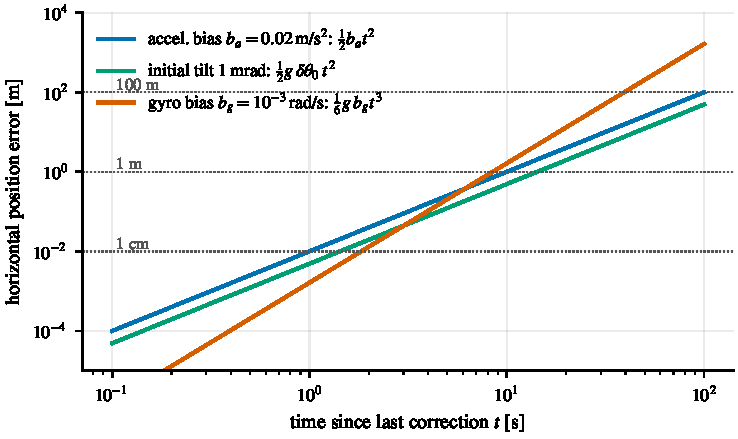
\includegraphics[width=0.86\textwidth]{fig_dr_drift.pdf}
  \caption{Deterministic dead-reckoning drift from three error sources of a consumer-grade IMU.
  A gyro bias of $10^{-3}$~rad/s ($\approx 0.06\,^\circ$/s) produces more than a meter of error
  after ten seconds and hundreds of meters after one minute. The cubic law is why attitude
  accuracy dominates inertial navigation.}
  \label{fig:dr-drift}
\end{figure}

With $b_g = 10^{-3}$~rad/s, a modest value for a MEMS gyroscope, the gyro term alone gives
$1.6$~m after 10~s and $353$~m after 60~s. Random sensor noise adds error that grows in a
similar way. \Cref{ch:errordyn} derives that the position \emph{standard deviation} due to
accelerometer white noise grows as $t^{3/2}$, due to gyroscope white noise as $t^{5/2}$, and due to
the gyroscope bias random walk as $t^{7/2}$.

\begin{keyidea}[inertial navigation is an attitude problem]
Because gravity is large (about $9.81~\mathrm{m/s^2}$) compared with typical accelerometer errors,
a tilt of one milliradian costs as much as an accelerometer bias of about
$10~\mathrm{mm/s^2}$. Position accuracy is therefore limited mostly by attitude accuracy. Any aiding
sensor that constrains roll and pitch, as a camera does, pays off enormously.
\end{keyidea}

\subsection{The camera}

A camera measures the \emph{directions} (bearings) of light rays arriving from the scene. A point
$p_f$ in the world appears in the image at the projection of its camera-frame coordinates
$p_c = (X_c, Y_c, Z_c)$:
\begin{equation}
  z = \begin{bmatrix} X_c/Z_c \\ Y_c/Z_c \end{bmatrix}.
\end{equation}
Because images are measurements of fixed scene geometry, they do not drift the way integrated
inertial data does. But a single camera has a fundamental blind spot.

\begin{proposition}[Monocular scale ambiguity]
\label{prop:scale-ambiguity}
Let a camera with poses $(R_i, p_i)$, $i = 1, \dots, M$, observe points $p_{f,j}$. For any $s > 0$, the
scaled configuration with poses $(R_i, s\,p_i)$ and points $s\,p_{f,j}$ produces exactly the same
images.
\end{proposition}
\begin{proof}
In camera $i$, the scaled point has coordinates
$R_i\T(s\,p_{f,j} - s\,p_i) = s\, R_i\T(p_{f,j} - p_i)$. The projection divides the first two
coordinates by the third, so the factor $s$ cancels.
\end{proof}

A camera alone therefore recovers the trajectory and the scene only up to an unknown global scale.
A photograph of a toy car from 10~cm can be identical to a photograph of a real car from 4~m. Cameras
also fail under motion blur, in darkness, against texture-less surfaces such as white walls, and in
scenes dominated by moving objects.

\subsection{Why the combination works}

\begin{table}[t]
\centering\small
\begin{tabularx}{\textwidth}{@{}>{\raggedright\arraybackslash}X >{\raggedright\arraybackslash}X >{\raggedright\arraybackslash}X@{}}
\toprule
 & \textbf{IMU} & \textbf{Monocular camera} \\
\midrule
Rate & 100--1000 Hz & 10--60 Hz \\
Measures & angular rate, specific force & bearings to scene points \\
Scale & metric & unknown (\cref{prop:scale-ambiguity}) \\
Drift & fast ($t^2$ to $t^3$) & slow, relative to the scene \\
Gravity direction & observable (at rest or on average) & not observable \\
Fails when & always drifts; saturates on impacts & blur, darkness, no texture, pure rotation \\
\bottomrule
\end{tabularx}
\caption{The IMU and the camera fail in complementary ways.}
\label{tab:sensor-complement}
\end{table}

\Cref{tab:sensor-complement} summarizes the complementarity. The camera bounds the inertial drift by
constraining the motion between images. The IMU supplies metric scale, the direction of gravity
(and hence absolute roll and pitch), high-rate motion between frames, and robustness during brief
visual outages. Scale becomes observable because the accelerometer measures acceleration in
$\mathrm{m/s^2}$: scaling a trajectory by $s$ scales its acceleration by $s$, which the
accelerometer would notice. The exception is unaccelerated motion. At constant velocity, the
scale is unobservable again, which is one of several \emph{degenerate motions} studied in
\cref{ch:observability}.

Even fused, four directions remain unobservable: the three components of global position, and the
rotation about the gravity vector (global yaw). Neither sensor senses where the origin is or which
way north is. VIO estimates these relative to the starting pose, and they drift.

\section{Why fusion is hard}

The difficulty of VIO comes from several sources acting at once.
\begin{enumerate}
  \item \textbf{Nonlinearity.} Rotations enter the equations through products and trigonometric
        functions, and the camera projection divides by depth.
  \item \textbf{Curved state spaces.} Orientations do not live in a vector space. You cannot add
        two rotations, and every estimator must deal with this (\cref{ch:lie}).
  \item \textbf{Multi-rate, asynchronous data.} The IMU runs at 200~Hz and the camera at 20~Hz,
        and every measurement must be processed in timestamp order.
  \item \textbf{Unknown scene.} The 3D positions of the visual features are unknown and must be
        estimated, or eliminated, along with the motion.
  \item \textbf{Outliers.} Feature tracks fail, latch onto moving objects, or slide along edges.
  \item \textbf{Unobservability.} Some directions of the state cannot be determined. A careless
        estimator can become falsely confident about them, which is the consistency problem of
        \cref{ch:observability}.
  \item \textbf{Real time.} All of this must run at camera rate, deterministically, on embedded
        processors.
\end{enumerate}

\section{A map of the field}

VIO algorithms differ along three main axes.

\paragraph{Loosely vs.\ tightly coupled.} A loosely coupled system runs a vision-only pipeline
that produces up-to-scale poses and fuses those poses with the IMU. A tightly coupled system feeds
the raw visual measurements (feature positions in the image) directly into a single estimator
together with the inertial data. Tight coupling is more accurate and more robust, because the IMU
helps the vision part and correlations are handled correctly. All modern high-accuracy systems,
and this project, are tightly coupled.

\paragraph{Filtering vs.\ optimization.} \emph{Filtering} approaches (EKF-based) process each
measurement once, keep a Gaussian belief over a bounded state, and discard the past. They are fast
and have predictable cost. \emph{Optimization} approaches solve a nonlinear least-squares problem
over a sliding window of recent states, relinearizing as needed, and summarize discarded states as
a prior (marginalization). They are typically more accurate per frame but more expensive and more
complex. The two families are closer than they appear: the MSCKF is equivalent to a single
Gauss--Newton iteration over a sliding window of poses with the landmarks marginalized
(\cref{ch:msckfupdate}).

\paragraph{Feature-based vs.\ direct.} Feature-based systems extract and track sparse keypoints and
use their image coordinates as measurements. Direct systems use pixel intensities themselves
(photometric error).

\begin{table}[t]
\centering\small
\begin{tabularx}{\textwidth}{@{}l l >{\raggedright\arraybackslash}X@{}}
\toprule
\textbf{System} & \textbf{Family} & \textbf{Notes} \\
\midrule
EKF-SLAM / MonoSLAM~\cite{davison2007monoslam} & filter, landmarks in state & cost grows quadratically with landmarks \\
MSCKF~\cite{mourikis2007msckf, li2013msckf2} & filter, poses in state & landmarks eliminated by nullspace projection; this project \\
MSCKF-VIO~\cite{sun2018msckfvio} & filter (stereo MSCKF) & open-source, fast flight; good engineering reference \\
OpenVINS~\cite{geneva2020openvins} & filter (MSCKF + SLAM features) & research platform with excellent documentation \\
ROVIO~\cite{bloesch2015rovio} & filter, direct & photometric patches in an iterated EKF \\
OKVIS~\cite{leutenegger2015okvis} & optimization, keyframes & sliding-window bundle adjustment \\
VINS-Mono~\cite{qin2018vins} & optimization & preintegration, robust initialization, loop closure \\
ORB-SLAM3~\cite{campos2021orbslam3} & optimization + map & full visual-inertial SLAM with relocalization \\
\bottomrule
\end{tabularx}
\caption{Representative visual-inertial estimators.}
\label{tab:vio-systems}
\end{table}

\section{Why the MSCKF}

In EKF-SLAM every tracked landmark adds three variables to the state. Covariance updates cost
$\mathcal{O}(n^2)$ to $\mathcal{O}(n^3)$ in the state size $n$, so a few hundred landmarks quickly
exhaust a real-time budget, and landmark initialization from a single camera is awkward because
depth is unknown at first sight.

The \textbf{Multi-State Constraint Kalman Filter} of Mourikis and Roumeliotis~\cite{mourikis2007msckf}
keeps instead a sliding window of past IMU poses, called \emph{clones}, taken at image times. When a
feature has been tracked across several clones, its observations constrain those poses relative to
one another. The feature's 3D position is triangulated temporarily, then algebraically
eliminated from the linearized equations by projecting onto the left nullspace of its Jacobian
(\cref{ch:msckfupdate}). The landmark never enters the state. The result:
\begin{itemize}
  \item cost linear in the number of features and bounded by the window size;
  \item no need to initialize landmark depth inside the filter;
  \item all the geometric information of each feature track is used exactly once.
\end{itemize}
These properties make the MSCKF the canonical filter-based VIO and an excellent vehicle for
learning, because it requires every ingredient of the field to be understood and nothing more.

\section{The estimator at a glance}

\begin{figure}[t]
\centering
\begin{tikzpicture}[node distance=7mm and 11mm]
  \node[block] (imu) {IMU\\ \footnotesize 200 Hz};
  \node[block, right=of imu] (prop) {Nominal propagation\\ \footnotesize Ch.~\ref{ch:strapdown}};
  \node[block, right=of prop] (cov) {Covariance propagation\\ \footnotesize Ch.~\ref{ch:errordyn}};
  \node[block, below=10mm of imu] (cam) {Camera\\ \footnotesize 20 Hz};
  \node[block, right=of cam] (front) {Front end: detect,\\ track, reject\\ \footnotesize Ch.~\ref{ch:frontend}};
  \node[block, right=of front] (clone) {Clone pose,\\ augment $P$\\ \footnotesize Ch.~\ref{ch:cloning}};
  \node[block, below=10mm of clone] (upd) {MSCKF update:\\ triangulate, project,\\ gate, update\\ \footnotesize Ch.~\ref{ch:msckfupdate}};
  \node[block, left=of upd] (inj) {Inject, reset,\\ marginalize\\ \footnotesize Ch.~\ref{ch:eskf}, \ref{ch:cloning}};
  \node[block, below=8mm of inj, fill=white] (out) {Pose, velocity,\\ biases, covariance};
  \coordinate (L) at ($(cam.west)+(-7mm,0)$);
  \coordinate (T) at ($(imu.north)+(0,6mm)$);
  \draw[->] (imu) -- (prop);
  \draw[->] (prop) -- (cov);
  \draw[->] (cam) -- (front);
  \draw[->] (front) -- node[note, above]{tracks} (clone);
  \draw[->] (cov) -- (clone);
  \draw[->] (clone) -- (upd);
  \draw[->] (upd) -- (inj);
  \draw[->] (inj) -- (out);
  \draw[->, dashed] (inj.west) -| (L) -- (L |- T) -| node[note, above, pos=0.25]{corrected state feeds back into propagation} (prop.north);
\end{tikzpicture}
\caption{Data flow of the monocular MSCKF built in these notes.}
\label{fig:pipeline}
\end{figure}

\Cref{fig:pipeline} shows the whole estimator. Between images, each IMU sample advances the nominal
state with the nonlinear kinematics and grows the error covariance. When an image arrives, the
filter propagates exactly to the image timestamp, appends a clone of the current pose, and updates
the feature tracks. Tracks that have ended, or whose oldest observation is about to leave the window,
are triangulated and converted into constraints between clones. The update corrects the IMU state and
all clones together, the correction is injected into the nominal state, and the oldest clone is
removed when the window is full. \Cref{ch:planar} builds a complete miniature of this pipeline for a robot moving in a plane,
small enough to derive by hand and to run as a short Python script; it is the place to look whenever the general chapters
feel abstract.

\begin{projectlink}[the road map]
The project builds this pipeline from the bottom up: the Lie group toolkit (M2), the data
stream (M3), inertial propagation (M4--M5), a filter tested against synthetic pose measurements
(M6--M7), the visual front end (M8--M9), and finally the MSCKF (M10a--M10b). Each layer is tested
in isolation before the next is added, so that any later failure can be localized.
\end{projectlink}

\section{The EuRoC benchmark}

The European Robotics Challenge (EuRoC) MAV dataset~\cite{burri2016euroc} is the standard VIO
benchmark. A hexacopter carries a stereo pair of global-shutter cameras ($752 \times 480$, 20~Hz)
and an ADIS16448 MEMS IMU (200~Hz), hardware-synchronized and calibrated. Eleven sequences fly
through an industrial machine hall (MH\_01 to MH\_05) and a motion-capture room (V1\_01 to V2\_03),
graded easy, medium and difficult by speed, lighting and texture. Ground truth comes from a laser
tracker or a motion-capture system. \Cref{app:euroc} documents the file formats and calibration
values the project uses.

\begin{takeaways}
\begin{itemize}
  \item VIO estimates pose, velocity and IMU biases from an IMU and a camera, with no map and no
        absolute positioning, and its error grows without bound.
  \item Inertial drift is dominated by attitude error: a gyro bias produces position error growing
        like $t^3$.
  \item A monocular camera observes the scene only up to scale. The accelerometer supplies the
        scale, provided the body accelerates.
  \item Global position and yaw remain unobservable even with both sensors.
  \item The MSCKF keeps a sliding window of past poses rather than landmarks, which bounds its cost
        while using every feature track.
\end{itemize}
\end{takeaways}

\begin{exercises}
  \item A MEMS accelerometer has a bias of $5~\mathrm{mg}$ ($1\,\mathrm{mg} = 9.81\times10^{-3}~\mathrm{m/s^2}$).
        How long can you dead-reckon before the position error exceeds 1~m? What gyro bias produces
        the same error at the same time?
  \item Prove that the gravity leak produced by a constant tilt error $\delta\theta_0$ is
        $g\,\delta\theta_0$ to first order. What is the exact expression, and at what tilt does the
        first-order formula err by 1\%?
  \item Extend \cref{prop:scale-ambiguity}: show that applying a common rigid transformation
        $(R, t)$ to all camera poses and points also leaves the images unchanged. How many
        unobservable degrees of freedom does a monocular camera have? Which of them does an IMU
        remove, and why?
  \item A drone hovers perfectly still for 30~s. Which states can a VIO system estimate during that
        time, and which cannot be distinguished from each other? (Revisit this after
        \cref{ch:observability}.)
  \item Read the abstract and introduction of~\cite{mourikis2007msckf}. In two sentences, state the
        problem with EKF-SLAM that the paper claims to solve, and the key idea of the solution.
\end{exercises}


\part{Mathematical Foundations}
\chapter{Linear Algebra for State Estimation}
\label{ch:linalg}

\begin{objectives}
\begin{itemize}
  \item Master the cross-product matrix $\sx{a}$ and the identities used in every Jacobian derivation.
  \item Understand the four fundamental subspaces, especially the \emph{left nullspace} on which the
        MSCKF rests.
  \item Know when and why to use Cholesky, LDL$^\mathsf{T}$, QR and SVD, and why a filter should never
        form an explicit inverse.
  \item Use block matrices, Schur complements and the Woodbury identity fluently.
  \item Understand the matrix exponential and floating-point arithmetic well enough to write
        numerically robust code.
\end{itemize}
\end{objectives}

Most of the computation in a Kalman filter is linear algebra: products of covariance matrices,
solutions of linear systems, and factorizations. This chapter collects the tools the rest of the
notes rely on and explains the numerical reasoning behind them. Readers fluent in numerical linear
algebra can skim it, but should not skip \cref{sec:skew,sec:subspaces,sec:floating}.

% ------------------------------------------------------------------------------
\section{Vectors, coordinates and the cross product}
\label{sec:skew}

\subsection{Vectors versus their coordinates}

A physical vector, such as a velocity or the direction of gravity, exists independently of any
coordinate system. To compute with it we express it in a \emph{frame}: an origin plus three
orthonormal, right-handed axes. The same physical vector $\vec{v}$ has different coordinate
triples $v_w \in \R^3$ and $v_b \in \R^3$ in the world and body frames, and the two are related by
a rotation matrix, $v_w = R_{wb}\,v_b$ (\cref{ch:rotations}). Confusing a vector with its
coordinates in some frame is the root of most frame bugs. Throughout these notes, a subscript on a
coordinate vector names the frame it is expressed in.

For coordinate vectors $a, b \in \R^3$ we use the standard inner product
$a\T b = \sum_i a_i b_i$, the Euclidean norm $\|a\| = \sqrt{a\T a}$, and the cross product
$a \times b$. The cross product is bilinear, anti-commutative ($a \times b = -b \times a$), and
orthogonal to both arguments. Its norm is $\|a\|\|b\|\sin\angle(a,b)$.

\subsection{The cross-product (skew-symmetric) matrix}

Because $a \times b$ is linear in $b$, it can be written as a matrix-vector product.

\begin{definition}[Skew-symmetric matrix]
For $a = (a_1, a_2, a_3)\T$, the \emph{cross-product matrix} of $a$ is
\begin{equation}
  \sx{a} = \begin{bmatrix} 0 & -a_3 & a_2 \\ a_3 & 0 & -a_1 \\ -a_2 & a_1 & 0 \end{bmatrix},
  \qquad\text{so that}\qquad \sx{a}\, b = a \times b \quad \forall\, b \in \R^3 .
  \label{eq:skew}
\end{equation}
It is skew-symmetric: $\sx{a}\T = -\sx{a}$. Conversely, every $3\times3$ skew-symmetric matrix
$S$ equals $\sx{s}$ for the unique vector $s = (S_{32}, S_{13}, S_{21})\T$. We write
$s = S\veeop$ for this inverse operation, the \emph{vee} map. In Lie theory, $\sx{\cdot}$ is
also written $(\cdot)\hatop$ and called the \emph{hat} map.
\end{definition}

The following identities are used constantly in derivations. Learn to recognize them on sight.

\begin{proposition}[Cross-product identities]
\label{prop:skew-identities}
For $a, b, c \in \R^3$ and $R \in \SO$ (a rotation matrix):
\begin{align}
  \sx{a}\, b &= -\sx{b}\, a, \label{eq:skew-anticomm}\\
  \sx{a}\, a &= 0, \label{eq:skew-self}\\
  \sx{a}^2 &= a a\T - \|a\|^2 I, \label{eq:skew-sq}\\
  \sx{a}^3 &= -\|a\|^2 \sx{a}, \label{eq:skew-cube}\\
  \sx{a}\sx{b} &= b a\T - (a\T b)\, I, \label{eq:skew-prod}\\
  \sx{a \times b} &= \sx{a}\sx{b} - \sx{b}\sx{a} = b a\T - a b\T, \label{eq:skew-commutator}\\
  \sx{R a} &= R \sx{a} R\T, \label{eq:skew-rot}\\
  R\,(a \times b) &= (Ra) \times (Rb). \label{eq:cross-rot}
\end{align}
\end{proposition}

\begin{proof}
\eqref{eq:skew-anticomm} and \eqref{eq:skew-self} restate $a\times b = -b\times a$ and
$a \times a = 0$. For \eqref{eq:skew-prod}, apply both sides to an arbitrary $c$ and use the
``BAC--CAB'' rule $a \times (b \times c) = b\,(a\T c) - c\,(a\T b)$:
$\sx{a}\sx{b}c = a\times(b\times c) = b a\T c - (a\T b) c$. Setting $b = a$ gives
\eqref{eq:skew-sq}, and multiplying \eqref{eq:skew-sq} by $\sx{a}$ and using \eqref{eq:skew-self}
gives \eqref{eq:skew-cube}. Subtracting \eqref{eq:skew-prod} from its version with $a, b$ swapped
gives the second equality of \eqref{eq:skew-commutator}. The first follows from the Jacobi identity
$a \times (b \times c) + b \times (c \times a) + c \times (a \times b) = 0$. For
\eqref{eq:cross-rot}, the cross product is defined by orientation and lengths, both preserved by a
proper rotation. Finally \eqref{eq:skew-rot} follows from \eqref{eq:cross-rot}:
$\sx{Ra}\, c = (Ra)\times c = (Ra)\times(R R\T c) = R\big(a \times R\T c\big) = R\sx{a}R\T c$.
\end{proof}

\begin{keyidea}[moving a vector out of a cross product]
Identity \eqref{eq:skew-anticomm} is how unknowns are isolated in Jacobian derivations. A
perturbation appears as $\sx{\delta\theta}\,v$, and the Jacobian with respect to $\delta\theta$ is
read off after rewriting it as $-\sx{v}\,\delta\theta$.
\end{keyidea}

Identity \eqref{eq:skew-cube} is what makes closed-form rotation formulas possible: every power of
$\sx{a}$ reduces to a multiple of $\sx{a}$ or $\sx{a}^2$, so infinite series in $\sx{a}$ collapse
to two terms (\cref{ch:rotations}).

% ------------------------------------------------------------------------------
\section{The four fundamental subspaces}
\label{sec:subspaces}

Let $A \in \R^{m\times n}$ have rank $r$. Four subspaces are associated with it:
\begin{center}
\begin{tabular}{@{}l l l l@{}}
\toprule
Subspace & Definition & Lives in & Dimension \\
\midrule
column space (range) & $\range(A) = \{Ax\}$ & $\R^m$ & $r$ \\
nullspace & $\nullsp(A) = \{x : Ax = 0\}$ & $\R^n$ & $n - r$ \\
row space & $\range(A\T)$ & $\R^n$ & $r$ \\
left nullspace & $\nullsp(A\T) = \{y : y\T A = 0\}$ & $\R^m$ & $m - r$ \\
\bottomrule
\end{tabular}
\end{center}

\begin{theorem}[Fundamental theorem of linear algebra]
\label{thm:fundamental}
$\nullsp(A) = \range(A\T)^\perp$ and $\nullsp(A\T) = \range(A)^\perp$. Consequently
$\R^n = \range(A\T) \oplus \nullsp(A)$ and $\R^m = \range(A) \oplus \nullsp(A\T)$, with
orthogonal direct sums.
\end{theorem}
\begin{proof}
$y \in \nullsp(A\T) \iff A\T y = 0 \iff x\T A\T y = 0\ \forall x \iff (Ax)\T y = 0\ \forall x
\iff y \perp \range(A)$. The first statement is the same argument applied to $A\T$.
\end{proof}

The \emph{left nullspace} deserves special attention because the MSCKF is built on it. Suppose a
stacked measurement depends on an unwanted variable $f$ through a tall matrix $H_f \in \R^{m\times
3}$ of full column rank:
\begin{equation}
  r = H_x\,\delta x + H_f\,\delta f + n .
\end{equation}
Take any matrix $A \in \R^{m\times(m-3)}$ whose columns form an orthonormal basis of
$\nullsp(H_f\T)$. Then $A\T H_f = 0$, and multiplying through by $A\T$ gives
$A\T r = A\T H_x\,\delta x + A\T n$: the unwanted variable has disappeared. \Cref{ch:msckfupdate}
shows that no information about $\delta x$ is lost in the process.

\begin{definition}[Orthogonal projector]
A matrix $\Pi$ is an orthogonal projector if $\Pi^2 = \Pi$ and $\Pi\T = \Pi$. If the columns of
$Q$ are an orthonormal basis of a subspace $\mathcal{S}$, the projector onto $\mathcal{S}$ is
$\Pi_{\mathcal{S}} = Q Q\T$. If $A$ has full column rank, the projector onto $\range(A)$ is
$A (A\T A)\inv A\T$, and $I - \Pi_{\mathcal{S}}$ projects onto $\mathcal{S}^\perp$.
\end{definition}

For the matrix $A$ spanning the left nullspace of $H_f$, these facts combine into an identity we
will use to prove the MSCKF's optimality:
\begin{equation}
  A A\T = I - H_f (H_f\T H_f)\inv H_f\T .
  \label{eq:nullspace-projector}
\end{equation}

% ------------------------------------------------------------------------------
\section{Symmetric and positive-definite matrices}

Covariance matrices are symmetric and positive semi-definite, and much of the numerical care in a
filter goes into keeping them that way.

\begin{definition}
A symmetric matrix $P = P\T \in \R^{n\times n}$ is \emph{positive semi-definite} (PSD, $P \succeq 0$) if
$x\T P x \ge 0$ for all $x$, and \emph{positive definite} (PD, $P \succ 0$) if $x\T P x > 0$
for all $x \ne 0$. We write $P_1 \succeq P_2$ (the Loewner order) if $P_1 - P_2 \succeq 0$.
\end{definition}

\begin{theorem}[Spectral theorem]
Every real symmetric matrix factors as $P = U \Lambda U\T$ with $U$ orthogonal and
$\Lambda = \diag(\lambda_1,\dots,\lambda_n)$ real. $P \succeq 0$ if and only if all
$\lambda_i \ge 0$, and $P \succ 0$ if and only if all $\lambda_i > 0$.
\end{theorem}

The geometric picture is an ellipsoid. For $P \succ 0$, the set $\{x : x\T P\inv x \le 1\}$ is an
ellipsoid with principal axes along the columns of $U$ and semi-axis lengths $\sqrt{\lambda_i}$.
This is the ``one-sigma'' uncertainty ellipsoid of a Gaussian with covariance $P$
(\cref{ch:prob}).

\begin{proposition}[Properties of PSD matrices]
\label{prop:psd}
Let $P, Q \succeq 0$ and let $A$ be any matrix of compatible size. Then
\begin{enumerate}
  \item $A P A\T \succeq 0$ (congruence preserves semi-definiteness);
  \item $P + Q \succeq 0$, and $P + Q \succ 0$ if either is PD;
  \item $P_{ii} \ge 0$ and $|P_{ij}| \le \sqrt{P_{ii} P_{jj}}$;
  \item every principal submatrix of $P$ is PSD.
\end{enumerate}
\end{proposition}
\begin{proof}
(1) $x\T A P A\T x = (A\T x)\T P (A\T x) \ge 0$. (2) is immediate. (3) and (4) follow from (1) with
$A$ a selection matrix, using the $2\times2$ determinant for the off-diagonal bound.
\end{proof}

Property (1) explains why the covariance updates $\Phi P \Phi\T + Q$ and the Joseph form
(\cref{ch:kf}) preserve semi-definiteness exactly in exact arithmetic: they are sums of congruences
of PSD matrices. The simpler update $(I - KH)P$ is \emph{not} a congruence, which is why it can lose
positive semi-definiteness under rounding.

% ------------------------------------------------------------------------------
\section{Matrix factorizations}

\subsection{Cholesky and LDL$^\mathsf{T}$}

\begin{theorem}[Cholesky factorization]
A symmetric matrix $S$ is positive definite if and only if $S = L L\T$ for a unique lower
triangular $L$ with positive diagonal.
\end{theorem}

The factor is computed column by column:
\begin{equation}
  L_{jj} = \Big( S_{jj} - \sum_{k<j} L_{jk}^2 \Big)^{1/2}, \qquad
  L_{ij} = \frac{1}{L_{jj}}\Big( S_{ij} - \sum_{k<j} L_{ik}L_{jk} \Big), \quad i > j,
\end{equation}
at a cost of about $n^3/3$ flops, half that of an LU factorization. The algorithm is backward
stable without pivoting, and it fails (a negative argument of the square root) exactly when $S$ is
not numerically positive definite. That makes it a useful diagnostic too. The variant
$S = L D L\T$ with unit-diagonal $L$ and diagonal $D$ avoids square roots, and with symmetric
pivoting (Eigen's \code{LDLT}) it also handles semi-definite matrices gracefully.

Cholesky factors \emph{whiten} correlated quantities. If $n \sim \N(0, S)$ and $S = LL\T$, then
$L\inv n \sim \N(0, I)$. This is how Mahalanobis distances are computed stably:
$r\T S\inv r = \|L\inv r\|^2$, with one triangular solve.

\subsection{QR factorization and Householder reflections}

\begin{definition}[Householder reflection]
For a nonzero $v \in \R^m$, the matrix $H_v = I - 2\, \dfrac{v v\T}{v\T v}$ reflects vectors across
the hyperplane orthogonal to $v$. It is symmetric and orthogonal, $H_v = H_v\T = H_v\inv$.
\end{definition}

Given any $x \in \R^m$, choosing $v = x + \operatorname{sign}(x_1)\|x\|\,e_1$ gives
$H_v x = -\operatorname{sign}(x_1)\|x\|\,e_1$: a single reflection zeroes every entry of $x$ below
the first. (The sign choice avoids cancellation when $x$ is already nearly parallel to $e_1$.)
Applying such reflections to the columns of $A \in \R^{m\times n}$, $m \ge n$, one after another
produces
\begin{equation}
  H_n \cdots H_2 H_1\, A = \begin{bmatrix} R_1 \\ 0 \end{bmatrix}
  \quad\Longleftrightarrow\quad
  A = Q \begin{bmatrix} R_1 \\ 0 \end{bmatrix} = \begin{bmatrix} Q_1 & Q_2 \end{bmatrix}
      \begin{bmatrix} R_1 \\ 0 \end{bmatrix} = Q_1 R_1,
  \label{eq:qr}
\end{equation}
with $Q = H_1 H_2\cdots H_n$ orthogonal, $R_1 \in \R^{n\times n}$ upper triangular, $Q_1 \in
\R^{m\times n}$ and $Q_2 \in \R^{m\times(m-n)}$. The cost is about $2mn^2 - \tfrac23 n^3$ flops.

\begin{proposition}[Nullspaces from QR]
\label{prop:qr-nullspace}
If $A$ has full column rank $n$ and $A = Q_1 R_1$ as in \eqref{eq:qr}, then the columns of $Q_1$
are an orthonormal basis of $\range(A)$ and the columns of $Q_2$ are an orthonormal basis of the
left nullspace $\nullsp(A\T)$. In particular $Q_2\T A = 0$.
\end{proposition}
\begin{proof}
$Q\T A = [R_1;\ 0]$, so $Q_2\T A = 0$. The columns of $Q_2$ are orthonormal and there are $m - n$ of
them, which is the dimension of $\nullsp(A\T)$.
\end{proof}

\begin{implnote}[never form $Q$]
$Q$ is $m\times m$ and dense, but it is defined by only $n$ reflection vectors. Libraries store
those vectors compactly in the lower triangle of the factored matrix. To compute $Q\T B$ for some
other matrix $B$, apply the $n$ reflections to $B$ one at a time, at a cost of $\mathcal{O}(mnk)$
for $B \in \R^{m\times k}$. Forming $Q$ explicitly would cost $\mathcal{O}(m^2 n)$ and $m^2$ storage.
In Eigen, \code{HouseholderQR::householderQ()} returns a lazy \code{HouseholderSequence} that can
be applied to $B$ without materializing $Q$. Whether a particular call allocates must be checked
with the allocation guard, not assumed.
\end{implnote}

A \emph{Givens rotation} zeroes a single entry by rotating two rows. It is the tool of choice when
the matrix is already nearly triangular or very sparse. The original MSCKF paper suggests Givens
rotations for its nullspace projection, because the feature Jacobian has a sparse block structure.

\subsection{The singular value decomposition}

\begin{theorem}[SVD]
Every $A \in \R^{m\times n}$ factors as $A = U \Sigma V\T$ with $U, V$ orthogonal and $\Sigma$
diagonal with entries $\sigma_1 \ge \sigma_2 \ge \dots \ge 0$, the \emph{singular values}.
\end{theorem}

The SVD reveals everything about $A$ at once. The rank is the number of nonzero singular values; the
first $r$ columns of $U$ and $V$ span the column and row spaces, and the remaining columns span the
left nullspace and the nullspace. The \emph{condition number} $\kappa(A) = \sigma_1/\sigma_n$
measures how much relative errors in the data can be amplified in the solution of a linear system.
The minimum-norm least-squares solution of $Ax \approx b$ is $x = A^+ b$ with the pseudo-inverse
$A^+ = V \Sigma^+ U\T$. The SVD is the most robust of the factorizations and also the most
expensive. In this project it appears in the linear triangulation of \cref{ch:multiview} and in
diagnostics.

% ------------------------------------------------------------------------------
\section{Solving linear systems and least squares}

\begin{pitfall}[explicit inverses]
Formulas such as $K = P H\T S\inv$ are notation, not algorithms. Computing $S\inv$ and then
multiplying costs about three times as much as solving, is less accurate, and destroys structure.
Factor $S$ once (Cholesky or LDL$^\mathsf{T}$) and solve: $S K\T = H P\T$ gives $K\T$ by two
triangular substitutions per column. Writing \code{S.ldlt().solve(Identity)} is still an explicit
inverse in disguise.
\end{pitfall}

\paragraph{Least squares.} Given an overdetermined system $Ax \approx b$ with $A \in \R^{m\times n}$
of full column rank, the least-squares solution minimizes $\|Ax - b\|^2$. Setting the gradient to zero
gives the \emph{normal equations} $A\T A x = A\T b$. They are cheap but square the condition number,
$\kappa(A\T A) = \kappa(A)^2$, which can lose half the significant digits. The QR approach is more
stable: with $A = Q_1R_1$, $\|Ax - b\|^2 = \|R_1 x - Q_1\T b\|^2 + \|Q_2\T b\|^2$, so
$x = R_1\inv Q_1\T b$ by back substitution, and the residual norm is $\|Q_2\T b\|$.

\paragraph{Weighted least squares.} If the errors have covariance $W$, minimize
$(Ax - b)\T W\inv (Ax - b)$. With $W = LL\T$ this is ordinary least squares on the whitened system
$L\inv A x \approx L\inv b$.

% ------------------------------------------------------------------------------
\section{Block matrices and the Schur complement}

Estimation constantly partitions vectors and matrices into blocks: IMU state versus clones, poses
versus landmarks. Block elimination is the basic tool.

\begin{proposition}[Block factorization and inverse]
\label{prop:block-inverse}
Let $M = \begin{bmatrix} A & B \\ C & D \end{bmatrix}$ with $A$ invertible, and define the
\emph{Schur complement} of $A$ in $M$, $M/A := D - C A\inv B$. Then
\begin{equation}
  M = \begin{bmatrix} I & 0 \\ C A\inv & I \end{bmatrix}
      \begin{bmatrix} A & 0 \\ 0 & M/A \end{bmatrix}
      \begin{bmatrix} I & A\inv B \\ 0 & I \end{bmatrix},
  \qquad \det M = \det A \cdot \det(M/A),
\end{equation}
and if $M/A$ is invertible,
\begin{equation}
  M\inv = \begin{bmatrix}
    A\inv + A\inv B\, (M/A)\inv\, C A\inv & -A\inv B\, (M/A)\inv \\
    -(M/A)\inv C A\inv & (M/A)\inv
  \end{bmatrix}.
\end{equation}
\end{proposition}
\begin{proof}
Multiply out the three factors. The inverse is the product of the inverses of the three factors in
reverse order, and the inverses of the unit-triangular block factors are obtained by negating their
off-diagonal blocks.
\end{proof}

For a symmetric $M$ with $A \succ 0$: $M \succ 0$ if and only if $M/A \succ 0$. The Schur
complement is the algebraic form of \emph{eliminating} a block of variables. \Cref{ch:prob} shows it
is exactly Gaussian marginalization in information form and conditioning in covariance form.

\begin{theorem}[Woodbury matrix identity]
\label{thm:woodbury}
For invertible $A$ and $C$ and conformable $U, V$,
\begin{equation}
  (A + U C V)\inv = A\inv - A\inv U \big( C\inv + V A\inv U \big)\inv V A\inv .
\end{equation}
\end{theorem}
\begin{proof}
Write the block matrix $\begin{bmatrix} A & U \\ V & -C\inv\end{bmatrix}$ and compute the
top-left block of its inverse in two ways with \cref{prop:block-inverse}: eliminating $A$ first gives
the right-hand side, and eliminating $-C\inv$ first gives $(A + UCV)\inv$.
\end{proof}

Woodbury connects the two forms of the Kalman update (\cref{ch:kf}). It says that a low-rank update
of a matrix gives a low-rank update of its inverse, which is why an update with $m$ measurements
needs only an $m\times m$ inverse no matter how large the state is.

% ------------------------------------------------------------------------------
\section{The matrix exponential}
\label{sec:matexp}

\begin{definition}
For $A \in \R^{n\times n}$, $\exp(A) = \sum_{k=0}^\infty \frac{A^k}{k!} = I + A + \tfrac12 A^2 + \tfrac16 A^3 + \cdots$.
The series converges absolutely for every $A$.
\end{definition}

\begin{proposition}[Properties of the matrix exponential]
\label{prop:matexp}
\begin{enumerate}
  \item $x(t) = \exp(tA)\, x_0$ is the unique solution of $\dot x = Ax$, $x(0) = x_0$.
  \item $\frac{\dd}{\dd t}\exp(tA) = A \exp(tA) = \exp(tA)\, A$.
  \item $\exp(A)\inv = \exp(-A)$, and $\det\exp(A) = e^{\tr A}$.
  \item $\exp(T A T\inv) = T \exp(A)\, T\inv$ for invertible $T$.
  \item If $AB = BA$ then $\exp(A + B) = \exp(A)\exp(B)$. \textbf{In general this fails.}
\end{enumerate}
\end{proposition}

The failure of property 5 for non-commuting matrices is the algebraic root of everything subtle
about rotations: two rotations generated by $\sx{a}$ and $\sx{b}$ do not compose into the rotation
generated by $\sx{a + b}$. \Cref{ch:lie} measures the discrepancy precisely.

\begin{example}[Nilpotent generator: the double integrator]
\label{ex:double-integrator}
For $F = \begin{bmatrix} 0 & 1 \\ 0 & 0 \end{bmatrix}$, $F^2 = 0$, so the series terminates:
$\exp(F\Dt) = \begin{bmatrix} 1 & \Dt \\ 0 & 1\end{bmatrix}$. This is the exact transition matrix of
position and velocity under zero acceleration. The inertial error dynamics of \cref{ch:errordyn}
have a similar nilpotent structure, so their exponentials can be written in closed form.
\end{example}

% ------------------------------------------------------------------------------
\section{Derivatives and Jacobians}

\begin{definition}[Jacobian layout]
For $f: \R^n \to \R^m$, the Jacobian $\frac{\partial f}{\partial x} \in \R^{m\times n}$ has
entries $\big[\frac{\partial f}{\partial x}\big]_{ij} = \frac{\partial f_i}{\partial x_j}$
(numerator layout), so that $f(x + \delta) = f(x) + \frac{\partial f}{\partial x}\delta +
o(\|\delta\|)$. Column $j$ is the sensitivity of the output to the $j$-th input direction. This
is exactly what a finite-difference test computes column by column.
\end{definition}

With this layout the chain rule reads
$\frac{\partial (g\circ f)}{\partial x} = \frac{\partial g}{\partial y}\big|_{y = f(x)}\frac{\partial f}{\partial x}$,
a product of matrices in the same order as the composition. A few derivatives recur:
\begin{equation}
  \frac{\partial (Ax)}{\partial x} = A, \qquad
  \frac{\partial (a \times x)}{\partial x} = \sx{a}, \qquad
  \frac{\partial (x \times a)}{\partial x} = -\sx{a}, \qquad
  \frac{\partial (x\T S x)}{\partial x} = x\T (S + S\T).
\end{equation}
\Cref{ch:lie} extends Jacobians to functions whose inputs or outputs are rotations.

% ------------------------------------------------------------------------------
\section{Floating-point arithmetic}
\label{sec:floating}

An IEEE~754 \code{double} stores a sign, an 11-bit exponent, and a 53-bit significand (52 stored
bits plus an implicit leading one). Two constants matter:
\begin{itemize}
  \item the \emph{machine epsilon} $\mach = 2^{-52} \approx 2.22\times10^{-16}$, the gap between $1$
        and the next larger double (\code{std::numeric\_limits<double>::epsilon()});
  \item the \emph{unit roundoff} $u = 2^{-53} \approx 1.11\times10^{-16}$: every basic operation
        satisfies $\mathrm{fl}(a \circ b) = (a\circ b)(1 + \delta)$ with $|\delta| \le u$.
\end{itemize}
Relative accuracy is therefore excellent for a single operation. Trouble comes from
\emph{cancellation}: subtracting two nearly equal numbers that each carry a rounding error leaves
a small result whose relative error can be enormous.

\begin{example}[Catastrophic cancellation in $1 - \cos\theta$]
\label{ex:cancellation}
For $\theta = 10^{-5}$, $\cos\theta = 1 - 5\times10^{-11} + \dots$. The stored value of
$\cos\theta$ has an absolute error up to $u \approx 10^{-16}$, so $1 - \cos\theta \approx
5\times 10^{-11}$ is computed with relative error up to $10^{-16}/(5\times10^{-11}) \approx 2\times
10^{-6}$. Dividing by $\theta^2$ to form $(1-\cos\theta)/\theta^2 \approx 1/2$ keeps that relative
error. At $\theta = 10^{-8}$, $\cos\theta$ rounds to exactly $1$, and the computed value is $0$
instead of $1/2$. The Taylor expansion $\tfrac12 - \tfrac{\theta^2}{24} + \cdots$ has no
cancellation at all. \Cref{fig:taylor} in \cref{ch:lie} shows this effect for all the coefficient
functions of the rotation group.
\end{example}

\begin{pitfall}[time stamps in floating point]
EuRoC timestamps are nanoseconds since the Unix epoch, about $1.4\times10^{18}$, which lies between
$2^{60}$ and $2^{61}$. A \code{double} near that value can only represent multiples of
$2^{60-52} = 256$~ns. Converting absolute timestamps to \code{double} therefore quantizes them to
256~ns, and accumulating time by repeated addition of $\Dt$ drifts further. Keep absolute time in
64-bit integers (\code{std::chrono::nanoseconds}) and convert only differences to \code{double}
(AGENTS.md C5).
\end{pitfall}

\paragraph{Finite-difference step size.} A finite-difference derivative is itself a cancellation.
For the central difference $\frac{f(x+h) - f(x-h)}{2h}$, the truncation error is about
$\frac{h^2}{6}|f'''|$ and the rounding error about $\frac{u |f|}{h}$. Their sum is minimized at
\begin{equation}
  h^\star = \left(\frac{3\,u\,|f|}{|f'''|}\right)^{1/3} \approx 10^{-5}\text{ to }10^{-6}
  \quad\text{(for quantities of order one)},
\end{equation}
with a total error of order $u^{2/3} \approx 10^{-11}$. For the one-sided difference the optimal step
is $\sim\sqrt{u} \approx 10^{-8}$ and the error is only $\sim 10^{-8}$. This is why Jacobian tests
use central differences with $h \approx 10^{-6}$ and tolerances around $10^{-6}$ to $10^{-8}$, scaled
to the magnitude of the quantities involved.

\paragraph{Conditioning versus stability.} A problem is \emph{ill-conditioned} if small changes in
its data produce large changes in its exact answer. An algorithm is \emph{unstable} if it produces
much larger errors than the conditioning of the problem justifies. Computing the rotation angle
from a rotation matrix with $\arccos$ near zero angle is an unstable algorithm for a
well-conditioned problem (\cref{ch:lie}). Triangulating a point seen with almost no parallax is an
ill-conditioned problem that no algorithm can rescue (\cref{ch:multiview}).

\begin{takeaways}
\begin{itemize}
  \item $\sx{a}b = a\times b = -\sx{b}a$, $\sx{a}^3 = -\|a\|^2\sx{a}$, and $\sx{Ra} = R\sx{a}R\T$ are
        the workhorses of every rotation derivation.
  \item The left nullspace of a tall matrix is the orthogonal complement of its column space.
        A full QR factorization delivers an orthonormal basis for it.
  \item Covariance updates should be congruences ($APA\T$) plus PSD terms, so that positive
        semi-definiteness is preserved structurally.
  \item Factor and solve; never form an explicit inverse, and never form $Q$ explicitly.
  \item Schur complements eliminate variables; Woodbury converts between large and small inverses.
  \item Cancellation, not single operations, destroys floating-point accuracy. Time stamps belong
        in 64-bit integers.
\end{itemize}
\end{takeaways}

\begin{exercises}
  \item Prove \eqref{eq:skew-commutator} directly from \eqref{eq:skew-prod}, and verify the Jacobi
        identity numerically for random vectors.
  \item Show that the eigenvalues of $\sx{a}$ are $0$ and $\pm i\|a\|$. Which eigenvector belongs to $0$?
  \item Let $H_f \in \R^{2M\times3}$ have full column rank. Compute the dimension of its left
        nullspace for $M = 2, 3, 10$. Prove \eqref{eq:nullspace-projector}.
  \item Show that if $P\succ0$ then $P - K S K\T \succeq 0$ for $S = HPH\T + R$, $K = PH\T S\inv$
        and $R \succ 0$. (Hint: Schur complement of a suitable $2\times2$ block matrix.)
  \item Implement Householder QR in Python for a $10\times3$ matrix and check
        \cref{prop:qr-nullspace} numerically. Then compare the accuracy of solving a least-squares
        problem with $\kappa(A) = 10^8$ by the normal equations and by QR.
  \item Use \cref{thm:woodbury} to show that
        $\big(P\inv + H\T R\inv H\big)\inv = P - PH\T(HPH\T + R)\inv HP$. Which side is cheaper to
        evaluate when $P$ is $75\times75$ and $R$ is $2\times2$? When $R$ is $500\times500$?
  \item What is the spacing of doubles near $2^{30}$ seconds expressed in nanoseconds? Would storing
        time as \code{double} seconds since the epoch be acceptable for a 200~Hz IMU?
  \item For $f(x) = \sin x$ at $x = 1$, plot the error of forward and central differences versus
        $h \in [10^{-16}, 10^{-1}]$ on log axes and locate the optimal step sizes. Compare with the
        formulas above.
\end{exercises}

\chapter{Numerical Linear Algebra}
\label{ch:numlinalg}

\begin{objectives}
\begin{itemize}
  \item Count the cost of matrix operations and understand why a filter must never form an explicit inverse.
  \item Derive the LU, Cholesky, QR and singular value decompositions, and know which one to use when.
  \item Solve least-squares problems stably, and compute nullspaces, projectors and pseudo-inverses.
  \item Use block matrices, Schur complements and the Woodbury identity fluently.
  \item Understand the matrix exponential, and why the exponential of a skew-symmetric matrix is a rotation.
  \item Understand floating-point arithmetic: rounding, cancellation, conditioning and stability.
\end{itemize}
\end{objectives}

\Cref{ch:linalg} described what matrices \emph{are}. This chapter is about computing with them reliably. A Kalman filter
spends nearly all of its time in a few operations: multiplying matrices, solving linear systems with a covariance matrix,
and factorizing Jacobians. Done naively, these operations are slow, lose accuracy, or silently destroy the symmetry and
positive definiteness of covariances. Done well, they are fast and accurate to nearly machine precision.

% ==============================================================================
\section{The cost of matrix operations}

Numerical analysts count \term{flops} (floating-point operations: one addition or multiplication each). Some basic costs
for $n\times n$ matrices:
\begin{center}\small
\begin{tabular}{@{}l l@{}}
\toprule
Operation & Approximate flops \\
\midrule
dot product of two $n$-vectors & $2n$ \\
matrix-vector product & $2n^2$ \\
matrix-matrix product & $2n^3$ \\
solving a triangular system & $n^2$ \\
LU factorization & $\tfrac23n^3$ \\
Cholesky factorization & $\tfrac13n^3$ \\
explicit inverse & $2n^3$ \\
\bottomrule
\end{tabular}
\end{center}
For the MSCKF with $n = 75$, a matrix product costs about $8\times10^5$ flops, a fraction of a millisecond. Costs grow with the cube of
the dimension, which is why filters keep their state small, exploit block structure, and update only the blocks that change.
We write $\mathcal{O}(n^3)$ (``order $n^3$'') to mean ``at most a constant times $n^3$ for large $n$''.

% ==============================================================================
\section{Triangular systems and the LU factorization}

\subsection{Forward and back substitution}

A triangular system is solved by direct substitution. For an upper-triangular $U$ with non-zero diagonal, the last equation
$U_{nn}x_n = b_n$ gives $x_n$, the previous one then gives $x_{n-1}$, and so on:
\begin{equation}
  x_i = \frac{1}{U_{ii}}\Big(b_i - \sum_{j>i}U_{ij}x_j\Big), \qquad i = n, n-1, \dots, 1 .
\end{equation}
This is \term{back substitution}; \emph{forward substitution} solves lower-triangular systems from the top. Each costs about $n^2$
flops. Every method in this chapter reduces a hard problem to one or two triangular solves.

\subsection{LU factorization}

Gaussian elimination (\cref{sec:linsys}) subtracts multiples $\ell_{ik}$ of row $k$ from the rows below it, column by column, until
the matrix is upper triangular. Recording the multipliers in a unit lower-triangular matrix $L$ gives the \term{LU factorization}
\begin{equation}
  A = LU .
\end{equation}
Then $Ax = b$ is solved by forward substitution $Ly = b$ and back substitution $Ux = y$. The factorization costs $\tfrac23n^3$ flops
once; every additional right-hand side costs only $2n^2$.

\paragraph{Pivoting.} Elimination divides by the pivots. A tiny pivot creates huge multipliers that amplify rounding errors.
The classic example is $\begin{bmatrix}10^{-20} & 1\\ 1 & 1\end{bmatrix}$: eliminating with the pivot $10^{-20}$ gives a multiplier
of $10^{20}$, and in double precision the computed solution of $Ax = (1, 2)$ is completely wrong, although the matrix is
perfectly well conditioned. Swapping the two rows first fixes it. \emph{Partial pivoting} always swaps the row with the largest
available pivot into place, giving $PA = LU$ with a permutation matrix $P$. Symmetric positive-definite matrices, which is
what filters mostly factor, need no pivoting at all, as the next section shows.

% ==============================================================================
\section{The Cholesky factorization}

\begin{theorem}[Cholesky factorization]
\label{thm:cholesky}
\index{Cholesky factorization}
A symmetric matrix $S$ is positive definite if and only if $S = LL\T$ for a lower-triangular $L$ with positive diagonal.
This $L$ is unique.
\end{theorem}
\begin{proof}
If $S = LL\T$ with $L$ invertible, then $x\T Sx = \|L\T x\|^2 > 0$ for $x \ne 0$. Conversely, partition
\begin{equation*}
  S = \begin{bmatrix} s_{11} & s\T \\ s & S_{22} \end{bmatrix}
    = \begin{bmatrix} \ell_{11} & 0 \\ \ell & L_{22} \end{bmatrix}\begin{bmatrix} \ell_{11} & \ell\T \\ 0 & L_{22}\T \end{bmatrix}
    = \begin{bmatrix} \ell_{11}^2 & \ell_{11}\ell\T \\ \ell_{11}\ell & \ell\ell\T + L_{22}L_{22}\T \end{bmatrix}.
\end{equation*}
Matching blocks: $\ell_{11} = \sqrt{s_{11}}$ (positive because $s_{11} = e_1\T Se_1 > 0$), $\ell = s/\ell_{11}$, and
$L_{22}L_{22}\T = S_{22} - ss\T/s_{11}$. The last matrix (a Schur complement, \cref{sec:schur}) is again positive definite, so the
construction continues recursively on a matrix one size smaller. Each step is forced, which proves uniqueness.
\end{proof}

Unrolling the recursion column by column gives the algorithm
\begin{equation}
  L_{jj} = \Big( S_{jj} - \sum_{k<j} L_{jk}^2 \Big)^{1/2}, \qquad
  L_{ij} = \frac{1}{L_{jj}}\Big( S_{ij} - \sum_{k<j} L_{ik}L_{jk} \Big), \quad i > j,
\end{equation}
at a cost of $\tfrac13n^3$ flops, half that of LU. The algorithm is backward stable without pivoting, and it fails (the argument
of a square root is not positive) exactly when $S$ is not numerically positive definite, which makes it a useful diagnostic
too. The variant $S = LDL\T$, with unit-diagonal $L$ and diagonal $D$, avoids square roots; with symmetric pivoting (Eigen's
\code{LDLT}) it also handles semi-definite and slightly indefinite matrices gracefully.

\paragraph{Uses of the Cholesky factor.}
\begin{itemize}
  \item \emph{Solving} $Sx = b$: forward-substitute $Ly = b$, back-substitute $L\T x = y$.
  \item \emph{Whitening}: if a random vector $n$ has covariance $S = LL\T$, then $L\inv n$ has covariance $I$ (\cref{ch:prob}).
        Mahalanobis distances are computed as $r\T S\inv r = \|L\inv r\|^2$ with a single triangular solve.
  \item \emph{Sampling}: if $s$ has covariance $I$, then $Ls$ has covariance $S$.
  \item \emph{Determinants}: $\det S = \prod_iL_{ii}^2$, and $\log\det S = 2\sum_i\log L_{ii}$ without overflow.
\end{itemize}

% ==============================================================================
\section{Orthogonal factorizations: QR}

Orthogonal transformations do not amplify errors (they preserve lengths), so factorizations built from them are the most
stable available.

\subsection{QR from Gram--Schmidt}

Applying Gram--Schmidt to the columns $a_1, \dots, a_n$ of a full-column-rank $A \in \R^{m\times n}$ produces orthonormal $q_1, \dots, q_n$
with $a_k = \sum_{j\le k}r_{jk}q_j$, where $r_{jk} = q_j\T a_k$ and $r_{kk} = \|\tilde q_k\|$. In matrix form
\begin{equation}
  A = Q_1R_1, \qquad Q_1 = [q_1 \cdots q_n] \in \R^{m\times n},\quad Q_1\T Q_1 = I,\quad R_1 \text{ upper triangular}.
\end{equation}
This is the \term{QR factorization}. Classical Gram--Schmidt, implemented literally, loses orthogonality in floating point when the
columns are nearly dependent; the computed $q$'s drift away from being orthogonal. Householder reflections avoid this problem.

\subsection{Householder reflections}

\begin{definition}[Householder reflection]
\index{Householder reflection}
For a non-zero $v \in \R^m$, the matrix $H_v = I - 2\, \dfrac{v v\T}{v\T v}$ reflects vectors across the hyperplane orthogonal to $v$:
it reverses the component along $v$ and leaves the orthogonal components unchanged. It is symmetric and orthogonal, and is its own
inverse: $H_v = H_v\T = H_v\inv$.
\end{definition}

\begin{proposition}[Zeroing a vector below its first entry]
For $x \in \R^m$ not a multiple of $e_1$, let $\alpha = -\operatorname{sign}(x_1)\|x\|$ and $v = x - \alpha e_1$. Then $H_vx = \alpha e_1$.
\end{proposition}
\begin{proof}
Because $\|x\| = \|\alpha e_1\|$, the vectors $x$ and $\alpha e_1$ have the same length, so the reflection across the
perpendicular bisector of the segment joining them swaps them. That bisecting hyperplane is orthogonal to $v = x - \alpha e_1$.
Algebraically: $v\T v = 2\|x\|^2 - 2\alpha x_1$ and $v\T x = \|x\|^2 - \alpha x_1 = \tfrac12v\T v$, so
$H_vx = x - 2v\,\frac{v\T x}{v\T v} = x - v = \alpha e_1$.
\end{proof}

The sign choice makes $v_1 = x_1 + \operatorname{sign}(x_1)\|x\|$ a sum of two numbers of the same sign, avoiding the cancellation
that the other choice would suffer when $x$ is nearly parallel to $e_1$.

\paragraph{Householder QR.} Apply a reflection $H_1$ that zeroes the first column of $A$ below the diagonal; then a reflection $H_2$,
acting on rows $2, \dots, m$, that zeroes the second column below the diagonal; and so on for all $n$ columns:
\begin{equation}
  H_n \cdots H_2 H_1\, A = \begin{bmatrix} R_1 \\ 0 \end{bmatrix}
  \quad\Longleftrightarrow\quad
  A = Q \begin{bmatrix} R_1 \\ 0 \end{bmatrix} = \begin{bmatrix} Q_1 & Q_2 \end{bmatrix}
      \begin{bmatrix} R_1 \\ 0 \end{bmatrix} = Q_1 R_1,
  \label{eq:qr}
\end{equation}
with $Q = H_1 H_2\cdots H_n$ orthogonal ($m\times m$), $R_1 \in \R^{n\times n}$ upper triangular, $Q_1 \in \R^{m\times n}$ and $Q_2 \in \R^{m\times(m-n)}$. The
cost is about $2mn^2 - \tfrac23 n^3$ flops. The form $A = Q[R_1; 0]$ is the \emph{full} QR factorization, and $A = Q_1R_1$ the
\emph{thin} one.

\paragraph{Applying $Q\T$ without forming $Q$.} Each $H_k$ is determined by its vector $v_k$, so $Q\T b = H_n\cdots H_1b$ is computed by
applying the reflections one at a time:
\begin{equation}
  b \;\gets\; b - v_k\,\frac{2\,v_k\T b}{v_k\T v_k}, \qquad k = 1, \dots, n,
\end{equation}
at a cost of $\mathcal{O}(m)$ per reflection. Forming $Q$ explicitly would cost $\mathcal{O}(m^2n)$ flops and $m^2$ storage.

\begin{proposition}[Nullspaces from QR]
\label{prop:qr-nullspace}
If $A$ has full column rank $n$ and $A = Q_1 R_1$ as in \eqref{eq:qr}, then the columns of $Q_1$ are an orthonormal basis of
$\range(A)$ and the columns of $Q_2$ are an orthonormal basis of the left nullspace $\nullsp(A\T)$. In particular $Q_2\T A = 0$.
\end{proposition}
\begin{proof}
$Q\T A = [R_1;\ 0]$, so $Q_2\T A = 0$, i.e.\ the columns of $Q_2$ lie in $\nullsp(A\T)$. They are orthonormal and there are $m - n$ of them,
which is the dimension of $\nullsp(A\T)$ by rank--nullity. Since $R_1$ is invertible, $\range(A) = \range(Q_1)$.
\end{proof}

\begin{implnote}[never form $Q$]
Libraries store the Householder vectors compactly in the lower triangle of the factored matrix. In Eigen,
\code{HouseholderQR::householderQ()} returns a lazy \code{HouseholderSequence} that can be applied to another matrix without
materializing $Q$. This is exactly what the MSCKF needs: it applies the reflections that triangularize a feature Jacobian to the
rest of the measurement equations (\cref{ch:msckfupdate}). Whether a particular call allocates must be checked with the allocation
guard, not assumed.
\end{implnote}

\subsection{Givens rotations}

A \term{Givens rotation} zeroes one entry at a time by rotating a pair of rows. To zero $b$ in the pair $(a, b)$, set
$r = \sqrt{a^2 + b^2}$, $c = a/r$ and $s = b/r$:
\begin{equation}
  \begin{bmatrix} c & s \\ -s & c \end{bmatrix}\begin{bmatrix} a \\ b \end{bmatrix} = \begin{bmatrix} r \\ 0 \end{bmatrix}.
\end{equation}
Embedded in an identity matrix, it acts on two rows of a larger matrix and leaves the others untouched. Givens rotations are
preferred when only a few entries need to be zeroed, when the matrix is sparse, or when rows arrive one at a time. The original
MSCKF paper suggests them for its nullspace projection, because the feature Jacobian has a sparse block structure.

% ==============================================================================
\section{Least squares}
\label{sec:least-squares}

\subsection{The problem and the normal equations}

An overdetermined system $Ax \approx b$, with $A \in \R^{m\times n}$, $m > n$, generally has no exact solution. The \term{least-squares}
solution minimizes the squared residual
\begin{equation}
  f(x) = \|Ax - b\|^2 = x\T A\T Ax - 2x\T A\T b + b\T b .
\end{equation}
Setting the gradient $2A\T Ax - 2A\T b$ to zero gives the \term{normal equations}
\begin{equation}
  A\T A\,x = A\T b .
  \label{eq:normal-equations}
\end{equation}
If $A$ has full column rank, $A\T A$ is positive definite (since $x\T A\T Ax = \|Ax\|^2 > 0$ for $x\ne0$), so the solution is unique and is
a minimum.

\paragraph{Geometric meaning.} The normal equations say $A\T(b - Ax) = 0$: the residual is orthogonal to every column of $A$. The fitted
vector $Ax$ is the orthogonal projection of $b$ onto $\range(A)$, the closest point to $b$ that the model can produce.

\begin{definition}[Orthogonal projector]
\index{projector}
A matrix $\Pi$ is an orthogonal projector if $\Pi^2 = \Pi$ and $\Pi\T = \Pi$. If the columns of $Q$ are an orthonormal basis of a subspace
$\mathcal{S}$, the projector onto $\mathcal{S}$ is $\Pi_{\mathcal{S}} = QQ\T$. For $A$ of full column rank the projector onto $\range(A)$ is
$A(A\T A)\inv A\T$, and $I - \Pi$ projects onto the orthogonal complement.
\end{definition}

Combining the two descriptions of the projector onto $\range(A)$, and recalling that the columns of $Q_2$ in \eqref{eq:qr} span its
complement $\nullsp(A\T)$, gives an identity we will use to prove the optimality of the MSCKF: for any $A_\perp$ whose columns are an
orthonormal basis of the left nullspace of a full-column-rank $H_f$,
\begin{equation}
  A_\perp A_\perp\T = I - H_f (H_f\T H_f)\inv H_f\T .
  \label{eq:nullspace-projector}
\end{equation}

\subsection{Three ways to solve}

\paragraph{Cholesky on the normal equations.} Form $A\T A$ ($mn^2$ flops) and factor it. This is the fastest method, but forming
$A\T A$ squares the condition number of the problem (\cref{sec:conditioning}): $\kappa(A\T A) = \kappa(A)^2$. When $\kappa(A) = 10^8$,
the normal equations lose essentially all sixteen significant digits.

\paragraph{QR.} With $A = Q[R_1; 0]$ and the invariance of lengths under $Q\T$,
\begin{equation}
  \|Ax - b\|^2 = \|Q\T(Ax - b)\|^2 = \|R_1x - Q_1\T b\|^2 + \|Q_2\T b\|^2 .
\end{equation}
The second term does not depend on $x$, and the first vanishes for $x = R_1\inv Q_1\T b$, computed by back substitution. The minimum
residual is $\|Q_2\T b\|$. This method works with the condition number of $A$ itself and is the standard choice.

\paragraph{SVD.} The most robust and most expensive method, required when $A$ may be rank deficient (\cref{sec:svd}).

\subsection{Weighted least squares}

When the equations have different reliabilities, with errors of covariance $W$, the right objective weights each residual by its
uncertainty (\cref{ch:estimation}):
\begin{equation}
  \min_x\ (Ax - b)\T W\inv(Ax - b) .
\end{equation}
With $W = LL\T$ this is ordinary least squares on the \emph{whitened} system $L\inv Ax \approx L\inv b$, and the normal equations become
$A\T W\inv A\,x = A\T W\inv b$.

% ==============================================================================
\section{The singular value decomposition}
\label{sec:svd}

\begin{theorem}[Singular value decomposition]
\label{thm:svd}
\index{singular value decomposition}
Every $A \in \R^{m\times n}$ can be written as $A = U\Sigma V\T$ with $U \in \R^{m\times m}$ and $V \in \R^{n\times n}$ orthogonal and
$\Sigma \in \R^{m\times n}$ diagonal with entries $\sigma_1 \ge \sigma_2 \ge \dots \ge 0$, the \term{singular values}.
\end{theorem}
\begin{proof}[Construction]
$A\T A$ is symmetric and PSD, so by the spectral theorem $A\T A = V\Lambda V\T$ with orthonormal $v_i$ and eigenvalues
$\lambda_1 \ge \dots \ge \lambda_n \ge 0$. Set $\sigma_i = \sqrt{\lambda_i}$. For each $\sigma_i > 0$ define $u_i = Av_i/\sigma_i$. These are
orthonormal: $u_i\T u_j = v_i\T A\T Av_j/(\sigma_i\sigma_j) = \lambda_jv_i\T v_j/(\sigma_i\sigma_j) = \delta_{ij}$. Complete them to an
orthonormal basis $u_1, \dots, u_m$ of $\R^m$. Then $Av_i = \sigma_iu_i$ for all $i$ (for $\sigma_i = 0$, $\|Av_i\|^2 = \lambda_i = 0$),
which in matrix form is $AV = U\Sigma$.
\end{proof}

\begin{figure}[t]
  \centering
  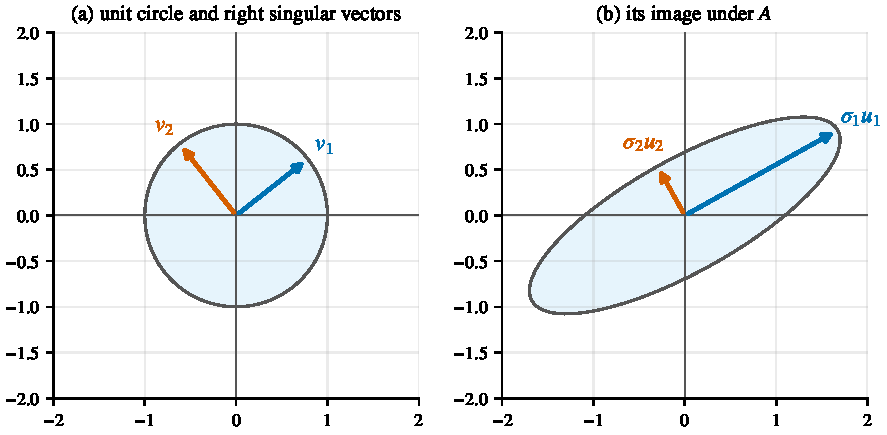
\includegraphics[width=0.9\textwidth]{fig_svd_geometry.pdf}
  \caption{Geometry of the SVD of a $2\times2$ matrix. The right singular vectors $v_1, v_2$ (left) form an orthonormal basis that $A$ maps
  to orthogonal vectors $\sigma_1u_1, \sigma_2u_2$ (right). The unit circle becomes an ellipse with semi-axes $\sigma_1$ and $\sigma_2$: every
  linear map is a rotation, an axis-aligned scaling, and another rotation.}
  \label{fig:svd}
\end{figure}

The SVD says that every linear map, in suitable orthonormal bases of its domain and codomain, is a pure scaling (\cref{fig:svd}). It
reveals everything about $A$ at once:
\begin{itemize}
  \item the rank $r$ is the number of non-zero singular values;
  \item $u_1, \dots, u_r$ span $\range(A)$, $u_{r+1}, \dots, u_m$ span $\nullsp(A\T)$, $v_1, \dots, v_r$ span $\range(A\T)$ and
        $v_{r+1}, \dots, v_n$ span $\nullsp(A)$;
  \item $\|A\|_2 = \sigma_1$ and $\|A\|_F^2 = \sum_i\sigma_i^2$.
\end{itemize}

\paragraph{Pseudo-inverse.} The \term{pseudo-inverse} $A^+ = V\Sigma^+U\T$, where $\Sigma^+$ inverts the non-zero singular values and transposes
the shape, gives the minimum-norm least-squares solution $x = A^+b$ of any system, including rank-deficient ones. For full column
rank, $A^+ = (A\T A)\inv A\T$.

\begin{proposition}[Homogeneous least squares]
\label{prop:homogeneous-ls}
\index{homogeneous least squares}
The unit vector $x$ minimizing $\|Ax\|$ is the right singular vector $v_n$ belonging to the smallest singular value, and the minimum is
$\sigma_n$.
\end{proposition}
\begin{proof}
$\|Ax\|^2 = x\T A\T Ax$, and by the Rayleigh quotient (\cref{prop:rayleigh}) its minimum over unit vectors is the smallest eigenvalue of
$A\T A$, $\sigma_n^2$, attained at the corresponding eigenvector $v_n$.
\end{proof}

Many geometric estimation problems have the form $Ax = 0$ with $x$ known only up to scale: estimating an essential matrix or a homography
from correspondences, or triangulating a point in homogeneous coordinates (\cref{ch:multiview}). With noisy data there is no exact
solution, and \cref{prop:homogeneous-ls} gives the best one.

\begin{theorem}[Best low-rank approximation, Eckart--Young]
\index{Eckart--Young theorem}
Among all matrices of rank at most $k$, the one closest to $A$ in the Frobenius or 2-norm is $A_k = \sum_{i\le k}\sigma_iu_iv_i\T$, obtained by
zeroing all but the $k$ largest singular values.
\end{theorem}

This is how an estimated matrix is projected onto a set defined by its singular values: for example, the nearest valid essential matrix to a
noisy estimate is obtained by replacing its singular values by $(1, 1, 0)$ (\cref{ch:multiview}).

% ==============================================================================
\section{Conditioning and stability}
\label{sec:conditioning}

Two different things can make a computed answer inaccurate: the problem itself may be sensitive to its data, or the algorithm may add more
error than necessary.

\begin{definition}[Condition number]
\index{condition number}
For an invertible (or full-column-rank) $A$, $\kappa(A) = \sigma_{\max}/\sigma_{\min} = \|A\|_2\,\|A^+\|_2$.
\end{definition}

\begin{proposition}[Sensitivity of linear systems]
If $Ax = b$ and $A(x + \delta x) = b + \delta b$, then $\dfrac{\|\delta x\|}{\|x\|} \le \kappa(A)\,\dfrac{\|\delta b\|}{\|b\|}$.
\end{proposition}
\begin{proof}
$\delta x = A\inv\delta b$ gives $\|\delta x\| \le \|A\inv\|\|\delta b\|$, and $b = Ax$ gives $\|b\| \le \|A\|\|x\|$. Multiply the two
inequalities.
\end{proof}

A problem with condition number $\kappa$ can lose about $\log_{10}\kappa$ significant digits whatever the algorithm; it is
\emph{ill-conditioned} when $\kappa$ is large. An algorithm is \emph{backward stable} if its computed answer is the exact answer to a
problem whose data differ from the true data by a few units of rounding error; such an algorithm never loses more than the
conditioning dictates. Householder QR, Cholesky on positive-definite matrices and LU with partial pivoting are backward stable in
practice; classical Gram--Schmidt and the normal equations for ill-conditioned least squares are not. In geometric terms:
triangulating a point seen with almost no parallax is an ill-conditioned problem that no algorithm can rescue
(\cref{ch:multiview}), while recovering the rotation angle from a rotation matrix with $\arccos$ is an unstable algorithm for a
well-conditioned problem (\cref{ch:lie}).

\begin{pitfall}[explicit inverses]
Formulas such as $K = P H\T S\inv$ are notation, not algorithms. Computing $S\inv$ and then multiplying costs about three times as much as
solving, is less accurate, and destroys structure. Factor $S$ once (Cholesky or LDL$^\mathsf{T}$) and solve: $S K\T = H P\T$ gives $K\T$
by two triangular substitutions per column. Writing \code{S.ldlt().solve(Identity)} is still an explicit inverse in disguise.
\end{pitfall}

% ==============================================================================
\section{Block matrices and the Schur complement}
\label{sec:schur}

Estimation constantly partitions vectors and matrices into blocks: IMU state versus clones, poses versus landmarks. Block elimination is
the basic tool.

\begin{proposition}[Block factorization and inverse]
\label{prop:block-inverse}
\index{Schur complement}
Let $M = \begin{bmatrix} A & B \\ C & D \end{bmatrix}$ with $A$ invertible, and define the \term{Schur complement} of $A$ in $M$,
$M/A := D - C A\inv B$. Then
\begin{equation}
  M = \begin{bmatrix} I & 0 \\ C A\inv & I \end{bmatrix}
      \begin{bmatrix} A & 0 \\ 0 & M/A \end{bmatrix}
      \begin{bmatrix} I & A\inv B \\ 0 & I \end{bmatrix},
  \qquad \det M = \det A \cdot \det(M/A),
\end{equation}
and if $M/A$ is invertible,
\begin{equation}
  M\inv = \begin{bmatrix}
    A\inv + A\inv B\, (M/A)\inv\, C A\inv & -A\inv B\, (M/A)\inv \\
    -(M/A)\inv C A\inv & (M/A)\inv
  \end{bmatrix}.
\end{equation}
\end{proposition}
\begin{proof}
Multiply out the three factors. The inverse is the product of the inverses of the three factors in reverse order, and the inverse of a
unit block-triangular factor is obtained by negating its off-diagonal block.
\end{proof}

The Schur complement is what remains of the equations for the second block of unknowns after the first block has been eliminated. To see
this, solve $\begin{bmatrix}A & B\\C & D\end{bmatrix}\begin{bmatrix}x\\y\end{bmatrix} = \begin{bmatrix}f\\g\end{bmatrix}$ by eliminating
$x = A\inv(f - By)$ from the second equation: $(D - CA\inv B)\,y = g - CA\inv f$. For symmetric $M$ with $A \succ 0$, $M \succ 0$ if and only if
$M/A \succ 0$. \Cref{ch:prob} shows that the Schur complement is exactly Gaussian conditioning in covariance form and marginalization in
information form, and \cref{ch:nlls} uses it to eliminate landmarks from bundle adjustment.

\begin{theorem}[Woodbury matrix identity]
\label{thm:woodbury}
\index{Woodbury identity}
For invertible $A$ and $C$ and conformable $U, V$,
\begin{equation}
  (A + U C V)\inv = A\inv - A\inv U \big( C\inv + V A\inv U \big)\inv V A\inv .
\end{equation}
\end{theorem}
\begin{proof}
Write the block matrix $M = \begin{bmatrix} A & U \\ V & -C\inv\end{bmatrix}$ and compute the top-left block of $M\inv$ in two ways with
\cref{prop:block-inverse}. Eliminating $A$ first gives $A\inv + A\inv U(-C\inv - VA\inv U)\inv VA\inv$, the right-hand side. Eliminating the
bottom-right block $-C\inv$ first (the same proposition with the roles of the blocks exchanged) gives the inverse of its Schur complement,
$(A - U(-C\inv)\inv V)\inv = (A + UCV)\inv$.
\end{proof}

Woodbury connects the two forms of the Kalman update (\cref{ch:kf}). It says that a low-rank update of a matrix gives a low-rank update of
its inverse, which is why an update with $m$ measurements needs only an $m\times m$ inverse no matter how large the state is. Its
determinant counterpart is the \emph{matrix determinant lemma} $\det(A + UCV) = \det(C\inv + VA\inv U)\det C\det A$.

% ==============================================================================
\section{The matrix exponential}
\label{sec:matexp}

\begin{definition}[Matrix exponential]
\index{matrix exponential}
For $A \in \R^{n\times n}$, $\exp(A) = \sum_{k=0}^\infty \frac{A^k}{k!} = I + A + \tfrac12 A^2 + \tfrac16 A^3 + \cdots$.
\end{definition}

The series converges for every $A$: the norm of the $k$-th term is at most $\|A\|^k/k!$, and $\sum_k\|A\|^k/k! = e^{\|A\|}$ is finite.

\begin{proposition}[Properties of the matrix exponential]
\label{prop:matexp}
\begin{enumerate}
  \item $\frac{\dd}{\dd t}\exp(tA) = A \exp(tA) = \exp(tA)\, A$.
  \item $x(t) = \exp(tA)\, x_0$ is the unique solution of $\dot x = Ax$, $x(0) = x_0$ (\cref{ch:calculus}).
  \item If $AB = BA$ then $\exp(A + B) = \exp(A)\exp(B)$. \textbf{In general this fails.}
  \item $\exp(A)\inv = \exp(-A)$, and $\exp(A\T) = \exp(A)\T$.
  \item $\exp(T A T\inv) = T \exp(A)\, T\inv$ for invertible $T$.
  \item $\det\exp(A) = e^{\tr A}$.
\end{enumerate}
\end{proposition}
\begin{proof}
(1) Differentiate the series term by term: $\frac{\dd}{\dd t}\frac{t^kA^k}{k!} = A\frac{t^{k-1}A^{k-1}}{(k-1)!}$.
(3) When $A$ and $B$ commute, the binomial theorem holds for $(A + B)^k$, and the Cauchy product of the two series reproduces the series of
$\exp(A + B)$, exactly as for numbers. (4) $A$ and $-A$ commute, so $\exp(A)\exp(-A) = \exp(0) = I$; transposing the series term by term
gives the second statement. (5) $(TAT\inv)^k = TA^kT\inv$. (6) For diagonalizable $A = V\Lambda V\inv$, (5) gives
$\exp(A) = V\exp(\Lambda)V\inv$ with $\exp(\Lambda) = \diag(e^{\lambda_i})$, so $\det\exp(A) = \prod_ie^{\lambda_i} = e^{\sum\lambda_i} = e^{\tr A}$;
the general case follows by continuity, since diagonalizable matrices are dense. Statement (2) is proved in \cref{ch:calculus}.
\end{proof}

The failure of property 3 for non-commuting matrices is the algebraic root of everything subtle about rotations: two rotations generated
by $\sx{a}$ and $\sx{b}$ do not compose into the rotation generated by $\sx{a + b}$. \Cref{ch:lie} measures the discrepancy precisely.

\begin{proposition}[Exponentials of skew-symmetric matrices are rotations]
\label{prop:exp-skew}
If $S\T = -S$ then $\exp(S)$ is a rotation matrix.
\end{proposition}
\begin{proof}
By property 4, $\exp(S)\T\exp(S) = \exp(S\T)\exp(S) = \exp(-S)\exp(S) = I$, so $\exp(S)$ is orthogonal; and
$\det\exp(S) = e^{\tr S} = e^0 = 1$ because a skew-symmetric matrix has a zero diagonal.
\end{proof}

This little proposition is the bridge between the flat world of vectors and the curved world of rotations: every vector $\phi \in \R^3$
defines the rotation $\exp(\sx{\phi})$, and \cref{ch:rotations,ch:lie} show that every rotation arises this way.

\paragraph{Computing the exponential.}
\begin{itemize}
  \item \emph{Nilpotent matrices} ($A^k = 0$ for some $k$): the series is a finite sum.
  \item \emph{Diagonalizable matrices}: $\exp(A) = V\diag(e^{\lambda_i})V\inv$.
  \item \emph{Structured matrices}: when powers of $A$ repeat, as for skew-symmetric $3\times3$ matrices, the series can be summed in closed form
        (Rodrigues' formula, \cref{ch:rotations}).
  \item \emph{General matrices}: \emph{scaling and squaring}. Choose $s$ such that $\|A\|/2^s$ is small, approximate $\exp(A/2^s)$ by a
        truncated series or a rational (Pad\'e) approximation, and square the result $s$ times, using $\exp(A) = \exp(A/2^s)^{2^s}$. This is what
        library routines such as \code{scipy.linalg.expm} do.
\end{itemize}

\begin{example}[Nilpotent generator: the double integrator]
\label{ex:double-integrator}
For $F = \begin{bmatrix} 0 & 1 \\ 0 & 0 \end{bmatrix}$, $F^2 = 0$, so the series terminates:
$\exp(F\Dt) = \begin{bmatrix} 1 & \Dt \\ 0 & 1\end{bmatrix}$. This is the exact transition matrix of position and velocity under zero
acceleration. The inertial error dynamics of \cref{ch:errordyn} have a similar nilpotent structure, so their exponentials can be written in
closed form.
\end{example}

% ==============================================================================
\section{Floating-point arithmetic}
\label{sec:floating}

\subsection{Representation}

\index{floating point}
An IEEE~754 \code{double} represents a number as $\pm1.f\times2^e$, with a sign bit, an 11-bit exponent $e$ and a 52-bit fraction $f$ (53
significant bits counting the implicit leading one). Its range is about $10^{-308}$ to $10^{308}$; results beyond the range \emph{overflow}
to $\pm\infty$, and results below it \emph{underflow} gradually to zero. Undefined operations such as $0/0$ or $\infty - \infty$ produce
\code{NaN} (``not a number''), which propagates through every subsequent operation and compares unequal to everything, including itself.
A single \code{NaN} in a covariance matrix contaminates the whole filter within one update.

\subsection{Rounding}

Two constants describe the precision:
\begin{itemize}
  \item the \term{machine epsilon} $\mach = 2^{-52} \approx 2.22\times10^{-16}$, the gap between $1$ and the next larger double
        (\code{std::numeric\_limits<double>::epsilon()});
  \item the \emph{unit roundoff} $u = 2^{-53} \approx 1.11\times10^{-16}$: every basic operation satisfies
        $\mathrm{fl}(a \circ b) = (a\circ b)(1 + \delta)$ with $|\delta| \le u$.
\end{itemize}
The spacing between consecutive doubles is proportional to their magnitude: near $x$ it is about $\mach|x|$. Relative accuracy is therefore
excellent for a single operation. Errors accumulate in long computations (a sum of $n$ terms can carry a relative error of order $nu$ in the
worst case, though typically $\sqrt n\,u$), but the dramatic losses come from \emph{cancellation}.

\subsection{Cancellation}

Subtracting two nearly equal numbers, each carrying a relative rounding error of size $u$, produces a small result whose \emph{absolute}
error is still of size $u$ times the operands, so its \emph{relative} error can be enormous. The subtraction itself is exact; it merely
exposes the errors already present.

\begin{example}[Catastrophic cancellation in $1 - \cos\theta$]
\label{ex:cancellation}
For $\theta = 10^{-5}$, $\cos\theta = 1 - 5\times10^{-11} + \dots$. The stored value of $\cos\theta$ has an absolute error up to
$u \approx 10^{-16}$, so $1 - \cos\theta \approx 5\times 10^{-11}$ is computed with relative error up to $10^{-16}/(5\times10^{-11}) \approx 2\times
10^{-6}$. Dividing by $\theta^2$ to form $(1-\cos\theta)/\theta^2 \approx 1/2$ keeps that relative error. At $\theta = 10^{-8}$, $\cos\theta$ rounds
to exactly $1$, and the computed value is $0$ instead of $1/2$. The Taylor expansion $\tfrac12 - \tfrac{\theta^2}{24} + \cdots$ has no
cancellation at all. \Cref{fig:taylor} in \cref{ch:lie} shows this effect for all the coefficient functions of the rotation group.
\end{example}

The remedies are always the same: rewrite the expression to avoid the subtraction (for example
$1 - \cos\theta = 2\sin^2(\theta/2)$), use a series expansion in the dangerous regime, or reorganize the algorithm (for example
\code{atan2} instead of \code{acos} for angles, \cref{ch:lie}).

\begin{pitfall}[time stamps in floating point]
EuRoC timestamps are nanoseconds since the Unix epoch, about $1.4\times10^{18}$, which lies between $2^{60}$ and $2^{61}$. A \code{double} near
that value can only represent multiples of $2^{60-52} = 256$~ns. Converting absolute timestamps to \code{double} therefore quantizes them to
256~ns, and accumulating time by repeated addition of $\Dt$ drifts further. Keep absolute time in 64-bit integers
(\code{std::chrono::nanoseconds}) and convert only differences to \code{double} (AGENTS.md C5).
\end{pitfall}

\begin{takeaways}
\begin{itemize}
  \item Costs grow as $n^3$; exploit structure and update only what changes.
  \item Cholesky ($S = LL\T$) is the factorization of choice for covariances: half the cost of LU, stable without pivoting, and a built-in test
        of positive definiteness.
  \item Householder QR is the stable way to solve least squares and to obtain orthonormal bases of a column space and of its complement,
        the left nullspace. Apply $Q\T$ through its reflections; never form $Q$.
  \item The SVD reveals rank, nullspaces and conditioning, and solves homogeneous least squares $\min\|Ax\|$, $\|x\| = 1$.
  \item Schur complements eliminate variables; Woodbury converts between large and small inverses.
  \item $\exp(A + B) \neq \exp(A)\exp(B)$ unless $A$ and $B$ commute; the exponential of a skew-symmetric matrix is a rotation.
  \item Cancellation, not single operations, destroys floating-point accuracy. Time stamps belong in 64-bit integers.
\end{itemize}
\end{takeaways}

\begin{exercises}
  \item Solve $\begin{bmatrix}10^{-20} & 1\\ 1 & 1\end{bmatrix}x = \begin{bmatrix}1\\2\end{bmatrix}$ in double precision by elimination without
        pivoting and with partial pivoting. Explain the difference.
  \item Compute the Cholesky factor of $\begin{bmatrix}4 & 2 & 2\\ 2 & 5 & 3\\ 2 & 3 & 6\end{bmatrix}$ by hand and use it to solve $Sx = (8, 10, 11)$.
  \item Show that if $P\succ0$ then $P - K S K\T \succeq 0$ for $S = HPH\T + R$, $K = PH\T S\inv$ and $R \succ 0$. (Hint: the Schur complement of
        $\begin{bmatrix}S & HP\\ PH\T & P\end{bmatrix}$.)
  \item Implement Householder QR in Python for a $10\times3$ matrix, check \cref{prop:qr-nullspace} numerically, and compare the accuracy of solving
        a least-squares problem with $\kappa(A) = 10^8$ by the normal equations and by QR.
  \item Prove \eqref{eq:nullspace-projector} using a full QR factorization of $H_f$.
  \item Use \cref{thm:woodbury} to show that $\big(P\inv + H\T R\inv H\big)\inv = P - PH\T(HPH\T + R)\inv HP$. Which side is cheaper to evaluate when
        $P$ is $75\times75$ and $R$ is $2\times2$? When $R$ is $500\times500$?
  \item Compute $\exp\big(\begin{bmatrix}0 & -\theta\\ \theta & 0\end{bmatrix}\big)$ by summing the series, and recognize the result.
  \item Show that for $A = \begin{bmatrix}0 & 1\\0 & 0\end{bmatrix}$ and $B = \begin{bmatrix}0 & 0\\1 & 0\end{bmatrix}$,
        $\exp(A + B) \ne \exp(A)\exp(B)$.
  \item What is the spacing of doubles near $2^{30}$ seconds expressed in nanoseconds? Would storing time as \code{double} seconds since the epoch
        be acceptable for a 200~Hz IMU?
  \item Rewrite $\sqrt{x^2 + 1} - x$ for large $x$ and $(1 - \cos x)/x^2$ for small $x$ so that they are computed accurately.
\end{exercises}

\chapter{Calculus, Differential Equations and Numerical Integration}
\label{ch:calculus}
\chaptermark{Calculus and ODEs} % short running header

\begin{objectives}
\begin{itemize}
  \item Use partial derivatives, gradients, Jacobians and Hessians, and the chain rule in matrix form.
  \item Use Taylor's theorem with explicit error terms; this is what ``linearization'' and ``first order'' mean.
  \item Differentiate common matrix expressions: inverses, quadratic forms, determinants.
  \item Solve linear ordinary differential equations, including time-varying ones, with the state transition matrix.
  \item Integrate differential equations numerically, predict the order of the error, and verify it.
  \item Compute derivatives numerically with a step size chosen from first principles.
\end{itemize}
\end{objectives}

A navigation filter is a differential equation (the vehicle's motion) integrated numerically from noisy derivatives (the IMU
readings), corrected with linearized measurement models. This chapter collects the calculus behind those three activities:
derivatives and linearization, differential equations and their solutions, and the numerical methods that approximate both.

% ==============================================================================
\section{Derivatives of functions of several variables}

\subsection{Partial derivatives, gradients and Jacobians}

For a scalar function $f(x_1, \dots, x_n)$, the \emph{partial derivative} $\partial f/\partial x_j$ is the ordinary derivative with respect to
$x_j$ with the other variables held fixed. The \term{gradient} collects them:
$\nabla f = (\partial f/\partial x_1, \dots, \partial f/\partial x_n)\T$. For a vector function $f: \R^n \to \R^m$ the partial derivatives form the
\term{Jacobian} matrix.

\begin{definition}[Jacobian, numerator layout]
For $f: \R^n \to \R^m$, the Jacobian $\frac{\partial f}{\partial x} \in \R^{m\times n}$ has entries
$\big[\frac{\partial f}{\partial x}\big]_{ij} = \frac{\partial f_i}{\partial x_j}$. Row $i$ is the gradient of the $i$-th output (transposed); column $j$ is
the sensitivity of all outputs to the $j$-th input.
\end{definition}

The Jacobian is the matrix of the best linear approximation of $f$ near $x$:
\begin{equation}
  f(x + \delta) = f(x) + \frac{\partial f}{\partial x}\,\delta + o(\|\delta\|),
  \label{eq:linearization}
\end{equation}
where $o(\|\delta\|)$ denotes a remainder that goes to zero faster than $\|\delta\|$. Column $j$ is exactly what a finite-difference
test computes by perturbing the $j$-th input (\cref{sec:numdiff}).

\begin{proposition}[Chain rule]
\label{prop:chain-rule}
\index{chain rule}
If $y = f(x)$ and $z = g(y)$, then $\dfrac{\partial z}{\partial x} = \dfrac{\partial g}{\partial y}\Big|_{y = f(x)}\,\dfrac{\partial f}{\partial x}$.
\end{proposition}
\begin{proof}
Substitute the linear approximation of $f$ into that of $g$:
$g(f(x + \delta)) = g\big(f(x) + J_f\delta + o(\|\delta\|)\big) = g(f(x)) + J_gJ_f\delta + o(\|\delta\|)$.
\end{proof}

With the numerator layout the factors appear in the same order as the composition $g\circ f$, which makes long chains easy to write: the
Jacobian of a camera measurement with respect to a pose is ``(projection) times (frame change) times (pose perturbation)''
(\cref{ch:msckfupdate}).

The \term{Hessian} of a scalar function is the matrix of second derivatives, $[\nabla^2f]_{ij} = \partial^2f/\partial x_i\partial x_j$. For smooth $f$ it is
symmetric. It describes curvature: the second-order behavior of $f$ near a point.

\subsection{Taylor's theorem}

\begin{theorem}[Taylor's theorem in one variable]
\label{thm:taylor}
\index{Taylor's theorem}
If $f$ has $n + 1$ continuous derivatives, then
\begin{equation}
  f(x + h) = \sum_{k=0}^n\frac{f^{(k)}(x)}{k!}h^k + \frac{f^{(n+1)}(\xi)}{(n+1)!}h^{n+1}
\end{equation}
for some $\xi$ between $x$ and $x + h$ (Lagrange form of the remainder).
\end{theorem}

The theorem says more than ``$f$ is close to its Taylor polynomial'': it bounds the error. If $|f^{(n+1)}| \le M$ on the interval, the
error of the degree-$n$ polynomial is at most $Mh^{n+1}/(n+1)!$. This is how we will judge every approximation in these notes.

\begin{figure}[t]
  \centering
  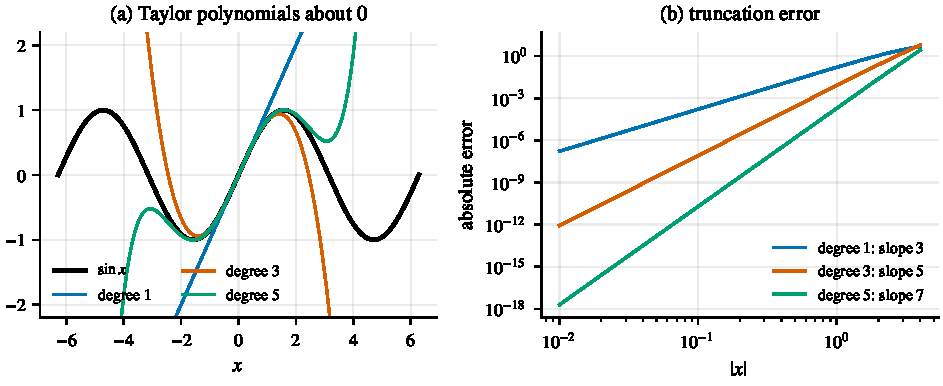
\includegraphics[width=0.95\textwidth]{fig_taylor_sin.pdf}
  \caption{Taylor polynomials of $\sin x$ about $0$ (left) and the absolute error of each (right, log-log scale). Near the expansion point the
  error of the degree-$n$ polynomial falls like $|x|^{n+1}$ or faster. Because the even-order terms of $\sin x$ vanish, the polynomials of degree 1, 3
  and 5 coincide with those of degree 2, 4 and 6, and their errors fall like $|x|^3$, $|x|^5$ and $|x|^7$ (slopes 3, 5 and 7). Far from the
  expansion point, every truncated series fails.}
  \label{fig:taylor-sin}
\end{figure}

\paragraph{Big-O and little-o.} We write $g(h) = O(h^p)$ if $|g(h)| \le Ch^p$ for some constant $C$ as $h\to0$, and $g(h) = o(h^p)$ if
$g(h)/h^p \to 0$. An approximation is \emph{first-order accurate} if its error is $O(h^2)$: the error of a linearization shrinks
quadratically with the size of the perturbation. ``Keeping terms to first order'' in a derivation means writing the result as
linear terms plus an $O(\|\delta\|^2)$ remainder, and then dropping the remainder.

For functions of several variables, Taylor's theorem to second order reads
\begin{equation}
  f(x + \delta) = f(x) + \nabla f(x)\T\delta + \tfrac12\delta\T\nabla^2f(x)\,\delta + O(\|\delta\|^3),
\end{equation}
and for vector functions each component expands this way. The size of the second-order term relative to the first measures how good a
linearization is: when uncertainties are small compared with the scale over which the Jacobian changes, linearization is accurate.
This is the quantitative content of the statement that an extended Kalman filter works well when errors are small (\cref{ch:nonlinear}).

\subsection{Matrix calculus}

A few derivatives recur throughout estimation. We write them as differentials ($\dd f$ = the linear change of $f$ for a small change of the
argument):
\begin{align}
  \dd(Ax) &= A\,\dd x, & \frac{\partial (Ax)}{\partial x} &= A, \\
  \dd(x\T Ax) &= x\T(A + A\T)\,\dd x, & \nabla_x(x\T Ax) &= (A + A\T)x \ \ (= 2Ax \text{ if } A \text{ symmetric}), \\
  \dd(a\times x) &= \sx{a}\,\dd x, & \dd(x \times a) &= -\sx{a}\,\dd x, \\
  \dd(A\inv) &= -A\inv(\dd A)A\inv, & \dd\log\det A &= \tr(A\inv\dd A) .
\end{align}
\begin{proof}[Derivations]
The first and third lines are linear maps, their own derivatives. For the quadratic form,
$(x + \dd x)\T A(x + \dd x) - x\T Ax = \dd x\T Ax + x\T A\,\dd x + O(\|\dd x\|^2) = x\T(A\T + A)\dd x + O(\|\dd x\|^2)$. For the inverse,
differentiate $AA\inv = I$: $(\dd A)A\inv + A\,\dd(A\inv) = 0$. For the log-determinant of a positive-definite $A = U\Lambda U\T$, a small
change $\dd A$ changes each eigenvalue by $u_i\T(\dd A)u_i$ to first order, so
$\dd\sum_i\log\lambda_i = \sum_iu_i\T(\dd A)u_i/\lambda_i = \tr(U\Lambda\inv U\T\dd A) = \tr(A\inv\dd A)$.
\end{proof}

\subsection{Stationary points}

A smooth function has a local minimum at $x^\star$ only if $\nabla f(x^\star) = 0$, and it does have one if, in addition,
$\nabla^2f(x^\star) \succ 0$: by the second-order Taylor expansion, $f(x^\star + \delta) - f(x^\star) = \tfrac12\delta\T\nabla^2f\,\delta + O(\|\delta\|^3) > 0$
for small $\delta \neq 0$. Every least-squares problem in these notes is solved by setting a gradient to zero; \cref{ch:nlls} develops the
iterative methods needed when the resulting equations are nonlinear.

% ==============================================================================
\section{Ordinary differential equations}

\subsection{What a differential equation is}

An \term{ordinary differential equation} (ODE) in state-space form is
\begin{equation}
  \dot x(t) = f\big(x(t), t\big), \qquad x(t_0) = x_0,
\end{equation}
where $x(t) \in \R^n$ is the \emph{state} and $\dot x = \dd x/\dd t$. Any higher-order equation can be put in this form by adding derivatives to
the state: Newton's law $\ddot p = a$ becomes the first-order system $\dot p = v$, $\dot v = a$ with state $(p, v)$. The kinematics of a
navigating vehicle are exactly such a system, with the IMU supplying the right-hand side.

\begin{theorem}[Existence and uniqueness, Picard--Lindel\"of]
\index{Picard--Lindel\"of theorem}
If $f$ is continuous in $t$ and Lipschitz continuous in $x$ (there is an $L$ with $\|f(x, t) - f(y, t)\| \le L\|x - y\|$), the initial value
problem has a unique solution on some interval around $t_0$.
\end{theorem}

Uniqueness is what makes prediction possible: the present state and the inputs determine the future. All the systems in these notes are
smooth enough for the theorem to apply. (A non-example is $\dot x = \sqrt{|x|}$, $x(0) = 0$, solved both by $x \equiv 0$ and by $x = t^2/4$.)

\subsection{Scalar linear equations}

The scalar equation $\dot x = ax + b(t)$ is solved with an \emph{integrating factor}. Multiplying by $e^{-at}$ gives
$\frac{\dd}{\dd t}\big(e^{-at}x\big) = e^{-at}b(t)$; integrating from $t_0$ to $t$,
\begin{equation}
  x(t) = e^{a(t - t_0)}x_0 + \int_{t_0}^t e^{a(t - s)}\,b(s)\,\dd s .
\end{equation}
The solution is the free response of the initial condition plus a weighted sum of the inputs, each propagated from the time it was applied.
Every linear system has this structure.

\subsection{Linear time-invariant systems}

\begin{theorem}[Solution of linear time-invariant systems]
\label{thm:lti-solution}
The solution of $\dot x = Ax + Bu(t)$, $x(t_0) = x_0$, is
\begin{equation}
  x(t) = e^{A(t - t_0)}x_0 + \int_{t_0}^t e^{A(t - s)}Bu(s)\,\dd s .
  \label{eq:lti-solution}
\end{equation}
In particular $\dot x = Ax$ has the unique solution $x(t) = e^{A(t - t_0)}x_0$.
\end{theorem}
\begin{proof}
By \cref{prop:matexp}, $\frac{\dd}{\dd t}\big(e^{-At}x\big) = e^{-At}(\dot x - Ax) = e^{-At}Bu$. Integrating from $t_0$ to $t$ and multiplying by $e^{At}$ gives
\eqref{eq:lti-solution}. The same computation shows that \emph{any} solution satisfies \eqref{eq:lti-solution}, which proves uniqueness.
\end{proof}

The matrix $e^{A\Dt}$ propagates the state over an interval $\Dt$. If $A = V\Lambda V\inv$, the solution is a combination of modes
$e^{\lambda_it}$: decaying for $\operatorname{Re}\lambda_i < 0$, growing for $\operatorname{Re}\lambda_i > 0$, oscillating for imaginary parts. Error
dynamics of inertial navigation have eigenvalues at zero, so their errors grow polynomially rather than exponentially
(\cref{ch:errordyn}).

\subsection{Linear time-varying systems and the state transition matrix}

When the system matrix changes with time, $\dot x = A(t)x$, the exponential no longer applies directly, but its key property survives.

\begin{definition}[State transition matrix]
\index{state transition matrix}
The \term{state transition matrix} $\Phi(t, s)$ of $\dot x = A(t)x$ is the solution of the matrix equation
$\frac{\partial}{\partial t}\Phi(t, s) = A(t)\Phi(t, s)$ with $\Phi(s, s) = I$.
\end{definition}

\begin{proposition}[Properties of the state transition matrix]
\label{prop:stm}
\begin{enumerate}
  \item $x(t) = \Phi(t, s)\,x(s)$ for every solution: $\Phi$ maps states at time $s$ to states at time $t$.
  \item $\Phi(t, s)\,\Phi(s, r) = \Phi(t, r)$ (the semigroup property) and $\Phi(t, s)\inv = \Phi(s, t)$.
  \item For constant $A$, $\Phi(t, s) = e^{A(t - s)}$.
  \item If $A(t)$ commutes with $A(s)$ for all $t, s$, then $\Phi(t, s) = \exp\big(\int_s^tA(\tau)\,\dd\tau\big)$. In general this formula is
        \emph{wrong}.
  \item The solution of $\dot x = A(t)x + B(t)u(t)$ is $x(t) = \Phi(t, t_0)x_0 + \int_{t_0}^t\Phi(t, s)B(s)u(s)\,\dd s$.
\end{enumerate}
\end{proposition}
\begin{proof}
(1) Both $x(t)$ and $\Phi(t, s)x(s)$ solve the ODE with the same value at $t = s$; by uniqueness they agree. (2) Both sides of the first
identity, as functions of $t$, solve the matrix ODE with the value $\Phi(s, r)$ at $t = s$. Setting $r = t$ gives the second. (3) Check that
$e^{A(t-s)}$ satisfies the definition. (4) If the $A(\tau)$ commute, so do $A(t)$ and $M(t) = \int_s^tA$, and then
$\frac{\dd}{\dd t}e^{M(t)} = A(t)e^{M(t)}$ by the commuting case of the series; without commutativity this derivative formula fails.
(5) Differentiate the right-hand side and use (1) and $\frac{\partial}{\partial t}\Phi = A\Phi$.
\end{proof}

Property 4 matters for attitude. The kinematics $\dot R = R\sx{\omega(t)}$ is a linear matrix ODE, and when the angular velocity changes
direction over time the rotation is \emph{not} $\exp\big(\int\sx{\omega}\big)$: rotations about different axes do not commute. Integrating
the angular velocity vector and exponentiating the result produces the ``coning'' error of \cref{ch:strapdown}.

A general series for $\Phi$, the \emph{Peano--Baker series}
\begin{equation*}
  \Phi(t,s) = I + \int_s^tA(\tau_1)\,\dd\tau_1 + \int_s^t\int_s^{\tau_1}A(\tau_1)A(\tau_2)\,\dd\tau_2\,\dd\tau_1 + \cdots,
\end{equation*}
obtained by repeatedly substituting the integral form of the ODE into itself, shows how products of non-commuting matrices enter. In practice $\Phi$ is approximated over short
intervals, where $A$ is nearly constant: $\Phi(t + \Dt, t) \approx \exp(A(t)\Dt) \approx I + A(t)\Dt$, the discretization used by every
filter in these notes.

% ==============================================================================
\section{Numerical integration of ODEs}
\label{sec:numint}

\subsection{Euler's method}

Truncating the Taylor expansion $x(t + h) = x(t) + h\dot x(t) + O(h^2)$ gives \term{Euler's method}:
\begin{equation}
  x_{k+1} = x_k + h\,f(x_k, t_k).
\end{equation}
Each step makes a \emph{local truncation error} of $O(h^2)$. Over a fixed interval $T$ there are $T/h$ steps, so one expects a
\emph{global error} of $O(h)$. The following proposition makes this precise; it also explains why local errors do not simply add up,
but can be amplified by the dynamics.

\begin{proposition}[Global error of Euler's method]
\index{Euler's method}
If $f$ is Lipschitz with constant $L$ and the exact solution has a bounded second derivative $\|\ddot x\| \le M$, the error
$e_k = x_k - x(t_k)$ of Euler's method satisfies $\|e_k\| \le \frac{Mh}{2L}\big(e^{L(t_k - t_0)} - 1\big)$.
\end{proposition}
\begin{proof}
The exact solution satisfies $x(t_{k+1}) = x(t_k) + hf(x(t_k)) + \tau_k$ with $\|\tau_k\| \le Mh^2/2$ by Taylor's theorem. Subtracting from the
numerical step, $e_{k+1} = e_k + h\big(f(x_k) - f(x(t_k))\big) - \tau_k$, so $\|e_{k+1}\| \le (1 + hL)\|e_k\| + Mh^2/2$. With $e_0 = 0$, induction gives
$\|e_k\| \le \frac{Mh^2}{2}\sum_{j<k}(1 + hL)^j = \frac{Mh}{2L}\big((1 + hL)^k - 1\big) \le \frac{Mh}{2L}\big(e^{Lkh} - 1\big)$.
\end{proof}

\begin{definition}[Order of a method]
A method has \emph{order} $p$ if its global error over a fixed interval is $O(h^p)$; equivalently its local error is $O(h^{p+1})$.
\end{definition}

\subsection{Higher-order methods}

\emph{Runge--Kutta} methods evaluate $f$ at several points inside the step and combine the results so that the Taylor expansion of the step
matches the true solution to higher order.
\begin{itemize}
  \item \textbf{Midpoint method} (order 2): $k_1 = f(x_k, t_k)$, $x_{k+1} = x_k + hf(x_k + \tfrac h2k_1, t_k + \tfrac h2)$.
  \item \textbf{Heun's method / trapezoidal rule} (order 2): $k_1 = f(x_k, t_k)$, $k_2 = f(x_k + hk_1, t_k + h)$,
        $x_{k+1} = x_k + \tfrac h2(k_1 + k_2)$.
  \item \textbf{Classical RK4} (order 4): $k_1 = f(x_k, t_k)$, $k_2 = f(x_k + \tfrac h2k_1, t_k + \tfrac h2)$,
        $k_3 = f(x_k + \tfrac h2k_2, t_k + \tfrac h2)$, $k_4 = f(x_k + hk_3, t_k + h)$, $x_{k+1} = x_k + \tfrac h6(k_1 + 2k_2 + 2k_3 + k_4)$.
\end{itemize}
Verifying the order means expanding both the numerical step and the exact solution in Taylor series and comparing coefficients. For Heun's
method on $\dot x = f(x)$: $k_2 = f(x + hf) = f + hf'f + O(h^2)$, so the step is $x + hf + \tfrac{h^2}2f'f + O(h^3)$, which matches
$x(t + h) = x + h\dot x + \tfrac{h^2}2\ddot x + O(h^3)$ because $\ddot x = f'f$.

\begin{figure}[t]
  \centering
  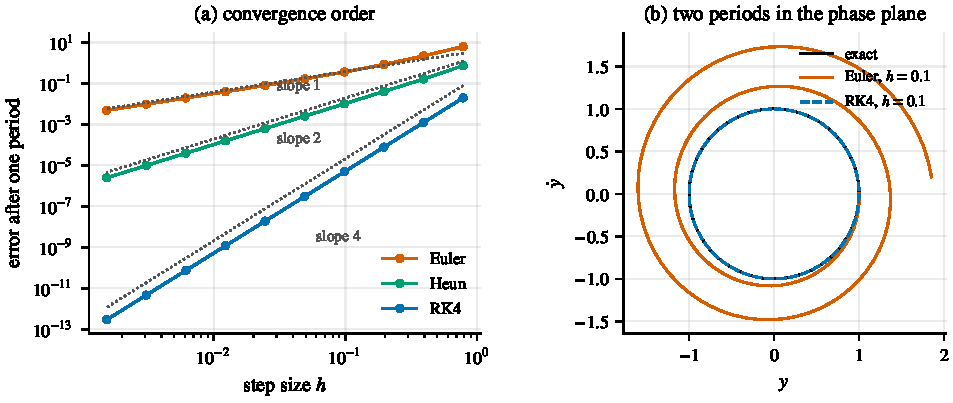
\includegraphics[width=\textwidth]{fig_ode_methods.pdf}
  \caption{Integrating the harmonic oscillator $\ddot y = -y$. (a) Global error after one period versus step size: slopes 1, 2 and 4 confirm the
  orders of Euler, Heun and RK4. (b) With $h = 0.1$, Euler's method spirals outward, gaining energy every step, while RK4 stays on the
  circle to plotting accuracy.}
  \label{fig:ode-methods}
\end{figure}

\paragraph{Verifying the order.} If the error behaves as $Ch^p$, then halving the step divides the error by $2^p$, and the order can be
\emph{measured}: $p \approx \log_2\big(e(h)/e(h/2)\big)$. \Cref{fig:ode-methods}(a) shows this for three methods. A convergence-order test of
this kind is one of the most powerful tests of an integrator: an implementation bug almost always destroys the expected order
(Milestone 4).

\paragraph{Stability.} Euler's method applied to the decaying equation $\dot x = -\lambda x$ gives $x_{k+1} = (1 - h\lambda)x_k$, which blows up
when $h > 2/\lambda$, although the true solution decays. Stiff systems, with very fast decaying modes, need tiny steps or implicit methods.
Applied to an oscillator, Euler's method multiplies the amplitude by $\sqrt{1 + h^2\omega^2} > 1$ per step and spirals outward
(\cref{fig:ode-methods}b). Inertial navigation is not stiff, but this effect is the reason a naive attitude integrator slowly inflates the
norm of its rotation matrix, as we now see.

\subsection{Integrating on a curved space}
\label{sec:lie-euler}

Apply Euler's method to the attitude kinematics $\dot R = R\sx{\omega}$: $R_{k+1} = R_k + hR_k\sx{\omega} = R_k(I + h\sx{\omega})$. The result
is not a rotation matrix:
\begin{equation}
  (I + h\sx{\omega})\T(I + h\sx{\omega}) = I - h^2\sx{\omega}^2 \neq I,
\end{equation}
so every step stretches vectors perpendicular to $\omega$ by a factor of about $1 + \tfrac12h^2\|\omega\|^2$, and the matrix drifts off the set of
rotations. The remedy is to integrate in a way that respects the structure of the space. For constant $\omega$ over the step, the exact
solution is $R_k\exp(h\sx{\omega})$ (\cref{thm:lti-solution}), so the \emph{Lie--Euler} method
\begin{equation}
  R_{k+1} = R_k\exp(h\sx{\omega_k})
\end{equation}
stays exactly on the set of rotations (\cref{prop:exp-skew}) and is first order in general, exact when $\omega$ is constant. Higher-order
generalizations (Runge--Kutta--Munthe-Kaas methods) apply Runge--Kutta to a vector-space parameterization of the increment. Every attitude
update in these notes is multiplicative in this sense (AGENTS.md F1).

% ==============================================================================
\section{Numerical differentiation}
\label{sec:numdiff}

Analytic Jacobians are derived by hand and verified numerically (AGENTS.md E6). Numerical differentiation is easy to write and easy to
get subtly wrong, because it is a subtraction of nearly equal numbers.

\paragraph{Forward differences.} By Taylor's theorem,
\begin{equation}
  \frac{f(x + h) - f(x)}{h} = f'(x) + \frac h2f''(\xi),
\end{equation}
so the \emph{truncation error} is about $\frac h2|f''|$. But $f(x + h)$ and $f(x)$ are each computed with a rounding error of about $u|f|$, and
their difference is divided by $h$, which adds a \emph{rounding error} of about $2u|f|/h$. The total $\frac h2|f''| + \frac{2u|f|}{h}$ is minimized at
$h^\star = 2\sqrt{u|f|/|f''|} \approx 10^{-8}$ for quantities of order one, with a total error of about $10^{-8}$.

\paragraph{Central differences.} Expanding both $f(x \pm h)$,
\begin{equation}
  \frac{f(x + h) - f(x - h)}{2h} = f'(x) + \frac{h^2}{6}f'''(\xi),
\end{equation}
because the even-order terms cancel. The total error $\frac{h^2}6|f'''| + \frac{u|f|}{h}$ is minimized at
\begin{equation}
  h^\star = \left(\frac{3\,u\,|f|}{|f'''|}\right)^{1/3} \approx 10^{-5}\text{ to }10^{-6},
\end{equation}
with a total error of order $u^{2/3} \approx 10^{-11}$.

\begin{figure}[t]
  \centering
  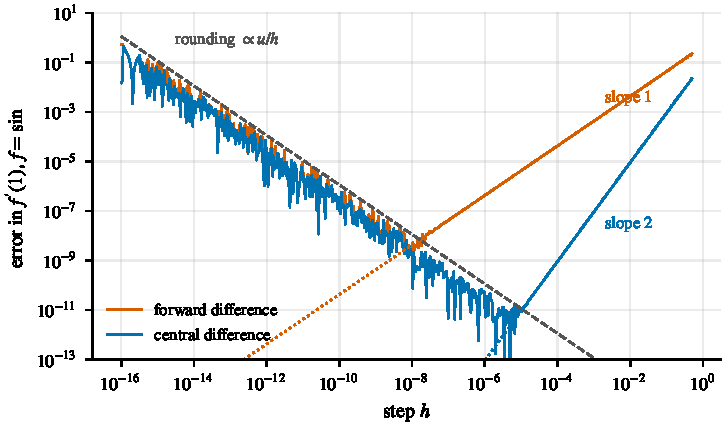
\includegraphics[width=0.85\textwidth]{fig_fd_error.pdf}
  \caption{Error of finite-difference derivatives of $\sin x$ at $x = 1$ versus step size. To the right of the optimum, truncation error
  dominates (slopes 1 and 2); to the left, rounding error grows like $u/h$. Central differences reach about $10^{-11}$; forward differences
  only about $10^{-8}$.}
  \label{fig:fd-error}
\end{figure}

\Cref{fig:fd-error} shows both error regimes. This is why the Jacobian tests of the project use central differences with $h \approx 10^{-6}$
and tolerances of about $10^{-6}$ to $10^{-8}$ relative to the size of the entries. A tolerance tighter than the achievable accuracy makes a
correct implementation fail; a much looser one lets a wrong implementation pass.

\paragraph{Jacobians.} For $f: \R^n \to \R^m$, column $j$ of the numerical Jacobian is
$\big(f(x + he_j) - f(x - he_j)\big)/2h$, costing $2n$ evaluations of $f$. On manifolds the perturbation and the difference are replaced by
$\bplus$ and $\bminus$ (\cref{ch:lie}); nothing else changes.

\begin{aside}[the complex-step derivative]
If $f$ is analytic and can be evaluated with complex arguments, $f'(x) = \operatorname{Im}f(x + ih)/h + O(h^2)$, with no subtraction at all.
With $h = 10^{-20}$ the result is exact to machine precision. The technique requires that every operation in $f$ be implemented for complex
numbers and avoid non-analytic functions (absolute values, comparisons), which rules it out for most estimator code. It is a superb way to
generate reference Jacobians in Python, though.
\end{aside}

\begin{takeaways}
\begin{itemize}
  \item The Jacobian is the matrix of the best linear approximation; the chain rule multiplies Jacobians in composition order.
  \item Taylor's theorem bounds approximation errors. ``First order'' means an error of $O(\|\delta\|^2)$.
  \item $\dd(A\inv) = -A\inv\dd A\,A\inv$ and $\dd\log\det A = \tr(A\inv\dd A)$.
  \item $\dot x = Ax + Bu$ is solved by $e^{At}$ plus a convolution of the inputs; time-varying systems use the state transition matrix,
        which is \emph{not} the exponential of the integrated system matrix unless the matrices commute.
  \item A method of order $p$ has global error $O(h^p)$; halving the step should divide the error by $2^p$. Measure it.
  \item Euler's method leaves the set of rotations; multiplicative updates $R\exp(h\sx{\omega})$ do not.
  \item Central differences with $h \approx 10^{-6}$ reach about $10^{-11}$ accuracy; forward differences only about $10^{-8}$.
\end{itemize}
\end{takeaways}

\begin{exercises}
  \item Compute the Jacobian of $f(x, y) = (x^2y, \sin(xy), e^x)$ and verify it with central differences.
  \item Use Taylor's theorem to bound the error of $\cos h \approx 1 - h^2/2$ for $|h| \le 0.1$.
  \item Show that $\nabla_x\|Ax - b\|^2 = 2A\T(Ax - b)$ and $\nabla_x^2\|Ax - b\|^2 = 2A\T A$.
  \item Solve $\dot x = -2x + 1$, $x(0) = 3$, and check the solution by substitution.
  \item For $A = \begin{bmatrix}0 & 1\\ -1 & 0\end{bmatrix}$, compute $e^{At}$ and interpret the solution of $\dot x = Ax$.
  \item Find the state transition matrix of $\dot x = \begin{bmatrix}0 & t\\0 & 0\end{bmatrix}x$. Do the matrices $A(t)$ commute?
  \item Construct two angular velocity profiles with the same integral $\int\omega\,\dd t$ that produce different final rotations.
  \item Implement Euler, Heun and RK4 for the harmonic oscillator and reproduce \cref{fig:ode-methods}(a).
  \item Show that one Euler step on $\dot R = R\sx{\omega}$ increases $\det R$ by a factor $1 + h^2\|\omega\|^2$, to leading order.
  \item Reproduce \cref{fig:fd-error} and compare the observed optimal step sizes with the formulas of \cref{sec:numdiff}.
\end{exercises}
\input{chapters/solutions/04_calculus_odes}

\chapter{Probability and Random Vectors}
\label{ch:prob}

\begin{objectives}
\begin{itemize}
  \item Build probability from its axioms: conditional probability, independence and Bayes' rule.
  \item Work with random variables and random vectors: densities, expectations, covariances and changes of variables.
  \item Derive the Gaussian distribution and its key properties: affine maps, marginals, conditionals and the fusion of estimates.
  \item Understand the law of large numbers, the central limit theorem and Monte Carlo methods.
  \item Derive the $\chi^2$ distribution and use it for hypothesis tests, the basis of gating and consistency checks.
  \item Understand how nonlinear functions distort distributions, and what linearization keeps and loses.
\end{itemize}
\end{objectives}

A filter does not merely estimate the state; it maintains a probability distribution over it. The estimate is the center of
that distribution, and the covariance describes its spread. This chapter develops the probability theory that gives these words a
precise meaning.

% ==============================================================================
\section{Probability}

\subsection{Events and the axioms}

A random experiment has a set $\Omega$ of possible outcomes, the \term{sample space}. An \term{event} is a subset of outcomes, and a
\term{probability} assigns to each event $A$ a number $P(A)$ obeying three axioms (Kolmogorov):
\begin{enumerate}
  \item $P(A) \ge 0$ for every event;
  \item $P(\Omega) = 1$;
  \item if $A_1, A_2, \dots$ are mutually exclusive (pairwise disjoint), $P(A_1\cup A_2\cup\cdots) = \sum_iP(A_i)$.
\end{enumerate}
Everything else follows: $P(\text{not }A) = 1 - P(A)$, $P(A\cup B) = P(A) + P(B) - P(A\cap B)$, and so on. Probability can be read as a
long-run frequency (the fraction of repetitions in which $A$ occurs) or as a degree of belief; the mathematics is the same, and filters
use both readings.

\subsection{Conditional probability and independence}

\begin{definition}[Conditional probability]
For $P(B) > 0$, the probability of $A$ given $B$ is $P(A\mid B) = P(A\cap B)/P(B)$.
\end{definition}

Conditioning restricts attention to the outcomes in which $B$ happened and renormalizes. Two events are \term{independent} if
$P(A\cap B) = P(A)P(B)$, equivalently $P(A\mid B) = P(A)$: knowing that $B$ occurred tells nothing about $A$.

\begin{proposition}[Law of total probability and Bayes' rule]
\index{Bayes' rule}
If $B_1, \dots, B_n$ are mutually exclusive and cover $\Omega$, then $P(A) = \sum_iP(A\mid B_i)P(B_i)$, and
\begin{equation}
  P(B_i\mid A) = \frac{P(A\mid B_i)\,P(B_i)}{\sum_jP(A\mid B_j)\,P(B_j)} .
\end{equation}
\end{proposition}
\begin{proof}
$A$ is the disjoint union of the $A\cap B_i$, and $P(A\cap B_i) = P(A\mid B_i)P(B_i)$. Bayes' rule is the definition of conditional
probability applied twice: $P(B_i\mid A)P(A) = P(A\cap B_i) = P(A\mid B_i)P(B_i)$.
\end{proof}

Bayes' rule turns the probability of an observation given a hypothesis (which a sensor model provides) into the probability of the
hypothesis given the observation (which we want).

\begin{worked}[how informative is a passed test?]
Suppose 10\% of the feature tracks reaching an outlier test are wrong. The test rejects 90\% of wrong tracks, and (being a 95\% gate)
also rejects 5\% of correct ones. A track passes. What is the probability that it is wrong? With $W$ = ``wrong'' and $A$ = ``passes'':
$P(A\mid W) = 0.1$, $P(W) = 0.1$, $P(A\mid\text{correct}) = 0.95$, $P(\text{correct}) = 0.9$. Bayes' rule gives
\begin{equation*}
  P(W\mid A) = \frac{0.1\times0.1}{0.1\times0.1 + 0.95\times0.9} = \frac{0.01}{0.865} \approx 1.2\% .
\end{equation*}
The test reduces the outlier fraction from 10\% to about 1\%: very useful, but not perfect, which is why the estimator adds further
checks downstream.
\end{worked}

% ==============================================================================
\section{Random variables}

\subsection{Distributions, densities and expectations}

A \term{random variable} $X$ is a numerical quantity determined by the outcome of an experiment. Its \emph{cumulative distribution
function} is $F(x) = P(X \le x)$. A discrete random variable takes countably many values with probabilities $p(x) = P(X = x)$; a continuous
one has a \term{probability density function} (pdf) $p(x) \ge 0$ with
\begin{equation}
  P(a \le X \le b) = \int_a^bp(x)\,\dd x, \qquad \int_{-\infty}^\infty p(x)\,\dd x = 1 .
\end{equation}
A density is not a probability: $p(x)\,\dd x$ is the probability of falling in a small interval of width $\dd x$ around $x$, and a density
can exceed one.

\begin{definition}[Expectation and variance]
The \term{expectation} (mean) of $X$ is $\E[X] = \int x\,p(x)\,\dd x$ (a sum for discrete variables). The expectation of a function of $X$ is
$\E[g(X)] = \int g(x)p(x)\,\dd x$. The \term{variance} is $\Var(X) = \E[(X - \E X)^2] = \E[X^2] - (\E X)^2$, and its square root is the
\term{standard deviation} $\sigma$.
\end{definition}

Expectation is linear: $\E[aX + bY + c] = a\E[X] + b\E[Y] + c$ for any random variables, dependent or not. Variance scales quadratically and
ignores shifts: $\Var(aX + c) = a^2\Var(X)$. The standard deviation has the units of $X$ and measures its typical spread.

\begin{example}[Uniform distribution]
$X$ uniform on $[a, b]$ has $p(x) = 1/(b - a)$ there, mean $(a + b)/2$ and variance $(b - a)^2/12$. Rounding a reading to a resolution
$\Delta$ produces an error that is approximately uniform on $[-\Delta/2, \Delta/2]$, with standard deviation $\Delta/\sqrt{12}$: the
quantization noise of a sensor.
\end{example}

\subsection{The Gaussian distribution}

\begin{definition}[Gaussian distribution]
\index{Gaussian distribution}
$X \sim \N(\mu, \sigma^2)$ has density
\begin{equation}
  p(x) = \frac{1}{\sqrt{2\pi}\,\sigma}\exp\!\Big(-\frac{(x - \mu)^2}{2\sigma^2}\Big).
\end{equation}
The \emph{standard normal} distribution is $\N(0, 1)$.
\end{definition}

\begin{proposition}[Normalization]
$\int_{-\infty}^\infty e^{-x^2/2}\,\dd x = \sqrt{2\pi}$.
\end{proposition}
\begin{proof}
Let $I$ be the integral. Then $I^2 = \iint e^{-(x^2 + y^2)/2}\,\dd x\,\dd y$. In polar coordinates, with area element $r\,\dd r\,\dd\theta$,
$I^2 = \int_0^{2\pi}\!\int_0^\infty e^{-r^2/2}r\,\dd r\,\dd\theta = 2\pi\big[-e^{-r^2/2}\big]_0^\infty = 2\pi$.
\end{proof}

Substituting $x \to (x - \mu)/\sigma$ shows that the general density integrates to one, and similar integrals (using symmetry and
integration by parts) give $\E[X] = \mu$ and $\Var(X) = \sigma^2$. If $X \sim \N(\mu, \sigma^2)$ then $(X - \mu)/\sigma \sim \N(0, 1)$, and the
probabilities of falling within one, two and three standard deviations of the mean are $68.27\%$, $95.45\%$ and $99.73\%$. A Gaussian is
completely determined by its mean and variance, and is closed under the operations a linear filter performs, which is why Kalman
filters can work with means and covariances alone.

% ==============================================================================
\section{Several random variables}

\subsection{Joint, marginal and conditional densities}

Two random variables $X, Y$ have a \emph{joint density} $p(x, y)$, with $P((X, Y) \in A) = \iint_Ap(x, y)\,\dd x\,\dd y$. From it:
\begin{align}
  \text{marginal:}&\quad p(x) = \int p(x, y)\,\dd y, \\
  \text{conditional:}&\quad p(x\mid y) = \frac{p(x, y)}{p(y)}, \\
  \text{Bayes' rule:}&\quad p(x\mid y) = \frac{p(y\mid x)\,p(x)}{p(y)} = \frac{p(y\mid x)\,p(x)}{\int p(y\mid x')p(x')\,\dd x'} .
\end{align}
$X$ and $Y$ are independent if $p(x, y) = p(x)p(y)$. In estimation, $x$ is the unknown state and $y$ the measurement: $p(y\mid x)$ is the
sensor model (the \emph{likelihood}), $p(x)$ is the \emph{prior}, and $p(x\mid y)$ the \emph{posterior}.

\subsection{Covariance and correlation}

The \term{covariance} $\Cov(X, Y) = \E[(X - \E X)(Y - \E Y)]$ measures how two variables vary together, and the \term{correlation
coefficient} $\rho = \Cov(X, Y)/(\sigma_X\sigma_Y) \in [-1, 1]$ normalizes it (the bound is the Cauchy--Schwarz inequality). Independent
variables have zero covariance, and then $\Var(X + Y) = \Var(X) + \Var(Y)$: variances of independent errors add.

The converse fails: zero correlation does not imply independence. If $X \sim \N(0, 1)$ and $Y = X^2$, then $\Cov(X, Y) = \E[X^3] = 0$, yet $Y$
is a function of $X$. Correlation measures only \emph{linear} dependence. (For jointly Gaussian variables the converse does hold, as shown
below.)

% ==============================================================================
\section{Random vectors}

\subsection{Mean and covariance}

For a random vector $x \in \R^n$ with density $p(x)$, the mean and \term{covariance matrix} are
\begin{equation}
  \mu = \E[x], \qquad \Sigma = \Cov(x) = \E\big[(x - \mu)(x - \mu)\T\big] = \E[xx\T] - \mu\mu\T .
\end{equation}
The diagonal of $\Sigma$ holds the variances $\sigma_i^2$ and its off-diagonal entries the covariances. $\Sigma$ is symmetric and positive
semi-definite: for any fixed $a$, $a\T\Sigma a = \E\big[(a\T(x - \mu))^2\big] \ge 0$. The \emph{cross-covariance} of two random vectors is
$\Sigma_{xy} = \E[(x - \mu_x)(y - \mu_y)\T]$, and $\Sigma_{yx} = \Sigma_{xy}\T$.

\begin{proposition}[Affine transformations]
\label{prop:affine}
If $y = Ax + b$ then $\E[y] = A\mu + b$ and $\Cov(y) = A\Sigma A\T$. If $x$ and $w$ are uncorrelated, $\Cov(Ax + Bw) = A\Sigma_xA\T + B\Sigma_wB\T$.
\end{proposition}
\begin{proof}
Linearity of expectation gives the mean. Then $\Cov(y) = \E[A(x - \mu)(x - \mu)\T A\T] = A\Sigma A\T$. With uncorrelated $x$ and $w$, the cross terms
$A\Sigma_{xw}B\T$ vanish.
\end{proof}

This one proposition is the covariance propagation of the Kalman filter ($P \leftarrow \Phi P \Phi\T + Q$), the covariance of a stacked
measurement, and the augmentation formula of stochastic cloning ($P \leftarrow JPJ\T$).

\begin{proposition}[Expected value of a quadratic form]
\label{prop:quadratic-expectation}
For any matrix $A$, $\E[x\T Ax] = \tr(A\Sigma) + \mu\T A\mu$. In particular, if $\mu = 0$ then $\E[x\T\Sigma\inv x] = \tr(I_n) = n$.
\end{proposition}
\begin{proof}
$x\T Ax = \tr(Axx\T)$, and expectation commutes with the trace: $\E[x\T Ax] = \tr(A\,\E[xx\T]) = \tr(A(\Sigma + \mu\mu\T))$.
\end{proof}

The special case is the reason a consistent filter's normalized estimation error squared averages to the dimension of the state
(\cref{ch:consistency}).

\subsection{Changing variables}

\begin{proposition}[Change of variables]
\label{prop:change-of-variables}
If $y = g(x)$ with $g$ invertible and differentiable, the densities are related by
$p_y(y) = p_x\big(g\inv(y)\big)\,\big|\det\frac{\partial g\inv}{\partial y}\big|$.
\end{proposition}

In one dimension this follows from equating probabilities of corresponding small intervals, $p_y(y)\,|\dd y| = p_x(x)\,|\dd x|$; in several
dimensions the determinant measures how $g\inv$ stretches volumes (\cref{sec:determinants}). For an invertible linear map $y = Ax$ the factor
is the constant $1/|\det A|$.

% ==============================================================================
\section{The multivariate Gaussian}

\subsection{Definition}

\begin{definition}[Multivariate Gaussian]
\index{Gaussian distribution!multivariate}
A random vector $x \in \R^n$ is Gaussian, $x \sim \N(\mu, \Sigma)$, if it can be written as $x = \mu + Ls$ where $s$ has independent standard
normal components and $LL\T = \Sigma$. If $\Sigma \succ 0$ its density is
\begin{equation}
  p(x) = \frac{1}{\sqrt{(2\pi)^n \det\Sigma}}\exp\!\Big( -\tfrac12 (x - \mu)\T \Sigma\inv (x - \mu) \Big).
  \label{eq:gaussian-pdf}
\end{equation}
The quantity $d_M^2(x) = (x - \mu)\T\Sigma\inv(x - \mu)$ is the squared \term{Mahalanobis distance} of $x$ from the mean.
\end{definition}

\begin{proof}[Derivation of the density]
The density of $s$ is the product of $n$ standard normal densities, $(2\pi)^{-n/2}\exp(-\tfrac12s\T s)$. By \cref{prop:change-of-variables} with
$s = L\inv(x - \mu)$, $p(x) = (2\pi)^{-n/2}\exp\big(-\tfrac12(x - \mu)\T L\mT L\inv(x - \mu)\big)/|\det L|$. Since $L\mT L\inv = (LL\T)\inv = \Sigma\inv$ and
$|\det L| = \sqrt{\det\Sigma}$, this is \eqref{eq:gaussian-pdf}.
\end{proof}

By \cref{prop:affine}, the mean of $x$ is $\mu$ and its covariance is $L\,\E[ss\T]L\T = \Sigma$. The definition also handles singular
covariances (with $L$ not invertible), which arise naturally in stochastic cloning (\cref{ch:cloning}).

\begin{figure}[t]
  \centering
  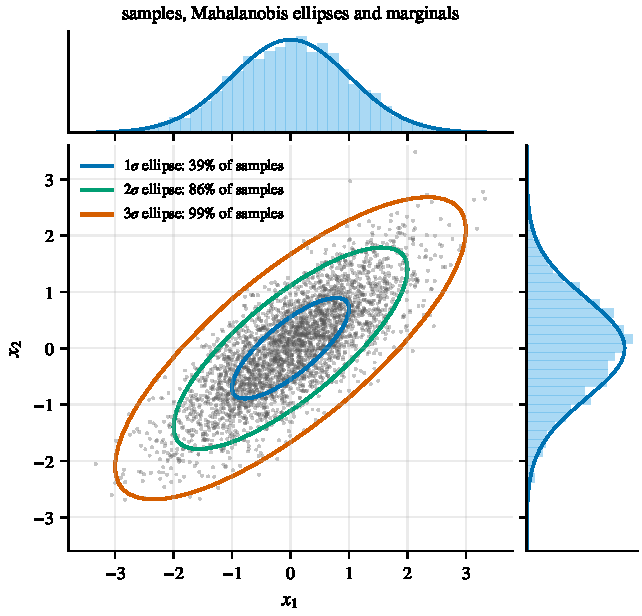
\includegraphics[width=0.92\textwidth]{fig_gauss2d.pdf}
  \caption{Samples of a correlated 2D Gaussian with the $1\sigma$, $2\sigma$ and $3\sigma$ Mahalanobis ellipses, and the two marginal densities.
  The ellipses are aligned with the eigenvectors of $\Sigma$. In two dimensions they contain 39\%, 86\% and 99\% of the probability, not
  the familiar 68--95--99.7\% of one dimension.}
  \label{fig:gauss2d}
\end{figure}

\paragraph{Geometry.} The density is constant on the ellipsoids $d_M^2(x) = c$, whose axes point along the eigenvectors of $\Sigma$ with lengths
proportional to the square roots of its eigenvalues (\cref{fig:ellipse,fig:gauss2d}). The Mahalanobis distance measures distance in units of
standard deviations along each principal axis, which makes it the natural way to ask whether a vector is ``far'' from a distribution.

\paragraph{Sampling.} To draw from $\N(\mu, \Sigma)$, factor $\Sigma = LL\T$ (Cholesky), draw $s \sim \N(0, I)$, and return $\mu + Ls$. Monte Carlo tests
of covariance propagation (Milestone 5) use exactly this.

\paragraph{Closure.} Affine maps of Gaussian vectors are Gaussian (directly from the definition). Marginals, conditionals and products of
Gaussian densities are Gaussian (next section). Hence a Gaussian belief propagated through a linear system with Gaussian noise remains
exactly Gaussian, and the Kalman filter is exact in that case. For jointly Gaussian vectors, uncorrelated implies independent: if the
covariance is block diagonal, the density factors.

\paragraph{Information form.} A Gaussian can equally be parameterized by the \term{information matrix} $\Lambda = \Sigma\inv$ and the
\emph{information vector} $\eta = \Sigma\inv\mu$. Then $-\log p(x) = \tfrac12 x\T\Lambda x - \eta\T x + \text{const}$. The information form is natural
for combining independent pieces of evidence, since their information adds, and it is the form in which optimization-based estimators work.

\subsection{Marginals and conditionals}

Partition a jointly Gaussian vector as
\begin{equation}
  \begin{bmatrix} a \\ b \end{bmatrix} \sim
  \N\!\left( \begin{bmatrix} \mu_a \\ \mu_b \end{bmatrix},
  \begin{bmatrix} \Sigma_{aa} & \Sigma_{ab} \\ \Sigma_{ba} & \Sigma_{bb} \end{bmatrix} \right),
  \qquad
  \Lambda = \Sigma\inv = \begin{bmatrix} \Lambda_{aa} & \Lambda_{ab} \\ \Lambda_{ba} & \Lambda_{bb} \end{bmatrix}.
\end{equation}

\begin{theorem}[Gaussian marginalization and conditioning]
\label{thm:gauss-cond}
\index{marginalization}\index{conditioning}
\begin{enumerate}
  \item The marginal of $a$ is $\N(\mu_a, \Sigma_{aa})$.
  \item The conditional of $a$ given $b$ is $\N(\mu_{a|b}, \Sigma_{a|b})$ with
  \begin{equation}
    \mu_{a|b} = \mu_a + \Sigma_{ab}\Sigma_{bb}\inv (b - \mu_b), \qquad
    \Sigma_{a|b} = \Sigma_{aa} - \Sigma_{ab}\Sigma_{bb}\inv\Sigma_{ba}.
    \label{eq:gauss-cond}
  \end{equation}
\end{enumerate}
\end{theorem}
\begin{proof}
The marginal follows from \cref{prop:affine} with the selection matrix $A = [I\ \ 0]$. For the conditional, define
$\tilde a = a - \Sigma_{ab}\Sigma_{bb}\inv b$. Then $\Cov(\tilde a, b) = \Sigma_{ab} - \Sigma_{ab}\Sigma_{bb}\inv\Sigma_{bb} = 0$, so $\tilde a$ and $b$ are uncorrelated,
and being jointly Gaussian they are independent. By \cref{prop:affine},
$\tilde a \sim \N(\mu_a - \Sigma_{ab}\Sigma_{bb}\inv\mu_b,\ \Sigma_{aa} - \Sigma_{ab}\Sigma_{bb}\inv\Sigma_{ba})$. Conditioning on $b$ leaves the distribution of
$\tilde a$ unchanged (independence), and $a = \tilde a + \Sigma_{ab}\Sigma_{bb}\inv b$, which gives \eqref{eq:gauss-cond}.
\end{proof}

The conditional mean moves away from $\mu_a$ in proportion to how far $b$ is from its mean, by the ``regression'' matrix $\Sigma_{ab}\Sigma_{bb}\inv$,
and the conditional covariance shrinks by a positive semi-definite amount. It does not depend on the observed value of $b$, only on the
fact that it was observed. The conditional covariance is the Schur complement $\Sigma/\Sigma_{bb}$; applying \cref{prop:block-inverse} to $\Sigma$
shows that $\Lambda_{aa} = \Sigma_{a|b}\inv$ and that the marginal information matrix is a Schur complement of $\Lambda$. The two parameterizations
therefore swap the roles of the two operations:

\begin{center}\small
\begin{tabular}{@{}lll@{}}
\toprule
 & covariance form $(\mu, \Sigma)$ & information form $(\eta, \Lambda)$ \\
\midrule
marginalize out $b$ & $\Sigma_{aa}$ \hfill(\textbf{delete rows/columns}) & $\Lambda_{aa} - \Lambda_{ab}\Lambda_{bb}\inv\Lambda_{ba}$ \hfill(Schur compl.) \\
condition on $b$ & $\Sigma_{aa} - \Sigma_{ab}\Sigma_{bb}\inv\Sigma_{ba}$ \hfill(Schur compl.) & $\Lambda_{aa}$ \hfill(\textbf{delete rows/columns}) \\
\bottomrule
\end{tabular}
\end{center}

\begin{keyidea}[marginalization is free in covariance form]
A Kalman filter stores covariances, so discarding a variable (the oldest clone of the MSCKF window) is literally deleting its rows and
columns from $P$. Optimization-based estimators store information matrices, so the same operation requires a Schur complement, which
creates fill-in and the ``marginalization prior'' of sliding-window smoothers (\cref{ch:nlls}).
\end{keyidea}

% ==============================================================================
\section{Fusing information: Bayes' rule for Gaussians}

\subsection{Combining two estimates}

Suppose two independent sensors measure the same scalar $x$, with readings $z_1 = x + n_1$ and $z_2 = x + n_2$ and noise variances $\sigma_1^2$ and
$\sigma_2^2$. With no other knowledge of $x$, the posterior density is proportional to the product of the two likelihoods,
\begin{equation}
  p(x\mid z_1, z_2) \propto \exp\!\Big(-\frac{(x - z_1)^2}{2\sigma_1^2}\Big)\exp\!\Big(-\frac{(x - z_2)^2}{2\sigma_2^2}\Big).
\end{equation}
The exponent is a quadratic in $x$; completing the square shows that the posterior is Gaussian with
\begin{equation}
  \frac{1}{\sigma^2} = \frac1{\sigma_1^2} + \frac1{\sigma_2^2}, \qquad
  \hat x = \sigma^2\Big(\frac{z_1}{\sigma_1^2} + \frac{z_2}{\sigma_2^2}\Big) = z_1 + \frac{\sigma_1^2}{\sigma_1^2 + \sigma_2^2}(z_2 - z_1).
  \label{eq:fusion}
\end{equation}
\emph{Inverse variances (information) add}, and the fused estimate is an information-weighted average. The second form already has the shape
of a Kalman update: start from $z_1$ and correct it by a gain times the discrepancy $z_2 - z_1$, with a gain between 0 and 1 that is large
when the first estimate is poor. The fused variance is smaller than both, so combining independent information always helps.

\subsection{The linear-Gaussian model}

\begin{proposition}[Linear-Gaussian posterior]
\label{prop:map-ls}
If $x \sim \N(\mu, P)$ and $z = Hx + n$ with $n \sim \N(0, R)$ independent of $x$, the posterior $p(x\mid z)$ is Gaussian, and its mean (which is
also its mode) solves the weighted least-squares problem
\begin{equation}
  \hat x = \argmin_x\ \|x - \mu\|^2_{P\inv} + \|z - Hx\|^2_{R\inv},
  \qquad \|e\|^2_{W} := e\T W e .
  \label{eq:map-ls}
\end{equation}
Its covariance is $(P\inv + H\T R\inv H)\inv$.
\end{proposition}
\begin{proof}
By Bayes' rule $p(x\mid z) \propto p(z\mid x)p(x)$, and
$-\log p(x\mid z) = \tfrac12\|x - \mu\|^2_{P\inv} + \tfrac12\|z - Hx\|^2_{R\inv} + \text{const}$. This is a convex quadratic in $x$ whose quadratic term is
$\tfrac12x\T(P\inv + H\T R\inv H)x$, so the posterior is Gaussian with that information matrix, and its mode, which for a Gaussian is the mean,
minimizes the quadratic.
\end{proof}

This is the scalar fusion rule in matrix form: the prior contributes information $P\inv$, the measurement contributes $H\T R\inv H$, and they add.
\Cref{ch:estimation} develops this into the general theory of estimators, and \cref{ch:kf} turns it into the Kalman filter.

% ==============================================================================
\section{Limit theorems and Monte Carlo}

\subsection{The law of large numbers}

Let $X_1, X_2, \dots$ be independent draws from the same distribution, with mean $\mu$ and variance $\sigma^2$, and let
$\bar X_N = \frac1N\sum_{i=1}^NX_i$ be their \term{sample mean}. Then $\E[\bar X_N] = \mu$ and, because variances of independent terms add,
$\Var(\bar X_N) = \sigma^2/N$.

\begin{theorem}[Weak law of large numbers]
\index{law of large numbers}
For every $\epsilon > 0$, $P(|\bar X_N - \mu| > \epsilon) \to 0$ as $N\to\infty$.
\end{theorem}
\begin{proof}
Chebyshev's inequality $P(|Y - \E Y| \ge \epsilon) \le \Var(Y)/\epsilon^2$ (which follows from
$\Var(Y) \ge \E[(Y - \E Y)^2\,\mathbf 1_{|Y - \E Y|\ge\epsilon}] \ge \epsilon^2P(|Y - \E Y|\ge\epsilon)$) applied to $\bar X_N$ gives the bound
$\sigma^2/(N\epsilon^2) \to 0$.
\end{proof}

The law of large numbers justifies \term{Monte Carlo} methods: to estimate an expectation, average many independent samples. The error
shrinks only like $\sigma/\sqrt N$, so each additional digit of accuracy costs a hundred times more samples.

\subsection{The central limit theorem}

\begin{theorem}[Central limit theorem]
\index{central limit theorem}
Under the same assumptions, the distribution of $\sqrt N(\bar X_N - \mu)/\sigma$ converges to $\N(0, 1)$.
\end{theorem}

\begin{figure}[t]
  \centering
  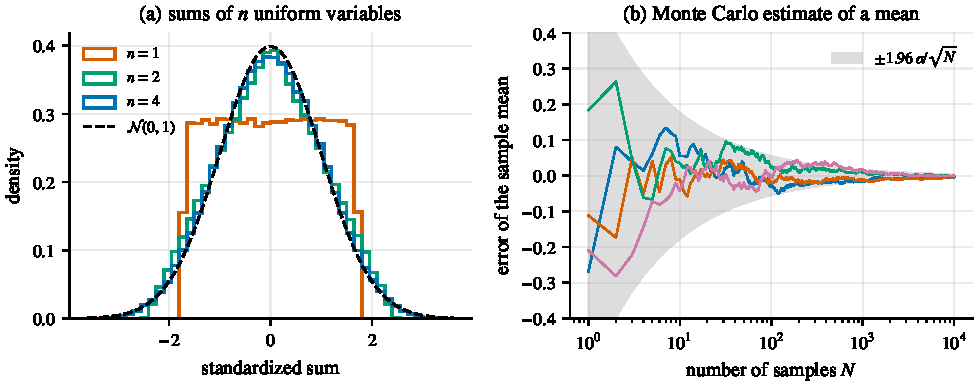
\includegraphics[width=\textwidth]{fig_clt.pdf}
  \caption{(a) The central limit theorem: histograms of the standardized sum of $n$ independent uniform variables approach the standard normal
  density already for $n = 4$. (b) Monte Carlo estimation of a mean: the error of the sample mean shrinks like $1/\sqrt N$ (gray band:
  $\pm1.96\,\sigma/\sqrt N$, the 95\% interval).}
  \label{fig:clt}
\end{figure}

Sums of many small independent effects are approximately Gaussian, whatever the distribution of each effect (\cref{fig:clt}). Electronic
sensor noise is the sum of many microscopic fluctuations, and integrating a noisy signal sums many samples; both are why Gaussian noise
models work well in navigation. They work less well for rare large errors (outliers), which is why estimators also need gating and robust
methods (\cref{ch:updates,ch:nlls}).

% ==============================================================================
\section{The chi-squared distribution}
\label{sec:chi2}

\begin{definition}
\index{chi-squared distribution}
If $s_1, \dots, s_k$ are independent standard normal variables, $\gamma = \sum_{i=1}^k s_i^2$ has the $\chi^2$ distribution with $k$ degrees of freedom,
written $\gamma \sim \chi^2_k$.
\end{definition}

\begin{proposition}[Properties of $\chi^2_k$]
$\E[\gamma] = k$ and $\Var(\gamma) = 2k$. Its density is
\begin{equation}
  p(\gamma) = \frac{\gamma^{k/2 - 1}e^{-\gamma/2}}{2^{k/2}\,\Gamma(k/2)}, \qquad \gamma > 0,
\end{equation}
where $\Gamma$ is the gamma function ($\Gamma(m) = (m - 1)!$ for integers, $\Gamma(\tfrac12) = \sqrt\pi$).
\end{proposition}
\begin{proof}[Proof of the moments and of the case $k = 1$]
For $s \sim \N(0, 1)$, $\E[s^2] = 1$ and $\E[s^4] = 3$ (integration by parts), so $\Var(s^2) = 2$; the moments of the sum follow by additivity
over independent terms. For $k = 1$, $\gamma = s^2$ takes the value $\gamma$ when $s = \pm\sqrt\gamma$, so
$p(\gamma) = 2\cdot\frac{1}{\sqrt{2\pi}}e^{-\gamma/2}\cdot\frac{\dd\sqrt\gamma}{\dd\gamma} = \frac{1}{\sqrt{2\pi\gamma}}e^{-\gamma/2}$, which is the formula with $k = 1$.
The general case follows by convolving densities (or by integrating the Gaussian density over spherical shells).
\end{proof}

\begin{theorem}[Mahalanobis distance of a Gaussian]
\label{thm:mahalanobis-chi2}
If $x \sim \N(\mu, \Sigma)$ in $\R^k$ with $\Sigma \succ 0$, then $(x-\mu)\T\Sigma\inv(x - \mu) \sim \chi^2_k$.
\end{theorem}
\begin{proof}
With $\Sigma = LL\T$, the whitened vector $s = L\inv(x - \mu)$ is $\N(0, I)$ by \cref{prop:affine}, and $(x - \mu)\T\Sigma\inv(x-\mu) = s\T s = \sum_is_i^2$.
\end{proof}

\begin{figure}[t]
  \centering
  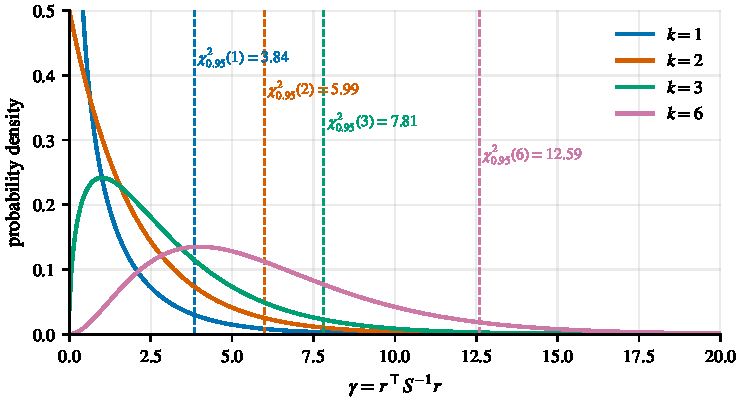
\includegraphics[width=0.84\textwidth]{fig_chi2.pdf}
  \caption{$\chi^2$ densities and their 95\% quantiles. A 2D image measurement whose normalized innovation squared exceeds $5.99$ would occur by
  chance only 5\% of the time if the filter's covariance were correct.}
  \label{fig:chi2}
\end{figure}

The \emph{quantile} $\chi^2_p(k)$ is the value below which a $\chi^2_k$ variable falls with probability $p$ (\cref{fig:chi2}; tables in
\cref{app:tables}). Because independent $\chi^2$ variables add, with their degrees of freedom adding, the sum of $N$ independent squared
Mahalanobis distances of $n$-dimensional Gaussians is $\chi^2_{Nn}$. As $k$ grows, $\chi^2_k$ is approximately $\N(k, 2k)$, so its quantiles approach
$k \pm 1.96\sqrt{2k}$.

% ==============================================================================
\section{Sample statistics and hypothesis tests}

\subsection{Estimating a mean and a variance}

Given independent samples $X_1, \dots, X_N$ of a distribution with unknown mean and variance, the natural estimates are the sample mean
$\bar X$ and the \term{sample variance}
\begin{equation}
  s^2 = \frac{1}{N - 1}\sum_{i=1}^N(X_i - \bar X)^2 .
\end{equation}
The divisor $N - 1$ makes $s^2$ unbiased. Expanding, $\sum_i(X_i - \bar X)^2 = \sum_i(X_i - \mu)^2 - N(\bar X - \mu)^2$, whose expectation is
$N\sigma^2 - N\cdot\sigma^2/N = (N - 1)\sigma^2$: one degree of freedom is used up by estimating the mean. For Gaussian samples one can show
moreover that $(N - 1)s^2/\sigma^2 \sim \chi^2_{N-1}$. This gives exact acceptance intervals for comparing a Monte Carlo sample variance with a
predicted variance, as Milestone 5 requires: the ratio $s^2/\sigma^2$ should lie between $\chi^2_{0.025}(N-1)/(N-1)$ and $\chi^2_{0.975}(N-1)/(N-1)$
95\% of the time (for $N = 500$, between $0.880$ and $1.128$; \cref{app:tables}).

\subsection{Hypothesis testing}

A \term{hypothesis test} decides whether data are compatible with a model. The recipe:
\begin{enumerate}
  \item State a \emph{null hypothesis} $H_0$, for example ``this measurement is consistent with the filter's prediction''.
  \item Choose a \emph{test statistic} whose distribution under $H_0$ is known, for example the squared Mahalanobis distance of the
        innovation, which is $\chi^2_m$ under $H_0$.
  \item Choose a \emph{significance level} $\alpha$ (often 5\%) and an \emph{acceptance region} that contains the statistic with probability
        $1 - \alpha$ under $H_0$.
  \item Reject $H_0$ if the statistic falls outside the region.
\end{enumerate}
Two errors are possible. A \emph{type I error} rejects a true $H_0$; by construction it happens with probability $\alpha$. A \emph{type II
error} accepts a false $H_0$; its probability depends on how different the truth is from $H_0$, and one minus it is the \emph{power} of the
test. Lowering $\alpha$ reduces false rejections at the price of more missed detections.

\emph{One-sided} tests reject only large values. Measurement gating is one-sided: a measurement is rejected when its Mahalanobis distance
exceeds $\chi^2_{1-\alpha}(m)$, because only large innovations indicate outliers (\cref{ch:updates}). \emph{Two-sided} tests reject both
unusually large and unusually small values. Filter consistency tests are two-sided: an average normalized error that is too small reveals an
underconfident filter just as one that is too large reveals an overconfident one (\cref{ch:consistency}).

\begin{pitfall}[a 5\% test rejects 5\% of good data]
At a 95\% gate, one in twenty perfectly good measurements is rejected. Over thousands of measurements this is expected and harmless,
provided rejections are counted. A rejection rate far from the design value is itself a symptom worth investigating.
\end{pitfall}

% ==============================================================================
\section{Nonlinear transformations}
\label{sec:linearization}

If $y = f(x)$ with $f$ nonlinear and $x \sim \N(\mu, \Sigma)$, then $y$ is generally \emph{not} Gaussian. The extended Kalman filter approximates it
by a Gaussian, linearizing $f$ about the mean:
\begin{equation}
  y \approx f(\mu) + J(x - \mu), \quad J = \frac{\partial f}{\partial x}\Big|_{\mu}
  \qquad\Longrightarrow\qquad
  y \mathrel{\dot\sim} \N\big(f(\mu),\ J\Sigma J\T\big).
\end{equation}
How much does this miss? In one dimension, Taylor expansion to second order gives
$f(x) \approx f(\mu) + f'(\mu)(x - \mu) + \tfrac12f''(\mu)(x - \mu)^2$, and taking expectations,
\begin{equation}
  \E[f(x)] \approx f(\mu) + \tfrac12f''(\mu)\,\sigma^2 .
\end{equation}
Linearization therefore ignores a \emph{bias} proportional to the curvature times the variance. The approximation is good when $f$ is nearly
linear over the region where $x$ has most of its probability mass, a few standard deviations around $\mu$.

\begin{figure}[t]
  \centering
  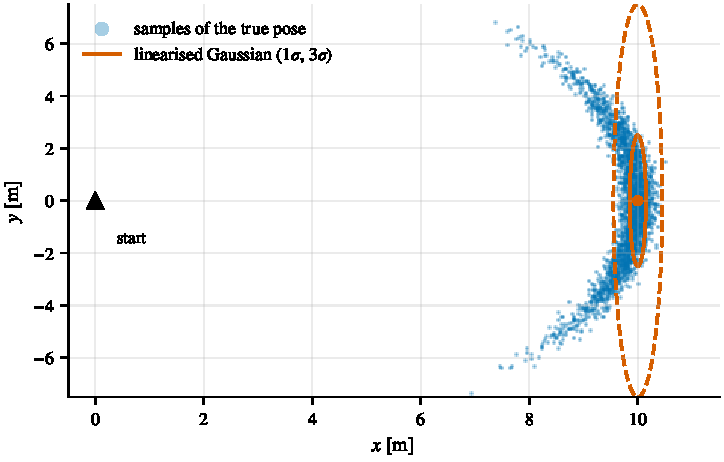
\includegraphics[width=0.84\textwidth]{fig_banana.pdf}
  \caption{A robot drives 10~m with a heading uncertainty of $\sigma_\psi = 0.25$~rad. The true distribution of its final position (samples) is a
  curved ``banana''. The linearized Gaussian (ellipses) matches its first two moments only locally, puts probability where the robot cannot be,
  and misses the curvature. Errors of this kind are why an estimator must keep its errors small, the central design principle of the
  error-state filter.}
  \label{fig:banana}
\end{figure}

\Cref{fig:banana} shows a classic failure. When heading uncertainty is large, positions are distributed along an arc, and the linearized Gaussian
is a poor description: its mean lies outside the arc, and it assigns probability to positions the robot cannot reach. Two remedies exist.
One is to reduce the uncertainty that must be linearized: the error-state filter of \cref{ch:eskf} keeps the estimation error, not the state,
as the quantity it linearizes, and continually resets it to zero. The other is to choose coordinates in which the distribution is close to
Gaussian: a Gaussian on the heading angle and travelled distance, pushed through the exact kinematics, reproduces the banana. \Cref{ch:lie}
develops that idea for rotations, and \cref{ch:nonlinear} presents a third remedy, sigma-point methods that propagate a few carefully chosen
samples instead of a linearization.

\begin{takeaways}
\begin{itemize}
  \item Bayes' rule converts a sensor model $p(z\mid x)$ and a prior $p(x)$ into the posterior $p(x\mid z)$.
  \item Affine maps propagate covariances as $A\Sigma A\T$. This single fact drives prediction, cloning and stacking.
  \item $\E[x\T Ax] = \tr(A\Sigma) + \mu\T A\mu$; the normalized squared error of an $n$-dimensional Gaussian averages to $n$.
  \item In covariance form, marginalization deletes rows and columns and conditioning takes a Schur complement. Information form is the reverse.
  \item Fusing independent Gaussian information adds inverse covariances; the result is a gain-weighted correction.
  \item Monte Carlo errors shrink like $1/\sqrt N$; sums of many small effects are nearly Gaussian.
  \item The squared Mahalanobis distance of an $n$-dimensional Gaussian is $\chi^2_n$: the basis of gating and consistency tests.
  \item Linearization ignores curvature-induced bias and fails when uncertainty is large relative to curvature.
\end{itemize}
\end{takeaways}

\begin{exercises}
  \item A gyro is either healthy (99\%) or faulty (1\%). A self-test flags 98\% of faulty units and 3\% of healthy ones. A unit is flagged; what is
        the probability that it is faulty?
  \item Let $x \sim \N(0, \diag(1, 4))$ and $y = Ax$ with $A$ a rotation by $30^\circ$. Compute $\Cov(y)$ and sketch the $1\sigma$ ellipses of $x$ and $y$.
  \item Prove that $\Sigma_{a|b} \preceq \Sigma_{aa}$: conditioning never increases uncertainty in the Loewner order. When is the inequality an equality?
  \item Derive the information-form marginal $\Lambda_{aa} - \Lambda_{ab}\Lambda_{bb}\inv\Lambda_{ba}$ from \cref{prop:block-inverse} and show that it equals $\Sigma_{aa}\inv$.
  \item Complete the square to derive \eqref{eq:fusion}.
  \item Solve \eqref{eq:map-ls} by setting the gradient to zero, and show that the solution can be written $\hat x = \mu + K(z - H\mu)$ for
        $K = (P\inv + H\T R\inv H)\inv H\T R\inv$.
  \item For $x \sim \N(0, \sigma^2)$ and $y = x^2$, compute the exact mean of $y$ and its first-order linearized prediction. Explain the discrepancy.
  \item What fraction of a 2D Gaussian's probability lies inside its $1\sigma$ Mahalanobis ellipse? (Hint: $P(\chi^2_2 \le 1)$.) Inside its $3\sigma$ ellipse?
  \item Show that $\E[s^4] = 3$ for $s \sim \N(0, 1)$ by integrating by parts.
  \item A Monte Carlo test with $N = 100$ runs finds a sample variance 25\% larger than predicted. Is this evidence of an error at the 5\% level?
\end{exercises}
\input{chapters/solutions/05_probability}

\chapter{Random Processes, Spectra and Sensor Noise}
\label{ch:processes}
\chaptermark{Random Processes and Noise} % short running header

\begin{objectives}
\begin{itemize}
  \item Describe noise that evolves in time: random sequences, autocorrelation, stationarity, white noise and random walks.
  \item Understand power spectral densities and why sensor noise is specified in units per $\sqrt{\mathrm{Hz}}$.
  \item Understand continuous-time white noise, its sampling, and aliasing.
  \item Derive how integrated noise grows, and how covariance evolves in a linear stochastic system.
  \item Derive the Allan variance signatures used to identify IMU noise parameters.
  \item Model colored noise with shaping filters, the reason sensor biases become filter states.
\end{itemize}
\end{objectives}

\Cref{ch:prob} dealt with random vectors: a fixed number of uncertain quantities. Sensor noise is a different kind of object: a random
\emph{signal}, a function of time, whose values at different times may or may not be related. This chapter develops the theory of such
random processes, as far as it is needed to understand IMU datasheets, to model sensor errors in a filter, and to discretize those models
correctly.

% ==============================================================================
\section{Random sequences}

\subsection{Definitions}

A \term{random sequence} (discrete-time random process) is a sequence of random variables $x_0, x_1, x_2, \dots$, for example the noise
added to successive IMU samples. One run of the experiment produces one \emph{sample path}; repeating the experiment produces another.
Statistics are taken across this \emph{ensemble} of paths. The \emph{mean function} is $\mu_k = \E[x_k]$ and the \emph{autocovariance}
\begin{equation}
  C(k, j) = \E\big[(x_k - \mu_k)(x_j - \mu_j)\big]
\end{equation}
says how strongly the values at two times are related. A sequence is \term{wide-sense stationary} if its mean is constant and its
autocovariance depends only on the lag, $C(k, j) = C(k - j)$: its statistical character does not change with time.

\subsection{Three fundamental sequences}

\begin{figure}[t]
  \centering
  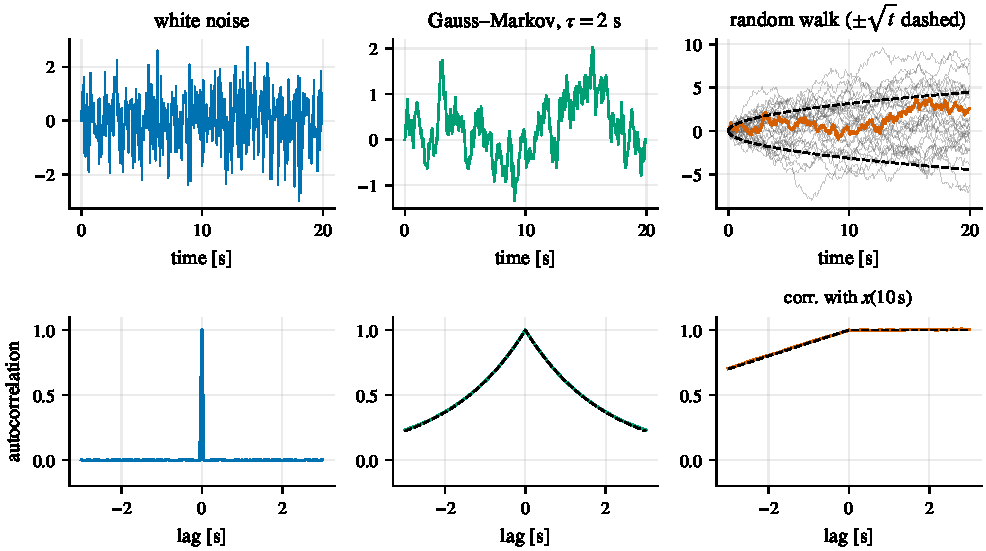
\includegraphics[width=\textwidth]{fig_processes.pdf}
  \caption{Sample paths (top) and autocorrelation functions (bottom) of white noise, a first-order Gauss--Markov sequence with correlation time
  $\tau = 2$~s, and a random walk, all driven by the same white sequence. White noise is uncorrelated with itself at any non-zero lag;
  the Gauss--Markov sequence forgets its past exponentially; the random walk never forgets and its spread grows like $\sqrt t$.}
  \label{fig:processes}
\end{figure}

\paragraph{White noise.} A \term{white sequence} has zero mean and uncorrelated values: $C(k) = \sigma^2$ for $k = 0$ and $0$ otherwise. Each
sample carries no information about the others. The measurement noise of a well-behaved sensor is approximately white.

\paragraph{Random walk.} Summing white noise gives a \term{random walk}: $x_{k+1} = x_k + w_k$, $x_0 = 0$, with $w_k$ white of variance $\sigma^2$. Then
$x_k = \sum_{j<k}w_j$ and, because variances of uncorrelated terms add,
\begin{equation}
  \Var(x_k) = k\sigma^2 .
\end{equation}
The spread grows like $\sqrt k$ without bound, and the sequence is not stationary. Its autocovariance $C(k, j) = \min(k, j)\sigma^2$ shows that
it remembers its whole past. Slowly drifting sensor biases are modeled as random walks.

\paragraph{First-order Gauss--Markov sequence.} Between the two lies $x_{k+1} = ax_k + w_k$ with $|a| < 1$. If the sequence is stationary, taking the
variance of both sides gives $V = a^2V + \sigma^2$, so
\begin{equation}
  \Var(x_k) = \frac{\sigma^2}{1 - a^2}, \qquad C(j) = \frac{\sigma^2}{1 - a^2}\,a^{|j|},
\end{equation}
the second because $x_{k+j} = a^jx_k + (\text{noise uncorrelated with } x_k)$. The sequence forgets its past exponentially, with a
\emph{correlation time} of about $1/(1 - a)$ steps. It is a bounded, slowly varying error: a useful model for biases that wander but do not
diverge, and for many environmental disturbances.

% ==============================================================================
\section{Frequency-domain description}

\subsection{Fourier analysis in brief}

Every reasonable signal is a superposition of sinusoids. The \term{Fourier transform}
\begin{equation}
  X(f) = \int_{-\infty}^{\infty}x(t)\,e^{-i2\pi ft}\,\dd t, \qquad x(t) = \int_{-\infty}^{\infty}X(f)\,e^{i2\pi ft}\,\dd f
\end{equation}
gives the complex amplitude $X(f)$ of the component at frequency $f$ (in Hz). Two facts are all we need. First, Parseval's theorem
$\int|x(t)|^2\dd t = \int|X(f)|^2\dd f$: energy can be counted in time or in frequency. Second, linear time-invariant systems (filters) act
on each frequency independently, multiplying $X(f)$ by a \emph{frequency response} $H(f)$. A low-pass filter has $|H(f)| \approx 1$ at low
frequencies and $|H(f)| \approx 0$ at high ones.

\subsection{Power spectral density}

A random signal has infinite energy (it goes on forever), but finite \emph{power}. Its \term{power spectral density} (PSD) describes how that
power is distributed over frequency.

\begin{definition}[Power spectral density]
For a wide-sense stationary process with autocovariance $C(\tau) = \E[x(t + \tau)x(t)]$ (zero mean), the (two-sided) PSD is
\begin{equation}
  S(f) = \int_{-\infty}^{\infty}C(\tau)\,e^{-i2\pi f\tau}\,\dd\tau .
\end{equation}
\end{definition}

This relation between the autocovariance and the PSD is the \emph{Wiener--Khinchin theorem}. Evaluating the inverse transform at $\tau = 0$ shows
that the variance is the total area under the PSD:
\begin{equation}
  \Var(x) = C(0) = \int_{-\infty}^\infty S(f)\,\dd f .
\end{equation}
So $S(f)\,\dd f$ is the contribution of the frequency band $[f, f + \dd f]$ to the variance, and the PSD has units of $[x]^2/\mathrm{Hz}$. Passing
the process through a filter with frequency response $H(f)$ multiplies its PSD by $|H(f)|^2$.

\begin{pitfall}[one-sided and two-sided PSDs]
Engineers often use a \emph{one-sided} PSD defined only for $f \ge 0$ and equal to twice the two-sided one, so that the variance is
$\int_0^\infty S_1(f)\,\dd f$. Datasheets rarely say which convention they use, and the two differ by a factor of $\sqrt2$ in the noise density.
These notes use the convention of the EuRoC calibration files and of most of the VIO literature: a continuous white noise $w$ with
$\E[w(t)w(s)] = \sigma^2\delta(t - s)$, i.e.\ two-sided PSD $\sigma^2$.
\end{pitfall}

% ==============================================================================
\section{Continuous-time white noise}
\label{sec:ct-noise}

\begin{definition}[Continuous-time white noise]
\index{white noise}
A zero-mean process $w(t) \in \R^n$ is white with \term{noise density} (intensity) $Q_c$ if
$\E[w(t)\,w(s)\T] = Q_c\,\delta(t - s)$, where $\delta$ is the Dirac delta. For a scalar process we write $Q_c = \sigma^2$ and call $\sigma$ the noise
density.
\end{definition}

Continuous white noise is an idealization: its PSD is flat at all frequencies, so its variance $\int S\,\dd f$ is infinite. Physical noise is
white only up to some bandwidth. What makes the idealization useful is that its \emph{integrals} are perfectly well behaved: the integral of
white noise over an interval of length $T$ is a zero-mean random variable with variance
\begin{equation}
  \Var\Big(\int_0^Tw(t)\,\dd t\Big) = \int_0^T\!\!\int_0^T\sigma^2\delta(t - s)\,\dd s\,\dd t = \sigma^2T .
\end{equation}
Since $\delta$ has units of 1/time, $\sigma$ has units of $[w]\cdot\sqrt{\mathrm s} = [w]/\sqrt{\mathrm{Hz}}$. For a gyroscope, $[w] = \mathrm{rad/s}$, so its
noise density is in $\mathrm{rad/s/\sqrt{Hz}}$, the units of \code{gyroscope\_noise\_density} in EuRoC's \code{sensor.yaml}.

\paragraph{From continuous to discrete noise.} A digital sensor reports samples every $\Dt$. If each sample is the average of the
continuous white input over its interval, which an anti-aliasing filter approximates, the sample noise has variance
\begin{equation}
  \Var\Big(\frac1\Dt\int_0^\Dt w(s)\,\dd s\Big) = \frac{\sigma^2}{\Dt}, \qquad \sigma_{\mathrm{discrete}} = \frac{\sigma}{\sqrt{\Dt}} .
  \label{eq:discrete-noise}
\end{equation}
The frequency-domain view agrees: an ideal low-pass filter that keeps the band $|f| < f_s/2$ (with $f_s = 1/\Dt$) passes a variance of
$\int_{-f_s/2}^{f_s/2}\sigma^2\,\dd f = \sigma^2f_s = \sigma^2/\Dt$. Sampling faster does not reduce the noise per unit time; it merely spreads it over
more samples, each noisier. For EuRoC's gyroscope, $\sigma_g = 1.6968\times10^{-4}~\mathrm{rad/s/\sqrt{Hz}}$ at 200~Hz gives a per-sample standard
deviation of $2.4\times10^{-3}$~rad/s.

Conversely, a random walk driven by white noise, $\dot b = w$, gains variance $\sigma^2\Dt$ over a step $\Dt$, so its exact discretization is
$b_{k+1} = b_k + \sqrt{\Dt}\,\sigma\,s_k$ with $s_k \sim \N(0, 1)$. The two conversions go in opposite directions, $\sigma/\sqrt\Dt$ for the sample noise
and $\sigma\sqrt\Dt$ for the walk; confusing them is a classic error in noise simulators.

% ==============================================================================
\section{Sampling and aliasing}

\begin{theorem}[Sampling theorem, Nyquist--Shannon]
\index{sampling theorem}
A signal containing no frequencies at or above $f_s/2$ is completely determined by its samples at rate $f_s$. The frequency $f_s/2$ is the
\term{Nyquist frequency}.
\end{theorem}

\begin{figure}[t]
  \centering
  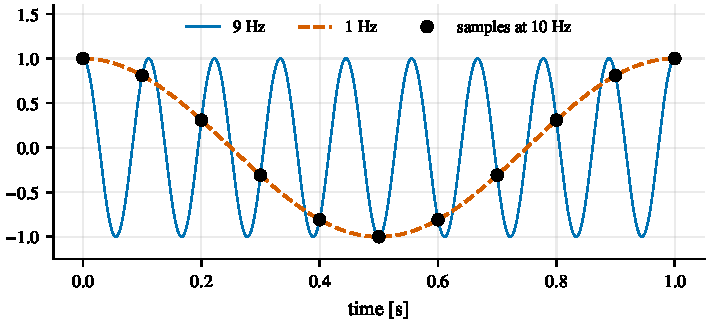
\includegraphics[width=0.9\textwidth]{fig_aliasing.pdf}
  \caption{Aliasing. A 9~Hz sinusoid sampled at 10~Hz (dots) produces exactly the same samples as a 1~Hz sinusoid (dashed). After sampling, the
  two are indistinguishable.}
  \label{fig:aliasing}
\end{figure}

A component at a frequency $f$ above the Nyquist frequency does not disappear when sampled: it masquerades as a lower frequency
$|f - kf_s|$ for the integer $k$ that brings it into $[0, f_s/2]$ (\cref{fig:aliasing}). This \term{aliasing} cannot be undone after sampling, so it
must be prevented before, by an analog or digital \emph{anti-aliasing} low-pass filter. IMUs contain such filters, but strong vibration near
or above the sampling rate (propellers at hundreds of Hz) can still alias into low frequencies and appear as bias-like errors. The same
principle governs images: a camera samples a scene spatially, and an image must be blurred before it is down-sampled, or fine textures turn
into false coarse patterns (\cref{ch:imageproc}).

% ==============================================================================
\section{Integrated noise}

\begin{proposition}[Integrated white noise]
\label{prop:integrated-noise}
Let $w$ be scalar white noise with density $\sigma$. The $m$-fold integral
$I_m(t) = \int_0^t \int_0^{t_1}\cdots\int_0^{t_{m-1}} w(t_m)\,\dd t_m \cdots \dd t_1$ has zero mean and
\begin{equation}
  \Var\big(I_m(t)\big) = \sigma^2\,\frac{t^{2m-1}}{(2m-1)\,\big((m-1)!\big)^2}.
  \label{eq:integrated-noise}
\end{equation}
For $m = 1, 2, 3, 4$ this gives $\sigma^2 t$, $\sigma^2 t^3/3$, $\sigma^2 t^5/20$ and $\sigma^2 t^7/252$.
\end{proposition}
\begin{proof}
By Cauchy's formula for repeated integration (proved by induction, exchanging the order of integration),
$I_m(t) = \int_0^t \frac{(t - s)^{m-1}}{(m-1)!}\,w(s)\,\dd s$. For a weighted integral $\int g(s)w(s)\,\dd s$ of white noise,
$\Var = \iint g(s)g(s')\,\sigma^2\delta(s - s')\,\dd s\,\dd s' = \sigma^2\int g(s)^2\,\dd s$. Here
$\int_0^t (t-s)^{2m-2}\,\dd s/((m-1)!)^2 = t^{2m-1}/((2m-1)((m-1)!)^2)$.
\end{proof}

The single integral $I_1$ is the continuous random walk, or \term{Wiener process}, whose standard deviation grows like $\sqrt t$. Integrating
accelerometer white noise twice into position gives $\sigma_a^2t^3/3$: position uncertainty grows like $t^{3/2}$. Each further integration adds
two powers of $t$ to the variance. \Cref{ch:errordyn} uses this proposition to explain how fast an inertial navigator degrades.

% ==============================================================================
\section{Linear stochastic differential equations}
\label{sec:lyapunov}

Most noise models in navigation are linear systems driven by white noise:
\begin{equation}
  \dot x(t) = F(t)\,x(t) + G(t)\,w(t), \qquad \E[w(t)w(s)\T] = Q_c\,\delta(t - s).
  \label{eq:linear-sde}
\end{equation}
Because white noise is so irregular, such equations are made rigorous by stochastic calculus. For linear systems, however, the results we
need follow from a simple limiting argument.

\begin{proposition}[Mean and covariance propagation]
\label{prop:lyapunov}
\index{Lyapunov equation}
For \eqref{eq:linear-sde}, the mean $m(t) = \E[x(t)]$ and covariance $P(t)$ evolve as
\begin{equation}
  \dot m = Fm, \qquad \dot P = FP + PF\T + GQ_cG\T,
  \label{eq:lyapunov-ode}
\end{equation}
with solution $P(t) = \Phi(t, t_0)P(t_0)\Phi(t, t_0)\T + \int_{t_0}^t\Phi(t, s)G(s)Q_cG(s)\T\Phi(t, s)\T\,\dd s$.
\end{proposition}
\begin{proof}
Over a short interval $h$, $x(t + h) = (I + Fh)x(t) + \int_t^{t+h}Gw\,\dd s + O(h^2)$, and the noise integral is zero-mean with covariance $GQ_cG\T h$ and
uncorrelated with $x(t)$. By \cref{prop:affine}, $P(t + h) = (I + Fh)P(I + Fh)\T + GQ_cG\T h + O(h^2) = P + (FP + PF\T + GQ_cG\T)h + O(h^2)$. Subtract
$P(t)$, divide by $h$ and let $h\to0$. The integral form is verified by differentiating it (\cref{prop:stm}).
\end{proof}

\Cref{eq:lyapunov-ode} is the \emph{Lyapunov differential equation}. The first two terms move and shape the existing uncertainty with the
dynamics; the last term pumps in new uncertainty from the noise. Its integral form over one time step is exactly the discrete process noise
covariance $Q_d$ of the Kalman filter (\cref{ch:linsys,ch:kf}). For a stable time-invariant system, $P$ approaches the solution of the
algebraic Lyapunov equation $0 = FP + PF\T + GQ_cG\T$.

\subsection{The continuous Gauss--Markov process}

The scalar system $\dot x = -x/\tau + w$ with noise density $\sigma$ is the continuous counterpart of the Gauss--Markov sequence. Its stationary
variance solves $0 = -2P/\tau + \sigma^2$:
\begin{equation}
  P_\infty = \frac{\sigma^2\tau}{2}, \qquad C(\Delta t) = P_\infty\,e^{-|\Delta t|/\tau}, \qquad S(f) = \frac{\sigma^2\tau^2}{1 + (2\pi f\tau)^2} .
\end{equation}
(The PSD is the white input PSD $\sigma^2$ times $|H(f)|^2$ for the system's frequency response $H(f) = 1/(i2\pi f + 1/\tau)$; integrating it over all
frequencies returns $P_\infty$.) The autocovariance decays with time constant $\tau$, and the PSD is flat up to the corner frequency $1/(2\pi\tau)$ and
falls off beyond it. Its exact discretization over $\Dt$ is $x_{k+1} = e^{-\Dt/\tau}x_k + w_k$ with $\Var(w_k) = P_\infty(1 - e^{-2\Dt/\tau})$. As
$\tau\to\infty$ it becomes a random walk; as $\tau\to0$ with the low-frequency level $\sigma^2\tau^2$ of its PSD held fixed, it becomes white noise.

% ==============================================================================
\section{Colored noise and state augmentation}

A Kalman filter assumes that its process and measurement noises are white. When a disturbance is \emph{colored} (correlated in time), the
standard remedy is to model it as the output of a linear system driven by white noise, a \emph{shaping filter}, and to add the state of that
system to the filter state. A sensor bias that drifts as a random walk is exactly this: $b$ is colored, but $\dot b = w_b$ is white-driven, so
$b$ becomes part of the state. This is why IMU biases appear in the state vector of every inertial filter (\cref{ch:imu}). Ignoring the
correlation, and treating a slowly varying error as white, makes the filter believe that errors average out when they do not, and leads to
overconfidence.

% ==============================================================================
\section{The Allan variance}
\label{sec:allan}

How are the noise densities of a sensor measured? Record it at rest for hours and compute its \term{Allan variance}, a tool developed for
characterizing atomic clocks that separates noise processes by their time scale.

\begin{definition}[Allan variance]
Split a record of rate samples $y(t)$ into consecutive clusters of duration $\tau$, and let $\bar y_k(\tau)$ be the average over cluster $k$. The
Allan variance is half the mean squared difference of consecutive cluster averages:
\begin{equation}
  \sigma_A^2(\tau) = \tfrac12\,\E\big[(\bar y_{k+1}(\tau) - \bar y_k(\tau))^2\big] .
\end{equation}
\end{definition}

In practice it is computed from the integrated signal $\theta(t) = \int_0^ty$ (for a gyroscope, the angle), since
$\bar y_{k+1} - \bar y_k = (\theta_{k+2} - 2\theta_{k+1} + \theta_k)/\tau$ with $\theta_j = \theta(j\tau)$. The \emph{overlapping} estimator averages over all
starting times rather than only disjoint clusters, which uses the data more efficiently.

\begin{proposition}[Allan variance signatures]
For white noise of density $\sigma$, $\sigma_A^2(\tau) = \sigma^2/\tau$. For a random walk $\dot b = w_b$ with density $\sigma_b$, $\sigma_A^2(\tau) = \sigma_b^2\tau/3$.
\end{proposition}
\begin{proof}
\emph{White noise.} Each cluster average is an integral of white noise divided by $\tau$, with variance $\sigma^2\tau/\tau^2 = \sigma^2/\tau$; consecutive
averages involve disjoint intervals and are uncorrelated, so their difference has variance $2\sigma^2/\tau$, and half of it is $\sigma^2/\tau$.
\emph{Random walk.} Write $b(t) = \int_0^tw_b$. The difference of two consecutive cluster averages is
$D = \frac1\tau\int_\tau^{2\tau}b\,\dd t - \frac1\tau\int_0^\tau b\,\dd t$. Substituting $b$ and exchanging the order of integration expresses $D$ as
$\frac1\tau\int_0^{2\tau}h(s)w_b(s)\,\dd s$ with $h(s) = s$ for $s \le \tau$ and $h(s) = 2\tau - s$ for $s > \tau$ (a triangular weight). Its variance is
$\frac{\sigma_b^2}{\tau^2}\big(\int_0^\tau s^2\dd s + \int_\tau^{2\tau}(2\tau - s)^2\dd s\big) = \frac{2}{3}\sigma_b^2\tau$, and half of it is $\sigma_b^2\tau/3$.
\end{proof}

On a log-log plot of the \emph{Allan deviation} $\sigma_A(\tau)$, independent noise processes therefore appear as straight lines with
characteristic slopes:
\begin{center}\small
\begin{tabular}{@{}l l l@{}}
\toprule
Process & $\sigma_A^2(\tau)$ & slope of $\sigma_A$ \\
\midrule
quantization noise & $3Q^2/\tau^2$ & $-1$ \\
white noise (density $\sigma$) & $\sigma^2/\tau$ & $-\tfrac12$ \\
bias instability ($B$) & $\approx (0.664 B)^2$ & $0$ \\
bias random walk (density $\sigma_b$) & $\sigma_b^2\tau/3$ & $+\tfrac12$ \\
rate ramp ($R$) & $R^2\tau^2/2$ & $+1$ \\
\bottomrule
\end{tabular}
\end{center}
The white-noise density is read off the $-\tfrac12$ line at $\tau = 1$~s, and the random-walk density off the $+\tfrac12$ line at $\tau = 3$~s. The
minimum of the curve marks the averaging time beyond which a stationary sensor's bias starts to wander; its height is related to the
\emph{bias instability}, a flicker-noise floor that neither white noise nor a random walk describes exactly.

\begin{figure}[t]
  \centering
  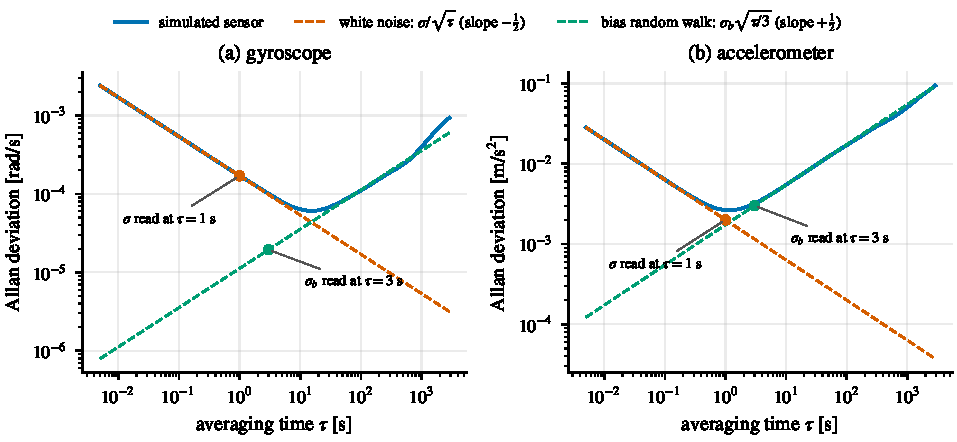
\includegraphics[width=\textwidth]{fig_allan.pdf}
  \caption{Allan deviation of a simulated 4-hour static recording with EuRoC's IMU noise parameters. The $-\tfrac12$ slope of white noise
  dominates short averaging times and the $+\tfrac12$ slope of the bias random walk dominates long ones. Reading the asymptotes at
  $\tau = 1$~s and $\tau = 3$~s recovers the densities.}
  \label{fig:allan}
\end{figure}

\Cref{fig:allan} shows the procedure on simulated data with the EuRoC parameters of \cref{ch:imu}. On real sensors, a flat bias-instability
region appears near the minimum, which the random-walk model only approximates. The IEEE standard procedure~\cite{ieee952} and El-Sheimy et
al.~\cite{elsheimy2008allan} give practical details.

\begin{takeaways}
\begin{itemize}
  \item White noise is uncorrelated in time; a random walk is its running sum, with variance growing linearly; a Gauss--Markov process
        forgets its past exponentially.
  \item The PSD distributes a process's variance over frequency; noise densities are square roots of PSDs, in units per $\sqrt{\mathrm{Hz}}$.
  \item Sampling white noise of density $\sigma$ at period $\Dt$ gives per-sample noise $\sigma/\sqrt\Dt$; a random walk gains $\sigma_b\sqrt\Dt$ per step.
  \item Frequencies above Nyquist alias; filter before you sample or down-sample.
  \item The $m$-fold integral of white noise has variance growing like $t^{2m-1}$.
  \item Covariance in a linear stochastic system obeys $\dot P = FP + PF\T + GQ_cG\T$.
  \item Colored noise is modeled with a shaping filter whose state joins the filter state: this is why biases are states.
  \item The Allan deviation separates white noise (slope $-\tfrac12$, read at 1~s) from bias random walk (slope $+\tfrac12$, read at 3~s).
\end{itemize}
\end{takeaways}

\begin{exercises}
  \item Show that the autocovariance of a random walk is $C(k, j) = \min(k, j)\,\sigma^2$.
  \item For the Gauss--Markov sequence with $a = 0.99$ and $\sigma = 1$, compute the stationary standard deviation and the lag at which the
        correlation drops below $1/e$.
  \item A 1~kHz accelerometer has white noise of $2\times10^{-3}~\mathrm{m/s^2/\sqrt{Hz}}$. What is the standard deviation of a single sample? Of the average
        of 1000 consecutive samples? Of a single sample of the same sensor read at 100~Hz?
  \item A 105~Hz vibration is sampled at 100~Hz. At what frequency does it appear?
  \item Verify \cref{prop:integrated-noise} by Monte Carlo for $m = 2$ and $m = 3$, simulating at 200~Hz for 10~s with 1000 runs.
  \item Solve the Lyapunov equation for the double integrator $\dot p = v$, $\dot v = w$ with $P(0) = 0$ and verify that $P_{pp}(t) = \sigma^2t^3/3$.
  \item Derive the stationary variance and the exact discretization of the continuous Gauss--Markov process.
  \item Simulate 2 hours of a gyro with EuRoC parameters, compute the overlapping Allan deviation, and recover $\sigma_g$ and $\sigma_{b_g}$ from the
        asymptotes. How long a recording is needed to estimate $\sigma_{b_g}$ to 10\%?
\end{exercises}

\chapter{Rotations, Quaternions and Rigid-Body Kinematics}
\label{ch:rotations}
\chaptermark{Rotations and Quaternions} % short running header

\begin{objectives}
\begin{itemize}
  \item Read and write frame-annotated transformations such as $R_{wb}$, $p_{wb}$ and $T_{bc}$ without ambiguity, and catch frame bugs
        with the adjacency rule.
  \item Understand rotations in the plane, then in space: rotation matrices, axis-angle and Rodrigues' formula.
  \item Understand Euler angles, intrinsic versus extrinsic sequences, their conversions, and why they are banned from the estimator.
  \item Derive Hamilton quaternion algebra and its rotation formula; convert between quaternions and matrices; interpolate; and
        translate formulas from the JPL convention.
  \item Derive the kinematics of rotating bodies: $\dot R = R\sx{\omega}$, $\dot q = \tfrac12 q\qprod[0,\omega]$, the transport theorem and the Coriolis
        acceleration, and quantify the effects of the Earth's rotation.
\end{itemize}
\end{objectives}

% ==============================================================================
\section{Frames and notation}

A \term{frame} is an origin together with three orthonormal, right-handed axes. Three frames appear in this project (\cref{fig:frames}).

\begin{convention}[frames, AGENTS.md C1]
\begin{itemize}
  \item $W$, the \textbf{world} frame: fixed, gravity-aligned with $z$ pointing up, the frame of the ground truth (EuRoC calls it
        \code{R}). Gravity is $g_w = [0, 0, -9.81]\T~\mathrm{m/s^2}$.
  \item $B$, the \textbf{body} frame: the IMU frame \code{imu0} (EuRoC's \code{S} in \code{imu0}).
  \item $C$, the left \textbf{camera} frame \code{cam0}: origin at the optical center, $z$ along the optical axis, $x$ to the right and $y$
        down in the image.
\end{itemize}
$R_{wb}$ (or $q_{wb}$) maps body-frame coordinates to world-frame coordinates, $v_w = R_{wb}v_b$. $p_{wb}$ is the position of the origin of $B$
expressed in $W$. $v_{wb}$ is the velocity of $B$ relative to $W$, expressed in $W$. $T_{bc} = (R_{bc}, p_{bc})$ maps camera points into the body
frame, $p_b = R_{bc}p_c + p_{bc}$; it is \code{T\_BS} from \code{cam0/sensor.yaml}. A world-to-body rotation is never used as a state.
\end{convention}

\begin{figure}[t]
\centering
\begin{tikzpicture}[scale=1.0]
  \coordinate (W) at (0,0);
  \draw[frameaxis, plotorange] (W) -- ++(1.4,0) node[right] {$x_w$};
  \draw[frameaxis, plotgreen] (W) -- ++(0.75,0.6) node[above right] {$y_w$};
  \draw[frameaxis, plotblue] (W) -- ++(0,1.4) node[above] {$z_w$};
  \node[below left] at (W) {$W$};
  \draw[->, thick, black!60] (-0.6,1.0) -- ++(0,-0.8) node[midway, left] {$g$};
  \coordinate (B) at (5.2,2.2);
  \begin{scope}[shift={(B)}, rotate=25]
    \draw[fill=primarylight, draw=primary, rounded corners=2pt] (-0.55,-0.25) rectangle (0.55,0.25);
    \draw[frameaxis, plotorange] (0,0) -- (1.3,0) node[right] {$x_b$};
    \draw[frameaxis, plotgreen] (0,0) -- (0.65,0.55) node[above right] {$y_b$};
    \draw[frameaxis, plotblue] (0,0) -- (0,1.3) node[above] {$z_b$};
    \node[below left] at (-0.2,-0.25) {$B$ (IMU)};
    \coordinate (C) at (2.0,-1.3);
    \draw[fill=white, draw=primary] ($(C)+(-0.15,0.15)$) rectangle ($(C)+(0.15,-0.15)$);
    \draw[frameaxis, plotblue] (C) -- ++(0,-0.9) node[below] {$z_c$};
    \draw[frameaxis, plotorange] (C) -- ++(0.8,0) node[right] {$x_c$};
    \draw[frameaxis, plotgreen] (C) -- ++(-0.45,-0.35) node[left] {$y_c$};
    \node[above right] at ($(C)+(0.1,0.1)$) {$C$};
    \draw[->, thick, conv] (0.3,-0.3) to[bend right=20] node[midway, below left=-1pt] {$T_{bc}$} ($(C)+(-0.2,0.05)$);
  \end{scope}
  \draw[->, thick, primary, dashed] (W) -- (B) node[midway, above left] {$p_{wb}$, $R_{wb}$};
\end{tikzpicture}
\caption{The world frame $W$ (gravity-aligned, $z$ up), the body/IMU frame $B$ moving with the vehicle, and the camera frame $C$ rigidly
attached to the body through the constant extrinsic calibration $T_{bc}$.}
\label{fig:frames}
\end{figure}

\subsection{Reading subscripts}

The naming rule \code{<quantity>\_<to><from>} makes products self-checking. $R_{wb}$ takes a vector \emph{from} $B$ \emph{to} $W$. Composition
chains frames like dominoes:
\begin{equation}
  R_{wc} = R_{wb}\,R_{bc}, \qquad v_w = R_{wb}\,R_{bc}\,v_c .
\end{equation}

\begin{keyidea}[the adjacency rule]
\index{adjacency rule}
In a valid product, adjacent subscripts match: $R_{w\underline{b}}\,R_{\underline{b}c}$. A product such as $R_{wb}R_{cb}$ has mismatched neighbors and is
a bug. The fix is a transpose, $R_{wb}R_{cb}\T = R_{wb}R_{bc}$, since $R_{bc} = R_{cb}\inv = R_{cb}\T$. Apply the rule to every line of code that
multiplies rotations or transforms points.
\end{keyidea}

\subsection{Active and passive views}

A rotation matrix can be read in two ways. In the \emph{passive} view, $R_{wb}$ re-expresses the same physical vector in another frame:
$v_w$ and $v_b$ are coordinates of one arrow (\cref{sec:orthogonal-matrices}). In the \emph{active} view, $R_{wb}$ rotates the world axes
onto the body axes: its columns are the body axes $x_b, y_b, z_b$ expressed in world coordinates. Both readings describe the same matrix:
\begin{equation}
  R_{wb} = \begin{bmatrix} x_b^{(w)} & y_b^{(w)} & z_b^{(w)} \end{bmatrix}.
\end{equation}
This gives a quick sanity check when debugging: the third column of $R_{wb}$ is the body $z$-axis in world coordinates. For a level
vehicle whose $z$-axis points up, it is $[0,0,1]\T$; its third row is the world vertical expressed in the body frame.

% ==============================================================================
\section{Rotations in the plane}

Planar rotations contain most of the ideas of this chapter in their simplest form. The rotation by $\theta$ is (\cref{ex:rot2d})
\begin{equation}
  R(\theta) = \begin{bmatrix} \cos\theta & -\sin\theta \\ \sin\theta & \cos\theta \end{bmatrix}.
\end{equation}
Rotations compose by adding angles, $R(\alpha)R(\beta) = R(\alpha + \beta)$ (multiply out and use the angle-addition formulas), so planar
rotations commute. The angle is a perfect coordinate: $R(\theta)$ is determined by $\theta$, and every planar rotation is $R(\theta)$ for a
$\theta$ that is unique up to multiples of $2\pi$. The only subtlety is wrap-around: angles must be compared modulo $2\pi$, which is why the
difference between two headings is computed as $\atantwo(\sin(\theta_2 - \theta_1), \cos(\theta_2 - \theta_1))$ rather than $\theta_2 - \theta_1$.

Identifying the plane with the complex numbers, rotation by $\theta$ is multiplication by $e^{i\theta} = \cos\theta + i\sin\theta$. Unit complex
numbers compose by multiplication, and their angles add. Quaternions (\cref{sec:quaternions}) are the three-dimensional generalization of
this idea, with one crucial difference: in three dimensions, rotations do not commute.

% ==============================================================================
\section{Rotation matrices and \texorpdfstring{$\SO$}{SO(3)}}

\begin{definition}[Special orthogonal group]
\index{special orthogonal group}
$\SO = \{ R \in \R^{3\times3} : R\T R = I,\ \det R = +1 \}$.
\end{definition}

Orthogonality ($R\T R = I$) means $R$ preserves lengths and angles; $\det R = +1$ excludes reflections, which would turn a right-handed
frame into a left-handed one (\cref{sec:orthogonal-matrices}). The set is closed under multiplication and inversion, $R\inv = R\T$, so it is
a \emph{group}. A rotation matrix has nine entries but only three degrees of freedom: orthonormality imposes six constraints (three unit
lengths, three orthogonalities). This redundancy is why $\SO$ is a curved three-dimensional surface inside the nine-dimensional space of
matrices rather than a vector space; the sum of two rotation matrices is not a rotation matrix.

The elementary rotations about the coordinate axes follow from the planar case:
\begin{equation}
  R_x(\alpha) = \begin{bmatrix} 1 & 0 & 0 \\ 0 & c_\alpha & -s_\alpha \\ 0 & s_\alpha & c_\alpha \end{bmatrix},\quad
  R_y(\alpha) = \begin{bmatrix} c_\alpha & 0 & s_\alpha \\ 0 & 1 & 0 \\ -s_\alpha & 0 & c_\alpha \end{bmatrix},\quad
  R_z(\alpha) = \begin{bmatrix} c_\alpha & -s_\alpha & 0 \\ s_\alpha & c_\alpha & 0 \\ 0 & 0 & 1 \end{bmatrix},
\end{equation}
with $c_\alpha = \cos\alpha$, $s_\alpha = \sin\alpha$. (The signs of $R_y$ look reversed but are not: in the $z$-$x$ plane, ordered cyclically
after $y$, it is the usual planar rotation.) Rotations in space do not commute: $R_x(90^\circ)R_y(90^\circ) \ne R_y(90^\circ)R_x(90^\circ)$. Try it
with a book.

\section{Axis-angle and Rodrigues' formula}

By Euler's theorem (\cref{thm:euler-axis}), every rotation is a rotation by some angle $\theta \in [0, \pi]$ about some unit axis $u$. The pair
$(u, \theta)$ is the \term{axis-angle} representation, and $\phi = \theta u \in \R^3$ is the \term{rotation vector}: its direction is the axis and its
length the angle. The rotation vector is the central object of \cref{ch:lie}.

\begin{theorem}[Rodrigues' rotation formula]
\label{thm:rodrigues}
\index{Rodrigues' formula}
The rotation by angle $\theta$ about the unit axis $u$ is
\begin{equation}
  R = I + \sin\theta\,\sx{u} + (1 - \cos\theta)\,\sx{u}^2
    = \cos\theta\, I + (1-\cos\theta)\,u u\T + \sin\theta\,\sx{u}.
  \label{eq:rodrigues}
\end{equation}
\end{theorem}
\begin{proof}[Geometric proof]
Split any vector into components parallel and perpendicular to the axis (\cref{prop:projection-line}), $v = v_\parallel + v_\perp$ with
$v_\parallel = u u\T v$. Rotation leaves $v_\parallel$ unchanged and rotates $v_\perp$ by $\theta$ within the plane spanned by $v_\perp$ and
$u \times v_\perp = u \times v$ (a vector of the same length, rotated $90^\circ$ about $u$):
\begin{equation*}
  Rv = v_\parallel + \cos\theta\, v_\perp + \sin\theta\, u \times v .
\end{equation*}
Substituting $v_\perp = v - uu\T v = -\sx{u}^2 v$ (from \eqref{eq:skew-sq} with $\|u\|=1$) and $u \times v = \sx{u}v$ gives
$Rv = (I + \sin\theta\sx{u} + (1 - \cos\theta)\sx{u}^2)v$.
\end{proof}
\begin{proof}[Algebraic proof]
The rotation about $u$ at unit angular rate satisfies $\dot R = \sx{u} R$ (\cref{sec:rot-kinematics}), so $R(\theta) = \exp(\theta\sx{u})$ by
\cref{thm:lti-solution}. With $\sx{u}^3 = -\sx{u}$ from \eqref{eq:skew-cube}, all odd powers of $\sx{u}$ are $\pm\sx{u}$ and all even powers
(except the zeroth) are $\pm\sx{u}^2$, so the exponential series regroups as
\begin{equation*}
  \exp(\theta\sx{u}) = I + \Big(\theta - \tfrac{\theta^3}{3!} + \tfrac{\theta^5}{5!} - \cdots\Big)\sx{u}
     + \Big(\tfrac{\theta^2}{2!} - \tfrac{\theta^4}{4!} + \cdots\Big)\sx{u}^2,
\end{equation*}
and the two series are $\sin\theta$ and $1 - \cos\theta$.
\end{proof}

Two consequences of \eqref{eq:rodrigues} recover $(u, \theta)$ from $R$. Taking the trace (using $\tr\sx{u} = 0$ and $\tr\sx{u}^2 = -2$) and the
skew-symmetric part,
\begin{equation}
  \tr R = 1 + 2\cos\theta, \qquad R - R\T = 2\sin\theta\,\sx{u}.
  \label{eq:trace-angle}
\end{equation}
\Cref{ch:lie} shows that \emph{how} these are combined numerically matters a great deal.

\begin{worked}[a quarter turn]
Rotate by $\theta = 90^\circ$ about $u = e_z$: $\sx{e_z} = \begin{bmatrix}0 & -1 & 0\\1 & 0 & 0\\0 & 0 & 0\end{bmatrix}$ and
$\sx{e_z}^2 = \diag(-1, -1, 0)$, so \eqref{eq:rodrigues} gives $R = \begin{bmatrix}0 & -1 & 0\\ 1 & 0 & 0\\ 0 & 0 & 1\end{bmatrix} = R_z(90^\circ)$, which
sends $e_x$ to $e_y$, as a counter-clockwise quarter turn about $z$ should. Its trace is $1 = 1 + 2\cos90^\circ$.
\end{worked}

% ==============================================================================
\section{Euler angles}

\subsection{Definition and the two readings}

\term{Euler angles} describe a rotation as three successive rotations about coordinate axes. The aerospace yaw-pitch-roll ($ZYX$)
convention writes
\begin{equation}
  R_{wb} = R_z(\psi)\,R_y(\vartheta)\,R_x(\varphi),
  \label{eq:zyx}
\end{equation}
with yaw $\psi$, pitch $\vartheta$ and roll $\varphi$. The same product can be read in two ways, which are a constant source of confusion:
\begin{itemize}
  \item \emph{Intrinsic} (rotating axes): start aligned with the world, yaw by $\psi$ about $z$, then pitch by $\vartheta$ about the \emph{new} $y$-axis,
        then roll by $\varphi$ about the \emph{newest} $x$-axis. This is how a pilot thinks.
  \item \emph{Extrinsic} (fixed axes): roll by $\varphi$ about the world $x$-axis, then pitch by $\vartheta$ about the world $y$-axis, then yaw by $\psi$ about
        the world $z$-axis.
\end{itemize}
Both readings produce the same matrix \eqref{eq:zyx}; the intrinsic sequence $z, y', x''$ equals the extrinsic sequence $x, y, z$ in reverse
order. Twelve different axis sequences are in use, and each library documents its own. Always check the convention against a known example
before trusting a conversion.

\subsection{Conversions}

Multiplying out \eqref{eq:zyx} gives the third row of $R$ as $(-\sin\vartheta,\ \cos\vartheta\sin\varphi,\ \cos\vartheta\cos\varphi)$ and the first column as
$\cos\vartheta(\cos\psi, \sin\psi, \cdot)$. Hence
\begin{equation}
  \vartheta = \atantwo\big(-R_{31},\ \sqrt{R_{11}^2 + R_{21}^2}\big), \qquad
  \varphi = \atantwo(R_{32},\ R_{33}), \qquad
  \psi = \atantwo(R_{21},\ R_{11}) .
\end{equation}
When $\cos\vartheta = 0$ ($\vartheta = \pm90^\circ$), the formulas for $\varphi$ and $\psi$ become $\atantwo(0, 0)$: only their sum or difference is determined.

\subsection{Gimbal lock}

The relation between the body angular velocity measured by a gyroscope and the rates of the Euler angles is
\begin{equation}
  \begin{bmatrix} \dot\varphi \\ \dot\vartheta \\ \dot\psi \end{bmatrix}
  = \begin{bmatrix}
      1 & \sin\varphi\tan\vartheta & \cos\varphi\tan\vartheta \\
      0 & \cos\varphi & -\sin\varphi \\
      0 & \sin\varphi/\cos\vartheta & \cos\varphi/\cos\vartheta
    \end{bmatrix} \omega_b ,
  \label{eq:euler-rates}
\end{equation}
obtained by differentiating \eqref{eq:zyx} and comparing with $\sx{\omega_b} = R\T\dot R$ (\cref{sec:rot-kinematics}). At $\vartheta = \pm90^\circ$ the
matrix blows up. Geometrically, when the nose points straight up, yaw and roll rotate about the same physical axis, so the three angles no
longer describe three independent motions. This is \term{gimbal lock}, named after mechanical gimbal platforms that physically jam in this
configuration. Near the singularity, small angular velocities produce enormous Euler-angle rates, and a filter that linearizes in Euler
angles becomes numerically meaningless.

\begin{convention}[AGENTS.md C2]
Euler angles never appear in the estimator. They may appear only in telemetry and plots.
\end{convention}

No three-parameter representation of $\SO$ is free of singularities everywhere: a topological fact (the space $\SO$ cannot be covered by a
single chart). The solution adopted by modern estimators is to store attitude in a singularity-free \emph{redundant} representation (a unit
quaternion or a rotation matrix) and to use three parameters only for \emph{small} deviations around the current estimate, where no
singularity is near. That is the content of \cref{ch:lie}.

% ==============================================================================
\section{Quaternions}
\label{sec:quaternions}

\subsection{Quaternion algebra}

\index{quaternion}
A \term{quaternion} is a four-component number $q = w + x\,i + y\,j + z\,k$, written as a scalar part and a vector part, $q = [w,\ v]$ with
$v = (x,y,z)\T$. Hamilton's multiplication rules for the three imaginary units are
\begin{equation}
  i^2 = j^2 = k^2 = ijk = -1,
\end{equation}
from which $ij = k = -ji$, $jk = i = -kj$ and $ki = j = -ik$. (For example, multiplying $ijk = -1$ on the right by $k$ gives $ij(-1) = -k$.)
Expanding the product of two quaternions term by term with these rules and collecting the scalar and vector parts gives
\begin{equation}
  p \qprod q = \begin{bmatrix} p_w q_w - p_v\T q_v \\ p_w q_v + q_w p_v + p_v \times q_v \end{bmatrix}.
  \label{eq:qprod}
\end{equation}
The products of imaginary units produce exactly the components of the cross product, which makes the product non-commutative:
$p\qprod q - q\qprod p = [0,\ 2p_v\times q_v]$. It is associative. Because it is linear in each factor, it can be written with matrices,
\begin{equation}
  p\qprod q = [p]_L\, q = [q]_R\, p, \qquad
  [p]_L = \begin{bmatrix} p_w & -p_v\T \\ p_v & p_w I + \sx{p_v} \end{bmatrix}, \quad
  [q]_R = \begin{bmatrix} q_w & -q_v\T \\ q_v & q_w I - \sx{q_v} \end{bmatrix},
\end{equation}
where quaternions are treated as 4-vectors $[q_w;\ q_v]$.

The \emph{conjugate} is $q^* = [w,\ -v]$ and the \emph{norm} is $\|q\| = \sqrt{w^2 + \|v\|^2}$. By \eqref{eq:qprod}, $q\qprod q^* = [\|q\|^2,\ 0]$, so the
inverse is $q\inv = q^*/\|q\|^2$. Conjugation reverses products, $(p\qprod q)^* = q^*\qprod p^*$, and norms multiply, $\|p\qprod q\| = \|p\|\|q\|$
(because $\|p\qprod q\|^2 = p\qprod q\qprod q^*\qprod p^* = \|q\|^2\,p\qprod p^* = \|p\|^2\|q\|^2$). Consequently the product of two \emph{unit}
quaternions is a unit quaternion: unit quaternions form a group, the three-dimensional sphere $S^3 \subset \R^4$.

\subsection{Unit quaternions represent rotations}

Identify a vector $a \in \R^3$ with the \emph{pure} quaternion $[0, a]$.

\begin{theorem}[Rotation by a unit quaternion]
\label{thm:quat-rotation}
For a unit quaternion $q = [w, v]$, the map $a \mapsto q\qprod[0, a]\qprod q^*$ sends pure quaternions to pure quaternions and acts on $a$ as the rotation
matrix
\begin{equation}
  R(q) = (w^2 - v\T v)\,I + 2\,v v\T + 2w\,\sx{v}
  = \begin{bmatrix}
    1 - 2(y^2 + z^2) & 2(xy - wz) & 2(xz + wy) \\
    2(xy + wz) & 1 - 2(x^2 + z^2) & 2(yz - wx) \\
    2(xz - wy) & 2(yz + wx) & 1 - 2(x^2 + y^2)
  \end{bmatrix}.
  \label{eq:quat-to-rot}
\end{equation}
The unit quaternion of a rotation by $\theta$ about the unit axis $u$ is
\begin{equation}
  q = \big[\cos(\theta/2),\ \sin(\theta/2)\,u\big].
  \label{eq:quat-axis-angle}
\end{equation}
\end{theorem}
\begin{proof}
By \eqref{eq:qprod}, $[0, a]\qprod q^* = [a\T v,\ wa - a\times v]$. Multiplying on the left by $q = [w, v]$:
the scalar part is $w\,a\T v - v\T(wa - a\times v) = 0$ (since $v\T(a\times v) = 0$), and the vector part is
$w(wa - a\times v) + (a\T v)v + v\times(wa - a\times v) = w^2a + 2w\,v\times a + (v\T a)v - v\times(a\times v)$. With the BAC--CAB rule,
$v\times(a\times v) = a\,(v\T v) - v\,(v\T a)$, so the vector part is $(w^2 - v\T v)a + 2(v\T a)v + 2w\,v\times a$, which is \eqref{eq:quat-to-rot}. This
matrix is orthogonal with determinant one (it preserves norms, because quaternion norms multiply, and depends continuously on $q$, equal to
$I$ at $q = [1, 0]$). For \eqref{eq:quat-axis-angle}, substitute $w = \cos\frac\theta2$, $v = \sin\frac\theta2 u$ and use the double-angle identities
$w^2 - v\T v = \cos\theta$, $2\sin^2\frac\theta2 = 1 - \cos\theta$ and $2\sin\frac\theta2\cos\frac\theta2 = \sin\theta$; the result is the second form of
Rodrigues' formula \eqref{eq:rodrigues}.
\end{proof}

The \emph{half} angle in \eqref{eq:quat-axis-angle} is the most common source of factor-of-two bugs. It arises because $q$ appears twice in the
sandwich product $q \qprod [0,a] \qprod q^*$, each occurrence contributing half of the rotation.

\begin{keyidea}[double cover]
\index{double cover}
$q$ and $-q$ give the same $R(q)$, since \eqref{eq:quat-to-rot} is quadratic in $q$. Every rotation has exactly two unit quaternions, at opposite
points of the sphere $S^3$. They correspond to rotating by $\theta$ about $u$, or by $2\pi - \theta$ about $-u$. Code that compares, averages,
interpolates or takes logarithms of quaternions must account for this. The project canonicalizes to $w \ge 0$ before taking $\Log_q$
(AGENTS.md C2).
\end{keyidea}

\subsection{Composition}

Because $(p\qprod q)\qprod[0, a]\qprod(p\qprod q)^* = p\qprod\big(q\qprod[0, a]\qprod q^*\big)\qprod p^*$, the Hamilton product composes rotations in the same order
as matrix multiplication:
\begin{equation}
  R(p \qprod q) = R(p)\,R(q), \qquad q_{wc} = q_{wb}\qprod q_{bc} \ \leftrightarrow\ R_{wc} = R_{wb}R_{bc}.
\end{equation}
The adjacency rule therefore applies to quaternions unchanged. Composing quaternions costs 16 multiplications and 12 additions, against 27 and
18 for matrices, and renormalizing a quaternion is trivial compared with re-orthogonalizing a matrix. These are the practical reasons to
store attitude as a quaternion.

\begin{worked}[composing two quarter turns]
The quarter turn about $z$ is $q_z = [\cos45^\circ,\ \sin45^\circ e_z] = \frac{1}{\sqrt2}[1, (0,0,1)]$, and about $x$ it is
$q_x = \frac{1}{\sqrt2}[1, (1,0,0)]$. By \eqref{eq:qprod}, $q_z\qprod q_x = \tfrac12\big[1,\ (1, 0, 1) + e_z\times e_x\big] = \tfrac12[1, (1, 1, 1)]$: a rotation by
$2\arccos\frac12 = 120^\circ$ about $(1,1,1)/\sqrt3$. (Check: it cycles the axes, $x\to y\to z\to x$.) In the other order,
$q_x\qprod q_z = \tfrac12[1, (1, -1, 1)]$, a different rotation.
\end{worked}

\subsection{Converting a rotation matrix to a quaternion}

Inverting \eqref{eq:quat-to-rot} naively via $w = \tfrac12\sqrt{1 + \tr R}$ and $v = (R - R\T)\veeop/(4w)$ divides by a number that vanishes for
$180^\circ$ rotations. \emph{Shepperd's method} avoids this. From \eqref{eq:quat-to-rot}, the four quantities
$4w^2 = 1 + \tr R$, $4x^2 = 1 + R_{11} - R_{22} - R_{33}$, $4y^2 = 1 - R_{11} + R_{22} - R_{33}$ and $4z^2 = 1 - R_{11} - R_{22} + R_{33}$ can all be computed
from the diagonal. Choose the largest (at least $1/4$, since $w^2 + x^2 + y^2 + z^2 = 1$), take its square root, and compute the other three components
from the off-diagonal sums and differences, for example $4wx = R_{32} - R_{23}$, $4xy = R_{21} + R_{12}$, $4xz = R_{13} + R_{31}$, dividing only by the large
component. Eigen implements this method.

\subsection{The Hamilton and JPL conventions}

Unfortunately, two incompatible quaternion conventions are in wide use. Much of the classic VIO literature, including the original MSCKF
paper~\cite{mourikis2007msckf} and the indirect Kalman filter report of Trawny and Roumeliotis~\cite{trawny2005indirect}, uses the
\emph{JPL} convention. Formulas cannot be copied between the two without translation~\cite{sommer2018flipped}.

\begin{table}[h]
\centering\small
\begin{tabularx}{\textwidth}{@{}l X X@{}}
\toprule
 & \textbf{Hamilton (this project)} & \textbf{JPL} \\
\midrule
Multiplication rule & $ij = k$ ($ijk = -1$) & $ij = -k$ ($ijk = +1$) \\
Component order & usually $[w, x, y, z]$ & usually $[x, y, z, w]$ \\
Typical meaning & body-to-world (active), $q_{wb}$ & world-to-body (passive), ${}^{B}_{W}\bar q$ \\
Composition & $q_{wc} = q_{wb}\qprod q_{bc}$ & ${}^{C}_{W}\bar q = {}^{C}_{B}\bar q\otimes{}^{B}_{W}\bar q$ \\
Rotation matrix & $R(q) = (w^2 - v\T v)I + 2vv\T + 2w\sx{v}$ & $C(\bar q) = (2q_4^2 - 1)I - 2q_4\sx{q} + 2qq\T$ \\
Used by & Eigen, ROS, Sol\`a~\cite{sola2017quaternion}, Ceres, Sophus & MSCKF papers, Trawny~\cite{trawny2005indirect}, NASA \\
\bottomrule
\end{tabularx}
\caption{Hamilton versus JPL quaternions. The JPL product of two quaternions equals the Hamilton product of the same numbers in reverse order.}
\label{tab:hamilton-jpl}
\end{table}

A useful fact for reading the JPL literature: the JPL quaternion ${}^B_W\bar q$ of the world-to-body rotation has \emph{the same four numbers} as the
Hamilton quaternion $q_{wb}$ of the body-to-world rotation, merely stored in the order $[x, y, z, w]$. (Substitute into the two rotation formulas of
\cref{tab:hamilton-jpl}: $C(\bar q) = R(q)\T$.) What changes is the meaning of products and of perturbations: a JPL error quaternion
$\delta\bar q$ in ${}^B_W\bar q = \delta\bar q\otimes{}^B_W\hat{\bar q}$ is a perturbation in the body frame, but written on the left, and its Jacobians differ in sign
and order from ours. Translate a JPL derivation by re-deriving it, not by pattern-matching symbols.

\begin{convention}[quaternions, AGENTS.md C2]
Hamilton quaternions, \code{Eigen::Quaterniond}, always of unit norm, normalized after every multiplicative update. Never substitute JPL
formulas, even when a paper you are reading uses them. Translate them first.
\end{convention}

\subsection{Quaternions in code and data}

\begin{pitfall}[coefficient order]
Three orderings meet at the project's input boundary:
\begin{itemize}
  \item \code{Eigen::Quaterniond(w, x, y, z)}: the constructor takes $w$ \emph{first};
  \item \code{q.coeffs()}: Eigen's storage is $[x, y, z, w]$, with $w$ \emph{last};
  \item EuRoC CSV files store \code{qw, qx, qy, qz}, with $w$ first.
\end{itemize}
Mapping a raw EuRoC row with \code{Eigen::Map<Quaterniond>} interprets it as $[x,y,z,w]$ and silently produces a different, valid-looking
rotation. Always construct explicitly, \code{Eigen::Quaterniond(row[0], row[1], row[2], row[3])}, and cover the parser with a fixture test.
\end{pitfall}

Other Eigen facts worth knowing: \code{q * v} for a \code{Vector3d} applies $R(q)$ to $v$; \code{q1 * q2} is the Hamilton product;
\code{q.conjugate()} is the inverse of a unit quaternion; \code{q.normalize()} works in place while \code{q.normalized()} returns a copy; and
\code{q.toRotationMatrix()} evaluates \eqref{eq:quat-to-rot}.

\paragraph{Normalization.} Each multiplicative update of a quaternion rounds its four components, so $\|q\|$ performs a slow random walk away
from $1$. A non-unit quaternion inserted into \eqref{eq:quat-to-rot} produces a matrix that scales vectors by $\|q\|^2$ as well as rotating them.
Dividing by the norm after every update costs a few flops and removes the problem. Milestone 4 checks that $|\|q\| - 1| < 10^{-12}$ after
$10^6$ updates.

\subsection{Distance and interpolation}

The angle of the relative rotation between two attitudes $q_1$ and $q_2$ is
\begin{equation}
  \theta_{12} = 2\arccos\big|q_1\T q_2\big| = \big\|\Log_q(q_1\inv\qprod q_2)\big\|,
\end{equation}
where $q_1\T q_2$ is the four-dimensional dot product (the scalar part of $q_1^*\qprod q_2$) and the absolute value accounts for the double cover.
(For small angles prefer the $\Log_q$ form, which avoids $\arccos$ near 1; \cref{ch:lie}.)

\begin{figure}[t]
  \centering
  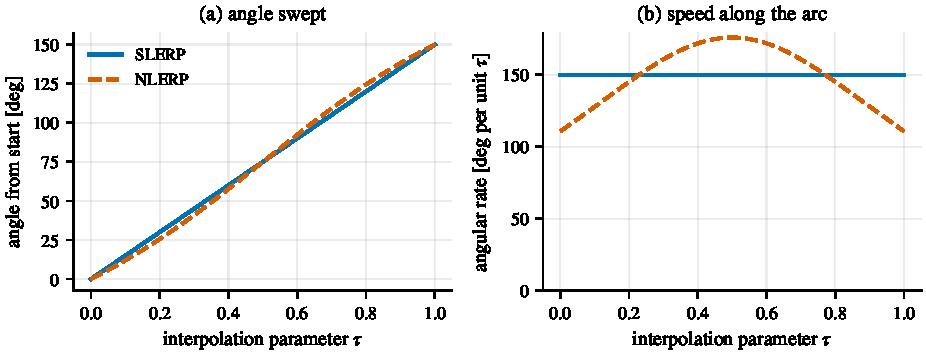
\includegraphics[width=0.84\textwidth]{fig_slerp.pdf}
  \caption{Interpolating between two attitudes $150^\circ$ apart. SLERP sweeps the angle uniformly in the interpolation parameter; normalized linear
  interpolation (NLERP) follows the same path but at a non-uniform speed, fastest in the middle.}
  \label{fig:slerp}
\end{figure}

Ground truth and IMU data rarely share timestamps with images, so attitudes must be interpolated. The correct interpolation follows the
shortest great arc at constant angular velocity: \term{spherical linear interpolation} (SLERP),
\begin{equation}
  q(\tau) = q_0 \qprod \Exp_q\!\big(\tau\,\Log_q(q_0\inv\qprod q_1)\big)
          = \frac{\sin((1 - \tau)\Omega)}{\sin\Omega}\,q_0 + \frac{\sin(\tau\Omega)}{\sin\Omega}\,q_1,
  \qquad \tau\in[0,1],
\end{equation}
with $\cos\Omega = q_0\T q_1$ after flipping the sign of $q_1$ if needed so that $q_0\T q_1 \ge 0$. The first form (using the exponential and
logarithm of \cref{ch:lie}) shows that the relative rotation is applied with a uniformly growing angle; the second is the formula for
interpolating along a great circle of the sphere. Component-wise linear interpolation followed by normalization (NLERP) follows the same
path at a non-uniform speed (\cref{fig:slerp}); it is acceptable only for small angles.

% ==============================================================================
\section{Rigid-body transformations}

A rigid transformation combines a rotation and a translation. Point coordinates transform as
\begin{equation}
  p_w = R_{wb}\,p_b + p_{wb}
  \quad\Longleftrightarrow\quad
  \begin{bmatrix} p_w \\ 1 \end{bmatrix} = \underbrace{\begin{bmatrix} R_{wb} & p_{wb} \\ 0 & 1 \end{bmatrix}}_{T_{wb}}
  \begin{bmatrix} p_b \\ 1 \end{bmatrix}.
\end{equation}
Appending a 1 to the point (\emph{homogeneous coordinates}, developed in \cref{ch:camera}) turns the affine map into a single matrix product.
The $4\times4$ matrices of this form make up the group $\SE$ of rigid motions. Composition and inversion follow from block multiplication:
\begin{equation}
  T_{wc} = T_{wb}T_{bc} = \begin{bmatrix} R_{wb}R_{bc} & R_{wb}p_{bc} + p_{wb} \\ 0 & 1\end{bmatrix},
  \qquad
  T_{wb}\inv = T_{bw} = \begin{bmatrix} R_{wb}\T & -R_{wb}\T p_{wb} \\ 0 & 1 \end{bmatrix}.
  \label{eq:se3-compose}
\end{equation}
The camera pose in the world therefore is $R_{wc} = R_{wb}R_{bc}$ and $p_{wc} = p_{wb} + R_{wb}p_{bc}$, and a world point $p_f$ has camera coordinates
\begin{equation}
  p_c = R_{bc}\T\big(R_{wb}\T(p_f - p_{wb}) - p_{bc}\big),
  \label{eq:world-to-camera}
\end{equation}
which is the first half of the camera measurement model (AGENTS.md C6).

\begin{pitfall}[points versus directions]
Translations apply to points, not to free vectors. A velocity, a gravity vector or a bearing direction transforms with the rotation only,
$v_w = R_{wb}v_b$. In homogeneous coordinates directions carry a $0$ in the fourth component, which drops the translation automatically.
\end{pitfall}

% ==============================================================================
\section{Rotational kinematics}
\label{sec:rot-kinematics}

\subsection{Angular velocity}

Let $R(t) = R_{wb}(t)$ describe a rotating body. Differentiating $R\T R = I$ gives $\dot R\T R + R\T\dot R = 0$, so $R\T\dot R$ is skew-symmetric and
equals $\sx{\omega_b}$ for a unique vector $\omega_b$:
\begin{equation}
  \dot R_{wb} = R_{wb}\,\sx{\omega_b} = \sx{\omega_w}\,R_{wb}, \qquad \omega_w = R_{wb}\,\omega_b ,
  \label{eq:rdot}
\end{equation}
where the second form uses \eqref{eq:skew-rot}. Why is $\omega$ an angular velocity? A point fixed in the body, with constant body coordinates $r_b$,
has world coordinates $r_w = R_{wb}r_b$ and velocity $\dot r_w = \dot R_{wb}r_b = \sx{\omega_w}R_{wb}r_b = \omega_w\times r_w$: every point moves as if the body
were spinning about the axis $\omega_w$ through the origin with angular speed $\|\omega\|$. $\omega_b$ is this angular velocity of $B$ relative to $W$,
expressed in $B$, and it is exactly what a strapdown gyroscope measures (up to bias and noise). The two forms of \eqref{eq:rdot} are the
kinematic origin of the two perturbation conventions of \cref{ch:lie}: a body-frame quantity multiplies on the right, a world-frame quantity on
the left.

\begin{proposition}[Constant body rate]
\label{prop:const-rate}
If $\omega_b$ is constant on $[t_0, t_0 + \Dt]$, then $R(t_0 + \Dt) = R(t_0)\exp(\Dt\sx{\omega_b})$.
\end{proposition}
\begin{proof}
$R(t) = R(t_0)\exp((t - t_0)\sx{\omega_b})$ satisfies \eqref{eq:rdot} by \cref{prop:matexp}, and the solution is unique (\cref{thm:lti-solution}).
\end{proof}

This exact solution is the basis of the multiplicative attitude update used in every integration scheme of \cref{ch:strapdown}. When the
rate varies, the update is still applied step by step with the rate held constant over each short step (\cref{sec:lie-euler}). Note that the
solution is \emph{not} $R(t_0) + \Dt\, R(t_0)\sx{\omega_b}$, which would leave $\SO$.

\subsection{Quaternion kinematics}

The quaternion counterpart of \eqref{eq:rdot} is
\begin{equation}
  \dot q_{wb} = \tfrac12\, q_{wb} \qprod [0,\ \omega_b] = \tfrac12\,\Omega(\omega_b)\,q_{wb},
  \qquad \Omega(\omega) = [\,[0, \omega]\,]_R = \begin{bmatrix} 0 & -\omega\T \\ \omega & -\sx{\omega}\end{bmatrix},
  \label{eq:qdot}
\end{equation}
with constant-rate solution $q(t_0 + \Dt) = q(t_0)\qprod\big[\cos\tfrac{\|\omega\|\Dt}{2},\ \sin\tfrac{\|\omega\|\Dt}{2}\,\tfrac{\omega}{\|\omega\|}\big]$. To derive
\eqref{eq:qdot}, compose $q(t + \dd t) = q(t) \qprod \dd q$, where $\dd q$ is the small body-frame rotation by $\omega_b\,\dd t$. By
\eqref{eq:quat-axis-angle}, $\dd q = [1,\ \tfrac12\omega_b\,\dd t] + O(\dd t^2)$, so $q(t + \dd t) - q(t) = q\qprod[0, \tfrac12\omega_b]\,\dd t$. The factor $\tfrac12$ is
the half angle again.

\subsection{Derivatives in a rotating frame}

Differentiating $v_w = R_{wb}v_b$ with \eqref{eq:rdot} gives the \term{transport theorem}
\begin{equation}
  \dot v_w = R_{wb}\big(\dot v_b + \omega_b \times v_b\big):
  \label{eq:transport}
\end{equation}
the rate of change seen from the fixed frame equals the rate seen in the rotating frame plus the change due to the rotation of the frame itself.
Applying it twice to the position $r$ of a particle relative to a frame rotating with angular velocity $\Omega$ (constant) gives the acceleration
in the fixed (inertial) frame, expressed in rotating coordinates:
\begin{equation}
  a_{\mathrm{inertial}} = \ddot r + 2\,\Omega\times\dot r + \Omega\times(\Omega\times r),
  \label{eq:coriolis}
\end{equation}
where $\ddot r$ and $\dot r$ are the acceleration and velocity seen in the rotating frame. The extra terms are the \term{Coriolis acceleration}
$2\Omega\times\dot r$ and the \term{centripetal acceleration} $\Omega\times(\Omega\times r)$. This formula is the working principle of the vibratory MEMS gyroscope
(\cref{ch:imu}), and it tells us what we neglect by treating the world frame as inertial.

\subsection{The Earth is not an inertial frame}

The world frame $W$ is fixed to the Earth, which rotates at $\Omega_e = 7.292\times10^{-5}$~rad/s. Three effects follow; their sizes justify the
project's simplifications.
\begin{itemize}
  \item \emph{Gyroscopes sense the Earth rate.} $7.3\times10^{-5}$~rad/s is comparable to the bias instability of the EuRoC ADIS16448 and far below its
        noise over short horizons. The project neglects it; its constant body-frame component (while the attitude changes little) is absorbed
        by the gyro bias estimate. High-grade systems model it explicitly and can even find north from it (gyrocompassing).
  \item \emph{Centripetal acceleration.} The term $\Omega_e\times(\Omega_e\times r)$ reaches $0.034~\mathrm{m/s^2}$ at the equator. It is absorbed into the
        local gravity vector: \emph{gravity}, as measured by a plumb line, is gravitation plus this centrifugal term. Its magnitude varies from
        $9.780~\mathrm{m/s^2}$ at the equator to $9.832~\mathrm{m/s^2}$ at the poles; the project uses a constant $9.81$ (AGENTS.md C5), accurate to about
        $10^{-3}$ relative in Zurich, where EuRoC was recorded.
  \item \emph{Coriolis acceleration.} $2\Omega_e\times v$ is about $1.5\times10^{-4}~\mathrm{m/s^2}$ at 1~m/s: below accelerometer noise and bias for a small
        drone, and neglected.
\end{itemize}
Over the minutes and hundreds of meters of a EuRoC sequence, the world frame may therefore be treated as inertial and flat, with constant
gravity.

\begin{takeaways}
\begin{itemize}
  \item $R_{wb}$ maps body coordinates to world coordinates; its columns are the body axes in the world. Adjacent subscripts must match.
  \item Every rotation is an axis-angle rotation, $R = I + \sin\theta\sx{u} + (1-\cos\theta)\sx{u}^2$; $\tr R = 1 + 2\cos\theta$.
  \item Euler angles have intrinsic and extrinsic readings and a singularity at $\pm90^\circ$ pitch; they stay out of the estimator.
  \item Hamilton unit quaternions compose like matrices; $q$ and $-q$ are the same rotation; the quaternion of a rotation by $\theta$ uses $\theta/2$.
  \item Eigen's constructor is $w$-first, its storage $w$-last, EuRoC is $w$-first. JPL formulas must be re-derived, not copied.
  \item $\dot R_{wb} = R_{wb}\sx{\omega_b}$; with constant $\omega_b$ the update $R \leftarrow R\exp(\Dt\sx{\omega_b})$ is exact.
  \item Derivatives in rotating frames pick up $\omega\times$ terms; for a small drone over minutes, the Earth's rotation is negligible.
\end{itemize}
\end{takeaways}

\begin{exercises}
  \item Show that the columns of any $R \in \SO$ are orthonormal and that $\det R = +1$ implies the third column is the cross product of the first two.
  \item Verify $R_x(90^\circ)R_y(90^\circ) \neq R_y(90^\circ)R_x(90^\circ)$ by computing both products, and describe each rotation physically.
  \item Derive \eqref{eq:euler-rates} from \eqref{eq:zyx} and $\sx{\omega_b} = R\T\dot R$.
  \item Convert the rotation of the worked example ($120^\circ$ about $(1,1,1)/\sqrt3$) to ZYX Euler angles.
  \item Prove that $[p]_L[q]_R = [q]_R[p]_L$. What does this say about associativity of the quaternion product?
  \item Show that $R(-q) = R(q)$ and compute the quaternion of a $270^\circ$ rotation about $z$ in its canonical form ($w \ge 0$). What rotation angle and
        axis does the canonical form describe?
  \item Implement Shepperd's method and test it on rotations by $0^\circ$, $90^\circ$, $179.9999^\circ$ and $180^\circ$.
  \item Write a function that converts a EuRoC ground-truth row into $p_{wb}$, $q_{wb}$, $v_{wb}$, $b_g$ and $b_a$. Design a fixture row whose values would
        expose a swapped $w/z$ and swapped biases.
  \item Given $T_{bc}$ from \code{cam0/sensor.yaml} (\cref{app:euroc}), compute the camera's optical axis in body coordinates.
  \item Show that if $\omega_b$ varies in time, $R(t) = R(0)\exp\big(\int_0^t\sx{\omega_b}\,\dd s\big)$ is in general \emph{wrong}. Construct a counterexample with
        piecewise-constant rates.
  \item Derive \eqref{eq:coriolis} by applying \eqref{eq:transport} twice.
\end{exercises}
\input{chapters/solutions/07_rotations}

\chapter{Lie Theory for Rotations}
\label{ch:lie}

\begin{objectives}
\begin{itemize}
  \item Understand $\SO$ as a curved manifold with a flat tangent space, and why an estimator needs both.
  \item Use the exponential and logarithm maps, in matrix and quaternion form, and implement them robustly.
  \item Distinguish local (right) and global (left) perturbations, and move perturbations across a
        rotation with the adjoint.
  \item Define Jacobians of functions of rotations, derive the right Jacobian $\Jr$, and build a table
        of elementary Jacobians from which every Jacobian in the project can be assembled.
  \item Represent and propagate uncertainty on $\SO$, and test manifold Jacobians numerically.
\end{itemize}
\end{objectives}

This chapter is the mathematical core of the notes. Its conclusions fit in a few lines (the
$\bplus$/$\bminus$ operators of \cref{sec:boxplus} and the Jacobian table of \cref{tab:jacobians}),
but the reasoning behind them is what lets you derive any new Jacobian correctly. The treatment
follows the ``micro Lie theory'' of Solà et al.~\cite{sola2018micro}, specialized to $\SO$ with the
conventions of this project. Barfoot~\cite{barfoot2017state} covers the same material in greater depth.

% ------------------------------------------------------------------------------
\section{Why estimation needs Lie theory}

A Kalman filter represents uncertainty as a mean and a covariance and corrects the mean by adding
a vector. Both operations assume the state lives in a vector space. Attitude does not.
\begin{itemize}
  \item \textbf{Addition leaves the space.} If $\hat q$ is a unit quaternion and $\delta q$ a small
        4-vector, $\hat q + \delta q$ is generally not unit length. The same holds for rotation matrices.
  \item \textbf{Redundant parameters give singular covariances.} A unit quaternion has four
        components but three degrees of freedom. A $4\times4$ covariance of a unit quaternion must be
        singular along the radial direction, and keeping it exactly singular under rounding is hopeless.
  \item \textbf{Minimal parameters have singularities.} Euler angles (\cref{ch:rotations}) are minimal
        but singular at gimbal lock.
\end{itemize}

\begin{keyidea}[the Earth and its tangent planes]
The surface of the Earth is curved, yet a town map drawn on flat paper is perfectly accurate for a
walk across town. The map is the \emph{tangent plane} at your location. It works as long as you do
not walk too far, and when you move to a new town you draw a new map. An estimator does the same:
it stores the attitude on the curved space $\SO$ (the globe), and expresses small uncertainties and
corrections in the flat 3D tangent space at the current estimate (the town map). The exponential
map turns a step on the map into a point on the globe, and the logarithm map does the reverse.
\end{keyidea}

% ------------------------------------------------------------------------------
\section{Warm-up: rotations of the plane}
\label{sec:so2}

Every idea of this chapter appears, in its simplest form, for planar rotations $R(\theta)$. Work through them here; the rest of the chapter
asks only what changes in three dimensions.
\begin{itemize}
  \item \emph{The set.} Planar rotations form a circle: $R(\theta)$ and $R(\theta + 2\pi)$ are the same. The set is one-dimensional but curved, and it is
        not a vector space ($R(\alpha) + R(\beta)$ is not a rotation).
  \item \emph{The tangent space.} Differentiating $R(\theta)$ at $\theta = 0$ gives $\frac{\dd R}{\dd\theta}(0) = \begin{bmatrix}0 & -1\\ 1 & 0\end{bmatrix}$; every velocity at the
        identity is a multiple of this skew-symmetric matrix. The tangent space is a line, coordinatized by a single number.
  \item \emph{Exponential and logarithm.} $\exp\big(\theta\begin{bmatrix}0 & -1\\ 1 & 0\end{bmatrix}\big) = R(\theta)$ (sum the series, or solve
        $\dot R = R\begin{bmatrix}0&-1\\1&0\end{bmatrix}$), so ``$\Exp$'' maps an angle to a rotation. Its inverse ``$\Log$'' recovers the angle,
        $\theta = \atantwo(R_{21}, R_{11}) \in (-\pi, \pi]$, unique only up to the choice of branch.
  \item \emph{Perturbations.} An estimate $R(\hat\theta)$ with a small error is $R(\hat\theta)R(\delta\theta) = R(\hat\theta + \delta\theta)$. Because planar rotations commute,
        perturbing on the left or on the right is the same, and the error of the composition is just the sum of the angles.
  \item \emph{Jacobians.} The derivative of $\Exp$ is the identity (1), and nothing like the right Jacobian appears.
\end{itemize}
In the plane, therefore, one can simply estimate the angle as a scalar, as long as differences are wrapped to $(-\pi, \pi]$. In three dimensions
rotations do not commute, the identity $R(\alpha)R(\beta) = R(\alpha + \beta)$ fails for rotation vectors with different axes, and left and right
perturbations differ. Each of these failures produces a new object in this chapter: the adjoint, the Baker--Campbell--Hausdorff formula, and the
right and left Jacobians.

% ------------------------------------------------------------------------------
\section{Manifolds, groups and Lie groups}

\subsection{Manifolds and tangent spaces}

\index{manifold}
A smooth $n$-dimensional \term{manifold} is a space that looks like $\R^n$ near every point. Precisely, each point has a neighborhood that can be
mapped smoothly and invertibly onto an open set of $\R^n$ (a \emph{chart}), and where two charts overlap, the change of coordinates between them is
smooth. The surface of a sphere is a 2D manifold: latitude and longitude form a chart away from the poles, and a second chart covers the poles. A
manifold usually needs several charts; a single chart for the whole sphere does not exist, and neither does one for $\SO$, which is why every
three-number parameterization of attitude has singularities.

A \term{tangent vector} at a point $x$ of a manifold is the velocity $\dot\gamma(0)$ of a smooth curve $\gamma(t)$ through $\gamma(0) = x$. The tangent vectors
at $x$ form a vector space, the \term{tangent space} $T_x\mathcal M$, of the same dimension as the manifold. For a manifold that sits inside a larger
vector space (as $\SO$ sits inside $\R^{3\times3}$), tangent vectors are ordinary vectors tangent to the surface: the tangent plane of a sphere
in the Earth analogy.

\subsection{Groups}

\begin{definition}[Group]
\index{group}
A \term{group} $(\mathcal{G}, \circ)$ is a set with an operation $\circ$ that is associative, has an identity element $\mathcal{E}$
($\mathcal{E}\circ\mathcal{X} = \mathcal{X}\circ\mathcal{E} = \mathcal{X}$), and an inverse $\mathcal{X}\inv$ for every element
($\mathcal{X}\circ\mathcal{X}\inv = \mathcal{E}$).
\end{definition}

Commutativity is \emph{not} required. Examples: $(\R^n, +)$ (identity $0$, inverse $-x$); the invertible $n\times n$ matrices under multiplication;
$\SO$; the unit quaternions under the Hamilton product; the rigid motions $\SE$. A group can also \emph{act} on another set: a rotation acts on
vectors by $v \mapsto Rv$, and a rigid motion acts on points by $p \mapsto Rp + t$. These actions are how groups enter measurement models.

\begin{definition}[Lie group]
\index{Lie group}
A \term{Lie group} is a group that is also a smooth manifold, such that composition and inversion are smooth maps. A \emph{matrix Lie group} is a
Lie group whose elements are invertible matrices and whose operation is matrix multiplication.
\end{definition}

Being a group as well gives a Lie group a remarkable property. Multiplication by a fixed element maps a neighborhood of the identity smoothly onto
a neighborhood of that element: the space looks the same everywhere. All local calculus can therefore be done once, at the identity, and
carried to any other element by composition. This is what makes estimation on $\SO$ tractable: one tangent space (at the identity), one
exponential map, and one set of Jacobian formulas serve every attitude.

\begin{center}\small
\begin{tabular}{@{}l l l l@{}}
\toprule
Group & Elements & Dimension & Role in VIO \\
\midrule
$(\R^n, +)$ & vectors & $n$ & position, velocity, biases \\
$\mathrm{SO}(2)$ & planar rotations & 1 & toy examples \\
$\SO$ & $3\times3$ rotation matrices & 3 & attitude \\
$S^3$ & unit quaternions & 3 & attitude (double cover of $\SO$) \\
$\SE$ & rigid transformations & 6 & poses, extrinsics \\
\bottomrule
\end{tabular}
\end{center}

% ------------------------------------------------------------------------------
\section{The Lie algebra and tangent spaces}

Consider a smooth curve $R(t) \in \SO$ with $R(0) = I$. Differentiating $R\T R = I$ at $t = 0$ gives
$\dot R(0)\T + \dot R(0) = 0$: the velocity at the identity is skew-symmetric. The set of all such
velocities is the \emph{Lie algebra}
\begin{equation}
  \so = \{\, \Omega \in \R^{3\times3} : \Omega\T = -\Omega \,\} = \{\, \sx{\phi} : \phi \in \R^3 \,\},
\end{equation}
a three-dimensional vector space identified with $\R^3$ by the hat and vee maps,
$\phi\hatop = \sx{\phi}$ and $\sx{\phi}\veeop = \phi$. Unlike $\SO$ itself, the Lie algebra is flat:
we can add its elements, scale them, and put Gaussian distributions on them.

\index{Lie bracket}
The Lie algebra carries one more operation, the \emph{Lie bracket} (commutator) $[X, Y] = XY - YX$, which measures how much two infinitesimal
motions fail to commute. The commutator of two skew-symmetric matrices is skew-symmetric, and by \eqref{eq:skew-commutator}
\begin{equation}
  \big[\sx{a}, \sx{b}\big] = \sx{a \times b} .
\end{equation}
So $\so$ with its bracket is $\R^3$ with the cross product. The cross product, which is zero only for parallel vectors, is the infinitesimal
version of the non-commutativity of rotations: rotations about parallel axes commute, all others do not.

At a general point $R$, the tangent space consists of the velocities of curves through $R$. From
\eqref{eq:rdot}, every such velocity can be written in two ways,
\begin{equation}
  \dot R = R\,\sx{\omega_b} = \sx{\omega_w}\,R, \qquad \omega_w = R\,\omega_b,
\end{equation}
so the tangent space at $R$ can be identified with $\R^3$ in two ways: by a vector expressed in the
\emph{local} (body) frame, multiplying on the right, or by a vector expressed in the \emph{global}
(world) frame, multiplying on the left. This is the origin of the two perturbation conventions of
\cref{sec:perturbations}. The project uses the local one.

\begin{figure}[t]
\centering
\begin{tikzpicture}[scale=1.0]
  % manifold surface
  \shade[top color=white, bottom color=primary!22] (0,0) ellipse (4.4 and 2.4);
  \draw[primary, thick] (0,0) ellipse (4.4 and 2.4);
  \draw[primary!50, dashed] (-4.4,0) arc (180:360:4.4 and 0.8);
  \node[primary, font=\small] at (-3.0,-1.5) {$\SO$};
  % tangent plane at Rhat
  \coordinate (X) at (-0.9,2.0);
  \fill[white, opacity=0.85, draw=black!55] ($(X)+(-2.4,0.35)$) -- ($(X)+(3.0,0.85)$) -- ($(X)+(3.6,-0.15)$) -- ($(X)+(-1.8,-0.65)$) -- cycle;
  \node[font=\small, anchor=west] at ($(X)+(-2.25,0.25)$) {$T_{\hat R}\SO \cong \R^3$};
  \fill[black] (X) circle (1.8pt) node[below=2pt] {$\hat R$};
  % the tangent vector
  \coordinate (V) at ($(X)+(2.4,0.3)$);
  \draw[->, very thick, plotorange] (X) -- (V) node[above=1pt, font=\small] {$\delta\theta$};
  % point on the manifold
  \coordinate (Y) at (2.4,0.9);
  \fill[plotgreen] (Y) circle (1.8pt);
  \node[plotgreen!70!black, below right=1pt, font=\small, fill=white, fill opacity=0.85, text opacity=1, inner sep=1.5pt, rounded corners=1pt] at (Y) {$\hat R\,\Exp(\delta\theta)$};
  \draw[->, plotgreen, thick, dashed] ($(V)+(0.05,-0.08)$) to[bend left=30] node[right=1pt, font=\footnotesize, pos=0.6] {$\Exp$} ($(Y)+(0.02,0.08)$);
  % logarithm back to the tangent space
  \draw[->, plotpurple, thick] ($(Y)+(-0.1,-0.05)$) to[bend left=25] node[below=1pt, font=\footnotesize] {$\Log(\hat R\T\,\cdot\,)$} ($(X)+(0.05,-0.12)$);
\end{tikzpicture}
\caption{The manifold $\SO$ and its tangent space at the estimate $\hat R$. A small error or correction
$\delta\theta \in \R^3$ lives in the flat tangent space. The exponential map wraps it onto the manifold as
$\hat R\Exp(\delta\theta)$, and the logarithm recovers it.}
\label{fig:tangent-space}
\end{figure}

% ------------------------------------------------------------------------------
\section{The exponential map}

\begin{definition}[Exponential map of $\SO$]
$\exp: \so \to \SO$ is the matrix exponential. Composed with the hat map it gives the
\emph{capitalized} exponential
\begin{equation}
  \Exp: \R^3 \to \SO, \qquad \Exp(\phi) = \exp(\sx{\phi}).
\end{equation}
By Rodrigues' formula (\cref{thm:rodrigues}), with $\theta = \|\phi\|$,
\begin{equation}
  \Exp(\phi) = I + \frac{\sin\theta}{\theta}\,\sx{\phi} + \frac{1 - \cos\theta}{\theta^2}\,\sx{\phi}^2 .
  \label{eq:Exp}
\end{equation}
\end{definition}

$\Exp(\phi)$ is the rotation by angle $\|\phi\|$ about the axis $\phi/\|\phi\|$. Its main properties are
$\Exp(0) = I$, $\Exp(-\phi) = \Exp(\phi)\T$, and $\Exp(s\phi)\Exp(t\phi) = \Exp((s+t)\phi)$: rotations about a
\emph{common} axis compose by adding angles. $\Exp$ is onto $\SO$, and one-to-one on the open ball
$\|\phi\| < \pi$.

\paragraph{Why the exponential?} The curve $R(t) = \Exp(t\phi)$ is the motion of a body spinning at the constant body rate $\phi$: it solves
$\dot R = R\sx{\phi}$ with $R(0) = I$ (\cref{prop:const-rate}), and it is a \emph{one-parameter subgroup}, $R(s)R(t) = R(s + t)$. The exponential
map thus sends each tangent vector at the identity to the point reached by moving ``straight'' in that direction for unit time. In every Lie
group, the exponential is defined the same way, which is why the same machinery works for $\SO$, $\SE$ and the extended poses used by
invariant filters.

\paragraph{Quaternion exponential.} The unit quaternion corresponding to $\Exp(\phi)$ follows from
\eqref{eq:quat-axis-angle}:
\begin{equation}
  \Exp_q(\phi) = \begin{bmatrix} \cos(\theta/2) \\ \dfrac{\sin(\theta/2)}{\theta}\,\phi \end{bmatrix},
  \qquad R\big(\Exp_q(\phi)\big) = \Exp(\phi).
  \label{eq:Expq}
\end{equation}
This is the quaternion exponential of the pure quaternion $[0, \phi/2]$; the half angle is the double
cover again. Since $\Exp_q(\phi)$ has $w = \cos(\theta/2) \ge 0$ for $\theta \le \pi$, its output is
already in canonical form on that range.

\subsection{Numerical evaluation and the Taylor branches}
\label{sec:taylor}

Formulas \eqref{eq:Exp} and \eqref{eq:Expq}, and the Jacobian formulas later in this chapter, are built
from a handful of scalar \emph{coefficient functions} of $\theta$:
\begin{equation}
  A(\theta) = \frac{\sin\theta}{\theta},\quad
  B(\theta) = \frac{1-\cos\theta}{\theta^2},\quad
  C(\theta) = \frac{\theta - \sin\theta}{\theta^3},\quad
  D(\theta) = \frac{1}{\theta^2} - \frac{\cot(\theta/2)}{2\theta}.
\end{equation}
All four are smooth, even functions with finite limits at $\theta = 0$, but their formulas read $0/0$
there. Their Taylor series are
\begin{equation}
\begin{aligned}
  A &= 1 - \tfrac{\theta^2}{6} + \tfrac{\theta^4}{120} - \cdots, &
  B &= \tfrac12 - \tfrac{\theta^2}{24} + \tfrac{\theta^4}{720} - \cdots, \\
  C &= \tfrac16 - \tfrac{\theta^2}{120} + \tfrac{\theta^4}{5040} - \cdots, &
  D &= \tfrac1{12} + \tfrac{\theta^2}{720} + \tfrac{\theta^4}{30240} + \cdots,
\end{aligned}
\label{eq:coeff-taylor}
\end{equation}
and for the quaternion map
$\cos\frac\theta2 = 1 - \frac{\theta^2}{8} + \frac{\theta^4}{384} - \cdots$ and
$\frac{\sin(\theta/2)}{\theta} = \frac12 - \frac{\theta^2}{48} + \frac{\theta^4}{3840} - \cdots$.

There are two distinct numerical issues.
\begin{enumerate}
  \item \textbf{Division by zero.} At $\theta = 0$ exactly (a perfectly still IMU, or a zero
        correction), every formula evaluates to \code{NaN}, and a single \code{NaN} propagates through
        $P$ and destroys the filter. For tiny $\theta$, $\theta^2$ can also underflow to zero.
  \item \textbf{Cancellation.} $B$, $C$ and $D$ subtract nearly equal quantities. As
        \cref{fig:taylor}(a) shows, their naive evaluation has relative error of order $u/\theta^2$:
        about $10^{-8}$ at $\theta = 10^{-4}$, and complete loss below $\theta \approx 10^{-8}$.
        $A$ and the quaternion coefficients involve no subtraction and are accurate everywhere except at
        $0/0$.
\end{enumerate}

\begin{figure}[t]
  \centering
  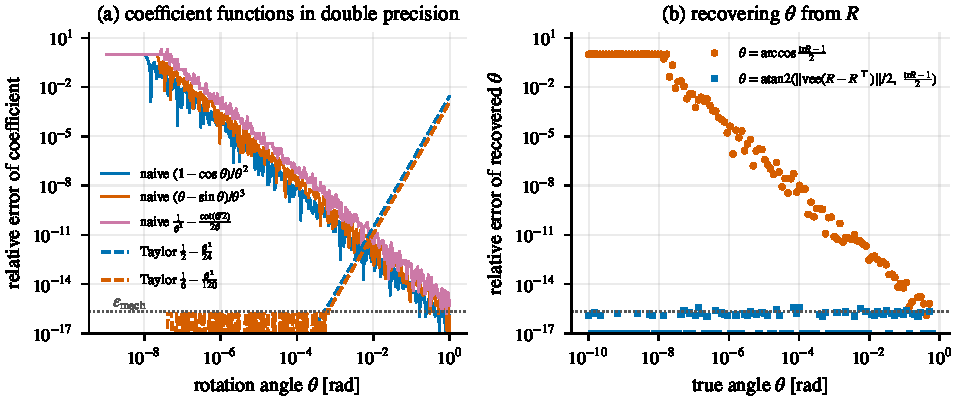
\includegraphics[width=\textwidth]{fig_taylor.pdf}
  \caption{(a) Relative error of the coefficient functions evaluated naively in double precision
  (solid) and with a two-term Taylor series (dashed), against a 60-digit reference. The naive error
  grows like $u/\theta^2$ as $\theta\to0$, and the truncation error of the series grows like $\theta^4$.
  (b) Recovering the angle from a rotation matrix: $\arccos$ loses accuracy like $u/\theta^2$ and
  returns exactly zero below $10^{-8}$, while the $\atantwo$ form is accurate to machine precision at
  every angle.}
  \label{fig:taylor}
\end{figure}

How much does the cancellation matter? It depends on what the coefficient multiplies. A coefficient
with absolute error $\epsilon_c$ that multiplies $\sx{\phi}^k$ contributes an error of about
$\epsilon_c\theta^k$ to the matrix. For $B$, $C$ and $D$, $\epsilon_c \approx u/\theta^2$, so:
\begin{center}\small
\begin{tabular}{@{}l l c l@{}}
\toprule
Function & cancelling coefficient & multiplies & naive absolute error \\
\midrule
$\Exp(\phi)$ & $B$ & $\sx{\phi}^2$ & $\approx u$ \quad (harmless) \\
$\Jr(\phi)$ & $B$ & $\sx{\phi}$ & $\approx u/\theta$ \quad (\textbf{harmful}: $3\times10^{-9}$ at $\theta = 10^{-8}$) \\
$\Jr(\phi)$ & $C$ & $\sx{\phi}^2$ & $\approx u$ \\
$\Jrinv(\phi)$ & $D$ & $\sx{\phi}^2$ & $\approx u$ \\
\bottomrule
\end{tabular}
\end{center}

\begin{keyidea}[why the Taylor branch exists, and how to choose its threshold]
Every function needs a guard against $0/0$. Beyond that, the branch matters for accuracy wherever a
cancelling coefficient multiplies a low power of $\sx{\phi}$, as in $\Jr$. To choose the threshold
$\theta_0$ and the number of terms, balance the two error curves of \cref{fig:taylor}(a): keeping terms
through $\theta^{2m}$ leaves a truncation error of order $\theta^{2m+2}$, and the exact formula has a
rounding error of order $u/\theta^2$. Below the crossing point use the series, above it the formula.
For two-term series ($m = 1$) the curves cross near $\theta \approx 3\times10^{-3}$, where both relative
errors are about $10^{-12}$; adding the $\theta^4$ term moves the crossing to larger angles and lowers
the error there. Remember to multiply by $\theta^k$ when translating a coefficient error into a matrix
error. Record the choice and this justification next to the code (Milestone 2).
\end{keyidea}

% ------------------------------------------------------------------------------
\section{The logarithm map}
\label{sec:log}

\begin{definition}[Logarithm map]
$\Log: \SO \to \R^3$ returns the rotation vector $\phi$ with $\|\phi\| \le \pi$ such that
$\Exp(\phi) = R$.
\end{definition}

For angles strictly between $0$ and $\pi$ the answer is unique. Combining the two equations of
\eqref{eq:trace-angle},
\begin{equation}
  \theta = \atantwo\!\Big( \tfrac12\big\|(R - R\T)\veeop\big\|,\ \tfrac12(\tr R - 1) \Big), \qquad
  \Log(R) = \frac{\theta}{2\sin\theta}\,(R - R\T)\veeop .
  \label{eq:Log}
\end{equation}
The $\atantwo$ form is essential. The common textbook formula $\theta = \arccos\big((\tr R - 1)/2\big)$ is
correct mathematically but numerically unstable near $\theta = 0$, where $\arccos$ has infinite slope,
and loses half the significant digits (\cref{fig:taylor}b). Three regimes need care in code.

\begin{enumerate}
  \item \textbf{Small angles.} $\theta/(2\sin\theta) \to \tfrac12$, so use
        $\Log(R) \approx \tfrac12(1 + \tfrac{\theta^2}{6})(R - R\T)\veeop$.
  \item \textbf{Generic angles.} Use \eqref{eq:Log} directly.
  \item \textbf{Angles near $\pi$.} $\sin\theta \to 0$ and $(R - R\T)\veeop = 2\sin\theta\,u$ vanishes, so
        the axis cannot be recovered from the skew-symmetric part. Use the symmetric part instead: from
        \eqref{eq:rodrigues}, $\tfrac12(R + R\T) = \cos\theta\,I + (1-\cos\theta)\,uu\T$, so
        $uu\T = \big(\tfrac12(R + R\T) - \cos\theta\, I\big)/(1 - \cos\theta)$. Take the column with the largest
        diagonal entry, normalize it to get $\pm u$, and fix the sign so that $u\T(R - R\T)\veeop \ge 0$.
\end{enumerate}

\begin{figure}[t]
\centering
\begin{tikzpicture}[scale=1.0]
  \fill[primarylight] (0,0) circle (2.0);
  \draw[primary, thick] (0,0) circle (2.0);
  \fill (0,0) circle (1.4pt) node[below right] {$I$};
  \draw[->, thick, plotorange] (0,0) -- (1.2,0.8) node[above right=-2pt] {$\phi$};
  \fill[plotgreen] (40:2.0) circle (2pt) node[above right] {$\pi u$};
  \fill[plotgreen] (220:2.0) circle (2pt) node[below left] {$-\pi u$};
  \draw[plotgreen, dashed, <->] (40:1.9) -- (220:1.9);
  \draw[->, plotpurple, thick] (-0.3,-1.2) .. controls (0.6,-1.4) and (1.4,-1.5) .. (330:2.0);
  \draw[->, plotpurple, thick] (150:2.0) .. controls (-1.2,0.6) .. (-0.6,0.4);
  \node[plotpurple, font=\footnotesize, align=left] at (3.6,-1.1) {a path leaving the ball\\re-enters at the\\antipodal point};
  \node[primary, font=\footnotesize] at (0,2.35) {$\|\phi\| \le \pi$};
\end{tikzpicture}
\caption{$\SO$ pictured as the ball of rotation vectors of radius $\pi$, with antipodal points on the
boundary identified ($\pi u$ and $-\pi u$ are the same rotation). $\Log$ is smooth inside the ball but
must jump when a rotation crosses $\theta = \pi$. Near the boundary a tiny change in $R$ can flip the
returned vector to the opposite side.}
\label{fig:so3-ball}
\end{figure}

\begin{remark}[why $\Log$ is ill-conditioned near $\pi$]
Near $\theta = \pi$ two different effects combine. Algebraically, the axis must be extracted from a
nearly vanishing skew-symmetric part, so the na\"ive formula amplifies rounding errors by
$1/\sin\theta$. Topologically, $\Log$ is discontinuous at $\theta = \pi$ (\cref{fig:so3-ball}): a
rotation by $\pi - \epsilon$ about $u$ and one by $\pi - \epsilon$ about $-u$ are close in $\SO$ but have
$\Log$ values $2\pi$ apart. No implementation can remove the second effect. In an estimator it rarely
matters, because $\Log$ is applied to \emph{differences} between nearby rotations, whose angles are
small. Milestone 2 nevertheless tests the near-$\pi$ regime, because a broken branch there produces
\code{NaN}.
\end{remark}

\paragraph{Quaternion logarithm.} For a unit quaternion $q = [w, v]$, first canonicalize to $w \ge 0$ (replace
$q$ by $-q$ if needed), then
\begin{equation}
  \Log_q(q) = 2\,\atantwo(\|v\|, w)\,\frac{v}{\|v\|}
  \ \approx\ \frac{2}{w}\Big(1 - \frac{\|v\|^2}{3w^2}\Big)\,v \quad\text{for small }\|v\|.
  \label{eq:Logq}
\end{equation}
Canonicalization guarantees $\|\Log_q(q)\| \le \pi$ and makes $\Log_q(q) = \Log_q(-q)$, so the double cover is
invisible to the estimator. The $\atantwo$ is well-conditioned at all angles, including near $\pi$ where
$w \approx 0$: the quaternion logarithm does not suffer the algebraic ill-conditioning of the matrix version.
The topological discontinuity at $\pi$ remains.

% ------------------------------------------------------------------------------
\section{The adjoint: moving a perturbation across a rotation}

\begin{proposition}[Adjoint of $\SO$]
\label{prop:adjoint}
For all $R \in \SO$ and $\phi \in \R^3$,
\begin{equation}
  R\,\Exp(\phi)\,R\T = \Exp(R\phi),
  \label{eq:adjoint}
\end{equation}
or equivalently $\Exp(\phi)\,R = R\,\Exp(R\T\phi)$ and $R\,\Exp(\phi) = \Exp(R\phi)\,R$.
\end{proposition}
\begin{proof}
By \eqref{eq:skew-rot}, $R\sx{\phi}R\T = \sx{R\phi}$. By property 4 of \cref{prop:matexp},
$R\exp(\sx{\phi})R\T = \exp(R\sx{\phi}R\T) = \exp(\sx{R\phi})$. The equivalent forms follow by
multiplying on the right or left by $R$ or $R\T$.
\end{proof}

The map $\phi \mapsto R\phi$ is the \emph{adjoint action} $\Ad_R$, which for $\SO$ is simply the rotation
matrix itself. Geometrically, a rotation about an axis $\phi$ expressed in one frame equals the rotation
about the same physical axis expressed in another frame. \Cref{eq:adjoint} is the single most used identity
in Jacobian derivations: it lets you slide a perturbation $\Exp(\delta)$ through other rotations until
it reaches the position the convention requires.

% ------------------------------------------------------------------------------
\section{Composition and the Baker--Campbell--Hausdorff formula}

Rotations about different axes do not commute, so $\Exp(a)\Exp(b) \neq \Exp(a + b)$ in general. The
Baker--Campbell--Hausdorff (BCH) formula quantifies the discrepancy. For matrices $X, Y$ near zero,
\begin{equation}
  \log\big(\exp X \exp Y\big) = X + Y + \tfrac12[X, Y] + \tfrac1{12}\big([X,[X,Y]] + [Y,[Y,X]]\big) + \cdots,
\end{equation}
where $[X, Y] = XY - YX$. For $\so$, \eqref{eq:skew-commutator} gives $[\sx{a}, \sx{b}] = \sx{a\times b}$, so
\begin{equation}
  \Log\big(\Exp(a)\Exp(b)\big) = a + b + \tfrac12\, a\times b
     + \tfrac1{12}\big( a\times(a\times b) + b\times(b\times a)\big) + \cdots .
  \label{eq:bch}
\end{equation}

\begin{proof}[Derivation of the second-order term]
Expand both exponentials to second order: $\exp X\exp Y = (I + X + \tfrac12X^2)(I + Y + \tfrac12Y^2) + O(3) = I + X + Y + \tfrac12X^2 + XY + \tfrac12Y^2 + O(3)$,
where $O(3)$ collects terms of third order in $X$ and $Y$. Write the result as $\exp Z$ with $Z = X + Y + Z_2 + O(3)$ and $Z_2$ of second order. Then
$\exp Z = I + Z + \tfrac12Z^2 + O(3) = I + X + Y + Z_2 + \tfrac12(X + Y)^2 + O(3)$. Comparing the two expansions,
$Z_2 = \tfrac12X^2 + XY + \tfrac12Y^2 - \tfrac12(X^2 + XY + YX + Y^2) = \tfrac12(XY - YX)$. The higher-order terms are obtained the same way, with
more patience; they involve only nested brackets, a theorem in itself.
\end{proof}
The first correction is second order. Two small rotations therefore compose approximately additively,
$\Exp(a)\Exp(b) \approx \Exp(a + b)$, with an error of order $\|a\|\|b\|$. When only one of them is small,
summing the BCH series in the large argument gives the two most important first-order formulas of
this chapter:
\begin{align}
  \Log\big(\Exp(\phi)\,\Exp(\delta)\big) &= \phi + \Jrinv(\phi)\,\delta + O(\|\delta\|^2), \label{eq:bch-right}\\
  \Log\big(\Exp(\delta)\,\Exp(\phi)\big) &= \phi + \Jlinv(\phi)\,\delta + O(\|\delta\|^2), \label{eq:bch-left}
\end{align}
with the Jacobians $\Jr$ and $\Jl$ defined in \cref{sec:jr}.

% ------------------------------------------------------------------------------
\section{Perturbations, \texorpdfstring{$\bplus$}{boxplus} and \texorpdfstring{$\bminus$}{boxminus}}
\label{sec:perturbations}
\label{sec:boxplus}

Let $\hat R$ be an estimate and $R$ the truth. There are two natural ways to write the small rotation
separating them:
\begin{equation}
  \underbrace{R = \hat R\,\Exp(\delta\theta_b)}_{\text{local (right) perturbation}}
  \qquad\qquad
  \underbrace{R = \Exp(\delta\theta_w)\,\hat R}_{\text{global (left) perturbation}} .
\end{equation}
By \cref{prop:adjoint} they describe the same error, related by $\delta\theta_w = \hat R\,\delta\theta_b$.
$\delta\theta_b$ is the error expressed in the estimated body frame, $\delta\theta_w$ the same error expressed in
the world frame. If $\delta\theta_b \sim \N(0, P_b)$, then $\delta\theta_w \sim \N(0, \hat R P_b \hat R\T)$.

\begin{figure}[t]
\centering
\begin{tikzpicture}[scale=1.0]
  % world frame
  \draw[frameaxis, black!60] (0,0) -- (1.1,0) node[right, font=\footnotesize] {$x_w$};
  \draw[frameaxis, black!60] (0,0) -- (0,1.1) node[above, font=\footnotesize] {$z_w$};
  \node[below left, font=\footnotesize] at (0,0) {$W$};
  % estimated and true body frames
  \begin{scope}[shift={(3.4,0.2)}]
    \begin{scope}[rotate=25]
      \draw[frameaxis, primary] (0,0) -- (1.5,0) node[right, font=\footnotesize] {$\hat x_b$};
      \draw[frameaxis, primary] (0,0) -- (0,1.5) node[above left=-2pt, font=\footnotesize] {$\hat z_b$};
    \end{scope}
    \begin{scope}[rotate=45]
      \draw[frameaxis, plotorange, dashed] (0,0) -- (1.5,0) node[above right=-1pt, font=\footnotesize] {$x_b$};
      \draw[frameaxis, plotorange, dashed] (0,0) -- (0,1.5) node[above left=-2pt, font=\footnotesize] {$z_b$};
    \end{scope}
    \draw[->, plotgreen, thick] (25:1.05) arc (25:45:1.05);
    \node[plotgreen, font=\footnotesize] at (35:1.45) {$\delta\theta_b$};
    \node[font=\footnotesize, align=center, below=4pt] at (0.4,0) {estimated frame $\hat R$ (solid)\\ and true frame $R$ (dashed)};
  \end{scope}
  % summary box
  \node[draw=conv, fill=convlight, rounded corners, align=left, font=\footnotesize, text width=5.4cm, anchor=west] at (6.6,0.6) {
    Local: $R = \hat R\Exp(\delta\theta_b)$ \textbf{(this project)}\\[2pt]
    Global: $R = \Exp(\delta\theta_w)\hat R$\\[2pt]
    Same error: $\delta\theta_w = \hat R\,\delta\theta_b$\\[2pt]
    Covariances: $P_w = \hat R P_b \hat R\T$};
\end{tikzpicture}
\caption{The local (right) perturbation measures the attitude error as a small rotation about the axes of
the \emph{estimated} body frame. The global (left) perturbation measures the same error about the world
axes.}
\label{fig:perturbations}
\end{figure}

Both conventions are mathematically valid and widely used, but they are not interchangeable. Every
Jacobian, covariance and residual depends on the choice. The project uses the local one for three
reasons.
\begin{enumerate}
  \item \textbf{It matches the sensor.} The gyroscope measures $\omega_b$ in the body frame and
        \eqref{eq:rdot} puts it on the right, so body-frame errors couple to body-frame quantities.
  \item \textbf{It is decoupled from global yaw.} The local attitude error dynamics
        (\cref{ch:errordyn}) depend on $\hat\omega$ and the biases but not on the absolute heading.
  \item \textbf{It is the convention of the standard ESKF reference~\cite{sola2017quaternion}}, which makes
        the literature easy to cross-check.
\end{enumerate}

\begin{convention}[retraction and local difference, AGENTS.md C4]
For the full state $x = (p, v, q, b_a, b_g, \{p_i, q_i\})$ and $\delta x \in \R^{15 + 6N}$:
\begin{align*}
  x = \hat x \bplus \delta x:&\quad p = \hat p + \delta p,\quad v = \hat v + \delta v,\quad
       q = \hat q\qprod\Exp_q(\delta\theta),\quad b = \hat b + \delta b, \\
  \delta x = x \bminus \hat x:&\quad \delta\theta = \Log_q(\hat q\inv\qprod q),\quad\text{all other blocks subtract.}
\end{align*}
Clone blocks follow the same rule. Every residual, Jacobian, injection and numerical-differentiation test
uses these two operators and nothing else.
\end{convention}

The operators satisfy the axioms that make them a consistent local parameterization:
\begin{equation}
  x \bplus 0 = x, \qquad (x \bplus \delta) \bminus x = \delta, \qquad x \bplus (y \bminus x) = y,
\end{equation}
the second for $\|\delta\theta\| < \pi$ and the third for any $y$. The state is a \emph{product manifold}
$\R^3\times\R^3\times\SO\times\R^3\times\R^3\times(\R^3\times\SO)^N$. Each factor has its own
$\bplus$, and the composite operator acts block-wise.

% ------------------------------------------------------------------------------
\section{Jacobians on manifolds}
\label{sec:jr}

\begin{definition}[Jacobian with respect to local perturbations]
\label{def:manifold-jacobian}
Let $f: \mathcal{M} \to \mathcal{N}$ map between manifolds with $\bplus$/$\bminus$ operators. Its
Jacobian at $x$ is the matrix
\begin{equation}
  J^f_x = \frac{\partial}{\partial\delta}\Big[ f(x\bplus\delta) \bminus f(x) \Big]_{\delta = 0},
  \qquad\text{so that}\qquad f(x\bplus\delta) = f(x)\bplus\big(J^f_x\,\delta + O(\|\delta\|^2)\big).
  \label{eq:manifold-jacobian}
\end{equation}
\end{definition}

When both spaces are vector spaces this is the ordinary Jacobian. The chain rule holds unchanged,
$J^{g\circ f}_x = J^g_{f(x)}\,J^f_x$, so complicated Jacobians are products of simple ones. The column
$j$ of $J^f_x$ is what a finite-difference test computes by perturbing direction $j$, which is how every
such Jacobian is verified.

\subsection{The right and left Jacobians of \texorpdfstring{$\SO$}{SO(3)}}

\begin{definition}[Right and left Jacobians]
The \emph{right Jacobian} $\Jr(\phi)$ is the Jacobian of $\Exp: \R^3 \to \SO$ with the local $\bminus$ on
$\SO$; the \emph{left Jacobian} $\Jl(\phi)$ uses the global one:
\begin{equation}
  \Exp(\phi + \delta) = \Exp(\phi)\,\Exp\big(\Jr(\phi)\,\delta\big) + O(\|\delta\|^2)
  = \Exp\big(\Jl(\phi)\,\delta\big)\,\Exp(\phi) + O(\|\delta\|^2).
  \label{eq:jr-def}
\end{equation}
\end{definition}

$\Jr(\phi)$ answers the question: if I change the rotation \emph{vector} $\phi$ by $\delta$, what small
\emph{body-frame} rotation does the rotation \emph{matrix} undergo? Only for $\phi = 0$ is the answer
$\delta$ itself.

\begin{theorem}[Closed forms]
\label{thm:jr}
With $\theta = \|\phi\|$,
\begin{align}
  \Jr(\phi) &= \int_0^1 \Exp(-s\phi)\,\dd s
             = I - \frac{1-\cos\theta}{\theta^2}\,\sx{\phi} + \frac{\theta - \sin\theta}{\theta^3}\,\sx{\phi}^2, \label{eq:jr}\\
  \Jrinv(\phi) &= I + \tfrac12\sx{\phi} + \Big(\frac{1}{\theta^2} - \frac{1 + \cos\theta}{2\theta\sin\theta}\Big)\sx{\phi}^2, \label{eq:jrinv}\\
  \Jl(\phi) &= \Jr(-\phi) = \Jr(\phi)\T = \Exp(\phi)\,\Jr(\phi), \qquad \Jlinv(\phi) = \Jrinv(-\phi). \label{eq:jl}
\end{align}
The coefficient in \eqref{eq:jrinv} equals $D(\theta) = \frac{1}{\theta^2} - \frac{\cot(\theta/2)}{2\theta}$,
which is finite at $\theta = \pi$ (where $D = 1/\pi^2$) and singular only at $\theta = 2\pi$.
\end{theorem}
\begin{proof}
\emph{Step 1: the derivative of the matrix exponential.} Let $K(t) = \exp\big(t(X + \epsilon Y)\big)$, which solves
$\dot K = (X + \epsilon Y)K$, $K(0) = I$. Its derivative with respect to $\epsilon$ at $\epsilon = 0$, $W(t) = \partial K/\partial\epsilon$, solves the equation obtained by
differentiating the ODE: $\dot W = XW + Y\exp(tX)$, $W(0) = 0$. This is a linear ODE with an input, so by variation of constants
(\cref{prop:stm}) $W(t) = \int_0^t\exp((t - s)X)\,Y\exp(sX)\,\dd s$. At $t = 1$, after substituting $s \to 1 - s$,
\begin{equation*}
  \frac{\dd}{\dd\epsilon}\exp(X + \epsilon Y)\Big|_{\epsilon=0} = \int_0^1 \exp(sX)\,Y\exp((1-s)X)\,\dd s .
\end{equation*}
\emph{Step 2: the integral form.} With $X = \sx{\phi}$ and $Y = \sx{\delta}$,
\begin{align*}
  \Exp(\phi)\inv\,\frac{\dd}{\dd\epsilon}\Exp(\phi + \epsilon\delta)\Big|_0
  &= \int_0^1 \Exp(-(1-s)\phi)\,\sx{\delta}\,\Exp((1-s)\phi)\,\dd s \\
  &= \Big[\int_0^1 \Exp(-s\phi)\,\dd s\ \delta\Big]_\times,
\end{align*}
using $R\sx{\delta}R\T = \sx{R\delta}$ with $R = \Exp(-(1-s)\phi)$ and substituting $s \to 1 - s$ again. Comparing with
$\Exp(\phi)\Exp(\epsilon\Jr\delta) = \Exp(\phi)(I + \epsilon\sx{\Jr\delta}) + O(\epsilon^2)$ gives $\Jr(\phi) = \int_0^1\Exp(-s\phi)\,\dd s$.

\emph{Step 3: the closed form.} With $u = \phi/\theta$, Rodrigues' formula gives
$\Exp(-s\phi) = I - \sin(s\theta)\sx{u} + (1 - \cos(s\theta))\sx{u}^2$. Integrating term by term, $\int_0^1\sin(s\theta)\,\dd s = (1 - \cos\theta)/\theta$ and
$\int_0^1(1 - \cos(s\theta))\,\dd s = 1 - \sin\theta/\theta$, so
$\Jr = I - \frac{1 - \cos\theta}{\theta}\sx{u} + \big(1 - \frac{\sin\theta}{\theta}\big)\sx{u}^2$; substituting $\sx{u} = \sx{\phi}/\theta$ gives \eqref{eq:jr}.

\emph{Step 4: the inverse.} Write $K = \sx{\phi}$, $\Jr = I - BK + CK^2$ with the coefficients $B$ and $C$ of \eqref{eq:jr}, and look for the inverse in the
same form, $I + aK + bK^2$. Multiplying out and reducing $K^3 = -\theta^2K$ and $K^4 = -\theta^2K^2$, the product equals $I$ exactly when
\begin{equation*}
  a - B + \theta^2(bB - aC) = 0, \qquad b - aB + C - \theta^2bC = 0 .
\end{equation*}
These two linear equations have the solution $a = \tfrac12$ and $b = D(\theta)$ (substitute the trigonometric expressions and simplify, or
check numerically), which is \eqref{eq:jrinv}; the identity $\frac{1+\cos\theta}{\sin\theta} = \cot\frac\theta2$ gives the form of $D$.

\emph{Step 5: the left Jacobian.} By \cref{prop:adjoint}, $\Exp(\phi)\Exp(\Jr\delta) = \Exp(\Exp(\phi)\Jr\delta)\Exp(\phi)$, so $\Jl = \Exp(\phi)\Jr$. Repeating
steps 1--3 with the perturbation on the left gives $\Jl = \int_0^1\Exp(s\phi)\,\dd s$, which is $\Jr(-\phi)$ and, since $\Exp(s\phi)\T = \Exp(-s\phi)$,
also $\Jr(\phi)\T$.
\end{proof}

The small-angle expansions are $\Jr(\phi) = I - \tfrac12\sx{\phi} + \tfrac16\sx{\phi}^2 + O(\theta^3)$ and
$\Jrinv(\phi) = I + \tfrac12\sx{\phi} + \tfrac1{12}\sx{\phi}^2 + O(\theta^4)$, with the coefficient series of
\eqref{eq:coeff-taylor}. Equations \eqref{eq:bch-right} and \eqref{eq:bch-left} follow from
\eqref{eq:jr-def} by inverting the relation.

\subsection{Elementary Jacobians}

\begin{table}[t]
\centering\small
\renewcommand{\arraystretch}{1.35}
\begin{tabular}{@{}l l l@{}}
\toprule
Function & Jacobian w.r.t.\ local perturbation & Note \\
\midrule
$f(R) = Rv$ & $\dfrac{\partial f}{\partial\delta\theta} = -R\sx{v}$ & rotate a body vector to world \\
$f(R) = R\T v$ & $\dfrac{\partial f}{\partial\delta\theta} = \sx{R\T v}$ & express a world vector in body \\
$f(R) = R\inv$ & $J = -R$ & output on $\SO$ (local) \\
$f(R_1, R_2) = R_1R_2$ & $J_{R_1} = R_2\T$, \quad $J_{R_2} = I$ & output on $\SO$ (local) \\
$f(\phi) = \Exp(\phi)$ & $J = \Jr(\phi)$ & vector to $\SO$ \\
$f(R) = \Log(R)$ & $J = \Jrinv(\Log R)$ & $\SO$ to vector \\
$f(\phi) = \Exp(\phi)\,v$ & $\dfrac{\partial f}{\partial\phi} = -\Exp(\phi)\sx{v}\Jr(\phi)$ & rotation vector acting on $v$ \\
$f(v) = Rv$ & $J = R$ & ordinary linear map \\
\bottomrule
\end{tabular}
\caption{Elementary Jacobians with respect to the local (right) perturbation $R \to R\Exp(\delta\theta)$. All
other Jacobians in these notes are products of these by the chain rule. Each entry has been checked
numerically by central differences.}
\label{tab:jacobians}
\end{table}

The entries of \cref{tab:jacobians} are derived in two or three lines each. The method is always the same:
\textbf{perturb, expand to first order, isolate the perturbation, and read off the coefficient.}

\begin{example}[Rotation action]
\label{ex:rotation-action}
For $f(R) = Rv$: $f(R\Exp(\delta\theta)) = R(I + \sx{\delta\theta})v + O(\|\delta\theta\|^2) = Rv + R\sx{\delta\theta}v$.
By \eqref{eq:skew-anticomm}, $\sx{\delta\theta}v = -\sx{v}\delta\theta$, so the Jacobian is $-R\sx{v}$.
\end{example}

\begin{example}[Inverse action]
For $f(R) = R\T v$: $(R\Exp(\delta\theta))\T v = \Exp(-\delta\theta)R\T v \approx (I - \sx{\delta\theta})R\T v =
R\T v + \sx{R\T v}\,\delta\theta$.
\end{example}

\begin{example}[Inverse and composition]
For $f(R) = R\inv$: $(R\Exp(\delta\theta))\inv = \Exp(-\delta\theta)R\T = R\T\Exp(-R\delta\theta)$ by
\eqref{eq:adjoint}, so $f(R)\inv f(R\bplus\delta\theta) = \Exp(-R\delta\theta)$ and the Jacobian is $-R$. For
$f = R_1R_2$ perturbed in $R_1$: $R_1\Exp(\delta\theta)R_2 = R_1R_2\Exp(R_2\T\delta\theta)$, so $J_{R_1} = R_2\T$.
Perturbing $R_2$ appends $\Exp(\delta\theta)$ directly, so $J_{R_2} = I$.
\end{example}

\begin{example}[Logarithm]
For $f(R) = \Log(R)$ with $\phi = \Log R$: $\Log(R\Exp(\delta\theta)) = \Log(\Exp(\phi)\Exp(\delta\theta)) \approx
\phi + \Jrinv(\phi)\delta\theta$ by \eqref{eq:bch-right}.
\end{example}

\begin{example}[A chain: a rotation vector acting on a vector]
For $f(\phi) = \Exp(\phi)v$, with $\phi$ an ordinary vector: $\Exp(\phi + \delta)v = \Exp(\phi)\Exp(\Jr\delta)v \approx \Exp(\phi)(v + \sx{\Jr\delta}v)
= \Exp(\phi)v - \Exp(\phi)\sx{v}\Jr(\phi)\delta$. This is the chain rule: the Jacobian of $\Exp$ (namely $\Jr$) followed by the Jacobian of the rotation action
(namely $-R\sx{v}$). It is the Jacobian one needs when a filter uses a rotation vector, rather than a perturbation of a rotation, as its state.
\end{example}

\begin{pitfall}[first-order expansions and products]
The expansion $\Exp(\delta\theta) \approx I + \sx{\delta\theta}$ is valid only when $\delta\theta$ is the
\emph{only} small quantity being differentiated. Products of two small quantities ($\sx{\delta\theta}\delta b$,
or $\sx{\delta\theta}n$ with noise $n$) are second order and are dropped. Large quantities such as the
nominal rotation, the angular rate or the specific force are never approximated.
\end{pitfall}

% ------------------------------------------------------------------------------
\section{Uncertainty on \texorpdfstring{$\SO$}{SO(3)}}

With the local perturbation, an uncertain attitude is the random rotation
\begin{equation}
  R = \hat R\,\Exp(\delta\theta), \qquad \delta\theta \sim \N(0, P_\theta),
\end{equation}
a ``Gaussian on the manifold'': the mean $\hat R$ lives on $\SO$ and the covariance $P_\theta$ lives in the
tangent space at $\hat R$, in body-frame coordinates. Its eigenvectors are body axes about which the
attitude is most or least certain. This distribution is not a Gaussian in any fixed coordinates of
$\SO$, which is exactly why it captures curved distributions such as the banana of \cref{fig:banana}
better than a Gaussian on Euler angles or matrix entries.

\paragraph{Propagation.} If $y = f(R)$ and $J$ is its manifold Jacobian, then to first order
$y = f(\hat R)\bplus\delta y$ with $\delta y \approx J\delta\theta \sim \N(0, JP_\theta J\T)$.

\paragraph{Compounding.} For independent uncertain rotations $R_1 = \hat R_1\Exp(\delta_1)$ and
$R_2 = \hat R_2\Exp(\delta_2)$, the composition is
$R_1R_2 = \hat R_1\hat R_2\Exp(\hat R_2\T\delta_1)\Exp(\delta_2) \approx \hat R_1\hat R_2\Exp(\hat R_2\T\delta_1 + \delta_2)$, so
\begin{equation}
  P_{12} = \hat R_2\T P_1\hat R_2 + P_2 .
\end{equation}

\begin{remark}[covariance entries rotate between axes]
\label{rem:cov-rotates}
Because $P_\theta$ is expressed in body axes, it changes when the body rotates even if no information is
gained or lost. Suppose the world yaw is uncertain and roll and pitch are perfectly known: in world
coordinates $P_w = \sigma^2 e_ze_z\T$. In body coordinates $P_b = \hat R\T P_w\hat R = \sigma^2 (\hat R\T e_z)(\hat R\T e_z)\T$.
If the vehicle rolls by $90^\circ$, the world vertical is the body $y$-axis, and the yaw uncertainty moves
from the $(z,z)$ to the $(y,y)$ entry of $P$. Individual diagonal entries of the attitude covariance
are therefore not monotonic during propagation (a Milestone 5 concept), although its trace and
eigenvalues behave as expected.
\end{remark}

\subsection{Averaging rotations}

\index{rotation averaging}
How should several noisy measurements $R_1, \dots, R_N$ of the same attitude be averaged? The arithmetic mean of matrices (or of
quaternions) is not a rotation, and the average of Euler angles is meaningless near wrap-around. The natural definition is the rotation that
minimizes the sum of squared tangent-space distances, $\bar R = \argmin\sum_i\|\Log(\bar R\T R_i)\|^2$. It is computed by the fixed-point iteration
\begin{equation}
  \bar R \gets \bar R\,\Exp\Big(\frac1N\sum_{i=1}^N\Log\big(\bar R\T R_i\big)\Big),
\end{equation}
which averages the residuals in the tangent space at the current estimate and moves the estimate by that average, exactly as one would
average vectors, but on the manifold. It converges in a few iterations when the rotations are within a few tens of degrees of each other.
A faster approximation projects the arithmetic mean $M = \frac1N\sum_iR_i$ onto $\SO$ with the SVD: if $M = U\Sigma V\T$, the closest rotation is
$U\diag(1, 1, \det(UV\T))V\T$ (the same construction as in \cref{sec:umeyama}).

% ------------------------------------------------------------------------------
\section{\texorpdfstring{$\SE$}{SE(3)} and the choice of state manifold}
\label{sec:se3}

The rigid transformations $T = \begin{bmatrix}R & p\\0 & 1\end{bmatrix}$ of \cref{ch:rotations} also form a Lie group, $\SE$, of dimension six.

\paragraph{Lie algebra.} Differentiating a curve $T(t)$ through the identity gives elements of the form
$\xi\hatop = \begin{bmatrix}\sx{\phi} & \rho\\ 0 & 0\end{bmatrix}$, parameterized by $\xi = (\rho, \phi) \in \R^6$: an angular velocity $\phi$ and a linear velocity $\rho$,
together a \emph{twist}.

\paragraph{Exponential.} The powers of $\xi\hatop$ are $\begin{bmatrix}K^k & K^{k-1}\rho\\0 & 0\end{bmatrix}$ for $k \ge 1$, with $K = \sx{\phi}$, so the exponential series gives
\begin{equation}
  \Exp(\rho, \phi) = \begin{bmatrix}\Exp(\phi) & \Jl(\phi)\,\rho \\ 0 & 1\end{bmatrix},
  \qquad \Jl(\phi) = \sum_{k\ge0}\frac{K^k}{(k + 1)!},
\end{equation}
where the series is the left Jacobian of \cref{thm:jr} (expand $\int_0^1\Exp(s\phi)\,\dd s$ term by term). Moving with a constant twist traces a
\emph{screw motion}: rotation about an axis combined with translation along it. The logarithm inverts the two blocks: $\phi = \Log(R)$ and
$\rho = \Jl(\phi)\inv p$.

\paragraph{Adjoint.} Conjugation $T\Exp(\xi)T\inv = \Exp(\Ad_T\xi)$ holds with the $6\times6$ matrix
\begin{equation}
  \Ad_T = \begin{bmatrix} R & \sx{p}R \\ 0 & R \end{bmatrix},
\end{equation}
obtained by multiplying out $T\xi\hatop T\inv$. It transforms twists between frames, and plays the same role for poses as $R$ does for rotation vectors.

\paragraph{Which manifold for the state?} Perturbing a pose on $\SE$, $T = \hat T\Exp(\delta\xi)$, expresses the translation error in the body frame
and couples it to the rotation error through $\Jl$. The project does \emph{not} do this: its state is the product manifold of
\cref{sec:boxplus}, in which the position error is a plain world-frame vector and the attitude error is a local rotation, independently.
To first order the two are related by a rotation of the translation error ($\delta p_w \approx \hat R\,\delta\rho$); they differ at second order. Both
choices are valid, but they produce different Jacobians and different covariances, and must never be mixed. A third choice, the
extended pose group $\mathrm{SE}_2(3)$ of $5\times5$ matrices $\begin{bmatrix}R & v & p\\0 & 1 & 0\\0 & 0 & 1\end{bmatrix}$ collecting attitude, velocity and
position, underlies the \emph{invariant} EKF, whose error dynamics have the striking property of not depending on the state at all
(\cref{ch:observability}).

% ------------------------------------------------------------------------------
\section{Verifying manifold Jacobians numerically}
\label{sec:numjac}

Every analytic Jacobian in the project is checked against a central difference built on the
$\bplus$/$\bminus$ operators (AGENTS.md E6). Column $j$ of the numerical Jacobian is
\begin{equation}
  J_{:,j} \approx \frac{ f(x\bplus h e_j) \bminus f(x\bplus(-h e_j)) }{2h},
  \qquad h \approx 10^{-6}.
  \label{eq:numjac}
\end{equation}
The central difference has truncation error $O(h^2)$ and rounding error $O(u/h)$
(\cref{sec:numdiff}), so analytic and numerical Jacobians should agree to about $10^{-8}$ relative
to the magnitude of the entries.

\begin{pitfall}[tests that cannot fail]
A Jacobian test evaluated at a trivial point proves little. At $R = I$, $R$ and $R\T$ are equal, so a
transpose bug is invisible; with zero angular rate, terms multiplied by $\hat\omega$ vanish; with zero
biases, bias-sign errors may hide. Always test at a random non-identity attitude, non-zero rates,
accelerations and biases, and ask of every test: \emph{would this still pass if I flipped the sign of
X?} A good habit is to temporarily break the analytic Jacobian and confirm that the test fails.
\end{pitfall}

\begin{projectlink}[Milestone 2]
\code{so3.hpp} implements \code{skew}, \code{Exp}/\code{Log}, \code{Exp\_q}/\code{Log\_q}, \code{J\_r} and
\code{J\_r\_inv} as derived here, and \code{numerical\_jacobian.hpp} implements \eqref{eq:numjac} generically
over $\bplus$/$\bminus$. The exit criteria test exactly the properties of this chapter: $\Exp(\phi) \in \SO$,
$\Log\circ\Exp = \mathrm{id}$ at zero, tiny, generic and near-$\pi$ angles, agreement of $\Exp_q$ and $\Exp$,
$\Log_q(q) = \Log_q(-q)$, the defining relation \eqref{eq:jr-def} of $\Jr$, and $\Jrinv\Jr = I$, all
without allocation.
\end{projectlink}

\begin{takeaways}
\begin{itemize}
  \item Attitude lives on the curved manifold $\SO$; its errors live in the flat tangent space $\R^3$.
        $\Exp$ and $\Log$ connect them.
  \item Compute angles with $\atantwo$, never with $\arccos$. Guard every coefficient function against
        $0/0$, and use Taylor branches wherever cancellation is amplified (notably in $\Jr$).
  \item Local (right) perturbation: $R = \hat R\Exp(\delta\theta)$, error in body axes. Global errors are
        $\hat R\,\delta\theta$.
  \item The adjoint identity $R\Exp(\phi)R\T = \Exp(R\phi)$ moves perturbations through rotations.
  \item $\Exp(\phi + \delta) \approx \Exp(\phi)\Exp(\Jr(\phi)\delta)$ and
        $\Log(\Exp(\phi)\Exp(\delta)) \approx \phi + \Jrinv(\phi)\delta$.
  \item Every project Jacobian is a chain-rule product of the entries of \cref{tab:jacobians}, and is
        verified by central differences at a non-trivial point.
\end{itemize}
\end{takeaways}

\begin{exercises}
  \item Show that $\so$ is closed under the commutator $[X, Y] = XY - YX$ and that
        $[\sx{a}, \sx{b}] = \sx{a\times b}$.
  \item Prove $\Exp(-\phi) = \Exp(\phi)\T$ and $\Exp(s\phi)\Exp(t\phi) = \Exp((s+t)\phi)$. Why does the second
        identity not contradict non-commutativity?
  \item Implement $\Log$ with both $\arccos$ and $\atantwo$ and reproduce \cref{fig:taylor}(b).
        Then construct a rotation within $10^{-6}$~rad of $\pi$ and test the near-$\pi$ branch.
  \item Using the coefficient series of \eqref{eq:coeff-taylor}, choose a threshold and a number of terms
        for $\Jr$ so that its absolute error stays below $10^{-14}$ for all $\theta \in [0, 0.1]$. Justify
        your choice with the error model of \cref{sec:taylor}.
  \item Derive the Jacobian of $f(R) = \Log(\hat R\T R)$ with respect to a local perturbation of $R$, and of
        $g(\hat R) = \Log(\hat R\T R)$ with respect to a local perturbation of $\hat R$. Evaluate both at
        $R = \hat R$. (These are the building blocks of attitude residuals.)
  \item Show that $\Jl(\phi) = \Exp(\phi)\Jr(\phi)$ and use it to prove \eqref{eq:bch-left} from
        \eqref{eq:bch-right}.
  \item A vehicle has attitude covariance $P_b = \diag(\sigma_r^2, \sigma_r^2, \sigma_y^2)$ in body axes while
        level. Compute $P_b$ after it pitches by $90^\circ$ with no new information, and interpret.
  \item Verify every row of \cref{tab:jacobians} with a 20-line Python script using central differences at
        a random point. Then flip one sign and confirm your script detects it.
\end{exercises}


\part{Estimation Theory}
\chapter{Estimation Fundamentals}
\label{ch:estimation}

\begin{objectives}
\begin{itemize}
  \item Define estimators, bias, variance and mean-square error.
  \item Derive linear and weighted least squares, the covariance of their estimates, and the Gauss--Markov theorem.
  \item Understand maximum likelihood, Fisher information and the Cram\'er--Rao bound: what ``information'' means.
  \item Derive the minimum mean-square-error and linear minimum mean-square-error estimators, and the orthogonality principle.
  \item Derive recursive least squares, the Kalman filter without dynamics.
  \item See that, for linear-Gaussian problems, all of these approaches give the same answer.
\end{itemize}
\end{objectives}

Before filtering, which estimates a changing state from a stream of measurements, comes \emph{estimation}: inferring unknown quantities
from noisy data. This chapter develops the classical theory. Its punchline is that several quite different philosophies (minimize squared
errors; maximize the probability of the data; compute the posterior mean) lead to the same formulas for linear-Gaussian problems, and those
formulas are the Kalman update.

% ==============================================================================
\section{Estimators and their errors}

\subsection{The setting}

An unknown quantity $x \in \R^n$ is to be inferred from data $z \in \R^m$ related to it by a model, typically
\begin{equation}
  z = h(x) + n, \qquad n \text{ random, zero mean, covariance } R .
\end{equation}
An \term{estimator} is a function $\hat x(z)$ of the data. Because the data are random, the estimate is random too, and its quality is judged
by the statistics of its \emph{error} $e = \hat x - x$ over repetitions of the experiment.

\begin{definition}[Bias, covariance and mean-square error]
The \term{bias} of an estimator is $b = \E[\hat x] - x$; it is \emph{unbiased} if $b = 0$. Its \term{mean-square error} matrix is
$\E[ee\T]$, and its scalar mean-square error is $\E[\|e\|^2] = \tr\E[ee\T]$.
\end{definition}

\begin{proposition}[Bias--variance decomposition]
$\E[ee\T] = \Cov(\hat x) + bb\T$, and hence $\E\|e\|^2 = \tr\Cov(\hat x) + \|b\|^2$.
\end{proposition}
\begin{proof}
Write $e = (\hat x - \E\hat x) + b$ and expand; the cross terms vanish because $\E[\hat x - \E\hat x] = 0$.
\end{proof}

An estimator can be accurate in two ways: by being unbiased, and by having a small covariance. A filter reports a covariance $P$ along with its
estimate, and a \emph{consistent} filter is one whose reported $P$ equals its actual mean-square error matrix (\cref{ch:consistency}).

% ==============================================================================
\section{Linear least squares}
\label{sec:linear-ls}

\subsection{The estimate}

Consider the linear model
\begin{equation}
  z = Hx + n, \qquad \E[n] = 0, \quad \Cov(n) = R,
  \label{eq:linear-model}
\end{equation}
with $H \in \R^{m\times n}$ of full column rank ($m \ge n$). The \term{weighted least-squares} (WLS) estimate minimizes the residuals weighted by the
inverse noise covariance, so that reliable measurements count more:
\begin{equation}
  \hat x = \argmin_x\ (z - Hx)\T R\inv(z - Hx) = \big(H\T R\inv H\big)\inv H\T R\inv z .
  \label{eq:wls}
\end{equation}
The formula comes from setting the gradient $-2H\T R\inv(z - Hx)$ to zero (\cref{sec:least-squares}).

\begin{proposition}[Statistics of the WLS estimate]
\label{prop:wls-cov}
The WLS estimate is unbiased, and its covariance is
\begin{equation}
  \Cov(\hat x) = \big(H\T R\inv H\big)\inv .
\end{equation}
\end{proposition}
\begin{proof}
Write $\hat x = Lz$ with $L = (H\T R\inv H)\inv H\T R\inv$. Then $LH = I$, so $\hat x = x + Ln$ and $\E\hat x = x$. By \cref{prop:affine},
$\Cov(\hat x) = LRL\T = (H\T R\inv H)\inv H\T R\inv RR\inv H(H\T R\inv H)\inv = (H\T R\inv H)\inv$.
\end{proof}

The matrix $H\T R\inv H$ is the \term{information} that the measurements carry about $x$, and its inverse is the uncertainty of the estimate.
Information from independent measurements adds: with stacked blocks $z_i = H_ix + n_i$ and block-diagonal $R$,
$H\T R\inv H = \sum_iH_i\T R_i\inv H_i$.

\begin{worked}[fitting a line]
A target moves along a line with unknown initial position $p_0$ and velocity $v$, and its position is measured at times $t_1, \dots, t_m$ with
independent noise of standard deviation $\sigma$: $z_i = p_0 + vt_i + n_i$. With $x = (p_0, v)$, $H$ has rows $(1, t_i)$ and $R = \sigma^2I$, so
\begin{equation*}
  H\T R\inv H = \frac{1}{\sigma^2}\begin{bmatrix} m & \sum t_i \\ \sum t_i & \sum t_i^2 \end{bmatrix}.
\end{equation*}
For $m$ measurements equally spaced over a duration $T$ with times centered on zero, the off-diagonal terms vanish and the velocity variance is
$\sigma^2/\sum t_i^2 \approx 12\sigma^2/(mT^2)$: velocity is determined more precisely when the measurements span a longer time, a first glimpse of how
dynamics turn position measurements into velocity information (\cref{fig:lsfit}).
\end{worked}

\begin{figure}[t]
  \centering
  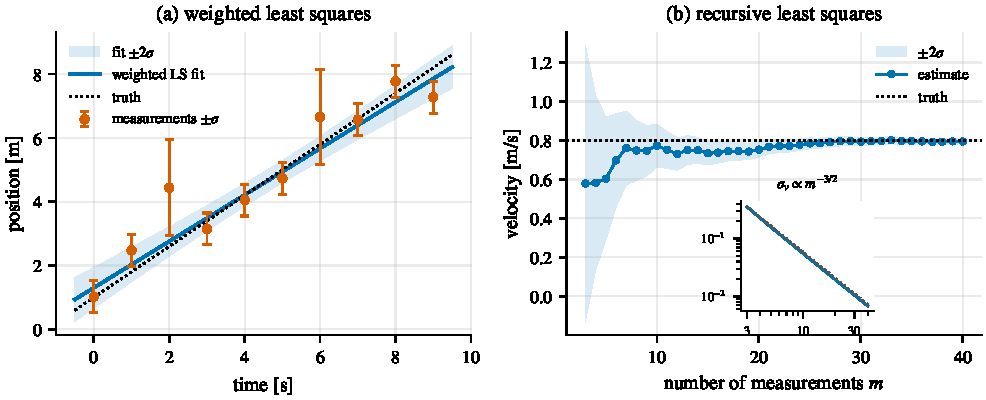
\includegraphics[width=\textwidth]{fig_lsfit.pdf}
  \caption{(a) Weighted least-squares fit of a line to noisy positions, with the $\pm2\sigma$ band of the fitted line from $(H\T R\inv H)\inv$.
  (b) Recursive least squares: the velocity estimate and its $\pm2\sigma$ bound as measurements arrive one at a time. The bound shrinks
  like $m^{-3/2}$ because later measurements also lengthen the time baseline.}
  \label{fig:lsfit}
\end{figure}

\subsection{The Gauss--Markov theorem}

Why weight by $R\inv$? Because it is the best possible linear choice.

\begin{theorem}[Gauss--Markov]
\label{thm:gauss-markov}
\index{Gauss--Markov theorem}
Among all linear unbiased estimators $\tilde x = Lz$ of $x$ in the model \eqref{eq:linear-model}, the WLS estimate \eqref{eq:wls} has the smallest
covariance: $\Cov(\tilde x) \succeq (H\T R\inv H)\inv$. It is the \term{best linear unbiased estimator} (BLUE).
\end{theorem}
\begin{proof}
Unbiasedness for every $x$ requires $LH = I$. Write $L = L_\star + D$ with $L_\star$ the WLS matrix; then $DH = 0$. The covariance is
$LRL\T = L_\star RL_\star\T + DRD\T + L_\star RD\T + DRL_\star\T$, and the cross terms vanish:
$L_\star RD\T = (H\T R\inv H)\inv H\T R\inv RD\T = (H\T R\inv H)\inv(DH)\T = 0$. So $\Cov(\tilde x) = \Cov(\hat x) + DRD\T \succeq \Cov(\hat x)$.
\end{proof}

The theorem needs no Gaussian assumption, only the first two moments of the noise. If the noise is Gaussian, more is true: WLS is the best of
\emph{all} unbiased estimators, linear or not, as the Cram\'er--Rao bound below shows.

% ==============================================================================
\section{Maximum likelihood}

\begin{definition}[Likelihood]
For a model with density $p(z\mid x)$, the \term{likelihood} of a value $x$ given observed data $z$ is $L(x) = p(z\mid x)$, viewed as a function of $x$.
The \term{maximum-likelihood} (ML) estimate maximizes it, equivalently minimizes the negative log-likelihood $-\log p(z\mid x)$.
\end{definition}

For Gaussian noise $n \sim \N(0, R)$ in $z = h(x) + n$,
\begin{equation}
  -\log p(z\mid x) = \tfrac12\big(z - h(x)\big)\T R\inv\big(z - h(x)\big) + \text{const},
\end{equation}
so ML estimation with Gaussian noise \emph{is} weighted least squares, linear or nonlinear. This is the justification of the least-squares
costs that pervade estimation, including the reprojection error of computer vision (\cref{ch:multiview}). For non-Gaussian noise, ML gives
other costs; heavy-tailed noise, for example, leads to the robust costs of \cref{ch:nlls}.

\subsection{Fisher information and the Cram\'er--Rao bound}

\begin{definition}[Fisher information]
\index{Fisher information}
For a model $p(z\mid x)$, the \term{Fisher information matrix} is
$\mathcal I(x) = \E\big[\nabla_x\log p(z\mid x)\,\nabla_x\log p(z\mid x)\T\big] = -\E\big[\nabla^2_x\log p(z\mid x)\big]$.
\end{definition}

The Fisher information measures how sharply the likelihood peaks around the true value: a likelihood that changes rapidly with $x$ pins $x$
down precisely. For the linear-Gaussian model, $\nabla^2_x\log p = -H\T R\inv H$, so $\mathcal I = H\T R\inv H$: the ``information matrix'' of WLS is the
Fisher information.

\begin{theorem}[Cram\'er--Rao lower bound]
\label{thm:crb}
\index{Cram\'er--Rao bound}
Under mild regularity conditions, every unbiased estimator satisfies $\Cov(\hat x) \succeq \mathcal I(x)\inv$.
\end{theorem}
\begin{proof}[Proof for a scalar parameter]
Let $s = \frac{\partial}{\partial x}\log p(z\mid x)$ (the \emph{score}). It has zero mean, since $\E[s] = \int\partial_xp\,\dd z = \partial_x\int p\,\dd z = 0$. Differentiating the
unbiasedness condition $\int\hat x(z)p(z\mid x)\,\dd z = x$ with respect to $x$ gives $\E[\hat x\,s] = 1$, hence $\Cov(\hat x, s) = 1$. By the
Cauchy--Schwarz inequality for covariances, $1 = \Cov(\hat x, s)^2 \le \Var(\hat x)\Var(s) = \Var(\hat x)\,\mathcal I(x)$.
\end{proof}

An unbiased estimator that attains the bound is \emph{efficient}. For the linear-Gaussian model, WLS attains it: $\Cov(\hat x) = (H\T R\inv H)\inv = \mathcal I\inv$.
No unbiased estimator can do better. This gives a precise meaning to the phrase used throughout these notes: \emph{information is inverse
covariance}, and independent measurements add their information.

% ==============================================================================
\section{Bayesian estimation}

\subsection{Priors and posteriors}

In the Bayesian view, the unknown $x$ is itself a random variable with a \emph{prior} density $p(x)$ that summarizes what is known before the
data. Bayes' rule gives the \emph{posterior} $p(x\mid z) \propto p(z\mid x)p(x)$, the complete description of what is known afterwards. Point estimates
summarize the posterior:
\begin{itemize}
  \item the \term{minimum mean-square error} (MMSE) estimate $\hat x = \E[x\mid z]$, the posterior mean;
  \item the \term{maximum a posteriori} (MAP) estimate, the posterior mode;
  \item and, ignoring the prior, the ML estimate.
\end{itemize}

\begin{theorem}[The conditional mean is optimal]
\label{thm:mmse}
Among all estimators $g(z)$, the conditional mean $\E[x\mid z]$ minimizes the Bayesian mean-square error $\E\|x - g(z)\|^2$, and indeed minimizes the
error matrix $\E[(x - g)(x - g)\T]$ in the Loewner order.
\end{theorem}
\begin{proof}
Fix $z$ and write $m = \E[x\mid z]$. For any value $g$, $\E\big[(x - g)(x - g)\T\mid z\big] = \Cov(x\mid z) + (m - g)(m - g)\T$ by the bias--variance decomposition
applied to the conditional distribution. The second term is PSD and vanishes exactly for $g = m$. Taking the expectation over $z$ preserves the
inequality.
\end{proof}

For a linear-Gaussian model the posterior is Gaussian (\cref{prop:map-ls}), so its mean and mode coincide: MMSE and MAP are the same estimate,
\begin{equation}
  \hat x = \big(P\inv + H\T R\inv H\big)\inv\big(P\inv\mu + H\T R\inv z\big), \qquad \Cov(x\mid z) = \big(P\inv + H\T R\inv H\big)\inv,
  \label{eq:bayes-linear}
\end{equation}
for a prior $\N(\mu, P)$. This is weighted least squares with one extra ``measurement'': the prior acts like a direct observation of $x$ with
value $\mu$ and covariance $P$. With an uninformative prior ($P\inv\to0$) it reduces to ML/WLS.

\subsection{Linear MMSE and the orthogonality principle}

The conditional mean can be hard to compute when distributions are not Gaussian. The best \emph{linear} (affine) estimator needs only means
and covariances.

\begin{theorem}[Linear minimum mean-square error estimator]
\label{thm:lmmse}
\index{linear MMSE estimator}\index{orthogonality principle}
Let $x$ and $z$ be random vectors with means $\mu_x$, $\mu_z$ and covariances $\Sigma_{xx}$, $\Sigma_{xz}$, $\Sigma_{zz} \succ 0$. Among estimators of the form
$\hat x = Az + b$, the mean-square error is minimized by
\begin{equation}
  \hat x = \mu_x + \Sigma_{xz}\Sigma_{zz}\inv(z - \mu_z),
  \qquad \E[(x - \hat x)(x - \hat x)\T] = \Sigma_{xx} - \Sigma_{xz}\Sigma_{zz}\inv\Sigma_{zx} .
\end{equation}
Its error is uncorrelated with the data: $\E\big[(x - \hat x)(z - \mu_z)\T\big] = 0$ (the \term{orthogonality principle}).
\end{theorem}
\begin{proof}
The error $e = x - Az - b$ has mean $\mu_x - A\mu_z - b$, which must vanish at the optimum (a non-zero mean only adds $bb\T$), so $b = \mu_x - A\mu_z$. Then
$e = (x - \mu_x) - A(z - \mu_z)$ and $\E[ee\T] = \Sigma_{xx} - A\Sigma_{zx} - \Sigma_{xz}A\T + A\Sigma_{zz}A\T$. Completing the square,
$\E[ee\T] = (A - A_\star)\Sigma_{zz}(A - A_\star)\T + \Sigma_{xx} - \Sigma_{xz}\Sigma_{zz}\inv\Sigma_{zx}$ with $A_\star = \Sigma_{xz}\Sigma_{zz}\inv$, which is minimal for $A = A_\star$. At the
optimum, $\E[e(z - \mu_z)\T] = \Sigma_{xz} - A_\star\Sigma_{zz} = 0$.
\end{proof}

The formulas are identical to Gaussian conditioning (\cref{thm:gauss-cond}): for jointly Gaussian variables the best linear estimator is the best
estimator of any kind, and for other distributions it is still the best linear one. The orthogonality principle has a geometric reading: the
estimate is the projection of $x$ onto the space of (affine) functions of the data, and the error is orthogonal to that space, exactly as a
least-squares residual is orthogonal to the column space (\cref{sec:least-squares}).

\paragraph{Application to the linear model.} For $z = Hx + n$ with prior mean $\mu$ and covariance $P$ for $x$, and noise uncorrelated with $x$:
$\mu_z = H\mu$, $\Sigma_{xz} = PH\T$, $\Sigma_{zz} = HPH\T + R$. \Cref{thm:lmmse} gives
\begin{equation}
  \hat x = \mu + K(z - H\mu), \qquad K = PH\T(HPH\T + R)\inv, \qquad \E[ee\T] = P - KHP .
  \label{eq:lmmse-update}
\end{equation}
This is the Kalman update (\cref{ch:kf}). By the Woodbury identity (\cref{thm:woodbury}) it equals \eqref{eq:bayes-linear}, but it requires
inverting an $m\times m$ matrix instead of an $n\times n$ one.

% ==============================================================================
\section{Recursive least squares}

Measurements often arrive one at a time, and recomputing \eqref{eq:wls} from scratch at each arrival would waste work. Since information adds,
the batch solution after $k$ measurements satisfies
\begin{equation}
  P_k\inv = P_{k-1}\inv + H_k\T R_k\inv H_k, \qquad P_k\inv\hat x_k = P_{k-1}\inv\hat x_{k-1} + H_k\T R_k\inv z_k,
\end{equation}
where $P_k$ is the covariance of $\hat x_k$. Rewriting this with the Woodbury identity gives the \term{recursive least squares} (RLS) update
\begin{equation}
  K_k = P_{k-1}H_k\T\big(H_kP_{k-1}H_k\T + R_k\big)\inv, \qquad
  \hat x_k = \hat x_{k-1} + K_k\big(z_k - H_k\hat x_{k-1}\big), \qquad
  P_k = (I - K_kH_k)P_{k-1} .
\end{equation}
Each step corrects the previous estimate by a gain times the \emph{innovation} $z_k - H_k\hat x_{k-1}$, the part of the new measurement that the old
estimate did not predict. It produces exactly the batch estimate at every step (\cref{fig:lsfit}b), at a cost that does not grow with the number
of measurements. RLS is the Kalman filter for a state that does not change; \cref{ch:kf} adds dynamics.

% ==============================================================================
\section{One answer, many derivations}

\begin{center}\small
\begin{tabularx}{\textwidth}{@{}l l >{\raggedright\arraybackslash}X@{}}
\toprule
Approach & Assumptions & Result for $z = Hx + n$ \\
\midrule
weighted least squares & second moments of the noise & $\hat x = (H\T R\inv H)\inv H\T R\inv z$ \\
Gauss--Markov (BLUE) & linear, unbiased & same \\
maximum likelihood & Gaussian noise & same \\
MAP / MMSE & Gaussian prior and noise & \eqref{eq:bayes-linear}: WLS with the prior as a measurement \\
linear MMSE & means and covariances only & \eqref{eq:lmmse-update}, equal to \eqref{eq:bayes-linear} \\
recursive LS & sequential data & same as batch, one measurement at a time \\
\bottomrule
\end{tabularx}
\end{center}

The Kalman filter inherits all of these interpretations. It is the exact Bayesian posterior for linear-Gaussian systems, the best linear
estimator when noises are merely uncorrelated, and a recursive least-squares solver. When models are nonlinear, these interpretations
separate, and the resulting approximations (\cref{ch:nlls,ch:nonlinear}) differ in which interpretation they try to preserve.

\begin{takeaways}
\begin{itemize}
  \item An estimator's error splits into bias and covariance: $\E[ee\T] = \Cov(\hat x) + bb\T$.
  \item Weighted least squares $\hat x = (H\T R\inv H)\inv H\T R\inv z$ has covariance $(H\T R\inv H)\inv$; information adds across independent measurements.
  \item Gauss--Markov: WLS with $R\inv$ weights is the best linear unbiased estimator.
  \item ML with Gaussian noise is least squares; the Fisher information bounds every unbiased estimator; information is inverse covariance.
  \item The conditional mean minimizes mean-square error; for Gaussians it equals the MAP estimate.
  \item The linear MMSE estimator $\mu + \Sigma_{xz}\Sigma_{zz}\inv(z - \mu_z)$ needs only second moments; its error is orthogonal to the data.
  \item Recursive least squares is the Kalman update without dynamics.
\end{itemize}
\end{takeaways}

\begin{exercises}
  \item Show that the sample mean of $m$ independent measurements of a scalar with variances $\sigma_i^2$ is not the BLUE unless all $\sigma_i$ are equal,
        and find the BLUE.
  \item For the line-fitting example with $m = 11$ measurements at $t = -5, \dots, 5$ and $\sigma = 1$, compute the covariance of $(p_0, v)$. How does it change
        if the times are $0, \dots, 10$? Interpret the off-diagonal term.
  \item Prove the matrix version of the Cram\'er--Rao bound for a linear-Gaussian model by computing $\nabla^2_x\log p$.
  \item Show that \eqref{eq:bayes-linear} and \eqref{eq:lmmse-update} agree, using \cref{thm:woodbury}.
  \item Derive the RLS update from the batch information form, and verify numerically that it reproduces the batch estimate at every step.
  \item Let $x \sim \mathcal U[-1, 1]$ and $z = x^3 + n$ with small Gaussian $n$. Compare the LMMSE estimate with the conditional mean, qualitatively. Why does
        the LMMSE estimate do poorly?
  \item A sensor reports a measurement with a bias $\beta$ that is not modeled. Show that the WLS estimate is biased by $(H\T R\inv H)\inv H\T R\inv\beta$, and explain
        why unmodeled biases are worse than large noise.
\end{exercises}
\input{chapters/solutions/09_estimation}

\chapter[Nonlinear Least Squares and Optimization]{Nonlinear Least Squares\\ and Optimization}
\label{ch:nlls}
\chaptermark{Nonlinear Least Squares} % short running header

\begin{objectives}
\begin{itemize}
  \item Formulate estimation problems with nonlinear models as nonlinear least-squares problems.
  \item Derive Newton, Gauss--Newton and Levenberg--Marquardt iterations, and understand when each converges.
  \item Optimize over manifolds such as $\SO$ by iterating in the tangent space.
  \item Make least squares robust to outliers with M-estimators and iteratively reweighted least squares.
  \item Exploit the structure of problems with poses and landmarks: the Schur complement and marginalization.
  \item See that an extended Kalman update is one Gauss--Newton step, the bridge between filtering and optimization.
\end{itemize}
\end{objectives}

Most measurement models in VIO are nonlinear: projections divide by depth, rotations enter through trigonometric functions. Maximum
likelihood with Gaussian noise then becomes a \emph{nonlinear} least-squares problem with no closed-form solution. This chapter develops the
iterative methods that solve such problems. They are used directly in this project for triangulation, and they explain what the extended
Kalman filter and the MSCKF are doing.

% ==============================================================================
\section{The problem}

Given residual functions $r_i(x)$ (measurement minus prediction) with noise covariances $R_i$, the maximum-likelihood estimate minimizes
\begin{equation}
  F(x) = \frac12\sum_i r_i(x)\T R_i\inv r_i(x) = \frac12\,r(x)\T W\,r(x),
  \label{eq:nlls}
\end{equation}
where $r$ stacks the residuals and $W = \blkdiag(R_i\inv)$. Examples in these notes:
\begin{itemize}
  \item \emph{Triangulation}: find a 3D point minimizing the reprojection errors in several images (\cref{ch:multiview}).
  \item \emph{Relative pose}: find the motion between two images that best explains point correspondences.
  \item \emph{Bundle adjustment}: find all camera poses and all points at once.
  \item \emph{Sliding-window VIO}: find a window of states minimizing visual and inertial residuals together.
\end{itemize}
Writing $W = L\T L$ (for instance $L$ the inverse of a Cholesky factor of the noise covariance) and replacing $r$ by $Lr$ \emph{whitens} the residuals,
so that $W = I$. We do this silently when convenient.

% ==============================================================================
\section{Descent methods}

The gradient and Hessian of $F$ follow from the chain rule. With $J = \partial r/\partial x$,
\begin{equation}
  \nabla F = J\T Wr, \qquad \nabla^2F = J\T WJ + \sum_k(Wr)_k\,\nabla^2r_k .
  \label{eq:nlls-derivatives}
\end{equation}

\paragraph{Gradient descent.} Step downhill, $x \gets x - \alpha\nabla F$, with a step length $\alpha$ chosen by a line search. It always makes progress for small
enough $\alpha$, but it ignores curvature and zig-zags slowly along narrow valleys.

\paragraph{Newton's method.} Minimize the quadratic Taylor model $F(x + \delta) \approx F + \nabla F\T\delta + \tfrac12\delta\T\nabla^2F\,\delta$ exactly:
\begin{equation}
  \nabla^2F\,\delta = -\nabla F .
\end{equation}
Near a minimum with positive-definite Hessian, Newton's method converges \emph{quadratically}: the number of correct digits roughly doubles each
iteration. But it needs second derivatives of every residual, and far from the minimum the Hessian may not be positive definite, in which case the
step can go uphill.

% ==============================================================================
\section{Gauss--Newton}
\label{sec:gauss-newton}

\index{Gauss--Newton method}
Least-squares problems allow a better compromise. Linearize the \emph{residuals} rather than the cost: $r(x + \delta) \approx r + J\delta$. The cost then
becomes a linear least-squares problem in $\delta$,
\begin{equation}
  \min_\delta\ \tfrac12\|r + J\delta\|_W^2
  \quad\Longrightarrow\quad
  \big(J\T WJ\big)\,\delta = -J\T Wr,
  \label{eq:gn-step}
\end{equation}
the \term{Gauss--Newton} step. Comparing with \eqref{eq:nlls-derivatives}, Gauss--Newton is Newton's method with the second term of the Hessian dropped.
That term is small when the residuals are small at the solution, or when the residuals are nearly linear, which is the common case for
well-modeled sensors. Then Gauss--Newton converges almost as fast as Newton, without second derivatives. The approximate Hessian $J\T WJ$ is
always positive semi-definite, so the step is always a descent direction (if $J$ has full column rank).

\begin{algorithm}[h]
\caption{Gauss--Newton}
\label{alg:gauss-newton}
\begin{algorithmic}[1]
\Require initial guess $x$, residual function $r(x)$ and its Jacobian $J(x)$
\Repeat
  \State evaluate $r$ and $J$ at $x$
  \State solve $(J\T WJ)\,\delta = -J\T Wr$ \Comment{Cholesky of $J\T WJ$, or QR of the whitened $J$}
  \State $x \gets x + \delta$
\Until{$\|\delta\|$ or the decrease of $F$ is below a tolerance}
\end{algorithmic}
\end{algorithm}

The linear system is the normal equation of a linear least-squares problem, so all the numerical advice of \cref{sec:least-squares} applies: for
small, well-conditioned problems Cholesky of $J\T WJ$ is fine; for ill-conditioned ones, QR of the whitened Jacobian is safer.

\paragraph{When Gauss--Newton fails.} With a poor initial guess, large residuals or strong nonlinearity, the linear model can be a bad
approximation, and a full step can increase the cost. If $J\T WJ$ is singular, some direction is not determined by the data (a \emph{gauge freedom}
or an unobservable direction), and the step is undefined.

\section{Levenberg--Marquardt}

\index{Levenberg--Marquardt method}
The \term{Levenberg--Marquardt} (LM) method damps the Gauss--Newton step:
\begin{equation}
  \big(J\T WJ + \lambda D\big)\,\delta = -J\T Wr, \qquad \lambda \ge 0,
\end{equation}
with $D = I$ or $D = \diag(J\T WJ)$. For $\lambda\to0$ it is Gauss--Newton; for large $\lambda$ the step becomes a short gradient-descent step. The damping is
adapted to how well the linear model predicted the actual change of cost. With the \emph{gain ratio}
\begin{equation}
  \rho = \frac{F(x) - F(x + \delta)}{F(x) - \tfrac12\|r + J\delta\|_W^2},
\end{equation}
a step with $\rho$ close to one is accepted and $\lambda$ decreased (trust the model more), while a step with small or negative $\rho$ is rejected and
$\lambda$ increased. LM is equivalent to a \emph{trust-region} method that restricts the step to a region where the linearization is trusted. It is
the default solver of most computer-vision and robotics libraries.

\begin{figure}[t]
  \centering
  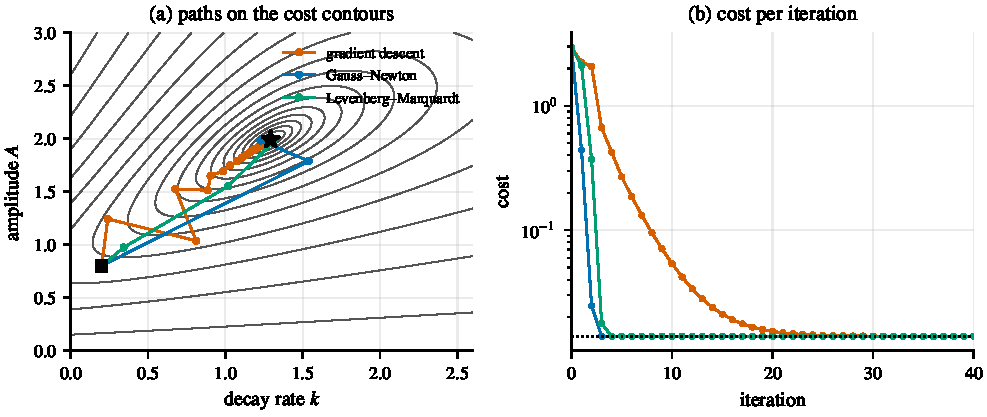
\includegraphics[width=\textwidth]{fig_gn_lm.pdf}
  \caption{Fitting the decay rate and amplitude of an exponential to noisy data. (a) Paths of gradient descent, Gauss--Newton and
  Levenberg--Marquardt on the contours of the cost, from the same starting point. (b) Cost versus iteration. Gradient descent crawls along the
  curved valley; Gauss--Newton and LM reach the minimum in a handful of iterations.}
  \label{fig:gn-lm}
\end{figure}

\section{Uncertainty of the solution}

At the minimum $\hat x$, the cost is approximately quadratic, $F(\hat x + \delta) \approx F(\hat x) + \tfrac12\delta\T(J\T WJ)\delta$, and with $W$ equal to the inverse
noise covariance the estimate has approximately the WLS covariance of the linearized problem (\cref{prop:wls-cov}):
\begin{equation}
  \Cov(\hat x) \approx \big(J\T WJ\big)\inv\Big|_{\hat x} .
\end{equation}
This is the \emph{Laplace approximation}: the posterior is replaced by a Gaussian fitted to its peak. It is accurate when the problem is nearly
linear over the region of uncertainty. A triangulated point, for example, gets a covariance from the Jacobians of its reprojection errors.

% ==============================================================================
\section{Optimization on manifolds}
\label{sec:manifold-opt}

When the unknown includes rotations, $x + \delta$ is replaced by the retraction $x\bplus\delta$ of \cref{ch:lie}. Linearize the residual in the tangent space,
$r(x\bplus\delta) \approx r(x) + J\delta$ with $J$ the manifold Jacobian (\cref{def:manifold-jacobian}), solve the same Gauss--Newton equation for $\delta$, and
update $x \gets x\bplus\delta$. The step is computed in a flat space and applied on the curved one, so the iterate never leaves the manifold and no
constraint ever needs enforcing. Covariances are then expressed in the tangent space at the solution, exactly as in a filter.

\begin{example}[Rotation averaging as Gauss--Newton]
Average rotations $R_1, \dots, R_N$ (\cref{ch:lie}) by minimizing $\tfrac12\sum_i\|r_i\|^2$ with $r_i(\bar R) = \Log(\bar R\T R_i)$. Perturbing
$\bar R\bplus\delta = \bar R\Exp(\delta)$ gives $r_i = \Log(\Exp(-\delta)\bar R\T R_i) \approx r_i(\bar R) - \Jlinv(r_i)\,\delta$ (\cref{eq:bch-left}). For small residuals
$\Jlinv \approx I$, so $J_i \approx -I$, and the Gauss--Newton step is $\delta = \frac1N\sum_ir_i$: exactly the averaging iteration of \cref{ch:lie}.
\end{example}

% ==============================================================================
\section{Robust estimation}
\label{sec:robust}

\subsection{Outliers break least squares}

A squared cost gives enormous influence to large residuals: a single wrong measurement, far from the others, can drag a least-squares estimate
arbitrarily far. Real data contain such \term{outliers}: misassociated features, reflections, moving objects. Two defenses exist: detect and
remove them (gating, RANSAC), or reduce their influence with a robust cost.

\subsection{M-estimators}

\index{M-estimator}\index{robust kernel}
An \term{M-estimator} replaces the quadratic by a function $\rho$ of the whitened residual norm $s_i = \|r_i\|_{R_i\inv}$:
\begin{equation}
  \min_x\ \sum_i\rho(s_i) .
\end{equation}

\begin{center}\small
\begin{tabular}{@{}l l l@{}}
\toprule
Kernel & $\rho(s)$ & weight $w(s) = \rho'(s)/s$ \\
\midrule
least squares & $\tfrac12s^2$ & $1$ \\
Huber & $\tfrac12s^2$ for $s\le c$;\ \ $c(s - \tfrac c2)$ otherwise & $1$ for $s \le c$;\ \ $c/s$ otherwise \\
Cauchy & $\tfrac{c^2}2\log(1 + s^2/c^2)$ & $1/(1 + s^2/c^2)$ \\
Tukey & $\tfrac{c^2}6\big(1 - (1 - s^2/c^2)^3\big)$ for $s \le c$;\ \ $c^2/6$ otherwise & $(1 - s^2/c^2)^2$ for $s \le c$;\ \ $0$ otherwise \\
\bottomrule
\end{tabular}
\end{center}

\begin{figure}[t]
  \centering
  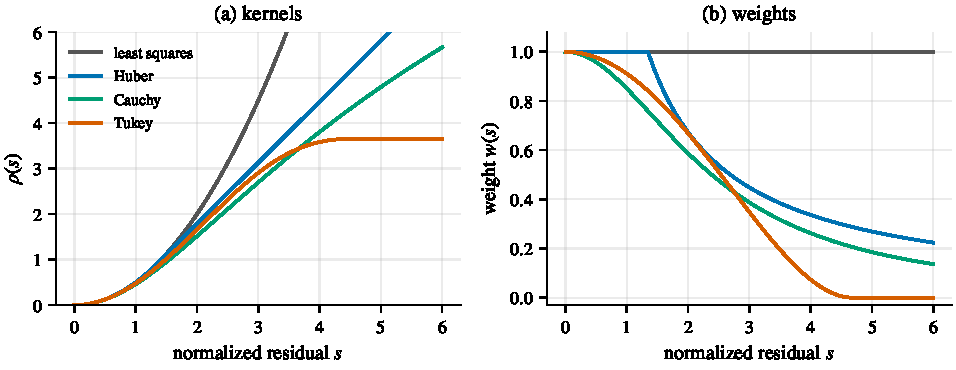
\includegraphics[width=\textwidth]{fig_robust_kernels.pdf}
  \caption{Robust kernels (left) and their weights (right) as functions of the normalized residual, for $c = 1.345$ (Huber), $2.385$ (Cauchy) and
  $4.685$ (Tukey). Huber grows linearly instead of quadratically for large residuals; Cauchy grows logarithmically; Tukey ignores residuals beyond
  $c$ entirely.}
  \label{fig:robust-kernels}
\end{figure}

The derivative $\psi = \rho'$ (the \emph{influence function}) measures how hard a residual pulls on the estimate: unbounded and linear for least squares,
bounded for Huber, decreasing to zero for Cauchy and Tukey (\cref{fig:robust-kernels}). The constants $c$ trade efficiency on clean Gaussian data against
robustness; the values in the figure keep 95\% of the efficiency of least squares on Gaussian noise.

\subsection{Iteratively reweighted least squares}

Setting the gradient of $\sum_i\rho(s_i)$ to zero gives $\sum_iw(s_i)J_i\T R_i\inv r_i = 0$ with $w(s) = \rho'(s)/s$: the normal equations of a \emph{weighted}
least-squares problem whose weights depend on the residuals. \emph{Iteratively reweighted least squares} (IRLS) alternates: compute the weights
from the current residuals, take a Gauss--Newton step with those weights, repeat. Outliers receive small weights and stop dominating. Robust
kernels need a reasonable initial guess, because with large initial errors every residual looks like an outlier; RANSAC (\cref{ch:multiview})
provides such guesses.

Gating, used in filters, is the hard-decision version of the same idea: a measurement whose normalized residual exceeds a threshold gets weight
zero, all others weight one, a ``truncated quadratic'' kernel.

% ==============================================================================
\section{Structure: poses, landmarks and the Schur complement}
\label{sec:schur-ba}

Many estimation problems have two kinds of unknowns. In bundle adjustment, the cameras $c$ and the landmarks $l$; in VIO smoothing, the states in
a window and the features. Each residual involves one camera and one landmark, so the normal equations have a special block structure:
\begin{equation}
  \begin{bmatrix} A & B \\ B\T & C \end{bmatrix}\begin{bmatrix}\delta c\\ \delta l\end{bmatrix} = \begin{bmatrix}g_c\\ g_l\end{bmatrix},
\end{equation}
where $C$, the landmark block of $J\T WJ$, is block diagonal with one $3\times3$ block per landmark (no residual involves two landmarks). Inverting $C$ is
therefore cheap. Eliminating the landmarks with the Schur complement (\cref{sec:schur}),
\begin{equation}
  \big(A - BC\inv B\T\big)\,\delta c = g_c - BC\inv g_l, \qquad \delta l = C\inv(g_l - B\T\delta c),
  \label{eq:reduced-camera-system}
\end{equation}
leaves a \emph{reduced camera system} whose size depends only on the number of cameras, often a hundred times smaller than the full problem.

\begin{figure}[t]
  \centering
  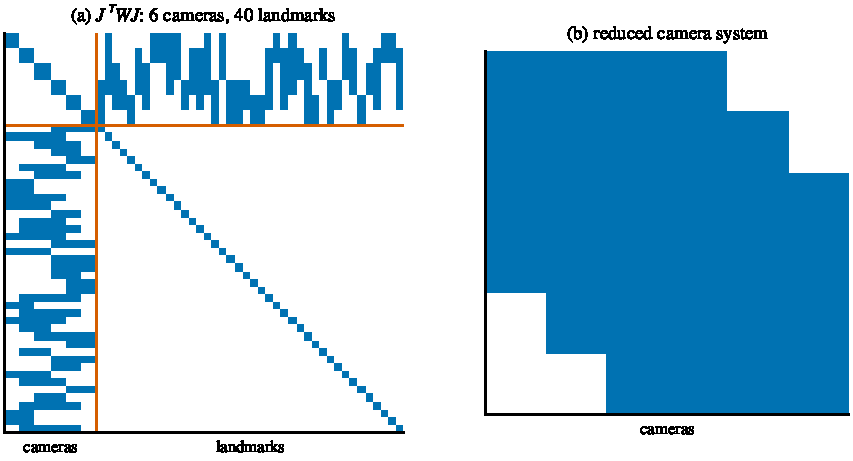
\includegraphics[width=\textwidth]{fig_ba_sparsity.pdf}
  \caption{Sparsity of the normal-equation matrix $J\T WJ$ for a toy bundle adjustment with 6 cameras and 40 landmarks (left), and of the reduced camera
  system after eliminating the landmarks (right). The landmark block is block-diagonal and cheap to eliminate; the reduced system is small but dense.}
  \label{fig:ba-sparsity}
\end{figure}

The same operation has a probabilistic meaning. $J\T WJ$ is the information matrix of the linearized problem, and the Schur complement is
\emph{marginalization in information form} (\cref{thm:gauss-cond}): the reduced system is the information that the measurements carry about the
cameras alone, after the landmarks have been integrated out. Sliding-window estimators use exactly this to discard old states, keeping their
information as a Gaussian prior on the remaining ones; the price is \emph{fill-in}, since the reduced matrix is dense (\cref{fig:ba-sparsity}). The
MSCKF performs the same elimination of each landmark, by a different algebraic route: the left-nullspace projection (\cref{ch:msckfupdate}).

% ==============================================================================
\section{Filtering as optimization}
\label{sec:filter-gn}

\begin{proposition}[The EKF update is one Gauss--Newton step]
\label{prop:ekf-gn}
\index{iterated EKF}
Consider the MAP cost of one measurement $z = h(x) + n$, $n \sim \N(0, R)$, with prior $\N(\mu, P)$:
\begin{equation*}
  F(x) = \tfrac12\|x - \mu\|^2_{P\inv} + \tfrac12\|z - h(x)\|^2_{R\inv}.
\end{equation*}
One Gauss--Newton step from $x = \mu$ gives $x^+ = \mu + K(z - h(\mu))$ with $K = PH\T(HPH\T + R)\inv$ and $H = \partial h/\partial x|_\mu$: the extended
Kalman update (\cref{ch:nonlinear}).
\end{proposition}
\begin{proof}
The stacked residual is $r(x) = \big(L_P(x - \mu),\ L_R(h(x) - z)\big)$ with $L_P\T L_P = P\inv$ and $L_R\T L_R = R\inv$. At $x = \mu$, $r = (0,\ L_R(h(\mu) - z))$ and
$J = (L_P,\ L_RH)$, so the Gauss--Newton equation \eqref{eq:gn-step} reads $(P\inv + H\T R\inv H)\delta = H\T R\inv(z - h(\mu))$. By the Woodbury identity,
$(P\inv + H\T R\inv H)\inv H\T R\inv = PH\T(HPH\T + R)\inv = K$.
\end{proof}

Iterating the Gauss--Newton step, re-linearizing $h$ at each new estimate while keeping the prior term, gives the \emph{iterated} EKF, which
handles strong measurement nonlinearities better. Sliding-window smoothers go further and re-linearize past measurements as well. The MSCKF update
is one Gauss--Newton step of a sliding-window problem whose landmarks have been eliminated (\cref{ch:msckfupdate}): filtering and optimization
are two ends of one spectrum, distinguished by how often they re-linearize and which variables they keep.

\begin{takeaways}
\begin{itemize}
  \item ML with Gaussian noise means minimizing $\tfrac12 r\T Wr$; the gradient is $J\T Wr$ and $J\T WJ$ approximates the Hessian.
  \item Gauss--Newton solves $(J\T WJ)\delta = -J\T Wr$ repeatedly; it converges fast when residuals are small or nearly linear.
  \item Levenberg--Marquardt damps the step adaptively and is robust to poor initial guesses.
  \item On manifolds, compute the step in the tangent space and apply it with $\bplus$.
  \item $(J\T WJ)\inv$ at the optimum approximates the covariance of the estimate.
  \item Robust kernels bound the influence of outliers; IRLS solves them; gating is the hard version.
  \item Eliminating landmarks with the Schur complement is marginalization in information form.
  \item An EKF update is one Gauss--Newton step on the MAP cost; iterating gives the iterated EKF.
\end{itemize}
\end{takeaways}

\begin{exercises}
  \item Derive the gradient and Hessian \eqref{eq:nlls-derivatives} of the least-squares cost.
  \item Implement Gauss--Newton and LM for fitting $y = ae^{-bt}$ to noisy data and reproduce \cref{fig:gn-lm}. Start from a poor initial guess and compare
        robustness.
  \item Show that for a zero-residual problem Gauss--Newton converges quadratically near the solution.
  \item Fit a line to data containing 20\% gross outliers with least squares, Huber IRLS and Cauchy IRLS. Compare the results.
  \item Implement the Schur-complement solution \eqref{eq:reduced-camera-system} for a random sparse problem and verify that it matches the full solve.
  \item Prove that the reduced camera system equals the inverse of the camera block of $(J\T WJ)\inv$, and interpret this as marginalization.
  \item Write out one iteration of the iterated EKF and show that it reduces to the standard EKF update after the first iteration.
\end{exercises}

\chapter{Linear Dynamical Systems}
\label{ch:linsys}

\begin{objectives}
\begin{itemize}
  \item Write physical systems in continuous- and discrete-time state-space form.
  \item Discretize deterministic inputs and white process noise exactly and approximately, including Van Loan's method.
  \item Understand stability, and why inertial errors grow polynomially.
  \item Define observability, test it with the observability matrix, and compute unobservable directions.
  \item Understand what observability means for the covariance of a Kalman filter.
\end{itemize}
\end{objectives}

The Kalman filter is built on a linear state-space model. This chapter collects the linear systems theory it needs: how to write a model, how
to turn a continuous-time model into the discrete-time form a computer processes, and how to decide whether the measurements can determine the
state at all.

% ==============================================================================
\section{State-space models}

A continuous-time linear \term{state-space model} has the form
\begin{equation}
  \dot x(t) = F(t)\,x(t) + B(t)\,u(t) + G(t)\,w(t), \qquad z(t) = H(t)\,x(t) + n(t),
  \label{eq:ct-model}
\end{equation}
with state $x$, known input $u$, white process noise $w$ (density $Q_c$), measurement $z$ and measurement noise $n$. The state is the smallest set of
numbers whose present value, together with future inputs and noises, determines the future. Its discrete-time counterpart is
\begin{equation}
  x_{k+1} = \Phi_k\,x_k + \Gamma_k\,u_k + w_k, \qquad z_k = H_k\,x_k + n_k,
  \qquad w_k \sim \N(0, Q_k),\ n_k \sim \N(0, R_k).
  \label{eq:dt-model}
\end{equation}

\begin{example}[Models used in these notes]
\label{ex:state-models}
\begin{itemize}
  \item \emph{Constant velocity}: $x = (p, v)$, $\dot p = v$, $\dot v = w$ (white acceleration). $F = \begin{bmatrix}0 & 1\\0 & 0\end{bmatrix}$, $G = \begin{bmatrix}0\\1\end{bmatrix}$.
  \item \emph{Random-walk bias}: $\dot b = w_b$. $F = 0$, $G = 1$.
  \item \emph{Inertial error model} (one axis, preview of \cref{ch:errordyn}): $\delta\dot p = \delta v$, $\delta\dot v = g\,\delta\theta - \delta b_a - n_a$,
        $\delta\dot\theta = -\delta b_g - n_g$, plus random-walk biases. A chain of integrators driven by noise.
\end{itemize}
\end{example}

The discrete-time solution follows by repeated substitution:
\begin{equation}
  x_k = \Phi(k, 0)\,x_0 + \sum_{j=0}^{k-1}\Phi(k, j+1)\big(\Gamma_ju_j + w_j\big), \qquad \Phi(k, j) = \Phi_{k-1}\Phi_{k-2}\cdots\Phi_j,
\end{equation}
the discrete analog of the variation-of-constants formula (\cref{prop:stm}).

% ==============================================================================
\section{Discretization}
\label{sec:discretization}

Physical laws are continuous, computers are discrete. Over a step $\Dt$ in which $F$, $B$ and $G$ are constant, the solution of \eqref{eq:ct-model}
(\cref{thm:lti-solution}) is
\begin{equation}
  x(t + \Dt) = \underbrace{e^{F\Dt}}_{\Phi}\,x(t) + \int_0^\Dt e^{Fs}B\,u(t + \Dt - s)\,\dd s + \underbrace{\int_0^\Dt e^{Fs}G\,w(t + \Dt - s)\,\dd s}_{w_k},
\end{equation}
which has exactly the discrete form \eqref{eq:dt-model}.

\paragraph{Deterministic inputs.} If the input is held constant over the step (a \emph{zero-order hold}, which is what a sampled IMU reading
means), the input term is $\Gamma u_k$ with $\Gamma = \int_0^\Dt e^{Fs}\,\dd s\,B$. Both $\Phi$ and $\Gamma$ come from one matrix exponential,
\begin{equation}
  \exp\!\Big(\begin{bmatrix} F & B \\ 0 & 0\end{bmatrix}\Dt\Big) = \begin{bmatrix} \Phi & \Gamma \\ 0 & I\end{bmatrix},
\end{equation}
which can be verified by noting that both sides solve the same matrix ODE in $\Dt$.

\paragraph{Process noise.} The discrete noise $w_k$ is a weighted integral of white noise, so it is zero-mean Gaussian with covariance (by the
same calculation as in \cref{prop:lyapunov})
\begin{equation}
  Q_d = \int_0^\Dt e^{Fs}\,GQ_cG\T\,e^{F\T s}\,\dd s .
  \label{eq:qd-exact}
\end{equation}

\subsection{Approximations}

Expanding to first order in $\Dt$ gives the approximations used by most real-time filters and frozen in AGENTS.md F2:
\begin{equation}
  \Phi \approx I + F\Dt, \qquad Q_d \approx GQ_cG\T\,\Dt .
  \label{eq:disc-first-order}
\end{equation}
Both are accurate to $O(\Dt^2)$ per step. The units confirm the second: a noise density $\sigma_a$ in $\mathrm{m/s^2/\sqrt{Hz}}$ gives $\sigma_a^2\Dt$ in
$\mathrm{m^2/s^2}$, a velocity variance. A second-order option adds $\tfrac12F^2\Dt^2$ to $\Phi$ and $\tfrac12(FGQ_cG\T + GQ_cG\T F\T)\Dt^2$ to $Q_d$.

\begin{example}[Double integrator]
\label{ex:double-integrator-qd}
For position and velocity driven by white acceleration of density $\sigma$, $F = \begin{bmatrix}0&1\\0&0\end{bmatrix}$, $G = \begin{bmatrix}0\\1\end{bmatrix}$, $Q_c = \sigma^2$.
\Cref{ex:double-integrator} gives $e^{Fs}G = [s;\ 1]$, so \eqref{eq:qd-exact} evaluates exactly to
\begin{equation}
  Q_d = \sigma^2\begin{bmatrix} \Dt^3/3 & \Dt^2/2 \\ \Dt^2/2 & \Dt \end{bmatrix}.
\end{equation}
The first-order approximation $Q_d \approx \diag(0, \sigma^2\Dt)$ puts no noise on position within a single step. Yet after $n$ steps of exact $\Phi$, the
accumulated position variance is $\sum_{k=1}^{n} (k\Dt)^2\sigma^2\Dt \to \sigma^2 t^3/3$ as $\Dt\to0$ (a Riemann sum), which is the exact answer of
\cref{prop:integrated-noise}. The per-step error of the approximation does not accumulate into a wrong growth law; it only introduces an $O(\Dt)$
relative error, negligible at 200~Hz.
\end{example}

\subsection{Van Loan's method}

When higher accuracy is wanted, \eqref{eq:qd-exact} can be computed exactly with a single matrix exponential~\cite{vanloan1978}.

\begin{proposition}[Van Loan]
\label{prop:vanloan}
\index{Van Loan's method}
Let $C = \exp\!\Big(\begin{bmatrix} -F & GQ_cG\T \\ 0 & F\T \end{bmatrix}\Dt\Big) = \begin{bmatrix} C_{11} & C_{12} \\ 0 & C_{22}\end{bmatrix}$. Then
$\Phi = C_{22}\T$ and $Q_d = \Phi\, C_{12}$.
\end{proposition}
\begin{proof}
For a block upper-triangular generator, the diagonal blocks of the exponential are the exponentials of the diagonal blocks, so $C_{22} = e^{F\T\Dt}$.
The off-diagonal block, as a function of $\Dt$, satisfies $\dot C_{12} = -FC_{12} + GQ_cG\T C_{22}$ with $C_{12}(0) = 0$, whose solution (variation of constants)
is $C_{12} = \int_0^\Dt e^{-F(\Dt - s)}\,GQ_cG\T\,e^{F\T s}\,\dd s$. Multiplying by $\Phi = e^{F\Dt}$ on the left, and using
$e^{F\Dt}e^{-F(\Dt - s)} = e^{Fs}$, gives $\Phi C_{12} = \int_0^\Dt e^{Fs}\,GQ_cG\T\,e^{F\T s}\,\dd s$, which is \eqref{eq:qd-exact}.
\end{proof}

For the 15-state inertial error model this costs a $30\times30$ matrix exponential per step, too expensive at 200~Hz but an excellent test oracle for the
closed forms of \cref{ch:errordyn}.

% ==============================================================================
\section{Stability}

A linear time-invariant system is \emph{stable} if its free response decays. For $\dot x = Fx$ the modes are $e^{\lambda_it}$ (\cref{thm:lti-solution}), so the
system is asymptotically stable when all eigenvalues of $F$ have negative real parts. For $x_{k+1} = \Phi x_k$ the modes are $\lambda_i^k$, so all eigenvalues of
$\Phi$ must lie strictly inside the unit circle; the two conditions correspond through $\lambda_\Phi = e^{\lambda_F\Dt}$.

Integrators have eigenvalues at zero (continuous) or one (discrete): they are \emph{marginally} stable. A single integrator holds its state; a chain of
integrators (a nilpotent $F$) makes initial errors grow \emph{polynomially}, like $t$, $t^2$, $t^3$. The error dynamics of inertial navigation are of this
kind (\cref{ex:state-models}), which is why IMU errors grow polynomially rather than exponentially, and why they never stop growing without aiding.

% ==============================================================================
\section{Observability}
\label{sec:observability-linear}

\subsection{Definition and the observability matrix}

\begin{definition}[Observability]
\index{observability}
A system is \term{observable} if the initial state $x_0$ can be determined from the inputs and the noise-free outputs over a finite time.
\end{definition}

Because the inputs are known, their contribution to the outputs can be subtracted, so observability depends only on $(\Phi, H)$. For a discrete
time-invariant system without noise, $z_k = H\Phi^kx_0$. Stacking the first $n$ outputs,
\begin{equation}
  \begin{bmatrix} z_0 \\ z_1 \\ \vdots \\ z_{n-1}\end{bmatrix} = \underbrace{\begin{bmatrix} H \\ H\Phi \\ \vdots \\ H\Phi^{n-1}\end{bmatrix}}_{\mathcal O}x_0 .
\end{equation}

\begin{theorem}[Observability rank test]
\label{thm:obs-rank}
\index{observability matrix}
The system is observable if and only if the \term{observability matrix} $\mathcal O$ has rank $n$. Its nullspace is the \term{unobservable subspace}: the
initial states that produce identically zero output forever.
\end{theorem}
\begin{proof}
If $\mathcal O$ has full column rank, $x_0$ is the unique solution of the stacked equations. If $\mathcal Ox_0 = 0$ for some $x_0 \ne 0$, then $H\Phi^kx_0 = 0$ for
$k < n$, and by the Cayley--Hamilton theorem ($\Phi^n$ is a linear combination of $I, \Phi, \dots, \Phi^{n-1}$) also for all $k \ge n$; such an $x_0$ is
indistinguishable from zero. More outputs never add rank beyond the first $n$.
\end{proof}

The unobservable subspace is invariant under $\Phi$: an unobservable error stays unobservable as the system evolves. For time-varying systems, the
same reasoning gives $\mathcal O = [H_0;\ H_1\Phi(1, 0);\ H_2\Phi(2, 0);\ \dots]$, and observability can depend on the trajectory, a fact that matters
greatly for VIO (\cref{ch:observability}).

\subsection{Examples}

\begin{example}[Position versus velocity measurements]
For the discretized constant-velocity model, $\Phi = \begin{bmatrix}1 & \Dt\\0 & 1\end{bmatrix}$.
\begin{itemize}
  \item Measuring position, $H = [1\ \ 0]$: $\mathcal O = \begin{bmatrix}1 & 0\\1 & \Dt\end{bmatrix}$ has rank 2. Velocity is observable, through the change of position.
  \item Measuring velocity, $H = [0\ \ 1]$: $\mathcal O = \begin{bmatrix}0 & 1\\0 & 1\end{bmatrix}$ has rank 1, with nullspace $(1, 0)$. Position is unobservable: shifting the whole
        trajectory changes no measurement. This is dead reckoning in one line.
\end{itemize}
\end{example}

\begin{example}[A bias that looks like the state]
Let $x = (p, b)$ with $\dot p = 0$, $\dot b = 0$ and $z = p + b$. Then $H = [1\ \ 1]$, $\Phi = I$, and $\mathcal O = \begin{bmatrix}1 & 1\\1 & 1\end{bmatrix}$ has nullspace $(1, -1)$: a
change of position compensated by an opposite change of bias is invisible. A sensor bias can be estimated only if something else breaks this
symmetry. In inertial navigation that something is motion: an accelerometer bias becomes separable from tilt once the vehicle rotates
(\cref{ch:strapdown}).
\end{example}

\begin{example}[An IMU along a line]
Let $x = (p, v, b_a)$ with $\dot p = v$, $\dot v = a_m - b_a$ ($a_m$ known) and $\dot b_a = 0$, and measure $p$. In continuous time,
$F = \begin{bmatrix}0&1&0\\0&0&-1\\0&0&0\end{bmatrix}$ and $H = [1\ 0\ 0]$, and the continuous-time observability matrix $[H;\ HF;\ HF^2]$ is
$\begin{bmatrix}1&0&0\\0&1&0\\0&0&-1\end{bmatrix}$, of full rank. Position measurements reveal velocity (one differentiation) and the accelerometer bias (two
differentiations): the reason a pose sensor makes all IMU states observable in Milestone 6.
\end{example}

\subsection{Duality and controllability}

The dual notion, \emph{controllability}, asks whether the inputs (or noises) can drive the state anywhere; its test matrix is
$[\Gamma,\ \Phi\Gamma,\ \dots,\ \Phi^{n-1}\Gamma]$, and $(\Phi, \Gamma)$ is controllable exactly when $(\Phi\T, \Gamma\T)$ is observable. For a Kalman filter,
controllability by the process noise means that every state is continually excited by noise, which keeps the filter from becoming certain
of anything and ignoring new data.

\subsection{What observability means for a filter}

For a time-invariant system that is observable from its measurements and controllable from its process noise, the Kalman filter covariance
converges to a unique, bounded steady state, whatever the initial covariance (\cref{ch:kf}). Along unobservable directions there is no such
bound: the covariance there can only grow with process noise or stay at its prior value, because no measurement reduces it. A filter must
respect this. If its linearized model makes an unobservable direction appear observable, it will \emph{reduce} the covariance along that direction
without justification, and become overconfident. This is precisely what happens to the standard EKF in VIO (\cref{ch:observability}).

\begin{takeaways}
\begin{itemize}
  \item State-space models collect everything needed to predict the future; discrete models follow from continuous ones by integrating over
        a step.
  \item $\Phi = e^{F\Dt}$, $Q_d = \int e^{Fs}GQ_cG\T e^{F\T s}\dd s$; to first order $\Phi \approx I + F\Dt$ and $Q_d \approx GQ_cG\T\Dt$. Van Loan computes both exactly.
  \item Chains of integrators are marginally stable: their errors grow polynomially.
  \item Observability: $\mathcal O = [H;\ H\Phi;\ \dots]$ must have full rank; its nullspace contains the directions the outputs cannot see.
  \item A filter may reduce uncertainty only in observable directions.
\end{itemize}
\end{takeaways}

\begin{exercises}
  \item Write the mass-spring-damper $m\ddot y + c\dot y + ky = u$ in state-space form and find its eigenvalues. When is it stable?
  \item Compute $\Gamma$ for the double integrator with a zero-order-hold acceleration input, and interpret its entries.
  \item Verify \cref{prop:vanloan} numerically for the double integrator.
  \item Find the unobservable subspace of the constant-velocity model with measurements of $p_1 - p_2$ for two independent targets.
  \item Show that the continuous-time system $\dot x = Fx$, $z = Hx$ is observable if and only if $[H;\ HF;\ \dots;\ HF^{n-1}]$ has full rank.
  \item A gyroscope measures $\omega + b_g$, and an inclinometer measures the integrated angle. Is the gyro bias observable? What if the inclinometer
        is replaced by a second gyroscope?
\end{exercises}
\input{chapters/solutions/11_linear_systems}

\chapter{The Kalman Filter}
\label{ch:kf}

\begin{objectives}
\begin{itemize}
  \item Derive the Kalman filter from Bayes' rule and Gaussian conditioning, and recognize it as linear MMSE estimation and recursive
        least squares with dynamics.
  \item Understand the gain, the innovation and its covariance, the several equivalent forms of the covariance update, and the information form.
  \item Prove that the innovations of a correct filter are white, and use this to test filters without ground truth.
  \item Know why the Joseph form is used and how to implement the update without explicit inverses.
  \item Understand steady-state behavior, sequential updates, colored noise, continuous-time filtering and smoothing.
  \item Work a filter through by hand.
\end{itemize}
\end{objectives}

Rudolf Kálmán's 1960 paper~\cite{kalman1960} gave a recursive solution to linear estimation that needs only the current estimate and covariance.
It flew on Apollo and remains the backbone of navigation. This chapter derives it for linear systems; \cref{ch:nonlinear,ch:eskf} extend it to the
nonlinear, manifold-valued state of VIO.

% ==============================================================================
\section{The model}

A discrete-time linear system with Gaussian noise is described by (\cref{ch:linsys})
\begin{align}
  x_k &= \Phi_{k}\, x_{k-1} + w_k, & w_k &\sim \N(0, Q_k), \label{eq:lin-process}\\
  z_k &= H_k\, x_k + n_k, & n_k &\sim \N(0, R_k), \label{eq:lin-meas}
\end{align}
with $x_0 \sim \N(\hat x_0, P_0)$, and with $x_0$, $\{w_k\}$ and $\{n_k\}$ mutually independent and white. $\Phi_k$ is the state transition matrix, $Q_k$ the
process noise covariance, $H_k$ the measurement matrix and $R_k$ the measurement noise covariance; known inputs add a term $\Gamma_ku_k$ that only shifts
the mean. Continuous-time models are discretized as in \cref{sec:discretization}. The goal is the posterior $p(x_k \mid z_{1:k})$ given all
measurements up to time $k$.

% ==============================================================================
\section{The Bayes filter}

Two structural assumptions make recursion possible. The state is \emph{Markov}: given $x_{k-1}$, the earlier states and measurements carry no
further information about $x_k$. And each measurement depends only on the current state. Then the posterior can be computed recursively in two
steps:
\begin{align}
  \textbf{predict:}&\quad p(x_k \mid z_{1:k-1}) = \int p(x_k \mid x_{k-1})\, p(x_{k-1}\mid z_{1:k-1})\,\dd x_{k-1}, \\
  \textbf{update:}&\quad p(x_k \mid z_{1:k}) = \frac{p(z_k \mid x_k)\, p(x_k \mid z_{1:k-1})}{p(z_k\mid z_{1:k-1})}.
\end{align}
The prediction marginalizes the previous state out of the joint density $p(x_k, x_{k-1}\mid z_{1:k-1}) = p(x_k\mid x_{k-1})p(x_{k-1}\mid z_{1:k-1})$ (using the
Markov property); the update is Bayes' rule, with the new measurement independent of the past given the current state. For a linear-Gaussian
model all of these densities are Gaussian, so each step reduces to updating a mean and a covariance. We write $\hat x_k^-$, $P_k^-$ for the predicted
(prior) moments and $\hat x_k^+$, $P_k^+$ for the updated (posterior) moments.

% ==============================================================================
\section{Derivation}

\subsection{Prediction}

By \cref{prop:affine} applied to \eqref{eq:lin-process}, with $x_{k-1}$ and $w_k$ independent,
\begin{equation}
  \hat x_k^- = \Phi_k\,\hat x_{k-1}^+, \qquad P_k^- = \Phi_k P_{k-1}^+\Phi_k\T + Q_k .
  \label{eq:kf-predict}
\end{equation}
Prediction moves the error with the dynamics and adds process noise; it never decreases uncertainty in the directions excited by $Q_k$.

\subsection{Update}

Before the measurement arrives, the state and the measurement are jointly Gaussian. From \eqref{eq:lin-meas}, dropping the time index,
\begin{equation}
  \begin{bmatrix} x \\ z \end{bmatrix} \sim \N\!\left(
    \begin{bmatrix} \hat x^- \\ H\hat x^- \end{bmatrix},
    \begin{bmatrix} P^- & P^-H\T \\ HP^- & HP^-H\T + R \end{bmatrix} \right).
\end{equation}
Conditioning on the observed $z$ with \cref{thm:gauss-cond} gives the update directly.

\begin{theorem}[Kalman update]
\label{thm:kf-update}
\index{Kalman filter!update}\index{innovation}\index{Kalman gain}
Define the \term{innovation} (residual) $r = z - H\hat x^-$, its covariance $S = HP^-H\T + R$, and the \term{Kalman gain} $K = P^-H\T S\inv$. Then
\begin{equation}
  \hat x^+ = \hat x^- + K r, \qquad P^+ = P^- - K S K\T = (I - KH)\,P^- .
  \label{eq:kf-update}
\end{equation}
\end{theorem}
\begin{proof}
\Cref{eq:gauss-cond} with $\Sigma_{ab} = P^-H\T$ and $\Sigma_{bb} = S$ gives $\hat x^+ = \hat x^- + P^-H\T S\inv(z - H\hat x^-)$ and $P^+ = P^- - P^-H\T S\inv HP^-$. Since
$KSK\T = P^-H\T S\inv HP^- = KHP^-$, both covariance forms agree.
\end{proof}

The same formulas arise from the other routes of \cref{ch:estimation}: they are the linear MMSE estimate \eqref{eq:lmmse-update} (so the Kalman filter is the
best \emph{linear} filter even for non-Gaussian noise with the same second moments), the MAP estimate of \cref{prop:map-ls}, and recursive least squares
with a prediction step inserted between measurements.

\begin{keyidea}[the gain is a ratio of uncertainties]
For a scalar state measured directly ($H = 1$), $K = \frac{P^-}{P^- + R}$ and $P^+ = \frac{P^- R}{P^- + R}$. If the prior is much more uncertain than the
sensor ($P^- \gg R$), $K \to 1$ and the estimate jumps to the measurement. If the sensor is much worse ($R \gg P^-$), $K \to 0$ and the measurement is
nearly ignored. The posterior variance is always smaller than both. In general, $K$ maps the innovation, which lives in measurement space, into a
correction in state space, including corrections to states that are not measured directly but are correlated with measured ones through
$P^-$. This is how a pose measurement corrects velocity and biases.
\end{keyidea}

\subsection{The information form}

Applying the Woodbury identity (\cref{thm:woodbury}) to $P^+ = P^- - P^-H\T(HP^-H\T + R)\inv HP^-$ gives
\begin{equation}
  (P^+)\inv = (P^-)\inv + H\T R\inv H, \qquad K = P^+ H\T R\inv .
  \label{eq:kf-info}
\end{equation}
Information adds: each independent measurement contributes $H\T R\inv H$. The covariance form \eqref{eq:kf-update} inverts an $m\times m$ matrix ($m$ =
measurement dimension); the information form inverts an $n\times n$ matrix ($n$ = state dimension). Filters use the former when $m < n$; the
\emph{information filter}, which propagates $(P\inv, P\inv\hat x)$ instead, is preferred when measurements are many and large and the prediction step is
simple.

% ==============================================================================
\section{A worked example by hand}

\begin{worked}[a random walk observed directly]
A scalar state follows $x_k = x_{k-1} + w_k$ with $Q = 1$ and is measured as $z_k = x_k + n_k$ with $R = 2$. Start from $\hat x_0 = 0$, $P_0 = 4$, and receive
$z_1 = 1.5$, $z_2 = 2.0$.
\begin{center}\small
\begin{tabular}{@{}l l l@{}}
\toprule
 & $k = 1$ & $k = 2$ \\
\midrule
predict & $\hat x_1^- = 0$, $P_1^- = 4 + 1 = 5$ & $\hat x_2^- = 1.071$, $P_2^- = 1.429 + 1 = 2.429$ \\
innovation & $r_1 = 1.5$, $S_1 = 5 + 2 = 7$ & $r_2 = 2.0 - 1.071 = 0.929$, $S_2 = 4.429$ \\
gain & $K_1 = 5/7 = 0.714$ & $K_2 = 2.429/4.429 = 0.548$ \\
update & $\hat x_1^+ = 1.071$, $P_1^+ = 5\cdot2/7 = 1.429$ & $\hat x_2^+ = 1.071 + 0.548\cdot0.929 = 1.581$, $P_2^+ = 1.097$ \\
\bottomrule
\end{tabular}
\end{center}
The variance falls from 4 to about 1.1 in two steps and then settles where the information gained per measurement balances the uncertainty added per
step: solving $P^- = P^-R/(P^- + R) + Q$ gives $P^-_\infty = \tfrac12(Q + \sqrt{Q^2 + 4QR}) = 2$, $K_\infty = 0.5$, $P^+_\infty = 1$.
\end{worked}

% ==============================================================================
\section{Properties}

\begin{proposition}[Optimality]
For the linear-Gaussian model, $\hat x_k^+ = \E[x_k\mid z_{1:k}]$: the Kalman filter is the minimum mean-square error estimator among \emph{all} estimators,
linear or not (\cref{thm:mmse}). If the noises are not Gaussian but have the stated means and covariances, it remains the best \emph{linear}
estimator (\cref{thm:lmmse}).
\end{proposition}

\begin{proposition}[Innovation properties]
\label{prop:innovation}
If the model is correct, the innovations $r_k$ are zero-mean, Gaussian, with covariance $S_k$, and uncorrelated across time. Consequently
$r_k\T S_k\inv r_k \sim \chi^2_{m_k}$.
\end{proposition}
\begin{proof}
$r_k = H_k(x_k - \hat x_k^-) + n_k$ is a linear combination of zero-mean Gaussians; its two terms are independent, giving covariance
$H_kP_k^-H_k\T + R_k = S_k$. For whiteness, take $j < k$. The innovation $r_j$ is a linear function of $z_1, \dots, z_j$. The prediction error
$x_k - \hat x_k^-$ is uncorrelated with every past measurement by the orthogonality principle (\cref{thm:lmmse}), and $n_k$ is independent of the past;
hence $\E[r_kr_j\T] = H_k\E[(x_k - \hat x_k^-)r_j\T] + \E[n_kr_j\T] = 0$. The $\chi^2$ statement is \cref{thm:mahalanobis-chi2}.
\end{proof}

\Cref{prop:innovation} is the most useful diagnostic in filtering, because it can be checked on real data without ground truth. The \term{normalized
innovation squared} (NIS) $r\T S\inv r$ should look like a $\chi^2_m$ sample, and the innovation sequence should look white. Values that are
systematically too large mean the filter is overconfident or the model is wrong; systematically too small means it is underconfident;
correlation in time reveals unmodeled dynamics. Gating (\cref{ch:updates}) uses the same statistic one measurement at a time.

\subsection{Steady state}

For a time-invariant model, the covariance recursion does not depend on the measurements at all: it can be computed in advance. Substituting the
update into the prediction gives the \emph{discrete Riccati equation}
\begin{equation}
  P_{k+1}^- = \Phi\big(P_k^- - P_k^-H\T(HP_k^-H\T + R)\inv HP_k^-\big)\Phi\T + Q .
\end{equation}
If $(\Phi, H)$ is observable (more precisely, detectable) and $(\Phi, Q^{1/2})$ is controllable (stabilizable), $P_k^-$ converges to the unique positive
semi-definite solution of the algebraic Riccati equation obtained by setting $P_{k+1}^- = P_k^-$, from any initial $P_0$, and the gain converges to a constant.
The worked example shows this convergence. Navigation filters are not time-invariant, but the same balance between injected and gained
information governs them: in observable directions the covariance settles to a level set by the noise; in unobservable directions it does not
(\cref{sec:observability-linear}).

% ==============================================================================
\section{The Joseph form}
\label{sec:joseph}

\begin{proposition}[Joseph form]
\label{prop:joseph}
\index{Joseph form}
For \emph{any} gain $K$ (optimal or not), the error covariance after the update $\hat x^+ = \hat x^- + K(z - H\hat x^-)$ is
\begin{equation}
  P^+ = (I - KH)\,P^-\,(I - KH)\T + K R K\T .
  \label{eq:joseph}
\end{equation}
For the optimal gain it equals $(I - KH)P^-$.
\end{proposition}
\begin{proof}
The posterior error is $e^+ = x - \hat x^+ = (I - KH)(x - \hat x^-) - Kn$. Its two terms are independent, so by \cref{prop:affine} its covariance is
\eqref{eq:joseph}. Expanding with $K = P^-H\T S\inv$:
$(I-KH)P^-(I-KH)\T + KRK\T = (I-KH)P^- - (I-KH)P^-H\T K\T + KRK\T = (I-KH)P^- - P^-H\T K\T + K S K\T$, and the last two terms cancel because
$KSK\T = P^-H\T K\T$.
\end{proof}

Why use the longer formula? In floating point, $(I - KH)P^-$ is the difference of two nearly equal matrices when the update is informative, and it is not
symmetric. Rounding can push small eigenvalues negative, after which the filter is broken: variances become negative, Cholesky fails, gates
misbehave. The Joseph form is a sum of a congruence of $P^-$ and a congruence of $R$, so by \cref{prop:psd} it is PSD whenever $P^-$ and $R$ are,
regardless of rounding in $K$. It also remains correct when $K$ is deliberately suboptimal (for example, a gain computed with a slightly stale $P$).
AGENTS.md F3 mandates it.

\begin{implnote}[cost of the Joseph form]
With $n$ states and $m$ measurements, $(I - KH)P(I-KH)\T$ costs $\mathcal{O}(n^3)$ if done naively. For the MSCKF ($n = 75$) this is fine. If it ever
matters, note that the update can be rearranged as $P^+ = P - KHP - (KHP)\T + K S K\T$, which costs $\mathcal{O}(n^2 m)$ and is algebraically identical to the
Joseph form for any gain. It no longer has the sum-of-congruences structure that guarantees positive semi-definiteness under rounding, though, so
keep the symmetrization and monitor the smallest eigenvalue in tests. Profile before optimizing.
\end{implnote}

% ==============================================================================
\section{Implementing the update}

\begin{algorithm}[t]
\caption{Numerically careful Kalman update}
\label{alg:kf-update}
\begin{algorithmic}[1]
\Require prior $(\hat x, P)$, measurement $z$, model $(H, R)$
\State $r \gets z - H\hat x$ \Comment{innovation}
\State $S \gets HPH\T + R$; \quad $S \gets \tfrac12(S + S\T)$
\State $L \gets \mathrm{chol}(S)$ \Comment{or LDL$^\mathsf{T}$; failure means $S$ is not PD}
\State $\gamma \gets \|L\inv r\|^2$ \Comment{NIS, for gating and logging}
\If{$\gamma > \chi^2_{0.95}(\dim r)$} \State \Return reject (and count it) \EndIf
\State solve $S\,K\T = HP$ for $K\T$ using $L$ \Comment{never form $S\inv$}
\State $\hat x \gets \hat x + Kr$
\State $P \gets (I - KH)P(I - KH)\T + KRK\T$; \quad $P \gets \tfrac12(P + P\T)$
\end{algorithmic}
\end{algorithm}

\Cref{alg:kf-update} collects the numerical rules of the previous sections. Two details deserve comment. The gain is obtained by solving
$SK\T = HP\T = HP$ (since $P$ is symmetric), so the Cholesky factor of $S$ is reused for both the gate and the gain. And symmetrization after each step
removes the asymmetry that rounding introduces, which otherwise slowly accumulates (AGENTS.md F2).

\subsection{Sequential updates}

\begin{proposition}[Sequential processing]
If a stacked measurement $z = (z_1, z_2)$ has block-diagonal noise covariance $R = \blkdiag(R_1, R_2)$, updating with $z_1$ and then with $z_2$ gives
exactly the same posterior as a single update with $z$.
\end{proposition}
\begin{proof}
With independent noise blocks, the likelihood factorizes, $p(z\mid x) = p(z_1\mid x)p(z_2\mid x)$, so
$p(x\mid z) \propto p(z_2\mid x)\,\big[p(z_1\mid x)p(x)\big] \propto p(z_2\mid x)\,p(x\mid z_1)$: updating with $z_2$ the posterior after $z_1$. Both updates are exact for linear-Gaussian
models. (In information form: the information contributions $H_1\T R_1\inv H_1 + H_2\T R_2\inv H_2$ simply add.)
\end{proof}

Sequential processing can reduce cost (several small inversions instead of one large one) and allows per-block gating. If the blocks share errors
(correlated $R$), sequential processing without accounting for the correlation is wrong. For nonlinear models the two orders differ slightly,
because the second update is linearized at the estimate produced by the first.

% ==============================================================================
\section{Extensions}

\paragraph{Colored noise.} The derivation assumed white process and measurement noise. Time-correlated disturbances are handled by adding the state of
a shaping filter to the filter state (\cref{ch:processes}): this is why IMU biases, which are random walks, are state variables.

\paragraph{Continuous time: the Kalman--Bucy filter.} For continuous measurements $z(t) = Hx + n$ with white $n$ of density $R_c$, the limit of the discrete
filter as the sampling period goes to zero is
\begin{equation}
  \dot{\hat x} = F\hat x + K\big(z - H\hat x\big), \qquad K = PH\T R_c\inv, \qquad \dot P = FP + PF\T + GQ_cG\T - PH\T R_c\inv HP,
\end{equation}
a Lyapunov equation (\cref{prop:lyapunov}) with an information term subtracted. Navigation filters process sampled measurements and use the discrete
form, but the continuous form gives insight into steady-state behavior.

\paragraph{Smoothing.} A filter estimates $x_k$ from measurements up to time $k$. A \emph{smoother} also uses later measurements, which can only improve the
estimate. The Rauch--Tung--Striebel smoother runs a Kalman filter forward, storing $\hat x_k^\pm$ and $P_k^\pm$, and then sweeps backward:
\begin{equation}
  C_k = P_k^+\Phi_{k+1}\T(P_{k+1}^-)\inv, \qquad \hat x_{k|N} = \hat x_k^+ + C_k(\hat x_{k+1|N} - \hat x_{k+1}^-), \qquad P_{k|N} = P_k^+ + C_k(P_{k+1|N} - P_{k+1}^-)C_k\T .
\end{equation}
Real-time VIO is a filtering problem, but the MSCKF smooths in a limited sense: the past poses kept as clones in its sliding window are corrected by
every later update that involves them.

% ==============================================================================
\section{A simulated example}

\begin{figure}[t]
  \centering
  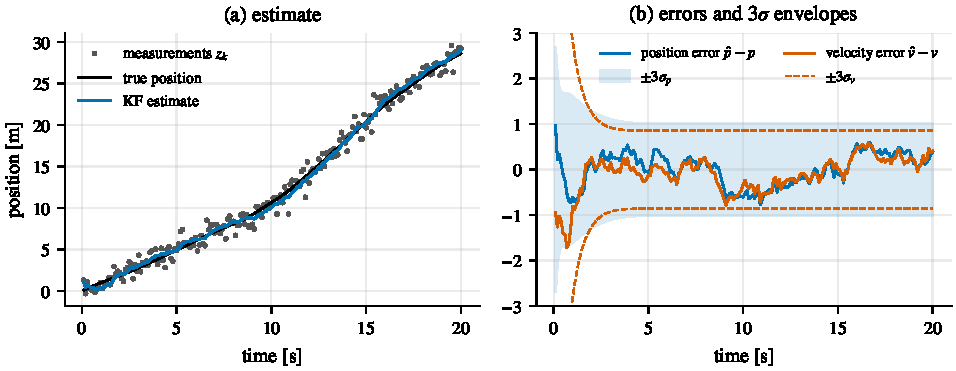
\includegraphics[width=\textwidth]{fig_kf1d.pdf}
  \caption{A constant-velocity Kalman filter tracking a 1D target from noisy position measurements. (a) The estimate smooths the measurements.
  (b) The errors stay inside the $\pm3\sigma$ envelopes, which shrink quickly from the uninformative prior and settle at the steady-state values set by
  the balance between process noise and measurement noise. The velocity is never measured, yet it is estimated through its correlation with
  position.}
  \label{fig:kf1d}
\end{figure}

\Cref{fig:kf1d} shows the filter on the constant-velocity model (\cref{ex:double-integrator-qd}), with position measurements at 10~Hz. Three behaviors
generalize to VIO. The covariance converges from its initial value to a steady state determined only by $Q$, $R$ and the geometry, not by the
data. The unmeasured state (velocity) is estimated through the correlation that the dynamics build up between position and velocity. And the errors
stay inside the $3\sigma$ envelope about 99.7\% of the time, the visual signature of a consistent filter.

\begin{takeaways}
\begin{itemize}
  \item Predict: $\hat x \gets \Phi\hat x$, $P \gets \Phi P\Phi\T + Q$. Update: condition the joint Gaussian of state and measurement.
  \item $K = PH\T S\inv$ maps innovations into state corrections, including corrections to unmeasured but correlated states.
  \item The Kalman filter is the exact Bayesian filter for linear-Gaussian models and the best linear filter otherwise.
  \item Innovations of a correct filter are white with covariance $S$; their NIS is $\chi^2$. This is testable without ground truth.
  \item Time-invariant observable systems reach a steady state set by the balance of process and measurement noise.
  \item Use the Joseph form, solve rather than invert, and symmetrize. Independent measurement blocks may be processed sequentially.
\end{itemize}
\end{takeaways}

\begin{exercises}
  \item Derive \eqref{eq:kf-update} for a scalar state measured twice by independent sensors of variances $R_1$ and $R_2$, first sequentially, then as a
        stacked 2D measurement. Show that the results agree.
  \item Show that $P^+ \preceq P^-$ for the optimal gain. Is this still true for an arbitrary gain in the Joseph form?
  \item Construct a $2\times2$ example in which $(I - KH)P^-$ computed in single precision is not positive semi-definite while the Joseph form is.
  \item Continue the worked example for five more steps and verify that $P_k^-$ converges to 2.
  \item For the scalar random walk with process variance $q$ and measurement variance $r$, derive $P^-_\infty = \tfrac12(q + \sqrt{q^2 + 4qr})$ and the
        steady-state gain. What happens as $q/r \to 0$ and $q/r \to \infty$?
  \item Implement \cref{alg:kf-update} in Python, reproduce \cref{fig:kf1d}, and compute the fraction of time steps where the position error lies outside
        $\pm3\sigma$.
  \item Test the whiteness of the innovations of your filter by computing their sample autocorrelation. Then mis-tune $Q$ and repeat.
\end{exercises}

\chapter{Nonlinear Filtering}
\label{ch:nonlinear}

\begin{objectives}
\begin{itemize}
  \item Derive the extended Kalman filter by linearization, and identify every approximation it makes.
  \item Understand the iterated EKF as Gauss--Newton.
  \item Understand the unscented transform and the unscented Kalman filter.
  \item Understand particle filters and why they do not scale to VIO.
  \item Know why VIO filters are EKFs, and what that implies for how they must be designed.
\end{itemize}
\end{objectives}

Real systems are nonlinear: rotations enter through trigonometric functions, projections divide by depth. A Gaussian pushed through a
nonlinear function is no longer Gaussian (\cref{sec:linearization}), so the exact Bayes filter of \cref{ch:kf} no longer has a finite-dimensional
form. This chapter presents the three main families of approximations. The extended Kalman filter, the basis of this project, is treated in
detail; the others are presented so that the choice is understood.

% ==============================================================================
\section{The extended Kalman filter}

\subsection{The model}

A nonlinear discrete-time model reads
\begin{equation}
  x_k = f(x_{k-1}, u_k, w_k), \qquad z_k = h(x_k) + n_k,
  \label{eq:nonlinear-model}
\end{equation}
with known input $u_k$ (an IMU reading, for instance), process noise $w_k \sim \N(0, Q_k)$ and measurement noise $n_k \sim \N(0, R_k)$.

\subsection{Derivation}

The \term{extended Kalman filter} (EKF) applies the Kalman filter to a linearization of the model about the current estimate.

\paragraph{Prediction.} Expand $f$ to first order around the previous estimate and zero noise:
\begin{equation}
  x_k \approx f(\hat x_{k-1}^+, u_k, 0) + F_k\,(x_{k-1} - \hat x_{k-1}^+) + L_kw_k,
  \qquad F_k = \frac{\partial f}{\partial x}\Big|_{\hat x_{k-1}^+},\quad L_k = \frac{\partial f}{\partial w}\Big|_{\hat x_{k-1}^+} .
\end{equation}
Taking the mean and covariance of the right-hand side (\cref{prop:affine}):
\begin{equation}
  \hat x_k^- = f(\hat x_{k-1}^+, u_k, 0), \qquad P_k^- = F_kP_{k-1}^+F_k\T + L_kQ_kL_k\T .
\end{equation}
The mean is propagated through the \emph{nonlinear} function, the covariance through its Jacobian.

\paragraph{Update.} Expand $h$ around the prediction, $h(x_k) \approx h(\hat x_k^-) + H_k(x_k - \hat x_k^-)$ with $H_k = \partial h/\partial x|_{\hat x_k^-}$, and apply the linear update with
the innovation computed from the nonlinear prediction:
\begin{equation}
\begin{gathered}
  r_k = z_k - h(\hat x_k^-), \qquad S_k = H_kP_k^-H_k\T + R_k, \qquad K_k = P_k^-H_k\T S_k\inv, \\
  \hat x_k^+ = \hat x_k^- + K_kr_k, \qquad P_k^+ = (I - K_kH_k)P_k^-(I - K_kH_k)\T + K_kR_kK_k\T .
\end{gathered}
\end{equation}

\subsection{What the EKF gets wrong}

Every step above is exact for linear models. For nonlinear models the EKF makes three approximations:
\begin{enumerate}
  \item \emph{Gaussianity}: the true prior and posterior are not Gaussian, but are represented by a mean and a covariance.
  \item \emph{Mean bias}: the predicted mean is $f(\hat x)$, not $\E[f(x)]$. By \cref{sec:linearization} the difference is about
        $\tfrac12\sum_ie_i\tr(\nabla^2f_i\,P)$, proportional to the curvature times the covariance.
  \item \emph{Covariance error}: $FPF\T$ ignores higher-order terms, and the Jacobians are evaluated at the \emph{estimate}, not at the unknown true state.
\end{enumerate}
All three errors grow with the size of the uncertainty relative to the scale over which the functions curve. When errors are small, the EKF is
excellent; when they are large, it can be badly wrong, and in particular it can become \emph{inconsistent}: report a covariance smaller than its
actual errors. The third approximation has a subtle long-term consequence in VIO, a spurious gain of information about unobservable directions
(\cref{ch:observability}).

\subsection{The iterated EKF}

By \cref{prop:ekf-gn}, the EKF update is one Gauss--Newton step on the MAP cost $\tfrac12\|x - \hat x^-\|^2_{(P^-)\inv} + \tfrac12\|z - h(x)\|^2_{R\inv}$, linearized at the prior
mean. When the measurement function is strongly nonlinear, that single step can be inaccurate. The \term{iterated EKF} (IEKF) repeats it,
re-linearizing at the latest iterate $x^{(i)}$ while keeping the prior term:
\begin{equation}
  x^{(i+1)} = \hat x^- + K^{(i)}\big(z - h(x^{(i)}) - H^{(i)}(\hat x^- - x^{(i)})\big), \qquad K^{(i)} = P^-H^{(i)\T}\big(H^{(i)}P^-H^{(i)\T} + R\big)\inv,
\end{equation}
with $H^{(i)}$ evaluated at $x^{(i)}$ and $x^{(0)} = \hat x^-$. The first iteration is the EKF. The covariance is computed with the last Jacobian. Iteration
helps when the measurement is very informative relative to the prior, so that the posterior lies far from the prior mean, where the first
linearization is poor.

% ==============================================================================
\section{Sigma-point filters}

\subsection{The unscented transform}

Linearization approximates the \emph{function}. The \term{unscented transform} approximates the \emph{distribution} instead, by a small set of
deterministically chosen \emph{sigma points} that have the right mean and covariance, and pushes each point through the exact nonlinear function.

For $x \in \R^n$ with mean $\mu$ and covariance $P = LL\T$ (Cholesky), choose $\lambda = \alpha^2(n + \kappa) - n$ and the $2n + 1$ points
\begin{equation}
  \chi_0 = \mu, \qquad \chi_i = \mu + \sqrt{n + \lambda}\,\ell_i, \qquad \chi_{n+i} = \mu - \sqrt{n + \lambda}\,\ell_i, \qquad i = 1, \dots, n,
\end{equation}
where $\ell_i$ is the $i$-th column of $L$, with weights
\begin{equation}
  W_0^{(m)} = \frac{\lambda}{n + \lambda}, \quad W_0^{(c)} = \frac{\lambda}{n + \lambda} + (1 - \alpha^2 + \beta), \quad W_i^{(m)} = W_i^{(c)} = \frac{1}{2(n + \lambda)} .
\end{equation}
Propagate $\gamma_i = f(\chi_i)$ and recombine:
\begin{equation}
  \bar y = \sum_iW_i^{(m)}\gamma_i, \qquad P_y = \sum_iW_i^{(c)}(\gamma_i - \bar y)(\gamma_i - \bar y)\T .
\end{equation}
The points are placed symmetrically along the principal axes of the uncertainty, so the weighted points reproduce $\mu$ and $P$ exactly. Expanding $f$
in a Taylor series about $\mu$ shows that $\bar y$ captures the second-order (curvature) term of the mean that linearization misses, and that
$P_y$ is correct to second order, without computing any derivatives. The parameters $\alpha$, $\beta$, $\kappa$ control the spread of the points
($\beta = 2$ is optimal for Gaussians).

\begin{figure}[t]
  \centering
  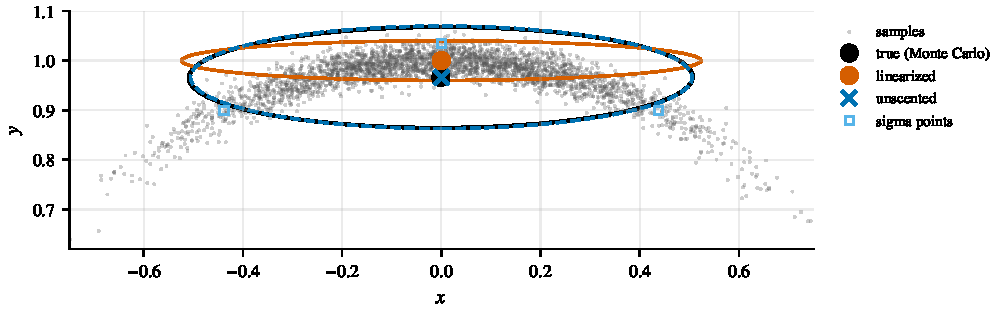
\includegraphics[width=\textwidth]{fig_ut.pdf}
  \caption{A range-bearing measurement converted to Cartesian coordinates, with $\sigma_r = 0.02$ and $\sigma_\phi = 15^\circ$. Monte Carlo samples of the true
  distribution (dots), its true mean and covariance (black), the linearized approximation (orange), and the unscented transform (blue, dashed), with the five
  sigma points; ellipses are $2\sigma$. Linearization places the mean on the circle, where it should not be; the unscented transform recovers the inward shift of the
  mean and a better covariance.}
  \label{fig:ut}
\end{figure}

\subsection{The unscented Kalman filter}

The \emph{unscented Kalman filter} (UKF) uses the unscented transform for both steps. Prediction: generate sigma points from $(\hat x^+, P^+)$, propagate them
through $f$, and recombine into $(\hat x^-, P^-)$, adding $Q$. Update: generate sigma points from $(\hat x^-, P^-)$, push them through $h$ to get the predicted
measurement $\bar z$ and its covariance $S$ (adding $R$), and the cross-covariance $P_{xz} = \sum_iW_i^{(c)}(\chi_i - \hat x^-)(\gamma_i - \bar z)\T$; then
$K = P_{xz}S\inv$, $\hat x^+ = \hat x^- + K(z - \bar z)$ and $P^+ = P^- - KSK\T$. These are the LMMSE formulas of \cref{thm:lmmse} with moments estimated by the
sigma points rather than by linearization. On manifolds, sigma points are generated in the tangent space and mapped with $\bplus$, and their mean is
computed iteratively as in \cref{ch:lie}.

The UKF costs about $2n + 1$ evaluations of $f$ and $h$ per step instead of Jacobians, which is attractive when Jacobians are hard to derive. For VIO
with a 75-dimensional state, the $151$ propagations of the full state per IMU sample are expensive, and the accuracy gain over a well-designed
error-state EKF is small, because the error-state formulation already keeps the nonlinearity mild.

% ==============================================================================
\section{Particle filters}

A \term{particle filter} represents the posterior by $N$ weighted samples (particles) $\{x^{(j)}, w^{(j)}\}$, which can represent any distribution,
multi-modal ones included. The basic \emph{sequential importance resampling} (SIR) algorithm:
\begin{enumerate}
  \item \emph{Predict}: move each particle through the dynamics with a random noise sample, $x_k^{(j)} = f(x_{k-1}^{(j)}, u_k, w^{(j)})$.
  \item \emph{Weight}: multiply each weight by the likelihood of the measurement, $w^{(j)} \gets w^{(j)}p(z_k\mid x_k^{(j)})$, and normalize.
  \item \emph{Resample}: when the effective sample size $N_{\mathrm{eff}} = 1/\sum_j(w^{(j)})^2$ falls too low, draw $N$ new particles with probabilities $w^{(j)}$ and
        reset the weights to $1/N$, so that particles concentrate where the posterior mass is.
\end{enumerate}
Particle filters are exact as $N\to\infty$ and excel at low-dimensional problems with multi-modal posteriors, such as localizing a robot in a known
map. Their weakness is dimension: the number of particles needed to cover a distribution grows roughly exponentially with the state dimension.
For the 15 to 75 dimensions of VIO they are impractical, except in hybrid forms that sample only a few variables.

% ==============================================================================
\section{Why VIO uses the EKF}

\begin{center}\small
\begin{tabularx}{\textwidth}{@{}>{\raggedright\arraybackslash}p{0.2\textwidth}>{\raggedright\arraybackslash}X>{\raggedright\arraybackslash}X>{\raggedright\arraybackslash}X@{}}
\toprule
 & EKF & UKF & particle filter \\
\midrule
cost per step & Jacobians, $\mathcal{O}(n^3)$ & $2n + 1$ propagations, $\mathcal{O}(n^3)$ & $N$ propagations, $N$ huge for large $n$ \\
derivatives needed & yes & no & no \\
non-Gaussian posteriors & no & no & yes \\
accuracy for small errors & excellent & excellent & good (noisy) \\
used in VIO & MSCKF, OpenVINS, ROVIO (iterated) & rarely & no \\
\bottomrule
\end{tabularx}
\end{center}

Visual-inertial odometry has a high-dimensional state, a fast prediction rate (hundreds of Hz), and uncertainties that, once the filter is initialized,
are small compared with the curvature of its models. Those are exactly the conditions under which the EKF is accurate and the alternatives are
expensive. The design principle that makes this work is to keep the linearized errors small: estimate the \emph{error} of a nominal state that
absorbs the large nonlinear motion, and reset it after every correction. That is the error-state Kalman filter of the next chapter.

\begin{takeaways}
\begin{itemize}
  \item The EKF propagates the mean through the nonlinear model and the covariance through its Jacobians, evaluated at the estimate.
  \item Its errors (non-Gaussianity, mean bias, covariance error, estimate-dependent Jacobians) grow with uncertainty relative to curvature.
  \item The iterated EKF is Gauss--Newton on the MAP cost; it helps when measurements are very informative.
  \item The unscented transform propagates sigma points through the exact function and captures second-order effects without derivatives.
  \item Particle filters handle any distribution but scale exponentially with dimension.
  \item VIO uses EKFs with small, frequently reset errors: the error-state formulation.
\end{itemize}
\end{takeaways}

\begin{exercises}
  \item Write the EKF for a planar robot with state $(x, y, \psi)$ driven by speed and turn rate and measured by range to a known beacon. Identify where
        linearization error enters.
  \item Reproduce \cref{fig:ut}. Increase $\sigma_\phi$ until the linearized mean lies outside the $1\sigma$ ellipse of the true distribution.
  \item Show that the unscented transform reproduces the mean and covariance exactly for a linear function.
  \item Show that for a scalar $x \sim \N(\mu, \sigma^2)$ and $f(x) = x^2$, the unscented transform with $n = 1$, $\kappa = 2$, $\alpha = 1$ gives the exact mean $\mu^2 + \sigma^2$.
  \item Implement a particle filter for a 1D robot localizing itself from range measurements to two landmarks, and observe a bimodal posterior.
\end{exercises}
\input{chapters/solutions/13_nonlinear_filtering}

\chapter{The Error-State Kalman Filter}
\label{ch:eskf}

\begin{objectives}
\begin{itemize}
  \item Understand the three-way split into true, nominal and error state, and why it is the right way to filter on a manifold.
  \item Derive the linearized error dynamics with a mechanical recipe.
  \item Define measurement residuals and Jacobians on the manifold with the correct sign convention.
  \item Derive the injection and reset steps, including the reset Jacobian $G$.
  \item Assemble the complete error-state Kalman filter loop, and follow it through a complete attitude-estimation example.
\end{itemize}
\end{objectives}

% ==============================================================================
\section{Filtering on a manifold}

The EKF of \cref{ch:nonlinear} assumes the state lives in $\R^n$, so that $\hat x + Kr$ makes sense. For VIO, the state contains a rotation, which does
not live in a vector space (\cref{ch:lie}). Three quantities must therefore be distinguished.

\begin{definition}[True, nominal and error state]
\index{error state}\index{nominal state}
\begin{itemize}
  \item The \textbf{true state} $x$ is the unknown physical state, a point on the state manifold $\mathcal{M}$.
  \item The \textbf{nominal state} $\hat x \in \mathcal{M}$ is the current best estimate, propagated with the full nonlinear model and no noise.
  \item The \textbf{error state} $\delta x = x \bminus \hat x \in \R^{n}$ is the small, minimal-dimension difference, defined with the operators of
        \cref{sec:boxplus}.
\end{itemize}
The filter's Gaussian belief is over the error state: $\delta x \sim \N(\delta\hat x, P)$, so that $x = \hat x \bplus \delta x$.
\end{definition}

For the IMU state this means 16 nominal numbers (quaternion included) but a 15-dimensional error and a $15\times15$ covariance, with no redundant
directions and no constraints. The Kalman filter operates only on the error state, which is a vector, so all of \cref{ch:kf} applies to it. This
design is called the \term{error-state Kalman filter} (ESKF), or \emph{indirect} Kalman filter. In aerospace the same idea for attitude is the
\emph{multiplicative} EKF.

\begin{keyidea}[why the error state]
\begin{itemize}
  \item \textbf{Minimal and unconstrained.} The error has exactly as many components as degrees of freedom, so its covariance is non-singular and
        needs no constraint handling.
  \item \textbf{Always near the origin.} After every update the error is reset to zero, so it never approaches the singularities of
        three-parameter rotations, and the small-angle approximations used to derive its dynamics remain valid.
  \item \textbf{Nearly linear.} The large, fast, nonlinear motion is carried by the nominal state, which is integrated exactly. The error evolves
        slowly and is small, so its dynamics are almost linear and linearization is accurate (\cref{ch:nonlinear}).
  \item \textbf{Slow.} Error dynamics are governed by sensor errors, not by vehicle motion, so the covariance could even be propagated at a lower rate
        than the nominal state if computation were scarce.
\end{itemize}
\end{keyidea}

% ==============================================================================
\section{The ESKF cycle}

\begin{figure}[t]
\centering
\begin{tikzpicture}[node distance=14mm and 30mm]
  \node[block, minimum width=40mm] (nom) {\textbf{1. Nominal propagation}\\ $\hat x \gets f(\hat x, u)$, noise-free, nonlinear};
  \node[block, minimum width=40mm, right=of nom] (cov) {\textbf{2. Covariance propagation}\\ $P \gets \Phi P\Phi\T + Q_d$};
  \node[block, minimum width=40mm, below=of cov] (upd) {\textbf{3. Update}\\ $r = z\bminus h(\hat x)$, \ $\delta\hat x = Kr$\\ $P \gets$ Joseph form};
  \node[block, minimum width=40mm, below=of nom] (inj) {\textbf{4. Inject and reset}\\ $\hat x \gets \hat x\bplus\delta\hat x$, \ $\delta\hat x \gets 0$\\ $P \gets GPG\T$};
  \draw[->, thick] (nom) -- node[note, above]{every IMU} node[note, below]{sample} (cov);
  \draw[->, thick] (cov) -- node[note, right, align=left]{measurement\\arrives} (upd);
  \draw[->, thick] (upd) -- (inj);
  \draw[->, thick] (inj) -- (nom);
  \draw[->, thick, dashed] (cov.north) to[out=135, in=45] node[note, above]{no measurement: next IMU sample} (nom.north);
\end{tikzpicture}
\caption{The error-state Kalman filter cycle. The error-state mean is zero throughout propagation, so only the covariance is propagated in step 2. It
becomes non-zero in step 3 and is transferred to the nominal state and zeroed in step 4.}
\label{fig:eskf-cycle}
\end{figure}

\Cref{fig:eskf-cycle} shows the four steps.
\begin{enumerate}
  \item \textbf{Nominal propagation.} At each IMU sample, integrate the nonlinear kinematics with the measured inputs, ignoring noise
        (\cref{ch:strapdown}).
  \item \textbf{Error covariance propagation.} Propagate $P$ with the linearized error dynamics (\cref{ch:errordyn}).
  \item \textbf{Update.} When a measurement arrives, compute the residual and its Jacobian on the manifold, and compute the Kalman estimate of the
        error, $\delta\hat x = Kr$, and the posterior covariance.
  \item \textbf{Injection and reset.} Move the estimated error into the nominal state with $\bplus$, set the error mean back to zero, and correct the
        covariance for the change of reference point.
\end{enumerate}

\begin{proposition}[The error mean needs no propagation]
If $\delta\hat x = 0$ after a reset, and the error obeys linear dynamics $\dot{\delta x} = F_c\delta x + G_cw$ with zero-mean noise, then $\E[\delta x] = 0$ until the
next update.
\end{proposition}
\begin{proof}
The mean obeys $\frac{\dd}{\dd t}\E[\delta x] = F_c\,\E[\delta x]$ (\cref{prop:lyapunov}) with initial value zero, whose unique solution is zero.
\end{proof}

This is why step 2 propagates only the covariance: all the knowledge of the error state's mean has been transferred into the nominal state.

% ==============================================================================
\section{Linearized error dynamics: the recipe}
\label{sec:error-dyn-recipe}

Suppose the true state obeys $\dot x = f(x, u, w)$ with noise $w$, and the nominal state obeys $\dot{\hat x} = f(\hat x, u, 0)$. The error dynamics are
derived in four mechanical steps.
\begin{enumerate}
  \item Write the true dynamics block by block.
  \item Substitute $x = \hat x\bplus\delta x$ in every block. For the attitude, $R = \hat R\Exp(\delta\theta)$ (or $\Exp(\delta\theta)\hat R$ for a global perturbation).
  \item Subtract the nominal dynamics.
  \item Keep only terms of first order in the small quantities ($\delta x$ and $w$), using $\Exp(\delta\theta) \approx I + \sx{\delta\theta}$ and dropping their
        products.
\end{enumerate}
The result is a linear time-varying system
\begin{equation}
  \dot{\delta x} = F_c(\hat x, u)\,\delta x + G_c(\hat x)\,w,
\end{equation}
which \cref{sec:discretization} turns into $\Phi$ and $Q_d$. The attitude block needs the time derivative of the perturbation itself, worked out in
\cref{lem:dexp}. \Cref{sec:ahrs} applies the recipe to a complete small filter, and \cref{ch:errordyn} to the inertial navigation equations.

% ==============================================================================
\section{Measurement updates on the manifold}
\label{sec:manifold-update}

Let a sensor produce a measurement $z$ on a manifold $\mathcal{Z}$ (a vector space, $\SO$, a pose, \dots) according to the generative model
\begin{equation}
  z = h(x)\bplus n, \qquad n \sim \N(0, R_z).
\end{equation}
The ESKF compares the measurement with its prediction from the nominal state,
\begin{equation}
  r = z \bminus h(\hat x),
  \label{eq:manifold-residual}
\end{equation}
and models how the residual depends on the unknown true error $\delta x$. Substituting $z = h(\hat x\bplus\delta x)\bplus n$ and linearizing,
\begin{equation}
  r \approx H\,\delta x + n, \qquad
  H = \frac{\partial}{\partial\delta x}\Big[ h(\hat x\bplus\delta x)\bminus h(\hat x) \Big]_{\delta x = 0}.
  \label{eq:manifold-H}
\end{equation}
$H$ is the manifold Jacobian of $h$ (\cref{def:manifold-jacobian}). With $r$ and $H$, the update is the ordinary Kalman update of the error state
with prior $\N(0, P)$:
\begin{equation}
  S = HPH\T + R_z,\qquad K = PH\T S\inv,\qquad \delta\hat x = Kr,\qquad P^+ = (I - KH)P(I - KH)\T + KR_zK\T.
\end{equation}

\begin{pitfall}[the sign of $H$]
There are two ways to set up the linearization, and they differ by a sign. The generative view above differentiates the \emph{prediction} with
respect to the \emph{true} error: $r \approx +H\delta x$. An optimization view instead writes the residual as a function of a correction $\delta$ to the
estimate, $e(\delta) = z\bminus h(\hat x\bplus\delta)$, whose Jacobian is $-H$ (to first order). Both lead to the same correction if used consistently.
Mixing them flips every correction. In this project, $H$ is always \eqref{eq:manifold-H}, and its finite-difference test perturbs the nominal state:
$r(\delta x) := h(\hat x\bplus\delta x)\bminus h(\hat x)$ and $H \approx \partial r/\partial\delta x$.
\end{pitfall}

For a vector-valued measurement, $\bminus$ is subtraction and this reduces to the EKF. For a rotation-valued measurement such as the pose
measurement of Milestone 6, the attitude part of the residual is $\Log_q(\hat q\inv\qprod q_{meas})$ (AGENTS.md F3).

% ==============================================================================
\section{Injection and reset}
\label{sec:reset}

After the update, the error estimate $\delta\hat x = Kr$ is non-zero. Injection moves it into the nominal state:
\begin{equation}
  \hat x^+ = \hat x\bplus\delta\hat x:\quad
  \hat p \gets \hat p + \delta\hat p,\quad \hat v \gets \hat v + \delta\hat v,\quad
  \hat q \gets \hat q\qprod\Exp_q(\delta\hat\theta),\quad \hat b \gets \hat b + \delta\hat b,
\end{equation}
followed by normalization of every quaternion that was touched, for the IMU and every clone (AGENTS.md F4).

The error is now defined relative to the new nominal state, $\delta x^+ = x\bminus\hat x^+$, and its mean is zero. But its covariance is not exactly $P^+$,
because the reference point of the tangent space has moved.

\begin{proposition}[Reset Jacobian]
\label{prop:reset}
\index{reset Jacobian}
Let $\delta x \sim \N(\delta\hat x, P^+)$ be the error relative to $\hat x$ after the update, and $\delta x^+ = x\bminus(\hat x\bplus\delta\hat x)$ the error relative to the
injected nominal state. To first order, $\delta x^+ \sim \N(0, GP^+G\T)$ with $G = \partial\delta x^+/\partial\delta x$ evaluated at $\delta\hat x$. For the vector blocks
$G = I$, and for each attitude block
\begin{equation}
  G_\theta = I - \tfrac12\sx{\delta\hat\theta}.
  \label{eq:reset-G}
\end{equation}
\end{proposition}
\begin{proof}
For vector blocks $\delta x^+ = \delta x - \delta\hat x$, whose Jacobian is $I$. For the attitude, $q = \hat q\qprod\Exp_q(\delta\theta)$ and
$q = \hat q^+\qprod\Exp_q(\delta\theta^+)$ with $\hat q^+ = \hat q\qprod\Exp_q(\delta\hat\theta)$, so
\begin{equation*}
  \Exp(\delta\theta^+) = \Exp(-\delta\hat\theta)\,\Exp(\delta\theta).
\end{equation*}
By the BCH formula \eqref{eq:bch}, $\delta\theta^+ = \delta\theta - \delta\hat\theta - \tfrac12\,\delta\hat\theta\times\delta\theta + \cdots$, whose derivative with respect to $\delta\theta$ is
$I - \tfrac12\sx{\delta\hat\theta}$. At $\delta\theta = \delta\hat\theta$ the value is exactly zero, so the new error has zero mean. Linearizing $\delta x^+$ about $\delta\hat x$ and applying
\cref{prop:affine} gives the covariance.
\end{proof}

\begin{remark}[relation to the right Jacobian]
The derivative of $\Log(\Exp(-\delta\hat\theta)\Exp(\delta\theta))$ at $\delta\theta = \delta\hat\theta$ can be computed exactly with \eqref{eq:jr-def}: it is
$\Jr(\delta\hat\theta) = I - \tfrac12\sx{\delta\hat\theta} + O(\|\delta\hat\theta\|^2)$. The frozen specification (AGENTS.md F4) uses the first-order form \eqref{eq:reset-G}. For a
typical correction of a few milliradians the two differ by about $10^{-6}$ and the difference is irrelevant. Changing it would be a logged
convention change, not a silent substitution.
\end{remark}

The covariance reset is therefore
\begin{equation}
  P \gets G P G\T, \qquad G = \blkdiag\big(I_6,\ I - \tfrac12\sx{\delta\hat\theta},\ I_6,\ \ldots\big),
\end{equation}
with one $I - \tfrac12\sx{\delta\hat\theta_i}$ block for each clone's attitude and identity elsewhere.

\begin{convention}[injection and reset, AGENTS.md F4]
Inject with $\bplus$ into the IMU block and every clone; normalize every touched quaternion; reset $\delta\hat x \gets 0$ and $P \gets GPG\T$ with $G$
implemented exactly as above. Using $G \approx I$ is a deviation that must be logged.
\end{convention}

How much does $G$ matter? It rotates the attitude covariance by half the injected correction, a first-order effect in $\|\delta\hat\theta\|$. With small
corrections at high rate the effect is tiny, and many implementations use $G = I$. Large corrections (after a long outage, or a loop closure) make it
noticeable. It costs almost nothing, and implementing it exactly removes one approximation from the consistency analysis of Milestone 7.

% ==============================================================================
\section{The complete error-state filter}

\begin{algorithm}[t]
\caption{Error-state Kalman filter (one IMU step and an optional update)}
\label{alg:eskf}
\begin{algorithmic}[1]
\Require nominal $\hat x$, covariance $P$, IMU sample at $t_k$, optional measurement $z$ at $t_k$
\State $\Dt \gets t_k - t_{k-1}$ \Comment{from integer nanosecond timestamps}
\State $\hat x \gets f(\hat x, u_k, \Dt)$; normalize $\hat q$ \Comment{nominal propagation}
\State $\Phi \gets I + F_c\Dt$; \quad $Q_d \gets G_cQ_cG_c\T\Dt$
\State $P \gets \Phi P\Phi\T + Q_d$; \quad $P \gets \tfrac12(P + P\T)$
\If{measurement $z$ available}
  \State $r \gets z\bminus h(\hat x)$; \quad $H \gets \partial[h(\hat x\bplus\delta x)\bminus h(\hat x)]/\partial\delta x$
  \State $S \gets HPH\T + R_z$; factor $S$; gate on $r\T S\inv r$
  \State $K \gets PH\T S\inv$ (by solving); \quad $\delta\hat x \gets Kr$
  \State $P \gets (I-KH)P(I-KH)\T + KR_zK\T$
  \State $\hat x \gets \hat x\bplus\delta\hat x$; normalize quaternions \Comment{inject}
  \State $P \gets GPG\T$; \quad $P \gets \tfrac12(P + P\T)$ \Comment{reset}
\EndIf
\end{algorithmic}
\end{algorithm}

\Cref{alg:eskf} assembles the pieces. It is generic: \cref{ch:strapdown,ch:errordyn} supply $f$, $F_c$ and $G_c$ for the IMU, \cref{ch:updates} supplies $h$ and $H$ for a
pose sensor, and \cref{ch:msckfupdate} supplies them for a camera. When measurements arrive between IMU samples, the filter first propagates to the
measurement time by splitting the IMU interval (\cref{ch:strapdown}).

% ==============================================================================
\section{A complete example: attitude estimation}
\label{sec:ahrs}

\index{attitude estimation}
To see every step of \cref{alg:eskf} at work on a problem small enough to follow completely, consider an \emph{attitude and heading reference system}
(AHRS) without a magnetometer: estimate the attitude $R = R_{wb}$ of a slowly moving device and the bias $b$ of its gyroscope, using the gyroscope for
propagation and the accelerometer as an inclinometer (it measures the reaction to gravity when linear accelerations are small).

To avoid solving the project's own derivation exercise, this example uses the \textbf{global} perturbation $R = \Exp(\delta\theta)\hat R$, with the error
expressed in the world frame. The project's state uses the local perturbation; its forms are the subject of the derivation exercises of \cref{ch:errordyn}\ifsolutions{}
(solutions in \cref{app:solutions})\fi.

\paragraph{State and error state.} Nominal $(\hat R, \hat b)$; error $\delta x = (\delta\theta, \delta b) \in \R^6$ with $R = \Exp(\delta\theta)\hat R$ and $b = \hat b + \delta b$.

\paragraph{Models.} Gyroscope $\omega_m = \omega + b + n_g$; bias random walk $\dot b = n_b$; accelerometer at rest $a_m = R\T v + n_a$ with $v = -g_w = (0, 0, 9.81)$.

\paragraph{Nominal propagation.} $\hat R \gets \hat R\Exp\big((\omega_m - \hat b)\Dt\big)$, $\hat b$ unchanged.

\paragraph{Error dynamics.} By \cref{ex:global-attitude} (in \cref{ch:errordyn}), $\dot{\delta\theta} = -\hat R\,\delta b - \hat R\,n_g$, and $\dot{\delta b} = n_b$. Hence
\begin{equation}
  F_c = \begin{bmatrix} 0 & -\hat R \\ 0 & 0\end{bmatrix}, \qquad G_c = \begin{bmatrix} -\hat R & 0 \\ 0 & I\end{bmatrix}, \qquad Q_c = \diag(\sigma_g^2I, \sigma_b^2I).
\end{equation}

\paragraph{Measurement Jacobian.} $h(x) = R\T v$. Perturbing, $h(\Exp(\delta\theta)\hat R) = \hat R\T\Exp(-\delta\theta)v \approx \hat R\T(v - \delta\theta\times v) = \hat R\T v + \hat R\T\sx{v}\,\delta\theta$, so
\begin{equation}
  H = \begin{bmatrix} \hat R\T\sx{v} & 0 \end{bmatrix}, \qquad r = a_m - \hat R\T v .
\end{equation}
$\sx{v}$ has rank two: the measurement observes the two components of $\delta\theta$ perpendicular to gravity (roll and pitch) but not the component along it
(yaw). It does not observe the bias directly at all.

\paragraph{Injection and reset.} $\hat R \gets \Exp(\delta\hat\theta)\hat R$, $\hat b \gets \hat b + \delta\hat b$. Repeating the reset derivation for the global perturbation,
$\Exp(\delta\theta^+) = \Exp(\delta\theta)\Exp(-\delta\hat\theta)$, gives $G_\theta = I + \tfrac12\sx{\delta\hat\theta}$: the same magnitude as \eqref{eq:reset-G}, opposite sign.

\begin{figure}[t]
  \centering
  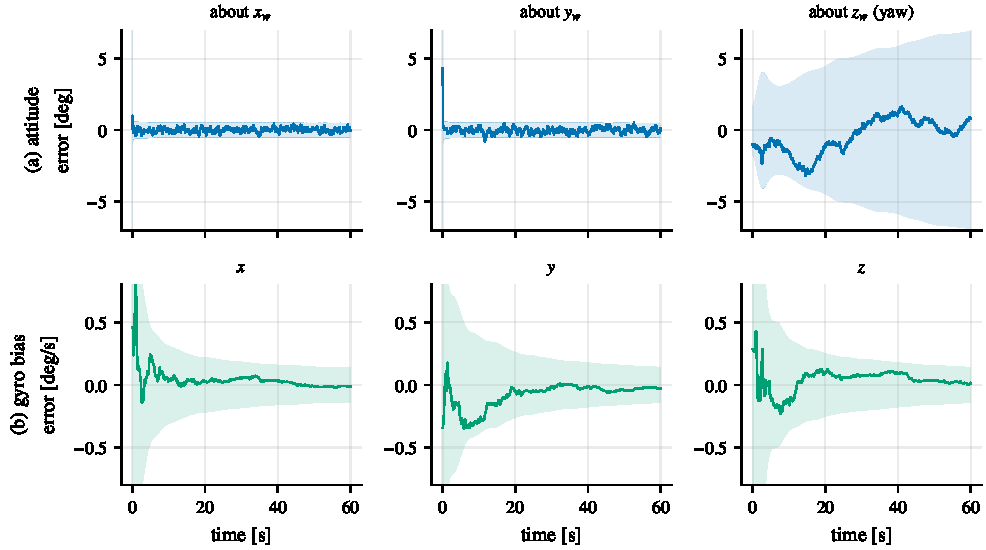
\includegraphics[width=\textwidth]{fig_ahrs.pdf}
  \caption{The attitude ESKF of \cref{sec:ahrs} on a simulated tumbling device: gyroscope at 100~Hz with a constant bias, accelerometer used as an
  inclinometer at 10~Hz. (a) Attitude errors about the world axes with their $\pm3\sigma$ bounds. Tilt (about $x$ and $y$) is quickly bounded by the
  accelerometer; the error about the vertical (yaw) is unobservable, and its bound grows. (b) Gyro bias errors with $\pm3\sigma$ bounds. The bias
  is never measured directly, yet all three components converge, because the device's rotation makes each body axis horizontal at some time.}
  \label{fig:ahrs}
\end{figure}

\Cref{fig:ahrs} shows the filter on simulated data. Several lessons of this chapter are visible in it. The errors stay inside their $3\sigma$
bounds: the filter is consistent. Tilt becomes accurate within seconds, through the accelerometer. Yaw is unobservable without a magnetometer
or vision, so its uncertainty only grows. And the gyro bias, although never measured, is estimated through its correlation with the tilt error
it causes: the cross-covariance built by propagation lets the gain correct it. This is exactly how the full VIO filter estimates IMU biases from
camera measurements.

\begin{projectlink}[Milestones 4--6]
M4 implements step 2 of \cref{alg:eskf}, M5 steps 3--4, and M6 the update, injection and reset with a pose measurement. Testing them separately
localizes bugs: if propagation is exact on synthetic data, and the covariance matches Monte Carlo statistics, then any later inconsistency is in
the update.
\end{projectlink}

\begin{takeaways}
\begin{itemize}
  \item The ESKF splits the state into a nonlinear nominal part and a small, minimal, nearly linear error part. The Kalman filter only ever sees the
        error.
  \item The error mean is zero during propagation; only $P$ is propagated.
  \item Residual $r = z\bminus h(\hat x) \approx H\delta x + n$ with $H$ the manifold Jacobian of $h$ at $\hat x$.
  \item After injection, reset $P \gets GPG\T$ with $G_\theta = I - \tfrac12\sx{\delta\hat\theta}$ for every (local) attitude block.
  \item The attitude example shows observability at work: gravity bounds tilt, yaw drifts, and unmeasured biases are estimated through
        correlations.
\end{itemize}
\end{takeaways}

\begin{exercises}
  \item Derive the reset Jacobian for the global perturbation $R = \Exp(\delta\theta)\hat R$ and confirm $G_\theta = I + \tfrac12\sx{\delta\hat\theta}$.
  \item Suppose $\delta\hat\theta = (0, 0, 0.1)$~rad and $P_{\theta\theta} = \diag(10^{-4}, 10^{-4}, 10^{-2})$. Compute $GP_{\theta\theta}G\T$ and compare with
        $\Jr(\delta\hat\theta)P_{\theta\theta}\Jr(\delta\hat\theta)\T$. When is the difference noticeable?
  \item An iterated ESKF repeats the update with $H$ re-evaluated at $\hat x\bplus\delta\hat x$. Show that one iteration is a Gauss--Newton step on the MAP cost
        $\|\delta x\|^2_{P\inv} + \|z\bminus h(\hat x\bplus\delta x)\|^2_{R_z\inv}$.
  \item Implement the attitude filter of \cref{sec:ahrs} and reproduce \cref{fig:ahrs}. Then hold the device still and observe which bias component stops
        converging. Explain why.
  \item Rewrite the attitude filter with the local perturbation $R = \hat R\Exp(\delta\theta)$: derive $F_c$, $G_c$, $H$ and $G$. (This is a small version of the project's
        derivation exercise.)
\end{exercises}
\input{chapters/solutions/14_eskf}


\part{Inertial Navigation}
\chapter{Inertial Sensors and Their Errors}
\label{ch:imu}

\begin{objectives}
\begin{itemize}
  \item Understand how MEMS accelerometers and gyroscopes work, from Newton's law and the Coriolis effect.
  \item Understand specific force: what an accelerometer measures, and why it reads $+g$ at rest.
  \item State the IMU measurement model of the project, and the fuller error model of which it is a simplification.
  \item Know how IMUs are calibrated and how their noise parameters are measured and tuned.
  \item Convert between continuous-time noise densities, discrete per-sample noise, and datasheet units.
\end{itemize}
\end{objectives}

% ==============================================================================
\section{How a MEMS accelerometer works}

A MEMS (micro-electro-mechanical system) \term{accelerometer} is a tiny proof mass, a few micrograms of silicon, suspended on silicon springs inside a
case, with capacitive electrodes that measure its displacement relative to the case.

\begin{figure}[t]
\centering
\begin{tikzpicture}[scale=1.0]
  \draw[thick] (0,0) rectangle (6,2.4);
  \node[font=\small] at (0.55,2.1) {case};
  \draw[decorate, decoration={zigzag, amplitude=2.5mm, segment length=3mm}] (0,1.2) -- (2.2,1.2);
  \node[font=\footnotesize, above] at (1.1,1.45) {spring $k$};
  \draw[fill=primarylight, draw=primary, thick] (2.2,0.7) rectangle (3.4,1.7) node[pos=0.5] {$m$};
  \draw (3.4,1.2) -- (4.2,1.2);
  \draw (4.2,0.95) -- (4.2,1.45); \draw (4.0,0.85) -- (4.6,0.85) -- (4.6,1.55) -- (4.0,1.55);
  \draw (4.6,1.2) -- (6,1.2);
  \node[font=\footnotesize, above] at (4.4,1.6) {damper $c$};
  \draw[<->, conv] (2.2,0.45) -- (2.8,0.45) node[midway, below, font=\footnotesize] {$x$};
  \draw[dashed, conv] (2.2,0.35) -- (2.2,0.75);
  \draw[->, very thick, plotorange] (6.4,1.2) -- (7.6,1.2) node[right, font=\small] {$a_{\mathrm{case}}$};
  \draw[->, thick, black!60] (3.0,-0.2) -- (3.0,-0.9) node[right, font=\small] {$g$ (along the axis if tilted)};
\end{tikzpicture}
\caption{The spring-mass-damper model of an accelerometer. The displacement $x$ of the proof mass relative to the case is proportional, at low frequencies,
to the specific force along the sensitive axis.}
\label{fig:accel-model}
\end{figure}

\subsection{The spring-mass model}

Let the case have acceleration $a$ along the sensitive axis, let $g$ be the component of gravitational acceleration along that axis, and let $x$ be the
displacement of the mass relative to the case. The absolute acceleration of the mass is $a + \ddot x$, and the forces on it are the spring, the damper
and gravity (\cref{fig:accel-model}). Newton's law gives
\begin{equation}
  m(a + \ddot x) = -kx - c\dot x + mg
  \quad\Longrightarrow\quad
  \ddot x + 2\zeta\omega_n\dot x + \omega_n^2x = -(a - g),
  \label{eq:accel-dynamics}
\end{equation}
with natural frequency $\omega_n = \sqrt{k/m}$ and damping ratio $\zeta = c/(2\sqrt{km})$. At frequencies well below $\omega_n$ the derivative terms are negligible and
\begin{equation}
  x \approx -\frac{a - g}{\omega_n^2} .
\end{equation}
The deflection measures $a - g$, not $a$. Its frequency response, the ratio of $x$ to $-(a - g)/\omega_n^2$ for a sinusoidal input at angular frequency $\omega$, is
$1/(1 - (\omega/\omega_n)^2 + 2i\zeta\omega/\omega_n)$: flat below the resonance, peaked at it for small damping, falling off above it (\cref{fig:accel-bode}).
MEMS accelerometers resonate in the kHz range, and their electronics low-pass filter the output well below that, which also serves as the
anti-aliasing filter (\cref{ch:processes}).

\begin{figure}[t]
  \centering
  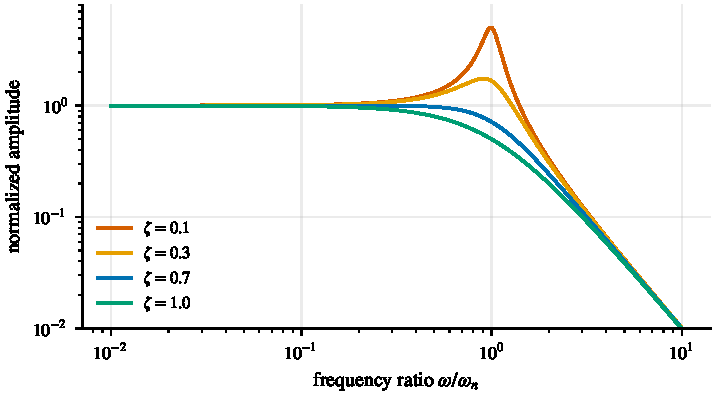
\includegraphics[width=0.84\textwidth]{fig_accel_bode.pdf}
  \caption{Frequency response of the spring-mass accelerometer model for several damping ratios. Below the natural frequency the response is flat: the
  deflection is proportional to specific force. A damping ratio near 0.7 gives the widest flat band without a resonant peak.}
  \label{fig:accel-bode}
\end{figure}

\subsection{Specific force}

\index{specific force}
The quantity measured is the \term{specific force}
\begin{equation}
  f = a - g,
\end{equation}
the non-gravitational force per unit mass acting on the sensor (the spring force divided by $m$). Gravity acts on the mass and the case equally
and cannot be felt directly: this is Einstein's equivalence principle. Two cases build intuition.
\begin{itemize}
  \item \textbf{At rest on a table}, $a = 0$, so $f = -g$. With $g_w = [0, 0, -9.81]\T$, the accelerometer reads $+9.81~\mathrm{m/s^2}$ \emph{upward}: it senses the table
        pushing it up.
  \item \textbf{In free fall}, $a = g$, so $f = 0$. A falling IMU reads zero, whatever its velocity.
\end{itemize}
To recover the kinematic acceleration from the measurement, the estimator rotates the specific force into the world frame and \emph{adds gravity back}:
$a_w = R_{wb}f_b + g_w$. A sign error here produces a vertical acceleration error of $2g \approx 20~\mathrm{m/s^2}$ and an obviously diverging altitude, which is
fortunately easy to recognize.

\paragraph{Noise.} Even a perfect mechanical sensor is noisy: the proof mass is jostled by the thermal motion of the surrounding gas, a
\emph{thermo-mechanical} noise whose acceleration density is about $\sqrt{4k_BT\omega_n/(mQ)}$ (with $k_B$ Boltzmann's constant, $T$ the temperature and $Q$ the
mechanical quality factor). Tiny masses are noisier, which is the basic trade-off of MEMS inertial sensing. Readout electronics add their own noise.

% ==============================================================================
\section{How a MEMS gyroscope works}

A MEMS \term{gyroscope} has no spinning wheel. It keeps a proof mass vibrating and detects the Coriolis force that rotation induces. Let the mass be
driven along the $x$-axis of the sensor at frequency $\omega_d$, so its velocity relative to the sensor is $v = A\omega_d\cos(\omega_dt)\,e_x$. If the sensor
rotates with angular velocity $\Omega$, then in the sensor frame the mass experiences the Coriolis acceleration $-2\Omega\times v$ (\cref{eq:coriolis}).
For a rotation about the $z$-axis this acceleration points along $y$:
\begin{equation}
  a_y = -2\,\Omega_z\,A\omega_d\cos(\omega_dt) .
\end{equation}
The resulting vibration along $y$ (the \emph{sense} mode) has an amplitude proportional to the rate $\Omega_z$ and oscillates at the drive frequency, so
the electronics recover $\Omega_z$ by demodulating the sense signal synchronously with the drive. The sensitive axis is perpendicular to both the drive and
the sense directions.

Real designs use two or four masses vibrating in anti-phase (a \emph{tuning fork}): their Coriolis forces are opposite and add in the differential
readout, while linear accelerations and vibrations push all masses the same way and cancel. Imperfect cancellation leaves a small sensitivity of the
gyro output to acceleration ($g$-sensitivity). Manufacturing asymmetries couple the drive into the sense mode (\emph{quadrature}), and their drift with
temperature is a major source of gyro bias.

% ==============================================================================
\section{The measurement model}

\subsection{The project's model}

\begin{convention}[IMU model, AGENTS.md C6]
\begin{equation}
  \omega_m = \omega_b + b_g + n_g, \qquad
  a_m = R_{wb}\T\big(a_w - g_w\big) + b_a + n_a, \qquad
  \dot b_g = n_{b_g}, \quad \dot b_a = n_{b_a},
  \label{eq:imu-model}
\end{equation}
with $\omega_m$, $a_m$ the gyroscope and accelerometer readings in the body frame, $\omega_b$ the true angular rate, $a_w$ the true acceleration of the body in the
world frame, $b_g$, $b_a$ the biases (body frame), and $n_g, n_a, n_{b_g}, n_{b_a}$ zero-mean white noises with densities $\sigma_g, \sigma_a, \sigma_{b_g}, \sigma_{b_a}$. The
noise vector is ordered $w = [n_a, n_g, n_{b_a}, n_{b_g}] \in \R^{12}$.
\end{convention}

The model has two kinds of error. \emph{White noise} ($n_g$, $n_a$) is independent from sample to sample and averages out. \emph{Bias} ($b_g$, $b_a$) is a slowly
varying offset that does not average out and is therefore estimated as part of the state (a shaping filter, \cref{ch:processes}). Its slow drift is
modeled as a random walk driven by $n_{b_g}$, $n_{b_a}$. Over the minutes of a EuRoC sequence the biases change little but measurably.

\subsection{A fuller error model}

High-accuracy inertial systems use a richer model, of which \eqref{eq:imu-model} is the special case $S = M = G = 0$:
\begin{equation}
  a_m = (I + S_a)M_a\,f_b + b_a + n_a, \qquad \omega_m = (I + S_g)M_g\,\omega_b + G_g\,f_b + b_g + n_g .
\end{equation}
Here $S$ is a diagonal matrix of \emph{scale-factor} errors (the output is $(1 + s)$ times the input), $M$ a near-identity matrix describing \emph{axis
misalignment and non-orthogonality} (the three sensing axes are neither exactly perpendicular nor exactly aligned with the body frame), and $G_g$ the
$g$-sensitivity of the gyroscope. Each of these parameters can be calibrated, estimated online as additional states, or ignored, at the cost of
some unmodeled error.

\begin{table}[t]
\centering\small
\begin{tabularx}{\textwidth}{@{}l X l@{}}
\toprule
\textbf{Error} & \textbf{Description} & \textbf{In the model?} \\
\midrule
White noise & sample-to-sample electronic and thermo-mechanical noise (angle/velocity random walk) & yes, $n_g$, $n_a$ \\
Turn-on bias & constant offset that differs at each power-up & yes, initial $b$ and $P_0$ \\
In-run bias drift & slow wandering of the offset & yes, random walk \\
Bias instability & flicker ($1/f$) noise floor of the bias & approximated by the random walk \\
Scale factor & output $= (1 + s)\times$ input & no \\
Axis misalignment & sensing axes not exactly orthogonal / aligned with the case & no \\
$g$-sensitivity & gyro output depends on acceleration & no \\
Temperature effects & bias and scale factor change with temperature & no (absorbed by bias walk) \\
Quantization & finite resolution of the ADC & no (below white noise) \\
Saturation, vibration & clipping on impacts; aliasing of high-frequency vibration & no \\
Earth rotation & gyros sense $7.3\times10^{-5}$~rad/s & no (\cref{ch:rotations}) \\
\bottomrule
\end{tabularx}
\caption{IMU error sources and how the project's model treats them.}
\label{tab:imu-errors}
\end{table}

\Cref{tab:imu-errors} lists the main error sources. Unmodeled errors do not disappear: they appear as apparent extra noise or apparent bias drift. A filter
that ignores them must compensate with larger noise parameters than the white-noise floor alone would suggest, which is why tuning is needed even with a
well-calibrated sensor. The size of the effect is easy to estimate: a scale-factor error of $10^{-3}$ on a gyro turning at 1~rad/s is an apparent bias of
$10^{-3}$~rad/s, as large as a poor bias and much larger than the EuRoC gyro's noise.

% ==============================================================================
\section{Calibration}

\paragraph{Gyroscope bias.} At rest, the gyroscope should read zero (or the Earth rate). Averaging a few seconds of data gives the bias, with a standard
deviation of $\sigma_g/\sqrt T$ after $T$ seconds (\cref{ch:processes}): for EuRoC, $10^{-4}$~rad/s after 3~s.

\paragraph{Accelerometer bias and scale: the six-position test.} Place the IMU with each axis pointing straight up and then straight down. For an axis with
bias $b$ and scale factor $1 + s$, the two readings are $(1 + s)g + b$ and $-(1 + s)g + b$, so
\begin{equation}
  b = \frac{a_{\mathrm{up}} + a_{\mathrm{down}}}{2}, \qquad 1 + s = \frac{a_{\mathrm{up}} - a_{\mathrm{down}}}{2g} .
\end{equation}
Using more orientations and a least-squares fit (\cref{ch:estimation}) also yields the misalignments.

\paragraph{Gyroscope scale and misalignment.} These require known rotations, from a rate table, or from a known sequence of orientations measured by an
accelerometer.

\paragraph{Camera--IMU calibration.} The extrinsic transform $T_{bc}$, the time offset between the sensors, and optionally the IMU's own scale and misalignment
are estimated jointly by moving the rig in front of a calibration target. The Kalibr toolbox~\cite{furgale2013kalibr}, which produced EuRoC's calibration,
represents the trajectory as a continuous-time B-spline and solves one large nonlinear least-squares problem (\cref{ch:nlls}) combining camera
reprojection errors and IMU residuals.

\paragraph{Temperature.} Biases and scale factors depend on temperature. Industrial IMUs are calibrated at several temperatures and compensated with an
on-board temperature sensor; consumer IMUs often are not, and a filter must track the resulting drift as bias random walk.

% ==============================================================================
\section{Noise parameters and their units}

The noise densities are continuous-time quantities (\cref{sec:ct-noise}). For EuRoC's ADIS16448, the \code{imu0/sensor.yaml} file gives the values in
\cref{tab:euroc-imu}.

\begin{table}[h]
\centering\small
\begin{tabular}{@{}l l l l@{}}
\toprule
YAML key & Symbol & Value & Units \\
\midrule
\code{gyroscope\_noise\_density} & $\sigma_g$ & $1.6968\times10^{-4}$ & $\mathrm{rad/s/\sqrt{Hz}}$ \\
\code{accelerometer\_noise\_density} & $\sigma_a$ & $2.0\times10^{-3}$ & $\mathrm{m/s^2/\sqrt{Hz}}$ \\
\code{gyroscope\_random\_walk} & $\sigma_{b_g}$ & $1.9393\times10^{-5}$ & $\mathrm{rad/s^2/\sqrt{Hz}}$ \\
\code{accelerometer\_random\_walk} & $\sigma_{b_a}$ & $3.0\times10^{-3}$ & $\mathrm{m/s^3/\sqrt{Hz}}$ \\
\code{rate\_hz} & $1/\Dt$ & 200 & Hz \\
\bottomrule
\end{tabular}
\caption{EuRoC IMU noise parameters (\code{imu0/sensor.yaml}). Verify against your copy of the dataset.}
\label{tab:euroc-imu}
\end{table}

The units follow from the definitions. A gyro rate in rad/s with a white noise density has units $\mathrm{rad/s}\cdot\sqrt{\mathrm{s}} = \mathrm{rad/s/\sqrt{Hz}}$. A gyro
bias random walk is the integral of white noise with units of $\mathrm{rad/s^2}$, so its density is in $\mathrm{rad/s^2/\sqrt{Hz}}$, and after $t$ seconds the
bias has standard deviation $\sigma_{b_g}\sqrt t$ in rad/s.

\paragraph{Discrete equivalents.} At sample period $\Dt$ (\cref{eq:discrete-noise}):
\begin{equation}
  \sigma_{g,d} = \frac{\sigma_g}{\sqrt\Dt}, \qquad \sigma_{a,d} = \frac{\sigma_a}{\sqrt\Dt}, \qquad
  \sigma_{b_g,d} = \sigma_{b_g}\sqrt\Dt, \qquad \sigma_{b_a,d} = \sigma_{b_a}\sqrt\Dt .
\end{equation}
For EuRoC: $\sigma_{g,d} = 2.4\times10^{-3}$~rad/s per sample, $\sigma_{a,d} = 2.8\times10^{-2}~\mathrm{m/s^2}$ per sample, and the gyro bias diffuses by
$1.4\times10^{-6}$~rad/s per sample. In the filter you never need these directly, because $Q_d = G_cQ_cG_c\T\Dt$ uses the densities, but they are what a synthetic
data generator must add to each sample.

\paragraph{Datasheet units.} Manufacturers often quote angle random walk (ARW) in $^\circ/\sqrt{\mathrm{h}}$ and velocity random walk (VRW) in $\mathrm{m/s/\sqrt{h}}$.
Since $1\ ^\circ/\sqrt{\mathrm{h}} = \frac{\pi/180}{60}~\mathrm{rad/\sqrt{s}} = 2.909\times10^{-4}~\mathrm{rad/s/\sqrt{Hz}}$, EuRoC's $\sigma_g$ is an ARW of $0.58\ ^\circ/\sqrt{\mathrm{h}}$,
and its $\sigma_a$ is a VRW of $0.12~\mathrm{m/s/\sqrt{h}}$. Bias instability is quoted in $^\circ/\mathrm{h}$ and is \emph{not} the same thing as the random walk
density.

\paragraph{Measuring them.} The densities are measured from a long static recording with the Allan variance (\cref{sec:allan,fig:allan}): white noise is read
off the slope $-\tfrac12$ at $\tau = 1$~s, and the bias random walk off the slope $+\tfrac12$ at $\tau = 3$~s.

% ==============================================================================
\section{Tuning in practice}

The densities from an Allan analysis describe a stationary sensor in a quiet lab. On a flying vehicle, vibration, temperature changes, scale-factor and
misalignment errors, timing jitter and integration error all add to the effective noise. Common practice is to start from the Allan values (or the
dataset's values) and inflate them by a modest factor until the filter is consistent, as judged by the statistical tests of \cref{ch:consistency}. Two
rules keep tuning honest.
\begin{enumerate}
  \item \textbf{Change physically meaningful parameters only}, and keep them within a plausible range of their measured values.
  \item \textbf{Judge on consistency statistics} (NEES on synthetic data, NIS and $3\sigma$ coverage on real data), not on trajectory error alone. Tuning for
        the lowest trajectory error on the test sequence is overfitting.
\end{enumerate}

\begin{pitfall}[mixing up the two discretizations]
The white-noise variance per sample is $\sigma^2/\Dt$ (larger at higher rate), while the random-walk variance per step is $\sigma_b^2\Dt$ (smaller at higher rate).
Swapping them is a common bug in synthetic data generators, and it produces noise that is wrong by a factor of $1/\Dt^2 = 40\,000$ at 200~Hz.
\end{pitfall}

\section{The EuRoC IMU stream}

EuRoC's \code{imu0/data.csv} contains one row per sample: \code{timestamp [ns], w\_x, w\_y, w\_z [rad/s], a\_x, a\_y, a\_z [m/s\textsuperscript{2}]}, i.e.\ $\omega_m$
and $a_m$ in $B$ (AGENTS.md C7). Samples arrive at nominally 200~Hz, hardware-synchronized with the cameras. The filter must nevertheless take $\Dt$ from
consecutive timestamps (AGENTS.md C5): real data has jitter and occasional gaps, which Milestone 3 logs. The ground-truth file starts later than the IMU
file, so the filter is initialized at the first ground-truth sample at or after the stream start.

\begin{projectlink}[Milestones 3 and 4]
M3 parses \code{sensor.yaml} into exactly the parameters of \cref{tab:euroc-imu} and builds the event stream. M4's synthetic trajectory generator produces
noise-free IMU data from \eqref{eq:imu-model}; adding noise with the discrete equivalents above turns it into the Monte Carlo generator of M5.
\end{projectlink}

\begin{takeaways}
\begin{itemize}
  \item An accelerometer is a spring-mass system whose deflection, below resonance, is proportional to specific force $f = a - g$: it reads $+g$ upward at rest
        and zero in free fall.
  \item A MEMS gyroscope measures the Coriolis force on a vibrating mass.
  \item $\omega_m = \omega_b + b_g + n_g$ and $a_m = R_{wb}\T(a_w - g_w) + b_a + n_a$, with random-walk biases; scale factors and misalignments are neglected.
  \item Biases and scale factors can be calibrated with static multi-position tests; camera--IMU extrinsics with a target and a continuous-time solver.
  \item Noise densities have units of $[u]/\sqrt{\mathrm{Hz}}$; per-sample white noise is $\sigma/\sqrt\Dt$, per-step bias diffusion is $\sigma_b\sqrt\Dt$.
  \item Unmodeled errors force noise inflation; tune on consistency, not on accuracy.
\end{itemize}
\end{takeaways}

\begin{exercises}
  \item An IMU lies on a table tilted by $10^\circ$ about its $x$-axis. Compute the ideal accelerometer reading. Which component reveals the tilt, and with what sign?
  \item A MEMS accelerometer has a resonance at 5~kHz. How large is its static deflection per $\mathrm{m/s^2}$? Compare with the size of a silicon atom
        ($\approx 0.2$~nm) and comment.
  \item Derive the gyroscope's Coriolis acceleration from \eqref{eq:coriolis}, and explain why a tuning-fork design rejects linear acceleration.
  \item A six-position test gives $a_{\mathrm{up}} = 9.83$ and $a_{\mathrm{down}} = -9.79~\mathrm{m/s^2}$ on one axis. Compute the bias and scale factor.
  \item A gyroscope datasheet gives ARW $= 0.2\ ^\circ/\sqrt{\mathrm{h}}$. Convert it to $\mathrm{rad/s/\sqrt{Hz}}$ and to the per-sample standard deviation at 400~Hz.
  \item A scale-factor error of $s = 10^{-3}$ affects a gyro on a vehicle spinning at 1~rad/s. What equivalent bias does it produce? Why can't a constant-bias model
        absorb it during maneuvers?
\end{exercises}

\chapter{Strapdown Propagation of the Nominal State}
\label{ch:strapdown}
\chaptermark{Strapdown Propagation} % short running header

\begin{objectives}
\begin{itemize}
  \item State the continuous-time nominal kinematics and understand each term.
  \item Derive the exact solution of the kinematics for constant inputs over a step.
  \item Compare Euler, midpoint and Runge--Kutta integration, and predict their convergence orders.
  \item Propagate to arbitrary timestamps, handle gaps, and initialize the nominal state.
  \item Understand IMU preintegration as used by optimization-based estimators.
\end{itemize}
\end{objectives}

A \emph{strapdown} inertial system has its sensors rigidly attached (strapped down) to the vehicle, as
opposed to mounted on a stabilized gimbal platform. All the work of keeping track of orientation is done in
software, by integrating the gyroscope. This chapter is about that integration.

% ------------------------------------------------------------------------------
\section{Continuous-time kinematics}

\subsection{The navigation equations}

\index{strapdown mechanization}
The \emph{mechanization equations} follow from three facts established earlier. The position changes with the velocity, $\dot p_{wb} = v_{wb}$. The
velocity changes with the acceleration, which by the definition of specific force (\cref{ch:imu}) is the measured specific force rotated into the world
frame plus gravity, $\dot v_{wb} = a_w = R_{wb}f_b + g_w$. And the attitude changes with the body angular velocity, $\dot R_{wb} = R_{wb}\sx{\omega_b}$
(\cref{sec:rot-kinematics}). Here the world frame is treated as inertial, with the effects of the Earth's rotation neglected or absorbed into gravity
and the gyro bias; \cref{ch:rotations} showed that they are tiny over the scales of a EuRoC flight. Substituting the IMU model,
$f_b = a_m - b_a - n_a$ and $\omega_b = \omega_m - b_g - n_g$, gives the true kinematics of \cref{ch:errordyn}, and replacing the unknown biases by their estimates and
setting the noise to zero gives the nominal kinematics.

\begin{convention}[nominal propagation, AGENTS.md F1]
\begin{equation}
  \hat a = a_m - \hat b_a,\quad \hat\omega = \omega_m - \hat b_g;\qquad
  \dot{\hat p} = \hat v,\quad \dot{\hat v} = \hat R_{wb}\,\hat a + g_w,\quad
  \dot{\hat q} = \tfrac12\,\hat q\qprod[0,\ \hat\omega],\quad \dot{\hat b}_a = \dot{\hat b}_g = 0 .
  \label{eq:nominal-ct}
\end{equation}
The attitude update is always multiplicative, $\hat q \gets \hat q\qprod\Exp_q(\hat\omega\Dt)$, followed by
normalization. The integration scheme for $p$ and $v$ is chosen and justified in Milestone 4 and logged
in \texttt{PROGRESS.md}.
\end{convention}

The equations form a cascade: attitude depends on the gyroscope only; velocity depends on attitude and the
accelerometer; position depends on velocity. Errors cascade the same way, which is the origin of the
$t^2$ and $t^3$ growth laws of \cref{ch:intro}.

% ------------------------------------------------------------------------------
\section{Exact solution for constant inputs}

Suppose $\hat\omega$ and $\hat a$ are constant over $[t_k, t_k + \Dt]$, which is what a zero-order hold of one
IMU sample assumes. Then the kinematics can be solved in closed form.

\begin{proposition}[Constant-input propagation]
\label{prop:exact-prop}
With $\hat\omega$, $\hat a$ constant over the step and $\phi = \hat\omega\Dt$,
\begin{align}
  \hat R_{k+1} &= \hat R_k\,\Exp(\phi), \\
  \hat v_{k+1} &= \hat v_k + g_w\Dt + \hat R_k\,\Dt\,\Jl(\phi)\,\hat a, \\
  \hat p_{k+1} &= \hat p_k + \hat v_k\Dt + \tfrac12 g_w\Dt^2 + \hat R_k\,\Dt^2\,N(\phi)\,\hat a,
\end{align}
where $N(\phi) = \sum_{j\ge0}\sx{\phi}^j/(j+2)! = \tfrac12 I + \frac{\theta - \sin\theta}{\theta^3}\sx{\phi} +
\frac{\theta^2/2 + \cos\theta - 1}{\theta^4}\sx{\phi}^2$ and $\theta = \|\phi\|$.
\end{proposition}
\begin{proof}
The attitude is \cref{prop:const-rate}. During the step $\hat R(t_k + s) = \hat R_k\Exp(\hat\omega s)$, so
$\hat v_{k+1} - \hat v_k = g_w\Dt + \hat R_k\int_0^\Dt\Exp(\hat\omega s)\,\dd s\,\hat a$, and
$\int_0^\Dt\Exp(\hat\omega s)\,\dd s = \Dt\int_0^1\Exp(u\phi)\,\dd u = \Dt\,\Jl(\phi)$ by \cref{thm:jr}. Integrating once more
gives the position, with $\int_0^\Dt\!\int_0^s\Exp(\hat\omega u)\,\dd u\,\dd s = \Dt^2N(\phi)$ by term-wise integration of
the exponential series, and the closed form follows from $\sx{\phi}^3 = -\theta^2\sx{\phi}$.
\end{proof}

For small $\phi$, $\Jl(\phi) \approx I + \tfrac12\sx{\phi}$ and $N(\phi) \approx \tfrac12 I + \tfrac16\sx{\phi}$. The
correction terms account for the rotation of the specific-force vector during the step. At 200~Hz and
1~rad/s, $\|\phi\| = 0.005$, so they change the velocity increment by about 0.25\%: small, but systematic.

% ------------------------------------------------------------------------------
\section{Numerical integration schemes}

Real inputs are not constant over a step: the IMU provides samples at $t_k$ and $t_{k+1}$, and the true signal
varies between them. Three families of schemes are common. All of them update the attitude
multiplicatively.

\paragraph{Euler with zero-order hold.} Use the sample at the start of the step for the whole step:
\begin{equation}
  \hat R_{k+1} = \hat R_k\Exp(\hat\omega_k\Dt), \quad
  \hat v_{k+1} = \hat v_k + (\hat R_k\hat a_k + g_w)\Dt, \quad
  \hat p_{k+1} = \hat p_k + \hat v_k\Dt + \tfrac12(\hat R_k\hat a_k + g_w)\Dt^2 .
\end{equation}
Local error $O(\Dt^2)$, global error $O(\Dt)$. The dominant error is essentially a \emph{half-sample time
shift}: using the sample from the start of the interval for the whole interval delays the signal by
$\Dt/2$ on average. To see the local error, expand the true velocity increment $\int_{t_k}^{t_{k+1}}a_w(t)\,\dd t = a_w(t_k)\Dt + \tfrac12\dot a_w(t_k)\Dt^2 + O(\Dt^3)$; Euler keeps
only the first term, so each step errs by $\tfrac12\dot a_w\Dt^2$, and the errors of the $T/\Dt$ steps accumulate to $O(\Dt)$.

\paragraph{Midpoint (trapezoidal).} Use the average of the two bounding samples:
\begin{equation}
  \hat R_{k+1} = \hat R_k\Exp\big(\tfrac12(\hat\omega_k + \hat\omega_{k+1})\Dt\big),\quad
  \bar a_w = \tfrac12\big(\hat R_k\hat a_k + \hat R_{k+1}\hat a_{k+1}\big) + g_w,
\end{equation}
\begin{equation*}
  \hat v_{k+1} = \hat v_k + \bar a_w\Dt, \qquad \hat p_{k+1} = \hat p_k + \hat v_k\Dt + \tfrac12\bar a_w\Dt^2 .
\end{equation*}
Local error $O(\Dt^3)$, global $O(\Dt^2)$, at the cost of having to wait for the next sample before
completing the step.

\paragraph{Runge--Kutta 4.} RK4 evaluates the dynamics at the start, twice at the middle, and at the end of
the step. Its global error is $O(\Dt^4)$ \emph{if} the inputs at mid-step are known exactly. With an IMU
they are not, and must be interpolated from the bounding samples. Linear interpolation is only
second-order accurate, which caps the whole scheme at $O(\Dt^2)$.

\begin{figure}[t]
  \centering
  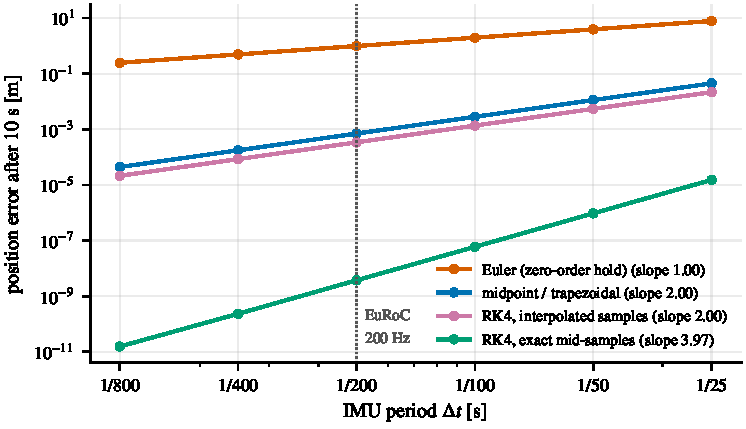
\includegraphics[width=0.86\textwidth]{fig_integration_order.pdf}
  \caption{Position error after 10~s of noise-free integration on a synthetic trajectory (2~m circle at
  0.8~rad/s with $\pm23^\circ$ roll oscillations), as a function of the IMU period. The measured slopes
  match the predicted global orders. RK4 reaches fourth order only with exact mid-step inputs, which a
  real IMU does not provide; with interpolated inputs it is no better than the midpoint rule.}
  \label{fig:integration-order}
\end{figure}

\Cref{fig:integration-order} confirms the predicted orders. Halving $\Dt$ divides the error by 2 for Euler and
by 4 for the midpoint rule, which is exactly the convergence-order test of Milestone 4. The magnitudes
matter as much as the slopes. At 200~Hz on this fairly dynamic trajectory, the Euler scheme accumulates
about a meter of error in 10~s, far more than the sensor noise would cause (\cref{fig:cov-growth}), because the
half-sample delay of the attitude creates a tilt error of order $\tfrac12\omega\Dt$, which leaks gravity. The
midpoint rule is three orders of magnitude better. On gentler motion the difference shrinks, and frequent
visual updates bound integration error in any case, but the integration error should be well below the
noise-induced error, or it becomes an unmodeled error that the filter cannot account for.

\begin{keyidea}[choosing a scheme]
The integration error is a deterministic, unmodeled error. The scheme should make it small compared with
the stochastic error the filter does model. Whichever scheme Milestone 4 adopts, document its order and
verify it with the halving test on a trajectory with closed-form ground truth.
\end{keyidea}

% ------------------------------------------------------------------------------
\section{Coning, sculling and the rotation-vector equation}
\label{sec:coning}

\subsection{The rotation vector of a step}

The attitude update over a step is a rotation $\Delta R = R(t_k)\T R(t_{k+1})$, which we can write as $\Exp(\phi)$ for a rotation vector $\phi$. If the angular
velocity keeps a fixed direction during the step, $\phi = \int\omega\,\dd t$. If its direction changes, this is wrong (\cref{prop:stm}), and the correct $\phi$
obeys a differential equation of its own.

\begin{proposition}[Bortz equation]
\label{prop:bortz}
\index{Bortz equation}
The rotation vector $\phi(t)$ with $\Exp(\phi(t)) = R(t_k)\T R(t)$ satisfies
\begin{equation}
  \dot\phi = \Jrinv(\phi)\,\omega = \omega + \tfrac12\,\phi\times\omega + D(\|\phi\|)\,\phi\times(\phi\times\omega),
\end{equation}
with $D$ the coefficient function of \cref{thm:jr}.
\end{proposition}
\begin{proof}
Over an instant $\dd t$, $\Exp(\phi + \dot\phi\,\dd t) = \Exp(\phi)\Exp(\omega\,\dd t)$. By the definition of the right Jacobian \eqref{eq:jr-def}, the left side is
$\Exp(\phi)\Exp(\Jr(\phi)\dot\phi\,\dd t)$, so $\Jr(\phi)\dot\phi = \omega$. Expand $\Jrinv$ with \eqref{eq:jrinv}.
\end{proof}

The term $\tfrac12\phi\times\omega$ is non-zero only when $\omega$ is not parallel to the rotation already accumulated: it is the \emph{non-commutativity
correction}. Under \emph{coning motion}, in which the angular velocity vector itself rotates (for example $\omega = (a\cos\Omega t,\ a\sin\Omega t,\ 0)$, the motion of
a vibrating or wobbling body), this correction does not average to zero. Integrating the rate vector alone then produces a steady, spurious
rotation about the cone axis, a drift that no amount of averaging removes.

\subsection{The two-sample coning correction}

Given the integrated gyro increments $\alpha_1$ and $\alpha_2$ over the two halves of a step (which a high-rate IMU, or two consecutive samples, provides),
the rotation vector of the whole step is, to third order,
\begin{equation}
  \phi \approx \alpha_1 + \alpha_2 + \tfrac23\,\alpha_1\times\alpha_2 .
  \label{eq:coning}
\end{equation}
\begin{proof}[Derivation]
Keep the first-order Bortz equation $\dot\phi \approx \omega + \tfrac12\phi\times\omega$ and suppose the rate varies linearly over the step, $\omega(s) = a + bs$ for
$s \in [0, h]$. To the needed order $\phi(s) \approx \int_0^s\omega = as + \tfrac12bs^2$, so
\begin{align*}
  \phi(h) &\approx \int_0^h\omega\,\dd s + \frac12\int_0^h\big(as + \tfrac12bs^2\big)\times(a + bs)\,\dd s \\
       &= \int_0^h\omega\,\dd s + \frac12(a\times b)\int_0^h\big(s^2 - \tfrac12s^2\big)\dd s
       = \alpha_1 + \alpha_2 + \frac{h^3}{12}\,a\times b .
\end{align*}
The half-step increments are $\alpha_1 = \tfrac h2a + \tfrac{h^2}8b$ and $\alpha_2 = \tfrac h2a + \tfrac{3h^2}8b$, whose cross product is $\alpha_1\times\alpha_2 = \tfrac{h^3}8\,a\times b$.
Hence $\tfrac{h^3}{12}a\times b = \tfrac23\alpha_1\times\alpha_2$.
\end{proof}

\begin{figure}[t]
  \centering
  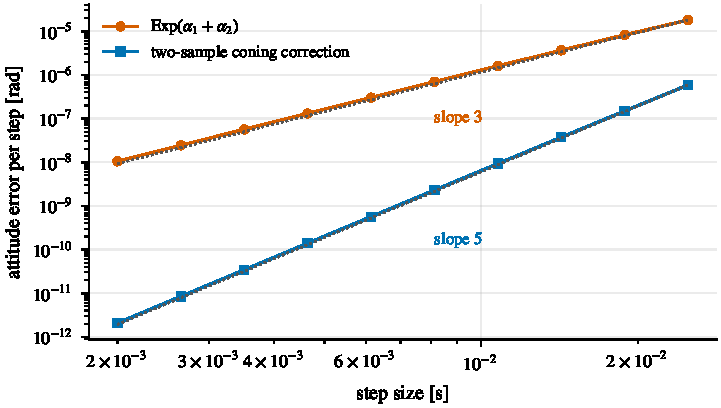
\includegraphics[width=0.84\textwidth]{fig_coning.pdf}
  \caption{Attitude error over one step under coning motion (rate amplitude 0.5~rad/s, coning frequency 10~Hz), as a function of the step size.
  Exponentiating the integrated rate errs at third order; the two-sample correction \eqref{eq:coning} reduces the error to fifth order.}
  \label{fig:coning}
\end{figure}

\Cref{fig:coning} confirms the orders. \emph{Sculling} is the analogous effect for velocity: when rotation and acceleration oscillate in phase, the
specific force is rotated while it is being integrated, and the error rectifies into a velocity drift; it has similar multi-sample corrections. High-end
inertial systems, with gyros sampled at kHz rates on vibrating platforms, rely on such algorithms~\cite{groves2013principles}. For a MEMS IMU sampled at
200~Hz, with vibration filtered by the sensor's own electronics, the effects are small compared with the sensor noise, and the project's single-sample
schemes suffice. The analysis still matters: it tells you what you are neglecting, and how to check that it is negligible.

% ------------------------------------------------------------------------------
\section{Timing}

\subsection{Propagating to an arbitrary time}

Images arrive between IMU samples. To clone the state at an image time $t_c \in (t_k, t_{k+1})$ (AGENTS.md F5), the
filter must propagate exactly to $t_c$: interpolate the IMU reading at $t_c$ linearly between samples $k$ and
$k+1$, propagate from $t_k$ to $t_c$ with the interpolated input, clone, and then propagate from $t_c$ to $t_{k+1}$.
The covariance follows the same split, with $\Dt$ replaced by the two partial intervals.

\subsection{Event ordering and gaps}

Measurements must be processed in timestamp order, and the state must be propagated to a measurement's time
before the measurement is applied (\cref{ch:fullalgo}). Milestone 3 fixes the tie rule: an IMU sample precedes a
measurement with an equal timestamp, so the state is propagated to that time first. Gaps in the IMU stream
(intervals larger than about $1.5$ nominal periods) must not be assumed away. $\Dt$ always comes from the
timestamps, and a long gap simply produces a long step with a correspondingly large $Q_d$.

% ------------------------------------------------------------------------------
\section{Initialization}

\subsection{From ground truth}

The project initializes the nominal state from the first ground-truth sample at or after the start of the
stream (Milestone 4): $p$, $v$, $q$, $b_a$ and $b_g$ all come from the ground-truth columns, mapped with the
column order of AGENTS.md C7. This isolates propagation from the initialization problem. The use of ground
truth for initialization is logged when the full VIO runs (Milestone 10b).

\subsection{Static initialization}

A real system initializes from its own sensors. If the vehicle is at rest for about a second,
\begin{equation}
  \bar a_m = \mathrm{mean}(a_m) \approx R_{wb}\T(-g_w) + b_a, \qquad \bar\omega_m = \mathrm{mean}(\omega_m) \approx b_g .
\end{equation}
The gyro bias is the mean rate. Neglecting $b_a$, the unit vector $u_b = \bar a_m/\|\bar a_m\|$ is the world
``up'' direction expressed in the body frame, $u_b = R_{wb}\T e_z$. Any rotation with $R_{wb}u_b = e_z$ is consistent
with it. One such rotation turns $u_b$ onto $e_z$ about the axis perpendicular to both:
\begin{equation}
  R_{wb} = \Exp\!\Big(\atantwo\big(\|u_b\times e_z\|,\ u_b\T e_z\big)\,\frac{u_b\times e_z}{\|u_b\times e_z\|}\Big),
\end{equation}
(with $R_{wb} = I$ if $u_b = e_z$ already), and composing it on the left with any rotation $R_z(\psi)$ about the vertical gives all the others. Roll and pitch are
determined; yaw is arbitrary, and is set to zero (or to the ground-truth yaw for evaluation).

\begin{pitfall}[tilt and accelerometer bias are indistinguishable at rest]
A horizontal accelerometer bias $b_a$ produces the same reading as a tilt of $\|b_a\|/g$: a bias of
$10~\mathrm{mm/s^2}$ looks exactly like a tilt of $1$~mrad. At rest the filter cannot separate them, and the initial
covariance must say so (large $\sigma_{b_a}$, correlated with the tilt). They become separable once the vehicle
rotates, because the bias rotates with the body while gravity does not.
\end{pitfall}

Initial covariances should reflect real uncertainty: a few milliradians in roll and pitch, a large or
unknown yaw, the turn-on bias range from the datasheet, and a small but non-zero velocity uncertainty at rest.
\emph{Dynamic} initialization from a moving start, as in VINS-Mono~\cite{qin2018vins}, first solves a
vision-only structure-from-motion problem and then aligns it with preintegrated IMU data to recover scale,
gravity and velocity.

% ------------------------------------------------------------------------------
\section{Sidebar: IMU preintegration}

An optimization-based estimator may relinearize a window of states many times. Re-integrating every IMU
sample between keyframes $i$ and $j$ each time the estimate of state $i$ changes would be wasteful.
\emph{Preintegration}~\cite{lupton2012visual, forster2017preintegration} integrates the measurements in the body frame
of keyframe $i$, so that the result does not depend on the state at $i$:
\begin{equation}
  \Delta R_{ij} = \prod_{k=i}^{j-1}\Exp(\hat\omega_k\Dt), \quad
  \Delta v_{ij} = \sum_{k=i}^{j-1}\Delta R_{ik}\,\hat a_k\Dt, \quad
  \Delta p_{ij} = \sum_{k=i}^{j-1}\Big(\Delta v_{ik}\Dt + \tfrac12\Delta R_{ik}\,\hat a_k\Dt^2\Big).
\end{equation}
These relate the two keyframe states through
$R_j = R_i\Delta R_{ij}$, $v_j = v_i + g\Delta t_{ij} + R_i\Delta v_{ij}$ and
$p_j = p_i + v_i\Delta t_{ij} + \tfrac12g\Delta t_{ij}^2 + R_i\Delta p_{ij}$. The preintegrated quantities depend on the
bias estimate, and first-order bias Jacobians avoid re-integration when the bias estimate changes. A filter
like the MSCKF does not need preintegration, because it integrates each sample exactly once.

\begin{projectlink}[Milestone 4]
Exit criteria: a stationary input keeps the state constant to $10^{-9}$ for 60~s; a constant rate reproduces
$q_0\qprod\Exp_q(\omega t)$; a circular trajectory converges at the predicted order; the quaternion norm stays
within $10^{-12}$ of one after $10^6$ steps; propagation does not allocate; and 10~s of dead reckoning on
MH\_01 produce no NaN.
\end{projectlink}

\begin{takeaways}
\begin{itemize}
  \item $\dot p = v$, $\dot v = R\hat a + g$, $\dot q = \tfrac12 q\qprod[0,\hat\omega]$; attitude updates are multiplicative.
  \item For constant inputs the solution is exact: $R\Exp(\phi)$, $v + g\Dt + R\Dt\Jl(\phi)\hat a$, and a similar
        position formula.
  \item Euler is first order (a half-sample delay), midpoint second order. RK4 is limited to second order by
        input interpolation.
  \item Integration error is unmodeled error; keep it well below sensor-noise error and verify the order.
  \item Propagate exactly to measurement times by splitting the IMU interval.
  \item At rest, gravity gives roll and pitch, the mean gyro gives $b_g$, and tilt and horizontal $b_a$ are
        indistinguishable.
\end{itemize}
\end{takeaways}

\begin{exercises}
  \item Verify \cref{prop:exact-prop} numerically by comparing with an ODE solver at tight tolerance.
  \item Show that the Euler scheme applied to a constant rotation rate is exact for the attitude, but not for
        the velocity, and quantify the velocity error per step in terms of $\|\hat\omega\|\Dt$.
  \item Reproduce \cref{fig:integration-order}. Then add gyro noise and plot the noise-induced position error
        on the same axes. At what IMU rate does integration error fall below noise error for each scheme?
  \item Implement the static initializer and test it on synthetic data with a known tilt. Add a horizontal
        accelerometer bias and show that it biases the estimated tilt by $\|b_a\|/g$.
  \item Why must the propagation to an image timestamp interpolate the IMU sample instead of using the
        nearest sample? Estimate the attitude error from using the nearest sample at 1~rad/s and 200~Hz.
\end{exercises}
\input{chapters/solutions/16_strapdown}

\chapter{Error-State Dynamics and Covariance Propagation}
\label{ch:errordyn}
\chaptermark{Error-State Dynamics} % short running header

\begin{objectives}
\begin{itemize}
  \item Set up the 15-dimensional IMU error state with the frozen index layout.
  \item Derive linearized error dynamics with the four-step recipe, including the attitude error under a
        perturbation convention.
  \item Discretize into $\Phi$ and $Q_d$ and propagate the covariance of the IMU state and its clones.
  \item Predict analytically how fast each noise source inflates the position uncertainty.
  \item Validate the propagation by finite differences and by Monte Carlo simulation.
\end{itemize}
\end{objectives}

% ------------------------------------------------------------------------------
\section{True and nominal systems}

The true state evolves under the IMU model \eqref{eq:imu-model} solved for the physical quantities. With
$\omega = \omega_m - b_g - n_g$ and $a = a_m - b_a - n_a$ the true body rate and specific force,
\begin{equation}
  \dot p = v, \qquad \dot v = R\,(a_m - b_a - n_a) + g_w, \qquad \dot R = R\,\sx{\omega_m - b_g - n_g},
  \qquad \dot b_a = n_{b_a}, \qquad \dot b_g = n_{b_g},
  \label{eq:true-ct}
\end{equation}
where $R = R_{wb}$. The nominal state follows \eqref{eq:nominal-ct}, which is \eqref{eq:true-ct} with the biases replaced
by their estimates and the noise set to zero. The error state measures their difference.

\begin{convention}[error-state layout, AGENTS.md C3]
\begin{center}\small
\begin{tabular}{@{}c c l@{}}
\toprule
Indices & Block & Meaning \\
\midrule
0--2 & $\delta p$ & position error, world frame \\
3--5 & $\delta v$ & velocity error, world frame \\
6--8 & $\delta\theta$ & attitude error, \textbf{body frame (local)}: $R = \hat R\Exp(\delta\theta)$ \\
9--11 & $\delta b_a$ & accelerometer bias error \\
12--14 & $\delta b_g$ & gyroscope bias error \\
$15+6i$ \dots $+2$ & $\delta p_i$ & clone $i$ position error \\
$18+6i$ \dots $+2$ & $\delta\theta_i$ & clone $i$ attitude error (local) \\
\bottomrule
\end{tabular}
\end{center}
Noise ordering: $w = [n_a, n_g, n_{b_a}, n_{b_g}] \in \R^{12}$.
\end{convention}

Index constants belong in one place in the code (\code{constexpr} offsets in \code{types.hpp}), and every block
access goes through them. Hard-coded literals such as \code{P.block<3,3>(6,6)} scattered through the code are how
layout bugs are born.

% ------------------------------------------------------------------------------
\section{Deriving the error dynamics}
\label{sec:deriving-Fc}

The goal is the linear system
\begin{equation}
  \dot{\delta x}_I = F_c\,\delta x_I + G_c\,w, \qquad F_c \in \R^{15\times15},\quad G_c \in \R^{15\times12},
\end{equation}
obtained with the recipe of \cref{sec:error-dyn-recipe}. Two of the five blocks are immediate.

\paragraph{Position.} Substituting $p = \hat p + \delta p$ and $v = \hat v + \delta v$ into $\dot p = v$ and subtracting
$\dot{\hat p} = \hat v$ gives $\dot{\delta p} = \delta v$ exactly. No linearization is needed.

\paragraph{Biases.} $\dot b_a = n_{b_a}$ and $\dot{\hat b}_a = 0$ give $\dot{\delta b}_a = n_{b_a}$, and likewise
$\dot{\delta b}_g = n_{b_g}$.

The velocity and attitude blocks involve the rotation and require the Lie tools of \cref{ch:lie}. One lemma
handles the time derivative of the perturbation itself.

\begin{lemma}[Time derivative of a perturbation]
\label{lem:dexp}
For a differentiable $\delta\theta(t)$,
$\frac{\dd}{\dd t}\Exp(\delta\theta) = \Exp(\delta\theta)\sx{\Jr(\delta\theta)\,\dot{\delta\theta}} = \sx{\Jl(\delta\theta)\,\dot{\delta\theta}}\Exp(\delta\theta)$.
To first order in $\delta\theta$, both reduce to $\sx{\dot{\delta\theta}}$ multiplying $\Exp(\delta\theta)$ on the corresponding side.
\end{lemma}
\begin{proof}
Apply the definition \eqref{eq:jr-def} of $\Jr$ and $\Jl$ with $\delta = \dot{\delta\theta}\,\dd t$.
\end{proof}

\subsection{Worked example: attitude error under the global perturbation}

To demonstrate the method without solving the project's exercise, we first derive the attitude error
dynamics for the \emph{global} perturbation $R = \Exp(\delta\theta_g)\hat R$. This is \textbf{not} the project's
convention; it is here for contrast.

\begin{example}[Global attitude error dynamics]
\label{ex:global-attitude}
Differentiate both sides of $R = \Exp(\delta\theta_g)\hat R$ using \cref{lem:dexp} to first order and the kinematics
$\dot R = R\sx{\omega}$, $\dot{\hat R} = \hat R\sx{\hat\omega}$:
\begin{equation*}
  \underbrace{\Exp(\delta\theta_g)\hat R\sx{\omega}}_{\dot R}
  \approx \sx{\dot{\delta\theta}_g}\Exp(\delta\theta_g)\hat R + \Exp(\delta\theta_g)\hat R\sx{\hat\omega}.
\end{equation*}
Move the last term to the left and use $\omega - \hat\omega = -\delta b_g - n_g$:
\begin{equation*}
  \sx{\dot{\delta\theta}_g}\Exp(\delta\theta_g)\hat R \approx \Exp(\delta\theta_g)\hat R\sx{-\delta b_g - n_g}.
\end{equation*}
Multiply on the right by $(\Exp(\delta\theta_g)\hat R)\T$ and apply \eqref{eq:skew-rot} with the rotation $\Exp(\delta\theta_g)\hat R$:
\begin{equation*}
  \sx{\dot{\delta\theta}_g} \approx \sx{\Exp(\delta\theta_g)\hat R(-\delta b_g - n_g)} \approx \sx{-\hat R\,\delta b_g - \hat R\, n_g},
\end{equation*}
where the last step drops the product of $\delta\theta_g$ with $\delta b_g$ and $n_g$, both small. Hence
\begin{equation}
  \dot{\delta\theta}_g = -\hat R\,\delta b_g - \hat R\,n_g .
\end{equation}
The global attitude error does not depend on itself at all: the world-frame error is constant unless driven by
gyro errors, which are rotated into the world by $\hat R$.
\end{example}

\subsection{Your turn: the local (right) perturbation}

\begin{derivex}{attitude and velocity rows of $F_c$ and $G_c$}{sol:Fc}
Derive $\dot{\delta\theta}$ and $\dot{\delta v}$ under the project's local perturbation $R = \hat R\Exp(\delta\theta)$.
\begin{enumerate}
  \item \textbf{Attitude.} Differentiate $R = \hat R\Exp(\delta\theta)$ with \cref{lem:dexp} (right form). Cancel the nominal
        term, then use $\Exp(-\delta\theta)\sx{\hat\omega}\Exp(\delta\theta) = \sx{\Exp(-\delta\theta)\hat\omega}$ and
        $\Exp(-\delta\theta)\hat\omega \approx \hat\omega - \delta\theta\times\hat\omega$. You should find a term proportional to $\delta\theta$ that the global
        version lacks. Explain it physically: what happens to a body-frame error when the body rotates?
  \item \textbf{Velocity.} Substitute $R = \hat R\Exp(\delta\theta) \approx \hat R(I + \sx{\delta\theta})$ and
        $a_m - b_a - n_a = \hat a - \delta b_a - n_a$ into $\dot v = R(a_m - b_a - n_a) + g_w$, subtract
        $\dot{\hat v} = \hat R\hat a + g_w$, drop second-order products, and use \eqref{eq:skew-anticomm} to move $\delta\theta$ to the
        right.
  \item \textbf{Assemble} $F_c$ and $G_c$ in the frozen order of AGENTS.md C3. Before filling any block, predict
        from the cascade structure of the kinematics which blocks must be zero.
\end{enumerate}
\textbf{Check:} build $\Phi \approx I + F_c\Dt$ and compare each column with
$\big(f(\hat x\bplus\epsilon e_i)\bminus f(\hat x)\big)/\epsilon$ for one step $f$ of your nominal integrator, at a state with
non-identity attitude, non-zero rates, specific force and biases (Milestone 5). Agreement must be at the level
of the $O(\Dt^2)$ terms neglected by $I + F_c\Dt$. Then record the result in \code{DOCS/derivations.md}.
\end{derivex}

Physically, the velocity row you will find encodes the most important coupling in inertial navigation: an
attitude error tilts the computed specific force, so a fraction of the large vector $\hat a$ (dominated by the
reaction to gravity, $9.81~\mathrm{m/s^2}$) leaks into the velocity error. That single term is behind the
$t^3$ law of \cref{ch:intro}.

% ------------------------------------------------------------------------------
\section{Discretization}

Over one IMU step the error dynamics are discretized as in \cref{sec:discretization} (AGENTS.md F2):
\begin{equation}
  \Phi \approx I_{15} + F_c\Dt, \qquad
  Q_c = \diag\big(\sigma_a^2 I_3,\ \sigma_g^2 I_3,\ \sigma_{b_a}^2 I_3,\ \sigma_{b_g}^2 I_3\big), \qquad
  Q_d \approx G_c Q_c G_c\T\Dt ,
  \label{eq:imu-discretization}
\end{equation}
with $F_c$ and $G_c$ evaluated at the nominal state and the bias-corrected IMU inputs at the beginning of the
step (or at the midpoint, consistently with the chosen integration scheme). The densities are the
continuous-time values of \cref{tab:euroc-imu}; the $\Dt$ in $Q_d$ converts them into variances
accumulated during the step.

\begin{remark}[higher-order options]
$F_c$ is block upper-triangular with a large nilpotent part, so $\exp(F_c\Dt)$ has a closed form. In particular the
attitude block of the exact $\Phi$ is a rotation matrix, while the first-order block is not exactly orthogonal. At
200~Hz and 1~rad/s the difference per step is about $(\|\hat\omega\|\Dt)^2/2 \approx 10^{-5}$, below the noise.
Adopting a higher-order $\Phi$ is allowed if it is logged (AGENTS.md F2). Van Loan's method
(\cref{prop:vanloan}) gives exact reference values for testing whichever form is used.
\ifsolutions The closed-form blocks are listed with the solutions in \cref{sol:Phi}.\fi
\end{remark}

\paragraph{The continuous-time view.} The discrete recursion is a numerical integration of a differential equation for the covariance.
For the linear stochastic system $\dot{\delta x} = F_c\,\delta x + G_c\,w$, the covariance obeys the Lyapunov differential equation of
\cref{prop:lyapunov},
\begin{equation}
  \dot P = F_cP + PF_c\T + G_cQ_cG_c\T .
  \label{eq:imu-lyapunov}
\end{equation}
Substituting $\Phi = I + F_c\Dt$ and $Q_d = G_cQ_cG_c\T\Dt$ into one step gives
$\Phi P\Phi\T + Q_d = P + \big(F_cP + PF_c\T + G_cQ_cG_c\T\big)\Dt + F_cPF_c\T\Dt^2$: the filter's propagation is Euler's method applied to
\eqref{eq:imu-lyapunov}, with a local error of $O(\Dt^2)$. Each term has a meaning. $G_cQ_cG_c\T$ injects uncertainty where the noise enters (velocity,
attitude and the biases), and $F_cP + PF_c\T$ transports it along the couplings of $F_c$: from biases into attitude and velocity, from attitude into
velocity, from velocity into position. The growth laws of \cref{prop:growth-laws} below are exact solutions of \eqref{eq:imu-lyapunov} for a level,
stationary IMU, and they are the reference against which the discrete propagation is tested in Milestone 5.

% ------------------------------------------------------------------------------
\section{Propagating the full covariance}

With $N$ clones the state has dimension $n = 15 + 6N$, and the covariance is partitioned as
\begin{equation}
  P = \begin{bmatrix} P_{II} & P_{IC} \\ P_{CI} & P_{CC} \end{bmatrix},
  \qquad P_{II}\in\R^{15\times15},\ P_{IC}\in\R^{15\times6N},\ P_{CC}\in\R^{6N\times6N}.
\end{equation}
Clones are frozen copies of past poses, so their error dynamics are zero: $\dot{\delta x}_C = 0$. The full
transition matrix is $\blkdiag(\Phi, I_{6N})$, and the full process noise is $\blkdiag(Q_d, 0)$. Multiplying out:

\begin{convention}[covariance propagation, AGENTS.md F2]
\begin{equation}
  P_{II} \gets \Phi P_{II}\Phi\T + Q_d, \qquad P_{IC} \gets \Phi P_{IC}, \qquad P_{CI} = P_{IC}\T, \qquad P_{CC}\ \text{unchanged},
\end{equation}
followed by $P \gets \tfrac12(P + P\T)$.
\end{convention}

The block form is not only a convenience. Updating only the affected blocks costs $\mathcal{O}(15^2\cdot 6N)$ per step
instead of $\mathcal{O}(n^3)$, and it never touches the large $P_{CC}$ block between images. The cross-covariance
$P_{IC}$ is what remembers that the clones and the current state share a history. It is what lets a visual
constraint between two past poses correct the current velocity and biases.

\begin{implnote}[allocation-free propagation]
$P$ is a fixed-\emph{max}-size Eigen matrix (\cref{ch:engineering}). Write the block updates with \code{.noalias()} into
preallocated member workspaces, e.g.\ a $15\times15$ temporary for $\Phi P_{II}$ and a $15\times6N_{max}$ temporary for
$\Phi P_{IC}$, because the product reads the block it overwrites. Avoid \code{auto} with Eigen expressions.
\end{implnote}

% ------------------------------------------------------------------------------
\section{How uncertainty grows}
\label{sec:cov-growth}

The structure of $F_c$ explains how quickly an IMU-only solution degrades. Consider a level, stationary IMU,
and one horizontal axis. Three couplings act in cascade.
\begin{itemize}
  \item A gyro error (white noise or bias error) integrates into a tilt error $\delta\theta$.
  \item A tilt of $\delta\theta$ rotates the measured reaction to gravity, producing a horizontal specific-force error of
        magnitude $g\,\delta\theta$, which integrates into velocity error.
  \item Velocity error integrates into position error.
\end{itemize}
Each noise source therefore reaches position after a known number of integrations, and
\cref{prop:integrated-noise} gives its contribution to the position variance directly.

\begin{figure}[t]
  \centering
  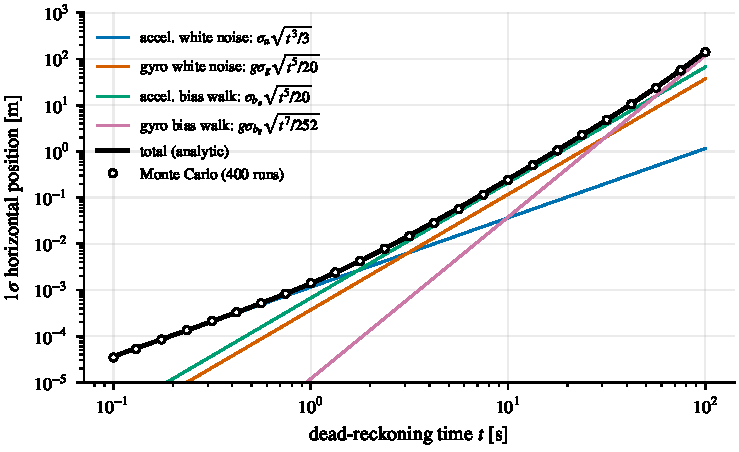
\includegraphics[width=0.88\textwidth]{fig_cov_growth.pdf}
  \caption{Horizontal position standard deviation of a dead-reckoning IMU with EuRoC noise parameters,
  from \eqref{eq:growth-laws}, with a Monte Carlo check (400 runs of the discretized error equations at
  200~Hz). Accelerometer white noise dominates for the first two seconds, the accelerometer bias walk from
  there to about a minute, and then the gyro bias walk takes over with its $t^{7/2}$ growth.}
  \label{fig:cov-growth}
\end{figure}

\begin{proposition}[Dead-reckoning growth laws]
\label{prop:growth-laws}
For a level, stationary IMU with zero initial uncertainty, the horizontal position variance grows as
\begin{equation}
  \sigma_p^2(t) = \underbrace{\frac{\sigma_a^2 t^3}{3}}_{\text{accel.\ white}}
  + \underbrace{\frac{g^2\sigma_g^2 t^5}{20}}_{\text{gyro white}}
  + \underbrace{\frac{\sigma_{b_a}^2 t^5}{20}}_{\text{accel.\ bias walk}}
  + \underbrace{\frac{g^2\sigma_{b_g}^2 t^7}{252}}_{\text{gyro bias walk}} .
  \label{eq:growth-laws}
\end{equation}
\end{proposition}
\begin{proof}
Accelerometer white noise is integrated twice ($m = 2$ in \cref{prop:integrated-noise}). Gyro white noise is integrated
once into tilt, scaled by $g$, and integrated twice more ($m = 3$). The accelerometer bias random walk is
itself integrated white noise, then integrated twice ($m = 3$). The gyro bias random walk adds one more
integration ($m = 4$). The sources are independent, so their variances add.
\end{proof}



\Cref{fig:cov-growth} evaluates \eqref{eq:growth-laws} with EuRoC's parameters. After one second of blind flight the
position uncertainty is about 1~mm, after ten seconds about 25~cm, and after a minute more than 10~m. The
camera's job is to keep the filter permanently in the left part of this plot.

\begin{projectlink}[Milestone 5]
The analytic check of M5 isolates the first term of \eqref{eq:growth-laws}: with $P_0 = 0$, only accelerometer noise and a
fixed orientation, the horizontal position variance must equal $\sigma_a^2t^3/3$. Because $\Phi$ and $Q_d$ are first-order
approximations, the agreement improves as $\Dt\to0$ (\cref{ex:double-integrator-qd}), and the test tolerance should reflect
that.
\end{projectlink}

\paragraph{Why diagonal entries need not grow monotonically.} The attitude covariance is expressed in body axes
(\cref{rem:cov-rotates}). When the vehicle rotates, the attitude block of $\Phi$ rotates the covariance between axes, so an
individual diagonal entry can shrink during pure propagation even though no information is gained. Monotonicity
holds for invariant quantities, such as the eigenvalues of $P_{\theta\theta}$ when the vehicle is not rotating, but not for
individual entries.

% ------------------------------------------------------------------------------
\section{Validating covariance propagation}

Two independent tests catch nearly all propagation bugs.

\paragraph{Finite differences on the discrete propagation.} The Jacobian of one step of the nominal integrator,
computed numerically with $\bplus/\bminus$, must match $\Phi$ column by column (the derivation exercise above). This
catches sign errors, transposes, and blocks placed at wrong indices. The test must use a non-trivial state.

\paragraph{Monte Carlo.} Simulate $M$ noisy IMU sequences from a known trajectory, integrate each with the nominal
equations from a perturbed initial state drawn from $P_0$, and compute the errors
$e^{(j)} = x_{\text{true}}\bminus\hat x^{(j)}$. Their sample covariance must agree with the propagated $P$. If the filter is
correct, the ratio of a sample variance to the predicted variance is distributed as $\chi^2_{M-1}/(M-1)$, so for
$M = 500$ it should lie in $[0.88, 1.13]$ with 95\% probability for each diagonal entry. Larger deviations, or many
entries near the bounds in the same direction, indicate an error in $G_c$, $Q_c$ or the units. This catches errors
that finite differences cannot, such as a wrong noise density or a missing $\Dt$.

\begin{takeaways}
\begin{itemize}
  \item The error state is 15-dimensional with the frozen layout $[\delta p, \delta v, \delta\theta, \delta b_a, \delta b_g]$.
  \item Error dynamics follow from substituting $x = \hat x\bplus\delta x$, subtracting the nominal dynamics, and keeping
        first-order terms. The perturbation convention changes the result.
  \item $\Phi \approx I + F_c\Dt$, $Q_d \approx G_cQ_cG_c\T\Dt$ with continuous densities; clones have identity dynamics.
  \item Position variance grows like $t^3$ (accel.\ noise), $t^5$ (gyro noise, accel.\ bias walk) and $t^7$ (gyro bias walk).
  \item Validate $\Phi$ by finite differences and $P$ by Monte Carlo with statistically justified bounds.
\end{itemize}
\end{takeaways}

\begin{exercises}
  \item Derive the velocity error dynamics for the global perturbation, and compare its structure with your local
        result. Which one depends on the vehicle's heading?
  \item Using your $F_c$, show that $\delta\theta$ is decoupled from $\delta p$ and $\delta v$, and explain this from the cascade structure.
  \item Starting from \eqref{eq:imu-discretization}, write $Q_d$ block by block and check its units.
  \item Implement covariance propagation for the 15-state system in Python and reproduce \cref{fig:cov-growth}, including
        the Monte Carlo points.
  \item For a vehicle rotating about its $z$-axis at 1~rad/s with $P_{\theta\theta} = \diag(10^{-4}, 10^{-6}, 10^{-6})$, propagate
        $P_{\theta\theta}$ for a quarter turn with no noise and observe the diagonal entries.
  \item How large must $M$ be for a Monte Carlo variance check to detect a 10\% error in $\sigma_a$ with high probability?
\end{exercises}


\part{The Error-State Filter in Practice}
\chapter{Measurement Updates, Gating and the Pose Sensor}
\label{ch:updates}
\chaptermark{Measurement Updates} % short running header

\begin{objectives}
\begin{itemize}
  \item Apply the generic manifold update to concrete sensors, deriving $H$ by the elementary Jacobians.
  \item Understand which state directions a measurement observes, from the nullspace of $H$.
  \item Implement the mock pose sensor of Milestone 6 and derive its Jacobian.
  \item Gate measurements with the $\chi^2$ test, and understand how gating fails in an overconfident filter.
  \item Understand how a pose sensor makes velocity and biases observable.
\end{itemize}
\end{objectives}

% ------------------------------------------------------------------------------
\section{The generic update}

\begin{convention}[measurement update, AGENTS.md F3]
\begin{enumerate}
  \item Residual $r = z\bminus h(\hat x)$: plain subtraction for vector measurements; for the pose measurement
        $r = [\,p_{meas} - \hat p;\ \Log_q(\hat q\inv\qprod q_{meas})\,]$.
  \item $H = \partial r/\partial\delta x$ at $\delta x = 0$ using C4 (\cref{sec:manifold-update}), derived by hand and verified by
        finite differences.
  \item $S = HPH\T + R_z$; $K = PH\T S\inv$ by a Cholesky/LDL$^\mathsf{T}$ solve, never an explicit inverse.
  \item Mahalanobis gate $r\T S\inv r < \chi^2_{0.95}(\dim r)$ from a \code{constexpr} table. Rejections are counted and
        logged, never silently dropped.
  \item Joseph form $P \gets (I - KH)P(I - KH)\T + KR_zK\T$, then injection and reset (\cref{sec:reset}).
\end{enumerate}
\end{convention}

Everything specific to a sensor is in $h$ and $H$. The rest of this section derives them for two sensors that the
project does not use, to demonstrate the technique, before turning to the pose sensor it does use.

% ------------------------------------------------------------------------------
\section{Worked example: position with a lever arm}

A GNSS antenna mounted at a known offset $\ell_b$ from the IMU, expressed in the body frame, measures the
antenna position:
\begin{equation}
  z = h(x) + n = p_{wb} + R_{wb}\,\ell_b + n, \qquad n \sim \N(0, \sigma^2I_3).
\end{equation}
The residual is a plain difference, $r = z - (\hat p + \hat R\ell_b)$. To find $H$, perturb the nominal state with
$\bplus$ and expand:
\begin{equation*}
  h(\hat x\bplus\delta x) = \hat p + \delta p + \hat R\Exp(\delta\theta)\ell_b
  \approx \hat p + \delta p + \hat R\ell_b + \hat R\sx{\delta\theta}\ell_b
  = h(\hat x) + \delta p - \hat R\sx{\ell_b}\delta\theta .
\end{equation*}
Reading off the coefficients (the rotation-action row of \cref{tab:jacobians}),
\begin{equation}
  H = \begin{bmatrix} I_3 & 0_3 & -\hat R\sx{\ell_b} & 0_3 & 0_3 \end{bmatrix}.
\end{equation}
The attitude column is non-zero because the antenna swings around the IMU when the body rotates. A
lever-arm position measurement therefore carries attitude information, but only about rotations that move
the antenna: the nullspace of $-\hat R\sx{\ell_b}$ is the direction $\ell_b$, since rotating about the lever arm itself
does not move the antenna.

% ------------------------------------------------------------------------------
\section{Worked example: a direction sensor}

A magnetometer, or an accelerometer used as an inclinometer at rest, measures a known world vector $m_w$ in
body coordinates:
\begin{equation}
  z = R_{wb}\T m_w + n .
\end{equation}
With the inverse-action row of \cref{tab:jacobians}, $h(\hat x\bplus\delta x) = \Exp(-\delta\theta)\hat R\T m_w \approx \hat R\T m_w +
\sx{\hat R\T m_w}\delta\theta$, so
\begin{equation}
  H = \begin{bmatrix} 0_3 & 0_3 & \sx{\hat R\T m_w} & 0_3 & 0_3 \end{bmatrix}.
\end{equation}
$\sx{v}$ has rank two and nullspace $\mathrm{span}(v)$, so a direction measurement observes two of the three attitude
degrees of freedom. The rotation about the measured direction is unobservable. For gravity this is the
familiar statement that an accelerometer at rest gives roll and pitch but not yaw.

\begin{keyidea}[the nullspace of $H$ tells you what a sensor cannot see]
Any error direction $\delta x \in \nullsp(H)$ produces no change in the predicted measurement, so the update cannot
correct it. Reading the nullspace of each new $H$ is a quick sanity check of both the derivation and your
intuition about the sensor.
\end{keyidea}

% ------------------------------------------------------------------------------
\section{The pose sensor of Milestone 6}

Before introducing a camera, the project tests the whole ESKF with a ``mock sensor'' that measures the pose
directly. Ground-truth poses, decimated to about 10~Hz, are corrupted with synthetic noise of known statistics.

\begin{convention}[pose measurement, AGENTS.md C6]
\begin{equation}
  p_{meas} = p_{wb} + n_p, \qquad q_{meas} = q_{wb}\qprod\Exp_q(n_\theta), \qquad
  R_z = \diag(\sigma_p^2 I_3,\ \sigma_\theta^2 I_3).
\end{equation}
\end{convention}

The attitude noise is applied on the right, in the body frame, which is exactly the local perturbation. That
choice makes the residual \eqref{eq:manifold-residual} statistically clean: if the nominal state were exact, the
attitude residual would be exactly $n_\theta$. To generate the noise, draw $n_p$ and $n_\theta$ from seeded
\code{std::mt19937\_64} generators (AGENTS.md E5) with the same $\sigma_p$, $\sigma_\theta$ that appear in $R_z$.

\begin{derivex}{the pose measurement Jacobian $H \in \R^{6\times15}$}{sol:Hpose}
Using \eqref{eq:manifold-H}, derive $H$ for $h(x) = (p_{wb}, q_{wb})$ with the residual of AGENTS.md F3.
\begin{enumerate}
  \item The position rows are a plain difference. Which state blocks does $\hat p + \delta p$ depend on?
  \item For the attitude rows, evaluate $\Log_q\big(\hat q\inv\qprod(\hat q\qprod\Exp_q(\delta\theta))\big)$ and simplify.
        Which elementary Jacobian applies if you instead linearize around a non-zero residual?
  \item Write $H$ in the frozen column order and state its nullspace. Which states are \emph{not} directly measured,
        and how can they still be corrected?
\end{enumerate}
\textbf{Check:} the finite-difference test of $r(\delta x) = h(\hat x\bplus\delta x)\bminus h(\hat x)$ at a non-trivial state, as
required by Milestone 6.
\end{derivex}

\paragraph{How unmeasured states get corrected.} The pose sensor measures neither velocity nor biases, yet the
update corrects both. The mechanism is the cross-covariance built up by propagation. Between updates, a velocity
error produces a growing position error, so $P_{pv}$ becomes large; an accelerometer bias produces a velocity error
and then a position error, so $P_{p b_a}$ grows; a gyro bias produces an attitude error, so $P_{\theta b_g}$ grows. The gain
$K = PH\T S\inv$ has non-zero rows for every state correlated with the measured ones, so each pose update corrects
them in proportion to those correlations.

\paragraph{Why the biases converge.} Observability here has an intuitive reading. The gyro bias is the slope of the
difference between the integrated gyro and the measured attitude, which a sequence of attitude measurements reveals.
The velocity is the slope of the measured position. The accelerometer bias is the difference between the
acceleration implied by successive velocities and the specific force rotated with the (measured) attitude, so it
too becomes observable. Even at rest it is separable from tilt, because the attitude is measured directly. With
pose measurements every state of the IMU error state is observable, and their covariances converge.

% ------------------------------------------------------------------------------
\section{Gating}
\label{sec:gating}

Real measurements include outliers: a misassociated feature, a reflection, a moving object. A single outlier with a
large residual can drag the estimate far away and corrupt the covariance. The $\chi^2$ test of \cref{prop:innovation}
rejects measurements that are statistically implausible given the filter's own uncertainty:
\begin{equation}
  \gamma = r\T S\inv r \ \stackrel{?}{<}\ \chi^2_{1-\alpha}(\dim r).
\end{equation}

\begin{table}[h]
\centering\small
\begin{tabular}{@{}c c c c c c c@{}}
\toprule
$\dim r$ & 1 & 2 & 3 & 4 & 5 & 6 \\
\midrule
$\chi^2_{0.95}$ & 3.841 & 5.991 & 7.815 & 9.488 & 11.070 & 12.592 \\
$\chi^2_{0.99}$ & 6.635 & 9.210 & 11.345 & 13.277 & 15.086 & 16.812 \\
\bottomrule
\end{tabular}
\caption{Gate thresholds. A longer table, up to 600 degrees of freedom, is in \cref{app:tables}.}
\label{tab:chi2-short}
\end{table}

With a 95\% gate, a consistent filter rejects 5\% of perfectly good measurements. That is the price of rejecting
most outliers, and it is why rejections are counted and logged: a rejection rate close to 5\% is a sign of
health, a rate near zero suggests an underconfident filter (or a gate that is too loose to be useful), and a
rate far above 5\% indicates overconfidence or a model error.

\begin{pitfall}[the death spiral]
Gating assumes the filter is consistent. If $P$ is too small, good measurements produce large $\gamma$ and are
rejected; with no corrections $P$ should grow, but if the model's process noise is also too small it grows slowly
while the true error grows quickly, and more measurements are rejected. The filter then dead-reckons with false
confidence until it diverges. When the rejection rate jumps, suspect overconfidence before suspecting outliers.
\end{pitfall}

The threshold depends on the dimension of $r$. A pose measurement uses $\chi^2_{0.95}(6)$, a single image
observation $\chi^2_{0.95}(2)$, and a projected MSCKF feature residual $\chi^2_{0.95}(2M-3)$, where $M$ is the number of
observations (\cref{ch:msckfupdate}). Because the quantiles grow with the dimension, the table is generated offline
and stored as a \code{constexpr} array, which avoids depending on a statistics library in the core.

% ------------------------------------------------------------------------------
\section{Pseudo-measurements and timing}

\paragraph{Pseudo-measurements.} Knowledge that is not a sensor reading can be fed to the filter as if it were one. The most useful is the \term{zero-velocity
update} (ZUPT): when the vehicle is known to be at rest (detected, for example, from a very small variance of the accelerometer and gyroscope readings over
a window), apply the measurement $z = 0 = v_{wb} + n$ with $H = [0\ \ I_3\ \ 0\ \ 0\ \ 0]$ and a small noise covariance. It stops velocity drift, and through the
correlations it also refines tilt and biases. A ZUPT applied when the vehicle is in fact moving is a large, confident, wrong measurement; the detection must
be conservative. Similar pseudo-measurements express a known constant altitude, a non-holonomic constraint (a car does not slide sideways), or a
known landmark.

\paragraph{Measurement timing.} A measurement taken at time $t_z$ must be applied to the state at $t_z$, after propagating exactly to that time
(\cref{ch:strapdown}). Measurements that arrive \emph{late}, after the filter has already propagated past their timestamp, are a problem for every filter:
either the filter buffers the IMU data and re-propagates from $t_z$, or it uses a stochastic clone of the state at $t_z$ (\cref{ch:cloning}), which is exactly the
MSCKF's approach for camera measurements. On EuRoC, data are processed offline in timestamp order, so late measurements do not occur.

% ------------------------------------------------------------------------------
\section{Testing the update}

\begin{projectlink}[Milestone 6]
The exit criteria test properties that hold for any correct implementation:
\begin{itemize}
  \item $H$ passes the finite-difference test at a non-trivial state;
  \item $P_{prior} - P_{post}$ is positive semi-definite (an update never adds uncertainty);
  \item after injection and reset all quaternions are unit, and a second update with the same $z$ produces a residual
        consistent with the first correction;
  \item as $R_z \to 0$ the posterior pose converges to $z$;
  \item with constant synthetic biases, the bias estimates converge to within their own $3\sigma$;
  \item update, injection and reset do not allocate;
  \item a full MH\_01 run with noisy ground-truth updates neither diverges nor produces NaN, and the $\chi^2$ rejection
        count is logged.
\end{itemize}
\end{projectlink}

The ``second update'' test is subtle and worth understanding. After the first update, the nominal pose has moved
toward $z$ by $K r$, so the second residual should be approximately $(I - HK)r$, which is smaller. If it is instead
larger, or has the opposite sign, the injection used the wrong side of the quaternion product or the wrong sign of
$H$.

\begin{takeaways}
\begin{itemize}
  \item Derive $H$ by perturbing $h(\hat x\bplus\delta x)$, expanding to first order and reading off coefficients.
  \item The nullspace of $H$ lists the error directions a sensor cannot see.
  \item The pose sensor's attitude noise is a local perturbation, matching the residual $\Log_q(\hat q\inv\qprod q_{meas})$.
  \item Unmeasured states are corrected through cross-covariances built up by propagation.
  \item Gate with $\chi^2_{0.95}(\dim r)$, log the rejections, and treat a high rejection rate as a symptom of overconfidence.
\end{itemize}
\end{takeaways}

\begin{exercises}
  \item For the lever-arm example, compute $S$ and $K$ for a state with
        \[ P = \diag(\sigma_p^2I,\ \sigma_v^2I,\ \sigma_\theta^2I,\ \sigma_{b_a}^2I,\ \sigma_{b_g}^2I). \]
        Which components of $\delta\theta$ does the update correct?
  \item Derive $H$ for a range measurement to a known beacon $b_w$: $z = \|p_{wb} - b_w\| + n$. What is its nullspace?
  \item Simulate the death spiral: run a 1D constant-velocity filter with $Q$ underestimated by a factor of 100 and a
        95\% gate. Plot the rejection rate and the error over time.
  \item Show that with a pose measurement of a static vehicle, the horizontal accelerometer bias is observable.
        (Hint: what does the attitude measurement remove from the tilt/bias ambiguity of \cref{ch:strapdown}?)
  \item Prove that $P_{prior} - P_{post} = KSK\T \succeq 0$ for the optimal gain, and explain why this test can fail in floating
        point if the simple covariance update is used.
\end{exercises}
\input{chapters/solutions/18_updates}

\chapter{Consistency and Evaluation}
\label{ch:consistency}

\begin{objectives}
\begin{itemize}
  \item Test whether a filter's covariance tells the truth, with NEES, NIS and $3\sigma$ coverage.
  \item Compute exact statistical bounds for single-run and Monte Carlo tests.
  \item Diagnose over- and under-confidence and tune noise parameters without cheating.
  \item Measure trajectory accuracy with ATE and RPE, using the alignment appropriate for VIO.
\end{itemize}
\end{objectives}

A filter produces two things: an estimate and a covariance. Most evaluations look only at the first. But a
filter with good average accuracy and a covariance that is too small is dangerous: it rejects valid measurements,
it reports false confidence to whatever consumes its output, and it eventually diverges. This chapter is about
checking the second output.

% ------------------------------------------------------------------------------
\section{What consistency means}

Recall from \cref{ch:prob} that a filter reporting $(\hat x_k, P_k)$ is consistent if its error $e_k = x_k\bminus\hat x_k$ has
zero mean and covariance $P_k$. Together with \cref{prop:innovation}, a consistent, correctly modeled filter
satisfies three testable properties:
\begin{enumerate}
  \item estimation errors are compatible with $P_k$ (tested with NEES, needs ground truth);
  \item innovations are compatible with $S_k$ (tested with NIS, needs no ground truth);
  \item innovations are white (tested with autocorrelation, needs no ground truth).
\end{enumerate}
The error must be computed with the manifold difference $\bminus$, using exactly the same convention as the
filter's covariance. Comparing a local-perturbation covariance with a global attitude error, or with an Euler
angle difference, produces meaningless statistics.

% ------------------------------------------------------------------------------
\section{Normalized estimation error squared}

\begin{definition}[NEES]
The normalized estimation error squared at time $k$ is
\begin{equation}
  \epsilon_k = e_k\T P_k\inv e_k, \qquad e_k = x_k\bminus\hat x_k .
\end{equation}
\end{definition}

If the filter is consistent and its errors are Gaussian, $\epsilon_k \sim \chi^2_n$ with $n = \dim e$ by
\cref{thm:mahalanobis-chi2}: its expected value is $n$. A single run gives one sample per time step, which is noisy.
Monte Carlo runs average it out. With $N$ independent runs, the average NEES
$\bar\epsilon_k = \frac1N\sum_{j=1}^N\epsilon_k^{(j)}$ satisfies $N\bar\epsilon_k \sim \chi^2_{Nn}$, so the two-sided 95\% interval is
\begin{equation}
  \left[\ \frac{\chi^2_{0.025}(Nn)}{N},\ \frac{\chi^2_{0.975}(Nn)}{N}\ \right].
  \label{eq:anees-bounds}
\end{equation}
For the 15-state IMU filter with $N = 50$ runs this is $[13.52, 16.56]$; for $N = 100$, $[13.95, 16.09]$.
\Cref{app:tables} lists more. Average NEES above the interval means overconfidence (errors larger than claimed);
below means underconfidence.

\begin{figure}[t]
  \centering
  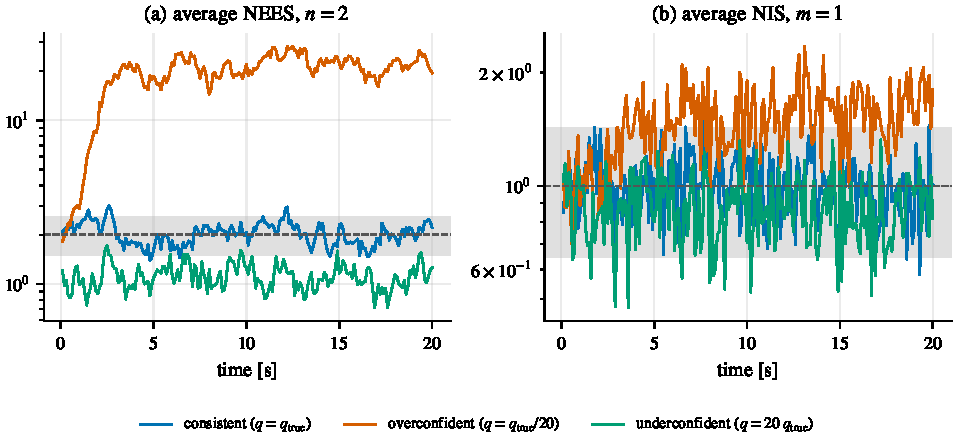
\includegraphics[width=\textwidth]{fig_nees.pdf}
  \caption{Consistency statistics of a constant-velocity filter over 50 Monte Carlo runs, with the 95\%
  acceptance region (gray) of \eqref{eq:anees-bounds}. Underestimating the process noise by a factor of 20 makes the
  filter overconfident: the NEES leaves the region by an order of magnitude, and the NIS rises above it. Overestimating
  it makes the filter underconfident: the NEES falls below the region. Note that the NIS of the underconfident filter
  is less clearly abnormal: NIS alone is a weak detector of underconfidence.}
  \label{fig:nees}
\end{figure}

\paragraph{Block NEES.} The NEES of the full state mixes well-estimated and poorly estimated blocks. Computing it
separately for position, velocity, attitude and biases, each with its own $3\times3$ block of $P$ and $\chi^2_3$ bounds, points
directly at the misbehaving part.

% ------------------------------------------------------------------------------
\section{Normalized innovation squared}

\begin{definition}[NIS]
$\nu_k = r_k\T S_k\inv r_k$, the same quantity the gate computes.
\end{definition}

Under consistency $\nu_k \sim \chi^2_m$ with $m = \dim r_k$. NIS needs no ground truth, so it is the main consistency
monitor on real data. Two summaries are useful: the fraction of updates with $\nu_k$ below its 95\% quantile, which
should be close to 95\% (Milestone 7), and the time-average of $\nu_k$, which should be close to $m$. If measurements have
different dimensions, normalize by $m_k$ or compare each against its own quantile.

\paragraph{$3\sigma$ coverage.} For each scalar component $i$, a consistent Gaussian error lies within $\pm3\sqrt{P_{ii}}$
99.7\% of the time. Plotting errors against their $3\sigma$ envelopes is the most readable diagnostic, and the coverage
fraction is a simple scalar summary. On EuRoC, Milestone 7 requires at least 95\% coverage for velocity and biases.
These states are not measured by the pose sensor, so their consistency is not circular.

% ------------------------------------------------------------------------------
\section{Diagnosing inconsistency}

\begin{table}[t]
\centering\small
\begin{tabularx}{\textwidth}{@{}l l X@{}}
\toprule
\textbf{NEES} & \textbf{NIS} & \textbf{Likely causes} \\
\midrule
high & high & process noise too small; wrong noise units (missing $\Dt$ or $\sqrt{\Dt}$); unmodeled IMU errors; integration error \\
high & normal & errors in directions the measurement does not see (unobservable states, e.g.\ yaw in VIO); wrong $\bminus$ convention in the evaluation \\
normal & high & measurement noise too small; outliers passing the gate; wrong $H$ \\
low & low & process or measurement noise too large \\
high, growing & normal & spurious information along unobservable directions (EKF inconsistency, \cref{ch:observability}) \\
spikes & spikes & time-synchronization errors; wrong extrinsics; bad initialization \\
\bottomrule
\end{tabularx}
\caption{Reading consistency statistics. Combinations narrow the search for the bug.}
\label{tab:consistency-diagnosis}
\end{table}

\Cref{tab:consistency-diagnosis} is a starting point for debugging. Two additional checks are valuable. First, plot each
residual component over time: a non-zero mean reveals a bias (wrong extrinsics, a wrong sign in $h$); slow oscillation
reveals correlated errors (a coloured noise the filter assumes white). Second, compare the covariance with Monte
Carlo statistics on synthetic data, where the truth is known exactly and the noise is exactly as modeled. If the filter
is inconsistent on synthetic data, the bug is in the filter. If it is consistent there but not on real data, the problem is
the model.

\subsection{Tuning without cheating}

\begin{enumerate}
  \item \textbf{Synthetic first.} With synthetic data generated with exactly the filter's noise parameters, there is
        nothing to tune: a consistent implementation must pass. Any failure is a bug.
  \item \textbf{Physically meaningful knobs only.} On real data, adjust the IMU noise densities (start from
        \cref{tab:euroc-imu}, inflate modestly for unmodeled effects) and the measurement noise (start from the pixel
        noise of the detector). Do not add arbitrary noise to arbitrary states.
  \item \textbf{Judge on consistency, not accuracy.} Choose parameters that make NIS and coverage statistics correct.
        Lower trajectory error obtained by making the filter inconsistent will not generalize.
  \item \textbf{Separate tuning from evaluation.} Tune on some sequences and report results on others.
  \item \textbf{Ground truth never enters the filter} except where explicitly allowed and logged (initialization).
\end{enumerate}

% ------------------------------------------------------------------------------
\section{Trajectory accuracy}

Consistency says whether the covariance is honest; accuracy says how small the errors are. VIO accuracy is
reported with two metrics~\cite{sturm2012tum, zhang2018tutorial}.

\subsection{Absolute trajectory error}

The estimated trajectory lives in a world frame that is only defined up to the unobservable directions, so it must
be aligned with the ground truth before comparing. Given time-associated positions $p_i$ (ground truth) and
$\hat p_i$ (estimate), find the transformation that best maps the estimate onto the truth, then compute
\begin{equation}
  \mathrm{ATE}_{\mathrm{RMSE}} = \Big(\frac1N\sum_{i=1}^N\big\|p_i - (R^\star\hat p_i + t^\star)\big\|^2\Big)^{1/2}.
\end{equation}
For rigid alignment, the optimal transformation has a closed form (Kabsch/Umeyama~\cite{umeyama1991}).

\begin{proposition}[Optimal rigid alignment]
\label{prop:umeyama}\label{sec:umeyama}
\index{Umeyama alignment}
Let $\mu$ and $\hat\mu$ be the means of the two point sets, $a_i = p_i - \mu$ and $b_i = \hat p_i - \hat\mu$ the centered points, and
$\Sigma_{ab} = \frac1N\sum_ia_ib_i\T = UDV\T$ an SVD. The minimizer of $\sum_i\|p_i - (R\hat p_i + t)\|^2$ over rotations $R$ and translations $t$ is
\begin{equation}
  R^\star = U\diag\big(1, 1, \det(UV\T)\big)V\T, \qquad t^\star = \mu - R^\star\hat\mu .
\end{equation}
\end{proposition}
\begin{proof}
For fixed $R$, the cost is a quadratic in $t$ minimized where its gradient vanishes, $\sum_i(p_i - R\hat p_i - t) = 0$, i.e.\ $t = \mu - R\hat\mu$: the alignment maps
centroid onto centroid. Substituting, the cost becomes $\sum_i\|a_i - Rb_i\|^2 = \sum_i(\|a_i\|^2 + \|b_i\|^2) - 2\sum_ia_i\T Rb_i$, so we must maximize
$\sum_ia_i\T Rb_i = \tr\big(R\sum_ib_ia_i\T\big) = N\tr(R\,VDU\T) = N\tr(D\,Z)$ with $Z = U\T RV$. $Z$ is orthogonal, so its diagonal entries are at most one in
magnitude, and $\tr(DZ) = \sum_id_iZ_{ii} \le \sum_id_i$, with equality for $Z = I$, i.e.\ $R = UV\T$. If $\det(UV\T) = -1$ this is a reflection, not a rotation; the
best rotation then flips the axis with the smallest singular value, $Z = \diag(1, 1, -1)$, which gives the stated formula.
\end{proof}

If the scale is also free (a similarity transform, needed for monocular vision without an IMU), the optimal scale is
$s^\star = \tr(D\,\diag(1, 1, \det(UV\T)))\big/\frac1N\sum_i\|b_i\|^2$, applied as $s^\star R^\star\hat p_i + t^\star$ with $t^\star = \mu - s^\star R^\star\hat\mu$.

\begin{keyidea}[align only what is unobservable]
Which transformation to allow depends on the estimator. Monocular vision alone has a free scale, so it uses a
similarity transform (7 DOF). VIO has metric scale and observable roll and pitch: its unobservable directions are
exactly translation and yaw. The appropriate alignment is therefore 4-DOF (translation plus a rotation about
gravity)~\cite{zhang2018tutorial}. A full 6-DOF alignment would also remove roll and pitch errors that the
estimator was responsible for.
\end{keyidea}

The 4-DOF alignment follows the same proof with $R$ restricted to rotations $R_z(\psi)$ about the vertical. For centered points $a = (x, y, z)$ (truth)
and $b = (\hat x, \hat y, \hat z)$ (estimate), $a\T R_z(\psi)b = (x\hat x + y\hat y)\cos\psi + (y\hat x - x\hat y)\sin\psi + z\hat z$, whose sum over the points is maximized by
\begin{equation}
  \psi^\star = \atantwo\Big(\sum_i(y_i\hat x_i - x_i\hat y_i),\ \sum_i(x_i\hat x_i + y_i\hat y_i)\Big),
  \label{eq:4dof-yaw}
\end{equation}
again with $t^\star = \mu - R_z(\psi^\star)\hat\mu$.

Milestone 10b reports ATE after SE(3) alignment, as in most published benchmarks; reporting the 4-DOF result
alongside it is more faithful to what VIO can know.

\subsection{Relative pose error}

ATE is dominated by the largest drift and depends on trajectory length and shape. The relative pose error (RPE)
compares relative motions over a fixed distance or time $\Delta$:
\begin{equation}
  E_i = \big(T_{i}\inv T_{i+\Delta}\big)\inv\big(\hat T_i\inv\hat T_{i+\Delta}\big),
\end{equation}
and reports statistics of the translation and rotation parts of $E_i$, often as a percentage of distance traveled. It
needs no global alignment and measures local drift, which is what odometry is about. The \code{evo}
package~\cite{grupp2017evo} computes both metrics with all the alignment variants.

\begin{projectlink}[Milestone 7]
M7 logs $\hat x$, $\diag(P)$, ground truth, NIS and NEES to a preallocated buffer, flushes it outside the hot loop, and
plots $3\sigma$ envelopes and NEES/NIS against their $\chi^2$ bounds from a single script. Exit criteria: average NEES inside
the 95\% interval for 15 DOF over most of a $\geq50$-run synthetic Monte Carlo; NIS within its per-update bound for about
95\% of updates; at least 95\% $3\sigma$ coverage of velocity and biases on MH\_01; zero allocations while logging.
\end{projectlink}

\begin{takeaways}
\begin{itemize}
  \item A filter must be judged on the honesty of its covariance as well as its accuracy.
  \item NEES needs ground truth and tests $P$; NIS needs none and tests $S$. Both are $\chi^2$ under consistency.
  \item Monte Carlo averages have exact bounds $[\chi^2_{0.025}(Nn), \chi^2_{0.975}(Nn)]/N$.
  \item Overconfidence (NEES too high) is the dangerous failure; NIS alone detects underconfidence poorly.
  \item Tune physically meaningful parameters for consistency, on synthetic data first.
  \item Report ATE after an alignment matched to the unobservable directions, and RPE for local drift.
\end{itemize}
\end{takeaways}

\begin{exercises}
  \item Show that the single-run NEES of a consistent 15-state filter exceeds its 95\% quantile 5\% of the time. Why
        is the Monte Carlo average a much sharper test?
  \item Reproduce \cref{fig:nees}. Then make only the measurement noise wrong instead of the process noise and compare
        the signatures.
  \item Derive the closed-form 4-DOF alignment above by maximizing $\sum_i p_i\T R_z(\psi)\hat p_i$ over $\psi$.
  \item Explain why the NEES of yaw in a VIO run on real data tends to grow over time even when the NIS looks
        healthy. (Revisit after \cref{ch:observability}.)
  \item Compute the RPE over 10~m segments for a trajectory with a constant yaw drift of $1^\circ$ per minute flying at
        1~m/s. How does it compare with the ATE after a 10-minute flight?
\end{exercises}
\input{chapters/solutions/19_consistency}


\part{Computer Vision}
\chapter{Image Formation and Camera Models}
\label{ch:camera}
\chaptermark{Image Formation} % short running header

\begin{objectives}
\begin{itemize}
  \item Understand how a camera forms an image: pinholes, lenses, focus, sensors, exposure and shutters.
  \item Derive the pinhole projection, the intrinsic matrix and normalized image coordinates.
  \item Use homogeneous coordinates and the basic projective geometry of points, lines and homographies.
  \item Model and invert the radial-tangential lens distortion used by EuRoC, and know the fisheye alternative.
  \item Understand how cameras are calibrated.
  \item State the project's camera measurement model with its noise, derive the projection Jacobian, and understand extrinsics and time offsets.
\end{itemize}
\end{objectives}

% ==============================================================================
\section{How a camera forms an image}

\subsection{From pinhole to lens}

A camera measures the \emph{directions} of light rays. In a \emph{camera obscura}, light from the scene enters a dark box through a tiny hole and
forms an inverted image on the opposite wall: every point of the wall receives light only from the scene point on the straight line through the
hole. This is the \term{pinhole model}, and it is geometrically perfect. It is also impractical: a hole small enough to give a sharp image lets in
very little light.

A lens gathers light through a large aperture and bends it so that all rays from one scene point converge again at one image point. For an ideal
\emph{thin lens} of focal length $f_L$, a point at distance $z_o$ in front of the lens is imaged sharply at distance $z_i$ behind it, where
\begin{equation}
  \frac1{f_L} = \frac1{z_o} + \frac1{z_i} .
\end{equation}
For distant scenes ($z_o \gg f_L$) the image forms at $z_i \approx f_L$, which is where the sensor sits in a camera focused at infinity. Points at other
distances form slightly blurred spots; the range of distances that stays acceptably sharp is the \emph{depth of field}, larger for small apertures and
short focal lengths. The central ray through the lens center is not bent, so the geometry of a focused lens camera is exactly that of a pinhole at
the lens center: the pinhole model describes it, and lens imperfections are added as \emph{distortion} (\cref{sec:distortion}).

\subsection{The image sensor}

The sensor is a grid of light-sensitive \emph{pixels}. Each accumulates charge in proportion to the light it receives during the \emph{exposure time},
and the charge is converted into a number, typically 8 bits per pixel for the monochrome cameras of EuRoC. Several properties of the sensor matter to an
estimator.
\begin{itemize}
  \item \emph{Exposure and motion blur.} A camera rotating at $\omega$ rad/s during an exposure of $T$ seconds smears each point over about $f\omega T$ pixels, with
        $f$ the focal length in pixels. At 1~rad/s, 5~ms and $f = 458$~px this is 2.3~px, enough to degrade feature tracking. EuRoC's difficult
        sequences contain exactly such blur.
  \item \emph{Global versus rolling shutter.} A global shutter exposes all pixels at the same instant, as EuRoC's cameras do. A rolling shutter (common in
        phones) exposes rows one after another, so each row is captured at a different time and, on a moving camera, from a different pose. Rolling-shutter
        images need an extended measurement model.
  \item \emph{Noise and dynamic range.} Pixel values carry photon and electronic noise, and scenes brighter or darker than the sensor's range saturate. Auto
        exposure changes the brightness of the same scene point between frames, which matters for intensity-based tracking (\cref{ch:frontend}).
\end{itemize}

\paragraph{Pixel coordinates.} We write pixel coordinates as $(u, v)$, with $u$ increasing to the right and $v$ increasing downward, and the origin at the
top-left of the image. In OpenCV's convention, integer coordinates are pixel \emph{centers}. The camera frame $C$ is aligned with this: $x_c$ to the right, $y_c$
down, $z_c$ along the optical axis into the scene.

% ==============================================================================
\section{The pinhole projection}

An ideal pinhole camera lets light through a single point, the optical center. A scene point with camera-frame coordinates $p_c = (X, Y, Z)$, with $Z$ along the
optical axis, projects through the center onto an image plane. Placing a virtual image plane at unit distance \emph{in front of} the center (which avoids
the inversion of the physical image) and using similar triangles, the image of the point is
\begin{equation}
  \pi(p_c) = \begin{bmatrix} x \\ y \end{bmatrix} = \begin{bmatrix} X/Z \\ Y/Z \end{bmatrix}.
  \label{eq:pinhole}
\end{equation}
These are the \term{normalized image coordinates}: dimensionless, independent of the lens, and equal to the tangents of the ray's angles from the optical axis.
The vector $\bar x = (x, y, 1)$ is the \term{bearing} of the point, defined up to scale.

\begin{figure}[t]
\centering
\begin{tikzpicture}[scale=1.0]
  \coordinate (O) at (0,0);
  \draw[frameaxis, plotblue] (O) -- (6.2,0) node[right] {$z_c$ (optical axis)};
  \draw[frameaxis, plotorange] (O) -- (0,-1.6) node[below] {$y_c$};
  \fill (O) circle (1.6pt) node[above left] {$C$};
  \draw[thick, primary] (2,1.8) -- (2,-1.4);
  \node[primary, font=\footnotesize, align=center] at (2,2.15) {normalized plane $Z = 1$};
  \coordinate (P) at (5.6,-1.25);
  \fill[plotgreen] (P) circle (2pt) node[right] {$p_c = (X, Y, Z)$};
  \draw[plotgreen, dashed] (O) -- (P);
  \coordinate (I) at (2,{-1.25*2/5.6});
  \fill[conv] (I) circle (1.8pt);
  \node[conv, font=\footnotesize, right] at (2.05,-0.18) {$y = Y/Z$};
  \draw[<->, black!60] (0,0.5) -- (2,0.5) node[midway, above, font=\footnotesize] {$1$};
  \draw[<->, black!60] (0,0.95) -- (5.6,0.95) node[midway, above, font=\footnotesize] {$Z$};
\end{tikzpicture}
\caption{Pinhole projection in the $y$-$z$ plane. The ray from the optical center $C$ to the point intersects the plane $Z = 1$ at height $Y/Z$. All points
along the ray project to the same image point, so depth is lost.}
\label{fig:pinhole}
\end{figure}

\subsection{Intrinsic parameters}

Pixels are obtained by scaling and shifting the normalized coordinates with the \term{intrinsic matrix}:
\begin{equation}
  \begin{bmatrix} u \\ v \\ 1 \end{bmatrix} = K\begin{bmatrix} x \\ y \\ 1 \end{bmatrix}, \qquad
  K = \begin{bmatrix} f_u & s & c_u \\ 0 & f_v & c_v \\ 0 & 0 & 1 \end{bmatrix},
\end{equation}
with focal lengths $f_u, f_v$ in pixels, principal point $(c_u, c_v)$ (where the optical axis pierces the image), and skew $s$ (zero for modern sensors). The
focal length in pixels is the physical focal length divided by the pixel pitch; $f_u \neq f_v$ if pixels are not square. Inverting $K$ turns a pixel into a bearing,
$\bar x = K\inv(u, v, 1)\T$. The horizontal \emph{field of view} of a $W$-pixel-wide image is $2\arctan\big(W/(2f_u)\big)$, ignoring distortion. EuRoC's \code{cam0} has
$f_u = 458.654$, $f_v = 457.296$, $c_u = 367.215$, $c_v = 248.375$ on a $752\times480$ sensor: a horizontal field of view of about $79^\circ$.

% ==============================================================================
\section{Homogeneous coordinates and projective geometry}
\label{sec:homogeneous}

\subsection{Points and lines in the image}

\index{homogeneous coordinates}
The image point $(x, y)$ corresponds to the whole ray of 3D vectors $\lambda(x, y, 1)$, $\lambda \ne 0$. \term{Homogeneous coordinates} make this explicit: a point of the
plane is represented by any non-zero 3-vector $\tilde x = (x_1, x_2, x_3)$, with $\tilde x$ and $\lambda\tilde x$ representing the same point, and the ordinary coordinates
are recovered as $(x_1/x_3, x_2/x_3)$. Vectors with $x_3 = 0$ represent \emph{points at infinity}: directions, where parallel lines meet.

A line $ax + by + c = 0$ is represented by the 3-vector $l = (a, b, c)$, also up to scale, and a point lies on it exactly when
\begin{equation}
  l\T\tilde x = 0 .
\end{equation}
This symmetric relation makes two constructions one-liners:
\begin{itemize}
  \item the line through two points is $l = \tilde x_1\times\tilde x_2$ (it is orthogonal to both, so both lie on it);
  \item the intersection of two lines is $\tilde x = l_1\times l_2$ (by the same argument).
\end{itemize}
Two parallel lines $(a, b, c_1)$ and $(a, b, c_2)$ intersect at $(b, -a, 0)$ times a constant: a point at infinity in their common direction. In an image of a
3D scene, parallel 3D lines are generally not parallel in the image and meet at a finite \emph{vanishing point}, the image of their common direction.

\subsection{Homographies}

\begin{definition}[Homography]
\index{homography}
A \term{homography} (projective transformation) of the plane is a map $\tilde x \mapsto H\tilde x$ for an invertible $3\times3$ matrix $H$, defined up to scale (eight
degrees of freedom).
\end{definition}

Homographies map lines to lines (if $l\T\tilde x = 0$ then $(H\mT l)\T(H\tilde x) = 0$) but do not preserve parallelism, lengths or angles. Two situations in
which they arise are central to vision:
\begin{itemize}
  \item the images of a \emph{plane} in two views are related by a homography (\cref{ch:multiview}), which is the basis of camera calibration below;
  \item two images taken by a camera that only \emph{rotates} are related by the homography $KRK\inv$, independently of the scene (\cref{ch:multiview,ch:frontend}).
\end{itemize}

\subsection{The projection matrix}

In homogeneous coordinates the complete projection of a world point $p_w$ (with homogeneous coordinates $\tilde p_w = (p_w, 1)$) into pixels is a single linear map,
\begin{equation}
  \lambda\begin{bmatrix} u \\ v \\ 1\end{bmatrix} = K\begin{bmatrix} R_{cw} & p_{cw}\end{bmatrix}\tilde p_w = P\,\tilde p_w,
  \qquad P = K\,[R_{cw}\ \ p_{cw}] \in \R^{3\times4},
\end{equation}
where $(R_{cw}, p_{cw})$ maps world coordinates into the camera frame and $\lambda = Z$ is the depth. The \emph{camera matrix} $P$ has eleven degrees of freedom (twelve
entries up to scale): five intrinsic and six extrinsic. Linear methods that estimate $P$, $H$ or the essential matrix from correspondences
(\cref{ch:multiview}) all exploit the fact that projection is linear in homogeneous coordinates.

% ==============================================================================
\section{Lens distortion}
\label{sec:distortion}

Real lenses bend rays, most strongly near the image edges, so the image of a straight line is curved. The \term{radial-tangential} (Brown--Conrady) model
used by EuRoC maps ideal normalized coordinates $(x, y)$ to distorted ones $(x_d, y_d)$:
\begin{align}
  x_d &= x\,(1 + k_1r^2 + k_2r^4) + 2p_1xy + p_2(r^2 + 2x^2), \\
  y_d &= y\,(1 + k_1r^2 + k_2r^4) + p_1(r^2 + 2y^2) + 2p_2xy, \qquad r^2 = x^2 + y^2,
\end{align}
after which $K$ is applied to $(x_d, y_d)$. The \emph{radial} terms ($k_1, k_2$) model the dominant symmetric distortion of a lens; the \emph{tangential} terms ($p_1, p_2$)
model a lens slightly tilted or decentered relative to the sensor. For \code{cam0}, $(k_1, k_2, p_1, p_2) = (-0.2834, 0.07396, 1.94\times10^{-4}, 1.76\times10^{-5})$. The negative
$k_1$ produces \emph{barrel} distortion (\cref{fig:distortion}). At the middle of the left and right image edges the radial factor $1 + k_1r^2 + k_2r^4$ is about $0.79$,
which moves points by about 100 pixels; at the corners it is about $0.73$, a shift of about 160 pixels. Ignoring distortion is therefore not an option.

\begin{figure}[t]
  \centering
  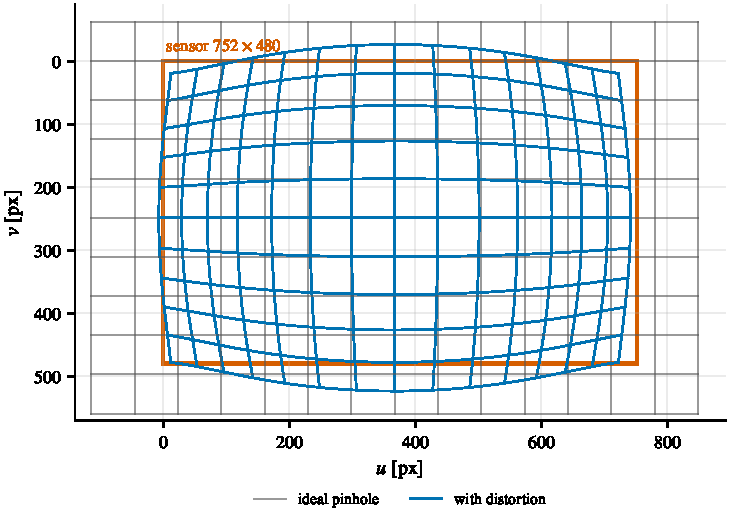
\includegraphics[width=0.84\textwidth]{fig_distortion.pdf}
  \caption{EuRoC \code{cam0} lens distortion. A regular grid in normalized coordinates (gray) is imaged by the real lens as the curved blue grid. Distortion pulls
  points toward the center, increasingly toward the edges, so the sensor (orange) sees a wider field than an ideal pinhole with the same focal length would.}
  \label{fig:distortion}
\end{figure}

\paragraph{Undistortion.} The front end measures distorted pixels and needs ideal normalized coordinates. The model has no closed-form inverse, but a fixed-point
iteration converges quickly for moderate distortion: starting from $x^{(0)} = x_d$,
\begin{equation}
  x^{(j+1)} = \frac{x_d - \Delta_x(x^{(j)}, y^{(j)})}{1 + k_1r_j^2 + k_2r_j^4},\qquad
  y^{(j+1)} = \frac{y_d - \Delta_y(x^{(j)}, y^{(j)})}{1 + k_1r_j^2 + k_2r_j^4},
\end{equation}
where $\Delta$ denotes the tangential terms. A Gauss--Newton iteration (\cref{ch:nlls}) with the $2\times2$ Jacobian of the distortion converges faster and more
reliably near the edges. OpenCV's \code{cv::undistortPoints} implements the iterative scheme. Milestone 8 checks undistortion by distorting and undistorting a
grid of points.

\begin{keyidea}[undistort points, not images]
The estimator needs a few hundred feature locations, not a rectified image. Undistorting only the tracked points costs microseconds; remapping a full image
costs milliseconds, resamples the pixels (blurring them), and changes the noise of the feature detector in a position-dependent way. Track in the raw image and
undistort the tracks.
\end{keyidea}

\paragraph{Wide-angle lenses.} Beyond about $120^\circ$ of field of view, the pinhole model itself breaks down (a ray at $90^\circ$ from the axis would have infinite
normalized coordinates). \emph{Fisheye} models parameterize the image radius as a function of the angle $\vartheta$ of the incoming ray, for example the
equidistant (Kannala--Brandt) model $r_d = \vartheta(1 + k_1\vartheta^2 + k_2\vartheta^4 + \cdots)$. The rest of the pipeline is unchanged: everything downstream of
undistortion works with bearings, which can be represented as unit vectors when they are far from the optical axis.

% ==============================================================================
\section{Camera calibration}

How were EuRoC's intrinsics and distortion coefficients obtained? By observing a known calibration target (a checkerboard or grid of markers) in many
images and fitting the camera model to the observed corner positions.

\paragraph{Zhang's method.} Place the target in the plane $Z = 0$ of its own frame. A target point $(X, Y, 0)$ then projects as
$\lambda\tilde u = K[r_1\ r_2\ r_3\ t](X, Y, 0, 1)\T = K[r_1\ r_2\ t](X, Y, 1)\T$: each image of the target is a homography $H = [h_1\ h_2\ h_3] \propto K[r_1\ r_2\ t]$, estimable from
four or more corner correspondences (\cref{ch:multiview}). Because $r_1$ and $r_2$ are orthonormal, $r_1 = \lambda K\inv h_1$ and $r_2 = \lambda K\inv h_2$ give two
constraints on the matrix $\omega = K\mT K\inv$:
\begin{equation}
  h_1\T\omega h_2 = 0, \qquad h_1\T\omega h_1 = h_2\T\omega h_2 .
\end{equation}
These are linear in the entries of the symmetric $\omega$, so three or more images determine it; $K$ follows from a Cholesky factorization of $\omega$. The linear
estimate is then refined, together with the distortion coefficients and each image's pose, by Levenberg--Marquardt (\cref{ch:nlls}) minimizing the
\emph{reprojection error}, the distance between observed and predicted corners. The residual reprojection error after calibration, typically a few tenths of a
pixel, is the standard measure of calibration quality.

\paragraph{Camera--IMU calibration.} The extrinsics $T_{bc}$ and the time offset are calibrated jointly with the IMU, by moving the rig in front of the target
(\cref{ch:imu}).

% ==============================================================================
\section{The measurement model}

\begin{convention}[camera model, AGENTS.md C6]
In normalized, undistorted image coordinates,
\begin{equation}
  p_c = R_{bc}\T\big(R_{wb}\T(p_f - p_{wb}) - p_{bc}\big), \qquad
  z = \begin{bmatrix} p_{c,x}/p_{c,z} \\ p_{c,y}/p_{c,z} \end{bmatrix} + n_{uv},
  \qquad \sigma_{uv} \approx \sigma_{px}/f .
\end{equation}
\end{convention}

The first equation chains the world-to-body and body-to-camera transformations of \eqref{eq:world-to-camera}. The noise model follows from $u = f_u x + c_u$: a pixel
error $\delta u$ corresponds to a normalized error $\delta u/f_u$. With $\sigma_{px} = 1$~px and $f \approx 458$~px, $\sigma_{uv} \approx 2.2\times10^{-3}$. Strictly, distortion makes the
mapping from pixel noise to normalized noise position-dependent, by the inverse of the distortion Jacobian, and $f_u \neq f_v$. Both effects are small for EuRoC and
conventionally ignored, but they are a legitimate refinement.

% ==============================================================================
\section{The projection Jacobian}

\begin{proposition}[Jacobian of the pinhole projection]
\label{prop:proj-jacobian}
\begin{equation}
  \frac{\partial\pi}{\partial p_c} = \frac{1}{Z}\begin{bmatrix} 1 & 0 & -X/Z \\ 0 & 1 & -Y/Z \end{bmatrix}
  = \frac1Z\begin{bmatrix} I_2 & -\pi(p_c) \end{bmatrix}.
\end{equation}
\end{proposition}
\begin{proof}
Differentiate $X/Z$ and $Y/Z$ with the quotient rule: $\partial(X/Z)/\partial X = 1/Z$, $\partial(X/Z)/\partial Z = -X/Z^2$, and similarly for $Y/Z$.
\end{proof}

The Jacobian has rank two, and its nullspace is spanned by $p_c$ itself: moving the point along its viewing ray does not change its image. This is the single-view
loss of depth in differential form, and it is why a feature must be observed from at least two sufficiently different viewpoints before it constrains anything
(\cref{ch:multiview}). The factor $1/Z$ says that distant points have small image motion for a given change in position. They constrain rotation well and
translation poorly.

The full measurement Jacobian with respect to the filter state is the chain-rule product of this matrix with the Jacobian of $p_c$ with respect to the clone pose
and the feature position. Deriving those is part of \cref{ch:msckfupdate}.

\begin{pitfall}[points behind the camera]
\eqref{eq:pinhole} happily projects points with $Z < 0$, flipping their image through the center. A triangulation or linearization that produces a negative depth must
be rejected (the \emph{cheirality} check), not projected. Points with very small positive $Z$ produce huge Jacobians and should be rejected too.
\end{pitfall}

% ==============================================================================
\section{Extrinsics and time offset}

\paragraph{Extrinsic calibration.} The transformation $T_{bc}$ between the IMU and the camera is estimated offline, for EuRoC with Kalibr~\cite{furgale2013kalibr}, and
stored as \code{T\_BS} in \code{cam0/sensor.yaml}. Its rotation is close to a permutation of axes, and its translation is a few centimeters (\cref{app:euroc}). An error of
$\delta\phi$ in the extrinsic rotation biases every predicted bearing by about $\delta\phi$, which looks to the filter like a systematic residual. A translation error matters
mostly for near points. The project treats $T_{bc}$ as exact (AGENTS.md C3). Estimating it online is a stretch goal.

\paragraph{Time offset.} If the camera timestamp differs from the IMU clock by $t_d$, a feature moving across the image at velocity $\dot z$ is measured with an error of
about $\dot z\,t_d$. A 1~ms offset at an image-plane velocity of 0.5 normalized units per second (fast rotation) is an error of $5\times10^{-4}$, a quarter of a pixel.
EuRoC is hardware synchronized, so $t_d \approx 0$; consumer devices can have offsets of tens of milliseconds and must estimate it online~\cite{li2014timeoffset}.

\begin{takeaways}
\begin{itemize}
  \item A focused lens camera has the geometry of a pinhole at the lens center; lens imperfections are modeled as distortion.
  \item Exposure time causes motion blur of about $f\omega T$ pixels; EuRoC's global shutter exposes all pixels at once.
  \item Normalized coordinates $(X/Z, Y/Z)$ are lens-independent bearings; $K$ maps them to pixels.
  \item Homogeneous coordinates make projection linear; lines through points and intersections of lines are cross products; homographies map planes and pure
        rotations between views.
  \item EuRoC's lens has strong barrel distortion; undistort the tracked points, not the images.
  \item Cameras are calibrated by fitting the model to images of a known target, minimizing reprojection error.
  \item $\partial\pi/\partial p_c = \frac1Z[I_2\ \ {-\pi(p_c)}]$; its nullspace is the viewing ray.
\end{itemize}
\end{takeaways}

\begin{exercises}
  \item A lens with $f_L = 4$~mm is focused at infinity. How far must the sensor move to focus on an object at 0.5~m?
  \item Compute the horizontal and vertical fields of view of \code{cam0} with and without distortion.
  \item Compute the intersection of the lines $x + y = 1$ and $x - y = 0$ with homogeneous coordinates, and the line through $(1, 2)$ and $(3, 1)$.
  \item Show that two parallel lines intersect at a point at infinity, and find the vanishing point of the image of a family of parallel 3D lines with
        direction $d$ under the camera $P = K[I\ \ 0]$.
  \item Implement distortion and fixed-point undistortion for the EuRoC model. How many iterations are needed for $10^{-6}$ accuracy at the image corners? Compare
        with Gauss--Newton.
  \item Derive the two linear constraints of Zhang's method from the orthonormality of $r_1$ and $r_2$.
  \item A point at depth 10~m is observed by a camera translating sideways at 1~m/s and rotating at 1~rad/s. Which motion dominates its image velocity? What does
        this imply for the observability of translation from distant points?
\end{exercises}

\chapter{Digital Image Processing}
\label{ch:imageproc}

\begin{objectives}
\begin{itemize}
  \item Treat an image as a sampled function, and filter it by convolution.
  \item Smooth images with Gaussian kernels, and understand separability and cost.
  \item Compute image gradients robustly with derivative-of-smoothing kernels such as Sobel and Scharr.
  \item Understand why images must be blurred before they are down-sampled, and build Gaussian pyramids.
  \item Interpolate images at sub-pixel positions, find local maxima, and refine them to sub-pixel accuracy.
  \item Know how photometric changes affect intensity-based methods.
\end{itemize}
\end{objectives}

Feature detection and tracking (\cref{ch:frontend}) operate on raw pixel arrays: they smooth them, differentiate them, shrink them and sample them between
pixels. This chapter develops these operations from first principles, as far as the front end needs them.

% ==============================================================================
\section{Images as functions}

A grayscale image is a function $I(u, v)$ giving the brightness at image position $(u, v)$, sampled on the integer grid of pixel centers and quantized,
typically to integers between 0 and 255. In memory it is a 2D array indexed by row and column, $I[\text{row}, \text{col}] = I(u = \text{col}, v = \text{row})$; mixing up the
two orders is a classic bug. Color images have three such channels; a monochrome image can be formed as a weighted sum of them. EuRoC's cameras are
monochrome.

Between pixels, $I$ is undefined until we decide how to interpolate it (\cref{sec:interpolation}). Its derivatives must be approximated by differences of
nearby pixels (\cref{sec:image-derivatives}). Both operations are sensitive to noise and to aliasing, which is what the rest of this chapter is about.

% ==============================================================================
\section{Linear filtering}

\subsection{Correlation and convolution}

\index{convolution}
\termi{Linear filtering}{linear filtering} replaces each pixel by a weighted sum of its neighbors, with the weights given by a small array $h$, the \emph{kernel}. Two closely related
forms exist:
\begin{equation}
\begin{aligned}
  \text{correlation:}&\quad (h\star I)[u, v] = \sum_{i,j}h[i, j]\,I[u + i, v + j], \\
  \text{convolution:}&\quad (h * I)[u, v] = \sum_{i,j}h[i, j]\,I[u - i, v - j] .
\end{aligned}
\end{equation}
Convolution flips the kernel; for symmetric kernels the two coincide. Both are \emph{linear} and \emph{shift-invariant}: filtering a shifted image gives the shifted
filtered image. Convolution is also commutative and associative, so a cascade of filters equals a single filter, $h_2 * (h_1 * I) = (h_2 * h_1) * I$. Near the image
border the kernel extends past the edge, and the missing pixels must be invented: by zeros, by replicating the border, or by reflecting the image. Results
within a kernel radius of the border are always less reliable, which is why detectors ignore a margin there.

A $k\times k$ kernel costs $k^2$ multiplications per pixel. A kernel that factors as an outer product of a column and a row, $h = h_vh_u\T$, is \emph{separable}: filtering
with $h$ equals filtering the rows with $h_u$ and then the columns with $h_v$, at a cost of $2k$ per pixel.

\subsection{Smoothing}

Averaging neighbors reduces noise. The simplest kernel, the \emph{box filter}, averages a $k\times k$ square. The \term{Gaussian filter} weights neighbors by
\begin{equation}
  G_\sigma(u, v) = \frac{1}{2\pi\sigma^2}\exp\!\Big(-\frac{u^2 + v^2}{2\sigma^2}\Big) = g_\sigma(u)\,g_\sigma(v), \qquad g_\sigma(x) = \frac{1}{\sqrt{2\pi}\sigma}e^{-x^2/2\sigma^2},
\end{equation}
sampled at integer offsets, truncated at about $\pm3\sigma$ and renormalized to sum to one. The factorization shows that it is separable. The Gaussian is preferred
over the box because it has no sharp edges: its frequency response is itself a Gaussian, which removes high frequencies smoothly without the ripples of the
box filter. Cascading two Gaussian filters gives a Gaussian whose variances add, $G_{\sigma_1}*G_{\sigma_2} = G_{\sqrt{\sigma_1^2 + \sigma_2^2}}$. Small Gaussians are well
approximated by binomial kernels, $\tfrac14[1, 2, 1]$ and $\tfrac1{16}[1, 4, 6, 4, 1]$ in each direction.

% ==============================================================================
\section{Image derivatives}
\label{sec:image-derivatives}

\index{image gradient}
The \term{image gradient} $\nabla I = (I_u, I_v)$ points in the direction of fastest brightness increase, and its magnitude measures the local contrast. It is
approximated by differences, for example the central difference $I_u[u, v] \approx \tfrac12(I[u + 1, v] - I[u - 1, v])$, a correlation with $\tfrac12[-1, 0, 1]$.

Differentiation amplifies noise: a derivative multiplies each frequency component by its frequency, so pixel-to-pixel noise, the highest frequency present,
is amplified most. The remedy is to smooth before differentiating, and since both are convolutions, to combine them into one kernel. The \emph{Sobel}
operator smooths across the derivative direction with $[1, 2, 1]$ and differentiates along it:
\begin{equation}
  S_u = \begin{bmatrix} 1 \\ 2 \\ 1 \end{bmatrix}\begin{bmatrix} -1 & 0 & 1 \end{bmatrix} = \begin{bmatrix} -1 & 0 & 1 \\ -2 & 0 & 2 \\ -1 & 0 & 1 \end{bmatrix},
  \qquad S_v = S_u\T .
\end{equation}
The \emph{Scharr} operator uses $[3, 10, 3]$ instead of $[1, 2, 1]$, which gives gradient directions that are more accurate for all orientations; OpenCV's
Lucas--Kanade tracker uses it. More generally, the \emph{derivative of a Gaussian}, $\partial G_\sigma/\partial u$, smooths and differentiates at a chosen scale $\sigma$.
Whatever the kernel, it is a weighted difference: its entries sum to zero, so it ignores uniform brightness, and its scale must be divided out when absolute
gradient values matter (Sobel's sum of positive weights is 4 times the step, so $S_u\star I \approx 8I_u$).

\begin{figure}[t]
  \centering
  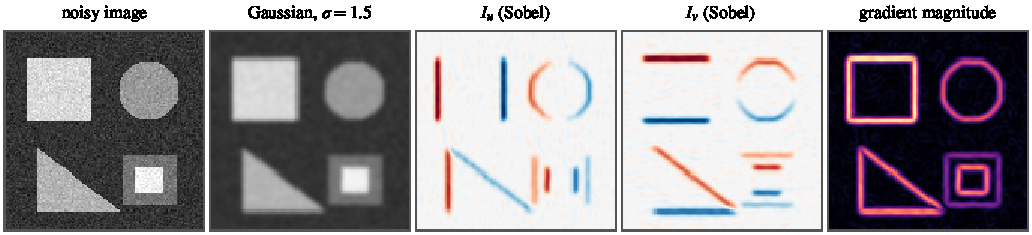
\includegraphics[width=\textwidth]{fig_image_filters.pdf}
  \caption{A synthetic noisy image, its Gaussian smoothing ($\sigma = 1.5$~px), its Sobel derivatives $I_u$ and $I_v$, and the gradient magnitude. Vertical edges respond in
  $I_u$, horizontal edges in $I_v$; corners respond in both, which is what corner detectors look for.}
  \label{fig:image-filters}
\end{figure}

% ==============================================================================
\section{Sampling, aliasing and pyramids}
\label{sec:pyramids}

\subsection{Aliasing in images}

An image is a sampled signal, and the sampling theorem (\cref{ch:processes}) applies in each direction: a pixel grid can represent spatial frequencies up to half a
cycle per pixel. Shrinking an image by keeping every other pixel halves the representable frequency. Any finer detail does not vanish: it \emph{aliases} into false
coarse patterns (moir\'e). The cure is the same as for any sampled signal: low-pass filter, by blurring, before down-sampling.

\begin{figure}[t]
  \centering
  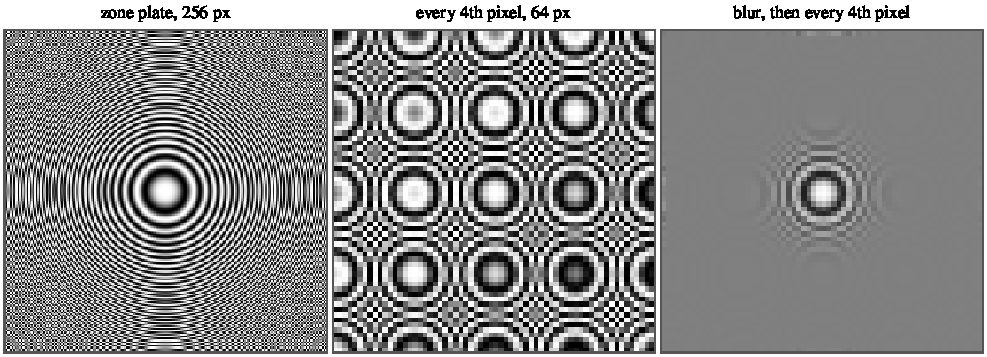
\includegraphics[width=\textwidth]{fig_aliasing_image.pdf}
  \caption{Aliasing in images. A ``zone plate'', whose spatial frequency increases away from the center (left), is shrunk four times by keeping every fourth pixel
  (middle) and by Gaussian blurring first (right). Naive sub-sampling creates false ring patterns; blurring removes the frequencies that cannot be represented.}
  \label{fig:aliasing-image}
\end{figure}

\subsection{Gaussian pyramids}

\index{image pyramid}
A \term{Gaussian pyramid} is a sequence of images, each a blurred and half-resolution copy of the previous one:
\begin{equation}
  I_{\ell+1} = \downarrow_2\big(G * I_\ell\big),
\end{equation}
where $G$ is a small Gaussian (OpenCV's \code{pyrDown} uses the binomial kernel $\tfrac1{16}[1, 4, 6, 4, 1]$ in each direction) and $\downarrow_2$ keeps every second row and
column. Level $\ell$ has $2^{-\ell}$ of the original resolution in each direction, so a pixel position $u_0$ at level 0 corresponds to $u_\ell \approx u_0/2^\ell$ at level $\ell$ (up
to half-pixel conventions). The whole pyramid costs only a third more memory than the original image ($1 + \tfrac14 + \tfrac1{16} + \cdots = \tfrac43$).

\begin{figure}[t]
  \centering
  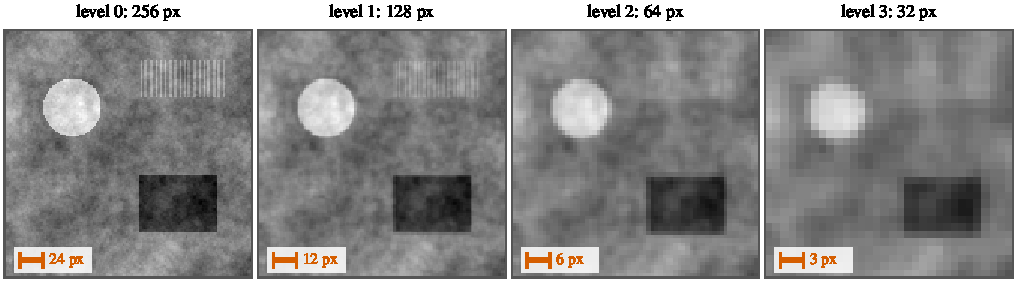
\includegraphics[width=\textwidth]{fig_pyramid.pdf}
  \caption{Four levels of a Gaussian pyramid of a textured synthetic image, displayed at a common size. Fine texture disappears level by level; coarse structure
  survives. A displacement of 24~px at level 0 is a displacement of 3~px at level 3.}
  \label{fig:pyramid-levels}
\end{figure}

Pyramids serve two purposes in the front end. Motion that is large in pixels at full resolution is small at coarse levels, where an iterative tracker can
capture it (\cref{ch:frontend}). And structures of different sizes are best detected at different scales.

% ==============================================================================
\section{Interpolation}
\label{sec:interpolation}

\index{bilinear interpolation}
Sub-pixel tracking needs image values and gradients at non-integer positions. Writing a position as $(u_0 + a, v_0 + b)$ with integer $(u_0, v_0)$ and fractional parts
$a, b \in [0, 1)$:
\begin{itemize}
  \item \emph{nearest neighbor} takes the closest pixel: fast, but the result jumps as the position moves, which ruins sub-pixel accuracy;
  \item \term{bilinear interpolation} interpolates linearly in $u$ along the two neighboring rows and then linearly in $v$ between the results:
  \begin{equation}
    I(u_0 + a, v_0 + b) = (1 - a)(1 - b)\,I_{00} + a(1 - b)\,I_{10} + (1 - a)b\,I_{01} + ab\,I_{11},
  \end{equation}
  with $I_{ij} = I[u_0 + i, v_0 + j]$. The result is continuous, and the weights are the areas of the rectangles opposite each corner;
  \item \emph{bicubic} interpolation fits a smooth cubic patch to a $4\times4$ neighborhood; it has continuous derivatives at the cost of 16 pixels per sample.
\end{itemize}
Lucas--Kanade trackers use bilinear interpolation for both the image and its gradients. With images represented as 8-bit integers, implementations use fixed-point
weights for speed, which limits the attainable sub-pixel resolution to a few hundredths of a pixel, well below the noise of real tracking.

% ==============================================================================
\section{Finding local maxima}

Detectors compute a response map (corner strength, for example) and select the pixels where it is large \emph{and} locally maximal. \termi{Non-maximum suppression}{non-maximum suppression}
keeps a pixel only if its response exceeds a threshold and is the largest in its neighborhood (a $3\times3$ window, or a larger radius to enforce spacing between
detections). The location of a maximum can then be refined below the pixel grid by fitting a parabola through the response $r_{-1}, r_0, r_1$ at the maximum and its two
neighbors in each direction; the vertex lies at the offset
\begin{equation}
  \delta = \frac{r_{-1} - r_{1}}{2\,(r_{-1} - 2r_0 + r_{1})}
\end{equation}
pixels from the center. Sub-pixel accuracy at the detection stage is less important for tracking-based front ends, whose tracker refines positions anyway.

% ==============================================================================
\section{Photometric changes}

Intensity-based methods assume that a scene point keeps its brightness between frames (\cref{ch:frontend}). Auto-exposure, lighting changes and non-Lambertian
surfaces violate this. A common model is an affine change, $I_2 \approx \alpha I_1 + \beta$. Gradients are unaffected by $\beta$, and comparing patches after subtracting their
means and dividing by their standard deviations (\emph{zero-mean normalized cross-correlation}) is unaffected by both. Some trackers estimate $\alpha$ and $\beta$
along with the motion; others pre-process images, for example with histogram equalization, to reduce the variation.

\begin{takeaways}
\begin{itemize}
  \item Filtering is convolution with a kernel; separable kernels cost $2k$ instead of $k^2$ per pixel.
  \item Gaussian smoothing reduces noise without ringing; variances of cascaded Gaussians add.
  \item Derivatives amplify noise; Sobel, Scharr and derivative-of-Gaussian kernels smooth and differentiate at once.
  \item Down-sampling without blurring aliases; a Gaussian pyramid blurs and halves the resolution at each level.
  \item Bilinear interpolation gives continuous sub-pixel samples; non-maximum suppression and parabola fits localize detections.
  \item Normalize patches when brightness may change between frames.
\end{itemize}
\end{takeaways}

\begin{exercises}
  \item Show that the 2D Gaussian kernel is separable, and that filtering with it costs $2k$ operations per pixel for a $k$-tap kernel.
  \item Show that convolving $\tfrac12[1, 1]$ with itself repeatedly produces the binomial kernels, and that their variance grows linearly with the number of
        convolutions.
  \item Compute the response of the Sobel kernel $S_u$ to a linear ramp $I(u, v) = cu$, and explain the factor 8.
  \item Generate a zone plate and reproduce \cref{fig:aliasing-image}. How large must the blur be before shrinking by 4?
  \item Derive the bilinear interpolation formula by interpolating first along $u$ and then along $v$, and show that the result does not depend on the order.
  \item Derive the parabola-vertex formula for sub-pixel peak refinement.
\end{exercises}
\input{chapters/solutions/21_image_processing}

\chapter{Feature Detection and Tracking}
\label{ch:frontend}

\begin{objectives}
\begin{itemize}
  \item Derive the structure tensor from the auto-correlation of an image patch, and understand corner detectors (Harris, Shi--Tomasi, FAST).
  \item Derive Lucas--Kanade optical flow from brightness constancy, as a Gauss--Newton problem, including the aperture problem.
  \item Implement iterative, pyramidal Lucas--Kanade tracking, and know its failure modes.
  \item Build a robust tracking pipeline: bucketing, forward-backward checks, IMU-aided prediction and geometric verification.
  \item Manage feature tracks through their life cycle with bounded memory.
\end{itemize}
\end{objectives}

The front end turns a stream of images into \emph{feature tracks}: for each tracked scene point, the list of its undistorted normalized coordinates in the images
where it was seen, with the image timestamps. Everything the MSCKF knows about the scene comes from these tracks, so their quality bounds the quality of the
estimator.

\begin{figure}[h]
\centering
\begin{tikzpicture}[node distance=4mm and 5mm, every node/.style={block, font=\footnotesize, minimum width=19mm}]
  \node (img) {image $k$};
  \node (pyr) [right=of img] {build\\pyramid};
  \node (lk) [right=of pyr] {track with\\pyramidal LK};
  \node (fb) [right=of lk] {forward-\\backward check};
  \node (und) [below=of fb] {undistort\\points};
  \node (ran) [left=of und] {RANSAC\\(E or 2-pt)};
  \node (det) [left=of ran] {detect new\\corners (grid)};
  \node (out) [left=of det, fill=white] {tracks to\\estimator};
  \draw[->] (img) -- (pyr); \draw[->] (pyr) -- (lk); \draw[->] (lk) -- (fb);
  \draw[->] (fb) -- (und); \draw[->] (und) -- (ran); \draw[->] (ran) -- (det); \draw[->] (det) -- (out);
\end{tikzpicture}
\caption{A KLT-based front end, as used by MSCKF-style estimators.}
\label{fig:frontend-pipeline}
\end{figure}

% ==============================================================================
\section{What makes a good feature}

\subsection{The auto-correlation of a patch}

A feature is useful if it can be found again, precisely, in the next image. Consider a small window $W$ around a point and ask how much the window changes when
shifted by a small displacement $d$. Measure the change by the weighted sum of squared differences
\begin{equation}
  E(d) = \sum_{x\in W}w(x)\,\big(I(x + d) - I(x)\big)^2,
\end{equation}
with a window function $w$ (uniform, or a Gaussian that emphasizes the center). By a first-order Taylor expansion $I(x + d) \approx I(x) + \nabla I(x)\T d$, so
\begin{equation}
  E(d) \approx \sum_{x\in W}w(x)\,\big(\nabla I(x)\T d\big)^2 = d\T M\,d,
  \qquad
  M = \sum_{x\in W}w(x)\begin{bmatrix} I_u^2 & I_uI_v \\ I_uI_v & I_v^2 \end{bmatrix},
  \label{eq:structure-tensor}
\end{equation}
with the gradients $I_u$, $I_v$ computed as in \cref{sec:image-derivatives}. $M$ is the \term{structure tensor} (second-moment matrix) of the window: a symmetric PSD
$2\times2$ matrix, so $E(d)$ is a quadratic form whose level sets are ellipses (\cref{fig:ellipse}). Its eigenvalues $\lambda_1 \ge \lambda_2 \ge 0$ describe how distinctive the
window is.
\begin{itemize}
  \item Both small: the window is \emph{flat}; it looks the same after any small shift.
  \item One large, one small: an \emph{edge}; shifting along the edge (the eigenvector of $\lambda_2$) changes nothing.
  \item Both large: a \emph{corner}; every shift changes the window, so its position is well defined in two dimensions.
\end{itemize}
By the Rayleigh quotient (\cref{prop:rayleigh}), $\lambda_2$ is the smallest change $E(d)$ caused by any unit shift: the worst-case distinctiveness.

\subsection{Corner detectors}

\index{Harris detector}\index{Shi--Tomasi detector}
The \term{Harris detector}~\cite{harris1988corner} scores each pixel with $\det M - k(\tr M)^2 = \lambda_1\lambda_2 - k(\lambda_1 + \lambda_2)^2$, with $k \approx 0.04$--$0.06$, which avoids computing
eigenvalues. The \term{Shi--Tomasi detector}~\cite{shi1994good} scores $\lambda_2 = \min(\lambda_1, \lambda_2)$ directly (\cref{fig:structure-tensor}), computed in closed form for a $2\times2$
matrix as $\tfrac12\big(\tr M - \sqrt{(\tr M)^2 - 4\det M}\big)$. Both are followed by thresholding and non-maximum suppression. Shi--Tomasi has a deeper justification: it
selects exactly the windows for which the tracker of the next section is well conditioned.

\begin{figure}[t]
  \centering
  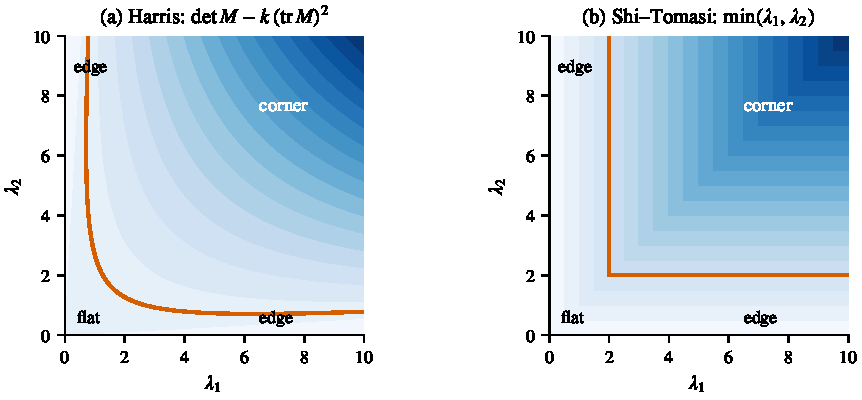
\includegraphics[width=\textwidth]{fig_structure_tensor.pdf}
  \caption{Corner scores over the plane of structure-tensor eigenvalues, with a threshold contour (orange). Both scores accept only windows with two large
  eigenvalues. Shi--Tomasi's $\min(\lambda_1, \lambda_2)$ is exactly the quantity that makes the Lucas--Kanade system well conditioned.}
  \label{fig:structure-tensor}
\end{figure}

\begin{figure}[t]
  \centering
  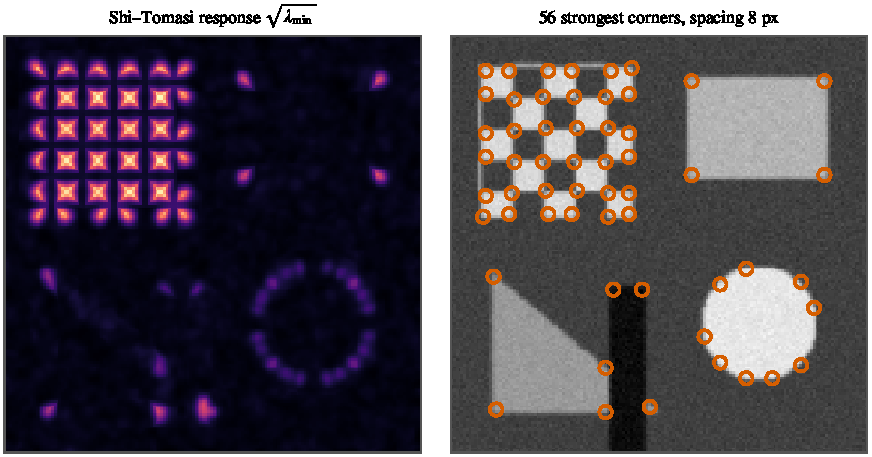
\includegraphics[width=\textwidth]{fig_harris.pdf}
  \caption{Shi--Tomasi corner response on a synthetic image (left), and the strongest corners after non-maximum suppression with a minimum spacing of 8~px (right).
  Edges and flat regions get low scores; corners and blob-like texture get high ones.}
  \label{fig:harris}
\end{figure}

Other detectors trade quality for speed. FAST classifies a pixel as a corner if a long enough arc of the 16 pixels on a circle around it is uniformly brighter or
darker than the center, using only comparisons; it is very fast but noisier. Detectors used for matching across large viewpoint changes add \emph{scale}
selection (detecting at several pyramid levels) and an \emph{orientation} for each feature, as ORB does. A frame-to-frame tracker needs neither.

% ==============================================================================
\section{Lucas--Kanade optical flow}

\subsection{Brightness constancy and the aperture problem}

Assume that a scene point keeps its brightness between consecutive frames, $I_{k+1}(x + d) = I_k(x)$, where $d$ is the image motion of the point. Linearizing in $d$,
\begin{equation}
  I_{k+1}(x) + \nabla I\T d \approx I_k(x)
  \quad\Longleftrightarrow\quad
  I_u\,d_u + I_v\,d_v + I_t = 0, \qquad I_t = I_{k+1}(x) - I_k(x).
  \label{eq:ofc}
\end{equation}
This \emph{optical-flow constraint} is one equation in two unknowns. It determines only the component of $d$ along the gradient: motion along an edge is invisible.
This is the \term{aperture problem}, the same phenomenon seen through a small hole when a long line slides past: only its perpendicular motion is visible.

\subsection{The Lucas--Kanade solution}

\index{Lucas--Kanade tracker}
Lucas and Kanade~\cite{lucas1981iterative} assume the displacement is the same for all pixels of a small window, which provides many equations for the two
unknowns, and solve \eqref{eq:ofc} for all of them in the least-squares sense:
\begin{equation}
  \min_d \sum_{x\in W}w(x)\big(\nabla I(x)\T d + I_t(x)\big)^2
  \quad\Longrightarrow\quad
  M\,d = -\sum_{x\in W}w(x)\,I_t(x)\,\nabla I(x),
  \label{eq:lk}
\end{equation}
with the structure tensor $M$ of \eqref{eq:structure-tensor} as the normal matrix (\cref{sec:least-squares}). The system is solvable and well conditioned exactly when both
eigenvalues of $M$ are large compared with the image noise: Shi and Tomasi's insight was to select features by the very criterion that makes them trackable. With
image noise of variance $\sigma_I^2$ per pixel, the covariance of the estimated displacement is approximately $\sigma_I^2M\inv$ (\cref{prop:wls-cov}), so $1/\sqrt{\lambda_2}$ measures
how precisely the worst direction is tracked.

\subsection{Iterative refinement}

\Cref{eq:lk} rests on a linearization that holds only for small $d$. The full problem, minimizing $\sum_xw(x)(I_{k+1}(x + d) - I_k(x))^2$ over $d$, is a nonlinear least-squares
problem, and Lucas--Kanade is its Gauss--Newton solution (\cref{ch:nlls}):

\begin{algorithm}[h]
\caption{Iterative Lucas--Kanade for one feature}
\label{alg:lk}
\begin{algorithmic}[1]
\Require images $I_k$, $I_{k+1}$; feature position $x_0$; initial guess $d$ (zero, or a prediction)
\State compute the template $T(x) = I_k(x)$ and its gradients over the window around $x_0$; compute $M$ and factor it
\Repeat
  \State sample $I_{k+1}(x + d)$ over the window with bilinear interpolation (\cref{sec:interpolation})
  \State $e(x) \gets I_{k+1}(x + d) - T(x)$ \Comment{residual image}
  \State solve $M\,\Delta d = -\sum_xw(x)\,e(x)\,\nabla T(x)$
  \State $d \gets d + \Delta d$
\Until{$\|\Delta d\| < 0.01$~px or the iteration limit is reached}
\end{algorithmic}
\end{algorithm}

Using the gradients of the \emph{template} $T = I_k$ rather than of the warped image lets $M$ be computed and factored once per feature (the \emph{inverse
compositional} idea, analyzed by Baker and Matthews~\cite{baker2004lk}). Sub-pixel accuracy comes from the bilinear interpolation. A few iterations usually
suffice when the initial guess is within the window radius.

\subsection{Pyramids}

The linearization is valid only for displacements smaller than the scale over which the image gradient is roughly constant, about the window radius. Fast motion
violates this: at 1~rad/s and 20~Hz, the image moves by about 23~px between frames. The remedy is a Gaussian pyramid (\cref{sec:pyramids}). Tracking starts at the
coarsest level, where a 24-pixel motion becomes a 3-pixel motion; the result, doubled, initializes the next finer level, and so on down to full resolution
(\cref{fig:pyramid})~\cite{bouguet2001pyramidal}. With $L$ levels above the base, the trackable displacement grows by about $2^L$.

\begin{figure}[t]
\centering
\begin{tikzpicture}[scale=0.9]
  \foreach \l/\s/\y in {0/3.2/0, 1/1.6/2.0, 2/0.8/3.2, 3/0.4/3.95} {
    \draw[fill=primarylight, draw=primary] (-\s, \y) -- (\s, \y) -- ({\s*0.75}, {\y + 0.35}) -- ({-\s*0.75}, {\y + 0.35}) -- cycle;
    \node[font=\footnotesize, right] at ({\s + 0.2}, {\y + 0.15}) {level \l: $\frac{1}{2^{\l}}$ resolution};
  }
  \draw[->, plotorange, thick] (-0.3,4.2) -- (-0.15,3.55) -- (0.2,2.4) -- (0.9,0.25);
  \node[plotorange, font=\footnotesize, align=right, left] at (-2.0,3.2) {coarse estimate,\\refined at each level};
\end{tikzpicture}
\caption{Pyramidal tracking. A displacement that is too large to linearize at full resolution is small at the top level; each level doubles the estimate and refines
it.}
\label{fig:pyramid}
\end{figure}

\begin{figure}[t]
  \centering
  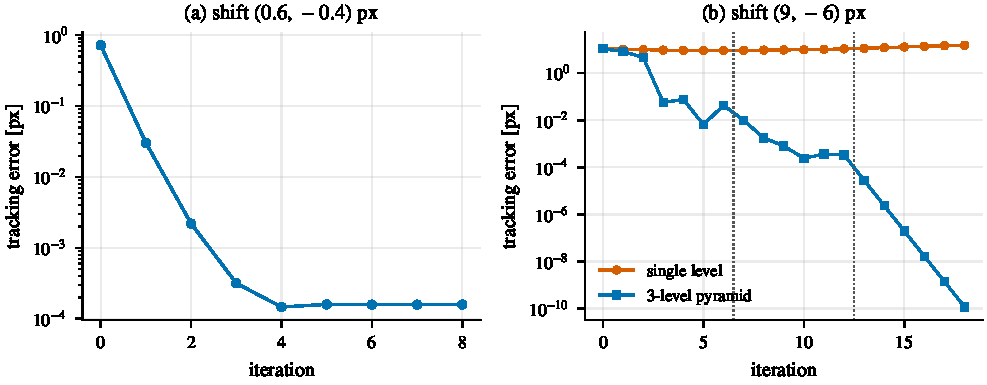
\includegraphics[width=\textwidth]{fig_lk.pdf}
  \caption{Lucas--Kanade on a synthetic textured image. (a) For a small shift of $(0.6, -0.4)$~px, the tracking error falls by orders of magnitude in a few
  Gauss--Newton iterations. (b) For a shift of $(9, -6)$~px, single-level tracking stalls in a wrong local minimum, while a three-level pyramid converges.}
  \label{fig:lk}
\end{figure}

\subsection{When tracking fails}

Lucas--Kanade fails when its assumptions fail: on edges and flat regions (an ill-conditioned $M$, the aperture problem); under occlusion, when the point disappears
behind another object; under strong brightness changes (\cref{ch:imageproc}); under motion blur, which smears the texture the tracker relies on; and when the
window straddles a depth discontinuity, where the two halves move differently. Most failures go undetected by the tracker itself, which returns a confident but wrong
position. Hence the checks of the next section.

% ==============================================================================
\section{Making tracking robust}

Optical flow optimizes photometric similarity, not physical correctness. It will track the shadow of a moving object, a specular highlight, or a T-junction formed by
two objects at different depths. Several layers of checks remove such tracks.
\begin{enumerate}
  \item \textbf{Forward-backward consistency.} Track each point from frame $k$ to $k+1$, then back to $k$. A correct track returns to its starting point; reject it if
        the round-trip error exceeds a fraction of a pixel.
  \item \textbf{IMU-aided prediction.} The gyroscope predicts the rotation between frames, $R_{c_2c_1} = R_{bc}\T R_{b_1b_2}\T R_{bc}$, where $R_{b_1b_2}$ is the integrated gyro rotation.
        For distant points, or a purely rotating camera, image points move by the infinite homography (\cref{ch:camera}): in pixels,
        $\tilde u_2 \propto KR_{c_2c_1}K\inv\tilde u_1$ (after undistortion). Starting LK from this prediction gives it a much better initial guess, and allows smaller windows and
        fewer pyramid levels.
  \item \textbf{Geometric verification.} Reject tracks that violate the epipolar constraint, with essential-matrix or two-point RANSAC, or the rotation-only constraint under
        low parallax (\cref{ch:multiview}).
  \item \textbf{Statistical gating in the filter.} Tracks that pass all of the above are still gated by the $\chi^2$ test of the MSCKF update (\cref{ch:msckfupdate}).
\end{enumerate}

\subsection{Feature distribution}

Asking a detector for the 200 strongest corners typically returns clusters on the most textured object in view. Clustered features constrain the motion poorly:
features in a small patch of the image make rotation and translation hard to separate. The standard remedy is \emph{grid bucketing}: divide the image into cells
(for example $8\times6$) and cap the number of features per cell, plus a minimum distance between features. New features are detected only in cells that have fallen
below their quota, using a mask around existing tracks. A uniform distribution of bearings makes the stacked measurement Jacobian better conditioned, which is
exactly what the estimator needs.

% ==============================================================================
\section{The feature life cycle}

\begin{figure}[h]
\centering
\begin{tikzpicture}[node distance=13mm and 34mm, every node/.style={font=\small}]
  \node[block] (new) {NEW};
  \node[block, right=of new] (trk) {TRACKED};
  \node[block, right=of trk] (lost) {LOST};
  \node[block, below=of trk, fill=white] (used) {consumed by update\\or discarded};
  \draw[->, thick] (new) -- node[above, font=\footnotesize]{tracked} (trk);
  \draw[->, thick] (trk) edge[loop above] node[above, font=\footnotesize]{tracked again} (trk);
  \draw[->, thick] (trk) -- node[above, font=\footnotesize]{track fails} (lost);
  \draw[->, thick] (lost) |- (used);
  \draw[->, thick] (trk) -- node[right, font=\footnotesize, align=left]{oldest observation's\\clone leaving the window} (used);
  \draw[->, thick] (new) |- node[left, font=\footnotesize, pos=0.25]{rejected} (used);
\end{tikzpicture}
\caption{Feature life cycle. A track is handed to the MSCKF update when it is lost, or when its oldest observation is about to leave the sliding window
(AGENTS.md F5). Its observations are used once and then discarded.}
\label{fig:lifecycle}
\end{figure}

Each feature has a persistent ID and a history of observations: (clone index or image timestamp, normalized coordinates). Since the estimator can only use
observations made at times that still have a clone in the window, the history never needs to exceed \code{kMaxClones} entries. That makes it possible to store all
tracks in a fixed-capacity pool with fixed-capacity histories, so the steady state of the front end performs no allocation for its bookkeeping (Milestone 9).

\begin{pitfall}[using a measurement twice]
Once a track's observations have been used in an MSCKF update, they must never be used again, not even partially. Re-using them double counts the same information
and makes the filter overconfident. If a track continues after being used (because its oldest clone was marginalized), its subsequent observations start a fresh
track.
\end{pitfall}

% ==============================================================================
\section{Engineering the front end}

The front end is the one component allowed to allocate (AGENTS.md E4), because OpenCV allocates internally, but it must reuse its buffers. In practice: keep the
previous pyramid and swap it with the new one instead of rebuilding storage; preallocate point vectors with \code{reserve}; keep the \code{cv::Mat} objects as members
so that their memory is reused when sizes do not change; and \emph{measure} the remaining allocations with the allocation guard rather than claiming they are zero.
Feature tracking is typically the most expensive part of the pipeline in time, too, so bucketing parameters, window size and pyramid depth are the main
performance knobs.

Descriptor-based front ends (ORB, BRIEF) describe each feature by a binary string of intensity comparisons in its neighborhood and match features across frames by
the Hamming distance between descriptors, rejecting ambiguous matches whose best and second-best distances are similar (the \emph{ratio test}). They handle large
viewpoint changes and re-detection after occlusion, which matters for loop closure, but for frame-to-frame VIO at 20~Hz KLT tracking is cheaper and more accurate.
Direct methods skip features altogether and use photometric error in the estimator itself.

\begin{projectlink}[Milestones 8 and 9]
M8 builds detection, bucketing, pyramidal LK with forward-backward checks, persistent IDs and point undistortion, and tests them on synthetic images with known
sub-pixel motion. M9 adds the life-cycle manager with a fixed-capacity pool and essential-matrix RANSAC in normalized coordinates, including the documented
pure-rotation behavior.
\end{projectlink}

\begin{takeaways}
\begin{itemize}
  \item The structure tensor $M$, from a first-order expansion of the patch auto-correlation, measures how well a window's position is defined; corners have two
        large eigenvalues.
  \item Lucas--Kanade is Gauss--Newton on the patch alignment error; its normal matrix is $M$, so good corners are exactly the trackable windows.
  \item The aperture problem: a single pixel constrains only the flow along the gradient.
  \item Pyramids extend the trackable displacement; gyro prediction makes tracking cheaper and more robust.
  \item Bucketing spreads features for good geometry; forward-backward checks and RANSAC remove bad tracks.
  \item Tracks are consumed exactly once and their histories are bounded by the window size.
\end{itemize}
\end{takeaways}

\begin{exercises}
  \item Compute the structure tensor of an ideal step edge and of an ideal corner, and verify the eigenvalue picture.
  \item Derive the closed-form smallest eigenvalue of a symmetric $2\times2$ matrix used by the Shi--Tomasi detector.
  \item Implement \cref{alg:lk} for a synthetic textured image translated by $(0.3, -0.7)$ pixels and reproduce \cref{fig:lk}(a). What happens with a translation of
        8~pixels, and how many pyramid levels fix it?
  \item Show that the forward-backward error of a correct track is due only to noise and interpolation, and estimate a sensible threshold.
  \item Compute the pixel displacement predicted by the gyroscope for a feature at the image center when the camera rotates by $0.05$~rad about its $y$-axis between frames.
  \item Implement grid bucketing and plot the feature distribution with and without it on a EuRoC image.
  \item Design the data structure for the feature pool with fixed capacity and per-feature histories bounded by \code{kMaxClones}. What happens when the pool is full?
\end{exercises}
\input{chapters/solutions/22_features_tracking}

\chapter{Multiple-View Geometry}
\label{ch:multiview}

\begin{objectives}
\begin{itemize}
  \item Derive the epipolar constraint, the essential and fundamental matrices, epipoles and epipolar lines.
  \item Recover relative motion from correspondences: the eight-point algorithm with normalization, the five-point and two-point methods, and the
        decomposition of the essential matrix.
  \item Understand homographies between views, the pure-rotation case, and the degeneracies of relative-pose estimation.
  \item Use RANSAC to reject outliers, size its iteration count, and set thresholds in the right units.
  \item Triangulate points by midpoint, linear and Gauss--Newton methods, and quantify triangulation accuracy.
  \item Understand bundle adjustment, its sparsity and its gauge freedom: the batch problem the MSCKF approximates.
\end{itemize}
\end{objectives}

% ==============================================================================
\section{Epipolar geometry}

\subsection{The epipolar constraint}

Two cameras observe the same 3D point. Let the coordinates of the point in the two camera frames be $X_1$ and $X_2$, related by the rigid motion
\begin{equation}
  X_2 = R\,X_1 + t, \qquad R = R_{c_2c_1},\quad t = p_{c_2c_1},
\end{equation}
and let $\bar x_1 = X_1/Z_1$ and $\bar x_2 = X_2/Z_2$ be the bearings (homogeneous normalized coordinates).

\begin{theorem}[Epipolar constraint]
\label{thm:epipolar}
\index{epipolar constraint}\index{essential matrix}
Every correspondence of a rigid point satisfies
\begin{equation}
  \bar x_2\T\,E\,\bar x_1 = 0, \qquad E = \sx{t}\,R .
  \label{eq:epipolar}
\end{equation}
\end{theorem}
\begin{proof}
Cross both sides of $X_2 = RX_1 + t$ with $t$: $\sx{t}X_2 = \sx{t}RX_1$. The left side is orthogonal to $X_2$, so $X_2\T\sx{t}RX_1 = 0$. Dividing by $Z_1Z_2 > 0$ gives
\eqref{eq:epipolar}.
\end{proof}

Geometrically, the two camera centers and the 3D point span a plane, the \emph{epipolar plane}, and the constraint states that the two viewing rays and the baseline
are coplanar (\cref{fig:epipolar}). The constraint involves no depth: it is a statement about bearings only, which is why it is the natural tool for checking tracks
before any 3D reconstruction exists.

\begin{figure}[t]
\centering
\begin{tikzpicture}[scale=1.0]
  \coordinate (C1) at (0,0); \coordinate (C2) at (5,0.3); \coordinate (P) at (2.7,3.4);
  \fill[primarylight, opacity=0.7] (C1) -- (C2) -- (P) -- cycle;
  \draw[thick] (C1) -- (C2) node[midway, below] {baseline $t$};
  \draw[plotgreen, thick] (C1) -- (P); \draw[plotgreen, thick] (C2) -- (P);
  \fill (C1) circle (1.8pt) node[below left] {$C_1$};
  \fill (C2) circle (1.8pt) node[below right] {$C_2$};
  \fill[conv] (P) circle (2pt) node[above] {$p_f$};
  \draw[primary, thick] (0.3,1.5) -- (1.6,1.2) -- (1.6,0.2) -- (0.3,0.5) -- cycle;
  \draw[primary, thick] (3.5,1.3) -- (4.8,1.7) -- (4.8,0.7) -- (3.5,0.3) -- cycle;
  \fill[plotgreen] ($(C1)!0.3!(P)$) circle (1.5pt) node[left, font=\footnotesize] {$\bar x_1$};
  \fill[plotgreen] ($(C2)!0.3!(P)$) circle (1.5pt) node[right, font=\footnotesize] {$\bar x_2$};
  \draw[conv, dashed] (3.6,0.65) -- (4.75,1.45);
  \node[conv, font=\footnotesize, anchor=west] at (5.0,1.25) {epipolar line $E\bar x_1$};
  \node[font=\footnotesize, primary] at (2.6,1.7) {epipolar plane};
\end{tikzpicture}
\caption{Epipolar geometry. The camera centers, the point and both viewing rays lie in one plane. The image of the point in the second camera must therefore lie on
the line where that plane cuts the second image.}
\label{fig:epipolar}
\end{figure}

\subsection{Epipolar lines and epipoles}

Given $\bar x_1$, the vector $\ell_2 = E\bar x_1$ represents a line in the second image (\cref{sec:homogeneous}), the \term{epipolar line}: the corresponding point must lie on
it. Searching for a match can be restricted to this line. All epipolar lines in the second image pass through the \term{epipole} $e_2$, the image of the first camera
center, which satisfies $e_2\T E = 0$ (it is proportional to $t$); symmetrically $Ee_1 = 0$ with $e_1 \propto R\T t$. When the camera moves forward, the epipole is the
\emph{focus of expansion} from which image points flow outward.

\begin{proposition}[Properties of the essential matrix]
\label{prop:essential}
For $t \ne 0$, $E = \sx{t}R$ has rank two and two equal non-zero singular values, $(\|t\|, \|t\|, 0)$. It has five degrees of freedom: three for the rotation and two for the
direction of $t$. Its overall scale, like the scale of $t$, is unobservable.
\end{proposition}
\begin{proof}
$EE\T = \sx{t}RR\T\sx{t}\T = -\sx{t}^2 = \|t\|^2I - tt\T$ by \eqref{eq:skew-sq}, whose eigenvalues are $\|t\|^2$ (twice, on the plane orthogonal to $t$) and $0$ (along $t$). The
singular values of $E$ are their square roots.
\end{proof}

In pixel coordinates, with $\tilde u_i = K\bar x_i$, the constraint reads $\tilde u_2\T F\tilde u_1 = 0$ with the \term{fundamental matrix} $F = K\mT EK\inv$ (seven degrees of freedom,
rank two). The project works with undistorted normalized coordinates throughout, so it uses $E$ directly (Milestone 9).

% ==============================================================================
\section{Estimating relative motion}

\subsection{The eight-point algorithm}

\Cref{eq:epipolar} is linear in the nine entries of $E$. Writing $\bar x_1 = (x_1, y_1, 1)$ and $\bar x_2 = (x_2, y_2, 1)$, each correspondence gives one equation
\begin{equation}
  a\T e = 0, \qquad a = (x_2x_1,\ x_2y_1,\ x_2,\ y_2x_1,\ y_2y_1,\ y_2,\ x_1,\ y_1,\ 1), \qquad e = \vect_{\text{rows}}(E).
\end{equation}
With eight or more correspondences, stack them into $Ae = 0$ and take the unit vector minimizing $\|Ae\|$: the right singular vector of $A$ with the smallest
singular value (\cref{prop:homogeneous-ls}). Noise makes the result an invalid essential matrix, which is projected onto the nearest valid one by replacing its
singular values with $(1, 1, 0)$ (\cref{thm:svd} and Eckart--Young). When the algorithm is applied to pixel coordinates (to estimate $F$), the coordinates must first
be \emph{normalized} (translated to zero mean and scaled to unit average distance from the origin), or the matrix $A$, whose entries range from 1 to $10^5$, is so
badly conditioned that the result is unusable; this is Hartley's normalization.

\subsection{Decomposing the essential matrix}

\begin{proposition}[Motion from the essential matrix]
\label{prop:e-decomposition}
Let $E = U\diag(1, 1, 0)V\T$ with $U, V$ rotations (flip their signs if needed), and $W = \begin{bmatrix}0 & -1 & 0\\ 1 & 0 & 0\\ 0 & 0 & 1\end{bmatrix}$. The rotation and translation
direction are one of the four combinations
\begin{equation}
  R \in \{UWV\T,\ UW\T V\T\}, \qquad t \in \{+u_3,\ -u_3\},
\end{equation}
where $u_3$ is the third column of $U$. Exactly one of the four places triangulated points in front of both cameras.
\end{proposition}

The proof checks that $\sx{u_3}UWV\T$ and $\sx{u_3}UW\T V\T$ both equal $E$ up to sign, and that no other factorizations exist. The four solutions correspond to the second
camera being on either side of the first, facing either forward or backward; the \emph{cheirality} test (positive depth of a triangulated point in both views)
selects the physical one.

\subsection{The five-point and two-point methods}

Five correspondences are the minimum, since $E$ has five degrees of freedom. Nistér's algorithm~\cite{nister2004five} combines the linear constraints of five
correspondences with the cubic constraints that characterize essential matrices ($\det E = 0$ and $2EE\T E - \tr(EE\T)E = 0$) and solves the resulting polynomial system,
returning up to ten candidates. Fewer points per hypothesis means fewer RANSAC iterations, which is why \code{cv::findEssentialMat} uses it.

In VIO the gyroscope supplies the relative rotation $R$ between consecutive frames with high accuracy. With $R$ known, \eqref{eq:epipolar} becomes linear in $t$:
\begin{equation}
  \bar x_2\T\sx{t}R\bar x_1 = t\T\big(R\bar x_1\times\bar x_2\big) = 0 .
\end{equation}
Each correspondence says that $t$ is orthogonal to the vector $c_i = R\bar x_1^{(i)}\times\bar x_2^{(i)}$, so two correspondences determine the direction of $t$ as $c_1\times c_2$. A two-point
hypothesis needs far fewer RANSAC iterations than a five-point one, and it is the outlier-rejection strategy of MSCKF-VIO~\cite{sun2018msckfvio}.

\subsection{Measuring the residual}

The algebraic residual $\bar x_2\T E\bar x_1$ has no geometric meaning. The geometric error of a correspondence is the smallest displacement of $\bar x_1$ and $\bar x_2$ that
makes the constraint hold exactly. Linearizing the constraint in that displacement gives the \emph{Sampson distance}
\begin{equation}
  d_S = \frac{(\bar x_2\T E\bar x_1)^2}{(E\bar x_1)_1^2 + (E\bar x_1)_2^2 + (E\T\bar x_2)_1^2 + (E\T\bar x_2)_2^2},
\end{equation}
the squared residual divided by the squared norm of its gradient with respect to the four image coordinates: the first-order squared distance to the constraint
surface. It is in the units of the coordinates used. With normalized coordinates, a pixel threshold $\tau_{px}$ must be converted to $\tau_{px}/f$ (Milestone 9).

\begin{pitfall}[thresholds in the wrong units]
Calling \code{cv::findEssentialMat} on normalized coordinates with an identity camera matrix and a threshold of ``1.0'' accepts residuals of 1 normalized unit, about
450 pixels: every track becomes an inlier. The threshold must be $\tau_{px}/f$, e.g.\ $1/458 \approx 2.2\times10^{-3}$.
\end{pitfall}

% ==============================================================================
\section{Homographies between views}
\label{sec:homographies}

\paragraph{Planar scenes.} If all points lie on a plane $n\T X_1 = d$ (unit normal $n$ and distance $d$ in the first camera's frame), then $1 = n\T X_1/d$ and
$X_2 = RX_1 + t\,n\T X_1/d$, so
\begin{equation}
  X_2 = \Big(R + \frac{t\,n\T}{d}\Big)X_1, \qquad \bar x_2 \propto H\bar x_1, \quad H = R + \frac{tn\T}{d} .
\end{equation}
\paragraph{Pure rotation.} If $t = 0$, $X_2 = RX_1$ for every point, at any depth: $\bar x_2 \propto R\bar x_1$, the \emph{infinite homography}. In pixels it is $KRK\inv$.

A homography has eight degrees of freedom and is estimated from four or more correspondences by a direct linear transform: each correspondence gives two linear
equations in the nine entries of $H$ (from $\tilde x_2\times H\tilde x_1 = 0$), solved by \cref{prop:homogeneous-ls}.

% ==============================================================================
\section{RANSAC}

Random Sample Consensus~\cite{fischler1981ransac} estimates a model from data containing outliers by hypothesis and verification.

\begin{algorithm}[h]
\caption{RANSAC}
\begin{algorithmic}[1]
\Require data, minimal sample size $s$, threshold $\tau$, confidence $p$
\State best $\gets \emptyset$; $N \gets \infty$; $k \gets 0$
\While{$k < N$}
  \State draw $s$ data points at random; fit candidate models
  \State count inliers with residual $< \tau$; keep the model with the most inliers
  \State update $N$ from the current inlier ratio $w$ with \eqref{eq:ransac-n}; $k \gets k + 1$
\EndWhile
\State refit the model on all inliers of the best hypothesis (least squares)
\end{algorithmic}
\end{algorithm}

If a fraction $w$ of the data are inliers, a random minimal sample is outlier-free with probability $w^s$, and $N$ independent samples all contain an outlier with probability
$(1 - w^s)^N$. Requiring this to be at most $1 - p$ gives the number of iterations
\begin{equation}
  N = \frac{\log(1 - p)}{\log(1 - w^s)} .
  \label{eq:ransac-n}
\end{equation}
\begin{center}\small
\begin{tabular}{@{}l c c c@{}}
\toprule
$p = 0.99$ & $w = 0.9$ & $w = 0.7$ & $w = 0.5$ \\
\midrule
8-point ($s = 8$) & 9 & 78 & 1177 \\
5-point ($s = 5$) & 6 & 26 & 146 \\
2-point ($s = 2$) & 3 & 7 & 17 \\
\bottomrule
\end{tabular}
\end{center}
The exponential dependence on $s$ is why minimal solvers matter, and why using the gyroscope to remove three unknowns pays off. Since $w$ is unknown in advance, the
algorithm starts pessimistic and updates $N$ from the best inlier ratio found so far (adaptive termination). Variants score hypotheses by the sum of truncated
residuals (MSAC) rather than the inlier count, or refine the best hypothesis locally (LO-RANSAC).

\begin{figure}[t]
  \centering
  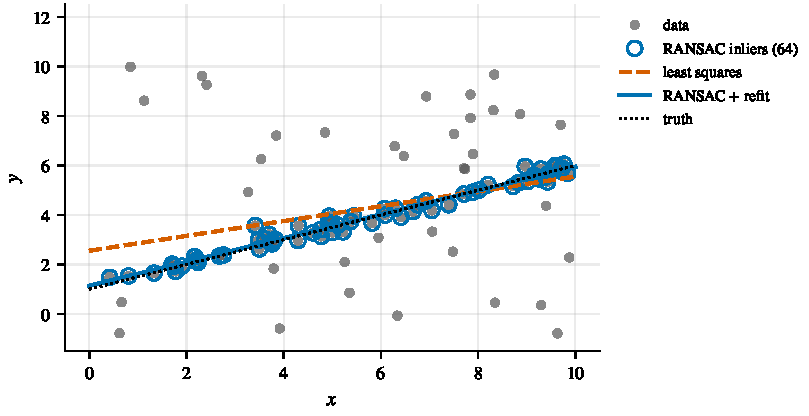
\includegraphics[width=0.86\textwidth]{fig_ransac.pdf}
  \caption{Fitting a line to data with 40\% gross outliers. Least squares is dragged away by the outliers; RANSAC finds the line supported by the most inliers
  (circled) and refits it to them.}
  \label{fig:ransac}
\end{figure}

% ==============================================================================
\section{Degeneracies}

\subsection{Pure rotation}

If the camera only rotates, $t = 0$ and $E = \sx{0}R = 0$: the epipolar constraint is satisfied by every pair of points, inlier or not. Under small translation the problem is
not degenerate but badly conditioned: $t$ is poorly determined, inlier sets fluctuate, and RANSAC may reject good tracks or accept bad ones. Hovering drones rotate in
place often, so this case must be handled (Milestone 9).

Under pure rotation the correspondences satisfy the stronger constraint $\bar x_2 \propto R\bar x_1$ (\cref{sec:homographies}), which does not involve $t$ at all. A robust front end
measures the parallax remaining after rotation compensation, for example the median of $\|\pi(R\bar x_1) - \pi(\bar x_2)\|$ over the tracks:
\begin{itemize}
  \item if it is large, run essential-matrix (or two-point) RANSAC;
  \item if it is tiny, skip epipolar RANSAC and reject only tracks that violate the rotation-only prediction $\bar x_2 \propto R\bar x_1$, with $R$ from the gyroscope.
\end{itemize}
Either way the system keeps tracking: low parallax means the features carry little information about translation, not that they are wrong. The MSCKF update
handles them gracefully, because their nullspace-projected residuals simply contribute little.

\subsection{Other degeneracies}

The eight-point algorithm is degenerate when all points lie on a plane, a common situation (floors, walls), because a homography then explains the data equally well;
the five-point algorithm is not. Very distant points behave like points at infinity and carry only rotational information. Moving objects form a second, consistent
rigid motion that RANSAC can mistake for the dominant one if they fill the image.

% ==============================================================================
\section{Triangulation}
\label{sec:triangulation}

Given observations $z_i$ of a point in cameras with known poses $(R_{wc_i}, p_{wc_i})$, triangulation estimates its world position $p_f$.

\subsection{The midpoint method}

Each observation defines a ray $p_{wc_i} + \lambda_ir_i$ with direction $r_i = R_{wc_i}\bar x_i$. With noise the rays do not intersect. The midpoint method finds the point
closest to all rays in the least-squares sense: the distance of $p$ from ray $i$ is $\|(I - \hat r_i\hat r_i\T)(p - p_{wc_i})\|$ with $\hat r_i$ the unit direction, so
\begin{equation}
  \Big(\sum_i(I - \hat r_i\hat r_i\T)\Big)\,p = \sum_i(I - \hat r_i\hat r_i\T)\,p_{wc_i} .
\end{equation}
It is simple and geometric, but it minimizes 3D distances rather than image errors, which weights distant views wrongly.

\subsection{Linear triangulation}

In camera $i$ the point has coordinates $X_i = R_{wc_i}\T(p_f - p_{wc_i})$, which must be parallel to the bearing $\bar x_i = (z_i, 1)$: $\sx{\bar x_i}X_i = 0$. Substituting,
\begin{equation}
  \sx{\bar x_i}R_{wc_i}\T\, p_f = \sx{\bar x_i}R_{wc_i}\T\, p_{wc_i}, \qquad i = 1,\dots,M .
  \label{eq:dlt}
\end{equation}
Each view contributes three equations of rank two. Stacking all views gives an overdetermined linear system $A p_f = b$ that is solved in the least-squares sense with
QR or SVD. With two views and noise-free data the solution is exact. This is the linear initialization of AGENTS.md F5. It minimizes an algebraic error, not the
reprojection error, so it is refined next.

\subsection{Nonlinear refinement with inverse depth}

The maximum-likelihood estimate minimizes the reprojection error (\cref{ch:nlls})
\begin{equation}
  \min_{p_f}\ \sum_{i=1}^M \big\| z_i - \pi(X_i(p_f)) \big\|^2 .
\end{equation}
The MSCKF~\cite{mourikis2007msckf} parameterizes the point in an \emph{anchor} camera $A$ (for example the first observation) by inverse depth~\cite{civera2008inverse}:
\begin{equation}
  X_A = \frac1\rho\begin{bmatrix} \alpha \\ \beta \\ 1 \end{bmatrix}, \qquad
  X_i = R_{iA}X_A + p_{iA}
  \quad\Longrightarrow\quad
  h_i := \rho X_i = R_{iA}\begin{bmatrix}\alpha\\ \beta\\ 1\end{bmatrix} + \rho\,p_{iA}, \quad z_i = \pi(h_i),
\end{equation}
where $(R_{iA}, p_{iA})$ is the transformation from the anchor camera to camera $i$, computed from the clone poses, and $\pi(h_i) = \pi(X_i)$ because projection ignores scale.
The parameters $(\alpha, \beta)$ are the normalized coordinates in the anchor view and $\rho = 1/Z_A$ is the inverse depth. This parameterization behaves well for distant points
($\rho\to0$ is a regular point), and the measurement function is nearly linear in $(\alpha, \beta, \rho)$. Its Jacobian follows from the chain rule:
\begin{equation}
  \frac{\partial z_i}{\partial(\alpha, \beta, \rho)} = \frac{\partial\pi}{\partial h}\Big|_{h_i}\,
  \begin{bmatrix} r_1 & r_2 & p_{iA} \end{bmatrix},
\end{equation}
where $r_1, r_2$ are the first two columns of $R_{iA}$ and $\partial\pi/\partial h$ is \cref{prop:proj-jacobian}. Gauss--Newton (\cref{alg:gauss-newton}) iterates
$\delta y = -(J\T J)\inv J\T e$ with the stacked Jacobian $J$ and residual $e$, usually converging in a few iterations from the linear initialization. Levenberg--Marquardt
damping adds robustness.

\subsection{How accurate is triangulation?}

For two views separated by a baseline $b$ perpendicular to the viewing direction, the depth is $Z = b/d$ with $d$ the disparity in normalized coordinates. With
independent noise $\sigma_{uv}$ in each view, $\sigma_d = \sqrt2\sigma_{uv}$, and since $\partial Z/\partial d = -b/d^2 = -Z^2/b$, to first order
\begin{equation}
  \sigma_Z \approx \frac{Z^2}{b}\sqrt2\,\sigma_{uv} .
  \label{eq:depth-sigma}
\end{equation}
Depth error grows quadratically with depth and inversely with baseline. Equivalently, the relative depth error is inversely proportional to the parallax angle $\approx b/Z$.

\begin{figure}[t]
  \centering
  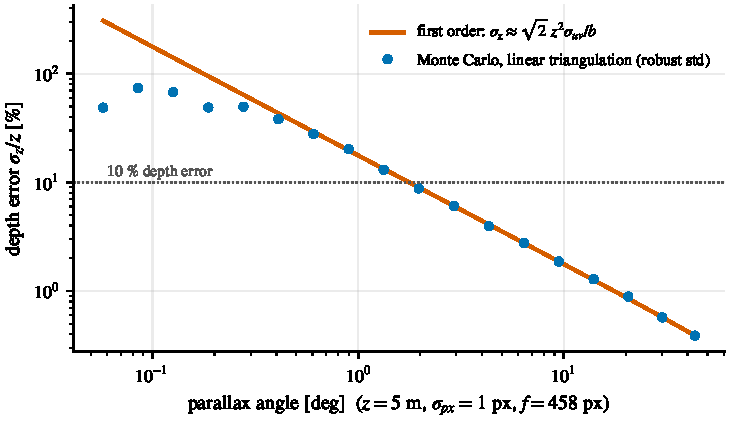
\includegraphics[width=0.86\textwidth]{fig_triangulation.pdf}
  \caption{Relative depth error of two-view triangulation at $Z = 5$~m with 1-pixel noise, versus parallax angle. Down to about $1^\circ$ the first-order formula \eqref{eq:depth-sigma}
  describes the spread accurately. Below that the error distribution becomes heavy-tailed (depths can even become negative), and the estimate is unusable.}
  \label{fig:triangulation}
\end{figure}

\Cref{fig:triangulation} shows that 10\% depth accuracy needs about $2^\circ$ of parallax, a baseline of 17~cm at 5~m. Down to about $1^\circ$ \eqref{eq:depth-sigma} still
describes the bulk of the estimates; below that, outliers take over. At $0.5^\circ$, 4\% of the estimates are off by more than five standard deviations, and at
$0.25^\circ$, 8\% of the depths come out negative. A triangulation module must therefore check its own result before handing it to the filter:
\begin{itemize}
  \item positive depth in every view (cheirality);
  \item sufficient parallax (or baseline relative to depth), or equivalently a well-conditioned Gauss--Newton Hessian;
  \item small reprojection error in every view after refinement;
  \item a plausible depth range.
\end{itemize}
Features that fail are discarded, not fed to the update (AGENTS.md F5, Milestone 10b).

% ==============================================================================
\section{Bundle adjustment}
\label{sec:bundle-adjustment}

\termi{Bundle adjustment}{bundle adjustment} estimates all camera poses and all 3D points at once by minimizing the total reprojection error,
\begin{equation}
  \min_{\{T_i\},\{p_j\}}\ \sum_{(i,j)\text{ observed}}\big\|z_{ij} - \pi\big(T_i\inv p_j\big)\big\|^2_{R\inv},
\end{equation}
with Gauss--Newton or Levenberg--Marquardt on the manifold of poses (\cref{ch:nlls}). It is the gold standard of geometric vision. Two of its properties illuminate
VIO.
\begin{itemize}
  \item \emph{Structure.} Each residual involves one camera and one point, so the normal equations have the block structure of \cref{sec:schur-ba}: eliminating the
        points with the Schur complement leaves a small \emph{reduced camera system} (\cref{fig:ba-sparsity}).
  \item \emph{Gauge freedom.} Moving and rotating everything together, or (for a monocular camera) scaling everything, leaves all reprojection errors unchanged: the
        problem has seven unobservable directions, and $J\T WJ$ is singular along them. Solvers fix the gauge by holding the first camera fixed and the scale constant, or
        by adding a weak prior. With an IMU, scale and two rotation directions (roll and pitch) become observable, and the gauge shrinks to the four directions of
        \cref{ch:observability}.
\end{itemize}
The MSCKF can be understood as a fast, filtered approximation of bundle adjustment over a sliding window: it eliminates each point exactly as the Schur complement
does (\cref{ch:msckfupdate}), takes a single Gauss--Newton step, and summarizes the past by the filter's Gaussian prior instead of relinearizing it.

\paragraph{Pose from known points.} Finally, when the 3D points are known (a map), a single image determines the camera pose: the
\emph{perspective-$n$-point} (PnP) problem, solved minimally from three points and refined by Gauss--Newton. It is the core of relocalization against a map, a
capability that odometry lacks.

\begin{takeaways}
\begin{itemize}
  \item Rigid correspondences satisfy $\bar x_2\T\sx{t}R\bar x_1 = 0$; $E$ has 5 DOF, singular values $(\|t\|, \|t\|, 0)$, and an unobservable scale.
  \item The eight-point algorithm is linear (normalize pixel coordinates first); $E$ decomposes into four motions, one of which passes the cheirality test.
  \item With the rotation from the gyroscope, two correspondences determine the translation direction.
  \item Planes and pure rotations relate views by homographies; under pure rotation $E$ vanishes and the rotation-only constraint takes over.
  \item RANSAC iterations grow as $w^{-s}$: prefer minimal solvers. Thresholds in normalized units are $\tau_{px}/f$.
  \item Triangulate linearly, refine by Gauss--Newton with inverse depth, and reject low-parallax or negative-depth points; depth error grows as $Z^2/b$.
  \item Bundle adjustment is the batch problem; the MSCKF approximates it with exact landmark elimination and a single Gauss--Newton step.
\end{itemize}
\end{takeaways}

\begin{exercises}
  \item Verify \cref{thm:epipolar} numerically for random points and a random relative pose, then show that adding an outlier breaks it.
  \item Prove \cref{prop:essential} and show that $e_2 \propto t$ is the left null vector of $E$.
  \item Implement the eight-point algorithm with and without Hartley normalization on pixel coordinates, and compare the errors.
  \item Implement the decomposition of \cref{prop:e-decomposition} and the cheirality test, and verify on synthetic data that the correct solution is selected.
  \item Implement the two-point method with known rotation inside RANSAC on synthetic data with 30\% outliers. Compare the number of iterations needed with the five-point
        method.
  \item Generate a pure-rotation sequence, observe what \code{cv::findEssentialMat} returns, and implement the parallax test.
  \item Show that \eqref{eq:dlt} has rank two per view and that two views with non-parallel rays give a unique solution.
  \item Derive \eqref{eq:depth-sigma}, reproduce \cref{fig:triangulation}, and repeat with three views over the same baseline.
  \item Count the gauge freedoms of monocular bundle adjustment and of visual-inertial bundle adjustment, and explain the difference.
\end{exercises}
\input{chapters/solutions/23_multiview}


\part{The Multi-State Constraint Kalman Filter}
\chapter{From EKF-SLAM to the MSCKF}
\label{ch:msckfintro}

\begin{objectives}
\begin{itemize}
  \item Understand how EKF-SLAM uses visual landmarks, and why it scales poorly.
  \item Understand the central idea of the MSCKF: constraints between multiple past poses instead of landmarks.
  \item See why past poses must be kept in the state, with their correlations.
  \item Relate the MSCKF to sliding-window optimization.
\end{itemize}
\end{objectives}

% ------------------------------------------------------------------------------
\section{EKF-SLAM}

\index{EKF-SLAM}
The most direct way to use a camera in an EKF is to put the landmarks in the state. With $L$ landmarks,
\begin{equation}
  x = \big(x_I,\ p_{f_1},\ \dots,\ p_{f_L}\big), \qquad \dim\delta x = 15 + 3L,
\end{equation}
and each image observation $z = \pi(p_c(x_I, p_{f_j})) + n$ is an ordinary EKF measurement of the IMU state and one
landmark. This is EKF-SLAM, and MonoSLAM~\cite{davison2007monoslam} showed it can run in real time with a single camera.

\subsection{How it works}

\paragraph{Prediction.} Landmarks are static, so only the IMU block is propagated: exactly the block structure of clones in \cref{ch:errordyn},
$P_{II} \gets \Phi P_{II}\Phi\T + Q_d$, $P_{IL} \gets \Phi P_{IL}$, with the landmark block unchanged.

\paragraph{Update.} An observation of landmark $j$ has a Jacobian with two non-zero blocks: one for the IMU pose and one for landmark $j$,
$H = [H_I\ \ 0\ \cdots\ 0\ \ H_{f_j}\ \ 0\ \cdots]$. The gain $K = PH\T S\inv$ is nevertheless dense: every landmark correlated with the robot or with landmark $j$ is corrected.
This is how EKF-SLAM ``closes loops'': re-observing an old landmark corrects the robot, which through the correlations corrects every other landmark. It is also
what makes it expensive.

\paragraph{Landmark initialization.} A new landmark enters the state as a function of the current state and the first measurement, $p_f = g(x_I, z)$. This is the
state augmentation of \cref{prop:augmentation}: $P \gets JPJ\T + J_zRJ_z\T$ with $J = [I;\ \partial g/\partial x]$ and $J_z = [0;\ \partial g/\partial z]$. For a monocular camera, $g$
needs a depth that a single measurement does not provide, which leads to the initialization problem below.

\subsection{Why it scales poorly}

EKF-SLAM has three structural problems.
\begin{enumerate}
  \item \textbf{Cost.} The covariance has $(15 + 3L)^2$ entries, and every update touches all of them: the Joseph update costs $\mathcal{O}(n^2)$ per scalar measurement at
        best. Tracking 200 landmarks gives a $615\times615$ covariance; updating it at 20~Hz with hundreds of observations per frame is expensive, and the cost
        grows quadratically with the map.
  \item \textbf{Initialization.} A single monocular observation says nothing about depth. A new landmark must be
        initialized with a huge depth uncertainty, which is highly non-Gaussian in Euclidean coordinates, or its
        initialization must be delayed until it has been seen from several viewpoints. Inverse-depth
        parameterizations~\cite{civera2008inverse} help, but add complexity.
  \item \textbf{Housekeeping.} Landmarks that leave the field of view must either stay in the state, growing it, or be
        marginalized, which in covariance form is cheap but discards their future value.
\end{enumerate}

% ------------------------------------------------------------------------------
\section{The multi-state constraint}
\index{multi-state constraint}\index{MSCKF}

Consider a feature observed in $M$ images taken at times $t_1, \dots, t_M$. Each observation constrains the pose at its
time and the feature position. Taken together, after the unknown feature position is eliminated, the $2M$ observations
impose $2M - 3$ constraints \emph{on the $M$ poses alone}. This is the \emph{multi-state constraint}: geometric information
about how the camera moved between the images, with the scene point serving only as an intermediary.

\begin{keyidea}[the MSCKF in one sentence]
Keep a sliding window of past poses in the state instead of landmarks; when a feature track is complete,
triangulate it, linearize its observations, and eliminate the feature by projecting onto the left nullspace of its
Jacobian, leaving a residual that depends only on the poses; then update.
\end{keyidea}

Mourikis and Roumeliotis~\cite{mourikis2007msckf} showed that this uses all the information that the observations carry about
the poses (under linearization), at a cost linear in the number of features. Feature positions are never part of the
state, so there is no landmark initialization problem inside the filter, and features leaving the view simply trigger an
update.

\section{Why past poses must be in the state}

Why not keep only the current IMU state and use the constraint between the current pose and the past ones? Because the
past poses are \emph{estimated} quantities, with errors correlated with the current state's error: they were all produced by
the same propagation from the same measurements. A measurement relating the current pose to a past pose estimate, which
treats that past estimate as fixed or independent, double counts information and makes the filter overconfident.

The cure is \emph{stochastic cloning}~\cite{roumeliotis2002cloning}. When an image is captured, a copy of the current pose (a
clone) is appended to the state, together with its exact correlations to everything else. From then on the clone is a
state variable whose estimate can be corrected by later measurements, and whose correlation with the evolving IMU state is
propagated exactly. \Cref{ch:cloning} develops this in detail.

\begin{figure}[t]
\centering
\begin{tikzpicture}[scale=1.0]
  % trajectory
  \draw[->, thick, black!50] (-0.5,-0.2) .. controls (2,0.6) and (5,0.7) .. (9.4,0.1) node[right, font=\footnotesize] {time};
  % clones
  \foreach \x/\y/\a/\n in {0.3/0.02/12/1, 1.8/0.33/9/2, 3.3/0.5/5/3, 4.8/0.56/0/4, 6.3/0.5/-5/5, 7.8/0.33/-10/6} {
    \begin{scope}[shift={(\x,\y)}, rotate=\a]
      \draw[fill=primarylight, draw=primary] (-0.2,0) -- (0.2,0) -- (0.3,0.42) -- (-0.3,0.42) -- cycle;
    \end{scope}
    \node[font=\scriptsize, below=2pt] at (\x,\y) {$C_\n$};
  }
  % current IMU
  \fill[conv] (9.0,0.15) circle (2.5pt) node[below=3pt, font=\scriptsize] {IMU state};
  % features
  \coordinate (F1) at (2.4,3.2); \coordinate (F2) at (5.6,3.6); \coordinate (F3) at (7.6,2.9);
  \fill[plotgreen] (F1) circle (2.3pt) node[above] {\footnotesize $f_1$};
  \fill[plotgreen] (F2) circle (2.3pt) node[above] {\footnotesize $f_2$};
  \fill[plotgreen] (F3) circle (2.3pt) node[above] {\footnotesize $f_3$};
  \foreach \x/\y in {0.3/0.44, 1.8/0.75, 3.3/0.92} \draw[plotgreen, dashed] (\x,\y) -- (F1);
  \foreach \x/\y in {3.3/0.92, 4.8/0.98, 6.3/0.92, 7.8/0.75} \draw[plotgreen!60!black, dashed] (\x,\y) -- (F2);
  \foreach \x/\y in {6.3/0.92, 7.8/0.75} \draw[plotorange, dashed] (\x,\y) -- (F3);
  \draw[decorate, decoration={brace, amplitude=5pt, mirror}] (0,-0.55) -- (8.1,-0.55) node[midway, below=6pt, font=\footnotesize] {sliding window of $N$ clones (poses at image times), all in the state};
\end{tikzpicture}
\caption{The MSCKF state: the current IMU state plus clones of past camera poses. Feature $f_1$ is seen by clones 1--3
and constrains them; $f_2$ by clones 3--6. Neither feature is in the state. Feature $f_3$ has only two observations so far
and keeps being tracked.}
\label{fig:msckf-window}
\end{figure}

% ------------------------------------------------------------------------------
\section{The MSCKF state}

The project's state (AGENTS.md C3) is the IMU state plus $N \le$ \code{kMaxClones} clones, each holding the IMU pose
$(p_{wb}, q_{wb})$ at an image timestamp:
\begin{equation}
  x = \big(\,p,\ v,\ q,\ b_a,\ b_g,\ \ p_1, q_1,\ \dots,\ p_N, q_N\,\big),\qquad \dim\delta x = 15 + 6N .
\end{equation}
The camera pose of clone $i$ is derived through the fixed extrinsics,
$R_{wc_i} = R_{wb_i}R_{bc}$ and $p_{wc_i} = p_{wb_i} + R_{wb_i}p_{bc}$. With \code{kMaxClones} $= 10$, the error state has 75
dimensions, independent of how many features are tracked.

% ------------------------------------------------------------------------------
\section{Relation to sliding-window optimization}

Optimization-based VIO (OKVIS~\cite{leutenegger2015okvis}, VINS-Mono~\cite{qin2018vins}) keeps a similar window of poses and
minimizes the sum of squared reprojection and IMU residuals over poses \emph{and} landmarks, relinearizing at every
iteration, then marginalizes old states into a Gaussian prior. The MSCKF update is equivalent to a single Gauss--Newton
iteration of such a problem, with the landmarks eliminated by a Schur complement and the prior given by the filter's
covariance. Eliminating a landmark by nullspace projection and by Schur complement give the same information about the
poses (\cref{thm:nullspace-optimal}). The differences are that the MSCKF never relinearizes past measurements, and
processes each feature track exactly once, which makes it cheaper and more predictable, at some cost in accuracy under
strong nonlinearity.

\section{Variants}

The basic MSCKF has been refined in many directions. MSCKF 2.0~\cite{li2013msckf2} added First-Estimates Jacobians for
consistency and online calibration of extrinsics and time offset. Hybrid filters keep long-lived features in the state as
SLAM landmarks while processing short tracks MSCKF-style. MSCKF-VIO~\cite{sun2018msckfvio} uses a stereo camera and
two-point RANSAC for fast flight, and OpenVINS~\cite{geneva2020openvins} is a modular research platform that implements most of
these options and documents them carefully.

\begin{takeaways}
\begin{itemize}
  \item EKF-SLAM keeps landmarks in the state; its cost grows quadratically with the map.
  \item The MSCKF keeps past poses (clones) instead; each feature track is turned into constraints on those poses.
  \item Past poses must be in the state, with their correlations, or information is double counted.
  \item The MSCKF update is equivalent to one Gauss--Newton step of sliding-window bundle adjustment with landmarks
        marginalized.
\end{itemize}
\end{takeaways}

\begin{exercises}
  \item Estimate the memory and the per-update flop count of EKF-SLAM with 200 landmarks and of the MSCKF with 10 clones.
  \item A feature is observed in $M$ images. How many scalar constraints does it impose on the poses? Why does the count
        start being useful only at $M = 2$, and why does the project require $M \ge 3$?
  \item Explain in your own words why using a past pose estimate as if it were known exactly makes the filter
        overconfident. Construct a scalar example.
\end{exercises}

\chapter{Stochastic Cloning and the Sliding Window}
\label{ch:cloning}
\chaptermark{Stochastic Cloning} % short running header

\begin{objectives}
\begin{itemize}
  \item See, on a scalar example, why relative measurements require cloned states with correlations.
  \item Derive the general state-augmentation formula $P \gets JPJ\T$.
  \item Derive the project's cloning Jacobian and the invariance property of cloning.
  \item Marginalize the oldest clone in place without allocation, and choose a window policy and size.
\end{itemize}
\end{objectives}

% ------------------------------------------------------------------------------
\section{A scalar example}

Let $x$ be a scalar position that performs a random walk, $x_{k+1} = x_k + w_k$ with $\Var(w_k) = Q$, and suppose its
current estimate has variance $P$. At time 1 we \emph{clone} it, $x_c := x_1$; between times 1 and 2 the state moves; then a
sensor measures the displacement:
\begin{equation}
  z = x_2 - x_c + n, \qquad \Var(n) = R .
\end{equation}
Augmenting the state with the clone gives the vector $(x, x_c)$. At the moment of cloning both entries are the \emph{same}
random variable, so their joint covariance is $\begin{bmatrix} P & P \\ P & P\end{bmatrix}$, which is singular. Propagating $x$ but
not $x_c$ gives
\begin{equation}
  P_{\mathrm{aug}} = \begin{bmatrix} P + Q & P \\ P & P \end{bmatrix}, \qquad H = \begin{bmatrix} 1 & -1 \end{bmatrix}.
\end{equation}
The innovation covariance and gain are
\begin{equation}
  S = (P + Q) - 2P + P + R = Q + R, \qquad K = \frac{1}{Q + R}\begin{bmatrix} Q \\ 0 \end{bmatrix}.
\end{equation}
The result is exactly right: a displacement measurement is informative only about what happened \emph{between} the two
times, so $S$ involves only $Q$ and $R$. The update corrects the current state by the part of its uncertainty that arose
after the clone, and leaves the clone untouched. The posterior variance of $x_2$ is $P + Q - Q^2/(Q + R)$, which stays
large if $P$ is large, as it must: a relative measurement cannot reveal absolute position.

Now suppose we had treated the past estimate as known (no clone, zero variance). Then $S = P + Q + R$ and the posterior
variance of $x_2$ would be $(P + Q)R/(P + Q + R)$, which tends to $R$ when $P$ is large. The filter would believe it had
learned the absolute position to within the sensor noise from a displacement measurement: a severe overconfidence.
Treating the past estimate as an independent random variable is wrong in a different way. Only the exact
cross-covariance gives the right answer, and stochastic cloning~\cite{roumeliotis2002cloning} is the mechanism that keeps it.

% ------------------------------------------------------------------------------
\section{State augmentation}

\begin{proposition}[Augmentation with a function of the state]
\label{prop:augmentation}
Let $x$ have error covariance $P$, and append a new variable $y = g(x)$ whose error satisfies $\delta y \approx J_g\,\delta x$. The
augmented error $(\delta x, \delta y) = J\,\delta x$ with $J = \begin{bmatrix} I \\ J_g\end{bmatrix}$ has covariance
\begin{equation}
  P \gets J P J\T = \begin{bmatrix} P & PJ_g\T \\ J_gP & J_gPJ_g\T \end{bmatrix}.
  \label{eq:augmentation}
\end{equation}
\end{proposition}
\begin{proof}
\Cref{prop:affine} with the linear map $J$.
\end{proof}

The augmented covariance has rank $\dim x$: it is singular, because $y$ is a deterministic function of $x$ at the moment of
augmentation. This is correct and harmless. Propagation adds process noise to the IMU block only, after which the clone and
the current state are no longer perfectly correlated. The Joseph form and symmetrization keep the matrix positive
semi-definite throughout.

\section{The project's clone}

At an image timestamp, after propagating the IMU state to exactly that time, the filter appends a clone holding the current
pose $(p_{wb}, q_{wb})$, and augments the covariance with the cloning Jacobian (AGENTS.md F5).

\begin{derivex}{the cloning Jacobian $J$}{sol:clone}
The clone's error is defined with the same retraction as the IMU pose (AGENTS.md C4): $p_c = \hat p_c + \delta p_c$ and
$q_c = \hat q_c\qprod\Exp_q(\delta\theta_c)$, with $\hat p_c = \hat p$ and $\hat q_c = \hat q$ at cloning time.
\begin{enumerate}
  \item At the moment of cloning the true clone equals the true IMU pose. Express $\delta p_c$ and $\delta\theta_c$ in terms of the IMU
        error state. Is any linearization needed?
  \item Write $J_g \in \R^{6\times(15+6N)}$ and then $J \in \R^{(21+6N)\times(15+6N)}$, with the new clone appended at the end of the
        state.
  \item What would change if the clone stored the \emph{camera} pose $(p_{wc}, q_{wc})$ instead of the IMU pose? (The project
        deliberately does not do this.)
\end{enumerate}
\textbf{Check:} Milestone 10a requires that after cloning, the new clone's covariance block and its cross-covariances equal the
corresponding IMU pose blocks \emph{exactly}, and that a run with cloning enabled but only pose updates reproduces the
IMU estimate and covariance of a run without cloning to $10^{-10}$.
\end{derivex}

\begin{proposition}[Cloning does not change the IMU marginal]
\label{prop:clone-invariance}
Augmentation, propagation with static clones, and marginalization of clones leave the marginal distribution of the IMU state
unchanged, provided no measurement involves the clones.
\end{proposition}
\begin{proof}
Augmentation leaves the $P_{II}$ block unchanged by \eqref{eq:augmentation}. Propagation updates $P_{II}$ by $\Phi P_{II}\Phi\T + Q_d$
regardless of the clones. Marginalization deletes clone rows and columns. A measurement that involves only the IMU state
has a Jacobian with zero clone columns; its gain for the IMU block, $P_{II}H_I\T S\inv$, and $S = H_IP_{II}H_I\T + R_z$ do not
involve the clones either.
\end{proof}

This is the invariance test of Milestone 10a. It is a powerful end-to-end check of the augmentation, propagation and
marginalization code, because any indexing error in the clone blocks leaks into the IMU block and breaks the equality.

% ------------------------------------------------------------------------------
\section{Clones in propagation and updates}

Clones are static (\cref{ch:errordyn}): propagation multiplies their cross-covariance with the IMU state by $\Phi$ and leaves the
clone-clone block alone. Visual measurements depend only on clone states, so their Jacobians are zero in the IMU columns.
The update nevertheless corrects the IMU state, through the gain rows $P_{IC}H_C\T S\inv$: information about relative motion
between past poses corrects the current velocity, attitude and biases through the correlations built up by propagation.
Injection and reset (\cref{sec:reset}) apply to every clone, each with its own $I - \tfrac12\sx{\delta\hat\theta_i}$ block.

% ------------------------------------------------------------------------------
\section{Marginalizing the oldest clone}

When the window holds \code{kMaxClones} clones and a new image arrives, the oldest clone must go. In covariance form,
marginalization is deletion of its six rows and columns (\cref{thm:gauss-cond}). Before deleting it, the filter must process
every feature that has an observation at that clone (AGENTS.md F5), because those observations become unusable once
the clone is gone.

\begin{implnote}[in-place deletion without allocation]
$P$ is stored in a fixed-max-size matrix whose active part is the top-left $n\times n$ corner. Deleting the block at offset $o$
means shifting every row below it up by six and every column to its right left by six, then reducing $n$ by six. The source
and destination regions overlap. Copying toward lower indices in ascending order is safe, because each element is read
before it is overwritten (\code{std::copy} permits overlapping ranges when the destination begins before the source), but an
Eigen block assignment between overlapping blocks of the same matrix is an aliasing hazard whose traversal order is not
guaranteed. Write the shift explicitly, or through a preallocated member workspace, and test it against a reference built
with a dynamic matrix (Milestone 10a).
\end{implnote}

The clone states themselves are stored in a fixed-capacity container, such as a ring buffer of $N_{max}$ poses with
timestamps, so that removing the oldest is a pointer move. If the covariance blocks are kept in the same order as the
container, a ring-buffer layout could even avoid the shift, at the cost of more complex index arithmetic. Simplicity is
usually the better choice here: the shift costs $\mathcal{O}(n^2)$ once per image.

% ------------------------------------------------------------------------------
\section{Window policy and size}

The project uses the simplest policy: first in, first out. Each image creates a clone, and the oldest is marginalized when
the window is full. More elaborate policies keep clones that are geometrically useful: if the vehicle barely moved since the
previous image, marginalize the second-newest clone instead of the oldest, so that the window spans a longer baseline.

The window size trades accuracy for cost.
\begin{itemize}
  \item \textbf{Longer windows} let longer tracks be used in full, with more parallax, and give each update more
        constraints.
  \item \textbf{Cost} grows as $\mathcal{O}(n^3)$ per update with $n = 15 + 6N$, and as $\mathcal{O}(n^2)$ per IMU step for the
        cross-covariance propagation.
  \item \textbf{Memory}: a fixed-max covariance of doubles occupies $8(15 + 6N_{max})^2$ bytes: 45~kB for $N_{max} = 10$, 146~kB for
        20, 304~kB for 30. Workspaces for $H$, $S$ and $K$ add similar amounts.
\end{itemize}

\begin{pitfall}[the stack budget]
Fixed-max-size Eigen matrices store their maximum-size buffer \emph{inline}, with no heap allocation. That is what makes them
allocation-free, but it also means a filter object constructed on the stack carries all of its matrices on the stack. With
the default 1~MB main-thread stack on Windows, a filter with a few hundred kilobytes of workspaces can overflow it. Construct
the filter once, during the load phase, as a heap object (for example with \code{std::make\_unique}), which the memory tiers
allow, and keep the large matrices as members rather than function-local temporaries (AGENTS.md E4, Milestone 10a).
\end{pitfall}

\begin{takeaways}
\begin{itemize}
  \item A relative measurement between a past and a present state needs the past state in the filter, with its exact
        correlations. Treating the past estimate as known makes the filter overconfident.
  \item Augmentation with $y = g(x)$ uses $P \gets JPJ\T$, $J = [I; J_g]$; the result is singular at first and becomes regular
        after propagation.
  \item Cloning, static propagation and marginalization leave the IMU marginal unchanged; this is a strong test.
  \item Marginalizing a clone deletes its rows and columns, after first processing its features. Shift in place carefully.
  \item Fixed-max matrices live inline: keep them as members of a heap-allocated filter.
\end{itemize}
\end{takeaways}

\begin{exercises}
  \item In the scalar example, compute the posterior covariance of $(x_2, x_c)$ and verify that the clone's variance is
        unchanged. When would a relative measurement change the clone's estimate?
  \item Extend the scalar example to two clones and two displacement measurements, and show that processing them gives the
        same result as one measurement of $x_2 - x_{c_1}$ followed by one of $x_{c_2} - x_{c_1}$, if correlations are kept.
  \item Implement in-place deletion of a $6\times6$ block from a $75\times75$ symmetric matrix stored in a larger buffer, and test it
        against a reference.
  \item For $N_{max} = 10, 20, 30$, estimate the flop count of one MSCKF update with 50 features of 6 observations each, with and
        without QR compression (\cref{ch:msckfupdate}).
\end{exercises}
\input{chapters/solutions/25_cloning}

\chapter{The MSCKF Visual Update}
\label{ch:msckfupdate}

\begin{objectives}
\begin{itemize}
  \item Build the linearized measurement model of a feature track over the clones that observed it.
  \item Eliminate the feature by left-nullspace projection, and prove that no information about the poses is lost.
  \item Compute the projection efficiently with Householder reflections.
  \item Gate features, stack them, compress the stack with QR, and apply the update to the IMU state and all clones.
\end{itemize}
\end{objectives}

% ------------------------------------------------------------------------------
\section{A feature track}

A feature $j$ has been observed at the clones $\mathcal{S}_j = \{i_1, \dots, i_M\}$, with undistorted normalized observations
$z_{j,i}$. The update is triggered when the track is lost or when its oldest observation's clone is about to be marginalized,
and requires $M \ge 3$ (AGENTS.md F5). The first step is to estimate the feature position $\hat p_f$ in the world frame by
triangulation from the clone camera poses
\begin{equation}
  \hat R_{wc_i} = \hat R_{wb_i}R_{bc}, \qquad \hat p_{wc_i} = \hat p_{wb_i} + \hat R_{wb_i}p_{bc},
\end{equation}
using the linear initialization and Gauss--Newton refinement of \cref{sec:triangulation}, with the positive-depth, parallax and
reprojection checks. Features that fail are discarded.

% ------------------------------------------------------------------------------
\section{Residuals and Jacobians}

For each observation, the predicted measurement uses the clone estimate and the triangulated point,
\begin{equation}
  \hat p_{c_i} = R_{bc}\T\big(\hat R_{wb_i}\T(\hat p_f - \hat p_{wb_i}) - p_{bc}\big), \qquad
  r_{j,i} = z_{j,i} - \pi(\hat p_{c_i}) .
\end{equation}
Linearizing with respect to the error state $\delta x$ (IMU and clones) and the feature position error $\delta p_f = p_f - \hat p_f$,
\begin{equation}
  r_{j,i} \approx H_{x,ji}\,\delta x + H_{f,ji}\,\delta p_f + n_{j,i}, \qquad n_{j,i} \sim \N(0, \sigma_{uv}^2I_2).
\end{equation}
The structure of these Jacobians follows from the chain rule
\begin{equation}
  H_{x,ji} = \frac{\partial\pi}{\partial p_c}\Big|_{\hat p_{c_i}}\frac{\partial p_{c_i}}{\partial\delta x},\qquad
  H_{f,ji} = \frac{\partial\pi}{\partial p_c}\Big|_{\hat p_{c_i}}\frac{\partial p_{c_i}}{\partial p_f},
\end{equation}
with the projection Jacobian of \cref{prop:proj-jacobian}. The observation at clone $i$ depends only on that clone's pose, so
$H_{x,ji}$ is zero except in the six columns of $(\delta p_i, \delta\theta_i)$. In particular it is zero in all IMU columns.

\begin{derivex}{the visual measurement Jacobians $H_{x,ji}$ and $H_{f,ji}$}{sol:Hcam}
With $p_{c_i} = R_{bc}\T\big(R_{wb_i}\T(p_f - p_{wb_i}) - p_{bc}\big)$, the local perturbation $R_{wb_i} = \hat R_{wb_i}\Exp(\delta\theta_i)$ and
$p_{wb_i} = \hat p_{wb_i} + \delta p_i$:
\begin{enumerate}
  \item Derive $\partial p_{c_i}/\partial\delta\theta_i$ with the inverse-action row of \cref{tab:jacobians}. Be careful about which
        vector the rotation acts on.
  \item Derive $\partial p_{c_i}/\partial\delta p_i$ and $\partial p_{c_i}/\partial p_f$. How are they related, and why does that make physical sense?
  \item Multiply by $\partial\pi/\partial p_c$ and place the blocks in the frozen column layout. State the sparsity pattern of the stacked
        $H_{x,j}$.
\end{enumerate}
\textbf{Check:} Milestone 10b requires finite-difference tests of the projection Jacobians with respect to the clone
$\delta p$, the clone $\delta\theta$ and $p_f$, at a non-trivial clone pose with non-trivial extrinsics.
\end{derivex}

Stacking the $M$ observations of feature $j$,
\begin{equation}
  r_j \approx H_{x,j}\,\delta x + H_{f,j}\,\delta p_f + n_j, \qquad
  r_j, n_j \in \R^{2M},\quad H_{x,j} \in \R^{2M\times(15+6N)},\quad H_{f,j} \in \R^{2M\times3}.
  \label{eq:stacked-feature}
\end{equation}

\begin{figure}[t]
\centering
\begin{tikzpicture}[scale=0.42]
  % H_x
  \draw[black!40] (0,0) rectangle (15,-10);
  \fill[black!8] (0,0) rectangle (3.75,-10);
  \node[font=\scriptsize] at (1.875,0.6) {IMU (15)};
  \foreach \k in {0,...,4} {
    \fill[primary!70] ({3.75 + 1.5*(\k+2)}, {-2*\k}) rectangle ({3.75 + 1.5*(\k+3)}, {-2*\k-2});
  }
  \foreach \k in {0,...,6} \draw[black!25] ({3.75 + 1.5*\k}, 0) -- ({3.75 + 1.5*\k}, -10);
  \node[font=\scriptsize] at (9.4,0.6) {clones (6 columns each)};
  \node[font=\small] at (7.5,-11) {$H_{x,j}$};
  % H_f
  \draw[black!40] (16.5,0) rectangle (18,-10);
  \fill[plotgreen!70] (16.5,0) rectangle (18,-10);
  \node[font=\small] at (17.25,-11) {$H_{f,j}$};
  % r
  \draw[black!40] (19.5,0) rectangle (20.2,-10);
  \fill[plotorange!60] (19.5,0) rectangle (20.2,-10);
  \node[font=\small] at (19.85,-11) {$r_j$};
  \draw[decorate, decoration={brace, amplitude=4pt}] (-0.4,-10) -- (-0.4,0) node[midway, left=4pt, font=\scriptsize] {$2M$ rows};
\end{tikzpicture}
\caption{Sparsity of the stacked feature Jacobian for a feature seen by five consecutive clones. Each pair of rows depends
on one clone; the IMU columns are zero. $H_{f,j}$ is dense.}
\label{fig:hx-sparsity}
\end{figure}

\section{The problem with the feature}

\Cref{eq:stacked-feature} cannot be used directly in an update. The feature error $\delta p_f$ is not part of the state, so there is
nothing to correct. Worse, $\hat p_f$ was computed from the same measurements $z_{j,i}$ and the same clone estimates, so its error is
correlated with both $n_j$ and $\delta x$ in a way the filter's covariance does not describe. Treating $\hat p_f$ as known would
double count the measurements. EKF-SLAM resolves this by putting $p_f$ in the state. The MSCKF eliminates it.

% ------------------------------------------------------------------------------
\section{Left-nullspace projection}
\index{left-nullspace projection}\index{MSCKF!visual update}

$H_{f,j}$ is a tall $2M\times3$ matrix. If the feature is well triangulated it has full column rank 3, and its left nullspace
has dimension $2M - 3$ (\cref{sec:subspaces}). Let $A_j \in \R^{2M\times(2M-3)}$ have orthonormal columns spanning
$\nullsp(H_{f,j}\T)$, so that $A_j\T H_{f,j} = 0$ and $A_j\T A_j = I$. Multiplying \eqref{eq:stacked-feature} by $A_j\T$,
\begin{equation}
  r_{o,j} := A_j\T r_j \approx \underbrace{A_j\T H_{x,j}}_{H_{o,j}}\,\delta x + \underbrace{A_j\T H_{f,j}}_{=\,0}\,\delta p_f + A_j\T n_j
  = H_{o,j}\,\delta x + n_{o,j} .
  \label{eq:projected}
\end{equation}
The feature has disappeared, and the projected noise is still white with the same variance:
$\Cov(n_{o,j}) = \sigma_{uv}^2A_j\T A_j = \sigma_{uv}^2 I_{2M-3}$. \Cref{eq:projected} is a standard EKF measurement of the state alone,
of dimension $2M - 3$.

\begin{figure}[t]
\centering
\begin{tikzpicture}[scale=1.0]
  \fill[plotgreen!15] (-2.8,-0.9) -- (1.8,-0.9) -- (3.0,0.9) -- (-1.6,0.9) -- cycle;
  \node[plotgreen!60!black, font=\footnotesize, align=center] at (-1.6,-0.55) {$\range(H_f)$: residual directions\\ explainable by moving the feature};
  \draw[->, thick, primary] (0,0) -- (0,2.6) node[above, font=\footnotesize] {$\nullsp(H_f\T)$: what only the poses can explain};
  \draw[->, very thick, plotorange] (0,0) -- (1.6,1.9) node[right, font=\footnotesize] {$r_j$};
  \draw[dashed, black!50] (1.6,1.9) -- (0,1.9);
  \draw[->, very thick, conv] (0,0) -- (0,1.9) node[left, font=\footnotesize] {$A_jA_j\T r_j$};
  \draw[dashed, black!50] (1.6,1.9) -- (1.6,0.0);
  \fill (0,0) circle (1.5pt);
\end{tikzpicture}
\caption{Geometry of the nullspace projection. Residual components inside the column space of $H_f$ can be absorbed by an
adjustment of the unknown feature position, so they say nothing about the poses. The component orthogonal to it, in the
left nullspace, cannot be explained by any feature position and must be explained by the poses.}
\label{fig:nullspace}
\end{figure}

\begin{theorem}[Nullspace projection loses no information]
\label{thm:nullspace-optimal}
Suppose $\delta p_f$ has no prior information and $H_{f,j}$ has full column rank. Then the information about $\delta x$ in the
projected measurement \eqref{eq:projected} equals the information about $\delta x$ in \eqref{eq:stacked-feature} after $\delta p_f$ is marginalized
out:
\begin{equation}
  H_{o,j}\T H_{o,j} = H_{x,j}\T\Big(I - H_{f,j}(H_{f,j}\T H_{f,j})\inv H_{f,j}\T\Big)H_{x,j},
\end{equation}
and likewise for the information vectors $H_{o,j}\T r_{o,j}$. The two formulations therefore produce identical updates.
\end{theorem}
\begin{proof}
The joint information matrix of $(\delta x, \delta p_f)$ contributed by \eqref{eq:stacked-feature} is
$\sigma^{-2}\begin{bmatrix} H_x\T H_x & H_x\T H_f \\ H_f\T H_x & H_f\T H_f\end{bmatrix}$. Marginalizing $\delta p_f$ in information form is the Schur
complement (\cref{thm:gauss-cond}), $\sigma^{-2}\big(H_x\T H_x - H_x\T H_f(H_f\T H_f)\inv H_f\T H_x\big)$, and by the projector identity
\eqref{eq:nullspace-projector}, $I - H_f(H_f\T H_f)\inv H_f\T = A A\T$. The same algebra applies to the information vector
$\sigma^{-2}H_x\T(I - H_f(H_f\T H_f)\inv H_f\T)r$.
\end{proof}

An equivalent way to see this: complete $A_j$ to an orthogonal matrix $Q = [Q_1\ \ A_j]$. Multiplying by $Q\T$ splits the equations
into three that involve $\delta p_f$ (through the invertible $3\times3$ matrix $Q_1\T H_f$) and $2M - 3$ that do not. Since $\delta p_f$ is free,
the first three can always be satisfied by choosing $\delta p_f$, so they carry no information about $\delta x$. The rest carry all
of it.

\begin{worked}[what survives the projection for two views]
Let two cameras with identity orientation observe a point straight ahead of the first, $p_f = (0, 0, Z)$, the second camera being displaced sideways by $b$. In
camera coordinates the point is at $(0, 0, Z)$ and $(-b, 0, Z)$, and by \cref{prop:proj-jacobian} the feature Jacobian (the derivative of the four image coordinates with
respect to $p_f$) is
\begin{equation*}
  H_f = \frac1Z\begin{bmatrix} 1 & 0 & 0 \\ 0 & 1 & 0 \\ 1 & 0 & b/Z \\ 0 & 1 & 0 \end{bmatrix}.
\end{equation*}
A vector $a$ in its left nullspace must satisfy $a_1 + a_3 = 0$, $a_2 + a_4 = 0$ and $a_3b/Z = 0$, so $a = (0, 1, 0, -1)/\sqrt2$. The projected residual is
$r_o = (r_{1,y} - r_{2,y})/\sqrt2$: \emph{the point must appear at the same height in both images}. That is the epipolar constraint for a sideways baseline, the condition that
stereo rectification exploits. The two horizontal residuals are absorbed by the unknown lateral position and depth (through the disparity), and one vertical
residual by the unknown height; only the difference of heights says anything about the cameras.
\end{worked}

\begin{remark}[how many observations]
Two observations ($M = 2$) leave $2M - 3 = 1$ constraint, the epipolar constraint between two clones, as the example shows. It is weak and
sensitive to triangulation error, so the project requires $M \ge 3$ (AGENTS.md F5), which gives at least three constraints and
a better-conditioned triangulation. If the triangulation is poor (low parallax), $H_{f,j}$ is close to rank-deficient, the
projection is ill-defined, and the feature should have been rejected by the triangulation checks.
\end{remark}

\subsection{Computing the projection}

$A_j$ is never formed. By \cref{prop:qr-nullspace}, the last $2M - 3$ columns of the $Q$ factor of a full QR decomposition of $H_{f,j}$
span its left nullspace. Householder QR of the $2M\times3$ matrix $H_{f,j}$ uses exactly three reflections. Applying the same three
reflections to $H_{x,j}$ and $r_j$, and keeping the last $2M - 3$ rows of the results, gives $H_{o,j}$ and $r_{o,j}$ directly:

\begin{algorithm}[h]
\caption{Left-nullspace projection by Householder reflections}
\label{alg:nullspace-householder}
\begin{algorithmic}[1]
\Require $H_f \in \R^{m\times3}$ ($m = 2M$), $H_x \in \R^{m\times k}$ (only the non-zero clone columns), $r \in \R^m$, stored side by side as $[H_f\ |\ H_x\ |\ r]$
\For{$c = 1, 2, 3$}
  \State $x \gets$ entries $c, \dots, m$ of column $c$ of $H_f$
  \State $v \gets x$; \quad $v_1 \gets v_1 + \operatorname{sign}(x_1)\|x\|$ \Comment{\cref{ch:numlinalg}}
  \State apply $I - 2vv\T/(v\T v)$ to rows $c, \dots, m$ of every column of $[H_f\ |\ H_x\ |\ r]$
\EndFor
\State $H_o \gets$ rows $4, \dots, m$ of $H_x$; \quad $r_o \gets$ rows $4, \dots, m$ of $r$ \Comment{rows $4..m$ of $H_f$ are now zero}
\end{algorithmic}
\end{algorithm}

The cost is $\mathcal{O}(M\cdot k)$ for $k$ columns, and only the $6M$ non-zero clone columns of $H_{x,j}$ need processing. Givens rotations achieve the
same with finer control over sparsity and were suggested in the original paper. Milestone 10b checks
$\|A\T H_f\| < 10^{-10}$ and the orthonormality of $A$ in a test, where forming $A$ explicitly is acceptable.

% ------------------------------------------------------------------------------
\section{Gating, stacking and compression}

\paragraph{Per-feature gating.} Each projected residual is gated before it is accepted (AGENTS.md F5):
\begin{equation}
  \gamma_j = r_{o,j}\T\big(H_{o,j}PH_{o,j}\T + \sigma_{uv}^2I\big)\inv r_{o,j} < \chi^2_{0.95}(2M - 3).
\end{equation}
This rejects tracks that passed the front end's checks but are inconsistent with the filter's current belief: tracks on moving
objects, slowly drifting tracks, and features with wrong associations.

\paragraph{Stacking.} The accepted features are stacked into one measurement,
\begin{equation}
  r_o = H_o\,\delta x + n_o, \qquad r_o \in \R^d,\quad d = \sum_j (2M_j - 3),
\end{equation}
with the number of rows capped at a compile-time maximum so that the stacked workspace is fixed-size. With 50 features of 6
observations each, $d = 450$, much larger than the state dimension $n = 75$.

\paragraph{QR compression.}\index{measurement compression} When $d > n$, the update can be made cheaper without approximation.

\begin{proposition}[Measurement compression]
\label{prop:compression}
Let $H_o = Q_1T_H$ be a thin QR decomposition, with $T_H \in \R^{n\times n}$ upper triangular, and define $r_n = Q_1\T r_o$. Then the
measurement $r_n = T_H\,\delta x + n_n$ with $n_n \sim \N(0, \sigma_{uv}^2I_n)$ yields exactly the same update as $(r_o, H_o)$.
\end{proposition}
\begin{proof}
The update depends on the measurement only through the information $H_o\T H_o/\sigma^2$ and the information vector $H_o\T r_o/\sigma^2$
(\cref{eq:kf-info}). Since $Q_1\T Q_1 = I$, $T_H\T T_H = H_o\T Q_1Q_1\T H_o = H_o\T H_o$ (as $Q_1Q_1\T$ projects onto $\range(H_o)$, which contains
the columns of $H_o$), and $T_H\T r_n = H_o\T Q_1Q_1\T r_o = H_o\T r_o$. The discarded components $Q_2\T r_o$ are pure noise, independent of $\delta x$.
\end{proof}

Compression reduces the innovation covariance from $d\times d$ to at most $n\times n$, and the Joseph update from
$\mathcal{O}(dn^2 + d^3)$ to $\mathcal{O}(n^3)$ after an $\mathcal{O}(dn^2)$ QR. Only the non-zero columns of $H_o$ (the clone columns) need to
take part in the decomposition. Compression is optional in the project (AGENTS.md F5); it is worthwhile when $d \gg n$.

% ------------------------------------------------------------------------------
\section{The update}

The stacked (and possibly compressed) measurement is applied with the generic update of \cref{ch:updates}: $S = HPH\T +
\sigma_{uv}^2I$, gain by Cholesky solve, Joseph form, then injection into the IMU state and \emph{every} clone, normalization of every
touched quaternion, and the reset with one $I - \tfrac12\sx{\delta\hat\theta_i}$ block per attitude. Corrections to the clones are
real: they improve the poses that future features will be triangulated from.

\begin{algorithm}[t]
\caption{MSCKF visual update}
\label{alg:msckf-update}
\begin{algorithmic}[1]
\Require filter state with clones, set of feature tracks ready for update
\State $d \gets 0$
\For{each ready feature $j$ with $M_j \ge 3$ observations}
  \State triangulate $\hat p_f$ (linear + Gauss--Newton); \textbf{if} checks fail \textbf{then} discard, \textbf{continue}
  \State build $r_j$, $H_{x,j}$ (clone columns only), $H_{f,j}$
  \State apply Householder QR of $H_{f,j}$ to $[H_{x,j}\ \ r_j]$; keep rows $4\dots2M_j$ $\to$ $H_{o,j}$, $r_{o,j}$
  \If{$\gamma_j < \chi^2_{0.95}(2M_j - 3)$ \textbf{and} $d + 2M_j - 3 \le d_{max}$}
    \State append $H_{o,j}$, $r_{o,j}$ to the stacked workspace; $d \gets d + 2M_j - 3$
  \Else \State count the rejection \EndIf
  \State mark the track's observations as consumed
\EndFor
\If{$d > 0$}
  \State optionally compress with QR if $d > n$
  \State EKF update (Joseph), inject into IMU and all clones, normalize, reset with $G$
\EndIf
\end{algorithmic}
\end{algorithm}

\begin{projectlink}[Milestone 10b]
The exit criteria test every link of \cref{alg:msckf-update}: projection Jacobians by finite differences; triangulation exact on
noise-free data and bounded under noise, rejecting negative-depth and low-parallax features; $\|A\T H_f\| < 10^{-10}$ with
orthonormal $A$; a full synthetic VIO run without divergence, with NEES reported (yaw inconsistency expected and documented);
zero allocations with fixed-max workspaces; and MH\_01 end to end with ATE reported.
\end{projectlink}

\begin{takeaways}
\begin{itemize}
  \item Each observation depends on one clone; $H_{x,j}$ is zero in the IMU columns and dense in the feature's $H_{f,j}$.
  \item Projecting onto the left nullspace of $H_{f,j}$ removes the feature, keeps the noise white, and loses no information about
        the poses (it equals Schur-complement marginalization).
  \item Three Householder reflections applied to $[H_{x,j}\ r_j]$ compute the projection without forming $A_j$.
  \item Gate each feature with $\chi^2_{0.95}(2M - 3)$, stack, compress with QR if $d > n$, and update IMU and clones together.
\end{itemize}
\end{takeaways}

\begin{exercises}
  \item Verify \cref{thm:nullspace-optimal} numerically: compare the posterior covariance of $\delta x$ from the projected update with
        that from an update of the augmented state $(\delta x, \delta p_f)$ with a very large prior on $\delta p_f$.
  \item Show that the three discarded rows $Q_1\T r_j$ determine the correction to $\hat p_f$ given $\delta x$. How would you recover an
        updated feature estimate if you wanted one?
  \item For $M = 2$, compute $A_j$ explicitly and interpret the single projected residual geometrically.
  \item Implement the Householder application of \cref{alg:msckf-update} and compare its cost and result with forming $A_j$ from a full QR.
  \item Prove that the projected noise vectors $n_{o,j}$ of two different features are independent if their raw noises are,
        so that stacking them with a block-diagonal (here scalar) noise covariance is correct. Why are the projected
        \emph{residuals} themselves correlated?
\end{exercises}

\chapter{A Complete MSCKF in the Plane}
\label{ch:planar}

\begin{objectives}
\begin{itemize}
  \item Build a complete MSCKF for a robot moving in a plane, small enough that every Jacobian can be derived by hand in a few lines.
  \item Meet every ingredient of the full filter in its simplest form: nominal and error state, propagation, cloning, triangulation,
        nullspace projection, gating, update and marginalization.
  \item See, in a three-view example, what the projected residual actually measures.
  \item Run the filter in simulation and check its accuracy and consistency.
  \item Identify the unobservable directions, and list exactly what changes in three dimensions.
\end{itemize}
\end{objectives}

The previous three chapters described the MSCKF in full generality. This chapter does something different: it builds the whole
filter for a toy problem in which nothing is hidden. A robot drives on a plane, measures its speed and turn rate, and carries a
camera that sees the world as a line of pixels. Every equation is derived, every Jacobian is checked against geometric
intuition, and the result is run in a simulation whose code accompanies these notes
(\code{scripts/planar\_sims.py}, about two hundred lines of Python). If the general chapters felt abstract, work through this one with a
pencil; afterwards, the three-dimensional filter differs only in details that \cref{sec:planar-to-3d} lists one by one.

\begin{projectlink}[what this chapter does and does not give away]
The planar Jacobians below are derived in full because the planar system is not the project's system. The three-dimensional Jacobians
($F_c$, $G_c$, the pose and camera $H$, the cloning $J$) differ precisely where the difficulty lies: rotations that do not commute, the frozen local
perturbation, gravity, biases, and the reset Jacobian. Deriving them remains your task (AGENTS.md Guardrail 4). Use this chapter as the
template: the same procedure (perturb, expand to first order, read off the coefficient), and the same finite-difference checks.
\end{projectlink}

% ------------------------------------------------------------------------------
\section{The planar world}
\label{sec:planar-world}
\index{MSCKF!planar}\index{planar MSCKF}

\subsection{Frames and pose}

The world frame $W$ is a fixed plane with axes $x_w, y_w$. The robot carries a body frame $B$ with $x_b$ pointing forward and
$y_b$ to the left. Its pose is the position $p \in \R^2$ of the body origin in $W$ and the heading $\psi$, the angle from $x_w$ to $x_b$. The
rotation
\begin{equation}
  R(\psi) = \begin{bmatrix} \cos\psi & -\sin\psi \\ \sin\psi & \cos\psi \end{bmatrix}
\end{equation}
maps body-frame vectors to the world frame, $v_w = R(\psi)\,v_b$: it plays the role of $R_{wb}$ (AGENTS.md C1). A point $p_f$ given in $W$ has
body coordinates $p_b = R(\psi)\T(p_f - p)$.

\subsection{The planar skew matrix}

The matrix\index{planar skew matrix}
\begin{equation}
  \Omega = \begin{bmatrix} 0 & -1 \\ 1 & 0 \end{bmatrix}
\end{equation}
rotates a vector by $+90^\circ$: $\Omega\,(a_1, a_2) = (-a_2, a_1)$. It is the planar version of the skew matrix: for a rotation about the
$z$-axis, $\sx{\omega e_z}$ acts on the $xy$-plane exactly as $\omega\,\Omega$ (compare \cref{sec:so2}).

\begin{lemma}[Properties of $\Omega$]
\label{lem:omega}
For all $\psi$, $\delta$ and $a \in \R^2$:
\begin{enumerate}
  \item $\Omega\T = -\Omega$, $\Omega^2 = -I$, and $a\T\Omega a = 0$;
  \item $R(\psi) = \cos\psi\,I + \sin\psi\,\Omega = \exp(\psi\,\Omega)$;
  \item $R(\psi)\,\Omega = \Omega\,R(\psi)$ and $R(\psi)\T\Omega = \Omega R(\psi)\T$;
  \item $\dfrac{\dd}{\dd\psi}R(\psi) = \Omega R(\psi)$, and $R(\psi + \delta) = R(\psi)\big(I + \delta\,\Omega\big) + O(\delta^2)$;
  \item $R(\psi + \delta)\T = (I - \delta\,\Omega)\,R(\psi)\T + O(\delta^2)$.
\end{enumerate}
\end{lemma}
\begin{proof}
(1) Direct multiplication; $a\T\Omega a = -a_1a_2 + a_2a_1 = 0$. (2) Read off the entries of $\cos\psi\,I + \sin\psi\,\Omega$. For the exponential,
$\Omega^2 = -I$ gives $\Omega^{2k} = (-1)^kI$ and $\Omega^{2k+1} = (-1)^k\Omega$, so the series splits into the cosine and sine series. (3) By (2),
$R(\psi)$ is a combination of $I$ and $\Omega$, and both commute with $\Omega$; transpose for the second identity. (4) Differentiate (2):
$-\sin\psi\,I + \cos\psi\,\Omega = \Omega(\cos\psi\,I + \sin\psi\,\Omega)$, using $\Omega^2 = -I$. Then $R(\psi + \delta) = R(\psi)R(\delta)$ and
$R(\delta) = I + \delta\,\Omega + O(\delta^2)$ by (2). (5) Transpose (4) and use $\Omega\T = -\Omega$.
\end{proof}

Property (3) is the reason the plane is easy: rotations commute with each other and with $\Omega$, so $R(\hat\psi)R(\delta) = R(\delta)R(\hat\psi)$
and a heading error can be added on either side. In three dimensions neither is true, and the frozen local perturbation of AGENTS.md C4 is a
real choice with real consequences.

% ------------------------------------------------------------------------------
\section{Sensors}

\subsection{Odometry}

Wheel odometry plays the part of the IMU. It measures the forward speed $v$ and the turn rate $\omega$ in the body frame, with white noise:
\begin{equation}
  v_m = v + n_v, \qquad \omega_m = \omega + n_\omega, \qquad
  \E[n_v(t)n_v(s)] = \sigma_v^2\,\delta(t - s),\quad \E[n_\omega(t)n_\omega(s)] = \sigma_\omega^2\,\delta(t - s).
  \label{eq:planar-odometry}
\end{equation}
As for the IMU (\cref{sec:ct-noise}), $\sigma_v$ and $\sigma_\omega$ are continuous-time noise densities, in $\mathrm{m/s/\sqrt{Hz}}$ and
$\mathrm{rad/s/\sqrt{Hz}}$; a sample at period $\Dt$ has standard deviation $\sigma/\sqrt{\Dt}$. The robot does not slip sideways, so the
kinematics are
\begin{equation}
  \dot p = R(\psi)\,e_1\,v, \qquad \dot\psi = \omega, \qquad e_1 = (1, 0).
  \label{eq:planar-kinematics}
\end{equation}
There are no biases and no gravity. Both appear in the exercises.

\subsection{A one-dimensional camera}

The camera sits at the body origin and looks along $x_b$. A planar pinhole camera has a one-dimensional image: the point
$p_b = (x, y)$ in front of the camera ($x > 0$) is projected onto the \emph{image line} $x = 1$ at the normalized coordinate
\begin{equation}
  z = \pi(p_b) + n_z = \frac{y}{x} + n_z, \qquad n_z \sim \N(0, \sigma_z^2).
  \label{eq:planar-camera}
\end{equation}
This is the planar analog of the normalized image coordinates of \cref{ch:camera}: a real 1D sensor with focal length $f$ (in pixels) and
principal point $c$ would report $u = fz + c$, so a pixel noise $\sigma_{px}$ corresponds to $\sigma_z = \sigma_{px}/f$. The camera measures only the
\emph{bearing}\index{bearing} $\beta = \arctan z$ of the point; its range is invisible, exactly as depth is invisible to a monocular camera in space.

\begin{figure}[t]
\centering
\begin{tikzpicture}[scale=1.3, >=stealth]
  % world frame
  \draw[->, black!60] (0,0) -- (0.9,0) node[right, font=\footnotesize] {$x_w$};
  \draw[->, black!60] (0,0) -- (0,0.9) node[above, font=\footnotesize] {$y_w$};
  \node[below left, font=\footnotesize, black!60] at (0,0) {$W$};
  % robot position and heading
  \coordinate (B) at (2.2,0.5);
  \draw[->, black!70] (0,0) -- (B) node[pos=0.5, above left=-1pt, font=\footnotesize] {$p$};
  \draw[dashed, black!40] (B) -- ++(1.3,0);
  \draw[->, black!70] ($(B)+(1.0,0)$) arc (0:25:1.0) node[pos=0.5, right, font=\footnotesize] {$\psi$};
  \begin{scope}[shift={(B)}, rotate=25]
    % body axes
    \draw[->, thick, primary] (0,0) -- (1.55,0) node[pos=1, above=1pt, font=\footnotesize] {$x_b$};
    \draw[->, thick, primary] (0,0) -- (0,1.0) node[above, font=\footnotesize] {$y_b$};
    \fill[primary] (0,0) circle (1.6pt);
    % image line x_b = 1
    \draw[very thick, plotorange] (1,-0.3) -- (1,1.25) node[above, font=\footnotesize] {image line $x_b = 1$};
    % feature and its ray
    \coordinate (F) at (3.6,1.5);
    \draw[dashed, plotgreen!60!black] (0,0) -- (F);
    \fill[plotgreen!70!black] (F) circle (2pt) node[right=2pt, font=\footnotesize] {$p_f$};
    % image point
    \fill[plotorange] (1,{1.5/3.6}) circle (1.6pt);
    \node[font=\footnotesize, plotorange!80!black, anchor=east] at (0.97,{1.5/3.6 + 0.1}) {$z$};
    % bearing angle
    \draw[black!60] (0.6,0) arc (0:22.6:0.6);
    \node[font=\scriptsize, black!70] at (0.78,0.14) {$\beta$};
    % depth and lateral offset of the feature
    \draw[|<->|, black!50] (0,-0.55) -- (3.6,-0.55) node[pos=1, right=2pt, font=\scriptsize, black!70] {$x$ (depth, not observed)};
    \draw[dotted, black!40] (3.6,-0.55) -- (3.6,1.5);
    \node[font=\scriptsize, black!70, anchor=west] at (3.62,0.6) {$y$};
  \end{scope}
\end{tikzpicture}
\caption{The planar robot and its one-dimensional camera. The feature $p_f$ has body coordinates $(x, y)$; the camera reports where the ray to it
crosses the image line $x_b = 1$, the normalized coordinate $z = y/x = \tan\beta$. Moving the feature along the ray does not change $z$.}
\label{fig:planar-setup}
\end{figure}

% ------------------------------------------------------------------------------
\section{State, error state and propagation}

\subsection{The state}

The filter state is the current robot pose followed by $N$ clones of past poses, taken at image times:
\begin{equation}
  x = \big(p,\ \psi,\ \ p_1, \psi_1,\ \dots,\ p_N, \psi_N\big) \in \R^{3 + 3N}.
\end{equation}
Because planar rotations commute, the retraction is ordinary addition (wrapping angles to $(-\pi, \pi]$): $p = \hat p + \delta p$ and
$\psi = \hat\psi + \delta\psi$, which is simultaneously the local and the global perturbation, and
$\delta x = (\delta p, \delta\psi, \delta p_1, \delta\psi_1, \dots)$. The state has no velocity block, since speed is measured directly rather than
integrated from accelerations.

\subsection{Nominal propagation}

Between odometry samples the inputs are held constant. The nominal state is integrated with the midpoint rule for the heading,
\begin{equation}
  \hat p_{k+1} = \hat p_k + R\big(\hat\psi_k + \tfrac12\omega_m\Dt\big)\,e_1\,v_m\Dt, \qquad \hat\psi_{k+1} = \hat\psi_k + \omega_m\Dt,
  \label{eq:planar-nominal}
\end{equation}
which is the exact solution for an arc travelled at constant speed and turn rate, up to the factor $\sin(\omega\Dt/2)/(\omega\Dt/2) = 1 - O(\Dt^2)$
on its length. Clones do not move.

\subsection{Error dynamics}

\begin{proposition}[Planar error dynamics]
\label{prop:planar-error}
To first order in the errors and the noise, the robot error obeys $\dot{\delta x}_R = F_c\,\delta x_R + G_c\,n$ with
$\delta x_R = (\delta p, \delta\psi)$, $n = (n_v, n_\omega)$ and
\begin{equation}
  F_c = \begin{bmatrix} 0_{2\times2} & \Omega\,R(\hat\psi)\,e_1\,v_m \\ 0_{1\times2} & 0 \end{bmatrix}, \qquad
  G_c = \begin{bmatrix} -R(\hat\psi)\,e_1 & 0_{2\times1} \\ 0 & -1 \end{bmatrix}.
  \label{eq:planar-FG}
\end{equation}
The top-right block equals $\Omega\,\dot{\hat p}$: a heading error $\delta\psi$ makes the position error grow perpendicular to the direction of travel.
\end{proposition}
\begin{proof}
Write the true quantities as nominal plus error, $\psi = \hat\psi + \delta\psi$, and the true inputs as measured minus noise,
$v = v_m - n_v$, $\omega = \omega_m - n_\omega$. For the heading, $\dot{\delta\psi} = \dot\psi - \dot{\hat\psi} = (\omega_m - n_\omega) - \omega_m = -n_\omega$.
For the position, by \cref{lem:omega}(4),
\begin{align*}
  \dot p &= R(\hat\psi + \delta\psi)\,e_1\,(v_m - n_v) = R(\hat\psi)(I + \delta\psi\,\Omega)\,e_1\,(v_m - n_v) + O(\delta\psi^2) \\
  &= R(\hat\psi)e_1v_m + \delta\psi\,R(\hat\psi)\Omega e_1\,v_m - R(\hat\psi)e_1\,n_v + \dots,
\end{align*}
dropping the product $\delta\psi\,n_v$. Subtracting $\dot{\hat p} = R(\hat\psi)e_1v_m$ and using $R\Omega = \Omega R$ gives
$\dot{\delta p} = \Omega R(\hat\psi)e_1v_m\,\delta\psi - R(\hat\psi)e_1\,n_v$, which is the first block row.
\end{proof}

Discretization follows \cref{ch:linsys} exactly: $\Phi \approx I + F_c\Dt$, and $Q_d \approx G_c Q_c G_c\T\Dt$ with $Q_c = \mathrm{diag}(\sigma_v^2, \sigma_\omega^2)$.
The covariance is propagated block by block, with static clones:
\begin{equation}
  P_{RR} \gets \Phi P_{RR}\Phi\T + Q_d, \qquad P_{RC} \gets \Phi P_{RC}, \qquad P_{CC} \text{ unchanged},
\end{equation}
followed by symmetrization.

For the observability analysis we also need the transition matrix of the discrete integrator \eqref{eq:planar-nominal} itself, without the
$O(\Dt^2)$ truncation of $I + F_c\Dt$.

\begin{proposition}[Exact discrete error transition]
\label{prop:planar-phi}
Linearizing \eqref{eq:planar-nominal} in the errors gives $\delta p_{k+1} = \delta p_k + \Omega\,(\hat p_{k+1} - \hat p_k)\,\delta\psi_k + (\text{noise})$ and
$\delta\psi_{k+1} = \delta\psi_k + (\text{noise})$, that is
\begin{equation}
  \Phi_k = \begin{bmatrix} I_2 & \Omega\,(\hat p_{k+1} - \hat p_k) \\ 0 & 1 \end{bmatrix}.
  \label{eq:planar-phi}
\end{equation}
\end{proposition}
\begin{proof}
The true state obeys the same recursion with the true heading and inputs. A heading error $\delta\psi_k$ rotates the step
$s = R(\hat\psi_k + \tfrac12\omega_m\Dt)e_1v_m\Dt$ into $R(\delta\psi_k)s \approx s + \delta\psi_k\,\Omega s$, and $s = \hat p_{k+1} - \hat p_k$.
\end{proof}

The transition depends on the estimates only through the displacement $\hat p_{k+1} - \hat p_k$. Over many steps the products of such matrices
telescope, $\Phi_{k-1}\cdots\Phi_0 = \begin{bmatrix} I & \Omega(\hat p_k - \hat p_0) \\ 0 & 1\end{bmatrix}$, provided each displacement is computed from
\emph{the same} estimates; \cref{ch:observability} shows what happens when it is not.

% ------------------------------------------------------------------------------
\section{Cloning and marginalization}

At an image time the robot pose is copied into a new clone. The clone is an exact copy, so its error is the robot's error:
$\delta p_{N+1} = \delta p$, $\delta\psi_{N+1} = \delta\psi$. With the robot block first, \cref{prop:augmentation} gives
\begin{equation}
  P \gets JPJ\T, \qquad J = \begin{bmatrix} I_{3+3N} \\ \begin{bmatrix} I_3 & 0_{3\times3N} \end{bmatrix} \end{bmatrix}.
\end{equation}
No linearization is involved: the copy is exact, which is why the new clone's covariance block and its cross-covariances equal the robot's
\emph{exactly}. When the window is full, the features that the oldest clone observed are processed first, then the clone is marginalized by
deleting its three rows and columns, as in \cref{ch:cloning}.

% ------------------------------------------------------------------------------
\section{The feature measurement}

\subsection{Residual and Jacobians}

Feature $j$, at the unknown position $p_f$, is observed by clone $i$ at the coordinate $z_i$. With the triangulated estimate $\hat p_f$ and
the clone estimate $(\hat p_i, \hat\psi_i)$, the predicted body-frame point and the residual are
\begin{equation}
  \hat p_{b,i} = R(\hat\psi_i)\T(\hat p_f - \hat p_i) = (\hat x_i, \hat y_i), \qquad r_i = z_i - \hat y_i/\hat x_i .
\end{equation}

\begin{proposition}[Planar camera Jacobians]
\label{prop:planar-H}
Let $\hat z_i = \hat y_i/\hat x_i$ and $J_\pi = \frac{1}{\hat x_i}\begin{bmatrix} -\hat z_i & 1\end{bmatrix}$, the derivative of $y/x$ with respect to $(x, y)$.
To first order, $r_i \approx H_{x,i}\,\delta x + H_{f,i}\,\delta p_f + n_{z,i}$, where $H_{x,i}$ is zero except in the three columns of clone $i$, and
\begin{equation}
  \frac{\partial r_i}{\partial\delta p_i} = -J_\pi R(\hat\psi_i)\T, \qquad
  \frac{\partial r_i}{\partial\delta\psi_i} = -J_\pi\Omega\,\hat p_{b,i} = -\big(1 + \hat z_i^2\big), \qquad
  H_{f,i} = \frac{\partial r_i}{\partial\delta p_f} = J_\pi R(\hat\psi_i)\T .
  \label{eq:planar-H}
\end{equation}
\end{proposition}
\begin{proof}
The measurement is $z_i = \pi(p_{b,i}) + n_{z,i}$ with $p_{b,i} = R(\psi_i)\T(p_f - p_i)$, so $r_i = z_i - \pi(\hat p_{b,i}) \approx J_\pi\,(p_{b,i} - \hat p_{b,i}) + n_{z,i}$:
we need the first-order change of $p_{b,i}$. Substituting $p_i = \hat p_i + \delta p_i$, $p_f = \hat p_f + \delta p_f$ and, by \cref{lem:omega}(5),
$R(\hat\psi_i + \delta\psi_i)\T \approx (I - \delta\psi_i\Omega)R(\hat\psi_i)\T$,
\begin{equation*}
  p_{b,i} \approx (I - \delta\psi_i\Omega)\,R(\hat\psi_i)\T(\hat p_f - \hat p_i + \delta p_f - \delta p_i)
  \approx \hat p_{b,i} - \delta\psi_i\,\Omega\,\hat p_{b,i} + R(\hat\psi_i)\T(\delta p_f - \delta p_i).
\end{equation*}
Multiplying by $J_\pi$ gives the three Jacobians. For the heading term,
$J_\pi\Omega\hat p_{b,i} = \frac{1}{\hat x}\begin{bmatrix} -\hat z & 1\end{bmatrix}\begin{bmatrix} -\hat y \\ \hat x\end{bmatrix} = \frac{\hat z\hat y + \hat x}{\hat x} = \hat z^2 + 1$,
using $\hat y = \hat z\hat x$.
\end{proof}

Each block has a clear meaning.
\begin{itemize}
  \item \textbf{Rotation} shifts every bearing by the same angle: turning the robot left by $\delta\psi$ decreases every bearing by $\delta\psi$, and since
        $z = \tan\beta$, $\dd z = (1 + z^2)\,\dd\beta$. The heading column does not depend on the depth at all. This is why a camera measures
        rotation so well, even from points at infinity.
  \item \textbf{Translation} enters through $J_\pi$, which carries the factor $1/\hat x$: moving the robot shifts near points a lot and far points
        hardly at all. This is \emph{parallax}\index{parallax}, the only way a camera senses translation.
  \item \textbf{The feature} enters with the opposite sign of the clone position: moving the feature by $\delta p_f$ looks, to this camera, exactly like
        moving the robot by $-\delta p_f$. Only the relative position $p_f - p_i$ matters.
\end{itemize}

\begin{implnote}[check the Jacobians numerically anyway]
Even a three-line derivation deserves a finite-difference check (\cref{sec:numdiff}). Perturb each clone coordinate and the feature by
$\varepsilon = 10^{-6}$, recompute $\pi(R(\psi_i)\T(p_f - p_i))$, and compare the difference quotients with \eqref{eq:planar-H}; agreement to
about $10^{-8}$ is expected. Flip the sign of the heading term and the check fails at once, which is the point.
\end{implnote}

\subsection{Triangulation}
\index{triangulation!planar}

To linearize we need $\hat p_f$. Observation $i$ says that $p_f$ lies on the ray from $\hat p_i$ in the direction $d_i = R(\hat\psi_i)\,(1, z_i)$,
that is $p_f - \hat p_i = \lambda_i d_i$ for some depth $\lambda_i > 0$. The depth is eliminated with the normal $n_i = \Omega d_i$, which is perpendicular to the ray
(\cref{lem:omega}(1)):
\begin{equation}
  n_i\T(p_f - \hat p_i) = 0, \qquad i = 1, \dots, M \qquad\Longrightarrow\qquad
  \underbrace{\begin{bmatrix} n_1\T \\ \vdots \\ n_M\T\end{bmatrix}}_{A}\,p_f = \underbrace{\begin{bmatrix} n_1\T\hat p_1 \\ \vdots \\ n_M\T\hat p_M\end{bmatrix}}_{b}.
  \label{eq:planar-tri}
\end{equation}
Two non-parallel rays determine $p_f$, and more rays give an overdetermined system solved by least squares (\cref{sec:least-squares}).
If the rays are nearly parallel (too little parallax), $A$ is ill-conditioned and the feature is rejected; the simulation rejects
features with $\kappa(A) > 10^4$. The linear solution minimizes algebraic distances, not the measurement errors, so it is refined by a few
Gauss--Newton iterations (\cref{sec:gauss-newton}) on $\sum_i (z_i - \pi(R(\hat\psi_i)\T(p_f - \hat p_i)))^2$, whose Jacobian rows are exactly the
$H_{f,i}$ of \eqref{eq:planar-H}. Finally every depth $\hat x_i$ must be positive (in the simulation, at least \SI{0.2}{m}): a point behind a
camera is a failed triangulation, not a measurement.

% ------------------------------------------------------------------------------
\section{Eliminating the feature}

Stacking the $M$ observations of feature $j$ gives $r_j \approx H_{x,j}\,\delta x + H_{f,j}\,\delta p_f + n_j$ with $H_{f,j} \in \R^{M\times2}$. If the
rays are not parallel, $H_{f,j}$ has rank 2 and its left nullspace has dimension $M - 2$: \emph{a feature seen $M$ times gives $M - 2$ constraints on
the poses}. Two observations give none, because two rays in a plane always intersect, so any pair of bearings is consistent with some
feature position. With $A_j$ an orthonormal basis of the left nullspace (computed by QR, \cref{prop:qr-nullspace}),
\begin{equation}
  r_{o,j} = A_j\T r_j \approx A_j\T H_{x,j}\,\delta x + A_j\T n_j, \qquad \Cov(A_j\T n_j) = \sigma_z^2 I_{M-2},
\end{equation}
exactly as in \cref{ch:msckfupdate}. For three observations the nullspace is a single vector, and in $\R^3$ there is a closed form for it.

\begin{proposition}[Three views]
\label{prop:three-views}
If $M = 3$ and the columns $h_1, h_2 \in \R^3$ of $H_{f,j}$ are linearly independent, the left nullspace of $H_{f,j}$ is spanned by the cross product
$a = h_1\times h_2$.
\end{proposition}
\begin{proof}
$a\T h_1 = (h_1\times h_2)\cdot h_1 = 0$ and likewise for $h_2$ (\cref{sec:skew}), and $a \ne 0$ because the columns are independent. The
nullspace has dimension $3 - 2 = 1$, so $a$ spans it.
\end{proof}

\begin{worked}[what three views measure]
Let the robot face along $x_w$ ($\hat\psi_i = 0$) at the three positions $\hat p_1 = (0, -1)$, $\hat p_2 = (0, 0)$, $\hat p_3 = (0, 1)$, a sideways motion with two
equal baselines, and let the feature be at $\hat p_f = (4, 0)$. The body-frame points are $(4, 1)$, $(4, 0)$ and $(4, -1)$, so
$\hat z = (\tfrac14, 0, -\tfrac14)$ and, by \eqref{eq:planar-H},
\begin{equation*}
  H_f = \begin{bmatrix} -\tfrac{1}{16} & \tfrac14 \\ 0 & \tfrac14 \\ \tfrac{1}{16} & \tfrac14 \end{bmatrix}, \qquad
  h_1\times h_2 = \tfrac{1}{64}(-1, 2, -1), \qquad a = \tfrac{1}{\sqrt6}(1, -2, 1).
\end{equation*}
The projected residual is $r_o = (r_1 - 2r_2 + r_3)/\sqrt6$, a \emph{second difference}. The reason is visible in the geometry: for cameras translating
sideways at a fixed heading, $z_i = (y_f - y_i)/x_f$ is a linear function of the camera position $y_i$, whatever the feature. A feature can absorb
any offset and any slope of the three residuals; only their curvature is left for the poses to explain.

The projected Jacobian is $H_o = a\T H_x$, with clone blocks $(\delta p_x, \delta p_y, \delta\psi)$
\begin{equation*}
  H_o = \tfrac{1}{\sqrt6}\Big[\ \big(\tfrac{1}{16}, -\tfrac14, -\tfrac{17}{16}\big)\ \ \big(0, \tfrac12, 2\big)\ \ \big(-\tfrac{1}{16}, -\tfrac14, -\tfrac{17}{16}\big)\ \Big],
\end{equation*}
since the clone blocks of $H_x$ are $\big(\tfrac{1}{16}, -\tfrac14, -\tfrac{17}{16}\big)$, $\big(0, -\tfrac14, -1\big)$ and $\big(-\tfrac{1}{16}, -\tfrac14, -\tfrac{17}{16}\big)$.
Now test what it can see by multiplying $H_o$ by a pose perturbation:
\begin{itemize}
  \item \emph{Translate all three clones} by the same $(\delta_x, \delta_y)$: $H_o\,\delta x = \tfrac{1}{\sqrt6}\big[\tfrac{1}{16} - \tfrac{1}{16}\big]\delta_x + \tfrac{1}{\sqrt6}\big[-\tfrac14 + \tfrac12 - \tfrac14\big]\delta_y = 0$. Invisible.
  \item \emph{Rotate everything} about the origin by $\delta$: each clone moves by $\delta\,\Omega\hat p_i$, that is $(\delta, 0)$, $(0, 0)$, $(-\delta, 0)$, and turns by $\delta$.
        The result is $\tfrac{\delta}{\sqrt6}\big[\tfrac{1}{16} - \tfrac{17}{16} + 2 + \tfrac{1}{16} - \tfrac{17}{16}\big] = 0$. Invisible.
  \item \emph{Scale} the configuration about the origin: $\delta p_1 = (0, -s)$, $\delta p_3 = (0, s)$, $\delta p_2 = 0$, giving $\tfrac{s}{\sqrt6}\big[\tfrac14 - \tfrac14\big] = 0$. Invisible:
        a camera cannot measure scale.
  \item \emph{Move only the middle clone} sideways by $\delta_y$: $H_o\,\delta x = \delta_y/(2\sqrt6) \ne 0$. Visible: the camera measures the \emph{ratio} of the two baselines.
  \item \emph{Turn only the middle clone} by $\delta$: $H_o\,\delta x = 2\delta/\sqrt6 \ne 0$. Visible: relative headings are measured directly.
\end{itemize}
This small example contains the whole story of monocular visual odometry: relative rotations and the shape of the trajectory are observed, while
the global position, the global heading and the scale are not. In the filter, the odometry speed supplies the scale, and nothing supplies the
global pose.
\end{worked}

\paragraph{Gating, stacking and the update.} Each projected residual is gated with $\gamma_j = r_{o,j}\T(H_{o,j}PH_{o,j}\T + \sigma_z^2I)\inv r_{o,j}
< \chi^2_{0.95}(M - 2)$, the survivors are stacked into one measurement, and the update is the generic one of \cref{ch:updates}: $S = HPH\T + \sigma_z^2I$, the
gain by a linear solve, the Joseph form, symmetrization. Injection adds the correction to the robot and to every clone,
$\hat p_i \gets \hat p_i + \delta\hat p_i$, $\hat\psi_i \gets \hat\psi_i + \delta\hat\psi_i$ (wrapped). There is no reset Jacobian: after injection the new error is
$\psi - (\hat\psi + \delta\hat\psi) = \delta\psi - \delta\hat\psi$, whose derivative with respect to $\delta\psi$ is exactly 1. In three dimensions the corresponding
derivative is $I - \tfrac12\sx{\delta\hat\theta}$ (\cref{sec:reset}), because rotations do not commute.

% ------------------------------------------------------------------------------
\section{The complete filter}

\Cref{alg:planar-msckf} collects the steps; it is the full MSCKF of \cref{ch:fullalgo} with the planar models substituted.

\begin{algorithm}[t]
\caption{Planar MSCKF}
\label{alg:planar-msckf}
\begin{algorithmic}[1]
\Require initial pose estimate and covariance, window size $N_{\max}$
\For{each odometry sample $(v_m, \omega_m)$ with period $\Dt$}
  \State propagate $P$ with $\Phi = I + F_c\Dt$, $Q_d = G_cQ_cG_c\T\Dt$ (\cref{prop:planar-error}); clones static
  \State propagate the nominal pose with \eqref{eq:planar-nominal}
  \If{an image arrives at this time}
    \State collect tracks that ended (feature not seen in this image)
    \If{$N = N_{\max}$} also collect tracks whose first observation is the oldest clone \EndIf
    \For{each collected track with $M \ge 3$}
      \State triangulate \eqref{eq:planar-tri} + Gauss--Newton; reject on parallax or negative depth
      \State build $r_j, H_{x,j}, H_{f,j}$ with \eqref{eq:planar-H}; project onto the left nullspace of $H_{f,j}$
      \State gate with $\chi^2_{0.95}(M - 2)$; keep or count the rejection
    \EndFor
    \State stack the survivors; EKF update (Joseph); inject into the robot and all clones
    \If{$N = N_{\max}$} marginalize the oldest clone \EndIf
    \State clone the current pose; append this image's observations to their tracks
  \EndIf
\EndFor
\end{algorithmic}
\end{algorithm}

The heart of the filter, the per-feature residual, is short enough to show in full. It mirrors \eqref{eq:planar-H} line by line;
\code{OM} is $\Omega$ and \code{rot(psi)} is $R(\psi)$.

\begin{lstlisting}[style=py]
def feature_residual(self, obs):              # obs: list of (clone id, z)
    pf = self.triangulate(obs)                # linear + Gauss-Newton, with checks
    if pf is None:
        return None
    m = len(obs)
    Hx, Hf, r = np.zeros((m, self.n)), np.zeros((m, 2)), np.zeros(m)
    for row, (cid, z) in enumerate(obs):
        k = self.clone_index(cid)
        _, p_i, psi_i = self.clones[k]
        Rt = rot(psi_i).T
        pb = Rt @ (pf - p_i)                  # feature in the body frame of the clone
        Jpi = np.array([-pb[1] / pb[0]**2, 1.0 / pb[0]])   # d(y/x)/d(x, y)
        col = 3 + 3 * k                       # columns of clone k
        Hx[row, col:col + 2] = -Jpi @ Rt      # clone position
        Hx[row, col + 2] = -Jpi @ (OM @ pb)   # clone heading: -(1 + z^2)
        Hf[row] = Jpi @ Rt                    # feature position
        r[row] = z - pb[1] / pb[0]
    Q, _ = qr(Hf, mode="full")
    A = Q[:, 2:]                              # orthonormal basis of the left nullspace
    Ho, ro = A.T @ Hx, A.T @ r
    S = Ho @ self.P @ Ho.T + self.sig_z**2 * np.eye(m - 2)
    if ro @ np.linalg.solve(S, ro) > chi2.ppf(0.95, m - 2):
        self.rejected += 1                    # gated out: counted, never silent
        return None
    return Ho, ro
\end{lstlisting}

A production implementation would not form \code{A}; it would apply the Householder reflections of \cref{alg:nullspace-householder} to
$[H_f\ |\ H_x\ |\ r]$, and it would work only with the non-zero clone columns of $H_x$.

% ------------------------------------------------------------------------------
\section{Simulation results}

\begin{table}[t]
\centering
\small
\caption{Planar simulation parameters.}
\label{tab:planar-sim}
\begin{tabular}{@{}ll@{}}
\toprule
Trajectory & circle of radius \SI{10}{m} at \SI{1}{m/s} and \SI{0.1}{rad/s}, \SI{90}{s} (1.4 laps) \\
Odometry & \SI{100}{Hz}; $\sigma_v = 0.01~\mathrm{m/s/\sqrt{Hz}}$, $\sigma_\omega = 0.02~\mathrm{rad/s/\sqrt{Hz}}$ \\
Camera & \SI{10}{Hz}; field of view $\pm50^\circ$; depths \SIrange{1}{15}{m}; $\sigma_z = 0.003$ (\SI{1.5}{px} at $f = \SI{500}{px}$) \\
Landmarks & 260, in two rings (radii \SIrange{3}{7}{m} and \SIrange{13}{19}{m}) \\
Window & $N_{\max} = 10$ clones (\SI{1}{s}) \\
Initial uncertainty & $\sigma_p = \SI{1}{cm}$ per axis, $\sigma_\psi = \SI{3}{mrad}$ \\
\bottomrule
\end{tabular}
\end{table}

\Cref{tab:planar-sim} lists the simulation set-up. The truth moves exactly on the circle; odometry samples are drawn with the noise densities
of the table, and each landmark inside the field of view and depth range produces a bearing with noise $\sigma_z$. Dead reckoning, the same nominal
integration without any camera update, serves as the baseline.

\begin{figure}[t]
\centering
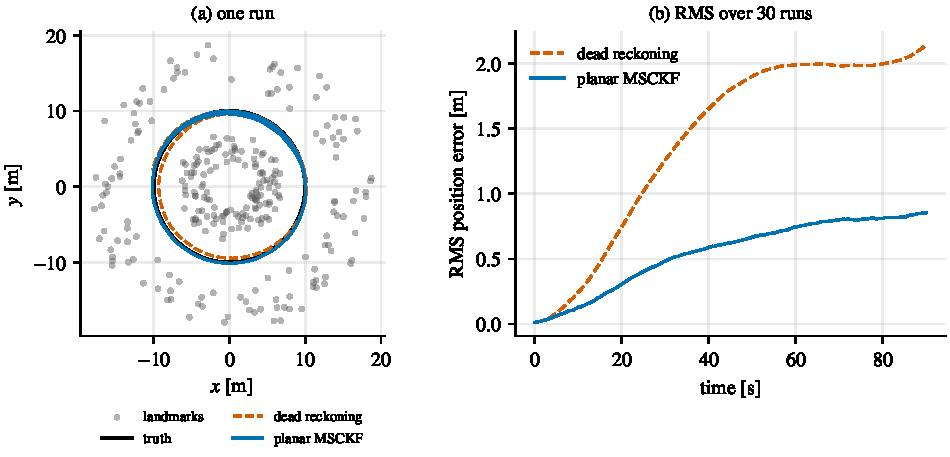
\includegraphics[width=\linewidth]{fig_planar_traj.pdf}
\caption{Planar MSCKF versus dead reckoning. (a) One run. (b) Root-mean-square position error over 30 Monte Carlo runs: after
\SI{90}{s}, \SI{0.85}{m} for the MSCKF against \SI{2.1}{m} for odometry alone.}
\label{fig:planar-traj}
\end{figure}

\begin{figure}[t]
\centering
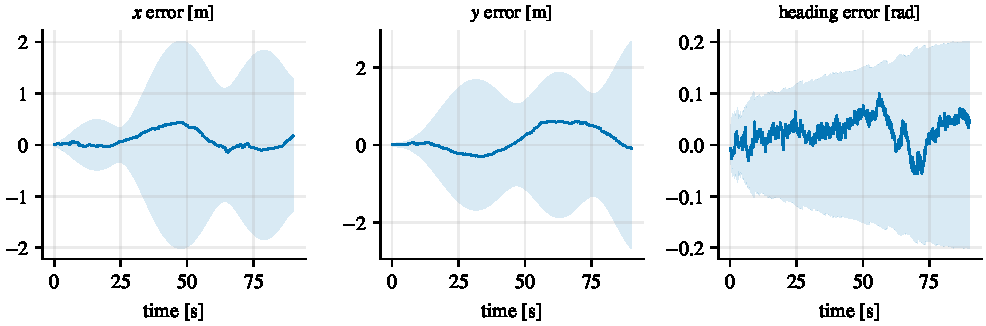
\includegraphics[width=\linewidth]{fig_planar_err.pdf}
\caption{Estimation errors of one run with the filter's $\pm3\sigma$ envelopes (shaded). The position envelopes oscillate because most of the position
uncertainty is perpendicular to the direction of travel, which rotates as the robot circles.}
\label{fig:planar-err}
\end{figure}

\begin{figure}[t]
\centering
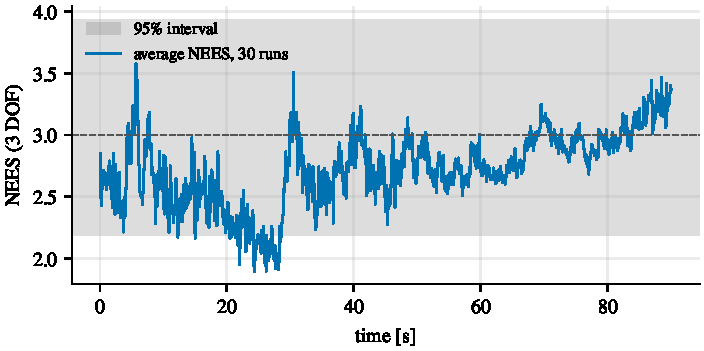
\includegraphics[width=0.8\linewidth]{fig_planar_nees.pdf}
\caption{Average NEES of the robot pose over 30 runs, with the 95\% acceptance interval of \cref{eq:anees-bounds}.}
\label{fig:planar-nees}
\end{figure}

The results (\cref{fig:planar-traj,fig:planar-err,fig:planar-nees}) illustrate four points.
\begin{enumerate}
  \item \textbf{The camera helps, mostly through the heading.} Odometry alone accumulates a heading error with standard deviation
        $\sigma_\omega\sqrt{t} = \SI{0.19}{rad}$ after \SI{90}{s}. The MSCKF ends at about \SI{0.07}{rad}: the camera measures the relative rotation between clones far
        better than the gyro-like turn rate, and because heading errors turn into cross-track position errors, the position error drops by a
        factor of 2.5.
  \item \textbf{The error still grows.} Even with the camera, the heading and position uncertainties grow without bound (\cref{fig:planar-err}).
        This is not a failure: global position and heading are unobservable (\cref{sec:planar-unobservable}), and an odometry filter without loop
        closures can only slow their drift, never stop it. The along-track error is set by the odometry speed noise alone, since a monocular camera
        cannot measure scale (the worked example above).
  \item \textbf{The filter is consistent.} The errors stay inside their $3\sigma$ envelopes, and the average NEES stays inside its acceptance
        interval, apart from mildly conservative dips below it between about 12 and \SI{28}{s}. The gate rejected 5.2\% of the features, close to the 5\% that a $\chi^2_{0.95}$ gate should reject when the filter is
        consistent and every feature is a good one; a much larger rate would signal an overconfident filter or bad data.
  \item \textbf{But the NEES creeps upward.} In the second half of the run its 15-second averages rise steadily, from 2.75 to 2.86 to 3.05, with peaks near 3.5. It is still inside the
        interval, but the trend is systematic: the filter is beginning to believe it knows the heading better than it does. The mechanism, and its cure, are the subject of \cref{ch:observability}.
\end{enumerate}

% ------------------------------------------------------------------------------
\section{The unobservable directions}
\label{sec:planar-unobservable}
\index{unobservable directions!planar}

Suppose we rotate the entire world, the trajectory and every feature, about the origin by a small angle, or translate it. Odometry measures
speed and turn rate in the body frame and does not notice. The camera measures bearings relative to the robot and does not notice either. No
sensor can therefore distinguish the true world from the rotated or translated one: these three directions are \emph{unobservable}
(\cref{sec:observability-linear}), and the filter should never gain information along them.

In error-state coordinates the three directions are the columns of
\begin{equation}
  N = \begin{bmatrix} N_t & N_r \end{bmatrix}, \qquad
  N_t = \begin{bmatrix} I_2 \\ 0 \\ I_2 \\ 0 \\ \vdots \end{bmatrix}, \qquad
  N_r = \begin{bmatrix} \Omega\hat p \\ 1 \\ \Omega\hat p_1 \\ 1 \\ \vdots \end{bmatrix},
  \label{eq:planar-nullspace}
\end{equation}
with one block pair for the robot and one for each clone. $N_t$ shifts every position by the same vector. $N_r$ is the derivative of a rotation
about the origin: a point $p$ moves by $\delta\,\Omega p$, and every heading increases by $\delta$.

\begin{proposition}[The planar nullspace]
\label{prop:planar-nullspace}
If all Jacobians are evaluated at one common set of estimates, then:
\begin{enumerate}
  \item every feature Jacobian satisfies $H_{x,j}N_t + H_{f,j} = 0$ and $H_{x,j}N_r + H_{f,j}\,\Omega\hat p_f = 0$, and therefore the projected Jacobian
        satisfies $H_{o,j}N = 0$;
  \item the exact transition \eqref{eq:planar-phi} maps the nullspace at step $k$ to the nullspace at step $k+1$, $\Phi_kN(\hat x_k) = N(\hat x_{k+1})$;
  \item cloning maps $N$ to the nullspace of the augmented state, $JN = N_{\text{aug}}$.
\end{enumerate}
\end{proposition}
\begin{proof}
(1) Row $i$, translation: $-J_\pi R_i\T + J_\pi R_i\T = 0$. Rotation: using $R_i\T\Omega = \Omega R_i\T$ (\cref{lem:omega}(3)),
\begin{equation*}
  -J_\pi R_i\T\Omega\hat p_i - J_\pi\Omega\hat p_{b,i} + J_\pi R_i\T\Omega\hat p_f = J_\pi\big(\Omega R_i\T(\hat p_f - \hat p_i) - \Omega\hat p_{b,i}\big) = J_\pi(\Omega\hat p_{b,i} - \Omega\hat p_{b,i}) = 0 .
\end{equation*}
Multiplying by $A_j\T$ and using $A_j\T H_{f,j} = 0$ gives $A_j\T H_{x,j}N = 0$.
(2) On the robot block, $\Phi_k(I_2, 0) = (I_2, 0)$, and $\Phi_k(\Omega\hat p_k, 1) = (\Omega\hat p_k + \Omega(\hat p_{k+1} - \hat p_k), 1) = (\Omega\hat p_{k+1}, 1)$; clone blocks are untouched.
(3) The new clone copies the robot's rows of $N$, which are exactly the rows a clone at $\hat p$ should have.
\end{proof}

In words: the linearized filter has the same three unobservable directions as the real system, \emph{as long as every Jacobian uses the same
estimate of each quantity}. A real filter cannot honour this condition. The transition $\Phi_k$ uses $\hat p_{k+1} - \hat p_k$ computed from the
estimate before the update at step $k+1$, while the next transition starts from the corrected estimate; and a clone is linearized at its
current, corrected estimate, not at the value it had when it was created. The identities of \cref{prop:planar-nullspace} then hold only
approximately, the linearized system has an observable heading that the real system does not, and the filter slowly gains spurious heading
information. That is the upward creep in \cref{fig:planar-nees}. \Cref{ch:observability} analyses it in the planar EKF-SLAM setting, where it is most
visible, and shows how First-Estimates Jacobians restore the nullspace.

% ------------------------------------------------------------------------------
\section{From the plane to three dimensions}
\label{sec:planar-to-3d}

\Cref{tab:planar-to-3d} lists every difference between the planar filter and the project's filter. None of them changes the structure of
\cref{alg:planar-msckf}; each changes a formula inside it.

\begin{table}[t]
\centering
\small
\caption{The planar MSCKF and its three-dimensional counterpart.}
\label{tab:planar-to-3d}
\begin{tabularx}{\linewidth}{@{}>{\raggedright\arraybackslash}p{0.2\linewidth}>{\raggedright\arraybackslash}X>{\raggedright\arraybackslash}X@{}}
\toprule
& Plane & Project (AGENTS.md) \\
\midrule
Attitude & heading $\psi$, $R(\psi) = \exp(\psi\Omega)$ & $q_{wb}$, $R_{wb}$, $\Exp$ (\cref{ch:lie}) \\
Error and retraction & $\delta\psi = \psi - \hat\psi$; local and global coincide & local (right) perturbation $q = \hat q\otimes\Exp_q(\delta\theta)$ (C4) \\
Skew operator & $\Omega$, commutes with every $R(\psi)$ & $\sx{\cdot}$; $R\sx{v}R\T = \sx{Rv}$, no commutation \\
Jacobian of $R\T a$ w.r.t.\ the rotation error & $-\Omega R\T a$ & the inverse-action row of \cref{tab:jacobians} \\
Motion sensor & odometry $(v, \omega)$, no biases & IMU $(a_m, \omega_m)$ with gravity and biases (C6) \\
State & $(p, \psi)$ + clones, $3 + 3N$ & $(p, v, q, b_a, b_g)$ + clones, $15 + 6N$ (C3) \\
Camera & 1D bearing $z = y/x$ & 2D normalized $(x/z, y/z)$, through $T_{bc}$ (C6) \\
Constraints per feature & $M - 2$ & $2M - 3$ \\
Reset Jacobian & $1$ & $I - \tfrac12\sx{\delta\hat\theta}$ per attitude (F4) \\
Unobservable directions & 2 translations + heading & 3 translations + yaw (roll and pitch are observable through gravity) \\
\bottomrule
\end{tabularx}
\end{table}

\begin{takeaways}
\begin{itemize}
  \item In the plane every MSCKF Jacobian takes a line: $\partial z/\partial\delta\psi_i = -(1 + z^2)$, $\partial z/\partial\delta p_i = -J_\pi R_i\T$, $H_f = J_\pi R_i\T$.
  \item A camera measures rotation independently of depth, and translation only through parallax ($1/x$).
  \item A feature seen $M$ times gives $M - 2$ constraints in the plane ($2M - 3$ in space); for three views the constraint is a second difference
        that measures the ratio of baselines and the relative headings, but not scale, global position or global heading.
  \item The planar filter is consistent and reduces the dead-reckoning error by a factor of about 2.5, yet its NEES creeps upward: the first sign
        of the spurious heading information studied in \cref{ch:observability}.
  \item The step to three dimensions changes formulas, not structure: non-commuting rotations, the local perturbation, gravity, biases and the reset Jacobian.
\end{itemize}
\end{takeaways}

\begin{exercises}
  \item Verify \cref{prop:planar-H} by finite differences at a random clone pose and feature. Then explain $\partial z/\partial\delta\psi = -(1 + z^2)$ using
        only the bearing angle $\beta = \arctan z$.
  \item Show that $I + F_c\Dt$ and the exact $\Phi_k$ of \eqref{eq:planar-phi} differ by $O(\Dt^2)$, and identify the term.
  \item Add a turn-rate bias $b_\omega$ ($\omega_m = \omega + b_\omega + n_\omega$, $\dot b_\omega = n_b$) to the planar state. Derive the new column of $F_c$ and the new
        row of $G_c$, and show that the bias is observable once the camera sees features. Compare with the gyroscope-bias block of the
        three-dimensional filter.
  \item Repeat the worked example with unequal baselines, $\hat p_3 = (0, 2)$. Find $a$, and show that the projected residual measures the
        ratio of the two baselines.
  \item In the worked example, show that moving the \emph{middle} clone along the viewing direction $x_w$ is invisible to $H_o$, while moving the
        \emph{first} clone along $x_w$ is visible. Interpret the difference in terms of the bearing each clone has to the feature.
  \item Why does a 1D camera need three views of a feature to say anything about the poses, while a 2D camera needs only two? Relate the answer
        to the dimensions of $H_f$.
  \item Run \code{scripts/planar\_sims.py} with window sizes $N_{\max} = 3, 5, 10, 20$ and plot the final RMS position error. Explain the trend, and what
        limits the benefit of a longer window.
  \item Prove part (1) of \cref{prop:planar-nullspace} without using the closed-form Jacobians: argue directly that a measurement function that depends only
        on $R(\psi_i)\T(p_f - p_i)$ cannot change under a common rotation or translation of all positions.
  \item Replace the bearing camera by a range-and-bearing sensor. How many constraints does a feature seen $M$ times give? Which of the unobservable
        directions of \eqref{eq:planar-nullspace} become observable, if any?
\end{exercises}
\input{chapters/solutions/27_planar_msckf}

\chapter{The Complete Algorithm}
\label{ch:fullalgo}

\begin{objectives}
\begin{itemize}
  \item Assemble every component into one event-driven estimator, with the correct order of operations.
  \item Estimate the computational budget and map the algorithm onto the project's software architecture.
  \item Diagnose the most common failures from their symptoms.
\end{itemize}
\end{objectives}

% ------------------------------------------------------------------------------
\section{The event loop}

The estimator consumes a single, time-ordered stream of sensor events. Milestone 3 builds it by merging the presorted IMU,
image (and, for testing, pose) arrays with a two-pointer merge, with the rule that an IMU sample precedes any other event
with the same timestamp. \Cref{alg:msckf} shows the loop.

\begin{algorithm}[t]
\caption{Monocular MSCKF}
\label{alg:msckf}
\begin{algorithmic}[1]
\Require event stream, calibration, noise parameters
\LineComment{load phase: allocation allowed}
\State parse data and calibration; build the event arrays; construct the filter and front end with fixed-max workspaces
\State initialize $(\hat x, P)$ (ground truth in the project, logged; static initialization otherwise)
\LineComment{streaming phase: no allocation in the core}
\For{each event $e$ in timestamp order}
  \If{$e$ is an IMU sample at $t$}
    \State propagate nominal state and covariance from $t_{prev}$ to $t$ \Comment{\cref{ch:strapdown,ch:errordyn}}
  \ElsIf{$e$ is an image at $t_c$}
    \State propagate to $t_c$ (interpolated IMU) \Comment{exact image time}
    \State front end: track, verify, undistort; update track histories \Comment{\cref{ch:frontend}}
    \State process tracks that were lost in this image \Comment{\cref{alg:msckf-update}}
    \If{$N = $ \code{kMaxClones}}
      \State process tracks with an observation at the oldest clone
      \State marginalize the oldest clone in place \Comment{\cref{ch:cloning}}
    \EndIf
    \State clone $(\hat p, \hat q)$; $P \gets JPJ\T$; attach this image's observations to the new clone
  \EndIf
  \State log state, $\diag(P)$, NIS and gate statistics to the preallocated buffer
\EndFor
\end{algorithmic}
\end{algorithm}

Three ordering rules are essential.
\begin{enumerate}
  \item \textbf{Propagate before you update.} A measurement at time $t$ must be applied to the state at time $t$, never to the
        state at the previous IMU sample.
  \item \textbf{Use a clone's observations before you delete it.} Every feature with an observation at the oldest clone is
        processed before that clone is marginalized; otherwise its information is lost.
  \item \textbf{Use each observation once.} After a track has been used, its observations are discarded. If the feature keeps
        being tracked, later observations form a new track.
\end{enumerate}
With the order of \cref{alg:msckf}, the window never holds more than \code{kMaxClones} clones, which keeps the covariance within its
fixed maximum size. A feature processed because its oldest clone is leaving cannot use the current image's observation in that
update, because the new clone does not exist yet. Implementations that clone first need room for one extra clone. Either
choice is valid; the storage bound must match it.
The planar filter of \cref{ch:planar} runs exactly this loop (\cref{alg:planar-msckf}) in a few lines of Python, which makes it a
convenient place to experiment with the ordering rules before committing to them in C++.

\begin{figure}[t]
\centering
\begin{tikzpicture}[xscale=0.9, yscale=1.0]
  \draw[->, thick] (0,0) -- (15.5,0) node[right, font=\footnotesize] {$t$};
  \foreach \x in {0,0.25,...,15.0} \draw[black!45] (\x,-0.08) -- (\x,0.08);
  \node[font=\scriptsize, black!60, below] at (0.6,-0.15) {IMU, 200 Hz};
  \foreach \k/\x in {1/1.25, 2/3.75, 3/6.25, 4/8.75, 5/11.25, 6/13.75} {
    \draw[primary, thick] (\x,-0.25) -- (\x,0.6);
    \draw[fill=primarylight, draw=primary] (\x-0.25,0.6) rectangle (\x+0.25,1.0);
    \node[font=\scriptsize] at (\x,0.8) {$C_\k$};
  }
  \node[font=\scriptsize, primary, below] at (3.75,-0.25) {image (20 Hz)};
  % features
  \draw[plotgreen, very thick] (1.25,1.35) -- (8.75,1.35) node[right, font=\scriptsize] {track $f_1$ lost $\Rightarrow$ update};
  \fill[plotgreen] (1.25,1.35) circle (2pt) (3.75,1.35) circle (2pt) (6.25,1.35) circle (2pt) (8.75,1.35) circle (2pt);
  \draw[plotorange, very thick] (3.75,1.85) -- (13.75,1.85);
  \fill[plotorange] (3.75,1.85) circle (2pt) (6.25,1.85) circle (2pt) (8.75,1.85) circle (2pt) (11.25,1.85) circle (2pt) (13.75,1.85) circle (2pt);
  \node[font=\scriptsize, plotorange, align=left, right] at (13.85,1.95) {$f_2$: oldest clone\\leaving $\Rightarrow$ update};
  \draw[decorate, decoration={brace, amplitude=4pt}] (3.5,2.25) -- (14.0,2.25) node[midway, above=5pt, font=\scriptsize] {window (example \code{kMaxClones} = 5)};
  \draw[conv, ->] (1.25,2.5) -- (1.25,1.1) node[pos=0, above, font=\scriptsize, align=center] {$C_1$ marginalized\\when $C_6$ arrives};
\end{tikzpicture}
\caption{Timeline of the MSCKF. The IMU propagates at 200~Hz; each image creates a clone; feature tracks are processed when
they end or when the clone holding their oldest observation is about to leave the window.}
\label{fig:timeline}
\end{figure}

% ------------------------------------------------------------------------------
\section{Initialization and the first seconds}

The project initializes from ground truth, which removes the hardest failure mode from early testing and is logged as a use of
ground truth (Milestone 10b). With static initialization (\cref{ch:strapdown}), the first seconds are delicate: the yaw is
arbitrary, the accelerometer bias is entangled with tilt, and the window contains few clones with little parallax. Generous
initial covariances, and a check that enough features with sufficient parallax exist before trusting visual updates, avoid
early divergence. Inspect the IMU data of each EuRoC sequence before running on it: a static start followed by vigorous
motion is the easiest case for initialization, and a fast start the hardest.

% ------------------------------------------------------------------------------
\section{Computational budget}

With $N = 10$ clones the error state has $n = 75$ dimensions. Rough flop counts per operation:
\begin{center}\small
\begin{tabular}{@{}l l r@{}}
\toprule
Operation & Frequency & Cost (flops) \\
\midrule
Nominal propagation & 200 Hz & $\sim10^2$ \\
$P_{II}$, $P_{IC}$ propagation & 200 Hz & $\sim4\times10^4$ \\
Cloning ($P \gets JPJ\T$ as block copies) & 20 Hz & $\sim10^4$ \\
Per feature: triangulation, projection, gating ($M = 6$) & per track & $\sim10^5$ \\
QR compression of $d = 450$ rows & per update & $\sim5\times10^6$ \\
Update ($S$, gain, Joseph) with $n = 75$ & per update & $\sim6\times10^6$ \\
Front end (KLT on 150 features) & 20 Hz & dominant in time \\
\bottomrule
\end{tabular}
\end{center}
The filter core needs on the order of $10^7$ flops per image, a few milliseconds on an embedded processor and well under a
millisecond on a desktop. The front end is usually the bottleneck in wall-clock time. The cubic growth with $n$ is why the window
is short and why QR compression matters for large stacks.

% ------------------------------------------------------------------------------
\section{Software architecture}

\begin{figure}[t]
\centering
\begin{tikzpicture}[node distance=8mm and 10mm]
  \node[block, minimum width=48mm, align=left] (core) {\textbf{vio\_core} (static, Eigen only)\\ \footnotesize so3, imu\_integrator, es\_ekf,\\ \footnotesize camera\_model, triangulation, msckf\_update};
  \node[block, minimum width=34mm, above left=10mm and -14mm of core, align=left] (io) {\textbf{vio\_io}\\ \footnotesize dataset\_loader, telemetry\\ \footnotesize + YAML parser};
  \node[block, minimum width=34mm, above right=10mm and -14mm of core, align=left] (fe) {\textbf{vio\_frontend}\\ \footnotesize visual\_frontend\\ \footnotesize + OpenCV};
  \node[block, minimum width=30mm, above=24mm of core, fill=white] (app) {\textbf{vio\_app}\\ \footnotesize main.cpp};
  \draw[->, thick] (io) -- (core); \draw[->, thick] (fe) -- (core);
  \draw[->, thick] (app) -- (io); \draw[->, thick] (app) -- (fe); \draw[->, thick] (app) -- (core);
  \node[font=\footnotesize, align=center, below=2mm of core] {arrows: ``depends on''. OpenCV never reaches \code{vio\_core};\\ each test links only the library it tests.};
\end{tikzpicture}
\caption{Library targets of the project (AGENTS.md). Dependencies point one way, so the estimator core can be built, tested and
reasoned about without the I/O and vision libraries.}
\label{fig:architecture}
\end{figure}

\Cref{fig:architecture} shows how the algorithm maps to the project's targets. The zero-allocation discipline applies to
\code{vio\_core}, which contains everything executed per IMU sample and per update. The front end may allocate but must reuse its
buffers, and the I/O layer allocates freely during loading.

% ------------------------------------------------------------------------------
\section{Debugging guide}

\begin{table}[t]
\centering\small
\begin{tabularx}{\textwidth}{@{}>{\raggedright\arraybackslash}p{4.4cm} X@{}}
\toprule
\textbf{Symptom} & \textbf{Likely causes} \\
\midrule
Altitude diverges at about $2g$ in IMU-only propagation & gravity or specific-force sign; $g_w$ added twice \\
Position diverges within seconds even with ground-truth init & $R_{wb}$ used as $R_{bw}$; quaternion $w/z$ swapped at load; gyro and accel columns or biases swapped; degrees vs radians \\
Rotation matrices slowly scale vectors & missing quaternion normalization \\
NaN after a while & missing Taylor branch; $\Log$ near $\pi$; $\Jrinv$ evaluated beyond $\pi$; feature at zero depth; Cholesky of a non-PD $S$ \\
Corrections systematically make things worse & sign of $H$ or of the residual; injection on the wrong side of the quaternion; global vs local convention mixed \\
Covariance loses symmetry or positive definiteness & simple update form instead of Joseph; missing symmetrization; aliasing in Eigen block products \\
Nearly all features fail the gate & overconfident $P$; $T_{bc}$ inverted; pixel noise used in normalized units (or vice versa); distortion not removed; timestamps misaligned \\
Gate rejects nothing & $R_z$ or $\sigma_{uv}$ far too large; gate threshold indexed with the wrong dimension \\
Slowly growing yaw error with healthy NIS & expected EKF inconsistency along unobservable yaw (\cref{ch:observability}) \\
Scale drift & little acceleration (degenerate motion); accelerometer noise or bias badly tuned \\
Works on synthetic data, fails on EuRoC & extrinsics, time offset, distortion, noise inflation, initialization, IMU gaps \\
Results differ between runs & uninitialized memory (run the sanitizers); unseeded random generators \\
\bottomrule
\end{tabularx}
\caption{Symptoms and their most frequent causes.}
\label{tab:debugging}
\end{table}

\Cref{tab:debugging} collects the failures that experience shows are most common. The milestone structure of the project is itself
the most effective debugging tool: each layer is verified against known truth before the next is built on top of it, so a new
failure is almost always in the newest layer.

\section{What to expect on EuRoC}

Published monocular filter-based estimators reach absolute trajectory errors of the order of 0.1 to 0.5~m on the machine-hall
sequences, depending on features, tuning and initialization, with the difficult sequences (fast motion, motion blur, dark
regions) considerably worse~\cite{delmerico2018benchmark}. Milestone 10b sets a first-pass target of 0.5~m on MH\_01 and a stretch target of
0.2~m. Yaw and position drift without bound; roll and pitch remain accurate throughout; velocity and biases converge within the
first seconds of excitation.

\begin{takeaways}
\begin{itemize}
  \item One time-ordered stream; propagate to each event's time before applying it.
  \item At each image: process lost tracks; if the window is full, process the oldest clone's tracks and marginalize it; then clone.
  \item The core costs about $10^7$ flops per image; the front end usually dominates the run time.
  \item Dependencies point one way: \code{vio\_core} knows nothing about files, YAML or OpenCV.
  \item Most failures map to a small set of sign, frame, unit and timing errors; test each layer against truth.
\end{itemize}
\end{takeaways}

\begin{exercises}
  \item Write the event-loop pseudocode for the alternative ordering (clone first, then process and marginalize). What capacity
        does it require, and what does it gain?
  \item Instrument a run to record the number of features processed per update, their observation counts, and the stacked row
        count $d$. Choose the compile-time row cap from the distribution.
  \item For each row of \cref{tab:debugging}, design a unit or integration test that would have caught the cause before the full
        system was assembled.
\end{exercises}
\input{chapters/solutions/28_full_algorithm}


\part{Beyond the Baseline}
\chapter{Observability and Consistency of VIO}
\label{ch:observability}
\chaptermark{Observability and Consistency} % short running header

\begin{objectives}
\begin{itemize}
  \item Define observability for nonlinear systems, and test it with Lie derivatives.
  \item Prove that VIO has four unobservable directions and write them in the project's error coordinates.
  \item Show, in the planar EKF-SLAM problem where every step can be computed, exactly how the standard EKF acquires spurious information,
        and see it happen in a Monte Carlo simulation.
  \item Prove that First-Estimates Jacobians restore the correct unobservable subspace, and understand the alternatives: the
        observability-constrained EKF, the invariant EKF and robocentric formulations.
  \item Know the degenerate motions that remove further information.
\end{itemize}
\end{objectives}

The planar MSCKF of \cref{ch:planar} was consistent, but its NEES crept upward. This chapter explains the creep. The explanation needs one
new idea, observability, and one careful computation, the observability matrix of a linearized filter. The computation is done in full for
planar EKF-SLAM, the setting in which the effect was first understood~\cite{julier2001counter, bailey2006consistency, huang2010observability},
and then carried over to VIO.

% ------------------------------------------------------------------------------
\section{Observability}

\subsection{Indistinguishable states}

Consider a system $\dot x = f(x, u)$ with output $y = h(x)$. Two initial states $x_0$ and $x_0'$ are \term{indistinguishable} if, for every input
signal $u(\cdot)$, they produce the same output signal $y(\cdot)$. No estimator, however clever, can tell them apart: the data are identical. A
system is \emph{observable} at $x_0$ if no other state is indistinguishable from it. Since estimators work locally, the useful notion is
local: $x_0$ is \termi{locally weakly observable}{observability!local weak} if it can be distinguished, over arbitrarily short time intervals, from
every state in some neighborhood of it.

For linear systems the question is settled by the observability matrix (\cref{thm:obs-rank}). For a time-varying linear system
$\delta x_{k+1} = \Phi_k\delta x_k$, $r_k = H_k\delta x_k$ the same object reads as follows.

\begin{definition}[Observability matrix]
\label{def:obs-matrix}
The observability matrix over steps $1, \dots, k$ is
\begin{equation}
  \mathcal{O} = \begin{bmatrix} H_1 \\ H_2\Phi_1 \\ H_3\Phi_2\Phi_1 \\ \vdots \\ H_k\Phi_{k-1}\cdots\Phi_1 \end{bmatrix}.
\end{equation}
An initial error $\delta x_1 \in \nullsp(\mathcal{O})$ produces no change in any measurement, so it cannot be detected.
$\nullsp(\mathcal{O})$ is the \term{unobservable subspace}.
\end{definition}

A Kalman filter can gain information only in directions outside $\nullsp(\mathcal{O})$. Along unobservable directions its covariance may grow
(from process noise) but must never shrink. This is the property that the standard EKF violates.

\subsection{Nonlinear observability and Lie derivatives}

For a nonlinear system the observability matrix is replaced by derivatives of the output along the dynamics. Suppose the dynamics are
\emph{control-affine}, $\dot x = f_0(x) + \sum_i f_i(x)\,u_i$, as kinematic models usually are (the inputs are the measured rates and
accelerations). The \termi{Lie derivative}{Lie derivative} of a scalar function $\varphi$ along a vector field $f$ is its rate of change along the flow of $f$,
\begin{equation}
  L_f\varphi(x) = \nabla\varphi(x)\cdot f(x),
\end{equation}
and repeated derivatives are written $L_gL_f\varphi = \nabla(L_f\varphi)\cdot g$. Differentiating the output along a trajectory gives
\begin{equation}
  y = h(x), \qquad \dot y = L_{f_0}h + \sum_i u_i\,L_{f_i}h, \qquad \ddot y = \dots
\end{equation}
Because the inputs can be varied freely, each Lie derivative $L_{f_i}h$ is, in effect, a separate measured function of the state, and so are
the higher ones. If enough of them are available, their values pin down the state.

\begin{theorem}[Observability rank condition~\cite{hermann1977nonlinear}]
\label{thm:obs-rank-nonlinear}
Let $d\mathcal{O}(x)$ be the span of the gradients of $h$ and of all its repeated Lie derivatives $L_{f_{i_1}}\cdots L_{f_{i_m}}h$ along the vector fields of
the system. If $\dim d\mathcal{O}(x_0) = n$, the system is locally weakly observable at $x_0$.
\end{theorem}
\begin{proof}[Idea of the proof]
Choose $n$ of the functions whose gradients are independent at $x_0$ and stack them into $\Psi(x) \in \R^n$. Each is determined by the output
and the inputs (by differentiation), and $\Psi$ has an invertible Jacobian at $x_0$, so by the inverse function theorem it is one-to-one near $x_0$.
Two nearby states with the same outputs would have the same $\Psi$, hence coincide.
\end{proof}

For a linear system, $f_0 = Ax$ and $h = Cx$, the gradients are $C, CA, CA^2, \dots$: the rank condition is \cref{thm:obs-rank}. For analytic systems the
condition is also necessary in a generic sense, so a rank deficiency at typical states signals a genuine family of indistinguishable states.

\begin{worked}[a planar robot and a landmark]
A planar robot (\cref{ch:planar}) with pose $(p, \psi)$ measures the position of a landmark $\ell$ in its body frame, $h = R(\psi)\T(\ell - p) \in \R^2$. Its kinematics
are $\dot p = R(\psi)e_1\,v$ and $\dot\psi = \omega$, that is $f_v = (R(\psi)e_1, 0)$ and $f_\omega = (0, 1)$ with inputs $v$ and $\omega$.

\emph{Unknown landmark.} The state is $x = (p, \psi, \ell) \in \R^5$. With $\partial(R\T a)/\partial\psi = -\Omega R\T a$ (\cref{lem:omega}),
\begin{equation*}
  \nabla h = \begin{bmatrix} -R\T & -\Omega h & R\T \end{bmatrix}, \qquad
  L_{f_v}h = -R\T Re_1 = -e_1, \qquad L_{f_\omega}h = -\Omega h .
\end{equation*}
The first Lie derivative is constant (its gradient is zero), and $\nabla(L_{f_\omega}h) = -\Omega\nabla h$ has the same row space as $\nabla h$. Every further
derivative repeats the pattern, so $\dim d\mathcal{O} = 2$: three of the five directions are unobservable. They are the two global translations and the
global rotation, exactly the directions of \cref{sec:planar-unobservable}.

\emph{Known landmark.} If $\ell$ is known, $x = (p, \psi) \in \R^3$, the gradients are $[-R\T\ \ {-\Omega h}]$ and its multiples by $\Omega$, and the rank is 2: one
direction is unobservable. It is the rotation of the robot about the landmark, which leaves the body-frame landmark position unchanged. One known
landmark fixes position but not heading; two fix both.
\end{worked}

% ------------------------------------------------------------------------------
\section{The four unobservable directions of VIO}
\index{unobservable directions!VIO}

\begin{theorem}[Unobservable directions of VIO]
\label{thm:vio-unobservable}
For monocular VIO with point features, applying the same global translation $t$ and the same rotation $R_z(\alpha)$ about the
gravity direction to all positions, velocities, attitudes, clones and features leaves every IMU and camera measurement
unchanged. The state is therefore unobservable along these four directions.
\end{theorem}
\begin{proof}
Under $p \mapsto R_zp + t$, $v \mapsto R_zv$, $R_{wb} \mapsto R_zR_{wb}$, $p_f \mapsto R_zp_f + t$, with biases unchanged:
\begin{itemize}
  \item the gyroscope measures $\sx{\omega_b} = R_{wb}\T\dot R_{wb}$, which is invariant because $R_z$ is constant;
  \item the accelerometer measures $R_{wb}\T R_z\T(R_za_w - g_w) = R_{wb}\T(a_w - R_z\T g_w) = R_{wb}\T(a_w - g_w)$, because a rotation about
        gravity leaves $g_w$ unchanged;
  \item the camera sees $R_{bc}\T\big(R_{wb}\T R_z\T(R_zp_f + t - R_zp - t) - p_{bc}\big) = R_{bc}\T\big(R_{wb}\T(p_f - p) - p_{bc}\big)$.
\end{itemize}
All measurements are identical, so the transformed and original trajectories cannot be distinguished.
\end{proof}

Rotations about horizontal axes are \emph{not} in this family, because they would rotate gravity in the accelerometer equation;
roll and pitch are observable. Scaling is not either, because it would scale the accelerations the accelerometer measures;
scale is observable as long as the vehicle accelerates. That the remaining directions (velocity, roll, pitch, scale, biases) \emph{are}
observable under general motion is proved with the rank condition of \cref{thm:obs-rank-nonlinear}; see~\cite{hesch2014consistency} for the
computation.

Linearizing the transformation gives the unobservable directions in the project's error coordinates. With $e_z$ the vertical
unit vector, a small yaw rotation $\alpha$ and a small translation $t$ change the state by (verified numerically):
\begin{equation}
  \underbrace{\begin{bmatrix} \delta p \\ \delta v \\ \delta\theta \\ \delta b_a \\ \delta b_g \\ \delta p_i \\ \delta\theta_i \\ \delta p_f \end{bmatrix}}_{\text{error state}}
  = \underbrace{\begin{bmatrix}
    I_3 & -\sx{\hat p}\,e_z \\
    0 & -\sx{\hat v}\,e_z \\
    0 & \hat R\T e_z \\
    0 & 0 \\
    0 & 0 \\
    I_3 & -\sx{\hat p_i}\,e_z \\
    0 & \hat R_i\T e_z \\
    I_3 & -\sx{\hat p_f}\,e_z
  \end{bmatrix}}_{N}
  \begin{bmatrix} t \\ \alpha \end{bmatrix}.
  \label{eq:nullspace-N}
\end{equation}
The last row applies only to formulations that keep features in the state. The position entries follow from
$R_z(\alpha)p \approx p + \alpha\,e_z\times p = p - \alpha\sx{p}e_z$; the attitude entry is $\hat R\T e_z$ because the error is
local: $\Exp(\alpha e_z)\hat R = \hat R\,\Exp(\alpha\hat R\T e_z)$, a rotation about the world vertical expressed in body axes. Every column of $N$ \emph{depends on
the estimate}: the yaw column involves $\hat p$, $\hat v$, $\hat R$ and the clone and feature estimates. That dependence is the root of the problem.
\Cref{eq:planar-nullspace} is the planar version, with $\Omega\hat p$ in place of $-\sx{\hat p}e_z$.

% ------------------------------------------------------------------------------
\section{Why the standard EKF becomes overconfident}

If every Jacobian were evaluated at the true state, the linearized system would satisfy $\mathcal{O}N = 0$ at all times, and the
filter would never gain information along $N$. The EKF instead evaluates each Jacobian at the best estimate available when it is
computed. The transition matrix $\Phi_k$ is evaluated at the estimate after the update at step $k$, while the measurement Jacobian at step $k$ was evaluated
at the estimate before that update. The same physical state enters the observability matrix linearized at two different points, and the products
$H_k\Phi_{k-1}\cdots\Phi_1N$ no longer cancel. The planar EKF-SLAM problem shows this in a computation short enough to do completely.

\subsection{Planar EKF-SLAM}
\index{EKF-SLAM!inconsistency}\index{inconsistency!EKF}

The state is the robot pose and $L$ landmarks, $x = (p, \psi, \ell_1, \dots, \ell_L)$, with additive errors. Odometry propagates the robot
($p_{k+1} = p_k + R(\psi_k)e_1v_m\Dt$, $\psi_{k+1} = \psi_k + \omega_m\Dt$), landmarks are static, and an observation of landmark $j$ is its position in the
body frame, $z = R(\psi)\T(\ell_j - p) + n$. Writing $\hat x_{k|k-1}$ for the propagated estimate at step $k$ and $\hat x_{k|k}$ for the updated one, the EKF uses
\begin{align}
  \Phi_k &= \begin{bmatrix} I_2 & \Omega\,(\hat p_{k+1|k} - \hat p_{k|k}) \\ 0 & 1 \end{bmatrix} \oplus I_{2L}, \label{eq:slam-phi} \\
  H_k &= \begin{bmatrix} -\hat R_k\T & -\Omega\hat R_k\T(\hat\ell_j - \hat p_{k|k-1}) & 0 \cdots 0 & \hat R_k\T & 0 \cdots 0 \end{bmatrix},
  \qquad \hat R_k = R(\hat\psi_{k|k-1}), \label{eq:slam-H}
\end{align}
where $\Phi_k$ follows from \cref{prop:planar-phi} (the step starts from the updated estimate), $H_k$ from the derivation of \cref{prop:planar-H} without the
projection, and $\hat\ell_j$ is the landmark estimate at the time of the update. The candidate unobservable directions, by the argument of
\cref{sec:planar-unobservable}, are the translations $N_t = (I_2, 0, I_2, \dots, I_2)$ and the rotation
\begin{equation}
  N_r(\bar p, \bar\ell) = \big(\Omega\bar p,\ 1,\ \Omega\bar\ell_1,\ \dots,\ \Omega\bar\ell_L\big),
\end{equation}
built from some reference values $\bar p$, $\bar\ell_j$ of the positions.

\begin{theorem}[Observability of linearized planar EKF-SLAM]
\label{thm:slam-obs}
Let $\Delta_i = \hat p_{i|i} - \hat p_{i|i-1}$ be the correction of the robot position by the update at step $i$, and $D_k = \sum_{i=1}^{k-1}\Delta_i$ (with $D_1 = 0$).
For every $k$, $H_k\Phi_{k-1}\cdots\Phi_1N_t = 0$, while
\begin{equation}
  H_k\Phi_{k-1}\cdots\Phi_1\,N_r(\hat p_{1|0}, \bar\ell) = \hat R_k\T\,\Omega\,\big(D_k + \bar\ell_j - \hat\ell_j\big).
  \label{eq:slam-leak}
\end{equation}
\end{theorem}
\begin{proof}
Each $\Phi_i$ is the identity plus a term in the heading column, so the product is
$\Phi_{k-1}\cdots\Phi_1 = \begin{bmatrix} I & \Omega\,s_k \\ 0 & 1\end{bmatrix} \oplus I$ with
\begin{equation*}
  s_k = \sum_{i=1}^{k-1}\big(\hat p_{i+1|i} - \hat p_{i|i}\big)
      = \sum_{i=1}^{k-1}\big(\hat p_{i+1|i} - \hat p_{i|i-1}\big) - \sum_{i=1}^{k-1}\big(\hat p_{i|i} - \hat p_{i|i-1}\big)
      = \hat p_{k|k-1} - \hat p_{1|0} - D_k ,
\end{equation*}
since the first sum telescopes. Translations: the product leaves $N_t$ unchanged and $H_kN_t = -\hat R_k\T + \hat R_k\T = 0$. Rotation: the product
maps the robot entries $(\Omega\hat p_{1|0}, 1)$ to $(\Omega\hat p_{1|0} + \Omega s_k, 1) = (\Omega(\hat p_{k|k-1} - D_k), 1)$ and leaves the landmark entries alone, so
\begin{equation*}
  H_k(\cdot) = -\hat R_k\T\Omega(\hat p_{k|k-1} - D_k) - \Omega\hat R_k\T(\hat\ell_j - \hat p_{k|k-1}) + \hat R_k\T\Omega\bar\ell_j
  = \hat R_k\T\Omega\big(D_k + \bar\ell_j - \hat\ell_j\big),
\end{equation*}
using $\hat R_k\T\Omega = \Omega\hat R_k\T$; the $\hat p_{k|k-1}$ terms cancel.
\end{proof}

\Cref{eq:slam-leak} is the whole story. The rotation direction stays in the nullspace only if two things vanish:
\begin{itemize}
  \item $D_k$, the accumulated corrections of the robot position. They vanish only if the transition matrices telescope, which requires each $\Phi_i$
        to start where the previous one ended. The EKF starts each $\Phi_i$ from the \emph{updated} estimate $\hat p_{i|i}$, while the previous one ended at the
        \emph{propagated} estimate $\hat p_{i|i-1}$.
  \item $\bar\ell_j - \hat\ell_j$, the change of the landmark estimate between its linearization points. A single fixed reference $\bar\ell_j$ cannot match an
        estimate that every update moves.
\end{itemize}
For generic estimates no other choice of reference values makes \eqref{eq:slam-leak} vanish for all $k$, and the unobservable subspace of the EKF's
linearized model shrinks from three dimensions to two~\cite{huang2010observability}: the heading has become observable. The filter then extracts
\emph{spurious information} about the global heading from measurements that contain none. The size of the leak is set by the size of the
corrections and of the landmark estimate changes; it is largest at loop closures, when a robot that has drifted re-observes old landmarks
and receives large corrections.

\subsection{From planar SLAM to VIO}

The same mechanism operates in VIO. The translation columns of \eqref{eq:nullspace-N} survive, because all Jacobians depend only on
\emph{differences} of positions. The yaw column does not: with estimate-dependent Jacobians $\mathcal{O}N_{\text{yaw}} \neq 0$, and the unobservable
subspace of the EKF's linearized model has dimension three instead of four~\cite{li2013msckf2, hesch2014consistency}. In the MSCKF, the
clones play the role of the landmarks: a clone is created from the propagated estimate, and every later update moves it, so its linearization
point in a measurement Jacobian differs from the one at which it entered the filter. The filter becomes overconfident in yaw, and because
yaw errors couple into position through the trajectory, its position covariance becomes too small as well. On long trajectories the NEES of
yaw and position grows steadily while the NIS can look perfectly healthy: the inconsistency lives in directions the measurements do not see
(\cref{tab:consistency-diagnosis}).

\begin{keyidea}[an inconsistency that no unit test catches]
EKF yaw inconsistency is not a bug in the usual sense: every Jacobian can pass its finite-difference test. It is a property of
linearizing at estimates that change over time. Milestone 10b therefore expects it, and asks for it to be measured and documented
rather than fixed.
\end{keyidea}

% ------------------------------------------------------------------------------
\section{First-Estimates Jacobians}
\label{sec:fej}
\index{First-Estimates Jacobians}\index{FEJ|see{First-Estimates Jacobians}}

The cure suggested by \eqref{eq:slam-leak} is to make both terms vanish by construction: evaluate every Jacobian that involves a state at the
\emph{first} estimate of that state, the value it had when it entered the filter, rather than at the latest one~\cite{huang2008fej, huang2010observability}.

\begin{proposition}[FEJ restores the nullspace]
\label{prop:fej}
In planar EKF-SLAM, evaluate the transition matrix with the propagated estimates at both ends,
\begin{equation}
  \Phi_k^{\mathrm{FEJ}} = \begin{bmatrix} I_2 & \Omega\,(\hat p_{k+1|k} - \hat p_{k|k-1}) \\ 0 & 1 \end{bmatrix} \oplus I,
\end{equation}
and the measurement Jacobian at the propagated robot estimate $\hat x_{k|k-1}$ and at the \emph{first estimate} $\hat\ell_j^{(1)}$ of each landmark. Initialize
each landmark from the propagated robot estimate, $\hat\ell_j^{(1)} = \hat p_{k|k-1} + R(\hat\psi_{k|k-1})z$, with the augmentation Jacobian evaluated there.
Then $\mathcal{O}N = 0$ for all $k$, with $N = [N_t\ \ N_r(\hat p_{1|0}, \hat\ell^{(1)})]$.
\end{proposition}
\begin{proof}
The transition matrices now telescope: $\sum_i(\hat p_{i+1|i} - \hat p_{i|i-1}) = \hat p_{k|k-1} - \hat p_{1|0}$, so $D_k$ is replaced by zero. The landmark linearization
point is fixed at $\hat\ell_j^{(1)}$, which is also the reference value in $N_r$, so $\bar\ell_j - \hat\ell_j = 0$. Both terms of \eqref{eq:slam-leak} vanish.
For a landmark initialized at step $k$, the augmentation Jacobian $[I_2\ \ \Omega R(\hat\psi_{k|k-1})z\ \ 0]$ maps the robot part of $N_r$, $(\Omega\hat p_{k|k-1}, 1)$, to
$\Omega(\hat p_{k|k-1} + R(\hat\psi_{k|k-1})z) = \Omega\hat\ell_j^{(1)}$: exactly the entry $N_r$ needs for the new landmark.
\end{proof}

Only the \emph{Jacobians} change. The residuals are still computed with the latest estimates, the mean is still propagated and updated as
before, and the filter still uses all its information. The price is that each Jacobian is evaluated slightly away from the best estimate,
which adds linearization error; when the first estimates are poor this can matter, but in practice FEJ filters are markedly more consistent and
usually more accurate.

\begin{figure}[t]
\centering
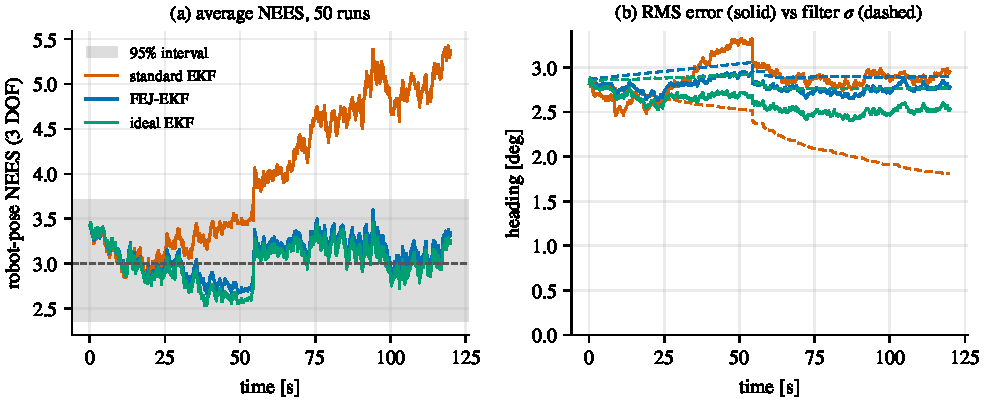
\includegraphics[width=\linewidth]{fig_fej.pdf}
\caption{Planar EKF-SLAM, 50 Monte Carlo runs. (a) Average NEES of the robot pose: the standard EKF leaves the 95\% interval after the first loop
closure (about \SI{55}{s}) and keeps rising, while the FEJ-EKF and the ideal EKF stay consistent. (b) Heading: actual RMS error (solid) and the
filter's own standard deviation (dashed). The initial heading is unobservable, so a consistent, realizable filter keeps reporting about its initial
\SI{2.9}{\degree}, as the FEJ-EKF does. The standard EKF's reported uncertainty falls to \SI{1.8}{\degree} while its actual error stays near \SI{3}{\degree}.}
\label{fig:fej}
\end{figure}

\subsection{A numerical demonstration}

\Cref{fig:fej} compares three filters on the same simulated data (\code{scripts/planar\_sims.py}). A robot drives almost twice around a circle of
radius \SI{10}{m} at \SI{1}{m/s} (\SI{120}{s}), sampling odometry at \SI{10}{Hz} (per-sample noise \SI{0.05}{m/s} in speed and \SI{0.01}{rad/s} in turn
rate), and measures the body-frame position of every landmark within \SI{5}{m} (20 landmarks are scattered around the circle), with \SI{0.1}{m} noise
per axis. The initial pose estimate has \SI{0.1}{m} position and
\SI{0.05}{rad} heading uncertainty. The three filters differ only in where they evaluate their Jacobians:
\begin{itemize}
  \item the \emph{standard EKF} uses the latest estimates, \eqref{eq:slam-phi}--\eqref{eq:slam-H};
  \item the \emph{FEJ-EKF} follows \cref{prop:fej};
  \item the \emph{ideal EKF} evaluates every Jacobian at the true state. It is not realizable, but it is the benchmark for consistency, since its
        linearized model has the true nullspace.
\end{itemize}
The heading panel makes the failure concrete. The initial heading error is unobservable, so no realizable filter can reduce it: the RMS heading
error of the standard and FEJ filters stays near its initial value of about \SI{2.9}{\degree}. (The ideal EKF reduces it slightly, to \SI{2.5}{\degree}, because
its Jacobians are evaluated at the true state, which leaks information that no real filter has.) The FEJ and ideal filters report standard
deviations that match their errors. The standard EKF reports a standard deviation that shrinks steadily, fastest at the loop closure, until its
variance is less than 40\% of its actual mean squared error. It has ``learned'' the global heading from relative measurements, which is impossible. Its NEES grows accordingly, and nothing in its
innovations reveals the problem.

\subsection{FEJ in the MSCKF}

The rule generalizes directly~\cite{li2013msckf2}: \emph{every state appears in the observability matrix at a single linearization point}. Concretely:
\begin{enumerate}
  \item \textbf{Propagation.} The transition matrix from $t_k$ to $t_{k+1}$ is evaluated with the propagated estimates at both ends,
        $\hat x_{k|k-1}$ and $\hat x_{k+1|k}$, wherever it depends on the state (positions, velocities, attitudes). The test is the planar one: the product of
        consecutive transition matrices must telescope.
  \item \textbf{Measurement.} Each clone enters the camera Jacobians at its \emph{first estimate}, the pose it had when it was cloned, not its
        current corrected value. The residual still uses the current value.
  \item \textbf{Feature.} The feature position used in $H_{x,j}$ and $H_{f,j}$ can be any single estimate (for example the triangulation from the
        current clone estimates), because the feature is eliminated: $A_j\T H_{f,j}N_f = 0$ for whatever $N_f$ the chosen value implies.
\end{enumerate}
The precise formulas depend on the error parameterization. For yours, the systematic procedure is: write $N$ in your error coordinates
(\eqref{eq:nullspace-N}), then choose the linearization points so that $\Phi_kN_k = N_{k+1}$ and $H_kN_k = 0$ hold \emph{exactly}, with $N_k$ built from the
first estimates. Even attitude blocks that do not seem to depend on the state may need attention: with a local attitude error, the yaw entry
$\hat R\T e_z$ of $N$ depends on the attitude estimate, so the attitude block of $\Phi_k$ must map $\hat R_{k|k-1}\T e_z$ to $\hat R_{k+1|k}\T e_z$.

\begin{implnote}[storing first estimates without allocation]
FEJ needs, for each clone, a second copy of its pose (the first estimate) next to the current one, and for the IMU state the propagated
estimate of the previous step. Both fit in fixed-size arrays sized by \code{kMaxClones}, so the zero-allocation rules of AGENTS.md E4 are
unaffected. A direct test: on a synthetic run, compute $\|\mathcal{O}N\|$ (or simply $\|H_kN_k\|$ and $\|\Phi_kN_k - N_{k+1}\|$ at every step) for the
standard and the FEJ filter. The FEJ values should be at rounding level, the standard ones visibly larger.
\end{implnote}

% ------------------------------------------------------------------------------
\section{Other remedies}

\subsection{Observability-constrained EKF}
\index{observability-constrained EKF}

Instead of choosing linearization points, the observability-constrained EKF (OC-EKF)~\cite{hesch2014consistency} computes Jacobians at
the latest estimates and then modifies them minimally so that the nullspace conditions hold.

\begin{proposition}[Minimal Jacobian corrections]
\label{prop:oc-ekf}
Let $N_k$ have full column rank. The matrix closest to $H$ in the Frobenius norm that satisfies $H^*N_k = 0$ is
\begin{equation}
  H^* = H\big(I - N_k(N_k\T N_k)\inv N_k\T\big),
\end{equation}
and the matrix closest to $\Phi$ that satisfies $\Phi^*N_k = N_{k+1}$ is
\begin{equation}
  \Phi^* = \Phi + (N_{k+1} - \Phi N_k)(N_k\T N_k)\inv N_k\T .
\end{equation}
\end{proposition}
\begin{proof}
The Frobenius norm is the sum of the squared norms of the rows, and the constraints act on each row separately: row $h$ must satisfy
$h^*N_k = c$ for a given row vector $c$ ($c = 0$ for $H$, a row of $N_{k+1}$ for $\Phi$). Minimizing $\|h^* - h\|^2$ subject to $h^*N_k = c$ is a least-norm problem
for the correction $d = h^* - h$: $dN_k = c - hN_k$. Its minimum-norm solution is $d = (c - hN_k)(N_k\T N_k)\inv N_k\T$ (\cref{sec:least-squares}), which gives both
formulas.
\end{proof}

The OC-EKF thus projects the information along $N$ out of every measurement and enforces the correct propagation of $N$, so the linearized
model has the correct unobservable subspace by construction. The choice of $N_k$ (which estimates to build it from) still matters; Hesch et
al.\ build it from the propagated estimates.

\subsection{Invariant EKF}
\index{invariant EKF}\index{extended pose group}

The invariant EKF~\cite{barrau2017invariant} attacks the root cause: the estimate dependence of $N$. It represents the IMU state as one element
of the \emph{extended pose group} $\mathrm{SE}_2(3)$,
\begin{equation}
  X = \begin{bmatrix} R & v & p \\ 0 & 1 & 0 \\ 0 & 0 & 1 \end{bmatrix} \in \R^{5\times5}, \qquad
  X\inv = \begin{bmatrix} R\T & -R\T v & -R\T p \\ 0 & 1 & 0 \\ 0 & 0 & 1 \end{bmatrix},
\end{equation}
a generalization of $\SE$ (\cref{sec:se3}) with two translation-like columns (features can be appended as further columns), and it defines the
error as the \emph{right-invariant} group error $\eta = \hat XX\inv = \Exp(\xi)$, with $\xi = (\xi_R, \xi_v, \xi_p) \in \R^9$.

\begin{proposition}[Constant unobservable directions]
\label{prop:invariant-nullspace}
In right-invariant error coordinates, the four unobservable directions of \cref{thm:vio-unobservable} are the constant vectors
$\xi = (e_z, 0, 0)$ (yaw) and $\xi = (0, 0, t)$, $t \in \R^3$ (translation), independent of the estimate.
\end{proposition}
\begin{proof}
A global yaw and translation act on the true state from the left: $X \mapsto GX$ with $G = \begin{bmatrix} R_z & 0 & t \\ 0 & 1 & 0 \\ 0 & 0 & 1\end{bmatrix}$, which is
$p \mapsto R_zp + t$, $v \mapsto R_zv$, $R \mapsto R_zR$. The error becomes $\hat X(GX)\inv = \hat XX\inv G\inv = \eta\,G\inv$. For small errors and a small
$G = \Exp(\epsilon)$, with $\epsilon = (\alpha e_z, 0, t)$, the product $\Exp(\xi)\Exp(-\epsilon)$ is $\Exp(\xi - \epsilon)$ to first order. The family of
indistinguishable states therefore differs, in error coordinates, by the constant vectors $\epsilon$.
\end{proof}

Compare \eqref{eq:nullspace-N}, where the yaw direction involves $\hat p$, $\hat v$ and $\hat R$. Because the group structure couples rotation with velocity
and position, a global yaw is a pure rotation error in these coordinates. Two consequences follow. The linearized error dynamics of the IMU (without
biases) are independent of the estimate, $\dot\xi = A\xi + \dots$ with
$A = \begin{bmatrix} 0 & 0 & 0 \\ \sx{g_w} & 0 & 0 \\ 0 & I & 0 \end{bmatrix}$, and $AN = 0$ because $\sx{g_w}e_z = 0$; and since every measurement is invariant under
$X \mapsto GX$, every measurement Jacobian, evaluated at \emph{any} estimate, annihilates the constant $N$. The linearized filter has the correct
unobservable subspace by construction, with no bookkeeping of first estimates. Biases break the exact estimate-independence of the error dynamics,
but not this nullspace property, since $N$ has no bias components. The price is a different state representation, different Jacobians, and a different reset;
it is a deviation from AGENTS.md C3--C4 that this project does not take.

\subsection{Robocentric formulations}
\index{robocentric filter}

A robocentric filter expresses everything relative to the current body frame, so the unobservable global quantities are not estimated at all,
and the global pose is recovered by composing relative motions outside the filter. The nullspace problem disappears with the unobservable states,
at the cost of a more complex propagation in which every state moves when the body moves.

\begin{center}\small
\begin{tabularx}{\linewidth}{@{}l>{\raggedright\arraybackslash}X>{\raggedright\arraybackslash}X@{}}
\toprule
Remedy & What changes & Cost \\
\midrule
FEJ & linearization points of $\Phi$ and $H$ & store first estimates; slightly larger linearization error \\
OC-EKF & Jacobians projected onto the constraint & build $N_k$ each step; extra products \\
Invariant EKF & state representation and error definition & new derivations; leaves the frozen conventions \\
Robocentric & state is relative to the body & more complex propagation \\
\bottomrule
\end{tabularx}
\end{center}

% ------------------------------------------------------------------------------
\section{Degenerate motions}
\index{degenerate motions}

\Cref{thm:vio-unobservable} assumes \emph{general} motion. Some motions remove further directions~\cite{yang2019degenerate}.
\begin{center}\small
\begin{tabular}{@{}l l@{}}
\toprule
Motion & What becomes unobservable \\
\midrule
constant velocity (no acceleration) & metric scale \\
pure rotation (no translation) & feature depths and translation scale \\
no rotation & accelerometer bias inseparable from the gravity direction (tilt) \\
at rest & both of the above, plus everything that needs parallax \\
\bottomrule
\end{tabular}
\end{center}
Each row has a short explanation. At constant velocity the accelerometer measures only gravity and bias, so nothing ties the size of the
camera's (scale-free) motion estimate to meters. Without translation there is no parallax, so depths, and with them the scale of the
translation, cannot be triangulated. Without rotation the gravity direction in the body frame is constant, and a constant error in it is
indistinguishable from a constant accelerometer bias; rotation makes gravity sweep through the body axes while the bias stays fixed, which
separates them.

The filter does not fail during such motions, provided it is consistent: its covariance simply stops shrinking along the
affected directions until informative motion returns. An inconsistent filter, by contrast, may ``learn'' these quantities from
noise. When a vehicle is known to be stationary, a \emph{zero-velocity update} (the pseudo-measurement $v = 0$, \cref{ch:updates}) supplies real
information and stops drift, which is why many systems detect stillness explicitly.

\begin{takeaways}
\begin{itemize}
  \item The unobservable subspace is the nullspace of the observability matrix; a filter must not gain information along it. For nonlinear
        systems, the gradients of the output's Lie derivatives play the role of the observability matrix.
  \item VIO has four unobservable directions: global translation and rotation about gravity. Roll, pitch and scale are observable
        under general motion.
  \item In local error coordinates the yaw direction is $\hat R\T e_z$ for the attitude and $-\sx{\hat p}e_z$ for positions: it depends on
        the estimate.
  \item Linearizing the same state at different estimates makes the global heading spuriously observable: in planar SLAM the leak is
        $\hat R_k\T\Omega(D_k + \bar\ell_j - \hat\ell_j)$, driven by the accumulated corrections and the drift of the landmark estimates.
  \item FEJ restores the nullspace by fixing each state's linearization point; OC-EKF projects the Jacobians; the invariant EKF makes the
        unobservable directions constant; degenerate motions remove further directions.
\end{itemize}
\end{takeaways}

\begin{exercises}
  \item Verify \eqref{eq:nullspace-N} numerically: apply a small yaw rotation and translation to a random state and compute
        $x'\bminus x$.
  \item Show that the translation columns of $N$ remain in the nullspace of the EKF's observability matrix even when Jacobians are
        evaluated at changing estimates.
  \item Redo the worked example on Lie derivatives with two unknown landmarks. What is the rank of $d\mathcal{O}$, and what are the unobservable
        directions?
  \item Repeat \cref{thm:slam-obs} for range-and-bearing measurements, $z = (\|d\|, \atantwo(d_y, d_x))$ with $d = R(\psi)\T(\ell_j - p)$. Show that the leak
        has the same form.
  \item Modify \code{scripts/planar\_sims.py} to print $\|H_k\Phi_{k-1}\cdots\Phi_1N\|$ for the three filters of \cref{fig:fej}, and confirm that only the
        standard EKF violates the nullspace condition.
  \item Prove that the minimum-norm solution used in \cref{prop:oc-ekf} is indeed the minimizer, by writing $d = d_\parallel + d_\perp$ with $d_\parallel$ in the row space of
        $N_k\T$.
  \item Implement a zero-velocity update as an EKF measurement and derive its $H$. When is it safe to apply?
  \item Read~\cite{li2013msckf2} and list which Jacobians must be evaluated at first estimates in the MSCKF. Sketch how you would store
        the first estimates in the project's data structures without allocation.
\end{exercises}

\chapter{Engineering a Real-Time Estimator in C++20}
\label{ch:engineering}
\chaptermark{Engineering in C++20} % short running header
\sloppy % long code identifiers cannot be hyphenated

\begin{objectives}
\begin{itemize}
  \item Know the C++ facts an estimator depends on: stack and heap, object lifetime, and the C++20 features the project uses.
  \item Understand why a real-time estimator must be deterministic, and how the project's memory tiers achieve it.
  \item Know how Eigen represents matrices, blocks and expressions, and use fixed-max-size matrices, member workspaces and
        allocation guards correctly.
  \item Avoid the Eigen pitfalls that silently corrupt numbers: dangling expression templates and aliasing.
  \item Understand what the sanitizers check and how, and how a target-based CMake build is organized.
  \item Design a test strategy in which every test can fail, and a systematic procedure for debugging a diverging filter.
\end{itemize}
\end{objectives}

The mathematics of the previous chapters is necessary but not sufficient. An estimator that is mathematically correct can still
miss its deadline because of an allocation, produce garbage because of an Eigen expression template, or pass all its tests because
the tests cannot fail. This chapter collects the engineering practices that the project encodes in AGENTS.md.

% ------------------------------------------------------------------------------
\section{C++ essentials for estimator code}
\label{sec:cpp-essentials}

\subsection{Stack, heap and object lifetime}

A C++ program keeps its data in two kinds of memory. The \term{stack} holds the local variables of the functions currently running. Entering a
function reserves a block of it by moving a pointer, and leaving the function releases the block by moving the pointer back: the cost is a
few instructions, it is the same every time, and the size of each block is fixed at compile time. The \term{heap} holds objects whose size or
lifetime is decided at run time. Obtaining heap memory (\code{new}, \code{std::vector} growth, a dynamic-size Eigen matrix) calls the memory
allocator, which must find a free block of the right size, may take a lock shared with other threads, and occasionally asks the operating
system for more pages. Its cost is usually modest and occasionally large, which is exactly what a real-time loop cannot afford.

Every C++ object has a lifetime that ends at a precisely defined point: a local variable when its scope closes, a member when its owner is
destroyed. At that point its destructor runs. Tying resources (memory, files, locks) to object lifetime is called \term{RAII} (resource
acquisition is initialization): a \code{std::vector} frees its heap block in its destructor, so it cannot leak. The project uses RAII
everywhere and never calls \code{delete} by hand. The stack is small (typically \SI{1}{MB} on Windows, \SI{8}{MB} on Linux), so large
matrices belong in class members created once, not in function locals.

\subsection{The C++20 features the project uses}

\begin{lstlisting}
inline constexpr int kImuDim = 15;   // compile-time constant, one definition

[[nodiscard]] bool update(const PoseMeasurement& z) noexcept; // result must be used
void ingest(std::span<const ImuSample> samples) noexcept;     // view of contiguous data
\end{lstlisting}

\begin{itemize}
  \item \code{constexpr} values are computed at compile time and can size arrays and Eigen matrices; \code{inline constexpr} in a header gives one
        shared definition. Dimensions, indices (AGENTS.md C3) and the $\chi^2$ table are \code{constexpr}.
  \item \code{[[nodiscard]]} makes the compiler warn (with \code{-Werror}, fail) when a caller ignores the return value: a rejected update or a failed
        factorization must not be silently dropped.
  \item \code{noexcept} promises that a function throws no exception. If one escapes anyway the program terminates, so the promise is only made
        on the hot path, where errors are reported through return values instead.
  \item \code{std::span<const T>} is a non-owning view (a pointer and a length) of contiguous elements. A function taking a span accepts an array, a
        \code{std::vector} or part of one without copying and without caring who owns the memory.
  \item \code{std::variant<A, B>} holds exactly one of several types, without heap allocation. \code{std::visit} calls the matching overload:
\end{itemize}

\begin{lstlisting}
template <class... Ts> struct Overloaded : Ts... { using Ts::operator()...; };
template <class... Ts> Overloaded(Ts...) -> Overloaded<Ts...>;

for (const SensorEvent& event : events) {           // one presorted stream
  std::visit(Overloaded{
      [&](const ImuSample& s)  { filter.propagate(s); },
      [&](const ImageEvent& e) { pipeline.on_image(e); },
  }, event);
}
\end{lstlisting}

\code{Overloaded} inherits the call operators of all the lambdas passed to it, so \code{std::visit} finds the one whose parameter type matches the
alternative currently stored. Adding a new event type to the variant without handling it is a compile error, not a silent omission.

% ------------------------------------------------------------------------------
\section{Determinism and the memory tiers}

A flight controller consumes the estimator's output at a fixed rate. A late estimate is a wrong estimate. The main source of
unpredictable latency in C++ is dynamic memory allocation: \code{new}, a \code{std::vector} that grows, a dynamic-size Eigen temporary. The
allocator may take locks, search free lists or ask the operating system for pages, with latency that is usually small and
occasionally large. The project therefore separates three tiers (AGENTS.md E4).

\begin{center}\small
\begin{tabularx}{\textwidth}{@{}l X X@{}}
\toprule
Tier & Scope & Rule \\
\midrule
Load & parsing, building event arrays, constructing the filter & allocate freely, before streaming starts \\
Core & \code{vio\_core}, per IMU sample and per update & zero heap allocations \\
Frontend & OpenCV tracking & may allocate, must reuse buffers; allocations are measured and logged \\
\bottomrule
\end{tabularx}
\end{center}

\subsection{Fixed-max-size matrices}

The MSCKF covariance changes size as clones come and go, but never exceeds $15 + 6N_{max}$. Eigen supports exactly this case: a
matrix whose \emph{runtime} size is dynamic but whose \emph{maximum} size is a compile-time constant. Its storage is an inline array of the
maximum size, so resizing within the bound never allocates.

\begin{lstlisting}
inline constexpr int kMaxClones = 10;                  // decided in M10a
inline constexpr int kMaxDim    = 15 + 6 * kMaxClones;

using CovMatrix = Eigen::Matrix<double, Eigen::Dynamic, Eigen::Dynamic,
                                Eigen::ColMajor, kMaxDim, kMaxDim>;

CovMatrix P;          // inline storage for 75 x 75 doubles, no heap
P.resize(15, 15);     // allowed: within the compile-time maximum
\end{lstlisting}

Large workspaces ($S$, $K$, stacked $H$, temporaries for $\Phi P$) are class members, created once, rather than function-local
variables. Function-local fixed-max matrices would not allocate either, but they would live on the stack, and several of them at
once can exceed it (\cref{ch:cloning}).

\subsection{Proving it: allocation guards}

``It shouldn't allocate'' is not evidence. The project overrides the global \code{operator new} in its tests to count allocations
(\code{tests/support/alloc\_guard.hpp}), and wraps every core hot-path test with a guard that asserts a count of zero. In debug builds,
\code{EIGEN\_RUNTIME\_NO\_MALLOC} together with \code{Eigen::internal::set\_is\_malloc\_allowed(false)} makes Eigen itself abort on any internal
allocation and reports where it happened. Both mechanisms are needed, because they see different allocations. The guard sees everything that goes
through \code{operator new}: \code{std::vector} growth, \code{std::string}, \code{std::function}, \code{std::make\_unique}. Eigen, however, obtains its heap memory
directly from \code{std::malloc} through its own aligned allocator, so a dynamic \code{Eigen::MatrixXd} is invisible to the guard. Only Eigen's flag catches it,
and only in the \code{debug-sanitize} preset, where the flag is defined.

% ------------------------------------------------------------------------------
\section{Eigen in brief}
\label{sec:eigen-basics}
\index{Eigen}\index{expression templates}

\paragraph{The matrix type.} Every dense Eigen matrix is an instance of one class template,
\begin{lstlisting}
Eigen::Matrix<Scalar, Rows, Cols, Options, MaxRows, MaxCols>
\end{lstlisting}
\code{Rows} and \code{Cols} are either compile-time numbers (a \emph{fixed-size} matrix such as \code{Eigen::Matrix3d}, stored inline with no heap) or
\code{Eigen::Dynamic} (size chosen at run time, normally on the heap, such as \code{Eigen::MatrixXd}). \code{MaxRows} and \code{MaxCols} give a dynamic
matrix a compile-time upper bound, which turns its storage into an inline array: the fixed-max-size matrices used below. \code{Options} chooses the
storage order.

\paragraph{Storage order.} Memory is one-dimensional. A \emph{column-major} matrix (Eigen's default) stores column after column, so entry $(i, j)$ of
an $m\times n$ matrix lives at offset $i + jm$; a \emph{row-major} matrix stores row after row, offset $j + in$. Loops are fastest when they walk
memory contiguously, so with column-major storage the inner loop should run down a column. Mixing orders is legal but may force copies.

\paragraph{Blocks.} \code{P.block(i, j, r, c)}, \code{P.topLeftCorner(15, 15)}, \code{v.segment<3>(6)} and their relatives return \emph{views}: they refer to
the original storage, copy nothing, and can be assigned to. \code{P.block<3, 3>(6, 6) = ...} writes the attitude block of $P$ in place. The fixed-size
forms (template arguments) let Eigen unroll small operations completely.

\paragraph{Passing matrices and blocks to functions.} A parameter of type \code{const Eigen::Matrix3d\&} accepts only that exact type. To accept any
matrix or block of compatible layout, use \code{Eigen::Ref<const Eigen::MatrixXd>} (read-only) or \code{Eigen::Ref<Eigen::MatrixXd>} (writable). A
read-only \code{Ref} quietly makes a temporary copy when the argument's layout is incompatible, and for a dynamic type that copy allocates; a writable
\code{Ref} refuses to compile instead. The quiet copy is an Eigen allocation, so \code{EIGEN\_RUNTIME\_NO\_MALLOC} catches it and the
\code{operator new} guard does not.

\paragraph{Wrapping existing memory.} \code{Eigen::Map<const Eigen::Vector3d> v(ptr)} views three doubles at \code{ptr} as a vector, without copying.
It is the right tool for parsed buffers, and the wrong one for quaternions read from EuRoC: \code{Eigen::Map<Eigen::Quaterniond>} interprets memory as
$(x, y, z, w)$, while the CSV stores $(w, x, y, z)$ (AGENTS.md C2).

\paragraph{Expression templates.} \code{A + B} does not compute a matrix. It returns a small object recording ``the sum of \code{A} and \code{B}''. Only when
that object is assigned to a matrix does Eigen run a loop, and it fuses the whole expression into it: \code{D = A + B + C} is one loop with no
temporaries. Products are the exception: they are evaluated into a temporary unless told otherwise (below). This design makes Eigen fast, and it
is also the source of the \code{auto} pitfall described next.

\paragraph{Decompositions.} Linear systems are solved through decomposition objects: \code{S.llt().solve(B)} (Cholesky, for symmetric positive definite
$S$), \code{.ldlt()} (robust for semi-definite), \code{.householderQr()} and \code{.colPivHouseholderQr()} (QR, \cref{ch:numlinalg}). A decomposition object owns
a copy of the factor; for fixed-max matrices that copy is inline. \code{Eigen::LLT<Eigen::Ref<Eigen::MatrixXd>{}> llt(A)} factors \code{A} \emph{in place},
overwriting it with the factor and allocating nothing. Symmetric structure can be exploited with \code{P.selfadjointView<Eigen::Lower>()}, which reads
only one triangle.

% ------------------------------------------------------------------------------
\section{Eigen pitfalls}

\paragraph{Expression templates and \code{auto}.} Eigen operations return lightweight \emph{expression} objects that are evaluated
lazily, when they are assigned to a matrix. An expression holds the matrices it uses by reference and nested expressions by value. Storing one
with \code{auto} therefore has two dangers. If a referenced matrix is a temporary (made by \code{.eval()}, or returned by value from a function),
the reference dangles. And even if every operand still exists, the computation happens only at the later assignment, with whatever values
the operands have then.

\begin{lstlisting}
auto bad = (a + b).eval().transpose(); // refers to the temporary made by eval()
Eigen::RowVector3d x = bad;            // undefined behavior: that temporary is gone
Eigen::RowVector3d good = (a + b).transpose(); // concrete type: evaluated now

auto lazy = A * v;                     // nothing is computed here
A(0, 0) = 10.0;
Eigen::Vector3d y = lazy;              // computed now, with the modified A
\end{lstlisting}

The rule is simple: never use \code{auto} with Eigen expressions (AGENTS.md E5). Name the concrete type, or call \code{.eval()} when a
temporary really is wanted. AddressSanitizer reports the dangling case (as a use after scope), but not the stale one, which reads only valid
memory (Exercise~30.2).

\paragraph{Aliasing.} Eigen assumes that the destination of a matrix product may alias its operands and evaluates products into a
temporary. With dynamic sizes that temporary allocates. When the destination is known not to alias, \code{.noalias()} writes directly
into it. When it does alias, the temporary is required: write into a member workspace explicitly.

\begin{lstlisting}
tmp_15xN_.noalias() = Phi * P.topRightCorner(15, nc);  // reads P, writes workspace
P.topRightCorner(15, nc) = tmp_15xN_;                   // copy back
P.bottomLeftCorner(nc, 15) = tmp_15xN_.transpose();     // keep symmetry
\end{lstlisting}

Coefficient-wise operations do not alias-check. \code{A = A.transpose()} is the classic bug; use \code{A.transposeInPlace()} or symmetrize
with a workspace.

\paragraph{Passing and alignment.} Pass Eigen objects by \code{const\&} (or \code{Eigen::Ref} for blocks). Do not add
\code{EIGEN\_MAKE\_ALIGNED\_OPERATOR\_NEW}: since C++17, aligned \code{new} handles over-aligned types. The real alignment hazard is mixing
\code{-march} or alignment-changing flags between translation units or with dependencies, which the project forbids.

\paragraph{Decompositions without allocation.} Eigen's decompositions normally own their storage. Fixed-max decomposition objects held as
members, or the in-place variants that factor a matrix in its own storage, avoid per-call allocation. Whatever the API, verify with
\code{EIGEN\_RUNTIME\_NO\_MALLOC}, which sees Eigen's allocations where the \code{operator new} guard cannot.

% ------------------------------------------------------------------------------
\section{Time and events}

\begin{lstlisting}
using Clock = std::chrono::nanoseconds;
struct ImuSample   { Clock t; Eigen::Vector3d gyro, accel; };
struct ImageEvent  { Clock t; int index; };
using SensorEvent = std::variant<ImuSample, ImageEvent /*, PoseMeasurement */>;

// Delta t: subtract in integers, convert only the difference.
const double dt = std::chrono::duration<double>(t1 - t0).count();
\end{lstlisting}

Absolute time stays in 64-bit integer nanoseconds (\cref{sec:floating}). Events form one presorted sequence built at load time, so the
streaming loop is a single pass over contiguous memory, dispatched with \code{std::visit} as in \cref{sec:cpp-essentials}: no priority queue, no
allocation, no reordering surprises.

% ------------------------------------------------------------------------------
\section{Numerical robustness checklist}

\begin{itemize}
  \item Normalize every quaternion after every multiplicative update (propagation, injection, cloning).
  \item Symmetrize $P$ after propagation and after every update.
  \item Use the Joseph form; factor $S$ with Cholesky or LDL$^\mathsf{T}$; treat a failed factorization as an error to report, not to hide.
  \item Guard every $0/0$ with Taylor branches; use $\atantwo$ for angles; handle $\Log$ near $\pi$.
  \item Reject features with non-positive or tiny depth, poor parallax or large reprojection error before linearizing.
  \item Count and log gate rejections and triangulation failures.
  \item Never clamp negative eigenvalues of $P$ to hide a problem; find out why they appeared.
  \item In debug builds, assert finiteness at module boundaries so that a \code{NaN} is caught where it is born.
\end{itemize}

% ------------------------------------------------------------------------------
\section{Sanitizers}
\label{sec:sanitizers}
\index{sanitizers}\index{AddressSanitizer}\index{UndefinedBehaviorSanitizer}

C++ leaves many errors undefined: reading past the end of an array, using memory after freeing it, overflowing a signed integer. Undefined
behavior does not mean a crash; it means the compiler may assume it never happens, so the program can produce plausible wrong numbers, behave
differently between builds, or fail far from the bug. Sanitizers are compiler-inserted checks that turn these silent errors into immediate,
precise reports.
\begin{itemize}
  \item \textbf{AddressSanitizer} (ASan, \code{-fsanitize=address}) keeps a \emph{shadow memory}, one byte for every eight bytes of program memory,
        recording which bytes may be accessed. Every heap block, stack variable and global is surrounded by poisoned \emph{redzones}, and freed
        memory stays poisoned for a while. The compiler inserts a shadow check before every load and store. ASan reports heap, stack and
        global buffer overflows, use after free, use after scope and double frees, with stack traces of the access and of the allocation. The
        cost is roughly a factor of two in speed and three in memory.
  \item \textbf{UndefinedBehaviorSanitizer} (UBSan, \code{-fsanitize=undefined}) inserts checks for signed integer overflow, out-of-range shifts, integer
        division by zero, null and misaligned pointer use, invalid \code{bool} and \code{enum} values, and floating-point-to-integer conversions that
        overflow.
\end{itemize}
By default UBSan prints a message and \emph{continues}, so a test that triggers it still passes. \code{-fno-sanitize-recover=all} makes every report
abort the process, and the test preset sets \code{UBSAN\_OPTIONS=print\_stacktrace=1:halt\_on\_error=1} so the report carries a stack trace
(AGENTS.md E3). Frame pointers (\code{-fno-omit-frame-pointer}) make those traces reliable. On Windows, LeakSanitizer does not exist, so leaks are
not detected (RAII makes them rare), and an instrumented executable needs the ASan runtime DLL from \code{C:\textbackslash msys64\textbackslash clang64\textbackslash bin}
on its \code{PATH}. Sanitizers are a debug-build tool: the \code{release} preset builds without them, and both presets must pass.

% ------------------------------------------------------------------------------
\section{Modern CMake in brief}
\label{sec:cmake}
\index{CMake}

CMake describes a build as a set of \emph{targets} (libraries and executables) with properties. Modern CMake attaches every setting to a target
rather than to global variables, and lets settings propagate along the dependency graph through three keywords:
\code{PRIVATE} (used to build this target only), \code{INTERFACE} (used only by targets that link to this one) and \code{PUBLIC} (both). A library's public
include directory is \code{PUBLIC}, because its users include its headers; a warning flag is \code{PRIVATE}, because it concerns only the library's
own code.

\begin{lstlisting}
add_library(vio_warnings INTERFACE)            # carries flags, builds nothing
target_compile_options(vio_warnings INTERFACE -Wall -Wextra -Wconversion -Werror)

add_library(vio_core STATIC src/so3.cpp src/es_ekf.cpp)
target_include_directories(vio_core PUBLIC include)
target_link_libraries(vio_core PUBLIC Eigen3::Eigen PRIVATE vio_warnings)
\end{lstlisting}

The \code{vio\_warnings} target is how warnings stay off the dependencies (AGENTS.md E3): only project targets link it. Dependencies fetched with
\code{FetchContent} at a pinned tag are declared \code{SYSTEM}, so their headers are included with \code{-isystem} and do not trigger the project's warnings.
\code{CMakePresets.json} stores named configurations (generator, compiler, build type, flags, test environment), so that
\code{cmake --preset debug-sanitize}, \code{cmake --build --preset debug-sanitize} and \code{ctest --preset debug-sanitize} reproduce exactly the same build
on every machine. Catch2's \code{catch\_discover\_tests} registers each \code{TEST\_CASE} as a separate CTest test.

% ------------------------------------------------------------------------------
\section{Testing}

\begin{keyidea}[a test must be able to fail]
For every test, ask: would it still pass if I flipped the sign of X, transposed Y, or swapped two blocks? If yes, the test is
decoration. Run it once against a deliberately broken implementation to make sure it fails.
\end{keyidea}

The project's test strategy layers several kinds of evidence.
\begin{enumerate}
  \item \textbf{Algebraic unit tests}: identities such as $\Log(\Exp(\phi)) = \phi$ at zero, tiny, generic and near-$\pi$ angles.
  \item \textbf{Finite-difference Jacobian tests} built on $\bplus/\bminus$, at non-trivial states, with tolerances justified in a comment.
  \item \textbf{Closed-form trajectory tests}: synthetic trajectories with analytic IMU data and convergence-order checks.
  \item \textbf{Statistical tests}: Monte Carlo covariance checks and NEES/NIS with $\chi^2$ bounds, seeded with
        \code{std::mt19937\_64}. Because \code{std::normal\_distribution} differs between standard libraries, never hard-code values from one
        run; test statistical properties.
  \item \textbf{Invariance tests}: cloning enabled versus disabled must give identical IMU estimates when no visual updates occur.
  \item \textbf{Resource tests}: allocation guards around every core hot path.
  \item \textbf{Sanitizers}: ASan and UBSan builds with \code{-fno-sanitize-recover=all}, so that any report fails the test run
        (\cref{sec:sanitizers}).
\end{enumerate}

% ------------------------------------------------------------------------------
\section{Debugging a diverging filter}

When the full system misbehaves, resist the urge to tune. Work down the layers instead.
\begin{enumerate}
  \item Run on \textbf{synthetic data} with exactly modeled noise. If it fails there, the bug is in the code.
  \item Disable visual updates. Does IMU-only propagation from ground truth behave as \cref{fig:cov-growth} predicts, with errors
        inside $3\sigma$?
  \item Replace visual updates by \textbf{pose updates} (Milestone 6). If those are consistent, the back end is sound.
  \item Feed the MSCKF \textbf{ground-truth feature tracks} from a synthetic scene. If that works, the problem is in the front end or the
        calibration.
  \item On real data, plot each residual component over time and look for bias, oscillation or outliers.
  \item Only then adjust noise parameters, and judge the result on consistency statistics.
\end{enumerate}

\section{Going further}

Once the baseline MSCKF runs, natural extensions are First-Estimates Jacobians (\cref{ch:observability}); online calibration of the
camera-IMU extrinsics and time offset~\cite{li2013msckf2, li2014timeoffset}; stereo observations from \code{cam1}; keeping long-lived
features as SLAM landmarks; zero-velocity updates; and evaluation on the harder EuRoC sequences (V1\_03, MH\_05) and other
datasets. Each extension adds states and Jacobians, and each Jacobian gets its derivation and its finite-difference test.

\begin{takeaways}
\begin{itemize}
  \item Heap allocation has unpredictable cost; the stack is cheap but small. Large workspaces are members, created once.
  \item Determinism requires zero allocation in the core: fixed-max-size matrices, member workspaces, proven by allocation guards and
        \code{EIGEN\_RUNTIME\_NO\_MALLOC} (Eigen allocates with \code{malloc}, which the guard does not see).
  \item Never use \code{auto} with Eigen expressions; use \code{.noalias()} only when there is no aliasing.
  \item Keep time in integer nanoseconds and process one presorted event stream.
  \item Sanitizers turn undefined behavior into reports; without \code{-fno-sanitize-recover=all} UBSan reports do not fail tests.
  \item Every test must be able to fail; layer algebraic, Jacobian, closed-form, statistical and resource tests.
  \item Debug by removing layers until the failure disappears, not by tuning.
\end{itemize}
\end{takeaways}

\begin{exercises}
  \item Write a minimal allocation guard by overriding the global \code{operator new} and \code{operator delete}, and show that it detects a
        \code{std::vector::push\_back} beyond capacity but not a fixed-max Eigen \code{resize}.
  \item Construct an example in which \code{auto} with an Eigen expression produces wrong numbers without crashing. Does
        AddressSanitizer report it?
  \item Measure the time of 10\,000 covariance propagation steps with fixed-max and with fully dynamic Eigen matrices, in both build
        presets. Explain the difference.
  \item Take one of your Jacobian tests, break the Jacobian in three different ways, and record which breakages the test detects.
  \item Write a function that reads one element past the end of a \code{std::array} and another that overflows an \code{int}. Build both presets and
        record what each sanitizer reports, and what the release build does.
  \item Pass a row-major block to a function taking \code{Eigen::Ref<const Eigen::MatrixXd>} inside an allocation guard. What happens, and what
        happens if the parameter is a writable \code{Ref}?
  \item Add a third alternative to the \code{SensorEvent} variant without handling it in the \code{Overloaded} visitor. Read the compiler error.
\end{exercises}
\input{chapters/solutions/30_engineering}
\fussy


% ------------------------------------------------------------------ appendices
\appendix
\crefalias{chapter}{appendix}
\crefalias{section}{subappendix}
\part*{Appendices} % titlesec adds the TOC entry for starred parts
\chapter{Notation and Conventions}
\label{app:notation}

This appendix restates the frozen conventions of \texttt{AGENTS.md} in one place, together with the notation of these notes.

\section*{Frames and transformations}

\begin{center}\small
\begin{tabularx}{\textwidth}{@{}l l X@{}}
\toprule
Symbol & Code name & Meaning \\
\midrule
$W$ & --- & world frame: fixed, gravity-aligned, $z$ up; EuRoC \code{R} \\
$B$ & --- & body frame = IMU \code{imu0}; EuRoC \code{S} in \code{imu0} \\
$C$ & --- & left camera \code{cam0}: $z$ optical axis, $x$ right, $y$ down \\
$R_{wb}$, $q_{wb}$ & \code{R\_wb}, \code{q\_wb} & attitude, maps body to world: $v_w = R_{wb}v_b$ \\
$p_{wb}$ & \code{p\_wb} & position of $B$'s origin in $W$ \\
$v_{wb}$ & \code{v\_wb} & velocity of $B$ relative to $W$, expressed in $W$ \\
$T_{bc} = (R_{bc}, p_{bc})$ & \code{T\_bc} & camera-to-body: $p_b = R_{bc}p_c + p_{bc}$; EuRoC \code{T\_BS} of \code{cam0} \\
$g_w$ & --- & gravity, $[0, 0, -9.81]\T~\mathrm{m/s^2}$ \\
\bottomrule
\end{tabularx}
\end{center}

Naming rule: \code{<quantity>\_<to><from>}; adjacent subscripts of a product must match ($R_{wb}R_{bc} = R_{wc}$).

\section*{State, error state and noise}

\begin{center}\small
\begin{tabular}{@{}l l l@{}}
\toprule
Error index & Block & Definition \\
\midrule
0--2 & $\delta p$ & $p = \hat p + \delta p$ (world) \\
3--5 & $\delta v$ & $v = \hat v + \delta v$ (world) \\
6--8 & $\delta\theta$ & $q = \hat q\qprod\Exp_q(\delta\theta)$ (body, local) \\
9--11 & $\delta b_a$ & $b_a = \hat b_a + \delta b_a$ \\
12--14 & $\delta b_g$ & $b_g = \hat b_g + \delta b_g$ \\
$15+6i$\dots & $\delta p_i$ & clone $i$ position \\
$18+6i$\dots & $\delta\theta_i$ & clone $i$ attitude (local) \\
\bottomrule
\end{tabular}
\qquad
\begin{tabular}{@{}l l@{}}
\toprule
Noise index & Block \\
\midrule
0--2 & $n_a$ \\
3--5 & $n_g$ \\
6--8 & $n_{b_a}$ \\
9--11 & $n_{b_g}$ \\
\bottomrule
\end{tabular}
\end{center}

\section*{Operators and symbols}

\begin{center}\small
\begin{tabularx}{\textwidth}{@{}l X@{}}
\toprule
Symbol & Meaning \\
\midrule
$a\T$, $A\inv$, $A\mT$ & transpose, inverse, inverse transpose \\
$\sx{a}$, $a\hatop$ & skew-symmetric (cross-product) matrix of $a\in\R^3$ \\
$(\cdot)\veeop$ & inverse of the hat map \\
$\qprod$ & Hamilton quaternion product \\
$q^*$ & quaternion conjugate \\
$\exp$, $\log$ & matrix exponential and logarithm \\
$\Exp$, $\Log$ & $\R^3\leftrightarrow\SO$; $\Exp_q$, $\Log_q$ for unit quaternions \\
$\Jr$, $\Jl$ & right and left Jacobians of $\SO$ \\
$\bplus$, $\bminus$ & retraction and local difference (AGENTS.md C4) \\
$\hat x$, $\delta x$, $x$ & nominal (estimated), error, and true state \\
$P$, $Q_c$, $Q_d$, $R_z$ & error covariance, continuous and discrete process noise, measurement noise \\
$F_c$, $G_c$, $\Phi$ & continuous error dynamics, noise input matrix, discrete transition \\
$H$, $S$, $K$, $r$ & measurement Jacobian, innovation covariance, gain, residual \\
$\N(\mu, \Sigma)$ & Gaussian distribution \\
$\chi^2_k$, $\chi^2_p(k)$ & chi-squared distribution with $k$ DOF; its quantile at probability $p$ \\
$\pi(\cdot)$ & pinhole projection $(X/Z, Y/Z)$ \\
$u$, $\mach$ & unit roundoff $2^{-53}$, machine epsilon $2^{-52}$ \\
\bottomrule
\end{tabularx}
\end{center}

\section*{Abbreviations}

\begin{center}\small
\begin{tabularx}{\textwidth}{@{}l X@{}}
\toprule
ATE / RPE & absolute trajectory error / relative pose error \\
BCH & Baker--Campbell--Hausdorff formula \\
DOF & degrees of freedom \\
EKF / ESKF & extended / error-state Kalman filter \\
FEJ & first-estimates Jacobians \\
IMU & inertial measurement unit \\
KLT / LK & Kanade--Lucas--Tomasi tracker / Lucas--Kanade optical flow \\
MSCKF & multi-state constraint Kalman filter \\
NEES / NIS & normalized estimation error squared / normalized innovation squared \\
PSD / PD & positive semi-definite / positive definite \\
RANSAC & random sample consensus \\
SLAM & simultaneous localization and mapping \\
VIO & visual-inertial odometry \\
\bottomrule
\end{tabularx}
\end{center}

\chapter{Formula Sheet}
\label{app:formulas}

Every formula below follows the project conventions (Hamilton quaternions, local perturbations) and was verified numerically. Let
$\theta = \|\phi\|$.

\section*{Cross products}
\begin{gather*}
  \sx{a}b = a\times b = -\sx{b}a, \qquad \sx{a}\T = -\sx{a}, \qquad \sx{a}^2 = aa\T - \|a\|^2I, \qquad \sx{a}^3 = -\|a\|^2\sx{a}, \\
  \sx{a}\sx{b} = ba\T - (a\T b)I, \qquad \sx{a\times b} = \sx{a}\sx{b} - \sx{b}\sx{a}, \qquad \sx{Ra} = R\sx{a}R\T .
\end{gather*}

\section*{Exponential and logarithm}
\begin{gather*}
  \Exp(\phi) = I + \frac{\sin\theta}{\theta}\sx{\phi} + \frac{1 - \cos\theta}{\theta^2}\sx{\phi}^2, \qquad
  \Exp_q(\phi) = \Big[\cos\tfrac\theta2,\ \tfrac{\sin(\theta/2)}{\theta}\phi\Big], \\
  \theta = \atantwo\big(\tfrac12\|(R - R\T)\veeop\|,\ \tfrac12(\tr R - 1)\big), \qquad
  \Log(R) = \frac{\theta}{2\sin\theta}(R - R\T)\veeop \quad (0 < \theta < \pi), \\
  \text{near }\pi:\ uu\T = \frac{\tfrac12(R + R\T) - \cos\theta\,I}{1 - \cos\theta}, \qquad
  \Log_q(q) = 2\atantwo(\|v\|, w)\frac{v}{\|v\|}\ \text{ after } w \ge 0 .
\end{gather*}

\section*{Coefficient functions and their series}
\begin{center}\small
\begin{tabular}{@{}l l l@{}}
\toprule
Function & Closed form & Series \\
\midrule
$A(\theta)$ & $\sin\theta/\theta$ & $1 - \theta^2/6 + \theta^4/120$ \\
$B(\theta)$ & $(1 - \cos\theta)/\theta^2$ & $1/2 - \theta^2/24 + \theta^4/720$ \\
$C(\theta)$ & $(\theta - \sin\theta)/\theta^3$ & $1/6 - \theta^2/120 + \theta^4/5040$ \\
$D(\theta)$ & $1/\theta^2 - \cot(\theta/2)/(2\theta)$ & $1/12 + \theta^2/720 + \theta^4/30240$ \\
$\cos(\theta/2)$ & & $1 - \theta^2/8 + \theta^4/384$ \\
$\sin(\theta/2)/\theta$ & & $1/2 - \theta^2/48 + \theta^4/3840$ \\
$\theta/\sin\theta$ & & $1 + \theta^2/6 + 7\theta^4/360$ \\
\bottomrule
\end{tabular}
\end{center}

\section*{Jacobians of \texorpdfstring{$\SO$}{SO(3)}}
\begin{gather*}
  \Jr(\phi) = I - B\,\sx{\phi} + C\,\sx{\phi}^2, \qquad \Jrinv(\phi) = I + \tfrac12\sx{\phi} + D\,\sx{\phi}^2, \\
  \Jl(\phi) = \Jr(-\phi) = \Jr(\phi)\T = \Exp(\phi)\Jr(\phi), \qquad \Jr(\phi) = \int_0^1\Exp(-s\phi)\,\dd s, \\
  \Exp(\phi + \delta) \approx \Exp(\phi)\Exp(\Jr(\phi)\delta), \qquad
  \Log(\Exp(\phi)\Exp(\delta)) \approx \phi + \Jrinv(\phi)\delta, \\
  R\Exp(\phi)R\T = \Exp(R\phi), \qquad \Log(\Exp(a)\Exp(b)) = a + b + \tfrac12 a\times b + \cdots
\end{gather*}

\section*{Elementary Jacobians (local perturbation \texorpdfstring{$R\Exp(\delta\theta)$}{R Exp(dtheta)})}
\begin{center}\small
\begin{tabular}{@{}l l@{\qquad}l l@{}}
\toprule
$Rv$ & $-R\sx{v}$ & $R\inv$ & $-R$ \\
$R\T v$ & $\sx{R\T v}$ & $R_1R_2$ & $R_2\T$ (w.r.t.\ $R_1$), $I$ (w.r.t.\ $R_2$) \\
$\Exp(\phi)$ & $\Jr(\phi)$ & $\Log(R)$ & $\Jrinv(\Log R)$ \\
\bottomrule
\end{tabular}
\end{center}

\section*{Quaternions}
\begin{gather*}
  p\qprod q = \big[p_wq_w - p_v\T q_v,\ \ p_wq_v + q_wp_v + p_v\times q_v\big], \qquad
  R(q) = (w^2 - v\T v)I + 2vv\T + 2w\sx{v}, \\
  \dot q = \tfrac12 q\qprod[0, \omega_b], \qquad \dot R = R\sx{\omega_b}, \qquad R(p\qprod q) = R(p)R(q).
\end{gather*}

\section*{Kalman filter}
\begin{gather*}
  P \gets \Phi P\Phi\T + Q_d, \qquad \Phi \approx I + F_c\Dt, \qquad Q_d \approx G_cQ_cG_c\T\Dt, \\
  r = z\bminus h(\hat x), \quad H = \tfrac{\partial}{\partial\delta x}\big[h(\hat x\bplus\delta x)\bminus h(\hat x)\big]_0, \quad
  S = HPH\T + R_z, \quad K = PH\T S\inv, \\
  P \gets (I - KH)P(I - KH)\T + KR_zK\T, \qquad \hat x \gets \hat x\bplus Kr, \qquad P \gets GPG\T,\ G_\theta = I - \tfrac12\sx{\delta\hat\theta}.
\end{gather*}

\section*{Strapdown propagation with constant inputs (\texorpdfstring{$\phi = \hat\omega\Dt$}{phi = omega dt})}
\begin{gather*}
  R_{k+1} = R_k\Exp(\phi), \qquad v_{k+1} = v_k + g\Dt + R_k\Dt\Jl(\phi)\hat a, \\
  p_{k+1} = p_k + v_k\Dt + \tfrac12g\Dt^2 + R_k\Dt^2N(\phi)\hat a, \\
  N(\phi) = \tfrac12I + \frac{\theta - \sin\theta}{\theta^3}\sx{\phi} + \frac{\theta^2/2 + \cos\theta - 1}{\theta^4}\sx{\phi}^2 .
\end{gather*}

\section*{Noise}
\begin{gather*}
  \sigma_d = \sigma/\sqrt\Dt\ \ \text{(white, per sample)}, \qquad \sigma_{b,d} = \sigma_b\sqrt\Dt\ \ \text{(random walk, per step)}, \\
  \Var(m\text{-fold integral of white noise}) = \sigma^2\frac{t^{2m-1}}{(2m-1)((m-1)!)^2}, \\
  1\ ^\circ/\sqrt{\mathrm h} = 2.909\times10^{-4}~\mathrm{rad/s/\sqrt{Hz}} .
\end{gather*}

\section*{Geometry}
\begin{gather*}
  \bar x_2\T\sx{t}R\bar x_1 = 0, \qquad \frac{\partial\pi}{\partial p_c} = \frac1Z\begin{bmatrix} 1 & 0 & -X/Z \\ 0 & 1 & -Y/Z\end{bmatrix}, \\
  \sigma_Z \approx \sqrt2\frac{Z^2}{b}\sigma_{uv}, \qquad N_{\mathrm{RANSAC}} = \frac{\log(1-p)}{\log(1 - w^s)} .
\end{gather*}

\chapter{Statistical and Numerical Tables}
\label{app:tables}

The tables are generated by \code{scripts/make\_tables.py} with SciPy, so they can be regenerated or extended. The project's
\code{constexpr} $\chi^2$ table (AGENTS.md F3) should be generated the same way, offline, rather than typed by hand.

\section*{Quantiles of the \texorpdfstring{$\chi^2$}{chi-squared} distribution}

$\chi^2_p(k)$ is the value below which a $\chi^2_k$ variable falls with probability $p$. Gates use $\chi^2_{0.95}$ or $\chi^2_{0.99}$; two-sided
95\% intervals use $\chi^2_{0.025}$ and $\chi^2_{0.975}$. For other probability levels, rerun the script. An MSCKF feature with $M$
observations has $k = 2M - 3$.

\begin{center}
\footnotesize\setlength{\tabcolsep}{3.2pt}
\input{tables/chi2_table.tex}
\end{center}

\section*{Average NEES acceptance intervals}

Two-sided 95\% interval $\big[\chi^2_{0.025}(Nn)/N,\ \chi^2_{0.975}(Nn)/N\big]$ for the average NEES of an $n$-dimensional error over $N$ independent
Monte Carlo runs (\cref{ch:consistency}). The same intervals apply to the time-average of $N$ independent NIS values of dimension $n$.

\begin{center}
\small\setlength{\tabcolsep}{4pt}
\input{tables/anees_table.tex}
\end{center}

\section*{Monte Carlo variance ratio}

If $M$ runs produce a sample variance $s^2$ of an error whose true variance is $\sigma^2$, then $s^2/\sigma^2 \sim \chi^2_{M-1}/(M-1)$. The 95\%
intervals below are the acceptance bounds for a covariance-propagation check (Milestone 5).

\begin{center}
\small\setlength{\tabcolsep}{4pt}
\input{tables/variance_ratio_table.tex}
\end{center}

\section*{RANSAC iterations}

Number of iterations $N = \lceil\log(1 - p)/\log(1 - w^s)\rceil$ for confidence $p = 0.99$, minimal sample size $s$ and inlier ratio $w$.

\begin{center}
\small
\input{tables/ransac_table.tex}
\end{center}

\chapter{The EuRoC MAV Dataset}
\label{app:euroc}

The EuRoC MAV dataset~\cite{burri2016euroc} was recorded with an AscTec Firefly hexacopter carrying a VI-Sensor: two global-shutter
MT9V034 cameras ($752\times480$, 20~Hz) and an ADIS16448 MEMS IMU (200~Hz), hardware time-synchronized and calibrated with Kalibr.
The values below are those of the published calibration files; check them against your copy.

\section*{Directory layout}

The project keeps sequences under \code{data/<sequence>/mav0/} (git-ignored). Each sequence contains:
\begin{center}\small
\begin{tabularx}{\textwidth}{@{}l X@{}}
\toprule
Path & Content \\
\midrule
\code{imu0/data.csv} & \code{timestamp [ns], w\_x, w\_y, w\_z [rad/s], a\_x, a\_y, a\_z [m/s\textsuperscript{2}]}: $\omega_m$, $a_m$ in $B$ \\
\code{imu0/sensor.yaml} & IMU noise densities (continuous time), rate, \code{T\_BS} (identity for the IMU) \\
\code{cam0/data.csv} & \code{timestamp [ns], filename} \\
\code{cam0/data/} & PNG images named by timestamp \\
\code{cam0/sensor.yaml} & \code{T\_BS} (row-major $4\times4$), \code{intrinsics}, \code{distortion\_coefficients}, resolution, rate \\
\code{cam1/} & right camera (unused; stereo is a stretch goal) \\
\code{state\_groundtruth\_estimate0/data.csv} & \code{timestamp, p\_RS\_R (3), q\_RS (w,x,y,z), v\_RS\_R (3), b\_w\_RS\_S (3), b\_a\_RS\_S (3)} \\
\bottomrule
\end{tabularx}
\end{center}

\begin{pitfall}[ground-truth column order]
In the ground-truth file the quaternion is stored $w$ first, and the \emph{gyroscope} bias precedes the \emph{accelerometer} bias. The file
starts later than the IMU file, and its velocities and biases come from the dataset authors' own estimator that fused the
tracking-system data with the IMU, so they are reference values, not perfect truth. The project maps the columns to
$p_{wb}, q_{wb}, v_{wb}, b_g, b_a$ (AGENTS.md C7).
\end{pitfall}

\section*{IMU parameters (\texttt{imu0/sensor.yaml})}

\begin{center}\small
\begin{tabular}{@{}l l l@{}}
\toprule
Key & Value & Units \\
\midrule
\code{gyroscope\_noise\_density} & $1.6968\times10^{-4}$ & $\mathrm{rad/s/\sqrt{Hz}}$ \\
\code{gyroscope\_random\_walk} & $1.9393\times10^{-5}$ & $\mathrm{rad/s^2/\sqrt{Hz}}$ \\
\code{accelerometer\_noise\_density} & $2.0\times10^{-3}$ & $\mathrm{m/s^2/\sqrt{Hz}}$ \\
\code{accelerometer\_random\_walk} & $3.0\times10^{-3}$ & $\mathrm{m/s^3/\sqrt{Hz}}$ \\
\code{rate\_hz} & 200 & Hz \\
\bottomrule
\end{tabular}
\end{center}

\section*{Camera parameters (\texttt{cam0/sensor.yaml})}

\begin{center}\small
\begin{tabular}{@{}l l@{}}
\toprule
\code{intrinsics} $[f_u, f_v, c_u, c_v]$ & $[458.654,\ 457.296,\ 367.215,\ 248.375]$ \\
\code{distortion\_model} & \code{radial-tangential} \\
\code{distortion\_coefficients} $[k_1, k_2, p_1, p_2]$ & $[-0.28340811,\ 0.07395907,\ 0.00019359,\ 1.76187114\times10^{-5}]$ \\
\code{resolution} & $752\times480$ \\
\code{rate\_hz} & 20 \\
\bottomrule
\end{tabular}
\end{center}

The extrinsic calibration \code{T\_BS} of \code{cam0} is the project's $T_{bc}$:
\begin{equation*}
  T_{bc} \approx \begin{bmatrix}
    0.0148655 & -0.9998809 & 0.0041403 & -0.0216401 \\
    0.9995572 & 0.0149672 & 0.0257155 & -0.0646770 \\
    -0.0257744 & 0.0037562 & 0.9996607 & 0.0098107 \\
    0 & 0 & 0 & 1
  \end{bmatrix}.
\end{equation*}
Its third column shows that the optical axis $z_c$ is almost exactly the body $z$-axis, and its first two columns that the camera
$x$-axis is close to body $y$ and the camera $y$-axis close to body $-x$. The camera center sits about 7~cm from the IMU. At rest, the
EuRoC accelerometer reads close to $+g$ on its $x$-axis, so the body $x$-axis points roughly up. Verify both facts on your data: they are
exactly the kind of sanity check that catches a transposed extrinsic.

\section*{Sequences}

\begin{center}\small
\begin{tabular}{@{}l l l l@{}}
\toprule
Sequence & Environment & Difficulty & Ground truth \\
\midrule
MH\_01\_easy, MH\_02\_easy & machine hall & easy & laser tracker (position) \\
MH\_03\_medium & machine hall & medium & laser tracker (position) \\
MH\_04\_difficult, MH\_05\_difficult & machine hall & difficult (fast, dark) & laser tracker (position) \\
V1\_01\_easy, V2\_01\_easy & Vicon room & easy & motion capture (pose) \\
V1\_02\_medium, V2\_02\_medium & Vicon room & medium & motion capture (pose) \\
V1\_03\_difficult, V2\_03\_difficult & Vicon room & difficult (fast, blur) & motion capture (pose) \\
\bottomrule
\end{tabular}
\end{center}

MH\_01\_easy is the project's development sequence. The difficult sequences contain fast rotations, motion blur and poorly lit
regions; they are where robust front ends and consistent estimators make the difference.

\ifsolutions
\chapter{Solutions to the Project Derivation Exercises}
\label{app:solutions}

\begin{pitfall}[read this first]
These are the Jacobians that \texttt{AGENTS.md} (Guardrail 4) asks you to derive yourself. Attempt each exercise first, check your
result numerically, and only then compare. Every result below was verified against central finite differences built on the project's
$\bplus/\bminus$ operators.
\end{pitfall}

% ------------------------------------------------------------------------------
\section{Error-state dynamics \texorpdfstring{$F_c$}{Fc} and \texorpdfstring{$G_c$}{Gc}}
\label{sol:Fc}

\paragraph{Attitude.} Differentiate $R = \hat R\Exp(\delta\theta)$ with \cref{lem:dexp}, to first order:
\begin{equation*}
  \dot R = \dot{\hat R}\Exp(\delta\theta) + \hat R\Exp(\delta\theta)\sx{\dot{\delta\theta}}
         = \hat R\sx{\hat\omega}\Exp(\delta\theta) + \hat R\Exp(\delta\theta)\sx{\dot{\delta\theta}} .
\end{equation*}
The true kinematics give $\dot R = R\sx{\omega} = \hat R\Exp(\delta\theta)\sx{\omega}$. Equate and multiply on the left by $(\hat R\Exp(\delta\theta))\T$:
\begin{equation*}
  \sx{\omega} = \Exp(-\delta\theta)\sx{\hat\omega}\Exp(\delta\theta) + \sx{\dot{\delta\theta}} = \sx{\Exp(-\delta\theta)\hat\omega} + \sx{\dot{\delta\theta}} .
\end{equation*}
With $\Exp(-\delta\theta)\hat\omega \approx \hat\omega - \delta\theta\times\hat\omega = \hat\omega + \hat\omega\times\delta\theta$ and $\omega - \hat\omega = -\delta b_g - n_g$:
\begin{equation}
  \dot{\delta\theta} = -\sx{\hat\omega}\,\delta\theta - \delta b_g - n_g .
\end{equation}
The term $-\sx{\hat\omega}\delta\theta$, absent in the global version (\cref{ex:global-attitude}), appears because the error is expressed in body axes
that rotate with angular velocity $\hat\omega$. An error fixed in the world appears to rotate backwards in the body frame.

\paragraph{Velocity.} With $R \approx \hat R(I + \sx{\delta\theta})$ and $a_m - b_a - n_a = \hat a - \delta b_a - n_a$:
\begin{equation*}
  \dot{\hat v} + \dot{\delta v} \approx \hat R\hat a + \hat R\sx{\delta\theta}\hat a - \hat R\delta b_a - \hat Rn_a + g_w,
\end{equation*}
dropping the second-order products $\sx{\delta\theta}\delta b_a$ and $\sx{\delta\theta}n_a$. Subtracting $\dot{\hat v} = \hat R\hat a + g_w$ and using
$\sx{\delta\theta}\hat a = -\sx{\hat a}\delta\theta$:
\begin{equation}
  \dot{\delta v} = -\hat R\sx{\hat a}\,\delta\theta - \hat R\,\delta b_a - \hat R\,n_a .
\end{equation}

\paragraph{Assembly.} With the frozen orders $\delta x = [\delta p, \delta v, \delta\theta, \delta b_a, \delta b_g]$ and $w = [n_a, n_g, n_{b_a}, n_{b_g}]$:
\begin{equation}
  F_c = \begin{bmatrix}
    0 & I & 0 & 0 & 0 \\
    0 & 0 & -\hat R\sx{\hat a} & -\hat R & 0 \\
    0 & 0 & -\sx{\hat\omega} & 0 & -I \\
    0 & 0 & 0 & 0 & 0 \\
    0 & 0 & 0 & 0 & 0
  \end{bmatrix}, \qquad
  G_c = \begin{bmatrix}
    0 & 0 & 0 & 0 \\
    -\hat R & 0 & 0 & 0 \\
    0 & -I & 0 & 0 \\
    0 & 0 & I & 0 \\
    0 & 0 & 0 & I
  \end{bmatrix},
\end{equation}
all blocks $3\times3$, with $\hat R = \hat R_{wb}$, $\hat a = a_m - \hat b_a$, $\hat\omega = \omega_m - \hat b_g$. The structural zeros follow from the cascade: position
depends only on velocity; attitude does not depend on position, velocity or the accelerometer bias; the biases are driven only by
their own noise. Since $Q_c$ is block-diagonal and $\hat R\hat R\T = I$,
$Q_d \approx G_cQ_cG_c\T\Dt = \diag(0,\ \sigma_a^2I,\ \sigma_g^2I,\ \sigma_{b_a}^2I,\ \sigma_{b_g}^2I)\,\Dt$.

\paragraph{Checking the signs.} Rotating a positive error $\delta\theta$ about $\hat\omega$ itself gives $-\sx{\hat\omega}\hat\omega = 0$: an error about the rotation axis
does not move, as it should. A positive gyro bias error makes the true rate smaller than the estimated one, so the true attitude
lags and $\dot{\delta\theta} = -\delta b_g$. For a level, static IMU, $\hat a = [0, 0, g]$, and $-\sx{\hat a}\delta\theta = g\,(\delta\theta_y, -\delta\theta_x, 0)$: a tilt about $y$
produces a velocity error along $x$, the gravity leak.

% ------------------------------------------------------------------------------
\section{Closed-form blocks of \texorpdfstring{$\Phi$}{Phi}}
\label{sol:Phi}

The project's default is $\Phi \approx I + F_c\Dt$. If a higher-order transition is adopted (and logged), the exact solution of the error
dynamics over a step with constant $\hat\omega$, $\hat a$, and with $\hat R(s) = \hat R_k\Exp(\hat\omega s)$ evolving inside the step, has these blocks,
with $\phi = \hat\omega\Dt$ and $N(\phi)$ from \cref{prop:exact-prop}:
\begin{align*}
  \Phi_{\theta\theta} &= \Exp(-\phi) = \Exp(\phi)\T, & \Phi_{\theta b_g} &= -\Dt\,\Jr(\phi), \\
  \Phi_{v\theta} &= -\hat R_k\sx{\Dt\,\Jl(\phi)\hat a}, & \Phi_{vb_a} &= -\hat R_k\,\Dt\,\Jl(\phi), \\
  \Phi_{p\theta} &= -\hat R_k\sx{\Dt^2N(\phi)\hat a}, & \Phi_{pb_a} &= -\hat R_k\,\Dt^2N(\phi), \qquad \Phi_{pv} = \Dt\,I .
\end{align*}
The remaining coupling blocks ($\Phi_{vb_g}$, $\Phi_{pb_g}$) have no compact closed form; compute them by series or numerically, and use
Van Loan's method (\cref{prop:vanloan}) or a fine numerical integration of $\dot\Phi = F_c(s)\Phi$ as the test oracle. To first order in
$\Dt$, every block reduces to the corresponding block of $I + F_c\Dt$.

% ------------------------------------------------------------------------------
\section{Pose measurement Jacobian}
\label{sol:Hpose}

With $h(x) = (p_{wb}, q_{wb})$ and $r(\delta x) = h(\hat x\bplus\delta x)\bminus h(\hat x)$:
\begin{equation*}
  r_p = (\hat p + \delta p) - \hat p = \delta p, \qquad
  r_\theta = \Log_q\big(\hat q\inv\qprod\hat q\qprod\Exp_q(\delta\theta)\big) = \delta\theta .
\end{equation*}
Both are exact, so
\begin{equation}
  H = \begin{bmatrix} I_3 & 0 & 0 & 0 & 0 \\ 0 & 0 & I_3 & 0 & 0 \end{bmatrix} \in \R^{6\times15}.
\end{equation}
Its nullspace is spanned by $\delta v$, $\delta b_a$ and $\delta b_g$: these are not measured directly and are corrected through their
cross-covariances with $\delta p$ and $\delta\theta$. The simplicity of the attitude block is a consequence of the noise model
$q_{meas} = q\qprod\Exp_q(n_\theta)$ matching the local perturbation, which makes $r_\theta = \Log(\Exp(\delta\theta)\Exp(n_\theta)) \approx \delta\theta + n_\theta$.
If the residual is instead linearized around a non-zero value $r_0$ (an iterated update, or the optimization view of
\cref{sec:manifold-update}), the derivative of $\Log(\Exp(-\delta\theta)\Exp(r_0))$ with respect to $\delta\theta$ is $-\Jlinv(r_0)$, which reduces to $-I$ for small
$r_0$, the sign being that of the optimization convention.

% ------------------------------------------------------------------------------
\section{Cloning Jacobian}
\label{sol:clone}

At cloning time the true clone equals the true IMU pose and the clone's nominal equals the IMU nominal, so
\begin{equation*}
  \delta p_c = p - \hat p = \delta p, \qquad \Exp(\delta\theta_c) = \hat q\inv\qprod q = \Exp(\delta\theta)\ \Rightarrow\ \delta\theta_c = \delta\theta,
\end{equation*}
exactly, without linearization. With the new clone appended at the end of an $n = 15 + 6N$ dimensional state,
\begin{equation}
  J_g = \begin{bmatrix} I_3 & 0 & 0 & 0 & 0 & 0_{3\times6N} \\ 0 & 0 & I_3 & 0 & 0 & 0_{3\times6N} \end{bmatrix}\in\R^{6\times n},
  \qquad J = \begin{bmatrix} I_n \\ J_g \end{bmatrix}.
\end{equation}
Consequently $JPJ\T$ copies blocks: the new clone's covariance is
$\begin{bmatrix} P_{pp} & P_{p\theta} \\ P_{\theta p} & P_{\theta\theta}\end{bmatrix}$, and its cross-covariance with every other state is the stacked $p$ and $\theta$ rows of $P$.
No matrix product is needed in the implementation.

If the clone stored the camera pose, $R_{wc} = R_{wb}R_{bc}$ and $p_{wc} = p_{wb} + R_{wb}p_{bc}$ would give
$\delta\theta_c = R_{bc}\T\delta\theta$ and $\delta p_c = \delta p - \hat R\sx{p_{bc}}\delta\theta$, by the composition and rotation-action rows of \cref{tab:jacobians}. Storing the
IMU pose keeps $J$ trivial and moves the extrinsics into the measurement model.

% ------------------------------------------------------------------------------
\section{Visual measurement Jacobians}
\label{sol:Hcam}

Write $\hat d_i = \hat R_{wb_i}\T(\hat p_f - \hat p_{wb_i})$, the feature in the clone's body frame. Perturbing the clone and the feature,
\begin{equation*}
  R_{wb_i}\T(p_f - p_{wb_i}) \approx (I - \sx{\delta\theta_i})\hat R_{wb_i}\T(\hat p_f + \delta p_f - \hat p_{wb_i} - \delta p_i)
  \approx \hat d_i + \sx{\hat d_i}\delta\theta_i - \hat R_{wb_i}\T\delta p_i + \hat R_{wb_i}\T\delta p_f ,
\end{equation*}
using the inverse-action row of \cref{tab:jacobians}. Applying $R_{bc}\T$ (the subtraction of $p_{bc}$ is constant):
\begin{equation}
  \frac{\partial p_{c_i}}{\partial\delta\theta_i} = R_{bc}\T\sx{\hat d_i}, \qquad
  \frac{\partial p_{c_i}}{\partial\delta p_i} = -R_{bc}\T\hat R_{wb_i}\T, \qquad
  \frac{\partial p_{c_i}}{\partial p_f} = R_{bc}\T\hat R_{wb_i}\T .
\end{equation}
Moving the clone by $\delta$ is equivalent to moving the feature by $-\delta$, hence the opposite signs. With
$J_\pi = \frac1{\hat Z}\begin{bmatrix} I_2 & -\pi(\hat p_{c_i})\end{bmatrix}$ from \cref{prop:proj-jacobian}:
\begin{equation}
  H_{x,ji} = \Big[\ 0_{2\times15}\ \ \cdots\ \ \underbrace{-J_\pi R_{bc}\T\hat R_{wb_i}\T}_{\delta p_i}\ \ \underbrace{J_\pi R_{bc}\T\sx{\hat d_i}}_{\delta\theta_i}\ \ \cdots\ \Big],
  \qquad
  H_{f,ji} = J_\pi R_{bc}\T\hat R_{wb_i}\T ,
\end{equation}
with the two non-zero blocks in clone $i$'s columns $15 + 6i \dots 20 + 6i$, and zeros in the IMU columns and in every other clone's columns.
The stacked $H_{x,j}$ therefore has one $2\times6$ non-zero block per observation (\cref{fig:hx-sparsity}).

\paragraph{Checking the signs.} Translate the clone along the camera's optical axis toward the feature: the feature gets closer, so its
image moves away from the principal point, and $-J_\pi R_{bc}\T\hat R_{wb_i}\T\delta p_i$ predicts exactly that. Rotate the clone about the camera's
$y$-axis by a small positive angle ($\delta\theta_i = \alpha R_{bc}e_y$): the image of a distant point on the optical axis moves in $-x$, which the
$\delta\theta_i$ block reproduces (for a near point, the lever arm $p_{bc}$ adds a small translation of the camera center).

\fi

\backmatter
\chapter*{Further Reading}
\addcontentsline{toc}{chapter}{Further Reading}
\markboth{Further Reading}{}

\paragraph{Estimation theory.} Bar-Shalom, Li and Kirubarajan~\cite{barshalom2001} is the standard reference for Kalman filtering,
consistency testing (NEES, NIS) and tracking practice. Maybeck~\cite{maybeck1979} remains the clearest treatment of continuous-time
stochastic models and their discretization, and Simon~\cite{simon2006} is a modern, readable textbook.

\paragraph{Rotations and Lie theory.} Solà's quaternion notes~\cite{sola2017quaternion} derive the error-state filter with exactly the
conventions of this project and are the best single companion to \cref{ch:eskf,ch:errordyn}. The micro Lie theory
paper~\cite{sola2018micro} is a short, practical introduction to manifolds, Jacobians and $\bplus/\bminus$. Barfoot~\cite{barfoot2017state}
develops estimation on matrix Lie groups in depth. Sommer et al.~\cite{sommer2018flipped} explain the Hamilton/JPL confusion once and for all.

\paragraph{Inertial navigation.} Groves~\cite{groves2013principles} covers inertial sensors, error models and strapdown algorithms
comprehensively. El-Sheimy et al.~\cite{elsheimy2008allan} is a good introduction to the Allan variance.

\paragraph{Computer vision.} Hartley and Zisserman~\cite{hartley2004} is the reference for multi-view geometry; Ma et
al.~\cite{ma2004invitation} gives a more geometric, calibrated-camera treatment closer to how VIO uses vision. Baker and
Matthews~\cite{baker2004lk} unify the many variants of Lucas--Kanade.

\paragraph{Visual-inertial odometry.} Read the original MSCKF paper~\cite{mourikis2007msckf} first, then MSCKF 2.0~\cite{li2013msckf2}
for consistency and calibration. Huang's review~\cite{huang2019review} and Scaramuzza and Zhang~\cite{scaramuzza2019vio} survey the
field. The OpenVINS documentation and paper~\cite{geneva2020openvins} and the MSCKF-VIO code~\cite{sun2018msckfvio} are excellent
engineering references. For the optimization-based alternative, start with preintegration~\cite{forster2017preintegration}, VINS-Mono
\cite{qin2018vins} and the factor-graph tutorial of Dellaert and Kaess~\cite{dellaert2017factor}.

\paragraph{Numerical linear algebra.} Golub and Van Loan~\cite{golub2013} for factorizations, Higham~\cite{higham2002} for floating-point
error analysis.

\renewcommand{\bibname}{References}
\begin{thebibliography}{99}
\addcontentsline{toc}{chapter}{References}
\small

\bibitem{baker2004lk} S.~Baker and I.~Matthews. Lucas--Kanade 20 years on: A unifying framework. \emph{International Journal of Computer Vision}, 56(3):221--255, 2004.

\bibitem{barshalom2001} Y.~Bar-Shalom, X.~R. Li, and T.~Kirubarajan. \emph{Estimation with Applications to Tracking and Navigation}. Wiley, 2001.

\bibitem{barfoot2017state} T.~D. Barfoot. \emph{State Estimation for Robotics}. Cambridge University Press, 2017 (2nd ed.\ 2024).

\bibitem{barrau2017invariant} A.~Barrau and S.~Bonnabel. The invariant extended Kalman filter as a stable observer. \emph{IEEE Transactions on Automatic Control}, 62(4):1797--1812, 2017.

\bibitem{bloesch2015rovio} M.~Bloesch, S.~Omari, M.~Hutter, and R.~Siegwart. Robust visual inertial odometry using a direct EKF-based approach. In \emph{IEEE/RSJ International Conference on Intelligent Robots and Systems (IROS)}, 2015.

\bibitem{bouguet2001pyramidal} J.-Y. Bouguet. Pyramidal implementation of the affine Lucas Kanade feature tracker: description of the algorithm. Technical report, Intel Corporation, Microprocessor Research Labs, 2001.

\bibitem{burri2016euroc} M.~Burri, J.~Nikolic, P.~Gohl, T.~Schneider, J.~Rehder, S.~Omari, M.~W. Achtelik, and R.~Siegwart. The EuRoC micro aerial vehicle datasets. \emph{The International Journal of Robotics Research}, 35(10):1157--1163, 2016.

\bibitem{campos2021orbslam3} C.~Campos, R.~Elvira, J.~J. G\'omez Rodr\'iguez, J.~M.~M. Montiel, and J.~D. Tard\'os. ORB-SLAM3: An accurate open-source library for visual, visual-inertial, and multimap SLAM. \emph{IEEE Transactions on Robotics}, 37(6):1874--1890, 2021.

\bibitem{civera2008inverse} J.~Civera, A.~J. Davison, and J.~M.~M. Montiel. Inverse depth parametrization for monocular SLAM. \emph{IEEE Transactions on Robotics}, 24(5):932--945, 2008.

\bibitem{davison2007monoslam} A.~J. Davison, I.~D. Reid, N.~D. Molton, and O.~Stasse. MonoSLAM: Real-time single camera SLAM. \emph{IEEE Transactions on Pattern Analysis and Machine Intelligence}, 29(6):1052--1067, 2007.

\bibitem{dellaert2017factor} F.~Dellaert and M.~Kaess. Factor graphs for robot perception. \emph{Foundations and Trends in Robotics}, 6(1--2):1--139, 2017.

\bibitem{delmerico2018benchmark} J.~Delmerico and D.~Scaramuzza. A benchmark comparison of monocular visual-inertial odometry algorithms for flying robots. In \emph{IEEE International Conference on Robotics and Automation (ICRA)}, 2018.

\bibitem{elsheimy2008allan} N.~El-Sheimy, H.~Hou, and X.~Niu. Analysis and modeling of inertial sensors using Allan variance. \emph{IEEE Transactions on Instrumentation and Measurement}, 57(1):140--149, 2008.

\bibitem{fischler1981ransac} M.~A. Fischler and R.~C. Bolles. Random sample consensus: A paradigm for model fitting with applications to image analysis and automated cartography. \emph{Communications of the ACM}, 24(6):381--395, 1981.

\bibitem{forster2017preintegration} C.~Forster, L.~Carlone, F.~Dellaert, and D.~Scaramuzza. On-manifold preintegration for real-time visual-inertial odometry. \emph{IEEE Transactions on Robotics}, 33(1):1--21, 2017.

\bibitem{furgale2013kalibr} P.~Furgale, J.~Rehder, and R.~Siegwart. Unified temporal and spatial calibration for multi-sensor systems. In \emph{IEEE/RSJ International Conference on Intelligent Robots and Systems (IROS)}, 2013.

\bibitem{geneva2020openvins} P.~Geneva, K.~Eckenhoff, W.~Lee, Y.~Yang, and G.~Huang. OpenVINS: A research platform for visual-inertial estimation. In \emph{IEEE International Conference on Robotics and Automation (ICRA)}, 2020.

\bibitem{golub2013} G.~H. Golub and C.~F. Van Loan. \emph{Matrix Computations}. Johns Hopkins University Press, 4th edition, 2013.

\bibitem{groves2013principles} P.~D. Groves. \emph{Principles of GNSS, Inertial, and Multisensor Integrated Navigation Systems}. Artech House, 2nd edition, 2013.

\bibitem{grupp2017evo} M.~Grupp. evo: Python package for the evaluation of odometry and SLAM. \url{https://github.com/MichaelGrupp/evo}, 2017.

\bibitem{harris1988corner} C.~Harris and M.~Stephens. A combined corner and edge detector. In \emph{Proceedings of the Alvey Vision Conference}, 1988.

\bibitem{hartley2004} R.~Hartley and A.~Zisserman. \emph{Multiple View Geometry in Computer Vision}. Cambridge University Press, 2nd edition, 2004.

\bibitem{hesch2014consistency} J.~A. Hesch, D.~G. Kottas, S.~L. Bowman, and S.~I. Roumeliotis. Consistency analysis and improvement of vision-aided inertial navigation. \emph{IEEE Transactions on Robotics}, 30(1):158--176, 2014.

\bibitem{higham2002} N.~J. Higham. \emph{Accuracy and Stability of Numerical Algorithms}. SIAM, 2nd edition, 2002.

\bibitem{huang2008fej} G.~P. Huang, A.~I. Mourikis, and S.~I. Roumeliotis. A first-estimates Jacobian EKF for improving SLAM consistency. In \emph{Experimental Robotics (ISER 2008)}, Springer Tracts in Advanced Robotics, vol.~54, 2009.

\bibitem{huang2010observability} G.~P. Huang, A.~I. Mourikis, and S.~I. Roumeliotis. Observability-based rules for designing consistent EKF SLAM estimators. \emph{The International Journal of Robotics Research}, 29(5):502--528, 2010.

\bibitem{huang2019review} G.~Huang. Visual-inertial navigation: A concise review. In \emph{IEEE International Conference on Robotics and Automation (ICRA)}, 2019.

\bibitem{ieee952} IEEE Std 952-1997. \emph{IEEE Standard Specification Format Guide and Test Procedure for Single-Axis Interferometric Fiber Optic Gyros} (includes the Allan variance method). IEEE, 1997.

\bibitem{kalman1960} R.~E. Kalman. A new approach to linear filtering and prediction problems. \emph{Transactions of the ASME, Journal of Basic Engineering}, 82(1):35--45, 1960.

\bibitem{leutenegger2015okvis} S.~Leutenegger, S.~Lynen, M.~Bosse, R.~Siegwart, and P.~Furgale. Keyframe-based visual-inertial odometry using nonlinear optimization. \emph{The International Journal of Robotics Research}, 34(3):314--334, 2015.

\bibitem{li2013msckf2} M.~Li and A.~I. Mourikis. High-precision, consistent EKF-based visual-inertial odometry. \emph{The International Journal of Robotics Research}, 32(6):690--711, 2013.

\bibitem{li2014timeoffset} M.~Li and A.~I. Mourikis. Online temporal calibration for camera-IMU systems: Theory and algorithms. \emph{The International Journal of Robotics Research}, 33(7):947--964, 2014.

\bibitem{lucas1981iterative} B.~D. Lucas and T.~Kanade. An iterative image registration technique with an application to stereo vision. In \emph{International Joint Conference on Artificial Intelligence (IJCAI)}, 1981.

\bibitem{lupton2012visual} T.~Lupton and S.~Sukkarieh. Visual-inertial-aided navigation for high-dynamic motion in built environments without initial conditions. \emph{IEEE Transactions on Robotics}, 28(1):61--76, 2012.

\bibitem{ma2004invitation} Y.~Ma, S.~Soatto, J.~Ko\v{s}eck\'a, and S.~S. Sastry. \emph{An Invitation to 3-D Vision}. Springer, 2004.

\bibitem{maybeck1979} P.~S. Maybeck. \emph{Stochastic Models, Estimation, and Control}, volume~1. Academic Press, 1979.

\bibitem{mourikis2007msckf} A.~I. Mourikis and S.~I. Roumeliotis. A multi-state constraint Kalman filter for vision-aided inertial navigation. In \emph{IEEE International Conference on Robotics and Automation (ICRA)}, pages 3565--3572, 2007.

\bibitem{nister2004five} D.~Nist\'er. An efficient solution to the five-point relative pose problem. \emph{IEEE Transactions on Pattern Analysis and Machine Intelligence}, 26(6):756--770, 2004.

\bibitem{qin2018vins} T.~Qin, P.~Li, and S.~Shen. VINS-Mono: A robust and versatile monocular visual-inertial state estimator. \emph{IEEE Transactions on Robotics}, 34(4):1004--1020, 2018.

\bibitem{roumeliotis2002cloning} S.~I. Roumeliotis and J.~W. Burdick. Stochastic cloning: A generalized framework for processing relative state measurements. In \emph{IEEE International Conference on Robotics and Automation (ICRA)}, 2002.

\bibitem{scaramuzza2019vio} D.~Scaramuzza and Z.~Zhang. Visual-inertial odometry of aerial robots. In \emph{Encyclopedia of Robotics}. Springer, 2019. arXiv:1906.03289.

\bibitem{shi1994good} J.~Shi and C.~Tomasi. Good features to track. In \emph{IEEE Conference on Computer Vision and Pattern Recognition (CVPR)}, 1994.

\bibitem{simon2006} D.~Simon. \emph{Optimal State Estimation: Kalman, $H_\infty$, and Nonlinear Approaches}. Wiley, 2006.

\bibitem{sola2017quaternion} J.~Sol\`a. Quaternion kinematics for the error-state Kalman filter. arXiv:1711.02508, 2017.

\bibitem{sola2018micro} J.~Sol\`a, J.~Deray, and D.~Atchuthan. A micro Lie theory for state estimation in robotics. arXiv:1812.01537, 2018.

\bibitem{sommer2018flipped} H.~Sommer, I.~Gilitschenski, M.~Bloesch, S.~Weiss, R.~Siegwart, and J.~Nieto. Why and how to avoid the flipped quaternion multiplication. \emph{Aerospace}, 5(3):72, 2018.

\bibitem{sturm2012tum} J.~Sturm, N.~Engelhard, F.~Endres, W.~Burgard, and D.~Cremers. A benchmark for the evaluation of RGB-D SLAM systems. In \emph{IEEE/RSJ International Conference on Intelligent Robots and Systems (IROS)}, 2012.

\bibitem{sun2018msckfvio} K.~Sun, K.~Mohta, B.~Pfrommer, M.~Watterson, S.~Liu, Y.~Mulgaonkar, C.~J. Taylor, and V.~Kumar. Robust stereo visual inertial odometry for fast autonomous flight. \emph{IEEE Robotics and Automation Letters}, 3(2):965--972, 2018.

\bibitem{trawny2005indirect} N.~Trawny and S.~I. Roumeliotis. Indirect Kalman filter for 3D attitude estimation. Technical Report 2005-002, University of Minnesota, 2005.

\bibitem{umeyama1991} S.~Umeyama. Least-squares estimation of transformation parameters between two point patterns. \emph{IEEE Transactions on Pattern Analysis and Machine Intelligence}, 13(4):376--380, 1991.

\bibitem{vanloan1978} C.~F. Van Loan. Computing integrals involving the matrix exponential. \emph{IEEE Transactions on Automatic Control}, 23(3):395--404, 1978.

\bibitem{yang2019degenerate} Y.~Yang, P.~Geneva, K.~Eckenhoff, and G.~Huang. Degenerate motion analysis for aided INS with online spatial and temporal sensor calibration. \emph{IEEE Robotics and Automation Letters}, 4(2):2070--2077, 2019.

\bibitem{zhang2018tutorial} Z.~Zhang and D.~Scaramuzza. A tutorial on quantitative trajectory evaluation for visual(-inertial) odometry. In \emph{IEEE/RSJ International Conference on Intelligent Robots and Systems (IROS)}, 2018.

\end{thebibliography}

\printindex

\end{document}
"
% ==============================================================================
\documentclass[11pt, a4paper, oneside, openany]{book}
% ==============================================================================
% preamble.tex -- packages, layout, environments and notation for guide.tex
% ==============================================================================

% ---------------------------------------------------------------- fonts & math
\usepackage[T1]{fontenc}
\usepackage[utf8]{inputenc}
\usepackage{newpxtext}
\usepackage{amsmath}
\usepackage{mathtools}
\usepackage{amsthm}
\usepackage[varbb]{newpxmath}
\usepackage[scaled=0.92,varqu,varl]{inconsolata}
% Inconsolata has no italic: typeset code upright inside italic text (theorems, captions)
\AtBeginDocument{%
  \fontencoding{T1}\fontfamily{zi4}\selectfont\normalfont % load T1/zi4 before extending it
  \DeclareFontShape{T1}{zi4}{m}{it}{<->ssub*zi4/m/n}{}%
  \DeclareFontShape{T1}{zi4}{b}{it}{<->ssub*zi4/b/n}{}}
\usepackage{bm}
\usepackage{microtype}
\pdfmapline{=txexs txexs <txexs.pfb} % Type 1 version of the newtx extension symbols (missing from some MiKTeX maps)

% ---------------------------------------------------------------------- layout
\usepackage[a4paper, top=26mm, bottom=28mm, inner=28mm, outer=28mm,
            headheight=15pt, marginparwidth=20mm]{geometry}
\usepackage{setspace}
\setstretch{1.08}
\setlength{\parindent}{0pt}
\setlength{\parskip}{0.55em plus 0.2em minus 0.1em}
\usepackage{emptypage}

% ---------------------------------------------------------- colors & graphics
\usepackage[dvipsnames,table]{xcolor}
\definecolor{primary}{RGB}{16, 62, 120}
\definecolor{primarylight}{RGB}{232, 240, 250}
\definecolor{conv}{RGB}{170, 30, 30}
\definecolor{convlight}{RGB}{253, 240, 240}
\definecolor{warn}{RGB}{200, 110, 0}
\definecolor{warnlight}{RGB}{255, 246, 230}
\definecolor{impl}{RGB}{70, 70, 70}
\definecolor{impllight}{RGB}{245, 245, 245}
\definecolor{proj}{RGB}{20, 110, 70}
\definecolor{projlight}{RGB}{234, 247, 239}
\definecolor{deriv}{RGB}{100, 50, 140}
\definecolor{derivlight}{RGB}{245, 238, 252}
\definecolor{plotblue}{HTML}{0072B2}
\definecolor{plotorange}{HTML}{D55E00}
\definecolor{plotgreen}{HTML}{009E73}
\definecolor{plotpurple}{HTML}{CC79A7}
\definecolor{plotyellow}{HTML}{E69F00}

\usepackage{graphicx}
\graphicspath{{figures/}}
\usepackage{tikz}
\usetikzlibrary{arrows.meta, positioning, calc, decorations.pathreplacing, decorations.pathmorphing,
                shapes.geometric, shapes.misc, fit, backgrounds, patterns, 3d,
                matrix, decorations.markings, shadows}
\tikzset{
  >={Stealth[length=2.2mm]},
  frameaxis/.style={->, line width=1pt},
  block/.style={draw=primary, fill=primarylight, rounded corners=2pt, align=center,
                minimum height=9mm, inner sep=4pt, font=\small},
  note/.style={font=\footnotesize, align=center},
}

% ------------------------------------------------------------- tables & lists
\usepackage{booktabs}
\usepackage{tabularx}
\renewcommand{\tabularxcolumn}[1]{>{\raggedright\arraybackslash}p{#1}} % ragged-right X columns
\usepackage{array}
\usepackage{multirow}
\usepackage{makecell}
\usepackage[shortlabels]{enumitem}
\setlist{itemsep=0.25em, topsep=0.35em, parsep=0.15em}
\usepackage{caption}
\usepackage{subcaption}
\captionsetup{font=small, labelfont={bf,color=primary}, format=hang, width=0.94\linewidth}
\usepackage{float}
\usepackage{placeins}
\usepackage{siunitx}
\sisetup{per-mode=symbol, range-phrase=--, group-digits=integer}
% newpxtext has no text-mode micro sign (\textmu would fall back to a bitmap Computer Modern glyph); use newpxmath's upright mu
\DeclareSIPrefix{\micro}{\ensuremath{\upmu}}{-6}

% -------------------------------------------------------------------- code
\usepackage{listings}
\lstdefinestyle{cpp}{
  language=C++,
  basicstyle=\ttfamily\small,
  keywordstyle=\color{primary}\bfseries,
  commentstyle=\color{proj}\itshape,
  stringstyle=\color{conv},
  backgroundcolor=\color{impllight},
  frame=single, rulecolor=\color{black!15}, framesep=4pt,
  numbers=none, breaklines=true, showstringspaces=false,
  columns=fullflexible, keepspaces=true,
  morekeywords={constexpr, noexcept, nodiscard, consteval, concept, requires, nullptr}
}
\lstdefinestyle{py}{
  language=Python,
  basicstyle=\ttfamily\footnotesize,
  keywordstyle=\color{primary}\bfseries,
  commentstyle=\color{proj}\itshape,
  stringstyle=\color{conv},
  backgroundcolor=\color{impllight},
  frame=single, rulecolor=\color{black!15}, framesep=4pt,
  numbers=none, breaklines=true, showstringspaces=false,
  columns=fullflexible, keepspaces=true
}
\lstset{style=cpp}

% ---------------------------------------------------------------- algorithms
\usepackage{algorithm}
\usepackage[noend]{algpseudocode}
\algrenewcommand\algorithmicrequire{\textbf{Input:}}
\algrenewcommand\algorithmicensure{\textbf{Output:}}
\algnewcommand{\LineComment}[1]{\State \textcolor{proj}{\(\triangleright\) \textit{#1}}}

% ------------------------------------------------------- headings & headers
\usepackage{titlesec}
% Headings are set ragged right and never hyphenated.
\titleformat{\chapter}[display]
  {\normalfont\color{primary}\raggedright\hyphenpenalty=10000}
  {\large\scshape\chaptertitlename\ \thechapter}
  {6pt}
  {\Huge\bfseries}
  [\vspace{3pt}{\color{primary}\titlerule[1.2pt]}]
\titlespacing*{\chapter}{0pt}{-10pt}{26pt}
\titleformat{\section}{\normalfont\Large\bfseries\color{primary}\raggedright\hyphenpenalty=10000}{\thesection}{0.8em}{}
\titleformat{\subsection}{\normalfont\large\bfseries\color{primary!85!black}\raggedright\hyphenpenalty=10000}{\thesubsection}{0.8em}{}
\titleformat{\subsubsection}{\normalfont\normalsize\bfseries}{\thesubsubsection}{0.8em}{}
\titleformat{\part}[display]
  {\centering\normalfont\color{primary}\hyphenpenalty=10000}
  {\LARGE\scshape Part \thepart}
  {14pt}
  {\Huge\bfseries}
\setcounter{secnumdepth}{2}
\setcounter{tocdepth}{1}
\makeatletter % room for two-digit section numbers such as 27.10 in the table of contents
\renewcommand*\l@section{\@dottedtocline{1}{1.5em}{2.9em}}
\makeatother

\usepackage{fancyhdr}
\pagestyle{fancy}
\fancyhf{}
\makeatletter
\renewcommand{\chaptermark}[1]{\markboth{\if@mainmatter\thechapter.\ \fi #1}{}}
\makeatother
\renewcommand{\sectionmark}[1]{\markright{\thesection\ \ #1}}
\fancyhead[L]{\small\color{primary!80!black}\scshape\nouppercase{\leftmark}}
\fancyhead[R]{\small\color{primary!80!black}\nouppercase{\rightmark}}
\fancyfoot[C]{\small\thepage}
\renewcommand{\headrulewidth}{0.3pt}
\fancypagestyle{plain}{\fancyhf{}\fancyfoot[C]{\small\thepage}\renewcommand{\headrulewidth}{0pt}}

% --------------------------------------------------------------------- index
\usepackage[noautomatic]{imakeidx}
\makeindex[intoc, columns=2, title=Index]
\indexsetup{othercode=\small}
% \term{x}: emphasize a term where it is defined and add it to the index.
% \termi{x}{key}: same, with a different index key (e.g. "Kalman filter!gain").
\newcommand{\term}[1]{\emph{#1}\index{#1}}
\newcommand{\termi}[2]{\emph{#1}\index{#2}}

% ------------------------------------------------------------------- version
\newcommand{\guideversion}{1.0}
\newcommand{\guidedate}{October 2026}

% ---------------------------------------------------------------- hyperlinks
\usepackage[pdftex, colorlinks=true, linkcolor=primary, citecolor=proj,
            urlcolor=conv, bookmarksnumbered=true, bookmarksopen=true,
            pdftitle={From Zero to MSCKF: Lecture Notes on Visual-Inertial Odometry (version 1.0)},
            pdfsubject={Visual-inertial odometry, Lie theory, ES-EKF, MSCKF},
            pdfkeywords={version 1.0}]{hyperref}
\usepackage[nameinlink, capitalize, noabbrev]{cleveref}
\usepackage{bookmark}
\makeatletter % unique hyperref anchors for algorithm lines across algorithms
\providecommand{\theHALG@line}{}
\renewcommand{\theHALG@line}{\thealgorithm.\arabic{ALG@line}}
\makeatother

% ------------------------------------------------------ theorem environments
\newtheoremstyle{notesplain}{6pt}{6pt}{\itshape}{}{\bfseries\color{primary}}{.}{0.5em}{}
\newtheoremstyle{notesdef}{6pt}{6pt}{\normalfont}{}{\bfseries\color{primary}}{.}{0.5em}{}
\newtheoremstyle{notesrem}{6pt}{6pt}{\normalfont}{}{\bfseries\itshape\color{primary!80!black}}{.}{0.5em}{}
\theoremstyle{notesplain}
\newtheorem{theorem}{Theorem}[chapter]
\newtheorem{proposition}[theorem]{Proposition}
\newtheorem{lemma}[theorem]{Lemma}
\newtheorem{corollary}[theorem]{Corollary}
\theoremstyle{notesdef}
\newtheorem{definition}[theorem]{Definition}
\newtheorem{example}[theorem]{Example}
\theoremstyle{notesrem}
\newtheorem{remark}[theorem]{Remark}
\crefname{theorem}{Theorem}{Theorems}
\crefname{proposition}{Proposition}{Propositions}
\crefname{lemma}{Lemma}{Lemmas}
\crefname{corollary}{Corollary}{Corollaries}
\crefname{definition}{Definition}{Definitions}
\crefname{example}{Example}{Examples}
\crefname{remark}{Remark}{Remarks}
\renewcommand{\qedsymbol}{\color{primary}$\blacksquare$}

\usepackage[most]{tcolorbox}
\tcbuselibrary{breakable, skins, theorems}
\tcolorboxenvironment{theorem}{blanker, breakable, borderline west={2pt}{0pt}{primary}, left=9pt, before skip=8pt, after skip=8pt}
\tcolorboxenvironment{proposition}{blanker, breakable, borderline west={2pt}{0pt}{primary}, left=9pt, before skip=8pt, after skip=8pt}
\tcolorboxenvironment{lemma}{blanker, breakable, borderline west={2pt}{0pt}{primary!60}, left=9pt, before skip=8pt, after skip=8pt}
\tcolorboxenvironment{corollary}{blanker, breakable, borderline west={2pt}{0pt}{primary!60}, left=9pt, before skip=8pt, after skip=8pt}
\tcolorboxenvironment{definition}{blanker, breakable, colback=primarylight, left=9pt, right=6pt, top=4pt, bottom=4pt, borderline west={2pt}{0pt}{primary}, before skip=8pt, after skip=8pt}
\tcolorboxenvironment{example}{blanker, breakable, borderline west={1pt}{0pt}{proj}, left=9pt, before skip=8pt, after skip=8pt}

% ------------------------------------------------------------- callout boxes
\newtcolorbox{keyidea}[1][]{enhanced, breakable, colback=primarylight, colframe=primary,
  boxrule=0.7pt, arc=1.5mm, left=8pt, right=8pt, top=5pt, bottom=5pt,
  fonttitle=\bfseries\small, title={Key idea\ifx\relax#1\relax\else: #1\fi},
  before skip=10pt, after skip=10pt}
\newtcolorbox{convention}[1][]{enhanced, breakable, colback=convlight, colframe=conv,
  boxrule=0.9pt, arc=1.5mm, left=8pt, right=8pt, top=5pt, bottom=5pt,
  fonttitle=\bfseries\small, title={Frozen convention\ifx\relax#1\relax\else: #1\fi},
  before skip=10pt, after skip=10pt}
\newtcolorbox{pitfall}[1][]{enhanced, breakable, colback=warnlight, colframe=warn,
  boxrule=0.7pt, arc=1.5mm, left=8pt, right=8pt, top=5pt, bottom=5pt,
  fonttitle=\bfseries\small, title={Pitfall\ifx\relax#1\relax\else: #1\fi},
  before skip=10pt, after skip=10pt}
\newtcolorbox{implnote}[1][]{enhanced, breakable, colback=impllight, colframe=impl,
  boxrule=0.6pt, arc=1.5mm, left=8pt, right=8pt, top=5pt, bottom=5pt,
  fonttitle=\bfseries\small, title={Implementation note\ifx\relax#1\relax\else: #1\fi},
  before skip=10pt, after skip=10pt}
\newtcolorbox{projectlink}[1][]{enhanced, breakable, colback=projlight, colframe=proj,
  boxrule=0.6pt, arc=1.5mm, left=8pt, right=8pt, top=4pt, bottom=4pt,
  fonttitle=\bfseries\small, title={Project link\ifx\relax#1\relax\else: #1\fi},
  before skip=10pt, after skip=10pt}
\newtcolorbox{objectives}{enhanced, breakable, colback=white, colframe=primary!60,
  boxrule=0.5pt, arc=0mm, left=8pt, right=8pt, top=4pt, bottom=4pt,
  fonttitle=\bfseries\small\color{primary}, coltitle=primary, colbacktitle=primarylight,
  title={In this chapter}, before skip=4pt, after skip=12pt}
\newtcolorbox{takeaways}{enhanced, breakable, colback=primarylight!60, colframe=primary,
  boxrule=0.8pt, arc=1.5mm, left=8pt, right=8pt, top=5pt, bottom=5pt,
  fonttitle=\bfseries, title={Key takeaways}, before skip=14pt, after skip=10pt}

\newtcolorbox{aside}[1][]{enhanced, breakable, colback=white, colframe=primary!45,
  boxrule=0.5pt, arc=1.5mm, left=8pt, right=8pt, top=5pt, bottom=5pt, borderline west={2pt}{0pt}{primary!45},
  fonttitle=\bfseries\small, coltitle=primary!80!black, colbacktitle=white, attach boxed title to top left={xshift=4mm, yshift=-2mm},
  boxed title style={colframe=white, colback=white}, title={Going deeper\ifx\relax#1\relax\else: #1\fi},
  before skip=12pt, after skip=10pt}
\newtcolorbox{worked}[1][]{enhanced, breakable, colback=projlight!45, colframe=proj!70!black,
  boxrule=0.6pt, arc=1.5mm, left=8pt, right=8pt, top=5pt, bottom=5pt,
  fonttitle=\bfseries\small, title={Worked example\ifx\relax#1\relax\else: #1\fi},
  before skip=10pt, after skip=10pt}

% Derivation exercises for the project Jacobians (AGENTS.md Guardrail 4).
% Full solutions live in the appendix, which is compiled only when \ifsolutions.
\newif\ifsolutions
\ifdefined\NoSolutions \solutionsfalse \else \solutionstrue \fi
\newtcolorbox{derivex}[2]{enhanced, breakable, colback=derivlight, colframe=deriv,
  boxrule=0.9pt, arc=1.5mm, left=8pt, right=8pt, top=5pt, bottom=5pt,
  fonttitle=\bfseries\small, title={Derivation exercise (project Jacobian): #1},
  before skip=10pt, after skip=10pt,
  after upper={\par\smallskip\hfill\footnotesize\itshape
    \ifsolutions Worked solution: \cref{#2} (page~\pageref{#2}).\else
    The worked solution is omitted from this edition; build without \texttt{NoSolutions} to include it.\fi}}

% Exercise lists at chapter ends, and their worked solutions on the following pages.
% Each exercise number links to its solution and each solution number links back.
\newcounter{exercisectr}[chapter]
\newenvironment{exercises}{%
  \section*{Exercises}\addcontentsline{toc}{section}{Exercises}\markright{Exercises}%
  \begin{enumerate}[label={\protect\hypertarget{ex.\thechapter.\arabic*}{}%
      \protect\hyperlink{sol.\thechapter.\arabic*}{\color{primary}\bfseries\thechapter.\arabic*}},
    leftmargin=2.6em, itemsep=0.55em]}%
  {\end{enumerate}}
\newenvironment{solutions}{%
  \clearpage
  \section*{Solutions to the exercises}\addcontentsline{toc}{section}{Solutions to the exercises}%
  \markright{Solutions to the exercises}%
  \begin{enumerate}[label={\protect\hypertarget{sol.\thechapter.\arabic*}{}%
      \protect\hyperlink{ex.\thechapter.\arabic*}{\color{primary}\bfseries\thechapter.\arabic*}},
    leftmargin=2.6em, itemsep=0.9em]}%
  {\end{enumerate}}
% A solution that would reveal part of a project Jacobian (AGENTS.md Guardrail 4) is printed only
% in the solutions edition: \item \ifsolutions <solution> \else \withheldsolution \fi
\newcommand{\withheldsolution}{\textit{This solution contains part of a project Jacobian (AGENTS.md Guardrail 4)
  and is omitted from this edition. The finite-difference test of the corresponding derivation exercise tells you
  whether your own answer is right.}}

% ------------------------------------------------------------------ notation
\newcommand{\R}{\mathbb{R}}
\newcommand{\N}{\mathcal{N}}
\newcommand{\E}{\mathbb{E}}
\newcommand{\T}{^{\mathsf{T}}}
\newcommand{\mT}{^{-\mathsf{T}}}
\newcommand{\inv}{^{-1}}
\newcommand{\sx}[1]{[#1]_{\times}}
\newcommand{\qprod}{\otimes}
\newcommand{\Dt}{{\Delta t}} % braced: safe in sub/superscripts, \sqrt and \frac
\newcommand{\dd}{\mathrm{d}}
\newcommand{\eps}{\varepsilon}
\newcommand{\SO}{\mathrm{SO}(3)}
\newcommand{\so}{\mathfrak{so}(3)}
\newcommand{\SE}{\mathrm{SE}(3)}
\newcommand{\se}{\mathfrak{se}(3)}
\newcommand{\Jr}{J_r}
\newcommand{\Jl}{J_l}
\newcommand{\Jrinv}{J_r^{-1}}
\newcommand{\Jlinv}{J_l^{-1}}
\newcommand{\dth}{{\delta\theta}}
\newcommand{\dx}{{\delta x}}
\newcommand{\bplus}{\boxplus}
\newcommand{\bminus}{\boxminus}
\newcommand{\code}[1]{{\upshape\ttfamily #1}}
\newcommand{\hatop}{^{\wedge}}
\newcommand{\veeop}{^{\vee}}
\newcommand{\mach}{\varepsilon_{\mathrm{mach}}}
\DeclareMathOperator{\Exp}{Exp}
\DeclareMathOperator{\Log}{Log}
\DeclareMathOperator{\tr}{tr}
\DeclareMathOperator{\diag}{diag}
\DeclareMathOperator{\blkdiag}{blkdiag}
\DeclareMathOperator{\rank}{rank}
\DeclareMathOperator{\Cov}{Cov}
\DeclareMathOperator{\Var}{Var}
\DeclareMathOperator{\atantwo}{atan2}
\DeclareMathOperator{\vect}{vec}
\DeclareMathOperator{\Ad}{Ad}
\DeclareMathOperator{\ad}{ad}
\DeclareMathOperator{\range}{range}
\DeclareMathOperator{\nullsp}{null}
\DeclareMathOperator*{\argmin}{arg\,min}
\DeclareMathOperator*{\argmax}{arg\,max}
\DeclareMathOperator{\sinc}{sinc}

\newcommand{\figref}[1]{\cref{#1}}


\begin{document}

% ------------------------------------------------------------------ title page
\frontmatter
\hypersetup{pageanchor=false}
\begin{titlepage}
\begin{tikzpicture}[remember picture, overlay]
  \fill[primary] (current page.north west) rectangle ([yshift=-8.2cm]current page.north east);
  \fill[primary!75!black] ([yshift=-8.2cm]current page.north west) rectangle ([yshift=-8.45cm]current page.north east);
  % a stylised sliding window of camera clones observing a landmark
  \begin{scope}[shift={([xshift=-5.6cm, yshift=-6.6cm]current page.north east)}, white, line width=0.7pt]
    \foreach \x/\y/\a in {0/0/10, 1.15/0.35/18, 2.3/0.55/26, 3.45/0.6/34} {
      \begin{scope}[shift={(\x,\y)}, rotate=\a]
        \draw[fill=white, fill opacity=0.15] (0,0) -- (0.32,0.5) -- (-0.32,0.5) -- cycle;
      \end{scope}
    }
    \fill[white] (1.9,3.6) circle (2.2pt);
    \foreach \x/\y/\a in {0/0/10, 1.15/0.35/18, 2.3/0.55/26, 3.45/0.6/34}
      \draw[white, dashed, opacity=0.8] (\x,\y) ++(\a+90:0.45) -- (1.9,3.6);
    \draw[white, ->, opacity=0.9] (-0.4,-0.45) .. controls (1.3,0.1) and (2.5,0.3) .. (4.2,0.15);
  \end{scope}
  \node[anchor=north west, text=white, align=left] at ([xshift=2.3cm, yshift=-2.0cm]current page.north west)
    {\fontsize{38}{44}\selectfont\bfseries From Zero to MSCKF};
  \node[anchor=north west, text=white!88!primary, align=left] at ([xshift=2.35cm, yshift=-3.65cm]current page.north west)
    {\Large Lecture Notes on Visual-Inertial Odometry};
  \node[anchor=north west, text=white!75!primary, align=left, font=\large\itshape] at ([xshift=2.35cm, yshift=-4.6cm]current page.north west)
    {Lie theory $\cdot$ error-state Kalman filtering $\cdot$ multi-view geometry\\[2pt]
     $\cdot$ the Multi-State Constraint Kalman Filter};
\end{tikzpicture}

\vspace*{8.4cm}
\begin{minipage}{0.92\textwidth}
\large
These notes develop monocular visual-inertial odometry from first principles. They start with the
linear algebra, probability and rotation geometry that state estimation is built on, develop
calculus on the rotation group $\SO$, derive the error-state Kalman filter for an inertial
navigation system, build the geometric computer-vision front end, and assemble everything into
the Multi-State Constraint Kalman Filter (MSCKF) evaluated on the EuRoC MAV benchmark.

\medskip
Every convention matches the frozen specification of the \texttt{vio} project
(\texttt{AGENTS.md}): Hamilton quaternions, body-to-world attitude $q_{wb}$, and
\emph{local (right) perturbations} in every Jacobian.
\end{minipage}

\vfill
\begin{tcolorbox}[enhanced, colback=primarylight, colframe=primary, boxrule=0.6pt, arc=1mm, width=\textwidth]
\small\textbf{Edition.}
\ifsolutions
This edition \emph{includes} the worked solutions of the project derivation exercises
(\cref{app:solutions}). If you intend to derive $F_c$, $G_c$, $H$ and the cloning Jacobian $J$
yourself (Guardrail 4 of \texttt{AGENTS.md}), attempt each \emph{Derivation exercise} box before
turning to the appendix, then verify your answer numerically.
\else
This edition \emph{omits} the worked solutions of the project derivation exercises, so that
$F_c$, $G_c$, $H$ and the cloning Jacobian $J$ are yours to derive (Guardrail 4 of
\texttt{AGENTS.md}). Each \emph{Derivation exercise} box gives the method, hints and a numerical
test that tells you when you are right.
\fi
\end{tcolorbox}

\vspace{6mm}
{\large Course notes for the \texttt{vio} project \hfill Version \guideversion{} $\cdot$ \guidedate}
\end{titlepage}
\hypersetup{pageanchor=true}

\chapter{Preface}

\section*{What these notes are}

Visual-inertial odometry (VIO) estimates the motion of a rigid body, such as a drone, a phone, a
headset or a car, by fusing an inertial measurement unit (IMU) with a camera. It is the
navigation core of most modern augmented-reality devices and of many autonomous aerial
vehicles. VIO is also one of the best ways to learn state estimation properly, because it forces
you to deal with almost every hard topic in the field at once: nonlinear dynamics, estimation on
curved spaces, sensor noise modeling, multi-rate fusion, unobservable directions, outliers,
numerical conditioning, and real-time computation.

The notes are written in the style of a graduate course. Each chapter states its learning
objectives, develops the theory with definitions, propositions and proofs, illustrates it with
worked examples and figures, flags the pitfalls that cost practitioners weeks of debugging, and
closes with key takeaways and exercises. All formulas and conventions match the \texttt{vio}
project specification in \texttt{AGENTS.md}. Every identity, Jacobian and growth law stated here has
been checked numerically, and the figures are generated by \texttt{scripts/make\_figures.py}, so you
can reproduce them and change their parameters.

\section*{Who should read them}

The assumed background is
\begin{itemize}
  \item multivariable calculus (Taylor series, chain rule, partial derivatives);
  \item introductory linear algebra (matrices, determinants, eigenvalues), which
        \cref{ch:linalg} revisits in the depth state estimation needs;
  \item basic probability (mean, variance, Gaussian distribution), revisited in \cref{ch:prob};
  \item for the implementation notes, working knowledge of modern C++ and Eigen.
\end{itemize}
No prior exposure to Lie groups, Kalman filtering or multi-view geometry is assumed.

\section*{How the notes are organized}

\begin{figure}[h]
\centering
\begin{tikzpicture}[node distance=5mm and 6mm, every node/.style={block, minimum width=27mm, font=\footnotesize}]
  \node (c1) {1 Introduction};
  \node (c2) [below left=6mm and 2mm of c1] {2 Linear algebra};
  \node (c3) [below right=6mm and 2mm of c1] {3 Probability};
  \node (c4) [below=6mm of c2] {4 Rotations};
  \node (c5) [below=6mm of c4] {5 Lie theory};
  \node (c6) [below=6mm of c3] {6 Kalman filter};
  \node (c7) [below=6mm of c6] {7 Error-state KF};
  \node (c8) [below left=8mm and -6mm of c5] {8 IMU};
  \node (c9) [right=4mm of c8] {9 Strapdown};
  \node (c10) [right=4mm of c9] {10 Error dynamics};
  \node (c11) [below=6mm of c10] {11 Updates};
  \node (c12) [right=4mm of c11] {12 Consistency};
  \node (c13) [below=6mm of c8] {13 Camera};
  \node (c14) [below=6mm of c13] {14 Multi-view};
  \node (c15) [below=6mm of c14] {15 Front end};
  \node (c16) [below=6mm of c11] {16 MSCKF idea};
  \node (c17) [below=6mm of c16] {17 Cloning};
  \node (c18) [below=6mm of c17] {18 MSCKF update};
  \node (c19) [right=4mm of c18] {19 Full algorithm};
  \node (c20) [above=6mm of c19, fill=white] {20 Observability};
  \node (c21) [below=6mm of c19, fill=white] {21 Engineering};
  \draw[->, primary] (c1) -- (c2); \draw[->, primary] (c1) -- (c3);
  \draw[->, primary] (c2) -- (c4); \draw[->, primary] (c4) -- (c5);
  \draw[->, primary] (c3) -- (c6); \draw[->, primary] (c6) -- (c7);
  \draw[->, primary] (c5) -- (c7);
  \draw[->, primary] (c5) -- (c8); \draw[->, primary] (c8) -- (c9); \draw[->, primary] (c9) -- (c10);
  \draw[->, primary] (c7) -- (c10); \draw[->, primary] (c10) -- (c11); \draw[->, primary] (c11) -- (c12);
  \draw[->, primary] (c8) -- (c13); \draw[->, primary] (c13) -- (c14); \draw[->, primary] (c14) -- (c15);
  \draw[->, primary] (c11) -- (c16); \draw[->, primary] (c16) -- (c17); \draw[->, primary] (c17) -- (c18);
  \draw[->, primary] (c14) -- (c18); \draw[->, primary] (c18) -- (c19);
  \draw[->, primary] (c15) to[out=-10, in=200] (c19);
  \draw[->, primary] (c12) -- (c20); \draw[->, primary] (c19) -- (c21);
\end{tikzpicture}
\caption{Chapter dependencies. Arrows point from prerequisites to the chapters that use them.
Chapters 8--12 can be read before Part V, but the MSCKF chapters need both branches.}
\label{fig:dependencies}
\end{figure}

\begin{description}[leftmargin=0pt, itemsep=0.4em]
  \item[Part I, Mathematical Foundations.] The vocabulary of the whole subject: linear algebra and
    the factorizations that make filters numerically sound, probability and Gaussian algebra,
    rotations and quaternions, and Lie theory, the calculus of the rotation group.
  \item[Part II, Estimation Theory.] The Kalman filter from Bayes' rule, its nonlinear extension,
    and the error-state formulation that makes estimation on a manifold clean.
  \item[Part III, Inertial Navigation.] IMU physics and noise, strapdown propagation, and the
    linearized error dynamics that drive covariance growth.
  \item[Part IV, The Error-State Filter in Practice.] Measurement updates, gating, injection and
    reset, and the statistics that tell you whether the filter is lying to you.
  \item[Part V, Geometric Computer Vision.] Camera models, epipolar geometry, triangulation,
    corner detection and optical-flow tracking.
  \item[Part VI, The MSCKF.] Stochastic cloning, the visual measurement model, left-nullspace
    projection, and the complete algorithm.
  \item[Part VII, Beyond the Baseline.] Observability and consistency, and engineering a
    deterministic real-time implementation in C++20.
\end{description}

\section*{Reading the boxes}

Five kinds of callout recur throughout:

\begin{keyidea}[the one-sentence version]
The idea to remember even if you forget the derivation.
\end{keyidea}
\begin{convention}[project specification]
A rule from \texttt{AGENTS.md} that is frozen for the whole project. These are never changed
silently. A change is a logged design decision.
\end{convention}
\begin{pitfall}[what goes wrong in practice]
A mistake that is easy to make, hard to see, and expensive to debug.
\end{pitfall}
\begin{implnote}[from math to code]
How an equation becomes deterministic, allocation-free C++20 with Eigen.
\end{implnote}
\begin{projectlink}[Milestone N]
Where the material meets a project milestone and its exit criteria.
\end{projectlink}

A sixth box, the \textbf{Derivation exercise}, marks the Jacobians that the project asks you to
derive yourself: $F_c$, $G_c$, the measurement Jacobians $H$, and the cloning Jacobian $J$. The
surrounding text teaches the method on closely related examples, and the box gives hints plus a
finite-difference test that tells you when your answer is right. The worked solutions are
collected in an appendix that exists only in the \emph{solutions} edition of these notes\ifsolutions{} (this one: \cref{app:solutions})\else{} (this edition omits it)\fi.

\section*{Milestones and chapters}

\begin{table}[h]
\centering\small
\begin{tabularx}{\textwidth}{@{}l X l@{}}
\toprule
\textbf{Milestone} & \textbf{Topic} & \textbf{Chapters} \\
\midrule
M1 & Build harness, sanitizers, allocation guard & \ref{ch:engineering} \\
M2 & Lie group math on $\SO$ & \ref{ch:rotations}, \ref{ch:lie} \\
M3 & EuRoC dataset streamer & \ref{ch:imu}, \cref{app:euroc} \\
M4 & Nominal IMU kinematics & \ref{ch:strapdown} \\
M5 & Error covariance propagation & \ref{ch:errordyn} \\
M6 & Pose update, injection and reset & \ref{ch:eskf}, \ref{ch:updates} \\
M7 & Telemetry and consistency & \ref{ch:consistency} \\
M8 & Feature detection and optical flow & \ref{ch:camera}, \ref{ch:frontend} \\
M9 & Epipolar geometry and outlier rejection & \ref{ch:multiview}, \ref{ch:frontend} \\
M10a & Stochastic cloning and sliding window & \ref{ch:msckfintro}, \ref{ch:cloning} \\
M10b & MSCKF visual update & \ref{ch:msckfupdate}, \ref{ch:fullalgo}, \ref{ch:observability} \\
\bottomrule
\end{tabularx}
\end{table}

\section*{Sources and acknowledgments}

These notes stand on a body of excellent literature. The treatment of quaternions and the
error-state filter follows the conventions of Solà~\cite{sola2017quaternion}; Lie theory follows
Solà, Deray and Atchuthan~\cite{sola2018micro} and Barfoot~\cite{barfoot2017state}; the MSCKF is
due to Mourikis and Roumeliotis~\cite{mourikis2007msckf} and was refined by Li and
Mourikis~\cite{li2013msckf2}; much practical wisdom comes from OpenVINS~\cite{geneva2020openvins}
and MSCKF-VIO~\cite{sun2018msckfvio}. The annotated bibliography at the end points to the best
places to go deeper on each topic.


\tableofcontents

% ------------------------------------------------------------------ main matter
\mainmatter

\chapter{The Visual-Inertial Odometry Problem}
\label{ch:intro}

\begin{objectives}
\begin{itemize}
  \item State precisely what visual-inertial odometry estimates and what it cannot estimate.
  \item Understand why an IMU alone drifts, and quantify how fast.
  \item Understand why a monocular camera alone cannot recover metric scale.
  \item Place the MSCKF among the main families of VIO algorithms.
  \item See the complete estimator pipeline that the rest of the notes build piece by piece.
\end{itemize}
\end{objectives}

\section{What odometry is}

\emph{Odometry} is the incremental estimation of a body's motion from its own sensors, without a
prior map and without absolute positioning such as GNSS. The word comes from the wheel odometers of
cars, which count wheel rotations. \emph{Visual-inertial odometry} uses an IMU and one or more
cameras rigidly attached to the body.

At every time $t$ we want the \emph{state}
\begin{equation}
  x(t) = \big(\, p_{wb}(t),\ v_{wb}(t),\ q_{wb}(t),\ b_a(t),\ b_g(t) \,\big),
\end{equation}
namely the position and velocity of the body in a world frame, its orientation, and the slowly
varying biases of the accelerometer and gyroscope. We also want an honest measure of how
uncertain that estimate is. \Cref{ch:rotations} makes the frames and symbols precise. For now, $w$
is a fixed, gravity-aligned world frame and $b$ is the body frame of the IMU.

Odometry differs from \emph{SLAM} (simultaneous localization and mapping) in one important way. A
SLAM system builds a persistent map and recognizes places it has seen before (\emph{loop closure}),
which lets it cancel accumulated drift. An odometry system has no such memory: its error grows
without bound, slowly if it is good and quickly if it is bad. The goal of VIO is to make that growth
as slow as possible, typically well below 1\% of the distance traveled, while running in real time
on modest hardware.

\section{An analogy: the blindfolded walk}

Imagine standing blindfolded in an unfamiliar gymnasium and being asked to walk a 20-meter square
and return to the start. You would rely on your inner ear to sense turning and on the feeling in
your legs to judge distance. Integrating these internal sensations into a running estimate of your
position is \emph{dead reckoning}.

For the first few steps the estimate is good. But your sensors are imperfect: a 90-degree turn
comes out as 87 degrees, and your strides are a little shorter than you think. Each new step is
added on top of a slightly wrong estimate, so the small errors accumulate. After a few minutes you
might believe you are back at the start while actually standing several meters away. This
accumulation is called \emph{drift}.

Now suppose you may lift the blindfold for a tenth of a second every few seconds. The room is dark
except for a few glowing stickers on the walls. You do not know where the stickers are, but by
watching how they shift between glimpses you can infer how you moved, and correct the walking
estimate. That is visual-inertial odometry: the inner ear is the IMU, the glimpses are camera
images, and the stickers are visual features.

Two details of the analogy carry over exactly. First, the glimpses are \emph{relative}: they tell
you how you moved between glimpses, not where you are in some absolute sense, so drift is slowed
but never eliminated. Second, you need both senses. Without the glimpses, drift is fast. Without
the inner ear, a single glimpse cannot tell whether a sticker is small and near or large and far.

\section{The sensors and their weaknesses}

\subsection{The inertial measurement unit}

An IMU contains a three-axis gyroscope and a three-axis accelerometer. Neither measures position.
\begin{itemize}
  \item The \textbf{gyroscope} measures the angular velocity $\omega$ of the body, in rad/s,
        expressed in the body frame.
  \item The \textbf{accelerometer} measures \emph{specific force}: the non-gravitational force per
        unit mass acting on the sensor. At rest on a table it reads $+9.81~\mathrm{m/s^2}$
        \emph{upward}, because the table pushes up on it, and in free fall it reads zero.
        \Cref{ch:imu} explains this carefully.
\end{itemize}
IMUs are fast (typically 100--1000 Hz), cheap, self-contained, insensitive to lighting and
texture, and their measurements are \emph{metric}: an acceleration in $\mathrm{m/s^2}$ carries
an absolute scale. But to get position you must integrate angular rate once to get attitude, then
rotate the specific force into the world frame, add gravity, and integrate twice. Any error in the
sensor or in the attitude is integrated as well.

\subsection{How fast inertial errors grow}

Three error sources dominate short-term inertial drift. The derivations are one-liners, and the
resulting growth laws (\cref{fig:dr-drift}) are worth memorizing.

\begin{enumerate}
  \item \textbf{Accelerometer bias $b_a$.} A constant acceleration error integrated twice gives a
        position error $\tfrac12 b_a t^2$.
  \item \textbf{Initial tilt error $\delta\theta_0$.} If the estimated attitude is tilted by a small
        angle $\delta\theta_0$, the $9.81~\mathrm{m/s^2}$ gravity compensation is applied along a
        slightly wrong axis. A component $g\,\delta\theta_0$ of gravity leaks into the horizontal
        acceleration, and the position error grows as $\tfrac12 g\,\delta\theta_0\, t^2$.
  \item \textbf{Gyroscope bias $b_g$.} Now the tilt itself grows linearly, $\delta\theta(t) = b_g t$,
        so the leaked acceleration is $g b_g t$, and integrating twice gives
        $\tfrac16 g\, b_g t^3$.
\end{enumerate}

\begin{figure}[t]
  \centering
  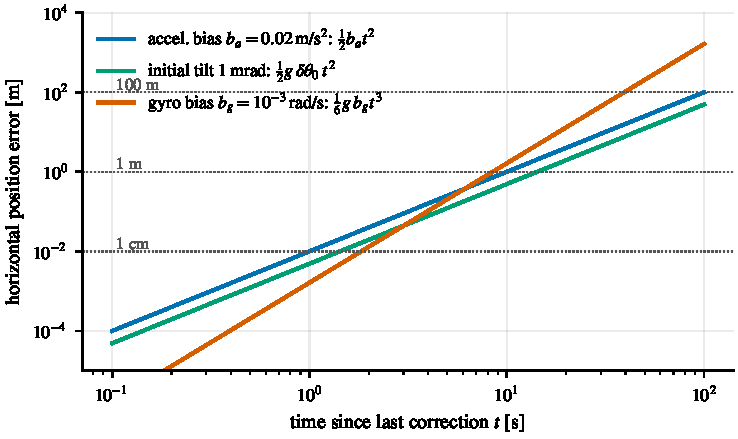
\includegraphics[width=0.86\textwidth]{fig_dr_drift.pdf}
  \caption{Deterministic dead-reckoning drift from three error sources of a consumer-grade IMU.
  A gyro bias of $10^{-3}$~rad/s ($\approx 0.06\,^\circ$/s) produces more than a meter of error
  after ten seconds and hundreds of meters after one minute. The cubic law is why attitude
  accuracy dominates inertial navigation.}
  \label{fig:dr-drift}
\end{figure}

With $b_g = 10^{-3}$~rad/s, a modest value for a MEMS gyroscope, the gyro term alone gives
$1.6$~m after 10~s and $353$~m after 60~s. Random sensor noise adds error that grows in a
similar way. \Cref{ch:errordyn} derives that the position \emph{standard deviation} due to
accelerometer white noise grows as $t^{3/2}$, due to gyroscope white noise as $t^{5/2}$, and due to
the gyroscope bias random walk as $t^{7/2}$.

\begin{keyidea}[inertial navigation is an attitude problem]
Because gravity is large (about $9.81~\mathrm{m/s^2}$) compared with typical accelerometer errors,
a tilt of one milliradian costs as much as an accelerometer bias of about
$10~\mathrm{mm/s^2}$. Position accuracy is therefore limited mostly by attitude accuracy. Any aiding
sensor that constrains roll and pitch, as a camera does, pays off enormously.
\end{keyidea}

\subsection{The camera}

A camera measures the \emph{directions} (bearings) of light rays arriving from the scene. A point
$p_f$ in the world appears in the image at the projection of its camera-frame coordinates
$p_c = (X_c, Y_c, Z_c)$:
\begin{equation}
  z = \begin{bmatrix} X_c/Z_c \\ Y_c/Z_c \end{bmatrix}.
\end{equation}
Because images are measurements of fixed scene geometry, they do not drift the way integrated
inertial data does. But a single camera has a fundamental blind spot.

\begin{proposition}[Monocular scale ambiguity]
\label{prop:scale-ambiguity}
Let a camera with poses $(R_i, p_i)$, $i = 1, \dots, M$, observe points $p_{f,j}$. For any $s > 0$, the
scaled configuration with poses $(R_i, s\,p_i)$ and points $s\,p_{f,j}$ produces exactly the same
images.
\end{proposition}
\begin{proof}
In camera $i$, the scaled point has coordinates
$R_i\T(s\,p_{f,j} - s\,p_i) = s\, R_i\T(p_{f,j} - p_i)$. The projection divides the first two
coordinates by the third, so the factor $s$ cancels.
\end{proof}

A camera alone therefore recovers the trajectory and the scene only up to an unknown global scale.
A photograph of a toy car from 10~cm can be identical to a photograph of a real car from 4~m. Cameras
also fail under motion blur, in darkness, against texture-less surfaces such as white walls, and in
scenes dominated by moving objects.

\subsection{Why the combination works}

\begin{table}[t]
\centering\small
\begin{tabularx}{\textwidth}{@{}>{\raggedright\arraybackslash}X >{\raggedright\arraybackslash}X >{\raggedright\arraybackslash}X@{}}
\toprule
 & \textbf{IMU} & \textbf{Monocular camera} \\
\midrule
Rate & 100--1000 Hz & 10--60 Hz \\
Measures & angular rate, specific force & bearings to scene points \\
Scale & metric & unknown (\cref{prop:scale-ambiguity}) \\
Drift & fast ($t^2$ to $t^3$) & slow, relative to the scene \\
Gravity direction & observable (at rest or on average) & not observable \\
Fails when & always drifts; saturates on impacts & blur, darkness, no texture, pure rotation \\
\bottomrule
\end{tabularx}
\caption{The IMU and the camera fail in complementary ways.}
\label{tab:sensor-complement}
\end{table}

\Cref{tab:sensor-complement} summarizes the complementarity. The camera bounds the inertial drift by
constraining the motion between images. The IMU supplies metric scale, the direction of gravity
(and hence absolute roll and pitch), high-rate motion between frames, and robustness during brief
visual outages. Scale becomes observable because the accelerometer measures acceleration in
$\mathrm{m/s^2}$: scaling a trajectory by $s$ scales its acceleration by $s$, which the
accelerometer would notice. The exception is unaccelerated motion. At constant velocity, the
scale is unobservable again, which is one of several \emph{degenerate motions} studied in
\cref{ch:observability}.

Even fused, four directions remain unobservable: the three components of global position, and the
rotation about the gravity vector (global yaw). Neither sensor senses where the origin is or which
way north is. VIO estimates these relative to the starting pose, and they drift.

\section{Why fusion is hard}

The difficulty of VIO comes from several sources acting at once.
\begin{enumerate}
  \item \textbf{Nonlinearity.} Rotations enter the equations through products and trigonometric
        functions, and the camera projection divides by depth.
  \item \textbf{Curved state spaces.} Orientations do not live in a vector space. You cannot add
        two rotations, and every estimator must deal with this (\cref{ch:lie}).
  \item \textbf{Multi-rate, asynchronous data.} The IMU runs at 200~Hz and the camera at 20~Hz,
        and every measurement must be processed in timestamp order.
  \item \textbf{Unknown scene.} The 3D positions of the visual features are unknown and must be
        estimated, or eliminated, along with the motion.
  \item \textbf{Outliers.} Feature tracks fail, latch onto moving objects, or slide along edges.
  \item \textbf{Unobservability.} Some directions of the state cannot be determined. A careless
        estimator can become falsely confident about them, which is the consistency problem of
        \cref{ch:observability}.
  \item \textbf{Real time.} All of this must run at camera rate, deterministically, on embedded
        processors.
\end{enumerate}

\section{A map of the field}

VIO algorithms differ along three main axes.

\paragraph{Loosely vs.\ tightly coupled.} A loosely coupled system runs a vision-only pipeline
that produces up-to-scale poses and fuses those poses with the IMU. A tightly coupled system feeds
the raw visual measurements (feature positions in the image) directly into a single estimator
together with the inertial data. Tight coupling is more accurate and more robust, because the IMU
helps the vision part and correlations are handled correctly. All modern high-accuracy systems,
and this project, are tightly coupled.

\paragraph{Filtering vs.\ optimization.} \emph{Filtering} approaches (EKF-based) process each
measurement once, keep a Gaussian belief over a bounded state, and discard the past. They are fast
and have predictable cost. \emph{Optimization} approaches solve a nonlinear least-squares problem
over a sliding window of recent states, relinearizing as needed, and summarize discarded states as
a prior (marginalization). They are typically more accurate per frame but more expensive and more
complex. The two families are closer than they appear: the MSCKF is equivalent to a single
Gauss--Newton iteration over a sliding window of poses with the landmarks marginalized
(\cref{ch:msckfupdate}).

\paragraph{Feature-based vs.\ direct.} Feature-based systems extract and track sparse keypoints and
use their image coordinates as measurements. Direct systems use pixel intensities themselves
(photometric error).

\begin{table}[t]
\centering\small
\begin{tabularx}{\textwidth}{@{}l l >{\raggedright\arraybackslash}X@{}}
\toprule
\textbf{System} & \textbf{Family} & \textbf{Notes} \\
\midrule
EKF-SLAM / MonoSLAM~\cite{davison2007monoslam} & filter, landmarks in state & cost grows quadratically with landmarks \\
MSCKF~\cite{mourikis2007msckf, li2013msckf2} & filter, poses in state & landmarks eliminated by nullspace projection; this project \\
MSCKF-VIO~\cite{sun2018msckfvio} & filter (stereo MSCKF) & open-source, fast flight; good engineering reference \\
OpenVINS~\cite{geneva2020openvins} & filter (MSCKF + SLAM features) & research platform with excellent documentation \\
ROVIO~\cite{bloesch2015rovio} & filter, direct & photometric patches in an iterated EKF \\
OKVIS~\cite{leutenegger2015okvis} & optimization, keyframes & sliding-window bundle adjustment \\
VINS-Mono~\cite{qin2018vins} & optimization & preintegration, robust initialization, loop closure \\
ORB-SLAM3~\cite{campos2021orbslam3} & optimization + map & full visual-inertial SLAM with relocalization \\
\bottomrule
\end{tabularx}
\caption{Representative visual-inertial estimators.}
\label{tab:vio-systems}
\end{table}

\section{Why the MSCKF}

In EKF-SLAM every tracked landmark adds three variables to the state. Covariance updates cost
$\mathcal{O}(n^2)$ to $\mathcal{O}(n^3)$ in the state size $n$, so a few hundred landmarks quickly
exhaust a real-time budget, and landmark initialization from a single camera is awkward because
depth is unknown at first sight.

The \textbf{Multi-State Constraint Kalman Filter} of Mourikis and Roumeliotis~\cite{mourikis2007msckf}
keeps instead a sliding window of past IMU poses, called \emph{clones}, taken at image times. When a
feature has been tracked across several clones, its observations constrain those poses relative to
one another. The feature's 3D position is triangulated temporarily, then algebraically
eliminated from the linearized equations by projecting onto the left nullspace of its Jacobian
(\cref{ch:msckfupdate}). The landmark never enters the state. The result:
\begin{itemize}
  \item cost linear in the number of features and bounded by the window size;
  \item no need to initialize landmark depth inside the filter;
  \item all the geometric information of each feature track is used exactly once.
\end{itemize}
These properties make the MSCKF the canonical filter-based VIO and an excellent vehicle for
learning, because it requires every ingredient of the field to be understood and nothing more.

\section{The estimator at a glance}

\begin{figure}[t]
\centering
\begin{tikzpicture}[node distance=7mm and 11mm]
  \node[block] (imu) {IMU\\ \footnotesize 200 Hz};
  \node[block, right=of imu] (prop) {Nominal propagation\\ \footnotesize Ch.~\ref{ch:strapdown}};
  \node[block, right=of prop] (cov) {Covariance propagation\\ \footnotesize Ch.~\ref{ch:errordyn}};
  \node[block, below=10mm of imu] (cam) {Camera\\ \footnotesize 20 Hz};
  \node[block, right=of cam] (front) {Front end: detect,\\ track, reject\\ \footnotesize Ch.~\ref{ch:frontend}};
  \node[block, right=of front] (clone) {Clone pose,\\ augment $P$\\ \footnotesize Ch.~\ref{ch:cloning}};
  \node[block, below=10mm of clone] (upd) {MSCKF update:\\ triangulate, project,\\ gate, update\\ \footnotesize Ch.~\ref{ch:msckfupdate}};
  \node[block, left=of upd] (inj) {Inject, reset,\\ marginalize\\ \footnotesize Ch.~\ref{ch:eskf}, \ref{ch:cloning}};
  \node[block, below=8mm of inj, fill=white] (out) {Pose, velocity,\\ biases, covariance};
  \coordinate (L) at ($(cam.west)+(-7mm,0)$);
  \coordinate (T) at ($(imu.north)+(0,6mm)$);
  \draw[->] (imu) -- (prop);
  \draw[->] (prop) -- (cov);
  \draw[->] (cam) -- (front);
  \draw[->] (front) -- node[note, above]{tracks} (clone);
  \draw[->] (cov) -- (clone);
  \draw[->] (clone) -- (upd);
  \draw[->] (upd) -- (inj);
  \draw[->] (inj) -- (out);
  \draw[->, dashed] (inj.west) -| (L) -- (L |- T) -| node[note, above, pos=0.25]{corrected state feeds back into propagation} (prop.north);
\end{tikzpicture}
\caption{Data flow of the monocular MSCKF built in these notes.}
\label{fig:pipeline}
\end{figure}

\Cref{fig:pipeline} shows the whole estimator. Between images, each IMU sample advances the nominal
state with the nonlinear kinematics and grows the error covariance. When an image arrives, the
filter propagates exactly to the image timestamp, appends a clone of the current pose, and updates
the feature tracks. Tracks that have ended, or whose oldest observation is about to leave the window,
are triangulated and converted into constraints between clones. The update corrects the IMU state and
all clones together, the correction is injected into the nominal state, and the oldest clone is
removed when the window is full. \Cref{ch:planar} builds a complete miniature of this pipeline for a robot moving in a plane,
small enough to derive by hand and to run as a short Python script; it is the place to look whenever the general chapters
feel abstract.

\begin{projectlink}[the road map]
The project builds this pipeline from the bottom up: the Lie group toolkit (M2), the data
stream (M3), inertial propagation (M4--M5), a filter tested against synthetic pose measurements
(M6--M7), the visual front end (M8--M9), and finally the MSCKF (M10a--M10b). Each layer is tested
in isolation before the next is added, so that any later failure can be localized.
\end{projectlink}

\section{The EuRoC benchmark}

The European Robotics Challenge (EuRoC) MAV dataset~\cite{burri2016euroc} is the standard VIO
benchmark. A hexacopter carries a stereo pair of global-shutter cameras ($752 \times 480$, 20~Hz)
and an ADIS16448 MEMS IMU (200~Hz), hardware-synchronized and calibrated. Eleven sequences fly
through an industrial machine hall (MH\_01 to MH\_05) and a motion-capture room (V1\_01 to V2\_03),
graded easy, medium and difficult by speed, lighting and texture. Ground truth comes from a laser
tracker or a motion-capture system. \Cref{app:euroc} documents the file formats and calibration
values the project uses.

\begin{takeaways}
\begin{itemize}
  \item VIO estimates pose, velocity and IMU biases from an IMU and a camera, with no map and no
        absolute positioning, and its error grows without bound.
  \item Inertial drift is dominated by attitude error: a gyro bias produces position error growing
        like $t^3$.
  \item A monocular camera observes the scene only up to scale. The accelerometer supplies the
        scale, provided the body accelerates.
  \item Global position and yaw remain unobservable even with both sensors.
  \item The MSCKF keeps a sliding window of past poses rather than landmarks, which bounds its cost
        while using every feature track.
\end{itemize}
\end{takeaways}

\begin{exercises}
  \item A MEMS accelerometer has a bias of $5~\mathrm{mg}$ ($1\,\mathrm{mg} = 9.81\times10^{-3}~\mathrm{m/s^2}$).
        How long can you dead-reckon before the position error exceeds 1~m? What gyro bias produces
        the same error at the same time?
  \item Prove that the gravity leak produced by a constant tilt error $\delta\theta_0$ is
        $g\,\delta\theta_0$ to first order. What is the exact expression, and at what tilt does the
        first-order formula err by 1\%?
  \item Extend \cref{prop:scale-ambiguity}: show that applying a common rigid transformation
        $(R, t)$ to all camera poses and points also leaves the images unchanged. How many
        unobservable degrees of freedom does a monocular camera have? Which of them does an IMU
        remove, and why?
  \item A drone hovers perfectly still for 30~s. Which states can a VIO system estimate during that
        time, and which cannot be distinguished from each other? (Revisit this after
        \cref{ch:observability}.)
  \item Read the abstract and introduction of~\cite{mourikis2007msckf}. In two sentences, state the
        problem with EKF-SLAM that the paper claims to solve, and the key idea of the solution.
\end{exercises}


\part{Mathematical Foundations}
\chapter{Linear Algebra for State Estimation}
\label{ch:linalg}

\begin{objectives}
\begin{itemize}
  \item Master the cross-product matrix $\sx{a}$ and the identities used in every Jacobian derivation.
  \item Understand the four fundamental subspaces, especially the \emph{left nullspace} on which the
        MSCKF rests.
  \item Know when and why to use Cholesky, LDL$^\mathsf{T}$, QR and SVD, and why a filter should never
        form an explicit inverse.
  \item Use block matrices, Schur complements and the Woodbury identity fluently.
  \item Understand the matrix exponential and floating-point arithmetic well enough to write
        numerically robust code.
\end{itemize}
\end{objectives}

Most of the computation in a Kalman filter is linear algebra: products of covariance matrices,
solutions of linear systems, and factorizations. This chapter collects the tools the rest of the
notes rely on and explains the numerical reasoning behind them. Readers fluent in numerical linear
algebra can skim it, but should not skip \cref{sec:skew,sec:subspaces,sec:floating}.

% ------------------------------------------------------------------------------
\section{Vectors, coordinates and the cross product}
\label{sec:skew}

\subsection{Vectors versus their coordinates}

A physical vector, such as a velocity or the direction of gravity, exists independently of any
coordinate system. To compute with it we express it in a \emph{frame}: an origin plus three
orthonormal, right-handed axes. The same physical vector $\vec{v}$ has different coordinate
triples $v_w \in \R^3$ and $v_b \in \R^3$ in the world and body frames, and the two are related by
a rotation matrix, $v_w = R_{wb}\,v_b$ (\cref{ch:rotations}). Confusing a vector with its
coordinates in some frame is the root of most frame bugs. Throughout these notes, a subscript on a
coordinate vector names the frame it is expressed in.

For coordinate vectors $a, b \in \R^3$ we use the standard inner product
$a\T b = \sum_i a_i b_i$, the Euclidean norm $\|a\| = \sqrt{a\T a}$, and the cross product
$a \times b$. The cross product is bilinear, anti-commutative ($a \times b = -b \times a$), and
orthogonal to both arguments. Its norm is $\|a\|\|b\|\sin\angle(a,b)$.

\subsection{The cross-product (skew-symmetric) matrix}

Because $a \times b$ is linear in $b$, it can be written as a matrix-vector product.

\begin{definition}[Skew-symmetric matrix]
For $a = (a_1, a_2, a_3)\T$, the \emph{cross-product matrix} of $a$ is
\begin{equation}
  \sx{a} = \begin{bmatrix} 0 & -a_3 & a_2 \\ a_3 & 0 & -a_1 \\ -a_2 & a_1 & 0 \end{bmatrix},
  \qquad\text{so that}\qquad \sx{a}\, b = a \times b \quad \forall\, b \in \R^3 .
  \label{eq:skew}
\end{equation}
It is skew-symmetric: $\sx{a}\T = -\sx{a}$. Conversely, every $3\times3$ skew-symmetric matrix
$S$ equals $\sx{s}$ for the unique vector $s = (S_{32}, S_{13}, S_{21})\T$. We write
$s = S\veeop$ for this inverse operation, the \emph{vee} map. In Lie theory, $\sx{\cdot}$ is
also written $(\cdot)\hatop$ and called the \emph{hat} map.
\end{definition}

The following identities are used constantly in derivations. Learn to recognize them on sight.

\begin{proposition}[Cross-product identities]
\label{prop:skew-identities}
For $a, b, c \in \R^3$ and $R \in \SO$ (a rotation matrix):
\begin{align}
  \sx{a}\, b &= -\sx{b}\, a, \label{eq:skew-anticomm}\\
  \sx{a}\, a &= 0, \label{eq:skew-self}\\
  \sx{a}^2 &= a a\T - \|a\|^2 I, \label{eq:skew-sq}\\
  \sx{a}^3 &= -\|a\|^2 \sx{a}, \label{eq:skew-cube}\\
  \sx{a}\sx{b} &= b a\T - (a\T b)\, I, \label{eq:skew-prod}\\
  \sx{a \times b} &= \sx{a}\sx{b} - \sx{b}\sx{a} = b a\T - a b\T, \label{eq:skew-commutator}\\
  \sx{R a} &= R \sx{a} R\T, \label{eq:skew-rot}\\
  R\,(a \times b) &= (Ra) \times (Rb). \label{eq:cross-rot}
\end{align}
\end{proposition}

\begin{proof}
\eqref{eq:skew-anticomm} and \eqref{eq:skew-self} restate $a\times b = -b\times a$ and
$a \times a = 0$. For \eqref{eq:skew-prod}, apply both sides to an arbitrary $c$ and use the
``BAC--CAB'' rule $a \times (b \times c) = b\,(a\T c) - c\,(a\T b)$:
$\sx{a}\sx{b}c = a\times(b\times c) = b a\T c - (a\T b) c$. Setting $b = a$ gives
\eqref{eq:skew-sq}, and multiplying \eqref{eq:skew-sq} by $\sx{a}$ and using \eqref{eq:skew-self}
gives \eqref{eq:skew-cube}. Subtracting \eqref{eq:skew-prod} from its version with $a, b$ swapped
gives the second equality of \eqref{eq:skew-commutator}. The first follows from the Jacobi identity
$a \times (b \times c) + b \times (c \times a) + c \times (a \times b) = 0$. For
\eqref{eq:cross-rot}, the cross product is defined by orientation and lengths, both preserved by a
proper rotation. Finally \eqref{eq:skew-rot} follows from \eqref{eq:cross-rot}:
$\sx{Ra}\, c = (Ra)\times c = (Ra)\times(R R\T c) = R\big(a \times R\T c\big) = R\sx{a}R\T c$.
\end{proof}

\begin{keyidea}[moving a vector out of a cross product]
Identity \eqref{eq:skew-anticomm} is how unknowns are isolated in Jacobian derivations. A
perturbation appears as $\sx{\delta\theta}\,v$, and the Jacobian with respect to $\delta\theta$ is
read off after rewriting it as $-\sx{v}\,\delta\theta$.
\end{keyidea}

Identity \eqref{eq:skew-cube} is what makes closed-form rotation formulas possible: every power of
$\sx{a}$ reduces to a multiple of $\sx{a}$ or $\sx{a}^2$, so infinite series in $\sx{a}$ collapse
to two terms (\cref{ch:rotations}).

% ------------------------------------------------------------------------------
\section{The four fundamental subspaces}
\label{sec:subspaces}

Let $A \in \R^{m\times n}$ have rank $r$. Four subspaces are associated with it:
\begin{center}
\begin{tabular}{@{}l l l l@{}}
\toprule
Subspace & Definition & Lives in & Dimension \\
\midrule
column space (range) & $\range(A) = \{Ax\}$ & $\R^m$ & $r$ \\
nullspace & $\nullsp(A) = \{x : Ax = 0\}$ & $\R^n$ & $n - r$ \\
row space & $\range(A\T)$ & $\R^n$ & $r$ \\
left nullspace & $\nullsp(A\T) = \{y : y\T A = 0\}$ & $\R^m$ & $m - r$ \\
\bottomrule
\end{tabular}
\end{center}

\begin{theorem}[Fundamental theorem of linear algebra]
\label{thm:fundamental}
$\nullsp(A) = \range(A\T)^\perp$ and $\nullsp(A\T) = \range(A)^\perp$. Consequently
$\R^n = \range(A\T) \oplus \nullsp(A)$ and $\R^m = \range(A) \oplus \nullsp(A\T)$, with
orthogonal direct sums.
\end{theorem}
\begin{proof}
$y \in \nullsp(A\T) \iff A\T y = 0 \iff x\T A\T y = 0\ \forall x \iff (Ax)\T y = 0\ \forall x
\iff y \perp \range(A)$. The first statement is the same argument applied to $A\T$.
\end{proof}

The \emph{left nullspace} deserves special attention because the MSCKF is built on it. Suppose a
stacked measurement depends on an unwanted variable $f$ through a tall matrix $H_f \in \R^{m\times
3}$ of full column rank:
\begin{equation}
  r = H_x\,\delta x + H_f\,\delta f + n .
\end{equation}
Take any matrix $A \in \R^{m\times(m-3)}$ whose columns form an orthonormal basis of
$\nullsp(H_f\T)$. Then $A\T H_f = 0$, and multiplying through by $A\T$ gives
$A\T r = A\T H_x\,\delta x + A\T n$: the unwanted variable has disappeared. \Cref{ch:msckfupdate}
shows that no information about $\delta x$ is lost in the process.

\begin{definition}[Orthogonal projector]
A matrix $\Pi$ is an orthogonal projector if $\Pi^2 = \Pi$ and $\Pi\T = \Pi$. If the columns of
$Q$ are an orthonormal basis of a subspace $\mathcal{S}$, the projector onto $\mathcal{S}$ is
$\Pi_{\mathcal{S}} = Q Q\T$. If $A$ has full column rank, the projector onto $\range(A)$ is
$A (A\T A)\inv A\T$, and $I - \Pi_{\mathcal{S}}$ projects onto $\mathcal{S}^\perp$.
\end{definition}

For the matrix $A$ spanning the left nullspace of $H_f$, these facts combine into an identity we
will use to prove the MSCKF's optimality:
\begin{equation}
  A A\T = I - H_f (H_f\T H_f)\inv H_f\T .
  \label{eq:nullspace-projector}
\end{equation}

% ------------------------------------------------------------------------------
\section{Symmetric and positive-definite matrices}

Covariance matrices are symmetric and positive semi-definite, and much of the numerical care in a
filter goes into keeping them that way.

\begin{definition}
A symmetric matrix $P = P\T \in \R^{n\times n}$ is \emph{positive semi-definite} (PSD, $P \succeq 0$) if
$x\T P x \ge 0$ for all $x$, and \emph{positive definite} (PD, $P \succ 0$) if $x\T P x > 0$
for all $x \ne 0$. We write $P_1 \succeq P_2$ (the Loewner order) if $P_1 - P_2 \succeq 0$.
\end{definition}

\begin{theorem}[Spectral theorem]
Every real symmetric matrix factors as $P = U \Lambda U\T$ with $U$ orthogonal and
$\Lambda = \diag(\lambda_1,\dots,\lambda_n)$ real. $P \succeq 0$ if and only if all
$\lambda_i \ge 0$, and $P \succ 0$ if and only if all $\lambda_i > 0$.
\end{theorem}

The geometric picture is an ellipsoid. For $P \succ 0$, the set $\{x : x\T P\inv x \le 1\}$ is an
ellipsoid with principal axes along the columns of $U$ and semi-axis lengths $\sqrt{\lambda_i}$.
This is the ``one-sigma'' uncertainty ellipsoid of a Gaussian with covariance $P$
(\cref{ch:prob}).

\begin{proposition}[Properties of PSD matrices]
\label{prop:psd}
Let $P, Q \succeq 0$ and let $A$ be any matrix of compatible size. Then
\begin{enumerate}
  \item $A P A\T \succeq 0$ (congruence preserves semi-definiteness);
  \item $P + Q \succeq 0$, and $P + Q \succ 0$ if either is PD;
  \item $P_{ii} \ge 0$ and $|P_{ij}| \le \sqrt{P_{ii} P_{jj}}$;
  \item every principal submatrix of $P$ is PSD.
\end{enumerate}
\end{proposition}
\begin{proof}
(1) $x\T A P A\T x = (A\T x)\T P (A\T x) \ge 0$. (2) is immediate. (3) and (4) follow from (1) with
$A$ a selection matrix, using the $2\times2$ determinant for the off-diagonal bound.
\end{proof}

Property (1) explains why the covariance updates $\Phi P \Phi\T + Q$ and the Joseph form
(\cref{ch:kf}) preserve semi-definiteness exactly in exact arithmetic: they are sums of congruences
of PSD matrices. The simpler update $(I - KH)P$ is \emph{not} a congruence, which is why it can lose
positive semi-definiteness under rounding.

% ------------------------------------------------------------------------------
\section{Matrix factorizations}

\subsection{Cholesky and LDL$^\mathsf{T}$}

\begin{theorem}[Cholesky factorization]
A symmetric matrix $S$ is positive definite if and only if $S = L L\T$ for a unique lower
triangular $L$ with positive diagonal.
\end{theorem}

The factor is computed column by column:
\begin{equation}
  L_{jj} = \Big( S_{jj} - \sum_{k<j} L_{jk}^2 \Big)^{1/2}, \qquad
  L_{ij} = \frac{1}{L_{jj}}\Big( S_{ij} - \sum_{k<j} L_{ik}L_{jk} \Big), \quad i > j,
\end{equation}
at a cost of about $n^3/3$ flops, half that of an LU factorization. The algorithm is backward
stable without pivoting, and it fails (a negative argument of the square root) exactly when $S$ is
not numerically positive definite. That makes it a useful diagnostic too. The variant
$S = L D L\T$ with unit-diagonal $L$ and diagonal $D$ avoids square roots, and with symmetric
pivoting (Eigen's \code{LDLT}) it also handles semi-definite matrices gracefully.

Cholesky factors \emph{whiten} correlated quantities. If $n \sim \N(0, S)$ and $S = LL\T$, then
$L\inv n \sim \N(0, I)$. This is how Mahalanobis distances are computed stably:
$r\T S\inv r = \|L\inv r\|^2$, with one triangular solve.

\subsection{QR factorization and Householder reflections}

\begin{definition}[Householder reflection]
For a nonzero $v \in \R^m$, the matrix $H_v = I - 2\, \dfrac{v v\T}{v\T v}$ reflects vectors across
the hyperplane orthogonal to $v$. It is symmetric and orthogonal, $H_v = H_v\T = H_v\inv$.
\end{definition}

Given any $x \in \R^m$, choosing $v = x + \operatorname{sign}(x_1)\|x\|\,e_1$ gives
$H_v x = -\operatorname{sign}(x_1)\|x\|\,e_1$: a single reflection zeroes every entry of $x$ below
the first. (The sign choice avoids cancellation when $x$ is already nearly parallel to $e_1$.)
Applying such reflections to the columns of $A \in \R^{m\times n}$, $m \ge n$, one after another
produces
\begin{equation}
  H_n \cdots H_2 H_1\, A = \begin{bmatrix} R_1 \\ 0 \end{bmatrix}
  \quad\Longleftrightarrow\quad
  A = Q \begin{bmatrix} R_1 \\ 0 \end{bmatrix} = \begin{bmatrix} Q_1 & Q_2 \end{bmatrix}
      \begin{bmatrix} R_1 \\ 0 \end{bmatrix} = Q_1 R_1,
  \label{eq:qr}
\end{equation}
with $Q = H_1 H_2\cdots H_n$ orthogonal, $R_1 \in \R^{n\times n}$ upper triangular, $Q_1 \in
\R^{m\times n}$ and $Q_2 \in \R^{m\times(m-n)}$. The cost is about $2mn^2 - \tfrac23 n^3$ flops.

\begin{proposition}[Nullspaces from QR]
\label{prop:qr-nullspace}
If $A$ has full column rank $n$ and $A = Q_1 R_1$ as in \eqref{eq:qr}, then the columns of $Q_1$
are an orthonormal basis of $\range(A)$ and the columns of $Q_2$ are an orthonormal basis of the
left nullspace $\nullsp(A\T)$. In particular $Q_2\T A = 0$.
\end{proposition}
\begin{proof}
$Q\T A = [R_1;\ 0]$, so $Q_2\T A = 0$. The columns of $Q_2$ are orthonormal and there are $m - n$ of
them, which is the dimension of $\nullsp(A\T)$.
\end{proof}

\begin{implnote}[never form $Q$]
$Q$ is $m\times m$ and dense, but it is defined by only $n$ reflection vectors. Libraries store
those vectors compactly in the lower triangle of the factored matrix. To compute $Q\T B$ for some
other matrix $B$, apply the $n$ reflections to $B$ one at a time, at a cost of $\mathcal{O}(mnk)$
for $B \in \R^{m\times k}$. Forming $Q$ explicitly would cost $\mathcal{O}(m^2 n)$ and $m^2$ storage.
In Eigen, \code{HouseholderQR::householderQ()} returns a lazy \code{HouseholderSequence} that can
be applied to $B$ without materializing $Q$. Whether a particular call allocates must be checked
with the allocation guard, not assumed.
\end{implnote}

A \emph{Givens rotation} zeroes a single entry by rotating two rows. It is the tool of choice when
the matrix is already nearly triangular or very sparse. The original MSCKF paper suggests Givens
rotations for its nullspace projection, because the feature Jacobian has a sparse block structure.

\subsection{The singular value decomposition}

\begin{theorem}[SVD]
Every $A \in \R^{m\times n}$ factors as $A = U \Sigma V\T$ with $U, V$ orthogonal and $\Sigma$
diagonal with entries $\sigma_1 \ge \sigma_2 \ge \dots \ge 0$, the \emph{singular values}.
\end{theorem}

The SVD reveals everything about $A$ at once. The rank is the number of nonzero singular values; the
first $r$ columns of $U$ and $V$ span the column and row spaces, and the remaining columns span the
left nullspace and the nullspace. The \emph{condition number} $\kappa(A) = \sigma_1/\sigma_n$
measures how much relative errors in the data can be amplified in the solution of a linear system.
The minimum-norm least-squares solution of $Ax \approx b$ is $x = A^+ b$ with the pseudo-inverse
$A^+ = V \Sigma^+ U\T$. The SVD is the most robust of the factorizations and also the most
expensive. In this project it appears in the linear triangulation of \cref{ch:multiview} and in
diagnostics.

% ------------------------------------------------------------------------------
\section{Solving linear systems and least squares}

\begin{pitfall}[explicit inverses]
Formulas such as $K = P H\T S\inv$ are notation, not algorithms. Computing $S\inv$ and then
multiplying costs about three times as much as solving, is less accurate, and destroys structure.
Factor $S$ once (Cholesky or LDL$^\mathsf{T}$) and solve: $S K\T = H P\T$ gives $K\T$ by two
triangular substitutions per column. Writing \code{S.ldlt().solve(Identity)} is still an explicit
inverse in disguise.
\end{pitfall}

\paragraph{Least squares.} Given an overdetermined system $Ax \approx b$ with $A \in \R^{m\times n}$
of full column rank, the least-squares solution minimizes $\|Ax - b\|^2$. Setting the gradient to zero
gives the \emph{normal equations} $A\T A x = A\T b$. They are cheap but square the condition number,
$\kappa(A\T A) = \kappa(A)^2$, which can lose half the significant digits. The QR approach is more
stable: with $A = Q_1R_1$, $\|Ax - b\|^2 = \|R_1 x - Q_1\T b\|^2 + \|Q_2\T b\|^2$, so
$x = R_1\inv Q_1\T b$ by back substitution, and the residual norm is $\|Q_2\T b\|$.

\paragraph{Weighted least squares.} If the errors have covariance $W$, minimize
$(Ax - b)\T W\inv (Ax - b)$. With $W = LL\T$ this is ordinary least squares on the whitened system
$L\inv A x \approx L\inv b$.

% ------------------------------------------------------------------------------
\section{Block matrices and the Schur complement}

Estimation constantly partitions vectors and matrices into blocks: IMU state versus clones, poses
versus landmarks. Block elimination is the basic tool.

\begin{proposition}[Block factorization and inverse]
\label{prop:block-inverse}
Let $M = \begin{bmatrix} A & B \\ C & D \end{bmatrix}$ with $A$ invertible, and define the
\emph{Schur complement} of $A$ in $M$, $M/A := D - C A\inv B$. Then
\begin{equation}
  M = \begin{bmatrix} I & 0 \\ C A\inv & I \end{bmatrix}
      \begin{bmatrix} A & 0 \\ 0 & M/A \end{bmatrix}
      \begin{bmatrix} I & A\inv B \\ 0 & I \end{bmatrix},
  \qquad \det M = \det A \cdot \det(M/A),
\end{equation}
and if $M/A$ is invertible,
\begin{equation}
  M\inv = \begin{bmatrix}
    A\inv + A\inv B\, (M/A)\inv\, C A\inv & -A\inv B\, (M/A)\inv \\
    -(M/A)\inv C A\inv & (M/A)\inv
  \end{bmatrix}.
\end{equation}
\end{proposition}
\begin{proof}
Multiply out the three factors. The inverse is the product of the inverses of the three factors in
reverse order, and the inverses of the unit-triangular block factors are obtained by negating their
off-diagonal blocks.
\end{proof}

For a symmetric $M$ with $A \succ 0$: $M \succ 0$ if and only if $M/A \succ 0$. The Schur
complement is the algebraic form of \emph{eliminating} a block of variables. \Cref{ch:prob} shows it
is exactly Gaussian marginalization in information form and conditioning in covariance form.

\begin{theorem}[Woodbury matrix identity]
\label{thm:woodbury}
For invertible $A$ and $C$ and conformable $U, V$,
\begin{equation}
  (A + U C V)\inv = A\inv - A\inv U \big( C\inv + V A\inv U \big)\inv V A\inv .
\end{equation}
\end{theorem}
\begin{proof}
Write the block matrix $\begin{bmatrix} A & U \\ V & -C\inv\end{bmatrix}$ and compute the
top-left block of its inverse in two ways with \cref{prop:block-inverse}: eliminating $A$ first gives
the right-hand side, and eliminating $-C\inv$ first gives $(A + UCV)\inv$.
\end{proof}

Woodbury connects the two forms of the Kalman update (\cref{ch:kf}). It says that a low-rank update
of a matrix gives a low-rank update of its inverse, which is why an update with $m$ measurements
needs only an $m\times m$ inverse no matter how large the state is.

% ------------------------------------------------------------------------------
\section{The matrix exponential}
\label{sec:matexp}

\begin{definition}
For $A \in \R^{n\times n}$, $\exp(A) = \sum_{k=0}^\infty \frac{A^k}{k!} = I + A + \tfrac12 A^2 + \tfrac16 A^3 + \cdots$.
The series converges absolutely for every $A$.
\end{definition}

\begin{proposition}[Properties of the matrix exponential]
\label{prop:matexp}
\begin{enumerate}
  \item $x(t) = \exp(tA)\, x_0$ is the unique solution of $\dot x = Ax$, $x(0) = x_0$.
  \item $\frac{\dd}{\dd t}\exp(tA) = A \exp(tA) = \exp(tA)\, A$.
  \item $\exp(A)\inv = \exp(-A)$, and $\det\exp(A) = e^{\tr A}$.
  \item $\exp(T A T\inv) = T \exp(A)\, T\inv$ for invertible $T$.
  \item If $AB = BA$ then $\exp(A + B) = \exp(A)\exp(B)$. \textbf{In general this fails.}
\end{enumerate}
\end{proposition}

The failure of property 5 for non-commuting matrices is the algebraic root of everything subtle
about rotations: two rotations generated by $\sx{a}$ and $\sx{b}$ do not compose into the rotation
generated by $\sx{a + b}$. \Cref{ch:lie} measures the discrepancy precisely.

\begin{example}[Nilpotent generator: the double integrator]
\label{ex:double-integrator}
For $F = \begin{bmatrix} 0 & 1 \\ 0 & 0 \end{bmatrix}$, $F^2 = 0$, so the series terminates:
$\exp(F\Dt) = \begin{bmatrix} 1 & \Dt \\ 0 & 1\end{bmatrix}$. This is the exact transition matrix of
position and velocity under zero acceleration. The inertial error dynamics of \cref{ch:errordyn}
have a similar nilpotent structure, so their exponentials can be written in closed form.
\end{example}

% ------------------------------------------------------------------------------
\section{Derivatives and Jacobians}

\begin{definition}[Jacobian layout]
For $f: \R^n \to \R^m$, the Jacobian $\frac{\partial f}{\partial x} \in \R^{m\times n}$ has
entries $\big[\frac{\partial f}{\partial x}\big]_{ij} = \frac{\partial f_i}{\partial x_j}$
(numerator layout), so that $f(x + \delta) = f(x) + \frac{\partial f}{\partial x}\delta +
o(\|\delta\|)$. Column $j$ is the sensitivity of the output to the $j$-th input direction. This
is exactly what a finite-difference test computes column by column.
\end{definition}

With this layout the chain rule reads
$\frac{\partial (g\circ f)}{\partial x} = \frac{\partial g}{\partial y}\big|_{y = f(x)}\frac{\partial f}{\partial x}$,
a product of matrices in the same order as the composition. A few derivatives recur:
\begin{equation}
  \frac{\partial (Ax)}{\partial x} = A, \qquad
  \frac{\partial (a \times x)}{\partial x} = \sx{a}, \qquad
  \frac{\partial (x \times a)}{\partial x} = -\sx{a}, \qquad
  \frac{\partial (x\T S x)}{\partial x} = x\T (S + S\T).
\end{equation}
\Cref{ch:lie} extends Jacobians to functions whose inputs or outputs are rotations.

% ------------------------------------------------------------------------------
\section{Floating-point arithmetic}
\label{sec:floating}

An IEEE~754 \code{double} stores a sign, an 11-bit exponent, and a 53-bit significand (52 stored
bits plus an implicit leading one). Two constants matter:
\begin{itemize}
  \item the \emph{machine epsilon} $\mach = 2^{-52} \approx 2.22\times10^{-16}$, the gap between $1$
        and the next larger double (\code{std::numeric\_limits<double>::epsilon()});
  \item the \emph{unit roundoff} $u = 2^{-53} \approx 1.11\times10^{-16}$: every basic operation
        satisfies $\mathrm{fl}(a \circ b) = (a\circ b)(1 + \delta)$ with $|\delta| \le u$.
\end{itemize}
Relative accuracy is therefore excellent for a single operation. Trouble comes from
\emph{cancellation}: subtracting two nearly equal numbers that each carry a rounding error leaves
a small result whose relative error can be enormous.

\begin{example}[Catastrophic cancellation in $1 - \cos\theta$]
\label{ex:cancellation}
For $\theta = 10^{-5}$, $\cos\theta = 1 - 5\times10^{-11} + \dots$. The stored value of
$\cos\theta$ has an absolute error up to $u \approx 10^{-16}$, so $1 - \cos\theta \approx
5\times 10^{-11}$ is computed with relative error up to $10^{-16}/(5\times10^{-11}) \approx 2\times
10^{-6}$. Dividing by $\theta^2$ to form $(1-\cos\theta)/\theta^2 \approx 1/2$ keeps that relative
error. At $\theta = 10^{-8}$, $\cos\theta$ rounds to exactly $1$, and the computed value is $0$
instead of $1/2$. The Taylor expansion $\tfrac12 - \tfrac{\theta^2}{24} + \cdots$ has no
cancellation at all. \Cref{fig:taylor} in \cref{ch:lie} shows this effect for all the coefficient
functions of the rotation group.
\end{example}

\begin{pitfall}[time stamps in floating point]
EuRoC timestamps are nanoseconds since the Unix epoch, about $1.4\times10^{18}$, which lies between
$2^{60}$ and $2^{61}$. A \code{double} near that value can only represent multiples of
$2^{60-52} = 256$~ns. Converting absolute timestamps to \code{double} therefore quantizes them to
256~ns, and accumulating time by repeated addition of $\Dt$ drifts further. Keep absolute time in
64-bit integers (\code{std::chrono::nanoseconds}) and convert only differences to \code{double}
(AGENTS.md C5).
\end{pitfall}

\paragraph{Finite-difference step size.} A finite-difference derivative is itself a cancellation.
For the central difference $\frac{f(x+h) - f(x-h)}{2h}$, the truncation error is about
$\frac{h^2}{6}|f'''|$ and the rounding error about $\frac{u |f|}{h}$. Their sum is minimized at
\begin{equation}
  h^\star = \left(\frac{3\,u\,|f|}{|f'''|}\right)^{1/3} \approx 10^{-5}\text{ to }10^{-6}
  \quad\text{(for quantities of order one)},
\end{equation}
with a total error of order $u^{2/3} \approx 10^{-11}$. For the one-sided difference the optimal step
is $\sim\sqrt{u} \approx 10^{-8}$ and the error is only $\sim 10^{-8}$. This is why Jacobian tests
use central differences with $h \approx 10^{-6}$ and tolerances around $10^{-6}$ to $10^{-8}$, scaled
to the magnitude of the quantities involved.

\paragraph{Conditioning versus stability.} A problem is \emph{ill-conditioned} if small changes in
its data produce large changes in its exact answer. An algorithm is \emph{unstable} if it produces
much larger errors than the conditioning of the problem justifies. Computing the rotation angle
from a rotation matrix with $\arccos$ near zero angle is an unstable algorithm for a
well-conditioned problem (\cref{ch:lie}). Triangulating a point seen with almost no parallax is an
ill-conditioned problem that no algorithm can rescue (\cref{ch:multiview}).

\begin{takeaways}
\begin{itemize}
  \item $\sx{a}b = a\times b = -\sx{b}a$, $\sx{a}^3 = -\|a\|^2\sx{a}$, and $\sx{Ra} = R\sx{a}R\T$ are
        the workhorses of every rotation derivation.
  \item The left nullspace of a tall matrix is the orthogonal complement of its column space.
        A full QR factorization delivers an orthonormal basis for it.
  \item Covariance updates should be congruences ($APA\T$) plus PSD terms, so that positive
        semi-definiteness is preserved structurally.
  \item Factor and solve; never form an explicit inverse, and never form $Q$ explicitly.
  \item Schur complements eliminate variables; Woodbury converts between large and small inverses.
  \item Cancellation, not single operations, destroys floating-point accuracy. Time stamps belong
        in 64-bit integers.
\end{itemize}
\end{takeaways}

\begin{exercises}
  \item Prove \eqref{eq:skew-commutator} directly from \eqref{eq:skew-prod}, and verify the Jacobi
        identity numerically for random vectors.
  \item Show that the eigenvalues of $\sx{a}$ are $0$ and $\pm i\|a\|$. Which eigenvector belongs to $0$?
  \item Let $H_f \in \R^{2M\times3}$ have full column rank. Compute the dimension of its left
        nullspace for $M = 2, 3, 10$. Prove \eqref{eq:nullspace-projector}.
  \item Show that if $P\succ0$ then $P - K S K\T \succeq 0$ for $S = HPH\T + R$, $K = PH\T S\inv$
        and $R \succ 0$. (Hint: Schur complement of a suitable $2\times2$ block matrix.)
  \item Implement Householder QR in Python for a $10\times3$ matrix and check
        \cref{prop:qr-nullspace} numerically. Then compare the accuracy of solving a least-squares
        problem with $\kappa(A) = 10^8$ by the normal equations and by QR.
  \item Use \cref{thm:woodbury} to show that
        $\big(P\inv + H\T R\inv H\big)\inv = P - PH\T(HPH\T + R)\inv HP$. Which side is cheaper to
        evaluate when $P$ is $75\times75$ and $R$ is $2\times2$? When $R$ is $500\times500$?
  \item What is the spacing of doubles near $2^{30}$ seconds expressed in nanoseconds? Would storing
        time as \code{double} seconds since the epoch be acceptable for a 200~Hz IMU?
  \item For $f(x) = \sin x$ at $x = 1$, plot the error of forward and central differences versus
        $h \in [10^{-16}, 10^{-1}]$ on log axes and locate the optimal step sizes. Compare with the
        formulas above.
\end{exercises}

\chapter{Numerical Linear Algebra}
\label{ch:numlinalg}

\begin{objectives}
\begin{itemize}
  \item Count the cost of matrix operations and understand why a filter must never form an explicit inverse.
  \item Derive the LU, Cholesky, QR and singular value decompositions, and know which one to use when.
  \item Solve least-squares problems stably, and compute nullspaces, projectors and pseudo-inverses.
  \item Use block matrices, Schur complements and the Woodbury identity fluently.
  \item Understand the matrix exponential, and why the exponential of a skew-symmetric matrix is a rotation.
  \item Understand floating-point arithmetic: rounding, cancellation, conditioning and stability.
\end{itemize}
\end{objectives}

\Cref{ch:linalg} described what matrices \emph{are}. This chapter is about computing with them reliably. A Kalman filter
spends nearly all of its time in a few operations: multiplying matrices, solving linear systems with a covariance matrix,
and factorizing Jacobians. Done naively, these operations are slow, lose accuracy, or silently destroy the symmetry and
positive definiteness of covariances. Done well, they are fast and accurate to nearly machine precision.

% ==============================================================================
\section{The cost of matrix operations}

Numerical analysts count \term{flops} (floating-point operations: one addition or multiplication each). Some basic costs
for $n\times n$ matrices:
\begin{center}\small
\begin{tabular}{@{}l l@{}}
\toprule
Operation & Approximate flops \\
\midrule
dot product of two $n$-vectors & $2n$ \\
matrix-vector product & $2n^2$ \\
matrix-matrix product & $2n^3$ \\
solving a triangular system & $n^2$ \\
LU factorization & $\tfrac23n^3$ \\
Cholesky factorization & $\tfrac13n^3$ \\
explicit inverse & $2n^3$ \\
\bottomrule
\end{tabular}
\end{center}
For the MSCKF with $n = 75$, a matrix product costs about $8\times10^5$ flops, a fraction of a millisecond. Costs grow with the cube of
the dimension, which is why filters keep their state small, exploit block structure, and update only the blocks that change.
We write $\mathcal{O}(n^3)$ (``order $n^3$'') to mean ``at most a constant times $n^3$ for large $n$''.

% ==============================================================================
\section{Triangular systems and the LU factorization}

\subsection{Forward and back substitution}

A triangular system is solved by direct substitution. For an upper-triangular $U$ with non-zero diagonal, the last equation
$U_{nn}x_n = b_n$ gives $x_n$, the previous one then gives $x_{n-1}$, and so on:
\begin{equation}
  x_i = \frac{1}{U_{ii}}\Big(b_i - \sum_{j>i}U_{ij}x_j\Big), \qquad i = n, n-1, \dots, 1 .
\end{equation}
This is \term{back substitution}; \emph{forward substitution} solves lower-triangular systems from the top. Each costs about $n^2$
flops. Every method in this chapter reduces a hard problem to one or two triangular solves.

\subsection{LU factorization}

Gaussian elimination (\cref{sec:linsys}) subtracts multiples $\ell_{ik}$ of row $k$ from the rows below it, column by column, until
the matrix is upper triangular. Recording the multipliers in a unit lower-triangular matrix $L$ gives the \term{LU factorization}
\begin{equation}
  A = LU .
\end{equation}
Then $Ax = b$ is solved by forward substitution $Ly = b$ and back substitution $Ux = y$. The factorization costs $\tfrac23n^3$ flops
once; every additional right-hand side costs only $2n^2$.

\paragraph{Pivoting.} Elimination divides by the pivots. A tiny pivot creates huge multipliers that amplify rounding errors.
The classic example is $\begin{bmatrix}10^{-20} & 1\\ 1 & 1\end{bmatrix}$: eliminating with the pivot $10^{-20}$ gives a multiplier
of $10^{20}$, and in double precision the computed solution of $Ax = (1, 2)$ is completely wrong, although the matrix is
perfectly well conditioned. Swapping the two rows first fixes it. \emph{Partial pivoting} always swaps the row with the largest
available pivot into place, giving $PA = LU$ with a permutation matrix $P$. Symmetric positive-definite matrices, which is
what filters mostly factor, need no pivoting at all, as the next section shows.

% ==============================================================================
\section{The Cholesky factorization}

\begin{theorem}[Cholesky factorization]
\label{thm:cholesky}
\index{Cholesky factorization}
A symmetric matrix $S$ is positive definite if and only if $S = LL\T$ for a lower-triangular $L$ with positive diagonal.
This $L$ is unique.
\end{theorem}
\begin{proof}
If $S = LL\T$ with $L$ invertible, then $x\T Sx = \|L\T x\|^2 > 0$ for $x \ne 0$. Conversely, partition
\begin{equation*}
  S = \begin{bmatrix} s_{11} & s\T \\ s & S_{22} \end{bmatrix}
    = \begin{bmatrix} \ell_{11} & 0 \\ \ell & L_{22} \end{bmatrix}\begin{bmatrix} \ell_{11} & \ell\T \\ 0 & L_{22}\T \end{bmatrix}
    = \begin{bmatrix} \ell_{11}^2 & \ell_{11}\ell\T \\ \ell_{11}\ell & \ell\ell\T + L_{22}L_{22}\T \end{bmatrix}.
\end{equation*}
Matching blocks: $\ell_{11} = \sqrt{s_{11}}$ (positive because $s_{11} = e_1\T Se_1 > 0$), $\ell = s/\ell_{11}$, and
$L_{22}L_{22}\T = S_{22} - ss\T/s_{11}$. The last matrix (a Schur complement, \cref{sec:schur}) is again positive definite, so the
construction continues recursively on a matrix one size smaller. Each step is forced, which proves uniqueness.
\end{proof}

Unrolling the recursion column by column gives the algorithm
\begin{equation}
  L_{jj} = \Big( S_{jj} - \sum_{k<j} L_{jk}^2 \Big)^{1/2}, \qquad
  L_{ij} = \frac{1}{L_{jj}}\Big( S_{ij} - \sum_{k<j} L_{ik}L_{jk} \Big), \quad i > j,
\end{equation}
at a cost of $\tfrac13n^3$ flops, half that of LU. The algorithm is backward stable without pivoting, and it fails (the argument
of a square root is not positive) exactly when $S$ is not numerically positive definite, which makes it a useful diagnostic
too. The variant $S = LDL\T$, with unit-diagonal $L$ and diagonal $D$, avoids square roots; with symmetric pivoting (Eigen's
\code{LDLT}) it also handles semi-definite and slightly indefinite matrices gracefully.

\paragraph{Uses of the Cholesky factor.}
\begin{itemize}
  \item \emph{Solving} $Sx = b$: forward-substitute $Ly = b$, back-substitute $L\T x = y$.
  \item \emph{Whitening}: if a random vector $n$ has covariance $S = LL\T$, then $L\inv n$ has covariance $I$ (\cref{ch:prob}).
        Mahalanobis distances are computed as $r\T S\inv r = \|L\inv r\|^2$ with a single triangular solve.
  \item \emph{Sampling}: if $s$ has covariance $I$, then $Ls$ has covariance $S$.
  \item \emph{Determinants}: $\det S = \prod_iL_{ii}^2$, and $\log\det S = 2\sum_i\log L_{ii}$ without overflow.
\end{itemize}

% ==============================================================================
\section{Orthogonal factorizations: QR}

Orthogonal transformations do not amplify errors (they preserve lengths), so factorizations built from them are the most
stable available.

\subsection{QR from Gram--Schmidt}

Applying Gram--Schmidt to the columns $a_1, \dots, a_n$ of a full-column-rank $A \in \R^{m\times n}$ produces orthonormal $q_1, \dots, q_n$
with $a_k = \sum_{j\le k}r_{jk}q_j$, where $r_{jk} = q_j\T a_k$ and $r_{kk} = \|\tilde q_k\|$. In matrix form
\begin{equation}
  A = Q_1R_1, \qquad Q_1 = [q_1 \cdots q_n] \in \R^{m\times n},\quad Q_1\T Q_1 = I,\quad R_1 \text{ upper triangular}.
\end{equation}
This is the \term{QR factorization}. Classical Gram--Schmidt, implemented literally, loses orthogonality in floating point when the
columns are nearly dependent; the computed $q$'s drift away from being orthogonal. Householder reflections avoid this problem.

\subsection{Householder reflections}

\begin{definition}[Householder reflection]
\index{Householder reflection}
For a non-zero $v \in \R^m$, the matrix $H_v = I - 2\, \dfrac{v v\T}{v\T v}$ reflects vectors across the hyperplane orthogonal to $v$:
it reverses the component along $v$ and leaves the orthogonal components unchanged. It is symmetric and orthogonal, and is its own
inverse: $H_v = H_v\T = H_v\inv$.
\end{definition}

\begin{proposition}[Zeroing a vector below its first entry]
For $x \in \R^m$ not a multiple of $e_1$, let $\alpha = -\operatorname{sign}(x_1)\|x\|$ and $v = x - \alpha e_1$. Then $H_vx = \alpha e_1$.
\end{proposition}
\begin{proof}
Because $\|x\| = \|\alpha e_1\|$, the vectors $x$ and $\alpha e_1$ have the same length, so the reflection across the
perpendicular bisector of the segment joining them swaps them. That bisecting hyperplane is orthogonal to $v = x - \alpha e_1$.
Algebraically: $v\T v = 2\|x\|^2 - 2\alpha x_1$ and $v\T x = \|x\|^2 - \alpha x_1 = \tfrac12v\T v$, so
$H_vx = x - 2v\,\frac{v\T x}{v\T v} = x - v = \alpha e_1$.
\end{proof}

The sign choice makes $v_1 = x_1 + \operatorname{sign}(x_1)\|x\|$ a sum of two numbers of the same sign, avoiding the cancellation
that the other choice would suffer when $x$ is nearly parallel to $e_1$.

\paragraph{Householder QR.} Apply a reflection $H_1$ that zeroes the first column of $A$ below the diagonal; then a reflection $H_2$,
acting on rows $2, \dots, m$, that zeroes the second column below the diagonal; and so on for all $n$ columns:
\begin{equation}
  H_n \cdots H_2 H_1\, A = \begin{bmatrix} R_1 \\ 0 \end{bmatrix}
  \quad\Longleftrightarrow\quad
  A = Q \begin{bmatrix} R_1 \\ 0 \end{bmatrix} = \begin{bmatrix} Q_1 & Q_2 \end{bmatrix}
      \begin{bmatrix} R_1 \\ 0 \end{bmatrix} = Q_1 R_1,
  \label{eq:qr}
\end{equation}
with $Q = H_1 H_2\cdots H_n$ orthogonal ($m\times m$), $R_1 \in \R^{n\times n}$ upper triangular, $Q_1 \in \R^{m\times n}$ and $Q_2 \in \R^{m\times(m-n)}$. The
cost is about $2mn^2 - \tfrac23 n^3$ flops. The form $A = Q[R_1; 0]$ is the \emph{full} QR factorization, and $A = Q_1R_1$ the
\emph{thin} one.

\paragraph{Applying $Q\T$ without forming $Q$.} Each $H_k$ is determined by its vector $v_k$, so $Q\T b = H_n\cdots H_1b$ is computed by
applying the reflections one at a time:
\begin{equation}
  b \;\gets\; b - v_k\,\frac{2\,v_k\T b}{v_k\T v_k}, \qquad k = 1, \dots, n,
\end{equation}
at a cost of $\mathcal{O}(m)$ per reflection. Forming $Q$ explicitly would cost $\mathcal{O}(m^2n)$ flops and $m^2$ storage.

\begin{proposition}[Nullspaces from QR]
\label{prop:qr-nullspace}
If $A$ has full column rank $n$ and $A = Q_1 R_1$ as in \eqref{eq:qr}, then the columns of $Q_1$ are an orthonormal basis of
$\range(A)$ and the columns of $Q_2$ are an orthonormal basis of the left nullspace $\nullsp(A\T)$. In particular $Q_2\T A = 0$.
\end{proposition}
\begin{proof}
$Q\T A = [R_1;\ 0]$, so $Q_2\T A = 0$, i.e.\ the columns of $Q_2$ lie in $\nullsp(A\T)$. They are orthonormal and there are $m - n$ of them,
which is the dimension of $\nullsp(A\T)$ by rank--nullity. Since $R_1$ is invertible, $\range(A) = \range(Q_1)$.
\end{proof}

\begin{implnote}[never form $Q$]
Libraries store the Householder vectors compactly in the lower triangle of the factored matrix. In Eigen,
\code{HouseholderQR::householderQ()} returns a lazy \code{HouseholderSequence} that can be applied to another matrix without
materializing $Q$. This is exactly what the MSCKF needs: it applies the reflections that triangularize a feature Jacobian to the
rest of the measurement equations (\cref{ch:msckfupdate}). Whether a particular call allocates must be checked with the allocation
guard, not assumed.
\end{implnote}

\subsection{Givens rotations}

A \term{Givens rotation} zeroes one entry at a time by rotating a pair of rows. To zero $b$ in the pair $(a, b)$, set
$r = \sqrt{a^2 + b^2}$, $c = a/r$ and $s = b/r$:
\begin{equation}
  \begin{bmatrix} c & s \\ -s & c \end{bmatrix}\begin{bmatrix} a \\ b \end{bmatrix} = \begin{bmatrix} r \\ 0 \end{bmatrix}.
\end{equation}
Embedded in an identity matrix, it acts on two rows of a larger matrix and leaves the others untouched. Givens rotations are
preferred when only a few entries need to be zeroed, when the matrix is sparse, or when rows arrive one at a time. The original
MSCKF paper suggests them for its nullspace projection, because the feature Jacobian has a sparse block structure.

% ==============================================================================
\section{Least squares}
\label{sec:least-squares}

\subsection{The problem and the normal equations}

An overdetermined system $Ax \approx b$, with $A \in \R^{m\times n}$, $m > n$, generally has no exact solution. The \term{least-squares}
solution minimizes the squared residual
\begin{equation}
  f(x) = \|Ax - b\|^2 = x\T A\T Ax - 2x\T A\T b + b\T b .
\end{equation}
Setting the gradient $2A\T Ax - 2A\T b$ to zero gives the \term{normal equations}
\begin{equation}
  A\T A\,x = A\T b .
  \label{eq:normal-equations}
\end{equation}
If $A$ has full column rank, $A\T A$ is positive definite (since $x\T A\T Ax = \|Ax\|^2 > 0$ for $x\ne0$), so the solution is unique and is
a minimum.

\paragraph{Geometric meaning.} The normal equations say $A\T(b - Ax) = 0$: the residual is orthogonal to every column of $A$. The fitted
vector $Ax$ is the orthogonal projection of $b$ onto $\range(A)$, the closest point to $b$ that the model can produce.

\begin{definition}[Orthogonal projector]
\index{projector}
A matrix $\Pi$ is an orthogonal projector if $\Pi^2 = \Pi$ and $\Pi\T = \Pi$. If the columns of $Q$ are an orthonormal basis of a subspace
$\mathcal{S}$, the projector onto $\mathcal{S}$ is $\Pi_{\mathcal{S}} = QQ\T$. For $A$ of full column rank the projector onto $\range(A)$ is
$A(A\T A)\inv A\T$, and $I - \Pi$ projects onto the orthogonal complement.
\end{definition}

Combining the two descriptions of the projector onto $\range(A)$, and recalling that the columns of $Q_2$ in \eqref{eq:qr} span its
complement $\nullsp(A\T)$, gives an identity we will use to prove the optimality of the MSCKF: for any $A_\perp$ whose columns are an
orthonormal basis of the left nullspace of a full-column-rank $H_f$,
\begin{equation}
  A_\perp A_\perp\T = I - H_f (H_f\T H_f)\inv H_f\T .
  \label{eq:nullspace-projector}
\end{equation}

\subsection{Three ways to solve}

\paragraph{Cholesky on the normal equations.} Form $A\T A$ ($mn^2$ flops) and factor it. This is the fastest method, but forming
$A\T A$ squares the condition number of the problem (\cref{sec:conditioning}): $\kappa(A\T A) = \kappa(A)^2$. When $\kappa(A) = 10^8$,
the normal equations lose essentially all sixteen significant digits.

\paragraph{QR.} With $A = Q[R_1; 0]$ and the invariance of lengths under $Q\T$,
\begin{equation}
  \|Ax - b\|^2 = \|Q\T(Ax - b)\|^2 = \|R_1x - Q_1\T b\|^2 + \|Q_2\T b\|^2 .
\end{equation}
The second term does not depend on $x$, and the first vanishes for $x = R_1\inv Q_1\T b$, computed by back substitution. The minimum
residual is $\|Q_2\T b\|$. This method works with the condition number of $A$ itself and is the standard choice.

\paragraph{SVD.} The most robust and most expensive method, required when $A$ may be rank deficient (\cref{sec:svd}).

\subsection{Weighted least squares}

When the equations have different reliabilities, with errors of covariance $W$, the right objective weights each residual by its
uncertainty (\cref{ch:estimation}):
\begin{equation}
  \min_x\ (Ax - b)\T W\inv(Ax - b) .
\end{equation}
With $W = LL\T$ this is ordinary least squares on the \emph{whitened} system $L\inv Ax \approx L\inv b$, and the normal equations become
$A\T W\inv A\,x = A\T W\inv b$.

% ==============================================================================
\section{The singular value decomposition}
\label{sec:svd}

\begin{theorem}[Singular value decomposition]
\label{thm:svd}
\index{singular value decomposition}
Every $A \in \R^{m\times n}$ can be written as $A = U\Sigma V\T$ with $U \in \R^{m\times m}$ and $V \in \R^{n\times n}$ orthogonal and
$\Sigma \in \R^{m\times n}$ diagonal with entries $\sigma_1 \ge \sigma_2 \ge \dots \ge 0$, the \term{singular values}.
\end{theorem}
\begin{proof}[Construction]
$A\T A$ is symmetric and PSD, so by the spectral theorem $A\T A = V\Lambda V\T$ with orthonormal $v_i$ and eigenvalues
$\lambda_1 \ge \dots \ge \lambda_n \ge 0$. Set $\sigma_i = \sqrt{\lambda_i}$. For each $\sigma_i > 0$ define $u_i = Av_i/\sigma_i$. These are
orthonormal: $u_i\T u_j = v_i\T A\T Av_j/(\sigma_i\sigma_j) = \lambda_jv_i\T v_j/(\sigma_i\sigma_j) = \delta_{ij}$. Complete them to an
orthonormal basis $u_1, \dots, u_m$ of $\R^m$. Then $Av_i = \sigma_iu_i$ for all $i$ (for $\sigma_i = 0$, $\|Av_i\|^2 = \lambda_i = 0$),
which in matrix form is $AV = U\Sigma$.
\end{proof}

\begin{figure}[t]
  \centering
  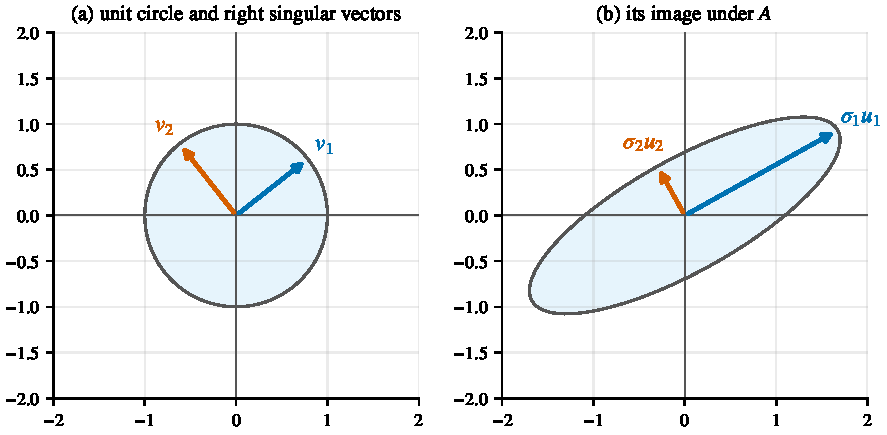
\includegraphics[width=0.9\textwidth]{fig_svd_geometry.pdf}
  \caption{Geometry of the SVD of a $2\times2$ matrix. The right singular vectors $v_1, v_2$ (left) form an orthonormal basis that $A$ maps
  to orthogonal vectors $\sigma_1u_1, \sigma_2u_2$ (right). The unit circle becomes an ellipse with semi-axes $\sigma_1$ and $\sigma_2$: every
  linear map is a rotation, an axis-aligned scaling, and another rotation.}
  \label{fig:svd}
\end{figure}

The SVD says that every linear map, in suitable orthonormal bases of its domain and codomain, is a pure scaling (\cref{fig:svd}). It
reveals everything about $A$ at once:
\begin{itemize}
  \item the rank $r$ is the number of non-zero singular values;
  \item $u_1, \dots, u_r$ span $\range(A)$, $u_{r+1}, \dots, u_m$ span $\nullsp(A\T)$, $v_1, \dots, v_r$ span $\range(A\T)$ and
        $v_{r+1}, \dots, v_n$ span $\nullsp(A)$;
  \item $\|A\|_2 = \sigma_1$ and $\|A\|_F^2 = \sum_i\sigma_i^2$.
\end{itemize}

\paragraph{Pseudo-inverse.} The \term{pseudo-inverse} $A^+ = V\Sigma^+U\T$, where $\Sigma^+$ inverts the non-zero singular values and transposes
the shape, gives the minimum-norm least-squares solution $x = A^+b$ of any system, including rank-deficient ones. For full column
rank, $A^+ = (A\T A)\inv A\T$.

\begin{proposition}[Homogeneous least squares]
\label{prop:homogeneous-ls}
\index{homogeneous least squares}
The unit vector $x$ minimizing $\|Ax\|$ is the right singular vector $v_n$ belonging to the smallest singular value, and the minimum is
$\sigma_n$.
\end{proposition}
\begin{proof}
$\|Ax\|^2 = x\T A\T Ax$, and by the Rayleigh quotient (\cref{prop:rayleigh}) its minimum over unit vectors is the smallest eigenvalue of
$A\T A$, $\sigma_n^2$, attained at the corresponding eigenvector $v_n$.
\end{proof}

Many geometric estimation problems have the form $Ax = 0$ with $x$ known only up to scale: estimating an essential matrix or a homography
from correspondences, or triangulating a point in homogeneous coordinates (\cref{ch:multiview}). With noisy data there is no exact
solution, and \cref{prop:homogeneous-ls} gives the best one.

\begin{theorem}[Best low-rank approximation, Eckart--Young]
\index{Eckart--Young theorem}
Among all matrices of rank at most $k$, the one closest to $A$ in the Frobenius or 2-norm is $A_k = \sum_{i\le k}\sigma_iu_iv_i\T$, obtained by
zeroing all but the $k$ largest singular values.
\end{theorem}

This is how an estimated matrix is projected onto a set defined by its singular values: for example, the nearest valid essential matrix to a
noisy estimate is obtained by replacing its singular values by $(1, 1, 0)$ (\cref{ch:multiview}).

% ==============================================================================
\section{Conditioning and stability}
\label{sec:conditioning}

Two different things can make a computed answer inaccurate: the problem itself may be sensitive to its data, or the algorithm may add more
error than necessary.

\begin{definition}[Condition number]
\index{condition number}
For an invertible (or full-column-rank) $A$, $\kappa(A) = \sigma_{\max}/\sigma_{\min} = \|A\|_2\,\|A^+\|_2$.
\end{definition}

\begin{proposition}[Sensitivity of linear systems]
If $Ax = b$ and $A(x + \delta x) = b + \delta b$, then $\dfrac{\|\delta x\|}{\|x\|} \le \kappa(A)\,\dfrac{\|\delta b\|}{\|b\|}$.
\end{proposition}
\begin{proof}
$\delta x = A\inv\delta b$ gives $\|\delta x\| \le \|A\inv\|\|\delta b\|$, and $b = Ax$ gives $\|b\| \le \|A\|\|x\|$. Multiply the two
inequalities.
\end{proof}

A problem with condition number $\kappa$ can lose about $\log_{10}\kappa$ significant digits whatever the algorithm; it is
\emph{ill-conditioned} when $\kappa$ is large. An algorithm is \emph{backward stable} if its computed answer is the exact answer to a
problem whose data differ from the true data by a few units of rounding error; such an algorithm never loses more than the
conditioning dictates. Householder QR, Cholesky on positive-definite matrices and LU with partial pivoting are backward stable in
practice; classical Gram--Schmidt and the normal equations for ill-conditioned least squares are not. In geometric terms:
triangulating a point seen with almost no parallax is an ill-conditioned problem that no algorithm can rescue
(\cref{ch:multiview}), while recovering the rotation angle from a rotation matrix with $\arccos$ is an unstable algorithm for a
well-conditioned problem (\cref{ch:lie}).

\begin{pitfall}[explicit inverses]
Formulas such as $K = P H\T S\inv$ are notation, not algorithms. Computing $S\inv$ and then multiplying costs about three times as much as
solving, is less accurate, and destroys structure. Factor $S$ once (Cholesky or LDL$^\mathsf{T}$) and solve: $S K\T = H P\T$ gives $K\T$
by two triangular substitutions per column. Writing \code{S.ldlt().solve(Identity)} is still an explicit inverse in disguise.
\end{pitfall}

% ==============================================================================
\section{Block matrices and the Schur complement}
\label{sec:schur}

Estimation constantly partitions vectors and matrices into blocks: IMU state versus clones, poses versus landmarks. Block elimination is
the basic tool.

\begin{proposition}[Block factorization and inverse]
\label{prop:block-inverse}
\index{Schur complement}
Let $M = \begin{bmatrix} A & B \\ C & D \end{bmatrix}$ with $A$ invertible, and define the \term{Schur complement} of $A$ in $M$,
$M/A := D - C A\inv B$. Then
\begin{equation}
  M = \begin{bmatrix} I & 0 \\ C A\inv & I \end{bmatrix}
      \begin{bmatrix} A & 0 \\ 0 & M/A \end{bmatrix}
      \begin{bmatrix} I & A\inv B \\ 0 & I \end{bmatrix},
  \qquad \det M = \det A \cdot \det(M/A),
\end{equation}
and if $M/A$ is invertible,
\begin{equation}
  M\inv = \begin{bmatrix}
    A\inv + A\inv B\, (M/A)\inv\, C A\inv & -A\inv B\, (M/A)\inv \\
    -(M/A)\inv C A\inv & (M/A)\inv
  \end{bmatrix}.
\end{equation}
\end{proposition}
\begin{proof}
Multiply out the three factors. The inverse is the product of the inverses of the three factors in reverse order, and the inverse of a
unit block-triangular factor is obtained by negating its off-diagonal block.
\end{proof}

The Schur complement is what remains of the equations for the second block of unknowns after the first block has been eliminated. To see
this, solve $\begin{bmatrix}A & B\\C & D\end{bmatrix}\begin{bmatrix}x\\y\end{bmatrix} = \begin{bmatrix}f\\g\end{bmatrix}$ by eliminating
$x = A\inv(f - By)$ from the second equation: $(D - CA\inv B)\,y = g - CA\inv f$. For symmetric $M$ with $A \succ 0$, $M \succ 0$ if and only if
$M/A \succ 0$. \Cref{ch:prob} shows that the Schur complement is exactly Gaussian conditioning in covariance form and marginalization in
information form, and \cref{ch:nlls} uses it to eliminate landmarks from bundle adjustment.

\begin{theorem}[Woodbury matrix identity]
\label{thm:woodbury}
\index{Woodbury identity}
For invertible $A$ and $C$ and conformable $U, V$,
\begin{equation}
  (A + U C V)\inv = A\inv - A\inv U \big( C\inv + V A\inv U \big)\inv V A\inv .
\end{equation}
\end{theorem}
\begin{proof}
Write the block matrix $M = \begin{bmatrix} A & U \\ V & -C\inv\end{bmatrix}$ and compute the top-left block of $M\inv$ in two ways with
\cref{prop:block-inverse}. Eliminating $A$ first gives $A\inv + A\inv U(-C\inv - VA\inv U)\inv VA\inv$, the right-hand side. Eliminating the
bottom-right block $-C\inv$ first (the same proposition with the roles of the blocks exchanged) gives the inverse of its Schur complement,
$(A - U(-C\inv)\inv V)\inv = (A + UCV)\inv$.
\end{proof}

Woodbury connects the two forms of the Kalman update (\cref{ch:kf}). It says that a low-rank update of a matrix gives a low-rank update of
its inverse, which is why an update with $m$ measurements needs only an $m\times m$ inverse no matter how large the state is. Its
determinant counterpart is the \emph{matrix determinant lemma} $\det(A + UCV) = \det(C\inv + VA\inv U)\det C\det A$.

% ==============================================================================
\section{The matrix exponential}
\label{sec:matexp}

\begin{definition}[Matrix exponential]
\index{matrix exponential}
For $A \in \R^{n\times n}$, $\exp(A) = \sum_{k=0}^\infty \frac{A^k}{k!} = I + A + \tfrac12 A^2 + \tfrac16 A^3 + \cdots$.
\end{definition}

The series converges for every $A$: the norm of the $k$-th term is at most $\|A\|^k/k!$, and $\sum_k\|A\|^k/k! = e^{\|A\|}$ is finite.

\begin{proposition}[Properties of the matrix exponential]
\label{prop:matexp}
\begin{enumerate}
  \item $\frac{\dd}{\dd t}\exp(tA) = A \exp(tA) = \exp(tA)\, A$.
  \item $x(t) = \exp(tA)\, x_0$ is the unique solution of $\dot x = Ax$, $x(0) = x_0$ (\cref{ch:calculus}).
  \item If $AB = BA$ then $\exp(A + B) = \exp(A)\exp(B)$. \textbf{In general this fails.}
  \item $\exp(A)\inv = \exp(-A)$, and $\exp(A\T) = \exp(A)\T$.
  \item $\exp(T A T\inv) = T \exp(A)\, T\inv$ for invertible $T$.
  \item $\det\exp(A) = e^{\tr A}$.
\end{enumerate}
\end{proposition}
\begin{proof}
(1) Differentiate the series term by term: $\frac{\dd}{\dd t}\frac{t^kA^k}{k!} = A\frac{t^{k-1}A^{k-1}}{(k-1)!}$.
(3) When $A$ and $B$ commute, the binomial theorem holds for $(A + B)^k$, and the Cauchy product of the two series reproduces the series of
$\exp(A + B)$, exactly as for numbers. (4) $A$ and $-A$ commute, so $\exp(A)\exp(-A) = \exp(0) = I$; transposing the series term by term
gives the second statement. (5) $(TAT\inv)^k = TA^kT\inv$. (6) For diagonalizable $A = V\Lambda V\inv$, (5) gives
$\exp(A) = V\exp(\Lambda)V\inv$ with $\exp(\Lambda) = \diag(e^{\lambda_i})$, so $\det\exp(A) = \prod_ie^{\lambda_i} = e^{\sum\lambda_i} = e^{\tr A}$;
the general case follows by continuity, since diagonalizable matrices are dense. Statement (2) is proved in \cref{ch:calculus}.
\end{proof}

The failure of property 3 for non-commuting matrices is the algebraic root of everything subtle about rotations: two rotations generated
by $\sx{a}$ and $\sx{b}$ do not compose into the rotation generated by $\sx{a + b}$. \Cref{ch:lie} measures the discrepancy precisely.

\begin{proposition}[Exponentials of skew-symmetric matrices are rotations]
\label{prop:exp-skew}
If $S\T = -S$ then $\exp(S)$ is a rotation matrix.
\end{proposition}
\begin{proof}
By property 4, $\exp(S)\T\exp(S) = \exp(S\T)\exp(S) = \exp(-S)\exp(S) = I$, so $\exp(S)$ is orthogonal; and
$\det\exp(S) = e^{\tr S} = e^0 = 1$ because a skew-symmetric matrix has a zero diagonal.
\end{proof}

This little proposition is the bridge between the flat world of vectors and the curved world of rotations: every vector $\phi \in \R^3$
defines the rotation $\exp(\sx{\phi})$, and \cref{ch:rotations,ch:lie} show that every rotation arises this way.

\paragraph{Computing the exponential.}
\begin{itemize}
  \item \emph{Nilpotent matrices} ($A^k = 0$ for some $k$): the series is a finite sum.
  \item \emph{Diagonalizable matrices}: $\exp(A) = V\diag(e^{\lambda_i})V\inv$.
  \item \emph{Structured matrices}: when powers of $A$ repeat, as for skew-symmetric $3\times3$ matrices, the series can be summed in closed form
        (Rodrigues' formula, \cref{ch:rotations}).
  \item \emph{General matrices}: \emph{scaling and squaring}. Choose $s$ such that $\|A\|/2^s$ is small, approximate $\exp(A/2^s)$ by a
        truncated series or a rational (Pad\'e) approximation, and square the result $s$ times, using $\exp(A) = \exp(A/2^s)^{2^s}$. This is what
        library routines such as \code{scipy.linalg.expm} do.
\end{itemize}

\begin{example}[Nilpotent generator: the double integrator]
\label{ex:double-integrator}
For $F = \begin{bmatrix} 0 & 1 \\ 0 & 0 \end{bmatrix}$, $F^2 = 0$, so the series terminates:
$\exp(F\Dt) = \begin{bmatrix} 1 & \Dt \\ 0 & 1\end{bmatrix}$. This is the exact transition matrix of position and velocity under zero
acceleration. The inertial error dynamics of \cref{ch:errordyn} have a similar nilpotent structure, so their exponentials can be written in
closed form.
\end{example}

% ==============================================================================
\section{Floating-point arithmetic}
\label{sec:floating}

\subsection{Representation}

\index{floating point}
An IEEE~754 \code{double} represents a number as $\pm1.f\times2^e$, with a sign bit, an 11-bit exponent $e$ and a 52-bit fraction $f$ (53
significant bits counting the implicit leading one). Its range is about $10^{-308}$ to $10^{308}$; results beyond the range \emph{overflow}
to $\pm\infty$, and results below it \emph{underflow} gradually to zero. Undefined operations such as $0/0$ or $\infty - \infty$ produce
\code{NaN} (``not a number''), which propagates through every subsequent operation and compares unequal to everything, including itself.
A single \code{NaN} in a covariance matrix contaminates the whole filter within one update.

\subsection{Rounding}

Two constants describe the precision:
\begin{itemize}
  \item the \term{machine epsilon} $\mach = 2^{-52} \approx 2.22\times10^{-16}$, the gap between $1$ and the next larger double
        (\code{std::numeric\_limits<double>::epsilon()});
  \item the \emph{unit roundoff} $u = 2^{-53} \approx 1.11\times10^{-16}$: every basic operation satisfies
        $\mathrm{fl}(a \circ b) = (a\circ b)(1 + \delta)$ with $|\delta| \le u$.
\end{itemize}
The spacing between consecutive doubles is proportional to their magnitude: near $x$ it is about $\mach|x|$. Relative accuracy is therefore
excellent for a single operation. Errors accumulate in long computations (a sum of $n$ terms can carry a relative error of order $nu$ in the
worst case, though typically $\sqrt n\,u$), but the dramatic losses come from \emph{cancellation}.

\subsection{Cancellation}

Subtracting two nearly equal numbers, each carrying a relative rounding error of size $u$, produces a small result whose \emph{absolute}
error is still of size $u$ times the operands, so its \emph{relative} error can be enormous. The subtraction itself is exact; it merely
exposes the errors already present.

\begin{example}[Catastrophic cancellation in $1 - \cos\theta$]
\label{ex:cancellation}
For $\theta = 10^{-5}$, $\cos\theta = 1 - 5\times10^{-11} + \dots$. The stored value of $\cos\theta$ has an absolute error up to
$u \approx 10^{-16}$, so $1 - \cos\theta \approx 5\times 10^{-11}$ is computed with relative error up to $10^{-16}/(5\times10^{-11}) \approx 2\times
10^{-6}$. Dividing by $\theta^2$ to form $(1-\cos\theta)/\theta^2 \approx 1/2$ keeps that relative error. At $\theta = 10^{-8}$, $\cos\theta$ rounds
to exactly $1$, and the computed value is $0$ instead of $1/2$. The Taylor expansion $\tfrac12 - \tfrac{\theta^2}{24} + \cdots$ has no
cancellation at all. \Cref{fig:taylor} in \cref{ch:lie} shows this effect for all the coefficient functions of the rotation group.
\end{example}

The remedies are always the same: rewrite the expression to avoid the subtraction (for example
$1 - \cos\theta = 2\sin^2(\theta/2)$), use a series expansion in the dangerous regime, or reorganize the algorithm (for example
\code{atan2} instead of \code{acos} for angles, \cref{ch:lie}).

\begin{pitfall}[time stamps in floating point]
EuRoC timestamps are nanoseconds since the Unix epoch, about $1.4\times10^{18}$, which lies between $2^{60}$ and $2^{61}$. A \code{double} near
that value can only represent multiples of $2^{60-52} = 256$~ns. Converting absolute timestamps to \code{double} therefore quantizes them to
256~ns, and accumulating time by repeated addition of $\Dt$ drifts further. Keep absolute time in 64-bit integers
(\code{std::chrono::nanoseconds}) and convert only differences to \code{double} (AGENTS.md C5).
\end{pitfall}

\begin{takeaways}
\begin{itemize}
  \item Costs grow as $n^3$; exploit structure and update only what changes.
  \item Cholesky ($S = LL\T$) is the factorization of choice for covariances: half the cost of LU, stable without pivoting, and a built-in test
        of positive definiteness.
  \item Householder QR is the stable way to solve least squares and to obtain orthonormal bases of a column space and of its complement,
        the left nullspace. Apply $Q\T$ through its reflections; never form $Q$.
  \item The SVD reveals rank, nullspaces and conditioning, and solves homogeneous least squares $\min\|Ax\|$, $\|x\| = 1$.
  \item Schur complements eliminate variables; Woodbury converts between large and small inverses.
  \item $\exp(A + B) \neq \exp(A)\exp(B)$ unless $A$ and $B$ commute; the exponential of a skew-symmetric matrix is a rotation.
  \item Cancellation, not single operations, destroys floating-point accuracy. Time stamps belong in 64-bit integers.
\end{itemize}
\end{takeaways}

\begin{exercises}
  \item Solve $\begin{bmatrix}10^{-20} & 1\\ 1 & 1\end{bmatrix}x = \begin{bmatrix}1\\2\end{bmatrix}$ in double precision by elimination without
        pivoting and with partial pivoting. Explain the difference.
  \item Compute the Cholesky factor of $\begin{bmatrix}4 & 2 & 2\\ 2 & 5 & 3\\ 2 & 3 & 6\end{bmatrix}$ by hand and use it to solve $Sx = (8, 10, 11)$.
  \item Show that if $P\succ0$ then $P - K S K\T \succeq 0$ for $S = HPH\T + R$, $K = PH\T S\inv$ and $R \succ 0$. (Hint: the Schur complement of
        $\begin{bmatrix}S & HP\\ PH\T & P\end{bmatrix}$.)
  \item Implement Householder QR in Python for a $10\times3$ matrix, check \cref{prop:qr-nullspace} numerically, and compare the accuracy of solving
        a least-squares problem with $\kappa(A) = 10^8$ by the normal equations and by QR.
  \item Prove \eqref{eq:nullspace-projector} using a full QR factorization of $H_f$.
  \item Use \cref{thm:woodbury} to show that $\big(P\inv + H\T R\inv H\big)\inv = P - PH\T(HPH\T + R)\inv HP$. Which side is cheaper to evaluate when
        $P$ is $75\times75$ and $R$ is $2\times2$? When $R$ is $500\times500$?
  \item Compute $\exp\big(\begin{bmatrix}0 & -\theta\\ \theta & 0\end{bmatrix}\big)$ by summing the series, and recognize the result.
  \item Show that for $A = \begin{bmatrix}0 & 1\\0 & 0\end{bmatrix}$ and $B = \begin{bmatrix}0 & 0\\1 & 0\end{bmatrix}$,
        $\exp(A + B) \ne \exp(A)\exp(B)$.
  \item What is the spacing of doubles near $2^{30}$ seconds expressed in nanoseconds? Would storing time as \code{double} seconds since the epoch
        be acceptable for a 200~Hz IMU?
  \item Rewrite $\sqrt{x^2 + 1} - x$ for large $x$ and $(1 - \cos x)/x^2$ for small $x$ so that they are computed accurately.
\end{exercises}

\chapter{Calculus, Differential Equations and Numerical Integration}
\label{ch:calculus}
\chaptermark{Calculus and ODEs} % short running header

\begin{objectives}
\begin{itemize}
  \item Use partial derivatives, gradients, Jacobians and Hessians, and the chain rule in matrix form.
  \item Use Taylor's theorem with explicit error terms; this is what ``linearization'' and ``first order'' mean.
  \item Differentiate common matrix expressions: inverses, quadratic forms, determinants.
  \item Solve linear ordinary differential equations, including time-varying ones, with the state transition matrix.
  \item Integrate differential equations numerically, predict the order of the error, and verify it.
  \item Compute derivatives numerically with a step size chosen from first principles.
\end{itemize}
\end{objectives}

A navigation filter is a differential equation (the vehicle's motion) integrated numerically from noisy derivatives (the IMU
readings), corrected with linearized measurement models. This chapter collects the calculus behind those three activities:
derivatives and linearization, differential equations and their solutions, and the numerical methods that approximate both.

% ==============================================================================
\section{Derivatives of functions of several variables}

\subsection{Partial derivatives, gradients and Jacobians}

For a scalar function $f(x_1, \dots, x_n)$, the \emph{partial derivative} $\partial f/\partial x_j$ is the ordinary derivative with respect to
$x_j$ with the other variables held fixed. The \term{gradient} collects them:
$\nabla f = (\partial f/\partial x_1, \dots, \partial f/\partial x_n)\T$. For a vector function $f: \R^n \to \R^m$ the partial derivatives form the
\term{Jacobian} matrix.

\begin{definition}[Jacobian, numerator layout]
For $f: \R^n \to \R^m$, the Jacobian $\frac{\partial f}{\partial x} \in \R^{m\times n}$ has entries
$\big[\frac{\partial f}{\partial x}\big]_{ij} = \frac{\partial f_i}{\partial x_j}$. Row $i$ is the gradient of the $i$-th output (transposed); column $j$ is
the sensitivity of all outputs to the $j$-th input.
\end{definition}

The Jacobian is the matrix of the best linear approximation of $f$ near $x$:
\begin{equation}
  f(x + \delta) = f(x) + \frac{\partial f}{\partial x}\,\delta + o(\|\delta\|),
  \label{eq:linearization}
\end{equation}
where $o(\|\delta\|)$ denotes a remainder that goes to zero faster than $\|\delta\|$. Column $j$ is exactly what a finite-difference
test computes by perturbing the $j$-th input (\cref{sec:numdiff}).

\begin{proposition}[Chain rule]
\label{prop:chain-rule}
\index{chain rule}
If $y = f(x)$ and $z = g(y)$, then $\dfrac{\partial z}{\partial x} = \dfrac{\partial g}{\partial y}\Big|_{y = f(x)}\,\dfrac{\partial f}{\partial x}$.
\end{proposition}
\begin{proof}
Substitute the linear approximation of $f$ into that of $g$:
$g(f(x + \delta)) = g\big(f(x) + J_f\delta + o(\|\delta\|)\big) = g(f(x)) + J_gJ_f\delta + o(\|\delta\|)$.
\end{proof}

With the numerator layout the factors appear in the same order as the composition $g\circ f$, which makes long chains easy to write: the
Jacobian of a camera measurement with respect to a pose is ``(projection) times (frame change) times (pose perturbation)''
(\cref{ch:msckfupdate}).

The \term{Hessian} of a scalar function is the matrix of second derivatives, $[\nabla^2f]_{ij} = \partial^2f/\partial x_i\partial x_j$. For smooth $f$ it is
symmetric. It describes curvature: the second-order behavior of $f$ near a point.

\subsection{Taylor's theorem}

\begin{theorem}[Taylor's theorem in one variable]
\label{thm:taylor}
\index{Taylor's theorem}
If $f$ has $n + 1$ continuous derivatives, then
\begin{equation}
  f(x + h) = \sum_{k=0}^n\frac{f^{(k)}(x)}{k!}h^k + \frac{f^{(n+1)}(\xi)}{(n+1)!}h^{n+1}
\end{equation}
for some $\xi$ between $x$ and $x + h$ (Lagrange form of the remainder).
\end{theorem}

The theorem says more than ``$f$ is close to its Taylor polynomial'': it bounds the error. If $|f^{(n+1)}| \le M$ on the interval, the
error of the degree-$n$ polynomial is at most $Mh^{n+1}/(n+1)!$. This is how we will judge every approximation in these notes.

\begin{figure}[t]
  \centering
  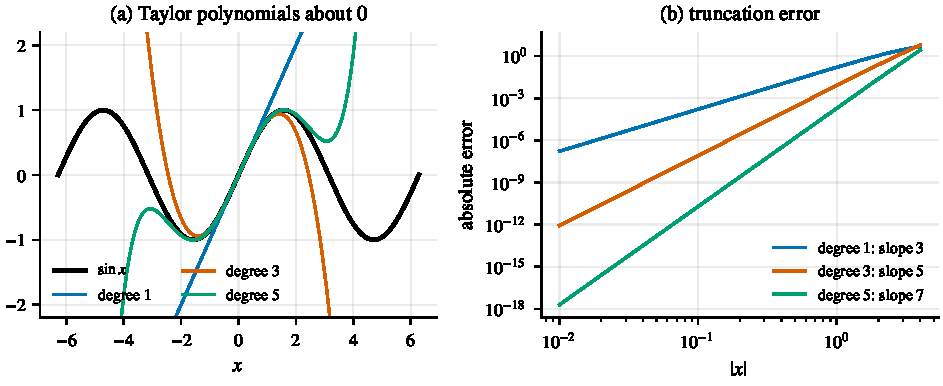
\includegraphics[width=0.95\textwidth]{fig_taylor_sin.pdf}
  \caption{Taylor polynomials of $\sin x$ about $0$ (left) and the absolute error of each (right, log-log scale). Near the expansion point the
  error of the degree-$n$ polynomial falls like $|x|^{n+1}$ or faster. Because the even-order terms of $\sin x$ vanish, the polynomials of degree 1, 3
  and 5 coincide with those of degree 2, 4 and 6, and their errors fall like $|x|^3$, $|x|^5$ and $|x|^7$ (slopes 3, 5 and 7). Far from the
  expansion point, every truncated series fails.}
  \label{fig:taylor-sin}
\end{figure}

\paragraph{Big-O and little-o.} We write $g(h) = O(h^p)$ if $|g(h)| \le Ch^p$ for some constant $C$ as $h\to0$, and $g(h) = o(h^p)$ if
$g(h)/h^p \to 0$. An approximation is \emph{first-order accurate} if its error is $O(h^2)$: the error of a linearization shrinks
quadratically with the size of the perturbation. ``Keeping terms to first order'' in a derivation means writing the result as
linear terms plus an $O(\|\delta\|^2)$ remainder, and then dropping the remainder.

For functions of several variables, Taylor's theorem to second order reads
\begin{equation}
  f(x + \delta) = f(x) + \nabla f(x)\T\delta + \tfrac12\delta\T\nabla^2f(x)\,\delta + O(\|\delta\|^3),
\end{equation}
and for vector functions each component expands this way. The size of the second-order term relative to the first measures how good a
linearization is: when uncertainties are small compared with the scale over which the Jacobian changes, linearization is accurate.
This is the quantitative content of the statement that an extended Kalman filter works well when errors are small (\cref{ch:nonlinear}).

\subsection{Matrix calculus}

A few derivatives recur throughout estimation. We write them as differentials ($\dd f$ = the linear change of $f$ for a small change of the
argument):
\begin{align}
  \dd(Ax) &= A\,\dd x, & \frac{\partial (Ax)}{\partial x} &= A, \\
  \dd(x\T Ax) &= x\T(A + A\T)\,\dd x, & \nabla_x(x\T Ax) &= (A + A\T)x \ \ (= 2Ax \text{ if } A \text{ symmetric}), \\
  \dd(a\times x) &= \sx{a}\,\dd x, & \dd(x \times a) &= -\sx{a}\,\dd x, \\
  \dd(A\inv) &= -A\inv(\dd A)A\inv, & \dd\log\det A &= \tr(A\inv\dd A) .
\end{align}
\begin{proof}[Derivations]
The first and third lines are linear maps, their own derivatives. For the quadratic form,
$(x + \dd x)\T A(x + \dd x) - x\T Ax = \dd x\T Ax + x\T A\,\dd x + O(\|\dd x\|^2) = x\T(A\T + A)\dd x + O(\|\dd x\|^2)$. For the inverse,
differentiate $AA\inv = I$: $(\dd A)A\inv + A\,\dd(A\inv) = 0$. For the log-determinant of a positive-definite $A = U\Lambda U\T$, a small
change $\dd A$ changes each eigenvalue by $u_i\T(\dd A)u_i$ to first order, so
$\dd\sum_i\log\lambda_i = \sum_iu_i\T(\dd A)u_i/\lambda_i = \tr(U\Lambda\inv U\T\dd A) = \tr(A\inv\dd A)$.
\end{proof}

\subsection{Stationary points}

A smooth function has a local minimum at $x^\star$ only if $\nabla f(x^\star) = 0$, and it does have one if, in addition,
$\nabla^2f(x^\star) \succ 0$: by the second-order Taylor expansion, $f(x^\star + \delta) - f(x^\star) = \tfrac12\delta\T\nabla^2f\,\delta + O(\|\delta\|^3) > 0$
for small $\delta \neq 0$. Every least-squares problem in these notes is solved by setting a gradient to zero; \cref{ch:nlls} develops the
iterative methods needed when the resulting equations are nonlinear.

% ==============================================================================
\section{Ordinary differential equations}

\subsection{What a differential equation is}

An \term{ordinary differential equation} (ODE) in state-space form is
\begin{equation}
  \dot x(t) = f\big(x(t), t\big), \qquad x(t_0) = x_0,
\end{equation}
where $x(t) \in \R^n$ is the \emph{state} and $\dot x = \dd x/\dd t$. Any higher-order equation can be put in this form by adding derivatives to
the state: Newton's law $\ddot p = a$ becomes the first-order system $\dot p = v$, $\dot v = a$ with state $(p, v)$. The kinematics of a
navigating vehicle are exactly such a system, with the IMU supplying the right-hand side.

\begin{theorem}[Existence and uniqueness, Picard--Lindel\"of]
\index{Picard--Lindel\"of theorem}
If $f$ is continuous in $t$ and Lipschitz continuous in $x$ (there is an $L$ with $\|f(x, t) - f(y, t)\| \le L\|x - y\|$), the initial value
problem has a unique solution on some interval around $t_0$.
\end{theorem}

Uniqueness is what makes prediction possible: the present state and the inputs determine the future. All the systems in these notes are
smooth enough for the theorem to apply. (A non-example is $\dot x = \sqrt{|x|}$, $x(0) = 0$, solved both by $x \equiv 0$ and by $x = t^2/4$.)

\subsection{Scalar linear equations}

The scalar equation $\dot x = ax + b(t)$ is solved with an \emph{integrating factor}. Multiplying by $e^{-at}$ gives
$\frac{\dd}{\dd t}\big(e^{-at}x\big) = e^{-at}b(t)$; integrating from $t_0$ to $t$,
\begin{equation}
  x(t) = e^{a(t - t_0)}x_0 + \int_{t_0}^t e^{a(t - s)}\,b(s)\,\dd s .
\end{equation}
The solution is the free response of the initial condition plus a weighted sum of the inputs, each propagated from the time it was applied.
Every linear system has this structure.

\subsection{Linear time-invariant systems}

\begin{theorem}[Solution of linear time-invariant systems]
\label{thm:lti-solution}
The solution of $\dot x = Ax + Bu(t)$, $x(t_0) = x_0$, is
\begin{equation}
  x(t) = e^{A(t - t_0)}x_0 + \int_{t_0}^t e^{A(t - s)}Bu(s)\,\dd s .
  \label{eq:lti-solution}
\end{equation}
In particular $\dot x = Ax$ has the unique solution $x(t) = e^{A(t - t_0)}x_0$.
\end{theorem}
\begin{proof}
By \cref{prop:matexp}, $\frac{\dd}{\dd t}\big(e^{-At}x\big) = e^{-At}(\dot x - Ax) = e^{-At}Bu$. Integrating from $t_0$ to $t$ and multiplying by $e^{At}$ gives
\eqref{eq:lti-solution}. The same computation shows that \emph{any} solution satisfies \eqref{eq:lti-solution}, which proves uniqueness.
\end{proof}

The matrix $e^{A\Dt}$ propagates the state over an interval $\Dt$. If $A = V\Lambda V\inv$, the solution is a combination of modes
$e^{\lambda_it}$: decaying for $\operatorname{Re}\lambda_i < 0$, growing for $\operatorname{Re}\lambda_i > 0$, oscillating for imaginary parts. Error
dynamics of inertial navigation have eigenvalues at zero, so their errors grow polynomially rather than exponentially
(\cref{ch:errordyn}).

\subsection{Linear time-varying systems and the state transition matrix}

When the system matrix changes with time, $\dot x = A(t)x$, the exponential no longer applies directly, but its key property survives.

\begin{definition}[State transition matrix]
\index{state transition matrix}
The \term{state transition matrix} $\Phi(t, s)$ of $\dot x = A(t)x$ is the solution of the matrix equation
$\frac{\partial}{\partial t}\Phi(t, s) = A(t)\Phi(t, s)$ with $\Phi(s, s) = I$.
\end{definition}

\begin{proposition}[Properties of the state transition matrix]
\label{prop:stm}
\begin{enumerate}
  \item $x(t) = \Phi(t, s)\,x(s)$ for every solution: $\Phi$ maps states at time $s$ to states at time $t$.
  \item $\Phi(t, s)\,\Phi(s, r) = \Phi(t, r)$ (the semigroup property) and $\Phi(t, s)\inv = \Phi(s, t)$.
  \item For constant $A$, $\Phi(t, s) = e^{A(t - s)}$.
  \item If $A(t)$ commutes with $A(s)$ for all $t, s$, then $\Phi(t, s) = \exp\big(\int_s^tA(\tau)\,\dd\tau\big)$. In general this formula is
        \emph{wrong}.
  \item The solution of $\dot x = A(t)x + B(t)u(t)$ is $x(t) = \Phi(t, t_0)x_0 + \int_{t_0}^t\Phi(t, s)B(s)u(s)\,\dd s$.
\end{enumerate}
\end{proposition}
\begin{proof}
(1) Both $x(t)$ and $\Phi(t, s)x(s)$ solve the ODE with the same value at $t = s$; by uniqueness they agree. (2) Both sides of the first
identity, as functions of $t$, solve the matrix ODE with the value $\Phi(s, r)$ at $t = s$. Setting $r = t$ gives the second. (3) Check that
$e^{A(t-s)}$ satisfies the definition. (4) If the $A(\tau)$ commute, so do $A(t)$ and $M(t) = \int_s^tA$, and then
$\frac{\dd}{\dd t}e^{M(t)} = A(t)e^{M(t)}$ by the commuting case of the series; without commutativity this derivative formula fails.
(5) Differentiate the right-hand side and use (1) and $\frac{\partial}{\partial t}\Phi = A\Phi$.
\end{proof}

Property 4 matters for attitude. The kinematics $\dot R = R\sx{\omega(t)}$ is a linear matrix ODE, and when the angular velocity changes
direction over time the rotation is \emph{not} $\exp\big(\int\sx{\omega}\big)$: rotations about different axes do not commute. Integrating
the angular velocity vector and exponentiating the result produces the ``coning'' error of \cref{ch:strapdown}.

A general series for $\Phi$, the \emph{Peano--Baker series}
\begin{equation*}
  \Phi(t,s) = I + \int_s^tA(\tau_1)\,\dd\tau_1 + \int_s^t\int_s^{\tau_1}A(\tau_1)A(\tau_2)\,\dd\tau_2\,\dd\tau_1 + \cdots,
\end{equation*}
obtained by repeatedly substituting the integral form of the ODE into itself, shows how products of non-commuting matrices enter. In practice $\Phi$ is approximated over short
intervals, where $A$ is nearly constant: $\Phi(t + \Dt, t) \approx \exp(A(t)\Dt) \approx I + A(t)\Dt$, the discretization used by every
filter in these notes.

% ==============================================================================
\section{Numerical integration of ODEs}
\label{sec:numint}

\subsection{Euler's method}

Truncating the Taylor expansion $x(t + h) = x(t) + h\dot x(t) + O(h^2)$ gives \term{Euler's method}:
\begin{equation}
  x_{k+1} = x_k + h\,f(x_k, t_k).
\end{equation}
Each step makes a \emph{local truncation error} of $O(h^2)$. Over a fixed interval $T$ there are $T/h$ steps, so one expects a
\emph{global error} of $O(h)$. The following proposition makes this precise; it also explains why local errors do not simply add up,
but can be amplified by the dynamics.

\begin{proposition}[Global error of Euler's method]
\index{Euler's method}
If $f$ is Lipschitz with constant $L$ and the exact solution has a bounded second derivative $\|\ddot x\| \le M$, the error
$e_k = x_k - x(t_k)$ of Euler's method satisfies $\|e_k\| \le \frac{Mh}{2L}\big(e^{L(t_k - t_0)} - 1\big)$.
\end{proposition}
\begin{proof}
The exact solution satisfies $x(t_{k+1}) = x(t_k) + hf(x(t_k)) + \tau_k$ with $\|\tau_k\| \le Mh^2/2$ by Taylor's theorem. Subtracting from the
numerical step, $e_{k+1} = e_k + h\big(f(x_k) - f(x(t_k))\big) - \tau_k$, so $\|e_{k+1}\| \le (1 + hL)\|e_k\| + Mh^2/2$. With $e_0 = 0$, induction gives
$\|e_k\| \le \frac{Mh^2}{2}\sum_{j<k}(1 + hL)^j = \frac{Mh}{2L}\big((1 + hL)^k - 1\big) \le \frac{Mh}{2L}\big(e^{Lkh} - 1\big)$.
\end{proof}

\begin{definition}[Order of a method]
A method has \emph{order} $p$ if its global error over a fixed interval is $O(h^p)$; equivalently its local error is $O(h^{p+1})$.
\end{definition}

\subsection{Higher-order methods}

\emph{Runge--Kutta} methods evaluate $f$ at several points inside the step and combine the results so that the Taylor expansion of the step
matches the true solution to higher order.
\begin{itemize}
  \item \textbf{Midpoint method} (order 2): $k_1 = f(x_k, t_k)$, $x_{k+1} = x_k + hf(x_k + \tfrac h2k_1, t_k + \tfrac h2)$.
  \item \textbf{Heun's method / trapezoidal rule} (order 2): $k_1 = f(x_k, t_k)$, $k_2 = f(x_k + hk_1, t_k + h)$,
        $x_{k+1} = x_k + \tfrac h2(k_1 + k_2)$.
  \item \textbf{Classical RK4} (order 4): $k_1 = f(x_k, t_k)$, $k_2 = f(x_k + \tfrac h2k_1, t_k + \tfrac h2)$,
        $k_3 = f(x_k + \tfrac h2k_2, t_k + \tfrac h2)$, $k_4 = f(x_k + hk_3, t_k + h)$, $x_{k+1} = x_k + \tfrac h6(k_1 + 2k_2 + 2k_3 + k_4)$.
\end{itemize}
Verifying the order means expanding both the numerical step and the exact solution in Taylor series and comparing coefficients. For Heun's
method on $\dot x = f(x)$: $k_2 = f(x + hf) = f + hf'f + O(h^2)$, so the step is $x + hf + \tfrac{h^2}2f'f + O(h^3)$, which matches
$x(t + h) = x + h\dot x + \tfrac{h^2}2\ddot x + O(h^3)$ because $\ddot x = f'f$.

\begin{figure}[t]
  \centering
  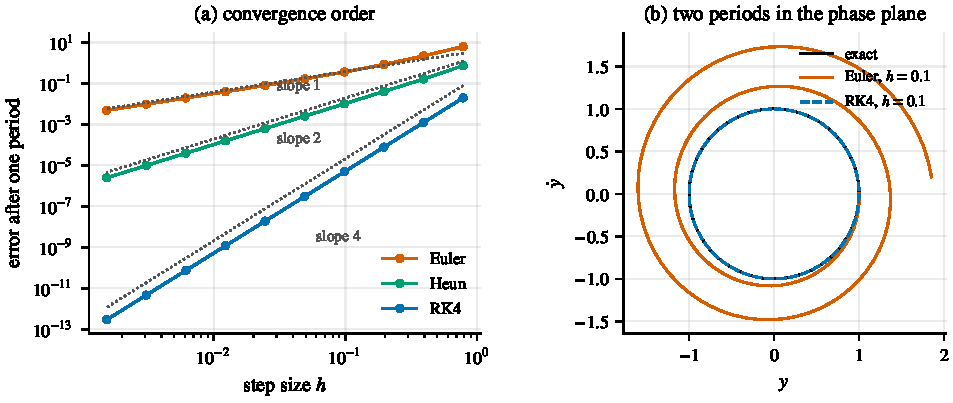
\includegraphics[width=\textwidth]{fig_ode_methods.pdf}
  \caption{Integrating the harmonic oscillator $\ddot y = -y$. (a) Global error after one period versus step size: slopes 1, 2 and 4 confirm the
  orders of Euler, Heun and RK4. (b) With $h = 0.1$, Euler's method spirals outward, gaining energy every step, while RK4 stays on the
  circle to plotting accuracy.}
  \label{fig:ode-methods}
\end{figure}

\paragraph{Verifying the order.} If the error behaves as $Ch^p$, then halving the step divides the error by $2^p$, and the order can be
\emph{measured}: $p \approx \log_2\big(e(h)/e(h/2)\big)$. \Cref{fig:ode-methods}(a) shows this for three methods. A convergence-order test of
this kind is one of the most powerful tests of an integrator: an implementation bug almost always destroys the expected order
(Milestone 4).

\paragraph{Stability.} Euler's method applied to the decaying equation $\dot x = -\lambda x$ gives $x_{k+1} = (1 - h\lambda)x_k$, which blows up
when $h > 2/\lambda$, although the true solution decays. Stiff systems, with very fast decaying modes, need tiny steps or implicit methods.
Applied to an oscillator, Euler's method multiplies the amplitude by $\sqrt{1 + h^2\omega^2} > 1$ per step and spirals outward
(\cref{fig:ode-methods}b). Inertial navigation is not stiff, but this effect is the reason a naive attitude integrator slowly inflates the
norm of its rotation matrix, as we now see.

\subsection{Integrating on a curved space}
\label{sec:lie-euler}

Apply Euler's method to the attitude kinematics $\dot R = R\sx{\omega}$: $R_{k+1} = R_k + hR_k\sx{\omega} = R_k(I + h\sx{\omega})$. The result
is not a rotation matrix:
\begin{equation}
  (I + h\sx{\omega})\T(I + h\sx{\omega}) = I - h^2\sx{\omega}^2 \neq I,
\end{equation}
so every step stretches vectors perpendicular to $\omega$ by a factor of about $1 + \tfrac12h^2\|\omega\|^2$, and the matrix drifts off the set of
rotations. The remedy is to integrate in a way that respects the structure of the space. For constant $\omega$ over the step, the exact
solution is $R_k\exp(h\sx{\omega})$ (\cref{thm:lti-solution}), so the \emph{Lie--Euler} method
\begin{equation}
  R_{k+1} = R_k\exp(h\sx{\omega_k})
\end{equation}
stays exactly on the set of rotations (\cref{prop:exp-skew}) and is first order in general, exact when $\omega$ is constant. Higher-order
generalizations (Runge--Kutta--Munthe-Kaas methods) apply Runge--Kutta to a vector-space parameterization of the increment. Every attitude
update in these notes is multiplicative in this sense (AGENTS.md F1).

% ==============================================================================
\section{Numerical differentiation}
\label{sec:numdiff}

Analytic Jacobians are derived by hand and verified numerically (AGENTS.md E6). Numerical differentiation is easy to write and easy to
get subtly wrong, because it is a subtraction of nearly equal numbers.

\paragraph{Forward differences.} By Taylor's theorem,
\begin{equation}
  \frac{f(x + h) - f(x)}{h} = f'(x) + \frac h2f''(\xi),
\end{equation}
so the \emph{truncation error} is about $\frac h2|f''|$. But $f(x + h)$ and $f(x)$ are each computed with a rounding error of about $u|f|$, and
their difference is divided by $h$, which adds a \emph{rounding error} of about $2u|f|/h$. The total $\frac h2|f''| + \frac{2u|f|}{h}$ is minimized at
$h^\star = 2\sqrt{u|f|/|f''|} \approx 10^{-8}$ for quantities of order one, with a total error of about $10^{-8}$.

\paragraph{Central differences.} Expanding both $f(x \pm h)$,
\begin{equation}
  \frac{f(x + h) - f(x - h)}{2h} = f'(x) + \frac{h^2}{6}f'''(\xi),
\end{equation}
because the even-order terms cancel. The total error $\frac{h^2}6|f'''| + \frac{u|f|}{h}$ is minimized at
\begin{equation}
  h^\star = \left(\frac{3\,u\,|f|}{|f'''|}\right)^{1/3} \approx 10^{-5}\text{ to }10^{-6},
\end{equation}
with a total error of order $u^{2/3} \approx 10^{-11}$.

\begin{figure}[t]
  \centering
  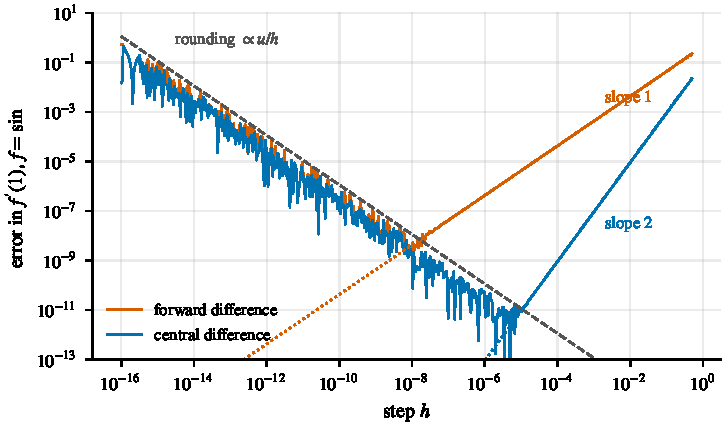
\includegraphics[width=0.85\textwidth]{fig_fd_error.pdf}
  \caption{Error of finite-difference derivatives of $\sin x$ at $x = 1$ versus step size. To the right of the optimum, truncation error
  dominates (slopes 1 and 2); to the left, rounding error grows like $u/h$. Central differences reach about $10^{-11}$; forward differences
  only about $10^{-8}$.}
  \label{fig:fd-error}
\end{figure}

\Cref{fig:fd-error} shows both error regimes. This is why the Jacobian tests of the project use central differences with $h \approx 10^{-6}$
and tolerances of about $10^{-6}$ to $10^{-8}$ relative to the size of the entries. A tolerance tighter than the achievable accuracy makes a
correct implementation fail; a much looser one lets a wrong implementation pass.

\paragraph{Jacobians.} For $f: \R^n \to \R^m$, column $j$ of the numerical Jacobian is
$\big(f(x + he_j) - f(x - he_j)\big)/2h$, costing $2n$ evaluations of $f$. On manifolds the perturbation and the difference are replaced by
$\bplus$ and $\bminus$ (\cref{ch:lie}); nothing else changes.

\begin{aside}[the complex-step derivative]
If $f$ is analytic and can be evaluated with complex arguments, $f'(x) = \operatorname{Im}f(x + ih)/h + O(h^2)$, with no subtraction at all.
With $h = 10^{-20}$ the result is exact to machine precision. The technique requires that every operation in $f$ be implemented for complex
numbers and avoid non-analytic functions (absolute values, comparisons), which rules it out for most estimator code. It is a superb way to
generate reference Jacobians in Python, though.
\end{aside}

\begin{takeaways}
\begin{itemize}
  \item The Jacobian is the matrix of the best linear approximation; the chain rule multiplies Jacobians in composition order.
  \item Taylor's theorem bounds approximation errors. ``First order'' means an error of $O(\|\delta\|^2)$.
  \item $\dd(A\inv) = -A\inv\dd A\,A\inv$ and $\dd\log\det A = \tr(A\inv\dd A)$.
  \item $\dot x = Ax + Bu$ is solved by $e^{At}$ plus a convolution of the inputs; time-varying systems use the state transition matrix,
        which is \emph{not} the exponential of the integrated system matrix unless the matrices commute.
  \item A method of order $p$ has global error $O(h^p)$; halving the step should divide the error by $2^p$. Measure it.
  \item Euler's method leaves the set of rotations; multiplicative updates $R\exp(h\sx{\omega})$ do not.
  \item Central differences with $h \approx 10^{-6}$ reach about $10^{-11}$ accuracy; forward differences only about $10^{-8}$.
\end{itemize}
\end{takeaways}

\begin{exercises}
  \item Compute the Jacobian of $f(x, y) = (x^2y, \sin(xy), e^x)$ and verify it with central differences.
  \item Use Taylor's theorem to bound the error of $\cos h \approx 1 - h^2/2$ for $|h| \le 0.1$.
  \item Show that $\nabla_x\|Ax - b\|^2 = 2A\T(Ax - b)$ and $\nabla_x^2\|Ax - b\|^2 = 2A\T A$.
  \item Solve $\dot x = -2x + 1$, $x(0) = 3$, and check the solution by substitution.
  \item For $A = \begin{bmatrix}0 & 1\\ -1 & 0\end{bmatrix}$, compute $e^{At}$ and interpret the solution of $\dot x = Ax$.
  \item Find the state transition matrix of $\dot x = \begin{bmatrix}0 & t\\0 & 0\end{bmatrix}x$. Do the matrices $A(t)$ commute?
  \item Construct two angular velocity profiles with the same integral $\int\omega\,\dd t$ that produce different final rotations.
  \item Implement Euler, Heun and RK4 for the harmonic oscillator and reproduce \cref{fig:ode-methods}(a).
  \item Show that one Euler step on $\dot R = R\sx{\omega}$ increases $\det R$ by a factor $1 + h^2\|\omega\|^2$, to leading order.
  \item Reproduce \cref{fig:fd-error} and compare the observed optimal step sizes with the formulas of \cref{sec:numdiff}.
\end{exercises}
% Solutions to the exercises of Chapter 4.
\begin{solutions}
  \item Differentiating each component with respect to $x$ and $y$,
        \[
          \frac{\partial f}{\partial(x, y)} = \begin{bmatrix} 2xy & x^2 \\ y\cos(xy) & x\cos(xy) \\ e^x & 0 \end{bmatrix}.
        \]
        At $(x, y) = (0.7, -1.3)$ this is $\begin{bmatrix}-1.82 & 0.49\\ -0.798 & 0.430\\ 2.014 & 0\end{bmatrix}$, and the central-difference Jacobian
        with $h = 10^{-6}$, column $j$ being $\big(f(x + he_j) - f(x - he_j)\big)/2h$, agrees to $10^{-10}$, the accuracy predicted in
        \cref{sec:numdiff}.

  \item The cubic Taylor term of $\cos$ at $0$ vanishes, so $1 - h^2/2$ is also the degree-3 Taylor polynomial, and \cref{thm:taylor} with $n = 3$
        gives the remainder $\cos(\xi)\,h^4/4!$. Hence $|\cos h - (1 - h^2/2)| \le h^4/24 \le 4.2\times10^{-6}$ for $|h| \le 0.1$. The bound is tight:
        at $h = 0.1$ the actual error is $4.165\times10^{-6}$. Using $n = 2$ instead would give the much weaker bound $|h|^3/6 \approx 1.7\times10^{-4}$;
        knowing which terms vanish pays off.

  \item Expand $f(x) = \|Ax - b\|^2 = x\T A\T Ax - 2b\T Ax + b\T b$. The quadratic-form rule with the symmetric matrix $A\T A$ gives
        $\nabla(x\T A\T Ax) = 2A\T Ax$, and $\nabla(b\T Ax) = A\T b$, so
        \[
          \nabla_xf = 2A\T Ax - 2A\T b = 2A\T(Ax - b), \qquad \nabla^2_xf = \frac{\partial}{\partial x}\big(2A\T Ax - 2A\T b\big) = 2A\T A .
        \]
        Setting the gradient to zero gives the normal equations; the Hessian $2A\T A \succeq 0$ shows that any such point is a minimum.

  \item With $a = -2$ and $b = 1$ the integrating-factor formula gives
        \[
          x(t) = 3e^{-2t} + \int_0^te^{-2(t-s)}\,\dd s = 3e^{-2t} + \tfrac12\big(1 - e^{-2t}\big) = \tfrac12 + \tfrac52e^{-2t}.
        \]
        Check: $\dot x = -5e^{-2t}$ and $-2x + 1 = -1 - 5e^{-2t} + 1 = -5e^{-2t}$; $x(0) = \tfrac12 + \tfrac52 = 3$. The solution decays from 3 to the
        equilibrium $\tfrac12$ with time constant $\tfrac12$.

  \item $A^2 = -I$, so as in the solution of Exercise 3.7 the series splits into the cosine and sine series:
        \[
          e^{At} = \cos t\,I + \sin t\,A = \begin{bmatrix}\cos t & \sin t\\ -\sin t & \cos t\end{bmatrix}.
        \]
        This is a rotation by $-t$. The system is $\dot x_1 = x_2$, $\dot x_2 = -x_1$, the harmonic oscillator $\ddot x_1 = -x_1$ with
        $x_1 = \text{position}$ and $x_2 = \text{velocity}$. Its solutions move clockwise around circles at unit angular rate; $\|x\|^2$, the energy, is
        conserved. (Euler's method fails to conserve it, \cref{fig:ode-methods}b.)

  \item The second equation gives $x_2(t) = x_2(s)$, and then $\dot x_1 = t\,x_2(s)$ integrates to $x_1(t) = x_1(s) + \tfrac12(t^2 - s^2)x_2(s)$, so
        \[
          \Phi(t, s) = \begin{bmatrix}1 & \tfrac12(t^2 - s^2)\\ 0 & 1\end{bmatrix}.
        \]
        The matrices do commute: $A(t)A(s) = \begin{bmatrix}0 & t\\0 & 0\end{bmatrix}\begin{bmatrix}0 & s\\0 & 0\end{bmatrix} = 0 = A(s)A(t)$.
        Accordingly property 4 of \cref{prop:stm} applies: $\int_s^tA = \begin{bmatrix}0 & \frac12(t^2 - s^2)\\0 & 0\end{bmatrix}$ is nilpotent and its
        exponential is exactly $\Phi(t, s)$.

  \item Profile A: rotate about $x$ at $\pi/2$~rad/s for one second, then about $y$ at $\pi/2$~rad/s for one second. Profile B: the same two
        segments in the opposite order. Both have $\int\omega\,\dd t = (\pi/2, \pi/2, 0)$. With body rates, $R = R(0)\exp(\cdot)\exp(\cdot)$, so the final
        rotations are
        \[
          R_A = R_x(90^\circ)R_y(90^\circ) = \begin{bmatrix}0 & 0 & 1\\ 1 & 0 & 0\\ 0 & 1 & 0\end{bmatrix}, \qquad
          R_B = R_y(90^\circ)R_x(90^\circ) = \begin{bmatrix}0 & 1 & 0\\ 0 & 0 & -1\\ -1 & 0 & 0\end{bmatrix},
        \]
        both $120^\circ$ rotations but about different axes, $120^\circ$ apart from each other. Neither equals $\exp(\sx{(\pi/2, \pi/2, 0)})$, a
        $127^\circ$ rotation about $(1, 1, 0)/\sqrt2$. The integral of $\omega$ does not determine the rotation; the order of the rotations does.

  \item The implementation follows the formulas of \cref{sec:numint}, with $f(y) = (y_2, -y_1)$, $y_0 = (1, 0)$, and $N$ steps of $h = 2\pi/N$ over one
        period:
\begin{lstlisting}[style=py]
def step(method, y, h):
    f = lambda y: np.array([y[1], -y[0]])
    if method == "Euler": return y + h * f(y)
    if method == "Heun":
        k1 = f(y); k2 = f(y + h * k1); return y + h / 2 * (k1 + k2)
    k1 = f(y); k2 = f(y + h/2 * k1); k3 = f(y + h/2 * k2); k4 = f(y + h * k3)
    return y + h / 6 * (k1 + 2 * k2 + 2 * k3 + k4)
\end{lstlisting}
        The final errors $\|y_N - y_0\|$ for $N = 32, 64, 128, 256$ are $0.84, 0.36, 0.17, 0.080$ (Euler), $4.1\times10^{-2}, 1.0\times10^{-2},
        2.5\times10^{-3}, 6.3\times10^{-4}$ (Heun) and $7.8\times10^{-5}, 4.9\times10^{-6}, 3.0\times10^{-7}, 1.9\times10^{-8}$ (RK4). The ratios between
        successive errors give measured orders $\log_2(e_h/e_{h/2}) \approx 1.1$, $2.0$ and $4.0$. Euler approaches order 1 only slowly because its
        errors are still large: at $N = 32$ the amplitude has already grown by $\big(1 + (2\pi/32)^2\big)^{16} \approx 1.8$.

  \item One Euler step is $R_{k+1} = R_k(I + h\sx{\omega})$, so $\det R_{k+1} = \det R_k\,\det(I + h\sx{\omega})$. The eigenvalues of $\sx{\omega}$ are $0$
        and $\pm i\|\omega\|$ (Exercise 2.7), so those of $I + h\sx{\omega}$ are $1$ and $1 \pm ih\|\omega\|$, and
        \[
          \det(I + h\sx{\omega}) = 1\cdot(1 + ih\|\omega\|)(1 - ih\|\omega\|) = 1 + h^2\|\omega\|^2 .
        \]
        The factor is in fact exact, not only leading order. After $n$ steps $\det R = (1 + h^2\|\omega\|^2)^n \approx e^{nh^2\|\omega\|^2}$: at 200~Hz and
        1~rad/s this is $e^{2.5\times10^{-5}\,n}$, a 2.5\% inflation per thousand steps. The Lie--Euler update $R_k\exp(h\sx{\omega})$ keeps $\det R = 1$ exactly.

  \item Evaluating the two formulas of \cref{sec:numdiff} on a log-spaced grid of $h$ for $f = \sin$ at $x = 1$ reproduces the figure. The theory
        predicts, with $u = 2^{-53}$, $|f| = \sin1 = 0.84$, $|f''| = 0.84$, $|f'''| = \cos1 = 0.54$:
        \begin{itemize}[leftmargin=1.2em]
          \item forward differences: $h^\star = 2\sqrt{u|f|/|f''|} = 2.1\times10^{-8}$, with error $2\sqrt{u|f||f''|} = 1.8\times10^{-8}$;
          \item central differences: $h^\star = (3u|f|/|f'''|)^{1/3} = 8.0\times10^{-6}$, with error $1.7\times10^{-11}$.
        \end{itemize}
        The observed minima (taking the median error in a small window of $h$, since the rounding part is erratic) lie at $h \approx 10^{-8}$ and
        $5\times10^{-6}$, with errors of about $3\times10^{-9}$ and $3\times10^{-12}$. The optimal steps agree with the formulas to within a factor of
        two, and the observed errors are a few times smaller than the predicted ones, because the formulas add worst-case rounding errors while
        the actual rounding errors of $f(x + h)$ and $f(x - h)$ are partly random and partly cancel.
\end{solutions}


\chapter{Probability and Random Vectors}
\label{ch:prob}

\begin{objectives}
\begin{itemize}
  \item Build probability from its axioms: conditional probability, independence and Bayes' rule.
  \item Work with random variables and random vectors: densities, expectations, covariances and changes of variables.
  \item Derive the Gaussian distribution and its key properties: affine maps, marginals, conditionals and the fusion of estimates.
  \item Understand the law of large numbers, the central limit theorem and Monte Carlo methods.
  \item Derive the $\chi^2$ distribution and use it for hypothesis tests, the basis of gating and consistency checks.
  \item Understand how nonlinear functions distort distributions, and what linearization keeps and loses.
\end{itemize}
\end{objectives}

A filter does not merely estimate the state; it maintains a probability distribution over it. The estimate is the center of
that distribution, and the covariance describes its spread. This chapter develops the probability theory that gives these words a
precise meaning.

% ==============================================================================
\section{Probability}

\subsection{Events and the axioms}

A random experiment has a set $\Omega$ of possible outcomes, the \term{sample space}. An \term{event} is a subset of outcomes, and a
\term{probability} assigns to each event $A$ a number $P(A)$ obeying three axioms (Kolmogorov):
\begin{enumerate}
  \item $P(A) \ge 0$ for every event;
  \item $P(\Omega) = 1$;
  \item if $A_1, A_2, \dots$ are mutually exclusive (pairwise disjoint), $P(A_1\cup A_2\cup\cdots) = \sum_iP(A_i)$.
\end{enumerate}
Everything else follows: $P(\text{not }A) = 1 - P(A)$, $P(A\cup B) = P(A) + P(B) - P(A\cap B)$, and so on. Probability can be read as a
long-run frequency (the fraction of repetitions in which $A$ occurs) or as a degree of belief; the mathematics is the same, and filters
use both readings.

\subsection{Conditional probability and independence}

\begin{definition}[Conditional probability]
For $P(B) > 0$, the probability of $A$ given $B$ is $P(A\mid B) = P(A\cap B)/P(B)$.
\end{definition}

Conditioning restricts attention to the outcomes in which $B$ happened and renormalizes. Two events are \term{independent} if
$P(A\cap B) = P(A)P(B)$, equivalently $P(A\mid B) = P(A)$: knowing that $B$ occurred tells nothing about $A$.

\begin{proposition}[Law of total probability and Bayes' rule]
\index{Bayes' rule}
If $B_1, \dots, B_n$ are mutually exclusive and cover $\Omega$, then $P(A) = \sum_iP(A\mid B_i)P(B_i)$, and
\begin{equation}
  P(B_i\mid A) = \frac{P(A\mid B_i)\,P(B_i)}{\sum_jP(A\mid B_j)\,P(B_j)} .
\end{equation}
\end{proposition}
\begin{proof}
$A$ is the disjoint union of the $A\cap B_i$, and $P(A\cap B_i) = P(A\mid B_i)P(B_i)$. Bayes' rule is the definition of conditional
probability applied twice: $P(B_i\mid A)P(A) = P(A\cap B_i) = P(A\mid B_i)P(B_i)$.
\end{proof}

Bayes' rule turns the probability of an observation given a hypothesis (which a sensor model provides) into the probability of the
hypothesis given the observation (which we want).

\begin{worked}[how informative is a passed test?]
Suppose 10\% of the feature tracks reaching an outlier test are wrong. The test rejects 90\% of wrong tracks, and (being a 95\% gate)
also rejects 5\% of correct ones. A track passes. What is the probability that it is wrong? With $W$ = ``wrong'' and $A$ = ``passes'':
$P(A\mid W) = 0.1$, $P(W) = 0.1$, $P(A\mid\text{correct}) = 0.95$, $P(\text{correct}) = 0.9$. Bayes' rule gives
\begin{equation*}
  P(W\mid A) = \frac{0.1\times0.1}{0.1\times0.1 + 0.95\times0.9} = \frac{0.01}{0.865} \approx 1.2\% .
\end{equation*}
The test reduces the outlier fraction from 10\% to about 1\%: very useful, but not perfect, which is why the estimator adds further
checks downstream.
\end{worked}

% ==============================================================================
\section{Random variables}

\subsection{Distributions, densities and expectations}

A \term{random variable} $X$ is a numerical quantity determined by the outcome of an experiment. Its \emph{cumulative distribution
function} is $F(x) = P(X \le x)$. A discrete random variable takes countably many values with probabilities $p(x) = P(X = x)$; a continuous
one has a \term{probability density function} (pdf) $p(x) \ge 0$ with
\begin{equation}
  P(a \le X \le b) = \int_a^bp(x)\,\dd x, \qquad \int_{-\infty}^\infty p(x)\,\dd x = 1 .
\end{equation}
A density is not a probability: $p(x)\,\dd x$ is the probability of falling in a small interval of width $\dd x$ around $x$, and a density
can exceed one.

\begin{definition}[Expectation and variance]
The \term{expectation} (mean) of $X$ is $\E[X] = \int x\,p(x)\,\dd x$ (a sum for discrete variables). The expectation of a function of $X$ is
$\E[g(X)] = \int g(x)p(x)\,\dd x$. The \term{variance} is $\Var(X) = \E[(X - \E X)^2] = \E[X^2] - (\E X)^2$, and its square root is the
\term{standard deviation} $\sigma$.
\end{definition}

Expectation is linear: $\E[aX + bY + c] = a\E[X] + b\E[Y] + c$ for any random variables, dependent or not. Variance scales quadratically and
ignores shifts: $\Var(aX + c) = a^2\Var(X)$. The standard deviation has the units of $X$ and measures its typical spread.

\begin{example}[Uniform distribution]
$X$ uniform on $[a, b]$ has $p(x) = 1/(b - a)$ there, mean $(a + b)/2$ and variance $(b - a)^2/12$. Rounding a reading to a resolution
$\Delta$ produces an error that is approximately uniform on $[-\Delta/2, \Delta/2]$, with standard deviation $\Delta/\sqrt{12}$: the
quantization noise of a sensor.
\end{example}

\subsection{The Gaussian distribution}

\begin{definition}[Gaussian distribution]
\index{Gaussian distribution}
$X \sim \N(\mu, \sigma^2)$ has density
\begin{equation}
  p(x) = \frac{1}{\sqrt{2\pi}\,\sigma}\exp\!\Big(-\frac{(x - \mu)^2}{2\sigma^2}\Big).
\end{equation}
The \emph{standard normal} distribution is $\N(0, 1)$.
\end{definition}

\begin{proposition}[Normalization]
$\int_{-\infty}^\infty e^{-x^2/2}\,\dd x = \sqrt{2\pi}$.
\end{proposition}
\begin{proof}
Let $I$ be the integral. Then $I^2 = \iint e^{-(x^2 + y^2)/2}\,\dd x\,\dd y$. In polar coordinates, with area element $r\,\dd r\,\dd\theta$,
$I^2 = \int_0^{2\pi}\!\int_0^\infty e^{-r^2/2}r\,\dd r\,\dd\theta = 2\pi\big[-e^{-r^2/2}\big]_0^\infty = 2\pi$.
\end{proof}

Substituting $x \to (x - \mu)/\sigma$ shows that the general density integrates to one, and similar integrals (using symmetry and
integration by parts) give $\E[X] = \mu$ and $\Var(X) = \sigma^2$. If $X \sim \N(\mu, \sigma^2)$ then $(X - \mu)/\sigma \sim \N(0, 1)$, and the
probabilities of falling within one, two and three standard deviations of the mean are $68.27\%$, $95.45\%$ and $99.73\%$. A Gaussian is
completely determined by its mean and variance, and is closed under the operations a linear filter performs, which is why Kalman
filters can work with means and covariances alone.

% ==============================================================================
\section{Several random variables}

\subsection{Joint, marginal and conditional densities}

Two random variables $X, Y$ have a \emph{joint density} $p(x, y)$, with $P((X, Y) \in A) = \iint_Ap(x, y)\,\dd x\,\dd y$. From it:
\begin{align}
  \text{marginal:}&\quad p(x) = \int p(x, y)\,\dd y, \\
  \text{conditional:}&\quad p(x\mid y) = \frac{p(x, y)}{p(y)}, \\
  \text{Bayes' rule:}&\quad p(x\mid y) = \frac{p(y\mid x)\,p(x)}{p(y)} = \frac{p(y\mid x)\,p(x)}{\int p(y\mid x')p(x')\,\dd x'} .
\end{align}
$X$ and $Y$ are independent if $p(x, y) = p(x)p(y)$. In estimation, $x$ is the unknown state and $y$ the measurement: $p(y\mid x)$ is the
sensor model (the \emph{likelihood}), $p(x)$ is the \emph{prior}, and $p(x\mid y)$ the \emph{posterior}.

\subsection{Covariance and correlation}

The \term{covariance} $\Cov(X, Y) = \E[(X - \E X)(Y - \E Y)]$ measures how two variables vary together, and the \term{correlation
coefficient} $\rho = \Cov(X, Y)/(\sigma_X\sigma_Y) \in [-1, 1]$ normalizes it (the bound is the Cauchy--Schwarz inequality). Independent
variables have zero covariance, and then $\Var(X + Y) = \Var(X) + \Var(Y)$: variances of independent errors add.

The converse fails: zero correlation does not imply independence. If $X \sim \N(0, 1)$ and $Y = X^2$, then $\Cov(X, Y) = \E[X^3] = 0$, yet $Y$
is a function of $X$. Correlation measures only \emph{linear} dependence. (For jointly Gaussian variables the converse does hold, as shown
below.)

% ==============================================================================
\section{Random vectors}

\subsection{Mean and covariance}

For a random vector $x \in \R^n$ with density $p(x)$, the mean and \term{covariance matrix} are
\begin{equation}
  \mu = \E[x], \qquad \Sigma = \Cov(x) = \E\big[(x - \mu)(x - \mu)\T\big] = \E[xx\T] - \mu\mu\T .
\end{equation}
The diagonal of $\Sigma$ holds the variances $\sigma_i^2$ and its off-diagonal entries the covariances. $\Sigma$ is symmetric and positive
semi-definite: for any fixed $a$, $a\T\Sigma a = \E\big[(a\T(x - \mu))^2\big] \ge 0$. The \emph{cross-covariance} of two random vectors is
$\Sigma_{xy} = \E[(x - \mu_x)(y - \mu_y)\T]$, and $\Sigma_{yx} = \Sigma_{xy}\T$.

\begin{proposition}[Affine transformations]
\label{prop:affine}
If $y = Ax + b$ then $\E[y] = A\mu + b$ and $\Cov(y) = A\Sigma A\T$. If $x$ and $w$ are uncorrelated, $\Cov(Ax + Bw) = A\Sigma_xA\T + B\Sigma_wB\T$.
\end{proposition}
\begin{proof}
Linearity of expectation gives the mean. Then $\Cov(y) = \E[A(x - \mu)(x - \mu)\T A\T] = A\Sigma A\T$. With uncorrelated $x$ and $w$, the cross terms
$A\Sigma_{xw}B\T$ vanish.
\end{proof}

This one proposition is the covariance propagation of the Kalman filter ($P \leftarrow \Phi P \Phi\T + Q$), the covariance of a stacked
measurement, and the augmentation formula of stochastic cloning ($P \leftarrow JPJ\T$).

\begin{proposition}[Expected value of a quadratic form]
\label{prop:quadratic-expectation}
For any matrix $A$, $\E[x\T Ax] = \tr(A\Sigma) + \mu\T A\mu$. In particular, if $\mu = 0$ then $\E[x\T\Sigma\inv x] = \tr(I_n) = n$.
\end{proposition}
\begin{proof}
$x\T Ax = \tr(Axx\T)$, and expectation commutes with the trace: $\E[x\T Ax] = \tr(A\,\E[xx\T]) = \tr(A(\Sigma + \mu\mu\T))$.
\end{proof}

The special case is the reason a consistent filter's normalized estimation error squared averages to the dimension of the state
(\cref{ch:consistency}).

\subsection{Changing variables}

\begin{proposition}[Change of variables]
\label{prop:change-of-variables}
If $y = g(x)$ with $g$ invertible and differentiable, the densities are related by
$p_y(y) = p_x\big(g\inv(y)\big)\,\big|\det\frac{\partial g\inv}{\partial y}\big|$.
\end{proposition}

In one dimension this follows from equating probabilities of corresponding small intervals, $p_y(y)\,|\dd y| = p_x(x)\,|\dd x|$; in several
dimensions the determinant measures how $g\inv$ stretches volumes (\cref{sec:determinants}). For an invertible linear map $y = Ax$ the factor
is the constant $1/|\det A|$.

% ==============================================================================
\section{The multivariate Gaussian}

\subsection{Definition}

\begin{definition}[Multivariate Gaussian]
\index{Gaussian distribution!multivariate}
A random vector $x \in \R^n$ is Gaussian, $x \sim \N(\mu, \Sigma)$, if it can be written as $x = \mu + Ls$ where $s$ has independent standard
normal components and $LL\T = \Sigma$. If $\Sigma \succ 0$ its density is
\begin{equation}
  p(x) = \frac{1}{\sqrt{(2\pi)^n \det\Sigma}}\exp\!\Big( -\tfrac12 (x - \mu)\T \Sigma\inv (x - \mu) \Big).
  \label{eq:gaussian-pdf}
\end{equation}
The quantity $d_M^2(x) = (x - \mu)\T\Sigma\inv(x - \mu)$ is the squared \term{Mahalanobis distance} of $x$ from the mean.
\end{definition}

\begin{proof}[Derivation of the density]
The density of $s$ is the product of $n$ standard normal densities, $(2\pi)^{-n/2}\exp(-\tfrac12s\T s)$. By \cref{prop:change-of-variables} with
$s = L\inv(x - \mu)$, $p(x) = (2\pi)^{-n/2}\exp\big(-\tfrac12(x - \mu)\T L\mT L\inv(x - \mu)\big)/|\det L|$. Since $L\mT L\inv = (LL\T)\inv = \Sigma\inv$ and
$|\det L| = \sqrt{\det\Sigma}$, this is \eqref{eq:gaussian-pdf}.
\end{proof}

By \cref{prop:affine}, the mean of $x$ is $\mu$ and its covariance is $L\,\E[ss\T]L\T = \Sigma$. The definition also handles singular
covariances (with $L$ not invertible), which arise naturally in stochastic cloning (\cref{ch:cloning}).

\begin{figure}[t]
  \centering
  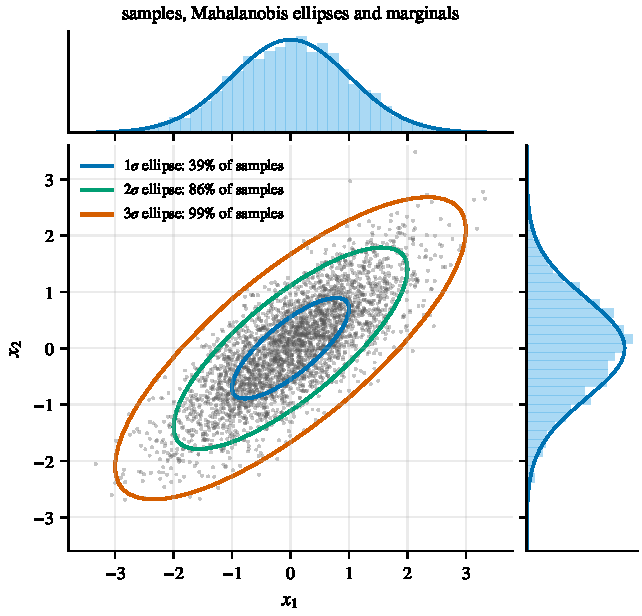
\includegraphics[width=0.92\textwidth]{fig_gauss2d.pdf}
  \caption{Samples of a correlated 2D Gaussian with the $1\sigma$, $2\sigma$ and $3\sigma$ Mahalanobis ellipses, and the two marginal densities.
  The ellipses are aligned with the eigenvectors of $\Sigma$. In two dimensions they contain 39\%, 86\% and 99\% of the probability, not
  the familiar 68--95--99.7\% of one dimension.}
  \label{fig:gauss2d}
\end{figure}

\paragraph{Geometry.} The density is constant on the ellipsoids $d_M^2(x) = c$, whose axes point along the eigenvectors of $\Sigma$ with lengths
proportional to the square roots of its eigenvalues (\cref{fig:ellipse,fig:gauss2d}). The Mahalanobis distance measures distance in units of
standard deviations along each principal axis, which makes it the natural way to ask whether a vector is ``far'' from a distribution.

\paragraph{Sampling.} To draw from $\N(\mu, \Sigma)$, factor $\Sigma = LL\T$ (Cholesky), draw $s \sim \N(0, I)$, and return $\mu + Ls$. Monte Carlo tests
of covariance propagation (Milestone 5) use exactly this.

\paragraph{Closure.} Affine maps of Gaussian vectors are Gaussian (directly from the definition). Marginals, conditionals and products of
Gaussian densities are Gaussian (next section). Hence a Gaussian belief propagated through a linear system with Gaussian noise remains
exactly Gaussian, and the Kalman filter is exact in that case. For jointly Gaussian vectors, uncorrelated implies independent: if the
covariance is block diagonal, the density factors.

\paragraph{Information form.} A Gaussian can equally be parameterized by the \term{information matrix} $\Lambda = \Sigma\inv$ and the
\emph{information vector} $\eta = \Sigma\inv\mu$. Then $-\log p(x) = \tfrac12 x\T\Lambda x - \eta\T x + \text{const}$. The information form is natural
for combining independent pieces of evidence, since their information adds, and it is the form in which optimization-based estimators work.

\subsection{Marginals and conditionals}

Partition a jointly Gaussian vector as
\begin{equation}
  \begin{bmatrix} a \\ b \end{bmatrix} \sim
  \N\!\left( \begin{bmatrix} \mu_a \\ \mu_b \end{bmatrix},
  \begin{bmatrix} \Sigma_{aa} & \Sigma_{ab} \\ \Sigma_{ba} & \Sigma_{bb} \end{bmatrix} \right),
  \qquad
  \Lambda = \Sigma\inv = \begin{bmatrix} \Lambda_{aa} & \Lambda_{ab} \\ \Lambda_{ba} & \Lambda_{bb} \end{bmatrix}.
\end{equation}

\begin{theorem}[Gaussian marginalization and conditioning]
\label{thm:gauss-cond}
\index{marginalization}\index{conditioning}
\begin{enumerate}
  \item The marginal of $a$ is $\N(\mu_a, \Sigma_{aa})$.
  \item The conditional of $a$ given $b$ is $\N(\mu_{a|b}, \Sigma_{a|b})$ with
  \begin{equation}
    \mu_{a|b} = \mu_a + \Sigma_{ab}\Sigma_{bb}\inv (b - \mu_b), \qquad
    \Sigma_{a|b} = \Sigma_{aa} - \Sigma_{ab}\Sigma_{bb}\inv\Sigma_{ba}.
    \label{eq:gauss-cond}
  \end{equation}
\end{enumerate}
\end{theorem}
\begin{proof}
The marginal follows from \cref{prop:affine} with the selection matrix $A = [I\ \ 0]$. For the conditional, define
$\tilde a = a - \Sigma_{ab}\Sigma_{bb}\inv b$. Then $\Cov(\tilde a, b) = \Sigma_{ab} - \Sigma_{ab}\Sigma_{bb}\inv\Sigma_{bb} = 0$, so $\tilde a$ and $b$ are uncorrelated,
and being jointly Gaussian they are independent. By \cref{prop:affine},
$\tilde a \sim \N(\mu_a - \Sigma_{ab}\Sigma_{bb}\inv\mu_b,\ \Sigma_{aa} - \Sigma_{ab}\Sigma_{bb}\inv\Sigma_{ba})$. Conditioning on $b$ leaves the distribution of
$\tilde a$ unchanged (independence), and $a = \tilde a + \Sigma_{ab}\Sigma_{bb}\inv b$, which gives \eqref{eq:gauss-cond}.
\end{proof}

The conditional mean moves away from $\mu_a$ in proportion to how far $b$ is from its mean, by the ``regression'' matrix $\Sigma_{ab}\Sigma_{bb}\inv$,
and the conditional covariance shrinks by a positive semi-definite amount. It does not depend on the observed value of $b$, only on the
fact that it was observed. The conditional covariance is the Schur complement $\Sigma/\Sigma_{bb}$; applying \cref{prop:block-inverse} to $\Sigma$
shows that $\Lambda_{aa} = \Sigma_{a|b}\inv$ and that the marginal information matrix is a Schur complement of $\Lambda$. The two parameterizations
therefore swap the roles of the two operations:

\begin{center}\small
\begin{tabular}{@{}lll@{}}
\toprule
 & covariance form $(\mu, \Sigma)$ & information form $(\eta, \Lambda)$ \\
\midrule
marginalize out $b$ & $\Sigma_{aa}$ \hfill(\textbf{delete rows/columns}) & $\Lambda_{aa} - \Lambda_{ab}\Lambda_{bb}\inv\Lambda_{ba}$ \hfill(Schur compl.) \\
condition on $b$ & $\Sigma_{aa} - \Sigma_{ab}\Sigma_{bb}\inv\Sigma_{ba}$ \hfill(Schur compl.) & $\Lambda_{aa}$ \hfill(\textbf{delete rows/columns}) \\
\bottomrule
\end{tabular}
\end{center}

\begin{keyidea}[marginalization is free in covariance form]
A Kalman filter stores covariances, so discarding a variable (the oldest clone of the MSCKF window) is literally deleting its rows and
columns from $P$. Optimization-based estimators store information matrices, so the same operation requires a Schur complement, which
creates fill-in and the ``marginalization prior'' of sliding-window smoothers (\cref{ch:nlls}).
\end{keyidea}

% ==============================================================================
\section{Fusing information: Bayes' rule for Gaussians}

\subsection{Combining two estimates}

Suppose two independent sensors measure the same scalar $x$, with readings $z_1 = x + n_1$ and $z_2 = x + n_2$ and noise variances $\sigma_1^2$ and
$\sigma_2^2$. With no other knowledge of $x$, the posterior density is proportional to the product of the two likelihoods,
\begin{equation}
  p(x\mid z_1, z_2) \propto \exp\!\Big(-\frac{(x - z_1)^2}{2\sigma_1^2}\Big)\exp\!\Big(-\frac{(x - z_2)^2}{2\sigma_2^2}\Big).
\end{equation}
The exponent is a quadratic in $x$; completing the square shows that the posterior is Gaussian with
\begin{equation}
  \frac{1}{\sigma^2} = \frac1{\sigma_1^2} + \frac1{\sigma_2^2}, \qquad
  \hat x = \sigma^2\Big(\frac{z_1}{\sigma_1^2} + \frac{z_2}{\sigma_2^2}\Big) = z_1 + \frac{\sigma_1^2}{\sigma_1^2 + \sigma_2^2}(z_2 - z_1).
  \label{eq:fusion}
\end{equation}
\emph{Inverse variances (information) add}, and the fused estimate is an information-weighted average. The second form already has the shape
of a Kalman update: start from $z_1$ and correct it by a gain times the discrepancy $z_2 - z_1$, with a gain between 0 and 1 that is large
when the first estimate is poor. The fused variance is smaller than both, so combining independent information always helps.

\subsection{The linear-Gaussian model}

\begin{proposition}[Linear-Gaussian posterior]
\label{prop:map-ls}
If $x \sim \N(\mu, P)$ and $z = Hx + n$ with $n \sim \N(0, R)$ independent of $x$, the posterior $p(x\mid z)$ is Gaussian, and its mean (which is
also its mode) solves the weighted least-squares problem
\begin{equation}
  \hat x = \argmin_x\ \|x - \mu\|^2_{P\inv} + \|z - Hx\|^2_{R\inv},
  \qquad \|e\|^2_{W} := e\T W e .
  \label{eq:map-ls}
\end{equation}
Its covariance is $(P\inv + H\T R\inv H)\inv$.
\end{proposition}
\begin{proof}
By Bayes' rule $p(x\mid z) \propto p(z\mid x)p(x)$, and
$-\log p(x\mid z) = \tfrac12\|x - \mu\|^2_{P\inv} + \tfrac12\|z - Hx\|^2_{R\inv} + \text{const}$. This is a convex quadratic in $x$ whose quadratic term is
$\tfrac12x\T(P\inv + H\T R\inv H)x$, so the posterior is Gaussian with that information matrix, and its mode, which for a Gaussian is the mean,
minimizes the quadratic.
\end{proof}

This is the scalar fusion rule in matrix form: the prior contributes information $P\inv$, the measurement contributes $H\T R\inv H$, and they add.
\Cref{ch:estimation} develops this into the general theory of estimators, and \cref{ch:kf} turns it into the Kalman filter.

% ==============================================================================
\section{Limit theorems and Monte Carlo}

\subsection{The law of large numbers}

Let $X_1, X_2, \dots$ be independent draws from the same distribution, with mean $\mu$ and variance $\sigma^2$, and let
$\bar X_N = \frac1N\sum_{i=1}^NX_i$ be their \term{sample mean}. Then $\E[\bar X_N] = \mu$ and, because variances of independent terms add,
$\Var(\bar X_N) = \sigma^2/N$.

\begin{theorem}[Weak law of large numbers]
\index{law of large numbers}
For every $\epsilon > 0$, $P(|\bar X_N - \mu| > \epsilon) \to 0$ as $N\to\infty$.
\end{theorem}
\begin{proof}
Chebyshev's inequality $P(|Y - \E Y| \ge \epsilon) \le \Var(Y)/\epsilon^2$ (which follows from
$\Var(Y) \ge \E[(Y - \E Y)^2\,\mathbf 1_{|Y - \E Y|\ge\epsilon}] \ge \epsilon^2P(|Y - \E Y|\ge\epsilon)$) applied to $\bar X_N$ gives the bound
$\sigma^2/(N\epsilon^2) \to 0$.
\end{proof}

The law of large numbers justifies \term{Monte Carlo} methods: to estimate an expectation, average many independent samples. The error
shrinks only like $\sigma/\sqrt N$, so each additional digit of accuracy costs a hundred times more samples.

\subsection{The central limit theorem}

\begin{theorem}[Central limit theorem]
\index{central limit theorem}
Under the same assumptions, the distribution of $\sqrt N(\bar X_N - \mu)/\sigma$ converges to $\N(0, 1)$.
\end{theorem}

\begin{figure}[t]
  \centering
  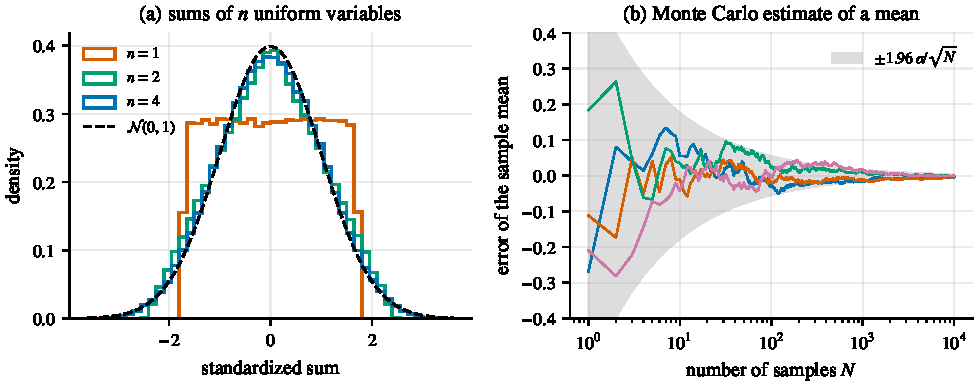
\includegraphics[width=\textwidth]{fig_clt.pdf}
  \caption{(a) The central limit theorem: histograms of the standardized sum of $n$ independent uniform variables approach the standard normal
  density already for $n = 4$. (b) Monte Carlo estimation of a mean: the error of the sample mean shrinks like $1/\sqrt N$ (gray band:
  $\pm1.96\,\sigma/\sqrt N$, the 95\% interval).}
  \label{fig:clt}
\end{figure}

Sums of many small independent effects are approximately Gaussian, whatever the distribution of each effect (\cref{fig:clt}). Electronic
sensor noise is the sum of many microscopic fluctuations, and integrating a noisy signal sums many samples; both are why Gaussian noise
models work well in navigation. They work less well for rare large errors (outliers), which is why estimators also need gating and robust
methods (\cref{ch:updates,ch:nlls}).

% ==============================================================================
\section{The chi-squared distribution}
\label{sec:chi2}

\begin{definition}
\index{chi-squared distribution}
If $s_1, \dots, s_k$ are independent standard normal variables, $\gamma = \sum_{i=1}^k s_i^2$ has the $\chi^2$ distribution with $k$ degrees of freedom,
written $\gamma \sim \chi^2_k$.
\end{definition}

\begin{proposition}[Properties of $\chi^2_k$]
$\E[\gamma] = k$ and $\Var(\gamma) = 2k$. Its density is
\begin{equation}
  p(\gamma) = \frac{\gamma^{k/2 - 1}e^{-\gamma/2}}{2^{k/2}\,\Gamma(k/2)}, \qquad \gamma > 0,
\end{equation}
where $\Gamma$ is the gamma function ($\Gamma(m) = (m - 1)!$ for integers, $\Gamma(\tfrac12) = \sqrt\pi$).
\end{proposition}
\begin{proof}[Proof of the moments and of the case $k = 1$]
For $s \sim \N(0, 1)$, $\E[s^2] = 1$ and $\E[s^4] = 3$ (integration by parts), so $\Var(s^2) = 2$; the moments of the sum follow by additivity
over independent terms. For $k = 1$, $\gamma = s^2$ takes the value $\gamma$ when $s = \pm\sqrt\gamma$, so
$p(\gamma) = 2\cdot\frac{1}{\sqrt{2\pi}}e^{-\gamma/2}\cdot\frac{\dd\sqrt\gamma}{\dd\gamma} = \frac{1}{\sqrt{2\pi\gamma}}e^{-\gamma/2}$, which is the formula with $k = 1$.
The general case follows by convolving densities (or by integrating the Gaussian density over spherical shells).
\end{proof}

\begin{theorem}[Mahalanobis distance of a Gaussian]
\label{thm:mahalanobis-chi2}
If $x \sim \N(\mu, \Sigma)$ in $\R^k$ with $\Sigma \succ 0$, then $(x-\mu)\T\Sigma\inv(x - \mu) \sim \chi^2_k$.
\end{theorem}
\begin{proof}
With $\Sigma = LL\T$, the whitened vector $s = L\inv(x - \mu)$ is $\N(0, I)$ by \cref{prop:affine}, and $(x - \mu)\T\Sigma\inv(x-\mu) = s\T s = \sum_is_i^2$.
\end{proof}

\begin{figure}[t]
  \centering
  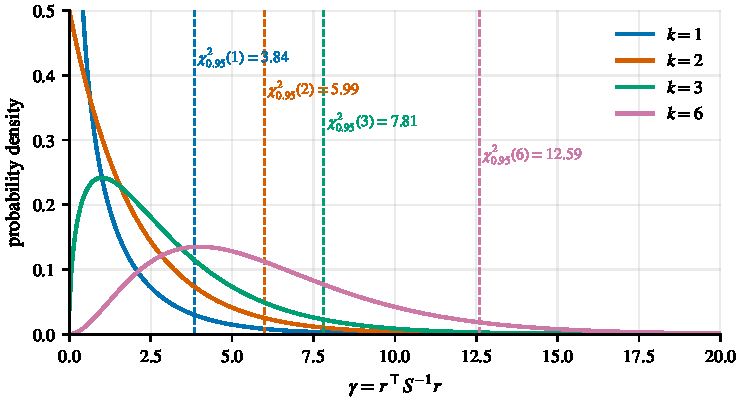
\includegraphics[width=0.84\textwidth]{fig_chi2.pdf}
  \caption{$\chi^2$ densities and their 95\% quantiles. A 2D image measurement whose normalized innovation squared exceeds $5.99$ would occur by
  chance only 5\% of the time if the filter's covariance were correct.}
  \label{fig:chi2}
\end{figure}

The \emph{quantile} $\chi^2_p(k)$ is the value below which a $\chi^2_k$ variable falls with probability $p$ (\cref{fig:chi2}; tables in
\cref{app:tables}). Because independent $\chi^2$ variables add, with their degrees of freedom adding, the sum of $N$ independent squared
Mahalanobis distances of $n$-dimensional Gaussians is $\chi^2_{Nn}$. As $k$ grows, $\chi^2_k$ is approximately $\N(k, 2k)$, so its quantiles approach
$k \pm 1.96\sqrt{2k}$.

% ==============================================================================
\section{Sample statistics and hypothesis tests}

\subsection{Estimating a mean and a variance}

Given independent samples $X_1, \dots, X_N$ of a distribution with unknown mean and variance, the natural estimates are the sample mean
$\bar X$ and the \term{sample variance}
\begin{equation}
  s^2 = \frac{1}{N - 1}\sum_{i=1}^N(X_i - \bar X)^2 .
\end{equation}
The divisor $N - 1$ makes $s^2$ unbiased. Expanding, $\sum_i(X_i - \bar X)^2 = \sum_i(X_i - \mu)^2 - N(\bar X - \mu)^2$, whose expectation is
$N\sigma^2 - N\cdot\sigma^2/N = (N - 1)\sigma^2$: one degree of freedom is used up by estimating the mean. For Gaussian samples one can show
moreover that $(N - 1)s^2/\sigma^2 \sim \chi^2_{N-1}$. This gives exact acceptance intervals for comparing a Monte Carlo sample variance with a
predicted variance, as Milestone 5 requires: the ratio $s^2/\sigma^2$ should lie between $\chi^2_{0.025}(N-1)/(N-1)$ and $\chi^2_{0.975}(N-1)/(N-1)$
95\% of the time (for $N = 500$, between $0.880$ and $1.128$; \cref{app:tables}).

\subsection{Hypothesis testing}

A \term{hypothesis test} decides whether data are compatible with a model. The recipe:
\begin{enumerate}
  \item State a \emph{null hypothesis} $H_0$, for example ``this measurement is consistent with the filter's prediction''.
  \item Choose a \emph{test statistic} whose distribution under $H_0$ is known, for example the squared Mahalanobis distance of the
        innovation, which is $\chi^2_m$ under $H_0$.
  \item Choose a \emph{significance level} $\alpha$ (often 5\%) and an \emph{acceptance region} that contains the statistic with probability
        $1 - \alpha$ under $H_0$.
  \item Reject $H_0$ if the statistic falls outside the region.
\end{enumerate}
Two errors are possible. A \emph{type I error} rejects a true $H_0$; by construction it happens with probability $\alpha$. A \emph{type II
error} accepts a false $H_0$; its probability depends on how different the truth is from $H_0$, and one minus it is the \emph{power} of the
test. Lowering $\alpha$ reduces false rejections at the price of more missed detections.

\emph{One-sided} tests reject only large values. Measurement gating is one-sided: a measurement is rejected when its Mahalanobis distance
exceeds $\chi^2_{1-\alpha}(m)$, because only large innovations indicate outliers (\cref{ch:updates}). \emph{Two-sided} tests reject both
unusually large and unusually small values. Filter consistency tests are two-sided: an average normalized error that is too small reveals an
underconfident filter just as one that is too large reveals an overconfident one (\cref{ch:consistency}).

\begin{pitfall}[a 5\% test rejects 5\% of good data]
At a 95\% gate, one in twenty perfectly good measurements is rejected. Over thousands of measurements this is expected and harmless,
provided rejections are counted. A rejection rate far from the design value is itself a symptom worth investigating.
\end{pitfall}

% ==============================================================================
\section{Nonlinear transformations}
\label{sec:linearization}

If $y = f(x)$ with $f$ nonlinear and $x \sim \N(\mu, \Sigma)$, then $y$ is generally \emph{not} Gaussian. The extended Kalman filter approximates it
by a Gaussian, linearizing $f$ about the mean:
\begin{equation}
  y \approx f(\mu) + J(x - \mu), \quad J = \frac{\partial f}{\partial x}\Big|_{\mu}
  \qquad\Longrightarrow\qquad
  y \mathrel{\dot\sim} \N\big(f(\mu),\ J\Sigma J\T\big).
\end{equation}
How much does this miss? In one dimension, Taylor expansion to second order gives
$f(x) \approx f(\mu) + f'(\mu)(x - \mu) + \tfrac12f''(\mu)(x - \mu)^2$, and taking expectations,
\begin{equation}
  \E[f(x)] \approx f(\mu) + \tfrac12f''(\mu)\,\sigma^2 .
\end{equation}
Linearization therefore ignores a \emph{bias} proportional to the curvature times the variance. The approximation is good when $f$ is nearly
linear over the region where $x$ has most of its probability mass, a few standard deviations around $\mu$.

\begin{figure}[t]
  \centering
  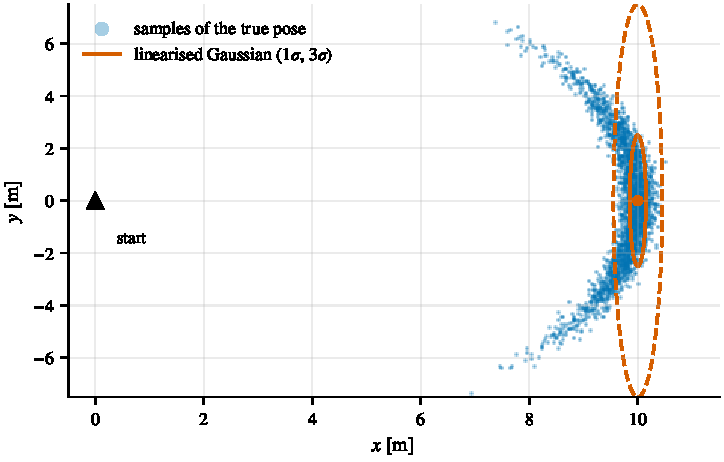
\includegraphics[width=0.84\textwidth]{fig_banana.pdf}
  \caption{A robot drives 10~m with a heading uncertainty of $\sigma_\psi = 0.25$~rad. The true distribution of its final position (samples) is a
  curved ``banana''. The linearized Gaussian (ellipses) matches its first two moments only locally, puts probability where the robot cannot be,
  and misses the curvature. Errors of this kind are why an estimator must keep its errors small, the central design principle of the
  error-state filter.}
  \label{fig:banana}
\end{figure}

\Cref{fig:banana} shows a classic failure. When heading uncertainty is large, positions are distributed along an arc, and the linearized Gaussian
is a poor description: its mean lies outside the arc, and it assigns probability to positions the robot cannot reach. Two remedies exist.
One is to reduce the uncertainty that must be linearized: the error-state filter of \cref{ch:eskf} keeps the estimation error, not the state,
as the quantity it linearizes, and continually resets it to zero. The other is to choose coordinates in which the distribution is close to
Gaussian: a Gaussian on the heading angle and travelled distance, pushed through the exact kinematics, reproduces the banana. \Cref{ch:lie}
develops that idea for rotations, and \cref{ch:nonlinear} presents a third remedy, sigma-point methods that propagate a few carefully chosen
samples instead of a linearization.

\begin{takeaways}
\begin{itemize}
  \item Bayes' rule converts a sensor model $p(z\mid x)$ and a prior $p(x)$ into the posterior $p(x\mid z)$.
  \item Affine maps propagate covariances as $A\Sigma A\T$. This single fact drives prediction, cloning and stacking.
  \item $\E[x\T Ax] = \tr(A\Sigma) + \mu\T A\mu$; the normalized squared error of an $n$-dimensional Gaussian averages to $n$.
  \item In covariance form, marginalization deletes rows and columns and conditioning takes a Schur complement. Information form is the reverse.
  \item Fusing independent Gaussian information adds inverse covariances; the result is a gain-weighted correction.
  \item Monte Carlo errors shrink like $1/\sqrt N$; sums of many small effects are nearly Gaussian.
  \item The squared Mahalanobis distance of an $n$-dimensional Gaussian is $\chi^2_n$: the basis of gating and consistency tests.
  \item Linearization ignores curvature-induced bias and fails when uncertainty is large relative to curvature.
\end{itemize}
\end{takeaways}

\begin{exercises}
  \item A gyro is either healthy (99\%) or faulty (1\%). A self-test flags 98\% of faulty units and 3\% of healthy ones. A unit is flagged; what is
        the probability that it is faulty?
  \item Let $x \sim \N(0, \diag(1, 4))$ and $y = Ax$ with $A$ a rotation by $30^\circ$. Compute $\Cov(y)$ and sketch the $1\sigma$ ellipses of $x$ and $y$.
  \item Prove that $\Sigma_{a|b} \preceq \Sigma_{aa}$: conditioning never increases uncertainty in the Loewner order. When is the inequality an equality?
  \item Derive the information-form marginal $\Lambda_{aa} - \Lambda_{ab}\Lambda_{bb}\inv\Lambda_{ba}$ from \cref{prop:block-inverse} and show that it equals $\Sigma_{aa}\inv$.
  \item Complete the square to derive \eqref{eq:fusion}.
  \item Solve \eqref{eq:map-ls} by setting the gradient to zero, and show that the solution can be written $\hat x = \mu + K(z - H\mu)$ for
        $K = (P\inv + H\T R\inv H)\inv H\T R\inv$.
  \item For $x \sim \N(0, \sigma^2)$ and $y = x^2$, compute the exact mean of $y$ and its first-order linearized prediction. Explain the discrepancy.
  \item What fraction of a 2D Gaussian's probability lies inside its $1\sigma$ Mahalanobis ellipse? (Hint: $P(\chi^2_2 \le 1)$.) Inside its $3\sigma$ ellipse?
  \item Show that $\E[s^4] = 3$ for $s \sim \N(0, 1)$ by integrating by parts.
  \item A Monte Carlo test with $N = 100$ runs finds a sample variance 25\% larger than predicted. Is this evidence of an error at the 5\% level?
\end{exercises}
% Solutions to the exercises of Chapter 5.
\begin{solutions}
  \item Let $F$ = faulty and $T$ = flagged. By the law of total probability $P(T) = 0.98\cdot0.01 + 0.03\cdot0.99 = 0.0098 + 0.0297 = 0.0395$, and by
        Bayes' rule
        \[
          P(F\mid T) = \frac{P(T\mid F)P(F)}{P(T)} = \frac{0.0098}{0.0395} = 0.248 .
        \]
        Only one flagged unit in four is actually faulty. The test is good, but faults are rare: the 3\% false-alarm rate applied to the 99\% of
        healthy units produces three times as many flags as the faulty units do. The prior matters as much as the likelihood.

  \item With $c = \cos30^\circ$ and $s = \sin30^\circ$, \cref{prop:affine} gives
        \[
          \Cov(y) = A\diag(1, 4)A\T = \begin{bmatrix} c^2 + 4s^2 & -3cs \\ -3cs & s^2 + 4c^2 \end{bmatrix}
          = \begin{bmatrix} 1.75 & -1.299 \\ -1.299 & 3.25 \end{bmatrix}.
        \]
        A rotation does not change the eigenvalues, still 1 and 4. The $1\sigma$ ellipse of $x$ has semi-axes 1 along $x_1$ and 2 along $x_2$; that
        of $y$ is the same ellipse rotated by $30^\circ$, its long axis (length 2) along $Ae_2 = (-\tfrac12, \tfrac{\sqrt3}{2})$, at $120^\circ$ from the
        first axis. The negative covariance says that $y_1$ and $y_2$ tend to have opposite signs, as the tilt of the ellipse shows.

  \item The difference is
        \[
          \Sigma_{aa} - \Sigma_{a|b} = \Sigma_{ab}\Sigma_{bb}\inv\Sigma_{ba} = \big(\Sigma_{bb}^{-1/2}\Sigma_{ba}\big)\T\big(\Sigma_{bb}^{-1/2}\Sigma_{ba}\big) \succeq 0,
        \]
        because $x\T\Sigma_{ab}\Sigma_{bb}\inv\Sigma_{ba}x = \|\Sigma_{bb}^{-1/2}\Sigma_{ba}x\|^2 \ge 0$ for every $x$ (with $\Sigma_{bb}^{-1/2}$ any square root of
        $\Sigma_{bb}\inv \succ 0$). Equality holds for all $x$ exactly when $\Sigma_{ba}x = 0$ for all $x$, i.e.\ when $\Sigma_{ab} = 0$: $a$ and $b$ are uncorrelated,
        hence (being jointly Gaussian) independent, and observing $b$ says nothing about $a$.

  \item Order the variables as $(b, a)$, so that $\Lambda$ becomes $\begin{bmatrix}\Lambda_{bb} & \Lambda_{ba}\\ \Lambda_{ab} & \Lambda_{aa}\end{bmatrix}$ and its inverse is
        $\begin{bmatrix}\Sigma_{bb} & \Sigma_{ba}\\ \Sigma_{ab} & \Sigma_{aa}\end{bmatrix}$. By \cref{prop:block-inverse}, with the top-left block $\Lambda_{bb}$ playing the
        role of $A$, the bottom-right block of the inverse is the inverse of the Schur complement:
        \[
          \Sigma_{aa} = \big(\Lambda_{aa} - \Lambda_{ab}\Lambda_{bb}\inv\Lambda_{ba}\big)\inv
          \quad\Longleftrightarrow\quad \Lambda_{aa} - \Lambda_{ab}\Lambda_{bb}\inv\Lambda_{ba} = \Sigma_{aa}\inv .
        \]
        The marginal of $a$ is $\N(\mu_a, \Sigma_{aa})$, whose information matrix is $\Sigma_{aa}\inv$: in information form, marginalization is this Schur
        complement. (The same proposition gives the marginal information vector $\eta_a - \Lambda_{ab}\Lambda_{bb}\inv\eta_b$.)

  \item Up to terms that do not involve $x$, the exponent is
        \[
          -\frac{(x - z_1)^2}{2\sigma_1^2} - \frac{(x - z_2)^2}{2\sigma_2^2}
          = -\frac12\Big(\frac{1}{\sigma_1^2} + \frac{1}{\sigma_2^2}\Big)x^2 + \Big(\frac{z_1}{\sigma_1^2} + \frac{z_2}{\sigma_2^2}\Big)x + \text{const}
          = -\frac{(x - \hat x)^2}{2\sigma^2} + \text{const},
        \]
        where matching the coefficient of $x^2$ gives $1/\sigma^2 = 1/\sigma_1^2 + 1/\sigma_2^2$ and matching that of $x$ gives
        $\hat x/\sigma^2 = z_1/\sigma_1^2 + z_2/\sigma_2^2$. A density proportional to $\exp(-(x - \hat x)^2/2\sigma^2)$ is $\N(\hat x, \sigma^2)$. Finally, with
        $\sigma^2 = \sigma_1^2\sigma_2^2/(\sigma_1^2 + \sigma_2^2)$,
        $\hat x = (\sigma_2^2z_1 + \sigma_1^2z_2)/(\sigma_1^2 + \sigma_2^2) = z_1 + \sigma_1^2(z_2 - z_1)/(\sigma_1^2 + \sigma_2^2)$, the second form of \eqref{eq:fusion}.

  \item The cost $J(x) = (x - \mu)\T P\inv(x - \mu) + (z - Hx)\T R\inv(z - Hx)$ has gradient $2P\inv(x - \mu) - 2H\T R\inv(z - Hx)$. Setting it to zero,
        \[
          \big(P\inv + H\T R\inv H\big)\hat x = P\inv\mu + H\T R\inv z .
        \]
        Write $\hat x = \mu + \delta$ and subtract $(P\inv + H\T R\inv H)\mu$ from both sides: $(P\inv + H\T R\inv H)\,\delta = H\T R\inv(z - H\mu)$, so
        $\hat x = \mu + K(z - H\mu)$ with $K = (P\inv + H\T R\inv H)\inv H\T R\inv$. The Hessian $2(P\inv + H\T R\inv H) \succ 0$ confirms a minimum. By the push-through
        identity $(P\inv + H\T R\inv H)\inv H\T R\inv = PH\T(HPH\T + R)\inv$ this is the Kalman gain of \cref{ch:kf}.

  \item Exactly, $\E[y] = \E[x^2] = \sigma^2$ (and $\Var(y) = \E[x^4] - \sigma^4 = 2\sigma^4$). Linearizing $f(x) = x^2$ at the mean $\mu = 0$ gives $f(0) = 0$ and $J = 2\mu = 0$:
        the predicted mean is $0$ and the predicted variance is $0$, a deterministic $y$. The linearization sees a function that is flat at the
        expansion point and misses the curvature entirely. The second-order correction $\tfrac12f''(\mu)\sigma^2 = \sigma^2$ of \cref{sec:linearization} accounts
        for the whole discrepancy (exactly, because $f$ is quadratic). This is the worst case for an EKF: linearizing at a stationary point of
        the measurement function.

  \item The squared Mahalanobis distance of a 2D Gaussian is $\chi^2_2$, whose density $\tfrac12e^{-\gamma/2}$ integrates to $P(\chi^2_2 \le c) = 1 - e^{-c/2}$.
        The $k\sigma$ ellipse is $d_M^2 = k^2$:
        \[
          P(1\sigma) = 1 - e^{-1/2} = 0.393, \qquad P(2\sigma) = 1 - e^{-2} = 0.865, \qquad P(3\sigma) = 1 - e^{-9/2} = 0.989 .
        \]
        Compare $0.683$, $0.954$ and $0.997$ in one dimension (and $0.199$, $0.739$, $0.971$ in three): the more dimensions, the more likely a sample lies outside
        the ``one-sigma'' region, because it must be close to the mean in every direction at once.

  \item With $\varphi(s) = e^{-s^2/2}/\sqrt{2\pi}$ we have $\varphi'(s) = -s\varphi(s)$. Integrating by parts with $u = s^3$ and $\dd v = s\varphi\,\dd s = -\dd\varphi$,
        \[
          \E[s^4] = \int_{-\infty}^{\infty}s^3\cdot s\varphi(s)\,\dd s = \big[-s^3\varphi(s)\big]_{-\infty}^{\infty} + 3\int_{-\infty}^{\infty}s^2\varphi(s)\,\dd s = 0 + 3\,\E[s^2] .
        \]
        The same step with $u = s$ gives $\E[s^2] = [-s\varphi]_{-\infty}^{\infty} + \int\varphi = 1$. Hence $\E[s^4] = 3$ and $\Var(s^2) = 3 - 1 = 2$, the variance used for $\chi^2_k$.

  \item Under the null hypothesis that the predicted variance is right, $99\,s^2/\sigma^2 \sim \chi^2_{99}$, so the ratio $s^2/\sigma^2$ lies in
        $[\chi^2_{0.025}(99), \chi^2_{0.975}(99)]/99 = [0.741, 1.297]$ with probability 95\% (\cref{app:tables}). The observed ratio $1.25$ is inside the
        interval: \emph{not} significant at the 5\% level (the two-sided $p$-value is about $0.09$). With 100 runs, a variance can be off by 25\%
        without the test noticing; the expected ratio $1.25$ would leave the interval only from about 140 runs, and a 10\% error needs
        roughly a thousand. Monte Carlo variance checks need many runs (Exercise 17.6).
\end{solutions}


\chapter{Random Processes, Spectra and Sensor Noise}
\label{ch:processes}
\chaptermark{Random Processes and Noise} % short running header

\begin{objectives}
\begin{itemize}
  \item Describe noise that evolves in time: random sequences, autocorrelation, stationarity, white noise and random walks.
  \item Understand power spectral densities and why sensor noise is specified in units per $\sqrt{\mathrm{Hz}}$.
  \item Understand continuous-time white noise, its sampling, and aliasing.
  \item Derive how integrated noise grows, and how covariance evolves in a linear stochastic system.
  \item Derive the Allan variance signatures used to identify IMU noise parameters.
  \item Model colored noise with shaping filters, the reason sensor biases become filter states.
\end{itemize}
\end{objectives}

\Cref{ch:prob} dealt with random vectors: a fixed number of uncertain quantities. Sensor noise is a different kind of object: a random
\emph{signal}, a function of time, whose values at different times may or may not be related. This chapter develops the theory of such
random processes, as far as it is needed to understand IMU datasheets, to model sensor errors in a filter, and to discretize those models
correctly.

% ==============================================================================
\section{Random sequences}

\subsection{Definitions}

A \term{random sequence} (discrete-time random process) is a sequence of random variables $x_0, x_1, x_2, \dots$, for example the noise
added to successive IMU samples. One run of the experiment produces one \emph{sample path}; repeating the experiment produces another.
Statistics are taken across this \emph{ensemble} of paths. The \emph{mean function} is $\mu_k = \E[x_k]$ and the \emph{autocovariance}
\begin{equation}
  C(k, j) = \E\big[(x_k - \mu_k)(x_j - \mu_j)\big]
\end{equation}
says how strongly the values at two times are related. A sequence is \term{wide-sense stationary} if its mean is constant and its
autocovariance depends only on the lag, $C(k, j) = C(k - j)$: its statistical character does not change with time.

\subsection{Three fundamental sequences}

\begin{figure}[t]
  \centering
  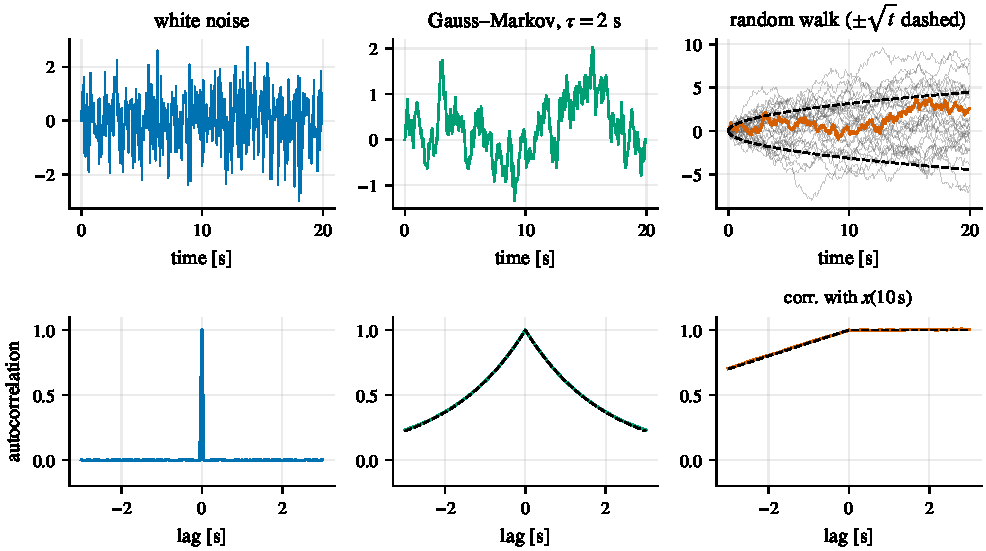
\includegraphics[width=\textwidth]{fig_processes.pdf}
  \caption{Sample paths (top) and autocorrelation functions (bottom) of white noise, a first-order Gauss--Markov sequence with correlation time
  $\tau = 2$~s, and a random walk, all driven by the same white sequence. White noise is uncorrelated with itself at any non-zero lag;
  the Gauss--Markov sequence forgets its past exponentially; the random walk never forgets and its spread grows like $\sqrt t$.}
  \label{fig:processes}
\end{figure}

\paragraph{White noise.} A \term{white sequence} has zero mean and uncorrelated values: $C(k) = \sigma^2$ for $k = 0$ and $0$ otherwise. Each
sample carries no information about the others. The measurement noise of a well-behaved sensor is approximately white.

\paragraph{Random walk.} Summing white noise gives a \term{random walk}: $x_{k+1} = x_k + w_k$, $x_0 = 0$, with $w_k$ white of variance $\sigma^2$. Then
$x_k = \sum_{j<k}w_j$ and, because variances of uncorrelated terms add,
\begin{equation}
  \Var(x_k) = k\sigma^2 .
\end{equation}
The spread grows like $\sqrt k$ without bound, and the sequence is not stationary. Its autocovariance $C(k, j) = \min(k, j)\sigma^2$ shows that
it remembers its whole past. Slowly drifting sensor biases are modeled as random walks.

\paragraph{First-order Gauss--Markov sequence.} Between the two lies $x_{k+1} = ax_k + w_k$ with $|a| < 1$. If the sequence is stationary, taking the
variance of both sides gives $V = a^2V + \sigma^2$, so
\begin{equation}
  \Var(x_k) = \frac{\sigma^2}{1 - a^2}, \qquad C(j) = \frac{\sigma^2}{1 - a^2}\,a^{|j|},
\end{equation}
the second because $x_{k+j} = a^jx_k + (\text{noise uncorrelated with } x_k)$. The sequence forgets its past exponentially, with a
\emph{correlation time} of about $1/(1 - a)$ steps. It is a bounded, slowly varying error: a useful model for biases that wander but do not
diverge, and for many environmental disturbances.

% ==============================================================================
\section{Frequency-domain description}

\subsection{Fourier analysis in brief}

Every reasonable signal is a superposition of sinusoids. The \term{Fourier transform}
\begin{equation}
  X(f) = \int_{-\infty}^{\infty}x(t)\,e^{-i2\pi ft}\,\dd t, \qquad x(t) = \int_{-\infty}^{\infty}X(f)\,e^{i2\pi ft}\,\dd f
\end{equation}
gives the complex amplitude $X(f)$ of the component at frequency $f$ (in Hz). Two facts are all we need. First, Parseval's theorem
$\int|x(t)|^2\dd t = \int|X(f)|^2\dd f$: energy can be counted in time or in frequency. Second, linear time-invariant systems (filters) act
on each frequency independently, multiplying $X(f)$ by a \emph{frequency response} $H(f)$. A low-pass filter has $|H(f)| \approx 1$ at low
frequencies and $|H(f)| \approx 0$ at high ones.

\subsection{Power spectral density}

A random signal has infinite energy (it goes on forever), but finite \emph{power}. Its \term{power spectral density} (PSD) describes how that
power is distributed over frequency.

\begin{definition}[Power spectral density]
For a wide-sense stationary process with autocovariance $C(\tau) = \E[x(t + \tau)x(t)]$ (zero mean), the (two-sided) PSD is
\begin{equation}
  S(f) = \int_{-\infty}^{\infty}C(\tau)\,e^{-i2\pi f\tau}\,\dd\tau .
\end{equation}
\end{definition}

This relation between the autocovariance and the PSD is the \emph{Wiener--Khinchin theorem}. Evaluating the inverse transform at $\tau = 0$ shows
that the variance is the total area under the PSD:
\begin{equation}
  \Var(x) = C(0) = \int_{-\infty}^\infty S(f)\,\dd f .
\end{equation}
So $S(f)\,\dd f$ is the contribution of the frequency band $[f, f + \dd f]$ to the variance, and the PSD has units of $[x]^2/\mathrm{Hz}$. Passing
the process through a filter with frequency response $H(f)$ multiplies its PSD by $|H(f)|^2$.

\begin{pitfall}[one-sided and two-sided PSDs]
Engineers often use a \emph{one-sided} PSD defined only for $f \ge 0$ and equal to twice the two-sided one, so that the variance is
$\int_0^\infty S_1(f)\,\dd f$. Datasheets rarely say which convention they use, and the two differ by a factor of $\sqrt2$ in the noise density.
These notes use the convention of the EuRoC calibration files and of most of the VIO literature: a continuous white noise $w$ with
$\E[w(t)w(s)] = \sigma^2\delta(t - s)$, i.e.\ two-sided PSD $\sigma^2$.
\end{pitfall}

% ==============================================================================
\section{Continuous-time white noise}
\label{sec:ct-noise}

\begin{definition}[Continuous-time white noise]
\index{white noise}
A zero-mean process $w(t) \in \R^n$ is white with \term{noise density} (intensity) $Q_c$ if
$\E[w(t)\,w(s)\T] = Q_c\,\delta(t - s)$, where $\delta$ is the Dirac delta. For a scalar process we write $Q_c = \sigma^2$ and call $\sigma$ the noise
density.
\end{definition}

Continuous white noise is an idealization: its PSD is flat at all frequencies, so its variance $\int S\,\dd f$ is infinite. Physical noise is
white only up to some bandwidth. What makes the idealization useful is that its \emph{integrals} are perfectly well behaved: the integral of
white noise over an interval of length $T$ is a zero-mean random variable with variance
\begin{equation}
  \Var\Big(\int_0^Tw(t)\,\dd t\Big) = \int_0^T\!\!\int_0^T\sigma^2\delta(t - s)\,\dd s\,\dd t = \sigma^2T .
\end{equation}
Since $\delta$ has units of 1/time, $\sigma$ has units of $[w]\cdot\sqrt{\mathrm s} = [w]/\sqrt{\mathrm{Hz}}$. For a gyroscope, $[w] = \mathrm{rad/s}$, so its
noise density is in $\mathrm{rad/s/\sqrt{Hz}}$, the units of \code{gyroscope\_noise\_density} in EuRoC's \code{sensor.yaml}.

\paragraph{From continuous to discrete noise.} A digital sensor reports samples every $\Dt$. If each sample is the average of the
continuous white input over its interval, which an anti-aliasing filter approximates, the sample noise has variance
\begin{equation}
  \Var\Big(\frac1\Dt\int_0^\Dt w(s)\,\dd s\Big) = \frac{\sigma^2}{\Dt}, \qquad \sigma_{\mathrm{discrete}} = \frac{\sigma}{\sqrt{\Dt}} .
  \label{eq:discrete-noise}
\end{equation}
The frequency-domain view agrees: an ideal low-pass filter that keeps the band $|f| < f_s/2$ (with $f_s = 1/\Dt$) passes a variance of
$\int_{-f_s/2}^{f_s/2}\sigma^2\,\dd f = \sigma^2f_s = \sigma^2/\Dt$. Sampling faster does not reduce the noise per unit time; it merely spreads it over
more samples, each noisier. For EuRoC's gyroscope, $\sigma_g = 1.6968\times10^{-4}~\mathrm{rad/s/\sqrt{Hz}}$ at 200~Hz gives a per-sample standard
deviation of $2.4\times10^{-3}$~rad/s.

Conversely, a random walk driven by white noise, $\dot b = w$, gains variance $\sigma^2\Dt$ over a step $\Dt$, so its exact discretization is
$b_{k+1} = b_k + \sqrt{\Dt}\,\sigma\,s_k$ with $s_k \sim \N(0, 1)$. The two conversions go in opposite directions, $\sigma/\sqrt\Dt$ for the sample noise
and $\sigma\sqrt\Dt$ for the walk; confusing them is a classic error in noise simulators.

% ==============================================================================
\section{Sampling and aliasing}

\begin{theorem}[Sampling theorem, Nyquist--Shannon]
\index{sampling theorem}
A signal containing no frequencies at or above $f_s/2$ is completely determined by its samples at rate $f_s$. The frequency $f_s/2$ is the
\term{Nyquist frequency}.
\end{theorem}

\begin{figure}[t]
  \centering
  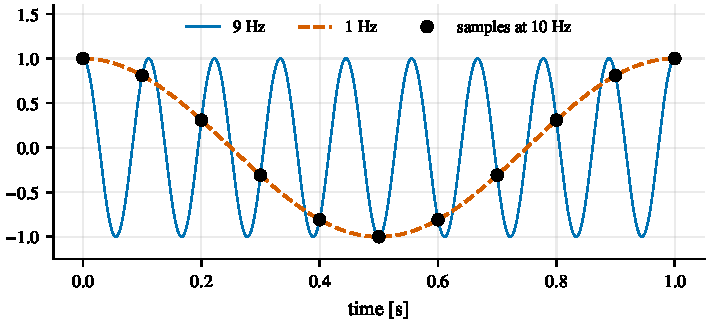
\includegraphics[width=0.9\textwidth]{fig_aliasing.pdf}
  \caption{Aliasing. A 9~Hz sinusoid sampled at 10~Hz (dots) produces exactly the same samples as a 1~Hz sinusoid (dashed). After sampling, the
  two are indistinguishable.}
  \label{fig:aliasing}
\end{figure}

A component at a frequency $f$ above the Nyquist frequency does not disappear when sampled: it masquerades as a lower frequency
$|f - kf_s|$ for the integer $k$ that brings it into $[0, f_s/2]$ (\cref{fig:aliasing}). This \term{aliasing} cannot be undone after sampling, so it
must be prevented before, by an analog or digital \emph{anti-aliasing} low-pass filter. IMUs contain such filters, but strong vibration near
or above the sampling rate (propellers at hundreds of Hz) can still alias into low frequencies and appear as bias-like errors. The same
principle governs images: a camera samples a scene spatially, and an image must be blurred before it is down-sampled, or fine textures turn
into false coarse patterns (\cref{ch:imageproc}).

% ==============================================================================
\section{Integrated noise}

\begin{proposition}[Integrated white noise]
\label{prop:integrated-noise}
Let $w$ be scalar white noise with density $\sigma$. The $m$-fold integral
$I_m(t) = \int_0^t \int_0^{t_1}\cdots\int_0^{t_{m-1}} w(t_m)\,\dd t_m \cdots \dd t_1$ has zero mean and
\begin{equation}
  \Var\big(I_m(t)\big) = \sigma^2\,\frac{t^{2m-1}}{(2m-1)\,\big((m-1)!\big)^2}.
  \label{eq:integrated-noise}
\end{equation}
For $m = 1, 2, 3, 4$ this gives $\sigma^2 t$, $\sigma^2 t^3/3$, $\sigma^2 t^5/20$ and $\sigma^2 t^7/252$.
\end{proposition}
\begin{proof}
By Cauchy's formula for repeated integration (proved by induction, exchanging the order of integration),
$I_m(t) = \int_0^t \frac{(t - s)^{m-1}}{(m-1)!}\,w(s)\,\dd s$. For a weighted integral $\int g(s)w(s)\,\dd s$ of white noise,
$\Var = \iint g(s)g(s')\,\sigma^2\delta(s - s')\,\dd s\,\dd s' = \sigma^2\int g(s)^2\,\dd s$. Here
$\int_0^t (t-s)^{2m-2}\,\dd s/((m-1)!)^2 = t^{2m-1}/((2m-1)((m-1)!)^2)$.
\end{proof}

The single integral $I_1$ is the continuous random walk, or \term{Wiener process}, whose standard deviation grows like $\sqrt t$. Integrating
accelerometer white noise twice into position gives $\sigma_a^2t^3/3$: position uncertainty grows like $t^{3/2}$. Each further integration adds
two powers of $t$ to the variance. \Cref{ch:errordyn} uses this proposition to explain how fast an inertial navigator degrades.

% ==============================================================================
\section{Linear stochastic differential equations}
\label{sec:lyapunov}

Most noise models in navigation are linear systems driven by white noise:
\begin{equation}
  \dot x(t) = F(t)\,x(t) + G(t)\,w(t), \qquad \E[w(t)w(s)\T] = Q_c\,\delta(t - s).
  \label{eq:linear-sde}
\end{equation}
Because white noise is so irregular, such equations are made rigorous by stochastic calculus. For linear systems, however, the results we
need follow from a simple limiting argument.

\begin{proposition}[Mean and covariance propagation]
\label{prop:lyapunov}
\index{Lyapunov equation}
For \eqref{eq:linear-sde}, the mean $m(t) = \E[x(t)]$ and covariance $P(t)$ evolve as
\begin{equation}
  \dot m = Fm, \qquad \dot P = FP + PF\T + GQ_cG\T,
  \label{eq:lyapunov-ode}
\end{equation}
with solution $P(t) = \Phi(t, t_0)P(t_0)\Phi(t, t_0)\T + \int_{t_0}^t\Phi(t, s)G(s)Q_cG(s)\T\Phi(t, s)\T\,\dd s$.
\end{proposition}
\begin{proof}
Over a short interval $h$, $x(t + h) = (I + Fh)x(t) + \int_t^{t+h}Gw\,\dd s + O(h^2)$, and the noise integral is zero-mean with covariance $GQ_cG\T h$ and
uncorrelated with $x(t)$. By \cref{prop:affine}, $P(t + h) = (I + Fh)P(I + Fh)\T + GQ_cG\T h + O(h^2) = P + (FP + PF\T + GQ_cG\T)h + O(h^2)$. Subtract
$P(t)$, divide by $h$ and let $h\to0$. The integral form is verified by differentiating it (\cref{prop:stm}).
\end{proof}

\Cref{eq:lyapunov-ode} is the \emph{Lyapunov differential equation}. The first two terms move and shape the existing uncertainty with the
dynamics; the last term pumps in new uncertainty from the noise. Its integral form over one time step is exactly the discrete process noise
covariance $Q_d$ of the Kalman filter (\cref{ch:linsys,ch:kf}). For a stable time-invariant system, $P$ approaches the solution of the
algebraic Lyapunov equation $0 = FP + PF\T + GQ_cG\T$.

\subsection{The continuous Gauss--Markov process}

The scalar system $\dot x = -x/\tau + w$ with noise density $\sigma$ is the continuous counterpart of the Gauss--Markov sequence. Its stationary
variance solves $0 = -2P/\tau + \sigma^2$:
\begin{equation}
  P_\infty = \frac{\sigma^2\tau}{2}, \qquad C(\Delta t) = P_\infty\,e^{-|\Delta t|/\tau}, \qquad S(f) = \frac{\sigma^2\tau^2}{1 + (2\pi f\tau)^2} .
\end{equation}
(The PSD is the white input PSD $\sigma^2$ times $|H(f)|^2$ for the system's frequency response $H(f) = 1/(i2\pi f + 1/\tau)$; integrating it over all
frequencies returns $P_\infty$.) The autocovariance decays with time constant $\tau$, and the PSD is flat up to the corner frequency $1/(2\pi\tau)$ and
falls off beyond it. Its exact discretization over $\Dt$ is $x_{k+1} = e^{-\Dt/\tau}x_k + w_k$ with $\Var(w_k) = P_\infty(1 - e^{-2\Dt/\tau})$. As
$\tau\to\infty$ it becomes a random walk; as $\tau\to0$ with the low-frequency level $\sigma^2\tau^2$ of its PSD held fixed, it becomes white noise.

% ==============================================================================
\section{Colored noise and state augmentation}

A Kalman filter assumes that its process and measurement noises are white. When a disturbance is \emph{colored} (correlated in time), the
standard remedy is to model it as the output of a linear system driven by white noise, a \emph{shaping filter}, and to add the state of that
system to the filter state. A sensor bias that drifts as a random walk is exactly this: $b$ is colored, but $\dot b = w_b$ is white-driven, so
$b$ becomes part of the state. This is why IMU biases appear in the state vector of every inertial filter (\cref{ch:imu}). Ignoring the
correlation, and treating a slowly varying error as white, makes the filter believe that errors average out when they do not, and leads to
overconfidence.

% ==============================================================================
\section{The Allan variance}
\label{sec:allan}

How are the noise densities of a sensor measured? Record it at rest for hours and compute its \term{Allan variance}, a tool developed for
characterizing atomic clocks that separates noise processes by their time scale.

\begin{definition}[Allan variance]
Split a record of rate samples $y(t)$ into consecutive clusters of duration $\tau$, and let $\bar y_k(\tau)$ be the average over cluster $k$. The
Allan variance is half the mean squared difference of consecutive cluster averages:
\begin{equation}
  \sigma_A^2(\tau) = \tfrac12\,\E\big[(\bar y_{k+1}(\tau) - \bar y_k(\tau))^2\big] .
\end{equation}
\end{definition}

In practice it is computed from the integrated signal $\theta(t) = \int_0^ty$ (for a gyroscope, the angle), since
$\bar y_{k+1} - \bar y_k = (\theta_{k+2} - 2\theta_{k+1} + \theta_k)/\tau$ with $\theta_j = \theta(j\tau)$. The \emph{overlapping} estimator averages over all
starting times rather than only disjoint clusters, which uses the data more efficiently.

\begin{proposition}[Allan variance signatures]
For white noise of density $\sigma$, $\sigma_A^2(\tau) = \sigma^2/\tau$. For a random walk $\dot b = w_b$ with density $\sigma_b$, $\sigma_A^2(\tau) = \sigma_b^2\tau/3$.
\end{proposition}
\begin{proof}
\emph{White noise.} Each cluster average is an integral of white noise divided by $\tau$, with variance $\sigma^2\tau/\tau^2 = \sigma^2/\tau$; consecutive
averages involve disjoint intervals and are uncorrelated, so their difference has variance $2\sigma^2/\tau$, and half of it is $\sigma^2/\tau$.
\emph{Random walk.} Write $b(t) = \int_0^tw_b$. The difference of two consecutive cluster averages is
$D = \frac1\tau\int_\tau^{2\tau}b\,\dd t - \frac1\tau\int_0^\tau b\,\dd t$. Substituting $b$ and exchanging the order of integration expresses $D$ as
$\frac1\tau\int_0^{2\tau}h(s)w_b(s)\,\dd s$ with $h(s) = s$ for $s \le \tau$ and $h(s) = 2\tau - s$ for $s > \tau$ (a triangular weight). Its variance is
$\frac{\sigma_b^2}{\tau^2}\big(\int_0^\tau s^2\dd s + \int_\tau^{2\tau}(2\tau - s)^2\dd s\big) = \frac{2}{3}\sigma_b^2\tau$, and half of it is $\sigma_b^2\tau/3$.
\end{proof}

On a log-log plot of the \emph{Allan deviation} $\sigma_A(\tau)$, independent noise processes therefore appear as straight lines with
characteristic slopes:
\begin{center}\small
\begin{tabular}{@{}l l l@{}}
\toprule
Process & $\sigma_A^2(\tau)$ & slope of $\sigma_A$ \\
\midrule
quantization noise & $3Q^2/\tau^2$ & $-1$ \\
white noise (density $\sigma$) & $\sigma^2/\tau$ & $-\tfrac12$ \\
bias instability ($B$) & $\approx (0.664 B)^2$ & $0$ \\
bias random walk (density $\sigma_b$) & $\sigma_b^2\tau/3$ & $+\tfrac12$ \\
rate ramp ($R$) & $R^2\tau^2/2$ & $+1$ \\
\bottomrule
\end{tabular}
\end{center}
The white-noise density is read off the $-\tfrac12$ line at $\tau = 1$~s, and the random-walk density off the $+\tfrac12$ line at $\tau = 3$~s. The
minimum of the curve marks the averaging time beyond which a stationary sensor's bias starts to wander; its height is related to the
\emph{bias instability}, a flicker-noise floor that neither white noise nor a random walk describes exactly.

\begin{figure}[t]
  \centering
  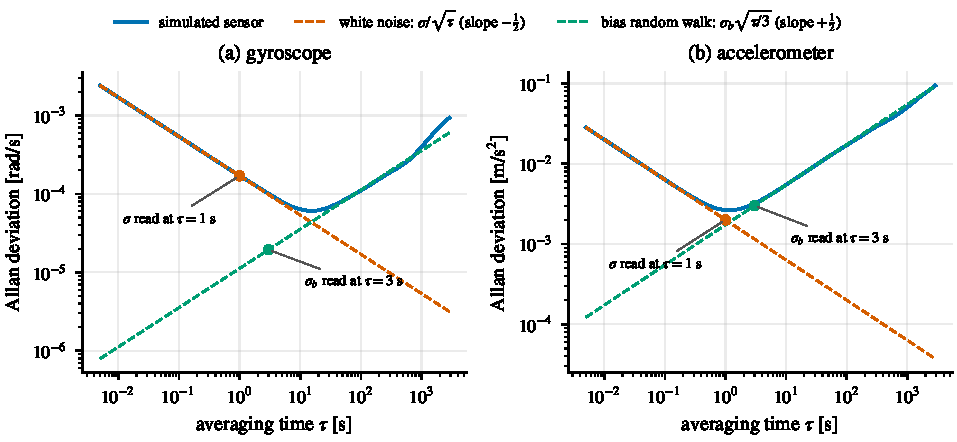
\includegraphics[width=\textwidth]{fig_allan.pdf}
  \caption{Allan deviation of a simulated 4-hour static recording with EuRoC's IMU noise parameters. The $-\tfrac12$ slope of white noise
  dominates short averaging times and the $+\tfrac12$ slope of the bias random walk dominates long ones. Reading the asymptotes at
  $\tau = 1$~s and $\tau = 3$~s recovers the densities.}
  \label{fig:allan}
\end{figure}

\Cref{fig:allan} shows the procedure on simulated data with the EuRoC parameters of \cref{ch:imu}. On real sensors, a flat bias-instability
region appears near the minimum, which the random-walk model only approximates. The IEEE standard procedure~\cite{ieee952} and El-Sheimy et
al.~\cite{elsheimy2008allan} give practical details.

\begin{takeaways}
\begin{itemize}
  \item White noise is uncorrelated in time; a random walk is its running sum, with variance growing linearly; a Gauss--Markov process
        forgets its past exponentially.
  \item The PSD distributes a process's variance over frequency; noise densities are square roots of PSDs, in units per $\sqrt{\mathrm{Hz}}$.
  \item Sampling white noise of density $\sigma$ at period $\Dt$ gives per-sample noise $\sigma/\sqrt\Dt$; a random walk gains $\sigma_b\sqrt\Dt$ per step.
  \item Frequencies above Nyquist alias; filter before you sample or down-sample.
  \item The $m$-fold integral of white noise has variance growing like $t^{2m-1}$.
  \item Covariance in a linear stochastic system obeys $\dot P = FP + PF\T + GQ_cG\T$.
  \item Colored noise is modeled with a shaping filter whose state joins the filter state: this is why biases are states.
  \item The Allan deviation separates white noise (slope $-\tfrac12$, read at 1~s) from bias random walk (slope $+\tfrac12$, read at 3~s).
\end{itemize}
\end{takeaways}

\begin{exercises}
  \item Show that the autocovariance of a random walk is $C(k, j) = \min(k, j)\,\sigma^2$.
  \item For the Gauss--Markov sequence with $a = 0.99$ and $\sigma = 1$, compute the stationary standard deviation and the lag at which the
        correlation drops below $1/e$.
  \item A 1~kHz accelerometer has white noise of $2\times10^{-3}~\mathrm{m/s^2/\sqrt{Hz}}$. What is the standard deviation of a single sample? Of the average
        of 1000 consecutive samples? Of a single sample of the same sensor read at 100~Hz?
  \item A 105~Hz vibration is sampled at 100~Hz. At what frequency does it appear?
  \item Verify \cref{prop:integrated-noise} by Monte Carlo for $m = 2$ and $m = 3$, simulating at 200~Hz for 10~s with 1000 runs.
  \item Solve the Lyapunov equation for the double integrator $\dot p = v$, $\dot v = w$ with $P(0) = 0$ and verify that $P_{pp}(t) = \sigma^2t^3/3$.
  \item Derive the stationary variance and the exact discretization of the continuous Gauss--Markov process.
  \item Simulate 2 hours of a gyro with EuRoC parameters, compute the overlapping Allan deviation, and recover $\sigma_g$ and $\sigma_{b_g}$ from the
        asymptotes. How long a recording is needed to estimate $\sigma_{b_g}$ to 10\%?
\end{exercises}

\chapter{Rotations, Quaternions and Rigid-Body Kinematics}
\label{ch:rotations}
\chaptermark{Rotations and Quaternions} % short running header

\begin{objectives}
\begin{itemize}
  \item Read and write frame-annotated transformations such as $R_{wb}$, $p_{wb}$ and $T_{bc}$ without ambiguity, and catch frame bugs
        with the adjacency rule.
  \item Understand rotations in the plane, then in space: rotation matrices, axis-angle and Rodrigues' formula.
  \item Understand Euler angles, intrinsic versus extrinsic sequences, their conversions, and why they are banned from the estimator.
  \item Derive Hamilton quaternion algebra and its rotation formula; convert between quaternions and matrices; interpolate; and
        translate formulas from the JPL convention.
  \item Derive the kinematics of rotating bodies: $\dot R = R\sx{\omega}$, $\dot q = \tfrac12 q\qprod[0,\omega]$, the transport theorem and the Coriolis
        acceleration, and quantify the effects of the Earth's rotation.
\end{itemize}
\end{objectives}

% ==============================================================================
\section{Frames and notation}

A \term{frame} is an origin together with three orthonormal, right-handed axes. Three frames appear in this project (\cref{fig:frames}).

\begin{convention}[frames, AGENTS.md C1]
\begin{itemize}
  \item $W$, the \textbf{world} frame: fixed, gravity-aligned with $z$ pointing up, the frame of the ground truth (EuRoC calls it
        \code{R}). Gravity is $g_w = [0, 0, -9.81]\T~\mathrm{m/s^2}$.
  \item $B$, the \textbf{body} frame: the IMU frame \code{imu0} (EuRoC's \code{S} in \code{imu0}).
  \item $C$, the left \textbf{camera} frame \code{cam0}: origin at the optical center, $z$ along the optical axis, $x$ to the right and $y$
        down in the image.
\end{itemize}
$R_{wb}$ (or $q_{wb}$) maps body-frame coordinates to world-frame coordinates, $v_w = R_{wb}v_b$. $p_{wb}$ is the position of the origin of $B$
expressed in $W$. $v_{wb}$ is the velocity of $B$ relative to $W$, expressed in $W$. $T_{bc} = (R_{bc}, p_{bc})$ maps camera points into the body
frame, $p_b = R_{bc}p_c + p_{bc}$; it is \code{T\_BS} from \code{cam0/sensor.yaml}. A world-to-body rotation is never used as a state.
\end{convention}

\begin{figure}[t]
\centering
\begin{tikzpicture}[scale=1.0]
  \coordinate (W) at (0,0);
  \draw[frameaxis, plotorange] (W) -- ++(1.4,0) node[right] {$x_w$};
  \draw[frameaxis, plotgreen] (W) -- ++(0.75,0.6) node[above right] {$y_w$};
  \draw[frameaxis, plotblue] (W) -- ++(0,1.4) node[above] {$z_w$};
  \node[below left] at (W) {$W$};
  \draw[->, thick, black!60] (-0.6,1.0) -- ++(0,-0.8) node[midway, left] {$g$};
  \coordinate (B) at (5.2,2.2);
  \begin{scope}[shift={(B)}, rotate=25]
    \draw[fill=primarylight, draw=primary, rounded corners=2pt] (-0.55,-0.25) rectangle (0.55,0.25);
    \draw[frameaxis, plotorange] (0,0) -- (1.3,0) node[right] {$x_b$};
    \draw[frameaxis, plotgreen] (0,0) -- (0.65,0.55) node[above right] {$y_b$};
    \draw[frameaxis, plotblue] (0,0) -- (0,1.3) node[above] {$z_b$};
    \node[below left] at (-0.2,-0.25) {$B$ (IMU)};
    \coordinate (C) at (2.0,-1.3);
    \draw[fill=white, draw=primary] ($(C)+(-0.15,0.15)$) rectangle ($(C)+(0.15,-0.15)$);
    \draw[frameaxis, plotblue] (C) -- ++(0,-0.9) node[below] {$z_c$};
    \draw[frameaxis, plotorange] (C) -- ++(0.8,0) node[right] {$x_c$};
    \draw[frameaxis, plotgreen] (C) -- ++(-0.45,-0.35) node[left] {$y_c$};
    \node[above right] at ($(C)+(0.1,0.1)$) {$C$};
    \draw[->, thick, conv] (0.3,-0.3) to[bend right=20] node[midway, below left=-1pt] {$T_{bc}$} ($(C)+(-0.2,0.05)$);
  \end{scope}
  \draw[->, thick, primary, dashed] (W) -- (B) node[midway, above left] {$p_{wb}$, $R_{wb}$};
\end{tikzpicture}
\caption{The world frame $W$ (gravity-aligned, $z$ up), the body/IMU frame $B$ moving with the vehicle, and the camera frame $C$ rigidly
attached to the body through the constant extrinsic calibration $T_{bc}$.}
\label{fig:frames}
\end{figure}

\subsection{Reading subscripts}

The naming rule \code{<quantity>\_<to><from>} makes products self-checking. $R_{wb}$ takes a vector \emph{from} $B$ \emph{to} $W$. Composition
chains frames like dominoes:
\begin{equation}
  R_{wc} = R_{wb}\,R_{bc}, \qquad v_w = R_{wb}\,R_{bc}\,v_c .
\end{equation}

\begin{keyidea}[the adjacency rule]
\index{adjacency rule}
In a valid product, adjacent subscripts match: $R_{w\underline{b}}\,R_{\underline{b}c}$. A product such as $R_{wb}R_{cb}$ has mismatched neighbors and is
a bug. The fix is a transpose, $R_{wb}R_{cb}\T = R_{wb}R_{bc}$, since $R_{bc} = R_{cb}\inv = R_{cb}\T$. Apply the rule to every line of code that
multiplies rotations or transforms points.
\end{keyidea}

\subsection{Active and passive views}

A rotation matrix can be read in two ways. In the \emph{passive} view, $R_{wb}$ re-expresses the same physical vector in another frame:
$v_w$ and $v_b$ are coordinates of one arrow (\cref{sec:orthogonal-matrices}). In the \emph{active} view, $R_{wb}$ rotates the world axes
onto the body axes: its columns are the body axes $x_b, y_b, z_b$ expressed in world coordinates. Both readings describe the same matrix:
\begin{equation}
  R_{wb} = \begin{bmatrix} x_b^{(w)} & y_b^{(w)} & z_b^{(w)} \end{bmatrix}.
\end{equation}
This gives a quick sanity check when debugging: the third column of $R_{wb}$ is the body $z$-axis in world coordinates. For a level
vehicle whose $z$-axis points up, it is $[0,0,1]\T$; its third row is the world vertical expressed in the body frame.

% ==============================================================================
\section{Rotations in the plane}

Planar rotations contain most of the ideas of this chapter in their simplest form. The rotation by $\theta$ is (\cref{ex:rot2d})
\begin{equation}
  R(\theta) = \begin{bmatrix} \cos\theta & -\sin\theta \\ \sin\theta & \cos\theta \end{bmatrix}.
\end{equation}
Rotations compose by adding angles, $R(\alpha)R(\beta) = R(\alpha + \beta)$ (multiply out and use the angle-addition formulas), so planar
rotations commute. The angle is a perfect coordinate: $R(\theta)$ is determined by $\theta$, and every planar rotation is $R(\theta)$ for a
$\theta$ that is unique up to multiples of $2\pi$. The only subtlety is wrap-around: angles must be compared modulo $2\pi$, which is why the
difference between two headings is computed as $\atantwo(\sin(\theta_2 - \theta_1), \cos(\theta_2 - \theta_1))$ rather than $\theta_2 - \theta_1$.

Identifying the plane with the complex numbers, rotation by $\theta$ is multiplication by $e^{i\theta} = \cos\theta + i\sin\theta$. Unit complex
numbers compose by multiplication, and their angles add. Quaternions (\cref{sec:quaternions}) are the three-dimensional generalization of
this idea, with one crucial difference: in three dimensions, rotations do not commute.

% ==============================================================================
\section{Rotation matrices and \texorpdfstring{$\SO$}{SO(3)}}

\begin{definition}[Special orthogonal group]
\index{special orthogonal group}
$\SO = \{ R \in \R^{3\times3} : R\T R = I,\ \det R = +1 \}$.
\end{definition}

Orthogonality ($R\T R = I$) means $R$ preserves lengths and angles; $\det R = +1$ excludes reflections, which would turn a right-handed
frame into a left-handed one (\cref{sec:orthogonal-matrices}). The set is closed under multiplication and inversion, $R\inv = R\T$, so it is
a \emph{group}. A rotation matrix has nine entries but only three degrees of freedom: orthonormality imposes six constraints (three unit
lengths, three orthogonalities). This redundancy is why $\SO$ is a curved three-dimensional surface inside the nine-dimensional space of
matrices rather than a vector space; the sum of two rotation matrices is not a rotation matrix.

The elementary rotations about the coordinate axes follow from the planar case:
\begin{equation}
  R_x(\alpha) = \begin{bmatrix} 1 & 0 & 0 \\ 0 & c_\alpha & -s_\alpha \\ 0 & s_\alpha & c_\alpha \end{bmatrix},\quad
  R_y(\alpha) = \begin{bmatrix} c_\alpha & 0 & s_\alpha \\ 0 & 1 & 0 \\ -s_\alpha & 0 & c_\alpha \end{bmatrix},\quad
  R_z(\alpha) = \begin{bmatrix} c_\alpha & -s_\alpha & 0 \\ s_\alpha & c_\alpha & 0 \\ 0 & 0 & 1 \end{bmatrix},
\end{equation}
with $c_\alpha = \cos\alpha$, $s_\alpha = \sin\alpha$. (The signs of $R_y$ look reversed but are not: in the $z$-$x$ plane, ordered cyclically
after $y$, it is the usual planar rotation.) Rotations in space do not commute: $R_x(90^\circ)R_y(90^\circ) \ne R_y(90^\circ)R_x(90^\circ)$. Try it
with a book.

\section{Axis-angle and Rodrigues' formula}

By Euler's theorem (\cref{thm:euler-axis}), every rotation is a rotation by some angle $\theta \in [0, \pi]$ about some unit axis $u$. The pair
$(u, \theta)$ is the \term{axis-angle} representation, and $\phi = \theta u \in \R^3$ is the \term{rotation vector}: its direction is the axis and its
length the angle. The rotation vector is the central object of \cref{ch:lie}.

\begin{theorem}[Rodrigues' rotation formula]
\label{thm:rodrigues}
\index{Rodrigues' formula}
The rotation by angle $\theta$ about the unit axis $u$ is
\begin{equation}
  R = I + \sin\theta\,\sx{u} + (1 - \cos\theta)\,\sx{u}^2
    = \cos\theta\, I + (1-\cos\theta)\,u u\T + \sin\theta\,\sx{u}.
  \label{eq:rodrigues}
\end{equation}
\end{theorem}
\begin{proof}[Geometric proof]
Split any vector into components parallel and perpendicular to the axis (\cref{prop:projection-line}), $v = v_\parallel + v_\perp$ with
$v_\parallel = u u\T v$. Rotation leaves $v_\parallel$ unchanged and rotates $v_\perp$ by $\theta$ within the plane spanned by $v_\perp$ and
$u \times v_\perp = u \times v$ (a vector of the same length, rotated $90^\circ$ about $u$):
\begin{equation*}
  Rv = v_\parallel + \cos\theta\, v_\perp + \sin\theta\, u \times v .
\end{equation*}
Substituting $v_\perp = v - uu\T v = -\sx{u}^2 v$ (from \eqref{eq:skew-sq} with $\|u\|=1$) and $u \times v = \sx{u}v$ gives
$Rv = (I + \sin\theta\sx{u} + (1 - \cos\theta)\sx{u}^2)v$.
\end{proof}
\begin{proof}[Algebraic proof]
The rotation about $u$ at unit angular rate satisfies $\dot R = \sx{u} R$ (\cref{sec:rot-kinematics}), so $R(\theta) = \exp(\theta\sx{u})$ by
\cref{thm:lti-solution}. With $\sx{u}^3 = -\sx{u}$ from \eqref{eq:skew-cube}, all odd powers of $\sx{u}$ are $\pm\sx{u}$ and all even powers
(except the zeroth) are $\pm\sx{u}^2$, so the exponential series regroups as
\begin{equation*}
  \exp(\theta\sx{u}) = I + \Big(\theta - \tfrac{\theta^3}{3!} + \tfrac{\theta^5}{5!} - \cdots\Big)\sx{u}
     + \Big(\tfrac{\theta^2}{2!} - \tfrac{\theta^4}{4!} + \cdots\Big)\sx{u}^2,
\end{equation*}
and the two series are $\sin\theta$ and $1 - \cos\theta$.
\end{proof}

Two consequences of \eqref{eq:rodrigues} recover $(u, \theta)$ from $R$. Taking the trace (using $\tr\sx{u} = 0$ and $\tr\sx{u}^2 = -2$) and the
skew-symmetric part,
\begin{equation}
  \tr R = 1 + 2\cos\theta, \qquad R - R\T = 2\sin\theta\,\sx{u}.
  \label{eq:trace-angle}
\end{equation}
\Cref{ch:lie} shows that \emph{how} these are combined numerically matters a great deal.

\begin{worked}[a quarter turn]
Rotate by $\theta = 90^\circ$ about $u = e_z$: $\sx{e_z} = \begin{bmatrix}0 & -1 & 0\\1 & 0 & 0\\0 & 0 & 0\end{bmatrix}$ and
$\sx{e_z}^2 = \diag(-1, -1, 0)$, so \eqref{eq:rodrigues} gives $R = \begin{bmatrix}0 & -1 & 0\\ 1 & 0 & 0\\ 0 & 0 & 1\end{bmatrix} = R_z(90^\circ)$, which
sends $e_x$ to $e_y$, as a counter-clockwise quarter turn about $z$ should. Its trace is $1 = 1 + 2\cos90^\circ$.
\end{worked}

% ==============================================================================
\section{Euler angles}

\subsection{Definition and the two readings}

\term{Euler angles} describe a rotation as three successive rotations about coordinate axes. The aerospace yaw-pitch-roll ($ZYX$)
convention writes
\begin{equation}
  R_{wb} = R_z(\psi)\,R_y(\vartheta)\,R_x(\varphi),
  \label{eq:zyx}
\end{equation}
with yaw $\psi$, pitch $\vartheta$ and roll $\varphi$. The same product can be read in two ways, which are a constant source of confusion:
\begin{itemize}
  \item \emph{Intrinsic} (rotating axes): start aligned with the world, yaw by $\psi$ about $z$, then pitch by $\vartheta$ about the \emph{new} $y$-axis,
        then roll by $\varphi$ about the \emph{newest} $x$-axis. This is how a pilot thinks.
  \item \emph{Extrinsic} (fixed axes): roll by $\varphi$ about the world $x$-axis, then pitch by $\vartheta$ about the world $y$-axis, then yaw by $\psi$ about
        the world $z$-axis.
\end{itemize}
Both readings produce the same matrix \eqref{eq:zyx}; the intrinsic sequence $z, y', x''$ equals the extrinsic sequence $x, y, z$ in reverse
order. Twelve different axis sequences are in use, and each library documents its own. Always check the convention against a known example
before trusting a conversion.

\subsection{Conversions}

Multiplying out \eqref{eq:zyx} gives the third row of $R$ as $(-\sin\vartheta,\ \cos\vartheta\sin\varphi,\ \cos\vartheta\cos\varphi)$ and the first column as
$\cos\vartheta(\cos\psi, \sin\psi, \cdot)$. Hence
\begin{equation}
  \vartheta = \atantwo\big(-R_{31},\ \sqrt{R_{11}^2 + R_{21}^2}\big), \qquad
  \varphi = \atantwo(R_{32},\ R_{33}), \qquad
  \psi = \atantwo(R_{21},\ R_{11}) .
\end{equation}
When $\cos\vartheta = 0$ ($\vartheta = \pm90^\circ$), the formulas for $\varphi$ and $\psi$ become $\atantwo(0, 0)$: only their sum or difference is determined.

\subsection{Gimbal lock}

The relation between the body angular velocity measured by a gyroscope and the rates of the Euler angles is
\begin{equation}
  \begin{bmatrix} \dot\varphi \\ \dot\vartheta \\ \dot\psi \end{bmatrix}
  = \begin{bmatrix}
      1 & \sin\varphi\tan\vartheta & \cos\varphi\tan\vartheta \\
      0 & \cos\varphi & -\sin\varphi \\
      0 & \sin\varphi/\cos\vartheta & \cos\varphi/\cos\vartheta
    \end{bmatrix} \omega_b ,
  \label{eq:euler-rates}
\end{equation}
obtained by differentiating \eqref{eq:zyx} and comparing with $\sx{\omega_b} = R\T\dot R$ (\cref{sec:rot-kinematics}). At $\vartheta = \pm90^\circ$ the
matrix blows up. Geometrically, when the nose points straight up, yaw and roll rotate about the same physical axis, so the three angles no
longer describe three independent motions. This is \term{gimbal lock}, named after mechanical gimbal platforms that physically jam in this
configuration. Near the singularity, small angular velocities produce enormous Euler-angle rates, and a filter that linearizes in Euler
angles becomes numerically meaningless.

\begin{convention}[AGENTS.md C2]
Euler angles never appear in the estimator. They may appear only in telemetry and plots.
\end{convention}

No three-parameter representation of $\SO$ is free of singularities everywhere: a topological fact (the space $\SO$ cannot be covered by a
single chart). The solution adopted by modern estimators is to store attitude in a singularity-free \emph{redundant} representation (a unit
quaternion or a rotation matrix) and to use three parameters only for \emph{small} deviations around the current estimate, where no
singularity is near. That is the content of \cref{ch:lie}.

% ==============================================================================
\section{Quaternions}
\label{sec:quaternions}

\subsection{Quaternion algebra}

\index{quaternion}
A \term{quaternion} is a four-component number $q = w + x\,i + y\,j + z\,k$, written as a scalar part and a vector part, $q = [w,\ v]$ with
$v = (x,y,z)\T$. Hamilton's multiplication rules for the three imaginary units are
\begin{equation}
  i^2 = j^2 = k^2 = ijk = -1,
\end{equation}
from which $ij = k = -ji$, $jk = i = -kj$ and $ki = j = -ik$. (For example, multiplying $ijk = -1$ on the right by $k$ gives $ij(-1) = -k$.)
Expanding the product of two quaternions term by term with these rules and collecting the scalar and vector parts gives
\begin{equation}
  p \qprod q = \begin{bmatrix} p_w q_w - p_v\T q_v \\ p_w q_v + q_w p_v + p_v \times q_v \end{bmatrix}.
  \label{eq:qprod}
\end{equation}
The products of imaginary units produce exactly the components of the cross product, which makes the product non-commutative:
$p\qprod q - q\qprod p = [0,\ 2p_v\times q_v]$. It is associative. Because it is linear in each factor, it can be written with matrices,
\begin{equation}
  p\qprod q = [p]_L\, q = [q]_R\, p, \qquad
  [p]_L = \begin{bmatrix} p_w & -p_v\T \\ p_v & p_w I + \sx{p_v} \end{bmatrix}, \quad
  [q]_R = \begin{bmatrix} q_w & -q_v\T \\ q_v & q_w I - \sx{q_v} \end{bmatrix},
\end{equation}
where quaternions are treated as 4-vectors $[q_w;\ q_v]$.

The \emph{conjugate} is $q^* = [w,\ -v]$ and the \emph{norm} is $\|q\| = \sqrt{w^2 + \|v\|^2}$. By \eqref{eq:qprod}, $q\qprod q^* = [\|q\|^2,\ 0]$, so the
inverse is $q\inv = q^*/\|q\|^2$. Conjugation reverses products, $(p\qprod q)^* = q^*\qprod p^*$, and norms multiply, $\|p\qprod q\| = \|p\|\|q\|$
(because $\|p\qprod q\|^2 = p\qprod q\qprod q^*\qprod p^* = \|q\|^2\,p\qprod p^* = \|p\|^2\|q\|^2$). Consequently the product of two \emph{unit}
quaternions is a unit quaternion: unit quaternions form a group, the three-dimensional sphere $S^3 \subset \R^4$.

\subsection{Unit quaternions represent rotations}

Identify a vector $a \in \R^3$ with the \emph{pure} quaternion $[0, a]$.

\begin{theorem}[Rotation by a unit quaternion]
\label{thm:quat-rotation}
For a unit quaternion $q = [w, v]$, the map $a \mapsto q\qprod[0, a]\qprod q^*$ sends pure quaternions to pure quaternions and acts on $a$ as the rotation
matrix
\begin{equation}
  R(q) = (w^2 - v\T v)\,I + 2\,v v\T + 2w\,\sx{v}
  = \begin{bmatrix}
    1 - 2(y^2 + z^2) & 2(xy - wz) & 2(xz + wy) \\
    2(xy + wz) & 1 - 2(x^2 + z^2) & 2(yz - wx) \\
    2(xz - wy) & 2(yz + wx) & 1 - 2(x^2 + y^2)
  \end{bmatrix}.
  \label{eq:quat-to-rot}
\end{equation}
The unit quaternion of a rotation by $\theta$ about the unit axis $u$ is
\begin{equation}
  q = \big[\cos(\theta/2),\ \sin(\theta/2)\,u\big].
  \label{eq:quat-axis-angle}
\end{equation}
\end{theorem}
\begin{proof}
By \eqref{eq:qprod}, $[0, a]\qprod q^* = [a\T v,\ wa - a\times v]$. Multiplying on the left by $q = [w, v]$:
the scalar part is $w\,a\T v - v\T(wa - a\times v) = 0$ (since $v\T(a\times v) = 0$), and the vector part is
$w(wa - a\times v) + (a\T v)v + v\times(wa - a\times v) = w^2a + 2w\,v\times a + (v\T a)v - v\times(a\times v)$. With the BAC--CAB rule,
$v\times(a\times v) = a\,(v\T v) - v\,(v\T a)$, so the vector part is $(w^2 - v\T v)a + 2(v\T a)v + 2w\,v\times a$, which is \eqref{eq:quat-to-rot}. This
matrix is orthogonal with determinant one (it preserves norms, because quaternion norms multiply, and depends continuously on $q$, equal to
$I$ at $q = [1, 0]$). For \eqref{eq:quat-axis-angle}, substitute $w = \cos\frac\theta2$, $v = \sin\frac\theta2 u$ and use the double-angle identities
$w^2 - v\T v = \cos\theta$, $2\sin^2\frac\theta2 = 1 - \cos\theta$ and $2\sin\frac\theta2\cos\frac\theta2 = \sin\theta$; the result is the second form of
Rodrigues' formula \eqref{eq:rodrigues}.
\end{proof}

The \emph{half} angle in \eqref{eq:quat-axis-angle} is the most common source of factor-of-two bugs. It arises because $q$ appears twice in the
sandwich product $q \qprod [0,a] \qprod q^*$, each occurrence contributing half of the rotation.

\begin{keyidea}[double cover]
\index{double cover}
$q$ and $-q$ give the same $R(q)$, since \eqref{eq:quat-to-rot} is quadratic in $q$. Every rotation has exactly two unit quaternions, at opposite
points of the sphere $S^3$. They correspond to rotating by $\theta$ about $u$, or by $2\pi - \theta$ about $-u$. Code that compares, averages,
interpolates or takes logarithms of quaternions must account for this. The project canonicalizes to $w \ge 0$ before taking $\Log_q$
(AGENTS.md C2).
\end{keyidea}

\subsection{Composition}

Because $(p\qprod q)\qprod[0, a]\qprod(p\qprod q)^* = p\qprod\big(q\qprod[0, a]\qprod q^*\big)\qprod p^*$, the Hamilton product composes rotations in the same order
as matrix multiplication:
\begin{equation}
  R(p \qprod q) = R(p)\,R(q), \qquad q_{wc} = q_{wb}\qprod q_{bc} \ \leftrightarrow\ R_{wc} = R_{wb}R_{bc}.
\end{equation}
The adjacency rule therefore applies to quaternions unchanged. Composing quaternions costs 16 multiplications and 12 additions, against 27 and
18 for matrices, and renormalizing a quaternion is trivial compared with re-orthogonalizing a matrix. These are the practical reasons to
store attitude as a quaternion.

\begin{worked}[composing two quarter turns]
The quarter turn about $z$ is $q_z = [\cos45^\circ,\ \sin45^\circ e_z] = \frac{1}{\sqrt2}[1, (0,0,1)]$, and about $x$ it is
$q_x = \frac{1}{\sqrt2}[1, (1,0,0)]$. By \eqref{eq:qprod}, $q_z\qprod q_x = \tfrac12\big[1,\ (1, 0, 1) + e_z\times e_x\big] = \tfrac12[1, (1, 1, 1)]$: a rotation by
$2\arccos\frac12 = 120^\circ$ about $(1,1,1)/\sqrt3$. (Check: it cycles the axes, $x\to y\to z\to x$.) In the other order,
$q_x\qprod q_z = \tfrac12[1, (1, -1, 1)]$, a different rotation.
\end{worked}

\subsection{Converting a rotation matrix to a quaternion}

Inverting \eqref{eq:quat-to-rot} naively via $w = \tfrac12\sqrt{1 + \tr R}$ and $v = (R - R\T)\veeop/(4w)$ divides by a number that vanishes for
$180^\circ$ rotations. \emph{Shepperd's method} avoids this. From \eqref{eq:quat-to-rot}, the four quantities
$4w^2 = 1 + \tr R$, $4x^2 = 1 + R_{11} - R_{22} - R_{33}$, $4y^2 = 1 - R_{11} + R_{22} - R_{33}$ and $4z^2 = 1 - R_{11} - R_{22} + R_{33}$ can all be computed
from the diagonal. Choose the largest (at least $1/4$, since $w^2 + x^2 + y^2 + z^2 = 1$), take its square root, and compute the other three components
from the off-diagonal sums and differences, for example $4wx = R_{32} - R_{23}$, $4xy = R_{21} + R_{12}$, $4xz = R_{13} + R_{31}$, dividing only by the large
component. Eigen implements this method.

\subsection{The Hamilton and JPL conventions}

Unfortunately, two incompatible quaternion conventions are in wide use. Much of the classic VIO literature, including the original MSCKF
paper~\cite{mourikis2007msckf} and the indirect Kalman filter report of Trawny and Roumeliotis~\cite{trawny2005indirect}, uses the
\emph{JPL} convention. Formulas cannot be copied between the two without translation~\cite{sommer2018flipped}.

\begin{table}[h]
\centering\small
\begin{tabularx}{\textwidth}{@{}l X X@{}}
\toprule
 & \textbf{Hamilton (this project)} & \textbf{JPL} \\
\midrule
Multiplication rule & $ij = k$ ($ijk = -1$) & $ij = -k$ ($ijk = +1$) \\
Component order & usually $[w, x, y, z]$ & usually $[x, y, z, w]$ \\
Typical meaning & body-to-world (active), $q_{wb}$ & world-to-body (passive), ${}^{B}_{W}\bar q$ \\
Composition & $q_{wc} = q_{wb}\qprod q_{bc}$ & ${}^{C}_{W}\bar q = {}^{C}_{B}\bar q\otimes{}^{B}_{W}\bar q$ \\
Rotation matrix & $R(q) = (w^2 - v\T v)I + 2vv\T + 2w\sx{v}$ & $C(\bar q) = (2q_4^2 - 1)I - 2q_4\sx{q} + 2qq\T$ \\
Used by & Eigen, ROS, Sol\`a~\cite{sola2017quaternion}, Ceres, Sophus & MSCKF papers, Trawny~\cite{trawny2005indirect}, NASA \\
\bottomrule
\end{tabularx}
\caption{Hamilton versus JPL quaternions. The JPL product of two quaternions equals the Hamilton product of the same numbers in reverse order.}
\label{tab:hamilton-jpl}
\end{table}

A useful fact for reading the JPL literature: the JPL quaternion ${}^B_W\bar q$ of the world-to-body rotation has \emph{the same four numbers} as the
Hamilton quaternion $q_{wb}$ of the body-to-world rotation, merely stored in the order $[x, y, z, w]$. (Substitute into the two rotation formulas of
\cref{tab:hamilton-jpl}: $C(\bar q) = R(q)\T$.) What changes is the meaning of products and of perturbations: a JPL error quaternion
$\delta\bar q$ in ${}^B_W\bar q = \delta\bar q\otimes{}^B_W\hat{\bar q}$ is a perturbation in the body frame, but written on the left, and its Jacobians differ in sign
and order from ours. Translate a JPL derivation by re-deriving it, not by pattern-matching symbols.

\begin{convention}[quaternions, AGENTS.md C2]
Hamilton quaternions, \code{Eigen::Quaterniond}, always of unit norm, normalized after every multiplicative update. Never substitute JPL
formulas, even when a paper you are reading uses them. Translate them first.
\end{convention}

\subsection{Quaternions in code and data}

\begin{pitfall}[coefficient order]
Three orderings meet at the project's input boundary:
\begin{itemize}
  \item \code{Eigen::Quaterniond(w, x, y, z)}: the constructor takes $w$ \emph{first};
  \item \code{q.coeffs()}: Eigen's storage is $[x, y, z, w]$, with $w$ \emph{last};
  \item EuRoC CSV files store \code{qw, qx, qy, qz}, with $w$ first.
\end{itemize}
Mapping a raw EuRoC row with \code{Eigen::Map<Quaterniond>} interprets it as $[x,y,z,w]$ and silently produces a different, valid-looking
rotation. Always construct explicitly, \code{Eigen::Quaterniond(row[0], row[1], row[2], row[3])}, and cover the parser with a fixture test.
\end{pitfall}

Other Eigen facts worth knowing: \code{q * v} for a \code{Vector3d} applies $R(q)$ to $v$; \code{q1 * q2} is the Hamilton product;
\code{q.conjugate()} is the inverse of a unit quaternion; \code{q.normalize()} works in place while \code{q.normalized()} returns a copy; and
\code{q.toRotationMatrix()} evaluates \eqref{eq:quat-to-rot}.

\paragraph{Normalization.} Each multiplicative update of a quaternion rounds its four components, so $\|q\|$ performs a slow random walk away
from $1$. A non-unit quaternion inserted into \eqref{eq:quat-to-rot} produces a matrix that scales vectors by $\|q\|^2$ as well as rotating them.
Dividing by the norm after every update costs a few flops and removes the problem. Milestone 4 checks that $|\|q\| - 1| < 10^{-12}$ after
$10^6$ updates.

\subsection{Distance and interpolation}

The angle of the relative rotation between two attitudes $q_1$ and $q_2$ is
\begin{equation}
  \theta_{12} = 2\arccos\big|q_1\T q_2\big| = \big\|\Log_q(q_1\inv\qprod q_2)\big\|,
\end{equation}
where $q_1\T q_2$ is the four-dimensional dot product (the scalar part of $q_1^*\qprod q_2$) and the absolute value accounts for the double cover.
(For small angles prefer the $\Log_q$ form, which avoids $\arccos$ near 1; \cref{ch:lie}.)

\begin{figure}[t]
  \centering
  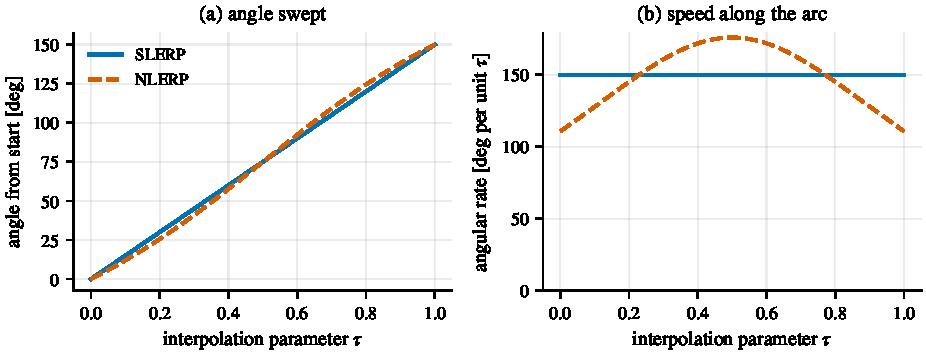
\includegraphics[width=0.84\textwidth]{fig_slerp.pdf}
  \caption{Interpolating between two attitudes $150^\circ$ apart. SLERP sweeps the angle uniformly in the interpolation parameter; normalized linear
  interpolation (NLERP) follows the same path but at a non-uniform speed, fastest in the middle.}
  \label{fig:slerp}
\end{figure}

Ground truth and IMU data rarely share timestamps with images, so attitudes must be interpolated. The correct interpolation follows the
shortest great arc at constant angular velocity: \term{spherical linear interpolation} (SLERP),
\begin{equation}
  q(\tau) = q_0 \qprod \Exp_q\!\big(\tau\,\Log_q(q_0\inv\qprod q_1)\big)
          = \frac{\sin((1 - \tau)\Omega)}{\sin\Omega}\,q_0 + \frac{\sin(\tau\Omega)}{\sin\Omega}\,q_1,
  \qquad \tau\in[0,1],
\end{equation}
with $\cos\Omega = q_0\T q_1$ after flipping the sign of $q_1$ if needed so that $q_0\T q_1 \ge 0$. The first form (using the exponential and
logarithm of \cref{ch:lie}) shows that the relative rotation is applied with a uniformly growing angle; the second is the formula for
interpolating along a great circle of the sphere. Component-wise linear interpolation followed by normalization (NLERP) follows the same
path at a non-uniform speed (\cref{fig:slerp}); it is acceptable only for small angles.

% ==============================================================================
\section{Rigid-body transformations}

A rigid transformation combines a rotation and a translation. Point coordinates transform as
\begin{equation}
  p_w = R_{wb}\,p_b + p_{wb}
  \quad\Longleftrightarrow\quad
  \begin{bmatrix} p_w \\ 1 \end{bmatrix} = \underbrace{\begin{bmatrix} R_{wb} & p_{wb} \\ 0 & 1 \end{bmatrix}}_{T_{wb}}
  \begin{bmatrix} p_b \\ 1 \end{bmatrix}.
\end{equation}
Appending a 1 to the point (\emph{homogeneous coordinates}, developed in \cref{ch:camera}) turns the affine map into a single matrix product.
The $4\times4$ matrices of this form make up the group $\SE$ of rigid motions. Composition and inversion follow from block multiplication:
\begin{equation}
  T_{wc} = T_{wb}T_{bc} = \begin{bmatrix} R_{wb}R_{bc} & R_{wb}p_{bc} + p_{wb} \\ 0 & 1\end{bmatrix},
  \qquad
  T_{wb}\inv = T_{bw} = \begin{bmatrix} R_{wb}\T & -R_{wb}\T p_{wb} \\ 0 & 1 \end{bmatrix}.
  \label{eq:se3-compose}
\end{equation}
The camera pose in the world therefore is $R_{wc} = R_{wb}R_{bc}$ and $p_{wc} = p_{wb} + R_{wb}p_{bc}$, and a world point $p_f$ has camera coordinates
\begin{equation}
  p_c = R_{bc}\T\big(R_{wb}\T(p_f - p_{wb}) - p_{bc}\big),
  \label{eq:world-to-camera}
\end{equation}
which is the first half of the camera measurement model (AGENTS.md C6).

\begin{pitfall}[points versus directions]
Translations apply to points, not to free vectors. A velocity, a gravity vector or a bearing direction transforms with the rotation only,
$v_w = R_{wb}v_b$. In homogeneous coordinates directions carry a $0$ in the fourth component, which drops the translation automatically.
\end{pitfall}

% ==============================================================================
\section{Rotational kinematics}
\label{sec:rot-kinematics}

\subsection{Angular velocity}

Let $R(t) = R_{wb}(t)$ describe a rotating body. Differentiating $R\T R = I$ gives $\dot R\T R + R\T\dot R = 0$, so $R\T\dot R$ is skew-symmetric and
equals $\sx{\omega_b}$ for a unique vector $\omega_b$:
\begin{equation}
  \dot R_{wb} = R_{wb}\,\sx{\omega_b} = \sx{\omega_w}\,R_{wb}, \qquad \omega_w = R_{wb}\,\omega_b ,
  \label{eq:rdot}
\end{equation}
where the second form uses \eqref{eq:skew-rot}. Why is $\omega$ an angular velocity? A point fixed in the body, with constant body coordinates $r_b$,
has world coordinates $r_w = R_{wb}r_b$ and velocity $\dot r_w = \dot R_{wb}r_b = \sx{\omega_w}R_{wb}r_b = \omega_w\times r_w$: every point moves as if the body
were spinning about the axis $\omega_w$ through the origin with angular speed $\|\omega\|$. $\omega_b$ is this angular velocity of $B$ relative to $W$,
expressed in $B$, and it is exactly what a strapdown gyroscope measures (up to bias and noise). The two forms of \eqref{eq:rdot} are the
kinematic origin of the two perturbation conventions of \cref{ch:lie}: a body-frame quantity multiplies on the right, a world-frame quantity on
the left.

\begin{proposition}[Constant body rate]
\label{prop:const-rate}
If $\omega_b$ is constant on $[t_0, t_0 + \Dt]$, then $R(t_0 + \Dt) = R(t_0)\exp(\Dt\sx{\omega_b})$.
\end{proposition}
\begin{proof}
$R(t) = R(t_0)\exp((t - t_0)\sx{\omega_b})$ satisfies \eqref{eq:rdot} by \cref{prop:matexp}, and the solution is unique (\cref{thm:lti-solution}).
\end{proof}

This exact solution is the basis of the multiplicative attitude update used in every integration scheme of \cref{ch:strapdown}. When the
rate varies, the update is still applied step by step with the rate held constant over each short step (\cref{sec:lie-euler}). Note that the
solution is \emph{not} $R(t_0) + \Dt\, R(t_0)\sx{\omega_b}$, which would leave $\SO$.

\subsection{Quaternion kinematics}

The quaternion counterpart of \eqref{eq:rdot} is
\begin{equation}
  \dot q_{wb} = \tfrac12\, q_{wb} \qprod [0,\ \omega_b] = \tfrac12\,\Omega(\omega_b)\,q_{wb},
  \qquad \Omega(\omega) = [\,[0, \omega]\,]_R = \begin{bmatrix} 0 & -\omega\T \\ \omega & -\sx{\omega}\end{bmatrix},
  \label{eq:qdot}
\end{equation}
with constant-rate solution $q(t_0 + \Dt) = q(t_0)\qprod\big[\cos\tfrac{\|\omega\|\Dt}{2},\ \sin\tfrac{\|\omega\|\Dt}{2}\,\tfrac{\omega}{\|\omega\|}\big]$. To derive
\eqref{eq:qdot}, compose $q(t + \dd t) = q(t) \qprod \dd q$, where $\dd q$ is the small body-frame rotation by $\omega_b\,\dd t$. By
\eqref{eq:quat-axis-angle}, $\dd q = [1,\ \tfrac12\omega_b\,\dd t] + O(\dd t^2)$, so $q(t + \dd t) - q(t) = q\qprod[0, \tfrac12\omega_b]\,\dd t$. The factor $\tfrac12$ is
the half angle again.

\subsection{Derivatives in a rotating frame}

Differentiating $v_w = R_{wb}v_b$ with \eqref{eq:rdot} gives the \term{transport theorem}
\begin{equation}
  \dot v_w = R_{wb}\big(\dot v_b + \omega_b \times v_b\big):
  \label{eq:transport}
\end{equation}
the rate of change seen from the fixed frame equals the rate seen in the rotating frame plus the change due to the rotation of the frame itself.
Applying it twice to the position $r$ of a particle relative to a frame rotating with angular velocity $\Omega$ (constant) gives the acceleration
in the fixed (inertial) frame, expressed in rotating coordinates:
\begin{equation}
  a_{\mathrm{inertial}} = \ddot r + 2\,\Omega\times\dot r + \Omega\times(\Omega\times r),
  \label{eq:coriolis}
\end{equation}
where $\ddot r$ and $\dot r$ are the acceleration and velocity seen in the rotating frame. The extra terms are the \term{Coriolis acceleration}
$2\Omega\times\dot r$ and the \term{centripetal acceleration} $\Omega\times(\Omega\times r)$. This formula is the working principle of the vibratory MEMS gyroscope
(\cref{ch:imu}), and it tells us what we neglect by treating the world frame as inertial.

\subsection{The Earth is not an inertial frame}

The world frame $W$ is fixed to the Earth, which rotates at $\Omega_e = 7.292\times10^{-5}$~rad/s. Three effects follow; their sizes justify the
project's simplifications.
\begin{itemize}
  \item \emph{Gyroscopes sense the Earth rate.} $7.3\times10^{-5}$~rad/s is comparable to the bias instability of the EuRoC ADIS16448 and far below its
        noise over short horizons. The project neglects it; its constant body-frame component (while the attitude changes little) is absorbed
        by the gyro bias estimate. High-grade systems model it explicitly and can even find north from it (gyrocompassing).
  \item \emph{Centripetal acceleration.} The term $\Omega_e\times(\Omega_e\times r)$ reaches $0.034~\mathrm{m/s^2}$ at the equator. It is absorbed into the
        local gravity vector: \emph{gravity}, as measured by a plumb line, is gravitation plus this centrifugal term. Its magnitude varies from
        $9.780~\mathrm{m/s^2}$ at the equator to $9.832~\mathrm{m/s^2}$ at the poles; the project uses a constant $9.81$ (AGENTS.md C5), accurate to about
        $10^{-3}$ relative in Zurich, where EuRoC was recorded.
  \item \emph{Coriolis acceleration.} $2\Omega_e\times v$ is about $1.5\times10^{-4}~\mathrm{m/s^2}$ at 1~m/s: below accelerometer noise and bias for a small
        drone, and neglected.
\end{itemize}
Over the minutes and hundreds of meters of a EuRoC sequence, the world frame may therefore be treated as inertial and flat, with constant
gravity.

\begin{takeaways}
\begin{itemize}
  \item $R_{wb}$ maps body coordinates to world coordinates; its columns are the body axes in the world. Adjacent subscripts must match.
  \item Every rotation is an axis-angle rotation, $R = I + \sin\theta\sx{u} + (1-\cos\theta)\sx{u}^2$; $\tr R = 1 + 2\cos\theta$.
  \item Euler angles have intrinsic and extrinsic readings and a singularity at $\pm90^\circ$ pitch; they stay out of the estimator.
  \item Hamilton unit quaternions compose like matrices; $q$ and $-q$ are the same rotation; the quaternion of a rotation by $\theta$ uses $\theta/2$.
  \item Eigen's constructor is $w$-first, its storage $w$-last, EuRoC is $w$-first. JPL formulas must be re-derived, not copied.
  \item $\dot R_{wb} = R_{wb}\sx{\omega_b}$; with constant $\omega_b$ the update $R \leftarrow R\exp(\Dt\sx{\omega_b})$ is exact.
  \item Derivatives in rotating frames pick up $\omega\times$ terms; for a small drone over minutes, the Earth's rotation is negligible.
\end{itemize}
\end{takeaways}

\begin{exercises}
  \item Show that the columns of any $R \in \SO$ are orthonormal and that $\det R = +1$ implies the third column is the cross product of the first two.
  \item Verify $R_x(90^\circ)R_y(90^\circ) \neq R_y(90^\circ)R_x(90^\circ)$ by computing both products, and describe each rotation physically.
  \item Derive \eqref{eq:euler-rates} from \eqref{eq:zyx} and $\sx{\omega_b} = R\T\dot R$.
  \item Convert the rotation of the worked example ($120^\circ$ about $(1,1,1)/\sqrt3$) to ZYX Euler angles.
  \item Prove that $[p]_L[q]_R = [q]_R[p]_L$. What does this say about associativity of the quaternion product?
  \item Show that $R(-q) = R(q)$ and compute the quaternion of a $270^\circ$ rotation about $z$ in its canonical form ($w \ge 0$). What rotation angle and
        axis does the canonical form describe?
  \item Implement Shepperd's method and test it on rotations by $0^\circ$, $90^\circ$, $179.9999^\circ$ and $180^\circ$.
  \item Write a function that converts a EuRoC ground-truth row into $p_{wb}$, $q_{wb}$, $v_{wb}$, $b_g$ and $b_a$. Design a fixture row whose values would
        expose a swapped $w/z$ and swapped biases.
  \item Given $T_{bc}$ from \code{cam0/sensor.yaml} (\cref{app:euroc}), compute the camera's optical axis in body coordinates.
  \item Show that if $\omega_b$ varies in time, $R(t) = R(0)\exp\big(\int_0^t\sx{\omega_b}\,\dd s\big)$ is in general \emph{wrong}. Construct a counterexample with
        piecewise-constant rates.
  \item Derive \eqref{eq:coriolis} by applying \eqref{eq:transport} twice.
\end{exercises}
% Solutions to the exercises of Chapter 7.
\begin{solutions}
  \item Write $R = [r_1\ r_2\ r_3]$. The entry $(i, j)$ of $R\T R = I$ is $r_i\T r_j = \delta_{ij}$: the columns are orthonormal. The unit vectors orthogonal
        to both $r_1$ and $r_2$ are exactly $\pm r_1\times r_2$ (a unit vector, by Lagrange's identity), so $r_3 = \pm r_1\times r_2$. The determinant is the
        triple product $\det R = r_3\T(r_1\times r_2) = \pm\|r_1\times r_2\|^2 = \pm1$, so $\det R = +1$ selects $r_3 = r_1\times r_2$: the body axes form a
        right-handed frame.

  \item From the elementary matrices,
        \[
          R_x(90^\circ)R_y(90^\circ) = \begin{bmatrix}0 & 0 & 1\\ 1 & 0 & 0\\ 0 & 1 & 0\end{bmatrix}, \qquad
          R_y(90^\circ)R_x(90^\circ) = \begin{bmatrix}0 & 1 & 0\\ 0 & 0 & -1\\ -1 & 0 & 0\end{bmatrix}.
        \]
        The first sends $e_x \to e_y$, $e_y \to e_z$, $e_z \to e_x$ (its columns): it cycles the axes, a $120^\circ$ rotation about $(1,1,1)/\sqrt3$. The
        second has trace 0 (angle $120^\circ$) and $(R - R\T)\veeop = (1, 1, -1)$, so it is a $120^\circ$ rotation about $(1, 1, -1)/\sqrt3$. Physically, read
        as intrinsic sequences: the first turns a book $90^\circ$ about its $x$-axis and then $90^\circ$ about its new $y$-axis; the second does the two
        quarter turns in the other order and leaves the book in a different orientation.

  \item Write $R = R_zR_yR_x$ with $\dot R_z = \dot\psi R_z\sx{e_z}$, $\dot R_y = \dot\vartheta R_y\sx{e_y}$, $\dot R_x = \dot\varphi R_x\sx{e_x}$. Then
        \[
          R\T\dot R = \dot\psi\,R_x\T R_y\T\sx{e_z}R_yR_x + \dot\vartheta\,R_x\T\sx{e_y}R_x + \dot\varphi\,\sx{e_x}
          = \big[\dot\psi\,R_x\T R_y\T e_z + \dot\vartheta\,R_x\T e_y + \dot\varphi\,e_x\big]_\times
        \]
        by \eqref{eq:skew-rot}. With $R_y\T e_z = (-s_\vartheta, 0, c_\vartheta)$, $R_x\T(-s_\vartheta, 0, c_\vartheta) = (-s_\vartheta, s_\varphi c_\vartheta, c_\varphi c_\vartheta)$ and
        $R_x\T e_y = (0, c_\varphi, -s_\varphi)$,
        \[
          \omega_b = \begin{bmatrix} 1 & 0 & -s_\vartheta \\ 0 & c_\varphi & s_\varphi c_\vartheta \\ 0 & -s_\varphi & c_\varphi c_\vartheta \end{bmatrix}
                     \begin{bmatrix}\dot\varphi\\ \dot\vartheta\\ \dot\psi\end{bmatrix}.
        \]
        The matrix has determinant $c_\vartheta$. Solving the last two rows gives $\dot\vartheta = c_\varphi\omega_y - s_\varphi\omega_z$ and
        $\dot\psi = (s_\varphi\omega_y + c_\varphi\omega_z)/c_\vartheta$, and the first row gives $\dot\varphi = \omega_x + s_\vartheta\dot\psi$, which is \eqref{eq:euler-rates}.
        The determinant $c_\vartheta$ vanishes at $\vartheta = \pm90^\circ$: gimbal lock.

  \item The rotation is the axis-cycling matrix of Exercise 7.2, $R = \begin{bmatrix}0 & 0 & 1\\ 1 & 0 & 0\\ 0 & 1 & 0\end{bmatrix}$. With the conversion formulas,
        $\vartheta = \atantwo(-R_{31}, \sqrt{R_{11}^2 + R_{21}^2}) = \atantwo(0, 1) = 0$, $\varphi = \atantwo(R_{32}, R_{33}) = \atantwo(1, 0) = 90^\circ$ and
        $\psi = \atantwo(R_{21}, R_{11}) = \atantwo(1, 0) = 90^\circ$: yaw $90^\circ$, pitch $0$, roll $90^\circ$. Check: $R_z(90^\circ)R_x(90^\circ)$ reproduces $R$, as the worked
        example $q_z\qprod q_x$ already showed.

  \item Apply both sides to an arbitrary quaternion $r$. By definition $[q]_Rr = r\qprod q$ and $[p]_Lr = p\qprod r$, so
        \[
          [p]_L[q]_R\,r = p\qprod(r\qprod q), \qquad [q]_R[p]_L\,r = (p\qprod r)\qprod q .
        \]
        The two agree for every $r$ exactly because the Hamilton product is associative, so the matrices are equal. (Multiplying out the blocks and
        using $\sx{a}\sx{b} = ba\T - (a\T b)I$ confirms it directly.) Conversely, the identity $[p]_L[q]_R = [q]_R[p]_L$ for all $p, q$ \emph{is} the
        statement of associativity: multiplying on the left and on the right are commuting operations.

  \item $R(q)$ in \eqref{eq:quat-to-rot} is a homogeneous quadratic in the components of $q$, so $R(-q) = (-1)^2R(q) = R(q)$. A $270^\circ$ rotation about
        $z$ has
        \[
          q = \big[\cos135^\circ,\ \sin135^\circ e_z\big] = \big[-\tfrac{\sqrt2}{2},\ (0, 0, \tfrac{\sqrt2}{2})\big].
        \]
        Its scalar part is negative, so the canonical form is $-q = [\tfrac{\sqrt2}{2},\ (0, 0, -\tfrac{\sqrt2}{2})]$. It describes a rotation by
        $2\arccos(\tfrac{\sqrt2}2) = 90^\circ$ about $-e_z$: the same rotation as $270^\circ$ about $+e_z$, reached the short way round. Canonicalization
        always yields an angle in $[0, \pi]$.

  \item A direct implementation picks the largest of the four squared components, computed from the diagonal:
\begin{lstlisting}[style=py]
def shepperd(R):
    t = np.trace(R)
    c = [1 + t, 1 + R[0,0] - R[1,1] - R[2,2], 1 - R[0,0] + R[1,1] - R[2,2], 1 - R[0,0] - R[1,1] + R[2,2]]
    i = int(np.argmax(c)); s = 2 * np.sqrt(c[i])          # s = 4 * (largest component)
    a, b, d = R[2,1] - R[1,2], R[0,2] - R[2,0], R[1,0] - R[0,1]   # 4wx, 4wy, 4wz
    e, f, g = R[0,1] + R[1,0], R[0,2] + R[2,0], R[1,2] + R[2,1]   # 4xy, 4xz, 4yz
    q = [[s/4, a/s, b/s, d/s], [a/s, s/4, e/s, f/s], [b/s, e/s, s/4, g/s], [d/s, f/s, g/s, s/4]][i]
    return np.array(q) if q[0] >= 0 else -np.array(q)
\end{lstlisting}
        Testing against the quaternion used to build each matrix (axis $(1, -2, 0.5)/\|\cdot\|$) gives errors of $0$, $3\times10^{-16}$, $2\times10^{-18}$ and
        $10^{-16}$ at $0^\circ$, $90^\circ$, $179.9999^\circ$ and $180^\circ$. The naive formula $w = \tfrac12\sqrt{1 + \tr R}$, $v = (R - R\T)\veeop/4w$ is exact at the first two,
        wrong by $9\times10^{-6}$ at $179.9999^\circ$ (it divides by $w \approx 9\times10^{-7}$, computed from the difference $1 + \tr R \approx 3\times10^{-12}$), and
        undefined at $180^\circ$.

  \item The ground-truth row is \code{timestamp, p\_x, p\_y, p\_z, q\_w, q\_x, q\_y, q\_z, v\_x, v\_y, v\_z, bw\_x, bw\_y, bw\_z, ba\_x, ba\_y, ba\_z} (AGENTS.md C7).
        In C++ the parser constructs each piece explicitly:
\begin{lstlisting}
p_wb = Eigen::Vector3d(r[1], r[2], r[3]);
q_wb = Eigen::Quaterniond(r[4], r[5], r[6], r[7]).normalized();  // w first
v_wb = Eigen::Vector3d(r[8], r[9], r[10]);
b_g  = Eigen::Vector3d(r[11], r[12], r[13]);   // gyro bias comes first
b_a  = Eigen::Vector3d(r[14], r[15], r[16]);
\end{lstlisting}
        A good fixture row makes every plausible mistake produce a detectably different result: all quaternion components distinct and of
        different signs, e.g.\ $q = (w, x, y, z) = (0.8, 0.2, -0.4, 0.4)$ (unit norm), so that reading it as $[x, y, z, w]$ gives a different rotation;
        biases of different magnitudes and signs, e.g.\ $b_g = (0.01, 0.02, 0.03)$ and $b_a = (-0.1, -0.2, -0.3)$, so that swapping them is visible;
        and position and velocity that differ in every component. The test asserts each field and also checks that $R(q)\,e_x$ equals the column
        computed by hand, which catches a wrong constructor order even when the norm is unchanged. A row with the identity quaternion, or with
        equal biases, would let all these bugs pass.

  \item The optical axis is the camera's $z$-axis; in body coordinates it is $R_{bc}e_z$, the third column of the rotation block of $T_{bc}$. With the
        values of \cref{app:euroc} it is $(0.0041, 0.0257, 0.9997)$: the camera looks along the body $+z$-axis, tilted by $\arccos(0.9997) = 1.5^\circ$. The
        other columns show the camera $x$-axis along body $+y$ and the camera $y$-axis along body $-x$; since the EuRoC IMU's $x$-axis points up at
        rest, the image $y$-axis (rows, increasing downwards) indeed points down.

  \item By \cref{prop:stm} the formula holds only if the matrices $\sx{\omega_b(t)}$ commute for all $t$, i.e.\ if $\omega_b(t)$ keeps a fixed direction. Counterexample:
        $\omega_b = (\pi/2, 0, 0)$ on $[0, 1)$ and $(0, \pi/2, 0)$ on $[1, 2)$. By \cref{prop:const-rate} applied to each segment the true attitude is
        $R(2) = R(0)R_x(90^\circ)R_y(90^\circ)$, a $120^\circ$ rotation relative to $R(0)$ (Exercise 7.2). The formula gives
        $R(0)\exp(\sx{(\pi/2, \pi/2, 0)})$, a $127^\circ$ rotation about $(1, 1, 0)/\sqrt2$, which is wrong by $1.1$~rad. This is the coning error in its
        crudest form (\cref{sec:coning}).

  \item Let $r_I = Rr$ be the particle's position in inertial coordinates, with $\dot R = R\sx{\Omega}$ and $\Omega$ constant. The transport theorem gives
        $\dot r_I = R(\dot r + \Omega\times r) = Ru$ with $u = \dot r + \Omega\times r$. Applying it again to $u$,
        \[
          \ddot r_I = R(\dot u + \Omega\times u) = R\big(\ddot r + \Omega\times\dot r + \Omega\times\dot r + \Omega\times(\Omega\times r)\big),
        \]
        using $\dot\Omega = 0$. Expressed in rotating coordinates ($R\T\ddot r_I$), the inertial acceleration is
        $\ddot r + 2\,\Omega\times\dot r + \Omega\times(\Omega\times r)$, which is \eqref{eq:coriolis}. The factor 2 comes from the two applications, each contributing
        one $\Omega\times\dot r$.
\end{solutions}


\chapter{Lie Theory for Rotations}
\label{ch:lie}

\begin{objectives}
\begin{itemize}
  \item Understand $\SO$ as a curved manifold with a flat tangent space, and why an estimator needs both.
  \item Use the exponential and logarithm maps, in matrix and quaternion form, and implement them robustly.
  \item Distinguish local (right) and global (left) perturbations, and move perturbations across a
        rotation with the adjoint.
  \item Define Jacobians of functions of rotations, derive the right Jacobian $\Jr$, and build a table
        of elementary Jacobians from which every Jacobian in the project can be assembled.
  \item Represent and propagate uncertainty on $\SO$, and test manifold Jacobians numerically.
\end{itemize}
\end{objectives}

This chapter is the mathematical core of the notes. Its conclusions fit in a few lines (the
$\bplus$/$\bminus$ operators of \cref{sec:boxplus} and the Jacobian table of \cref{tab:jacobians}),
but the reasoning behind them is what lets you derive any new Jacobian correctly. The treatment
follows the ``micro Lie theory'' of Solà et al.~\cite{sola2018micro}, specialized to $\SO$ with the
conventions of this project. Barfoot~\cite{barfoot2017state} covers the same material in greater depth.

% ------------------------------------------------------------------------------
\section{Why estimation needs Lie theory}

A Kalman filter represents uncertainty as a mean and a covariance and corrects the mean by adding
a vector. Both operations assume the state lives in a vector space. Attitude does not.
\begin{itemize}
  \item \textbf{Addition leaves the space.} If $\hat q$ is a unit quaternion and $\delta q$ a small
        4-vector, $\hat q + \delta q$ is generally not unit length. The same holds for rotation matrices.
  \item \textbf{Redundant parameters give singular covariances.} A unit quaternion has four
        components but three degrees of freedom. A $4\times4$ covariance of a unit quaternion must be
        singular along the radial direction, and keeping it exactly singular under rounding is hopeless.
  \item \textbf{Minimal parameters have singularities.} Euler angles (\cref{ch:rotations}) are minimal
        but singular at gimbal lock.
\end{itemize}

\begin{keyidea}[the Earth and its tangent planes]
The surface of the Earth is curved, yet a town map drawn on flat paper is perfectly accurate for a
walk across town. The map is the \emph{tangent plane} at your location. It works as long as you do
not walk too far, and when you move to a new town you draw a new map. An estimator does the same:
it stores the attitude on the curved space $\SO$ (the globe), and expresses small uncertainties and
corrections in the flat 3D tangent space at the current estimate (the town map). The exponential
map turns a step on the map into a point on the globe, and the logarithm map does the reverse.
\end{keyidea}

% ------------------------------------------------------------------------------
\section{Warm-up: rotations of the plane}
\label{sec:so2}

Every idea of this chapter appears, in its simplest form, for planar rotations $R(\theta)$. Work through them here; the rest of the chapter
asks only what changes in three dimensions.
\begin{itemize}
  \item \emph{The set.} Planar rotations form a circle: $R(\theta)$ and $R(\theta + 2\pi)$ are the same. The set is one-dimensional but curved, and it is
        not a vector space ($R(\alpha) + R(\beta)$ is not a rotation).
  \item \emph{The tangent space.} Differentiating $R(\theta)$ at $\theta = 0$ gives $\frac{\dd R}{\dd\theta}(0) = \begin{bmatrix}0 & -1\\ 1 & 0\end{bmatrix}$; every velocity at the
        identity is a multiple of this skew-symmetric matrix. The tangent space is a line, coordinatized by a single number.
  \item \emph{Exponential and logarithm.} $\exp\big(\theta\begin{bmatrix}0 & -1\\ 1 & 0\end{bmatrix}\big) = R(\theta)$ (sum the series, or solve
        $\dot R = R\begin{bmatrix}0&-1\\1&0\end{bmatrix}$), so ``$\Exp$'' maps an angle to a rotation. Its inverse ``$\Log$'' recovers the angle,
        $\theta = \atantwo(R_{21}, R_{11}) \in (-\pi, \pi]$, unique only up to the choice of branch.
  \item \emph{Perturbations.} An estimate $R(\hat\theta)$ with a small error is $R(\hat\theta)R(\delta\theta) = R(\hat\theta + \delta\theta)$. Because planar rotations commute,
        perturbing on the left or on the right is the same, and the error of the composition is just the sum of the angles.
  \item \emph{Jacobians.} The derivative of $\Exp$ is the identity (1), and nothing like the right Jacobian appears.
\end{itemize}
In the plane, therefore, one can simply estimate the angle as a scalar, as long as differences are wrapped to $(-\pi, \pi]$. In three dimensions
rotations do not commute, the identity $R(\alpha)R(\beta) = R(\alpha + \beta)$ fails for rotation vectors with different axes, and left and right
perturbations differ. Each of these failures produces a new object in this chapter: the adjoint, the Baker--Campbell--Hausdorff formula, and the
right and left Jacobians.

% ------------------------------------------------------------------------------
\section{Manifolds, groups and Lie groups}

\subsection{Manifolds and tangent spaces}

\index{manifold}
A smooth $n$-dimensional \term{manifold} is a space that looks like $\R^n$ near every point. Precisely, each point has a neighborhood that can be
mapped smoothly and invertibly onto an open set of $\R^n$ (a \emph{chart}), and where two charts overlap, the change of coordinates between them is
smooth. The surface of a sphere is a 2D manifold: latitude and longitude form a chart away from the poles, and a second chart covers the poles. A
manifold usually needs several charts; a single chart for the whole sphere does not exist, and neither does one for $\SO$, which is why every
three-number parameterization of attitude has singularities.

A \term{tangent vector} at a point $x$ of a manifold is the velocity $\dot\gamma(0)$ of a smooth curve $\gamma(t)$ through $\gamma(0) = x$. The tangent vectors
at $x$ form a vector space, the \term{tangent space} $T_x\mathcal M$, of the same dimension as the manifold. For a manifold that sits inside a larger
vector space (as $\SO$ sits inside $\R^{3\times3}$), tangent vectors are ordinary vectors tangent to the surface: the tangent plane of a sphere
in the Earth analogy.

\subsection{Groups}

\begin{definition}[Group]
\index{group}
A \term{group} $(\mathcal{G}, \circ)$ is a set with an operation $\circ$ that is associative, has an identity element $\mathcal{E}$
($\mathcal{E}\circ\mathcal{X} = \mathcal{X}\circ\mathcal{E} = \mathcal{X}$), and an inverse $\mathcal{X}\inv$ for every element
($\mathcal{X}\circ\mathcal{X}\inv = \mathcal{E}$).
\end{definition}

Commutativity is \emph{not} required. Examples: $(\R^n, +)$ (identity $0$, inverse $-x$); the invertible $n\times n$ matrices under multiplication;
$\SO$; the unit quaternions under the Hamilton product; the rigid motions $\SE$. A group can also \emph{act} on another set: a rotation acts on
vectors by $v \mapsto Rv$, and a rigid motion acts on points by $p \mapsto Rp + t$. These actions are how groups enter measurement models.

\begin{definition}[Lie group]
\index{Lie group}
A \term{Lie group} is a group that is also a smooth manifold, such that composition and inversion are smooth maps. A \emph{matrix Lie group} is a
Lie group whose elements are invertible matrices and whose operation is matrix multiplication.
\end{definition}

Being a group as well gives a Lie group a remarkable property. Multiplication by a fixed element maps a neighborhood of the identity smoothly onto
a neighborhood of that element: the space looks the same everywhere. All local calculus can therefore be done once, at the identity, and
carried to any other element by composition. This is what makes estimation on $\SO$ tractable: one tangent space (at the identity), one
exponential map, and one set of Jacobian formulas serve every attitude.

\begin{center}\small
\begin{tabular}{@{}l l l l@{}}
\toprule
Group & Elements & Dimension & Role in VIO \\
\midrule
$(\R^n, +)$ & vectors & $n$ & position, velocity, biases \\
$\mathrm{SO}(2)$ & planar rotations & 1 & toy examples \\
$\SO$ & $3\times3$ rotation matrices & 3 & attitude \\
$S^3$ & unit quaternions & 3 & attitude (double cover of $\SO$) \\
$\SE$ & rigid transformations & 6 & poses, extrinsics \\
\bottomrule
\end{tabular}
\end{center}

% ------------------------------------------------------------------------------
\section{The Lie algebra and tangent spaces}

Consider a smooth curve $R(t) \in \SO$ with $R(0) = I$. Differentiating $R\T R = I$ at $t = 0$ gives
$\dot R(0)\T + \dot R(0) = 0$: the velocity at the identity is skew-symmetric. The set of all such
velocities is the \emph{Lie algebra}
\begin{equation}
  \so = \{\, \Omega \in \R^{3\times3} : \Omega\T = -\Omega \,\} = \{\, \sx{\phi} : \phi \in \R^3 \,\},
\end{equation}
a three-dimensional vector space identified with $\R^3$ by the hat and vee maps,
$\phi\hatop = \sx{\phi}$ and $\sx{\phi}\veeop = \phi$. Unlike $\SO$ itself, the Lie algebra is flat:
we can add its elements, scale them, and put Gaussian distributions on them.

\index{Lie bracket}
The Lie algebra carries one more operation, the \emph{Lie bracket} (commutator) $[X, Y] = XY - YX$, which measures how much two infinitesimal
motions fail to commute. The commutator of two skew-symmetric matrices is skew-symmetric, and by \eqref{eq:skew-commutator}
\begin{equation}
  \big[\sx{a}, \sx{b}\big] = \sx{a \times b} .
\end{equation}
So $\so$ with its bracket is $\R^3$ with the cross product. The cross product, which is zero only for parallel vectors, is the infinitesimal
version of the non-commutativity of rotations: rotations about parallel axes commute, all others do not.

At a general point $R$, the tangent space consists of the velocities of curves through $R$. From
\eqref{eq:rdot}, every such velocity can be written in two ways,
\begin{equation}
  \dot R = R\,\sx{\omega_b} = \sx{\omega_w}\,R, \qquad \omega_w = R\,\omega_b,
\end{equation}
so the tangent space at $R$ can be identified with $\R^3$ in two ways: by a vector expressed in the
\emph{local} (body) frame, multiplying on the right, or by a vector expressed in the \emph{global}
(world) frame, multiplying on the left. This is the origin of the two perturbation conventions of
\cref{sec:perturbations}. The project uses the local one.

\begin{figure}[t]
\centering
\begin{tikzpicture}[scale=1.0]
  % manifold surface
  \shade[top color=white, bottom color=primary!22] (0,0) ellipse (4.4 and 2.4);
  \draw[primary, thick] (0,0) ellipse (4.4 and 2.4);
  \draw[primary!50, dashed] (-4.4,0) arc (180:360:4.4 and 0.8);
  \node[primary, font=\small] at (-3.0,-1.5) {$\SO$};
  % tangent plane at Rhat
  \coordinate (X) at (-0.9,2.0);
  \fill[white, opacity=0.85, draw=black!55] ($(X)+(-2.4,0.35)$) -- ($(X)+(3.0,0.85)$) -- ($(X)+(3.6,-0.15)$) -- ($(X)+(-1.8,-0.65)$) -- cycle;
  \node[font=\small, anchor=west] at ($(X)+(-2.25,0.25)$) {$T_{\hat R}\SO \cong \R^3$};
  \fill[black] (X) circle (1.8pt) node[below=2pt] {$\hat R$};
  % the tangent vector
  \coordinate (V) at ($(X)+(2.4,0.3)$);
  \draw[->, very thick, plotorange] (X) -- (V) node[above=1pt, font=\small] {$\delta\theta$};
  % point on the manifold
  \coordinate (Y) at (2.4,0.9);
  \fill[plotgreen] (Y) circle (1.8pt);
  \node[plotgreen!70!black, below right=1pt, font=\small, fill=white, fill opacity=0.85, text opacity=1, inner sep=1.5pt, rounded corners=1pt] at (Y) {$\hat R\,\Exp(\delta\theta)$};
  \draw[->, plotgreen, thick, dashed] ($(V)+(0.05,-0.08)$) to[bend left=30] node[right=1pt, font=\footnotesize, pos=0.6] {$\Exp$} ($(Y)+(0.02,0.08)$);
  % logarithm back to the tangent space
  \draw[->, plotpurple, thick] ($(Y)+(-0.1,-0.05)$) to[bend left=25] node[below=1pt, font=\footnotesize] {$\Log(\hat R\T\,\cdot\,)$} ($(X)+(0.05,-0.12)$);
\end{tikzpicture}
\caption{The manifold $\SO$ and its tangent space at the estimate $\hat R$. A small error or correction
$\delta\theta \in \R^3$ lives in the flat tangent space. The exponential map wraps it onto the manifold as
$\hat R\Exp(\delta\theta)$, and the logarithm recovers it.}
\label{fig:tangent-space}
\end{figure}

% ------------------------------------------------------------------------------
\section{The exponential map}

\begin{definition}[Exponential map of $\SO$]
$\exp: \so \to \SO$ is the matrix exponential. Composed with the hat map it gives the
\emph{capitalized} exponential
\begin{equation}
  \Exp: \R^3 \to \SO, \qquad \Exp(\phi) = \exp(\sx{\phi}).
\end{equation}
By Rodrigues' formula (\cref{thm:rodrigues}), with $\theta = \|\phi\|$,
\begin{equation}
  \Exp(\phi) = I + \frac{\sin\theta}{\theta}\,\sx{\phi} + \frac{1 - \cos\theta}{\theta^2}\,\sx{\phi}^2 .
  \label{eq:Exp}
\end{equation}
\end{definition}

$\Exp(\phi)$ is the rotation by angle $\|\phi\|$ about the axis $\phi/\|\phi\|$. Its main properties are
$\Exp(0) = I$, $\Exp(-\phi) = \Exp(\phi)\T$, and $\Exp(s\phi)\Exp(t\phi) = \Exp((s+t)\phi)$: rotations about a
\emph{common} axis compose by adding angles. $\Exp$ is onto $\SO$, and one-to-one on the open ball
$\|\phi\| < \pi$.

\paragraph{Why the exponential?} The curve $R(t) = \Exp(t\phi)$ is the motion of a body spinning at the constant body rate $\phi$: it solves
$\dot R = R\sx{\phi}$ with $R(0) = I$ (\cref{prop:const-rate}), and it is a \emph{one-parameter subgroup}, $R(s)R(t) = R(s + t)$. The exponential
map thus sends each tangent vector at the identity to the point reached by moving ``straight'' in that direction for unit time. In every Lie
group, the exponential is defined the same way, which is why the same machinery works for $\SO$, $\SE$ and the extended poses used by
invariant filters.

\paragraph{Quaternion exponential.} The unit quaternion corresponding to $\Exp(\phi)$ follows from
\eqref{eq:quat-axis-angle}:
\begin{equation}
  \Exp_q(\phi) = \begin{bmatrix} \cos(\theta/2) \\ \dfrac{\sin(\theta/2)}{\theta}\,\phi \end{bmatrix},
  \qquad R\big(\Exp_q(\phi)\big) = \Exp(\phi).
  \label{eq:Expq}
\end{equation}
This is the quaternion exponential of the pure quaternion $[0, \phi/2]$; the half angle is the double
cover again. Since $\Exp_q(\phi)$ has $w = \cos(\theta/2) \ge 0$ for $\theta \le \pi$, its output is
already in canonical form on that range.

\subsection{Numerical evaluation and the Taylor branches}
\label{sec:taylor}

Formulas \eqref{eq:Exp} and \eqref{eq:Expq}, and the Jacobian formulas later in this chapter, are built
from a handful of scalar \emph{coefficient functions} of $\theta$:
\begin{equation}
  A(\theta) = \frac{\sin\theta}{\theta},\quad
  B(\theta) = \frac{1-\cos\theta}{\theta^2},\quad
  C(\theta) = \frac{\theta - \sin\theta}{\theta^3},\quad
  D(\theta) = \frac{1}{\theta^2} - \frac{\cot(\theta/2)}{2\theta}.
\end{equation}
All four are smooth, even functions with finite limits at $\theta = 0$, but their formulas read $0/0$
there. Their Taylor series are
\begin{equation}
\begin{aligned}
  A &= 1 - \tfrac{\theta^2}{6} + \tfrac{\theta^4}{120} - \cdots, &
  B &= \tfrac12 - \tfrac{\theta^2}{24} + \tfrac{\theta^4}{720} - \cdots, \\
  C &= \tfrac16 - \tfrac{\theta^2}{120} + \tfrac{\theta^4}{5040} - \cdots, &
  D &= \tfrac1{12} + \tfrac{\theta^2}{720} + \tfrac{\theta^4}{30240} + \cdots,
\end{aligned}
\label{eq:coeff-taylor}
\end{equation}
and for the quaternion map
$\cos\frac\theta2 = 1 - \frac{\theta^2}{8} + \frac{\theta^4}{384} - \cdots$ and
$\frac{\sin(\theta/2)}{\theta} = \frac12 - \frac{\theta^2}{48} + \frac{\theta^4}{3840} - \cdots$.

There are two distinct numerical issues.
\begin{enumerate}
  \item \textbf{Division by zero.} At $\theta = 0$ exactly (a perfectly still IMU, or a zero
        correction), every formula evaluates to \code{NaN}, and a single \code{NaN} propagates through
        $P$ and destroys the filter. For tiny $\theta$, $\theta^2$ can also underflow to zero.
  \item \textbf{Cancellation.} $B$, $C$ and $D$ subtract nearly equal quantities. As
        \cref{fig:taylor}(a) shows, their naive evaluation has relative error of order $u/\theta^2$:
        about $10^{-8}$ at $\theta = 10^{-4}$, and complete loss below $\theta \approx 10^{-8}$.
        $A$ and the quaternion coefficients involve no subtraction and are accurate everywhere except at
        $0/0$.
\end{enumerate}

\begin{figure}[t]
  \centering
  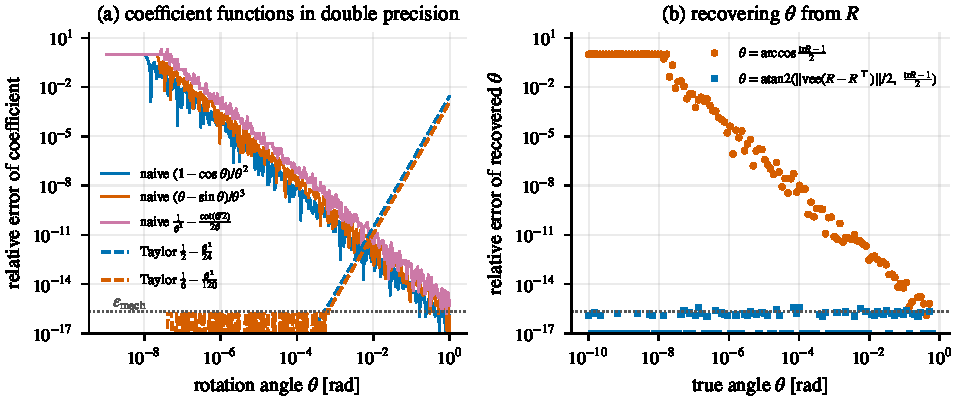
\includegraphics[width=\textwidth]{fig_taylor.pdf}
  \caption{(a) Relative error of the coefficient functions evaluated naively in double precision
  (solid) and with a two-term Taylor series (dashed), against a 60-digit reference. The naive error
  grows like $u/\theta^2$ as $\theta\to0$, and the truncation error of the series grows like $\theta^4$.
  (b) Recovering the angle from a rotation matrix: $\arccos$ loses accuracy like $u/\theta^2$ and
  returns exactly zero below $10^{-8}$, while the $\atantwo$ form is accurate to machine precision at
  every angle.}
  \label{fig:taylor}
\end{figure}

How much does the cancellation matter? It depends on what the coefficient multiplies. A coefficient
with absolute error $\epsilon_c$ that multiplies $\sx{\phi}^k$ contributes an error of about
$\epsilon_c\theta^k$ to the matrix. For $B$, $C$ and $D$, $\epsilon_c \approx u/\theta^2$, so:
\begin{center}\small
\begin{tabular}{@{}l l c l@{}}
\toprule
Function & cancelling coefficient & multiplies & naive absolute error \\
\midrule
$\Exp(\phi)$ & $B$ & $\sx{\phi}^2$ & $\approx u$ \quad (harmless) \\
$\Jr(\phi)$ & $B$ & $\sx{\phi}$ & $\approx u/\theta$ \quad (\textbf{harmful}: $3\times10^{-9}$ at $\theta = 10^{-8}$) \\
$\Jr(\phi)$ & $C$ & $\sx{\phi}^2$ & $\approx u$ \\
$\Jrinv(\phi)$ & $D$ & $\sx{\phi}^2$ & $\approx u$ \\
\bottomrule
\end{tabular}
\end{center}

\begin{keyidea}[why the Taylor branch exists, and how to choose its threshold]
Every function needs a guard against $0/0$. Beyond that, the branch matters for accuracy wherever a
cancelling coefficient multiplies a low power of $\sx{\phi}$, as in $\Jr$. To choose the threshold
$\theta_0$ and the number of terms, balance the two error curves of \cref{fig:taylor}(a): keeping terms
through $\theta^{2m}$ leaves a truncation error of order $\theta^{2m+2}$, and the exact formula has a
rounding error of order $u/\theta^2$. Below the crossing point use the series, above it the formula.
For two-term series ($m = 1$) the curves cross near $\theta \approx 3\times10^{-3}$, where both relative
errors are about $10^{-12}$; adding the $\theta^4$ term moves the crossing to larger angles and lowers
the error there. Remember to multiply by $\theta^k$ when translating a coefficient error into a matrix
error. Record the choice and this justification next to the code (Milestone 2).
\end{keyidea}

% ------------------------------------------------------------------------------
\section{The logarithm map}
\label{sec:log}

\begin{definition}[Logarithm map]
$\Log: \SO \to \R^3$ returns the rotation vector $\phi$ with $\|\phi\| \le \pi$ such that
$\Exp(\phi) = R$.
\end{definition}

For angles strictly between $0$ and $\pi$ the answer is unique. Combining the two equations of
\eqref{eq:trace-angle},
\begin{equation}
  \theta = \atantwo\!\Big( \tfrac12\big\|(R - R\T)\veeop\big\|,\ \tfrac12(\tr R - 1) \Big), \qquad
  \Log(R) = \frac{\theta}{2\sin\theta}\,(R - R\T)\veeop .
  \label{eq:Log}
\end{equation}
The $\atantwo$ form is essential. The common textbook formula $\theta = \arccos\big((\tr R - 1)/2\big)$ is
correct mathematically but numerically unstable near $\theta = 0$, where $\arccos$ has infinite slope,
and loses half the significant digits (\cref{fig:taylor}b). Three regimes need care in code.

\begin{enumerate}
  \item \textbf{Small angles.} $\theta/(2\sin\theta) \to \tfrac12$, so use
        $\Log(R) \approx \tfrac12(1 + \tfrac{\theta^2}{6})(R - R\T)\veeop$.
  \item \textbf{Generic angles.} Use \eqref{eq:Log} directly.
  \item \textbf{Angles near $\pi$.} $\sin\theta \to 0$ and $(R - R\T)\veeop = 2\sin\theta\,u$ vanishes, so
        the axis cannot be recovered from the skew-symmetric part. Use the symmetric part instead: from
        \eqref{eq:rodrigues}, $\tfrac12(R + R\T) = \cos\theta\,I + (1-\cos\theta)\,uu\T$, so
        $uu\T = \big(\tfrac12(R + R\T) - \cos\theta\, I\big)/(1 - \cos\theta)$. Take the column with the largest
        diagonal entry, normalize it to get $\pm u$, and fix the sign so that $u\T(R - R\T)\veeop \ge 0$.
\end{enumerate}

\begin{figure}[t]
\centering
\begin{tikzpicture}[scale=1.0]
  \fill[primarylight] (0,0) circle (2.0);
  \draw[primary, thick] (0,0) circle (2.0);
  \fill (0,0) circle (1.4pt) node[below right] {$I$};
  \draw[->, thick, plotorange] (0,0) -- (1.2,0.8) node[above right=-2pt] {$\phi$};
  \fill[plotgreen] (40:2.0) circle (2pt) node[above right] {$\pi u$};
  \fill[plotgreen] (220:2.0) circle (2pt) node[below left] {$-\pi u$};
  \draw[plotgreen, dashed, <->] (40:1.9) -- (220:1.9);
  \draw[->, plotpurple, thick] (-0.3,-1.2) .. controls (0.6,-1.4) and (1.4,-1.5) .. (330:2.0);
  \draw[->, plotpurple, thick] (150:2.0) .. controls (-1.2,0.6) .. (-0.6,0.4);
  \node[plotpurple, font=\footnotesize, align=left] at (3.6,-1.1) {a path leaving the ball\\re-enters at the\\antipodal point};
  \node[primary, font=\footnotesize] at (0,2.35) {$\|\phi\| \le \pi$};
\end{tikzpicture}
\caption{$\SO$ pictured as the ball of rotation vectors of radius $\pi$, with antipodal points on the
boundary identified ($\pi u$ and $-\pi u$ are the same rotation). $\Log$ is smooth inside the ball but
must jump when a rotation crosses $\theta = \pi$. Near the boundary a tiny change in $R$ can flip the
returned vector to the opposite side.}
\label{fig:so3-ball}
\end{figure}

\begin{remark}[why $\Log$ is ill-conditioned near $\pi$]
Near $\theta = \pi$ two different effects combine. Algebraically, the axis must be extracted from a
nearly vanishing skew-symmetric part, so the na\"ive formula amplifies rounding errors by
$1/\sin\theta$. Topologically, $\Log$ is discontinuous at $\theta = \pi$ (\cref{fig:so3-ball}): a
rotation by $\pi - \epsilon$ about $u$ and one by $\pi - \epsilon$ about $-u$ are close in $\SO$ but have
$\Log$ values $2\pi$ apart. No implementation can remove the second effect. In an estimator it rarely
matters, because $\Log$ is applied to \emph{differences} between nearby rotations, whose angles are
small. Milestone 2 nevertheless tests the near-$\pi$ regime, because a broken branch there produces
\code{NaN}.
\end{remark}

\paragraph{Quaternion logarithm.} For a unit quaternion $q = [w, v]$, first canonicalize to $w \ge 0$ (replace
$q$ by $-q$ if needed), then
\begin{equation}
  \Log_q(q) = 2\,\atantwo(\|v\|, w)\,\frac{v}{\|v\|}
  \ \approx\ \frac{2}{w}\Big(1 - \frac{\|v\|^2}{3w^2}\Big)\,v \quad\text{for small }\|v\|.
  \label{eq:Logq}
\end{equation}
Canonicalization guarantees $\|\Log_q(q)\| \le \pi$ and makes $\Log_q(q) = \Log_q(-q)$, so the double cover is
invisible to the estimator. The $\atantwo$ is well-conditioned at all angles, including near $\pi$ where
$w \approx 0$: the quaternion logarithm does not suffer the algebraic ill-conditioning of the matrix version.
The topological discontinuity at $\pi$ remains.

% ------------------------------------------------------------------------------
\section{The adjoint: moving a perturbation across a rotation}

\begin{proposition}[Adjoint of $\SO$]
\label{prop:adjoint}
For all $R \in \SO$ and $\phi \in \R^3$,
\begin{equation}
  R\,\Exp(\phi)\,R\T = \Exp(R\phi),
  \label{eq:adjoint}
\end{equation}
or equivalently $\Exp(\phi)\,R = R\,\Exp(R\T\phi)$ and $R\,\Exp(\phi) = \Exp(R\phi)\,R$.
\end{proposition}
\begin{proof}
By \eqref{eq:skew-rot}, $R\sx{\phi}R\T = \sx{R\phi}$. By property 4 of \cref{prop:matexp},
$R\exp(\sx{\phi})R\T = \exp(R\sx{\phi}R\T) = \exp(\sx{R\phi})$. The equivalent forms follow by
multiplying on the right or left by $R$ or $R\T$.
\end{proof}

The map $\phi \mapsto R\phi$ is the \emph{adjoint action} $\Ad_R$, which for $\SO$ is simply the rotation
matrix itself. Geometrically, a rotation about an axis $\phi$ expressed in one frame equals the rotation
about the same physical axis expressed in another frame. \Cref{eq:adjoint} is the single most used identity
in Jacobian derivations: it lets you slide a perturbation $\Exp(\delta)$ through other rotations until
it reaches the position the convention requires.

% ------------------------------------------------------------------------------
\section{Composition and the Baker--Campbell--Hausdorff formula}

Rotations about different axes do not commute, so $\Exp(a)\Exp(b) \neq \Exp(a + b)$ in general. The
Baker--Campbell--Hausdorff (BCH) formula quantifies the discrepancy. For matrices $X, Y$ near zero,
\begin{equation}
  \log\big(\exp X \exp Y\big) = X + Y + \tfrac12[X, Y] + \tfrac1{12}\big([X,[X,Y]] + [Y,[Y,X]]\big) + \cdots,
\end{equation}
where $[X, Y] = XY - YX$. For $\so$, \eqref{eq:skew-commutator} gives $[\sx{a}, \sx{b}] = \sx{a\times b}$, so
\begin{equation}
  \Log\big(\Exp(a)\Exp(b)\big) = a + b + \tfrac12\, a\times b
     + \tfrac1{12}\big( a\times(a\times b) + b\times(b\times a)\big) + \cdots .
  \label{eq:bch}
\end{equation}

\begin{proof}[Derivation of the second-order term]
Expand both exponentials to second order: $\exp X\exp Y = (I + X + \tfrac12X^2)(I + Y + \tfrac12Y^2) + O(3) = I + X + Y + \tfrac12X^2 + XY + \tfrac12Y^2 + O(3)$,
where $O(3)$ collects terms of third order in $X$ and $Y$. Write the result as $\exp Z$ with $Z = X + Y + Z_2 + O(3)$ and $Z_2$ of second order. Then
$\exp Z = I + Z + \tfrac12Z^2 + O(3) = I + X + Y + Z_2 + \tfrac12(X + Y)^2 + O(3)$. Comparing the two expansions,
$Z_2 = \tfrac12X^2 + XY + \tfrac12Y^2 - \tfrac12(X^2 + XY + YX + Y^2) = \tfrac12(XY - YX)$. The higher-order terms are obtained the same way, with
more patience; they involve only nested brackets, a theorem in itself.
\end{proof}
The first correction is second order. Two small rotations therefore compose approximately additively,
$\Exp(a)\Exp(b) \approx \Exp(a + b)$, with an error of order $\|a\|\|b\|$. When only one of them is small,
summing the BCH series in the large argument gives the two most important first-order formulas of
this chapter:
\begin{align}
  \Log\big(\Exp(\phi)\,\Exp(\delta)\big) &= \phi + \Jrinv(\phi)\,\delta + O(\|\delta\|^2), \label{eq:bch-right}\\
  \Log\big(\Exp(\delta)\,\Exp(\phi)\big) &= \phi + \Jlinv(\phi)\,\delta + O(\|\delta\|^2), \label{eq:bch-left}
\end{align}
with the Jacobians $\Jr$ and $\Jl$ defined in \cref{sec:jr}.

% ------------------------------------------------------------------------------
\section{Perturbations, \texorpdfstring{$\bplus$}{boxplus} and \texorpdfstring{$\bminus$}{boxminus}}
\label{sec:perturbations}
\label{sec:boxplus}

Let $\hat R$ be an estimate and $R$ the truth. There are two natural ways to write the small rotation
separating them:
\begin{equation}
  \underbrace{R = \hat R\,\Exp(\delta\theta_b)}_{\text{local (right) perturbation}}
  \qquad\qquad
  \underbrace{R = \Exp(\delta\theta_w)\,\hat R}_{\text{global (left) perturbation}} .
\end{equation}
By \cref{prop:adjoint} they describe the same error, related by $\delta\theta_w = \hat R\,\delta\theta_b$.
$\delta\theta_b$ is the error expressed in the estimated body frame, $\delta\theta_w$ the same error expressed in
the world frame. If $\delta\theta_b \sim \N(0, P_b)$, then $\delta\theta_w \sim \N(0, \hat R P_b \hat R\T)$.

\begin{figure}[t]
\centering
\begin{tikzpicture}[scale=1.0]
  % world frame
  \draw[frameaxis, black!60] (0,0) -- (1.1,0) node[right, font=\footnotesize] {$x_w$};
  \draw[frameaxis, black!60] (0,0) -- (0,1.1) node[above, font=\footnotesize] {$z_w$};
  \node[below left, font=\footnotesize] at (0,0) {$W$};
  % estimated and true body frames
  \begin{scope}[shift={(3.4,0.2)}]
    \begin{scope}[rotate=25]
      \draw[frameaxis, primary] (0,0) -- (1.5,0) node[right, font=\footnotesize] {$\hat x_b$};
      \draw[frameaxis, primary] (0,0) -- (0,1.5) node[above left=-2pt, font=\footnotesize] {$\hat z_b$};
    \end{scope}
    \begin{scope}[rotate=45]
      \draw[frameaxis, plotorange, dashed] (0,0) -- (1.5,0) node[above right=-1pt, font=\footnotesize] {$x_b$};
      \draw[frameaxis, plotorange, dashed] (0,0) -- (0,1.5) node[above left=-2pt, font=\footnotesize] {$z_b$};
    \end{scope}
    \draw[->, plotgreen, thick] (25:1.05) arc (25:45:1.05);
    \node[plotgreen, font=\footnotesize] at (35:1.45) {$\delta\theta_b$};
    \node[font=\footnotesize, align=center, below=4pt] at (0.4,0) {estimated frame $\hat R$ (solid)\\ and true frame $R$ (dashed)};
  \end{scope}
  % summary box
  \node[draw=conv, fill=convlight, rounded corners, align=left, font=\footnotesize, text width=5.4cm, anchor=west] at (6.6,0.6) {
    Local: $R = \hat R\Exp(\delta\theta_b)$ \textbf{(this project)}\\[2pt]
    Global: $R = \Exp(\delta\theta_w)\hat R$\\[2pt]
    Same error: $\delta\theta_w = \hat R\,\delta\theta_b$\\[2pt]
    Covariances: $P_w = \hat R P_b \hat R\T$};
\end{tikzpicture}
\caption{The local (right) perturbation measures the attitude error as a small rotation about the axes of
the \emph{estimated} body frame. The global (left) perturbation measures the same error about the world
axes.}
\label{fig:perturbations}
\end{figure}

Both conventions are mathematically valid and widely used, but they are not interchangeable. Every
Jacobian, covariance and residual depends on the choice. The project uses the local one for three
reasons.
\begin{enumerate}
  \item \textbf{It matches the sensor.} The gyroscope measures $\omega_b$ in the body frame and
        \eqref{eq:rdot} puts it on the right, so body-frame errors couple to body-frame quantities.
  \item \textbf{It is decoupled from global yaw.} The local attitude error dynamics
        (\cref{ch:errordyn}) depend on $\hat\omega$ and the biases but not on the absolute heading.
  \item \textbf{It is the convention of the standard ESKF reference~\cite{sola2017quaternion}}, which makes
        the literature easy to cross-check.
\end{enumerate}

\begin{convention}[retraction and local difference, AGENTS.md C4]
For the full state $x = (p, v, q, b_a, b_g, \{p_i, q_i\})$ and $\delta x \in \R^{15 + 6N}$:
\begin{align*}
  x = \hat x \bplus \delta x:&\quad p = \hat p + \delta p,\quad v = \hat v + \delta v,\quad
       q = \hat q\qprod\Exp_q(\delta\theta),\quad b = \hat b + \delta b, \\
  \delta x = x \bminus \hat x:&\quad \delta\theta = \Log_q(\hat q\inv\qprod q),\quad\text{all other blocks subtract.}
\end{align*}
Clone blocks follow the same rule. Every residual, Jacobian, injection and numerical-differentiation test
uses these two operators and nothing else.
\end{convention}

The operators satisfy the axioms that make them a consistent local parameterization:
\begin{equation}
  x \bplus 0 = x, \qquad (x \bplus \delta) \bminus x = \delta, \qquad x \bplus (y \bminus x) = y,
\end{equation}
the second for $\|\delta\theta\| < \pi$ and the third for any $y$. The state is a \emph{product manifold}
$\R^3\times\R^3\times\SO\times\R^3\times\R^3\times(\R^3\times\SO)^N$. Each factor has its own
$\bplus$, and the composite operator acts block-wise.

% ------------------------------------------------------------------------------
\section{Jacobians on manifolds}
\label{sec:jr}

\begin{definition}[Jacobian with respect to local perturbations]
\label{def:manifold-jacobian}
Let $f: \mathcal{M} \to \mathcal{N}$ map between manifolds with $\bplus$/$\bminus$ operators. Its
Jacobian at $x$ is the matrix
\begin{equation}
  J^f_x = \frac{\partial}{\partial\delta}\Big[ f(x\bplus\delta) \bminus f(x) \Big]_{\delta = 0},
  \qquad\text{so that}\qquad f(x\bplus\delta) = f(x)\bplus\big(J^f_x\,\delta + O(\|\delta\|^2)\big).
  \label{eq:manifold-jacobian}
\end{equation}
\end{definition}

When both spaces are vector spaces this is the ordinary Jacobian. The chain rule holds unchanged,
$J^{g\circ f}_x = J^g_{f(x)}\,J^f_x$, so complicated Jacobians are products of simple ones. The column
$j$ of $J^f_x$ is what a finite-difference test computes by perturbing direction $j$, which is how every
such Jacobian is verified.

\subsection{The right and left Jacobians of \texorpdfstring{$\SO$}{SO(3)}}

\begin{definition}[Right and left Jacobians]
The \emph{right Jacobian} $\Jr(\phi)$ is the Jacobian of $\Exp: \R^3 \to \SO$ with the local $\bminus$ on
$\SO$; the \emph{left Jacobian} $\Jl(\phi)$ uses the global one:
\begin{equation}
  \Exp(\phi + \delta) = \Exp(\phi)\,\Exp\big(\Jr(\phi)\,\delta\big) + O(\|\delta\|^2)
  = \Exp\big(\Jl(\phi)\,\delta\big)\,\Exp(\phi) + O(\|\delta\|^2).
  \label{eq:jr-def}
\end{equation}
\end{definition}

$\Jr(\phi)$ answers the question: if I change the rotation \emph{vector} $\phi$ by $\delta$, what small
\emph{body-frame} rotation does the rotation \emph{matrix} undergo? Only for $\phi = 0$ is the answer
$\delta$ itself.

\begin{theorem}[Closed forms]
\label{thm:jr}
With $\theta = \|\phi\|$,
\begin{align}
  \Jr(\phi) &= \int_0^1 \Exp(-s\phi)\,\dd s
             = I - \frac{1-\cos\theta}{\theta^2}\,\sx{\phi} + \frac{\theta - \sin\theta}{\theta^3}\,\sx{\phi}^2, \label{eq:jr}\\
  \Jrinv(\phi) &= I + \tfrac12\sx{\phi} + \Big(\frac{1}{\theta^2} - \frac{1 + \cos\theta}{2\theta\sin\theta}\Big)\sx{\phi}^2, \label{eq:jrinv}\\
  \Jl(\phi) &= \Jr(-\phi) = \Jr(\phi)\T = \Exp(\phi)\,\Jr(\phi), \qquad \Jlinv(\phi) = \Jrinv(-\phi). \label{eq:jl}
\end{align}
The coefficient in \eqref{eq:jrinv} equals $D(\theta) = \frac{1}{\theta^2} - \frac{\cot(\theta/2)}{2\theta}$,
which is finite at $\theta = \pi$ (where $D = 1/\pi^2$) and singular only at $\theta = 2\pi$.
\end{theorem}
\begin{proof}
\emph{Step 1: the derivative of the matrix exponential.} Let $K(t) = \exp\big(t(X + \epsilon Y)\big)$, which solves
$\dot K = (X + \epsilon Y)K$, $K(0) = I$. Its derivative with respect to $\epsilon$ at $\epsilon = 0$, $W(t) = \partial K/\partial\epsilon$, solves the equation obtained by
differentiating the ODE: $\dot W = XW + Y\exp(tX)$, $W(0) = 0$. This is a linear ODE with an input, so by variation of constants
(\cref{prop:stm}) $W(t) = \int_0^t\exp((t - s)X)\,Y\exp(sX)\,\dd s$. At $t = 1$, after substituting $s \to 1 - s$,
\begin{equation*}
  \frac{\dd}{\dd\epsilon}\exp(X + \epsilon Y)\Big|_{\epsilon=0} = \int_0^1 \exp(sX)\,Y\exp((1-s)X)\,\dd s .
\end{equation*}
\emph{Step 2: the integral form.} With $X = \sx{\phi}$ and $Y = \sx{\delta}$,
\begin{align*}
  \Exp(\phi)\inv\,\frac{\dd}{\dd\epsilon}\Exp(\phi + \epsilon\delta)\Big|_0
  &= \int_0^1 \Exp(-(1-s)\phi)\,\sx{\delta}\,\Exp((1-s)\phi)\,\dd s \\
  &= \Big[\int_0^1 \Exp(-s\phi)\,\dd s\ \delta\Big]_\times,
\end{align*}
using $R\sx{\delta}R\T = \sx{R\delta}$ with $R = \Exp(-(1-s)\phi)$ and substituting $s \to 1 - s$ again. Comparing with
$\Exp(\phi)\Exp(\epsilon\Jr\delta) = \Exp(\phi)(I + \epsilon\sx{\Jr\delta}) + O(\epsilon^2)$ gives $\Jr(\phi) = \int_0^1\Exp(-s\phi)\,\dd s$.

\emph{Step 3: the closed form.} With $u = \phi/\theta$, Rodrigues' formula gives
$\Exp(-s\phi) = I - \sin(s\theta)\sx{u} + (1 - \cos(s\theta))\sx{u}^2$. Integrating term by term, $\int_0^1\sin(s\theta)\,\dd s = (1 - \cos\theta)/\theta$ and
$\int_0^1(1 - \cos(s\theta))\,\dd s = 1 - \sin\theta/\theta$, so
$\Jr = I - \frac{1 - \cos\theta}{\theta}\sx{u} + \big(1 - \frac{\sin\theta}{\theta}\big)\sx{u}^2$; substituting $\sx{u} = \sx{\phi}/\theta$ gives \eqref{eq:jr}.

\emph{Step 4: the inverse.} Write $K = \sx{\phi}$, $\Jr = I - BK + CK^2$ with the coefficients $B$ and $C$ of \eqref{eq:jr}, and look for the inverse in the
same form, $I + aK + bK^2$. Multiplying out and reducing $K^3 = -\theta^2K$ and $K^4 = -\theta^2K^2$, the product equals $I$ exactly when
\begin{equation*}
  a - B + \theta^2(bB - aC) = 0, \qquad b - aB + C - \theta^2bC = 0 .
\end{equation*}
These two linear equations have the solution $a = \tfrac12$ and $b = D(\theta)$ (substitute the trigonometric expressions and simplify, or
check numerically), which is \eqref{eq:jrinv}; the identity $\frac{1+\cos\theta}{\sin\theta} = \cot\frac\theta2$ gives the form of $D$.

\emph{Step 5: the left Jacobian.} By \cref{prop:adjoint}, $\Exp(\phi)\Exp(\Jr\delta) = \Exp(\Exp(\phi)\Jr\delta)\Exp(\phi)$, so $\Jl = \Exp(\phi)\Jr$. Repeating
steps 1--3 with the perturbation on the left gives $\Jl = \int_0^1\Exp(s\phi)\,\dd s$, which is $\Jr(-\phi)$ and, since $\Exp(s\phi)\T = \Exp(-s\phi)$,
also $\Jr(\phi)\T$.
\end{proof}

The small-angle expansions are $\Jr(\phi) = I - \tfrac12\sx{\phi} + \tfrac16\sx{\phi}^2 + O(\theta^3)$ and
$\Jrinv(\phi) = I + \tfrac12\sx{\phi} + \tfrac1{12}\sx{\phi}^2 + O(\theta^4)$, with the coefficient series of
\eqref{eq:coeff-taylor}. Equations \eqref{eq:bch-right} and \eqref{eq:bch-left} follow from
\eqref{eq:jr-def} by inverting the relation.

\subsection{Elementary Jacobians}

\begin{table}[t]
\centering\small
\renewcommand{\arraystretch}{1.35}
\begin{tabular}{@{}l l l@{}}
\toprule
Function & Jacobian w.r.t.\ local perturbation & Note \\
\midrule
$f(R) = Rv$ & $\dfrac{\partial f}{\partial\delta\theta} = -R\sx{v}$ & rotate a body vector to world \\
$f(R) = R\T v$ & $\dfrac{\partial f}{\partial\delta\theta} = \sx{R\T v}$ & express a world vector in body \\
$f(R) = R\inv$ & $J = -R$ & output on $\SO$ (local) \\
$f(R_1, R_2) = R_1R_2$ & $J_{R_1} = R_2\T$, \quad $J_{R_2} = I$ & output on $\SO$ (local) \\
$f(\phi) = \Exp(\phi)$ & $J = \Jr(\phi)$ & vector to $\SO$ \\
$f(R) = \Log(R)$ & $J = \Jrinv(\Log R)$ & $\SO$ to vector \\
$f(\phi) = \Exp(\phi)\,v$ & $\dfrac{\partial f}{\partial\phi} = -\Exp(\phi)\sx{v}\Jr(\phi)$ & rotation vector acting on $v$ \\
$f(v) = Rv$ & $J = R$ & ordinary linear map \\
\bottomrule
\end{tabular}
\caption{Elementary Jacobians with respect to the local (right) perturbation $R \to R\Exp(\delta\theta)$. All
other Jacobians in these notes are products of these by the chain rule. Each entry has been checked
numerically by central differences.}
\label{tab:jacobians}
\end{table}

The entries of \cref{tab:jacobians} are derived in two or three lines each. The method is always the same:
\textbf{perturb, expand to first order, isolate the perturbation, and read off the coefficient.}

\begin{example}[Rotation action]
\label{ex:rotation-action}
For $f(R) = Rv$: $f(R\Exp(\delta\theta)) = R(I + \sx{\delta\theta})v + O(\|\delta\theta\|^2) = Rv + R\sx{\delta\theta}v$.
By \eqref{eq:skew-anticomm}, $\sx{\delta\theta}v = -\sx{v}\delta\theta$, so the Jacobian is $-R\sx{v}$.
\end{example}

\begin{example}[Inverse action]
For $f(R) = R\T v$: $(R\Exp(\delta\theta))\T v = \Exp(-\delta\theta)R\T v \approx (I - \sx{\delta\theta})R\T v =
R\T v + \sx{R\T v}\,\delta\theta$.
\end{example}

\begin{example}[Inverse and composition]
For $f(R) = R\inv$: $(R\Exp(\delta\theta))\inv = \Exp(-\delta\theta)R\T = R\T\Exp(-R\delta\theta)$ by
\eqref{eq:adjoint}, so $f(R)\inv f(R\bplus\delta\theta) = \Exp(-R\delta\theta)$ and the Jacobian is $-R$. For
$f = R_1R_2$ perturbed in $R_1$: $R_1\Exp(\delta\theta)R_2 = R_1R_2\Exp(R_2\T\delta\theta)$, so $J_{R_1} = R_2\T$.
Perturbing $R_2$ appends $\Exp(\delta\theta)$ directly, so $J_{R_2} = I$.
\end{example}

\begin{example}[Logarithm]
For $f(R) = \Log(R)$ with $\phi = \Log R$: $\Log(R\Exp(\delta\theta)) = \Log(\Exp(\phi)\Exp(\delta\theta)) \approx
\phi + \Jrinv(\phi)\delta\theta$ by \eqref{eq:bch-right}.
\end{example}

\begin{example}[A chain: a rotation vector acting on a vector]
For $f(\phi) = \Exp(\phi)v$, with $\phi$ an ordinary vector: $\Exp(\phi + \delta)v = \Exp(\phi)\Exp(\Jr\delta)v \approx \Exp(\phi)(v + \sx{\Jr\delta}v)
= \Exp(\phi)v - \Exp(\phi)\sx{v}\Jr(\phi)\delta$. This is the chain rule: the Jacobian of $\Exp$ (namely $\Jr$) followed by the Jacobian of the rotation action
(namely $-R\sx{v}$). It is the Jacobian one needs when a filter uses a rotation vector, rather than a perturbation of a rotation, as its state.
\end{example}

\begin{pitfall}[first-order expansions and products]
The expansion $\Exp(\delta\theta) \approx I + \sx{\delta\theta}$ is valid only when $\delta\theta$ is the
\emph{only} small quantity being differentiated. Products of two small quantities ($\sx{\delta\theta}\delta b$,
or $\sx{\delta\theta}n$ with noise $n$) are second order and are dropped. Large quantities such as the
nominal rotation, the angular rate or the specific force are never approximated.
\end{pitfall}

% ------------------------------------------------------------------------------
\section{Uncertainty on \texorpdfstring{$\SO$}{SO(3)}}

With the local perturbation, an uncertain attitude is the random rotation
\begin{equation}
  R = \hat R\,\Exp(\delta\theta), \qquad \delta\theta \sim \N(0, P_\theta),
\end{equation}
a ``Gaussian on the manifold'': the mean $\hat R$ lives on $\SO$ and the covariance $P_\theta$ lives in the
tangent space at $\hat R$, in body-frame coordinates. Its eigenvectors are body axes about which the
attitude is most or least certain. This distribution is not a Gaussian in any fixed coordinates of
$\SO$, which is exactly why it captures curved distributions such as the banana of \cref{fig:banana}
better than a Gaussian on Euler angles or matrix entries.

\paragraph{Propagation.} If $y = f(R)$ and $J$ is its manifold Jacobian, then to first order
$y = f(\hat R)\bplus\delta y$ with $\delta y \approx J\delta\theta \sim \N(0, JP_\theta J\T)$.

\paragraph{Compounding.} For independent uncertain rotations $R_1 = \hat R_1\Exp(\delta_1)$ and
$R_2 = \hat R_2\Exp(\delta_2)$, the composition is
$R_1R_2 = \hat R_1\hat R_2\Exp(\hat R_2\T\delta_1)\Exp(\delta_2) \approx \hat R_1\hat R_2\Exp(\hat R_2\T\delta_1 + \delta_2)$, so
\begin{equation}
  P_{12} = \hat R_2\T P_1\hat R_2 + P_2 .
\end{equation}

\begin{remark}[covariance entries rotate between axes]
\label{rem:cov-rotates}
Because $P_\theta$ is expressed in body axes, it changes when the body rotates even if no information is
gained or lost. Suppose the world yaw is uncertain and roll and pitch are perfectly known: in world
coordinates $P_w = \sigma^2 e_ze_z\T$. In body coordinates $P_b = \hat R\T P_w\hat R = \sigma^2 (\hat R\T e_z)(\hat R\T e_z)\T$.
If the vehicle rolls by $90^\circ$, the world vertical is the body $y$-axis, and the yaw uncertainty moves
from the $(z,z)$ to the $(y,y)$ entry of $P$. Individual diagonal entries of the attitude covariance
are therefore not monotonic during propagation (a Milestone 5 concept), although its trace and
eigenvalues behave as expected.
\end{remark}

\subsection{Averaging rotations}

\index{rotation averaging}
How should several noisy measurements $R_1, \dots, R_N$ of the same attitude be averaged? The arithmetic mean of matrices (or of
quaternions) is not a rotation, and the average of Euler angles is meaningless near wrap-around. The natural definition is the rotation that
minimizes the sum of squared tangent-space distances, $\bar R = \argmin\sum_i\|\Log(\bar R\T R_i)\|^2$. It is computed by the fixed-point iteration
\begin{equation}
  \bar R \gets \bar R\,\Exp\Big(\frac1N\sum_{i=1}^N\Log\big(\bar R\T R_i\big)\Big),
\end{equation}
which averages the residuals in the tangent space at the current estimate and moves the estimate by that average, exactly as one would
average vectors, but on the manifold. It converges in a few iterations when the rotations are within a few tens of degrees of each other.
A faster approximation projects the arithmetic mean $M = \frac1N\sum_iR_i$ onto $\SO$ with the SVD: if $M = U\Sigma V\T$, the closest rotation is
$U\diag(1, 1, \det(UV\T))V\T$ (the same construction as in \cref{sec:umeyama}).

% ------------------------------------------------------------------------------
\section{\texorpdfstring{$\SE$}{SE(3)} and the choice of state manifold}
\label{sec:se3}

The rigid transformations $T = \begin{bmatrix}R & p\\0 & 1\end{bmatrix}$ of \cref{ch:rotations} also form a Lie group, $\SE$, of dimension six.

\paragraph{Lie algebra.} Differentiating a curve $T(t)$ through the identity gives elements of the form
$\xi\hatop = \begin{bmatrix}\sx{\phi} & \rho\\ 0 & 0\end{bmatrix}$, parameterized by $\xi = (\rho, \phi) \in \R^6$: an angular velocity $\phi$ and a linear velocity $\rho$,
together a \emph{twist}.

\paragraph{Exponential.} The powers of $\xi\hatop$ are $\begin{bmatrix}K^k & K^{k-1}\rho\\0 & 0\end{bmatrix}$ for $k \ge 1$, with $K = \sx{\phi}$, so the exponential series gives
\begin{equation}
  \Exp(\rho, \phi) = \begin{bmatrix}\Exp(\phi) & \Jl(\phi)\,\rho \\ 0 & 1\end{bmatrix},
  \qquad \Jl(\phi) = \sum_{k\ge0}\frac{K^k}{(k + 1)!},
\end{equation}
where the series is the left Jacobian of \cref{thm:jr} (expand $\int_0^1\Exp(s\phi)\,\dd s$ term by term). Moving with a constant twist traces a
\emph{screw motion}: rotation about an axis combined with translation along it. The logarithm inverts the two blocks: $\phi = \Log(R)$ and
$\rho = \Jl(\phi)\inv p$.

\paragraph{Adjoint.} Conjugation $T\Exp(\xi)T\inv = \Exp(\Ad_T\xi)$ holds with the $6\times6$ matrix
\begin{equation}
  \Ad_T = \begin{bmatrix} R & \sx{p}R \\ 0 & R \end{bmatrix},
\end{equation}
obtained by multiplying out $T\xi\hatop T\inv$. It transforms twists between frames, and plays the same role for poses as $R$ does for rotation vectors.

\paragraph{Which manifold for the state?} Perturbing a pose on $\SE$, $T = \hat T\Exp(\delta\xi)$, expresses the translation error in the body frame
and couples it to the rotation error through $\Jl$. The project does \emph{not} do this: its state is the product manifold of
\cref{sec:boxplus}, in which the position error is a plain world-frame vector and the attitude error is a local rotation, independently.
To first order the two are related by a rotation of the translation error ($\delta p_w \approx \hat R\,\delta\rho$); they differ at second order. Both
choices are valid, but they produce different Jacobians and different covariances, and must never be mixed. A third choice, the
extended pose group $\mathrm{SE}_2(3)$ of $5\times5$ matrices $\begin{bmatrix}R & v & p\\0 & 1 & 0\\0 & 0 & 1\end{bmatrix}$ collecting attitude, velocity and
position, underlies the \emph{invariant} EKF, whose error dynamics have the striking property of not depending on the state at all
(\cref{ch:observability}).

% ------------------------------------------------------------------------------
\section{Verifying manifold Jacobians numerically}
\label{sec:numjac}

Every analytic Jacobian in the project is checked against a central difference built on the
$\bplus$/$\bminus$ operators (AGENTS.md E6). Column $j$ of the numerical Jacobian is
\begin{equation}
  J_{:,j} \approx \frac{ f(x\bplus h e_j) \bminus f(x\bplus(-h e_j)) }{2h},
  \qquad h \approx 10^{-6}.
  \label{eq:numjac}
\end{equation}
The central difference has truncation error $O(h^2)$ and rounding error $O(u/h)$
(\cref{sec:numdiff}), so analytic and numerical Jacobians should agree to about $10^{-8}$ relative
to the magnitude of the entries.

\begin{pitfall}[tests that cannot fail]
A Jacobian test evaluated at a trivial point proves little. At $R = I$, $R$ and $R\T$ are equal, so a
transpose bug is invisible; with zero angular rate, terms multiplied by $\hat\omega$ vanish; with zero
biases, bias-sign errors may hide. Always test at a random non-identity attitude, non-zero rates,
accelerations and biases, and ask of every test: \emph{would this still pass if I flipped the sign of
X?} A good habit is to temporarily break the analytic Jacobian and confirm that the test fails.
\end{pitfall}

\begin{projectlink}[Milestone 2]
\code{so3.hpp} implements \code{skew}, \code{Exp}/\code{Log}, \code{Exp\_q}/\code{Log\_q}, \code{J\_r} and
\code{J\_r\_inv} as derived here, and \code{numerical\_jacobian.hpp} implements \eqref{eq:numjac} generically
over $\bplus$/$\bminus$. The exit criteria test exactly the properties of this chapter: $\Exp(\phi) \in \SO$,
$\Log\circ\Exp = \mathrm{id}$ at zero, tiny, generic and near-$\pi$ angles, agreement of $\Exp_q$ and $\Exp$,
$\Log_q(q) = \Log_q(-q)$, the defining relation \eqref{eq:jr-def} of $\Jr$, and $\Jrinv\Jr = I$, all
without allocation.
\end{projectlink}

\begin{takeaways}
\begin{itemize}
  \item Attitude lives on the curved manifold $\SO$; its errors live in the flat tangent space $\R^3$.
        $\Exp$ and $\Log$ connect them.
  \item Compute angles with $\atantwo$, never with $\arccos$. Guard every coefficient function against
        $0/0$, and use Taylor branches wherever cancellation is amplified (notably in $\Jr$).
  \item Local (right) perturbation: $R = \hat R\Exp(\delta\theta)$, error in body axes. Global errors are
        $\hat R\,\delta\theta$.
  \item The adjoint identity $R\Exp(\phi)R\T = \Exp(R\phi)$ moves perturbations through rotations.
  \item $\Exp(\phi + \delta) \approx \Exp(\phi)\Exp(\Jr(\phi)\delta)$ and
        $\Log(\Exp(\phi)\Exp(\delta)) \approx \phi + \Jrinv(\phi)\delta$.
  \item Every project Jacobian is a chain-rule product of the entries of \cref{tab:jacobians}, and is
        verified by central differences at a non-trivial point.
\end{itemize}
\end{takeaways}

\begin{exercises}
  \item Show that $\so$ is closed under the commutator $[X, Y] = XY - YX$ and that
        $[\sx{a}, \sx{b}] = \sx{a\times b}$.
  \item Prove $\Exp(-\phi) = \Exp(\phi)\T$ and $\Exp(s\phi)\Exp(t\phi) = \Exp((s+t)\phi)$. Why does the second
        identity not contradict non-commutativity?
  \item Implement $\Log$ with both $\arccos$ and $\atantwo$ and reproduce \cref{fig:taylor}(b).
        Then construct a rotation within $10^{-6}$~rad of $\pi$ and test the near-$\pi$ branch.
  \item Using the coefficient series of \eqref{eq:coeff-taylor}, choose a threshold and a number of terms
        for $\Jr$ so that its absolute error stays below $10^{-14}$ for all $\theta \in [0, 0.1]$. Justify
        your choice with the error model of \cref{sec:taylor}.
  \item Derive the Jacobian of $f(R) = \Log(\hat R\T R)$ with respect to a local perturbation of $R$, and of
        $g(\hat R) = \Log(\hat R\T R)$ with respect to a local perturbation of $\hat R$. Evaluate both at
        $R = \hat R$. (These are the building blocks of attitude residuals.)
  \item Show that $\Jl(\phi) = \Exp(\phi)\Jr(\phi)$ and use it to prove \eqref{eq:bch-left} from
        \eqref{eq:bch-right}.
  \item A vehicle has attitude covariance $P_b = \diag(\sigma_r^2, \sigma_r^2, \sigma_y^2)$ in body axes while
        level. Compute $P_b$ after it pitches by $90^\circ$ with no new information, and interpret.
  \item Verify every row of \cref{tab:jacobians} with a 20-line Python script using central differences at
        a random point. Then flip one sign and confirm your script detects it.
\end{exercises}


\part{Estimation Theory}
\chapter{Estimation Fundamentals}
\label{ch:estimation}

\begin{objectives}
\begin{itemize}
  \item Define estimators, bias, variance and mean-square error.
  \item Derive linear and weighted least squares, the covariance of their estimates, and the Gauss--Markov theorem.
  \item Understand maximum likelihood, Fisher information and the Cram\'er--Rao bound: what ``information'' means.
  \item Derive the minimum mean-square-error and linear minimum mean-square-error estimators, and the orthogonality principle.
  \item Derive recursive least squares, the Kalman filter without dynamics.
  \item See that, for linear-Gaussian problems, all of these approaches give the same answer.
\end{itemize}
\end{objectives}

Before filtering, which estimates a changing state from a stream of measurements, comes \emph{estimation}: inferring unknown quantities
from noisy data. This chapter develops the classical theory. Its punchline is that several quite different philosophies (minimize squared
errors; maximize the probability of the data; compute the posterior mean) lead to the same formulas for linear-Gaussian problems, and those
formulas are the Kalman update.

% ==============================================================================
\section{Estimators and their errors}

\subsection{The setting}

An unknown quantity $x \in \R^n$ is to be inferred from data $z \in \R^m$ related to it by a model, typically
\begin{equation}
  z = h(x) + n, \qquad n \text{ random, zero mean, covariance } R .
\end{equation}
An \term{estimator} is a function $\hat x(z)$ of the data. Because the data are random, the estimate is random too, and its quality is judged
by the statistics of its \emph{error} $e = \hat x - x$ over repetitions of the experiment.

\begin{definition}[Bias, covariance and mean-square error]
The \term{bias} of an estimator is $b = \E[\hat x] - x$; it is \emph{unbiased} if $b = 0$. Its \term{mean-square error} matrix is
$\E[ee\T]$, and its scalar mean-square error is $\E[\|e\|^2] = \tr\E[ee\T]$.
\end{definition}

\begin{proposition}[Bias--variance decomposition]
$\E[ee\T] = \Cov(\hat x) + bb\T$, and hence $\E\|e\|^2 = \tr\Cov(\hat x) + \|b\|^2$.
\end{proposition}
\begin{proof}
Write $e = (\hat x - \E\hat x) + b$ and expand; the cross terms vanish because $\E[\hat x - \E\hat x] = 0$.
\end{proof}

An estimator can be accurate in two ways: by being unbiased, and by having a small covariance. A filter reports a covariance $P$ along with its
estimate, and a \emph{consistent} filter is one whose reported $P$ equals its actual mean-square error matrix (\cref{ch:consistency}).

% ==============================================================================
\section{Linear least squares}
\label{sec:linear-ls}

\subsection{The estimate}

Consider the linear model
\begin{equation}
  z = Hx + n, \qquad \E[n] = 0, \quad \Cov(n) = R,
  \label{eq:linear-model}
\end{equation}
with $H \in \R^{m\times n}$ of full column rank ($m \ge n$). The \term{weighted least-squares} (WLS) estimate minimizes the residuals weighted by the
inverse noise covariance, so that reliable measurements count more:
\begin{equation}
  \hat x = \argmin_x\ (z - Hx)\T R\inv(z - Hx) = \big(H\T R\inv H\big)\inv H\T R\inv z .
  \label{eq:wls}
\end{equation}
The formula comes from setting the gradient $-2H\T R\inv(z - Hx)$ to zero (\cref{sec:least-squares}).

\begin{proposition}[Statistics of the WLS estimate]
\label{prop:wls-cov}
The WLS estimate is unbiased, and its covariance is
\begin{equation}
  \Cov(\hat x) = \big(H\T R\inv H\big)\inv .
\end{equation}
\end{proposition}
\begin{proof}
Write $\hat x = Lz$ with $L = (H\T R\inv H)\inv H\T R\inv$. Then $LH = I$, so $\hat x = x + Ln$ and $\E\hat x = x$. By \cref{prop:affine},
$\Cov(\hat x) = LRL\T = (H\T R\inv H)\inv H\T R\inv RR\inv H(H\T R\inv H)\inv = (H\T R\inv H)\inv$.
\end{proof}

The matrix $H\T R\inv H$ is the \term{information} that the measurements carry about $x$, and its inverse is the uncertainty of the estimate.
Information from independent measurements adds: with stacked blocks $z_i = H_ix + n_i$ and block-diagonal $R$,
$H\T R\inv H = \sum_iH_i\T R_i\inv H_i$.

\begin{worked}[fitting a line]
A target moves along a line with unknown initial position $p_0$ and velocity $v$, and its position is measured at times $t_1, \dots, t_m$ with
independent noise of standard deviation $\sigma$: $z_i = p_0 + vt_i + n_i$. With $x = (p_0, v)$, $H$ has rows $(1, t_i)$ and $R = \sigma^2I$, so
\begin{equation*}
  H\T R\inv H = \frac{1}{\sigma^2}\begin{bmatrix} m & \sum t_i \\ \sum t_i & \sum t_i^2 \end{bmatrix}.
\end{equation*}
For $m$ measurements equally spaced over a duration $T$ with times centered on zero, the off-diagonal terms vanish and the velocity variance is
$\sigma^2/\sum t_i^2 \approx 12\sigma^2/(mT^2)$: velocity is determined more precisely when the measurements span a longer time, a first glimpse of how
dynamics turn position measurements into velocity information (\cref{fig:lsfit}).
\end{worked}

\begin{figure}[t]
  \centering
  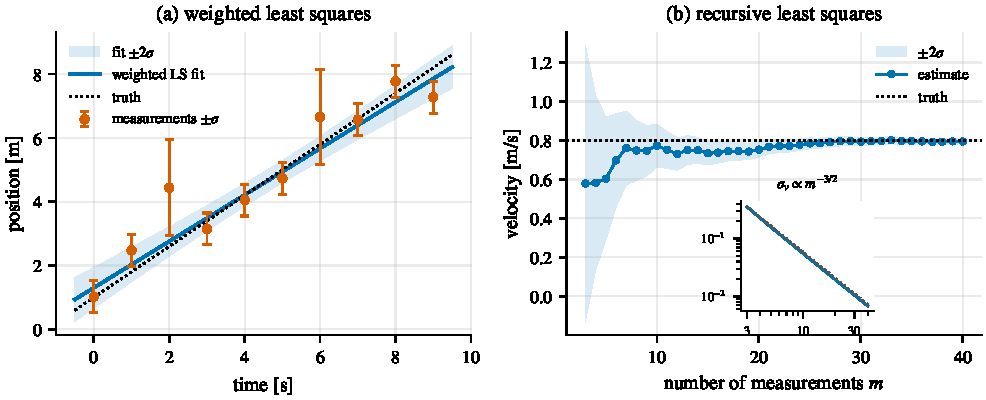
\includegraphics[width=\textwidth]{fig_lsfit.pdf}
  \caption{(a) Weighted least-squares fit of a line to noisy positions, with the $\pm2\sigma$ band of the fitted line from $(H\T R\inv H)\inv$.
  (b) Recursive least squares: the velocity estimate and its $\pm2\sigma$ bound as measurements arrive one at a time. The bound shrinks
  like $m^{-3/2}$ because later measurements also lengthen the time baseline.}
  \label{fig:lsfit}
\end{figure}

\subsection{The Gauss--Markov theorem}

Why weight by $R\inv$? Because it is the best possible linear choice.

\begin{theorem}[Gauss--Markov]
\label{thm:gauss-markov}
\index{Gauss--Markov theorem}
Among all linear unbiased estimators $\tilde x = Lz$ of $x$ in the model \eqref{eq:linear-model}, the WLS estimate \eqref{eq:wls} has the smallest
covariance: $\Cov(\tilde x) \succeq (H\T R\inv H)\inv$. It is the \term{best linear unbiased estimator} (BLUE).
\end{theorem}
\begin{proof}
Unbiasedness for every $x$ requires $LH = I$. Write $L = L_\star + D$ with $L_\star$ the WLS matrix; then $DH = 0$. The covariance is
$LRL\T = L_\star RL_\star\T + DRD\T + L_\star RD\T + DRL_\star\T$, and the cross terms vanish:
$L_\star RD\T = (H\T R\inv H)\inv H\T R\inv RD\T = (H\T R\inv H)\inv(DH)\T = 0$. So $\Cov(\tilde x) = \Cov(\hat x) + DRD\T \succeq \Cov(\hat x)$.
\end{proof}

The theorem needs no Gaussian assumption, only the first two moments of the noise. If the noise is Gaussian, more is true: WLS is the best of
\emph{all} unbiased estimators, linear or not, as the Cram\'er--Rao bound below shows.

% ==============================================================================
\section{Maximum likelihood}

\begin{definition}[Likelihood]
For a model with density $p(z\mid x)$, the \term{likelihood} of a value $x$ given observed data $z$ is $L(x) = p(z\mid x)$, viewed as a function of $x$.
The \term{maximum-likelihood} (ML) estimate maximizes it, equivalently minimizes the negative log-likelihood $-\log p(z\mid x)$.
\end{definition}

For Gaussian noise $n \sim \N(0, R)$ in $z = h(x) + n$,
\begin{equation}
  -\log p(z\mid x) = \tfrac12\big(z - h(x)\big)\T R\inv\big(z - h(x)\big) + \text{const},
\end{equation}
so ML estimation with Gaussian noise \emph{is} weighted least squares, linear or nonlinear. This is the justification of the least-squares
costs that pervade estimation, including the reprojection error of computer vision (\cref{ch:multiview}). For non-Gaussian noise, ML gives
other costs; heavy-tailed noise, for example, leads to the robust costs of \cref{ch:nlls}.

\subsection{Fisher information and the Cram\'er--Rao bound}

\begin{definition}[Fisher information]
\index{Fisher information}
For a model $p(z\mid x)$, the \term{Fisher information matrix} is
$\mathcal I(x) = \E\big[\nabla_x\log p(z\mid x)\,\nabla_x\log p(z\mid x)\T\big] = -\E\big[\nabla^2_x\log p(z\mid x)\big]$.
\end{definition}

The Fisher information measures how sharply the likelihood peaks around the true value: a likelihood that changes rapidly with $x$ pins $x$
down precisely. For the linear-Gaussian model, $\nabla^2_x\log p = -H\T R\inv H$, so $\mathcal I = H\T R\inv H$: the ``information matrix'' of WLS is the
Fisher information.

\begin{theorem}[Cram\'er--Rao lower bound]
\label{thm:crb}
\index{Cram\'er--Rao bound}
Under mild regularity conditions, every unbiased estimator satisfies $\Cov(\hat x) \succeq \mathcal I(x)\inv$.
\end{theorem}
\begin{proof}[Proof for a scalar parameter]
Let $s = \frac{\partial}{\partial x}\log p(z\mid x)$ (the \emph{score}). It has zero mean, since $\E[s] = \int\partial_xp\,\dd z = \partial_x\int p\,\dd z = 0$. Differentiating the
unbiasedness condition $\int\hat x(z)p(z\mid x)\,\dd z = x$ with respect to $x$ gives $\E[\hat x\,s] = 1$, hence $\Cov(\hat x, s) = 1$. By the
Cauchy--Schwarz inequality for covariances, $1 = \Cov(\hat x, s)^2 \le \Var(\hat x)\Var(s) = \Var(\hat x)\,\mathcal I(x)$.
\end{proof}

An unbiased estimator that attains the bound is \emph{efficient}. For the linear-Gaussian model, WLS attains it: $\Cov(\hat x) = (H\T R\inv H)\inv = \mathcal I\inv$.
No unbiased estimator can do better. This gives a precise meaning to the phrase used throughout these notes: \emph{information is inverse
covariance}, and independent measurements add their information.

% ==============================================================================
\section{Bayesian estimation}

\subsection{Priors and posteriors}

In the Bayesian view, the unknown $x$ is itself a random variable with a \emph{prior} density $p(x)$ that summarizes what is known before the
data. Bayes' rule gives the \emph{posterior} $p(x\mid z) \propto p(z\mid x)p(x)$, the complete description of what is known afterwards. Point estimates
summarize the posterior:
\begin{itemize}
  \item the \term{minimum mean-square error} (MMSE) estimate $\hat x = \E[x\mid z]$, the posterior mean;
  \item the \term{maximum a posteriori} (MAP) estimate, the posterior mode;
  \item and, ignoring the prior, the ML estimate.
\end{itemize}

\begin{theorem}[The conditional mean is optimal]
\label{thm:mmse}
Among all estimators $g(z)$, the conditional mean $\E[x\mid z]$ minimizes the Bayesian mean-square error $\E\|x - g(z)\|^2$, and indeed minimizes the
error matrix $\E[(x - g)(x - g)\T]$ in the Loewner order.
\end{theorem}
\begin{proof}
Fix $z$ and write $m = \E[x\mid z]$. For any value $g$, $\E\big[(x - g)(x - g)\T\mid z\big] = \Cov(x\mid z) + (m - g)(m - g)\T$ by the bias--variance decomposition
applied to the conditional distribution. The second term is PSD and vanishes exactly for $g = m$. Taking the expectation over $z$ preserves the
inequality.
\end{proof}

For a linear-Gaussian model the posterior is Gaussian (\cref{prop:map-ls}), so its mean and mode coincide: MMSE and MAP are the same estimate,
\begin{equation}
  \hat x = \big(P\inv + H\T R\inv H\big)\inv\big(P\inv\mu + H\T R\inv z\big), \qquad \Cov(x\mid z) = \big(P\inv + H\T R\inv H\big)\inv,
  \label{eq:bayes-linear}
\end{equation}
for a prior $\N(\mu, P)$. This is weighted least squares with one extra ``measurement'': the prior acts like a direct observation of $x$ with
value $\mu$ and covariance $P$. With an uninformative prior ($P\inv\to0$) it reduces to ML/WLS.

\subsection{Linear MMSE and the orthogonality principle}

The conditional mean can be hard to compute when distributions are not Gaussian. The best \emph{linear} (affine) estimator needs only means
and covariances.

\begin{theorem}[Linear minimum mean-square error estimator]
\label{thm:lmmse}
\index{linear MMSE estimator}\index{orthogonality principle}
Let $x$ and $z$ be random vectors with means $\mu_x$, $\mu_z$ and covariances $\Sigma_{xx}$, $\Sigma_{xz}$, $\Sigma_{zz} \succ 0$. Among estimators of the form
$\hat x = Az + b$, the mean-square error is minimized by
\begin{equation}
  \hat x = \mu_x + \Sigma_{xz}\Sigma_{zz}\inv(z - \mu_z),
  \qquad \E[(x - \hat x)(x - \hat x)\T] = \Sigma_{xx} - \Sigma_{xz}\Sigma_{zz}\inv\Sigma_{zx} .
\end{equation}
Its error is uncorrelated with the data: $\E\big[(x - \hat x)(z - \mu_z)\T\big] = 0$ (the \term{orthogonality principle}).
\end{theorem}
\begin{proof}
The error $e = x - Az - b$ has mean $\mu_x - A\mu_z - b$, which must vanish at the optimum (a non-zero mean only adds $bb\T$), so $b = \mu_x - A\mu_z$. Then
$e = (x - \mu_x) - A(z - \mu_z)$ and $\E[ee\T] = \Sigma_{xx} - A\Sigma_{zx} - \Sigma_{xz}A\T + A\Sigma_{zz}A\T$. Completing the square,
$\E[ee\T] = (A - A_\star)\Sigma_{zz}(A - A_\star)\T + \Sigma_{xx} - \Sigma_{xz}\Sigma_{zz}\inv\Sigma_{zx}$ with $A_\star = \Sigma_{xz}\Sigma_{zz}\inv$, which is minimal for $A = A_\star$. At the
optimum, $\E[e(z - \mu_z)\T] = \Sigma_{xz} - A_\star\Sigma_{zz} = 0$.
\end{proof}

The formulas are identical to Gaussian conditioning (\cref{thm:gauss-cond}): for jointly Gaussian variables the best linear estimator is the best
estimator of any kind, and for other distributions it is still the best linear one. The orthogonality principle has a geometric reading: the
estimate is the projection of $x$ onto the space of (affine) functions of the data, and the error is orthogonal to that space, exactly as a
least-squares residual is orthogonal to the column space (\cref{sec:least-squares}).

\paragraph{Application to the linear model.} For $z = Hx + n$ with prior mean $\mu$ and covariance $P$ for $x$, and noise uncorrelated with $x$:
$\mu_z = H\mu$, $\Sigma_{xz} = PH\T$, $\Sigma_{zz} = HPH\T + R$. \Cref{thm:lmmse} gives
\begin{equation}
  \hat x = \mu + K(z - H\mu), \qquad K = PH\T(HPH\T + R)\inv, \qquad \E[ee\T] = P - KHP .
  \label{eq:lmmse-update}
\end{equation}
This is the Kalman update (\cref{ch:kf}). By the Woodbury identity (\cref{thm:woodbury}) it equals \eqref{eq:bayes-linear}, but it requires
inverting an $m\times m$ matrix instead of an $n\times n$ one.

% ==============================================================================
\section{Recursive least squares}

Measurements often arrive one at a time, and recomputing \eqref{eq:wls} from scratch at each arrival would waste work. Since information adds,
the batch solution after $k$ measurements satisfies
\begin{equation}
  P_k\inv = P_{k-1}\inv + H_k\T R_k\inv H_k, \qquad P_k\inv\hat x_k = P_{k-1}\inv\hat x_{k-1} + H_k\T R_k\inv z_k,
\end{equation}
where $P_k$ is the covariance of $\hat x_k$. Rewriting this with the Woodbury identity gives the \term{recursive least squares} (RLS) update
\begin{equation}
  K_k = P_{k-1}H_k\T\big(H_kP_{k-1}H_k\T + R_k\big)\inv, \qquad
  \hat x_k = \hat x_{k-1} + K_k\big(z_k - H_k\hat x_{k-1}\big), \qquad
  P_k = (I - K_kH_k)P_{k-1} .
\end{equation}
Each step corrects the previous estimate by a gain times the \emph{innovation} $z_k - H_k\hat x_{k-1}$, the part of the new measurement that the old
estimate did not predict. It produces exactly the batch estimate at every step (\cref{fig:lsfit}b), at a cost that does not grow with the number
of measurements. RLS is the Kalman filter for a state that does not change; \cref{ch:kf} adds dynamics.

% ==============================================================================
\section{One answer, many derivations}

\begin{center}\small
\begin{tabularx}{\textwidth}{@{}l l >{\raggedright\arraybackslash}X@{}}
\toprule
Approach & Assumptions & Result for $z = Hx + n$ \\
\midrule
weighted least squares & second moments of the noise & $\hat x = (H\T R\inv H)\inv H\T R\inv z$ \\
Gauss--Markov (BLUE) & linear, unbiased & same \\
maximum likelihood & Gaussian noise & same \\
MAP / MMSE & Gaussian prior and noise & \eqref{eq:bayes-linear}: WLS with the prior as a measurement \\
linear MMSE & means and covariances only & \eqref{eq:lmmse-update}, equal to \eqref{eq:bayes-linear} \\
recursive LS & sequential data & same as batch, one measurement at a time \\
\bottomrule
\end{tabularx}
\end{center}

The Kalman filter inherits all of these interpretations. It is the exact Bayesian posterior for linear-Gaussian systems, the best linear
estimator when noises are merely uncorrelated, and a recursive least-squares solver. When models are nonlinear, these interpretations
separate, and the resulting approximations (\cref{ch:nlls,ch:nonlinear}) differ in which interpretation they try to preserve.

\begin{takeaways}
\begin{itemize}
  \item An estimator's error splits into bias and covariance: $\E[ee\T] = \Cov(\hat x) + bb\T$.
  \item Weighted least squares $\hat x = (H\T R\inv H)\inv H\T R\inv z$ has covariance $(H\T R\inv H)\inv$; information adds across independent measurements.
  \item Gauss--Markov: WLS with $R\inv$ weights is the best linear unbiased estimator.
  \item ML with Gaussian noise is least squares; the Fisher information bounds every unbiased estimator; information is inverse covariance.
  \item The conditional mean minimizes mean-square error; for Gaussians it equals the MAP estimate.
  \item The linear MMSE estimator $\mu + \Sigma_{xz}\Sigma_{zz}\inv(z - \mu_z)$ needs only second moments; its error is orthogonal to the data.
  \item Recursive least squares is the Kalman update without dynamics.
\end{itemize}
\end{takeaways}

\begin{exercises}
  \item Show that the sample mean of $m$ independent measurements of a scalar with variances $\sigma_i^2$ is not the BLUE unless all $\sigma_i$ are equal,
        and find the BLUE.
  \item For the line-fitting example with $m = 11$ measurements at $t = -5, \dots, 5$ and $\sigma = 1$, compute the covariance of $(p_0, v)$. How does it change
        if the times are $0, \dots, 10$? Interpret the off-diagonal term.
  \item Prove the matrix version of the Cram\'er--Rao bound for a linear-Gaussian model by computing $\nabla^2_x\log p$.
  \item Show that \eqref{eq:bayes-linear} and \eqref{eq:lmmse-update} agree, using \cref{thm:woodbury}.
  \item Derive the RLS update from the batch information form, and verify numerically that it reproduces the batch estimate at every step.
  \item Let $x \sim \mathcal U[-1, 1]$ and $z = x^3 + n$ with small Gaussian $n$. Compare the LMMSE estimate with the conditional mean, qualitatively. Why does
        the LMMSE estimate do poorly?
  \item A sensor reports a measurement with a bias $\beta$ that is not modeled. Show that the WLS estimate is biased by $(H\T R\inv H)\inv H\T R\inv\beta$, and explain
        why unmodeled biases are worse than large noise.
\end{exercises}
% Solutions to the exercises of Chapter 9.
\begin{solutions}
  \item The model is $z_i = x + n_i$, i.e.\ $H = \mathbf 1$ (a column of ones) and $R = \diag(\sigma_i^2)$. The WLS estimate is the BLUE
        (\cref{thm:gauss-markov}):
        \[
          \hat x = \big(\mathbf 1\T R\inv\mathbf 1\big)\inv\mathbf 1\T R\inv z = \frac{\sum_iz_i/\sigma_i^2}{\sum_i1/\sigma_i^2},
          \qquad \Var(\hat x) = \Big(\sum_i\frac{1}{\sigma_i^2}\Big)\inv,
        \]
        the inverse-variance weighted mean. The sample mean $\bar z = \frac1m\sum_iz_i$ is linear and unbiased with variance $\frac{1}{m^2}\sum_i\sigma_i^2$, and by the
        Cauchy--Schwarz inequality $\big(\sum_i\sigma_i^2\big)\big(\sum_i\sigma_i^{-2}\big) \ge m^2$, with equality only when all $\sigma_i$ are equal. So
        $\Var(\bar z) \ge \Var(\hat x)$, strictly unless the variances are equal: then (and only then) the two estimators coincide. One poor sensor can
        ruin a plain average; in the weighted one it simply counts for little.

  \item With $z_i = p_0 + vt_i + n_i$, $H$ has rows $(1, t_i)$ and $\Cov(\hat p_0, \hat v) = (H\T H)\inv$. For $t = -5, \dots, 5$, $\sum t_i = 0$ and $\sum t_i^2 = 110$, so
        \[
          (H\T H)\inv = \begin{bmatrix}11 & 0\\ 0 & 110\end{bmatrix}\inv = \diag\big(0.0909,\ 0.00909\big):
        \]
        $\sigma_{p_0} = 0.30$, $\sigma_v = 0.095$, uncorrelated. For $t = 0, \dots, 10$, $\sum t_i = 55$ and $\sum t_i^2 = 385$, and
        \[
          (H\T H)\inv = \frac{1}{1210}\begin{bmatrix}385 & -55\\ -55 & 11\end{bmatrix} = \begin{bmatrix}0.318 & -0.0455\\ -0.0455 & 0.00909\end{bmatrix}.
        \]
        The velocity variance is unchanged (it depends only on the spread of the times), but $p_0$ is now the value at the \emph{end} of the data,
        an extrapolation, with variance $3.5$ times larger and correlation $-0.85$ with $v$: a line that is too steep must start too low to pass
        through the data. The intercept is best determined at the centroid of the times, where the correlation vanishes.

  \item For $z = Hx + n$ with $n \sim \N(0, R)$, $\log p(z\mid x) = -\tfrac12(z - Hx)\T R\inv(z - Hx) + \text{const}$. Its gradient is
        $\nabla_x\log p = H\T R\inv(z - Hx)$ and its Hessian $\nabla_x^2\log p = -H\T R\inv H$, which does not depend on $z$, so
        $\mathcal I(x) = -\E[\nabla_x^2\log p] = H\T R\inv H$. (The outer-product definition agrees: $\E[H\T R\inv nn\T R\inv H] = H\T R\inv H$.) The matrix bound is
        proved like the scalar one: for an unbiased $\hat x$ and the score $s = \nabla_x\log p$, differentiating $\E[\hat x] = x$ gives $\Cov(\hat x, s) = I$, and
        the covariance matrix of $(\hat x, s)$,
        $\begin{bmatrix}\Cov(\hat x) & I\\ I & \mathcal I\end{bmatrix} \succeq 0$, has the PSD Schur complement $\Cov(\hat x) - \mathcal I\inv \succeq 0$ (Exercise 3.3's argument).
        WLS has covariance $(H\T R\inv H)\inv = \mathcal I\inv$ and attains the bound.

  \item Apply \cref{thm:woodbury} (as in Exercise 3.6) to the covariance of \eqref{eq:bayes-linear}:
        $(P\inv + H\T R\inv H)\inv = P - PH\T(HPH\T + R)\inv HP = P - KHP$ with $K = PH\T(HPH\T + R)\inv$, the covariance of \eqref{eq:lmmse-update}. For the mean,
        multiply out with this expression:
        \[
          (P - KHP)\big(P\inv\mu + H\T R\inv z\big) = \mu - KH\mu + \big(PH\T - KHPH\T\big)R\inv z .
        \]
        Since $K(HPH\T + R) = PH\T$, we have $PH\T - KHPH\T = KR$, so the last term is $Kz$, and the mean is $\mu + K(z - H\mu)$: the two forms agree.

  \item With prior $(\hat x_0, P_0)$, the batch estimate after $k$ measurements has information $P_k\inv = P_0\inv + \sum_{i\le k}H_i\T R_i\inv H_i$ and information
        vector $P_k\inv\hat x_k = P_0\inv\hat x_0 + \sum_{i\le k}H_i\T R_i\inv z_i$. Subtracting the expressions for $k - 1$ gives the recursion in information form
        stated in the chapter. Solving it for $\hat x_k$: $\hat x_k = P_k\big(P_{k-1}\inv\hat x_{k-1} + H_k\T R_k\inv z_k\big)$, and with
        $P_{k-1}\inv = P_k\inv - H_k\T R_k\inv H_k$ this is $\hat x_k = \hat x_{k-1} + P_kH_k\T R_k\inv(z_k - H_k\hat x_{k-1})$. Finally $P_kH_k\T R_k\inv = K_k$ (the
        push-through identity of Exercise 5.6) and $P_k = (I - K_kH_k)P_{k-1}$ by Woodbury. A numerical check with three unknowns, thirty scalar
        measurements of random variances and a weak prior: the RLS estimate and covariance agree with the batch solution after every
        measurement to $3\times10^{-12}$.

  \item The LMMSE estimate uses only second moments: with $\E[x] = \E[z] = 0$, $\Sigma_{xz} = \E[x^4] = \tfrac15$ and $\Sigma_{zz} = \E[x^6] + \sigma^2 = \tfrac17 + \sigma^2$,
        \[
          \hat x_{\mathrm{LMMSE}} = \frac{1/5}{1/7 + \sigma^2}\,z \approx 1.4\,z ,
        \]
        a straight line through a cube-root-shaped relation. The conditional mean $\E[x\mid z]$ follows the cube root, $\approx z^{1/3}$ wherever the noise is
        small compared with $z$. At $x = 0.5$ ($z = 0.125$) the LMMSE estimate is $0.17$, at $x = 0.9$ ($z = 0.73$) it is $1.02$, outside the support of $x$;
        the conditional mean gives $0.50$ and $0.90$. Overall, for $\sigma = 0.01$, the LMMSE root-mean-square error is $0.23$ against $0.075$ for the
        conditional mean (computed numerically). LMMSE does poorly because the dependence of $z$ on $x$ is strongly nonlinear: the best straight line
        fits neither small nor large values. This is the limitation the EKF inherits, mitigated by linearizing locally around the current estimate
        rather than globally.

  \item With $z = Hx + n + \beta$, the estimate $\hat x = Lz$ with $L = (H\T R\inv H)\inv H\T R\inv$ satisfies $LH = I$, so
        \[
          \hat x - x = Ln + L\beta, \qquad \E[\hat x] - x = (H\T R\inv H)\inv H\T R\inv\beta .
        \]
        The noise term has zero mean and covariance $(H\T R\inv H)\inv$, which shrinks as measurements accumulate ($\propto 1/m$ for $m$ comparable measurements).
        The bias term does not shrink: a constant offset in every measurement is averaged, not cancelled. The estimate therefore converges,
        with ever-smaller reported covariance, to the wrong value, and the filter becomes overconfident. Large noise is honest: it is in $R$, so it
        makes the covariance large. An unmodeled bias is invisible to the covariance and, if $\beta$ lies in the range of $H$, invisible in the residuals
        too, because it is indistinguishable from a different $x$. The cure is to model the bias as a state (\cref{ch:processes}), which is exactly
        why IMU biases are part of the filter state.
\end{solutions}


\chapter[Nonlinear Least Squares and Optimization]{Nonlinear Least Squares\\ and Optimization}
\label{ch:nlls}
\chaptermark{Nonlinear Least Squares} % short running header

\begin{objectives}
\begin{itemize}
  \item Formulate estimation problems with nonlinear models as nonlinear least-squares problems.
  \item Derive Newton, Gauss--Newton and Levenberg--Marquardt iterations, and understand when each converges.
  \item Optimize over manifolds such as $\SO$ by iterating in the tangent space.
  \item Make least squares robust to outliers with M-estimators and iteratively reweighted least squares.
  \item Exploit the structure of problems with poses and landmarks: the Schur complement and marginalization.
  \item See that an extended Kalman update is one Gauss--Newton step, the bridge between filtering and optimization.
\end{itemize}
\end{objectives}

Most measurement models in VIO are nonlinear: projections divide by depth, rotations enter through trigonometric functions. Maximum
likelihood with Gaussian noise then becomes a \emph{nonlinear} least-squares problem with no closed-form solution. This chapter develops the
iterative methods that solve such problems. They are used directly in this project for triangulation, and they explain what the extended
Kalman filter and the MSCKF are doing.

% ==============================================================================
\section{The problem}

Given residual functions $r_i(x)$ (measurement minus prediction) with noise covariances $R_i$, the maximum-likelihood estimate minimizes
\begin{equation}
  F(x) = \frac12\sum_i r_i(x)\T R_i\inv r_i(x) = \frac12\,r(x)\T W\,r(x),
  \label{eq:nlls}
\end{equation}
where $r$ stacks the residuals and $W = \blkdiag(R_i\inv)$. Examples in these notes:
\begin{itemize}
  \item \emph{Triangulation}: find a 3D point minimizing the reprojection errors in several images (\cref{ch:multiview}).
  \item \emph{Relative pose}: find the motion between two images that best explains point correspondences.
  \item \emph{Bundle adjustment}: find all camera poses and all points at once.
  \item \emph{Sliding-window VIO}: find a window of states minimizing visual and inertial residuals together.
\end{itemize}
Writing $W = L\T L$ (for instance $L$ the inverse of a Cholesky factor of the noise covariance) and replacing $r$ by $Lr$ \emph{whitens} the residuals,
so that $W = I$. We do this silently when convenient.

% ==============================================================================
\section{Descent methods}

The gradient and Hessian of $F$ follow from the chain rule. With $J = \partial r/\partial x$,
\begin{equation}
  \nabla F = J\T Wr, \qquad \nabla^2F = J\T WJ + \sum_k(Wr)_k\,\nabla^2r_k .
  \label{eq:nlls-derivatives}
\end{equation}

\paragraph{Gradient descent.} Step downhill, $x \gets x - \alpha\nabla F$, with a step length $\alpha$ chosen by a line search. It always makes progress for small
enough $\alpha$, but it ignores curvature and zig-zags slowly along narrow valleys.

\paragraph{Newton's method.} Minimize the quadratic Taylor model $F(x + \delta) \approx F + \nabla F\T\delta + \tfrac12\delta\T\nabla^2F\,\delta$ exactly:
\begin{equation}
  \nabla^2F\,\delta = -\nabla F .
\end{equation}
Near a minimum with positive-definite Hessian, Newton's method converges \emph{quadratically}: the number of correct digits roughly doubles each
iteration. But it needs second derivatives of every residual, and far from the minimum the Hessian may not be positive definite, in which case the
step can go uphill.

% ==============================================================================
\section{Gauss--Newton}
\label{sec:gauss-newton}

\index{Gauss--Newton method}
Least-squares problems allow a better compromise. Linearize the \emph{residuals} rather than the cost: $r(x + \delta) \approx r + J\delta$. The cost then
becomes a linear least-squares problem in $\delta$,
\begin{equation}
  \min_\delta\ \tfrac12\|r + J\delta\|_W^2
  \quad\Longrightarrow\quad
  \big(J\T WJ\big)\,\delta = -J\T Wr,
  \label{eq:gn-step}
\end{equation}
the \term{Gauss--Newton} step. Comparing with \eqref{eq:nlls-derivatives}, Gauss--Newton is Newton's method with the second term of the Hessian dropped.
That term is small when the residuals are small at the solution, or when the residuals are nearly linear, which is the common case for
well-modeled sensors. Then Gauss--Newton converges almost as fast as Newton, without second derivatives. The approximate Hessian $J\T WJ$ is
always positive semi-definite, so the step is always a descent direction (if $J$ has full column rank).

\begin{algorithm}[h]
\caption{Gauss--Newton}
\label{alg:gauss-newton}
\begin{algorithmic}[1]
\Require initial guess $x$, residual function $r(x)$ and its Jacobian $J(x)$
\Repeat
  \State evaluate $r$ and $J$ at $x$
  \State solve $(J\T WJ)\,\delta = -J\T Wr$ \Comment{Cholesky of $J\T WJ$, or QR of the whitened $J$}
  \State $x \gets x + \delta$
\Until{$\|\delta\|$ or the decrease of $F$ is below a tolerance}
\end{algorithmic}
\end{algorithm}

The linear system is the normal equation of a linear least-squares problem, so all the numerical advice of \cref{sec:least-squares} applies: for
small, well-conditioned problems Cholesky of $J\T WJ$ is fine; for ill-conditioned ones, QR of the whitened Jacobian is safer.

\paragraph{When Gauss--Newton fails.} With a poor initial guess, large residuals or strong nonlinearity, the linear model can be a bad
approximation, and a full step can increase the cost. If $J\T WJ$ is singular, some direction is not determined by the data (a \emph{gauge freedom}
or an unobservable direction), and the step is undefined.

\section{Levenberg--Marquardt}

\index{Levenberg--Marquardt method}
The \term{Levenberg--Marquardt} (LM) method damps the Gauss--Newton step:
\begin{equation}
  \big(J\T WJ + \lambda D\big)\,\delta = -J\T Wr, \qquad \lambda \ge 0,
\end{equation}
with $D = I$ or $D = \diag(J\T WJ)$. For $\lambda\to0$ it is Gauss--Newton; for large $\lambda$ the step becomes a short gradient-descent step. The damping is
adapted to how well the linear model predicted the actual change of cost. With the \emph{gain ratio}
\begin{equation}
  \rho = \frac{F(x) - F(x + \delta)}{F(x) - \tfrac12\|r + J\delta\|_W^2},
\end{equation}
a step with $\rho$ close to one is accepted and $\lambda$ decreased (trust the model more), while a step with small or negative $\rho$ is rejected and
$\lambda$ increased. LM is equivalent to a \emph{trust-region} method that restricts the step to a region where the linearization is trusted. It is
the default solver of most computer-vision and robotics libraries.

\begin{figure}[t]
  \centering
  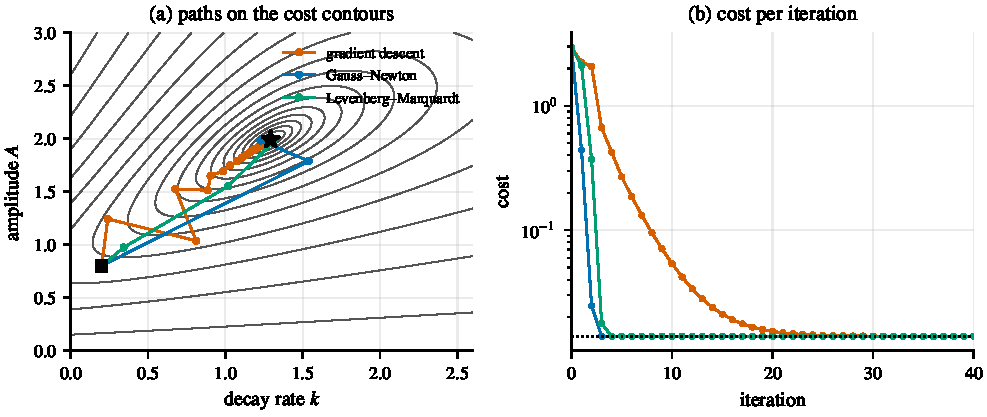
\includegraphics[width=\textwidth]{fig_gn_lm.pdf}
  \caption{Fitting the decay rate and amplitude of an exponential to noisy data. (a) Paths of gradient descent, Gauss--Newton and
  Levenberg--Marquardt on the contours of the cost, from the same starting point. (b) Cost versus iteration. Gradient descent crawls along the
  curved valley; Gauss--Newton and LM reach the minimum in a handful of iterations.}
  \label{fig:gn-lm}
\end{figure}

\section{Uncertainty of the solution}

At the minimum $\hat x$, the cost is approximately quadratic, $F(\hat x + \delta) \approx F(\hat x) + \tfrac12\delta\T(J\T WJ)\delta$, and with $W$ equal to the inverse
noise covariance the estimate has approximately the WLS covariance of the linearized problem (\cref{prop:wls-cov}):
\begin{equation}
  \Cov(\hat x) \approx \big(J\T WJ\big)\inv\Big|_{\hat x} .
\end{equation}
This is the \emph{Laplace approximation}: the posterior is replaced by a Gaussian fitted to its peak. It is accurate when the problem is nearly
linear over the region of uncertainty. A triangulated point, for example, gets a covariance from the Jacobians of its reprojection errors.

% ==============================================================================
\section{Optimization on manifolds}
\label{sec:manifold-opt}

When the unknown includes rotations, $x + \delta$ is replaced by the retraction $x\bplus\delta$ of \cref{ch:lie}. Linearize the residual in the tangent space,
$r(x\bplus\delta) \approx r(x) + J\delta$ with $J$ the manifold Jacobian (\cref{def:manifold-jacobian}), solve the same Gauss--Newton equation for $\delta$, and
update $x \gets x\bplus\delta$. The step is computed in a flat space and applied on the curved one, so the iterate never leaves the manifold and no
constraint ever needs enforcing. Covariances are then expressed in the tangent space at the solution, exactly as in a filter.

\begin{example}[Rotation averaging as Gauss--Newton]
Average rotations $R_1, \dots, R_N$ (\cref{ch:lie}) by minimizing $\tfrac12\sum_i\|r_i\|^2$ with $r_i(\bar R) = \Log(\bar R\T R_i)$. Perturbing
$\bar R\bplus\delta = \bar R\Exp(\delta)$ gives $r_i = \Log(\Exp(-\delta)\bar R\T R_i) \approx r_i(\bar R) - \Jlinv(r_i)\,\delta$ (\cref{eq:bch-left}). For small residuals
$\Jlinv \approx I$, so $J_i \approx -I$, and the Gauss--Newton step is $\delta = \frac1N\sum_ir_i$: exactly the averaging iteration of \cref{ch:lie}.
\end{example}

% ==============================================================================
\section{Robust estimation}
\label{sec:robust}

\subsection{Outliers break least squares}

A squared cost gives enormous influence to large residuals: a single wrong measurement, far from the others, can drag a least-squares estimate
arbitrarily far. Real data contain such \term{outliers}: misassociated features, reflections, moving objects. Two defenses exist: detect and
remove them (gating, RANSAC), or reduce their influence with a robust cost.

\subsection{M-estimators}

\index{M-estimator}\index{robust kernel}
An \term{M-estimator} replaces the quadratic by a function $\rho$ of the whitened residual norm $s_i = \|r_i\|_{R_i\inv}$:
\begin{equation}
  \min_x\ \sum_i\rho(s_i) .
\end{equation}

\begin{center}\small
\begin{tabular}{@{}l l l@{}}
\toprule
Kernel & $\rho(s)$ & weight $w(s) = \rho'(s)/s$ \\
\midrule
least squares & $\tfrac12s^2$ & $1$ \\
Huber & $\tfrac12s^2$ for $s\le c$;\ \ $c(s - \tfrac c2)$ otherwise & $1$ for $s \le c$;\ \ $c/s$ otherwise \\
Cauchy & $\tfrac{c^2}2\log(1 + s^2/c^2)$ & $1/(1 + s^2/c^2)$ \\
Tukey & $\tfrac{c^2}6\big(1 - (1 - s^2/c^2)^3\big)$ for $s \le c$;\ \ $c^2/6$ otherwise & $(1 - s^2/c^2)^2$ for $s \le c$;\ \ $0$ otherwise \\
\bottomrule
\end{tabular}
\end{center}

\begin{figure}[t]
  \centering
  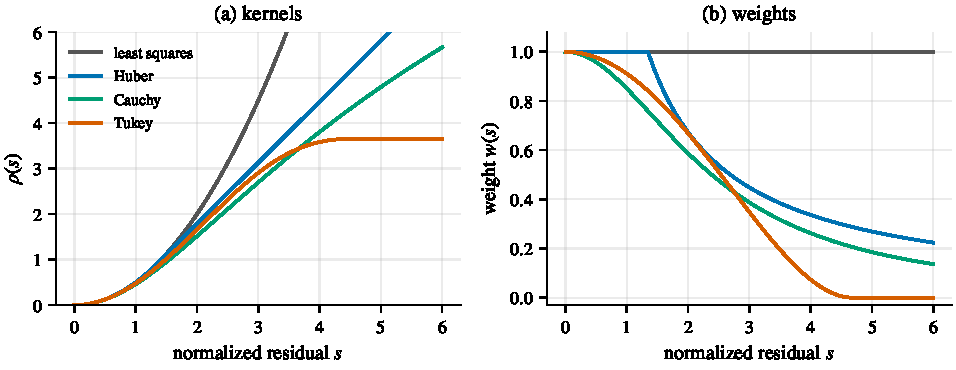
\includegraphics[width=\textwidth]{fig_robust_kernels.pdf}
  \caption{Robust kernels (left) and their weights (right) as functions of the normalized residual, for $c = 1.345$ (Huber), $2.385$ (Cauchy) and
  $4.685$ (Tukey). Huber grows linearly instead of quadratically for large residuals; Cauchy grows logarithmically; Tukey ignores residuals beyond
  $c$ entirely.}
  \label{fig:robust-kernels}
\end{figure}

The derivative $\psi = \rho'$ (the \emph{influence function}) measures how hard a residual pulls on the estimate: unbounded and linear for least squares,
bounded for Huber, decreasing to zero for Cauchy and Tukey (\cref{fig:robust-kernels}). The constants $c$ trade efficiency on clean Gaussian data against
robustness; the values in the figure keep 95\% of the efficiency of least squares on Gaussian noise.

\subsection{Iteratively reweighted least squares}

Setting the gradient of $\sum_i\rho(s_i)$ to zero gives $\sum_iw(s_i)J_i\T R_i\inv r_i = 0$ with $w(s) = \rho'(s)/s$: the normal equations of a \emph{weighted}
least-squares problem whose weights depend on the residuals. \emph{Iteratively reweighted least squares} (IRLS) alternates: compute the weights
from the current residuals, take a Gauss--Newton step with those weights, repeat. Outliers receive small weights and stop dominating. Robust
kernels need a reasonable initial guess, because with large initial errors every residual looks like an outlier; RANSAC (\cref{ch:multiview})
provides such guesses.

Gating, used in filters, is the hard-decision version of the same idea: a measurement whose normalized residual exceeds a threshold gets weight
zero, all others weight one, a ``truncated quadratic'' kernel.

% ==============================================================================
\section{Structure: poses, landmarks and the Schur complement}
\label{sec:schur-ba}

Many estimation problems have two kinds of unknowns. In bundle adjustment, the cameras $c$ and the landmarks $l$; in VIO smoothing, the states in
a window and the features. Each residual involves one camera and one landmark, so the normal equations have a special block structure:
\begin{equation}
  \begin{bmatrix} A & B \\ B\T & C \end{bmatrix}\begin{bmatrix}\delta c\\ \delta l\end{bmatrix} = \begin{bmatrix}g_c\\ g_l\end{bmatrix},
\end{equation}
where $C$, the landmark block of $J\T WJ$, is block diagonal with one $3\times3$ block per landmark (no residual involves two landmarks). Inverting $C$ is
therefore cheap. Eliminating the landmarks with the Schur complement (\cref{sec:schur}),
\begin{equation}
  \big(A - BC\inv B\T\big)\,\delta c = g_c - BC\inv g_l, \qquad \delta l = C\inv(g_l - B\T\delta c),
  \label{eq:reduced-camera-system}
\end{equation}
leaves a \emph{reduced camera system} whose size depends only on the number of cameras, often a hundred times smaller than the full problem.

\begin{figure}[t]
  \centering
  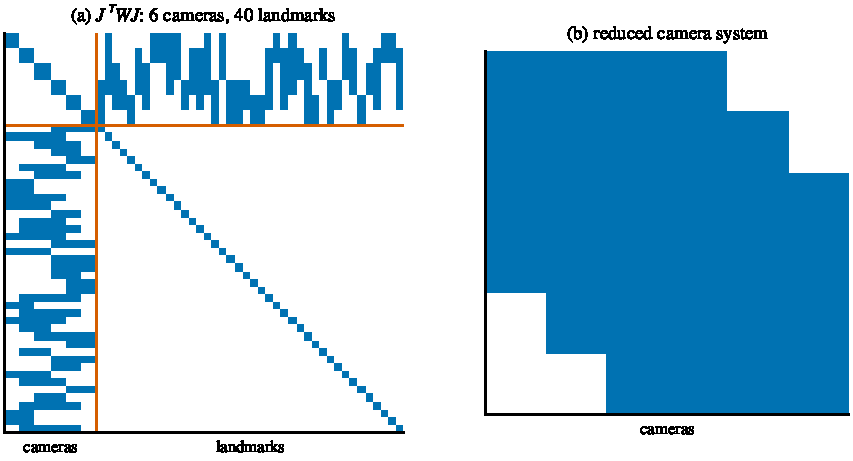
\includegraphics[width=\textwidth]{fig_ba_sparsity.pdf}
  \caption{Sparsity of the normal-equation matrix $J\T WJ$ for a toy bundle adjustment with 6 cameras and 40 landmarks (left), and of the reduced camera
  system after eliminating the landmarks (right). The landmark block is block-diagonal and cheap to eliminate; the reduced system is small but dense.}
  \label{fig:ba-sparsity}
\end{figure}

The same operation has a probabilistic meaning. $J\T WJ$ is the information matrix of the linearized problem, and the Schur complement is
\emph{marginalization in information form} (\cref{thm:gauss-cond}): the reduced system is the information that the measurements carry about the
cameras alone, after the landmarks have been integrated out. Sliding-window estimators use exactly this to discard old states, keeping their
information as a Gaussian prior on the remaining ones; the price is \emph{fill-in}, since the reduced matrix is dense (\cref{fig:ba-sparsity}). The
MSCKF performs the same elimination of each landmark, by a different algebraic route: the left-nullspace projection (\cref{ch:msckfupdate}).

% ==============================================================================
\section{Filtering as optimization}
\label{sec:filter-gn}

\begin{proposition}[The EKF update is one Gauss--Newton step]
\label{prop:ekf-gn}
\index{iterated EKF}
Consider the MAP cost of one measurement $z = h(x) + n$, $n \sim \N(0, R)$, with prior $\N(\mu, P)$:
\begin{equation*}
  F(x) = \tfrac12\|x - \mu\|^2_{P\inv} + \tfrac12\|z - h(x)\|^2_{R\inv}.
\end{equation*}
One Gauss--Newton step from $x = \mu$ gives $x^+ = \mu + K(z - h(\mu))$ with $K = PH\T(HPH\T + R)\inv$ and $H = \partial h/\partial x|_\mu$: the extended
Kalman update (\cref{ch:nonlinear}).
\end{proposition}
\begin{proof}
The stacked residual is $r(x) = \big(L_P(x - \mu),\ L_R(h(x) - z)\big)$ with $L_P\T L_P = P\inv$ and $L_R\T L_R = R\inv$. At $x = \mu$, $r = (0,\ L_R(h(\mu) - z))$ and
$J = (L_P,\ L_RH)$, so the Gauss--Newton equation \eqref{eq:gn-step} reads $(P\inv + H\T R\inv H)\delta = H\T R\inv(z - h(\mu))$. By the Woodbury identity,
$(P\inv + H\T R\inv H)\inv H\T R\inv = PH\T(HPH\T + R)\inv = K$.
\end{proof}

Iterating the Gauss--Newton step, re-linearizing $h$ at each new estimate while keeping the prior term, gives the \emph{iterated} EKF, which
handles strong measurement nonlinearities better. Sliding-window smoothers go further and re-linearize past measurements as well. The MSCKF update
is one Gauss--Newton step of a sliding-window problem whose landmarks have been eliminated (\cref{ch:msckfupdate}): filtering and optimization
are two ends of one spectrum, distinguished by how often they re-linearize and which variables they keep.

\begin{takeaways}
\begin{itemize}
  \item ML with Gaussian noise means minimizing $\tfrac12 r\T Wr$; the gradient is $J\T Wr$ and $J\T WJ$ approximates the Hessian.
  \item Gauss--Newton solves $(J\T WJ)\delta = -J\T Wr$ repeatedly; it converges fast when residuals are small or nearly linear.
  \item Levenberg--Marquardt damps the step adaptively and is robust to poor initial guesses.
  \item On manifolds, compute the step in the tangent space and apply it with $\bplus$.
  \item $(J\T WJ)\inv$ at the optimum approximates the covariance of the estimate.
  \item Robust kernels bound the influence of outliers; IRLS solves them; gating is the hard version.
  \item Eliminating landmarks with the Schur complement is marginalization in information form.
  \item An EKF update is one Gauss--Newton step on the MAP cost; iterating gives the iterated EKF.
\end{itemize}
\end{takeaways}

\begin{exercises}
  \item Derive the gradient and Hessian \eqref{eq:nlls-derivatives} of the least-squares cost.
  \item Implement Gauss--Newton and LM for fitting $y = ae^{-bt}$ to noisy data and reproduce \cref{fig:gn-lm}. Start from a poor initial guess and compare
        robustness.
  \item Show that for a zero-residual problem Gauss--Newton converges quadratically near the solution.
  \item Fit a line to data containing 20\% gross outliers with least squares, Huber IRLS and Cauchy IRLS. Compare the results.
  \item Implement the Schur-complement solution \eqref{eq:reduced-camera-system} for a random sparse problem and verify that it matches the full solve.
  \item Prove that the reduced camera system equals the inverse of the camera block of $(J\T WJ)\inv$, and interpret this as marginalization.
  \item Write out one iteration of the iterated EKF and show that it reduces to the standard EKF update after the first iteration.
\end{exercises}

\chapter{Linear Dynamical Systems}
\label{ch:linsys}

\begin{objectives}
\begin{itemize}
  \item Write physical systems in continuous- and discrete-time state-space form.
  \item Discretize deterministic inputs and white process noise exactly and approximately, including Van Loan's method.
  \item Understand stability, and why inertial errors grow polynomially.
  \item Define observability, test it with the observability matrix, and compute unobservable directions.
  \item Understand what observability means for the covariance of a Kalman filter.
\end{itemize}
\end{objectives}

The Kalman filter is built on a linear state-space model. This chapter collects the linear systems theory it needs: how to write a model, how
to turn a continuous-time model into the discrete-time form a computer processes, and how to decide whether the measurements can determine the
state at all.

% ==============================================================================
\section{State-space models}

A continuous-time linear \term{state-space model} has the form
\begin{equation}
  \dot x(t) = F(t)\,x(t) + B(t)\,u(t) + G(t)\,w(t), \qquad z(t) = H(t)\,x(t) + n(t),
  \label{eq:ct-model}
\end{equation}
with state $x$, known input $u$, white process noise $w$ (density $Q_c$), measurement $z$ and measurement noise $n$. The state is the smallest set of
numbers whose present value, together with future inputs and noises, determines the future. Its discrete-time counterpart is
\begin{equation}
  x_{k+1} = \Phi_k\,x_k + \Gamma_k\,u_k + w_k, \qquad z_k = H_k\,x_k + n_k,
  \qquad w_k \sim \N(0, Q_k),\ n_k \sim \N(0, R_k).
  \label{eq:dt-model}
\end{equation}

\begin{example}[Models used in these notes]
\label{ex:state-models}
\begin{itemize}
  \item \emph{Constant velocity}: $x = (p, v)$, $\dot p = v$, $\dot v = w$ (white acceleration). $F = \begin{bmatrix}0 & 1\\0 & 0\end{bmatrix}$, $G = \begin{bmatrix}0\\1\end{bmatrix}$.
  \item \emph{Random-walk bias}: $\dot b = w_b$. $F = 0$, $G = 1$.
  \item \emph{Inertial error model} (one axis, preview of \cref{ch:errordyn}): $\delta\dot p = \delta v$, $\delta\dot v = g\,\delta\theta - \delta b_a - n_a$,
        $\delta\dot\theta = -\delta b_g - n_g$, plus random-walk biases. A chain of integrators driven by noise.
\end{itemize}
\end{example}

The discrete-time solution follows by repeated substitution:
\begin{equation}
  x_k = \Phi(k, 0)\,x_0 + \sum_{j=0}^{k-1}\Phi(k, j+1)\big(\Gamma_ju_j + w_j\big), \qquad \Phi(k, j) = \Phi_{k-1}\Phi_{k-2}\cdots\Phi_j,
\end{equation}
the discrete analog of the variation-of-constants formula (\cref{prop:stm}).

% ==============================================================================
\section{Discretization}
\label{sec:discretization}

Physical laws are continuous, computers are discrete. Over a step $\Dt$ in which $F$, $B$ and $G$ are constant, the solution of \eqref{eq:ct-model}
(\cref{thm:lti-solution}) is
\begin{equation}
  x(t + \Dt) = \underbrace{e^{F\Dt}}_{\Phi}\,x(t) + \int_0^\Dt e^{Fs}B\,u(t + \Dt - s)\,\dd s + \underbrace{\int_0^\Dt e^{Fs}G\,w(t + \Dt - s)\,\dd s}_{w_k},
\end{equation}
which has exactly the discrete form \eqref{eq:dt-model}.

\paragraph{Deterministic inputs.} If the input is held constant over the step (a \emph{zero-order hold}, which is what a sampled IMU reading
means), the input term is $\Gamma u_k$ with $\Gamma = \int_0^\Dt e^{Fs}\,\dd s\,B$. Both $\Phi$ and $\Gamma$ come from one matrix exponential,
\begin{equation}
  \exp\!\Big(\begin{bmatrix} F & B \\ 0 & 0\end{bmatrix}\Dt\Big) = \begin{bmatrix} \Phi & \Gamma \\ 0 & I\end{bmatrix},
\end{equation}
which can be verified by noting that both sides solve the same matrix ODE in $\Dt$.

\paragraph{Process noise.} The discrete noise $w_k$ is a weighted integral of white noise, so it is zero-mean Gaussian with covariance (by the
same calculation as in \cref{prop:lyapunov})
\begin{equation}
  Q_d = \int_0^\Dt e^{Fs}\,GQ_cG\T\,e^{F\T s}\,\dd s .
  \label{eq:qd-exact}
\end{equation}

\subsection{Approximations}

Expanding to first order in $\Dt$ gives the approximations used by most real-time filters and frozen in AGENTS.md F2:
\begin{equation}
  \Phi \approx I + F\Dt, \qquad Q_d \approx GQ_cG\T\,\Dt .
  \label{eq:disc-first-order}
\end{equation}
Both are accurate to $O(\Dt^2)$ per step. The units confirm the second: a noise density $\sigma_a$ in $\mathrm{m/s^2/\sqrt{Hz}}$ gives $\sigma_a^2\Dt$ in
$\mathrm{m^2/s^2}$, a velocity variance. A second-order option adds $\tfrac12F^2\Dt^2$ to $\Phi$ and $\tfrac12(FGQ_cG\T + GQ_cG\T F\T)\Dt^2$ to $Q_d$.

\begin{example}[Double integrator]
\label{ex:double-integrator-qd}
For position and velocity driven by white acceleration of density $\sigma$, $F = \begin{bmatrix}0&1\\0&0\end{bmatrix}$, $G = \begin{bmatrix}0\\1\end{bmatrix}$, $Q_c = \sigma^2$.
\Cref{ex:double-integrator} gives $e^{Fs}G = [s;\ 1]$, so \eqref{eq:qd-exact} evaluates exactly to
\begin{equation}
  Q_d = \sigma^2\begin{bmatrix} \Dt^3/3 & \Dt^2/2 \\ \Dt^2/2 & \Dt \end{bmatrix}.
\end{equation}
The first-order approximation $Q_d \approx \diag(0, \sigma^2\Dt)$ puts no noise on position within a single step. Yet after $n$ steps of exact $\Phi$, the
accumulated position variance is $\sum_{k=1}^{n} (k\Dt)^2\sigma^2\Dt \to \sigma^2 t^3/3$ as $\Dt\to0$ (a Riemann sum), which is the exact answer of
\cref{prop:integrated-noise}. The per-step error of the approximation does not accumulate into a wrong growth law; it only introduces an $O(\Dt)$
relative error, negligible at 200~Hz.
\end{example}

\subsection{Van Loan's method}

When higher accuracy is wanted, \eqref{eq:qd-exact} can be computed exactly with a single matrix exponential~\cite{vanloan1978}.

\begin{proposition}[Van Loan]
\label{prop:vanloan}
\index{Van Loan's method}
Let $C = \exp\!\Big(\begin{bmatrix} -F & GQ_cG\T \\ 0 & F\T \end{bmatrix}\Dt\Big) = \begin{bmatrix} C_{11} & C_{12} \\ 0 & C_{22}\end{bmatrix}$. Then
$\Phi = C_{22}\T$ and $Q_d = \Phi\, C_{12}$.
\end{proposition}
\begin{proof}
For a block upper-triangular generator, the diagonal blocks of the exponential are the exponentials of the diagonal blocks, so $C_{22} = e^{F\T\Dt}$.
The off-diagonal block, as a function of $\Dt$, satisfies $\dot C_{12} = -FC_{12} + GQ_cG\T C_{22}$ with $C_{12}(0) = 0$, whose solution (variation of constants)
is $C_{12} = \int_0^\Dt e^{-F(\Dt - s)}\,GQ_cG\T\,e^{F\T s}\,\dd s$. Multiplying by $\Phi = e^{F\Dt}$ on the left, and using
$e^{F\Dt}e^{-F(\Dt - s)} = e^{Fs}$, gives $\Phi C_{12} = \int_0^\Dt e^{Fs}\,GQ_cG\T\,e^{F\T s}\,\dd s$, which is \eqref{eq:qd-exact}.
\end{proof}

For the 15-state inertial error model this costs a $30\times30$ matrix exponential per step, too expensive at 200~Hz but an excellent test oracle for the
closed forms of \cref{ch:errordyn}.

% ==============================================================================
\section{Stability}

A linear time-invariant system is \emph{stable} if its free response decays. For $\dot x = Fx$ the modes are $e^{\lambda_it}$ (\cref{thm:lti-solution}), so the
system is asymptotically stable when all eigenvalues of $F$ have negative real parts. For $x_{k+1} = \Phi x_k$ the modes are $\lambda_i^k$, so all eigenvalues of
$\Phi$ must lie strictly inside the unit circle; the two conditions correspond through $\lambda_\Phi = e^{\lambda_F\Dt}$.

Integrators have eigenvalues at zero (continuous) or one (discrete): they are \emph{marginally} stable. A single integrator holds its state; a chain of
integrators (a nilpotent $F$) makes initial errors grow \emph{polynomially}, like $t$, $t^2$, $t^3$. The error dynamics of inertial navigation are of this
kind (\cref{ex:state-models}), which is why IMU errors grow polynomially rather than exponentially, and why they never stop growing without aiding.

% ==============================================================================
\section{Observability}
\label{sec:observability-linear}

\subsection{Definition and the observability matrix}

\begin{definition}[Observability]
\index{observability}
A system is \term{observable} if the initial state $x_0$ can be determined from the inputs and the noise-free outputs over a finite time.
\end{definition}

Because the inputs are known, their contribution to the outputs can be subtracted, so observability depends only on $(\Phi, H)$. For a discrete
time-invariant system without noise, $z_k = H\Phi^kx_0$. Stacking the first $n$ outputs,
\begin{equation}
  \begin{bmatrix} z_0 \\ z_1 \\ \vdots \\ z_{n-1}\end{bmatrix} = \underbrace{\begin{bmatrix} H \\ H\Phi \\ \vdots \\ H\Phi^{n-1}\end{bmatrix}}_{\mathcal O}x_0 .
\end{equation}

\begin{theorem}[Observability rank test]
\label{thm:obs-rank}
\index{observability matrix}
The system is observable if and only if the \term{observability matrix} $\mathcal O$ has rank $n$. Its nullspace is the \term{unobservable subspace}: the
initial states that produce identically zero output forever.
\end{theorem}
\begin{proof}
If $\mathcal O$ has full column rank, $x_0$ is the unique solution of the stacked equations. If $\mathcal Ox_0 = 0$ for some $x_0 \ne 0$, then $H\Phi^kx_0 = 0$ for
$k < n$, and by the Cayley--Hamilton theorem ($\Phi^n$ is a linear combination of $I, \Phi, \dots, \Phi^{n-1}$) also for all $k \ge n$; such an $x_0$ is
indistinguishable from zero. More outputs never add rank beyond the first $n$.
\end{proof}

The unobservable subspace is invariant under $\Phi$: an unobservable error stays unobservable as the system evolves. For time-varying systems, the
same reasoning gives $\mathcal O = [H_0;\ H_1\Phi(1, 0);\ H_2\Phi(2, 0);\ \dots]$, and observability can depend on the trajectory, a fact that matters
greatly for VIO (\cref{ch:observability}).

\subsection{Examples}

\begin{example}[Position versus velocity measurements]
For the discretized constant-velocity model, $\Phi = \begin{bmatrix}1 & \Dt\\0 & 1\end{bmatrix}$.
\begin{itemize}
  \item Measuring position, $H = [1\ \ 0]$: $\mathcal O = \begin{bmatrix}1 & 0\\1 & \Dt\end{bmatrix}$ has rank 2. Velocity is observable, through the change of position.
  \item Measuring velocity, $H = [0\ \ 1]$: $\mathcal O = \begin{bmatrix}0 & 1\\0 & 1\end{bmatrix}$ has rank 1, with nullspace $(1, 0)$. Position is unobservable: shifting the whole
        trajectory changes no measurement. This is dead reckoning in one line.
\end{itemize}
\end{example}

\begin{example}[A bias that looks like the state]
Let $x = (p, b)$ with $\dot p = 0$, $\dot b = 0$ and $z = p + b$. Then $H = [1\ \ 1]$, $\Phi = I$, and $\mathcal O = \begin{bmatrix}1 & 1\\1 & 1\end{bmatrix}$ has nullspace $(1, -1)$: a
change of position compensated by an opposite change of bias is invisible. A sensor bias can be estimated only if something else breaks this
symmetry. In inertial navigation that something is motion: an accelerometer bias becomes separable from tilt once the vehicle rotates
(\cref{ch:strapdown}).
\end{example}

\begin{example}[An IMU along a line]
Let $x = (p, v, b_a)$ with $\dot p = v$, $\dot v = a_m - b_a$ ($a_m$ known) and $\dot b_a = 0$, and measure $p$. In continuous time,
$F = \begin{bmatrix}0&1&0\\0&0&-1\\0&0&0\end{bmatrix}$ and $H = [1\ 0\ 0]$, and the continuous-time observability matrix $[H;\ HF;\ HF^2]$ is
$\begin{bmatrix}1&0&0\\0&1&0\\0&0&-1\end{bmatrix}$, of full rank. Position measurements reveal velocity (one differentiation) and the accelerometer bias (two
differentiations): the reason a pose sensor makes all IMU states observable in Milestone 6.
\end{example}

\subsection{Duality and controllability}

The dual notion, \emph{controllability}, asks whether the inputs (or noises) can drive the state anywhere; its test matrix is
$[\Gamma,\ \Phi\Gamma,\ \dots,\ \Phi^{n-1}\Gamma]$, and $(\Phi, \Gamma)$ is controllable exactly when $(\Phi\T, \Gamma\T)$ is observable. For a Kalman filter,
controllability by the process noise means that every state is continually excited by noise, which keeps the filter from becoming certain
of anything and ignoring new data.

\subsection{What observability means for a filter}

For a time-invariant system that is observable from its measurements and controllable from its process noise, the Kalman filter covariance
converges to a unique, bounded steady state, whatever the initial covariance (\cref{ch:kf}). Along unobservable directions there is no such
bound: the covariance there can only grow with process noise or stay at its prior value, because no measurement reduces it. A filter must
respect this. If its linearized model makes an unobservable direction appear observable, it will \emph{reduce} the covariance along that direction
without justification, and become overconfident. This is precisely what happens to the standard EKF in VIO (\cref{ch:observability}).

\begin{takeaways}
\begin{itemize}
  \item State-space models collect everything needed to predict the future; discrete models follow from continuous ones by integrating over
        a step.
  \item $\Phi = e^{F\Dt}$, $Q_d = \int e^{Fs}GQ_cG\T e^{F\T s}\dd s$; to first order $\Phi \approx I + F\Dt$ and $Q_d \approx GQ_cG\T\Dt$. Van Loan computes both exactly.
  \item Chains of integrators are marginally stable: their errors grow polynomially.
  \item Observability: $\mathcal O = [H;\ H\Phi;\ \dots]$ must have full rank; its nullspace contains the directions the outputs cannot see.
  \item A filter may reduce uncertainty only in observable directions.
\end{itemize}
\end{takeaways}

\begin{exercises}
  \item Write the mass-spring-damper $m\ddot y + c\dot y + ky = u$ in state-space form and find its eigenvalues. When is it stable?
  \item Compute $\Gamma$ for the double integrator with a zero-order-hold acceleration input, and interpret its entries.
  \item Verify \cref{prop:vanloan} numerically for the double integrator.
  \item Find the unobservable subspace of the constant-velocity model with measurements of $p_1 - p_2$ for two independent targets.
  \item Show that the continuous-time system $\dot x = Fx$, $z = Hx$ is observable if and only if $[H;\ HF;\ \dots;\ HF^{n-1}]$ has full rank.
  \item A gyroscope measures $\omega + b_g$, and an inclinometer measures the integrated angle. Is the gyro bias observable? What if the inclinometer
        is replaced by a second gyroscope?
\end{exercises}
% Solutions to the exercises of Chapter 11.
\begin{solutions}
  \item With $x = (y, \dot y)$,
        \[
          \dot x = \begin{bmatrix}0 & 1\\ -k/m & -c/m\end{bmatrix}x + \begin{bmatrix}0\\ 1/m\end{bmatrix}u .
        \]
        The characteristic polynomial is $\lambda^2 + (c/m)\lambda + k/m$, so $\lambda = \big(-c \pm \sqrt{c^2 - 4km}\big)/2m$, or
        $\lambda = -\zeta\omega_n \pm \omega_n\sqrt{\zeta^2 - 1}$ with $\omega_n = \sqrt{k/m}$ and $\zeta = c/(2\sqrt{km})$. For $m > 0$ both roots have negative real parts
        exactly when $c > 0$ and $k > 0$ (a quadratic with positive coefficients): the system is asymptotically stable. Underdamped ($\zeta < 1$) it
        oscillates with decaying amplitude; with $c = 0$ the eigenvalues $\pm i\omega_n$ lie on the imaginary axis and the system is only marginally stable;
        with $k < 0$ (a negative spring) one eigenvalue is positive and it is unstable. This is the accelerometer model of \cref{ch:imu}.

  \item With $F = \begin{bmatrix}0 & 1\\0 & 0\end{bmatrix}$ and $B = \begin{bmatrix}0\\1\end{bmatrix}$, $e^{Fs}B = \begin{bmatrix}s\\1\end{bmatrix}$ (\cref{ex:double-integrator}), so
        \[
          \Gamma = \int_0^\Dt e^{Fs}B\,\dd s = \begin{bmatrix}\Dt^2/2\\ \Dt\end{bmatrix}.
        \]
        An acceleration $a$ held constant over the step adds $\tfrac12a\Dt^2$ to the position and $a\Dt$ to the velocity: the familiar kinematics of constant
        acceleration, exact for a zero-order-hold input. The block exponential $\exp\big(\begin{bmatrix}F & B\\0 & 0\end{bmatrix}\Dt\big)$, whose generator is nilpotent
        ($3\times3$ with cube zero), gives the same result after two terms.

  \item With $\Dt = 0.1$ and $\sigma = 1$, \code{scipy.linalg.expm} of $\begin{bmatrix}-F & GQ_cG\T\\ 0 & F\T\end{bmatrix}\Dt$ gives
        \[
          \Phi = C_{22}\T = \begin{bmatrix}1 & 0.1\\0 & 1\end{bmatrix}, \qquad
          Q_d = \Phi C_{12} = \begin{bmatrix}3.333\times10^{-4} & 5\times10^{-3}\\ 5\times10^{-3} & 0.1\end{bmatrix},
        \]
        which equals the exact $\sigma^2\begin{bmatrix}\Dt^3/3 & \Dt^2/2\\ \Dt^2/2 & \Dt\end{bmatrix}$ of \cref{ex:double-integrator-qd} to $10^{-18}$.

  \item With $x = (p_1, v_1, p_2, v_2)$, $\Phi = \blkdiag\big(\begin{bmatrix}1 & \Dt\\0 & 1\end{bmatrix}, \begin{bmatrix}1 & \Dt\\0 & 1\end{bmatrix}\big)$ and $H = [1\ \ 0\ \ {-1}\ \ 0]$, the rows
        of the observability matrix are $H\Phi^k = [1\ \ k\Dt\ \ {-1}\ \ {-k\Dt}]$, which span a two-dimensional space: $\rank\mathcal O = 2$. The unobservable subspace
        is
        \[
          \nullsp(\mathcal O) = \mathrm{span}\{(1, 0, 1, 0),\ (0, 1, 0, 1)\}:
        \]
        a common translation and a common velocity of both targets. The relative measurement reveals the relative position and the relative
        velocity, but nothing about where the pair is or how it moves as a whole: the one-dimensional version of the unobservable global position of
        VIO.

  \item For $\dot x = Fx$, $z(t) = He^{Ft}x_0$, and the derivatives of the output at $t = 0$ are $z^{(k)}(0) = HF^kx_0$. If $\mathcal O_c = [H;\ HF;\ \dots;\ HF^{n-1}]$ has
        full column rank, the noise-free output over any interval determines these derivatives and hence $x_0 = (\mathcal O_c\T\mathcal O_c)\inv\mathcal O_c\T
        (z(0), \dot z(0), \dots)$. Conversely, if $\mathcal O_cx_0 = 0$ for some $x_0 \ne 0$, then $HF^kx_0 = 0$ for $k < n$, and by the Cayley--Hamilton theorem for all
        $k$, so $z(t) = \sum_k\frac{t^k}{k!}HF^kx_0 = 0$ for all $t$: $x_0$ produces the same output as the zero state, and the system is unobservable.

  \item Let the state be $(\theta, b_g)$ with the gyro reading $\omega_m$ as the known input: $\dot\theta = \omega_m - b_g$, $\dot b_g = 0$, and the inclinometer
        measures $z = \theta$. Then $F = \begin{bmatrix}0 & -1\\0 & 0\end{bmatrix}$, $H = [1\ \ 0]$, and $\mathcal O = \begin{bmatrix}1 & 0\\0 & -1\end{bmatrix}$ has full rank: the bias is
        observable, as the slope of the difference between the integrated gyro and the inclinometer. With a second gyroscope instead, the two
        readings are $\omega + b_1$ and $\omega + b_2$ of the same unknown rate $\omega$. Shifting $\omega \to \omega + c$, $b_1 \to b_1 - c$, $b_2 \to b_2 - c$ leaves both readings
        unchanged for every $c$, so only the difference $b_1 - b_2$ is observable: neither bias, nor the angle, can be recovered. Observing a bias
        needs an independent measurement of the quantity the sensor integrates, not another copy of the same sensor.
\end{solutions}


\chapter{The Kalman Filter}
\label{ch:kf}

\begin{objectives}
\begin{itemize}
  \item Derive the Kalman filter from Bayes' rule and Gaussian conditioning, and recognize it as linear MMSE estimation and recursive
        least squares with dynamics.
  \item Understand the gain, the innovation and its covariance, the several equivalent forms of the covariance update, and the information form.
  \item Prove that the innovations of a correct filter are white, and use this to test filters without ground truth.
  \item Know why the Joseph form is used and how to implement the update without explicit inverses.
  \item Understand steady-state behavior, sequential updates, colored noise, continuous-time filtering and smoothing.
  \item Work a filter through by hand.
\end{itemize}
\end{objectives}

Rudolf Kálmán's 1960 paper~\cite{kalman1960} gave a recursive solution to linear estimation that needs only the current estimate and covariance.
It flew on Apollo and remains the backbone of navigation. This chapter derives it for linear systems; \cref{ch:nonlinear,ch:eskf} extend it to the
nonlinear, manifold-valued state of VIO.

% ==============================================================================
\section{The model}

A discrete-time linear system with Gaussian noise is described by (\cref{ch:linsys})
\begin{align}
  x_k &= \Phi_{k}\, x_{k-1} + w_k, & w_k &\sim \N(0, Q_k), \label{eq:lin-process}\\
  z_k &= H_k\, x_k + n_k, & n_k &\sim \N(0, R_k), \label{eq:lin-meas}
\end{align}
with $x_0 \sim \N(\hat x_0, P_0)$, and with $x_0$, $\{w_k\}$ and $\{n_k\}$ mutually independent and white. $\Phi_k$ is the state transition matrix, $Q_k$ the
process noise covariance, $H_k$ the measurement matrix and $R_k$ the measurement noise covariance; known inputs add a term $\Gamma_ku_k$ that only shifts
the mean. Continuous-time models are discretized as in \cref{sec:discretization}. The goal is the posterior $p(x_k \mid z_{1:k})$ given all
measurements up to time $k$.

% ==============================================================================
\section{The Bayes filter}

Two structural assumptions make recursion possible. The state is \emph{Markov}: given $x_{k-1}$, the earlier states and measurements carry no
further information about $x_k$. And each measurement depends only on the current state. Then the posterior can be computed recursively in two
steps:
\begin{align}
  \textbf{predict:}&\quad p(x_k \mid z_{1:k-1}) = \int p(x_k \mid x_{k-1})\, p(x_{k-1}\mid z_{1:k-1})\,\dd x_{k-1}, \\
  \textbf{update:}&\quad p(x_k \mid z_{1:k}) = \frac{p(z_k \mid x_k)\, p(x_k \mid z_{1:k-1})}{p(z_k\mid z_{1:k-1})}.
\end{align}
The prediction marginalizes the previous state out of the joint density $p(x_k, x_{k-1}\mid z_{1:k-1}) = p(x_k\mid x_{k-1})p(x_{k-1}\mid z_{1:k-1})$ (using the
Markov property); the update is Bayes' rule, with the new measurement independent of the past given the current state. For a linear-Gaussian
model all of these densities are Gaussian, so each step reduces to updating a mean and a covariance. We write $\hat x_k^-$, $P_k^-$ for the predicted
(prior) moments and $\hat x_k^+$, $P_k^+$ for the updated (posterior) moments.

% ==============================================================================
\section{Derivation}

\subsection{Prediction}

By \cref{prop:affine} applied to \eqref{eq:lin-process}, with $x_{k-1}$ and $w_k$ independent,
\begin{equation}
  \hat x_k^- = \Phi_k\,\hat x_{k-1}^+, \qquad P_k^- = \Phi_k P_{k-1}^+\Phi_k\T + Q_k .
  \label{eq:kf-predict}
\end{equation}
Prediction moves the error with the dynamics and adds process noise; it never decreases uncertainty in the directions excited by $Q_k$.

\subsection{Update}

Before the measurement arrives, the state and the measurement are jointly Gaussian. From \eqref{eq:lin-meas}, dropping the time index,
\begin{equation}
  \begin{bmatrix} x \\ z \end{bmatrix} \sim \N\!\left(
    \begin{bmatrix} \hat x^- \\ H\hat x^- \end{bmatrix},
    \begin{bmatrix} P^- & P^-H\T \\ HP^- & HP^-H\T + R \end{bmatrix} \right).
\end{equation}
Conditioning on the observed $z$ with \cref{thm:gauss-cond} gives the update directly.

\begin{theorem}[Kalman update]
\label{thm:kf-update}
\index{Kalman filter!update}\index{innovation}\index{Kalman gain}
Define the \term{innovation} (residual) $r = z - H\hat x^-$, its covariance $S = HP^-H\T + R$, and the \term{Kalman gain} $K = P^-H\T S\inv$. Then
\begin{equation}
  \hat x^+ = \hat x^- + K r, \qquad P^+ = P^- - K S K\T = (I - KH)\,P^- .
  \label{eq:kf-update}
\end{equation}
\end{theorem}
\begin{proof}
\Cref{eq:gauss-cond} with $\Sigma_{ab} = P^-H\T$ and $\Sigma_{bb} = S$ gives $\hat x^+ = \hat x^- + P^-H\T S\inv(z - H\hat x^-)$ and $P^+ = P^- - P^-H\T S\inv HP^-$. Since
$KSK\T = P^-H\T S\inv HP^- = KHP^-$, both covariance forms agree.
\end{proof}

The same formulas arise from the other routes of \cref{ch:estimation}: they are the linear MMSE estimate \eqref{eq:lmmse-update} (so the Kalman filter is the
best \emph{linear} filter even for non-Gaussian noise with the same second moments), the MAP estimate of \cref{prop:map-ls}, and recursive least squares
with a prediction step inserted between measurements.

\begin{keyidea}[the gain is a ratio of uncertainties]
For a scalar state measured directly ($H = 1$), $K = \frac{P^-}{P^- + R}$ and $P^+ = \frac{P^- R}{P^- + R}$. If the prior is much more uncertain than the
sensor ($P^- \gg R$), $K \to 1$ and the estimate jumps to the measurement. If the sensor is much worse ($R \gg P^-$), $K \to 0$ and the measurement is
nearly ignored. The posterior variance is always smaller than both. In general, $K$ maps the innovation, which lives in measurement space, into a
correction in state space, including corrections to states that are not measured directly but are correlated with measured ones through
$P^-$. This is how a pose measurement corrects velocity and biases.
\end{keyidea}

\subsection{The information form}

Applying the Woodbury identity (\cref{thm:woodbury}) to $P^+ = P^- - P^-H\T(HP^-H\T + R)\inv HP^-$ gives
\begin{equation}
  (P^+)\inv = (P^-)\inv + H\T R\inv H, \qquad K = P^+ H\T R\inv .
  \label{eq:kf-info}
\end{equation}
Information adds: each independent measurement contributes $H\T R\inv H$. The covariance form \eqref{eq:kf-update} inverts an $m\times m$ matrix ($m$ =
measurement dimension); the information form inverts an $n\times n$ matrix ($n$ = state dimension). Filters use the former when $m < n$; the
\emph{information filter}, which propagates $(P\inv, P\inv\hat x)$ instead, is preferred when measurements are many and large and the prediction step is
simple.

% ==============================================================================
\section{A worked example by hand}

\begin{worked}[a random walk observed directly]
A scalar state follows $x_k = x_{k-1} + w_k$ with $Q = 1$ and is measured as $z_k = x_k + n_k$ with $R = 2$. Start from $\hat x_0 = 0$, $P_0 = 4$, and receive
$z_1 = 1.5$, $z_2 = 2.0$.
\begin{center}\small
\begin{tabular}{@{}l l l@{}}
\toprule
 & $k = 1$ & $k = 2$ \\
\midrule
predict & $\hat x_1^- = 0$, $P_1^- = 4 + 1 = 5$ & $\hat x_2^- = 1.071$, $P_2^- = 1.429 + 1 = 2.429$ \\
innovation & $r_1 = 1.5$, $S_1 = 5 + 2 = 7$ & $r_2 = 2.0 - 1.071 = 0.929$, $S_2 = 4.429$ \\
gain & $K_1 = 5/7 = 0.714$ & $K_2 = 2.429/4.429 = 0.548$ \\
update & $\hat x_1^+ = 1.071$, $P_1^+ = 5\cdot2/7 = 1.429$ & $\hat x_2^+ = 1.071 + 0.548\cdot0.929 = 1.581$, $P_2^+ = 1.097$ \\
\bottomrule
\end{tabular}
\end{center}
The variance falls from 4 to about 1.1 in two steps and then settles where the information gained per measurement balances the uncertainty added per
step: solving $P^- = P^-R/(P^- + R) + Q$ gives $P^-_\infty = \tfrac12(Q + \sqrt{Q^2 + 4QR}) = 2$, $K_\infty = 0.5$, $P^+_\infty = 1$.
\end{worked}

% ==============================================================================
\section{Properties}

\begin{proposition}[Optimality]
For the linear-Gaussian model, $\hat x_k^+ = \E[x_k\mid z_{1:k}]$: the Kalman filter is the minimum mean-square error estimator among \emph{all} estimators,
linear or not (\cref{thm:mmse}). If the noises are not Gaussian but have the stated means and covariances, it remains the best \emph{linear}
estimator (\cref{thm:lmmse}).
\end{proposition}

\begin{proposition}[Innovation properties]
\label{prop:innovation}
If the model is correct, the innovations $r_k$ are zero-mean, Gaussian, with covariance $S_k$, and uncorrelated across time. Consequently
$r_k\T S_k\inv r_k \sim \chi^2_{m_k}$.
\end{proposition}
\begin{proof}
$r_k = H_k(x_k - \hat x_k^-) + n_k$ is a linear combination of zero-mean Gaussians; its two terms are independent, giving covariance
$H_kP_k^-H_k\T + R_k = S_k$. For whiteness, take $j < k$. The innovation $r_j$ is a linear function of $z_1, \dots, z_j$. The prediction error
$x_k - \hat x_k^-$ is uncorrelated with every past measurement by the orthogonality principle (\cref{thm:lmmse}), and $n_k$ is independent of the past;
hence $\E[r_kr_j\T] = H_k\E[(x_k - \hat x_k^-)r_j\T] + \E[n_kr_j\T] = 0$. The $\chi^2$ statement is \cref{thm:mahalanobis-chi2}.
\end{proof}

\Cref{prop:innovation} is the most useful diagnostic in filtering, because it can be checked on real data without ground truth. The \term{normalized
innovation squared} (NIS) $r\T S\inv r$ should look like a $\chi^2_m$ sample, and the innovation sequence should look white. Values that are
systematically too large mean the filter is overconfident or the model is wrong; systematically too small means it is underconfident;
correlation in time reveals unmodeled dynamics. Gating (\cref{ch:updates}) uses the same statistic one measurement at a time.

\subsection{Steady state}

For a time-invariant model, the covariance recursion does not depend on the measurements at all: it can be computed in advance. Substituting the
update into the prediction gives the \emph{discrete Riccati equation}
\begin{equation}
  P_{k+1}^- = \Phi\big(P_k^- - P_k^-H\T(HP_k^-H\T + R)\inv HP_k^-\big)\Phi\T + Q .
\end{equation}
If $(\Phi, H)$ is observable (more precisely, detectable) and $(\Phi, Q^{1/2})$ is controllable (stabilizable), $P_k^-$ converges to the unique positive
semi-definite solution of the algebraic Riccati equation obtained by setting $P_{k+1}^- = P_k^-$, from any initial $P_0$, and the gain converges to a constant.
The worked example shows this convergence. Navigation filters are not time-invariant, but the same balance between injected and gained
information governs them: in observable directions the covariance settles to a level set by the noise; in unobservable directions it does not
(\cref{sec:observability-linear}).

% ==============================================================================
\section{The Joseph form}
\label{sec:joseph}

\begin{proposition}[Joseph form]
\label{prop:joseph}
\index{Joseph form}
For \emph{any} gain $K$ (optimal or not), the error covariance after the update $\hat x^+ = \hat x^- + K(z - H\hat x^-)$ is
\begin{equation}
  P^+ = (I - KH)\,P^-\,(I - KH)\T + K R K\T .
  \label{eq:joseph}
\end{equation}
For the optimal gain it equals $(I - KH)P^-$.
\end{proposition}
\begin{proof}
The posterior error is $e^+ = x - \hat x^+ = (I - KH)(x - \hat x^-) - Kn$. Its two terms are independent, so by \cref{prop:affine} its covariance is
\eqref{eq:joseph}. Expanding with $K = P^-H\T S\inv$:
$(I-KH)P^-(I-KH)\T + KRK\T = (I-KH)P^- - (I-KH)P^-H\T K\T + KRK\T = (I-KH)P^- - P^-H\T K\T + K S K\T$, and the last two terms cancel because
$KSK\T = P^-H\T K\T$.
\end{proof}

Why use the longer formula? In floating point, $(I - KH)P^-$ is the difference of two nearly equal matrices when the update is informative, and it is not
symmetric. Rounding can push small eigenvalues negative, after which the filter is broken: variances become negative, Cholesky fails, gates
misbehave. The Joseph form is a sum of a congruence of $P^-$ and a congruence of $R$, so by \cref{prop:psd} it is PSD whenever $P^-$ and $R$ are,
regardless of rounding in $K$. It also remains correct when $K$ is deliberately suboptimal (for example, a gain computed with a slightly stale $P$).
AGENTS.md F3 mandates it.

\begin{implnote}[cost of the Joseph form]
With $n$ states and $m$ measurements, $(I - KH)P(I-KH)\T$ costs $\mathcal{O}(n^3)$ if done naively. For the MSCKF ($n = 75$) this is fine. If it ever
matters, note that the update can be rearranged as $P^+ = P - KHP - (KHP)\T + K S K\T$, which costs $\mathcal{O}(n^2 m)$ and is algebraically identical to the
Joseph form for any gain. It no longer has the sum-of-congruences structure that guarantees positive semi-definiteness under rounding, though, so
keep the symmetrization and monitor the smallest eigenvalue in tests. Profile before optimizing.
\end{implnote}

% ==============================================================================
\section{Implementing the update}

\begin{algorithm}[t]
\caption{Numerically careful Kalman update}
\label{alg:kf-update}
\begin{algorithmic}[1]
\Require prior $(\hat x, P)$, measurement $z$, model $(H, R)$
\State $r \gets z - H\hat x$ \Comment{innovation}
\State $S \gets HPH\T + R$; \quad $S \gets \tfrac12(S + S\T)$
\State $L \gets \mathrm{chol}(S)$ \Comment{or LDL$^\mathsf{T}$; failure means $S$ is not PD}
\State $\gamma \gets \|L\inv r\|^2$ \Comment{NIS, for gating and logging}
\If{$\gamma > \chi^2_{0.95}(\dim r)$} \State \Return reject (and count it) \EndIf
\State solve $S\,K\T = HP$ for $K\T$ using $L$ \Comment{never form $S\inv$}
\State $\hat x \gets \hat x + Kr$
\State $P \gets (I - KH)P(I - KH)\T + KRK\T$; \quad $P \gets \tfrac12(P + P\T)$
\end{algorithmic}
\end{algorithm}

\Cref{alg:kf-update} collects the numerical rules of the previous sections. Two details deserve comment. The gain is obtained by solving
$SK\T = HP\T = HP$ (since $P$ is symmetric), so the Cholesky factor of $S$ is reused for both the gate and the gain. And symmetrization after each step
removes the asymmetry that rounding introduces, which otherwise slowly accumulates (AGENTS.md F2).

\subsection{Sequential updates}

\begin{proposition}[Sequential processing]
If a stacked measurement $z = (z_1, z_2)$ has block-diagonal noise covariance $R = \blkdiag(R_1, R_2)$, updating with $z_1$ and then with $z_2$ gives
exactly the same posterior as a single update with $z$.
\end{proposition}
\begin{proof}
With independent noise blocks, the likelihood factorizes, $p(z\mid x) = p(z_1\mid x)p(z_2\mid x)$, so
$p(x\mid z) \propto p(z_2\mid x)\,\big[p(z_1\mid x)p(x)\big] \propto p(z_2\mid x)\,p(x\mid z_1)$: updating with $z_2$ the posterior after $z_1$. Both updates are exact for linear-Gaussian
models. (In information form: the information contributions $H_1\T R_1\inv H_1 + H_2\T R_2\inv H_2$ simply add.)
\end{proof}

Sequential processing can reduce cost (several small inversions instead of one large one) and allows per-block gating. If the blocks share errors
(correlated $R$), sequential processing without accounting for the correlation is wrong. For nonlinear models the two orders differ slightly,
because the second update is linearized at the estimate produced by the first.

% ==============================================================================
\section{Extensions}

\paragraph{Colored noise.} The derivation assumed white process and measurement noise. Time-correlated disturbances are handled by adding the state of
a shaping filter to the filter state (\cref{ch:processes}): this is why IMU biases, which are random walks, are state variables.

\paragraph{Continuous time: the Kalman--Bucy filter.} For continuous measurements $z(t) = Hx + n$ with white $n$ of density $R_c$, the limit of the discrete
filter as the sampling period goes to zero is
\begin{equation}
  \dot{\hat x} = F\hat x + K\big(z - H\hat x\big), \qquad K = PH\T R_c\inv, \qquad \dot P = FP + PF\T + GQ_cG\T - PH\T R_c\inv HP,
\end{equation}
a Lyapunov equation (\cref{prop:lyapunov}) with an information term subtracted. Navigation filters process sampled measurements and use the discrete
form, but the continuous form gives insight into steady-state behavior.

\paragraph{Smoothing.} A filter estimates $x_k$ from measurements up to time $k$. A \emph{smoother} also uses later measurements, which can only improve the
estimate. The Rauch--Tung--Striebel smoother runs a Kalman filter forward, storing $\hat x_k^\pm$ and $P_k^\pm$, and then sweeps backward:
\begin{equation}
  C_k = P_k^+\Phi_{k+1}\T(P_{k+1}^-)\inv, \qquad \hat x_{k|N} = \hat x_k^+ + C_k(\hat x_{k+1|N} - \hat x_{k+1}^-), \qquad P_{k|N} = P_k^+ + C_k(P_{k+1|N} - P_{k+1}^-)C_k\T .
\end{equation}
Real-time VIO is a filtering problem, but the MSCKF smooths in a limited sense: the past poses kept as clones in its sliding window are corrected by
every later update that involves them.

% ==============================================================================
\section{A simulated example}

\begin{figure}[t]
  \centering
  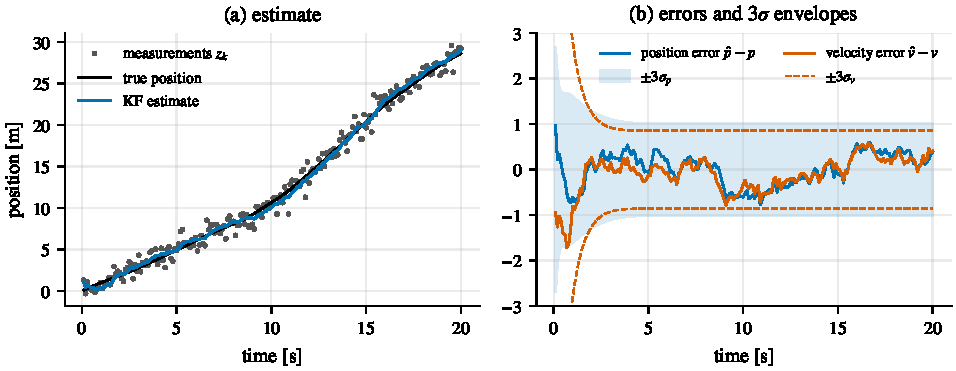
\includegraphics[width=\textwidth]{fig_kf1d.pdf}
  \caption{A constant-velocity Kalman filter tracking a 1D target from noisy position measurements. (a) The estimate smooths the measurements.
  (b) The errors stay inside the $\pm3\sigma$ envelopes, which shrink quickly from the uninformative prior and settle at the steady-state values set by
  the balance between process noise and measurement noise. The velocity is never measured, yet it is estimated through its correlation with
  position.}
  \label{fig:kf1d}
\end{figure}

\Cref{fig:kf1d} shows the filter on the constant-velocity model (\cref{ex:double-integrator-qd}), with position measurements at 10~Hz. Three behaviors
generalize to VIO. The covariance converges from its initial value to a steady state determined only by $Q$, $R$ and the geometry, not by the
data. The unmeasured state (velocity) is estimated through the correlation that the dynamics build up between position and velocity. And the errors
stay inside the $3\sigma$ envelope about 99.7\% of the time, the visual signature of a consistent filter.

\begin{takeaways}
\begin{itemize}
  \item Predict: $\hat x \gets \Phi\hat x$, $P \gets \Phi P\Phi\T + Q$. Update: condition the joint Gaussian of state and measurement.
  \item $K = PH\T S\inv$ maps innovations into state corrections, including corrections to unmeasured but correlated states.
  \item The Kalman filter is the exact Bayesian filter for linear-Gaussian models and the best linear filter otherwise.
  \item Innovations of a correct filter are white with covariance $S$; their NIS is $\chi^2$. This is testable without ground truth.
  \item Time-invariant observable systems reach a steady state set by the balance of process and measurement noise.
  \item Use the Joseph form, solve rather than invert, and symmetrize. Independent measurement blocks may be processed sequentially.
\end{itemize}
\end{takeaways}

\begin{exercises}
  \item Derive \eqref{eq:kf-update} for a scalar state measured twice by independent sensors of variances $R_1$ and $R_2$, first sequentially, then as a
        stacked 2D measurement. Show that the results agree.
  \item Show that $P^+ \preceq P^-$ for the optimal gain. Is this still true for an arbitrary gain in the Joseph form?
  \item Construct a $2\times2$ example in which $(I - KH)P^-$ computed in single precision is not positive semi-definite while the Joseph form is.
  \item Continue the worked example for five more steps and verify that $P_k^-$ converges to 2.
  \item For the scalar random walk with process variance $q$ and measurement variance $r$, derive $P^-_\infty = \tfrac12(q + \sqrt{q^2 + 4qr})$ and the
        steady-state gain. What happens as $q/r \to 0$ and $q/r \to \infty$?
  \item Implement \cref{alg:kf-update} in Python, reproduce \cref{fig:kf1d}, and compute the fraction of time steps where the position error lies outside
        $\pm3\sigma$.
  \item Test the whiteness of the innovations of your filter by computing their sample autocorrelation. Then mis-tune $Q$ and repeat.
\end{exercises}

\chapter{Nonlinear Filtering}
\label{ch:nonlinear}

\begin{objectives}
\begin{itemize}
  \item Derive the extended Kalman filter by linearization, and identify every approximation it makes.
  \item Understand the iterated EKF as Gauss--Newton.
  \item Understand the unscented transform and the unscented Kalman filter.
  \item Understand particle filters and why they do not scale to VIO.
  \item Know why VIO filters are EKFs, and what that implies for how they must be designed.
\end{itemize}
\end{objectives}

Real systems are nonlinear: rotations enter through trigonometric functions, projections divide by depth. A Gaussian pushed through a
nonlinear function is no longer Gaussian (\cref{sec:linearization}), so the exact Bayes filter of \cref{ch:kf} no longer has a finite-dimensional
form. This chapter presents the three main families of approximations. The extended Kalman filter, the basis of this project, is treated in
detail; the others are presented so that the choice is understood.

% ==============================================================================
\section{The extended Kalman filter}

\subsection{The model}

A nonlinear discrete-time model reads
\begin{equation}
  x_k = f(x_{k-1}, u_k, w_k), \qquad z_k = h(x_k) + n_k,
  \label{eq:nonlinear-model}
\end{equation}
with known input $u_k$ (an IMU reading, for instance), process noise $w_k \sim \N(0, Q_k)$ and measurement noise $n_k \sim \N(0, R_k)$.

\subsection{Derivation}

The \term{extended Kalman filter} (EKF) applies the Kalman filter to a linearization of the model about the current estimate.

\paragraph{Prediction.} Expand $f$ to first order around the previous estimate and zero noise:
\begin{equation}
  x_k \approx f(\hat x_{k-1}^+, u_k, 0) + F_k\,(x_{k-1} - \hat x_{k-1}^+) + L_kw_k,
  \qquad F_k = \frac{\partial f}{\partial x}\Big|_{\hat x_{k-1}^+},\quad L_k = \frac{\partial f}{\partial w}\Big|_{\hat x_{k-1}^+} .
\end{equation}
Taking the mean and covariance of the right-hand side (\cref{prop:affine}):
\begin{equation}
  \hat x_k^- = f(\hat x_{k-1}^+, u_k, 0), \qquad P_k^- = F_kP_{k-1}^+F_k\T + L_kQ_kL_k\T .
\end{equation}
The mean is propagated through the \emph{nonlinear} function, the covariance through its Jacobian.

\paragraph{Update.} Expand $h$ around the prediction, $h(x_k) \approx h(\hat x_k^-) + H_k(x_k - \hat x_k^-)$ with $H_k = \partial h/\partial x|_{\hat x_k^-}$, and apply the linear update with
the innovation computed from the nonlinear prediction:
\begin{equation}
\begin{gathered}
  r_k = z_k - h(\hat x_k^-), \qquad S_k = H_kP_k^-H_k\T + R_k, \qquad K_k = P_k^-H_k\T S_k\inv, \\
  \hat x_k^+ = \hat x_k^- + K_kr_k, \qquad P_k^+ = (I - K_kH_k)P_k^-(I - K_kH_k)\T + K_kR_kK_k\T .
\end{gathered}
\end{equation}

\subsection{What the EKF gets wrong}

Every step above is exact for linear models. For nonlinear models the EKF makes three approximations:
\begin{enumerate}
  \item \emph{Gaussianity}: the true prior and posterior are not Gaussian, but are represented by a mean and a covariance.
  \item \emph{Mean bias}: the predicted mean is $f(\hat x)$, not $\E[f(x)]$. By \cref{sec:linearization} the difference is about
        $\tfrac12\sum_ie_i\tr(\nabla^2f_i\,P)$, proportional to the curvature times the covariance.
  \item \emph{Covariance error}: $FPF\T$ ignores higher-order terms, and the Jacobians are evaluated at the \emph{estimate}, not at the unknown true state.
\end{enumerate}
All three errors grow with the size of the uncertainty relative to the scale over which the functions curve. When errors are small, the EKF is
excellent; when they are large, it can be badly wrong, and in particular it can become \emph{inconsistent}: report a covariance smaller than its
actual errors. The third approximation has a subtle long-term consequence in VIO, a spurious gain of information about unobservable directions
(\cref{ch:observability}).

\subsection{The iterated EKF}

By \cref{prop:ekf-gn}, the EKF update is one Gauss--Newton step on the MAP cost $\tfrac12\|x - \hat x^-\|^2_{(P^-)\inv} + \tfrac12\|z - h(x)\|^2_{R\inv}$, linearized at the prior
mean. When the measurement function is strongly nonlinear, that single step can be inaccurate. The \term{iterated EKF} (IEKF) repeats it,
re-linearizing at the latest iterate $x^{(i)}$ while keeping the prior term:
\begin{equation}
  x^{(i+1)} = \hat x^- + K^{(i)}\big(z - h(x^{(i)}) - H^{(i)}(\hat x^- - x^{(i)})\big), \qquad K^{(i)} = P^-H^{(i)\T}\big(H^{(i)}P^-H^{(i)\T} + R\big)\inv,
\end{equation}
with $H^{(i)}$ evaluated at $x^{(i)}$ and $x^{(0)} = \hat x^-$. The first iteration is the EKF. The covariance is computed with the last Jacobian. Iteration
helps when the measurement is very informative relative to the prior, so that the posterior lies far from the prior mean, where the first
linearization is poor.

% ==============================================================================
\section{Sigma-point filters}

\subsection{The unscented transform}

Linearization approximates the \emph{function}. The \term{unscented transform} approximates the \emph{distribution} instead, by a small set of
deterministically chosen \emph{sigma points} that have the right mean and covariance, and pushes each point through the exact nonlinear function.

For $x \in \R^n$ with mean $\mu$ and covariance $P = LL\T$ (Cholesky), choose $\lambda = \alpha^2(n + \kappa) - n$ and the $2n + 1$ points
\begin{equation}
  \chi_0 = \mu, \qquad \chi_i = \mu + \sqrt{n + \lambda}\,\ell_i, \qquad \chi_{n+i} = \mu - \sqrt{n + \lambda}\,\ell_i, \qquad i = 1, \dots, n,
\end{equation}
where $\ell_i$ is the $i$-th column of $L$, with weights
\begin{equation}
  W_0^{(m)} = \frac{\lambda}{n + \lambda}, \quad W_0^{(c)} = \frac{\lambda}{n + \lambda} + (1 - \alpha^2 + \beta), \quad W_i^{(m)} = W_i^{(c)} = \frac{1}{2(n + \lambda)} .
\end{equation}
Propagate $\gamma_i = f(\chi_i)$ and recombine:
\begin{equation}
  \bar y = \sum_iW_i^{(m)}\gamma_i, \qquad P_y = \sum_iW_i^{(c)}(\gamma_i - \bar y)(\gamma_i - \bar y)\T .
\end{equation}
The points are placed symmetrically along the principal axes of the uncertainty, so the weighted points reproduce $\mu$ and $P$ exactly. Expanding $f$
in a Taylor series about $\mu$ shows that $\bar y$ captures the second-order (curvature) term of the mean that linearization misses, and that
$P_y$ is correct to second order, without computing any derivatives. The parameters $\alpha$, $\beta$, $\kappa$ control the spread of the points
($\beta = 2$ is optimal for Gaussians).

\begin{figure}[t]
  \centering
  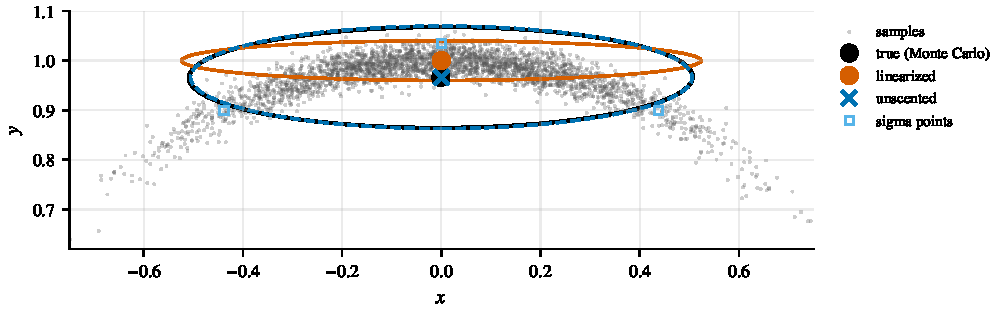
\includegraphics[width=\textwidth]{fig_ut.pdf}
  \caption{A range-bearing measurement converted to Cartesian coordinates, with $\sigma_r = 0.02$ and $\sigma_\phi = 15^\circ$. Monte Carlo samples of the true
  distribution (dots), its true mean and covariance (black), the linearized approximation (orange), and the unscented transform (blue, dashed), with the five
  sigma points; ellipses are $2\sigma$. Linearization places the mean on the circle, where it should not be; the unscented transform recovers the inward shift of the
  mean and a better covariance.}
  \label{fig:ut}
\end{figure}

\subsection{The unscented Kalman filter}

The \emph{unscented Kalman filter} (UKF) uses the unscented transform for both steps. Prediction: generate sigma points from $(\hat x^+, P^+)$, propagate them
through $f$, and recombine into $(\hat x^-, P^-)$, adding $Q$. Update: generate sigma points from $(\hat x^-, P^-)$, push them through $h$ to get the predicted
measurement $\bar z$ and its covariance $S$ (adding $R$), and the cross-covariance $P_{xz} = \sum_iW_i^{(c)}(\chi_i - \hat x^-)(\gamma_i - \bar z)\T$; then
$K = P_{xz}S\inv$, $\hat x^+ = \hat x^- + K(z - \bar z)$ and $P^+ = P^- - KSK\T$. These are the LMMSE formulas of \cref{thm:lmmse} with moments estimated by the
sigma points rather than by linearization. On manifolds, sigma points are generated in the tangent space and mapped with $\bplus$, and their mean is
computed iteratively as in \cref{ch:lie}.

The UKF costs about $2n + 1$ evaluations of $f$ and $h$ per step instead of Jacobians, which is attractive when Jacobians are hard to derive. For VIO
with a 75-dimensional state, the $151$ propagations of the full state per IMU sample are expensive, and the accuracy gain over a well-designed
error-state EKF is small, because the error-state formulation already keeps the nonlinearity mild.

% ==============================================================================
\section{Particle filters}

A \term{particle filter} represents the posterior by $N$ weighted samples (particles) $\{x^{(j)}, w^{(j)}\}$, which can represent any distribution,
multi-modal ones included. The basic \emph{sequential importance resampling} (SIR) algorithm:
\begin{enumerate}
  \item \emph{Predict}: move each particle through the dynamics with a random noise sample, $x_k^{(j)} = f(x_{k-1}^{(j)}, u_k, w^{(j)})$.
  \item \emph{Weight}: multiply each weight by the likelihood of the measurement, $w^{(j)} \gets w^{(j)}p(z_k\mid x_k^{(j)})$, and normalize.
  \item \emph{Resample}: when the effective sample size $N_{\mathrm{eff}} = 1/\sum_j(w^{(j)})^2$ falls too low, draw $N$ new particles with probabilities $w^{(j)}$ and
        reset the weights to $1/N$, so that particles concentrate where the posterior mass is.
\end{enumerate}
Particle filters are exact as $N\to\infty$ and excel at low-dimensional problems with multi-modal posteriors, such as localizing a robot in a known
map. Their weakness is dimension: the number of particles needed to cover a distribution grows roughly exponentially with the state dimension.
For the 15 to 75 dimensions of VIO they are impractical, except in hybrid forms that sample only a few variables.

% ==============================================================================
\section{Why VIO uses the EKF}

\begin{center}\small
\begin{tabularx}{\textwidth}{@{}>{\raggedright\arraybackslash}p{0.2\textwidth}>{\raggedright\arraybackslash}X>{\raggedright\arraybackslash}X>{\raggedright\arraybackslash}X@{}}
\toprule
 & EKF & UKF & particle filter \\
\midrule
cost per step & Jacobians, $\mathcal{O}(n^3)$ & $2n + 1$ propagations, $\mathcal{O}(n^3)$ & $N$ propagations, $N$ huge for large $n$ \\
derivatives needed & yes & no & no \\
non-Gaussian posteriors & no & no & yes \\
accuracy for small errors & excellent & excellent & good (noisy) \\
used in VIO & MSCKF, OpenVINS, ROVIO (iterated) & rarely & no \\
\bottomrule
\end{tabularx}
\end{center}

Visual-inertial odometry has a high-dimensional state, a fast prediction rate (hundreds of Hz), and uncertainties that, once the filter is initialized,
are small compared with the curvature of its models. Those are exactly the conditions under which the EKF is accurate and the alternatives are
expensive. The design principle that makes this work is to keep the linearized errors small: estimate the \emph{error} of a nominal state that
absorbs the large nonlinear motion, and reset it after every correction. That is the error-state Kalman filter of the next chapter.

\begin{takeaways}
\begin{itemize}
  \item The EKF propagates the mean through the nonlinear model and the covariance through its Jacobians, evaluated at the estimate.
  \item Its errors (non-Gaussianity, mean bias, covariance error, estimate-dependent Jacobians) grow with uncertainty relative to curvature.
  \item The iterated EKF is Gauss--Newton on the MAP cost; it helps when measurements are very informative.
  \item The unscented transform propagates sigma points through the exact function and captures second-order effects without derivatives.
  \item Particle filters handle any distribution but scale exponentially with dimension.
  \item VIO uses EKFs with small, frequently reset errors: the error-state formulation.
\end{itemize}
\end{takeaways}

\begin{exercises}
  \item Write the EKF for a planar robot with state $(x, y, \psi)$ driven by speed and turn rate and measured by range to a known beacon. Identify where
        linearization error enters.
  \item Reproduce \cref{fig:ut}. Increase $\sigma_\phi$ until the linearized mean lies outside the $1\sigma$ ellipse of the true distribution.
  \item Show that the unscented transform reproduces the mean and covariance exactly for a linear function.
  \item Show that for a scalar $x \sim \N(\mu, \sigma^2)$ and $f(x) = x^2$, the unscented transform with $n = 1$, $\kappa = 2$, $\alpha = 1$ gives the exact mean $\mu^2 + \sigma^2$.
  \item Implement a particle filter for a 1D robot localizing itself from range measurements to two landmarks, and observe a bimodal posterior.
\end{exercises}
% Solutions to the exercises of Chapter 13.
\begin{solutions}
  \item State $x = (p_x, p_y, \psi)$, inputs $(v, \omega)$ with noise $(n_v, n_\omega)$, beacon at $b = (b_x, b_y)$ with known position.
        \begin{itemize}[leftmargin=1.2em]
          \item \emph{Prediction}: $f(x) = \big(p_x + v\Dt\cos\psi,\ p_y + v\Dt\sin\psi,\ \psi + \omega\Dt\big)$, with Jacobians
                \[
                  F = \begin{bmatrix}1 & 0 & -v\Dt\sin\hat\psi\\ 0 & 1 & v\Dt\cos\hat\psi\\ 0 & 0 & 1\end{bmatrix}, \qquad
                  L = \begin{bmatrix}\Dt\cos\hat\psi & 0\\ \Dt\sin\hat\psi & 0\\ 0 & \Dt\end{bmatrix},
                \]
                and $P^- = FPF\T + L\diag(\sigma_v^2, \sigma_\omega^2)L\T$.
          \item \emph{Update}: $h(x) = \rho = \|p - b\|$, $H = \big[(\hat p_x - b_x)/\hat\rho,\ (\hat p_y - b_y)/\hat\rho,\ 0\big]$, then the standard update.
        \end{itemize}
        Linearization error enters in three places. (i) In the prediction through $\cos\psi$ and $\sin\psi$: with a large heading uncertainty the predicted
        positions spread along an arc, the banana of \cref{fig:banana}, which $FPF\T$ approximates by an ellipse. (ii) In the update through the curvature of the
        range: $\nabla^2h$ has the eigenvalue $1/\rho$ in the direction perpendicular to the line of sight, so the neglected second-order term is about
        $\sigma_\perp^2/(2\rho)$, harmless far from the beacon and large close to it (and $H$ is undefined at $\rho = 0$). (iii) In the heading: the range does not
        depend on $\psi$ ($H_\psi = 0$), so the heading is corrected only through the position-heading correlation that motion builds in $P$, which is
        itself a linearized quantity. When the heading error is large, those correlations are wrong and the corrections are too.

  \item With the figure's $\sigma_r = 0.02$, the true distribution of $(x, y) = (r\cos\phi, r\sin\phi)$ for $\phi \sim \N(\pi/2, \sigma_\phi^2)$ has mean $(0, e^{-\sigma_\phi^2/2})$ and
        $\Var(y) = (1 + \sigma_r^2)(1 + e^{-2\sigma_\phi^2})/2 - e^{-\sigma_\phi^2}$, while linearization predicts the mean $(0, 1)$. The covariance is diagonal by symmetry,
        so the Mahalanobis distance of the linearized mean is $d = (1 - e^{-\sigma_\phi^2/2})/\sqrt{\Var(y)}$:
        \begin{center}\small
        \begin{tabular}{@{}l c c c c c c@{}}
        \toprule
        $\sigma_\phi$ & $15^\circ$ & $30^\circ$ & $45^\circ$ & $60^\circ$ & $75^\circ$ & $90^\circ$ \\
        \midrule
        $d$ & 0.67 & 0.75 & 0.81 & 0.90 & 0.99 & 1.10 \\
        \bottomrule
        \end{tabular}
        \end{center}
        The linearized mean leaves the $1\sigma$ ellipse at $\sigma_\phi \approx 76^\circ$ (confirmed by Monte Carlo). Notice that it never gets very far: in the
        small-angle regime $d^2 \approx (\sigma_\phi^4/4)/(\sigma_r^2 + \sigma_\phi^4/2) < \tfrac12$, because the true distribution spreads along the arc as fast as its mean moves
        inward. The more telling failure is the shape: the true distribution is a thin curved arc, and the linearized ellipse puts most of its
        probability where the true one has none.

  \item For $f(x) = Ax + b$ the transformed sigma points are $y_0 = A\mu + b$ and $y_{i}, y_{n+i} = A\mu + b \pm\sqrt{n + \lambda}\,A\ell_i$. The mean weights sum to
        one ($\frac{\lambda}{n + \lambda} + \frac{2n}{2(n + \lambda)} = 1$) and the $\pm$ pairs cancel, so $\bar y = \sum_iW_i^{(m)}y_i = A\mu + b$. In the covariance the central point
        contributes nothing ($y_0 - \bar y = 0$, so the value of $W_0^{(c)}$ and of $\beta$ is irrelevant), and each pair contributes
        $2\cdot\frac{1}{2(n + \lambda)}(n + \lambda)A\ell_i\ell_i\T A\T$:
        \[
          \sum_iW_i^{(c)}(y_i - \bar y)(y_i - \bar y)\T = A\Big(\sum_{i=1}^n\ell_i\ell_i\T\Big)A\T = ALL\T A\T = APA\T .
        \]
        The unscented transform is exact for linear functions, as it must be to be consistent with the Kalman filter.

  \item With $n = 1$, $\kappa = 2$ and $\alpha = 1$: $\lambda = 1\cdot3 - 1 = 2$, $n + \lambda = 3$, sigma points $\mu$ and $\mu \pm \sqrt3\,\sigma$, weights $W_0^{(m)} = \tfrac23$ and
        $W_{1,2}^{(m)} = \tfrac16$. For $f(x) = x^2$,
        \[
          \tfrac23\mu^2 + \tfrac16\big((\mu + \sqrt3\sigma)^2 + (\mu - \sqrt3\sigma)^2\big) = \tfrac23\mu^2 + \tfrac16\big(2\mu^2 + 6\sigma^2\big) = \mu^2 + \sigma^2 = \E[x^2],
        \]
        exactly, whereas linearization gives $\mu^2$. (The choice $\kappa = 3 - n$ also makes the sigma points reproduce the fourth moment $3\sigma^4$ of a scalar
        Gaussian: $\tfrac16\cdot2\cdot9\sigma^4 = 3\sigma^4$.)

  \item A simple model that produces bimodality: landmarks at $0$ and $10$ on a line, and a sensor that reports the range to the \emph{nearest} landmark
        without saying which one it is ($z = \min(|x|, |x - 10|) + n$, $\sigma_z = 0.1$). The robot starts at $x = 2$ with a uniform prior on $[0, 10]$ and
        then moves right by $0.5$ per step (odometry noise $0.05$). A bootstrap particle filter with 2000 particles: propagate each particle with the
        odometry plus sampled noise, multiply its weight by the likelihood $\exp(-(z - h(x_i))^2/2\sigma_z^2)$, normalize, and resample when the effective
        sample size $1/\sum_iw_i^2$ drops below $N/2$. After the first measurement ($z = 1.87$) the posterior has two equal modes, near $1.9$ and near $8.1$
        (weights $0.52$ and $0.48$), symmetric about $5$; its mean, $4.9$, is a place where the robot certainly is not, which is what a Gaussian filter
        would report. After the first move the mirror hypothesis predicts a range of about $1.4$ (it approaches the landmark at 10) while the
        measurement says $2.3$; its weight drops to zero and the filter tracks the true position from then on. A Kalman-type filter cannot represent
        the bimodal stage at all: it would either lock onto one mode, possibly the wrong one, or average them.
\end{solutions}


\chapter{The Error-State Kalman Filter}
\label{ch:eskf}

\begin{objectives}
\begin{itemize}
  \item Understand the three-way split into true, nominal and error state, and why it is the right way to filter on a manifold.
  \item Derive the linearized error dynamics with a mechanical recipe.
  \item Define measurement residuals and Jacobians on the manifold with the correct sign convention.
  \item Derive the injection and reset steps, including the reset Jacobian $G$.
  \item Assemble the complete error-state Kalman filter loop, and follow it through a complete attitude-estimation example.
\end{itemize}
\end{objectives}

% ==============================================================================
\section{Filtering on a manifold}

The EKF of \cref{ch:nonlinear} assumes the state lives in $\R^n$, so that $\hat x + Kr$ makes sense. For VIO, the state contains a rotation, which does
not live in a vector space (\cref{ch:lie}). Three quantities must therefore be distinguished.

\begin{definition}[True, nominal and error state]
\index{error state}\index{nominal state}
\begin{itemize}
  \item The \textbf{true state} $x$ is the unknown physical state, a point on the state manifold $\mathcal{M}$.
  \item The \textbf{nominal state} $\hat x \in \mathcal{M}$ is the current best estimate, propagated with the full nonlinear model and no noise.
  \item The \textbf{error state} $\delta x = x \bminus \hat x \in \R^{n}$ is the small, minimal-dimension difference, defined with the operators of
        \cref{sec:boxplus}.
\end{itemize}
The filter's Gaussian belief is over the error state: $\delta x \sim \N(\delta\hat x, P)$, so that $x = \hat x \bplus \delta x$.
\end{definition}

For the IMU state this means 16 nominal numbers (quaternion included) but a 15-dimensional error and a $15\times15$ covariance, with no redundant
directions and no constraints. The Kalman filter operates only on the error state, which is a vector, so all of \cref{ch:kf} applies to it. This
design is called the \term{error-state Kalman filter} (ESKF), or \emph{indirect} Kalman filter. In aerospace the same idea for attitude is the
\emph{multiplicative} EKF.

\begin{keyidea}[why the error state]
\begin{itemize}
  \item \textbf{Minimal and unconstrained.} The error has exactly as many components as degrees of freedom, so its covariance is non-singular and
        needs no constraint handling.
  \item \textbf{Always near the origin.} After every update the error is reset to zero, so it never approaches the singularities of
        three-parameter rotations, and the small-angle approximations used to derive its dynamics remain valid.
  \item \textbf{Nearly linear.} The large, fast, nonlinear motion is carried by the nominal state, which is integrated exactly. The error evolves
        slowly and is small, so its dynamics are almost linear and linearization is accurate (\cref{ch:nonlinear}).
  \item \textbf{Slow.} Error dynamics are governed by sensor errors, not by vehicle motion, so the covariance could even be propagated at a lower rate
        than the nominal state if computation were scarce.
\end{itemize}
\end{keyidea}

% ==============================================================================
\section{The ESKF cycle}

\begin{figure}[t]
\centering
\begin{tikzpicture}[node distance=14mm and 30mm]
  \node[block, minimum width=40mm] (nom) {\textbf{1. Nominal propagation}\\ $\hat x \gets f(\hat x, u)$, noise-free, nonlinear};
  \node[block, minimum width=40mm, right=of nom] (cov) {\textbf{2. Covariance propagation}\\ $P \gets \Phi P\Phi\T + Q_d$};
  \node[block, minimum width=40mm, below=of cov] (upd) {\textbf{3. Update}\\ $r = z\bminus h(\hat x)$, \ $\delta\hat x = Kr$\\ $P \gets$ Joseph form};
  \node[block, minimum width=40mm, below=of nom] (inj) {\textbf{4. Inject and reset}\\ $\hat x \gets \hat x\bplus\delta\hat x$, \ $\delta\hat x \gets 0$\\ $P \gets GPG\T$};
  \draw[->, thick] (nom) -- node[note, above]{every IMU} node[note, below]{sample} (cov);
  \draw[->, thick] (cov) -- node[note, right, align=left]{measurement\\arrives} (upd);
  \draw[->, thick] (upd) -- (inj);
  \draw[->, thick] (inj) -- (nom);
  \draw[->, thick, dashed] (cov.north) to[out=135, in=45] node[note, above]{no measurement: next IMU sample} (nom.north);
\end{tikzpicture}
\caption{The error-state Kalman filter cycle. The error-state mean is zero throughout propagation, so only the covariance is propagated in step 2. It
becomes non-zero in step 3 and is transferred to the nominal state and zeroed in step 4.}
\label{fig:eskf-cycle}
\end{figure}

\Cref{fig:eskf-cycle} shows the four steps.
\begin{enumerate}
  \item \textbf{Nominal propagation.} At each IMU sample, integrate the nonlinear kinematics with the measured inputs, ignoring noise
        (\cref{ch:strapdown}).
  \item \textbf{Error covariance propagation.} Propagate $P$ with the linearized error dynamics (\cref{ch:errordyn}).
  \item \textbf{Update.} When a measurement arrives, compute the residual and its Jacobian on the manifold, and compute the Kalman estimate of the
        error, $\delta\hat x = Kr$, and the posterior covariance.
  \item \textbf{Injection and reset.} Move the estimated error into the nominal state with $\bplus$, set the error mean back to zero, and correct the
        covariance for the change of reference point.
\end{enumerate}

\begin{proposition}[The error mean needs no propagation]
If $\delta\hat x = 0$ after a reset, and the error obeys linear dynamics $\dot{\delta x} = F_c\delta x + G_cw$ with zero-mean noise, then $\E[\delta x] = 0$ until the
next update.
\end{proposition}
\begin{proof}
The mean obeys $\frac{\dd}{\dd t}\E[\delta x] = F_c\,\E[\delta x]$ (\cref{prop:lyapunov}) with initial value zero, whose unique solution is zero.
\end{proof}

This is why step 2 propagates only the covariance: all the knowledge of the error state's mean has been transferred into the nominal state.

% ==============================================================================
\section{Linearized error dynamics: the recipe}
\label{sec:error-dyn-recipe}

Suppose the true state obeys $\dot x = f(x, u, w)$ with noise $w$, and the nominal state obeys $\dot{\hat x} = f(\hat x, u, 0)$. The error dynamics are
derived in four mechanical steps.
\begin{enumerate}
  \item Write the true dynamics block by block.
  \item Substitute $x = \hat x\bplus\delta x$ in every block. For the attitude, $R = \hat R\Exp(\delta\theta)$ (or $\Exp(\delta\theta)\hat R$ for a global perturbation).
  \item Subtract the nominal dynamics.
  \item Keep only terms of first order in the small quantities ($\delta x$ and $w$), using $\Exp(\delta\theta) \approx I + \sx{\delta\theta}$ and dropping their
        products.
\end{enumerate}
The result is a linear time-varying system
\begin{equation}
  \dot{\delta x} = F_c(\hat x, u)\,\delta x + G_c(\hat x)\,w,
\end{equation}
which \cref{sec:discretization} turns into $\Phi$ and $Q_d$. The attitude block needs the time derivative of the perturbation itself, worked out in
\cref{lem:dexp}. \Cref{sec:ahrs} applies the recipe to a complete small filter, and \cref{ch:errordyn} to the inertial navigation equations.

% ==============================================================================
\section{Measurement updates on the manifold}
\label{sec:manifold-update}

Let a sensor produce a measurement $z$ on a manifold $\mathcal{Z}$ (a vector space, $\SO$, a pose, \dots) according to the generative model
\begin{equation}
  z = h(x)\bplus n, \qquad n \sim \N(0, R_z).
\end{equation}
The ESKF compares the measurement with its prediction from the nominal state,
\begin{equation}
  r = z \bminus h(\hat x),
  \label{eq:manifold-residual}
\end{equation}
and models how the residual depends on the unknown true error $\delta x$. Substituting $z = h(\hat x\bplus\delta x)\bplus n$ and linearizing,
\begin{equation}
  r \approx H\,\delta x + n, \qquad
  H = \frac{\partial}{\partial\delta x}\Big[ h(\hat x\bplus\delta x)\bminus h(\hat x) \Big]_{\delta x = 0}.
  \label{eq:manifold-H}
\end{equation}
$H$ is the manifold Jacobian of $h$ (\cref{def:manifold-jacobian}). With $r$ and $H$, the update is the ordinary Kalman update of the error state
with prior $\N(0, P)$:
\begin{equation}
  S = HPH\T + R_z,\qquad K = PH\T S\inv,\qquad \delta\hat x = Kr,\qquad P^+ = (I - KH)P(I - KH)\T + KR_zK\T.
\end{equation}

\begin{pitfall}[the sign of $H$]
There are two ways to set up the linearization, and they differ by a sign. The generative view above differentiates the \emph{prediction} with
respect to the \emph{true} error: $r \approx +H\delta x$. An optimization view instead writes the residual as a function of a correction $\delta$ to the
estimate, $e(\delta) = z\bminus h(\hat x\bplus\delta)$, whose Jacobian is $-H$ (to first order). Both lead to the same correction if used consistently.
Mixing them flips every correction. In this project, $H$ is always \eqref{eq:manifold-H}, and its finite-difference test perturbs the nominal state:
$r(\delta x) := h(\hat x\bplus\delta x)\bminus h(\hat x)$ and $H \approx \partial r/\partial\delta x$.
\end{pitfall}

For a vector-valued measurement, $\bminus$ is subtraction and this reduces to the EKF. For a rotation-valued measurement such as the pose
measurement of Milestone 6, the attitude part of the residual is $\Log_q(\hat q\inv\qprod q_{meas})$ (AGENTS.md F3).

% ==============================================================================
\section{Injection and reset}
\label{sec:reset}

After the update, the error estimate $\delta\hat x = Kr$ is non-zero. Injection moves it into the nominal state:
\begin{equation}
  \hat x^+ = \hat x\bplus\delta\hat x:\quad
  \hat p \gets \hat p + \delta\hat p,\quad \hat v \gets \hat v + \delta\hat v,\quad
  \hat q \gets \hat q\qprod\Exp_q(\delta\hat\theta),\quad \hat b \gets \hat b + \delta\hat b,
\end{equation}
followed by normalization of every quaternion that was touched, for the IMU and every clone (AGENTS.md F4).

The error is now defined relative to the new nominal state, $\delta x^+ = x\bminus\hat x^+$, and its mean is zero. But its covariance is not exactly $P^+$,
because the reference point of the tangent space has moved.

\begin{proposition}[Reset Jacobian]
\label{prop:reset}
\index{reset Jacobian}
Let $\delta x \sim \N(\delta\hat x, P^+)$ be the error relative to $\hat x$ after the update, and $\delta x^+ = x\bminus(\hat x\bplus\delta\hat x)$ the error relative to the
injected nominal state. To first order, $\delta x^+ \sim \N(0, GP^+G\T)$ with $G = \partial\delta x^+/\partial\delta x$ evaluated at $\delta\hat x$. For the vector blocks
$G = I$, and for each attitude block
\begin{equation}
  G_\theta = I - \tfrac12\sx{\delta\hat\theta}.
  \label{eq:reset-G}
\end{equation}
\end{proposition}
\begin{proof}
For vector blocks $\delta x^+ = \delta x - \delta\hat x$, whose Jacobian is $I$. For the attitude, $q = \hat q\qprod\Exp_q(\delta\theta)$ and
$q = \hat q^+\qprod\Exp_q(\delta\theta^+)$ with $\hat q^+ = \hat q\qprod\Exp_q(\delta\hat\theta)$, so
\begin{equation*}
  \Exp(\delta\theta^+) = \Exp(-\delta\hat\theta)\,\Exp(\delta\theta).
\end{equation*}
By the BCH formula \eqref{eq:bch}, $\delta\theta^+ = \delta\theta - \delta\hat\theta - \tfrac12\,\delta\hat\theta\times\delta\theta + \cdots$, whose derivative with respect to $\delta\theta$ is
$I - \tfrac12\sx{\delta\hat\theta}$. At $\delta\theta = \delta\hat\theta$ the value is exactly zero, so the new error has zero mean. Linearizing $\delta x^+$ about $\delta\hat x$ and applying
\cref{prop:affine} gives the covariance.
\end{proof}

\begin{remark}[relation to the right Jacobian]
The derivative of $\Log(\Exp(-\delta\hat\theta)\Exp(\delta\theta))$ at $\delta\theta = \delta\hat\theta$ can be computed exactly with \eqref{eq:jr-def}: it is
$\Jr(\delta\hat\theta) = I - \tfrac12\sx{\delta\hat\theta} + O(\|\delta\hat\theta\|^2)$. The frozen specification (AGENTS.md F4) uses the first-order form \eqref{eq:reset-G}. For a
typical correction of a few milliradians the two differ by about $10^{-6}$ and the difference is irrelevant. Changing it would be a logged
convention change, not a silent substitution.
\end{remark}

The covariance reset is therefore
\begin{equation}
  P \gets G P G\T, \qquad G = \blkdiag\big(I_6,\ I - \tfrac12\sx{\delta\hat\theta},\ I_6,\ \ldots\big),
\end{equation}
with one $I - \tfrac12\sx{\delta\hat\theta_i}$ block for each clone's attitude and identity elsewhere.

\begin{convention}[injection and reset, AGENTS.md F4]
Inject with $\bplus$ into the IMU block and every clone; normalize every touched quaternion; reset $\delta\hat x \gets 0$ and $P \gets GPG\T$ with $G$
implemented exactly as above. Using $G \approx I$ is a deviation that must be logged.
\end{convention}

How much does $G$ matter? It rotates the attitude covariance by half the injected correction, a first-order effect in $\|\delta\hat\theta\|$. With small
corrections at high rate the effect is tiny, and many implementations use $G = I$. Large corrections (after a long outage, or a loop closure) make it
noticeable. It costs almost nothing, and implementing it exactly removes one approximation from the consistency analysis of Milestone 7.

% ==============================================================================
\section{The complete error-state filter}

\begin{algorithm}[t]
\caption{Error-state Kalman filter (one IMU step and an optional update)}
\label{alg:eskf}
\begin{algorithmic}[1]
\Require nominal $\hat x$, covariance $P$, IMU sample at $t_k$, optional measurement $z$ at $t_k$
\State $\Dt \gets t_k - t_{k-1}$ \Comment{from integer nanosecond timestamps}
\State $\hat x \gets f(\hat x, u_k, \Dt)$; normalize $\hat q$ \Comment{nominal propagation}
\State $\Phi \gets I + F_c\Dt$; \quad $Q_d \gets G_cQ_cG_c\T\Dt$
\State $P \gets \Phi P\Phi\T + Q_d$; \quad $P \gets \tfrac12(P + P\T)$
\If{measurement $z$ available}
  \State $r \gets z\bminus h(\hat x)$; \quad $H \gets \partial[h(\hat x\bplus\delta x)\bminus h(\hat x)]/\partial\delta x$
  \State $S \gets HPH\T + R_z$; factor $S$; gate on $r\T S\inv r$
  \State $K \gets PH\T S\inv$ (by solving); \quad $\delta\hat x \gets Kr$
  \State $P \gets (I-KH)P(I-KH)\T + KR_zK\T$
  \State $\hat x \gets \hat x\bplus\delta\hat x$; normalize quaternions \Comment{inject}
  \State $P \gets GPG\T$; \quad $P \gets \tfrac12(P + P\T)$ \Comment{reset}
\EndIf
\end{algorithmic}
\end{algorithm}

\Cref{alg:eskf} assembles the pieces. It is generic: \cref{ch:strapdown,ch:errordyn} supply $f$, $F_c$ and $G_c$ for the IMU, \cref{ch:updates} supplies $h$ and $H$ for a
pose sensor, and \cref{ch:msckfupdate} supplies them for a camera. When measurements arrive between IMU samples, the filter first propagates to the
measurement time by splitting the IMU interval (\cref{ch:strapdown}).

% ==============================================================================
\section{A complete example: attitude estimation}
\label{sec:ahrs}

\index{attitude estimation}
To see every step of \cref{alg:eskf} at work on a problem small enough to follow completely, consider an \emph{attitude and heading reference system}
(AHRS) without a magnetometer: estimate the attitude $R = R_{wb}$ of a slowly moving device and the bias $b$ of its gyroscope, using the gyroscope for
propagation and the accelerometer as an inclinometer (it measures the reaction to gravity when linear accelerations are small).

To avoid solving the project's own derivation exercise, this example uses the \textbf{global} perturbation $R = \Exp(\delta\theta)\hat R$, with the error
expressed in the world frame. The project's state uses the local perturbation; its forms are the subject of the derivation exercises of \cref{ch:errordyn}\ifsolutions{}
(solutions in \cref{app:solutions})\fi.

\paragraph{State and error state.} Nominal $(\hat R, \hat b)$; error $\delta x = (\delta\theta, \delta b) \in \R^6$ with $R = \Exp(\delta\theta)\hat R$ and $b = \hat b + \delta b$.

\paragraph{Models.} Gyroscope $\omega_m = \omega + b + n_g$; bias random walk $\dot b = n_b$; accelerometer at rest $a_m = R\T v + n_a$ with $v = -g_w = (0, 0, 9.81)$.

\paragraph{Nominal propagation.} $\hat R \gets \hat R\Exp\big((\omega_m - \hat b)\Dt\big)$, $\hat b$ unchanged.

\paragraph{Error dynamics.} By \cref{ex:global-attitude} (in \cref{ch:errordyn}), $\dot{\delta\theta} = -\hat R\,\delta b - \hat R\,n_g$, and $\dot{\delta b} = n_b$. Hence
\begin{equation}
  F_c = \begin{bmatrix} 0 & -\hat R \\ 0 & 0\end{bmatrix}, \qquad G_c = \begin{bmatrix} -\hat R & 0 \\ 0 & I\end{bmatrix}, \qquad Q_c = \diag(\sigma_g^2I, \sigma_b^2I).
\end{equation}

\paragraph{Measurement Jacobian.} $h(x) = R\T v$. Perturbing, $h(\Exp(\delta\theta)\hat R) = \hat R\T\Exp(-\delta\theta)v \approx \hat R\T(v - \delta\theta\times v) = \hat R\T v + \hat R\T\sx{v}\,\delta\theta$, so
\begin{equation}
  H = \begin{bmatrix} \hat R\T\sx{v} & 0 \end{bmatrix}, \qquad r = a_m - \hat R\T v .
\end{equation}
$\sx{v}$ has rank two: the measurement observes the two components of $\delta\theta$ perpendicular to gravity (roll and pitch) but not the component along it
(yaw). It does not observe the bias directly at all.

\paragraph{Injection and reset.} $\hat R \gets \Exp(\delta\hat\theta)\hat R$, $\hat b \gets \hat b + \delta\hat b$. Repeating the reset derivation for the global perturbation,
$\Exp(\delta\theta^+) = \Exp(\delta\theta)\Exp(-\delta\hat\theta)$, gives $G_\theta = I + \tfrac12\sx{\delta\hat\theta}$: the same magnitude as \eqref{eq:reset-G}, opposite sign.

\begin{figure}[t]
  \centering
  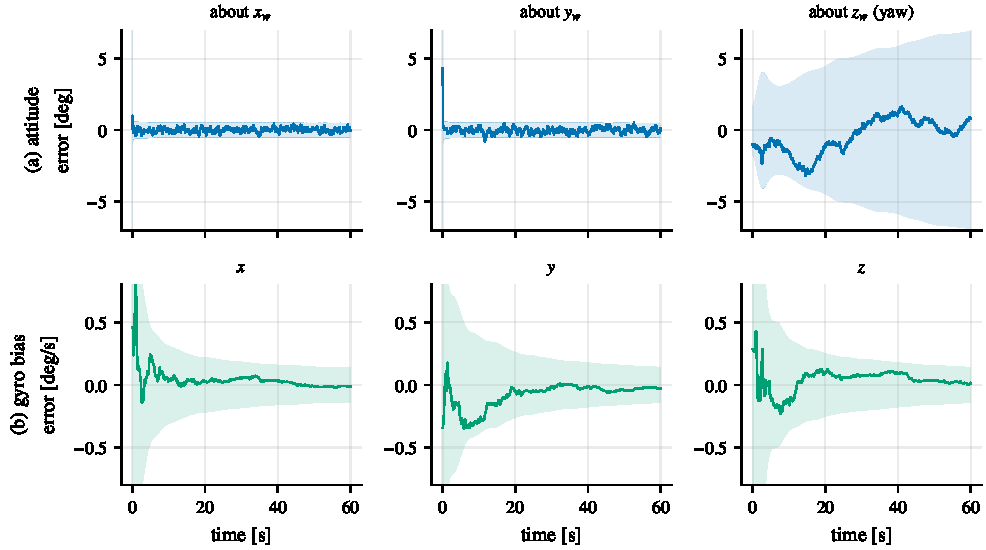
\includegraphics[width=\textwidth]{fig_ahrs.pdf}
  \caption{The attitude ESKF of \cref{sec:ahrs} on a simulated tumbling device: gyroscope at 100~Hz with a constant bias, accelerometer used as an
  inclinometer at 10~Hz. (a) Attitude errors about the world axes with their $\pm3\sigma$ bounds. Tilt (about $x$ and $y$) is quickly bounded by the
  accelerometer; the error about the vertical (yaw) is unobservable, and its bound grows. (b) Gyro bias errors with $\pm3\sigma$ bounds. The bias
  is never measured directly, yet all three components converge, because the device's rotation makes each body axis horizontal at some time.}
  \label{fig:ahrs}
\end{figure}

\Cref{fig:ahrs} shows the filter on simulated data. Several lessons of this chapter are visible in it. The errors stay inside their $3\sigma$
bounds: the filter is consistent. Tilt becomes accurate within seconds, through the accelerometer. Yaw is unobservable without a magnetometer
or vision, so its uncertainty only grows. And the gyro bias, although never measured, is estimated through its correlation with the tilt error
it causes: the cross-covariance built by propagation lets the gain correct it. This is exactly how the full VIO filter estimates IMU biases from
camera measurements.

\begin{projectlink}[Milestones 4--6]
M4 implements step 2 of \cref{alg:eskf}, M5 steps 3--4, and M6 the update, injection and reset with a pose measurement. Testing them separately
localizes bugs: if propagation is exact on synthetic data, and the covariance matches Monte Carlo statistics, then any later inconsistency is in
the update.
\end{projectlink}

\begin{takeaways}
\begin{itemize}
  \item The ESKF splits the state into a nonlinear nominal part and a small, minimal, nearly linear error part. The Kalman filter only ever sees the
        error.
  \item The error mean is zero during propagation; only $P$ is propagated.
  \item Residual $r = z\bminus h(\hat x) \approx H\delta x + n$ with $H$ the manifold Jacobian of $h$ at $\hat x$.
  \item After injection, reset $P \gets GPG\T$ with $G_\theta = I - \tfrac12\sx{\delta\hat\theta}$ for every (local) attitude block.
  \item The attitude example shows observability at work: gravity bounds tilt, yaw drifts, and unmeasured biases are estimated through
        correlations.
\end{itemize}
\end{takeaways}

\begin{exercises}
  \item Derive the reset Jacobian for the global perturbation $R = \Exp(\delta\theta)\hat R$ and confirm $G_\theta = I + \tfrac12\sx{\delta\hat\theta}$.
  \item Suppose $\delta\hat\theta = (0, 0, 0.1)$~rad and $P_{\theta\theta} = \diag(10^{-4}, 10^{-4}, 10^{-2})$. Compute $GP_{\theta\theta}G\T$ and compare with
        $\Jr(\delta\hat\theta)P_{\theta\theta}\Jr(\delta\hat\theta)\T$. When is the difference noticeable?
  \item An iterated ESKF repeats the update with $H$ re-evaluated at $\hat x\bplus\delta\hat x$. Show that one iteration is a Gauss--Newton step on the MAP cost
        $\|\delta x\|^2_{P\inv} + \|z\bminus h(\hat x\bplus\delta x)\|^2_{R_z\inv}$.
  \item Implement the attitude filter of \cref{sec:ahrs} and reproduce \cref{fig:ahrs}. Then hold the device still and observe which bias component stops
        converging. Explain why.
  \item Rewrite the attitude filter with the local perturbation $R = \hat R\Exp(\delta\theta)$: derive $F_c$, $G_c$, $H$ and $G$. (This is a small version of the project's
        derivation exercise.)
\end{exercises}
% Solutions to the exercises of Chapter 14.
\begin{solutions}
  \item With the global perturbation the true attitude is $R = \Exp(\delta\theta)\hat R$ before injection and $R = \Exp(\delta\theta^+)\hat R^+$ after it, with
        $\hat R^+ = \Exp(\delta\hat\theta)\hat R$. Equating, $\Exp(\delta\theta^+) = \Exp(\delta\theta)\Exp(-\delta\hat\theta)$, and the BCH formula \eqref{eq:bch} gives
        \[
          \delta\theta^+ = \delta\theta - \delta\hat\theta - \tfrac12\,\delta\theta\times\delta\hat\theta + \cdots = \delta\theta - \delta\hat\theta + \tfrac12\,\delta\hat\theta\times\delta\theta + \cdots,
        \]
        whose derivative with respect to $\delta\theta$ is $G_\theta = I + \tfrac12\sx{\delta\hat\theta}$. The sign is opposite to the local case
        (\cref{prop:reset}), because the correction now multiplies on the left. (Exactly, the derivative at $\delta\theta = \delta\hat\theta$ is $\Jl(\delta\hat\theta)$.)

  \item Here $\sx{\delta\hat\theta}$ mixes only $x$ and $y$, and $P_{\theta\theta}$ is isotropic in that plane, so both products stay diagonal:
        \begin{align*}
          GP_{\theta\theta}G\T &= \diag\big(1.0025,\ 1.0025,\ 100\big)\times10^{-4}, \\
          \Jr P_{\theta\theta}\Jr\T &= \diag\big(0.9992,\ 0.9992,\ 100\big)\times10^{-4}.
        \end{align*}
        The difference, $0.33\%$ of the $x$ and $y$ variances, is second order: $G$ and $\Jr(\delta\hat\theta) = I - \tfrac12\sx{\delta\hat\theta} + O(\|\delta\hat\theta\|^2)$ agree to
        first order, and their products differ by about $\|\delta\hat\theta\|^2/3$. For anisotropic covariances the first-order rotation of the covariance is the
        same in both, and the relative difference is about $3\times10^{-6}$, $3\times10^{-4}$, $3\%$ and $40\%$ for corrections of $0.003$, $0.03$, $0.3$ and $1$~rad. It
        is negligible for the milliradian corrections of a running filter and noticeable only after very large corrections, such as the first updates
        after a poor initialization.

  \item Let $\delta x$ be the error-state variable with prior $\N(0, P)$ in the tangent space at $\hat x$, and $r(\delta x) = z\bminus h(\hat x\bplus\delta x)$, so that the MAP
        cost is $F(\delta x) = \|\delta x\|^2_{P\inv} + \|r(\delta x)\|^2_{R_z\inv}$. Near an iterate $\delta x_i$, $r(\delta x) \approx r_i - H_i(\delta x - \delta x_i)$ with $r_i = r(\delta x_i)$ and $H_i$ the
        manifold Jacobian of $h$ at $\hat x\bplus\delta x_i$. Minimizing the resulting quadratic gives the Gauss--Newton iterate (the algebra of Exercise 10.7 with
        $\mu = 0$)
        \[
          \delta x_{i+1} = K_i\big(r_i + H_i\,\delta x_i\big), \qquad K_i = PH_i\T\big(H_iPH_i\T + R_z\big)\inv .
        \]
        From $\delta x_0 = 0$ the first iterate is $\delta x_1 = K_0r(0)$ with $H_0$ evaluated at $\hat x$: exactly the ESKF update $\delta\hat x = Kr$. One ESKF update is
        therefore one Gauss--Newton step on the MAP cost; the iterated ESKF re-evaluates $h$ and $H$ at $\hat x\bplus\delta x_i$ and repeats, then injects the final
        $\delta x$ and resets once.

  \item The code of \cref{fig:ahrs} is \code{fig\_ahrs} in \code{scripts/figures\_extra.py}. With the tumbling motion all three bias errors converge,
        ending with standard deviations of about $8\times10^{-4}$~rad/s and errors within them. Holding the device still and level (zero rate) instead, the
        two horizontal components still converge ($\sigma \approx 6.5\times10^{-4}$~rad/s, errors consistent with it), but the vertical component, along the measured
        gravity, does not: its error stays near its initial $0.01$~rad/s. A bias about the vertical integrates into a yaw error, and an inclinometer
        cannot see yaw; to first order that bias is unobservable. Under rotation, every body axis is horizontal at some time, and a bias about a
        horizontal axis produces a tilt that the accelerometer does see. (The filter's own $\sigma$ for the vertical component nevertheless shrinks to about
        $0.004$~rad/s, so its error sits near $2.7\sigma$. With the bias unobservable the yaw estimate drifts far from the truth, $0.3$~rad in a minute, and
        Jacobians evaluated at that drifting estimate inject information the data do not contain. Evaluated at the true attitude, the same filter's
        error is consistent with its $\sigma$. This is a first encounter with the mechanism analyzed in \cref{ch:observability}.)

  \item \ifsolutions
        With $R = \hat R\Exp(\delta\theta)$, $\hat\omega = \omega_m - \hat b$ and $\omega = \omega_m - b - n_g = \hat\omega - \delta b - n_g$, \cref{lem:dexp} applied to
        $\dot R = R\sx{\omega}$ gives, to first order, $\dot{\delta\theta} = -\sx{\hat\omega}\delta\theta - \delta b - n_g$; and $\dot{\delta b} = n_b$. Hence
        \[
          F_c = \begin{bmatrix}-\sx{\hat\omega} & -I\\ 0 & 0\end{bmatrix}, \qquad G_c = \begin{bmatrix}-I & 0\\ 0 & I\end{bmatrix}.
        \]
        For the inclinometer, $h = R\T v$, and the inverse-action row of \cref{tab:jacobians} gives
        \[
          h(\hat R\Exp(\delta\theta)) \approx \hat R\T v + \sx{\hat R\T v}\,\delta\theta, \qquad\text{so}\qquad H = \big[\sx{\hat R\T v}\ \ 0\big].
        \] The reset is $G = \blkdiag\big(I - \tfrac12\sx{\delta\hat\theta},\ I\big)$ (\cref{prop:reset}). Compared with the global version of
        \cref{sec:ahrs}, the heading-dependent $\hat R$ has disappeared from $F_c$ and $G_c$ and moved into $H$, and the error is coupled to the rotation through
        $-\sx{\hat\omega}$: a body-frame error appears to rotate backwards as the body turns. These are exactly the attitude rows of the project's $F_c$ and $G_c$.
        \else\withheldsolution\fi
\end{solutions}



\part{Inertial Navigation}
\chapter{Inertial Sensors and Their Errors}
\label{ch:imu}

\begin{objectives}
\begin{itemize}
  \item Understand how MEMS accelerometers and gyroscopes work, from Newton's law and the Coriolis effect.
  \item Understand specific force: what an accelerometer measures, and why it reads $+g$ at rest.
  \item State the IMU measurement model of the project, and the fuller error model of which it is a simplification.
  \item Know how IMUs are calibrated and how their noise parameters are measured and tuned.
  \item Convert between continuous-time noise densities, discrete per-sample noise, and datasheet units.
\end{itemize}
\end{objectives}

% ==============================================================================
\section{How a MEMS accelerometer works}

A MEMS (micro-electro-mechanical system) \term{accelerometer} is a tiny proof mass, a few micrograms of silicon, suspended on silicon springs inside a
case, with capacitive electrodes that measure its displacement relative to the case.

\begin{figure}[t]
\centering
\begin{tikzpicture}[scale=1.0]
  \draw[thick] (0,0) rectangle (6,2.4);
  \node[font=\small] at (0.55,2.1) {case};
  \draw[decorate, decoration={zigzag, amplitude=2.5mm, segment length=3mm}] (0,1.2) -- (2.2,1.2);
  \node[font=\footnotesize, above] at (1.1,1.45) {spring $k$};
  \draw[fill=primarylight, draw=primary, thick] (2.2,0.7) rectangle (3.4,1.7) node[pos=0.5] {$m$};
  \draw (3.4,1.2) -- (4.2,1.2);
  \draw (4.2,0.95) -- (4.2,1.45); \draw (4.0,0.85) -- (4.6,0.85) -- (4.6,1.55) -- (4.0,1.55);
  \draw (4.6,1.2) -- (6,1.2);
  \node[font=\footnotesize, above] at (4.4,1.6) {damper $c$};
  \draw[<->, conv] (2.2,0.45) -- (2.8,0.45) node[midway, below, font=\footnotesize] {$x$};
  \draw[dashed, conv] (2.2,0.35) -- (2.2,0.75);
  \draw[->, very thick, plotorange] (6.4,1.2) -- (7.6,1.2) node[right, font=\small] {$a_{\mathrm{case}}$};
  \draw[->, thick, black!60] (3.0,-0.2) -- (3.0,-0.9) node[right, font=\small] {$g$ (along the axis if tilted)};
\end{tikzpicture}
\caption{The spring-mass-damper model of an accelerometer. The displacement $x$ of the proof mass relative to the case is proportional, at low frequencies,
to the specific force along the sensitive axis.}
\label{fig:accel-model}
\end{figure}

\subsection{The spring-mass model}

Let the case have acceleration $a$ along the sensitive axis, let $g$ be the component of gravitational acceleration along that axis, and let $x$ be the
displacement of the mass relative to the case. The absolute acceleration of the mass is $a + \ddot x$, and the forces on it are the spring, the damper
and gravity (\cref{fig:accel-model}). Newton's law gives
\begin{equation}
  m(a + \ddot x) = -kx - c\dot x + mg
  \quad\Longrightarrow\quad
  \ddot x + 2\zeta\omega_n\dot x + \omega_n^2x = -(a - g),
  \label{eq:accel-dynamics}
\end{equation}
with natural frequency $\omega_n = \sqrt{k/m}$ and damping ratio $\zeta = c/(2\sqrt{km})$. At frequencies well below $\omega_n$ the derivative terms are negligible and
\begin{equation}
  x \approx -\frac{a - g}{\omega_n^2} .
\end{equation}
The deflection measures $a - g$, not $a$. Its frequency response, the ratio of $x$ to $-(a - g)/\omega_n^2$ for a sinusoidal input at angular frequency $\omega$, is
$1/(1 - (\omega/\omega_n)^2 + 2i\zeta\omega/\omega_n)$: flat below the resonance, peaked at it for small damping, falling off above it (\cref{fig:accel-bode}).
MEMS accelerometers resonate in the kHz range, and their electronics low-pass filter the output well below that, which also serves as the
anti-aliasing filter (\cref{ch:processes}).

\begin{figure}[t]
  \centering
  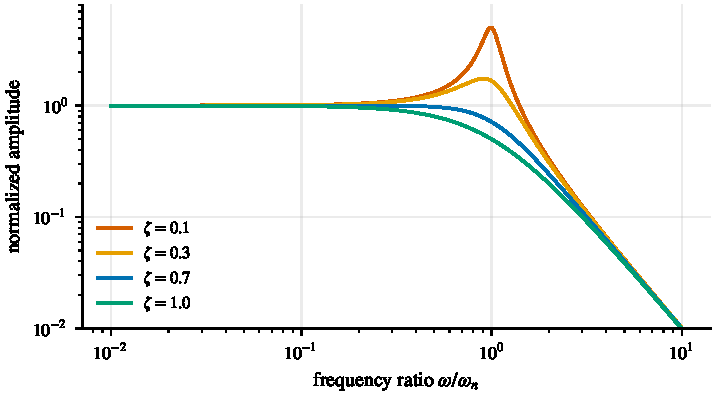
\includegraphics[width=0.84\textwidth]{fig_accel_bode.pdf}
  \caption{Frequency response of the spring-mass accelerometer model for several damping ratios. Below the natural frequency the response is flat: the
  deflection is proportional to specific force. A damping ratio near 0.7 gives the widest flat band without a resonant peak.}
  \label{fig:accel-bode}
\end{figure}

\subsection{Specific force}

\index{specific force}
The quantity measured is the \term{specific force}
\begin{equation}
  f = a - g,
\end{equation}
the non-gravitational force per unit mass acting on the sensor (the spring force divided by $m$). Gravity acts on the mass and the case equally
and cannot be felt directly: this is Einstein's equivalence principle. Two cases build intuition.
\begin{itemize}
  \item \textbf{At rest on a table}, $a = 0$, so $f = -g$. With $g_w = [0, 0, -9.81]\T$, the accelerometer reads $+9.81~\mathrm{m/s^2}$ \emph{upward}: it senses the table
        pushing it up.
  \item \textbf{In free fall}, $a = g$, so $f = 0$. A falling IMU reads zero, whatever its velocity.
\end{itemize}
To recover the kinematic acceleration from the measurement, the estimator rotates the specific force into the world frame and \emph{adds gravity back}:
$a_w = R_{wb}f_b + g_w$. A sign error here produces a vertical acceleration error of $2g \approx 20~\mathrm{m/s^2}$ and an obviously diverging altitude, which is
fortunately easy to recognize.

\paragraph{Noise.} Even a perfect mechanical sensor is noisy: the proof mass is jostled by the thermal motion of the surrounding gas, a
\emph{thermo-mechanical} noise whose acceleration density is about $\sqrt{4k_BT\omega_n/(mQ)}$ (with $k_B$ Boltzmann's constant, $T$ the temperature and $Q$ the
mechanical quality factor). Tiny masses are noisier, which is the basic trade-off of MEMS inertial sensing. Readout electronics add their own noise.

% ==============================================================================
\section{How a MEMS gyroscope works}

A MEMS \term{gyroscope} has no spinning wheel. It keeps a proof mass vibrating and detects the Coriolis force that rotation induces. Let the mass be
driven along the $x$-axis of the sensor at frequency $\omega_d$, so its velocity relative to the sensor is $v = A\omega_d\cos(\omega_dt)\,e_x$. If the sensor
rotates with angular velocity $\Omega$, then in the sensor frame the mass experiences the Coriolis acceleration $-2\Omega\times v$ (\cref{eq:coriolis}).
For a rotation about the $z$-axis this acceleration points along $y$:
\begin{equation}
  a_y = -2\,\Omega_z\,A\omega_d\cos(\omega_dt) .
\end{equation}
The resulting vibration along $y$ (the \emph{sense} mode) has an amplitude proportional to the rate $\Omega_z$ and oscillates at the drive frequency, so
the electronics recover $\Omega_z$ by demodulating the sense signal synchronously with the drive. The sensitive axis is perpendicular to both the drive and
the sense directions.

Real designs use two or four masses vibrating in anti-phase (a \emph{tuning fork}): their Coriolis forces are opposite and add in the differential
readout, while linear accelerations and vibrations push all masses the same way and cancel. Imperfect cancellation leaves a small sensitivity of the
gyro output to acceleration ($g$-sensitivity). Manufacturing asymmetries couple the drive into the sense mode (\emph{quadrature}), and their drift with
temperature is a major source of gyro bias.

% ==============================================================================
\section{The measurement model}

\subsection{The project's model}

\begin{convention}[IMU model, AGENTS.md C6]
\begin{equation}
  \omega_m = \omega_b + b_g + n_g, \qquad
  a_m = R_{wb}\T\big(a_w - g_w\big) + b_a + n_a, \qquad
  \dot b_g = n_{b_g}, \quad \dot b_a = n_{b_a},
  \label{eq:imu-model}
\end{equation}
with $\omega_m$, $a_m$ the gyroscope and accelerometer readings in the body frame, $\omega_b$ the true angular rate, $a_w$ the true acceleration of the body in the
world frame, $b_g$, $b_a$ the biases (body frame), and $n_g, n_a, n_{b_g}, n_{b_a}$ zero-mean white noises with densities $\sigma_g, \sigma_a, \sigma_{b_g}, \sigma_{b_a}$. The
noise vector is ordered $w = [n_a, n_g, n_{b_a}, n_{b_g}] \in \R^{12}$.
\end{convention}

The model has two kinds of error. \emph{White noise} ($n_g$, $n_a$) is independent from sample to sample and averages out. \emph{Bias} ($b_g$, $b_a$) is a slowly
varying offset that does not average out and is therefore estimated as part of the state (a shaping filter, \cref{ch:processes}). Its slow drift is
modeled as a random walk driven by $n_{b_g}$, $n_{b_a}$. Over the minutes of a EuRoC sequence the biases change little but measurably.

\subsection{A fuller error model}

High-accuracy inertial systems use a richer model, of which \eqref{eq:imu-model} is the special case $S = M = G = 0$:
\begin{equation}
  a_m = (I + S_a)M_a\,f_b + b_a + n_a, \qquad \omega_m = (I + S_g)M_g\,\omega_b + G_g\,f_b + b_g + n_g .
\end{equation}
Here $S$ is a diagonal matrix of \emph{scale-factor} errors (the output is $(1 + s)$ times the input), $M$ a near-identity matrix describing \emph{axis
misalignment and non-orthogonality} (the three sensing axes are neither exactly perpendicular nor exactly aligned with the body frame), and $G_g$ the
$g$-sensitivity of the gyroscope. Each of these parameters can be calibrated, estimated online as additional states, or ignored, at the cost of
some unmodeled error.

\begin{table}[t]
\centering\small
\begin{tabularx}{\textwidth}{@{}l X l@{}}
\toprule
\textbf{Error} & \textbf{Description} & \textbf{In the model?} \\
\midrule
White noise & sample-to-sample electronic and thermo-mechanical noise (angle/velocity random walk) & yes, $n_g$, $n_a$ \\
Turn-on bias & constant offset that differs at each power-up & yes, initial $b$ and $P_0$ \\
In-run bias drift & slow wandering of the offset & yes, random walk \\
Bias instability & flicker ($1/f$) noise floor of the bias & approximated by the random walk \\
Scale factor & output $= (1 + s)\times$ input & no \\
Axis misalignment & sensing axes not exactly orthogonal / aligned with the case & no \\
$g$-sensitivity & gyro output depends on acceleration & no \\
Temperature effects & bias and scale factor change with temperature & no (absorbed by bias walk) \\
Quantization & finite resolution of the ADC & no (below white noise) \\
Saturation, vibration & clipping on impacts; aliasing of high-frequency vibration & no \\
Earth rotation & gyros sense $7.3\times10^{-5}$~rad/s & no (\cref{ch:rotations}) \\
\bottomrule
\end{tabularx}
\caption{IMU error sources and how the project's model treats them.}
\label{tab:imu-errors}
\end{table}

\Cref{tab:imu-errors} lists the main error sources. Unmodeled errors do not disappear: they appear as apparent extra noise or apparent bias drift. A filter
that ignores them must compensate with larger noise parameters than the white-noise floor alone would suggest, which is why tuning is needed even with a
well-calibrated sensor. The size of the effect is easy to estimate: a scale-factor error of $10^{-3}$ on a gyro turning at 1~rad/s is an apparent bias of
$10^{-3}$~rad/s, as large as a poor bias and much larger than the EuRoC gyro's noise.

% ==============================================================================
\section{Calibration}

\paragraph{Gyroscope bias.} At rest, the gyroscope should read zero (or the Earth rate). Averaging a few seconds of data gives the bias, with a standard
deviation of $\sigma_g/\sqrt T$ after $T$ seconds (\cref{ch:processes}): for EuRoC, $10^{-4}$~rad/s after 3~s.

\paragraph{Accelerometer bias and scale: the six-position test.} Place the IMU with each axis pointing straight up and then straight down. For an axis with
bias $b$ and scale factor $1 + s$, the two readings are $(1 + s)g + b$ and $-(1 + s)g + b$, so
\begin{equation}
  b = \frac{a_{\mathrm{up}} + a_{\mathrm{down}}}{2}, \qquad 1 + s = \frac{a_{\mathrm{up}} - a_{\mathrm{down}}}{2g} .
\end{equation}
Using more orientations and a least-squares fit (\cref{ch:estimation}) also yields the misalignments.

\paragraph{Gyroscope scale and misalignment.} These require known rotations, from a rate table, or from a known sequence of orientations measured by an
accelerometer.

\paragraph{Camera--IMU calibration.} The extrinsic transform $T_{bc}$, the time offset between the sensors, and optionally the IMU's own scale and misalignment
are estimated jointly by moving the rig in front of a calibration target. The Kalibr toolbox~\cite{furgale2013kalibr}, which produced EuRoC's calibration,
represents the trajectory as a continuous-time B-spline and solves one large nonlinear least-squares problem (\cref{ch:nlls}) combining camera
reprojection errors and IMU residuals.

\paragraph{Temperature.} Biases and scale factors depend on temperature. Industrial IMUs are calibrated at several temperatures and compensated with an
on-board temperature sensor; consumer IMUs often are not, and a filter must track the resulting drift as bias random walk.

% ==============================================================================
\section{Noise parameters and their units}

The noise densities are continuous-time quantities (\cref{sec:ct-noise}). For EuRoC's ADIS16448, the \code{imu0/sensor.yaml} file gives the values in
\cref{tab:euroc-imu}.

\begin{table}[h]
\centering\small
\begin{tabular}{@{}l l l l@{}}
\toprule
YAML key & Symbol & Value & Units \\
\midrule
\code{gyroscope\_noise\_density} & $\sigma_g$ & $1.6968\times10^{-4}$ & $\mathrm{rad/s/\sqrt{Hz}}$ \\
\code{accelerometer\_noise\_density} & $\sigma_a$ & $2.0\times10^{-3}$ & $\mathrm{m/s^2/\sqrt{Hz}}$ \\
\code{gyroscope\_random\_walk} & $\sigma_{b_g}$ & $1.9393\times10^{-5}$ & $\mathrm{rad/s^2/\sqrt{Hz}}$ \\
\code{accelerometer\_random\_walk} & $\sigma_{b_a}$ & $3.0\times10^{-3}$ & $\mathrm{m/s^3/\sqrt{Hz}}$ \\
\code{rate\_hz} & $1/\Dt$ & 200 & Hz \\
\bottomrule
\end{tabular}
\caption{EuRoC IMU noise parameters (\code{imu0/sensor.yaml}). Verify against your copy of the dataset.}
\label{tab:euroc-imu}
\end{table}

The units follow from the definitions. A gyro rate in rad/s with a white noise density has units $\mathrm{rad/s}\cdot\sqrt{\mathrm{s}} = \mathrm{rad/s/\sqrt{Hz}}$. A gyro
bias random walk is the integral of white noise with units of $\mathrm{rad/s^2}$, so its density is in $\mathrm{rad/s^2/\sqrt{Hz}}$, and after $t$ seconds the
bias has standard deviation $\sigma_{b_g}\sqrt t$ in rad/s.

\paragraph{Discrete equivalents.} At sample period $\Dt$ (\cref{eq:discrete-noise}):
\begin{equation}
  \sigma_{g,d} = \frac{\sigma_g}{\sqrt\Dt}, \qquad \sigma_{a,d} = \frac{\sigma_a}{\sqrt\Dt}, \qquad
  \sigma_{b_g,d} = \sigma_{b_g}\sqrt\Dt, \qquad \sigma_{b_a,d} = \sigma_{b_a}\sqrt\Dt .
\end{equation}
For EuRoC: $\sigma_{g,d} = 2.4\times10^{-3}$~rad/s per sample, $\sigma_{a,d} = 2.8\times10^{-2}~\mathrm{m/s^2}$ per sample, and the gyro bias diffuses by
$1.4\times10^{-6}$~rad/s per sample. In the filter you never need these directly, because $Q_d = G_cQ_cG_c\T\Dt$ uses the densities, but they are what a synthetic
data generator must add to each sample.

\paragraph{Datasheet units.} Manufacturers often quote angle random walk (ARW) in $^\circ/\sqrt{\mathrm{h}}$ and velocity random walk (VRW) in $\mathrm{m/s/\sqrt{h}}$.
Since $1\ ^\circ/\sqrt{\mathrm{h}} = \frac{\pi/180}{60}~\mathrm{rad/\sqrt{s}} = 2.909\times10^{-4}~\mathrm{rad/s/\sqrt{Hz}}$, EuRoC's $\sigma_g$ is an ARW of $0.58\ ^\circ/\sqrt{\mathrm{h}}$,
and its $\sigma_a$ is a VRW of $0.12~\mathrm{m/s/\sqrt{h}}$. Bias instability is quoted in $^\circ/\mathrm{h}$ and is \emph{not} the same thing as the random walk
density.

\paragraph{Measuring them.} The densities are measured from a long static recording with the Allan variance (\cref{sec:allan,fig:allan}): white noise is read
off the slope $-\tfrac12$ at $\tau = 1$~s, and the bias random walk off the slope $+\tfrac12$ at $\tau = 3$~s.

% ==============================================================================
\section{Tuning in practice}

The densities from an Allan analysis describe a stationary sensor in a quiet lab. On a flying vehicle, vibration, temperature changes, scale-factor and
misalignment errors, timing jitter and integration error all add to the effective noise. Common practice is to start from the Allan values (or the
dataset's values) and inflate them by a modest factor until the filter is consistent, as judged by the statistical tests of \cref{ch:consistency}. Two
rules keep tuning honest.
\begin{enumerate}
  \item \textbf{Change physically meaningful parameters only}, and keep them within a plausible range of their measured values.
  \item \textbf{Judge on consistency statistics} (NEES on synthetic data, NIS and $3\sigma$ coverage on real data), not on trajectory error alone. Tuning for
        the lowest trajectory error on the test sequence is overfitting.
\end{enumerate}

\begin{pitfall}[mixing up the two discretizations]
The white-noise variance per sample is $\sigma^2/\Dt$ (larger at higher rate), while the random-walk variance per step is $\sigma_b^2\Dt$ (smaller at higher rate).
Swapping them is a common bug in synthetic data generators, and it produces noise that is wrong by a factor of $1/\Dt^2 = 40\,000$ at 200~Hz.
\end{pitfall}

\section{The EuRoC IMU stream}

EuRoC's \code{imu0/data.csv} contains one row per sample: \code{timestamp [ns], w\_x, w\_y, w\_z [rad/s], a\_x, a\_y, a\_z [m/s\textsuperscript{2}]}, i.e.\ $\omega_m$
and $a_m$ in $B$ (AGENTS.md C7). Samples arrive at nominally 200~Hz, hardware-synchronized with the cameras. The filter must nevertheless take $\Dt$ from
consecutive timestamps (AGENTS.md C5): real data has jitter and occasional gaps, which Milestone 3 logs. The ground-truth file starts later than the IMU
file, so the filter is initialized at the first ground-truth sample at or after the stream start.

\begin{projectlink}[Milestones 3 and 4]
M3 parses \code{sensor.yaml} into exactly the parameters of \cref{tab:euroc-imu} and builds the event stream. M4's synthetic trajectory generator produces
noise-free IMU data from \eqref{eq:imu-model}; adding noise with the discrete equivalents above turns it into the Monte Carlo generator of M5.
\end{projectlink}

\begin{takeaways}
\begin{itemize}
  \item An accelerometer is a spring-mass system whose deflection, below resonance, is proportional to specific force $f = a - g$: it reads $+g$ upward at rest
        and zero in free fall.
  \item A MEMS gyroscope measures the Coriolis force on a vibrating mass.
  \item $\omega_m = \omega_b + b_g + n_g$ and $a_m = R_{wb}\T(a_w - g_w) + b_a + n_a$, with random-walk biases; scale factors and misalignments are neglected.
  \item Biases and scale factors can be calibrated with static multi-position tests; camera--IMU extrinsics with a target and a continuous-time solver.
  \item Noise densities have units of $[u]/\sqrt{\mathrm{Hz}}$; per-sample white noise is $\sigma/\sqrt\Dt$, per-step bias diffusion is $\sigma_b\sqrt\Dt$.
  \item Unmodeled errors force noise inflation; tune on consistency, not on accuracy.
\end{itemize}
\end{takeaways}

\begin{exercises}
  \item An IMU lies on a table tilted by $10^\circ$ about its $x$-axis. Compute the ideal accelerometer reading. Which component reveals the tilt, and with what sign?
  \item A MEMS accelerometer has a resonance at 5~kHz. How large is its static deflection per $\mathrm{m/s^2}$? Compare with the size of a silicon atom
        ($\approx 0.2$~nm) and comment.
  \item Derive the gyroscope's Coriolis acceleration from \eqref{eq:coriolis}, and explain why a tuning-fork design rejects linear acceleration.
  \item A six-position test gives $a_{\mathrm{up}} = 9.83$ and $a_{\mathrm{down}} = -9.79~\mathrm{m/s^2}$ on one axis. Compute the bias and scale factor.
  \item A gyroscope datasheet gives ARW $= 0.2\ ^\circ/\sqrt{\mathrm{h}}$. Convert it to $\mathrm{rad/s/\sqrt{Hz}}$ and to the per-sample standard deviation at 400~Hz.
  \item A scale-factor error of $s = 10^{-3}$ affects a gyro on a vehicle spinning at 1~rad/s. What equivalent bias does it produce? Why can't a constant-bias model
        absorb it during maneuvers?
\end{exercises}

\chapter{Strapdown Propagation of the Nominal State}
\label{ch:strapdown}
\chaptermark{Strapdown Propagation} % short running header

\begin{objectives}
\begin{itemize}
  \item State the continuous-time nominal kinematics and understand each term.
  \item Derive the exact solution of the kinematics for constant inputs over a step.
  \item Compare Euler, midpoint and Runge--Kutta integration, and predict their convergence orders.
  \item Propagate to arbitrary timestamps, handle gaps, and initialize the nominal state.
  \item Understand IMU preintegration as used by optimization-based estimators.
\end{itemize}
\end{objectives}

A \emph{strapdown} inertial system has its sensors rigidly attached (strapped down) to the vehicle, as
opposed to mounted on a stabilized gimbal platform. All the work of keeping track of orientation is done in
software, by integrating the gyroscope. This chapter is about that integration.

% ------------------------------------------------------------------------------
\section{Continuous-time kinematics}

\subsection{The navigation equations}

\index{strapdown mechanization}
The \emph{mechanization equations} follow from three facts established earlier. The position changes with the velocity, $\dot p_{wb} = v_{wb}$. The
velocity changes with the acceleration, which by the definition of specific force (\cref{ch:imu}) is the measured specific force rotated into the world
frame plus gravity, $\dot v_{wb} = a_w = R_{wb}f_b + g_w$. And the attitude changes with the body angular velocity, $\dot R_{wb} = R_{wb}\sx{\omega_b}$
(\cref{sec:rot-kinematics}). Here the world frame is treated as inertial, with the effects of the Earth's rotation neglected or absorbed into gravity
and the gyro bias; \cref{ch:rotations} showed that they are tiny over the scales of a EuRoC flight. Substituting the IMU model,
$f_b = a_m - b_a - n_a$ and $\omega_b = \omega_m - b_g - n_g$, gives the true kinematics of \cref{ch:errordyn}, and replacing the unknown biases by their estimates and
setting the noise to zero gives the nominal kinematics.

\begin{convention}[nominal propagation, AGENTS.md F1]
\begin{equation}
  \hat a = a_m - \hat b_a,\quad \hat\omega = \omega_m - \hat b_g;\qquad
  \dot{\hat p} = \hat v,\quad \dot{\hat v} = \hat R_{wb}\,\hat a + g_w,\quad
  \dot{\hat q} = \tfrac12\,\hat q\qprod[0,\ \hat\omega],\quad \dot{\hat b}_a = \dot{\hat b}_g = 0 .
  \label{eq:nominal-ct}
\end{equation}
The attitude update is always multiplicative, $\hat q \gets \hat q\qprod\Exp_q(\hat\omega\Dt)$, followed by
normalization. The integration scheme for $p$ and $v$ is chosen and justified in Milestone 4 and logged
in \texttt{PROGRESS.md}.
\end{convention}

The equations form a cascade: attitude depends on the gyroscope only; velocity depends on attitude and the
accelerometer; position depends on velocity. Errors cascade the same way, which is the origin of the
$t^2$ and $t^3$ growth laws of \cref{ch:intro}.

% ------------------------------------------------------------------------------
\section{Exact solution for constant inputs}

Suppose $\hat\omega$ and $\hat a$ are constant over $[t_k, t_k + \Dt]$, which is what a zero-order hold of one
IMU sample assumes. Then the kinematics can be solved in closed form.

\begin{proposition}[Constant-input propagation]
\label{prop:exact-prop}
With $\hat\omega$, $\hat a$ constant over the step and $\phi = \hat\omega\Dt$,
\begin{align}
  \hat R_{k+1} &= \hat R_k\,\Exp(\phi), \\
  \hat v_{k+1} &= \hat v_k + g_w\Dt + \hat R_k\,\Dt\,\Jl(\phi)\,\hat a, \\
  \hat p_{k+1} &= \hat p_k + \hat v_k\Dt + \tfrac12 g_w\Dt^2 + \hat R_k\,\Dt^2\,N(\phi)\,\hat a,
\end{align}
where $N(\phi) = \sum_{j\ge0}\sx{\phi}^j/(j+2)! = \tfrac12 I + \frac{\theta - \sin\theta}{\theta^3}\sx{\phi} +
\frac{\theta^2/2 + \cos\theta - 1}{\theta^4}\sx{\phi}^2$ and $\theta = \|\phi\|$.
\end{proposition}
\begin{proof}
The attitude is \cref{prop:const-rate}. During the step $\hat R(t_k + s) = \hat R_k\Exp(\hat\omega s)$, so
$\hat v_{k+1} - \hat v_k = g_w\Dt + \hat R_k\int_0^\Dt\Exp(\hat\omega s)\,\dd s\,\hat a$, and
$\int_0^\Dt\Exp(\hat\omega s)\,\dd s = \Dt\int_0^1\Exp(u\phi)\,\dd u = \Dt\,\Jl(\phi)$ by \cref{thm:jr}. Integrating once more
gives the position, with $\int_0^\Dt\!\int_0^s\Exp(\hat\omega u)\,\dd u\,\dd s = \Dt^2N(\phi)$ by term-wise integration of
the exponential series, and the closed form follows from $\sx{\phi}^3 = -\theta^2\sx{\phi}$.
\end{proof}

For small $\phi$, $\Jl(\phi) \approx I + \tfrac12\sx{\phi}$ and $N(\phi) \approx \tfrac12 I + \tfrac16\sx{\phi}$. The
correction terms account for the rotation of the specific-force vector during the step. At 200~Hz and
1~rad/s, $\|\phi\| = 0.005$, so they change the velocity increment by about 0.25\%: small, but systematic.

% ------------------------------------------------------------------------------
\section{Numerical integration schemes}

Real inputs are not constant over a step: the IMU provides samples at $t_k$ and $t_{k+1}$, and the true signal
varies between them. Three families of schemes are common. All of them update the attitude
multiplicatively.

\paragraph{Euler with zero-order hold.} Use the sample at the start of the step for the whole step:
\begin{equation}
  \hat R_{k+1} = \hat R_k\Exp(\hat\omega_k\Dt), \quad
  \hat v_{k+1} = \hat v_k + (\hat R_k\hat a_k + g_w)\Dt, \quad
  \hat p_{k+1} = \hat p_k + \hat v_k\Dt + \tfrac12(\hat R_k\hat a_k + g_w)\Dt^2 .
\end{equation}
Local error $O(\Dt^2)$, global error $O(\Dt)$. The dominant error is essentially a \emph{half-sample time
shift}: using the sample from the start of the interval for the whole interval delays the signal by
$\Dt/2$ on average. To see the local error, expand the true velocity increment $\int_{t_k}^{t_{k+1}}a_w(t)\,\dd t = a_w(t_k)\Dt + \tfrac12\dot a_w(t_k)\Dt^2 + O(\Dt^3)$; Euler keeps
only the first term, so each step errs by $\tfrac12\dot a_w\Dt^2$, and the errors of the $T/\Dt$ steps accumulate to $O(\Dt)$.

\paragraph{Midpoint (trapezoidal).} Use the average of the two bounding samples:
\begin{equation}
  \hat R_{k+1} = \hat R_k\Exp\big(\tfrac12(\hat\omega_k + \hat\omega_{k+1})\Dt\big),\quad
  \bar a_w = \tfrac12\big(\hat R_k\hat a_k + \hat R_{k+1}\hat a_{k+1}\big) + g_w,
\end{equation}
\begin{equation*}
  \hat v_{k+1} = \hat v_k + \bar a_w\Dt, \qquad \hat p_{k+1} = \hat p_k + \hat v_k\Dt + \tfrac12\bar a_w\Dt^2 .
\end{equation*}
Local error $O(\Dt^3)$, global $O(\Dt^2)$, at the cost of having to wait for the next sample before
completing the step.

\paragraph{Runge--Kutta 4.} RK4 evaluates the dynamics at the start, twice at the middle, and at the end of
the step. Its global error is $O(\Dt^4)$ \emph{if} the inputs at mid-step are known exactly. With an IMU
they are not, and must be interpolated from the bounding samples. Linear interpolation is only
second-order accurate, which caps the whole scheme at $O(\Dt^2)$.

\begin{figure}[t]
  \centering
  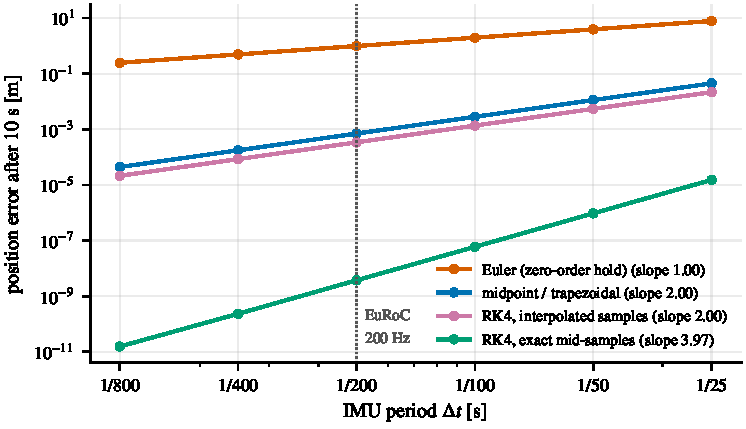
\includegraphics[width=0.86\textwidth]{fig_integration_order.pdf}
  \caption{Position error after 10~s of noise-free integration on a synthetic trajectory (2~m circle at
  0.8~rad/s with $\pm23^\circ$ roll oscillations), as a function of the IMU period. The measured slopes
  match the predicted global orders. RK4 reaches fourth order only with exact mid-step inputs, which a
  real IMU does not provide; with interpolated inputs it is no better than the midpoint rule.}
  \label{fig:integration-order}
\end{figure}

\Cref{fig:integration-order} confirms the predicted orders. Halving $\Dt$ divides the error by 2 for Euler and
by 4 for the midpoint rule, which is exactly the convergence-order test of Milestone 4. The magnitudes
matter as much as the slopes. At 200~Hz on this fairly dynamic trajectory, the Euler scheme accumulates
about a meter of error in 10~s, far more than the sensor noise would cause (\cref{fig:cov-growth}), because the
half-sample delay of the attitude creates a tilt error of order $\tfrac12\omega\Dt$, which leaks gravity. The
midpoint rule is three orders of magnitude better. On gentler motion the difference shrinks, and frequent
visual updates bound integration error in any case, but the integration error should be well below the
noise-induced error, or it becomes an unmodeled error that the filter cannot account for.

\begin{keyidea}[choosing a scheme]
The integration error is a deterministic, unmodeled error. The scheme should make it small compared with
the stochastic error the filter does model. Whichever scheme Milestone 4 adopts, document its order and
verify it with the halving test on a trajectory with closed-form ground truth.
\end{keyidea}

% ------------------------------------------------------------------------------
\section{Coning, sculling and the rotation-vector equation}
\label{sec:coning}

\subsection{The rotation vector of a step}

The attitude update over a step is a rotation $\Delta R = R(t_k)\T R(t_{k+1})$, which we can write as $\Exp(\phi)$ for a rotation vector $\phi$. If the angular
velocity keeps a fixed direction during the step, $\phi = \int\omega\,\dd t$. If its direction changes, this is wrong (\cref{prop:stm}), and the correct $\phi$
obeys a differential equation of its own.

\begin{proposition}[Bortz equation]
\label{prop:bortz}
\index{Bortz equation}
The rotation vector $\phi(t)$ with $\Exp(\phi(t)) = R(t_k)\T R(t)$ satisfies
\begin{equation}
  \dot\phi = \Jrinv(\phi)\,\omega = \omega + \tfrac12\,\phi\times\omega + D(\|\phi\|)\,\phi\times(\phi\times\omega),
\end{equation}
with $D$ the coefficient function of \cref{thm:jr}.
\end{proposition}
\begin{proof}
Over an instant $\dd t$, $\Exp(\phi + \dot\phi\,\dd t) = \Exp(\phi)\Exp(\omega\,\dd t)$. By the definition of the right Jacobian \eqref{eq:jr-def}, the left side is
$\Exp(\phi)\Exp(\Jr(\phi)\dot\phi\,\dd t)$, so $\Jr(\phi)\dot\phi = \omega$. Expand $\Jrinv$ with \eqref{eq:jrinv}.
\end{proof}

The term $\tfrac12\phi\times\omega$ is non-zero only when $\omega$ is not parallel to the rotation already accumulated: it is the \emph{non-commutativity
correction}. Under \emph{coning motion}, in which the angular velocity vector itself rotates (for example $\omega = (a\cos\Omega t,\ a\sin\Omega t,\ 0)$, the motion of
a vibrating or wobbling body), this correction does not average to zero. Integrating the rate vector alone then produces a steady, spurious
rotation about the cone axis, a drift that no amount of averaging removes.

\subsection{The two-sample coning correction}

Given the integrated gyro increments $\alpha_1$ and $\alpha_2$ over the two halves of a step (which a high-rate IMU, or two consecutive samples, provides),
the rotation vector of the whole step is, to third order,
\begin{equation}
  \phi \approx \alpha_1 + \alpha_2 + \tfrac23\,\alpha_1\times\alpha_2 .
  \label{eq:coning}
\end{equation}
\begin{proof}[Derivation]
Keep the first-order Bortz equation $\dot\phi \approx \omega + \tfrac12\phi\times\omega$ and suppose the rate varies linearly over the step, $\omega(s) = a + bs$ for
$s \in [0, h]$. To the needed order $\phi(s) \approx \int_0^s\omega = as + \tfrac12bs^2$, so
\begin{align*}
  \phi(h) &\approx \int_0^h\omega\,\dd s + \frac12\int_0^h\big(as + \tfrac12bs^2\big)\times(a + bs)\,\dd s \\
       &= \int_0^h\omega\,\dd s + \frac12(a\times b)\int_0^h\big(s^2 - \tfrac12s^2\big)\dd s
       = \alpha_1 + \alpha_2 + \frac{h^3}{12}\,a\times b .
\end{align*}
The half-step increments are $\alpha_1 = \tfrac h2a + \tfrac{h^2}8b$ and $\alpha_2 = \tfrac h2a + \tfrac{3h^2}8b$, whose cross product is $\alpha_1\times\alpha_2 = \tfrac{h^3}8\,a\times b$.
Hence $\tfrac{h^3}{12}a\times b = \tfrac23\alpha_1\times\alpha_2$.
\end{proof}

\begin{figure}[t]
  \centering
  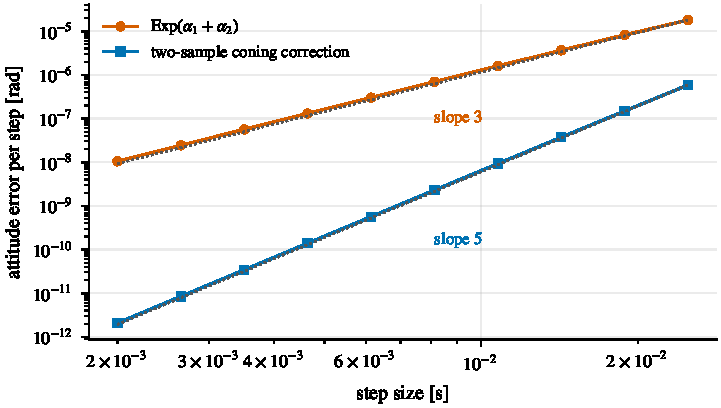
\includegraphics[width=0.84\textwidth]{fig_coning.pdf}
  \caption{Attitude error over one step under coning motion (rate amplitude 0.5~rad/s, coning frequency 10~Hz), as a function of the step size.
  Exponentiating the integrated rate errs at third order; the two-sample correction \eqref{eq:coning} reduces the error to fifth order.}
  \label{fig:coning}
\end{figure}

\Cref{fig:coning} confirms the orders. \emph{Sculling} is the analogous effect for velocity: when rotation and acceleration oscillate in phase, the
specific force is rotated while it is being integrated, and the error rectifies into a velocity drift; it has similar multi-sample corrections. High-end
inertial systems, with gyros sampled at kHz rates on vibrating platforms, rely on such algorithms~\cite{groves2013principles}. For a MEMS IMU sampled at
200~Hz, with vibration filtered by the sensor's own electronics, the effects are small compared with the sensor noise, and the project's single-sample
schemes suffice. The analysis still matters: it tells you what you are neglecting, and how to check that it is negligible.

% ------------------------------------------------------------------------------
\section{Timing}

\subsection{Propagating to an arbitrary time}

Images arrive between IMU samples. To clone the state at an image time $t_c \in (t_k, t_{k+1})$ (AGENTS.md F5), the
filter must propagate exactly to $t_c$: interpolate the IMU reading at $t_c$ linearly between samples $k$ and
$k+1$, propagate from $t_k$ to $t_c$ with the interpolated input, clone, and then propagate from $t_c$ to $t_{k+1}$.
The covariance follows the same split, with $\Dt$ replaced by the two partial intervals.

\subsection{Event ordering and gaps}

Measurements must be processed in timestamp order, and the state must be propagated to a measurement's time
before the measurement is applied (\cref{ch:fullalgo}). Milestone 3 fixes the tie rule: an IMU sample precedes a
measurement with an equal timestamp, so the state is propagated to that time first. Gaps in the IMU stream
(intervals larger than about $1.5$ nominal periods) must not be assumed away. $\Dt$ always comes from the
timestamps, and a long gap simply produces a long step with a correspondingly large $Q_d$.

% ------------------------------------------------------------------------------
\section{Initialization}

\subsection{From ground truth}

The project initializes the nominal state from the first ground-truth sample at or after the start of the
stream (Milestone 4): $p$, $v$, $q$, $b_a$ and $b_g$ all come from the ground-truth columns, mapped with the
column order of AGENTS.md C7. This isolates propagation from the initialization problem. The use of ground
truth for initialization is logged when the full VIO runs (Milestone 10b).

\subsection{Static initialization}

A real system initializes from its own sensors. If the vehicle is at rest for about a second,
\begin{equation}
  \bar a_m = \mathrm{mean}(a_m) \approx R_{wb}\T(-g_w) + b_a, \qquad \bar\omega_m = \mathrm{mean}(\omega_m) \approx b_g .
\end{equation}
The gyro bias is the mean rate. Neglecting $b_a$, the unit vector $u_b = \bar a_m/\|\bar a_m\|$ is the world
``up'' direction expressed in the body frame, $u_b = R_{wb}\T e_z$. Any rotation with $R_{wb}u_b = e_z$ is consistent
with it. One such rotation turns $u_b$ onto $e_z$ about the axis perpendicular to both:
\begin{equation}
  R_{wb} = \Exp\!\Big(\atantwo\big(\|u_b\times e_z\|,\ u_b\T e_z\big)\,\frac{u_b\times e_z}{\|u_b\times e_z\|}\Big),
\end{equation}
(with $R_{wb} = I$ if $u_b = e_z$ already), and composing it on the left with any rotation $R_z(\psi)$ about the vertical gives all the others. Roll and pitch are
determined; yaw is arbitrary, and is set to zero (or to the ground-truth yaw for evaluation).

\begin{pitfall}[tilt and accelerometer bias are indistinguishable at rest]
A horizontal accelerometer bias $b_a$ produces the same reading as a tilt of $\|b_a\|/g$: a bias of
$10~\mathrm{mm/s^2}$ looks exactly like a tilt of $1$~mrad. At rest the filter cannot separate them, and the initial
covariance must say so (large $\sigma_{b_a}$, correlated with the tilt). They become separable once the vehicle
rotates, because the bias rotates with the body while gravity does not.
\end{pitfall}

Initial covariances should reflect real uncertainty: a few milliradians in roll and pitch, a large or
unknown yaw, the turn-on bias range from the datasheet, and a small but non-zero velocity uncertainty at rest.
\emph{Dynamic} initialization from a moving start, as in VINS-Mono~\cite{qin2018vins}, first solves a
vision-only structure-from-motion problem and then aligns it with preintegrated IMU data to recover scale,
gravity and velocity.

% ------------------------------------------------------------------------------
\section{Sidebar: IMU preintegration}

An optimization-based estimator may relinearize a window of states many times. Re-integrating every IMU
sample between keyframes $i$ and $j$ each time the estimate of state $i$ changes would be wasteful.
\emph{Preintegration}~\cite{lupton2012visual, forster2017preintegration} integrates the measurements in the body frame
of keyframe $i$, so that the result does not depend on the state at $i$:
\begin{equation}
  \Delta R_{ij} = \prod_{k=i}^{j-1}\Exp(\hat\omega_k\Dt), \quad
  \Delta v_{ij} = \sum_{k=i}^{j-1}\Delta R_{ik}\,\hat a_k\Dt, \quad
  \Delta p_{ij} = \sum_{k=i}^{j-1}\Big(\Delta v_{ik}\Dt + \tfrac12\Delta R_{ik}\,\hat a_k\Dt^2\Big).
\end{equation}
These relate the two keyframe states through
$R_j = R_i\Delta R_{ij}$, $v_j = v_i + g\Delta t_{ij} + R_i\Delta v_{ij}$ and
$p_j = p_i + v_i\Delta t_{ij} + \tfrac12g\Delta t_{ij}^2 + R_i\Delta p_{ij}$. The preintegrated quantities depend on the
bias estimate, and first-order bias Jacobians avoid re-integration when the bias estimate changes. A filter
like the MSCKF does not need preintegration, because it integrates each sample exactly once.

\begin{projectlink}[Milestone 4]
Exit criteria: a stationary input keeps the state constant to $10^{-9}$ for 60~s; a constant rate reproduces
$q_0\qprod\Exp_q(\omega t)$; a circular trajectory converges at the predicted order; the quaternion norm stays
within $10^{-12}$ of one after $10^6$ steps; propagation does not allocate; and 10~s of dead reckoning on
MH\_01 produce no NaN.
\end{projectlink}

\begin{takeaways}
\begin{itemize}
  \item $\dot p = v$, $\dot v = R\hat a + g$, $\dot q = \tfrac12 q\qprod[0,\hat\omega]$; attitude updates are multiplicative.
  \item For constant inputs the solution is exact: $R\Exp(\phi)$, $v + g\Dt + R\Dt\Jl(\phi)\hat a$, and a similar
        position formula.
  \item Euler is first order (a half-sample delay), midpoint second order. RK4 is limited to second order by
        input interpolation.
  \item Integration error is unmodeled error; keep it well below sensor-noise error and verify the order.
  \item Propagate exactly to measurement times by splitting the IMU interval.
  \item At rest, gravity gives roll and pitch, the mean gyro gives $b_g$, and tilt and horizontal $b_a$ are
        indistinguishable.
\end{itemize}
\end{takeaways}

\begin{exercises}
  \item Verify \cref{prop:exact-prop} numerically by comparing with an ODE solver at tight tolerance.
  \item Show that the Euler scheme applied to a constant rotation rate is exact for the attitude, but not for
        the velocity, and quantify the velocity error per step in terms of $\|\hat\omega\|\Dt$.
  \item Reproduce \cref{fig:integration-order}. Then add gyro noise and plot the noise-induced position error
        on the same axes. At what IMU rate does integration error fall below noise error for each scheme?
  \item Implement the static initializer and test it on synthetic data with a known tilt. Add a horizontal
        accelerometer bias and show that it biases the estimated tilt by $\|b_a\|/g$.
  \item Why must the propagation to an image timestamp interpolate the IMU sample instead of using the
        nearest sample? Estimate the attitude error from using the nearest sample at 1~rad/s and 200~Hz.
\end{exercises}
% Solutions to the exercises of Chapter 16.
\begin{solutions}
  \item Choose a non-trivial initial state ($R_0 = \Exp(0.2, -0.1, 0.4)$, $v_0 = (1, 0.5, -0.2)$, $p_0 = (0.1, 0.2, 0.3)$), constant inputs
        $\hat\omega = (0.3, -0.5, 0.8)$~rad/s and $\hat a = (1, -2, 9)~\mathrm{m/s^2}$, and a long step $\Dt = 0.5$~s so that $\|\phi\| = 0.5$~rad and the correction terms
        are large. Integrating $\dot R = R\sx{\hat\omega}$, $\dot v = R\hat a + g_w$, $\dot p = v$ with \code{scipy.integrate.solve\_ivp} (DOP853, tolerances $10^{-13}$) and
        comparing with \cref{prop:exact-prop} gives differences of $2\times10^{-15}$ in $R$ and $8\times10^{-15}$ in $v$ and $p$: the closed forms are exact. Setting
        $\Jl = I$ and $N = \tfrac12I$ instead produces errors of order $\tfrac12\|\phi\|\,\|\hat a\|\Dt$, many orders of magnitude larger.

  \item With constant $\hat\omega$ the Euler scheme's attitude update $\hat R_k\Exp(\hat\omega\Dt)$ is exactly \cref{prop:const-rate}. Its velocity update uses
        $\hat R_k\hat a\,\Dt$, while the exact increment is $\hat R_k\Dt\Jl(\phi)\hat a$ with $\Jl(\phi) = I + \tfrac12\sx{\phi} + O(\|\phi\|^2)$. The error per step is
        \[
          \hat R_k\Dt\big(\Jl(\phi) - I\big)\hat a = \tfrac12\hat R_k\,\Dt^2\,\hat\omega\times\hat a + O(\Dt^3),
        \]
        a fraction $\tfrac12\|\hat\omega\|\Dt\sin\angle(\hat\omega, \hat a)$ of the step's velocity increment: $0.25\%$ at 1~rad/s and 200~Hz (a numerical check gives
        exactly $0.0025$). It is the effect of holding the specific force fixed in the body frame at the start of the step while the body rotates;
        it is systematic, so it accumulates.

  \item Running the code of \cref{fig:integration-order} gives position errors after 10~s at 200~Hz of $1.0$~m (Euler), $7\times10^{-4}$~m (midpoint) and
        $3\times10^{-4}$~m (RK4 with interpolated mid-samples), each scaling with its order. Adding EuRoC's gyro and accelerometer white noise to the
        samples and repeating 40 times gives a noise-induced RMS position error of about $0.17$--$0.19$~m after 10~s, the same at 100, 200 and 800~Hz:
        sampling faster does not reduce the noise per unit time (\cref{sec:ct-noise}). The noise error is therefore a horizontal line on the plot, and
        each integration error curve crosses it where:
        \begin{itemize}[leftmargin=1.2em]
          \item Euler: its error $\approx 1.0~\mathrm m\times(200/f)$ falls below $0.18$~m only above about $1.1$~kHz, faster than most MEMS IMUs deliver;
          \item midpoint and interpolated RK4: their errors are below the noise at every rate tested, down to 25~Hz ($0.045$ and $0.022$~m).
        \end{itemize}
        At EuRoC's 200~Hz a second-order scheme makes the integration error two to three orders of magnitude smaller than the noise, which is the
        requirement of \cref{ch:strapdown}.

  \item Generate one second of static accelerometer samples at 200~Hz for a known tilt (roll $5^\circ$, pitch $-3^\circ$) with EuRoC noise, average them, and apply
        the initializer. The estimated ``up'' direction is within $0.2$~mrad of the truth (the residual is the noise of the average,
        $\sigma_a/\sqrt{1\,\mathrm s}/g$ per axis). Adding a body-frame bias $b_a = (0.05, 0, 0)~\mathrm{m/s^2}$, almost horizontal for this attitude, moves the estimate by
        $4.9$~mrad, against the prediction $\|b_{a,\perp}\|/g = 5.1$~mrad, where $b_{a,\perp}$ is the component perpendicular to gravity (the difference is the noise
        of the average). The reason: the initializer takes the direction of $R\T(-g_w) + b_a$ to be ``up''; a horizontal bias tilts that vector by
        $\arctan(\|b_{a,\perp}\|/g) \approx \|b_{a,\perp}\|/g$, and nothing in a static recording distinguishes it from a real tilt.

  \item The clone must be the pose at the image timestamp $t_c$. Propagating only to the nearest IMU sample makes the clone the pose at a time that
        differs from $t_c$ by up to half a sample period, $\Dt/2 = 2.5$~ms at 200~Hz (1.25~ms on average, for a uniformly distributed offset). At 1~rad/s
        the attitude error is up to $2.5$~mrad, comparable to the angle subtended by one pixel of the EuRoC camera ($1/458 \approx 2.2$~mrad), and at 1~m/s the
        position error is up to $2.5$~mm. Unlike pixel noise this error is not random from the filter's point of view: it is correlated with the motion,
        so it biases every visual constraint during fast rotations. Interpolating the IMU sample at $t_c$ and propagating exactly to it removes the error
        at no cost.
\end{solutions}


\chapter{Error-State Dynamics and Covariance Propagation}
\label{ch:errordyn}
\chaptermark{Error-State Dynamics} % short running header

\begin{objectives}
\begin{itemize}
  \item Set up the 15-dimensional IMU error state with the frozen index layout.
  \item Derive linearized error dynamics with the four-step recipe, including the attitude error under a
        perturbation convention.
  \item Discretize into $\Phi$ and $Q_d$ and propagate the covariance of the IMU state and its clones.
  \item Predict analytically how fast each noise source inflates the position uncertainty.
  \item Validate the propagation by finite differences and by Monte Carlo simulation.
\end{itemize}
\end{objectives}

% ------------------------------------------------------------------------------
\section{True and nominal systems}

The true state evolves under the IMU model \eqref{eq:imu-model} solved for the physical quantities. With
$\omega = \omega_m - b_g - n_g$ and $a = a_m - b_a - n_a$ the true body rate and specific force,
\begin{equation}
  \dot p = v, \qquad \dot v = R\,(a_m - b_a - n_a) + g_w, \qquad \dot R = R\,\sx{\omega_m - b_g - n_g},
  \qquad \dot b_a = n_{b_a}, \qquad \dot b_g = n_{b_g},
  \label{eq:true-ct}
\end{equation}
where $R = R_{wb}$. The nominal state follows \eqref{eq:nominal-ct}, which is \eqref{eq:true-ct} with the biases replaced
by their estimates and the noise set to zero. The error state measures their difference.

\begin{convention}[error-state layout, AGENTS.md C3]
\begin{center}\small
\begin{tabular}{@{}c c l@{}}
\toprule
Indices & Block & Meaning \\
\midrule
0--2 & $\delta p$ & position error, world frame \\
3--5 & $\delta v$ & velocity error, world frame \\
6--8 & $\delta\theta$ & attitude error, \textbf{body frame (local)}: $R = \hat R\Exp(\delta\theta)$ \\
9--11 & $\delta b_a$ & accelerometer bias error \\
12--14 & $\delta b_g$ & gyroscope bias error \\
$15+6i$ \dots $+2$ & $\delta p_i$ & clone $i$ position error \\
$18+6i$ \dots $+2$ & $\delta\theta_i$ & clone $i$ attitude error (local) \\
\bottomrule
\end{tabular}
\end{center}
Noise ordering: $w = [n_a, n_g, n_{b_a}, n_{b_g}] \in \R^{12}$.
\end{convention}

Index constants belong in one place in the code (\code{constexpr} offsets in \code{types.hpp}), and every block
access goes through them. Hard-coded literals such as \code{P.block<3,3>(6,6)} scattered through the code are how
layout bugs are born.

% ------------------------------------------------------------------------------
\section{Deriving the error dynamics}
\label{sec:deriving-Fc}

The goal is the linear system
\begin{equation}
  \dot{\delta x}_I = F_c\,\delta x_I + G_c\,w, \qquad F_c \in \R^{15\times15},\quad G_c \in \R^{15\times12},
\end{equation}
obtained with the recipe of \cref{sec:error-dyn-recipe}. Two of the five blocks are immediate.

\paragraph{Position.} Substituting $p = \hat p + \delta p$ and $v = \hat v + \delta v$ into $\dot p = v$ and subtracting
$\dot{\hat p} = \hat v$ gives $\dot{\delta p} = \delta v$ exactly. No linearization is needed.

\paragraph{Biases.} $\dot b_a = n_{b_a}$ and $\dot{\hat b}_a = 0$ give $\dot{\delta b}_a = n_{b_a}$, and likewise
$\dot{\delta b}_g = n_{b_g}$.

The velocity and attitude blocks involve the rotation and require the Lie tools of \cref{ch:lie}. One lemma
handles the time derivative of the perturbation itself.

\begin{lemma}[Time derivative of a perturbation]
\label{lem:dexp}
For a differentiable $\delta\theta(t)$,
$\frac{\dd}{\dd t}\Exp(\delta\theta) = \Exp(\delta\theta)\sx{\Jr(\delta\theta)\,\dot{\delta\theta}} = \sx{\Jl(\delta\theta)\,\dot{\delta\theta}}\Exp(\delta\theta)$.
To first order in $\delta\theta$, both reduce to $\sx{\dot{\delta\theta}}$ multiplying $\Exp(\delta\theta)$ on the corresponding side.
\end{lemma}
\begin{proof}
Apply the definition \eqref{eq:jr-def} of $\Jr$ and $\Jl$ with $\delta = \dot{\delta\theta}\,\dd t$.
\end{proof}

\subsection{Worked example: attitude error under the global perturbation}

To demonstrate the method without solving the project's exercise, we first derive the attitude error
dynamics for the \emph{global} perturbation $R = \Exp(\delta\theta_g)\hat R$. This is \textbf{not} the project's
convention; it is here for contrast.

\begin{example}[Global attitude error dynamics]
\label{ex:global-attitude}
Differentiate both sides of $R = \Exp(\delta\theta_g)\hat R$ using \cref{lem:dexp} to first order and the kinematics
$\dot R = R\sx{\omega}$, $\dot{\hat R} = \hat R\sx{\hat\omega}$:
\begin{equation*}
  \underbrace{\Exp(\delta\theta_g)\hat R\sx{\omega}}_{\dot R}
  \approx \sx{\dot{\delta\theta}_g}\Exp(\delta\theta_g)\hat R + \Exp(\delta\theta_g)\hat R\sx{\hat\omega}.
\end{equation*}
Move the last term to the left and use $\omega - \hat\omega = -\delta b_g - n_g$:
\begin{equation*}
  \sx{\dot{\delta\theta}_g}\Exp(\delta\theta_g)\hat R \approx \Exp(\delta\theta_g)\hat R\sx{-\delta b_g - n_g}.
\end{equation*}
Multiply on the right by $(\Exp(\delta\theta_g)\hat R)\T$ and apply \eqref{eq:skew-rot} with the rotation $\Exp(\delta\theta_g)\hat R$:
\begin{equation*}
  \sx{\dot{\delta\theta}_g} \approx \sx{\Exp(\delta\theta_g)\hat R(-\delta b_g - n_g)} \approx \sx{-\hat R\,\delta b_g - \hat R\, n_g},
\end{equation*}
where the last step drops the product of $\delta\theta_g$ with $\delta b_g$ and $n_g$, both small. Hence
\begin{equation}
  \dot{\delta\theta}_g = -\hat R\,\delta b_g - \hat R\,n_g .
\end{equation}
The global attitude error does not depend on itself at all: the world-frame error is constant unless driven by
gyro errors, which are rotated into the world by $\hat R$.
\end{example}

\subsection{Your turn: the local (right) perturbation}

\begin{derivex}{attitude and velocity rows of $F_c$ and $G_c$}{sol:Fc}
Derive $\dot{\delta\theta}$ and $\dot{\delta v}$ under the project's local perturbation $R = \hat R\Exp(\delta\theta)$.
\begin{enumerate}
  \item \textbf{Attitude.} Differentiate $R = \hat R\Exp(\delta\theta)$ with \cref{lem:dexp} (right form). Cancel the nominal
        term, then use $\Exp(-\delta\theta)\sx{\hat\omega}\Exp(\delta\theta) = \sx{\Exp(-\delta\theta)\hat\omega}$ and
        $\Exp(-\delta\theta)\hat\omega \approx \hat\omega - \delta\theta\times\hat\omega$. You should find a term proportional to $\delta\theta$ that the global
        version lacks. Explain it physically: what happens to a body-frame error when the body rotates?
  \item \textbf{Velocity.} Substitute $R = \hat R\Exp(\delta\theta) \approx \hat R(I + \sx{\delta\theta})$ and
        $a_m - b_a - n_a = \hat a - \delta b_a - n_a$ into $\dot v = R(a_m - b_a - n_a) + g_w$, subtract
        $\dot{\hat v} = \hat R\hat a + g_w$, drop second-order products, and use \eqref{eq:skew-anticomm} to move $\delta\theta$ to the
        right.
  \item \textbf{Assemble} $F_c$ and $G_c$ in the frozen order of AGENTS.md C3. Before filling any block, predict
        from the cascade structure of the kinematics which blocks must be zero.
\end{enumerate}
\textbf{Check:} build $\Phi \approx I + F_c\Dt$ and compare each column with
$\big(f(\hat x\bplus\epsilon e_i)\bminus f(\hat x)\big)/\epsilon$ for one step $f$ of your nominal integrator, at a state with
non-identity attitude, non-zero rates, specific force and biases (Milestone 5). Agreement must be at the level
of the $O(\Dt^2)$ terms neglected by $I + F_c\Dt$. Then record the result in \code{DOCS/derivations.md}.
\end{derivex}

Physically, the velocity row you will find encodes the most important coupling in inertial navigation: an
attitude error tilts the computed specific force, so a fraction of the large vector $\hat a$ (dominated by the
reaction to gravity, $9.81~\mathrm{m/s^2}$) leaks into the velocity error. That single term is behind the
$t^3$ law of \cref{ch:intro}.

% ------------------------------------------------------------------------------
\section{Discretization}

Over one IMU step the error dynamics are discretized as in \cref{sec:discretization} (AGENTS.md F2):
\begin{equation}
  \Phi \approx I_{15} + F_c\Dt, \qquad
  Q_c = \diag\big(\sigma_a^2 I_3,\ \sigma_g^2 I_3,\ \sigma_{b_a}^2 I_3,\ \sigma_{b_g}^2 I_3\big), \qquad
  Q_d \approx G_c Q_c G_c\T\Dt ,
  \label{eq:imu-discretization}
\end{equation}
with $F_c$ and $G_c$ evaluated at the nominal state and the bias-corrected IMU inputs at the beginning of the
step (or at the midpoint, consistently with the chosen integration scheme). The densities are the
continuous-time values of \cref{tab:euroc-imu}; the $\Dt$ in $Q_d$ converts them into variances
accumulated during the step.

\begin{remark}[higher-order options]
$F_c$ is block upper-triangular with a large nilpotent part, so $\exp(F_c\Dt)$ has a closed form. In particular the
attitude block of the exact $\Phi$ is a rotation matrix, while the first-order block is not exactly orthogonal. At
200~Hz and 1~rad/s the difference per step is about $(\|\hat\omega\|\Dt)^2/2 \approx 10^{-5}$, below the noise.
Adopting a higher-order $\Phi$ is allowed if it is logged (AGENTS.md F2). Van Loan's method
(\cref{prop:vanloan}) gives exact reference values for testing whichever form is used.
\ifsolutions The closed-form blocks are listed with the solutions in \cref{sol:Phi}.\fi
\end{remark}

\paragraph{The continuous-time view.} The discrete recursion is a numerical integration of a differential equation for the covariance.
For the linear stochastic system $\dot{\delta x} = F_c\,\delta x + G_c\,w$, the covariance obeys the Lyapunov differential equation of
\cref{prop:lyapunov},
\begin{equation}
  \dot P = F_cP + PF_c\T + G_cQ_cG_c\T .
  \label{eq:imu-lyapunov}
\end{equation}
Substituting $\Phi = I + F_c\Dt$ and $Q_d = G_cQ_cG_c\T\Dt$ into one step gives
$\Phi P\Phi\T + Q_d = P + \big(F_cP + PF_c\T + G_cQ_cG_c\T\big)\Dt + F_cPF_c\T\Dt^2$: the filter's propagation is Euler's method applied to
\eqref{eq:imu-lyapunov}, with a local error of $O(\Dt^2)$. Each term has a meaning. $G_cQ_cG_c\T$ injects uncertainty where the noise enters (velocity,
attitude and the biases), and $F_cP + PF_c\T$ transports it along the couplings of $F_c$: from biases into attitude and velocity, from attitude into
velocity, from velocity into position. The growth laws of \cref{prop:growth-laws} below are exact solutions of \eqref{eq:imu-lyapunov} for a level,
stationary IMU, and they are the reference against which the discrete propagation is tested in Milestone 5.

% ------------------------------------------------------------------------------
\section{Propagating the full covariance}

With $N$ clones the state has dimension $n = 15 + 6N$, and the covariance is partitioned as
\begin{equation}
  P = \begin{bmatrix} P_{II} & P_{IC} \\ P_{CI} & P_{CC} \end{bmatrix},
  \qquad P_{II}\in\R^{15\times15},\ P_{IC}\in\R^{15\times6N},\ P_{CC}\in\R^{6N\times6N}.
\end{equation}
Clones are frozen copies of past poses, so their error dynamics are zero: $\dot{\delta x}_C = 0$. The full
transition matrix is $\blkdiag(\Phi, I_{6N})$, and the full process noise is $\blkdiag(Q_d, 0)$. Multiplying out:

\begin{convention}[covariance propagation, AGENTS.md F2]
\begin{equation}
  P_{II} \gets \Phi P_{II}\Phi\T + Q_d, \qquad P_{IC} \gets \Phi P_{IC}, \qquad P_{CI} = P_{IC}\T, \qquad P_{CC}\ \text{unchanged},
\end{equation}
followed by $P \gets \tfrac12(P + P\T)$.
\end{convention}

The block form is not only a convenience. Updating only the affected blocks costs $\mathcal{O}(15^2\cdot 6N)$ per step
instead of $\mathcal{O}(n^3)$, and it never touches the large $P_{CC}$ block between images. The cross-covariance
$P_{IC}$ is what remembers that the clones and the current state share a history. It is what lets a visual
constraint between two past poses correct the current velocity and biases.

\begin{implnote}[allocation-free propagation]
$P$ is a fixed-\emph{max}-size Eigen matrix (\cref{ch:engineering}). Write the block updates with \code{.noalias()} into
preallocated member workspaces, e.g.\ a $15\times15$ temporary for $\Phi P_{II}$ and a $15\times6N_{max}$ temporary for
$\Phi P_{IC}$, because the product reads the block it overwrites. Avoid \code{auto} with Eigen expressions.
\end{implnote}

% ------------------------------------------------------------------------------
\section{How uncertainty grows}
\label{sec:cov-growth}

The structure of $F_c$ explains how quickly an IMU-only solution degrades. Consider a level, stationary IMU,
and one horizontal axis. Three couplings act in cascade.
\begin{itemize}
  \item A gyro error (white noise or bias error) integrates into a tilt error $\delta\theta$.
  \item A tilt of $\delta\theta$ rotates the measured reaction to gravity, producing a horizontal specific-force error of
        magnitude $g\,\delta\theta$, which integrates into velocity error.
  \item Velocity error integrates into position error.
\end{itemize}
Each noise source therefore reaches position after a known number of integrations, and
\cref{prop:integrated-noise} gives its contribution to the position variance directly.

\begin{figure}[t]
  \centering
  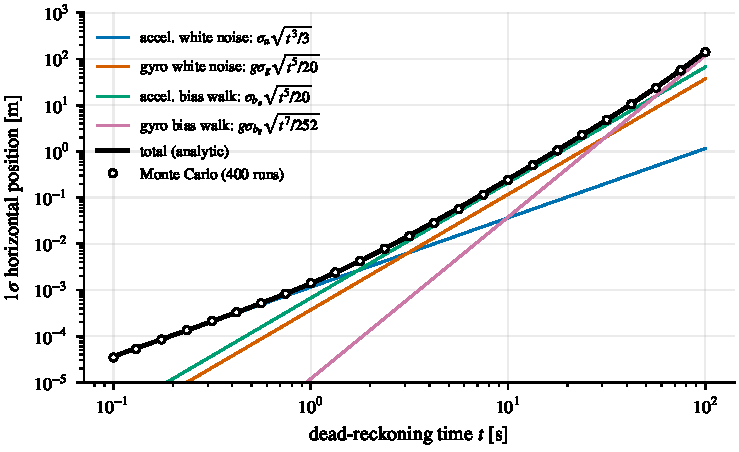
\includegraphics[width=0.88\textwidth]{fig_cov_growth.pdf}
  \caption{Horizontal position standard deviation of a dead-reckoning IMU with EuRoC noise parameters,
  from \eqref{eq:growth-laws}, with a Monte Carlo check (400 runs of the discretized error equations at
  200~Hz). Accelerometer white noise dominates for the first two seconds, the accelerometer bias walk from
  there to about a minute, and then the gyro bias walk takes over with its $t^{7/2}$ growth.}
  \label{fig:cov-growth}
\end{figure}

\begin{proposition}[Dead-reckoning growth laws]
\label{prop:growth-laws}
For a level, stationary IMU with zero initial uncertainty, the horizontal position variance grows as
\begin{equation}
  \sigma_p^2(t) = \underbrace{\frac{\sigma_a^2 t^3}{3}}_{\text{accel.\ white}}
  + \underbrace{\frac{g^2\sigma_g^2 t^5}{20}}_{\text{gyro white}}
  + \underbrace{\frac{\sigma_{b_a}^2 t^5}{20}}_{\text{accel.\ bias walk}}
  + \underbrace{\frac{g^2\sigma_{b_g}^2 t^7}{252}}_{\text{gyro bias walk}} .
  \label{eq:growth-laws}
\end{equation}
\end{proposition}
\begin{proof}
Accelerometer white noise is integrated twice ($m = 2$ in \cref{prop:integrated-noise}). Gyro white noise is integrated
once into tilt, scaled by $g$, and integrated twice more ($m = 3$). The accelerometer bias random walk is
itself integrated white noise, then integrated twice ($m = 3$). The gyro bias random walk adds one more
integration ($m = 4$). The sources are independent, so their variances add.
\end{proof}



\Cref{fig:cov-growth} evaluates \eqref{eq:growth-laws} with EuRoC's parameters. After one second of blind flight the
position uncertainty is about 1~mm, after ten seconds about 25~cm, and after a minute more than 10~m. The
camera's job is to keep the filter permanently in the left part of this plot.

\begin{projectlink}[Milestone 5]
The analytic check of M5 isolates the first term of \eqref{eq:growth-laws}: with $P_0 = 0$, only accelerometer noise and a
fixed orientation, the horizontal position variance must equal $\sigma_a^2t^3/3$. Because $\Phi$ and $Q_d$ are first-order
approximations, the agreement improves as $\Dt\to0$ (\cref{ex:double-integrator-qd}), and the test tolerance should reflect
that.
\end{projectlink}

\paragraph{Why diagonal entries need not grow monotonically.} The attitude covariance is expressed in body axes
(\cref{rem:cov-rotates}). When the vehicle rotates, the attitude block of $\Phi$ rotates the covariance between axes, so an
individual diagonal entry can shrink during pure propagation even though no information is gained. Monotonicity
holds for invariant quantities, such as the eigenvalues of $P_{\theta\theta}$ when the vehicle is not rotating, but not for
individual entries.

% ------------------------------------------------------------------------------
\section{Validating covariance propagation}

Two independent tests catch nearly all propagation bugs.

\paragraph{Finite differences on the discrete propagation.} The Jacobian of one step of the nominal integrator,
computed numerically with $\bplus/\bminus$, must match $\Phi$ column by column (the derivation exercise above). This
catches sign errors, transposes, and blocks placed at wrong indices. The test must use a non-trivial state.

\paragraph{Monte Carlo.} Simulate $M$ noisy IMU sequences from a known trajectory, integrate each with the nominal
equations from a perturbed initial state drawn from $P_0$, and compute the errors
$e^{(j)} = x_{\text{true}}\bminus\hat x^{(j)}$. Their sample covariance must agree with the propagated $P$. If the filter is
correct, the ratio of a sample variance to the predicted variance is distributed as $\chi^2_{M-1}/(M-1)$, so for
$M = 500$ it should lie in $[0.88, 1.13]$ with 95\% probability for each diagonal entry. Larger deviations, or many
entries near the bounds in the same direction, indicate an error in $G_c$, $Q_c$ or the units. This catches errors
that finite differences cannot, such as a wrong noise density or a missing $\Dt$.

\begin{takeaways}
\begin{itemize}
  \item The error state is 15-dimensional with the frozen layout $[\delta p, \delta v, \delta\theta, \delta b_a, \delta b_g]$.
  \item Error dynamics follow from substituting $x = \hat x\bplus\delta x$, subtracting the nominal dynamics, and keeping
        first-order terms. The perturbation convention changes the result.
  \item $\Phi \approx I + F_c\Dt$, $Q_d \approx G_cQ_cG_c\T\Dt$ with continuous densities; clones have identity dynamics.
  \item Position variance grows like $t^3$ (accel.\ noise), $t^5$ (gyro noise, accel.\ bias walk) and $t^7$ (gyro bias walk).
  \item Validate $\Phi$ by finite differences and $P$ by Monte Carlo with statistically justified bounds.
\end{itemize}
\end{takeaways}

\begin{exercises}
  \item Derive the velocity error dynamics for the global perturbation, and compare its structure with your local
        result. Which one depends on the vehicle's heading?
  \item Using your $F_c$, show that $\delta\theta$ is decoupled from $\delta p$ and $\delta v$, and explain this from the cascade structure.
  \item Starting from \eqref{eq:imu-discretization}, write $Q_d$ block by block and check its units.
  \item Implement covariance propagation for the 15-state system in Python and reproduce \cref{fig:cov-growth}, including
        the Monte Carlo points.
  \item For a vehicle rotating about its $z$-axis at 1~rad/s with $P_{\theta\theta} = \diag(10^{-4}, 10^{-6}, 10^{-6})$, propagate
        $P_{\theta\theta}$ for a quarter turn with no noise and observe the diagonal entries.
  \item How large must $M$ be for a Monte Carlo variance check to detect a 10\% error in $\sigma_a$ with high probability?
\end{exercises}


\part{The Error-State Filter in Practice}
\chapter{Measurement Updates, Gating and the Pose Sensor}
\label{ch:updates}
\chaptermark{Measurement Updates} % short running header

\begin{objectives}
\begin{itemize}
  \item Apply the generic manifold update to concrete sensors, deriving $H$ by the elementary Jacobians.
  \item Understand which state directions a measurement observes, from the nullspace of $H$.
  \item Implement the mock pose sensor of Milestone 6 and derive its Jacobian.
  \item Gate measurements with the $\chi^2$ test, and understand how gating fails in an overconfident filter.
  \item Understand how a pose sensor makes velocity and biases observable.
\end{itemize}
\end{objectives}

% ------------------------------------------------------------------------------
\section{The generic update}

\begin{convention}[measurement update, AGENTS.md F3]
\begin{enumerate}
  \item Residual $r = z\bminus h(\hat x)$: plain subtraction for vector measurements; for the pose measurement
        $r = [\,p_{meas} - \hat p;\ \Log_q(\hat q\inv\qprod q_{meas})\,]$.
  \item $H = \partial r/\partial\delta x$ at $\delta x = 0$ using C4 (\cref{sec:manifold-update}), derived by hand and verified by
        finite differences.
  \item $S = HPH\T + R_z$; $K = PH\T S\inv$ by a Cholesky/LDL$^\mathsf{T}$ solve, never an explicit inverse.
  \item Mahalanobis gate $r\T S\inv r < \chi^2_{0.95}(\dim r)$ from a \code{constexpr} table. Rejections are counted and
        logged, never silently dropped.
  \item Joseph form $P \gets (I - KH)P(I - KH)\T + KR_zK\T$, then injection and reset (\cref{sec:reset}).
\end{enumerate}
\end{convention}

Everything specific to a sensor is in $h$ and $H$. The rest of this section derives them for two sensors that the
project does not use, to demonstrate the technique, before turning to the pose sensor it does use.

% ------------------------------------------------------------------------------
\section{Worked example: position with a lever arm}

A GNSS antenna mounted at a known offset $\ell_b$ from the IMU, expressed in the body frame, measures the
antenna position:
\begin{equation}
  z = h(x) + n = p_{wb} + R_{wb}\,\ell_b + n, \qquad n \sim \N(0, \sigma^2I_3).
\end{equation}
The residual is a plain difference, $r = z - (\hat p + \hat R\ell_b)$. To find $H$, perturb the nominal state with
$\bplus$ and expand:
\begin{equation*}
  h(\hat x\bplus\delta x) = \hat p + \delta p + \hat R\Exp(\delta\theta)\ell_b
  \approx \hat p + \delta p + \hat R\ell_b + \hat R\sx{\delta\theta}\ell_b
  = h(\hat x) + \delta p - \hat R\sx{\ell_b}\delta\theta .
\end{equation*}
Reading off the coefficients (the rotation-action row of \cref{tab:jacobians}),
\begin{equation}
  H = \begin{bmatrix} I_3 & 0_3 & -\hat R\sx{\ell_b} & 0_3 & 0_3 \end{bmatrix}.
\end{equation}
The attitude column is non-zero because the antenna swings around the IMU when the body rotates. A
lever-arm position measurement therefore carries attitude information, but only about rotations that move
the antenna: the nullspace of $-\hat R\sx{\ell_b}$ is the direction $\ell_b$, since rotating about the lever arm itself
does not move the antenna.

% ------------------------------------------------------------------------------
\section{Worked example: a direction sensor}

A magnetometer, or an accelerometer used as an inclinometer at rest, measures a known world vector $m_w$ in
body coordinates:
\begin{equation}
  z = R_{wb}\T m_w + n .
\end{equation}
With the inverse-action row of \cref{tab:jacobians}, $h(\hat x\bplus\delta x) = \Exp(-\delta\theta)\hat R\T m_w \approx \hat R\T m_w +
\sx{\hat R\T m_w}\delta\theta$, so
\begin{equation}
  H = \begin{bmatrix} 0_3 & 0_3 & \sx{\hat R\T m_w} & 0_3 & 0_3 \end{bmatrix}.
\end{equation}
$\sx{v}$ has rank two and nullspace $\mathrm{span}(v)$, so a direction measurement observes two of the three attitude
degrees of freedom. The rotation about the measured direction is unobservable. For gravity this is the
familiar statement that an accelerometer at rest gives roll and pitch but not yaw.

\begin{keyidea}[the nullspace of $H$ tells you what a sensor cannot see]
Any error direction $\delta x \in \nullsp(H)$ produces no change in the predicted measurement, so the update cannot
correct it. Reading the nullspace of each new $H$ is a quick sanity check of both the derivation and your
intuition about the sensor.
\end{keyidea}

% ------------------------------------------------------------------------------
\section{The pose sensor of Milestone 6}

Before introducing a camera, the project tests the whole ESKF with a ``mock sensor'' that measures the pose
directly. Ground-truth poses, decimated to about 10~Hz, are corrupted with synthetic noise of known statistics.

\begin{convention}[pose measurement, AGENTS.md C6]
\begin{equation}
  p_{meas} = p_{wb} + n_p, \qquad q_{meas} = q_{wb}\qprod\Exp_q(n_\theta), \qquad
  R_z = \diag(\sigma_p^2 I_3,\ \sigma_\theta^2 I_3).
\end{equation}
\end{convention}

The attitude noise is applied on the right, in the body frame, which is exactly the local perturbation. That
choice makes the residual \eqref{eq:manifold-residual} statistically clean: if the nominal state were exact, the
attitude residual would be exactly $n_\theta$. To generate the noise, draw $n_p$ and $n_\theta$ from seeded
\code{std::mt19937\_64} generators (AGENTS.md E5) with the same $\sigma_p$, $\sigma_\theta$ that appear in $R_z$.

\begin{derivex}{the pose measurement Jacobian $H \in \R^{6\times15}$}{sol:Hpose}
Using \eqref{eq:manifold-H}, derive $H$ for $h(x) = (p_{wb}, q_{wb})$ with the residual of AGENTS.md F3.
\begin{enumerate}
  \item The position rows are a plain difference. Which state blocks does $\hat p + \delta p$ depend on?
  \item For the attitude rows, evaluate $\Log_q\big(\hat q\inv\qprod(\hat q\qprod\Exp_q(\delta\theta))\big)$ and simplify.
        Which elementary Jacobian applies if you instead linearize around a non-zero residual?
  \item Write $H$ in the frozen column order and state its nullspace. Which states are \emph{not} directly measured,
        and how can they still be corrected?
\end{enumerate}
\textbf{Check:} the finite-difference test of $r(\delta x) = h(\hat x\bplus\delta x)\bminus h(\hat x)$ at a non-trivial state, as
required by Milestone 6.
\end{derivex}

\paragraph{How unmeasured states get corrected.} The pose sensor measures neither velocity nor biases, yet the
update corrects both. The mechanism is the cross-covariance built up by propagation. Between updates, a velocity
error produces a growing position error, so $P_{pv}$ becomes large; an accelerometer bias produces a velocity error
and then a position error, so $P_{p b_a}$ grows; a gyro bias produces an attitude error, so $P_{\theta b_g}$ grows. The gain
$K = PH\T S\inv$ has non-zero rows for every state correlated with the measured ones, so each pose update corrects
them in proportion to those correlations.

\paragraph{Why the biases converge.} Observability here has an intuitive reading. The gyro bias is the slope of the
difference between the integrated gyro and the measured attitude, which a sequence of attitude measurements reveals.
The velocity is the slope of the measured position. The accelerometer bias is the difference between the
acceleration implied by successive velocities and the specific force rotated with the (measured) attitude, so it
too becomes observable. Even at rest it is separable from tilt, because the attitude is measured directly. With
pose measurements every state of the IMU error state is observable, and their covariances converge.

% ------------------------------------------------------------------------------
\section{Gating}
\label{sec:gating}

Real measurements include outliers: a misassociated feature, a reflection, a moving object. A single outlier with a
large residual can drag the estimate far away and corrupt the covariance. The $\chi^2$ test of \cref{prop:innovation}
rejects measurements that are statistically implausible given the filter's own uncertainty:
\begin{equation}
  \gamma = r\T S\inv r \ \stackrel{?}{<}\ \chi^2_{1-\alpha}(\dim r).
\end{equation}

\begin{table}[h]
\centering\small
\begin{tabular}{@{}c c c c c c c@{}}
\toprule
$\dim r$ & 1 & 2 & 3 & 4 & 5 & 6 \\
\midrule
$\chi^2_{0.95}$ & 3.841 & 5.991 & 7.815 & 9.488 & 11.070 & 12.592 \\
$\chi^2_{0.99}$ & 6.635 & 9.210 & 11.345 & 13.277 & 15.086 & 16.812 \\
\bottomrule
\end{tabular}
\caption{Gate thresholds. A longer table, up to 600 degrees of freedom, is in \cref{app:tables}.}
\label{tab:chi2-short}
\end{table}

With a 95\% gate, a consistent filter rejects 5\% of perfectly good measurements. That is the price of rejecting
most outliers, and it is why rejections are counted and logged: a rejection rate close to 5\% is a sign of
health, a rate near zero suggests an underconfident filter (or a gate that is too loose to be useful), and a
rate far above 5\% indicates overconfidence or a model error.

\begin{pitfall}[the death spiral]
Gating assumes the filter is consistent. If $P$ is too small, good measurements produce large $\gamma$ and are
rejected; with no corrections $P$ should grow, but if the model's process noise is also too small it grows slowly
while the true error grows quickly, and more measurements are rejected. The filter then dead-reckons with false
confidence until it diverges. When the rejection rate jumps, suspect overconfidence before suspecting outliers.
\end{pitfall}

The threshold depends on the dimension of $r$. A pose measurement uses $\chi^2_{0.95}(6)$, a single image
observation $\chi^2_{0.95}(2)$, and a projected MSCKF feature residual $\chi^2_{0.95}(2M-3)$, where $M$ is the number of
observations (\cref{ch:msckfupdate}). Because the quantiles grow with the dimension, the table is generated offline
and stored as a \code{constexpr} array, which avoids depending on a statistics library in the core.

% ------------------------------------------------------------------------------
\section{Pseudo-measurements and timing}

\paragraph{Pseudo-measurements.} Knowledge that is not a sensor reading can be fed to the filter as if it were one. The most useful is the \term{zero-velocity
update} (ZUPT): when the vehicle is known to be at rest (detected, for example, from a very small variance of the accelerometer and gyroscope readings over
a window), apply the measurement $z = 0 = v_{wb} + n$ with $H = [0\ \ I_3\ \ 0\ \ 0\ \ 0]$ and a small noise covariance. It stops velocity drift, and through the
correlations it also refines tilt and biases. A ZUPT applied when the vehicle is in fact moving is a large, confident, wrong measurement; the detection must
be conservative. Similar pseudo-measurements express a known constant altitude, a non-holonomic constraint (a car does not slide sideways), or a
known landmark.

\paragraph{Measurement timing.} A measurement taken at time $t_z$ must be applied to the state at $t_z$, after propagating exactly to that time
(\cref{ch:strapdown}). Measurements that arrive \emph{late}, after the filter has already propagated past their timestamp, are a problem for every filter:
either the filter buffers the IMU data and re-propagates from $t_z$, or it uses a stochastic clone of the state at $t_z$ (\cref{ch:cloning}), which is exactly the
MSCKF's approach for camera measurements. On EuRoC, data are processed offline in timestamp order, so late measurements do not occur.

% ------------------------------------------------------------------------------
\section{Testing the update}

\begin{projectlink}[Milestone 6]
The exit criteria test properties that hold for any correct implementation:
\begin{itemize}
  \item $H$ passes the finite-difference test at a non-trivial state;
  \item $P_{prior} - P_{post}$ is positive semi-definite (an update never adds uncertainty);
  \item after injection and reset all quaternions are unit, and a second update with the same $z$ produces a residual
        consistent with the first correction;
  \item as $R_z \to 0$ the posterior pose converges to $z$;
  \item with constant synthetic biases, the bias estimates converge to within their own $3\sigma$;
  \item update, injection and reset do not allocate;
  \item a full MH\_01 run with noisy ground-truth updates neither diverges nor produces NaN, and the $\chi^2$ rejection
        count is logged.
\end{itemize}
\end{projectlink}

The ``second update'' test is subtle and worth understanding. After the first update, the nominal pose has moved
toward $z$ by $K r$, so the second residual should be approximately $(I - HK)r$, which is smaller. If it is instead
larger, or has the opposite sign, the injection used the wrong side of the quaternion product or the wrong sign of
$H$.

\begin{takeaways}
\begin{itemize}
  \item Derive $H$ by perturbing $h(\hat x\bplus\delta x)$, expanding to first order and reading off coefficients.
  \item The nullspace of $H$ lists the error directions a sensor cannot see.
  \item The pose sensor's attitude noise is a local perturbation, matching the residual $\Log_q(\hat q\inv\qprod q_{meas})$.
  \item Unmeasured states are corrected through cross-covariances built up by propagation.
  \item Gate with $\chi^2_{0.95}(\dim r)$, log the rejections, and treat a high rejection rate as a symptom of overconfidence.
\end{itemize}
\end{takeaways}

\begin{exercises}
  \item For the lever-arm example, compute $S$ and $K$ for a state with
        \[ P = \diag(\sigma_p^2I,\ \sigma_v^2I,\ \sigma_\theta^2I,\ \sigma_{b_a}^2I,\ \sigma_{b_g}^2I). \]
        Which components of $\delta\theta$ does the update correct?
  \item Derive $H$ for a range measurement to a known beacon $b_w$: $z = \|p_{wb} - b_w\| + n$. What is its nullspace?
  \item Simulate the death spiral: run a 1D constant-velocity filter with $Q$ underestimated by a factor of 100 and a
        95\% gate. Plot the rejection rate and the error over time.
  \item Show that with a pose measurement of a static vehicle, the horizontal accelerometer bias is observable.
        (Hint: what does the attitude measurement remove from the tilt/bias ambiguity of \cref{ch:strapdown}?)
  \item Prove that $P_{prior} - P_{post} = KSK\T \succeq 0$ for the optimal gain, and explain why this test can fail in floating
        point if the simple covariance update is used.
\end{exercises}
% Solutions to the exercises of Chapter 18.
\begin{solutions}
  \item With $H = [\,I_3\ \ 0\ \ {-\hat R\sx{\ell_b}}\ \ 0\ \ 0\,]$ and the block-diagonal $P$, only the position and attitude blocks contribute:
        \[
          S = \sigma_p^2I + \sigma_\theta^2\hat R\sx{\ell_b}\sx{\ell_b}\T\hat R\T + \sigma^2I = \alpha\,I - \sigma_\theta^2\,(\hat R\ell_b)(\hat R\ell_b)\T,
          \qquad \alpha = \sigma_p^2 + \sigma^2 + \sigma_\theta^2\|\ell_b\|^2,
        \]
        using $\sx{\ell}\sx{\ell}\T = -\sx{\ell}^2 = \|\ell\|^2I - \ell\ell\T$. The gain blocks are $K_p = \sigma_p^2S\inv$, $K_\theta = \sigma_\theta^2(-\hat R\sx{\ell_b})\T S\inv = \sigma_\theta^2\sx{\ell_b}\hat R\T S\inv$,
        and zero for velocity and biases. Since $S\inv(\hat R\ell_b) \propto \hat R\ell_b$ and $\sx{\ell_b}\hat R\T\hat R\ell_b = 0$, the attitude gain simplifies to
        \[
          K_\theta = \frac{\sigma_\theta^2}{\sigma_p^2 + \sigma^2 + \sigma_\theta^2\|\ell_b\|^2}\,\sx{\ell_b}\hat R\T .
        \]
        Its range is the range of $\sx{\ell_b}$: the update corrects only the attitude components perpendicular to the lever arm, never the rotation
        about $\ell_b$ itself, which does not move the antenna. Velocity and biases are not corrected here because this prior has no cross-covariances;
        after some propagation they would be.

  \item With $h(x) = \|p - b_w\|$ and $\hat\rho = \|\hat p - b_w\|$, perturbing $p = \hat p + \delta p$ gives $h \approx \hat\rho + u\T\delta p$ with $u = (\hat p - b_w)/\hat\rho$, so
        \[
          H = [\,u\T\ \ 0\ \ 0\ \ 0\ \ 0\,] \in \R^{1\times15} .
        \]
        Its nullspace is 14-dimensional: the two position directions perpendicular to the line of sight (moving on the sphere around the beacon), and
        all velocity, attitude and bias errors. One range observes one number; position perpendicular to the line of sight becomes observable only
        through several beacons or through motion and the correlations it builds.

  \item Simulate a constant-velocity target (acceleration density $\sqrt{0.5}$, position measurements at 10~Hz with unit variance) and run the
        filter with $Q$ divided by 100 and a $\chi^2_{0.95}(1)$ gate. Typical results, per 30-second window:
        \begin{center}\small
        \begin{tabular}{@{}l l l@{}}
        \toprule
        filter & rejection rate & RMS position error \\
        \midrule
        correct $Q$, gated & 2--8\% & 0.4--0.65~m \\
        $Q/100$, gated & 79\%, then 100\% & 26, 126, 243, \dots, 3246~m \\
        $Q/100$, not gated & 0\% & 0.8--1.7~m \\
        \bottomrule
        \end{tabular}
        \end{center}
        The overconfident filter predicts innovations that are far too small, so good measurements fail the gate; each rejection removes the
        correction the filter needed, the error grows, more measurements are rejected, and within half a minute the filter ignores all data and
        dead-reckons. Its reported $\sigma$ (about 200~m at the end) stays far below its actual error. Without the gate the same mistuned filter is
        merely suboptimal: its error stays bounded. A rejection rate far above the design value is the alarm signal (\cref{sec:gating}).

  \item At rest, the accelerometer measures $\hat R\T(-g_w) + b_a$, and to first order a tilt error and a horizontal bias change this reading in the same way:
        in the velocity error dynamics both enter through the horizontal specific-force error, so from accelerations alone only their combination is
        observable (\cref{ch:strapdown}). With a pose sensor, the position measurements make the velocity error and its rate observable (two
        differentiations, as in \cref{sec:observability-linear}), while the attitude measurement observes $\delta\theta$ directly. The rate of the velocity
        error is (tilt term) $+$ (bias term); with the tilt term known from the attitude measurement, the bias term, and hence the horizontal bias, is
        determined. The vertical bias was observable already (it changes the measured magnitude of gravity, which the position measurements expose),
        and the gyro bias is observable from the drift of the attitude between measurements. With a pose sensor, every IMU state is observable,
        which is why the covariances converge in Milestone 6.

  \item For the optimal gain, $P_{\mathrm{prior}} - P_{\mathrm{post}} = KHP = KSK\T$ (\cref{thm:kf-update}), and $KSK\T \succeq 0$ because it is a congruence of $S \succ 0$
        (\cref{prop:psd}). In floating point the simple update $P_{\mathrm{post}} = (I - KH)P$ is neither symmetric nor guaranteed PSD (Exercise 12.3), and
        $P_{\mathrm{prior}} - P_{\mathrm{post}}$ then has rounding-level asymmetry and can have slightly negative eigenvalues, notably in directions the
        measurement does not observe, where the true difference is exactly zero and the computed one is $\pm u\|P\|$. A test must therefore symmetrize the
        difference and allow a tolerance: $\lambda_{\min}\big(\tfrac12(D + D\T)\big) \ge -c\,u\,\|P\|$ with a small constant $c$. Using the Joseph form and
        symmetrizing after each update makes $P_{\mathrm{post}}$ itself PSD, but the difference still needs the tolerance.
\end{solutions}


\chapter{Consistency and Evaluation}
\label{ch:consistency}

\begin{objectives}
\begin{itemize}
  \item Test whether a filter's covariance tells the truth, with NEES, NIS and $3\sigma$ coverage.
  \item Compute exact statistical bounds for single-run and Monte Carlo tests.
  \item Diagnose over- and under-confidence and tune noise parameters without cheating.
  \item Measure trajectory accuracy with ATE and RPE, using the alignment appropriate for VIO.
\end{itemize}
\end{objectives}

A filter produces two things: an estimate and a covariance. Most evaluations look only at the first. But a
filter with good average accuracy and a covariance that is too small is dangerous: it rejects valid measurements,
it reports false confidence to whatever consumes its output, and it eventually diverges. This chapter is about
checking the second output.

% ------------------------------------------------------------------------------
\section{What consistency means}

Recall from \cref{ch:prob} that a filter reporting $(\hat x_k, P_k)$ is consistent if its error $e_k = x_k\bminus\hat x_k$ has
zero mean and covariance $P_k$. Together with \cref{prop:innovation}, a consistent, correctly modeled filter
satisfies three testable properties:
\begin{enumerate}
  \item estimation errors are compatible with $P_k$ (tested with NEES, needs ground truth);
  \item innovations are compatible with $S_k$ (tested with NIS, needs no ground truth);
  \item innovations are white (tested with autocorrelation, needs no ground truth).
\end{enumerate}
The error must be computed with the manifold difference $\bminus$, using exactly the same convention as the
filter's covariance. Comparing a local-perturbation covariance with a global attitude error, or with an Euler
angle difference, produces meaningless statistics.

% ------------------------------------------------------------------------------
\section{Normalized estimation error squared}

\begin{definition}[NEES]
The normalized estimation error squared at time $k$ is
\begin{equation}
  \epsilon_k = e_k\T P_k\inv e_k, \qquad e_k = x_k\bminus\hat x_k .
\end{equation}
\end{definition}

If the filter is consistent and its errors are Gaussian, $\epsilon_k \sim \chi^2_n$ with $n = \dim e$ by
\cref{thm:mahalanobis-chi2}: its expected value is $n$. A single run gives one sample per time step, which is noisy.
Monte Carlo runs average it out. With $N$ independent runs, the average NEES
$\bar\epsilon_k = \frac1N\sum_{j=1}^N\epsilon_k^{(j)}$ satisfies $N\bar\epsilon_k \sim \chi^2_{Nn}$, so the two-sided 95\% interval is
\begin{equation}
  \left[\ \frac{\chi^2_{0.025}(Nn)}{N},\ \frac{\chi^2_{0.975}(Nn)}{N}\ \right].
  \label{eq:anees-bounds}
\end{equation}
For the 15-state IMU filter with $N = 50$ runs this is $[13.52, 16.56]$; for $N = 100$, $[13.95, 16.09]$.
\Cref{app:tables} lists more. Average NEES above the interval means overconfidence (errors larger than claimed);
below means underconfidence.

\begin{figure}[t]
  \centering
  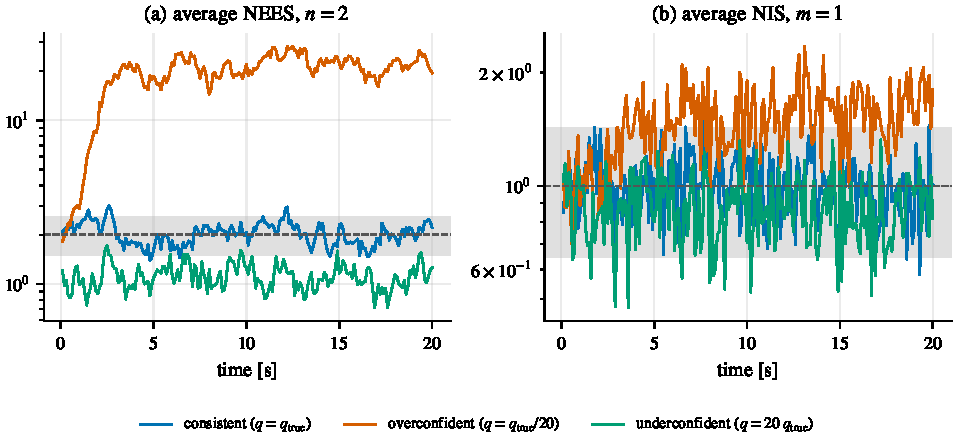
\includegraphics[width=\textwidth]{fig_nees.pdf}
  \caption{Consistency statistics of a constant-velocity filter over 50 Monte Carlo runs, with the 95\%
  acceptance region (gray) of \eqref{eq:anees-bounds}. Underestimating the process noise by a factor of 20 makes the
  filter overconfident: the NEES leaves the region by an order of magnitude, and the NIS rises above it. Overestimating
  it makes the filter underconfident: the NEES falls below the region. Note that the NIS of the underconfident filter
  is less clearly abnormal: NIS alone is a weak detector of underconfidence.}
  \label{fig:nees}
\end{figure}

\paragraph{Block NEES.} The NEES of the full state mixes well-estimated and poorly estimated blocks. Computing it
separately for position, velocity, attitude and biases, each with its own $3\times3$ block of $P$ and $\chi^2_3$ bounds, points
directly at the misbehaving part.

% ------------------------------------------------------------------------------
\section{Normalized innovation squared}

\begin{definition}[NIS]
$\nu_k = r_k\T S_k\inv r_k$, the same quantity the gate computes.
\end{definition}

Under consistency $\nu_k \sim \chi^2_m$ with $m = \dim r_k$. NIS needs no ground truth, so it is the main consistency
monitor on real data. Two summaries are useful: the fraction of updates with $\nu_k$ below its 95\% quantile, which
should be close to 95\% (Milestone 7), and the time-average of $\nu_k$, which should be close to $m$. If measurements have
different dimensions, normalize by $m_k$ or compare each against its own quantile.

\paragraph{$3\sigma$ coverage.} For each scalar component $i$, a consistent Gaussian error lies within $\pm3\sqrt{P_{ii}}$
99.7\% of the time. Plotting errors against their $3\sigma$ envelopes is the most readable diagnostic, and the coverage
fraction is a simple scalar summary. On EuRoC, Milestone 7 requires at least 95\% coverage for velocity and biases.
These states are not measured by the pose sensor, so their consistency is not circular.

% ------------------------------------------------------------------------------
\section{Diagnosing inconsistency}

\begin{table}[t]
\centering\small
\begin{tabularx}{\textwidth}{@{}l l X@{}}
\toprule
\textbf{NEES} & \textbf{NIS} & \textbf{Likely causes} \\
\midrule
high & high & process noise too small; wrong noise units (missing $\Dt$ or $\sqrt{\Dt}$); unmodeled IMU errors; integration error \\
high & normal & errors in directions the measurement does not see (unobservable states, e.g.\ yaw in VIO); wrong $\bminus$ convention in the evaluation \\
normal & high & measurement noise too small; outliers passing the gate; wrong $H$ \\
low & low & process or measurement noise too large \\
high, growing & normal & spurious information along unobservable directions (EKF inconsistency, \cref{ch:observability}) \\
spikes & spikes & time-synchronization errors; wrong extrinsics; bad initialization \\
\bottomrule
\end{tabularx}
\caption{Reading consistency statistics. Combinations narrow the search for the bug.}
\label{tab:consistency-diagnosis}
\end{table}

\Cref{tab:consistency-diagnosis} is a starting point for debugging. Two additional checks are valuable. First, plot each
residual component over time: a non-zero mean reveals a bias (wrong extrinsics, a wrong sign in $h$); slow oscillation
reveals correlated errors (a coloured noise the filter assumes white). Second, compare the covariance with Monte
Carlo statistics on synthetic data, where the truth is known exactly and the noise is exactly as modeled. If the filter
is inconsistent on synthetic data, the bug is in the filter. If it is consistent there but not on real data, the problem is
the model.

\subsection{Tuning without cheating}

\begin{enumerate}
  \item \textbf{Synthetic first.} With synthetic data generated with exactly the filter's noise parameters, there is
        nothing to tune: a consistent implementation must pass. Any failure is a bug.
  \item \textbf{Physically meaningful knobs only.} On real data, adjust the IMU noise densities (start from
        \cref{tab:euroc-imu}, inflate modestly for unmodeled effects) and the measurement noise (start from the pixel
        noise of the detector). Do not add arbitrary noise to arbitrary states.
  \item \textbf{Judge on consistency, not accuracy.} Choose parameters that make NIS and coverage statistics correct.
        Lower trajectory error obtained by making the filter inconsistent will not generalize.
  \item \textbf{Separate tuning from evaluation.} Tune on some sequences and report results on others.
  \item \textbf{Ground truth never enters the filter} except where explicitly allowed and logged (initialization).
\end{enumerate}

% ------------------------------------------------------------------------------
\section{Trajectory accuracy}

Consistency says whether the covariance is honest; accuracy says how small the errors are. VIO accuracy is
reported with two metrics~\cite{sturm2012tum, zhang2018tutorial}.

\subsection{Absolute trajectory error}

The estimated trajectory lives in a world frame that is only defined up to the unobservable directions, so it must
be aligned with the ground truth before comparing. Given time-associated positions $p_i$ (ground truth) and
$\hat p_i$ (estimate), find the transformation that best maps the estimate onto the truth, then compute
\begin{equation}
  \mathrm{ATE}_{\mathrm{RMSE}} = \Big(\frac1N\sum_{i=1}^N\big\|p_i - (R^\star\hat p_i + t^\star)\big\|^2\Big)^{1/2}.
\end{equation}
For rigid alignment, the optimal transformation has a closed form (Kabsch/Umeyama~\cite{umeyama1991}).

\begin{proposition}[Optimal rigid alignment]
\label{prop:umeyama}\label{sec:umeyama}
\index{Umeyama alignment}
Let $\mu$ and $\hat\mu$ be the means of the two point sets, $a_i = p_i - \mu$ and $b_i = \hat p_i - \hat\mu$ the centered points, and
$\Sigma_{ab} = \frac1N\sum_ia_ib_i\T = UDV\T$ an SVD. The minimizer of $\sum_i\|p_i - (R\hat p_i + t)\|^2$ over rotations $R$ and translations $t$ is
\begin{equation}
  R^\star = U\diag\big(1, 1, \det(UV\T)\big)V\T, \qquad t^\star = \mu - R^\star\hat\mu .
\end{equation}
\end{proposition}
\begin{proof}
For fixed $R$, the cost is a quadratic in $t$ minimized where its gradient vanishes, $\sum_i(p_i - R\hat p_i - t) = 0$, i.e.\ $t = \mu - R\hat\mu$: the alignment maps
centroid onto centroid. Substituting, the cost becomes $\sum_i\|a_i - Rb_i\|^2 = \sum_i(\|a_i\|^2 + \|b_i\|^2) - 2\sum_ia_i\T Rb_i$, so we must maximize
$\sum_ia_i\T Rb_i = \tr\big(R\sum_ib_ia_i\T\big) = N\tr(R\,VDU\T) = N\tr(D\,Z)$ with $Z = U\T RV$. $Z$ is orthogonal, so its diagonal entries are at most one in
magnitude, and $\tr(DZ) = \sum_id_iZ_{ii} \le \sum_id_i$, with equality for $Z = I$, i.e.\ $R = UV\T$. If $\det(UV\T) = -1$ this is a reflection, not a rotation; the
best rotation then flips the axis with the smallest singular value, $Z = \diag(1, 1, -1)$, which gives the stated formula.
\end{proof}

If the scale is also free (a similarity transform, needed for monocular vision without an IMU), the optimal scale is
$s^\star = \tr(D\,\diag(1, 1, \det(UV\T)))\big/\frac1N\sum_i\|b_i\|^2$, applied as $s^\star R^\star\hat p_i + t^\star$ with $t^\star = \mu - s^\star R^\star\hat\mu$.

\begin{keyidea}[align only what is unobservable]
Which transformation to allow depends on the estimator. Monocular vision alone has a free scale, so it uses a
similarity transform (7 DOF). VIO has metric scale and observable roll and pitch: its unobservable directions are
exactly translation and yaw. The appropriate alignment is therefore 4-DOF (translation plus a rotation about
gravity)~\cite{zhang2018tutorial}. A full 6-DOF alignment would also remove roll and pitch errors that the
estimator was responsible for.
\end{keyidea}

The 4-DOF alignment follows the same proof with $R$ restricted to rotations $R_z(\psi)$ about the vertical. For centered points $a = (x, y, z)$ (truth)
and $b = (\hat x, \hat y, \hat z)$ (estimate), $a\T R_z(\psi)b = (x\hat x + y\hat y)\cos\psi + (y\hat x - x\hat y)\sin\psi + z\hat z$, whose sum over the points is maximized by
\begin{equation}
  \psi^\star = \atantwo\Big(\sum_i(y_i\hat x_i - x_i\hat y_i),\ \sum_i(x_i\hat x_i + y_i\hat y_i)\Big),
  \label{eq:4dof-yaw}
\end{equation}
again with $t^\star = \mu - R_z(\psi^\star)\hat\mu$.

Milestone 10b reports ATE after SE(3) alignment, as in most published benchmarks; reporting the 4-DOF result
alongside it is more faithful to what VIO can know.

\subsection{Relative pose error}

ATE is dominated by the largest drift and depends on trajectory length and shape. The relative pose error (RPE)
compares relative motions over a fixed distance or time $\Delta$:
\begin{equation}
  E_i = \big(T_{i}\inv T_{i+\Delta}\big)\inv\big(\hat T_i\inv\hat T_{i+\Delta}\big),
\end{equation}
and reports statistics of the translation and rotation parts of $E_i$, often as a percentage of distance traveled. It
needs no global alignment and measures local drift, which is what odometry is about. The \code{evo}
package~\cite{grupp2017evo} computes both metrics with all the alignment variants.

\begin{projectlink}[Milestone 7]
M7 logs $\hat x$, $\diag(P)$, ground truth, NIS and NEES to a preallocated buffer, flushes it outside the hot loop, and
plots $3\sigma$ envelopes and NEES/NIS against their $\chi^2$ bounds from a single script. Exit criteria: average NEES inside
the 95\% interval for 15 DOF over most of a $\geq50$-run synthetic Monte Carlo; NIS within its per-update bound for about
95\% of updates; at least 95\% $3\sigma$ coverage of velocity and biases on MH\_01; zero allocations while logging.
\end{projectlink}

\begin{takeaways}
\begin{itemize}
  \item A filter must be judged on the honesty of its covariance as well as its accuracy.
  \item NEES needs ground truth and tests $P$; NIS needs none and tests $S$. Both are $\chi^2$ under consistency.
  \item Monte Carlo averages have exact bounds $[\chi^2_{0.025}(Nn), \chi^2_{0.975}(Nn)]/N$.
  \item Overconfidence (NEES too high) is the dangerous failure; NIS alone detects underconfidence poorly.
  \item Tune physically meaningful parameters for consistency, on synthetic data first.
  \item Report ATE after an alignment matched to the unobservable directions, and RPE for local drift.
\end{itemize}
\end{takeaways}

\begin{exercises}
  \item Show that the single-run NEES of a consistent 15-state filter exceeds its 95\% quantile 5\% of the time. Why
        is the Monte Carlo average a much sharper test?
  \item Reproduce \cref{fig:nees}. Then make only the measurement noise wrong instead of the process noise and compare
        the signatures.
  \item Derive the closed-form 4-DOF alignment above by maximizing $\sum_i p_i\T R_z(\psi)\hat p_i$ over $\psi$.
  \item Explain why the NEES of yaw in a VIO run on real data tends to grow over time even when the NIS looks
        healthy. (Revisit after \cref{ch:observability}.)
  \item Compute the RPE over 10~m segments for a trajectory with a constant yaw drift of $1^\circ$ per minute flying at
        1~m/s. How does it compare with the ATE after a 10-minute flight?
\end{exercises}
% Solutions to the exercises of Chapter 19.
\begin{solutions}
  \item If the filter is consistent and its errors Gaussian, $\epsilon_k = e_k\T P_k\inv e_k \sim \chi^2_{15}$ (\cref{thm:mahalanobis-chi2}). The 95\% quantile $\chi^2_{0.95}(15) = 25.0$ is
        by definition the value exceeded with probability 5\%, so a single run exceeds it at 5\% of its time steps. A single sample is a weak test:
        its two-sided 95\% range is $[6.3, 27.5]$, a factor of more than four, and a filter whose covariance is too small by 30\% still produces values
        inside it most of the time. Averaging over $N$ independent runs shrinks the spread: $N\bar\epsilon \sim \chi^2_{15N}$ has relative standard deviation
        $\sqrt{2/(15N)}$, and for $N = 50$ the interval is $[13.5, 16.6]$, about $\pm10\%$. A 30\% error now moves the average far outside it.

  \item In a simulation of the same kind as \cref{fig:nees} ($q = r = 1$, 50 runs of 200 steps), the average NEES ($n = 2$) and NIS ($m = 1$) after the
        transient are:
        \begin{center}\small
        \begin{tabular}{@{}l c c@{}}
        \toprule
        filter & NEES (band $[1.48, 2.59]$) & NIS (band $[0.65, 1.43]$) \\
        \midrule
        consistent & 1.9 & 1.00 \\
        $Q/20$ & 20.0 & 1.5 \\
        $20\,Q$ & 1.1 & 0.87 \\
        $R/20$ & 21.7 & 17.5 \\
        $20\,R$ & 1.0 & 0.08 \\
        \bottomrule
        \end{tabular}
        \end{center}
        Both kinds of error make the filter over- or underconfident in the NEES, but the NIS separates them. A wrong measurement noise enters $S$
        directly, so the NIS is wildly off ($17.5$ and $0.08$). A wrong process noise affects $S$ only through $HP^-H\T$, which the measurement noise partly
        masks, so the NIS moves much less ($1.5$ and $0.87$, the latter inside the band). Rule of thumb: NIS problems point at $R$ (or at outliers and
        wrong measurement models), NEES problems with a healthy NIS point at $Q$ or at unobservable directions (\cref{tab:consistency-diagnosis}).

  \item With centered points $a_i = (x_i, y_i, z_i)$ (truth) and $b_i = (\hat x_i, \hat y_i, \hat z_i)$ (estimate),
        \[
          \sum_ia_i\T R_z(\psi)b_i = \cos\psi\underbrace{\sum_i(x_i\hat x_i + y_i\hat y_i)}_{A} + \sin\psi\underbrace{\sum_i(y_i\hat x_i - x_i\hat y_i)}_{B} + \sum_iz_i\hat z_i .
        \]
        As a function of $\psi$ this is $\sqrt{A^2 + B^2}\cos(\psi - \psi_0) + \text{const}$ with $(\cos\psi_0, \sin\psi_0) \propto (A, B)$, so it is maximized at
        $\psi^\star = \atantwo(B, A)$, which is \eqref{eq:4dof-yaw}. (Setting the derivative $-A\sin\psi + B\cos\psi$
        to zero gives $\tan\psi = B/A$, which has two solutions; the $\atantwo$ picks the maximum rather than the minimum.) The translation follows
        as before: $t^\star = \mu - R_z(\psi^\star)\hat\mu$, which maps centroid onto centroid.

  \item The standard EKF linearizes at estimates that change over time, which makes the global yaw appear observable in its linearized model
        (\cref{ch:observability}). The filter then extracts spurious yaw information from measurements that contain none: its yaw variance shrinks,
        or grows more slowly than the true yaw error, which in VIO drifts like a random walk because nothing measures it. The NEES of yaw,
        $e_\psi^2/\sigma_\psi^2$, therefore grows steadily. The NIS stays healthy because innovations depend only on observable quantities (relative motion,
        roll, pitch, scale): an error along an unobservable direction changes no predicted measurement, so it cannot show up in the residuals
        (\cref{tab:consistency-diagnosis}, ``high, growing / normal'').

  \item A yaw drift of $1^\circ$ per minute is $\omega_d = 2.9\times10^{-4}$~rad/s. A 10~m segment takes 10~s at 1~m/s, during which the heading drifts by
        $0.167^\circ$: that is the rotational RPE. The translational RPE is the lateral offset accumulated within the segment, about
        $\tfrac12\omega_dv\,\Delta t^2 = 1.5$~cm (a simulation gives $1.4$~cm), i.e.\ $0.15\%$ of the distance travelled, and it is the same for every segment of the
        flight. For a straight 10-minute flight, by contrast, the estimated path bends into an arc of radius $v/\omega_d = 3.4$~km: the final position error is
        $\tfrac12\omega_dvT^2 = 52$~m, the RMS error without alignment 23~m, and after the best rigid alignment still $3.9$~m. The ATE grows quadratically
        with the duration and depends on the trajectory and on the alignment; the RPE does not grow and measures the drift rate itself, which is why
        odometry is compared with RPE and full trajectories with ATE.
\end{solutions}



\part{Computer Vision}
\chapter{Image Formation and Camera Models}
\label{ch:camera}
\chaptermark{Image Formation} % short running header

\begin{objectives}
\begin{itemize}
  \item Understand how a camera forms an image: pinholes, lenses, focus, sensors, exposure and shutters.
  \item Derive the pinhole projection, the intrinsic matrix and normalized image coordinates.
  \item Use homogeneous coordinates and the basic projective geometry of points, lines and homographies.
  \item Model and invert the radial-tangential lens distortion used by EuRoC, and know the fisheye alternative.
  \item Understand how cameras are calibrated.
  \item State the project's camera measurement model with its noise, derive the projection Jacobian, and understand extrinsics and time offsets.
\end{itemize}
\end{objectives}

% ==============================================================================
\section{How a camera forms an image}

\subsection{From pinhole to lens}

A camera measures the \emph{directions} of light rays. In a \emph{camera obscura}, light from the scene enters a dark box through a tiny hole and
forms an inverted image on the opposite wall: every point of the wall receives light only from the scene point on the straight line through the
hole. This is the \term{pinhole model}, and it is geometrically perfect. It is also impractical: a hole small enough to give a sharp image lets in
very little light.

A lens gathers light through a large aperture and bends it so that all rays from one scene point converge again at one image point. For an ideal
\emph{thin lens} of focal length $f_L$, a point at distance $z_o$ in front of the lens is imaged sharply at distance $z_i$ behind it, where
\begin{equation}
  \frac1{f_L} = \frac1{z_o} + \frac1{z_i} .
\end{equation}
For distant scenes ($z_o \gg f_L$) the image forms at $z_i \approx f_L$, which is where the sensor sits in a camera focused at infinity. Points at other
distances form slightly blurred spots; the range of distances that stays acceptably sharp is the \emph{depth of field}, larger for small apertures and
short focal lengths. The central ray through the lens center is not bent, so the geometry of a focused lens camera is exactly that of a pinhole at
the lens center: the pinhole model describes it, and lens imperfections are added as \emph{distortion} (\cref{sec:distortion}).

\subsection{The image sensor}

The sensor is a grid of light-sensitive \emph{pixels}. Each accumulates charge in proportion to the light it receives during the \emph{exposure time},
and the charge is converted into a number, typically 8 bits per pixel for the monochrome cameras of EuRoC. Several properties of the sensor matter to an
estimator.
\begin{itemize}
  \item \emph{Exposure and motion blur.} A camera rotating at $\omega$ rad/s during an exposure of $T$ seconds smears each point over about $f\omega T$ pixels, with
        $f$ the focal length in pixels. At 1~rad/s, 5~ms and $f = 458$~px this is 2.3~px, enough to degrade feature tracking. EuRoC's difficult
        sequences contain exactly such blur.
  \item \emph{Global versus rolling shutter.} A global shutter exposes all pixels at the same instant, as EuRoC's cameras do. A rolling shutter (common in
        phones) exposes rows one after another, so each row is captured at a different time and, on a moving camera, from a different pose. Rolling-shutter
        images need an extended measurement model.
  \item \emph{Noise and dynamic range.} Pixel values carry photon and electronic noise, and scenes brighter or darker than the sensor's range saturate. Auto
        exposure changes the brightness of the same scene point between frames, which matters for intensity-based tracking (\cref{ch:frontend}).
\end{itemize}

\paragraph{Pixel coordinates.} We write pixel coordinates as $(u, v)$, with $u$ increasing to the right and $v$ increasing downward, and the origin at the
top-left of the image. In OpenCV's convention, integer coordinates are pixel \emph{centers}. The camera frame $C$ is aligned with this: $x_c$ to the right, $y_c$
down, $z_c$ along the optical axis into the scene.

% ==============================================================================
\section{The pinhole projection}

An ideal pinhole camera lets light through a single point, the optical center. A scene point with camera-frame coordinates $p_c = (X, Y, Z)$, with $Z$ along the
optical axis, projects through the center onto an image plane. Placing a virtual image plane at unit distance \emph{in front of} the center (which avoids
the inversion of the physical image) and using similar triangles, the image of the point is
\begin{equation}
  \pi(p_c) = \begin{bmatrix} x \\ y \end{bmatrix} = \begin{bmatrix} X/Z \\ Y/Z \end{bmatrix}.
  \label{eq:pinhole}
\end{equation}
These are the \term{normalized image coordinates}: dimensionless, independent of the lens, and equal to the tangents of the ray's angles from the optical axis.
The vector $\bar x = (x, y, 1)$ is the \term{bearing} of the point, defined up to scale.

\begin{figure}[t]
\centering
\begin{tikzpicture}[scale=1.0]
  \coordinate (O) at (0,0);
  \draw[frameaxis, plotblue] (O) -- (6.2,0) node[right] {$z_c$ (optical axis)};
  \draw[frameaxis, plotorange] (O) -- (0,-1.6) node[below] {$y_c$};
  \fill (O) circle (1.6pt) node[above left] {$C$};
  \draw[thick, primary] (2,1.8) -- (2,-1.4);
  \node[primary, font=\footnotesize, align=center] at (2,2.15) {normalized plane $Z = 1$};
  \coordinate (P) at (5.6,-1.25);
  \fill[plotgreen] (P) circle (2pt) node[right] {$p_c = (X, Y, Z)$};
  \draw[plotgreen, dashed] (O) -- (P);
  \coordinate (I) at (2,{-1.25*2/5.6});
  \fill[conv] (I) circle (1.8pt);
  \node[conv, font=\footnotesize, right] at (2.05,-0.18) {$y = Y/Z$};
  \draw[<->, black!60] (0,0.5) -- (2,0.5) node[midway, above, font=\footnotesize] {$1$};
  \draw[<->, black!60] (0,0.95) -- (5.6,0.95) node[midway, above, font=\footnotesize] {$Z$};
\end{tikzpicture}
\caption{Pinhole projection in the $y$-$z$ plane. The ray from the optical center $C$ to the point intersects the plane $Z = 1$ at height $Y/Z$. All points
along the ray project to the same image point, so depth is lost.}
\label{fig:pinhole}
\end{figure}

\subsection{Intrinsic parameters}

Pixels are obtained by scaling and shifting the normalized coordinates with the \term{intrinsic matrix}:
\begin{equation}
  \begin{bmatrix} u \\ v \\ 1 \end{bmatrix} = K\begin{bmatrix} x \\ y \\ 1 \end{bmatrix}, \qquad
  K = \begin{bmatrix} f_u & s & c_u \\ 0 & f_v & c_v \\ 0 & 0 & 1 \end{bmatrix},
\end{equation}
with focal lengths $f_u, f_v$ in pixels, principal point $(c_u, c_v)$ (where the optical axis pierces the image), and skew $s$ (zero for modern sensors). The
focal length in pixels is the physical focal length divided by the pixel pitch; $f_u \neq f_v$ if pixels are not square. Inverting $K$ turns a pixel into a bearing,
$\bar x = K\inv(u, v, 1)\T$. The horizontal \emph{field of view} of a $W$-pixel-wide image is $2\arctan\big(W/(2f_u)\big)$, ignoring distortion. EuRoC's \code{cam0} has
$f_u = 458.654$, $f_v = 457.296$, $c_u = 367.215$, $c_v = 248.375$ on a $752\times480$ sensor: a horizontal field of view of about $79^\circ$.

% ==============================================================================
\section{Homogeneous coordinates and projective geometry}
\label{sec:homogeneous}

\subsection{Points and lines in the image}

\index{homogeneous coordinates}
The image point $(x, y)$ corresponds to the whole ray of 3D vectors $\lambda(x, y, 1)$, $\lambda \ne 0$. \term{Homogeneous coordinates} make this explicit: a point of the
plane is represented by any non-zero 3-vector $\tilde x = (x_1, x_2, x_3)$, with $\tilde x$ and $\lambda\tilde x$ representing the same point, and the ordinary coordinates
are recovered as $(x_1/x_3, x_2/x_3)$. Vectors with $x_3 = 0$ represent \emph{points at infinity}: directions, where parallel lines meet.

A line $ax + by + c = 0$ is represented by the 3-vector $l = (a, b, c)$, also up to scale, and a point lies on it exactly when
\begin{equation}
  l\T\tilde x = 0 .
\end{equation}
This symmetric relation makes two constructions one-liners:
\begin{itemize}
  \item the line through two points is $l = \tilde x_1\times\tilde x_2$ (it is orthogonal to both, so both lie on it);
  \item the intersection of two lines is $\tilde x = l_1\times l_2$ (by the same argument).
\end{itemize}
Two parallel lines $(a, b, c_1)$ and $(a, b, c_2)$ intersect at $(b, -a, 0)$ times a constant: a point at infinity in their common direction. In an image of a
3D scene, parallel 3D lines are generally not parallel in the image and meet at a finite \emph{vanishing point}, the image of their common direction.

\subsection{Homographies}

\begin{definition}[Homography]
\index{homography}
A \term{homography} (projective transformation) of the plane is a map $\tilde x \mapsto H\tilde x$ for an invertible $3\times3$ matrix $H$, defined up to scale (eight
degrees of freedom).
\end{definition}

Homographies map lines to lines (if $l\T\tilde x = 0$ then $(H\mT l)\T(H\tilde x) = 0$) but do not preserve parallelism, lengths or angles. Two situations in
which they arise are central to vision:
\begin{itemize}
  \item the images of a \emph{plane} in two views are related by a homography (\cref{ch:multiview}), which is the basis of camera calibration below;
  \item two images taken by a camera that only \emph{rotates} are related by the homography $KRK\inv$, independently of the scene (\cref{ch:multiview,ch:frontend}).
\end{itemize}

\subsection{The projection matrix}

In homogeneous coordinates the complete projection of a world point $p_w$ (with homogeneous coordinates $\tilde p_w = (p_w, 1)$) into pixels is a single linear map,
\begin{equation}
  \lambda\begin{bmatrix} u \\ v \\ 1\end{bmatrix} = K\begin{bmatrix} R_{cw} & p_{cw}\end{bmatrix}\tilde p_w = P\,\tilde p_w,
  \qquad P = K\,[R_{cw}\ \ p_{cw}] \in \R^{3\times4},
\end{equation}
where $(R_{cw}, p_{cw})$ maps world coordinates into the camera frame and $\lambda = Z$ is the depth. The \emph{camera matrix} $P$ has eleven degrees of freedom (twelve
entries up to scale): five intrinsic and six extrinsic. Linear methods that estimate $P$, $H$ or the essential matrix from correspondences
(\cref{ch:multiview}) all exploit the fact that projection is linear in homogeneous coordinates.

% ==============================================================================
\section{Lens distortion}
\label{sec:distortion}

Real lenses bend rays, most strongly near the image edges, so the image of a straight line is curved. The \term{radial-tangential} (Brown--Conrady) model
used by EuRoC maps ideal normalized coordinates $(x, y)$ to distorted ones $(x_d, y_d)$:
\begin{align}
  x_d &= x\,(1 + k_1r^2 + k_2r^4) + 2p_1xy + p_2(r^2 + 2x^2), \\
  y_d &= y\,(1 + k_1r^2 + k_2r^4) + p_1(r^2 + 2y^2) + 2p_2xy, \qquad r^2 = x^2 + y^2,
\end{align}
after which $K$ is applied to $(x_d, y_d)$. The \emph{radial} terms ($k_1, k_2$) model the dominant symmetric distortion of a lens; the \emph{tangential} terms ($p_1, p_2$)
model a lens slightly tilted or decentered relative to the sensor. For \code{cam0}, $(k_1, k_2, p_1, p_2) = (-0.2834, 0.07396, 1.94\times10^{-4}, 1.76\times10^{-5})$. The negative
$k_1$ produces \emph{barrel} distortion (\cref{fig:distortion}). At the middle of the left and right image edges the radial factor $1 + k_1r^2 + k_2r^4$ is about $0.79$,
which moves points by about 100 pixels; at the corners it is about $0.73$, a shift of about 160 pixels. Ignoring distortion is therefore not an option.

\begin{figure}[t]
  \centering
  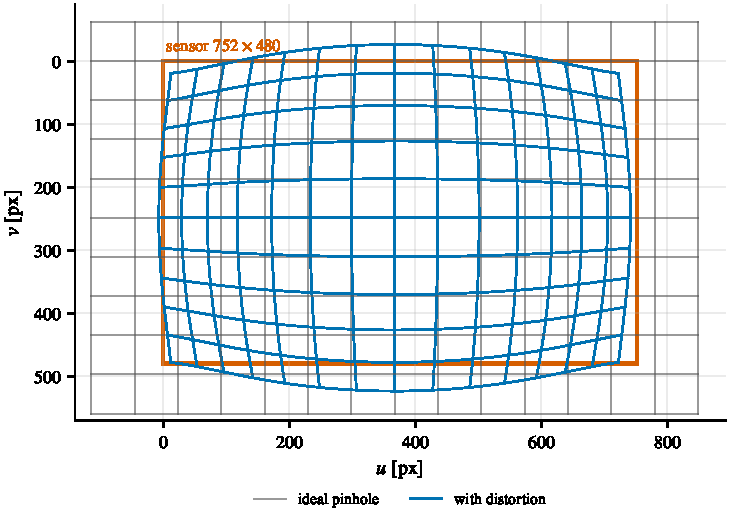
\includegraphics[width=0.84\textwidth]{fig_distortion.pdf}
  \caption{EuRoC \code{cam0} lens distortion. A regular grid in normalized coordinates (gray) is imaged by the real lens as the curved blue grid. Distortion pulls
  points toward the center, increasingly toward the edges, so the sensor (orange) sees a wider field than an ideal pinhole with the same focal length would.}
  \label{fig:distortion}
\end{figure}

\paragraph{Undistortion.} The front end measures distorted pixels and needs ideal normalized coordinates. The model has no closed-form inverse, but a fixed-point
iteration converges quickly for moderate distortion: starting from $x^{(0)} = x_d$,
\begin{equation}
  x^{(j+1)} = \frac{x_d - \Delta_x(x^{(j)}, y^{(j)})}{1 + k_1r_j^2 + k_2r_j^4},\qquad
  y^{(j+1)} = \frac{y_d - \Delta_y(x^{(j)}, y^{(j)})}{1 + k_1r_j^2 + k_2r_j^4},
\end{equation}
where $\Delta$ denotes the tangential terms. A Gauss--Newton iteration (\cref{ch:nlls}) with the $2\times2$ Jacobian of the distortion converges faster and more
reliably near the edges. OpenCV's \code{cv::undistortPoints} implements the iterative scheme. Milestone 8 checks undistortion by distorting and undistorting a
grid of points.

\begin{keyidea}[undistort points, not images]
The estimator needs a few hundred feature locations, not a rectified image. Undistorting only the tracked points costs microseconds; remapping a full image
costs milliseconds, resamples the pixels (blurring them), and changes the noise of the feature detector in a position-dependent way. Track in the raw image and
undistort the tracks.
\end{keyidea}

\paragraph{Wide-angle lenses.} Beyond about $120^\circ$ of field of view, the pinhole model itself breaks down (a ray at $90^\circ$ from the axis would have infinite
normalized coordinates). \emph{Fisheye} models parameterize the image radius as a function of the angle $\vartheta$ of the incoming ray, for example the
equidistant (Kannala--Brandt) model $r_d = \vartheta(1 + k_1\vartheta^2 + k_2\vartheta^4 + \cdots)$. The rest of the pipeline is unchanged: everything downstream of
undistortion works with bearings, which can be represented as unit vectors when they are far from the optical axis.

% ==============================================================================
\section{Camera calibration}

How were EuRoC's intrinsics and distortion coefficients obtained? By observing a known calibration target (a checkerboard or grid of markers) in many
images and fitting the camera model to the observed corner positions.

\paragraph{Zhang's method.} Place the target in the plane $Z = 0$ of its own frame. A target point $(X, Y, 0)$ then projects as
$\lambda\tilde u = K[r_1\ r_2\ r_3\ t](X, Y, 0, 1)\T = K[r_1\ r_2\ t](X, Y, 1)\T$: each image of the target is a homography $H = [h_1\ h_2\ h_3] \propto K[r_1\ r_2\ t]$, estimable from
four or more corner correspondences (\cref{ch:multiview}). Because $r_1$ and $r_2$ are orthonormal, $r_1 = \lambda K\inv h_1$ and $r_2 = \lambda K\inv h_2$ give two
constraints on the matrix $\omega = K\mT K\inv$:
\begin{equation}
  h_1\T\omega h_2 = 0, \qquad h_1\T\omega h_1 = h_2\T\omega h_2 .
\end{equation}
These are linear in the entries of the symmetric $\omega$, so three or more images determine it; $K$ follows from a Cholesky factorization of $\omega$. The linear
estimate is then refined, together with the distortion coefficients and each image's pose, by Levenberg--Marquardt (\cref{ch:nlls}) minimizing the
\emph{reprojection error}, the distance between observed and predicted corners. The residual reprojection error after calibration, typically a few tenths of a
pixel, is the standard measure of calibration quality.

\paragraph{Camera--IMU calibration.} The extrinsics $T_{bc}$ and the time offset are calibrated jointly with the IMU, by moving the rig in front of the target
(\cref{ch:imu}).

% ==============================================================================
\section{The measurement model}

\begin{convention}[camera model, AGENTS.md C6]
In normalized, undistorted image coordinates,
\begin{equation}
  p_c = R_{bc}\T\big(R_{wb}\T(p_f - p_{wb}) - p_{bc}\big), \qquad
  z = \begin{bmatrix} p_{c,x}/p_{c,z} \\ p_{c,y}/p_{c,z} \end{bmatrix} + n_{uv},
  \qquad \sigma_{uv} \approx \sigma_{px}/f .
\end{equation}
\end{convention}

The first equation chains the world-to-body and body-to-camera transformations of \eqref{eq:world-to-camera}. The noise model follows from $u = f_u x + c_u$: a pixel
error $\delta u$ corresponds to a normalized error $\delta u/f_u$. With $\sigma_{px} = 1$~px and $f \approx 458$~px, $\sigma_{uv} \approx 2.2\times10^{-3}$. Strictly, distortion makes the
mapping from pixel noise to normalized noise position-dependent, by the inverse of the distortion Jacobian, and $f_u \neq f_v$. Both effects are small for EuRoC and
conventionally ignored, but they are a legitimate refinement.

% ==============================================================================
\section{The projection Jacobian}

\begin{proposition}[Jacobian of the pinhole projection]
\label{prop:proj-jacobian}
\begin{equation}
  \frac{\partial\pi}{\partial p_c} = \frac{1}{Z}\begin{bmatrix} 1 & 0 & -X/Z \\ 0 & 1 & -Y/Z \end{bmatrix}
  = \frac1Z\begin{bmatrix} I_2 & -\pi(p_c) \end{bmatrix}.
\end{equation}
\end{proposition}
\begin{proof}
Differentiate $X/Z$ and $Y/Z$ with the quotient rule: $\partial(X/Z)/\partial X = 1/Z$, $\partial(X/Z)/\partial Z = -X/Z^2$, and similarly for $Y/Z$.
\end{proof}

The Jacobian has rank two, and its nullspace is spanned by $p_c$ itself: moving the point along its viewing ray does not change its image. This is the single-view
loss of depth in differential form, and it is why a feature must be observed from at least two sufficiently different viewpoints before it constrains anything
(\cref{ch:multiview}). The factor $1/Z$ says that distant points have small image motion for a given change in position. They constrain rotation well and
translation poorly.

The full measurement Jacobian with respect to the filter state is the chain-rule product of this matrix with the Jacobian of $p_c$ with respect to the clone pose
and the feature position. Deriving those is part of \cref{ch:msckfupdate}.

\begin{pitfall}[points behind the camera]
\eqref{eq:pinhole} happily projects points with $Z < 0$, flipping their image through the center. A triangulation or linearization that produces a negative depth must
be rejected (the \emph{cheirality} check), not projected. Points with very small positive $Z$ produce huge Jacobians and should be rejected too.
\end{pitfall}

% ==============================================================================
\section{Extrinsics and time offset}

\paragraph{Extrinsic calibration.} The transformation $T_{bc}$ between the IMU and the camera is estimated offline, for EuRoC with Kalibr~\cite{furgale2013kalibr}, and
stored as \code{T\_BS} in \code{cam0/sensor.yaml}. Its rotation is close to a permutation of axes, and its translation is a few centimeters (\cref{app:euroc}). An error of
$\delta\phi$ in the extrinsic rotation biases every predicted bearing by about $\delta\phi$, which looks to the filter like a systematic residual. A translation error matters
mostly for near points. The project treats $T_{bc}$ as exact (AGENTS.md C3). Estimating it online is a stretch goal.

\paragraph{Time offset.} If the camera timestamp differs from the IMU clock by $t_d$, a feature moving across the image at velocity $\dot z$ is measured with an error of
about $\dot z\,t_d$. A 1~ms offset at an image-plane velocity of 0.5 normalized units per second (fast rotation) is an error of $5\times10^{-4}$, a quarter of a pixel.
EuRoC is hardware synchronized, so $t_d \approx 0$; consumer devices can have offsets of tens of milliseconds and must estimate it online~\cite{li2014timeoffset}.

\begin{takeaways}
\begin{itemize}
  \item A focused lens camera has the geometry of a pinhole at the lens center; lens imperfections are modeled as distortion.
  \item Exposure time causes motion blur of about $f\omega T$ pixels; EuRoC's global shutter exposes all pixels at once.
  \item Normalized coordinates $(X/Z, Y/Z)$ are lens-independent bearings; $K$ maps them to pixels.
  \item Homogeneous coordinates make projection linear; lines through points and intersections of lines are cross products; homographies map planes and pure
        rotations between views.
  \item EuRoC's lens has strong barrel distortion; undistort the tracked points, not the images.
  \item Cameras are calibrated by fitting the model to images of a known target, minimizing reprojection error.
  \item $\partial\pi/\partial p_c = \frac1Z[I_2\ \ {-\pi(p_c)}]$; its nullspace is the viewing ray.
\end{itemize}
\end{takeaways}

\begin{exercises}
  \item A lens with $f_L = 4$~mm is focused at infinity. How far must the sensor move to focus on an object at 0.5~m?
  \item Compute the horizontal and vertical fields of view of \code{cam0} with and without distortion.
  \item Compute the intersection of the lines $x + y = 1$ and $x - y = 0$ with homogeneous coordinates, and the line through $(1, 2)$ and $(3, 1)$.
  \item Show that two parallel lines intersect at a point at infinity, and find the vanishing point of the image of a family of parallel 3D lines with
        direction $d$ under the camera $P = K[I\ \ 0]$.
  \item Implement distortion and fixed-point undistortion for the EuRoC model. How many iterations are needed for $10^{-6}$ accuracy at the image corners? Compare
        with Gauss--Newton.
  \item Derive the two linear constraints of Zhang's method from the orthonormality of $r_1$ and $r_2$.
  \item A point at depth 10~m is observed by a camera translating sideways at 1~m/s and rotating at 1~rad/s. Which motion dominates its image velocity? What does
        this imply for the observability of translation from distant points?
\end{exercises}

\chapter{Digital Image Processing}
\label{ch:imageproc}

\begin{objectives}
\begin{itemize}
  \item Treat an image as a sampled function, and filter it by convolution.
  \item Smooth images with Gaussian kernels, and understand separability and cost.
  \item Compute image gradients robustly with derivative-of-smoothing kernels such as Sobel and Scharr.
  \item Understand why images must be blurred before they are down-sampled, and build Gaussian pyramids.
  \item Interpolate images at sub-pixel positions, find local maxima, and refine them to sub-pixel accuracy.
  \item Know how photometric changes affect intensity-based methods.
\end{itemize}
\end{objectives}

Feature detection and tracking (\cref{ch:frontend}) operate on raw pixel arrays: they smooth them, differentiate them, shrink them and sample them between
pixels. This chapter develops these operations from first principles, as far as the front end needs them.

% ==============================================================================
\section{Images as functions}

A grayscale image is a function $I(u, v)$ giving the brightness at image position $(u, v)$, sampled on the integer grid of pixel centers and quantized,
typically to integers between 0 and 255. In memory it is a 2D array indexed by row and column, $I[\text{row}, \text{col}] = I(u = \text{col}, v = \text{row})$; mixing up the
two orders is a classic bug. Color images have three such channels; a monochrome image can be formed as a weighted sum of them. EuRoC's cameras are
monochrome.

Between pixels, $I$ is undefined until we decide how to interpolate it (\cref{sec:interpolation}). Its derivatives must be approximated by differences of
nearby pixels (\cref{sec:image-derivatives}). Both operations are sensitive to noise and to aliasing, which is what the rest of this chapter is about.

% ==============================================================================
\section{Linear filtering}

\subsection{Correlation and convolution}

\index{convolution}
\termi{Linear filtering}{linear filtering} replaces each pixel by a weighted sum of its neighbors, with the weights given by a small array $h$, the \emph{kernel}. Two closely related
forms exist:
\begin{equation}
\begin{aligned}
  \text{correlation:}&\quad (h\star I)[u, v] = \sum_{i,j}h[i, j]\,I[u + i, v + j], \\
  \text{convolution:}&\quad (h * I)[u, v] = \sum_{i,j}h[i, j]\,I[u - i, v - j] .
\end{aligned}
\end{equation}
Convolution flips the kernel; for symmetric kernels the two coincide. Both are \emph{linear} and \emph{shift-invariant}: filtering a shifted image gives the shifted
filtered image. Convolution is also commutative and associative, so a cascade of filters equals a single filter, $h_2 * (h_1 * I) = (h_2 * h_1) * I$. Near the image
border the kernel extends past the edge, and the missing pixels must be invented: by zeros, by replicating the border, or by reflecting the image. Results
within a kernel radius of the border are always less reliable, which is why detectors ignore a margin there.

A $k\times k$ kernel costs $k^2$ multiplications per pixel. A kernel that factors as an outer product of a column and a row, $h = h_vh_u\T$, is \emph{separable}: filtering
with $h$ equals filtering the rows with $h_u$ and then the columns with $h_v$, at a cost of $2k$ per pixel.

\subsection{Smoothing}

Averaging neighbors reduces noise. The simplest kernel, the \emph{box filter}, averages a $k\times k$ square. The \term{Gaussian filter} weights neighbors by
\begin{equation}
  G_\sigma(u, v) = \frac{1}{2\pi\sigma^2}\exp\!\Big(-\frac{u^2 + v^2}{2\sigma^2}\Big) = g_\sigma(u)\,g_\sigma(v), \qquad g_\sigma(x) = \frac{1}{\sqrt{2\pi}\sigma}e^{-x^2/2\sigma^2},
\end{equation}
sampled at integer offsets, truncated at about $\pm3\sigma$ and renormalized to sum to one. The factorization shows that it is separable. The Gaussian is preferred
over the box because it has no sharp edges: its frequency response is itself a Gaussian, which removes high frequencies smoothly without the ripples of the
box filter. Cascading two Gaussian filters gives a Gaussian whose variances add, $G_{\sigma_1}*G_{\sigma_2} = G_{\sqrt{\sigma_1^2 + \sigma_2^2}}$. Small Gaussians are well
approximated by binomial kernels, $\tfrac14[1, 2, 1]$ and $\tfrac1{16}[1, 4, 6, 4, 1]$ in each direction.

% ==============================================================================
\section{Image derivatives}
\label{sec:image-derivatives}

\index{image gradient}
The \term{image gradient} $\nabla I = (I_u, I_v)$ points in the direction of fastest brightness increase, and its magnitude measures the local contrast. It is
approximated by differences, for example the central difference $I_u[u, v] \approx \tfrac12(I[u + 1, v] - I[u - 1, v])$, a correlation with $\tfrac12[-1, 0, 1]$.

Differentiation amplifies noise: a derivative multiplies each frequency component by its frequency, so pixel-to-pixel noise, the highest frequency present,
is amplified most. The remedy is to smooth before differentiating, and since both are convolutions, to combine them into one kernel. The \emph{Sobel}
operator smooths across the derivative direction with $[1, 2, 1]$ and differentiates along it:
\begin{equation}
  S_u = \begin{bmatrix} 1 \\ 2 \\ 1 \end{bmatrix}\begin{bmatrix} -1 & 0 & 1 \end{bmatrix} = \begin{bmatrix} -1 & 0 & 1 \\ -2 & 0 & 2 \\ -1 & 0 & 1 \end{bmatrix},
  \qquad S_v = S_u\T .
\end{equation}
The \emph{Scharr} operator uses $[3, 10, 3]$ instead of $[1, 2, 1]$, which gives gradient directions that are more accurate for all orientations; OpenCV's
Lucas--Kanade tracker uses it. More generally, the \emph{derivative of a Gaussian}, $\partial G_\sigma/\partial u$, smooths and differentiates at a chosen scale $\sigma$.
Whatever the kernel, it is a weighted difference: its entries sum to zero, so it ignores uniform brightness, and its scale must be divided out when absolute
gradient values matter (Sobel's sum of positive weights is 4 times the step, so $S_u\star I \approx 8I_u$).

\begin{figure}[t]
  \centering
  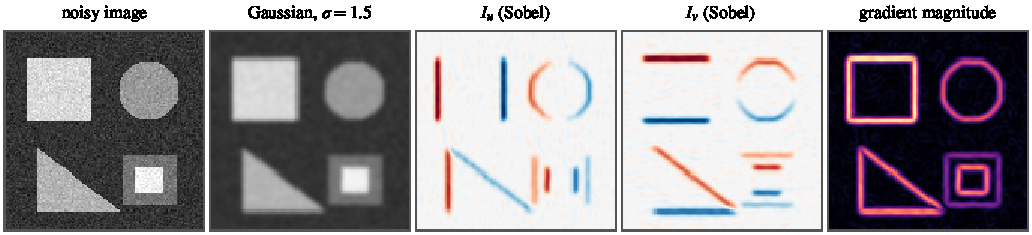
\includegraphics[width=\textwidth]{fig_image_filters.pdf}
  \caption{A synthetic noisy image, its Gaussian smoothing ($\sigma = 1.5$~px), its Sobel derivatives $I_u$ and $I_v$, and the gradient magnitude. Vertical edges respond in
  $I_u$, horizontal edges in $I_v$; corners respond in both, which is what corner detectors look for.}
  \label{fig:image-filters}
\end{figure}

% ==============================================================================
\section{Sampling, aliasing and pyramids}
\label{sec:pyramids}

\subsection{Aliasing in images}

An image is a sampled signal, and the sampling theorem (\cref{ch:processes}) applies in each direction: a pixel grid can represent spatial frequencies up to half a
cycle per pixel. Shrinking an image by keeping every other pixel halves the representable frequency. Any finer detail does not vanish: it \emph{aliases} into false
coarse patterns (moir\'e). The cure is the same as for any sampled signal: low-pass filter, by blurring, before down-sampling.

\begin{figure}[t]
  \centering
  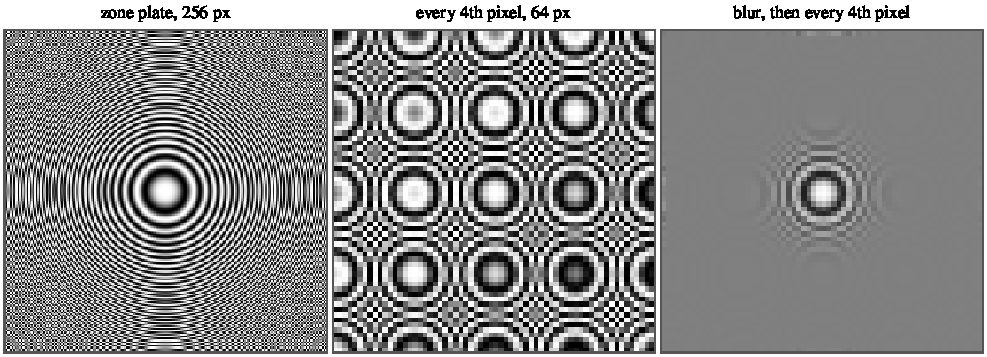
\includegraphics[width=\textwidth]{fig_aliasing_image.pdf}
  \caption{Aliasing in images. A ``zone plate'', whose spatial frequency increases away from the center (left), is shrunk four times by keeping every fourth pixel
  (middle) and by Gaussian blurring first (right). Naive sub-sampling creates false ring patterns; blurring removes the frequencies that cannot be represented.}
  \label{fig:aliasing-image}
\end{figure}

\subsection{Gaussian pyramids}

\index{image pyramid}
A \term{Gaussian pyramid} is a sequence of images, each a blurred and half-resolution copy of the previous one:
\begin{equation}
  I_{\ell+1} = \downarrow_2\big(G * I_\ell\big),
\end{equation}
where $G$ is a small Gaussian (OpenCV's \code{pyrDown} uses the binomial kernel $\tfrac1{16}[1, 4, 6, 4, 1]$ in each direction) and $\downarrow_2$ keeps every second row and
column. Level $\ell$ has $2^{-\ell}$ of the original resolution in each direction, so a pixel position $u_0$ at level 0 corresponds to $u_\ell \approx u_0/2^\ell$ at level $\ell$ (up
to half-pixel conventions). The whole pyramid costs only a third more memory than the original image ($1 + \tfrac14 + \tfrac1{16} + \cdots = \tfrac43$).

\begin{figure}[t]
  \centering
  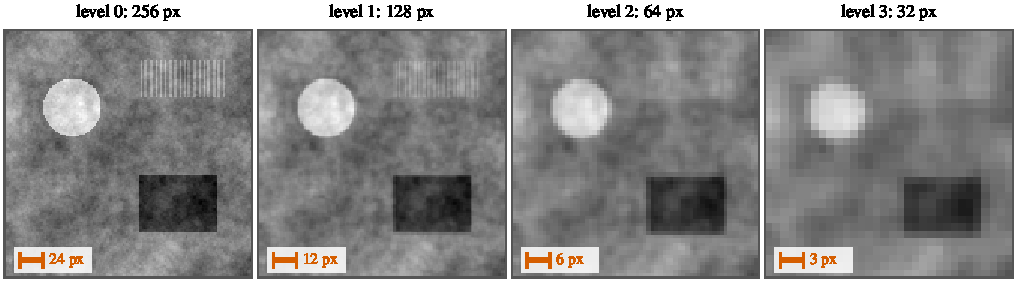
\includegraphics[width=\textwidth]{fig_pyramid.pdf}
  \caption{Four levels of a Gaussian pyramid of a textured synthetic image, displayed at a common size. Fine texture disappears level by level; coarse structure
  survives. A displacement of 24~px at level 0 is a displacement of 3~px at level 3.}
  \label{fig:pyramid-levels}
\end{figure}

Pyramids serve two purposes in the front end. Motion that is large in pixels at full resolution is small at coarse levels, where an iterative tracker can
capture it (\cref{ch:frontend}). And structures of different sizes are best detected at different scales.

% ==============================================================================
\section{Interpolation}
\label{sec:interpolation}

\index{bilinear interpolation}
Sub-pixel tracking needs image values and gradients at non-integer positions. Writing a position as $(u_0 + a, v_0 + b)$ with integer $(u_0, v_0)$ and fractional parts
$a, b \in [0, 1)$:
\begin{itemize}
  \item \emph{nearest neighbor} takes the closest pixel: fast, but the result jumps as the position moves, which ruins sub-pixel accuracy;
  \item \term{bilinear interpolation} interpolates linearly in $u$ along the two neighboring rows and then linearly in $v$ between the results:
  \begin{equation}
    I(u_0 + a, v_0 + b) = (1 - a)(1 - b)\,I_{00} + a(1 - b)\,I_{10} + (1 - a)b\,I_{01} + ab\,I_{11},
  \end{equation}
  with $I_{ij} = I[u_0 + i, v_0 + j]$. The result is continuous, and the weights are the areas of the rectangles opposite each corner;
  \item \emph{bicubic} interpolation fits a smooth cubic patch to a $4\times4$ neighborhood; it has continuous derivatives at the cost of 16 pixels per sample.
\end{itemize}
Lucas--Kanade trackers use bilinear interpolation for both the image and its gradients. With images represented as 8-bit integers, implementations use fixed-point
weights for speed, which limits the attainable sub-pixel resolution to a few hundredths of a pixel, well below the noise of real tracking.

% ==============================================================================
\section{Finding local maxima}

Detectors compute a response map (corner strength, for example) and select the pixels where it is large \emph{and} locally maximal. \termi{Non-maximum suppression}{non-maximum suppression}
keeps a pixel only if its response exceeds a threshold and is the largest in its neighborhood (a $3\times3$ window, or a larger radius to enforce spacing between
detections). The location of a maximum can then be refined below the pixel grid by fitting a parabola through the response $r_{-1}, r_0, r_1$ at the maximum and its two
neighbors in each direction; the vertex lies at the offset
\begin{equation}
  \delta = \frac{r_{-1} - r_{1}}{2\,(r_{-1} - 2r_0 + r_{1})}
\end{equation}
pixels from the center. Sub-pixel accuracy at the detection stage is less important for tracking-based front ends, whose tracker refines positions anyway.

% ==============================================================================
\section{Photometric changes}

Intensity-based methods assume that a scene point keeps its brightness between frames (\cref{ch:frontend}). Auto-exposure, lighting changes and non-Lambertian
surfaces violate this. A common model is an affine change, $I_2 \approx \alpha I_1 + \beta$. Gradients are unaffected by $\beta$, and comparing patches after subtracting their
means and dividing by their standard deviations (\emph{zero-mean normalized cross-correlation}) is unaffected by both. Some trackers estimate $\alpha$ and $\beta$
along with the motion; others pre-process images, for example with histogram equalization, to reduce the variation.

\begin{takeaways}
\begin{itemize}
  \item Filtering is convolution with a kernel; separable kernels cost $2k$ instead of $k^2$ per pixel.
  \item Gaussian smoothing reduces noise without ringing; variances of cascaded Gaussians add.
  \item Derivatives amplify noise; Sobel, Scharr and derivative-of-Gaussian kernels smooth and differentiate at once.
  \item Down-sampling without blurring aliases; a Gaussian pyramid blurs and halves the resolution at each level.
  \item Bilinear interpolation gives continuous sub-pixel samples; non-maximum suppression and parabola fits localize detections.
  \item Normalize patches when brightness may change between frames.
\end{itemize}
\end{takeaways}

\begin{exercises}
  \item Show that the 2D Gaussian kernel is separable, and that filtering with it costs $2k$ operations per pixel for a $k$-tap kernel.
  \item Show that convolving $\tfrac12[1, 1]$ with itself repeatedly produces the binomial kernels, and that their variance grows linearly with the number of
        convolutions.
  \item Compute the response of the Sobel kernel $S_u$ to a linear ramp $I(u, v) = cu$, and explain the factor 8.
  \item Generate a zone plate and reproduce \cref{fig:aliasing-image}. How large must the blur be before shrinking by 4?
  \item Derive the bilinear interpolation formula by interpolating first along $u$ and then along $v$, and show that the result does not depend on the order.
  \item Derive the parabola-vertex formula for sub-pixel peak refinement.
\end{exercises}
% Solutions to the exercises of Chapter 21.
\begin{solutions}
  \item The exponent splits, $e^{-(u^2 + v^2)/2\sigma^2} = e^{-u^2/2\sigma^2}e^{-v^2/2\sigma^2}$, and so does the constant, $\frac1{2\pi\sigma^2} = \frac1{\sqrt{2\pi}\sigma}\cdot\frac1{\sqrt{2\pi}\sigma}$, so
        $G_\sigma(u, v) = g_\sigma(u)g_\sigma(v)$. Sampled on a square $k\times k$ grid the kernel is the outer product $h = gg\T$ of the sampled 1D kernel, and normalizing
        each 1D kernel to unit sum normalizes the product too. Then
        \[
          (h * I)[u, v] = \sum_jg[j]\Big(\sum_ig[i]\,I[u - i, v - j]\Big):
        \]
        the inner sum filters every row with $g$ ($k$ multiplications per pixel) and the outer sum filters the columns of the result ($k$ more), $2k$ in total
        instead of $k^2$. For $\sigma = 1.5$ truncated at $\pm3\sigma$ ($k = 11$) this is 22 instead of 121. Truncating to a \emph{disk} instead of a square would destroy
        the factorization.

  \item The kernel $[a_0, \dots, a_n]$ corresponds to the polynomial $\sum_ia_iz^i$, and convolution of kernels is multiplication of polynomials. Convolving
        $\tfrac12[1, 1]$ with itself $n$ times gives $\big(\tfrac12(1 + z)\big)^n = 2^{-n}\sum_i\binom{n}{i}z^i$: the binomial kernels $\tfrac14[1, 2, 1]$, $\tfrac18[1, 3, 3, 1]$, $\tfrac1{16}[1, 4, 6, 4, 1]$, \dots.
        A non-negative kernel with unit sum is a probability distribution, and the convolution of two distributions is the distribution of the sum of
        independent variables, whose variances add (\cref{ch:prob}). The two-point kernel $\tfrac12[1, 1]$ has variance $\tfrac14$, so the $n$-fold kernel has variance $n/4$:
        $\tfrac12$ for $[1, 2, 1]$, $1$ for $[1, 4, 6, 4, 1]$. By the central limit theorem the binomial kernels approach Gaussians with $\sigma = \sqrt n/2$; OpenCV's
        \code{pyrDown} kernel is a Gaussian with $\sigma = 1$~px.

  \item At pixel $(u, v)$ the correlation sums $S_u[j, i]\,c\,(u + i)$. In each row the weights $-1, 0, 1$ give $c(u + 1) - c(u - 1) = 2c$, and the three rows are
        weighted $1, 2, 1$, so
        \[
          (S_u\star I)[u, v] = (1 + 2 + 1)\cdot2c = 8c,
        \]
        everywhere, for a true derivative $I_u = c$. The factor 8 is the product of the smoothing kernel's sum (4) and the distance between the differenced
        pixels (2). Divide by 8 to obtain the gradient (by 32 for Scharr, whose smoothing kernel sums to 16). With convolution instead of correlation the
        kernel is flipped and the response is $-8c$: check the sign convention of whatever library you use.

  \item A zone plate $I = \tfrac12 + \tfrac12\cos(\pi r^2/n)$ on an $n\times n$ grid (the figure uses $n = 256$) has phase $\pi r^2/n$, hence local frequency $r/n$ cycles per pixel. After
        keeping every fourth pixel the representable limit is $\tfrac18$ cycle per original pixel, so the true rings beyond $r = n/8 = 32$ cannot be represented
        and should become uniform gray; instead, naive sub-sampling folds them into false rings, with new ``centers'' where the frequency is a multiple of the
        new sampling rate $\tfrac14$. A Gaussian blur multiplies frequency $f$ by $e^{-2\pi^2\sigma^2f^2}$. Measuring the false pattern in the region $48 < r < 128$:
        \begin{center}\small
        \begin{tabular}{@{}l c c c c c@{}}
        \toprule
        blur $\sigma$ (px) & 0 & 1 & 1.5 & 2 & 3 \\
        \midrule
        RMS of false pattern & 0.353 & 0.061 & 0.018 & 0.005 & 0.002 \\
        response at $f = \tfrac18$ (kept detail) & 1 & 0.73 & 0.50 & 0.29 & 0.06 \\
        response at $f = \tfrac14$ (aliases to DC) & 1 & 0.29 & 0.06 & 0.007 & $10^{-5}$ \\
        \bottomrule
        \end{tabular}
        \end{center}
        A blur of $\sigma \approx 2$~px, half the shrink factor, removes the aliasing (as in \cref{fig:aliasing-image}); much more also removes detail the smaller image could
        have kept. The same rule, $\sigma \approx s/2$ for a shrink by $s$, gives \code{pyrDown}'s $\sigma = 1$ for $s = 2$.

  \item Along the row $v_0$, linear interpolation gives $(1 - a)I_{00} + aI_{10}$, and along the row $v_0 + 1$, $(1 - a)I_{01} + aI_{11}$. Interpolating these linearly in $v$ with
        weights $1 - b$ and $b$ gives the formula of \cref{sec:interpolation}. In the other order, the columns give $(1 - b)I_{00} + bI_{01}$ and $(1 - b)I_{10} + bI_{11}$, and
        interpolating in $u$ gives $(1 - a)(1 - b)I_{00} + (1 - a)bI_{01} + a(1 - b)I_{10} + abI_{11}$, the same four products. Without expanding: both results have the form
        $c_0 + c_1a + c_2b + c_3ab$ and take the four corner values at the corners, and those four conditions determine the four coefficients uniquely. The
        interpolant is linear along every row and column but quadratic along diagonals, and its derivatives jump at pixel boundaries.

  \item Fit $r(x) = Ax^2 + Bx + C$ through $(-1, r_{-1})$, $(0, r_0)$, $(1, r_1)$: $C = r_0$, $A + B + C = r_1$ and $A - B + C = r_{-1}$, so
        $B = \tfrac12(r_1 - r_{-1})$ and $A = \tfrac12(r_{-1} - 2r_0 + r_1)$. The vertex is at
        \[
          \delta = -\frac{B}{2A} = \frac{r_{-1} - r_1}{2(r_{-1} - 2r_0 + r_1)} .
        \]
        If $r_0$ is the largest of the three, $A < 0$ (a maximum), and $|r_{-1} - r_1| \le (r_0 - r_{-1}) + (r_0 - r_1) = 2|A|$, so $|\delta| \le \tfrac12$: the refined peak stays within
        the pixel. Real peaks are not parabolas, and the fit is biased toward the pixel center: for a Gaussian peak of width $\sigma = 1$~px at a true
        offset of $0.3$~px it returns $0.25$, a bias of up to $0.05$~px, larger for sharper peaks.
\end{solutions}


\chapter{Feature Detection and Tracking}
\label{ch:frontend}

\begin{objectives}
\begin{itemize}
  \item Derive the structure tensor from the auto-correlation of an image patch, and understand corner detectors (Harris, Shi--Tomasi, FAST).
  \item Derive Lucas--Kanade optical flow from brightness constancy, as a Gauss--Newton problem, including the aperture problem.
  \item Implement iterative, pyramidal Lucas--Kanade tracking, and know its failure modes.
  \item Build a robust tracking pipeline: bucketing, forward-backward checks, IMU-aided prediction and geometric verification.
  \item Manage feature tracks through their life cycle with bounded memory.
\end{itemize}
\end{objectives}

The front end turns a stream of images into \emph{feature tracks}: for each tracked scene point, the list of its undistorted normalized coordinates in the images
where it was seen, with the image timestamps. Everything the MSCKF knows about the scene comes from these tracks, so their quality bounds the quality of the
estimator.

\begin{figure}[h]
\centering
\begin{tikzpicture}[node distance=4mm and 5mm, every node/.style={block, font=\footnotesize, minimum width=19mm}]
  \node (img) {image $k$};
  \node (pyr) [right=of img] {build\\pyramid};
  \node (lk) [right=of pyr] {track with\\pyramidal LK};
  \node (fb) [right=of lk] {forward-\\backward check};
  \node (und) [below=of fb] {undistort\\points};
  \node (ran) [left=of und] {RANSAC\\(E or 2-pt)};
  \node (det) [left=of ran] {detect new\\corners (grid)};
  \node (out) [left=of det, fill=white] {tracks to\\estimator};
  \draw[->] (img) -- (pyr); \draw[->] (pyr) -- (lk); \draw[->] (lk) -- (fb);
  \draw[->] (fb) -- (und); \draw[->] (und) -- (ran); \draw[->] (ran) -- (det); \draw[->] (det) -- (out);
\end{tikzpicture}
\caption{A KLT-based front end, as used by MSCKF-style estimators.}
\label{fig:frontend-pipeline}
\end{figure}

% ==============================================================================
\section{What makes a good feature}

\subsection{The auto-correlation of a patch}

A feature is useful if it can be found again, precisely, in the next image. Consider a small window $W$ around a point and ask how much the window changes when
shifted by a small displacement $d$. Measure the change by the weighted sum of squared differences
\begin{equation}
  E(d) = \sum_{x\in W}w(x)\,\big(I(x + d) - I(x)\big)^2,
\end{equation}
with a window function $w$ (uniform, or a Gaussian that emphasizes the center). By a first-order Taylor expansion $I(x + d) \approx I(x) + \nabla I(x)\T d$, so
\begin{equation}
  E(d) \approx \sum_{x\in W}w(x)\,\big(\nabla I(x)\T d\big)^2 = d\T M\,d,
  \qquad
  M = \sum_{x\in W}w(x)\begin{bmatrix} I_u^2 & I_uI_v \\ I_uI_v & I_v^2 \end{bmatrix},
  \label{eq:structure-tensor}
\end{equation}
with the gradients $I_u$, $I_v$ computed as in \cref{sec:image-derivatives}. $M$ is the \term{structure tensor} (second-moment matrix) of the window: a symmetric PSD
$2\times2$ matrix, so $E(d)$ is a quadratic form whose level sets are ellipses (\cref{fig:ellipse}). Its eigenvalues $\lambda_1 \ge \lambda_2 \ge 0$ describe how distinctive the
window is.
\begin{itemize}
  \item Both small: the window is \emph{flat}; it looks the same after any small shift.
  \item One large, one small: an \emph{edge}; shifting along the edge (the eigenvector of $\lambda_2$) changes nothing.
  \item Both large: a \emph{corner}; every shift changes the window, so its position is well defined in two dimensions.
\end{itemize}
By the Rayleigh quotient (\cref{prop:rayleigh}), $\lambda_2$ is the smallest change $E(d)$ caused by any unit shift: the worst-case distinctiveness.

\subsection{Corner detectors}

\index{Harris detector}\index{Shi--Tomasi detector}
The \term{Harris detector}~\cite{harris1988corner} scores each pixel with $\det M - k(\tr M)^2 = \lambda_1\lambda_2 - k(\lambda_1 + \lambda_2)^2$, with $k \approx 0.04$--$0.06$, which avoids computing
eigenvalues. The \term{Shi--Tomasi detector}~\cite{shi1994good} scores $\lambda_2 = \min(\lambda_1, \lambda_2)$ directly (\cref{fig:structure-tensor}), computed in closed form for a $2\times2$
matrix as $\tfrac12\big(\tr M - \sqrt{(\tr M)^2 - 4\det M}\big)$. Both are followed by thresholding and non-maximum suppression. Shi--Tomasi has a deeper justification: it
selects exactly the windows for which the tracker of the next section is well conditioned.

\begin{figure}[t]
  \centering
  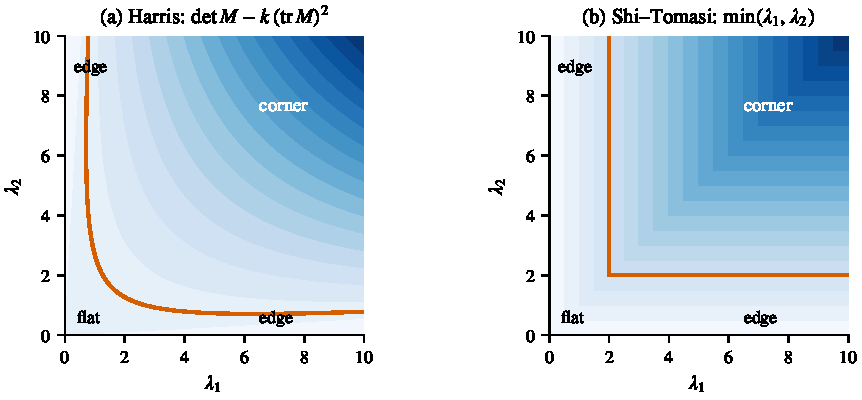
\includegraphics[width=\textwidth]{fig_structure_tensor.pdf}
  \caption{Corner scores over the plane of structure-tensor eigenvalues, with a threshold contour (orange). Both scores accept only windows with two large
  eigenvalues. Shi--Tomasi's $\min(\lambda_1, \lambda_2)$ is exactly the quantity that makes the Lucas--Kanade system well conditioned.}
  \label{fig:structure-tensor}
\end{figure}

\begin{figure}[t]
  \centering
  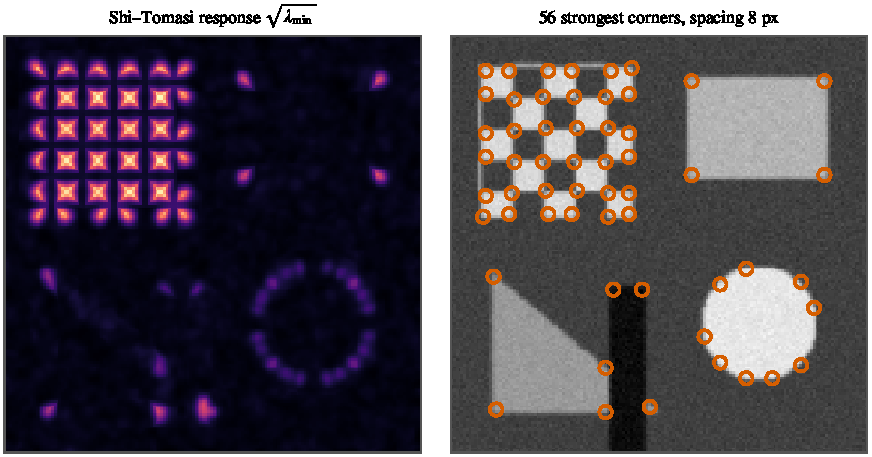
\includegraphics[width=\textwidth]{fig_harris.pdf}
  \caption{Shi--Tomasi corner response on a synthetic image (left), and the strongest corners after non-maximum suppression with a minimum spacing of 8~px (right).
  Edges and flat regions get low scores; corners and blob-like texture get high ones.}
  \label{fig:harris}
\end{figure}

Other detectors trade quality for speed. FAST classifies a pixel as a corner if a long enough arc of the 16 pixels on a circle around it is uniformly brighter or
darker than the center, using only comparisons; it is very fast but noisier. Detectors used for matching across large viewpoint changes add \emph{scale}
selection (detecting at several pyramid levels) and an \emph{orientation} for each feature, as ORB does. A frame-to-frame tracker needs neither.

% ==============================================================================
\section{Lucas--Kanade optical flow}

\subsection{Brightness constancy and the aperture problem}

Assume that a scene point keeps its brightness between consecutive frames, $I_{k+1}(x + d) = I_k(x)$, where $d$ is the image motion of the point. Linearizing in $d$,
\begin{equation}
  I_{k+1}(x) + \nabla I\T d \approx I_k(x)
  \quad\Longleftrightarrow\quad
  I_u\,d_u + I_v\,d_v + I_t = 0, \qquad I_t = I_{k+1}(x) - I_k(x).
  \label{eq:ofc}
\end{equation}
This \emph{optical-flow constraint} is one equation in two unknowns. It determines only the component of $d$ along the gradient: motion along an edge is invisible.
This is the \term{aperture problem}, the same phenomenon seen through a small hole when a long line slides past: only its perpendicular motion is visible.

\subsection{The Lucas--Kanade solution}

\index{Lucas--Kanade tracker}
Lucas and Kanade~\cite{lucas1981iterative} assume the displacement is the same for all pixels of a small window, which provides many equations for the two
unknowns, and solve \eqref{eq:ofc} for all of them in the least-squares sense:
\begin{equation}
  \min_d \sum_{x\in W}w(x)\big(\nabla I(x)\T d + I_t(x)\big)^2
  \quad\Longrightarrow\quad
  M\,d = -\sum_{x\in W}w(x)\,I_t(x)\,\nabla I(x),
  \label{eq:lk}
\end{equation}
with the structure tensor $M$ of \eqref{eq:structure-tensor} as the normal matrix (\cref{sec:least-squares}). The system is solvable and well conditioned exactly when both
eigenvalues of $M$ are large compared with the image noise: Shi and Tomasi's insight was to select features by the very criterion that makes them trackable. With
image noise of variance $\sigma_I^2$ per pixel, the covariance of the estimated displacement is approximately $\sigma_I^2M\inv$ (\cref{prop:wls-cov}), so $1/\sqrt{\lambda_2}$ measures
how precisely the worst direction is tracked.

\subsection{Iterative refinement}

\Cref{eq:lk} rests on a linearization that holds only for small $d$. The full problem, minimizing $\sum_xw(x)(I_{k+1}(x + d) - I_k(x))^2$ over $d$, is a nonlinear least-squares
problem, and Lucas--Kanade is its Gauss--Newton solution (\cref{ch:nlls}):

\begin{algorithm}[h]
\caption{Iterative Lucas--Kanade for one feature}
\label{alg:lk}
\begin{algorithmic}[1]
\Require images $I_k$, $I_{k+1}$; feature position $x_0$; initial guess $d$ (zero, or a prediction)
\State compute the template $T(x) = I_k(x)$ and its gradients over the window around $x_0$; compute $M$ and factor it
\Repeat
  \State sample $I_{k+1}(x + d)$ over the window with bilinear interpolation (\cref{sec:interpolation})
  \State $e(x) \gets I_{k+1}(x + d) - T(x)$ \Comment{residual image}
  \State solve $M\,\Delta d = -\sum_xw(x)\,e(x)\,\nabla T(x)$
  \State $d \gets d + \Delta d$
\Until{$\|\Delta d\| < 0.01$~px or the iteration limit is reached}
\end{algorithmic}
\end{algorithm}

Using the gradients of the \emph{template} $T = I_k$ rather than of the warped image lets $M$ be computed and factored once per feature (the \emph{inverse
compositional} idea, analyzed by Baker and Matthews~\cite{baker2004lk}). Sub-pixel accuracy comes from the bilinear interpolation. A few iterations usually
suffice when the initial guess is within the window radius.

\subsection{Pyramids}

The linearization is valid only for displacements smaller than the scale over which the image gradient is roughly constant, about the window radius. Fast motion
violates this: at 1~rad/s and 20~Hz, the image moves by about 23~px between frames. The remedy is a Gaussian pyramid (\cref{sec:pyramids}). Tracking starts at the
coarsest level, where a 24-pixel motion becomes a 3-pixel motion; the result, doubled, initializes the next finer level, and so on down to full resolution
(\cref{fig:pyramid})~\cite{bouguet2001pyramidal}. With $L$ levels above the base, the trackable displacement grows by about $2^L$.

\begin{figure}[t]
\centering
\begin{tikzpicture}[scale=0.9]
  \foreach \l/\s/\y in {0/3.2/0, 1/1.6/2.0, 2/0.8/3.2, 3/0.4/3.95} {
    \draw[fill=primarylight, draw=primary] (-\s, \y) -- (\s, \y) -- ({\s*0.75}, {\y + 0.35}) -- ({-\s*0.75}, {\y + 0.35}) -- cycle;
    \node[font=\footnotesize, right] at ({\s + 0.2}, {\y + 0.15}) {level \l: $\frac{1}{2^{\l}}$ resolution};
  }
  \draw[->, plotorange, thick] (-0.3,4.2) -- (-0.15,3.55) -- (0.2,2.4) -- (0.9,0.25);
  \node[plotorange, font=\footnotesize, align=right, left] at (-2.0,3.2) {coarse estimate,\\refined at each level};
\end{tikzpicture}
\caption{Pyramidal tracking. A displacement that is too large to linearize at full resolution is small at the top level; each level doubles the estimate and refines
it.}
\label{fig:pyramid}
\end{figure}

\begin{figure}[t]
  \centering
  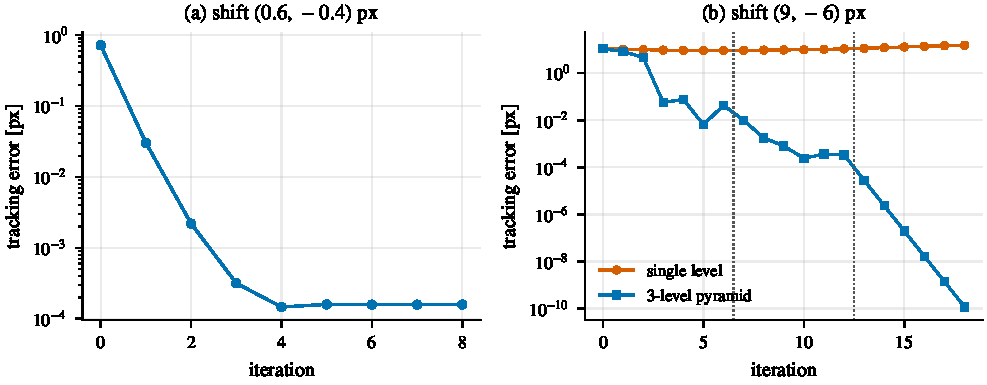
\includegraphics[width=\textwidth]{fig_lk.pdf}
  \caption{Lucas--Kanade on a synthetic textured image. (a) For a small shift of $(0.6, -0.4)$~px, the tracking error falls by orders of magnitude in a few
  Gauss--Newton iterations. (b) For a shift of $(9, -6)$~px, single-level tracking stalls in a wrong local minimum, while a three-level pyramid converges.}
  \label{fig:lk}
\end{figure}

\subsection{When tracking fails}

Lucas--Kanade fails when its assumptions fail: on edges and flat regions (an ill-conditioned $M$, the aperture problem); under occlusion, when the point disappears
behind another object; under strong brightness changes (\cref{ch:imageproc}); under motion blur, which smears the texture the tracker relies on; and when the
window straddles a depth discontinuity, where the two halves move differently. Most failures go undetected by the tracker itself, which returns a confident but wrong
position. Hence the checks of the next section.

% ==============================================================================
\section{Making tracking robust}

Optical flow optimizes photometric similarity, not physical correctness. It will track the shadow of a moving object, a specular highlight, or a T-junction formed by
two objects at different depths. Several layers of checks remove such tracks.
\begin{enumerate}
  \item \textbf{Forward-backward consistency.} Track each point from frame $k$ to $k+1$, then back to $k$. A correct track returns to its starting point; reject it if
        the round-trip error exceeds a fraction of a pixel.
  \item \textbf{IMU-aided prediction.} The gyroscope predicts the rotation between frames, $R_{c_2c_1} = R_{bc}\T R_{b_1b_2}\T R_{bc}$, where $R_{b_1b_2}$ is the integrated gyro rotation.
        For distant points, or a purely rotating camera, image points move by the infinite homography (\cref{ch:camera}): in pixels,
        $\tilde u_2 \propto KR_{c_2c_1}K\inv\tilde u_1$ (after undistortion). Starting LK from this prediction gives it a much better initial guess, and allows smaller windows and
        fewer pyramid levels.
  \item \textbf{Geometric verification.} Reject tracks that violate the epipolar constraint, with essential-matrix or two-point RANSAC, or the rotation-only constraint under
        low parallax (\cref{ch:multiview}).
  \item \textbf{Statistical gating in the filter.} Tracks that pass all of the above are still gated by the $\chi^2$ test of the MSCKF update (\cref{ch:msckfupdate}).
\end{enumerate}

\subsection{Feature distribution}

Asking a detector for the 200 strongest corners typically returns clusters on the most textured object in view. Clustered features constrain the motion poorly:
features in a small patch of the image make rotation and translation hard to separate. The standard remedy is \emph{grid bucketing}: divide the image into cells
(for example $8\times6$) and cap the number of features per cell, plus a minimum distance between features. New features are detected only in cells that have fallen
below their quota, using a mask around existing tracks. A uniform distribution of bearings makes the stacked measurement Jacobian better conditioned, which is
exactly what the estimator needs.

% ==============================================================================
\section{The feature life cycle}

\begin{figure}[h]
\centering
\begin{tikzpicture}[node distance=13mm and 34mm, every node/.style={font=\small}]
  \node[block] (new) {NEW};
  \node[block, right=of new] (trk) {TRACKED};
  \node[block, right=of trk] (lost) {LOST};
  \node[block, below=of trk, fill=white] (used) {consumed by update\\or discarded};
  \draw[->, thick] (new) -- node[above, font=\footnotesize]{tracked} (trk);
  \draw[->, thick] (trk) edge[loop above] node[above, font=\footnotesize]{tracked again} (trk);
  \draw[->, thick] (trk) -- node[above, font=\footnotesize]{track fails} (lost);
  \draw[->, thick] (lost) |- (used);
  \draw[->, thick] (trk) -- node[right, font=\footnotesize, align=left]{oldest observation's\\clone leaving the window} (used);
  \draw[->, thick] (new) |- node[left, font=\footnotesize, pos=0.25]{rejected} (used);
\end{tikzpicture}
\caption{Feature life cycle. A track is handed to the MSCKF update when it is lost, or when its oldest observation is about to leave the sliding window
(AGENTS.md F5). Its observations are used once and then discarded.}
\label{fig:lifecycle}
\end{figure}

Each feature has a persistent ID and a history of observations: (clone index or image timestamp, normalized coordinates). Since the estimator can only use
observations made at times that still have a clone in the window, the history never needs to exceed \code{kMaxClones} entries. That makes it possible to store all
tracks in a fixed-capacity pool with fixed-capacity histories, so the steady state of the front end performs no allocation for its bookkeeping (Milestone 9).

\begin{pitfall}[using a measurement twice]
Once a track's observations have been used in an MSCKF update, they must never be used again, not even partially. Re-using them double counts the same information
and makes the filter overconfident. If a track continues after being used (because its oldest clone was marginalized), its subsequent observations start a fresh
track.
\end{pitfall}

% ==============================================================================
\section{Engineering the front end}

The front end is the one component allowed to allocate (AGENTS.md E4), because OpenCV allocates internally, but it must reuse its buffers. In practice: keep the
previous pyramid and swap it with the new one instead of rebuilding storage; preallocate point vectors with \code{reserve}; keep the \code{cv::Mat} objects as members
so that their memory is reused when sizes do not change; and \emph{measure} the remaining allocations with the allocation guard rather than claiming they are zero.
Feature tracking is typically the most expensive part of the pipeline in time, too, so bucketing parameters, window size and pyramid depth are the main
performance knobs.

Descriptor-based front ends (ORB, BRIEF) describe each feature by a binary string of intensity comparisons in its neighborhood and match features across frames by
the Hamming distance between descriptors, rejecting ambiguous matches whose best and second-best distances are similar (the \emph{ratio test}). They handle large
viewpoint changes and re-detection after occlusion, which matters for loop closure, but for frame-to-frame VIO at 20~Hz KLT tracking is cheaper and more accurate.
Direct methods skip features altogether and use photometric error in the estimator itself.

\begin{projectlink}[Milestones 8 and 9]
M8 builds detection, bucketing, pyramidal LK with forward-backward checks, persistent IDs and point undistortion, and tests them on synthetic images with known
sub-pixel motion. M9 adds the life-cycle manager with a fixed-capacity pool and essential-matrix RANSAC in normalized coordinates, including the documented
pure-rotation behavior.
\end{projectlink}

\begin{takeaways}
\begin{itemize}
  \item The structure tensor $M$, from a first-order expansion of the patch auto-correlation, measures how well a window's position is defined; corners have two
        large eigenvalues.
  \item Lucas--Kanade is Gauss--Newton on the patch alignment error; its normal matrix is $M$, so good corners are exactly the trackable windows.
  \item The aperture problem: a single pixel constrains only the flow along the gradient.
  \item Pyramids extend the trackable displacement; gyro prediction makes tracking cheaper and more robust.
  \item Bucketing spreads features for good geometry; forward-backward checks and RANSAC remove bad tracks.
  \item Tracks are consumed exactly once and their histories are bounded by the window size.
\end{itemize}
\end{takeaways}

\begin{exercises}
  \item Compute the structure tensor of an ideal step edge and of an ideal corner, and verify the eigenvalue picture.
  \item Derive the closed-form smallest eigenvalue of a symmetric $2\times2$ matrix used by the Shi--Tomasi detector.
  \item Implement \cref{alg:lk} for a synthetic textured image translated by $(0.3, -0.7)$ pixels and reproduce \cref{fig:lk}(a). What happens with a translation of
        8~pixels, and how many pyramid levels fix it?
  \item Show that the forward-backward error of a correct track is due only to noise and interpolation, and estimate a sensible threshold.
  \item Compute the pixel displacement predicted by the gyroscope for a feature at the image center when the camera rotates by $0.05$~rad about its $y$-axis between frames.
  \item Implement grid bucketing and plot the feature distribution with and without it on a EuRoC image.
  \item Design the data structure for the feature pool with fixed capacity and per-feature histories bounded by \code{kMaxClones}. What happens when the pool is full?
\end{exercises}
% Solutions to the exercises of Chapter 22.
\begin{solutions}
  \item For a straight edge with unit normal $n$, every gradient in the window is parallel to $n$, $\nabla I = g(x)\,n$, so
        \[
          M = \Big(\sum_xw(x)g(x)^2\Big)\,nn\T,
        \]
        of rank one: eigenvalues $\lambda_1 = \sum_xwg^2$ and $\lambda_2 = 0$, with the null eigenvector along the edge. For a vertical step of height $h$ in a $15\times15$ uniform window with
        central differences, each row has two pixels with $I_u = h/2$, so $M = \diag(7.5h^2, 0)$. For an ideal corner (a bright quadrant) with the window centered on
        its tip, each edge covers half the window: $M = h^2\big[\begin{smallmatrix} 4 & 0.25 \\ 0.25 & 4\end{smallmatrix}\big]$ with eigenvalues $3.75h^2$ and $4.25h^2$, both large; the small
        off-diagonal entry comes from the tip pixel, where both gradients are non-zero. More generally, two edges of equal strength $c$ with normals at an
        angle $\alpha$ give $M = c(n_1n_1\T + n_2n_2\T)$ with eigenvalues $c(1 \pm \cos\alpha)$: a right-angle corner is ideal, while a sharp wedge (normals $20^\circ$ apart,
        $\lambda_2 = 0.06c$) is poorly localized along its bisector.

  \item The characteristic polynomial of $M = \big[\begin{smallmatrix} a & b \\ b & c\end{smallmatrix}\big]$ is $\lambda^2 - (\tr M)\lambda + \det M$, so $\lambda = \tfrac12\big(\tr M \pm \sqrt{(\tr M)^2 - 4\det M}\big)$.
        The discriminant is
        \[
          (a + c)^2 - 4(ac - b^2) = (a - c)^2 + 4b^2 \ge 0,
        \]
        so both roots are real (as they must be for a symmetric matrix) and
        $\lambda_{\min} = \tfrac12\big(a + c - \sqrt{(a - c)^2 + 4b^2}\big)$. Use the second form in code: $(\tr M)^2 - 4\det M$ subtracts two nearly equal numbers when the eigenvalues
        are close, and rounding can make it slightly negative, which turns the square root into a NaN.

  \item On a texture smoothed with $\sigma = 2$~px (as in \cref{fig:lk}) and a $21\times21$ window, the shift $(0.3, -0.7)$ gives errors of $0.76$, $0.022$ and $0.010$~px after
        zero, one and two iterations, and then stalls at $0.010$~px. The floor is the bias of bilinear interpolation, since the shifted image was generated with
        cubic interpolation. With cubic sampling the error keeps falling, as in the figure. For a shift of 8~px and a $15\times15$ window, single-level tracking is correct to
        $0.1$~px from only 30--45\% of window positions: elsewhere it converges to a wrong local minimum. The texture decorrelates over a few pixels (the
        autocorrelation is $0.58$ at 3~px and $0.26$ at 5~px), so the linearization holds only for displacements of about 2--3~px. With one pyramid level above the
        base, the displacement there is 4~px and 93--98\% succeed; with two levels it is 2~px and all succeed. The rule: choose $L$ so that the largest expected
        displacement divided by $2^L$ is within the texture's correlation length.

  \item Let the true motion be $d$. The forward track returns $\hat d_f = d + e_f$ and the backward track, started at $x + \hat d_f$, returns $\hat d_b = -d + e_b$, where $e_f$ and $e_b$
        are the estimation errors of the two tracks. The round-trip error is $\hat d_f + \hat d_b = e_f + e_b$: the true motion cancels exactly, whatever its size. For a track
        that converged to the right minimum, only the causes of estimation error remain: image noise, interpolation and the convergence tolerance. Without them,
        both tracks would be exact. Moreover, $e_b \approx -e_f$: the backward window is centered on $x + \hat d_f$, so both directions compare the same pixel pairs of
        the same two images. In a simulation with noise of 1\% of the intensity range ($15\times15$ window), the forward tracking error has a median of $0.03$~px,
        but the round-trip error only $0.001$~px (99th percentile $0.005$~px), and $10^{-4}$~px without noise. The check tests self-consistency, not accuracy. Failures are a different matter: when half of the window is occluded in the
        second image, the median round-trip error is $1.7$~px, and 97\% exceed $0.1$~px. Real images add deformation, blur and brightness change, which
        raise the errors of correct tracks, so a threshold of a few tenths of a pixel keeps a wide margin while catching most failures. Better still, set it
        from a histogram of round-trip errors on a real sequence: correct tracks form a sharp peak near zero and failures a long tail.

  \item A rotation by $\theta = 0.05$~rad about the camera's $y$-axis turns the optical axis toward $+x_c$, so $R_{c_2c_1} = R_y(\theta)\T$. The feature at the principal point has
        bearing $(0, 0, 1)$, which becomes $R_y(\theta)\T(0, 0, 1)\T = (-\sin\theta, 0, \cos\theta)$, so
        \[
          u_2 = c_u - f_u\tan\theta = c_u - 22.95, \qquad v_2 = c_v :
        \]
        the feature moves 23~px to the left, the same as $KR_{c_2c_1}K\inv\tilde u_1$ gives. The prediction does not depend on depth; the neglected translation, 1~m/s
        over 50~ms at 5~m depth for example, adds only $f_u\cdot0.05/5 \approx 4.6$~px, which LK recovers easily from the predicted start.

  \item Divide the image into cells (for example $8\times6$ cells of $94\times80$~px for EuRoC). Compute the corner response once, with non-maximum suppression and
        one global threshold. Then take candidates strongest first, skipping any in a cell that has reached its quota or within the minimum distance of an
        existing track or an already chosen corner. Count the existing features per cell before detecting, so that only depleted cells receive new ones. To
        evaluate, report two numbers: the fraction of occupied cells, and the spread of the feature bearings (the standard deviations along the principal
        axes of their covariance, after undistortion). The script \code{scripts/solutions/ch22\_bucketing.py} does this for 150 corners, 10~px apart, with and
        without a quota of 4 per cell. It uses the first frame of \code{data/MH\_01\_easy} when the dataset is present. On a synthetic $752\times480$ image with one strongly
        textured region and weak texture elsewhere (one fifth of the contrast):
        \begin{center}\small
        \begin{tabular}{@{}l c c c@{}}
        \toprule
        selection & occupied cells & most corners in a cell & bearing spread (rad) \\
        \midrule
        strongest 150 & 46\% & 18 & 0.26 / 0.21 \\
        bucketed, at most 4 per cell & 96\% & 4 & 0.55 / 0.32 \\
        \bottomrule
        \end{tabular}
        \end{center}
        Without bucketing, every corner lies on the textured region and half of the view is empty. With bucketing, the corners cover nearly every cell, and
        the bearings spread twice as wide along the long axis of the image, which is what conditions the stacked Jacobian. Bucketing redistributes corners
        but cannot create texture: with a global threshold, cells whose texture is below it stay empty. That is the right outcome, since a corner too weak
        to pass the threshold is also too weak to track.

  \item A pool of fixed capacity $F_{\max}$ (at least the per-cell quota times the number of cells, plus room for tracks that are lost but not yet processed):
        \begin{itemize}
          \item an array of $F_{\max}$ track slots, each with a 64-bit ID, a status (free, new, tracked, lost), a count, and a fixed array of \code{kMaxClones}
                observations $\{$clone ID or timestamp, normalized $(x, y)\}$;
          \item a stack of free slot indices, so allocation and release are $O(1)$, and parallel fixed-capacity arrays of the current pixel positions and slot
                indices, which are what the LK call consumes;
          \item IDs that increase monotonically and are never reused, so stale references are detectable.
        \end{itemize}
        The history cannot overflow: when the oldest clone of a track leaves the window, the track is consumed (AGENTS.md F5), and any continuation starts a new
        history. If the pool is full, the simplest correct policy is to detect no new features until slots free up; the alternative is to evict the weakest
        (shortest or lowest-score) tracks. Either way the event is counted and logged, and the capacity is sized so that it does not happen in normal
        operation. Discarding a track loses information but never corrupts the estimate, unlike reusing one.
\end{solutions}


\chapter{Multiple-View Geometry}
\label{ch:multiview}

\begin{objectives}
\begin{itemize}
  \item Derive the epipolar constraint, the essential and fundamental matrices, epipoles and epipolar lines.
  \item Recover relative motion from correspondences: the eight-point algorithm with normalization, the five-point and two-point methods, and the
        decomposition of the essential matrix.
  \item Understand homographies between views, the pure-rotation case, and the degeneracies of relative-pose estimation.
  \item Use RANSAC to reject outliers, size its iteration count, and set thresholds in the right units.
  \item Triangulate points by midpoint, linear and Gauss--Newton methods, and quantify triangulation accuracy.
  \item Understand bundle adjustment, its sparsity and its gauge freedom: the batch problem the MSCKF approximates.
\end{itemize}
\end{objectives}

% ==============================================================================
\section{Epipolar geometry}

\subsection{The epipolar constraint}

Two cameras observe the same 3D point. Let the coordinates of the point in the two camera frames be $X_1$ and $X_2$, related by the rigid motion
\begin{equation}
  X_2 = R\,X_1 + t, \qquad R = R_{c_2c_1},\quad t = p_{c_2c_1},
\end{equation}
and let $\bar x_1 = X_1/Z_1$ and $\bar x_2 = X_2/Z_2$ be the bearings (homogeneous normalized coordinates).

\begin{theorem}[Epipolar constraint]
\label{thm:epipolar}
\index{epipolar constraint}\index{essential matrix}
Every correspondence of a rigid point satisfies
\begin{equation}
  \bar x_2\T\,E\,\bar x_1 = 0, \qquad E = \sx{t}\,R .
  \label{eq:epipolar}
\end{equation}
\end{theorem}
\begin{proof}
Cross both sides of $X_2 = RX_1 + t$ with $t$: $\sx{t}X_2 = \sx{t}RX_1$. The left side is orthogonal to $X_2$, so $X_2\T\sx{t}RX_1 = 0$. Dividing by $Z_1Z_2 > 0$ gives
\eqref{eq:epipolar}.
\end{proof}

Geometrically, the two camera centers and the 3D point span a plane, the \emph{epipolar plane}, and the constraint states that the two viewing rays and the baseline
are coplanar (\cref{fig:epipolar}). The constraint involves no depth: it is a statement about bearings only, which is why it is the natural tool for checking tracks
before any 3D reconstruction exists.

\begin{figure}[t]
\centering
\begin{tikzpicture}[scale=1.0]
  \coordinate (C1) at (0,0); \coordinate (C2) at (5,0.3); \coordinate (P) at (2.7,3.4);
  \fill[primarylight, opacity=0.7] (C1) -- (C2) -- (P) -- cycle;
  \draw[thick] (C1) -- (C2) node[midway, below] {baseline $t$};
  \draw[plotgreen, thick] (C1) -- (P); \draw[plotgreen, thick] (C2) -- (P);
  \fill (C1) circle (1.8pt) node[below left] {$C_1$};
  \fill (C2) circle (1.8pt) node[below right] {$C_2$};
  \fill[conv] (P) circle (2pt) node[above] {$p_f$};
  \draw[primary, thick] (0.3,1.5) -- (1.6,1.2) -- (1.6,0.2) -- (0.3,0.5) -- cycle;
  \draw[primary, thick] (3.5,1.3) -- (4.8,1.7) -- (4.8,0.7) -- (3.5,0.3) -- cycle;
  \fill[plotgreen] ($(C1)!0.3!(P)$) circle (1.5pt) node[left, font=\footnotesize] {$\bar x_1$};
  \fill[plotgreen] ($(C2)!0.3!(P)$) circle (1.5pt) node[right, font=\footnotesize] {$\bar x_2$};
  \draw[conv, dashed] (3.6,0.65) -- (4.75,1.45);
  \node[conv, font=\footnotesize, anchor=west] at (5.0,1.25) {epipolar line $E\bar x_1$};
  \node[font=\footnotesize, primary] at (2.6,1.7) {epipolar plane};
\end{tikzpicture}
\caption{Epipolar geometry. The camera centers, the point and both viewing rays lie in one plane. The image of the point in the second camera must therefore lie on
the line where that plane cuts the second image.}
\label{fig:epipolar}
\end{figure}

\subsection{Epipolar lines and epipoles}

Given $\bar x_1$, the vector $\ell_2 = E\bar x_1$ represents a line in the second image (\cref{sec:homogeneous}), the \term{epipolar line}: the corresponding point must lie on
it. Searching for a match can be restricted to this line. All epipolar lines in the second image pass through the \term{epipole} $e_2$, the image of the first camera
center, which satisfies $e_2\T E = 0$ (it is proportional to $t$); symmetrically $Ee_1 = 0$ with $e_1 \propto R\T t$. When the camera moves forward, the epipole is the
\emph{focus of expansion} from which image points flow outward.

\begin{proposition}[Properties of the essential matrix]
\label{prop:essential}
For $t \ne 0$, $E = \sx{t}R$ has rank two and two equal non-zero singular values, $(\|t\|, \|t\|, 0)$. It has five degrees of freedom: three for the rotation and two for the
direction of $t$. Its overall scale, like the scale of $t$, is unobservable.
\end{proposition}
\begin{proof}
$EE\T = \sx{t}RR\T\sx{t}\T = -\sx{t}^2 = \|t\|^2I - tt\T$ by \eqref{eq:skew-sq}, whose eigenvalues are $\|t\|^2$ (twice, on the plane orthogonal to $t$) and $0$ (along $t$). The
singular values of $E$ are their square roots.
\end{proof}

In pixel coordinates, with $\tilde u_i = K\bar x_i$, the constraint reads $\tilde u_2\T F\tilde u_1 = 0$ with the \term{fundamental matrix} $F = K\mT EK\inv$ (seven degrees of freedom,
rank two). The project works with undistorted normalized coordinates throughout, so it uses $E$ directly (Milestone 9).

% ==============================================================================
\section{Estimating relative motion}

\subsection{The eight-point algorithm}

\Cref{eq:epipolar} is linear in the nine entries of $E$. Writing $\bar x_1 = (x_1, y_1, 1)$ and $\bar x_2 = (x_2, y_2, 1)$, each correspondence gives one equation
\begin{equation}
  a\T e = 0, \qquad a = (x_2x_1,\ x_2y_1,\ x_2,\ y_2x_1,\ y_2y_1,\ y_2,\ x_1,\ y_1,\ 1), \qquad e = \vect_{\text{rows}}(E).
\end{equation}
With eight or more correspondences, stack them into $Ae = 0$ and take the unit vector minimizing $\|Ae\|$: the right singular vector of $A$ with the smallest
singular value (\cref{prop:homogeneous-ls}). Noise makes the result an invalid essential matrix, which is projected onto the nearest valid one by replacing its
singular values with $(1, 1, 0)$ (\cref{thm:svd} and Eckart--Young). When the algorithm is applied to pixel coordinates (to estimate $F$), the coordinates must first
be \emph{normalized} (translated to zero mean and scaled to unit average distance from the origin), or the matrix $A$, whose entries range from 1 to $10^5$, is so
badly conditioned that the result is unusable; this is Hartley's normalization.

\subsection{Decomposing the essential matrix}

\begin{proposition}[Motion from the essential matrix]
\label{prop:e-decomposition}
Let $E = U\diag(1, 1, 0)V\T$ with $U, V$ rotations (flip their signs if needed), and $W = \begin{bmatrix}0 & -1 & 0\\ 1 & 0 & 0\\ 0 & 0 & 1\end{bmatrix}$. The rotation and translation
direction are one of the four combinations
\begin{equation}
  R \in \{UWV\T,\ UW\T V\T\}, \qquad t \in \{+u_3,\ -u_3\},
\end{equation}
where $u_3$ is the third column of $U$. Exactly one of the four places triangulated points in front of both cameras.
\end{proposition}

The proof checks that $\sx{u_3}UWV\T$ and $\sx{u_3}UW\T V\T$ both equal $E$ up to sign, and that no other factorizations exist. The four solutions correspond to the second
camera being on either side of the first, facing either forward or backward; the \emph{cheirality} test (positive depth of a triangulated point in both views)
selects the physical one.

\subsection{The five-point and two-point methods}

Five correspondences are the minimum, since $E$ has five degrees of freedom. Nistér's algorithm~\cite{nister2004five} combines the linear constraints of five
correspondences with the cubic constraints that characterize essential matrices ($\det E = 0$ and $2EE\T E - \tr(EE\T)E = 0$) and solves the resulting polynomial system,
returning up to ten candidates. Fewer points per hypothesis means fewer RANSAC iterations, which is why \code{cv::findEssentialMat} uses it.

In VIO the gyroscope supplies the relative rotation $R$ between consecutive frames with high accuracy. With $R$ known, \eqref{eq:epipolar} becomes linear in $t$:
\begin{equation}
  \bar x_2\T\sx{t}R\bar x_1 = t\T\big(R\bar x_1\times\bar x_2\big) = 0 .
\end{equation}
Each correspondence says that $t$ is orthogonal to the vector $c_i = R\bar x_1^{(i)}\times\bar x_2^{(i)}$, so two correspondences determine the direction of $t$ as $c_1\times c_2$. A two-point
hypothesis needs far fewer RANSAC iterations than a five-point one, and it is the outlier-rejection strategy of MSCKF-VIO~\cite{sun2018msckfvio}.

\subsection{Measuring the residual}

The algebraic residual $\bar x_2\T E\bar x_1$ has no geometric meaning. The geometric error of a correspondence is the smallest displacement of $\bar x_1$ and $\bar x_2$ that
makes the constraint hold exactly. Linearizing the constraint in that displacement gives the \emph{Sampson distance}
\begin{equation}
  d_S = \frac{(\bar x_2\T E\bar x_1)^2}{(E\bar x_1)_1^2 + (E\bar x_1)_2^2 + (E\T\bar x_2)_1^2 + (E\T\bar x_2)_2^2},
\end{equation}
the squared residual divided by the squared norm of its gradient with respect to the four image coordinates: the first-order squared distance to the constraint
surface. It is in the units of the coordinates used. With normalized coordinates, a pixel threshold $\tau_{px}$ must be converted to $\tau_{px}/f$ (Milestone 9).

\begin{pitfall}[thresholds in the wrong units]
Calling \code{cv::findEssentialMat} on normalized coordinates with an identity camera matrix and a threshold of ``1.0'' accepts residuals of 1 normalized unit, about
450 pixels: every track becomes an inlier. The threshold must be $\tau_{px}/f$, e.g.\ $1/458 \approx 2.2\times10^{-3}$.
\end{pitfall}

% ==============================================================================
\section{Homographies between views}
\label{sec:homographies}

\paragraph{Planar scenes.} If all points lie on a plane $n\T X_1 = d$ (unit normal $n$ and distance $d$ in the first camera's frame), then $1 = n\T X_1/d$ and
$X_2 = RX_1 + t\,n\T X_1/d$, so
\begin{equation}
  X_2 = \Big(R + \frac{t\,n\T}{d}\Big)X_1, \qquad \bar x_2 \propto H\bar x_1, \quad H = R + \frac{tn\T}{d} .
\end{equation}
\paragraph{Pure rotation.} If $t = 0$, $X_2 = RX_1$ for every point, at any depth: $\bar x_2 \propto R\bar x_1$, the \emph{infinite homography}. In pixels it is $KRK\inv$.

A homography has eight degrees of freedom and is estimated from four or more correspondences by a direct linear transform: each correspondence gives two linear
equations in the nine entries of $H$ (from $\tilde x_2\times H\tilde x_1 = 0$), solved by \cref{prop:homogeneous-ls}.

% ==============================================================================
\section{RANSAC}

Random Sample Consensus~\cite{fischler1981ransac} estimates a model from data containing outliers by hypothesis and verification.

\begin{algorithm}[h]
\caption{RANSAC}
\begin{algorithmic}[1]
\Require data, minimal sample size $s$, threshold $\tau$, confidence $p$
\State best $\gets \emptyset$; $N \gets \infty$; $k \gets 0$
\While{$k < N$}
  \State draw $s$ data points at random; fit candidate models
  \State count inliers with residual $< \tau$; keep the model with the most inliers
  \State update $N$ from the current inlier ratio $w$ with \eqref{eq:ransac-n}; $k \gets k + 1$
\EndWhile
\State refit the model on all inliers of the best hypothesis (least squares)
\end{algorithmic}
\end{algorithm}

If a fraction $w$ of the data are inliers, a random minimal sample is outlier-free with probability $w^s$, and $N$ independent samples all contain an outlier with probability
$(1 - w^s)^N$. Requiring this to be at most $1 - p$ gives the number of iterations
\begin{equation}
  N = \frac{\log(1 - p)}{\log(1 - w^s)} .
  \label{eq:ransac-n}
\end{equation}
\begin{center}\small
\begin{tabular}{@{}l c c c@{}}
\toprule
$p = 0.99$ & $w = 0.9$ & $w = 0.7$ & $w = 0.5$ \\
\midrule
8-point ($s = 8$) & 9 & 78 & 1177 \\
5-point ($s = 5$) & 6 & 26 & 146 \\
2-point ($s = 2$) & 3 & 7 & 17 \\
\bottomrule
\end{tabular}
\end{center}
The exponential dependence on $s$ is why minimal solvers matter, and why using the gyroscope to remove three unknowns pays off. Since $w$ is unknown in advance, the
algorithm starts pessimistic and updates $N$ from the best inlier ratio found so far (adaptive termination). Variants score hypotheses by the sum of truncated
residuals (MSAC) rather than the inlier count, or refine the best hypothesis locally (LO-RANSAC).

\begin{figure}[t]
  \centering
  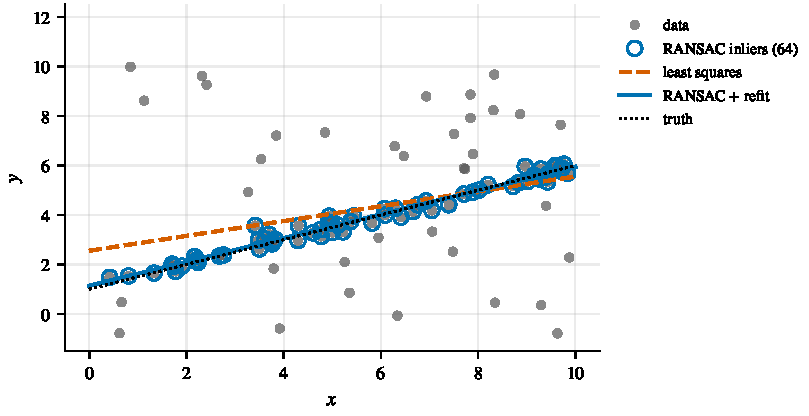
\includegraphics[width=0.86\textwidth]{fig_ransac.pdf}
  \caption{Fitting a line to data with 40\% gross outliers. Least squares is dragged away by the outliers; RANSAC finds the line supported by the most inliers
  (circled) and refits it to them.}
  \label{fig:ransac}
\end{figure}

% ==============================================================================
\section{Degeneracies}

\subsection{Pure rotation}

If the camera only rotates, $t = 0$ and $E = \sx{0}R = 0$: the epipolar constraint is satisfied by every pair of points, inlier or not. Under small translation the problem is
not degenerate but badly conditioned: $t$ is poorly determined, inlier sets fluctuate, and RANSAC may reject good tracks or accept bad ones. Hovering drones rotate in
place often, so this case must be handled (Milestone 9).

Under pure rotation the correspondences satisfy the stronger constraint $\bar x_2 \propto R\bar x_1$ (\cref{sec:homographies}), which does not involve $t$ at all. A robust front end
measures the parallax remaining after rotation compensation, for example the median of $\|\pi(R\bar x_1) - \pi(\bar x_2)\|$ over the tracks:
\begin{itemize}
  \item if it is large, run essential-matrix (or two-point) RANSAC;
  \item if it is tiny, skip epipolar RANSAC and reject only tracks that violate the rotation-only prediction $\bar x_2 \propto R\bar x_1$, with $R$ from the gyroscope.
\end{itemize}
Either way the system keeps tracking: low parallax means the features carry little information about translation, not that they are wrong. The MSCKF update
handles them gracefully, because their nullspace-projected residuals simply contribute little.

\subsection{Other degeneracies}

The eight-point algorithm is degenerate when all points lie on a plane, a common situation (floors, walls), because a homography then explains the data equally well;
the five-point algorithm is not. Very distant points behave like points at infinity and carry only rotational information. Moving objects form a second, consistent
rigid motion that RANSAC can mistake for the dominant one if they fill the image.

% ==============================================================================
\section{Triangulation}
\label{sec:triangulation}

Given observations $z_i$ of a point in cameras with known poses $(R_{wc_i}, p_{wc_i})$, triangulation estimates its world position $p_f$.

\subsection{The midpoint method}

Each observation defines a ray $p_{wc_i} + \lambda_ir_i$ with direction $r_i = R_{wc_i}\bar x_i$. With noise the rays do not intersect. The midpoint method finds the point
closest to all rays in the least-squares sense: the distance of $p$ from ray $i$ is $\|(I - \hat r_i\hat r_i\T)(p - p_{wc_i})\|$ with $\hat r_i$ the unit direction, so
\begin{equation}
  \Big(\sum_i(I - \hat r_i\hat r_i\T)\Big)\,p = \sum_i(I - \hat r_i\hat r_i\T)\,p_{wc_i} .
\end{equation}
It is simple and geometric, but it minimizes 3D distances rather than image errors, which weights distant views wrongly.

\subsection{Linear triangulation}

In camera $i$ the point has coordinates $X_i = R_{wc_i}\T(p_f - p_{wc_i})$, which must be parallel to the bearing $\bar x_i = (z_i, 1)$: $\sx{\bar x_i}X_i = 0$. Substituting,
\begin{equation}
  \sx{\bar x_i}R_{wc_i}\T\, p_f = \sx{\bar x_i}R_{wc_i}\T\, p_{wc_i}, \qquad i = 1,\dots,M .
  \label{eq:dlt}
\end{equation}
Each view contributes three equations of rank two. Stacking all views gives an overdetermined linear system $A p_f = b$ that is solved in the least-squares sense with
QR or SVD. With two views and noise-free data the solution is exact. This is the linear initialization of AGENTS.md F5. It minimizes an algebraic error, not the
reprojection error, so it is refined next.

\subsection{Nonlinear refinement with inverse depth}

The maximum-likelihood estimate minimizes the reprojection error (\cref{ch:nlls})
\begin{equation}
  \min_{p_f}\ \sum_{i=1}^M \big\| z_i - \pi(X_i(p_f)) \big\|^2 .
\end{equation}
The MSCKF~\cite{mourikis2007msckf} parameterizes the point in an \emph{anchor} camera $A$ (for example the first observation) by inverse depth~\cite{civera2008inverse}:
\begin{equation}
  X_A = \frac1\rho\begin{bmatrix} \alpha \\ \beta \\ 1 \end{bmatrix}, \qquad
  X_i = R_{iA}X_A + p_{iA}
  \quad\Longrightarrow\quad
  h_i := \rho X_i = R_{iA}\begin{bmatrix}\alpha\\ \beta\\ 1\end{bmatrix} + \rho\,p_{iA}, \quad z_i = \pi(h_i),
\end{equation}
where $(R_{iA}, p_{iA})$ is the transformation from the anchor camera to camera $i$, computed from the clone poses, and $\pi(h_i) = \pi(X_i)$ because projection ignores scale.
The parameters $(\alpha, \beta)$ are the normalized coordinates in the anchor view and $\rho = 1/Z_A$ is the inverse depth. This parameterization behaves well for distant points
($\rho\to0$ is a regular point), and the measurement function is nearly linear in $(\alpha, \beta, \rho)$. Its Jacobian follows from the chain rule:
\begin{equation}
  \frac{\partial z_i}{\partial(\alpha, \beta, \rho)} = \frac{\partial\pi}{\partial h}\Big|_{h_i}\,
  \begin{bmatrix} r_1 & r_2 & p_{iA} \end{bmatrix},
\end{equation}
where $r_1, r_2$ are the first two columns of $R_{iA}$ and $\partial\pi/\partial h$ is \cref{prop:proj-jacobian}. Gauss--Newton (\cref{alg:gauss-newton}) iterates
$\delta y = -(J\T J)\inv J\T e$ with the stacked Jacobian $J$ and residual $e$, usually converging in a few iterations from the linear initialization. Levenberg--Marquardt
damping adds robustness.

\subsection{How accurate is triangulation?}

For two views separated by a baseline $b$ perpendicular to the viewing direction, the depth is $Z = b/d$ with $d$ the disparity in normalized coordinates. With
independent noise $\sigma_{uv}$ in each view, $\sigma_d = \sqrt2\sigma_{uv}$, and since $\partial Z/\partial d = -b/d^2 = -Z^2/b$, to first order
\begin{equation}
  \sigma_Z \approx \frac{Z^2}{b}\sqrt2\,\sigma_{uv} .
  \label{eq:depth-sigma}
\end{equation}
Depth error grows quadratically with depth and inversely with baseline. Equivalently, the relative depth error is inversely proportional to the parallax angle $\approx b/Z$.

\begin{figure}[t]
  \centering
  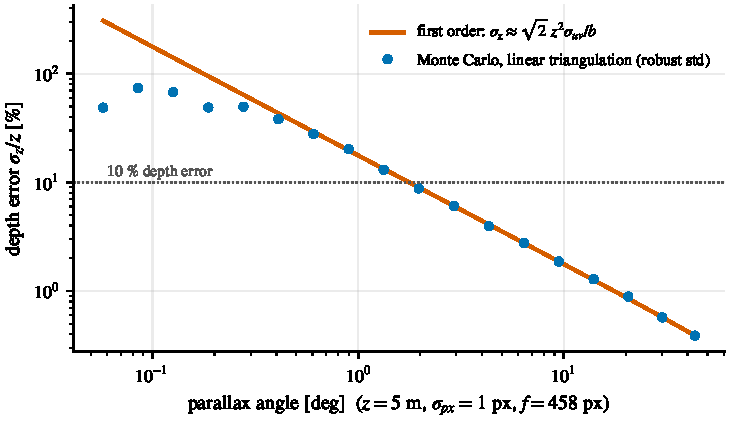
\includegraphics[width=0.86\textwidth]{fig_triangulation.pdf}
  \caption{Relative depth error of two-view triangulation at $Z = 5$~m with 1-pixel noise, versus parallax angle. Down to about $1^\circ$ the first-order formula \eqref{eq:depth-sigma}
  describes the spread accurately. Below that the error distribution becomes heavy-tailed (depths can even become negative), and the estimate is unusable.}
  \label{fig:triangulation}
\end{figure}

\Cref{fig:triangulation} shows that 10\% depth accuracy needs about $2^\circ$ of parallax, a baseline of 17~cm at 5~m. Down to about $1^\circ$ \eqref{eq:depth-sigma} still
describes the bulk of the estimates; below that, outliers take over. At $0.5^\circ$, 4\% of the estimates are off by more than five standard deviations, and at
$0.25^\circ$, 8\% of the depths come out negative. A triangulation module must therefore check its own result before handing it to the filter:
\begin{itemize}
  \item positive depth in every view (cheirality);
  \item sufficient parallax (or baseline relative to depth), or equivalently a well-conditioned Gauss--Newton Hessian;
  \item small reprojection error in every view after refinement;
  \item a plausible depth range.
\end{itemize}
Features that fail are discarded, not fed to the update (AGENTS.md F5, Milestone 10b).

% ==============================================================================
\section{Bundle adjustment}
\label{sec:bundle-adjustment}

\termi{Bundle adjustment}{bundle adjustment} estimates all camera poses and all 3D points at once by minimizing the total reprojection error,
\begin{equation}
  \min_{\{T_i\},\{p_j\}}\ \sum_{(i,j)\text{ observed}}\big\|z_{ij} - \pi\big(T_i\inv p_j\big)\big\|^2_{R\inv},
\end{equation}
with Gauss--Newton or Levenberg--Marquardt on the manifold of poses (\cref{ch:nlls}). It is the gold standard of geometric vision. Two of its properties illuminate
VIO.
\begin{itemize}
  \item \emph{Structure.} Each residual involves one camera and one point, so the normal equations have the block structure of \cref{sec:schur-ba}: eliminating the
        points with the Schur complement leaves a small \emph{reduced camera system} (\cref{fig:ba-sparsity}).
  \item \emph{Gauge freedom.} Moving and rotating everything together, or (for a monocular camera) scaling everything, leaves all reprojection errors unchanged: the
        problem has seven unobservable directions, and $J\T WJ$ is singular along them. Solvers fix the gauge by holding the first camera fixed and the scale constant, or
        by adding a weak prior. With an IMU, scale and two rotation directions (roll and pitch) become observable, and the gauge shrinks to the four directions of
        \cref{ch:observability}.
\end{itemize}
The MSCKF can be understood as a fast, filtered approximation of bundle adjustment over a sliding window: it eliminates each point exactly as the Schur complement
does (\cref{ch:msckfupdate}), takes a single Gauss--Newton step, and summarizes the past by the filter's Gaussian prior instead of relinearizing it.

\paragraph{Pose from known points.} Finally, when the 3D points are known (a map), a single image determines the camera pose: the
\emph{perspective-$n$-point} (PnP) problem, solved minimally from three points and refined by Gauss--Newton. It is the core of relocalization against a map, a
capability that odometry lacks.

\begin{takeaways}
\begin{itemize}
  \item Rigid correspondences satisfy $\bar x_2\T\sx{t}R\bar x_1 = 0$; $E$ has 5 DOF, singular values $(\|t\|, \|t\|, 0)$, and an unobservable scale.
  \item The eight-point algorithm is linear (normalize pixel coordinates first); $E$ decomposes into four motions, one of which passes the cheirality test.
  \item With the rotation from the gyroscope, two correspondences determine the translation direction.
  \item Planes and pure rotations relate views by homographies; under pure rotation $E$ vanishes and the rotation-only constraint takes over.
  \item RANSAC iterations grow as $w^{-s}$: prefer minimal solvers. Thresholds in normalized units are $\tau_{px}/f$.
  \item Triangulate linearly, refine by Gauss--Newton with inverse depth, and reject low-parallax or negative-depth points; depth error grows as $Z^2/b$.
  \item Bundle adjustment is the batch problem; the MSCKF approximates it with exact landmark elimination and a single Gauss--Newton step.
\end{itemize}
\end{takeaways}

\begin{exercises}
  \item Verify \cref{thm:epipolar} numerically for random points and a random relative pose, then show that adding an outlier breaks it.
  \item Prove \cref{prop:essential} and show that $e_2 \propto t$ is the left null vector of $E$.
  \item Implement the eight-point algorithm with and without Hartley normalization on pixel coordinates, and compare the errors.
  \item Implement the decomposition of \cref{prop:e-decomposition} and the cheirality test, and verify on synthetic data that the correct solution is selected.
  \item Implement the two-point method with known rotation inside RANSAC on synthetic data with 30\% outliers. Compare the number of iterations needed with the five-point
        method.
  \item Generate a pure-rotation sequence, observe what \code{cv::findEssentialMat} returns, and implement the parallax test.
  \item Show that \eqref{eq:dlt} has rank two per view and that two views with non-parallel rays give a unique solution.
  \item Derive \eqref{eq:depth-sigma}, reproduce \cref{fig:triangulation}, and repeat with three views over the same baseline.
  \item Count the gauge freedoms of monocular bundle adjustment and of visual-inertial bundle adjustment, and explain the difference.
\end{exercises}
% Solutions to the exercises of Chapter 23.
\begin{solutions}
  \item With 20 random points at 3--8~m and a random relative pose, $|\bar x_2\T E\bar x_1| \le 3\times10^{-17}$: rounding error. Moving one observation in the second image
        by 27~px gives an algebraic residual of $8\times10^{-3}$ and a Sampson distance $\sqrt{d_S}$ of $5.4$~px. Only the component of the error perpendicular to the
        epipolar line is visible (7.7~px of the 27~px here), and the Sampson distance spreads it over both images ($7.7/\sqrt2 = 5.4$). A two-view check cannot
        detect an error \emph{along} the epipolar line at all; a third view, or the filter's own gating, must catch those.

  \item Since $RR\T = I$ and $\sx{t}\T = -\sx{t}$, $EE\T = -\sx{t}^2 = \|t\|^2I - tt\T$ (\eqref{eq:skew-sq}). Every vector orthogonal to $t$ is an eigenvector with eigenvalue
        $\|t\|^2$, and $t$ itself has eigenvalue 0, so the singular values of $E$ are $(\|t\|, \|t\|, 0)$ and its rank is two. Degrees of freedom: $R$ has three and $t$ three,
        but the constraint $\bar x_2\T E\bar x_1 = 0$ is homogeneous, so $E$ and $\lambda E$ (i.e.\ $t$ and $\lambda t$) are indistinguishable: $3 + 2 = 5$. Scaling the scene and
        the baseline together leaves every bearing unchanged, so the scale of $t$ cannot be recovered from images. For the epipoles,
        \[
          t\T E = t\T\sx{t}R = -(\sx{t}t)\T R = -(t\times t)\T R = 0, \qquad E(R\T t) = \sx{t}t = 0 .
        \]
        The left null vector is $t$, the coordinates of the first camera center in the second frame ($X_1 = 0 \Rightarrow X_2 = t$), so $e_2 \propto t$ is its image. Likewise
        $e_1 \propto R\T t$ is the image of the second center ($X_2 = 0 \Rightarrow X_1 = -R\T t$).

  \item With 60 points, 0.5~px noise and 200 random scenes, recovering $(R, t)$ from $E = K\T FK$:
        \begin{center}\small
        \begin{tabular}{@{}l c c c@{}}
        \toprule
        & $\sigma_1/\sigma_8$ of $A$ & rotation error & direction of $t$ \\
        & & median / 90\% & median / 90\% \\
        \midrule
        raw pixels & $1.5\times10^5$ & $0.33^\circ$ / $1.6^\circ$ & $2.5^\circ$ / $11^\circ$ \\
        Hartley-normalized & 66 & $0.16^\circ$ / $0.34^\circ$ & $1.1^\circ$ / $2.4^\circ$ \\
        \bottomrule
        \end{tabular}
        \end{center}
        In pixels, the columns of $A$ range from $1$ to $10^5$, so the smallest singular vector is dominated by rounding and by the noise in the large entries.
        Normalization makes all columns comparable. It halves the typical error and removes the bad cases, which matter most inside RANSAC.

  \item Take the SVD of $E$, flip the sign of $U$ or $V$ if its determinant is $-1$ (allowed, since $E$ is defined up to sign), and form the four candidates. For each,
        triangulate every correspondence (two depths from $\lambda_2\bar x_2 = \lambda_1R\bar x_1 + t$ by least squares) and count the points with both depths positive. In 500 random
        scenes, the true solution won every time, with all points in front of both cameras. For each wrong candidate, \emph{all} points failed: in a typical scene one
        candidate put them in front of the first camera but behind the second, and the other two put them behind the first. With noisy data, use the count, not
        a requirement that every point pass.

  \item With $R$ known, each correspondence gives $c_i = R\bar x_1^{(i)}\times\bar x_2^{(i)}$, the hypothesis is $t \propto c_i\times c_j$, and inliers have $\sqrt{d_S}$ below the threshold (2~px).
        For 100 correspondences with 1-pixel noise and 30\% outliers, adaptive RANSAC stopped after 9.8 iterations on average ($\lceil\log0.01/\log(1 - 0.7^2)\rceil = 7$
        at the true ratio; the observed ratio is slightly lower because the threshold rejects some inliers). After refitting $t$ to all inliers (the unit $t$
        minimizing $\sum(t\T c_i)^2$), the median direction error was $0.6^\circ$; 4.6\% of the inliers were rejected (the expected rate of a $2\sigma$ threshold) and 1.3\% of the
        outliers accepted (those lying near their epipolar line by chance). The five-point method needs $\lceil\log0.01/\log(1 - 0.7^5)\rceil = 26$ iterations at the same confidence,
        each solving a degree-10 polynomial and scoring up to ten candidates, against one cross product. The price of the two-point method is its dependence
        on the gyroscope: a rotation error $\delta$ shifts predicted points by about $f\delta$ pixels, so the threshold must cover the gyro error accumulated between
        frames.

  \item With $t = 0$, every correspondence satisfies $\bar x_2 \propto R\bar x_1$, so $\bar x_2\T\sx{t}R\bar x_1 = \bar x_2\T(t\times R\bar x_1) = 0$ for \emph{every} $t$. The data fit the
        whole family $E = \sx{t}R$, and the eight-point matrix $A$ has three singular values at the noise level instead of one. In simulation, a randomly chosen
        $t$ combined with the true $R$ fits 68--70\% of the tracks to within 1~px, exactly the fraction the true model fits with 1-pixel noise. Whatever
        \code{cv::findEssentialMat} returns therefore has an arbitrary translation direction that changes from run to run, and its inlier set is no test of the
        tracks, since the free $t$ can turn epipolar lines through outliers. The parallax test: the median of $\|\pi(R\bar x_1) - \pi(\bar x_2)\|$ over the tracks was
        $1.6$~px under pure rotation (noise only) and $8.8$~px for a 10~cm sideways motion with points at 3--8~m. A threshold of a few pixels separates the two
        regimes. Below it, check tracks only against $\bar x_2 \propto R\bar x_1$.

  \item The matrix $\sx{\bar x_i}$ has rank two (its nullspace is $\bar x_i$), and multiplying by the invertible $R_{wc_i}\T$ keeps the rank, so each view contributes three
        equations of rank two. For two views, $p$ is in the nullspace of the stacked matrix if and only if $R_{wc_i}\T p \parallel \bar x_i$ for both views, i.e.\ $p$ is parallel to both ray
        directions $r_i = R_{wc_i}\bar x_i$. If the rays are not parallel, only $p = 0$ qualifies: the $6\times3$ matrix has full column rank, and the least-squares solution
        is unique. Parallel rays (zero parallax) leave a one-dimensional nullspace, the position along the ray.

  \item With the baseline perpendicular to the viewing direction, $Z = b/d$ with disparity $d = x_1 - x_2$. The two noises are independent, so $\sigma_d = \sqrt2\sigma_{uv}$, and to first
        order $\sigma_Z = |\partial Z/\partial d|\,\sigma_d = (b/d^2)\sqrt2\sigma_{uv} = (Z^2/b)\sqrt2\sigma_{uv}$. A Monte Carlo at $Z = 5$~m with 1-pixel noise reproduces the figure: relative errors
        of $17.7\%$, $8.8\%$, $3.5\%$, $1.8\%$ at parallax angles of $1^\circ$, $2^\circ$, $5^\circ$, $10^\circ$, matching the formula. For three views at $0$, $b/2$ and $b$, write the
        observations as $x_i = X/Z - s_i/Z + n_i$, with $s_i$ the camera positions along the baseline. The inverse depth $1/Z$ is the \emph{slope} of a straight-line fit of $x_i$
        against $s_i$, with variance $\sigma_{uv}^2/\sum_i(s_i - \bar s)^2$. A view at the mean position $\bar s$ adds nothing to this sum: three views give the same depth accuracy as
        two (simulation: within 2\%), and five equally spaced views improve it by only 11\%. Depth accuracy is bought with baseline; intermediate views
        add redundancy, which is what outlier detection and the MSCKF's nullspace projection need.

  \item Monocular bundle adjustment has seven gauge freedoms: a global translation (3), a global rotation (3) and a global scale (1) leave all reprojection errors
        unchanged. Visual--inertial bundle adjustment has four: translation (3) and rotation about the gravity direction (1). The accelerometer measures
        specific force in the body frame, and the residuals compare it with $R_{wb}\T(a_w - g_w)$ for the fixed $g_w$. A global rotation about a horizontal axis would tilt the
        trajectory relative to gravity and change these residuals, so roll and pitch are observable. A rotation about the vertical leaves $g_w$ invariant and
        changes nothing. Scale becomes observable because the IMU measures metric accelerations, which a scaled trajectory would contradict, provided
        the motion actually accelerates (at constant velocity, scale is unobservable again). Consequently, fix the gauge of a visual--inertial problem with
        the first position and yaw only: fixing roll and pitch as well would inject false information.
\end{solutions}



\part{The Multi-State Constraint Kalman Filter}
\chapter{From EKF-SLAM to the MSCKF}
\label{ch:msckfintro}

\begin{objectives}
\begin{itemize}
  \item Understand how EKF-SLAM uses visual landmarks, and why it scales poorly.
  \item Understand the central idea of the MSCKF: constraints between multiple past poses instead of landmarks.
  \item See why past poses must be kept in the state, with their correlations.
  \item Relate the MSCKF to sliding-window optimization.
\end{itemize}
\end{objectives}

% ------------------------------------------------------------------------------
\section{EKF-SLAM}

\index{EKF-SLAM}
The most direct way to use a camera in an EKF is to put the landmarks in the state. With $L$ landmarks,
\begin{equation}
  x = \big(x_I,\ p_{f_1},\ \dots,\ p_{f_L}\big), \qquad \dim\delta x = 15 + 3L,
\end{equation}
and each image observation $z = \pi(p_c(x_I, p_{f_j})) + n$ is an ordinary EKF measurement of the IMU state and one
landmark. This is EKF-SLAM, and MonoSLAM~\cite{davison2007monoslam} showed it can run in real time with a single camera.

\subsection{How it works}

\paragraph{Prediction.} Landmarks are static, so only the IMU block is propagated: exactly the block structure of clones in \cref{ch:errordyn},
$P_{II} \gets \Phi P_{II}\Phi\T + Q_d$, $P_{IL} \gets \Phi P_{IL}$, with the landmark block unchanged.

\paragraph{Update.} An observation of landmark $j$ has a Jacobian with two non-zero blocks: one for the IMU pose and one for landmark $j$,
$H = [H_I\ \ 0\ \cdots\ 0\ \ H_{f_j}\ \ 0\ \cdots]$. The gain $K = PH\T S\inv$ is nevertheless dense: every landmark correlated with the robot or with landmark $j$ is corrected.
This is how EKF-SLAM ``closes loops'': re-observing an old landmark corrects the robot, which through the correlations corrects every other landmark. It is also
what makes it expensive.

\paragraph{Landmark initialization.} A new landmark enters the state as a function of the current state and the first measurement, $p_f = g(x_I, z)$. This is the
state augmentation of \cref{prop:augmentation}: $P \gets JPJ\T + J_zRJ_z\T$ with $J = [I;\ \partial g/\partial x]$ and $J_z = [0;\ \partial g/\partial z]$. For a monocular camera, $g$
needs a depth that a single measurement does not provide, which leads to the initialization problem below.

\subsection{Why it scales poorly}

EKF-SLAM has three structural problems.
\begin{enumerate}
  \item \textbf{Cost.} The covariance has $(15 + 3L)^2$ entries, and every update touches all of them: the Joseph update costs $\mathcal{O}(n^2)$ per scalar measurement at
        best. Tracking 200 landmarks gives a $615\times615$ covariance; updating it at 20~Hz with hundreds of observations per frame is expensive, and the cost
        grows quadratically with the map.
  \item \textbf{Initialization.} A single monocular observation says nothing about depth. A new landmark must be
        initialized with a huge depth uncertainty, which is highly non-Gaussian in Euclidean coordinates, or its
        initialization must be delayed until it has been seen from several viewpoints. Inverse-depth
        parameterizations~\cite{civera2008inverse} help, but add complexity.
  \item \textbf{Housekeeping.} Landmarks that leave the field of view must either stay in the state, growing it, or be
        marginalized, which in covariance form is cheap but discards their future value.
\end{enumerate}

% ------------------------------------------------------------------------------
\section{The multi-state constraint}
\index{multi-state constraint}\index{MSCKF}

Consider a feature observed in $M$ images taken at times $t_1, \dots, t_M$. Each observation constrains the pose at its
time and the feature position. Taken together, after the unknown feature position is eliminated, the $2M$ observations
impose $2M - 3$ constraints \emph{on the $M$ poses alone}. This is the \emph{multi-state constraint}: geometric information
about how the camera moved between the images, with the scene point serving only as an intermediary.

\begin{keyidea}[the MSCKF in one sentence]
Keep a sliding window of past poses in the state instead of landmarks; when a feature track is complete,
triangulate it, linearize its observations, and eliminate the feature by projecting onto the left nullspace of its
Jacobian, leaving a residual that depends only on the poses; then update.
\end{keyidea}

Mourikis and Roumeliotis~\cite{mourikis2007msckf} showed that this uses all the information that the observations carry about
the poses (under linearization), at a cost linear in the number of features. Feature positions are never part of the
state, so there is no landmark initialization problem inside the filter, and features leaving the view simply trigger an
update.

\section{Why past poses must be in the state}

Why not keep only the current IMU state and use the constraint between the current pose and the past ones? Because the
past poses are \emph{estimated} quantities, with errors correlated with the current state's error: they were all produced by
the same propagation from the same measurements. A measurement relating the current pose to a past pose estimate, which
treats that past estimate as fixed or independent, double counts information and makes the filter overconfident.

The cure is \emph{stochastic cloning}~\cite{roumeliotis2002cloning}. When an image is captured, a copy of the current pose (a
clone) is appended to the state, together with its exact correlations to everything else. From then on the clone is a
state variable whose estimate can be corrected by later measurements, and whose correlation with the evolving IMU state is
propagated exactly. \Cref{ch:cloning} develops this in detail.

\begin{figure}[t]
\centering
\begin{tikzpicture}[scale=1.0]
  % trajectory
  \draw[->, thick, black!50] (-0.5,-0.2) .. controls (2,0.6) and (5,0.7) .. (9.4,0.1) node[right, font=\footnotesize] {time};
  % clones
  \foreach \x/\y/\a/\n in {0.3/0.02/12/1, 1.8/0.33/9/2, 3.3/0.5/5/3, 4.8/0.56/0/4, 6.3/0.5/-5/5, 7.8/0.33/-10/6} {
    \begin{scope}[shift={(\x,\y)}, rotate=\a]
      \draw[fill=primarylight, draw=primary] (-0.2,0) -- (0.2,0) -- (0.3,0.42) -- (-0.3,0.42) -- cycle;
    \end{scope}
    \node[font=\scriptsize, below=2pt] at (\x,\y) {$C_\n$};
  }
  % current IMU
  \fill[conv] (9.0,0.15) circle (2.5pt) node[below=3pt, font=\scriptsize] {IMU state};
  % features
  \coordinate (F1) at (2.4,3.2); \coordinate (F2) at (5.6,3.6); \coordinate (F3) at (7.6,2.9);
  \fill[plotgreen] (F1) circle (2.3pt) node[above] {\footnotesize $f_1$};
  \fill[plotgreen] (F2) circle (2.3pt) node[above] {\footnotesize $f_2$};
  \fill[plotgreen] (F3) circle (2.3pt) node[above] {\footnotesize $f_3$};
  \foreach \x/\y in {0.3/0.44, 1.8/0.75, 3.3/0.92} \draw[plotgreen, dashed] (\x,\y) -- (F1);
  \foreach \x/\y in {3.3/0.92, 4.8/0.98, 6.3/0.92, 7.8/0.75} \draw[plotgreen!60!black, dashed] (\x,\y) -- (F2);
  \foreach \x/\y in {6.3/0.92, 7.8/0.75} \draw[plotorange, dashed] (\x,\y) -- (F3);
  \draw[decorate, decoration={brace, amplitude=5pt, mirror}] (0,-0.55) -- (8.1,-0.55) node[midway, below=6pt, font=\footnotesize] {sliding window of $N$ clones (poses at image times), all in the state};
\end{tikzpicture}
\caption{The MSCKF state: the current IMU state plus clones of past camera poses. Feature $f_1$ is seen by clones 1--3
and constrains them; $f_2$ by clones 3--6. Neither feature is in the state. Feature $f_3$ has only two observations so far
and keeps being tracked.}
\label{fig:msckf-window}
\end{figure}

% ------------------------------------------------------------------------------
\section{The MSCKF state}

The project's state (AGENTS.md C3) is the IMU state plus $N \le$ \code{kMaxClones} clones, each holding the IMU pose
$(p_{wb}, q_{wb})$ at an image timestamp:
\begin{equation}
  x = \big(\,p,\ v,\ q,\ b_a,\ b_g,\ \ p_1, q_1,\ \dots,\ p_N, q_N\,\big),\qquad \dim\delta x = 15 + 6N .
\end{equation}
The camera pose of clone $i$ is derived through the fixed extrinsics,
$R_{wc_i} = R_{wb_i}R_{bc}$ and $p_{wc_i} = p_{wb_i} + R_{wb_i}p_{bc}$. With \code{kMaxClones} $= 10$, the error state has 75
dimensions, independent of how many features are tracked.

% ------------------------------------------------------------------------------
\section{Relation to sliding-window optimization}

Optimization-based VIO (OKVIS~\cite{leutenegger2015okvis}, VINS-Mono~\cite{qin2018vins}) keeps a similar window of poses and
minimizes the sum of squared reprojection and IMU residuals over poses \emph{and} landmarks, relinearizing at every
iteration, then marginalizes old states into a Gaussian prior. The MSCKF update is equivalent to a single Gauss--Newton
iteration of such a problem, with the landmarks eliminated by a Schur complement and the prior given by the filter's
covariance. Eliminating a landmark by nullspace projection and by Schur complement give the same information about the
poses (\cref{thm:nullspace-optimal}). The differences are that the MSCKF never relinearizes past measurements, and
processes each feature track exactly once, which makes it cheaper and more predictable, at some cost in accuracy under
strong nonlinearity.

\section{Variants}

The basic MSCKF has been refined in many directions. MSCKF 2.0~\cite{li2013msckf2} added First-Estimates Jacobians for
consistency and online calibration of extrinsics and time offset. Hybrid filters keep long-lived features in the state as
SLAM landmarks while processing short tracks MSCKF-style. MSCKF-VIO~\cite{sun2018msckfvio} uses a stereo camera and
two-point RANSAC for fast flight, and OpenVINS~\cite{geneva2020openvins} is a modular research platform that implements most of
these options and documents them carefully.

\begin{takeaways}
\begin{itemize}
  \item EKF-SLAM keeps landmarks in the state; its cost grows quadratically with the map.
  \item The MSCKF keeps past poses (clones) instead; each feature track is turned into constraints on those poses.
  \item Past poses must be in the state, with their correlations, or information is double counted.
  \item The MSCKF update is equivalent to one Gauss--Newton step of sliding-window bundle adjustment with landmarks
        marginalized.
\end{itemize}
\end{takeaways}

\begin{exercises}
  \item Estimate the memory and the per-update flop count of EKF-SLAM with 200 landmarks and of the MSCKF with 10 clones.
  \item A feature is observed in $M$ images. How many scalar constraints does it impose on the poses? Why does the count
        start being useful only at $M = 2$, and why does the project require $M \ge 3$?
  \item Explain in your own words why using a past pose estimate as if it were known exactly makes the filter
        overconfident. Construct a scalar example.
\end{exercises}

\chapter{Stochastic Cloning and the Sliding Window}
\label{ch:cloning}
\chaptermark{Stochastic Cloning} % short running header

\begin{objectives}
\begin{itemize}
  \item See, on a scalar example, why relative measurements require cloned states with correlations.
  \item Derive the general state-augmentation formula $P \gets JPJ\T$.
  \item Derive the project's cloning Jacobian and the invariance property of cloning.
  \item Marginalize the oldest clone in place without allocation, and choose a window policy and size.
\end{itemize}
\end{objectives}

% ------------------------------------------------------------------------------
\section{A scalar example}

Let $x$ be a scalar position that performs a random walk, $x_{k+1} = x_k + w_k$ with $\Var(w_k) = Q$, and suppose its
current estimate has variance $P$. At time 1 we \emph{clone} it, $x_c := x_1$; between times 1 and 2 the state moves; then a
sensor measures the displacement:
\begin{equation}
  z = x_2 - x_c + n, \qquad \Var(n) = R .
\end{equation}
Augmenting the state with the clone gives the vector $(x, x_c)$. At the moment of cloning both entries are the \emph{same}
random variable, so their joint covariance is $\begin{bmatrix} P & P \\ P & P\end{bmatrix}$, which is singular. Propagating $x$ but
not $x_c$ gives
\begin{equation}
  P_{\mathrm{aug}} = \begin{bmatrix} P + Q & P \\ P & P \end{bmatrix}, \qquad H = \begin{bmatrix} 1 & -1 \end{bmatrix}.
\end{equation}
The innovation covariance and gain are
\begin{equation}
  S = (P + Q) - 2P + P + R = Q + R, \qquad K = \frac{1}{Q + R}\begin{bmatrix} Q \\ 0 \end{bmatrix}.
\end{equation}
The result is exactly right: a displacement measurement is informative only about what happened \emph{between} the two
times, so $S$ involves only $Q$ and $R$. The update corrects the current state by the part of its uncertainty that arose
after the clone, and leaves the clone untouched. The posterior variance of $x_2$ is $P + Q - Q^2/(Q + R)$, which stays
large if $P$ is large, as it must: a relative measurement cannot reveal absolute position.

Now suppose we had treated the past estimate as known (no clone, zero variance). Then $S = P + Q + R$ and the posterior
variance of $x_2$ would be $(P + Q)R/(P + Q + R)$, which tends to $R$ when $P$ is large. The filter would believe it had
learned the absolute position to within the sensor noise from a displacement measurement: a severe overconfidence.
Treating the past estimate as an independent random variable is wrong in a different way. Only the exact
cross-covariance gives the right answer, and stochastic cloning~\cite{roumeliotis2002cloning} is the mechanism that keeps it.

% ------------------------------------------------------------------------------
\section{State augmentation}

\begin{proposition}[Augmentation with a function of the state]
\label{prop:augmentation}
Let $x$ have error covariance $P$, and append a new variable $y = g(x)$ whose error satisfies $\delta y \approx J_g\,\delta x$. The
augmented error $(\delta x, \delta y) = J\,\delta x$ with $J = \begin{bmatrix} I \\ J_g\end{bmatrix}$ has covariance
\begin{equation}
  P \gets J P J\T = \begin{bmatrix} P & PJ_g\T \\ J_gP & J_gPJ_g\T \end{bmatrix}.
  \label{eq:augmentation}
\end{equation}
\end{proposition}
\begin{proof}
\Cref{prop:affine} with the linear map $J$.
\end{proof}

The augmented covariance has rank $\dim x$: it is singular, because $y$ is a deterministic function of $x$ at the moment of
augmentation. This is correct and harmless. Propagation adds process noise to the IMU block only, after which the clone and
the current state are no longer perfectly correlated. The Joseph form and symmetrization keep the matrix positive
semi-definite throughout.

\section{The project's clone}

At an image timestamp, after propagating the IMU state to exactly that time, the filter appends a clone holding the current
pose $(p_{wb}, q_{wb})$, and augments the covariance with the cloning Jacobian (AGENTS.md F5).

\begin{derivex}{the cloning Jacobian $J$}{sol:clone}
The clone's error is defined with the same retraction as the IMU pose (AGENTS.md C4): $p_c = \hat p_c + \delta p_c$ and
$q_c = \hat q_c\qprod\Exp_q(\delta\theta_c)$, with $\hat p_c = \hat p$ and $\hat q_c = \hat q$ at cloning time.
\begin{enumerate}
  \item At the moment of cloning the true clone equals the true IMU pose. Express $\delta p_c$ and $\delta\theta_c$ in terms of the IMU
        error state. Is any linearization needed?
  \item Write $J_g \in \R^{6\times(15+6N)}$ and then $J \in \R^{(21+6N)\times(15+6N)}$, with the new clone appended at the end of the
        state.
  \item What would change if the clone stored the \emph{camera} pose $(p_{wc}, q_{wc})$ instead of the IMU pose? (The project
        deliberately does not do this.)
\end{enumerate}
\textbf{Check:} Milestone 10a requires that after cloning, the new clone's covariance block and its cross-covariances equal the
corresponding IMU pose blocks \emph{exactly}, and that a run with cloning enabled but only pose updates reproduces the
IMU estimate and covariance of a run without cloning to $10^{-10}$.
\end{derivex}

\begin{proposition}[Cloning does not change the IMU marginal]
\label{prop:clone-invariance}
Augmentation, propagation with static clones, and marginalization of clones leave the marginal distribution of the IMU state
unchanged, provided no measurement involves the clones.
\end{proposition}
\begin{proof}
Augmentation leaves the $P_{II}$ block unchanged by \eqref{eq:augmentation}. Propagation updates $P_{II}$ by $\Phi P_{II}\Phi\T + Q_d$
regardless of the clones. Marginalization deletes clone rows and columns. A measurement that involves only the IMU state
has a Jacobian with zero clone columns; its gain for the IMU block, $P_{II}H_I\T S\inv$, and $S = H_IP_{II}H_I\T + R_z$ do not
involve the clones either.
\end{proof}

This is the invariance test of Milestone 10a. It is a powerful end-to-end check of the augmentation, propagation and
marginalization code, because any indexing error in the clone blocks leaks into the IMU block and breaks the equality.

% ------------------------------------------------------------------------------
\section{Clones in propagation and updates}

Clones are static (\cref{ch:errordyn}): propagation multiplies their cross-covariance with the IMU state by $\Phi$ and leaves the
clone-clone block alone. Visual measurements depend only on clone states, so their Jacobians are zero in the IMU columns.
The update nevertheless corrects the IMU state, through the gain rows $P_{IC}H_C\T S\inv$: information about relative motion
between past poses corrects the current velocity, attitude and biases through the correlations built up by propagation.
Injection and reset (\cref{sec:reset}) apply to every clone, each with its own $I - \tfrac12\sx{\delta\hat\theta_i}$ block.

% ------------------------------------------------------------------------------
\section{Marginalizing the oldest clone}

When the window holds \code{kMaxClones} clones and a new image arrives, the oldest clone must go. In covariance form,
marginalization is deletion of its six rows and columns (\cref{thm:gauss-cond}). Before deleting it, the filter must process
every feature that has an observation at that clone (AGENTS.md F5), because those observations become unusable once
the clone is gone.

\begin{implnote}[in-place deletion without allocation]
$P$ is stored in a fixed-max-size matrix whose active part is the top-left $n\times n$ corner. Deleting the block at offset $o$
means shifting every row below it up by six and every column to its right left by six, then reducing $n$ by six. The source
and destination regions overlap. Copying toward lower indices in ascending order is safe, because each element is read
before it is overwritten (\code{std::copy} permits overlapping ranges when the destination begins before the source), but an
Eigen block assignment between overlapping blocks of the same matrix is an aliasing hazard whose traversal order is not
guaranteed. Write the shift explicitly, or through a preallocated member workspace, and test it against a reference built
with a dynamic matrix (Milestone 10a).
\end{implnote}

The clone states themselves are stored in a fixed-capacity container, such as a ring buffer of $N_{max}$ poses with
timestamps, so that removing the oldest is a pointer move. If the covariance blocks are kept in the same order as the
container, a ring-buffer layout could even avoid the shift, at the cost of more complex index arithmetic. Simplicity is
usually the better choice here: the shift costs $\mathcal{O}(n^2)$ once per image.

% ------------------------------------------------------------------------------
\section{Window policy and size}

The project uses the simplest policy: first in, first out. Each image creates a clone, and the oldest is marginalized when
the window is full. More elaborate policies keep clones that are geometrically useful: if the vehicle barely moved since the
previous image, marginalize the second-newest clone instead of the oldest, so that the window spans a longer baseline.

The window size trades accuracy for cost.
\begin{itemize}
  \item \textbf{Longer windows} let longer tracks be used in full, with more parallax, and give each update more
        constraints.
  \item \textbf{Cost} grows as $\mathcal{O}(n^3)$ per update with $n = 15 + 6N$, and as $\mathcal{O}(n^2)$ per IMU step for the
        cross-covariance propagation.
  \item \textbf{Memory}: a fixed-max covariance of doubles occupies $8(15 + 6N_{max})^2$ bytes: 45~kB for $N_{max} = 10$, 146~kB for
        20, 304~kB for 30. Workspaces for $H$, $S$ and $K$ add similar amounts.
\end{itemize}

\begin{pitfall}[the stack budget]
Fixed-max-size Eigen matrices store their maximum-size buffer \emph{inline}, with no heap allocation. That is what makes them
allocation-free, but it also means a filter object constructed on the stack carries all of its matrices on the stack. With
the default 1~MB main-thread stack on Windows, a filter with a few hundred kilobytes of workspaces can overflow it. Construct
the filter once, during the load phase, as a heap object (for example with \code{std::make\_unique}), which the memory tiers
allow, and keep the large matrices as members rather than function-local temporaries (AGENTS.md E4, Milestone 10a).
\end{pitfall}

\begin{takeaways}
\begin{itemize}
  \item A relative measurement between a past and a present state needs the past state in the filter, with its exact
        correlations. Treating the past estimate as known makes the filter overconfident.
  \item Augmentation with $y = g(x)$ uses $P \gets JPJ\T$, $J = [I; J_g]$; the result is singular at first and becomes regular
        after propagation.
  \item Cloning, static propagation and marginalization leave the IMU marginal unchanged; this is a strong test.
  \item Marginalizing a clone deletes its rows and columns, after first processing its features. Shift in place carefully.
  \item Fixed-max matrices live inline: keep them as members of a heap-allocated filter.
\end{itemize}
\end{takeaways}

\begin{exercises}
  \item In the scalar example, compute the posterior covariance of $(x_2, x_c)$ and verify that the clone's variance is
        unchanged. When would a relative measurement change the clone's estimate?
  \item Extend the scalar example to two clones and two displacement measurements, and show that processing them gives the
        same result as one measurement of $x_2 - x_{c_1}$ followed by one of $x_{c_2} - x_{c_1}$, if correlations are kept.
  \item Implement in-place deletion of a $6\times6$ block from a $75\times75$ symmetric matrix stored in a larger buffer, and test it
        against a reference.
  \item For $N_{max} = 10, 20, 30$, estimate the flop count of one MSCKF update with 50 features of 6 observations each, with and
        without QR compression (\cref{ch:msckfupdate}).
\end{exercises}
% Solutions to the exercises of Chapter 25.
\begin{solutions}
  \item With $H = [1\ \ -1]$, $HP_{\mathrm{aug}} = [\,Q\ \ 0\,]$ and $K = [Q\ \ 0]\T/(Q + R)$, so
        \[
          P^+ = P_{\mathrm{aug}} - KHP_{\mathrm{aug}} = \begin{bmatrix} P + Q - \dfrac{Q^2}{Q + R} & P \\[1ex] P & P \end{bmatrix}.
        \]
        The clone's variance and its covariance with $x_2$ are unchanged ($P = Q = R = 1$ gives $\big[\begin{smallmatrix} 1.5 & 1 \\ 1 & 1\end{smallmatrix}\big]$). The clone's gain is
        $\Cov(x_c, x_2 - x_c)/S$, and here $x_2 - x_c = w$ is independent of $x_c$. A relative measurement corrects the clone whenever this covariance is not zero:
        if an absolute measurement of $x_2$ was made after cloning, if the dynamics are not a pure random walk ($x_2 = ax_1 + w$ with $a \ne 1$), or if other correlated
        states such as a velocity link them. For example, after an absolute fix of $x_2$ with unit variance the covariance is $\tfrac13\big[\begin{smallmatrix} 2 & 1 \\ 1 & 2\end{smallmatrix}\big]$, the
        relative measurement's gain is $(0.2, -0.2)$, and the clone's variance falls from $0.67$ to $0.6$: information flows back in time, as in a smoother. In the
        MSCKF this is the normal case: a feature seen by several clones corrects all of them.

  \item Clone $x_{c_1}$ at time 1, propagate, clone $x_{c_2}$ at time 2, propagate to the current state $x$ at time 3 (the exercise's $x_2$ is this current state). With
        $P = Q = R = 1$ the covariance of $(x, x_{c_1}, x_{c_2})$ is $\left[\begin{smallmatrix} 3 & 1 & 2 \\ 1 & 1 & 1 \\ 2 & 1 & 2\end{smallmatrix}\right]$. The two displacement measurements
        are $z_a = x_{c_2} - x_{c_1} + n_a$ and $z_b = x - x_{c_2} + n_b$, with independent noises. Processing them one after the other (in either order), or stacked, gives
        posterior variances $(2, 1, 1.5)$. The alternative pair is anchored at the first clone:
        \[
          z_1' = z_a + z_b = x - x_{c_1} + (n_a + n_b), \qquad z_2' = z_a = x_{c_2} - x_{c_1} + n_a,
        \]
        i.e.\ $z' = Tz$ with $T = \big[\begin{smallmatrix} 1 & 1 \\ 1 & 0\end{smallmatrix}\big]$. The two share $n_a$, so their noise covariance is $TRT\T = \big[\begin{smallmatrix} 2 & 1 \\ 1 & 1\end{smallmatrix}\big]$. An invertible
        $T$ changes neither $H\T R\inv H$ nor $H\T R\inv z$, so the update with $(TH, TRT\T)$ is identical: posterior variances $(2, 1, 1.5)$ again. To process the anchored pair
        sequentially, decorrelate first: after $z_1'$, use $z_2' - \tfrac12z_1'$, with Jacobian $(-\tfrac12, -\tfrac12, 1)$ and variance $\tfrac12$. Both kinds of correlation must be kept,
        those between the states (the clones) and those between the noises. Dropping the noise correlation gives variances $(1.86, 1, 1.43)$: overconfident, because
        $n_a$ is counted twice.

  \item With column-major storage, the active $n\times n$ block in a buffer of leading dimension $N_{\max}$, and the block to delete at offset $o$:
        \begin{enumerate}[label=(\alph*)]
          \item for $j = o, \dots, n - 7$ in ascending order, copy column $j + 6$ into column $j$ (rows $0, \dots, n - 1$);
          \item for $i = o, \dots, n - 7$ in ascending order, copy row $i + 6$ into row $i$ (columns $0, \dots, n - 7$);
          \item set $n \gets n - 6$ (and optionally zero the vacated strip, which makes stale reads visible).
        \end{enumerate}
        Each copy reads an element before anything overwrites it, because sources always lie after their destinations. Copying one whole row or column into
        a \emph{different} one never overlaps, so Eigen row and column assignments are safe. Assigning a block to an overlapping block of the same matrix is
        not. A simulation of exactly this element order reproduces the reference bit for bit, while the descending order corrupts it. Test it against a
        reference built by index selection (\code{P(idx, idx)} into a dynamic matrix, which may allocate in the test): random SPD $75\times75$ matrices, deleting the
        first clone (offset 15), a middle one and the last one (offset 69). Require exact equality and symmetry. Run the deletion inside the allocation
        guard with Eigen's allocations forbidden (\code{EIGEN\_RUNTIME\_NO\_MALLOC}), since the guard alone cannot see them (\cref{ch:engineering}).

  \item With 50 features of 6 observations, $d = 50\cdot(2\cdot6 - 3) = 450$ rows. Counting $HP$, $HPH\T$, the Cholesky factorization of $S$, the gain solve and the Joseph
        update in the leading-order flop counts, and the QR compression of the $d\times(n + 1)$ matrix $[H\ r]$ to $n$ rows:
        \begin{center}\small
        \begin{tabular}{@{}c c c c c@{}}
        \toprule
        $N_{\max}$ & $n = 15 + 6N_{\max}$ & without QR & with QR & saving \\
        \midrule
        10 & 75 & 108~Mflop & 11~Mflop & $\times10$ \\
        20 & 135 & 199~Mflop & 50~Mflop & $\times4$ \\
        30 & 195 & 321~Mflop & 136~Mflop & $\times2.4$ \\
        \bottomrule
        \end{tabular}
        \end{center}
        The per-feature projections cost only $0.3$~Mflop in total. Without compression, the $d^3/3$ factorization and the $d^2n$ products dominate. With it, everything is
        $\mathcal{O}(n^3)$ after an $\mathcal{O}(dn^2)$ QR, and the saving shrinks as $n$ approaches $d$. Note also the $n^3$ growth: tripling the window costs more than ten times as much.
\end{solutions}


\chapter{The MSCKF Visual Update}
\label{ch:msckfupdate}

\begin{objectives}
\begin{itemize}
  \item Build the linearized measurement model of a feature track over the clones that observed it.
  \item Eliminate the feature by left-nullspace projection, and prove that no information about the poses is lost.
  \item Compute the projection efficiently with Householder reflections.
  \item Gate features, stack them, compress the stack with QR, and apply the update to the IMU state and all clones.
\end{itemize}
\end{objectives}

% ------------------------------------------------------------------------------
\section{A feature track}

A feature $j$ has been observed at the clones $\mathcal{S}_j = \{i_1, \dots, i_M\}$, with undistorted normalized observations
$z_{j,i}$. The update is triggered when the track is lost or when its oldest observation's clone is about to be marginalized,
and requires $M \ge 3$ (AGENTS.md F5). The first step is to estimate the feature position $\hat p_f$ in the world frame by
triangulation from the clone camera poses
\begin{equation}
  \hat R_{wc_i} = \hat R_{wb_i}R_{bc}, \qquad \hat p_{wc_i} = \hat p_{wb_i} + \hat R_{wb_i}p_{bc},
\end{equation}
using the linear initialization and Gauss--Newton refinement of \cref{sec:triangulation}, with the positive-depth, parallax and
reprojection checks. Features that fail are discarded.

% ------------------------------------------------------------------------------
\section{Residuals and Jacobians}

For each observation, the predicted measurement uses the clone estimate and the triangulated point,
\begin{equation}
  \hat p_{c_i} = R_{bc}\T\big(\hat R_{wb_i}\T(\hat p_f - \hat p_{wb_i}) - p_{bc}\big), \qquad
  r_{j,i} = z_{j,i} - \pi(\hat p_{c_i}) .
\end{equation}
Linearizing with respect to the error state $\delta x$ (IMU and clones) and the feature position error $\delta p_f = p_f - \hat p_f$,
\begin{equation}
  r_{j,i} \approx H_{x,ji}\,\delta x + H_{f,ji}\,\delta p_f + n_{j,i}, \qquad n_{j,i} \sim \N(0, \sigma_{uv}^2I_2).
\end{equation}
The structure of these Jacobians follows from the chain rule
\begin{equation}
  H_{x,ji} = \frac{\partial\pi}{\partial p_c}\Big|_{\hat p_{c_i}}\frac{\partial p_{c_i}}{\partial\delta x},\qquad
  H_{f,ji} = \frac{\partial\pi}{\partial p_c}\Big|_{\hat p_{c_i}}\frac{\partial p_{c_i}}{\partial p_f},
\end{equation}
with the projection Jacobian of \cref{prop:proj-jacobian}. The observation at clone $i$ depends only on that clone's pose, so
$H_{x,ji}$ is zero except in the six columns of $(\delta p_i, \delta\theta_i)$. In particular it is zero in all IMU columns.

\begin{derivex}{the visual measurement Jacobians $H_{x,ji}$ and $H_{f,ji}$}{sol:Hcam}
With $p_{c_i} = R_{bc}\T\big(R_{wb_i}\T(p_f - p_{wb_i}) - p_{bc}\big)$, the local perturbation $R_{wb_i} = \hat R_{wb_i}\Exp(\delta\theta_i)$ and
$p_{wb_i} = \hat p_{wb_i} + \delta p_i$:
\begin{enumerate}
  \item Derive $\partial p_{c_i}/\partial\delta\theta_i$ with the inverse-action row of \cref{tab:jacobians}. Be careful about which
        vector the rotation acts on.
  \item Derive $\partial p_{c_i}/\partial\delta p_i$ and $\partial p_{c_i}/\partial p_f$. How are they related, and why does that make physical sense?
  \item Multiply by $\partial\pi/\partial p_c$ and place the blocks in the frozen column layout. State the sparsity pattern of the stacked
        $H_{x,j}$.
\end{enumerate}
\textbf{Check:} Milestone 10b requires finite-difference tests of the projection Jacobians with respect to the clone
$\delta p$, the clone $\delta\theta$ and $p_f$, at a non-trivial clone pose with non-trivial extrinsics.
\end{derivex}

Stacking the $M$ observations of feature $j$,
\begin{equation}
  r_j \approx H_{x,j}\,\delta x + H_{f,j}\,\delta p_f + n_j, \qquad
  r_j, n_j \in \R^{2M},\quad H_{x,j} \in \R^{2M\times(15+6N)},\quad H_{f,j} \in \R^{2M\times3}.
  \label{eq:stacked-feature}
\end{equation}

\begin{figure}[t]
\centering
\begin{tikzpicture}[scale=0.42]
  % H_x
  \draw[black!40] (0,0) rectangle (15,-10);
  \fill[black!8] (0,0) rectangle (3.75,-10);
  \node[font=\scriptsize] at (1.875,0.6) {IMU (15)};
  \foreach \k in {0,...,4} {
    \fill[primary!70] ({3.75 + 1.5*(\k+2)}, {-2*\k}) rectangle ({3.75 + 1.5*(\k+3)}, {-2*\k-2});
  }
  \foreach \k in {0,...,6} \draw[black!25] ({3.75 + 1.5*\k}, 0) -- ({3.75 + 1.5*\k}, -10);
  \node[font=\scriptsize] at (9.4,0.6) {clones (6 columns each)};
  \node[font=\small] at (7.5,-11) {$H_{x,j}$};
  % H_f
  \draw[black!40] (16.5,0) rectangle (18,-10);
  \fill[plotgreen!70] (16.5,0) rectangle (18,-10);
  \node[font=\small] at (17.25,-11) {$H_{f,j}$};
  % r
  \draw[black!40] (19.5,0) rectangle (20.2,-10);
  \fill[plotorange!60] (19.5,0) rectangle (20.2,-10);
  \node[font=\small] at (19.85,-11) {$r_j$};
  \draw[decorate, decoration={brace, amplitude=4pt}] (-0.4,-10) -- (-0.4,0) node[midway, left=4pt, font=\scriptsize] {$2M$ rows};
\end{tikzpicture}
\caption{Sparsity of the stacked feature Jacobian for a feature seen by five consecutive clones. Each pair of rows depends
on one clone; the IMU columns are zero. $H_{f,j}$ is dense.}
\label{fig:hx-sparsity}
\end{figure}

\section{The problem with the feature}

\Cref{eq:stacked-feature} cannot be used directly in an update. The feature error $\delta p_f$ is not part of the state, so there is
nothing to correct. Worse, $\hat p_f$ was computed from the same measurements $z_{j,i}$ and the same clone estimates, so its error is
correlated with both $n_j$ and $\delta x$ in a way the filter's covariance does not describe. Treating $\hat p_f$ as known would
double count the measurements. EKF-SLAM resolves this by putting $p_f$ in the state. The MSCKF eliminates it.

% ------------------------------------------------------------------------------
\section{Left-nullspace projection}
\index{left-nullspace projection}\index{MSCKF!visual update}

$H_{f,j}$ is a tall $2M\times3$ matrix. If the feature is well triangulated it has full column rank 3, and its left nullspace
has dimension $2M - 3$ (\cref{sec:subspaces}). Let $A_j \in \R^{2M\times(2M-3)}$ have orthonormal columns spanning
$\nullsp(H_{f,j}\T)$, so that $A_j\T H_{f,j} = 0$ and $A_j\T A_j = I$. Multiplying \eqref{eq:stacked-feature} by $A_j\T$,
\begin{equation}
  r_{o,j} := A_j\T r_j \approx \underbrace{A_j\T H_{x,j}}_{H_{o,j}}\,\delta x + \underbrace{A_j\T H_{f,j}}_{=\,0}\,\delta p_f + A_j\T n_j
  = H_{o,j}\,\delta x + n_{o,j} .
  \label{eq:projected}
\end{equation}
The feature has disappeared, and the projected noise is still white with the same variance:
$\Cov(n_{o,j}) = \sigma_{uv}^2A_j\T A_j = \sigma_{uv}^2 I_{2M-3}$. \Cref{eq:projected} is a standard EKF measurement of the state alone,
of dimension $2M - 3$.

\begin{figure}[t]
\centering
\begin{tikzpicture}[scale=1.0]
  \fill[plotgreen!15] (-2.8,-0.9) -- (1.8,-0.9) -- (3.0,0.9) -- (-1.6,0.9) -- cycle;
  \node[plotgreen!60!black, font=\footnotesize, align=center] at (-1.6,-0.55) {$\range(H_f)$: residual directions\\ explainable by moving the feature};
  \draw[->, thick, primary] (0,0) -- (0,2.6) node[above, font=\footnotesize] {$\nullsp(H_f\T)$: what only the poses can explain};
  \draw[->, very thick, plotorange] (0,0) -- (1.6,1.9) node[right, font=\footnotesize] {$r_j$};
  \draw[dashed, black!50] (1.6,1.9) -- (0,1.9);
  \draw[->, very thick, conv] (0,0) -- (0,1.9) node[left, font=\footnotesize] {$A_jA_j\T r_j$};
  \draw[dashed, black!50] (1.6,1.9) -- (1.6,0.0);
  \fill (0,0) circle (1.5pt);
\end{tikzpicture}
\caption{Geometry of the nullspace projection. Residual components inside the column space of $H_f$ can be absorbed by an
adjustment of the unknown feature position, so they say nothing about the poses. The component orthogonal to it, in the
left nullspace, cannot be explained by any feature position and must be explained by the poses.}
\label{fig:nullspace}
\end{figure}

\begin{theorem}[Nullspace projection loses no information]
\label{thm:nullspace-optimal}
Suppose $\delta p_f$ has no prior information and $H_{f,j}$ has full column rank. Then the information about $\delta x$ in the
projected measurement \eqref{eq:projected} equals the information about $\delta x$ in \eqref{eq:stacked-feature} after $\delta p_f$ is marginalized
out:
\begin{equation}
  H_{o,j}\T H_{o,j} = H_{x,j}\T\Big(I - H_{f,j}(H_{f,j}\T H_{f,j})\inv H_{f,j}\T\Big)H_{x,j},
\end{equation}
and likewise for the information vectors $H_{o,j}\T r_{o,j}$. The two formulations therefore produce identical updates.
\end{theorem}
\begin{proof}
The joint information matrix of $(\delta x, \delta p_f)$ contributed by \eqref{eq:stacked-feature} is
$\sigma^{-2}\begin{bmatrix} H_x\T H_x & H_x\T H_f \\ H_f\T H_x & H_f\T H_f\end{bmatrix}$. Marginalizing $\delta p_f$ in information form is the Schur
complement (\cref{thm:gauss-cond}), $\sigma^{-2}\big(H_x\T H_x - H_x\T H_f(H_f\T H_f)\inv H_f\T H_x\big)$, and by the projector identity
\eqref{eq:nullspace-projector}, $I - H_f(H_f\T H_f)\inv H_f\T = A A\T$. The same algebra applies to the information vector
$\sigma^{-2}H_x\T(I - H_f(H_f\T H_f)\inv H_f\T)r$.
\end{proof}

An equivalent way to see this: complete $A_j$ to an orthogonal matrix $Q = [Q_1\ \ A_j]$. Multiplying by $Q\T$ splits the equations
into three that involve $\delta p_f$ (through the invertible $3\times3$ matrix $Q_1\T H_f$) and $2M - 3$ that do not. Since $\delta p_f$ is free,
the first three can always be satisfied by choosing $\delta p_f$, so they carry no information about $\delta x$. The rest carry all
of it.

\begin{worked}[what survives the projection for two views]
Let two cameras with identity orientation observe a point straight ahead of the first, $p_f = (0, 0, Z)$, the second camera being displaced sideways by $b$. In
camera coordinates the point is at $(0, 0, Z)$ and $(-b, 0, Z)$, and by \cref{prop:proj-jacobian} the feature Jacobian (the derivative of the four image coordinates with
respect to $p_f$) is
\begin{equation*}
  H_f = \frac1Z\begin{bmatrix} 1 & 0 & 0 \\ 0 & 1 & 0 \\ 1 & 0 & b/Z \\ 0 & 1 & 0 \end{bmatrix}.
\end{equation*}
A vector $a$ in its left nullspace must satisfy $a_1 + a_3 = 0$, $a_2 + a_4 = 0$ and $a_3b/Z = 0$, so $a = (0, 1, 0, -1)/\sqrt2$. The projected residual is
$r_o = (r_{1,y} - r_{2,y})/\sqrt2$: \emph{the point must appear at the same height in both images}. That is the epipolar constraint for a sideways baseline, the condition that
stereo rectification exploits. The two horizontal residuals are absorbed by the unknown lateral position and depth (through the disparity), and one vertical
residual by the unknown height; only the difference of heights says anything about the cameras.
\end{worked}

\begin{remark}[how many observations]
Two observations ($M = 2$) leave $2M - 3 = 1$ constraint, the epipolar constraint between two clones, as the example shows. It is weak and
sensitive to triangulation error, so the project requires $M \ge 3$ (AGENTS.md F5), which gives at least three constraints and
a better-conditioned triangulation. If the triangulation is poor (low parallax), $H_{f,j}$ is close to rank-deficient, the
projection is ill-defined, and the feature should have been rejected by the triangulation checks.
\end{remark}

\subsection{Computing the projection}

$A_j$ is never formed. By \cref{prop:qr-nullspace}, the last $2M - 3$ columns of the $Q$ factor of a full QR decomposition of $H_{f,j}$
span its left nullspace. Householder QR of the $2M\times3$ matrix $H_{f,j}$ uses exactly three reflections. Applying the same three
reflections to $H_{x,j}$ and $r_j$, and keeping the last $2M - 3$ rows of the results, gives $H_{o,j}$ and $r_{o,j}$ directly:

\begin{algorithm}[h]
\caption{Left-nullspace projection by Householder reflections}
\label{alg:nullspace-householder}
\begin{algorithmic}[1]
\Require $H_f \in \R^{m\times3}$ ($m = 2M$), $H_x \in \R^{m\times k}$ (only the non-zero clone columns), $r \in \R^m$, stored side by side as $[H_f\ |\ H_x\ |\ r]$
\For{$c = 1, 2, 3$}
  \State $x \gets$ entries $c, \dots, m$ of column $c$ of $H_f$
  \State $v \gets x$; \quad $v_1 \gets v_1 + \operatorname{sign}(x_1)\|x\|$ \Comment{\cref{ch:numlinalg}}
  \State apply $I - 2vv\T/(v\T v)$ to rows $c, \dots, m$ of every column of $[H_f\ |\ H_x\ |\ r]$
\EndFor
\State $H_o \gets$ rows $4, \dots, m$ of $H_x$; \quad $r_o \gets$ rows $4, \dots, m$ of $r$ \Comment{rows $4..m$ of $H_f$ are now zero}
\end{algorithmic}
\end{algorithm}

The cost is $\mathcal{O}(M\cdot k)$ for $k$ columns, and only the $6M$ non-zero clone columns of $H_{x,j}$ need processing. Givens rotations achieve the
same with finer control over sparsity and were suggested in the original paper. Milestone 10b checks
$\|A\T H_f\| < 10^{-10}$ and the orthonormality of $A$ in a test, where forming $A$ explicitly is acceptable.

% ------------------------------------------------------------------------------
\section{Gating, stacking and compression}

\paragraph{Per-feature gating.} Each projected residual is gated before it is accepted (AGENTS.md F5):
\begin{equation}
  \gamma_j = r_{o,j}\T\big(H_{o,j}PH_{o,j}\T + \sigma_{uv}^2I\big)\inv r_{o,j} < \chi^2_{0.95}(2M - 3).
\end{equation}
This rejects tracks that passed the front end's checks but are inconsistent with the filter's current belief: tracks on moving
objects, slowly drifting tracks, and features with wrong associations.

\paragraph{Stacking.} The accepted features are stacked into one measurement,
\begin{equation}
  r_o = H_o\,\delta x + n_o, \qquad r_o \in \R^d,\quad d = \sum_j (2M_j - 3),
\end{equation}
with the number of rows capped at a compile-time maximum so that the stacked workspace is fixed-size. With 50 features of 6
observations each, $d = 450$, much larger than the state dimension $n = 75$.

\paragraph{QR compression.}\index{measurement compression} When $d > n$, the update can be made cheaper without approximation.

\begin{proposition}[Measurement compression]
\label{prop:compression}
Let $H_o = Q_1T_H$ be a thin QR decomposition, with $T_H \in \R^{n\times n}$ upper triangular, and define $r_n = Q_1\T r_o$. Then the
measurement $r_n = T_H\,\delta x + n_n$ with $n_n \sim \N(0, \sigma_{uv}^2I_n)$ yields exactly the same update as $(r_o, H_o)$.
\end{proposition}
\begin{proof}
The update depends on the measurement only through the information $H_o\T H_o/\sigma^2$ and the information vector $H_o\T r_o/\sigma^2$
(\cref{eq:kf-info}). Since $Q_1\T Q_1 = I$, $T_H\T T_H = H_o\T Q_1Q_1\T H_o = H_o\T H_o$ (as $Q_1Q_1\T$ projects onto $\range(H_o)$, which contains
the columns of $H_o$), and $T_H\T r_n = H_o\T Q_1Q_1\T r_o = H_o\T r_o$. The discarded components $Q_2\T r_o$ are pure noise, independent of $\delta x$.
\end{proof}

Compression reduces the innovation covariance from $d\times d$ to at most $n\times n$, and the Joseph update from
$\mathcal{O}(dn^2 + d^3)$ to $\mathcal{O}(n^3)$ after an $\mathcal{O}(dn^2)$ QR. Only the non-zero columns of $H_o$ (the clone columns) need to
take part in the decomposition. Compression is optional in the project (AGENTS.md F5); it is worthwhile when $d \gg n$.

% ------------------------------------------------------------------------------
\section{The update}

The stacked (and possibly compressed) measurement is applied with the generic update of \cref{ch:updates}: $S = HPH\T +
\sigma_{uv}^2I$, gain by Cholesky solve, Joseph form, then injection into the IMU state and \emph{every} clone, normalization of every
touched quaternion, and the reset with one $I - \tfrac12\sx{\delta\hat\theta_i}$ block per attitude. Corrections to the clones are
real: they improve the poses that future features will be triangulated from.

\begin{algorithm}[t]
\caption{MSCKF visual update}
\label{alg:msckf-update}
\begin{algorithmic}[1]
\Require filter state with clones, set of feature tracks ready for update
\State $d \gets 0$
\For{each ready feature $j$ with $M_j \ge 3$ observations}
  \State triangulate $\hat p_f$ (linear + Gauss--Newton); \textbf{if} checks fail \textbf{then} discard, \textbf{continue}
  \State build $r_j$, $H_{x,j}$ (clone columns only), $H_{f,j}$
  \State apply Householder QR of $H_{f,j}$ to $[H_{x,j}\ \ r_j]$; keep rows $4\dots2M_j$ $\to$ $H_{o,j}$, $r_{o,j}$
  \If{$\gamma_j < \chi^2_{0.95}(2M_j - 3)$ \textbf{and} $d + 2M_j - 3 \le d_{max}$}
    \State append $H_{o,j}$, $r_{o,j}$ to the stacked workspace; $d \gets d + 2M_j - 3$
  \Else \State count the rejection \EndIf
  \State mark the track's observations as consumed
\EndFor
\If{$d > 0$}
  \State optionally compress with QR if $d > n$
  \State EKF update (Joseph), inject into IMU and all clones, normalize, reset with $G$
\EndIf
\end{algorithmic}
\end{algorithm}

\begin{projectlink}[Milestone 10b]
The exit criteria test every link of \cref{alg:msckf-update}: projection Jacobians by finite differences; triangulation exact on
noise-free data and bounded under noise, rejecting negative-depth and low-parallax features; $\|A\T H_f\| < 10^{-10}$ with
orthonormal $A$; a full synthetic VIO run without divergence, with NEES reported (yaw inconsistency expected and documented);
zero allocations with fixed-max workspaces; and MH\_01 end to end with ATE reported.
\end{projectlink}

\begin{takeaways}
\begin{itemize}
  \item Each observation depends on one clone; $H_{x,j}$ is zero in the IMU columns and dense in the feature's $H_{f,j}$.
  \item Projecting onto the left nullspace of $H_{f,j}$ removes the feature, keeps the noise white, and loses no information about
        the poses (it equals Schur-complement marginalization).
  \item Three Householder reflections applied to $[H_{x,j}\ r_j]$ compute the projection without forming $A_j$.
  \item Gate each feature with $\chi^2_{0.95}(2M - 3)$, stack, compress with QR if $d > n$, and update IMU and clones together.
\end{itemize}
\end{takeaways}

\begin{exercises}
  \item Verify \cref{thm:nullspace-optimal} numerically: compare the posterior covariance of $\delta x$ from the projected update with
        that from an update of the augmented state $(\delta x, \delta p_f)$ with a very large prior on $\delta p_f$.
  \item Show that the three discarded rows $Q_1\T r_j$ determine the correction to $\hat p_f$ given $\delta x$. How would you recover an
        updated feature estimate if you wanted one?
  \item For $M = 2$, compute $A_j$ explicitly and interpret the single projected residual geometrically.
  \item Implement the Householder application of \cref{alg:msckf-update} and compare its cost and result with forming $A_j$ from a full QR.
  \item Prove that the projected noise vectors $n_{o,j}$ of two different features are independent if their raw noises are,
        so that stacking them with a block-diagonal (here scalar) noise covariance is correct. Why are the projected
        \emph{residuals} themselves correlated?
\end{exercises}

\chapter{A Complete MSCKF in the Plane}
\label{ch:planar}

\begin{objectives}
\begin{itemize}
  \item Build a complete MSCKF for a robot moving in a plane, small enough that every Jacobian can be derived by hand in a few lines.
  \item Meet every ingredient of the full filter in its simplest form: nominal and error state, propagation, cloning, triangulation,
        nullspace projection, gating, update and marginalization.
  \item See, in a three-view example, what the projected residual actually measures.
  \item Run the filter in simulation and check its accuracy and consistency.
  \item Identify the unobservable directions, and list exactly what changes in three dimensions.
\end{itemize}
\end{objectives}

The previous three chapters described the MSCKF in full generality. This chapter does something different: it builds the whole
filter for a toy problem in which nothing is hidden. A robot drives on a plane, measures its speed and turn rate, and carries a
camera that sees the world as a line of pixels. Every equation is derived, every Jacobian is checked against geometric
intuition, and the result is run in a simulation whose code accompanies these notes
(\code{scripts/planar\_sims.py}, about two hundred lines of Python). If the general chapters felt abstract, work through this one with a
pencil; afterwards, the three-dimensional filter differs only in details that \cref{sec:planar-to-3d} lists one by one.

\begin{projectlink}[what this chapter does and does not give away]
The planar Jacobians below are derived in full because the planar system is not the project's system. The three-dimensional Jacobians
($F_c$, $G_c$, the pose and camera $H$, the cloning $J$) differ precisely where the difficulty lies: rotations that do not commute, the frozen local
perturbation, gravity, biases, and the reset Jacobian. Deriving them remains your task (AGENTS.md Guardrail 4). Use this chapter as the
template: the same procedure (perturb, expand to first order, read off the coefficient), and the same finite-difference checks.
\end{projectlink}

% ------------------------------------------------------------------------------
\section{The planar world}
\label{sec:planar-world}
\index{MSCKF!planar}\index{planar MSCKF}

\subsection{Frames and pose}

The world frame $W$ is a fixed plane with axes $x_w, y_w$. The robot carries a body frame $B$ with $x_b$ pointing forward and
$y_b$ to the left. Its pose is the position $p \in \R^2$ of the body origin in $W$ and the heading $\psi$, the angle from $x_w$ to $x_b$. The
rotation
\begin{equation}
  R(\psi) = \begin{bmatrix} \cos\psi & -\sin\psi \\ \sin\psi & \cos\psi \end{bmatrix}
\end{equation}
maps body-frame vectors to the world frame, $v_w = R(\psi)\,v_b$: it plays the role of $R_{wb}$ (AGENTS.md C1). A point $p_f$ given in $W$ has
body coordinates $p_b = R(\psi)\T(p_f - p)$.

\subsection{The planar skew matrix}

The matrix\index{planar skew matrix}
\begin{equation}
  \Omega = \begin{bmatrix} 0 & -1 \\ 1 & 0 \end{bmatrix}
\end{equation}
rotates a vector by $+90^\circ$: $\Omega\,(a_1, a_2) = (-a_2, a_1)$. It is the planar version of the skew matrix: for a rotation about the
$z$-axis, $\sx{\omega e_z}$ acts on the $xy$-plane exactly as $\omega\,\Omega$ (compare \cref{sec:so2}).

\begin{lemma}[Properties of $\Omega$]
\label{lem:omega}
For all $\psi$, $\delta$ and $a \in \R^2$:
\begin{enumerate}
  \item $\Omega\T = -\Omega$, $\Omega^2 = -I$, and $a\T\Omega a = 0$;
  \item $R(\psi) = \cos\psi\,I + \sin\psi\,\Omega = \exp(\psi\,\Omega)$;
  \item $R(\psi)\,\Omega = \Omega\,R(\psi)$ and $R(\psi)\T\Omega = \Omega R(\psi)\T$;
  \item $\dfrac{\dd}{\dd\psi}R(\psi) = \Omega R(\psi)$, and $R(\psi + \delta) = R(\psi)\big(I + \delta\,\Omega\big) + O(\delta^2)$;
  \item $R(\psi + \delta)\T = (I - \delta\,\Omega)\,R(\psi)\T + O(\delta^2)$.
\end{enumerate}
\end{lemma}
\begin{proof}
(1) Direct multiplication; $a\T\Omega a = -a_1a_2 + a_2a_1 = 0$. (2) Read off the entries of $\cos\psi\,I + \sin\psi\,\Omega$. For the exponential,
$\Omega^2 = -I$ gives $\Omega^{2k} = (-1)^kI$ and $\Omega^{2k+1} = (-1)^k\Omega$, so the series splits into the cosine and sine series. (3) By (2),
$R(\psi)$ is a combination of $I$ and $\Omega$, and both commute with $\Omega$; transpose for the second identity. (4) Differentiate (2):
$-\sin\psi\,I + \cos\psi\,\Omega = \Omega(\cos\psi\,I + \sin\psi\,\Omega)$, using $\Omega^2 = -I$. Then $R(\psi + \delta) = R(\psi)R(\delta)$ and
$R(\delta) = I + \delta\,\Omega + O(\delta^2)$ by (2). (5) Transpose (4) and use $\Omega\T = -\Omega$.
\end{proof}

Property (3) is the reason the plane is easy: rotations commute with each other and with $\Omega$, so $R(\hat\psi)R(\delta) = R(\delta)R(\hat\psi)$
and a heading error can be added on either side. In three dimensions neither is true, and the frozen local perturbation of AGENTS.md C4 is a
real choice with real consequences.

% ------------------------------------------------------------------------------
\section{Sensors}

\subsection{Odometry}

Wheel odometry plays the part of the IMU. It measures the forward speed $v$ and the turn rate $\omega$ in the body frame, with white noise:
\begin{equation}
  v_m = v + n_v, \qquad \omega_m = \omega + n_\omega, \qquad
  \E[n_v(t)n_v(s)] = \sigma_v^2\,\delta(t - s),\quad \E[n_\omega(t)n_\omega(s)] = \sigma_\omega^2\,\delta(t - s).
  \label{eq:planar-odometry}
\end{equation}
As for the IMU (\cref{sec:ct-noise}), $\sigma_v$ and $\sigma_\omega$ are continuous-time noise densities, in $\mathrm{m/s/\sqrt{Hz}}$ and
$\mathrm{rad/s/\sqrt{Hz}}$; a sample at period $\Dt$ has standard deviation $\sigma/\sqrt{\Dt}$. The robot does not slip sideways, so the
kinematics are
\begin{equation}
  \dot p = R(\psi)\,e_1\,v, \qquad \dot\psi = \omega, \qquad e_1 = (1, 0).
  \label{eq:planar-kinematics}
\end{equation}
There are no biases and no gravity. Both appear in the exercises.

\subsection{A one-dimensional camera}

The camera sits at the body origin and looks along $x_b$. A planar pinhole camera has a one-dimensional image: the point
$p_b = (x, y)$ in front of the camera ($x > 0$) is projected onto the \emph{image line} $x = 1$ at the normalized coordinate
\begin{equation}
  z = \pi(p_b) + n_z = \frac{y}{x} + n_z, \qquad n_z \sim \N(0, \sigma_z^2).
  \label{eq:planar-camera}
\end{equation}
This is the planar analog of the normalized image coordinates of \cref{ch:camera}: a real 1D sensor with focal length $f$ (in pixels) and
principal point $c$ would report $u = fz + c$, so a pixel noise $\sigma_{px}$ corresponds to $\sigma_z = \sigma_{px}/f$. The camera measures only the
\emph{bearing}\index{bearing} $\beta = \arctan z$ of the point; its range is invisible, exactly as depth is invisible to a monocular camera in space.

\begin{figure}[t]
\centering
\begin{tikzpicture}[scale=1.3, >=stealth]
  % world frame
  \draw[->, black!60] (0,0) -- (0.9,0) node[right, font=\footnotesize] {$x_w$};
  \draw[->, black!60] (0,0) -- (0,0.9) node[above, font=\footnotesize] {$y_w$};
  \node[below left, font=\footnotesize, black!60] at (0,0) {$W$};
  % robot position and heading
  \coordinate (B) at (2.2,0.5);
  \draw[->, black!70] (0,0) -- (B) node[pos=0.5, above left=-1pt, font=\footnotesize] {$p$};
  \draw[dashed, black!40] (B) -- ++(1.3,0);
  \draw[->, black!70] ($(B)+(1.0,0)$) arc (0:25:1.0) node[pos=0.5, right, font=\footnotesize] {$\psi$};
  \begin{scope}[shift={(B)}, rotate=25]
    % body axes
    \draw[->, thick, primary] (0,0) -- (1.55,0) node[pos=1, above=1pt, font=\footnotesize] {$x_b$};
    \draw[->, thick, primary] (0,0) -- (0,1.0) node[above, font=\footnotesize] {$y_b$};
    \fill[primary] (0,0) circle (1.6pt);
    % image line x_b = 1
    \draw[very thick, plotorange] (1,-0.3) -- (1,1.25) node[above, font=\footnotesize] {image line $x_b = 1$};
    % feature and its ray
    \coordinate (F) at (3.6,1.5);
    \draw[dashed, plotgreen!60!black] (0,0) -- (F);
    \fill[plotgreen!70!black] (F) circle (2pt) node[right=2pt, font=\footnotesize] {$p_f$};
    % image point
    \fill[plotorange] (1,{1.5/3.6}) circle (1.6pt);
    \node[font=\footnotesize, plotorange!80!black, anchor=east] at (0.97,{1.5/3.6 + 0.1}) {$z$};
    % bearing angle
    \draw[black!60] (0.6,0) arc (0:22.6:0.6);
    \node[font=\scriptsize, black!70] at (0.78,0.14) {$\beta$};
    % depth and lateral offset of the feature
    \draw[|<->|, black!50] (0,-0.55) -- (3.6,-0.55) node[pos=1, right=2pt, font=\scriptsize, black!70] {$x$ (depth, not observed)};
    \draw[dotted, black!40] (3.6,-0.55) -- (3.6,1.5);
    \node[font=\scriptsize, black!70, anchor=west] at (3.62,0.6) {$y$};
  \end{scope}
\end{tikzpicture}
\caption{The planar robot and its one-dimensional camera. The feature $p_f$ has body coordinates $(x, y)$; the camera reports where the ray to it
crosses the image line $x_b = 1$, the normalized coordinate $z = y/x = \tan\beta$. Moving the feature along the ray does not change $z$.}
\label{fig:planar-setup}
\end{figure}

% ------------------------------------------------------------------------------
\section{State, error state and propagation}

\subsection{The state}

The filter state is the current robot pose followed by $N$ clones of past poses, taken at image times:
\begin{equation}
  x = \big(p,\ \psi,\ \ p_1, \psi_1,\ \dots,\ p_N, \psi_N\big) \in \R^{3 + 3N}.
\end{equation}
Because planar rotations commute, the retraction is ordinary addition (wrapping angles to $(-\pi, \pi]$): $p = \hat p + \delta p$ and
$\psi = \hat\psi + \delta\psi$, which is simultaneously the local and the global perturbation, and
$\delta x = (\delta p, \delta\psi, \delta p_1, \delta\psi_1, \dots)$. The state has no velocity block, since speed is measured directly rather than
integrated from accelerations.

\subsection{Nominal propagation}

Between odometry samples the inputs are held constant. The nominal state is integrated with the midpoint rule for the heading,
\begin{equation}
  \hat p_{k+1} = \hat p_k + R\big(\hat\psi_k + \tfrac12\omega_m\Dt\big)\,e_1\,v_m\Dt, \qquad \hat\psi_{k+1} = \hat\psi_k + \omega_m\Dt,
  \label{eq:planar-nominal}
\end{equation}
which is the exact solution for an arc travelled at constant speed and turn rate, up to the factor $\sin(\omega\Dt/2)/(\omega\Dt/2) = 1 - O(\Dt^2)$
on its length. Clones do not move.

\subsection{Error dynamics}

\begin{proposition}[Planar error dynamics]
\label{prop:planar-error}
To first order in the errors and the noise, the robot error obeys $\dot{\delta x}_R = F_c\,\delta x_R + G_c\,n$ with
$\delta x_R = (\delta p, \delta\psi)$, $n = (n_v, n_\omega)$ and
\begin{equation}
  F_c = \begin{bmatrix} 0_{2\times2} & \Omega\,R(\hat\psi)\,e_1\,v_m \\ 0_{1\times2} & 0 \end{bmatrix}, \qquad
  G_c = \begin{bmatrix} -R(\hat\psi)\,e_1 & 0_{2\times1} \\ 0 & -1 \end{bmatrix}.
  \label{eq:planar-FG}
\end{equation}
The top-right block equals $\Omega\,\dot{\hat p}$: a heading error $\delta\psi$ makes the position error grow perpendicular to the direction of travel.
\end{proposition}
\begin{proof}
Write the true quantities as nominal plus error, $\psi = \hat\psi + \delta\psi$, and the true inputs as measured minus noise,
$v = v_m - n_v$, $\omega = \omega_m - n_\omega$. For the heading, $\dot{\delta\psi} = \dot\psi - \dot{\hat\psi} = (\omega_m - n_\omega) - \omega_m = -n_\omega$.
For the position, by \cref{lem:omega}(4),
\begin{align*}
  \dot p &= R(\hat\psi + \delta\psi)\,e_1\,(v_m - n_v) = R(\hat\psi)(I + \delta\psi\,\Omega)\,e_1\,(v_m - n_v) + O(\delta\psi^2) \\
  &= R(\hat\psi)e_1v_m + \delta\psi\,R(\hat\psi)\Omega e_1\,v_m - R(\hat\psi)e_1\,n_v + \dots,
\end{align*}
dropping the product $\delta\psi\,n_v$. Subtracting $\dot{\hat p} = R(\hat\psi)e_1v_m$ and using $R\Omega = \Omega R$ gives
$\dot{\delta p} = \Omega R(\hat\psi)e_1v_m\,\delta\psi - R(\hat\psi)e_1\,n_v$, which is the first block row.
\end{proof}

Discretization follows \cref{ch:linsys} exactly: $\Phi \approx I + F_c\Dt$, and $Q_d \approx G_c Q_c G_c\T\Dt$ with $Q_c = \mathrm{diag}(\sigma_v^2, \sigma_\omega^2)$.
The covariance is propagated block by block, with static clones:
\begin{equation}
  P_{RR} \gets \Phi P_{RR}\Phi\T + Q_d, \qquad P_{RC} \gets \Phi P_{RC}, \qquad P_{CC} \text{ unchanged},
\end{equation}
followed by symmetrization.

For the observability analysis we also need the transition matrix of the discrete integrator \eqref{eq:planar-nominal} itself, without the
$O(\Dt^2)$ truncation of $I + F_c\Dt$.

\begin{proposition}[Exact discrete error transition]
\label{prop:planar-phi}
Linearizing \eqref{eq:planar-nominal} in the errors gives $\delta p_{k+1} = \delta p_k + \Omega\,(\hat p_{k+1} - \hat p_k)\,\delta\psi_k + (\text{noise})$ and
$\delta\psi_{k+1} = \delta\psi_k + (\text{noise})$, that is
\begin{equation}
  \Phi_k = \begin{bmatrix} I_2 & \Omega\,(\hat p_{k+1} - \hat p_k) \\ 0 & 1 \end{bmatrix}.
  \label{eq:planar-phi}
\end{equation}
\end{proposition}
\begin{proof}
The true state obeys the same recursion with the true heading and inputs. A heading error $\delta\psi_k$ rotates the step
$s = R(\hat\psi_k + \tfrac12\omega_m\Dt)e_1v_m\Dt$ into $R(\delta\psi_k)s \approx s + \delta\psi_k\,\Omega s$, and $s = \hat p_{k+1} - \hat p_k$.
\end{proof}

The transition depends on the estimates only through the displacement $\hat p_{k+1} - \hat p_k$. Over many steps the products of such matrices
telescope, $\Phi_{k-1}\cdots\Phi_0 = \begin{bmatrix} I & \Omega(\hat p_k - \hat p_0) \\ 0 & 1\end{bmatrix}$, provided each displacement is computed from
\emph{the same} estimates; \cref{ch:observability} shows what happens when it is not.

% ------------------------------------------------------------------------------
\section{Cloning and marginalization}

At an image time the robot pose is copied into a new clone. The clone is an exact copy, so its error is the robot's error:
$\delta p_{N+1} = \delta p$, $\delta\psi_{N+1} = \delta\psi$. With the robot block first, \cref{prop:augmentation} gives
\begin{equation}
  P \gets JPJ\T, \qquad J = \begin{bmatrix} I_{3+3N} \\ \begin{bmatrix} I_3 & 0_{3\times3N} \end{bmatrix} \end{bmatrix}.
\end{equation}
No linearization is involved: the copy is exact, which is why the new clone's covariance block and its cross-covariances equal the robot's
\emph{exactly}. When the window is full, the features that the oldest clone observed are processed first, then the clone is marginalized by
deleting its three rows and columns, as in \cref{ch:cloning}.

% ------------------------------------------------------------------------------
\section{The feature measurement}

\subsection{Residual and Jacobians}

Feature $j$, at the unknown position $p_f$, is observed by clone $i$ at the coordinate $z_i$. With the triangulated estimate $\hat p_f$ and
the clone estimate $(\hat p_i, \hat\psi_i)$, the predicted body-frame point and the residual are
\begin{equation}
  \hat p_{b,i} = R(\hat\psi_i)\T(\hat p_f - \hat p_i) = (\hat x_i, \hat y_i), \qquad r_i = z_i - \hat y_i/\hat x_i .
\end{equation}

\begin{proposition}[Planar camera Jacobians]
\label{prop:planar-H}
Let $\hat z_i = \hat y_i/\hat x_i$ and $J_\pi = \frac{1}{\hat x_i}\begin{bmatrix} -\hat z_i & 1\end{bmatrix}$, the derivative of $y/x$ with respect to $(x, y)$.
To first order, $r_i \approx H_{x,i}\,\delta x + H_{f,i}\,\delta p_f + n_{z,i}$, where $H_{x,i}$ is zero except in the three columns of clone $i$, and
\begin{equation}
  \frac{\partial r_i}{\partial\delta p_i} = -J_\pi R(\hat\psi_i)\T, \qquad
  \frac{\partial r_i}{\partial\delta\psi_i} = -J_\pi\Omega\,\hat p_{b,i} = -\big(1 + \hat z_i^2\big), \qquad
  H_{f,i} = \frac{\partial r_i}{\partial\delta p_f} = J_\pi R(\hat\psi_i)\T .
  \label{eq:planar-H}
\end{equation}
\end{proposition}
\begin{proof}
The measurement is $z_i = \pi(p_{b,i}) + n_{z,i}$ with $p_{b,i} = R(\psi_i)\T(p_f - p_i)$, so $r_i = z_i - \pi(\hat p_{b,i}) \approx J_\pi\,(p_{b,i} - \hat p_{b,i}) + n_{z,i}$:
we need the first-order change of $p_{b,i}$. Substituting $p_i = \hat p_i + \delta p_i$, $p_f = \hat p_f + \delta p_f$ and, by \cref{lem:omega}(5),
$R(\hat\psi_i + \delta\psi_i)\T \approx (I - \delta\psi_i\Omega)R(\hat\psi_i)\T$,
\begin{equation*}
  p_{b,i} \approx (I - \delta\psi_i\Omega)\,R(\hat\psi_i)\T(\hat p_f - \hat p_i + \delta p_f - \delta p_i)
  \approx \hat p_{b,i} - \delta\psi_i\,\Omega\,\hat p_{b,i} + R(\hat\psi_i)\T(\delta p_f - \delta p_i).
\end{equation*}
Multiplying by $J_\pi$ gives the three Jacobians. For the heading term,
$J_\pi\Omega\hat p_{b,i} = \frac{1}{\hat x}\begin{bmatrix} -\hat z & 1\end{bmatrix}\begin{bmatrix} -\hat y \\ \hat x\end{bmatrix} = \frac{\hat z\hat y + \hat x}{\hat x} = \hat z^2 + 1$,
using $\hat y = \hat z\hat x$.
\end{proof}

Each block has a clear meaning.
\begin{itemize}
  \item \textbf{Rotation} shifts every bearing by the same angle: turning the robot left by $\delta\psi$ decreases every bearing by $\delta\psi$, and since
        $z = \tan\beta$, $\dd z = (1 + z^2)\,\dd\beta$. The heading column does not depend on the depth at all. This is why a camera measures
        rotation so well, even from points at infinity.
  \item \textbf{Translation} enters through $J_\pi$, which carries the factor $1/\hat x$: moving the robot shifts near points a lot and far points
        hardly at all. This is \emph{parallax}\index{parallax}, the only way a camera senses translation.
  \item \textbf{The feature} enters with the opposite sign of the clone position: moving the feature by $\delta p_f$ looks, to this camera, exactly like
        moving the robot by $-\delta p_f$. Only the relative position $p_f - p_i$ matters.
\end{itemize}

\begin{implnote}[check the Jacobians numerically anyway]
Even a three-line derivation deserves a finite-difference check (\cref{sec:numdiff}). Perturb each clone coordinate and the feature by
$\varepsilon = 10^{-6}$, recompute $\pi(R(\psi_i)\T(p_f - p_i))$, and compare the difference quotients with \eqref{eq:planar-H}; agreement to
about $10^{-8}$ is expected. Flip the sign of the heading term and the check fails at once, which is the point.
\end{implnote}

\subsection{Triangulation}
\index{triangulation!planar}

To linearize we need $\hat p_f$. Observation $i$ says that $p_f$ lies on the ray from $\hat p_i$ in the direction $d_i = R(\hat\psi_i)\,(1, z_i)$,
that is $p_f - \hat p_i = \lambda_i d_i$ for some depth $\lambda_i > 0$. The depth is eliminated with the normal $n_i = \Omega d_i$, which is perpendicular to the ray
(\cref{lem:omega}(1)):
\begin{equation}
  n_i\T(p_f - \hat p_i) = 0, \qquad i = 1, \dots, M \qquad\Longrightarrow\qquad
  \underbrace{\begin{bmatrix} n_1\T \\ \vdots \\ n_M\T\end{bmatrix}}_{A}\,p_f = \underbrace{\begin{bmatrix} n_1\T\hat p_1 \\ \vdots \\ n_M\T\hat p_M\end{bmatrix}}_{b}.
  \label{eq:planar-tri}
\end{equation}
Two non-parallel rays determine $p_f$, and more rays give an overdetermined system solved by least squares (\cref{sec:least-squares}).
If the rays are nearly parallel (too little parallax), $A$ is ill-conditioned and the feature is rejected; the simulation rejects
features with $\kappa(A) > 10^4$. The linear solution minimizes algebraic distances, not the measurement errors, so it is refined by a few
Gauss--Newton iterations (\cref{sec:gauss-newton}) on $\sum_i (z_i - \pi(R(\hat\psi_i)\T(p_f - \hat p_i)))^2$, whose Jacobian rows are exactly the
$H_{f,i}$ of \eqref{eq:planar-H}. Finally every depth $\hat x_i$ must be positive (in the simulation, at least \SI{0.2}{m}): a point behind a
camera is a failed triangulation, not a measurement.

% ------------------------------------------------------------------------------
\section{Eliminating the feature}

Stacking the $M$ observations of feature $j$ gives $r_j \approx H_{x,j}\,\delta x + H_{f,j}\,\delta p_f + n_j$ with $H_{f,j} \in \R^{M\times2}$. If the
rays are not parallel, $H_{f,j}$ has rank 2 and its left nullspace has dimension $M - 2$: \emph{a feature seen $M$ times gives $M - 2$ constraints on
the poses}. Two observations give none, because two rays in a plane always intersect, so any pair of bearings is consistent with some
feature position. With $A_j$ an orthonormal basis of the left nullspace (computed by QR, \cref{prop:qr-nullspace}),
\begin{equation}
  r_{o,j} = A_j\T r_j \approx A_j\T H_{x,j}\,\delta x + A_j\T n_j, \qquad \Cov(A_j\T n_j) = \sigma_z^2 I_{M-2},
\end{equation}
exactly as in \cref{ch:msckfupdate}. For three observations the nullspace is a single vector, and in $\R^3$ there is a closed form for it.

\begin{proposition}[Three views]
\label{prop:three-views}
If $M = 3$ and the columns $h_1, h_2 \in \R^3$ of $H_{f,j}$ are linearly independent, the left nullspace of $H_{f,j}$ is spanned by the cross product
$a = h_1\times h_2$.
\end{proposition}
\begin{proof}
$a\T h_1 = (h_1\times h_2)\cdot h_1 = 0$ and likewise for $h_2$ (\cref{sec:skew}), and $a \ne 0$ because the columns are independent. The
nullspace has dimension $3 - 2 = 1$, so $a$ spans it.
\end{proof}

\begin{worked}[what three views measure]
Let the robot face along $x_w$ ($\hat\psi_i = 0$) at the three positions $\hat p_1 = (0, -1)$, $\hat p_2 = (0, 0)$, $\hat p_3 = (0, 1)$, a sideways motion with two
equal baselines, and let the feature be at $\hat p_f = (4, 0)$. The body-frame points are $(4, 1)$, $(4, 0)$ and $(4, -1)$, so
$\hat z = (\tfrac14, 0, -\tfrac14)$ and, by \eqref{eq:planar-H},
\begin{equation*}
  H_f = \begin{bmatrix} -\tfrac{1}{16} & \tfrac14 \\ 0 & \tfrac14 \\ \tfrac{1}{16} & \tfrac14 \end{bmatrix}, \qquad
  h_1\times h_2 = \tfrac{1}{64}(-1, 2, -1), \qquad a = \tfrac{1}{\sqrt6}(1, -2, 1).
\end{equation*}
The projected residual is $r_o = (r_1 - 2r_2 + r_3)/\sqrt6$, a \emph{second difference}. The reason is visible in the geometry: for cameras translating
sideways at a fixed heading, $z_i = (y_f - y_i)/x_f$ is a linear function of the camera position $y_i$, whatever the feature. A feature can absorb
any offset and any slope of the three residuals; only their curvature is left for the poses to explain.

The projected Jacobian is $H_o = a\T H_x$, with clone blocks $(\delta p_x, \delta p_y, \delta\psi)$
\begin{equation*}
  H_o = \tfrac{1}{\sqrt6}\Big[\ \big(\tfrac{1}{16}, -\tfrac14, -\tfrac{17}{16}\big)\ \ \big(0, \tfrac12, 2\big)\ \ \big(-\tfrac{1}{16}, -\tfrac14, -\tfrac{17}{16}\big)\ \Big],
\end{equation*}
since the clone blocks of $H_x$ are $\big(\tfrac{1}{16}, -\tfrac14, -\tfrac{17}{16}\big)$, $\big(0, -\tfrac14, -1\big)$ and $\big(-\tfrac{1}{16}, -\tfrac14, -\tfrac{17}{16}\big)$.
Now test what it can see by multiplying $H_o$ by a pose perturbation:
\begin{itemize}
  \item \emph{Translate all three clones} by the same $(\delta_x, \delta_y)$: $H_o\,\delta x = \tfrac{1}{\sqrt6}\big[\tfrac{1}{16} - \tfrac{1}{16}\big]\delta_x + \tfrac{1}{\sqrt6}\big[-\tfrac14 + \tfrac12 - \tfrac14\big]\delta_y = 0$. Invisible.
  \item \emph{Rotate everything} about the origin by $\delta$: each clone moves by $\delta\,\Omega\hat p_i$, that is $(\delta, 0)$, $(0, 0)$, $(-\delta, 0)$, and turns by $\delta$.
        The result is $\tfrac{\delta}{\sqrt6}\big[\tfrac{1}{16} - \tfrac{17}{16} + 2 + \tfrac{1}{16} - \tfrac{17}{16}\big] = 0$. Invisible.
  \item \emph{Scale} the configuration about the origin: $\delta p_1 = (0, -s)$, $\delta p_3 = (0, s)$, $\delta p_2 = 0$, giving $\tfrac{s}{\sqrt6}\big[\tfrac14 - \tfrac14\big] = 0$. Invisible:
        a camera cannot measure scale.
  \item \emph{Move only the middle clone} sideways by $\delta_y$: $H_o\,\delta x = \delta_y/(2\sqrt6) \ne 0$. Visible: the camera measures the \emph{ratio} of the two baselines.
  \item \emph{Turn only the middle clone} by $\delta$: $H_o\,\delta x = 2\delta/\sqrt6 \ne 0$. Visible: relative headings are measured directly.
\end{itemize}
This small example contains the whole story of monocular visual odometry: relative rotations and the shape of the trajectory are observed, while
the global position, the global heading and the scale are not. In the filter, the odometry speed supplies the scale, and nothing supplies the
global pose.
\end{worked}

\paragraph{Gating, stacking and the update.} Each projected residual is gated with $\gamma_j = r_{o,j}\T(H_{o,j}PH_{o,j}\T + \sigma_z^2I)\inv r_{o,j}
< \chi^2_{0.95}(M - 2)$, the survivors are stacked into one measurement, and the update is the generic one of \cref{ch:updates}: $S = HPH\T + \sigma_z^2I$, the
gain by a linear solve, the Joseph form, symmetrization. Injection adds the correction to the robot and to every clone,
$\hat p_i \gets \hat p_i + \delta\hat p_i$, $\hat\psi_i \gets \hat\psi_i + \delta\hat\psi_i$ (wrapped). There is no reset Jacobian: after injection the new error is
$\psi - (\hat\psi + \delta\hat\psi) = \delta\psi - \delta\hat\psi$, whose derivative with respect to $\delta\psi$ is exactly 1. In three dimensions the corresponding
derivative is $I - \tfrac12\sx{\delta\hat\theta}$ (\cref{sec:reset}), because rotations do not commute.

% ------------------------------------------------------------------------------
\section{The complete filter}

\Cref{alg:planar-msckf} collects the steps; it is the full MSCKF of \cref{ch:fullalgo} with the planar models substituted.

\begin{algorithm}[t]
\caption{Planar MSCKF}
\label{alg:planar-msckf}
\begin{algorithmic}[1]
\Require initial pose estimate and covariance, window size $N_{\max}$
\For{each odometry sample $(v_m, \omega_m)$ with period $\Dt$}
  \State propagate $P$ with $\Phi = I + F_c\Dt$, $Q_d = G_cQ_cG_c\T\Dt$ (\cref{prop:planar-error}); clones static
  \State propagate the nominal pose with \eqref{eq:planar-nominal}
  \If{an image arrives at this time}
    \State collect tracks that ended (feature not seen in this image)
    \If{$N = N_{\max}$} also collect tracks whose first observation is the oldest clone \EndIf
    \For{each collected track with $M \ge 3$}
      \State triangulate \eqref{eq:planar-tri} + Gauss--Newton; reject on parallax or negative depth
      \State build $r_j, H_{x,j}, H_{f,j}$ with \eqref{eq:planar-H}; project onto the left nullspace of $H_{f,j}$
      \State gate with $\chi^2_{0.95}(M - 2)$; keep or count the rejection
    \EndFor
    \State stack the survivors; EKF update (Joseph); inject into the robot and all clones
    \If{$N = N_{\max}$} marginalize the oldest clone \EndIf
    \State clone the current pose; append this image's observations to their tracks
  \EndIf
\EndFor
\end{algorithmic}
\end{algorithm}

The heart of the filter, the per-feature residual, is short enough to show in full. It mirrors \eqref{eq:planar-H} line by line;
\code{OM} is $\Omega$ and \code{rot(psi)} is $R(\psi)$.

\begin{lstlisting}[style=py]
def feature_residual(self, obs):              # obs: list of (clone id, z)
    pf = self.triangulate(obs)                # linear + Gauss-Newton, with checks
    if pf is None:
        return None
    m = len(obs)
    Hx, Hf, r = np.zeros((m, self.n)), np.zeros((m, 2)), np.zeros(m)
    for row, (cid, z) in enumerate(obs):
        k = self.clone_index(cid)
        _, p_i, psi_i = self.clones[k]
        Rt = rot(psi_i).T
        pb = Rt @ (pf - p_i)                  # feature in the body frame of the clone
        Jpi = np.array([-pb[1] / pb[0]**2, 1.0 / pb[0]])   # d(y/x)/d(x, y)
        col = 3 + 3 * k                       # columns of clone k
        Hx[row, col:col + 2] = -Jpi @ Rt      # clone position
        Hx[row, col + 2] = -Jpi @ (OM @ pb)   # clone heading: -(1 + z^2)
        Hf[row] = Jpi @ Rt                    # feature position
        r[row] = z - pb[1] / pb[0]
    Q, _ = qr(Hf, mode="full")
    A = Q[:, 2:]                              # orthonormal basis of the left nullspace
    Ho, ro = A.T @ Hx, A.T @ r
    S = Ho @ self.P @ Ho.T + self.sig_z**2 * np.eye(m - 2)
    if ro @ np.linalg.solve(S, ro) > chi2.ppf(0.95, m - 2):
        self.rejected += 1                    # gated out: counted, never silent
        return None
    return Ho, ro
\end{lstlisting}

A production implementation would not form \code{A}; it would apply the Householder reflections of \cref{alg:nullspace-householder} to
$[H_f\ |\ H_x\ |\ r]$, and it would work only with the non-zero clone columns of $H_x$.

% ------------------------------------------------------------------------------
\section{Simulation results}

\begin{table}[t]
\centering
\small
\caption{Planar simulation parameters.}
\label{tab:planar-sim}
\begin{tabular}{@{}ll@{}}
\toprule
Trajectory & circle of radius \SI{10}{m} at \SI{1}{m/s} and \SI{0.1}{rad/s}, \SI{90}{s} (1.4 laps) \\
Odometry & \SI{100}{Hz}; $\sigma_v = 0.01~\mathrm{m/s/\sqrt{Hz}}$, $\sigma_\omega = 0.02~\mathrm{rad/s/\sqrt{Hz}}$ \\
Camera & \SI{10}{Hz}; field of view $\pm50^\circ$; depths \SIrange{1}{15}{m}; $\sigma_z = 0.003$ (\SI{1.5}{px} at $f = \SI{500}{px}$) \\
Landmarks & 260, in two rings (radii \SIrange{3}{7}{m} and \SIrange{13}{19}{m}) \\
Window & $N_{\max} = 10$ clones (\SI{1}{s}) \\
Initial uncertainty & $\sigma_p = \SI{1}{cm}$ per axis, $\sigma_\psi = \SI{3}{mrad}$ \\
\bottomrule
\end{tabular}
\end{table}

\Cref{tab:planar-sim} lists the simulation set-up. The truth moves exactly on the circle; odometry samples are drawn with the noise densities
of the table, and each landmark inside the field of view and depth range produces a bearing with noise $\sigma_z$. Dead reckoning, the same nominal
integration without any camera update, serves as the baseline.

\begin{figure}[t]
\centering
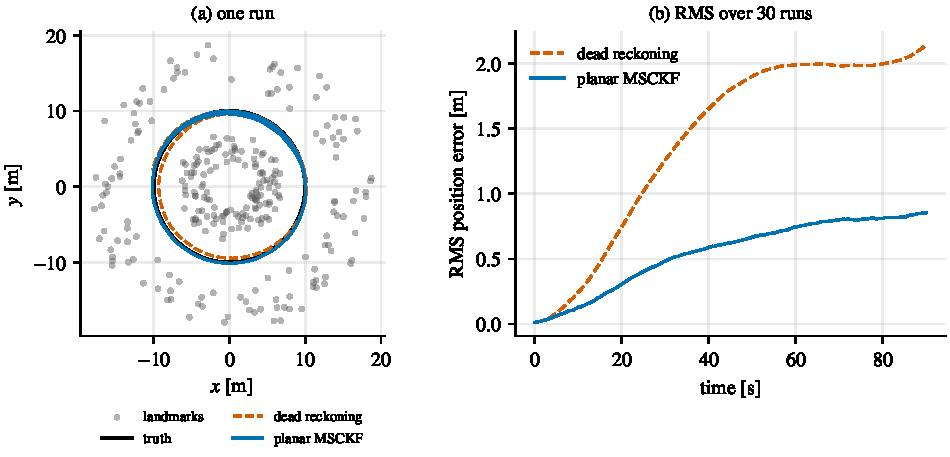
\includegraphics[width=\linewidth]{fig_planar_traj.pdf}
\caption{Planar MSCKF versus dead reckoning. (a) One run. (b) Root-mean-square position error over 30 Monte Carlo runs: after
\SI{90}{s}, \SI{0.85}{m} for the MSCKF against \SI{2.1}{m} for odometry alone.}
\label{fig:planar-traj}
\end{figure}

\begin{figure}[t]
\centering
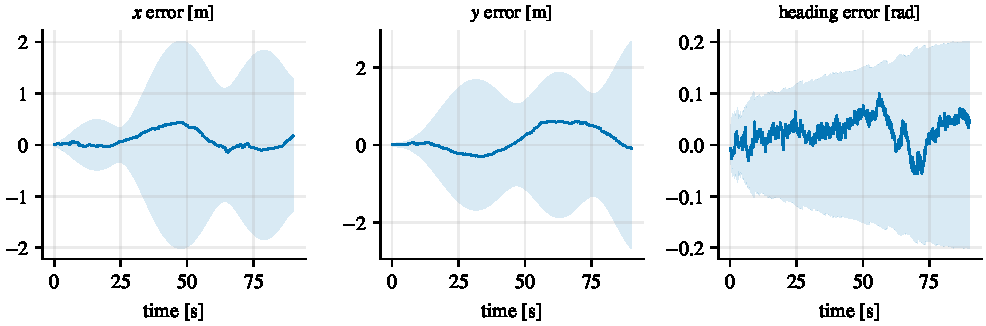
\includegraphics[width=\linewidth]{fig_planar_err.pdf}
\caption{Estimation errors of one run with the filter's $\pm3\sigma$ envelopes (shaded). The position envelopes oscillate because most of the position
uncertainty is perpendicular to the direction of travel, which rotates as the robot circles.}
\label{fig:planar-err}
\end{figure}

\begin{figure}[t]
\centering
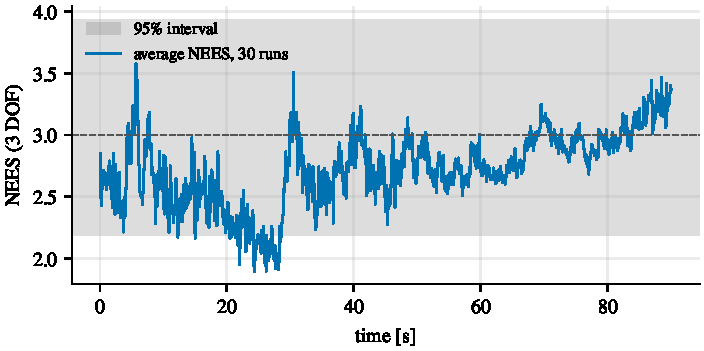
\includegraphics[width=0.8\linewidth]{fig_planar_nees.pdf}
\caption{Average NEES of the robot pose over 30 runs, with the 95\% acceptance interval of \cref{eq:anees-bounds}.}
\label{fig:planar-nees}
\end{figure}

The results (\cref{fig:planar-traj,fig:planar-err,fig:planar-nees}) illustrate four points.
\begin{enumerate}
  \item \textbf{The camera helps, mostly through the heading.} Odometry alone accumulates a heading error with standard deviation
        $\sigma_\omega\sqrt{t} = \SI{0.19}{rad}$ after \SI{90}{s}. The MSCKF ends at about \SI{0.07}{rad}: the camera measures the relative rotation between clones far
        better than the gyro-like turn rate, and because heading errors turn into cross-track position errors, the position error drops by a
        factor of 2.5.
  \item \textbf{The error still grows.} Even with the camera, the heading and position uncertainties grow without bound (\cref{fig:planar-err}).
        This is not a failure: global position and heading are unobservable (\cref{sec:planar-unobservable}), and an odometry filter without loop
        closures can only slow their drift, never stop it. The along-track error is set by the odometry speed noise alone, since a monocular camera
        cannot measure scale (the worked example above).
  \item \textbf{The filter is consistent.} The errors stay inside their $3\sigma$ envelopes, and the average NEES stays inside its acceptance
        interval, apart from mildly conservative dips below it between about 12 and \SI{28}{s}. The gate rejected 5.2\% of the features, close to the 5\% that a $\chi^2_{0.95}$ gate should reject when the filter is
        consistent and every feature is a good one; a much larger rate would signal an overconfident filter or bad data.
  \item \textbf{But the NEES creeps upward.} In the second half of the run its 15-second averages rise steadily, from 2.75 to 2.86 to 3.05, with peaks near 3.5. It is still inside the
        interval, but the trend is systematic: the filter is beginning to believe it knows the heading better than it does. The mechanism, and its cure, are the subject of \cref{ch:observability}.
\end{enumerate}

% ------------------------------------------------------------------------------
\section{The unobservable directions}
\label{sec:planar-unobservable}
\index{unobservable directions!planar}

Suppose we rotate the entire world, the trajectory and every feature, about the origin by a small angle, or translate it. Odometry measures
speed and turn rate in the body frame and does not notice. The camera measures bearings relative to the robot and does not notice either. No
sensor can therefore distinguish the true world from the rotated or translated one: these three directions are \emph{unobservable}
(\cref{sec:observability-linear}), and the filter should never gain information along them.

In error-state coordinates the three directions are the columns of
\begin{equation}
  N = \begin{bmatrix} N_t & N_r \end{bmatrix}, \qquad
  N_t = \begin{bmatrix} I_2 \\ 0 \\ I_2 \\ 0 \\ \vdots \end{bmatrix}, \qquad
  N_r = \begin{bmatrix} \Omega\hat p \\ 1 \\ \Omega\hat p_1 \\ 1 \\ \vdots \end{bmatrix},
  \label{eq:planar-nullspace}
\end{equation}
with one block pair for the robot and one for each clone. $N_t$ shifts every position by the same vector. $N_r$ is the derivative of a rotation
about the origin: a point $p$ moves by $\delta\,\Omega p$, and every heading increases by $\delta$.

\begin{proposition}[The planar nullspace]
\label{prop:planar-nullspace}
If all Jacobians are evaluated at one common set of estimates, then:
\begin{enumerate}
  \item every feature Jacobian satisfies $H_{x,j}N_t + H_{f,j} = 0$ and $H_{x,j}N_r + H_{f,j}\,\Omega\hat p_f = 0$, and therefore the projected Jacobian
        satisfies $H_{o,j}N = 0$;
  \item the exact transition \eqref{eq:planar-phi} maps the nullspace at step $k$ to the nullspace at step $k+1$, $\Phi_kN(\hat x_k) = N(\hat x_{k+1})$;
  \item cloning maps $N$ to the nullspace of the augmented state, $JN = N_{\text{aug}}$.
\end{enumerate}
\end{proposition}
\begin{proof}
(1) Row $i$, translation: $-J_\pi R_i\T + J_\pi R_i\T = 0$. Rotation: using $R_i\T\Omega = \Omega R_i\T$ (\cref{lem:omega}(3)),
\begin{equation*}
  -J_\pi R_i\T\Omega\hat p_i - J_\pi\Omega\hat p_{b,i} + J_\pi R_i\T\Omega\hat p_f = J_\pi\big(\Omega R_i\T(\hat p_f - \hat p_i) - \Omega\hat p_{b,i}\big) = J_\pi(\Omega\hat p_{b,i} - \Omega\hat p_{b,i}) = 0 .
\end{equation*}
Multiplying by $A_j\T$ and using $A_j\T H_{f,j} = 0$ gives $A_j\T H_{x,j}N = 0$.
(2) On the robot block, $\Phi_k(I_2, 0) = (I_2, 0)$, and $\Phi_k(\Omega\hat p_k, 1) = (\Omega\hat p_k + \Omega(\hat p_{k+1} - \hat p_k), 1) = (\Omega\hat p_{k+1}, 1)$; clone blocks are untouched.
(3) The new clone copies the robot's rows of $N$, which are exactly the rows a clone at $\hat p$ should have.
\end{proof}

In words: the linearized filter has the same three unobservable directions as the real system, \emph{as long as every Jacobian uses the same
estimate of each quantity}. A real filter cannot honour this condition. The transition $\Phi_k$ uses $\hat p_{k+1} - \hat p_k$ computed from the
estimate before the update at step $k+1$, while the next transition starts from the corrected estimate; and a clone is linearized at its
current, corrected estimate, not at the value it had when it was created. The identities of \cref{prop:planar-nullspace} then hold only
approximately, the linearized system has an observable heading that the real system does not, and the filter slowly gains spurious heading
information. That is the upward creep in \cref{fig:planar-nees}. \Cref{ch:observability} analyses it in the planar EKF-SLAM setting, where it is most
visible, and shows how First-Estimates Jacobians restore the nullspace.

% ------------------------------------------------------------------------------
\section{From the plane to three dimensions}
\label{sec:planar-to-3d}

\Cref{tab:planar-to-3d} lists every difference between the planar filter and the project's filter. None of them changes the structure of
\cref{alg:planar-msckf}; each changes a formula inside it.

\begin{table}[t]
\centering
\small
\caption{The planar MSCKF and its three-dimensional counterpart.}
\label{tab:planar-to-3d}
\begin{tabularx}{\linewidth}{@{}>{\raggedright\arraybackslash}p{0.2\linewidth}>{\raggedright\arraybackslash}X>{\raggedright\arraybackslash}X@{}}
\toprule
& Plane & Project (AGENTS.md) \\
\midrule
Attitude & heading $\psi$, $R(\psi) = \exp(\psi\Omega)$ & $q_{wb}$, $R_{wb}$, $\Exp$ (\cref{ch:lie}) \\
Error and retraction & $\delta\psi = \psi - \hat\psi$; local and global coincide & local (right) perturbation $q = \hat q\otimes\Exp_q(\delta\theta)$ (C4) \\
Skew operator & $\Omega$, commutes with every $R(\psi)$ & $\sx{\cdot}$; $R\sx{v}R\T = \sx{Rv}$, no commutation \\
Jacobian of $R\T a$ w.r.t.\ the rotation error & $-\Omega R\T a$ & the inverse-action row of \cref{tab:jacobians} \\
Motion sensor & odometry $(v, \omega)$, no biases & IMU $(a_m, \omega_m)$ with gravity and biases (C6) \\
State & $(p, \psi)$ + clones, $3 + 3N$ & $(p, v, q, b_a, b_g)$ + clones, $15 + 6N$ (C3) \\
Camera & 1D bearing $z = y/x$ & 2D normalized $(x/z, y/z)$, through $T_{bc}$ (C6) \\
Constraints per feature & $M - 2$ & $2M - 3$ \\
Reset Jacobian & $1$ & $I - \tfrac12\sx{\delta\hat\theta}$ per attitude (F4) \\
Unobservable directions & 2 translations + heading & 3 translations + yaw (roll and pitch are observable through gravity) \\
\bottomrule
\end{tabularx}
\end{table}

\begin{takeaways}
\begin{itemize}
  \item In the plane every MSCKF Jacobian takes a line: $\partial z/\partial\delta\psi_i = -(1 + z^2)$, $\partial z/\partial\delta p_i = -J_\pi R_i\T$, $H_f = J_\pi R_i\T$.
  \item A camera measures rotation independently of depth, and translation only through parallax ($1/x$).
  \item A feature seen $M$ times gives $M - 2$ constraints in the plane ($2M - 3$ in space); for three views the constraint is a second difference
        that measures the ratio of baselines and the relative headings, but not scale, global position or global heading.
  \item The planar filter is consistent and reduces the dead-reckoning error by a factor of about 2.5, yet its NEES creeps upward: the first sign
        of the spurious heading information studied in \cref{ch:observability}.
  \item The step to three dimensions changes formulas, not structure: non-commuting rotations, the local perturbation, gravity, biases and the reset Jacobian.
\end{itemize}
\end{takeaways}

\begin{exercises}
  \item Verify \cref{prop:planar-H} by finite differences at a random clone pose and feature. Then explain $\partial z/\partial\delta\psi = -(1 + z^2)$ using
        only the bearing angle $\beta = \arctan z$.
  \item Show that $I + F_c\Dt$ and the exact $\Phi_k$ of \eqref{eq:planar-phi} differ by $O(\Dt^2)$, and identify the term.
  \item Add a turn-rate bias $b_\omega$ ($\omega_m = \omega + b_\omega + n_\omega$, $\dot b_\omega = n_b$) to the planar state. Derive the new column of $F_c$ and the new
        row of $G_c$, and show that the bias is observable once the camera sees features. Compare with the gyroscope-bias block of the
        three-dimensional filter.
  \item Repeat the worked example with unequal baselines, $\hat p_3 = (0, 2)$. Find $a$, and show that the projected residual measures the
        ratio of the two baselines.
  \item In the worked example, show that moving the \emph{middle} clone along the viewing direction $x_w$ is invisible to $H_o$, while moving the
        \emph{first} clone along $x_w$ is visible. Interpret the difference in terms of the bearing each clone has to the feature.
  \item Why does a 1D camera need three views of a feature to say anything about the poses, while a 2D camera needs only two? Relate the answer
        to the dimensions of $H_f$.
  \item Run \code{scripts/planar\_sims.py} with window sizes $N_{\max} = 3, 5, 10, 20$ and plot the final RMS position error. Explain the trend, and what
        limits the benefit of a longer window.
  \item Prove part (1) of \cref{prop:planar-nullspace} without using the closed-form Jacobians: argue directly that a measurement function that depends only
        on $R(\psi_i)\T(p_f - p_i)$ cannot change under a common rotation or translation of all positions.
  \item Replace the bearing camera by a range-and-bearing sensor. How many constraints does a feature seen $M$ times give? Which of the unobservable
        directions of \eqref{eq:planar-nullspace} become observable, if any?
\end{exercises}
% Solutions to the exercises of Chapter 27.
\begin{solutions}
  \item At a random clone pose and a feature with $\hat z = 0.3$, central differences with $\varepsilon = 10^{-6}$ agree with \eqref{eq:planar-H} to $10^{-10}$ in all five entries. For the
        heading entry, $\beta = \arctan z$ is the angle between the body axis $x_b$ and the ray to the feature. Turning the robot left by $\delta\psi$ turns the body axis
        toward the ray, so every bearing \emph{decreases} by exactly $\delta\psi$, whatever the depth: $\delta\beta = -\delta\psi$. Since $z = \tan\beta$,
        \[
          \frac{\partial z}{\partial\delta\psi} = \frac{\dd z}{\dd\beta}\,\frac{\partial\beta}{\partial\delta\psi} = \frac{1}{\cos^2\beta}\,(-1) = -(1 + \tan^2\beta) = -(1 + z^2).
        \]
        The factor $1 + z^2$ only converts angle to normalized coordinate: at the edge of the $\pm50^\circ$ field of view it is $2.4$, while in angle every point moves
        by the same $\delta\psi$.

  \item The top-right block of $I + F_c\Dt$ is $\Omega R(\hat\psi_k)e_1v_m\Dt$, while that of $\Phi_k$ is $\Omega(\hat p_{k+1} - \hat p_k) = \Omega R(\hat\psi_k + \tfrac12\omega_m\Dt)e_1v_m\Dt$. With
        $R(\hat\psi_k + \tfrac12\omega_m\Dt) = R(\hat\psi_k)(I + \tfrac12\omega_m\Dt\,\Omega) + O(\Dt^2)$ and $\Omega^2 = -I$,
        \[
          \Phi_k - (I + F_c\Dt) = \begin{bmatrix} 0 & -\tfrac12v_m\omega_m\Dt^2\,R(\hat\psi_k)e_1 \\ 0 & 0\end{bmatrix} + O(\Dt^3).
        \]
        The term is $\tfrac12\Dt^2\,\Omega\ddot{\hat p}$: the nominal path turns during the step, so its displacement is not $\dot{\hat p}_k\Dt$. Note that $F_c^2 = 0$, so for a
        \emph{constant} $F_c$ the matrix exponential would add nothing. The whole difference comes from $F_c$ changing during the step: $I + F_c\Dt$ is the rectangle rule for
        $I + \int F_c\,\dd t$. For the simulation ($v = 1$~m/s, $\omega = 0.1$~rad/s, $\Dt = 0.01$~s) it is $5\times10^{-6}$ per step, relative size $\tfrac12\omega\Dt = 5\times10^{-4}$. It is small,
        but it means the approximate transitions no longer telescope exactly into $\Omega(\hat p_k - \hat p_0)$ (\cref{ch:observability}).

  \item With $\omega = \omega_m - b_\omega - n_\omega$ and the nominal $\dot{\hat\psi} = \omega_m - \hat b_\omega$, $\dot{\delta\psi} = -\delta b_\omega - n_\omega$ and $\dot{\delta b}_\omega = n_b$; the position row is unchanged. For
        $\delta x_R = (\delta p, \delta\psi, \delta b_\omega)$ and $n = (n_v, n_\omega, n_b)$,
        \[
          F_c = \begin{bmatrix} 0_{2\times2} & \Omega R(\hat\psi)e_1v_m & 0_{2\times1} \\ 0 & 0 & -1 \\ 0 & 0 & 0 \end{bmatrix}, \qquad
          G_c = \begin{bmatrix} -R(\hat\psi)e_1 & 0 & 0 \\ 0 & -1 & 0 \\ 0 & 0 & 1 \end{bmatrix},
        \]
        with $Q_c = \diag(\sigma_v^2, \sigma_\omega^2, \sigma_b^2)$: the new column of $F_c$ is $(0, 0, -1, 0)\T$ and the new row of $G_c$ is $(0, 0, 1)$. The camera measures relative headings of
        the clones directly: the heading column $-(1 + z^2)$ does not depend on depth, and turning a single clone is visible. A bias error makes the heading error grow
        linearly across the window, $\delta\psi(t) = \delta\psi_0 - t\,\delta b_\omega$. The unobservable directions cannot produce such a ramp: a global rotation adds the same constant to every
        heading, and translations and scale leave headings unchanged. So the ramp changes the projected residuals, and the bias is observable. Numerically: on
        the simulated circle with ten clones and six landmarks, the observability matrix of $(\delta p, \delta\psi, \delta b_\omega)$ at the first clone time has rank one. Its
        three-dimensional nullspace (the two translations and the rotation) has bias components of $10^{-14}$.
        \ifsolutions
        In three dimensions the attitude row is $\dot{\delta\theta} = -\sx{\hat\omega}\delta\theta - \delta b_g - n_g$ and the bias row $\dot{\delta b}_g = n_{b_g}$. The $-I$ in the gyro-bias columns is the exact
        counterpart of the $-1$ here. The extra term $-\sx{\hat\omega}\delta\theta$ has no planar analog, because a planar heading error does not rotate with the body. For the same
        reason as here, all three gyroscope-bias components are observable once the camera measures relative attitudes: even the bias about the vertical,
        although the global yaw is not.
        \else
        In three dimensions the same mechanism makes all three gyroscope-bias components observable once the camera measures relative attitudes: even the bias
        about the vertical, although the global yaw is not. (The corresponding block of $F_c$ is part of the derivation exercises of \cref{ch:errordyn}.)
        \fi

  \item The body-frame points are $(4, 1)$, $(4, 0)$, $(4, -2)$, so $\hat z = (\tfrac14, 0, -\tfrac12)$ and
        \[
          H_f = \begin{bmatrix} -\tfrac1{16} & \tfrac14 \\ 0 & \tfrac14 \\ \tfrac18 & \tfrac14 \end{bmatrix}, \qquad
          h_1\times h_2 = \tfrac1{64}(-2, 3, -1), \qquad a = \tfrac1{\sqrt{14}}(2, -3, 1),
        \]
        so $r_o = (2r_1 - 3r_2 + r_3)/\sqrt{14}$. For sideways motion at a fixed heading, $z_i = (y_f - y_i)/x_f$ is a linear function of the camera position $y_i = (-1, 0, 2)$, and
        the weights annihilate exactly the constants and the linear functions: $\sum_ia_i = 0$ and $\sum_ia_iy_i = 0$. For baselines $b_1 = y_2 - y_1$ and $b_2 = y_3 - y_2$, the weights are
        $(b_2, -(b_1 + b_2), b_1)$, and $r_o = 0$ exactly when
        \[
          \frac{z_1 - z_2}{z_2 - z_3} = \frac{b_1}{b_2} .
        \]
        The depth $x_f$ cancels in the ratio of image displacements, so the residual compares the observed ratio with the estimated ratio of the baselines, and
        nothing else. If the middle clone were really at $y = 0.1$, the observed ratio would be $1.1/1.9 = 0.58$ instead of $\tfrac12$, and $r_o = -0.020$. The projected Jacobian
        is $H_o = \tfrac1{\sqrt{14}}\big[(\tfrac18, -\tfrac12, -\tfrac{17}8)\ \ (0, \tfrac34, 3)\ \ (-\tfrac18, -\tfrac14, -\tfrac54)\big]$; translation, rotation and scale of the configuration give zero, as before.

  \item With $a = (1, -2, 1)/\sqrt6$, the $\delta p_x$ entries of $H_o$ are $\tfrac{1}{16\sqrt6}$, $0$ and $-\tfrac{1}{16\sqrt6}$. Moving the middle clone along $x_w$ is invisible; moving the first clone
        along $x_w$ is visible, though weakly. The middle clone looks straight at the feature ($\hat z_2 = 0$), so $x_w$ is its own viewing ray, the nullspace of its projection
        Jacobian: moving along the ray changes the depth, which one view cannot see, and leaves the bearing unchanged. The first clone sees the feature at
        $\hat z_1 = \tfrac14$ ($14^\circ$). Moving it along $x_w$ changes that bearing by $\tfrac{1}{16}$ per meter, and the feature cannot absorb the change without disturbing the other two bearings. In
        general, moving a clone along its ray to a feature is invisible in that feature's residual. Other directions are visible, with a sensitivity
        proportional to the sine of the angle between motion and ray, divided by the depth.

  \item Each observation gives as many numbers as the image has dimensions, and the feature has as many unknowns as the space. A 1D camera in the plane: $H_{f,j}$ is
        $M\times2$ of rank 2, leaving $M - 2$ constraints, so $M = 2$ gives none. Two rays in a plane always intersect (unless parallel), so any two bearings are consistent with some
        feature. A 2D camera in space: $H_{f,j}$ is $2M\times3$ of rank 3, leaving $2M - 3$, so $M = 2$ gives one. Two rays in space are generically skew, and requiring them to intersect,
        i.e.\ to be coplanar with the baseline, is the epipolar constraint (Exercise~26.3).

  \item Final RMS errors after 90~s over 30 runs (dead reckoning: $2.80$~m):
        \begin{center}\small
        \begin{tabular}{@{}l c c c c@{}}
        \toprule
        $N_{\max}$ (window length) & 3 (0.3~s) & 5 (0.5~s) & 10 (1~s) & 20 (2~s) \\
        \midrule
        position & 2.23~m & 2.13~m & 0.85~m & 0.33~m \\
        heading & 0.19~rad & 0.17~rad & 0.069~rad & 0.025~rad \\
        average NEES (last 9~s, 3 DOF) & 2.65 & 2.97 & 3.14 & 3.20 \\
        \bottomrule
        \end{tabular}
        \end{center}
        The position error follows the heading error, which turns into cross-track error. The key quantity is how well one window determines the heading
        change across it, a heading ramp, which the camera sees only through parallax. With the scenario's landmarks, a single window determines it with a
        standard deviation of $0.05$, $0.022$, $0.008$ and $0.003$~rad for $N_{\max} = 3$, 5, 10, 20. Odometry alone has $\sigma_\omega\sqrt T = 0.009$, $0.013$, $0.019$ and $0.028$~rad over the same spans.
        Short windows are worse than odometry at exactly the quantity that drives the drift; the camera wins only for windows longer than about half a second,
        which is where the error drops. The benefit then levels off: $0.18$~m at $N_{\max} = 40$ and $0.17$~m at 80. Several things limit it:
        \begin{itemize}
          \item once the window pins the heading change far better than odometry, the remaining error is the unobservable drift of global heading and
                position, which no window removes;
          \item tracks end (here a landmark stays in view for a median of 6.8~s), so a longer window cannot lengthen them;
          \item the cost grows as $n^3$ with $n = 3 + 3N_{\max}$;
          \item old clones are never relinearized;
          \item the NEES creeps upward ($3.24$ at $N_{\max} = 80$), as more constraints feed more spurious heading information (\cref{ch:observability}).
        \end{itemize}

  \item Let $h(x, p_f) = \pi\big(R(\psi_i)\T(p_f - p_i)\big)$, or any function of $R(\psi_i)\T(p_f - p_i)$. Translating everything by $t$ ($p_i \to p_i + t$, $p_f \to p_f + t$) leaves $p_f - p_i$ unchanged.
        Rotating everything about the origin by $\delta$ ($p_i \to R(\delta)p_i$, $\psi_i \to \psi_i + \delta$, $p_f \to R(\delta)p_f$) gives
        $R(\psi_i + \delta)\T R(\delta)(p_f - p_i) = R(\psi_i)\T R(\delta)\T R(\delta)(p_f - p_i) = R(\psi_i)\T(p_f - p_i)$. So $h$ is constant along both families, identically in $t$ and $\delta$.
        Differentiating at $t = 0$ and $\delta = 0$, at the common linearization point $(\hat x, \hat p_f)$: the state moves along $N_t$ and the feature by $I$, or the state along $N_r$ and the
        feature by $\Omega\hat p_f$. Hence
        \[
          H_{x,j}N_t + H_{f,j} = 0, \qquad H_{x,j}N_r + H_{f,j}\,\Omega\hat p_f = 0,
        \]
        and multiplying by $A_j\T$ gives $H_{o,j}N = 0$. Nothing about $\pi$ was used. The proof also shows why the hypothesis matters: the identities come from differentiating one
        function at one point, so they hold only if every block of $H_{x,j}$ and $H_{f,j}$ is evaluated at the same estimates.

  \item Each observation $(\|d_i\|, \atantwo(d_y, d_x))$ now gives two numbers for two unknowns of the feature, so a feature seen $M$ times gives $2M - 2$ constraints. A single
        observation determines the feature and constrains nothing; two observations already give two constraints. None of the directions of
        \eqref{eq:planar-nullspace} becomes observable: the measurement is still a function of $R(\psi_i)\T(p_f - p_i)$ alone, so the argument of Exercise~8 applies unchanged, and global
        translation and heading remain invisible. What changes is scale. The range measures distances, so the shape \emph{and size} of the trajectory are now
        observable from the camera alone, and the along-track error no longer depends on the odometry speed noise only.
\end{solutions}


\chapter{The Complete Algorithm}
\label{ch:fullalgo}

\begin{objectives}
\begin{itemize}
  \item Assemble every component into one event-driven estimator, with the correct order of operations.
  \item Estimate the computational budget and map the algorithm onto the project's software architecture.
  \item Diagnose the most common failures from their symptoms.
\end{itemize}
\end{objectives}

% ------------------------------------------------------------------------------
\section{The event loop}

The estimator consumes a single, time-ordered stream of sensor events. Milestone 3 builds it by merging the presorted IMU,
image (and, for testing, pose) arrays with a two-pointer merge, with the rule that an IMU sample precedes any other event
with the same timestamp. \Cref{alg:msckf} shows the loop.

\begin{algorithm}[t]
\caption{Monocular MSCKF}
\label{alg:msckf}
\begin{algorithmic}[1]
\Require event stream, calibration, noise parameters
\LineComment{load phase: allocation allowed}
\State parse data and calibration; build the event arrays; construct the filter and front end with fixed-max workspaces
\State initialize $(\hat x, P)$ (ground truth in the project, logged; static initialization otherwise)
\LineComment{streaming phase: no allocation in the core}
\For{each event $e$ in timestamp order}
  \If{$e$ is an IMU sample at $t$}
    \State propagate nominal state and covariance from $t_{prev}$ to $t$ \Comment{\cref{ch:strapdown,ch:errordyn}}
  \ElsIf{$e$ is an image at $t_c$}
    \State propagate to $t_c$ (interpolated IMU) \Comment{exact image time}
    \State front end: track, verify, undistort; update track histories \Comment{\cref{ch:frontend}}
    \State process tracks that were lost in this image \Comment{\cref{alg:msckf-update}}
    \If{$N = $ \code{kMaxClones}}
      \State process tracks with an observation at the oldest clone
      \State marginalize the oldest clone in place \Comment{\cref{ch:cloning}}
    \EndIf
    \State clone $(\hat p, \hat q)$; $P \gets JPJ\T$; attach this image's observations to the new clone
  \EndIf
  \State log state, $\diag(P)$, NIS and gate statistics to the preallocated buffer
\EndFor
\end{algorithmic}
\end{algorithm}

Three ordering rules are essential.
\begin{enumerate}
  \item \textbf{Propagate before you update.} A measurement at time $t$ must be applied to the state at time $t$, never to the
        state at the previous IMU sample.
  \item \textbf{Use a clone's observations before you delete it.} Every feature with an observation at the oldest clone is
        processed before that clone is marginalized; otherwise its information is lost.
  \item \textbf{Use each observation once.} After a track has been used, its observations are discarded. If the feature keeps
        being tracked, later observations form a new track.
\end{enumerate}
With the order of \cref{alg:msckf}, the window never holds more than \code{kMaxClones} clones, which keeps the covariance within its
fixed maximum size. A feature processed because its oldest clone is leaving cannot use the current image's observation in that
update, because the new clone does not exist yet. Implementations that clone first need room for one extra clone. Either
choice is valid; the storage bound must match it.
The planar filter of \cref{ch:planar} runs exactly this loop (\cref{alg:planar-msckf}) in a few lines of Python, which makes it a
convenient place to experiment with the ordering rules before committing to them in C++.

\begin{figure}[t]
\centering
\begin{tikzpicture}[xscale=0.9, yscale=1.0]
  \draw[->, thick] (0,0) -- (15.5,0) node[right, font=\footnotesize] {$t$};
  \foreach \x in {0,0.25,...,15.0} \draw[black!45] (\x,-0.08) -- (\x,0.08);
  \node[font=\scriptsize, black!60, below] at (0.6,-0.15) {IMU, 200 Hz};
  \foreach \k/\x in {1/1.25, 2/3.75, 3/6.25, 4/8.75, 5/11.25, 6/13.75} {
    \draw[primary, thick] (\x,-0.25) -- (\x,0.6);
    \draw[fill=primarylight, draw=primary] (\x-0.25,0.6) rectangle (\x+0.25,1.0);
    \node[font=\scriptsize] at (\x,0.8) {$C_\k$};
  }
  \node[font=\scriptsize, primary, below] at (3.75,-0.25) {image (20 Hz)};
  % features
  \draw[plotgreen, very thick] (1.25,1.35) -- (8.75,1.35) node[right, font=\scriptsize] {track $f_1$ lost $\Rightarrow$ update};
  \fill[plotgreen] (1.25,1.35) circle (2pt) (3.75,1.35) circle (2pt) (6.25,1.35) circle (2pt) (8.75,1.35) circle (2pt);
  \draw[plotorange, very thick] (3.75,1.85) -- (13.75,1.85);
  \fill[plotorange] (3.75,1.85) circle (2pt) (6.25,1.85) circle (2pt) (8.75,1.85) circle (2pt) (11.25,1.85) circle (2pt) (13.75,1.85) circle (2pt);
  \node[font=\scriptsize, plotorange, align=left, right] at (13.85,1.95) {$f_2$: oldest clone\\leaving $\Rightarrow$ update};
  \draw[decorate, decoration={brace, amplitude=4pt}] (3.5,2.25) -- (14.0,2.25) node[midway, above=5pt, font=\scriptsize] {window (example \code{kMaxClones} = 5)};
  \draw[conv, ->] (1.25,2.5) -- (1.25,1.1) node[pos=0, above, font=\scriptsize, align=center] {$C_1$ marginalized\\when $C_6$ arrives};
\end{tikzpicture}
\caption{Timeline of the MSCKF. The IMU propagates at 200~Hz; each image creates a clone; feature tracks are processed when
they end or when the clone holding their oldest observation is about to leave the window.}
\label{fig:timeline}
\end{figure}

% ------------------------------------------------------------------------------
\section{Initialization and the first seconds}

The project initializes from ground truth, which removes the hardest failure mode from early testing and is logged as a use of
ground truth (Milestone 10b). With static initialization (\cref{ch:strapdown}), the first seconds are delicate: the yaw is
arbitrary, the accelerometer bias is entangled with tilt, and the window contains few clones with little parallax. Generous
initial covariances, and a check that enough features with sufficient parallax exist before trusting visual updates, avoid
early divergence. Inspect the IMU data of each EuRoC sequence before running on it: a static start followed by vigorous
motion is the easiest case for initialization, and a fast start the hardest.

% ------------------------------------------------------------------------------
\section{Computational budget}

With $N = 10$ clones the error state has $n = 75$ dimensions. Rough flop counts per operation:
\begin{center}\small
\begin{tabular}{@{}l l r@{}}
\toprule
Operation & Frequency & Cost (flops) \\
\midrule
Nominal propagation & 200 Hz & $\sim10^2$ \\
$P_{II}$, $P_{IC}$ propagation & 200 Hz & $\sim4\times10^4$ \\
Cloning ($P \gets JPJ\T$ as block copies) & 20 Hz & $\sim10^4$ \\
Per feature: triangulation, projection, gating ($M = 6$) & per track & $\sim10^5$ \\
QR compression of $d = 450$ rows & per update & $\sim5\times10^6$ \\
Update ($S$, gain, Joseph) with $n = 75$ & per update & $\sim6\times10^6$ \\
Front end (KLT on 150 features) & 20 Hz & dominant in time \\
\bottomrule
\end{tabular}
\end{center}
The filter core needs on the order of $10^7$ flops per image, a few milliseconds on an embedded processor and well under a
millisecond on a desktop. The front end is usually the bottleneck in wall-clock time. The cubic growth with $n$ is why the window
is short and why QR compression matters for large stacks.

% ------------------------------------------------------------------------------
\section{Software architecture}

\begin{figure}[t]
\centering
\begin{tikzpicture}[node distance=8mm and 10mm]
  \node[block, minimum width=48mm, align=left] (core) {\textbf{vio\_core} (static, Eigen only)\\ \footnotesize so3, imu\_integrator, es\_ekf,\\ \footnotesize camera\_model, triangulation, msckf\_update};
  \node[block, minimum width=34mm, above left=10mm and -14mm of core, align=left] (io) {\textbf{vio\_io}\\ \footnotesize dataset\_loader, telemetry\\ \footnotesize + YAML parser};
  \node[block, minimum width=34mm, above right=10mm and -14mm of core, align=left] (fe) {\textbf{vio\_frontend}\\ \footnotesize visual\_frontend\\ \footnotesize + OpenCV};
  \node[block, minimum width=30mm, above=24mm of core, fill=white] (app) {\textbf{vio\_app}\\ \footnotesize main.cpp};
  \draw[->, thick] (io) -- (core); \draw[->, thick] (fe) -- (core);
  \draw[->, thick] (app) -- (io); \draw[->, thick] (app) -- (fe); \draw[->, thick] (app) -- (core);
  \node[font=\footnotesize, align=center, below=2mm of core] {arrows: ``depends on''. OpenCV never reaches \code{vio\_core};\\ each test links only the library it tests.};
\end{tikzpicture}
\caption{Library targets of the project (AGENTS.md). Dependencies point one way, so the estimator core can be built, tested and
reasoned about without the I/O and vision libraries.}
\label{fig:architecture}
\end{figure}

\Cref{fig:architecture} shows how the algorithm maps to the project's targets. The zero-allocation discipline applies to
\code{vio\_core}, which contains everything executed per IMU sample and per update. The front end may allocate but must reuse its
buffers, and the I/O layer allocates freely during loading.

% ------------------------------------------------------------------------------
\section{Debugging guide}

\begin{table}[t]
\centering\small
\begin{tabularx}{\textwidth}{@{}>{\raggedright\arraybackslash}p{4.4cm} X@{}}
\toprule
\textbf{Symptom} & \textbf{Likely causes} \\
\midrule
Altitude diverges at about $2g$ in IMU-only propagation & gravity or specific-force sign; $g_w$ added twice \\
Position diverges within seconds even with ground-truth init & $R_{wb}$ used as $R_{bw}$; quaternion $w/z$ swapped at load; gyro and accel columns or biases swapped; degrees vs radians \\
Rotation matrices slowly scale vectors & missing quaternion normalization \\
NaN after a while & missing Taylor branch; $\Log$ near $\pi$; $\Jrinv$ evaluated beyond $\pi$; feature at zero depth; Cholesky of a non-PD $S$ \\
Corrections systematically make things worse & sign of $H$ or of the residual; injection on the wrong side of the quaternion; global vs local convention mixed \\
Covariance loses symmetry or positive definiteness & simple update form instead of Joseph; missing symmetrization; aliasing in Eigen block products \\
Nearly all features fail the gate & overconfident $P$; $T_{bc}$ inverted; pixel noise used in normalized units (or vice versa); distortion not removed; timestamps misaligned \\
Gate rejects nothing & $R_z$ or $\sigma_{uv}$ far too large; gate threshold indexed with the wrong dimension \\
Slowly growing yaw error with healthy NIS & expected EKF inconsistency along unobservable yaw (\cref{ch:observability}) \\
Scale drift & little acceleration (degenerate motion); accelerometer noise or bias badly tuned \\
Works on synthetic data, fails on EuRoC & extrinsics, time offset, distortion, noise inflation, initialization, IMU gaps \\
Results differ between runs & uninitialized memory (run the sanitizers); unseeded random generators \\
\bottomrule
\end{tabularx}
\caption{Symptoms and their most frequent causes.}
\label{tab:debugging}
\end{table}

\Cref{tab:debugging} collects the failures that experience shows are most common. The milestone structure of the project is itself
the most effective debugging tool: each layer is verified against known truth before the next is built on top of it, so a new
failure is almost always in the newest layer.

\section{What to expect on EuRoC}

Published monocular filter-based estimators reach absolute trajectory errors of the order of 0.1 to 0.5~m on the machine-hall
sequences, depending on features, tuning and initialization, with the difficult sequences (fast motion, motion blur, dark
regions) considerably worse~\cite{delmerico2018benchmark}. Milestone 10b sets a first-pass target of 0.5~m on MH\_01 and a stretch target of
0.2~m. Yaw and position drift without bound; roll and pitch remain accurate throughout; velocity and biases converge within the
first seconds of excitation.

\begin{takeaways}
\begin{itemize}
  \item One time-ordered stream; propagate to each event's time before applying it.
  \item At each image: process lost tracks; if the window is full, process the oldest clone's tracks and marginalize it; then clone.
  \item The core costs about $10^7$ flops per image; the front end usually dominates the run time.
  \item Dependencies point one way: \code{vio\_core} knows nothing about files, YAML or OpenCV.
  \item Most failures map to a small set of sign, frame, unit and timing errors; test each layer against truth.
\end{itemize}
\end{takeaways}

\begin{exercises}
  \item Write the event-loop pseudocode for the alternative ordering (clone first, then process and marginalize). What capacity
        does it require, and what does it gain?
  \item Instrument a run to record the number of features processed per update, their observation counts, and the stacked row
        count $d$. Choose the compile-time row cap from the distribution.
  \item For each row of \cref{tab:debugging}, design a unit or integration test that would have caught the cause before the full
        system was assembled.
\end{exercises}
% Solutions to the exercises of Chapter 28.
\begin{solutions}
  \item With the clone created first, an image at $t_c$ is handled as follows:
        \begin{enumerate}[label=\arabic*:, leftmargin=2.2em, itemsep=0pt]
          \item propagate to $t_c$; run the front end;
          \item clone $(\hat p, \hat q)$; $P \gets JPJ\T$; attach this image's observations to the new clone (now $N + 1$ clones);
          \item process the tracks lost in this image;
          \item \textbf{if} $N + 1 > $ \code{kMaxClones}: process the tracks with an observation at the oldest clone (including the current observation), then
                marginalize the oldest clone.
        \end{enumerate}
        The window transiently holds \code{kMaxClones}$\,+\,1$ clones, so every fixed-max buffer ($P$, the stacked $H$, the clone container) must be sized for
        $15 + 6(\text{\code{kMaxClones}} + 1)$ states. The gain: a track processed because its oldest clone is leaving can include the current image's observation. That is
        its newest view and usually the one with the most parallax relative to the oldest, so it adds two rows per track and lengthens the baseline. The price
        is an update on a state six dimensions larger, about $(81/75)^3 \approx 1.26$ times the cost for \code{kMaxClones}$\,= 10$.

  \item Log, for every update, the number of features processed, each feature's $M_j$, and $d = \sum_j(2M_j - 3)$, and plot the distribution over all sequences. The
        planar filter of \cref{ch:planar} ($N_{\max} = 10$, 4\,500 updates) shows the typical shape. On average 2.4 features are processed per update. Most tracks reach the full
        window ($M = 10$ for 90\% of them), because they are processed when their oldest clone leaves. The rows per update have median 16 and 99th percentile 56,
        but the maximum is 175. The tail comes from bursts: when the window first fills, or when many features leave the view together, nearly every visible
        feature is processed at once. The worst case is therefore (visible features)$\,\times\,$(rows per full track): $150\times(2\cdot10 - 3) = 2550$ rows for the
        project. There are two sound ways to set the cap:
        \begin{itemize}
          \item size the workspace for the worst case: $2550\times76$ doubles are 1.5~MB, allocated once at load time;
          \item better, compress incrementally: append features until the next one would not fit, QR-compress the stack to $n$ rows
                (\cref{prop:compression}), and continue. The workspace then needs only $n$ plus one feature's rows ($75 + 17$), and no feature is ever dropped.
        \end{itemize}
        A cap at a percentile of the distribution without either measure would silently discard information in exactly the bursts that matter. If it is used,
        the dropped features must be counted and logged.

  \item One test per row of \cref{tab:debugging}:
        \begin{itemize}
          \item \emph{$2g$ altitude divergence:} propagate a level, stationary IMU ($a_m = (0, 0, 9.81)$, $\omega_m = 0$) for 10~s from rest; position and velocity must stay
                zero to rounding. Then propagate free fall ($a_m = 0$) and require $v_z = -9.81\,t$.
          \item \emph{Divergence within seconds:} loader tests on a fixture row with distinct values in every column (catching $w$/$z$ swaps, gyro/accel and bias column
                order, degrees). A coning test against an analytic attitude. On EuRoC, propagate IMU-only from ground truth for 1~s and compare with ground truth.
          \item \emph{Vectors slowly scaled:} after $10^6$ random multiplicative updates, $\big|\|q\| - 1\big| < 10^{-12}$.
          \item \emph{NaN:} $\Exp$, $\Log$ and $\Jrinv$ at $0$, $10^{-12}$, $\pi - 10^{-9}$ and exactly $\pi$; triangulation must reject zero and negative depths; feeding a non-PD $S$ must return an
                error, not a NaN; a randomized test asserting finite outputs.
          \item \emph{Corrections make things worse:} finite-difference tests of every Jacobian on $\bplus/\bminus$. An update with a noise-free measurement must reduce the
                error. A mutation check: flip a sign in $H$ and confirm the test fails.
          \item \emph{Covariance loses symmetry or definiteness:} after $10^4$ random updates, $\|P - P\T\| < 10^{-12}\|P\|$ and $\lambda_{\min}(P) \ge 0$. Compare in-place block products with an
                out-of-place reference.
          \item \emph{All features gated out:} a synthetic VIO run with the true noise must reject about 5\% of the features (say 3--8\%). A camera-model test projects a hand-computed
                point through $T_{bc}$ from \code{sensor.yaml}. A unit test checks $\sigma_{uv} = \sigma_{px}/f$.
          \item \emph{Gate rejects nothing:} the same run, with a lower bound on the rejection rate; the $\chi^2$ table checked against reference values, indexed by
                $\dim r$.
          \item \emph{Growing yaw error:} per-component NEES on synthetic data; position, roll and pitch must be consistent, and yaw growth is documented as expected.
          \item \emph{Scale drift:} two synthetic runs, with low and high acceleration; the scale error must be bounded in the excited run.
          \item \emph{Synthetic fine, EuRoC fails:} parse the real \code{T\_BS} (row-major) and intrinsics, and compare with hand-copied values; distortion round trip at the corners and
                edges (Exercise~20.5); merge-order test (IMU before image at equal times); IMU-gap detection ($\Dt > 2\times$ nominal flagged).
          \item \emph{Run-to-run differences:} run the pipeline twice in one test and compare outputs bitwise; sanitizers in CI; seeded generators.
        \end{itemize}
\end{solutions}



\part{Beyond the Baseline}
\chapter{Observability and Consistency of VIO}
\label{ch:observability}
\chaptermark{Observability and Consistency} % short running header

\begin{objectives}
\begin{itemize}
  \item Define observability for nonlinear systems, and test it with Lie derivatives.
  \item Prove that VIO has four unobservable directions and write them in the project's error coordinates.
  \item Show, in the planar EKF-SLAM problem where every step can be computed, exactly how the standard EKF acquires spurious information,
        and see it happen in a Monte Carlo simulation.
  \item Prove that First-Estimates Jacobians restore the correct unobservable subspace, and understand the alternatives: the
        observability-constrained EKF, the invariant EKF and robocentric formulations.
  \item Know the degenerate motions that remove further information.
\end{itemize}
\end{objectives}

The planar MSCKF of \cref{ch:planar} was consistent, but its NEES crept upward. This chapter explains the creep. The explanation needs one
new idea, observability, and one careful computation, the observability matrix of a linearized filter. The computation is done in full for
planar EKF-SLAM, the setting in which the effect was first understood~\cite{julier2001counter, bailey2006consistency, huang2010observability},
and then carried over to VIO.

% ------------------------------------------------------------------------------
\section{Observability}

\subsection{Indistinguishable states}

Consider a system $\dot x = f(x, u)$ with output $y = h(x)$. Two initial states $x_0$ and $x_0'$ are \term{indistinguishable} if, for every input
signal $u(\cdot)$, they produce the same output signal $y(\cdot)$. No estimator, however clever, can tell them apart: the data are identical. A
system is \emph{observable} at $x_0$ if no other state is indistinguishable from it. Since estimators work locally, the useful notion is
local: $x_0$ is \termi{locally weakly observable}{observability!local weak} if it can be distinguished, over arbitrarily short time intervals, from
every state in some neighborhood of it.

For linear systems the question is settled by the observability matrix (\cref{thm:obs-rank}). For a time-varying linear system
$\delta x_{k+1} = \Phi_k\delta x_k$, $r_k = H_k\delta x_k$ the same object reads as follows.

\begin{definition}[Observability matrix]
\label{def:obs-matrix}
The observability matrix over steps $1, \dots, k$ is
\begin{equation}
  \mathcal{O} = \begin{bmatrix} H_1 \\ H_2\Phi_1 \\ H_3\Phi_2\Phi_1 \\ \vdots \\ H_k\Phi_{k-1}\cdots\Phi_1 \end{bmatrix}.
\end{equation}
An initial error $\delta x_1 \in \nullsp(\mathcal{O})$ produces no change in any measurement, so it cannot be detected.
$\nullsp(\mathcal{O})$ is the \term{unobservable subspace}.
\end{definition}

A Kalman filter can gain information only in directions outside $\nullsp(\mathcal{O})$. Along unobservable directions its covariance may grow
(from process noise) but must never shrink. This is the property that the standard EKF violates.

\subsection{Nonlinear observability and Lie derivatives}

For a nonlinear system the observability matrix is replaced by derivatives of the output along the dynamics. Suppose the dynamics are
\emph{control-affine}, $\dot x = f_0(x) + \sum_i f_i(x)\,u_i$, as kinematic models usually are (the inputs are the measured rates and
accelerations). The \termi{Lie derivative}{Lie derivative} of a scalar function $\varphi$ along a vector field $f$ is its rate of change along the flow of $f$,
\begin{equation}
  L_f\varphi(x) = \nabla\varphi(x)\cdot f(x),
\end{equation}
and repeated derivatives are written $L_gL_f\varphi = \nabla(L_f\varphi)\cdot g$. Differentiating the output along a trajectory gives
\begin{equation}
  y = h(x), \qquad \dot y = L_{f_0}h + \sum_i u_i\,L_{f_i}h, \qquad \ddot y = \dots
\end{equation}
Because the inputs can be varied freely, each Lie derivative $L_{f_i}h$ is, in effect, a separate measured function of the state, and so are
the higher ones. If enough of them are available, their values pin down the state.

\begin{theorem}[Observability rank condition~\cite{hermann1977nonlinear}]
\label{thm:obs-rank-nonlinear}
Let $d\mathcal{O}(x)$ be the span of the gradients of $h$ and of all its repeated Lie derivatives $L_{f_{i_1}}\cdots L_{f_{i_m}}h$ along the vector fields of
the system. If $\dim d\mathcal{O}(x_0) = n$, the system is locally weakly observable at $x_0$.
\end{theorem}
\begin{proof}[Idea of the proof]
Choose $n$ of the functions whose gradients are independent at $x_0$ and stack them into $\Psi(x) \in \R^n$. Each is determined by the output
and the inputs (by differentiation), and $\Psi$ has an invertible Jacobian at $x_0$, so by the inverse function theorem it is one-to-one near $x_0$.
Two nearby states with the same outputs would have the same $\Psi$, hence coincide.
\end{proof}

For a linear system, $f_0 = Ax$ and $h = Cx$, the gradients are $C, CA, CA^2, \dots$: the rank condition is \cref{thm:obs-rank}. For analytic systems the
condition is also necessary in a generic sense, so a rank deficiency at typical states signals a genuine family of indistinguishable states.

\begin{worked}[a planar robot and a landmark]
A planar robot (\cref{ch:planar}) with pose $(p, \psi)$ measures the position of a landmark $\ell$ in its body frame, $h = R(\psi)\T(\ell - p) \in \R^2$. Its kinematics
are $\dot p = R(\psi)e_1\,v$ and $\dot\psi = \omega$, that is $f_v = (R(\psi)e_1, 0)$ and $f_\omega = (0, 1)$ with inputs $v$ and $\omega$.

\emph{Unknown landmark.} The state is $x = (p, \psi, \ell) \in \R^5$. With $\partial(R\T a)/\partial\psi = -\Omega R\T a$ (\cref{lem:omega}),
\begin{equation*}
  \nabla h = \begin{bmatrix} -R\T & -\Omega h & R\T \end{bmatrix}, \qquad
  L_{f_v}h = -R\T Re_1 = -e_1, \qquad L_{f_\omega}h = -\Omega h .
\end{equation*}
The first Lie derivative is constant (its gradient is zero), and $\nabla(L_{f_\omega}h) = -\Omega\nabla h$ has the same row space as $\nabla h$. Every further
derivative repeats the pattern, so $\dim d\mathcal{O} = 2$: three of the five directions are unobservable. They are the two global translations and the
global rotation, exactly the directions of \cref{sec:planar-unobservable}.

\emph{Known landmark.} If $\ell$ is known, $x = (p, \psi) \in \R^3$, the gradients are $[-R\T\ \ {-\Omega h}]$ and its multiples by $\Omega$, and the rank is 2: one
direction is unobservable. It is the rotation of the robot about the landmark, which leaves the body-frame landmark position unchanged. One known
landmark fixes position but not heading; two fix both.
\end{worked}

% ------------------------------------------------------------------------------
\section{The four unobservable directions of VIO}
\index{unobservable directions!VIO}

\begin{theorem}[Unobservable directions of VIO]
\label{thm:vio-unobservable}
For monocular VIO with point features, applying the same global translation $t$ and the same rotation $R_z(\alpha)$ about the
gravity direction to all positions, velocities, attitudes, clones and features leaves every IMU and camera measurement
unchanged. The state is therefore unobservable along these four directions.
\end{theorem}
\begin{proof}
Under $p \mapsto R_zp + t$, $v \mapsto R_zv$, $R_{wb} \mapsto R_zR_{wb}$, $p_f \mapsto R_zp_f + t$, with biases unchanged:
\begin{itemize}
  \item the gyroscope measures $\sx{\omega_b} = R_{wb}\T\dot R_{wb}$, which is invariant because $R_z$ is constant;
  \item the accelerometer measures $R_{wb}\T R_z\T(R_za_w - g_w) = R_{wb}\T(a_w - R_z\T g_w) = R_{wb}\T(a_w - g_w)$, because a rotation about
        gravity leaves $g_w$ unchanged;
  \item the camera sees $R_{bc}\T\big(R_{wb}\T R_z\T(R_zp_f + t - R_zp - t) - p_{bc}\big) = R_{bc}\T\big(R_{wb}\T(p_f - p) - p_{bc}\big)$.
\end{itemize}
All measurements are identical, so the transformed and original trajectories cannot be distinguished.
\end{proof}

Rotations about horizontal axes are \emph{not} in this family, because they would rotate gravity in the accelerometer equation;
roll and pitch are observable. Scaling is not either, because it would scale the accelerations the accelerometer measures;
scale is observable as long as the vehicle accelerates. That the remaining directions (velocity, roll, pitch, scale, biases) \emph{are}
observable under general motion is proved with the rank condition of \cref{thm:obs-rank-nonlinear}; see~\cite{hesch2014consistency} for the
computation.

Linearizing the transformation gives the unobservable directions in the project's error coordinates. With $e_z$ the vertical
unit vector, a small yaw rotation $\alpha$ and a small translation $t$ change the state by (verified numerically):
\begin{equation}
  \underbrace{\begin{bmatrix} \delta p \\ \delta v \\ \delta\theta \\ \delta b_a \\ \delta b_g \\ \delta p_i \\ \delta\theta_i \\ \delta p_f \end{bmatrix}}_{\text{error state}}
  = \underbrace{\begin{bmatrix}
    I_3 & -\sx{\hat p}\,e_z \\
    0 & -\sx{\hat v}\,e_z \\
    0 & \hat R\T e_z \\
    0 & 0 \\
    0 & 0 \\
    I_3 & -\sx{\hat p_i}\,e_z \\
    0 & \hat R_i\T e_z \\
    I_3 & -\sx{\hat p_f}\,e_z
  \end{bmatrix}}_{N}
  \begin{bmatrix} t \\ \alpha \end{bmatrix}.
  \label{eq:nullspace-N}
\end{equation}
The last row applies only to formulations that keep features in the state. The position entries follow from
$R_z(\alpha)p \approx p + \alpha\,e_z\times p = p - \alpha\sx{p}e_z$; the attitude entry is $\hat R\T e_z$ because the error is
local: $\Exp(\alpha e_z)\hat R = \hat R\,\Exp(\alpha\hat R\T e_z)$, a rotation about the world vertical expressed in body axes. Every column of $N$ \emph{depends on
the estimate}: the yaw column involves $\hat p$, $\hat v$, $\hat R$ and the clone and feature estimates. That dependence is the root of the problem.
\Cref{eq:planar-nullspace} is the planar version, with $\Omega\hat p$ in place of $-\sx{\hat p}e_z$.

% ------------------------------------------------------------------------------
\section{Why the standard EKF becomes overconfident}

If every Jacobian were evaluated at the true state, the linearized system would satisfy $\mathcal{O}N = 0$ at all times, and the
filter would never gain information along $N$. The EKF instead evaluates each Jacobian at the best estimate available when it is
computed. The transition matrix $\Phi_k$ is evaluated at the estimate after the update at step $k$, while the measurement Jacobian at step $k$ was evaluated
at the estimate before that update. The same physical state enters the observability matrix linearized at two different points, and the products
$H_k\Phi_{k-1}\cdots\Phi_1N$ no longer cancel. The planar EKF-SLAM problem shows this in a computation short enough to do completely.

\subsection{Planar EKF-SLAM}
\index{EKF-SLAM!inconsistency}\index{inconsistency!EKF}

The state is the robot pose and $L$ landmarks, $x = (p, \psi, \ell_1, \dots, \ell_L)$, with additive errors. Odometry propagates the robot
($p_{k+1} = p_k + R(\psi_k)e_1v_m\Dt$, $\psi_{k+1} = \psi_k + \omega_m\Dt$), landmarks are static, and an observation of landmark $j$ is its position in the
body frame, $z = R(\psi)\T(\ell_j - p) + n$. Writing $\hat x_{k|k-1}$ for the propagated estimate at step $k$ and $\hat x_{k|k}$ for the updated one, the EKF uses
\begin{align}
  \Phi_k &= \begin{bmatrix} I_2 & \Omega\,(\hat p_{k+1|k} - \hat p_{k|k}) \\ 0 & 1 \end{bmatrix} \oplus I_{2L}, \label{eq:slam-phi} \\
  H_k &= \begin{bmatrix} -\hat R_k\T & -\Omega\hat R_k\T(\hat\ell_j - \hat p_{k|k-1}) & 0 \cdots 0 & \hat R_k\T & 0 \cdots 0 \end{bmatrix},
  \qquad \hat R_k = R(\hat\psi_{k|k-1}), \label{eq:slam-H}
\end{align}
where $\Phi_k$ follows from \cref{prop:planar-phi} (the step starts from the updated estimate), $H_k$ from the derivation of \cref{prop:planar-H} without the
projection, and $\hat\ell_j$ is the landmark estimate at the time of the update. The candidate unobservable directions, by the argument of
\cref{sec:planar-unobservable}, are the translations $N_t = (I_2, 0, I_2, \dots, I_2)$ and the rotation
\begin{equation}
  N_r(\bar p, \bar\ell) = \big(\Omega\bar p,\ 1,\ \Omega\bar\ell_1,\ \dots,\ \Omega\bar\ell_L\big),
\end{equation}
built from some reference values $\bar p$, $\bar\ell_j$ of the positions.

\begin{theorem}[Observability of linearized planar EKF-SLAM]
\label{thm:slam-obs}
Let $\Delta_i = \hat p_{i|i} - \hat p_{i|i-1}$ be the correction of the robot position by the update at step $i$, and $D_k = \sum_{i=1}^{k-1}\Delta_i$ (with $D_1 = 0$).
For every $k$, $H_k\Phi_{k-1}\cdots\Phi_1N_t = 0$, while
\begin{equation}
  H_k\Phi_{k-1}\cdots\Phi_1\,N_r(\hat p_{1|0}, \bar\ell) = \hat R_k\T\,\Omega\,\big(D_k + \bar\ell_j - \hat\ell_j\big).
  \label{eq:slam-leak}
\end{equation}
\end{theorem}
\begin{proof}
Each $\Phi_i$ is the identity plus a term in the heading column, so the product is
$\Phi_{k-1}\cdots\Phi_1 = \begin{bmatrix} I & \Omega\,s_k \\ 0 & 1\end{bmatrix} \oplus I$ with
\begin{equation*}
  s_k = \sum_{i=1}^{k-1}\big(\hat p_{i+1|i} - \hat p_{i|i}\big)
      = \sum_{i=1}^{k-1}\big(\hat p_{i+1|i} - \hat p_{i|i-1}\big) - \sum_{i=1}^{k-1}\big(\hat p_{i|i} - \hat p_{i|i-1}\big)
      = \hat p_{k|k-1} - \hat p_{1|0} - D_k ,
\end{equation*}
since the first sum telescopes. Translations: the product leaves $N_t$ unchanged and $H_kN_t = -\hat R_k\T + \hat R_k\T = 0$. Rotation: the product
maps the robot entries $(\Omega\hat p_{1|0}, 1)$ to $(\Omega\hat p_{1|0} + \Omega s_k, 1) = (\Omega(\hat p_{k|k-1} - D_k), 1)$ and leaves the landmark entries alone, so
\begin{equation*}
  H_k(\cdot) = -\hat R_k\T\Omega(\hat p_{k|k-1} - D_k) - \Omega\hat R_k\T(\hat\ell_j - \hat p_{k|k-1}) + \hat R_k\T\Omega\bar\ell_j
  = \hat R_k\T\Omega\big(D_k + \bar\ell_j - \hat\ell_j\big),
\end{equation*}
using $\hat R_k\T\Omega = \Omega\hat R_k\T$; the $\hat p_{k|k-1}$ terms cancel.
\end{proof}

\Cref{eq:slam-leak} is the whole story. The rotation direction stays in the nullspace only if two things vanish:
\begin{itemize}
  \item $D_k$, the accumulated corrections of the robot position. They vanish only if the transition matrices telescope, which requires each $\Phi_i$
        to start where the previous one ended. The EKF starts each $\Phi_i$ from the \emph{updated} estimate $\hat p_{i|i}$, while the previous one ended at the
        \emph{propagated} estimate $\hat p_{i|i-1}$.
  \item $\bar\ell_j - \hat\ell_j$, the change of the landmark estimate between its linearization points. A single fixed reference $\bar\ell_j$ cannot match an
        estimate that every update moves.
\end{itemize}
For generic estimates no other choice of reference values makes \eqref{eq:slam-leak} vanish for all $k$, and the unobservable subspace of the EKF's
linearized model shrinks from three dimensions to two~\cite{huang2010observability}: the heading has become observable. The filter then extracts
\emph{spurious information} about the global heading from measurements that contain none. The size of the leak is set by the size of the
corrections and of the landmark estimate changes; it is largest at loop closures, when a robot that has drifted re-observes old landmarks
and receives large corrections.

\subsection{From planar SLAM to VIO}

The same mechanism operates in VIO. The translation columns of \eqref{eq:nullspace-N} survive, because all Jacobians depend only on
\emph{differences} of positions. The yaw column does not: with estimate-dependent Jacobians $\mathcal{O}N_{\text{yaw}} \neq 0$, and the unobservable
subspace of the EKF's linearized model has dimension three instead of four~\cite{li2013msckf2, hesch2014consistency}. In the MSCKF, the
clones play the role of the landmarks: a clone is created from the propagated estimate, and every later update moves it, so its linearization
point in a measurement Jacobian differs from the one at which it entered the filter. The filter becomes overconfident in yaw, and because
yaw errors couple into position through the trajectory, its position covariance becomes too small as well. On long trajectories the NEES of
yaw and position grows steadily while the NIS can look perfectly healthy: the inconsistency lives in directions the measurements do not see
(\cref{tab:consistency-diagnosis}).

\begin{keyidea}[an inconsistency that no unit test catches]
EKF yaw inconsistency is not a bug in the usual sense: every Jacobian can pass its finite-difference test. It is a property of
linearizing at estimates that change over time. Milestone 10b therefore expects it, and asks for it to be measured and documented
rather than fixed.
\end{keyidea}

% ------------------------------------------------------------------------------
\section{First-Estimates Jacobians}
\label{sec:fej}
\index{First-Estimates Jacobians}\index{FEJ|see{First-Estimates Jacobians}}

The cure suggested by \eqref{eq:slam-leak} is to make both terms vanish by construction: evaluate every Jacobian that involves a state at the
\emph{first} estimate of that state, the value it had when it entered the filter, rather than at the latest one~\cite{huang2008fej, huang2010observability}.

\begin{proposition}[FEJ restores the nullspace]
\label{prop:fej}
In planar EKF-SLAM, evaluate the transition matrix with the propagated estimates at both ends,
\begin{equation}
  \Phi_k^{\mathrm{FEJ}} = \begin{bmatrix} I_2 & \Omega\,(\hat p_{k+1|k} - \hat p_{k|k-1}) \\ 0 & 1 \end{bmatrix} \oplus I,
\end{equation}
and the measurement Jacobian at the propagated robot estimate $\hat x_{k|k-1}$ and at the \emph{first estimate} $\hat\ell_j^{(1)}$ of each landmark. Initialize
each landmark from the propagated robot estimate, $\hat\ell_j^{(1)} = \hat p_{k|k-1} + R(\hat\psi_{k|k-1})z$, with the augmentation Jacobian evaluated there.
Then $\mathcal{O}N = 0$ for all $k$, with $N = [N_t\ \ N_r(\hat p_{1|0}, \hat\ell^{(1)})]$.
\end{proposition}
\begin{proof}
The transition matrices now telescope: $\sum_i(\hat p_{i+1|i} - \hat p_{i|i-1}) = \hat p_{k|k-1} - \hat p_{1|0}$, so $D_k$ is replaced by zero. The landmark linearization
point is fixed at $\hat\ell_j^{(1)}$, which is also the reference value in $N_r$, so $\bar\ell_j - \hat\ell_j = 0$. Both terms of \eqref{eq:slam-leak} vanish.
For a landmark initialized at step $k$, the augmentation Jacobian $[I_2\ \ \Omega R(\hat\psi_{k|k-1})z\ \ 0]$ maps the robot part of $N_r$, $(\Omega\hat p_{k|k-1}, 1)$, to
$\Omega(\hat p_{k|k-1} + R(\hat\psi_{k|k-1})z) = \Omega\hat\ell_j^{(1)}$: exactly the entry $N_r$ needs for the new landmark.
\end{proof}

Only the \emph{Jacobians} change. The residuals are still computed with the latest estimates, the mean is still propagated and updated as
before, and the filter still uses all its information. The price is that each Jacobian is evaluated slightly away from the best estimate,
which adds linearization error; when the first estimates are poor this can matter, but in practice FEJ filters are markedly more consistent and
usually more accurate.

\begin{figure}[t]
\centering
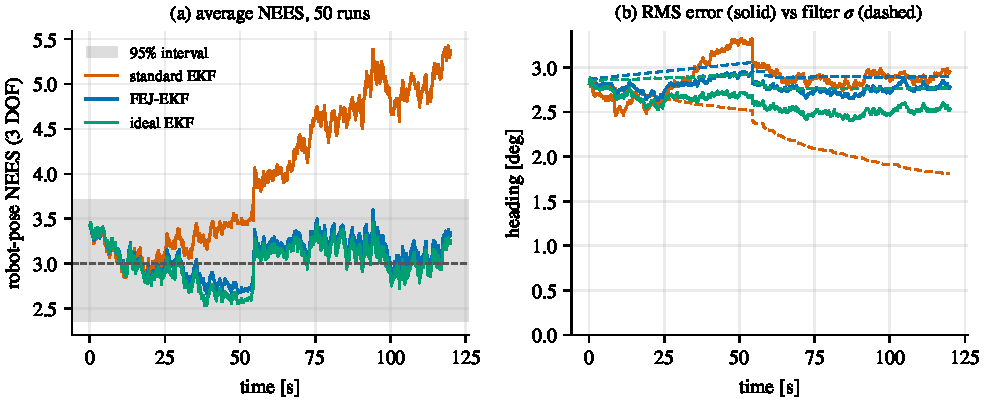
\includegraphics[width=\linewidth]{fig_fej.pdf}
\caption{Planar EKF-SLAM, 50 Monte Carlo runs. (a) Average NEES of the robot pose: the standard EKF leaves the 95\% interval after the first loop
closure (about \SI{55}{s}) and keeps rising, while the FEJ-EKF and the ideal EKF stay consistent. (b) Heading: actual RMS error (solid) and the
filter's own standard deviation (dashed). The initial heading is unobservable, so a consistent, realizable filter keeps reporting about its initial
\SI{2.9}{\degree}, as the FEJ-EKF does. The standard EKF's reported uncertainty falls to \SI{1.8}{\degree} while its actual error stays near \SI{3}{\degree}.}
\label{fig:fej}
\end{figure}

\subsection{A numerical demonstration}

\Cref{fig:fej} compares three filters on the same simulated data (\code{scripts/planar\_sims.py}). A robot drives almost twice around a circle of
radius \SI{10}{m} at \SI{1}{m/s} (\SI{120}{s}), sampling odometry at \SI{10}{Hz} (per-sample noise \SI{0.05}{m/s} in speed and \SI{0.01}{rad/s} in turn
rate), and measures the body-frame position of every landmark within \SI{5}{m} (20 landmarks are scattered around the circle), with \SI{0.1}{m} noise
per axis. The initial pose estimate has \SI{0.1}{m} position and
\SI{0.05}{rad} heading uncertainty. The three filters differ only in where they evaluate their Jacobians:
\begin{itemize}
  \item the \emph{standard EKF} uses the latest estimates, \eqref{eq:slam-phi}--\eqref{eq:slam-H};
  \item the \emph{FEJ-EKF} follows \cref{prop:fej};
  \item the \emph{ideal EKF} evaluates every Jacobian at the true state. It is not realizable, but it is the benchmark for consistency, since its
        linearized model has the true nullspace.
\end{itemize}
The heading panel makes the failure concrete. The initial heading error is unobservable, so no realizable filter can reduce it: the RMS heading
error of the standard and FEJ filters stays near its initial value of about \SI{2.9}{\degree}. (The ideal EKF reduces it slightly, to \SI{2.5}{\degree}, because
its Jacobians are evaluated at the true state, which leaks information that no real filter has.) The FEJ and ideal filters report standard
deviations that match their errors. The standard EKF reports a standard deviation that shrinks steadily, fastest at the loop closure, until its
variance is less than 40\% of its actual mean squared error. It has ``learned'' the global heading from relative measurements, which is impossible. Its NEES grows accordingly, and nothing in its
innovations reveals the problem.

\subsection{FEJ in the MSCKF}

The rule generalizes directly~\cite{li2013msckf2}: \emph{every state appears in the observability matrix at a single linearization point}. Concretely:
\begin{enumerate}
  \item \textbf{Propagation.} The transition matrix from $t_k$ to $t_{k+1}$ is evaluated with the propagated estimates at both ends,
        $\hat x_{k|k-1}$ and $\hat x_{k+1|k}$, wherever it depends on the state (positions, velocities, attitudes). The test is the planar one: the product of
        consecutive transition matrices must telescope.
  \item \textbf{Measurement.} Each clone enters the camera Jacobians at its \emph{first estimate}, the pose it had when it was cloned, not its
        current corrected value. The residual still uses the current value.
  \item \textbf{Feature.} The feature position used in $H_{x,j}$ and $H_{f,j}$ can be any single estimate (for example the triangulation from the
        current clone estimates), because the feature is eliminated: $A_j\T H_{f,j}N_f = 0$ for whatever $N_f$ the chosen value implies.
\end{enumerate}
The precise formulas depend on the error parameterization. For yours, the systematic procedure is: write $N$ in your error coordinates
(\eqref{eq:nullspace-N}), then choose the linearization points so that $\Phi_kN_k = N_{k+1}$ and $H_kN_k = 0$ hold \emph{exactly}, with $N_k$ built from the
first estimates. Even attitude blocks that do not seem to depend on the state may need attention: with a local attitude error, the yaw entry
$\hat R\T e_z$ of $N$ depends on the attitude estimate, so the attitude block of $\Phi_k$ must map $\hat R_{k|k-1}\T e_z$ to $\hat R_{k+1|k}\T e_z$.

\begin{implnote}[storing first estimates without allocation]
FEJ needs, for each clone, a second copy of its pose (the first estimate) next to the current one, and for the IMU state the propagated
estimate of the previous step. Both fit in fixed-size arrays sized by \code{kMaxClones}, so the zero-allocation rules of AGENTS.md E4 are
unaffected. A direct test: on a synthetic run, compute $\|\mathcal{O}N\|$ (or simply $\|H_kN_k\|$ and $\|\Phi_kN_k - N_{k+1}\|$ at every step) for the
standard and the FEJ filter. The FEJ values should be at rounding level, the standard ones visibly larger.
\end{implnote}

% ------------------------------------------------------------------------------
\section{Other remedies}

\subsection{Observability-constrained EKF}
\index{observability-constrained EKF}

Instead of choosing linearization points, the observability-constrained EKF (OC-EKF)~\cite{hesch2014consistency} computes Jacobians at
the latest estimates and then modifies them minimally so that the nullspace conditions hold.

\begin{proposition}[Minimal Jacobian corrections]
\label{prop:oc-ekf}
Let $N_k$ have full column rank. The matrix closest to $H$ in the Frobenius norm that satisfies $H^*N_k = 0$ is
\begin{equation}
  H^* = H\big(I - N_k(N_k\T N_k)\inv N_k\T\big),
\end{equation}
and the matrix closest to $\Phi$ that satisfies $\Phi^*N_k = N_{k+1}$ is
\begin{equation}
  \Phi^* = \Phi + (N_{k+1} - \Phi N_k)(N_k\T N_k)\inv N_k\T .
\end{equation}
\end{proposition}
\begin{proof}
The Frobenius norm is the sum of the squared norms of the rows, and the constraints act on each row separately: row $h$ must satisfy
$h^*N_k = c$ for a given row vector $c$ ($c = 0$ for $H$, a row of $N_{k+1}$ for $\Phi$). Minimizing $\|h^* - h\|^2$ subject to $h^*N_k = c$ is a least-norm problem
for the correction $d = h^* - h$: $dN_k = c - hN_k$. Its minimum-norm solution is $d = (c - hN_k)(N_k\T N_k)\inv N_k\T$ (\cref{sec:least-squares}), which gives both
formulas.
\end{proof}

The OC-EKF thus projects the information along $N$ out of every measurement and enforces the correct propagation of $N$, so the linearized
model has the correct unobservable subspace by construction. The choice of $N_k$ (which estimates to build it from) still matters; Hesch et
al.\ build it from the propagated estimates.

\subsection{Invariant EKF}
\index{invariant EKF}\index{extended pose group}

The invariant EKF~\cite{barrau2017invariant} attacks the root cause: the estimate dependence of $N$. It represents the IMU state as one element
of the \emph{extended pose group} $\mathrm{SE}_2(3)$,
\begin{equation}
  X = \begin{bmatrix} R & v & p \\ 0 & 1 & 0 \\ 0 & 0 & 1 \end{bmatrix} \in \R^{5\times5}, \qquad
  X\inv = \begin{bmatrix} R\T & -R\T v & -R\T p \\ 0 & 1 & 0 \\ 0 & 0 & 1 \end{bmatrix},
\end{equation}
a generalization of $\SE$ (\cref{sec:se3}) with two translation-like columns (features can be appended as further columns), and it defines the
error as the \emph{right-invariant} group error $\eta = \hat XX\inv = \Exp(\xi)$, with $\xi = (\xi_R, \xi_v, \xi_p) \in \R^9$.

\begin{proposition}[Constant unobservable directions]
\label{prop:invariant-nullspace}
In right-invariant error coordinates, the four unobservable directions of \cref{thm:vio-unobservable} are the constant vectors
$\xi = (e_z, 0, 0)$ (yaw) and $\xi = (0, 0, t)$, $t \in \R^3$ (translation), independent of the estimate.
\end{proposition}
\begin{proof}
A global yaw and translation act on the true state from the left: $X \mapsto GX$ with $G = \begin{bmatrix} R_z & 0 & t \\ 0 & 1 & 0 \\ 0 & 0 & 1\end{bmatrix}$, which is
$p \mapsto R_zp + t$, $v \mapsto R_zv$, $R \mapsto R_zR$. The error becomes $\hat X(GX)\inv = \hat XX\inv G\inv = \eta\,G\inv$. For small errors and a small
$G = \Exp(\epsilon)$, with $\epsilon = (\alpha e_z, 0, t)$, the product $\Exp(\xi)\Exp(-\epsilon)$ is $\Exp(\xi - \epsilon)$ to first order. The family of
indistinguishable states therefore differs, in error coordinates, by the constant vectors $\epsilon$.
\end{proof}

Compare \eqref{eq:nullspace-N}, where the yaw direction involves $\hat p$, $\hat v$ and $\hat R$. Because the group structure couples rotation with velocity
and position, a global yaw is a pure rotation error in these coordinates. Two consequences follow. The linearized error dynamics of the IMU (without
biases) are independent of the estimate, $\dot\xi = A\xi + \dots$ with
$A = \begin{bmatrix} 0 & 0 & 0 \\ \sx{g_w} & 0 & 0 \\ 0 & I & 0 \end{bmatrix}$, and $AN = 0$ because $\sx{g_w}e_z = 0$; and since every measurement is invariant under
$X \mapsto GX$, every measurement Jacobian, evaluated at \emph{any} estimate, annihilates the constant $N$. The linearized filter has the correct
unobservable subspace by construction, with no bookkeeping of first estimates. Biases break the exact estimate-independence of the error dynamics,
but not this nullspace property, since $N$ has no bias components. The price is a different state representation, different Jacobians, and a different reset;
it is a deviation from AGENTS.md C3--C4 that this project does not take.

\subsection{Robocentric formulations}
\index{robocentric filter}

A robocentric filter expresses everything relative to the current body frame, so the unobservable global quantities are not estimated at all,
and the global pose is recovered by composing relative motions outside the filter. The nullspace problem disappears with the unobservable states,
at the cost of a more complex propagation in which every state moves when the body moves.

\begin{center}\small
\begin{tabularx}{\linewidth}{@{}l>{\raggedright\arraybackslash}X>{\raggedright\arraybackslash}X@{}}
\toprule
Remedy & What changes & Cost \\
\midrule
FEJ & linearization points of $\Phi$ and $H$ & store first estimates; slightly larger linearization error \\
OC-EKF & Jacobians projected onto the constraint & build $N_k$ each step; extra products \\
Invariant EKF & state representation and error definition & new derivations; leaves the frozen conventions \\
Robocentric & state is relative to the body & more complex propagation \\
\bottomrule
\end{tabularx}
\end{center}

% ------------------------------------------------------------------------------
\section{Degenerate motions}
\index{degenerate motions}

\Cref{thm:vio-unobservable} assumes \emph{general} motion. Some motions remove further directions~\cite{yang2019degenerate}.
\begin{center}\small
\begin{tabular}{@{}l l@{}}
\toprule
Motion & What becomes unobservable \\
\midrule
constant velocity (no acceleration) & metric scale \\
pure rotation (no translation) & feature depths and translation scale \\
no rotation & accelerometer bias inseparable from the gravity direction (tilt) \\
at rest & both of the above, plus everything that needs parallax \\
\bottomrule
\end{tabular}
\end{center}
Each row has a short explanation. At constant velocity the accelerometer measures only gravity and bias, so nothing ties the size of the
camera's (scale-free) motion estimate to meters. Without translation there is no parallax, so depths, and with them the scale of the
translation, cannot be triangulated. Without rotation the gravity direction in the body frame is constant, and a constant error in it is
indistinguishable from a constant accelerometer bias; rotation makes gravity sweep through the body axes while the bias stays fixed, which
separates them.

The filter does not fail during such motions, provided it is consistent: its covariance simply stops shrinking along the
affected directions until informative motion returns. An inconsistent filter, by contrast, may ``learn'' these quantities from
noise. When a vehicle is known to be stationary, a \emph{zero-velocity update} (the pseudo-measurement $v = 0$, \cref{ch:updates}) supplies real
information and stops drift, which is why many systems detect stillness explicitly.

\begin{takeaways}
\begin{itemize}
  \item The unobservable subspace is the nullspace of the observability matrix; a filter must not gain information along it. For nonlinear
        systems, the gradients of the output's Lie derivatives play the role of the observability matrix.
  \item VIO has four unobservable directions: global translation and rotation about gravity. Roll, pitch and scale are observable
        under general motion.
  \item In local error coordinates the yaw direction is $\hat R\T e_z$ for the attitude and $-\sx{\hat p}e_z$ for positions: it depends on
        the estimate.
  \item Linearizing the same state at different estimates makes the global heading spuriously observable: in planar SLAM the leak is
        $\hat R_k\T\Omega(D_k + \bar\ell_j - \hat\ell_j)$, driven by the accumulated corrections and the drift of the landmark estimates.
  \item FEJ restores the nullspace by fixing each state's linearization point; OC-EKF projects the Jacobians; the invariant EKF makes the
        unobservable directions constant; degenerate motions remove further directions.
\end{itemize}
\end{takeaways}

\begin{exercises}
  \item Verify \eqref{eq:nullspace-N} numerically: apply a small yaw rotation and translation to a random state and compute
        $x'\bminus x$.
  \item Show that the translation columns of $N$ remain in the nullspace of the EKF's observability matrix even when Jacobians are
        evaluated at changing estimates.
  \item Redo the worked example on Lie derivatives with two unknown landmarks. What is the rank of $d\mathcal{O}$, and what are the unobservable
        directions?
  \item Repeat \cref{thm:slam-obs} for range-and-bearing measurements, $z = (\|d\|, \atantwo(d_y, d_x))$ with $d = R(\psi)\T(\ell_j - p)$. Show that the leak
        has the same form.
  \item Modify \code{scripts/planar\_sims.py} to print $\|H_k\Phi_{k-1}\cdots\Phi_1N\|$ for the three filters of \cref{fig:fej}, and confirm that only the
        standard EKF violates the nullspace condition.
  \item Prove that the minimum-norm solution used in \cref{prop:oc-ekf} is indeed the minimizer, by writing $d = d_\parallel + d_\perp$ with $d_\parallel$ in the row space of
        $N_k\T$.
  \item Implement a zero-velocity update as an EKF measurement and derive its $H$. When is it safe to apply?
  \item Read~\cite{li2013msckf2} and list which Jacobians must be evaluated at first estimates in the MSCKF. Sketch how you would store
        the first estimates in the project's data structures without allocation.
\end{exercises}

\chapter{Engineering a Real-Time Estimator in C++20}
\label{ch:engineering}
\chaptermark{Engineering in C++20} % short running header
\sloppy % long code identifiers cannot be hyphenated

\begin{objectives}
\begin{itemize}
  \item Know the C++ facts an estimator depends on: stack and heap, object lifetime, and the C++20 features the project uses.
  \item Understand why a real-time estimator must be deterministic, and how the project's memory tiers achieve it.
  \item Know how Eigen represents matrices, blocks and expressions, and use fixed-max-size matrices, member workspaces and
        allocation guards correctly.
  \item Avoid the Eigen pitfalls that silently corrupt numbers: dangling expression templates and aliasing.
  \item Understand what the sanitizers check and how, and how a target-based CMake build is organized.
  \item Design a test strategy in which every test can fail, and a systematic procedure for debugging a diverging filter.
\end{itemize}
\end{objectives}

The mathematics of the previous chapters is necessary but not sufficient. An estimator that is mathematically correct can still
miss its deadline because of an allocation, produce garbage because of an Eigen expression template, or pass all its tests because
the tests cannot fail. This chapter collects the engineering practices that the project encodes in AGENTS.md.

% ------------------------------------------------------------------------------
\section{C++ essentials for estimator code}
\label{sec:cpp-essentials}

\subsection{Stack, heap and object lifetime}

A C++ program keeps its data in two kinds of memory. The \term{stack} holds the local variables of the functions currently running. Entering a
function reserves a block of it by moving a pointer, and leaving the function releases the block by moving the pointer back: the cost is a
few instructions, it is the same every time, and the size of each block is fixed at compile time. The \term{heap} holds objects whose size or
lifetime is decided at run time. Obtaining heap memory (\code{new}, \code{std::vector} growth, a dynamic-size Eigen matrix) calls the memory
allocator, which must find a free block of the right size, may take a lock shared with other threads, and occasionally asks the operating
system for more pages. Its cost is usually modest and occasionally large, which is exactly what a real-time loop cannot afford.

Every C++ object has a lifetime that ends at a precisely defined point: a local variable when its scope closes, a member when its owner is
destroyed. At that point its destructor runs. Tying resources (memory, files, locks) to object lifetime is called \term{RAII} (resource
acquisition is initialization): a \code{std::vector} frees its heap block in its destructor, so it cannot leak. The project uses RAII
everywhere and never calls \code{delete} by hand. The stack is small (typically \SI{1}{MB} on Windows, \SI{8}{MB} on Linux), so large
matrices belong in class members created once, not in function locals.

\subsection{The C++20 features the project uses}

\begin{lstlisting}
inline constexpr int kImuDim = 15;   // compile-time constant, one definition

[[nodiscard]] bool update(const PoseMeasurement& z) noexcept; // result must be used
void ingest(std::span<const ImuSample> samples) noexcept;     // view of contiguous data
\end{lstlisting}

\begin{itemize}
  \item \code{constexpr} values are computed at compile time and can size arrays and Eigen matrices; \code{inline constexpr} in a header gives one
        shared definition. Dimensions, indices (AGENTS.md C3) and the $\chi^2$ table are \code{constexpr}.
  \item \code{[[nodiscard]]} makes the compiler warn (with \code{-Werror}, fail) when a caller ignores the return value: a rejected update or a failed
        factorization must not be silently dropped.
  \item \code{noexcept} promises that a function throws no exception. If one escapes anyway the program terminates, so the promise is only made
        on the hot path, where errors are reported through return values instead.
  \item \code{std::span<const T>} is a non-owning view (a pointer and a length) of contiguous elements. A function taking a span accepts an array, a
        \code{std::vector} or part of one without copying and without caring who owns the memory.
  \item \code{std::variant<A, B>} holds exactly one of several types, without heap allocation. \code{std::visit} calls the matching overload:
\end{itemize}

\begin{lstlisting}
template <class... Ts> struct Overloaded : Ts... { using Ts::operator()...; };
template <class... Ts> Overloaded(Ts...) -> Overloaded<Ts...>;

for (const SensorEvent& event : events) {           // one presorted stream
  std::visit(Overloaded{
      [&](const ImuSample& s)  { filter.propagate(s); },
      [&](const ImageEvent& e) { pipeline.on_image(e); },
  }, event);
}
\end{lstlisting}

\code{Overloaded} inherits the call operators of all the lambdas passed to it, so \code{std::visit} finds the one whose parameter type matches the
alternative currently stored. Adding a new event type to the variant without handling it is a compile error, not a silent omission.

% ------------------------------------------------------------------------------
\section{Determinism and the memory tiers}

A flight controller consumes the estimator's output at a fixed rate. A late estimate is a wrong estimate. The main source of
unpredictable latency in C++ is dynamic memory allocation: \code{new}, a \code{std::vector} that grows, a dynamic-size Eigen temporary. The
allocator may take locks, search free lists or ask the operating system for pages, with latency that is usually small and
occasionally large. The project therefore separates three tiers (AGENTS.md E4).

\begin{center}\small
\begin{tabularx}{\textwidth}{@{}l X X@{}}
\toprule
Tier & Scope & Rule \\
\midrule
Load & parsing, building event arrays, constructing the filter & allocate freely, before streaming starts \\
Core & \code{vio\_core}, per IMU sample and per update & zero heap allocations \\
Frontend & OpenCV tracking & may allocate, must reuse buffers; allocations are measured and logged \\
\bottomrule
\end{tabularx}
\end{center}

\subsection{Fixed-max-size matrices}

The MSCKF covariance changes size as clones come and go, but never exceeds $15 + 6N_{max}$. Eigen supports exactly this case: a
matrix whose \emph{runtime} size is dynamic but whose \emph{maximum} size is a compile-time constant. Its storage is an inline array of the
maximum size, so resizing within the bound never allocates.

\begin{lstlisting}
inline constexpr int kMaxClones = 10;                  // decided in M10a
inline constexpr int kMaxDim    = 15 + 6 * kMaxClones;

using CovMatrix = Eigen::Matrix<double, Eigen::Dynamic, Eigen::Dynamic,
                                Eigen::ColMajor, kMaxDim, kMaxDim>;

CovMatrix P;          // inline storage for 75 x 75 doubles, no heap
P.resize(15, 15);     // allowed: within the compile-time maximum
\end{lstlisting}

Large workspaces ($S$, $K$, stacked $H$, temporaries for $\Phi P$) are class members, created once, rather than function-local
variables. Function-local fixed-max matrices would not allocate either, but they would live on the stack, and several of them at
once can exceed it (\cref{ch:cloning}).

\subsection{Proving it: allocation guards}

``It shouldn't allocate'' is not evidence. The project overrides the global \code{operator new} in its tests to count allocations
(\code{tests/support/alloc\_guard.hpp}), and wraps every core hot-path test with a guard that asserts a count of zero. In debug builds,
\code{EIGEN\_RUNTIME\_NO\_MALLOC} together with \code{Eigen::internal::set\_is\_malloc\_allowed(false)} makes Eigen itself abort on any internal
allocation and reports where it happened. Both mechanisms are needed, because they see different allocations. The guard sees everything that goes
through \code{operator new}: \code{std::vector} growth, \code{std::string}, \code{std::function}, \code{std::make\_unique}. Eigen, however, obtains its heap memory
directly from \code{std::malloc} through its own aligned allocator, so a dynamic \code{Eigen::MatrixXd} is invisible to the guard. Only Eigen's flag catches it,
and only in the \code{debug-sanitize} preset, where the flag is defined.

% ------------------------------------------------------------------------------
\section{Eigen in brief}
\label{sec:eigen-basics}
\index{Eigen}\index{expression templates}

\paragraph{The matrix type.} Every dense Eigen matrix is an instance of one class template,
\begin{lstlisting}
Eigen::Matrix<Scalar, Rows, Cols, Options, MaxRows, MaxCols>
\end{lstlisting}
\code{Rows} and \code{Cols} are either compile-time numbers (a \emph{fixed-size} matrix such as \code{Eigen::Matrix3d}, stored inline with no heap) or
\code{Eigen::Dynamic} (size chosen at run time, normally on the heap, such as \code{Eigen::MatrixXd}). \code{MaxRows} and \code{MaxCols} give a dynamic
matrix a compile-time upper bound, which turns its storage into an inline array: the fixed-max-size matrices used below. \code{Options} chooses the
storage order.

\paragraph{Storage order.} Memory is one-dimensional. A \emph{column-major} matrix (Eigen's default) stores column after column, so entry $(i, j)$ of
an $m\times n$ matrix lives at offset $i + jm$; a \emph{row-major} matrix stores row after row, offset $j + in$. Loops are fastest when they walk
memory contiguously, so with column-major storage the inner loop should run down a column. Mixing orders is legal but may force copies.

\paragraph{Blocks.} \code{P.block(i, j, r, c)}, \code{P.topLeftCorner(15, 15)}, \code{v.segment<3>(6)} and their relatives return \emph{views}: they refer to
the original storage, copy nothing, and can be assigned to. \code{P.block<3, 3>(6, 6) = ...} writes the attitude block of $P$ in place. The fixed-size
forms (template arguments) let Eigen unroll small operations completely.

\paragraph{Passing matrices and blocks to functions.} A parameter of type \code{const Eigen::Matrix3d\&} accepts only that exact type. To accept any
matrix or block of compatible layout, use \code{Eigen::Ref<const Eigen::MatrixXd>} (read-only) or \code{Eigen::Ref<Eigen::MatrixXd>} (writable). A
read-only \code{Ref} quietly makes a temporary copy when the argument's layout is incompatible, and for a dynamic type that copy allocates; a writable
\code{Ref} refuses to compile instead. The quiet copy is an Eigen allocation, so \code{EIGEN\_RUNTIME\_NO\_MALLOC} catches it and the
\code{operator new} guard does not.

\paragraph{Wrapping existing memory.} \code{Eigen::Map<const Eigen::Vector3d> v(ptr)} views three doubles at \code{ptr} as a vector, without copying.
It is the right tool for parsed buffers, and the wrong one for quaternions read from EuRoC: \code{Eigen::Map<Eigen::Quaterniond>} interprets memory as
$(x, y, z, w)$, while the CSV stores $(w, x, y, z)$ (AGENTS.md C2).

\paragraph{Expression templates.} \code{A + B} does not compute a matrix. It returns a small object recording ``the sum of \code{A} and \code{B}''. Only when
that object is assigned to a matrix does Eigen run a loop, and it fuses the whole expression into it: \code{D = A + B + C} is one loop with no
temporaries. Products are the exception: they are evaluated into a temporary unless told otherwise (below). This design makes Eigen fast, and it
is also the source of the \code{auto} pitfall described next.

\paragraph{Decompositions.} Linear systems are solved through decomposition objects: \code{S.llt().solve(B)} (Cholesky, for symmetric positive definite
$S$), \code{.ldlt()} (robust for semi-definite), \code{.householderQr()} and \code{.colPivHouseholderQr()} (QR, \cref{ch:numlinalg}). A decomposition object owns
a copy of the factor; for fixed-max matrices that copy is inline. \code{Eigen::LLT<Eigen::Ref<Eigen::MatrixXd>{}> llt(A)} factors \code{A} \emph{in place},
overwriting it with the factor and allocating nothing. Symmetric structure can be exploited with \code{P.selfadjointView<Eigen::Lower>()}, which reads
only one triangle.

% ------------------------------------------------------------------------------
\section{Eigen pitfalls}

\paragraph{Expression templates and \code{auto}.} Eigen operations return lightweight \emph{expression} objects that are evaluated
lazily, when they are assigned to a matrix. An expression holds the matrices it uses by reference and nested expressions by value. Storing one
with \code{auto} therefore has two dangers. If a referenced matrix is a temporary (made by \code{.eval()}, or returned by value from a function),
the reference dangles. And even if every operand still exists, the computation happens only at the later assignment, with whatever values
the operands have then.

\begin{lstlisting}
auto bad = (a + b).eval().transpose(); // refers to the temporary made by eval()
Eigen::RowVector3d x = bad;            // undefined behavior: that temporary is gone
Eigen::RowVector3d good = (a + b).transpose(); // concrete type: evaluated now

auto lazy = A * v;                     // nothing is computed here
A(0, 0) = 10.0;
Eigen::Vector3d y = lazy;              // computed now, with the modified A
\end{lstlisting}

The rule is simple: never use \code{auto} with Eigen expressions (AGENTS.md E5). Name the concrete type, or call \code{.eval()} when a
temporary really is wanted. AddressSanitizer reports the dangling case (as a use after scope), but not the stale one, which reads only valid
memory (Exercise~30.2).

\paragraph{Aliasing.} Eigen assumes that the destination of a matrix product may alias its operands and evaluates products into a
temporary. With dynamic sizes that temporary allocates. When the destination is known not to alias, \code{.noalias()} writes directly
into it. When it does alias, the temporary is required: write into a member workspace explicitly.

\begin{lstlisting}
tmp_15xN_.noalias() = Phi * P.topRightCorner(15, nc);  // reads P, writes workspace
P.topRightCorner(15, nc) = tmp_15xN_;                   // copy back
P.bottomLeftCorner(nc, 15) = tmp_15xN_.transpose();     // keep symmetry
\end{lstlisting}

Coefficient-wise operations do not alias-check. \code{A = A.transpose()} is the classic bug; use \code{A.transposeInPlace()} or symmetrize
with a workspace.

\paragraph{Passing and alignment.} Pass Eigen objects by \code{const\&} (or \code{Eigen::Ref} for blocks). Do not add
\code{EIGEN\_MAKE\_ALIGNED\_OPERATOR\_NEW}: since C++17, aligned \code{new} handles over-aligned types. The real alignment hazard is mixing
\code{-march} or alignment-changing flags between translation units or with dependencies, which the project forbids.

\paragraph{Decompositions without allocation.} Eigen's decompositions normally own their storage. Fixed-max decomposition objects held as
members, or the in-place variants that factor a matrix in its own storage, avoid per-call allocation. Whatever the API, verify with
\code{EIGEN\_RUNTIME\_NO\_MALLOC}, which sees Eigen's allocations where the \code{operator new} guard cannot.

% ------------------------------------------------------------------------------
\section{Time and events}

\begin{lstlisting}
using Clock = std::chrono::nanoseconds;
struct ImuSample   { Clock t; Eigen::Vector3d gyro, accel; };
struct ImageEvent  { Clock t; int index; };
using SensorEvent = std::variant<ImuSample, ImageEvent /*, PoseMeasurement */>;

// Delta t: subtract in integers, convert only the difference.
const double dt = std::chrono::duration<double>(t1 - t0).count();
\end{lstlisting}

Absolute time stays in 64-bit integer nanoseconds (\cref{sec:floating}). Events form one presorted sequence built at load time, so the
streaming loop is a single pass over contiguous memory, dispatched with \code{std::visit} as in \cref{sec:cpp-essentials}: no priority queue, no
allocation, no reordering surprises.

% ------------------------------------------------------------------------------
\section{Numerical robustness checklist}

\begin{itemize}
  \item Normalize every quaternion after every multiplicative update (propagation, injection, cloning).
  \item Symmetrize $P$ after propagation and after every update.
  \item Use the Joseph form; factor $S$ with Cholesky or LDL$^\mathsf{T}$; treat a failed factorization as an error to report, not to hide.
  \item Guard every $0/0$ with Taylor branches; use $\atantwo$ for angles; handle $\Log$ near $\pi$.
  \item Reject features with non-positive or tiny depth, poor parallax or large reprojection error before linearizing.
  \item Count and log gate rejections and triangulation failures.
  \item Never clamp negative eigenvalues of $P$ to hide a problem; find out why they appeared.
  \item In debug builds, assert finiteness at module boundaries so that a \code{NaN} is caught where it is born.
\end{itemize}

% ------------------------------------------------------------------------------
\section{Sanitizers}
\label{sec:sanitizers}
\index{sanitizers}\index{AddressSanitizer}\index{UndefinedBehaviorSanitizer}

C++ leaves many errors undefined: reading past the end of an array, using memory after freeing it, overflowing a signed integer. Undefined
behavior does not mean a crash; it means the compiler may assume it never happens, so the program can produce plausible wrong numbers, behave
differently between builds, or fail far from the bug. Sanitizers are compiler-inserted checks that turn these silent errors into immediate,
precise reports.
\begin{itemize}
  \item \textbf{AddressSanitizer} (ASan, \code{-fsanitize=address}) keeps a \emph{shadow memory}, one byte for every eight bytes of program memory,
        recording which bytes may be accessed. Every heap block, stack variable and global is surrounded by poisoned \emph{redzones}, and freed
        memory stays poisoned for a while. The compiler inserts a shadow check before every load and store. ASan reports heap, stack and
        global buffer overflows, use after free, use after scope and double frees, with stack traces of the access and of the allocation. The
        cost is roughly a factor of two in speed and three in memory.
  \item \textbf{UndefinedBehaviorSanitizer} (UBSan, \code{-fsanitize=undefined}) inserts checks for signed integer overflow, out-of-range shifts, integer
        division by zero, null and misaligned pointer use, invalid \code{bool} and \code{enum} values, and floating-point-to-integer conversions that
        overflow.
\end{itemize}
By default UBSan prints a message and \emph{continues}, so a test that triggers it still passes. \code{-fno-sanitize-recover=all} makes every report
abort the process, and the test preset sets \code{UBSAN\_OPTIONS=print\_stacktrace=1:halt\_on\_error=1} so the report carries a stack trace
(AGENTS.md E3). Frame pointers (\code{-fno-omit-frame-pointer}) make those traces reliable. On Windows, LeakSanitizer does not exist, so leaks are
not detected (RAII makes them rare), and an instrumented executable needs the ASan runtime DLL from \code{C:\textbackslash msys64\textbackslash clang64\textbackslash bin}
on its \code{PATH}. Sanitizers are a debug-build tool: the \code{release} preset builds without them, and both presets must pass.

% ------------------------------------------------------------------------------
\section{Modern CMake in brief}
\label{sec:cmake}
\index{CMake}

CMake describes a build as a set of \emph{targets} (libraries and executables) with properties. Modern CMake attaches every setting to a target
rather than to global variables, and lets settings propagate along the dependency graph through three keywords:
\code{PRIVATE} (used to build this target only), \code{INTERFACE} (used only by targets that link to this one) and \code{PUBLIC} (both). A library's public
include directory is \code{PUBLIC}, because its users include its headers; a warning flag is \code{PRIVATE}, because it concerns only the library's
own code.

\begin{lstlisting}
add_library(vio_warnings INTERFACE)            # carries flags, builds nothing
target_compile_options(vio_warnings INTERFACE -Wall -Wextra -Wconversion -Werror)

add_library(vio_core STATIC src/so3.cpp src/es_ekf.cpp)
target_include_directories(vio_core PUBLIC include)
target_link_libraries(vio_core PUBLIC Eigen3::Eigen PRIVATE vio_warnings)
\end{lstlisting}

The \code{vio\_warnings} target is how warnings stay off the dependencies (AGENTS.md E3): only project targets link it. Dependencies fetched with
\code{FetchContent} at a pinned tag are declared \code{SYSTEM}, so their headers are included with \code{-isystem} and do not trigger the project's warnings.
\code{CMakePresets.json} stores named configurations (generator, compiler, build type, flags, test environment), so that
\code{cmake --preset debug-sanitize}, \code{cmake --build --preset debug-sanitize} and \code{ctest --preset debug-sanitize} reproduce exactly the same build
on every machine. Catch2's \code{catch\_discover\_tests} registers each \code{TEST\_CASE} as a separate CTest test.

% ------------------------------------------------------------------------------
\section{Testing}

\begin{keyidea}[a test must be able to fail]
For every test, ask: would it still pass if I flipped the sign of X, transposed Y, or swapped two blocks? If yes, the test is
decoration. Run it once against a deliberately broken implementation to make sure it fails.
\end{keyidea}

The project's test strategy layers several kinds of evidence.
\begin{enumerate}
  \item \textbf{Algebraic unit tests}: identities such as $\Log(\Exp(\phi)) = \phi$ at zero, tiny, generic and near-$\pi$ angles.
  \item \textbf{Finite-difference Jacobian tests} built on $\bplus/\bminus$, at non-trivial states, with tolerances justified in a comment.
  \item \textbf{Closed-form trajectory tests}: synthetic trajectories with analytic IMU data and convergence-order checks.
  \item \textbf{Statistical tests}: Monte Carlo covariance checks and NEES/NIS with $\chi^2$ bounds, seeded with
        \code{std::mt19937\_64}. Because \code{std::normal\_distribution} differs between standard libraries, never hard-code values from one
        run; test statistical properties.
  \item \textbf{Invariance tests}: cloning enabled versus disabled must give identical IMU estimates when no visual updates occur.
  \item \textbf{Resource tests}: allocation guards around every core hot path.
  \item \textbf{Sanitizers}: ASan and UBSan builds with \code{-fno-sanitize-recover=all}, so that any report fails the test run
        (\cref{sec:sanitizers}).
\end{enumerate}

% ------------------------------------------------------------------------------
\section{Debugging a diverging filter}

When the full system misbehaves, resist the urge to tune. Work down the layers instead.
\begin{enumerate}
  \item Run on \textbf{synthetic data} with exactly modeled noise. If it fails there, the bug is in the code.
  \item Disable visual updates. Does IMU-only propagation from ground truth behave as \cref{fig:cov-growth} predicts, with errors
        inside $3\sigma$?
  \item Replace visual updates by \textbf{pose updates} (Milestone 6). If those are consistent, the back end is sound.
  \item Feed the MSCKF \textbf{ground-truth feature tracks} from a synthetic scene. If that works, the problem is in the front end or the
        calibration.
  \item On real data, plot each residual component over time and look for bias, oscillation or outliers.
  \item Only then adjust noise parameters, and judge the result on consistency statistics.
\end{enumerate}

\section{Going further}

Once the baseline MSCKF runs, natural extensions are First-Estimates Jacobians (\cref{ch:observability}); online calibration of the
camera-IMU extrinsics and time offset~\cite{li2013msckf2, li2014timeoffset}; stereo observations from \code{cam1}; keeping long-lived
features as SLAM landmarks; zero-velocity updates; and evaluation on the harder EuRoC sequences (V1\_03, MH\_05) and other
datasets. Each extension adds states and Jacobians, and each Jacobian gets its derivation and its finite-difference test.

\begin{takeaways}
\begin{itemize}
  \item Heap allocation has unpredictable cost; the stack is cheap but small. Large workspaces are members, created once.
  \item Determinism requires zero allocation in the core: fixed-max-size matrices, member workspaces, proven by allocation guards and
        \code{EIGEN\_RUNTIME\_NO\_MALLOC} (Eigen allocates with \code{malloc}, which the guard does not see).
  \item Never use \code{auto} with Eigen expressions; use \code{.noalias()} only when there is no aliasing.
  \item Keep time in integer nanoseconds and process one presorted event stream.
  \item Sanitizers turn undefined behavior into reports; without \code{-fno-sanitize-recover=all} UBSan reports do not fail tests.
  \item Every test must be able to fail; layer algebraic, Jacobian, closed-form, statistical and resource tests.
  \item Debug by removing layers until the failure disappears, not by tuning.
\end{itemize}
\end{takeaways}

\begin{exercises}
  \item Write a minimal allocation guard by overriding the global \code{operator new} and \code{operator delete}, and show that it detects a
        \code{std::vector::push\_back} beyond capacity but not a fixed-max Eigen \code{resize}.
  \item Construct an example in which \code{auto} with an Eigen expression produces wrong numbers without crashing. Does
        AddressSanitizer report it?
  \item Measure the time of 10\,000 covariance propagation steps with fixed-max and with fully dynamic Eigen matrices, in both build
        presets. Explain the difference.
  \item Take one of your Jacobian tests, break the Jacobian in three different ways, and record which breakages the test detects.
  \item Write a function that reads one element past the end of a \code{std::array} and another that overflows an \code{int}. Build both presets and
        record what each sanitizer reports, and what the release build does.
  \item Pass a row-major block to a function taking \code{Eigen::Ref<const Eigen::MatrixXd>} inside an allocation guard. What happens, and what
        happens if the parameter is a writable \code{Ref}?
  \item Add a third alternative to the \code{SensorEvent} variant without handling it in the \code{Overloaded} visitor. Read the compiler error.
\end{exercises}
% Solutions to the exercises of Chapter 30.
\begin{solutions}
  \item The core of a minimal guard:
\begin{lstlisting}
inline int g_allocations = 0;                  // reset before, check after
void* operator new(std::size_t n) {
  ++g_allocations;
  if (void* p = std::malloc(n)) return p;
  throw std::bad_alloc();
}
void operator delete(void* p) noexcept { std::free(p); }
void operator delete(void* p, std::size_t) noexcept { std::free(p); }
\end{lstlisting}
        Reset the counter immediately before the code under test and read it immediately after, because the test framework allocates too. Measured
        with clang/libc++:
        \begin{itemize}
          \item four \code{push\_back} calls into a vector with \code{reserve(4)}: 0 allocations; the fifth: 1 (the reallocation);
          \item resizing a fixed-max $75\times75$ matrix from $15\times15$ to $75\times75$: 0, because the storage is inline;
          \item a dynamic \code{Eigen::MatrixXd(10, 10)}: also 0. This is not because it does not allocate, but because Eigen allocates with \code{std::malloc}
                through its own aligned allocator, which never calls \code{operator new}.
        \end{itemize}
        With \code{EIGEN\_RUNTIME\_NO\_MALLOC} and \code{set\_is\_malloc\_allowed(false)}, the same \code{MatrixXd} aborts with Eigen's assertion ``heap allocation is forbidden''. The guard and
        the flag are therefore both needed. Since the flag is defined only in the \code{debug-sanitize} preset, Eigen allocations are caught only there. Defining it for the
        test targets of both presets would close that gap; it is a design decision to record in \code{PROGRESS.md}. A complete guard also overrides the aligned
        forms \code{operator new(std::size\_t, std::align\_val\_t)}, which the library implements without calling the plain one. The C++ experiments of these
        solutions are in \code{scripts/solutions/cpp}, with \code{build\_and\_run.ps1} to build and run them in both configurations.

  \item Five candidates, each assigned afterwards to a concrete type and built in both presets:
        \begin{itemize}
          \item \code{auto e = R * (a + b);} gives correct numbers in both builds. The sum is a nested expression, which Eigen stores by value, so nothing dangles.
          \item \code{auto e = (a + b).eval().transpose();} prints the right numbers in release, by luck. ASan reports \code{stack-use-after-scope}.
          \item \code{auto e = make().head<2>();}, with \code{make()} returning a \code{Vector3d} by value, behaves the same way: right by luck in release, reported by ASan.
          \item \code{auto e = (X * 2.0).eval().block(0, 0, 2, 2);} with a dynamic \code{X} prints garbage ($10^{-311}$ entries) in release without crashing.
                ASan reports \code{stack-use-after-scope}.
          \item \code{auto e = A * v;} followed by a change to \code{A} produces the product with the \emph{new} \code{A} in both builds, and no sanitizer reports anything.
        \end{itemize}
        Dangling references are undefined behavior: the optimized build may print the right numbers because
        the dead temporary's stack slot has not been reused yet, or garbage, as in the dynamic case. AddressSanitizer reports them reliably, as a read of a variable
        whose scope has ended. The stale expression is not undefined behavior at all, since every access is to valid memory. The expression is simply evaluated
        later than the reader assumed, so no sanitizer can report it. Only the rule ``no \code{auto} with Eigen'' prevents it.

  \item Ten thousand propagation steps of a $75\times75$ covariance (the $15\times15$ block with $\Phi P\Phi\T + Q$, the $15\times60$ cross block with $\Phi P_{IC}$), per step:
        \begin{center}\small
        \begin{tabular}{@{}l c c@{}}
        \toprule
        implementation & release & debug-sanitize \\
        \midrule
        fixed-max, member workspaces & \SI{3.0}{\micro\second} & \SI{500}{\micro\second} \\
        dynamic, temporaries in expressions & \SI{3.3}{\micro\second} & \SI{525}{\micro\second} \\
        dynamic, preallocated workspaces & \SI{3.3}{\micro\second} & \SI{505}{\micro\second} \\
        \bottomrule
        \end{tabular}
        \end{center}
        In release, the arithmetic (about $4\times10^4$ flops) dominates. The three small heap allocations per step of the naive dynamic version cost a few hundred
        nanoseconds, and fixed sizes let Eigen unroll the $15\times15$ parts. That gives a 10\% difference, not an order of magnitude. The dynamic version with workspaces does not allocate
        either (it ran with Eigen allocations forbidden). The case for fixed-max matrices is therefore not average speed but the \emph{guarantee}: the storage is
        inline, its bound is checked, and no forgotten \code{.noalias()} or temporary can allocate in the hot path. That is what makes the worst case predictable. The
        sanitizer build is about 170 times slower. At \code{-O0} none of Eigen's small template functions is inlined, and ASan checks every load and store. Use it to
        prove correctness (both allocation-free versions ran with \code{malloc} forbidden), never to measure speed.

  \item With the right Jacobian $\Jr$ of \cref{ch:lie}, tested against central differences of $\Log(\Exp(\phi)\T\Exp(\phi + \delta))$ ($h = 10^{-6}$, so the correct version agrees to $10^{-10}$), the
        largest error of three broken versions at four test points is:
        \begin{center}\small
        \begin{tabular}{@{}l c c c c@{}}
        \toprule
        breakage & $\phi = 0$ & $\|\phi\| = 0.05$ & $\|\phi\| = 0.5$ & $\|\phi\| = 2.5$ \\
        \midrule
        sign of the $\sx{\phi}$ term flipped (this is $\Jl$) & 0 & $4\times10^{-2}$ & $0.4$ & $1.1$ \\
        second-order term dropped & 0 & $4\times10^{-4}$ & $4\times10^{-2}$ & $0.65$ \\
        Taylor branch used below $0.1$~rad & 0 & $4\times10^{-4}$ & $8\times10^{-11}$ & $9\times10^{-11}$ \\
        \bottomrule
        \end{tabular}
        \end{center}
        A test at $\phi = 0$ detects nothing, since every version equals $I$ there. A test at a single generic angle misses the wrong branch threshold. A loose tolerance
        ($10^{-3}$, say) misses the dropped term at small angles. Hence the rules: several random points spanning the regimes (tiny, inside every branch, generic, near
        $\pi$), and a tolerance derived from the finite-difference error rather than chosen for comfort.

  \item Reading \code{a[4]} of a \code{std::array<int, 4>} and computing \code{INT\_MAX + 1}:
        \begin{itemize}
          \item \emph{release}: the read returned 1634890337 (whatever lay next on the stack) and the addition printed $-2147483648$. No crash and no message.
                Neither result is guaranteed: both are undefined behavior, and the optimizer may, for example, fold \code{x + 1 > x} to \code{true};
          \item \emph{debug-sanitize}: ASan stops at the read with \code{stack-buffer-overflow ... READ of size 4} and the file and line of the access. UBSan stops at the
                addition with \code{runtime error: signed integer overflow: 2147483647 + 1 cannot be represented in type 'int'}. With \code{-fno-sanitize-recover=all}
                both abort, so a test that triggers them fails.
        \end{itemize}
        Note that \code{std::array::operator[]} does not check bounds. ASan caught the read because the array lives on the stack between redzones. Compiling with libc++'s
        hardening (\code{-D\_LIBCPP\_HARDENING\_MODE=\_LIBCPP\_HARDENING\_MODE\_FAST}) adds a cheap bounds check that traps even in an optimized build: the process stopped with an
        illegal-instruction exception.

  \item Binding a $3\times3$ block of a row-major matrix to \code{Eigen::Ref<const Eigen::MatrixXd>} compiles and gives the right result, but \code{Ref} cannot describe a row-major block
        with column-major strides, so it copies the block into an internal \code{MatrixXd}. The operator-new guard counts 0 allocations, because the copy is an Eigen
        allocation through \code{malloc}. With \code{set\_is\_malloc\_allowed(false)} the call aborts with Eigen's assertion. A column-major block binds without any copy (it passes with
        allocations forbidden). With a writable \code{Eigen::Ref<Eigen::MatrixXd>}, the call does not compile: \code{no matching function for call to 'scale'}. A writable reference cannot
        silently redirect writes into a copy. Keep one storage order throughout the core (column-major, Eigen's default), or write the \code{Ref} type for the layout
        actually passed.

  \item With \code{PoseEvent} added to the variant and no lambda for it, libc++ stops with
\begin{lstlisting}[language={}, basicstyle=\ttfamily\footnotesize]
error: static assertion failed due to requirement
  'is_invocable_v<Overloaded<...>, const PoseEvent &>':
  std::visit requires the visitor to be exhaustive.
\end{lstlisting}
        This is followed by notes leading back to the \code{std::visit} call. Every dispatch site that forgot the new event type fails to compile, which is the point of the
        design. The one way to defeat it is a catch-all generic lambda, \code{[](const auto\&) \{\}}, which silently swallows new alternatives. Do not put one in the
        event dispatch.
\end{solutions}

\fussy


% ------------------------------------------------------------------ appendices
\appendix
\crefalias{chapter}{appendix}
\crefalias{section}{subappendix}
\part*{Appendices} % titlesec adds the TOC entry for starred parts
\chapter{Notation and Conventions}
\label{app:notation}

This appendix restates the frozen conventions of \texttt{AGENTS.md} in one place, together with the notation of these notes.

\section*{Frames and transformations}

\begin{center}\small
\begin{tabularx}{\textwidth}{@{}l l X@{}}
\toprule
Symbol & Code name & Meaning \\
\midrule
$W$ & --- & world frame: fixed, gravity-aligned, $z$ up; EuRoC \code{R} \\
$B$ & --- & body frame = IMU \code{imu0}; EuRoC \code{S} in \code{imu0} \\
$C$ & --- & left camera \code{cam0}: $z$ optical axis, $x$ right, $y$ down \\
$R_{wb}$, $q_{wb}$ & \code{R\_wb}, \code{q\_wb} & attitude, maps body to world: $v_w = R_{wb}v_b$ \\
$p_{wb}$ & \code{p\_wb} & position of $B$'s origin in $W$ \\
$v_{wb}$ & \code{v\_wb} & velocity of $B$ relative to $W$, expressed in $W$ \\
$T_{bc} = (R_{bc}, p_{bc})$ & \code{T\_bc} & camera-to-body: $p_b = R_{bc}p_c + p_{bc}$; EuRoC \code{T\_BS} of \code{cam0} \\
$g_w$ & --- & gravity, $[0, 0, -9.81]\T~\mathrm{m/s^2}$ \\
\bottomrule
\end{tabularx}
\end{center}

Naming rule: \code{<quantity>\_<to><from>}; adjacent subscripts of a product must match ($R_{wb}R_{bc} = R_{wc}$).

\section*{State, error state and noise}

\begin{center}\small
\begin{tabular}{@{}l l l@{}}
\toprule
Error index & Block & Definition \\
\midrule
0--2 & $\delta p$ & $p = \hat p + \delta p$ (world) \\
3--5 & $\delta v$ & $v = \hat v + \delta v$ (world) \\
6--8 & $\delta\theta$ & $q = \hat q\qprod\Exp_q(\delta\theta)$ (body, local) \\
9--11 & $\delta b_a$ & $b_a = \hat b_a + \delta b_a$ \\
12--14 & $\delta b_g$ & $b_g = \hat b_g + \delta b_g$ \\
$15+6i$\dots & $\delta p_i$ & clone $i$ position \\
$18+6i$\dots & $\delta\theta_i$ & clone $i$ attitude (local) \\
\bottomrule
\end{tabular}
\qquad
\begin{tabular}{@{}l l@{}}
\toprule
Noise index & Block \\
\midrule
0--2 & $n_a$ \\
3--5 & $n_g$ \\
6--8 & $n_{b_a}$ \\
9--11 & $n_{b_g}$ \\
\bottomrule
\end{tabular}
\end{center}

\section*{Operators and symbols}

\begin{center}\small
\begin{tabularx}{\textwidth}{@{}l X@{}}
\toprule
Symbol & Meaning \\
\midrule
$a\T$, $A\inv$, $A\mT$ & transpose, inverse, inverse transpose \\
$\sx{a}$, $a\hatop$ & skew-symmetric (cross-product) matrix of $a\in\R^3$ \\
$(\cdot)\veeop$ & inverse of the hat map \\
$\qprod$ & Hamilton quaternion product \\
$q^*$ & quaternion conjugate \\
$\exp$, $\log$ & matrix exponential and logarithm \\
$\Exp$, $\Log$ & $\R^3\leftrightarrow\SO$; $\Exp_q$, $\Log_q$ for unit quaternions \\
$\Jr$, $\Jl$ & right and left Jacobians of $\SO$ \\
$\bplus$, $\bminus$ & retraction and local difference (AGENTS.md C4) \\
$\hat x$, $\delta x$, $x$ & nominal (estimated), error, and true state \\
$P$, $Q_c$, $Q_d$, $R_z$ & error covariance, continuous and discrete process noise, measurement noise \\
$F_c$, $G_c$, $\Phi$ & continuous error dynamics, noise input matrix, discrete transition \\
$H$, $S$, $K$, $r$ & measurement Jacobian, innovation covariance, gain, residual \\
$\N(\mu, \Sigma)$ & Gaussian distribution \\
$\chi^2_k$, $\chi^2_p(k)$ & chi-squared distribution with $k$ DOF; its quantile at probability $p$ \\
$\pi(\cdot)$ & pinhole projection $(X/Z, Y/Z)$ \\
$u$, $\mach$ & unit roundoff $2^{-53}$, machine epsilon $2^{-52}$ \\
\bottomrule
\end{tabularx}
\end{center}

\section*{Abbreviations}

\begin{center}\small
\begin{tabularx}{\textwidth}{@{}l X@{}}
\toprule
ATE / RPE & absolute trajectory error / relative pose error \\
BCH & Baker--Campbell--Hausdorff formula \\
DOF & degrees of freedom \\
EKF / ESKF & extended / error-state Kalman filter \\
FEJ & first-estimates Jacobians \\
IMU & inertial measurement unit \\
KLT / LK & Kanade--Lucas--Tomasi tracker / Lucas--Kanade optical flow \\
MSCKF & multi-state constraint Kalman filter \\
NEES / NIS & normalized estimation error squared / normalized innovation squared \\
PSD / PD & positive semi-definite / positive definite \\
RANSAC & random sample consensus \\
SLAM & simultaneous localization and mapping \\
VIO & visual-inertial odometry \\
\bottomrule
\end{tabularx}
\end{center}

\chapter{Formula Sheet}
\label{app:formulas}

Every formula below follows the project conventions (Hamilton quaternions, local perturbations) and was verified numerically. Let
$\theta = \|\phi\|$.

\section*{Cross products}
\begin{gather*}
  \sx{a}b = a\times b = -\sx{b}a, \qquad \sx{a}\T = -\sx{a}, \qquad \sx{a}^2 = aa\T - \|a\|^2I, \qquad \sx{a}^3 = -\|a\|^2\sx{a}, \\
  \sx{a}\sx{b} = ba\T - (a\T b)I, \qquad \sx{a\times b} = \sx{a}\sx{b} - \sx{b}\sx{a}, \qquad \sx{Ra} = R\sx{a}R\T .
\end{gather*}

\section*{Exponential and logarithm}
\begin{gather*}
  \Exp(\phi) = I + \frac{\sin\theta}{\theta}\sx{\phi} + \frac{1 - \cos\theta}{\theta^2}\sx{\phi}^2, \qquad
  \Exp_q(\phi) = \Big[\cos\tfrac\theta2,\ \tfrac{\sin(\theta/2)}{\theta}\phi\Big], \\
  \theta = \atantwo\big(\tfrac12\|(R - R\T)\veeop\|,\ \tfrac12(\tr R - 1)\big), \qquad
  \Log(R) = \frac{\theta}{2\sin\theta}(R - R\T)\veeop \quad (0 < \theta < \pi), \\
  \text{near }\pi:\ uu\T = \frac{\tfrac12(R + R\T) - \cos\theta\,I}{1 - \cos\theta}, \qquad
  \Log_q(q) = 2\atantwo(\|v\|, w)\frac{v}{\|v\|}\ \text{ after } w \ge 0 .
\end{gather*}

\section*{Coefficient functions and their series}
\begin{center}\small
\begin{tabular}{@{}l l l@{}}
\toprule
Function & Closed form & Series \\
\midrule
$A(\theta)$ & $\sin\theta/\theta$ & $1 - \theta^2/6 + \theta^4/120$ \\
$B(\theta)$ & $(1 - \cos\theta)/\theta^2$ & $1/2 - \theta^2/24 + \theta^4/720$ \\
$C(\theta)$ & $(\theta - \sin\theta)/\theta^3$ & $1/6 - \theta^2/120 + \theta^4/5040$ \\
$D(\theta)$ & $1/\theta^2 - \cot(\theta/2)/(2\theta)$ & $1/12 + \theta^2/720 + \theta^4/30240$ \\
$\cos(\theta/2)$ & & $1 - \theta^2/8 + \theta^4/384$ \\
$\sin(\theta/2)/\theta$ & & $1/2 - \theta^2/48 + \theta^4/3840$ \\
$\theta/\sin\theta$ & & $1 + \theta^2/6 + 7\theta^4/360$ \\
\bottomrule
\end{tabular}
\end{center}

\section*{Jacobians of \texorpdfstring{$\SO$}{SO(3)}}
\begin{gather*}
  \Jr(\phi) = I - B\,\sx{\phi} + C\,\sx{\phi}^2, \qquad \Jrinv(\phi) = I + \tfrac12\sx{\phi} + D\,\sx{\phi}^2, \\
  \Jl(\phi) = \Jr(-\phi) = \Jr(\phi)\T = \Exp(\phi)\Jr(\phi), \qquad \Jr(\phi) = \int_0^1\Exp(-s\phi)\,\dd s, \\
  \Exp(\phi + \delta) \approx \Exp(\phi)\Exp(\Jr(\phi)\delta), \qquad
  \Log(\Exp(\phi)\Exp(\delta)) \approx \phi + \Jrinv(\phi)\delta, \\
  R\Exp(\phi)R\T = \Exp(R\phi), \qquad \Log(\Exp(a)\Exp(b)) = a + b + \tfrac12 a\times b + \cdots
\end{gather*}

\section*{Elementary Jacobians (local perturbation \texorpdfstring{$R\Exp(\delta\theta)$}{R Exp(dtheta)})}
\begin{center}\small
\begin{tabular}{@{}l l@{\qquad}l l@{}}
\toprule
$Rv$ & $-R\sx{v}$ & $R\inv$ & $-R$ \\
$R\T v$ & $\sx{R\T v}$ & $R_1R_2$ & $R_2\T$ (w.r.t.\ $R_1$), $I$ (w.r.t.\ $R_2$) \\
$\Exp(\phi)$ & $\Jr(\phi)$ & $\Log(R)$ & $\Jrinv(\Log R)$ \\
\bottomrule
\end{tabular}
\end{center}

\section*{Quaternions}
\begin{gather*}
  p\qprod q = \big[p_wq_w - p_v\T q_v,\ \ p_wq_v + q_wp_v + p_v\times q_v\big], \qquad
  R(q) = (w^2 - v\T v)I + 2vv\T + 2w\sx{v}, \\
  \dot q = \tfrac12 q\qprod[0, \omega_b], \qquad \dot R = R\sx{\omega_b}, \qquad R(p\qprod q) = R(p)R(q).
\end{gather*}

\section*{Kalman filter}
\begin{gather*}
  P \gets \Phi P\Phi\T + Q_d, \qquad \Phi \approx I + F_c\Dt, \qquad Q_d \approx G_cQ_cG_c\T\Dt, \\
  r = z\bminus h(\hat x), \quad H = \tfrac{\partial}{\partial\delta x}\big[h(\hat x\bplus\delta x)\bminus h(\hat x)\big]_0, \quad
  S = HPH\T + R_z, \quad K = PH\T S\inv, \\
  P \gets (I - KH)P(I - KH)\T + KR_zK\T, \qquad \hat x \gets \hat x\bplus Kr, \qquad P \gets GPG\T,\ G_\theta = I - \tfrac12\sx{\delta\hat\theta}.
\end{gather*}

\section*{Strapdown propagation with constant inputs (\texorpdfstring{$\phi = \hat\omega\Dt$}{phi = omega dt})}
\begin{gather*}
  R_{k+1} = R_k\Exp(\phi), \qquad v_{k+1} = v_k + g\Dt + R_k\Dt\Jl(\phi)\hat a, \\
  p_{k+1} = p_k + v_k\Dt + \tfrac12g\Dt^2 + R_k\Dt^2N(\phi)\hat a, \\
  N(\phi) = \tfrac12I + \frac{\theta - \sin\theta}{\theta^3}\sx{\phi} + \frac{\theta^2/2 + \cos\theta - 1}{\theta^4}\sx{\phi}^2 .
\end{gather*}

\section*{Noise}
\begin{gather*}
  \sigma_d = \sigma/\sqrt\Dt\ \ \text{(white, per sample)}, \qquad \sigma_{b,d} = \sigma_b\sqrt\Dt\ \ \text{(random walk, per step)}, \\
  \Var(m\text{-fold integral of white noise}) = \sigma^2\frac{t^{2m-1}}{(2m-1)((m-1)!)^2}, \\
  1\ ^\circ/\sqrt{\mathrm h} = 2.909\times10^{-4}~\mathrm{rad/s/\sqrt{Hz}} .
\end{gather*}

\section*{Geometry}
\begin{gather*}
  \bar x_2\T\sx{t}R\bar x_1 = 0, \qquad \frac{\partial\pi}{\partial p_c} = \frac1Z\begin{bmatrix} 1 & 0 & -X/Z \\ 0 & 1 & -Y/Z\end{bmatrix}, \\
  \sigma_Z \approx \sqrt2\frac{Z^2}{b}\sigma_{uv}, \qquad N_{\mathrm{RANSAC}} = \frac{\log(1-p)}{\log(1 - w^s)} .
\end{gather*}

\chapter{Statistical and Numerical Tables}
\label{app:tables}

The tables are generated by \code{scripts/make\_tables.py} with SciPy, so they can be regenerated or extended. The project's
\code{constexpr} $\chi^2$ table (AGENTS.md F3) should be generated the same way, offline, rather than typed by hand.

\section*{Quantiles of the \texorpdfstring{$\chi^2$}{chi-squared} distribution}

$\chi^2_p(k)$ is the value below which a $\chi^2_k$ variable falls with probability $p$. Gates use $\chi^2_{0.95}$ or $\chi^2_{0.99}$; two-sided
95\% intervals use $\chi^2_{0.025}$ and $\chi^2_{0.975}$. For other probability levels, rerun the script. An MSCKF feature with $M$
observations has $k = 2M - 3$.

\begin{center}
\footnotesize\setlength{\tabcolsep}{3.2pt}
\begin{tabular}{@{}rrrrrcrrrrr@{}}
\toprule
$k$ & $\chi^2_{0.025}$ & $\chi^2_{0.95}$ & $\chi^2_{0.975}$ & $\chi^2_{0.99}$ & & $k$ & $\chi^2_{0.025}$ & $\chi^2_{0.95}$ & $\chi^2_{0.975}$ & $\chi^2_{0.99}$ \\
\midrule
1 & 0.001 & 3.841 & 5.024 & 6.635 & \hspace{4pt} & 26 & 13.844 & 38.885 & 41.923 & 45.642 \\
2 & 0.051 & 5.991 & 7.378 & 9.210 & \hspace{4pt} & 27 & 14.573 & 40.113 & 43.195 & 46.963 \\
3 & 0.216 & 7.815 & 9.348 & 11.345 & \hspace{4pt} & 28 & 15.308 & 41.337 & 44.461 & 48.278 \\
4 & 0.484 & 9.488 & 11.143 & 13.277 & \hspace{4pt} & 29 & 16.047 & 42.557 & 45.722 & 49.588 \\
5 & 0.831 & 11.070 & 12.833 & 15.086 & \hspace{4pt} & 30 & 16.791 & 43.773 & 46.979 & 50.892 \\
6 & 1.237 & 12.592 & 14.449 & 16.812 & \hspace{4pt} & 31 & 17.539 & 44.985 & 48.232 & 52.191 \\
7 & 1.690 & 14.067 & 16.013 & 18.475 & \hspace{4pt} & 32 & 18.291 & 46.194 & 49.480 & 53.486 \\
8 & 2.180 & 15.507 & 17.535 & 20.090 & \hspace{4pt} & 33 & 19.047 & 47.400 & 50.725 & 54.776 \\
9 & 2.700 & 16.919 & 19.023 & 21.666 & \hspace{4pt} & 34 & 19.806 & 48.602 & 51.966 & 56.061 \\
10 & 3.247 & 18.307 & 20.483 & 23.209 & \hspace{4pt} & 35 & 20.569 & 49.802 & 53.203 & 57.342 \\
11 & 3.816 & 19.675 & 21.920 & 24.725 & \hspace{4pt} & 36 & 21.336 & 50.998 & 54.437 & 58.619 \\
12 & 4.404 & 21.026 & 23.337 & 26.217 & \hspace{4pt} & 37 & 22.106 & 52.192 & 55.668 & 59.893 \\
13 & 5.009 & 22.362 & 24.736 & 27.688 & \hspace{4pt} & 38 & 22.878 & 53.384 & 56.896 & 61.162 \\
14 & 5.629 & 23.685 & 26.119 & 29.141 & \hspace{4pt} & 39 & 23.654 & 54.572 & 58.120 & 62.428 \\
15 & 6.262 & 24.996 & 27.488 & 30.578 & \hspace{4pt} & 40 & 24.433 & 55.758 & 59.342 & 63.691 \\
16 & 6.908 & 26.296 & 28.845 & 32.000 & \hspace{4pt} & 45 & 28.366 & 61.656 & 65.410 & 69.957 \\
17 & 7.564 & 27.587 & 30.191 & 33.409 & \hspace{4pt} & 50 & 32.357 & 67.505 & 71.420 & 76.154 \\
18 & 8.231 & 28.869 & 31.526 & 34.805 & \hspace{4pt} & 60 & 40.482 & 79.082 & 83.298 & 88.379 \\
19 & 8.907 & 30.144 & 32.852 & 36.191 & \hspace{4pt} & 75 & 52.942 & 96.217 & 100.839 & 106.393 \\
20 & 9.591 & 31.410 & 34.170 & 37.566 & \hspace{4pt} & 100 & 74.222 & 124.342 & 129.561 & 135.807 \\
21 & 10.283 & 32.671 & 35.479 & 38.932 & \hspace{4pt} & 150 & 117.985 & 179.581 & 185.800 & 193.208 \\
22 & 10.982 & 33.924 & 36.781 & 40.289 & \hspace{4pt} & 200 & 162.728 & 233.994 & 241.058 & 249.445 \\
23 & 11.689 & 35.172 & 38.076 & 41.638 & \hspace{4pt} & 300 & 253.912 & 341.395 & 349.874 & 359.906 \\
24 & 12.401 & 36.415 & 39.364 & 42.980 & \hspace{4pt} & 450 & 393.118 & 500.456 & 510.670 & 522.717 \\
25 & 13.120 & 37.652 & 40.646 & 44.314 & \hspace{4pt} & 600 & 534.019 & 658.094 & 669.769 & 683.516 \\
\bottomrule
\end{tabular}

\end{center}

\section*{Average NEES acceptance intervals}

Two-sided 95\% interval $\big[\chi^2_{0.025}(Nn)/N,\ \chi^2_{0.975}(Nn)/N\big]$ for the average NEES of an $n$-dimensional error over $N$ independent
Monte Carlo runs (\cref{ch:consistency}). The same intervals apply to the time-average of $N$ independent NIS values of dimension $n$.

\begin{center}
\small\setlength{\tabcolsep}{4pt}
\begin{tabular}{@{}rcccccc@{}}
\toprule
$n \backslash N$ & 1 & 10 & 25 & 50 & 100 & 200 \\
\midrule
1 & [0.00, 5.02] & [0.32, 2.05] & [0.52, 1.63] & [0.65, 1.43] & [0.74, 1.30] & [0.81, 1.21] \\
2 & [0.05, 7.38] & [0.96, 3.42] & [1.29, 2.86] & [1.48, 2.59] & [1.63, 2.41] & [1.73, 2.29] \\
3 & [0.22, 9.35] & [1.68, 4.70] & [2.12, 4.03] & [2.36, 3.72] & [2.54, 3.50] & [2.67, 3.35] \\
6 & [1.24, 14.45] & [4.05, 8.33] & [4.72, 7.43] & [5.08, 7.00] & [5.34, 6.70] & [5.53, 6.49] \\
9 & [2.70, 19.02] & [6.56, 11.81] & [7.41, 10.74] & [7.86, 10.21] & [8.19, 9.85] & [8.42, 9.60] \\
15 & [6.26, 27.49] & [11.80, 18.58] & [12.93, 17.22] & [13.52, 16.56] & [13.95, 16.09] & [14.25, 15.77] \\
\bottomrule
\end{tabular}

\end{center}

\section*{Monte Carlo variance ratio}

If $M$ runs produce a sample variance $s^2$ of an error whose true variance is $\sigma^2$, then $s^2/\sigma^2 \sim \chi^2_{M-1}/(M-1)$. The 95\%
intervals below are the acceptance bounds for a covariance-propagation check (Milestone 5).

\begin{center}
\small\setlength{\tabcolsep}{4pt}
\begin{tabular}{@{}rcc@{}}
\toprule
runs $M$ & lower bound & upper bound \\
\midrule
50 & 0.644 & 1.433 \\
100 & 0.741 & 1.297 \\
200 & 0.813 & 1.206 \\
500 & 0.880 & 1.128 \\
1000 & 0.914 & 1.090 \\
2000 & 0.939 & 1.063 \\
\bottomrule
\end{tabular}

\end{center}

\section*{RANSAC iterations}

Number of iterations $N = \lceil\log(1 - p)/\log(1 - w^s)\rceil$ for confidence $p = 0.99$, minimal sample size $s$ and inlier ratio $w$.

\begin{center}
\small
\begin{tabular}{@{}rrrrrrrr@{}}
\toprule
$s \backslash w$ & 0.9 & 0.8 & 0.7 & 0.6 & 0.5 & 0.4 & 0.3 \\
\midrule
1 & 2 & 3 & 4 & 6 & 7 & 10 & 13 \\
2 & 3 & 5 & 7 & 11 & 17 & 27 & 49 \\
3 & 4 & 7 & 11 & 19 & 35 & 70 & 169 \\
5 & 6 & 12 & 26 & 57 & 146 & 448 & 1893 \\
7 & 8 & 20 & 54 & 163 & 588 & 2809 & 21055 \\
8 & 9 & 26 & 78 & 272 & 1177 & 7025 & 70188 \\
\bottomrule
\end{tabular}

\end{center}

\chapter{The EuRoC MAV Dataset}
\label{app:euroc}

The EuRoC MAV dataset~\cite{burri2016euroc} was recorded with an AscTec Firefly hexacopter carrying a VI-Sensor: two global-shutter
MT9V034 cameras ($752\times480$, 20~Hz) and an ADIS16448 MEMS IMU (200~Hz), hardware time-synchronized and calibrated with Kalibr.
The values below are those of the published calibration files; check them against your copy.

\section*{Directory layout}

The project keeps sequences under \code{data/<sequence>/mav0/} (git-ignored). Each sequence contains:
\begin{center}\small
\begin{tabularx}{\textwidth}{@{}l X@{}}
\toprule
Path & Content \\
\midrule
\code{imu0/data.csv} & \code{timestamp [ns], w\_x, w\_y, w\_z [rad/s], a\_x, a\_y, a\_z [m/s\textsuperscript{2}]}: $\omega_m$, $a_m$ in $B$ \\
\code{imu0/sensor.yaml} & IMU noise densities (continuous time), rate, \code{T\_BS} (identity for the IMU) \\
\code{cam0/data.csv} & \code{timestamp [ns], filename} \\
\code{cam0/data/} & PNG images named by timestamp \\
\code{cam0/sensor.yaml} & \code{T\_BS} (row-major $4\times4$), \code{intrinsics}, \code{distortion\_coefficients}, resolution, rate \\
\code{cam1/} & right camera (unused; stereo is a stretch goal) \\
\code{state\_groundtruth\_estimate0/data.csv} & \code{timestamp, p\_RS\_R (3), q\_RS (w,x,y,z), v\_RS\_R (3), b\_w\_RS\_S (3), b\_a\_RS\_S (3)} \\
\bottomrule
\end{tabularx}
\end{center}

\begin{pitfall}[ground-truth column order]
In the ground-truth file the quaternion is stored $w$ first, and the \emph{gyroscope} bias precedes the \emph{accelerometer} bias. The file
starts later than the IMU file, and its velocities and biases come from the dataset authors' own estimator that fused the
tracking-system data with the IMU, so they are reference values, not perfect truth. The project maps the columns to
$p_{wb}, q_{wb}, v_{wb}, b_g, b_a$ (AGENTS.md C7).
\end{pitfall}

\section*{IMU parameters (\texttt{imu0/sensor.yaml})}

\begin{center}\small
\begin{tabular}{@{}l l l@{}}
\toprule
Key & Value & Units \\
\midrule
\code{gyroscope\_noise\_density} & $1.6968\times10^{-4}$ & $\mathrm{rad/s/\sqrt{Hz}}$ \\
\code{gyroscope\_random\_walk} & $1.9393\times10^{-5}$ & $\mathrm{rad/s^2/\sqrt{Hz}}$ \\
\code{accelerometer\_noise\_density} & $2.0\times10^{-3}$ & $\mathrm{m/s^2/\sqrt{Hz}}$ \\
\code{accelerometer\_random\_walk} & $3.0\times10^{-3}$ & $\mathrm{m/s^3/\sqrt{Hz}}$ \\
\code{rate\_hz} & 200 & Hz \\
\bottomrule
\end{tabular}
\end{center}

\section*{Camera parameters (\texttt{cam0/sensor.yaml})}

\begin{center}\small
\begin{tabular}{@{}l l@{}}
\toprule
\code{intrinsics} $[f_u, f_v, c_u, c_v]$ & $[458.654,\ 457.296,\ 367.215,\ 248.375]$ \\
\code{distortion\_model} & \code{radial-tangential} \\
\code{distortion\_coefficients} $[k_1, k_2, p_1, p_2]$ & $[-0.28340811,\ 0.07395907,\ 0.00019359,\ 1.76187114\times10^{-5}]$ \\
\code{resolution} & $752\times480$ \\
\code{rate\_hz} & 20 \\
\bottomrule
\end{tabular}
\end{center}

The extrinsic calibration \code{T\_BS} of \code{cam0} is the project's $T_{bc}$:
\begin{equation*}
  T_{bc} \approx \begin{bmatrix}
    0.0148655 & -0.9998809 & 0.0041403 & -0.0216401 \\
    0.9995572 & 0.0149672 & 0.0257155 & -0.0646770 \\
    -0.0257744 & 0.0037562 & 0.9996607 & 0.0098107 \\
    0 & 0 & 0 & 1
  \end{bmatrix}.
\end{equation*}
Its third column shows that the optical axis $z_c$ is almost exactly the body $z$-axis, and its first two columns that the camera
$x$-axis is close to body $y$ and the camera $y$-axis close to body $-x$. The camera center sits about 7~cm from the IMU. At rest, the
EuRoC accelerometer reads close to $+g$ on its $x$-axis, so the body $x$-axis points roughly up. Verify both facts on your data: they are
exactly the kind of sanity check that catches a transposed extrinsic.

\section*{Sequences}

\begin{center}\small
\begin{tabular}{@{}l l l l@{}}
\toprule
Sequence & Environment & Difficulty & Ground truth \\
\midrule
MH\_01\_easy, MH\_02\_easy & machine hall & easy & laser tracker (position) \\
MH\_03\_medium & machine hall & medium & laser tracker (position) \\
MH\_04\_difficult, MH\_05\_difficult & machine hall & difficult (fast, dark) & laser tracker (position) \\
V1\_01\_easy, V2\_01\_easy & Vicon room & easy & motion capture (pose) \\
V1\_02\_medium, V2\_02\_medium & Vicon room & medium & motion capture (pose) \\
V1\_03\_difficult, V2\_03\_difficult & Vicon room & difficult (fast, blur) & motion capture (pose) \\
\bottomrule
\end{tabular}
\end{center}

MH\_01\_easy is the project's development sequence. The difficult sequences contain fast rotations, motion blur and poorly lit
regions; they are where robust front ends and consistent estimators make the difference.

\ifsolutions
\chapter{Solutions to the Project Derivation Exercises}
\label{app:solutions}

\begin{pitfall}[read this first]
These are the Jacobians that \texttt{AGENTS.md} (Guardrail 4) asks you to derive yourself. Attempt each exercise first, check your
result numerically, and only then compare. Every result below was verified against central finite differences built on the project's
$\bplus/\bminus$ operators.
\end{pitfall}

% ------------------------------------------------------------------------------
\section{Error-state dynamics \texorpdfstring{$F_c$}{Fc} and \texorpdfstring{$G_c$}{Gc}}
\label{sol:Fc}

\paragraph{Attitude.} Differentiate $R = \hat R\Exp(\delta\theta)$ with \cref{lem:dexp}, to first order:
\begin{equation*}
  \dot R = \dot{\hat R}\Exp(\delta\theta) + \hat R\Exp(\delta\theta)\sx{\dot{\delta\theta}}
         = \hat R\sx{\hat\omega}\Exp(\delta\theta) + \hat R\Exp(\delta\theta)\sx{\dot{\delta\theta}} .
\end{equation*}
The true kinematics give $\dot R = R\sx{\omega} = \hat R\Exp(\delta\theta)\sx{\omega}$. Equate and multiply on the left by $(\hat R\Exp(\delta\theta))\T$:
\begin{equation*}
  \sx{\omega} = \Exp(-\delta\theta)\sx{\hat\omega}\Exp(\delta\theta) + \sx{\dot{\delta\theta}} = \sx{\Exp(-\delta\theta)\hat\omega} + \sx{\dot{\delta\theta}} .
\end{equation*}
With $\Exp(-\delta\theta)\hat\omega \approx \hat\omega - \delta\theta\times\hat\omega = \hat\omega + \hat\omega\times\delta\theta$ and $\omega - \hat\omega = -\delta b_g - n_g$:
\begin{equation}
  \dot{\delta\theta} = -\sx{\hat\omega}\,\delta\theta - \delta b_g - n_g .
\end{equation}
The term $-\sx{\hat\omega}\delta\theta$, absent in the global version (\cref{ex:global-attitude}), appears because the error is expressed in body axes
that rotate with angular velocity $\hat\omega$. An error fixed in the world appears to rotate backwards in the body frame.

\paragraph{Velocity.} With $R \approx \hat R(I + \sx{\delta\theta})$ and $a_m - b_a - n_a = \hat a - \delta b_a - n_a$:
\begin{equation*}
  \dot{\hat v} + \dot{\delta v} \approx \hat R\hat a + \hat R\sx{\delta\theta}\hat a - \hat R\delta b_a - \hat Rn_a + g_w,
\end{equation*}
dropping the second-order products $\sx{\delta\theta}\delta b_a$ and $\sx{\delta\theta}n_a$. Subtracting $\dot{\hat v} = \hat R\hat a + g_w$ and using
$\sx{\delta\theta}\hat a = -\sx{\hat a}\delta\theta$:
\begin{equation}
  \dot{\delta v} = -\hat R\sx{\hat a}\,\delta\theta - \hat R\,\delta b_a - \hat R\,n_a .
\end{equation}

\paragraph{Assembly.} With the frozen orders $\delta x = [\delta p, \delta v, \delta\theta, \delta b_a, \delta b_g]$ and $w = [n_a, n_g, n_{b_a}, n_{b_g}]$:
\begin{equation}
  F_c = \begin{bmatrix}
    0 & I & 0 & 0 & 0 \\
    0 & 0 & -\hat R\sx{\hat a} & -\hat R & 0 \\
    0 & 0 & -\sx{\hat\omega} & 0 & -I \\
    0 & 0 & 0 & 0 & 0 \\
    0 & 0 & 0 & 0 & 0
  \end{bmatrix}, \qquad
  G_c = \begin{bmatrix}
    0 & 0 & 0 & 0 \\
    -\hat R & 0 & 0 & 0 \\
    0 & -I & 0 & 0 \\
    0 & 0 & I & 0 \\
    0 & 0 & 0 & I
  \end{bmatrix},
\end{equation}
all blocks $3\times3$, with $\hat R = \hat R_{wb}$, $\hat a = a_m - \hat b_a$, $\hat\omega = \omega_m - \hat b_g$. The structural zeros follow from the cascade: position
depends only on velocity; attitude does not depend on position, velocity or the accelerometer bias; the biases are driven only by
their own noise. Since $Q_c$ is block-diagonal and $\hat R\hat R\T = I$,
$Q_d \approx G_cQ_cG_c\T\Dt = \diag(0,\ \sigma_a^2I,\ \sigma_g^2I,\ \sigma_{b_a}^2I,\ \sigma_{b_g}^2I)\,\Dt$.

\paragraph{Checking the signs.} Rotating a positive error $\delta\theta$ about $\hat\omega$ itself gives $-\sx{\hat\omega}\hat\omega = 0$: an error about the rotation axis
does not move, as it should. A positive gyro bias error makes the true rate smaller than the estimated one, so the true attitude
lags and $\dot{\delta\theta} = -\delta b_g$. For a level, static IMU, $\hat a = [0, 0, g]$, and $-\sx{\hat a}\delta\theta = g\,(\delta\theta_y, -\delta\theta_x, 0)$: a tilt about $y$
produces a velocity error along $x$, the gravity leak.

% ------------------------------------------------------------------------------
\section{Closed-form blocks of \texorpdfstring{$\Phi$}{Phi}}
\label{sol:Phi}

The project's default is $\Phi \approx I + F_c\Dt$. If a higher-order transition is adopted (and logged), the exact solution of the error
dynamics over a step with constant $\hat\omega$, $\hat a$, and with $\hat R(s) = \hat R_k\Exp(\hat\omega s)$ evolving inside the step, has these blocks,
with $\phi = \hat\omega\Dt$ and $N(\phi)$ from \cref{prop:exact-prop}:
\begin{align*}
  \Phi_{\theta\theta} &= \Exp(-\phi) = \Exp(\phi)\T, & \Phi_{\theta b_g} &= -\Dt\,\Jr(\phi), \\
  \Phi_{v\theta} &= -\hat R_k\sx{\Dt\,\Jl(\phi)\hat a}, & \Phi_{vb_a} &= -\hat R_k\,\Dt\,\Jl(\phi), \\
  \Phi_{p\theta} &= -\hat R_k\sx{\Dt^2N(\phi)\hat a}, & \Phi_{pb_a} &= -\hat R_k\,\Dt^2N(\phi), \qquad \Phi_{pv} = \Dt\,I .
\end{align*}
The remaining coupling blocks ($\Phi_{vb_g}$, $\Phi_{pb_g}$) have no compact closed form; compute them by series or numerically, and use
Van Loan's method (\cref{prop:vanloan}) or a fine numerical integration of $\dot\Phi = F_c(s)\Phi$ as the test oracle. To first order in
$\Dt$, every block reduces to the corresponding block of $I + F_c\Dt$.

% ------------------------------------------------------------------------------
\section{Pose measurement Jacobian}
\label{sol:Hpose}

With $h(x) = (p_{wb}, q_{wb})$ and $r(\delta x) = h(\hat x\bplus\delta x)\bminus h(\hat x)$:
\begin{equation*}
  r_p = (\hat p + \delta p) - \hat p = \delta p, \qquad
  r_\theta = \Log_q\big(\hat q\inv\qprod\hat q\qprod\Exp_q(\delta\theta)\big) = \delta\theta .
\end{equation*}
Both are exact, so
\begin{equation}
  H = \begin{bmatrix} I_3 & 0 & 0 & 0 & 0 \\ 0 & 0 & I_3 & 0 & 0 \end{bmatrix} \in \R^{6\times15}.
\end{equation}
Its nullspace is spanned by $\delta v$, $\delta b_a$ and $\delta b_g$: these are not measured directly and are corrected through their
cross-covariances with $\delta p$ and $\delta\theta$. The simplicity of the attitude block is a consequence of the noise model
$q_{meas} = q\qprod\Exp_q(n_\theta)$ matching the local perturbation, which makes $r_\theta = \Log(\Exp(\delta\theta)\Exp(n_\theta)) \approx \delta\theta + n_\theta$.
If the residual is instead linearized around a non-zero value $r_0$ (an iterated update, or the optimization view of
\cref{sec:manifold-update}), the derivative of $\Log(\Exp(-\delta\theta)\Exp(r_0))$ with respect to $\delta\theta$ is $-\Jlinv(r_0)$, which reduces to $-I$ for small
$r_0$, the sign being that of the optimization convention.

% ------------------------------------------------------------------------------
\section{Cloning Jacobian}
\label{sol:clone}

At cloning time the true clone equals the true IMU pose and the clone's nominal equals the IMU nominal, so
\begin{equation*}
  \delta p_c = p - \hat p = \delta p, \qquad \Exp(\delta\theta_c) = \hat q\inv\qprod q = \Exp(\delta\theta)\ \Rightarrow\ \delta\theta_c = \delta\theta,
\end{equation*}
exactly, without linearization. With the new clone appended at the end of an $n = 15 + 6N$ dimensional state,
\begin{equation}
  J_g = \begin{bmatrix} I_3 & 0 & 0 & 0 & 0 & 0_{3\times6N} \\ 0 & 0 & I_3 & 0 & 0 & 0_{3\times6N} \end{bmatrix}\in\R^{6\times n},
  \qquad J = \begin{bmatrix} I_n \\ J_g \end{bmatrix}.
\end{equation}
Consequently $JPJ\T$ copies blocks: the new clone's covariance is
$\begin{bmatrix} P_{pp} & P_{p\theta} \\ P_{\theta p} & P_{\theta\theta}\end{bmatrix}$, and its cross-covariance with every other state is the stacked $p$ and $\theta$ rows of $P$.
No matrix product is needed in the implementation.

If the clone stored the camera pose, $R_{wc} = R_{wb}R_{bc}$ and $p_{wc} = p_{wb} + R_{wb}p_{bc}$ would give
$\delta\theta_c = R_{bc}\T\delta\theta$ and $\delta p_c = \delta p - \hat R\sx{p_{bc}}\delta\theta$, by the composition and rotation-action rows of \cref{tab:jacobians}. Storing the
IMU pose keeps $J$ trivial and moves the extrinsics into the measurement model.

% ------------------------------------------------------------------------------
\section{Visual measurement Jacobians}
\label{sol:Hcam}

Write $\hat d_i = \hat R_{wb_i}\T(\hat p_f - \hat p_{wb_i})$, the feature in the clone's body frame. Perturbing the clone and the feature,
\begin{equation*}
  R_{wb_i}\T(p_f - p_{wb_i}) \approx (I - \sx{\delta\theta_i})\hat R_{wb_i}\T(\hat p_f + \delta p_f - \hat p_{wb_i} - \delta p_i)
  \approx \hat d_i + \sx{\hat d_i}\delta\theta_i - \hat R_{wb_i}\T\delta p_i + \hat R_{wb_i}\T\delta p_f ,
\end{equation*}
using the inverse-action row of \cref{tab:jacobians}. Applying $R_{bc}\T$ (the subtraction of $p_{bc}$ is constant):
\begin{equation}
  \frac{\partial p_{c_i}}{\partial\delta\theta_i} = R_{bc}\T\sx{\hat d_i}, \qquad
  \frac{\partial p_{c_i}}{\partial\delta p_i} = -R_{bc}\T\hat R_{wb_i}\T, \qquad
  \frac{\partial p_{c_i}}{\partial p_f} = R_{bc}\T\hat R_{wb_i}\T .
\end{equation}
Moving the clone by $\delta$ is equivalent to moving the feature by $-\delta$, hence the opposite signs. With
$J_\pi = \frac1{\hat Z}\begin{bmatrix} I_2 & -\pi(\hat p_{c_i})\end{bmatrix}$ from \cref{prop:proj-jacobian}:
\begin{equation}
  H_{x,ji} = \Big[\ 0_{2\times15}\ \ \cdots\ \ \underbrace{-J_\pi R_{bc}\T\hat R_{wb_i}\T}_{\delta p_i}\ \ \underbrace{J_\pi R_{bc}\T\sx{\hat d_i}}_{\delta\theta_i}\ \ \cdots\ \Big],
  \qquad
  H_{f,ji} = J_\pi R_{bc}\T\hat R_{wb_i}\T ,
\end{equation}
with the two non-zero blocks in clone $i$'s columns $15 + 6i \dots 20 + 6i$, and zeros in the IMU columns and in every other clone's columns.
The stacked $H_{x,j}$ therefore has one $2\times6$ non-zero block per observation (\cref{fig:hx-sparsity}).

\paragraph{Checking the signs.} Translate the clone along the camera's optical axis toward the feature: the feature gets closer, so its
image moves away from the principal point, and $-J_\pi R_{bc}\T\hat R_{wb_i}\T\delta p_i$ predicts exactly that. Rotate the clone about the camera's
$y$-axis by a small positive angle ($\delta\theta_i = \alpha R_{bc}e_y$): the image of a distant point on the optical axis moves in $-x$, which the
$\delta\theta_i$ block reproduces (for a near point, the lever arm $p_{bc}$ adds a small translation of the camera center).

\fi

\backmatter
\chapter*{Further Reading}
\addcontentsline{toc}{chapter}{Further Reading}
\markboth{Further Reading}{}

\paragraph{Estimation theory.} Bar-Shalom, Li and Kirubarajan~\cite{barshalom2001} is the standard reference for Kalman filtering,
consistency testing (NEES, NIS) and tracking practice. Maybeck~\cite{maybeck1979} remains the clearest treatment of continuous-time
stochastic models and their discretization, and Simon~\cite{simon2006} is a modern, readable textbook.

\paragraph{Rotations and Lie theory.} Solà's quaternion notes~\cite{sola2017quaternion} derive the error-state filter with exactly the
conventions of this project and are the best single companion to \cref{ch:eskf,ch:errordyn}. The micro Lie theory
paper~\cite{sola2018micro} is a short, practical introduction to manifolds, Jacobians and $\bplus/\bminus$. Barfoot~\cite{barfoot2017state}
develops estimation on matrix Lie groups in depth. Sommer et al.~\cite{sommer2018flipped} explain the Hamilton/JPL confusion once and for all.

\paragraph{Inertial navigation.} Groves~\cite{groves2013principles} covers inertial sensors, error models and strapdown algorithms
comprehensively. El-Sheimy et al.~\cite{elsheimy2008allan} is a good introduction to the Allan variance.

\paragraph{Computer vision.} Hartley and Zisserman~\cite{hartley2004} is the reference for multi-view geometry; Ma et
al.~\cite{ma2004invitation} gives a more geometric, calibrated-camera treatment closer to how VIO uses vision. Baker and
Matthews~\cite{baker2004lk} unify the many variants of Lucas--Kanade.

\paragraph{Visual-inertial odometry.} Read the original MSCKF paper~\cite{mourikis2007msckf} first, then MSCKF 2.0~\cite{li2013msckf2}
for consistency and calibration. Huang's review~\cite{huang2019review} and Scaramuzza and Zhang~\cite{scaramuzza2019vio} survey the
field. The OpenVINS documentation and paper~\cite{geneva2020openvins} and the MSCKF-VIO code~\cite{sun2018msckfvio} are excellent
engineering references. For the optimization-based alternative, start with preintegration~\cite{forster2017preintegration}, VINS-Mono
\cite{qin2018vins} and the factor-graph tutorial of Dellaert and Kaess~\cite{dellaert2017factor}.

\paragraph{Numerical linear algebra.} Golub and Van Loan~\cite{golub2013} for factorizations, Higham~\cite{higham2002} for floating-point
error analysis.

\renewcommand{\bibname}{References}
\begin{thebibliography}{99}
\addcontentsline{toc}{chapter}{References}
\small

\bibitem{baker2004lk} S.~Baker and I.~Matthews. Lucas--Kanade 20 years on: A unifying framework. \emph{International Journal of Computer Vision}, 56(3):221--255, 2004.

\bibitem{barshalom2001} Y.~Bar-Shalom, X.~R. Li, and T.~Kirubarajan. \emph{Estimation with Applications to Tracking and Navigation}. Wiley, 2001.

\bibitem{barfoot2017state} T.~D. Barfoot. \emph{State Estimation for Robotics}. Cambridge University Press, 2017 (2nd ed.\ 2024).

\bibitem{barrau2017invariant} A.~Barrau and S.~Bonnabel. The invariant extended Kalman filter as a stable observer. \emph{IEEE Transactions on Automatic Control}, 62(4):1797--1812, 2017.

\bibitem{bloesch2015rovio} M.~Bloesch, S.~Omari, M.~Hutter, and R.~Siegwart. Robust visual inertial odometry using a direct EKF-based approach. In \emph{IEEE/RSJ International Conference on Intelligent Robots and Systems (IROS)}, 2015.

\bibitem{bouguet2001pyramidal} J.-Y. Bouguet. Pyramidal implementation of the affine Lucas Kanade feature tracker: description of the algorithm. Technical report, Intel Corporation, Microprocessor Research Labs, 2001.

\bibitem{burri2016euroc} M.~Burri, J.~Nikolic, P.~Gohl, T.~Schneider, J.~Rehder, S.~Omari, M.~W. Achtelik, and R.~Siegwart. The EuRoC micro aerial vehicle datasets. \emph{The International Journal of Robotics Research}, 35(10):1157--1163, 2016.

\bibitem{campos2021orbslam3} C.~Campos, R.~Elvira, J.~J. G\'omez Rodr\'iguez, J.~M.~M. Montiel, and J.~D. Tard\'os. ORB-SLAM3: An accurate open-source library for visual, visual-inertial, and multimap SLAM. \emph{IEEE Transactions on Robotics}, 37(6):1874--1890, 2021.

\bibitem{civera2008inverse} J.~Civera, A.~J. Davison, and J.~M.~M. Montiel. Inverse depth parametrization for monocular SLAM. \emph{IEEE Transactions on Robotics}, 24(5):932--945, 2008.

\bibitem{davison2007monoslam} A.~J. Davison, I.~D. Reid, N.~D. Molton, and O.~Stasse. MonoSLAM: Real-time single camera SLAM. \emph{IEEE Transactions on Pattern Analysis and Machine Intelligence}, 29(6):1052--1067, 2007.

\bibitem{dellaert2017factor} F.~Dellaert and M.~Kaess. Factor graphs for robot perception. \emph{Foundations and Trends in Robotics}, 6(1--2):1--139, 2017.

\bibitem{delmerico2018benchmark} J.~Delmerico and D.~Scaramuzza. A benchmark comparison of monocular visual-inertial odometry algorithms for flying robots. In \emph{IEEE International Conference on Robotics and Automation (ICRA)}, 2018.

\bibitem{elsheimy2008allan} N.~El-Sheimy, H.~Hou, and X.~Niu. Analysis and modeling of inertial sensors using Allan variance. \emph{IEEE Transactions on Instrumentation and Measurement}, 57(1):140--149, 2008.

\bibitem{fischler1981ransac} M.~A. Fischler and R.~C. Bolles. Random sample consensus: A paradigm for model fitting with applications to image analysis and automated cartography. \emph{Communications of the ACM}, 24(6):381--395, 1981.

\bibitem{forster2017preintegration} C.~Forster, L.~Carlone, F.~Dellaert, and D.~Scaramuzza. On-manifold preintegration for real-time visual-inertial odometry. \emph{IEEE Transactions on Robotics}, 33(1):1--21, 2017.

\bibitem{furgale2013kalibr} P.~Furgale, J.~Rehder, and R.~Siegwart. Unified temporal and spatial calibration for multi-sensor systems. In \emph{IEEE/RSJ International Conference on Intelligent Robots and Systems (IROS)}, 2013.

\bibitem{geneva2020openvins} P.~Geneva, K.~Eckenhoff, W.~Lee, Y.~Yang, and G.~Huang. OpenVINS: A research platform for visual-inertial estimation. In \emph{IEEE International Conference on Robotics and Automation (ICRA)}, 2020.

\bibitem{golub2013} G.~H. Golub and C.~F. Van Loan. \emph{Matrix Computations}. Johns Hopkins University Press, 4th edition, 2013.

\bibitem{groves2013principles} P.~D. Groves. \emph{Principles of GNSS, Inertial, and Multisensor Integrated Navigation Systems}. Artech House, 2nd edition, 2013.

\bibitem{grupp2017evo} M.~Grupp. evo: Python package for the evaluation of odometry and SLAM. \url{https://github.com/MichaelGrupp/evo}, 2017.

\bibitem{harris1988corner} C.~Harris and M.~Stephens. A combined corner and edge detector. In \emph{Proceedings of the Alvey Vision Conference}, 1988.

\bibitem{hartley2004} R.~Hartley and A.~Zisserman. \emph{Multiple View Geometry in Computer Vision}. Cambridge University Press, 2nd edition, 2004.

\bibitem{hesch2014consistency} J.~A. Hesch, D.~G. Kottas, S.~L. Bowman, and S.~I. Roumeliotis. Consistency analysis and improvement of vision-aided inertial navigation. \emph{IEEE Transactions on Robotics}, 30(1):158--176, 2014.

\bibitem{higham2002} N.~J. Higham. \emph{Accuracy and Stability of Numerical Algorithms}. SIAM, 2nd edition, 2002.

\bibitem{huang2008fej} G.~P. Huang, A.~I. Mourikis, and S.~I. Roumeliotis. A first-estimates Jacobian EKF for improving SLAM consistency. In \emph{Experimental Robotics (ISER 2008)}, Springer Tracts in Advanced Robotics, vol.~54, 2009.

\bibitem{huang2010observability} G.~P. Huang, A.~I. Mourikis, and S.~I. Roumeliotis. Observability-based rules for designing consistent EKF SLAM estimators. \emph{The International Journal of Robotics Research}, 29(5):502--528, 2010.

\bibitem{huang2019review} G.~Huang. Visual-inertial navigation: A concise review. In \emph{IEEE International Conference on Robotics and Automation (ICRA)}, 2019.

\bibitem{ieee952} IEEE Std 952-1997. \emph{IEEE Standard Specification Format Guide and Test Procedure for Single-Axis Interferometric Fiber Optic Gyros} (includes the Allan variance method). IEEE, 1997.

\bibitem{kalman1960} R.~E. Kalman. A new approach to linear filtering and prediction problems. \emph{Transactions of the ASME, Journal of Basic Engineering}, 82(1):35--45, 1960.

\bibitem{leutenegger2015okvis} S.~Leutenegger, S.~Lynen, M.~Bosse, R.~Siegwart, and P.~Furgale. Keyframe-based visual-inertial odometry using nonlinear optimization. \emph{The International Journal of Robotics Research}, 34(3):314--334, 2015.

\bibitem{li2013msckf2} M.~Li and A.~I. Mourikis. High-precision, consistent EKF-based visual-inertial odometry. \emph{The International Journal of Robotics Research}, 32(6):690--711, 2013.

\bibitem{li2014timeoffset} M.~Li and A.~I. Mourikis. Online temporal calibration for camera-IMU systems: Theory and algorithms. \emph{The International Journal of Robotics Research}, 33(7):947--964, 2014.

\bibitem{lucas1981iterative} B.~D. Lucas and T.~Kanade. An iterative image registration technique with an application to stereo vision. In \emph{International Joint Conference on Artificial Intelligence (IJCAI)}, 1981.

\bibitem{lupton2012visual} T.~Lupton and S.~Sukkarieh. Visual-inertial-aided navigation for high-dynamic motion in built environments without initial conditions. \emph{IEEE Transactions on Robotics}, 28(1):61--76, 2012.

\bibitem{ma2004invitation} Y.~Ma, S.~Soatto, J.~Ko\v{s}eck\'a, and S.~S. Sastry. \emph{An Invitation to 3-D Vision}. Springer, 2004.

\bibitem{maybeck1979} P.~S. Maybeck. \emph{Stochastic Models, Estimation, and Control}, volume~1. Academic Press, 1979.

\bibitem{mourikis2007msckf} A.~I. Mourikis and S.~I. Roumeliotis. A multi-state constraint Kalman filter for vision-aided inertial navigation. In \emph{IEEE International Conference on Robotics and Automation (ICRA)}, pages 3565--3572, 2007.

\bibitem{nister2004five} D.~Nist\'er. An efficient solution to the five-point relative pose problem. \emph{IEEE Transactions on Pattern Analysis and Machine Intelligence}, 26(6):756--770, 2004.

\bibitem{qin2018vins} T.~Qin, P.~Li, and S.~Shen. VINS-Mono: A robust and versatile monocular visual-inertial state estimator. \emph{IEEE Transactions on Robotics}, 34(4):1004--1020, 2018.

\bibitem{roumeliotis2002cloning} S.~I. Roumeliotis and J.~W. Burdick. Stochastic cloning: A generalized framework for processing relative state measurements. In \emph{IEEE International Conference on Robotics and Automation (ICRA)}, 2002.

\bibitem{scaramuzza2019vio} D.~Scaramuzza and Z.~Zhang. Visual-inertial odometry of aerial robots. In \emph{Encyclopedia of Robotics}. Springer, 2019. arXiv:1906.03289.

\bibitem{shi1994good} J.~Shi and C.~Tomasi. Good features to track. In \emph{IEEE Conference on Computer Vision and Pattern Recognition (CVPR)}, 1994.

\bibitem{simon2006} D.~Simon. \emph{Optimal State Estimation: Kalman, $H_\infty$, and Nonlinear Approaches}. Wiley, 2006.

\bibitem{sola2017quaternion} J.~Sol\`a. Quaternion kinematics for the error-state Kalman filter. arXiv:1711.02508, 2017.

\bibitem{sola2018micro} J.~Sol\`a, J.~Deray, and D.~Atchuthan. A micro Lie theory for state estimation in robotics. arXiv:1812.01537, 2018.

\bibitem{sommer2018flipped} H.~Sommer, I.~Gilitschenski, M.~Bloesch, S.~Weiss, R.~Siegwart, and J.~Nieto. Why and how to avoid the flipped quaternion multiplication. \emph{Aerospace}, 5(3):72, 2018.

\bibitem{sturm2012tum} J.~Sturm, N.~Engelhard, F.~Endres, W.~Burgard, and D.~Cremers. A benchmark for the evaluation of RGB-D SLAM systems. In \emph{IEEE/RSJ International Conference on Intelligent Robots and Systems (IROS)}, 2012.

\bibitem{sun2018msckfvio} K.~Sun, K.~Mohta, B.~Pfrommer, M.~Watterson, S.~Liu, Y.~Mulgaonkar, C.~J. Taylor, and V.~Kumar. Robust stereo visual inertial odometry for fast autonomous flight. \emph{IEEE Robotics and Automation Letters}, 3(2):965--972, 2018.

\bibitem{trawny2005indirect} N.~Trawny and S.~I. Roumeliotis. Indirect Kalman filter for 3D attitude estimation. Technical Report 2005-002, University of Minnesota, 2005.

\bibitem{umeyama1991} S.~Umeyama. Least-squares estimation of transformation parameters between two point patterns. \emph{IEEE Transactions on Pattern Analysis and Machine Intelligence}, 13(4):376--380, 1991.

\bibitem{vanloan1978} C.~F. Van Loan. Computing integrals involving the matrix exponential. \emph{IEEE Transactions on Automatic Control}, 23(3):395--404, 1978.

\bibitem{yang2019degenerate} Y.~Yang, P.~Geneva, K.~Eckenhoff, and G.~Huang. Degenerate motion analysis for aided INS with online spatial and temporal sensor calibration. \emph{IEEE Robotics and Automation Letters}, 4(2):2070--2077, 2019.

\bibitem{zhang2018tutorial} Z.~Zhang and D.~Scaramuzza. A tutorial on quantitative trajectory evaluation for visual(-inertial) odometry. In \emph{IEEE/RSJ International Conference on Intelligent Robots and Systems (IROS)}, 2018.

\end{thebibliography}

\printindex

\end{document}
"
% ==============================================================================
\documentclass[11pt, a4paper, oneside, openany]{book}
% ==============================================================================
% preamble.tex -- packages, layout, environments and notation for guide.tex
% ==============================================================================

% ---------------------------------------------------------------- fonts & math
\usepackage[T1]{fontenc}
\usepackage[utf8]{inputenc}
\usepackage{newpxtext}
\usepackage{amsmath}
\usepackage{mathtools}
\usepackage{amsthm}
\usepackage[varbb]{newpxmath}
\usepackage[scaled=0.92,varqu,varl]{inconsolata}
% Inconsolata has no italic: typeset code upright inside italic text (theorems, captions)
\AtBeginDocument{%
  \fontencoding{T1}\fontfamily{zi4}\selectfont\normalfont % load T1/zi4 before extending it
  \DeclareFontShape{T1}{zi4}{m}{it}{<->ssub*zi4/m/n}{}%
  \DeclareFontShape{T1}{zi4}{b}{it}{<->ssub*zi4/b/n}{}}
\usepackage{bm}
\usepackage{microtype}
\pdfmapline{=txexs txexs <txexs.pfb} % Type 1 version of the newtx extension symbols (missing from some MiKTeX maps)

% ---------------------------------------------------------------------- layout
\usepackage[a4paper, top=26mm, bottom=28mm, inner=28mm, outer=28mm,
            headheight=15pt, marginparwidth=20mm]{geometry}
\usepackage{setspace}
\setstretch{1.08}
\setlength{\parindent}{0pt}
\setlength{\parskip}{0.55em plus 0.2em minus 0.1em}
\usepackage{emptypage}

% ---------------------------------------------------------- colors & graphics
\usepackage[dvipsnames,table]{xcolor}
\definecolor{primary}{RGB}{16, 62, 120}
\definecolor{primarylight}{RGB}{232, 240, 250}
\definecolor{conv}{RGB}{170, 30, 30}
\definecolor{convlight}{RGB}{253, 240, 240}
\definecolor{warn}{RGB}{200, 110, 0}
\definecolor{warnlight}{RGB}{255, 246, 230}
\definecolor{impl}{RGB}{70, 70, 70}
\definecolor{impllight}{RGB}{245, 245, 245}
\definecolor{proj}{RGB}{20, 110, 70}
\definecolor{projlight}{RGB}{234, 247, 239}
\definecolor{deriv}{RGB}{100, 50, 140}
\definecolor{derivlight}{RGB}{245, 238, 252}
\definecolor{plotblue}{HTML}{0072B2}
\definecolor{plotorange}{HTML}{D55E00}
\definecolor{plotgreen}{HTML}{009E73}
\definecolor{plotpurple}{HTML}{CC79A7}
\definecolor{plotyellow}{HTML}{E69F00}

\usepackage{graphicx}
\graphicspath{{figures/}}
\usepackage{tikz}
\usetikzlibrary{arrows.meta, positioning, calc, decorations.pathreplacing, decorations.pathmorphing,
                shapes.geometric, shapes.misc, fit, backgrounds, patterns, 3d,
                matrix, decorations.markings, shadows}
\tikzset{
  >={Stealth[length=2.2mm]},
  frameaxis/.style={->, line width=1pt},
  block/.style={draw=primary, fill=primarylight, rounded corners=2pt, align=center,
                minimum height=9mm, inner sep=4pt, font=\small},
  note/.style={font=\footnotesize, align=center},
}

% ------------------------------------------------------------- tables & lists
\usepackage{booktabs}
\usepackage{tabularx}
\renewcommand{\tabularxcolumn}[1]{>{\raggedright\arraybackslash}p{#1}} % ragged-right X columns
\usepackage{array}
\usepackage{multirow}
\usepackage{makecell}
\usepackage[shortlabels]{enumitem}
\setlist{itemsep=0.25em, topsep=0.35em, parsep=0.15em}
\usepackage{caption}
\usepackage{subcaption}
\captionsetup{font=small, labelfont={bf,color=primary}, format=hang, width=0.94\linewidth}
\usepackage{float}
\usepackage{placeins}
\usepackage{siunitx}
\sisetup{per-mode=symbol, range-phrase=--, group-digits=integer}
% newpxtext has no text-mode micro sign (\textmu would fall back to a bitmap Computer Modern glyph); use newpxmath's upright mu
\DeclareSIPrefix{\micro}{\ensuremath{\upmu}}{-6}

% -------------------------------------------------------------------- code
\usepackage{listings}
\lstdefinestyle{cpp}{
  language=C++,
  basicstyle=\ttfamily\small,
  keywordstyle=\color{primary}\bfseries,
  commentstyle=\color{proj}\itshape,
  stringstyle=\color{conv},
  backgroundcolor=\color{impllight},
  frame=single, rulecolor=\color{black!15}, framesep=4pt,
  numbers=none, breaklines=true, showstringspaces=false,
  columns=fullflexible, keepspaces=true,
  morekeywords={constexpr, noexcept, nodiscard, consteval, concept, requires, nullptr}
}
\lstdefinestyle{py}{
  language=Python,
  basicstyle=\ttfamily\footnotesize,
  keywordstyle=\color{primary}\bfseries,
  commentstyle=\color{proj}\itshape,
  stringstyle=\color{conv},
  backgroundcolor=\color{impllight},
  frame=single, rulecolor=\color{black!15}, framesep=4pt,
  numbers=none, breaklines=true, showstringspaces=false,
  columns=fullflexible, keepspaces=true
}
\lstset{style=cpp}

% ---------------------------------------------------------------- algorithms
\usepackage{algorithm}
\usepackage[noend]{algpseudocode}
\algrenewcommand\algorithmicrequire{\textbf{Input:}}
\algrenewcommand\algorithmicensure{\textbf{Output:}}
\algnewcommand{\LineComment}[1]{\State \textcolor{proj}{\(\triangleright\) \textit{#1}}}

% ------------------------------------------------------- headings & headers
\usepackage{titlesec}
% Headings are set ragged right and never hyphenated.
\titleformat{\chapter}[display]
  {\normalfont\color{primary}\raggedright\hyphenpenalty=10000}
  {\large\scshape\chaptertitlename\ \thechapter}
  {6pt}
  {\Huge\bfseries}
  [\vspace{3pt}{\color{primary}\titlerule[1.2pt]}]
\titlespacing*{\chapter}{0pt}{-10pt}{26pt}
\titleformat{\section}{\normalfont\Large\bfseries\color{primary}\raggedright\hyphenpenalty=10000}{\thesection}{0.8em}{}
\titleformat{\subsection}{\normalfont\large\bfseries\color{primary!85!black}\raggedright\hyphenpenalty=10000}{\thesubsection}{0.8em}{}
\titleformat{\subsubsection}{\normalfont\normalsize\bfseries}{\thesubsubsection}{0.8em}{}
\titleformat{\part}[display]
  {\centering\normalfont\color{primary}\hyphenpenalty=10000}
  {\LARGE\scshape Part \thepart}
  {14pt}
  {\Huge\bfseries}
\setcounter{secnumdepth}{2}
\setcounter{tocdepth}{1}
\makeatletter % room for two-digit section numbers such as 27.10 in the table of contents
\renewcommand*\l@section{\@dottedtocline{1}{1.5em}{2.9em}}
\makeatother

\usepackage{fancyhdr}
\pagestyle{fancy}
\fancyhf{}
\makeatletter
\renewcommand{\chaptermark}[1]{\markboth{\if@mainmatter\thechapter.\ \fi #1}{}}
\makeatother
\renewcommand{\sectionmark}[1]{\markright{\thesection\ \ #1}}
\fancyhead[L]{\small\color{primary!80!black}\scshape\nouppercase{\leftmark}}
\fancyhead[R]{\small\color{primary!80!black}\nouppercase{\rightmark}}
\fancyfoot[C]{\small\thepage}
\renewcommand{\headrulewidth}{0.3pt}
\fancypagestyle{plain}{\fancyhf{}\fancyfoot[C]{\small\thepage}\renewcommand{\headrulewidth}{0pt}}

% --------------------------------------------------------------------- index
\usepackage[noautomatic]{imakeidx}
\makeindex[intoc, columns=2, title=Index]
\indexsetup{othercode=\small}
% \term{x}: emphasize a term where it is defined and add it to the index.
% \termi{x}{key}: same, with a different index key (e.g. "Kalman filter!gain").
\newcommand{\term}[1]{\emph{#1}\index{#1}}
\newcommand{\termi}[2]{\emph{#1}\index{#2}}

% ------------------------------------------------------------------- version
\newcommand{\guideversion}{1.0}
\newcommand{\guidedate}{October 2026}

% ---------------------------------------------------------------- hyperlinks
\usepackage[pdftex, colorlinks=true, linkcolor=primary, citecolor=proj,
            urlcolor=conv, bookmarksnumbered=true, bookmarksopen=true,
            pdftitle={From Zero to MSCKF: Lecture Notes on Visual-Inertial Odometry (version 1.0)},
            pdfsubject={Visual-inertial odometry, Lie theory, ES-EKF, MSCKF},
            pdfkeywords={version 1.0}]{hyperref}
\usepackage[nameinlink, capitalize, noabbrev]{cleveref}
\usepackage{bookmark}
\makeatletter % unique hyperref anchors for algorithm lines across algorithms
\providecommand{\theHALG@line}{}
\renewcommand{\theHALG@line}{\thealgorithm.\arabic{ALG@line}}
\makeatother

% ------------------------------------------------------ theorem environments
\newtheoremstyle{notesplain}{6pt}{6pt}{\itshape}{}{\bfseries\color{primary}}{.}{0.5em}{}
\newtheoremstyle{notesdef}{6pt}{6pt}{\normalfont}{}{\bfseries\color{primary}}{.}{0.5em}{}
\newtheoremstyle{notesrem}{6pt}{6pt}{\normalfont}{}{\bfseries\itshape\color{primary!80!black}}{.}{0.5em}{}
\theoremstyle{notesplain}
\newtheorem{theorem}{Theorem}[chapter]
\newtheorem{proposition}[theorem]{Proposition}
\newtheorem{lemma}[theorem]{Lemma}
\newtheorem{corollary}[theorem]{Corollary}
\theoremstyle{notesdef}
\newtheorem{definition}[theorem]{Definition}
\newtheorem{example}[theorem]{Example}
\theoremstyle{notesrem}
\newtheorem{remark}[theorem]{Remark}
\crefname{theorem}{Theorem}{Theorems}
\crefname{proposition}{Proposition}{Propositions}
\crefname{lemma}{Lemma}{Lemmas}
\crefname{corollary}{Corollary}{Corollaries}
\crefname{definition}{Definition}{Definitions}
\crefname{example}{Example}{Examples}
\crefname{remark}{Remark}{Remarks}
\renewcommand{\qedsymbol}{\color{primary}$\blacksquare$}

\usepackage[most]{tcolorbox}
\tcbuselibrary{breakable, skins, theorems}
\tcolorboxenvironment{theorem}{blanker, breakable, borderline west={2pt}{0pt}{primary}, left=9pt, before skip=8pt, after skip=8pt}
\tcolorboxenvironment{proposition}{blanker, breakable, borderline west={2pt}{0pt}{primary}, left=9pt, before skip=8pt, after skip=8pt}
\tcolorboxenvironment{lemma}{blanker, breakable, borderline west={2pt}{0pt}{primary!60}, left=9pt, before skip=8pt, after skip=8pt}
\tcolorboxenvironment{corollary}{blanker, breakable, borderline west={2pt}{0pt}{primary!60}, left=9pt, before skip=8pt, after skip=8pt}
\tcolorboxenvironment{definition}{blanker, breakable, colback=primarylight, left=9pt, right=6pt, top=4pt, bottom=4pt, borderline west={2pt}{0pt}{primary}, before skip=8pt, after skip=8pt}
\tcolorboxenvironment{example}{blanker, breakable, borderline west={1pt}{0pt}{proj}, left=9pt, before skip=8pt, after skip=8pt}

% ------------------------------------------------------------- callout boxes
\newtcolorbox{keyidea}[1][]{enhanced, breakable, colback=primarylight, colframe=primary,
  boxrule=0.7pt, arc=1.5mm, left=8pt, right=8pt, top=5pt, bottom=5pt,
  fonttitle=\bfseries\small, title={Key idea\ifx\relax#1\relax\else: #1\fi},
  before skip=10pt, after skip=10pt}
\newtcolorbox{convention}[1][]{enhanced, breakable, colback=convlight, colframe=conv,
  boxrule=0.9pt, arc=1.5mm, left=8pt, right=8pt, top=5pt, bottom=5pt,
  fonttitle=\bfseries\small, title={Frozen convention\ifx\relax#1\relax\else: #1\fi},
  before skip=10pt, after skip=10pt}
\newtcolorbox{pitfall}[1][]{enhanced, breakable, colback=warnlight, colframe=warn,
  boxrule=0.7pt, arc=1.5mm, left=8pt, right=8pt, top=5pt, bottom=5pt,
  fonttitle=\bfseries\small, title={Pitfall\ifx\relax#1\relax\else: #1\fi},
  before skip=10pt, after skip=10pt}
\newtcolorbox{implnote}[1][]{enhanced, breakable, colback=impllight, colframe=impl,
  boxrule=0.6pt, arc=1.5mm, left=8pt, right=8pt, top=5pt, bottom=5pt,
  fonttitle=\bfseries\small, title={Implementation note\ifx\relax#1\relax\else: #1\fi},
  before skip=10pt, after skip=10pt}
\newtcolorbox{projectlink}[1][]{enhanced, breakable, colback=projlight, colframe=proj,
  boxrule=0.6pt, arc=1.5mm, left=8pt, right=8pt, top=4pt, bottom=4pt,
  fonttitle=\bfseries\small, title={Project link\ifx\relax#1\relax\else: #1\fi},
  before skip=10pt, after skip=10pt}
\newtcolorbox{objectives}{enhanced, breakable, colback=white, colframe=primary!60,
  boxrule=0.5pt, arc=0mm, left=8pt, right=8pt, top=4pt, bottom=4pt,
  fonttitle=\bfseries\small\color{primary}, coltitle=primary, colbacktitle=primarylight,
  title={In this chapter}, before skip=4pt, after skip=12pt}
\newtcolorbox{takeaways}{enhanced, breakable, colback=primarylight!60, colframe=primary,
  boxrule=0.8pt, arc=1.5mm, left=8pt, right=8pt, top=5pt, bottom=5pt,
  fonttitle=\bfseries, title={Key takeaways}, before skip=14pt, after skip=10pt}

\newtcolorbox{aside}[1][]{enhanced, breakable, colback=white, colframe=primary!45,
  boxrule=0.5pt, arc=1.5mm, left=8pt, right=8pt, top=5pt, bottom=5pt, borderline west={2pt}{0pt}{primary!45},
  fonttitle=\bfseries\small, coltitle=primary!80!black, colbacktitle=white, attach boxed title to top left={xshift=4mm, yshift=-2mm},
  boxed title style={colframe=white, colback=white}, title={Going deeper\ifx\relax#1\relax\else: #1\fi},
  before skip=12pt, after skip=10pt}
\newtcolorbox{worked}[1][]{enhanced, breakable, colback=projlight!45, colframe=proj!70!black,
  boxrule=0.6pt, arc=1.5mm, left=8pt, right=8pt, top=5pt, bottom=5pt,
  fonttitle=\bfseries\small, title={Worked example\ifx\relax#1\relax\else: #1\fi},
  before skip=10pt, after skip=10pt}

% Derivation exercises for the project Jacobians (AGENTS.md Guardrail 4).
% Full solutions live in the appendix, which is compiled only when \ifsolutions.
\newif\ifsolutions
\ifdefined\NoSolutions \solutionsfalse \else \solutionstrue \fi
\newtcolorbox{derivex}[2]{enhanced, breakable, colback=derivlight, colframe=deriv,
  boxrule=0.9pt, arc=1.5mm, left=8pt, right=8pt, top=5pt, bottom=5pt,
  fonttitle=\bfseries\small, title={Derivation exercise (project Jacobian): #1},
  before skip=10pt, after skip=10pt,
  after upper={\par\smallskip\hfill\footnotesize\itshape
    \ifsolutions Worked solution: \cref{#2} (page~\pageref{#2}).\else
    The worked solution is omitted from this edition; build without \texttt{NoSolutions} to include it.\fi}}

% Exercise lists at chapter ends, and their worked solutions on the following pages.
% Each exercise number links to its solution and each solution number links back.
\newcounter{exercisectr}[chapter]
\newenvironment{exercises}{%
  \section*{Exercises}\addcontentsline{toc}{section}{Exercises}\markright{Exercises}%
  \begin{enumerate}[label={\protect\hypertarget{ex.\thechapter.\arabic*}{}%
      \protect\hyperlink{sol.\thechapter.\arabic*}{\color{primary}\bfseries\thechapter.\arabic*}},
    leftmargin=2.6em, itemsep=0.55em]}%
  {\end{enumerate}}
\newenvironment{solutions}{%
  \clearpage
  \section*{Solutions to the exercises}\addcontentsline{toc}{section}{Solutions to the exercises}%
  \markright{Solutions to the exercises}%
  \begin{enumerate}[label={\protect\hypertarget{sol.\thechapter.\arabic*}{}%
      \protect\hyperlink{ex.\thechapter.\arabic*}{\color{primary}\bfseries\thechapter.\arabic*}},
    leftmargin=2.6em, itemsep=0.9em]}%
  {\end{enumerate}}
% A solution that would reveal part of a project Jacobian (AGENTS.md Guardrail 4) is printed only
% in the solutions edition: \item \ifsolutions <solution> \else \withheldsolution \fi
\newcommand{\withheldsolution}{\textit{This solution contains part of a project Jacobian (AGENTS.md Guardrail 4)
  and is omitted from this edition. The finite-difference test of the corresponding derivation exercise tells you
  whether your own answer is right.}}

% ------------------------------------------------------------------ notation
\newcommand{\R}{\mathbb{R}}
\newcommand{\N}{\mathcal{N}}
\newcommand{\E}{\mathbb{E}}
\newcommand{\T}{^{\mathsf{T}}}
\newcommand{\mT}{^{-\mathsf{T}}}
\newcommand{\inv}{^{-1}}
\newcommand{\sx}[1]{[#1]_{\times}}
\newcommand{\qprod}{\otimes}
\newcommand{\Dt}{{\Delta t}} % braced: safe in sub/superscripts, \sqrt and \frac
\newcommand{\dd}{\mathrm{d}}
\newcommand{\eps}{\varepsilon}
\newcommand{\SO}{\mathrm{SO}(3)}
\newcommand{\so}{\mathfrak{so}(3)}
\newcommand{\SE}{\mathrm{SE}(3)}
\newcommand{\se}{\mathfrak{se}(3)}
\newcommand{\Jr}{J_r}
\newcommand{\Jl}{J_l}
\newcommand{\Jrinv}{J_r^{-1}}
\newcommand{\Jlinv}{J_l^{-1}}
\newcommand{\dth}{{\delta\theta}}
\newcommand{\dx}{{\delta x}}
\newcommand{\bplus}{\boxplus}
\newcommand{\bminus}{\boxminus}
\newcommand{\code}[1]{{\upshape\ttfamily #1}}
\newcommand{\hatop}{^{\wedge}}
\newcommand{\veeop}{^{\vee}}
\newcommand{\mach}{\varepsilon_{\mathrm{mach}}}
\DeclareMathOperator{\Exp}{Exp}
\DeclareMathOperator{\Log}{Log}
\DeclareMathOperator{\tr}{tr}
\DeclareMathOperator{\diag}{diag}
\DeclareMathOperator{\blkdiag}{blkdiag}
\DeclareMathOperator{\rank}{rank}
\DeclareMathOperator{\Cov}{Cov}
\DeclareMathOperator{\Var}{Var}
\DeclareMathOperator{\atantwo}{atan2}
\DeclareMathOperator{\vect}{vec}
\DeclareMathOperator{\Ad}{Ad}
\DeclareMathOperator{\ad}{ad}
\DeclareMathOperator{\range}{range}
\DeclareMathOperator{\nullsp}{null}
\DeclareMathOperator*{\argmin}{arg\,min}
\DeclareMathOperator*{\argmax}{arg\,max}
\DeclareMathOperator{\sinc}{sinc}

\newcommand{\figref}[1]{\cref{#1}}


\begin{document}

% ------------------------------------------------------------------ title page
\frontmatter
\hypersetup{pageanchor=false}
\begin{titlepage}
\begin{tikzpicture}[remember picture, overlay]
  \fill[primary] (current page.north west) rectangle ([yshift=-8.2cm]current page.north east);
  \fill[primary!75!black] ([yshift=-8.2cm]current page.north west) rectangle ([yshift=-8.45cm]current page.north east);
  % a stylised sliding window of camera clones observing a landmark
  \begin{scope}[shift={([xshift=-5.6cm, yshift=-6.6cm]current page.north east)}, white, line width=0.7pt]
    \foreach \x/\y/\a in {0/0/10, 1.15/0.35/18, 2.3/0.55/26, 3.45/0.6/34} {
      \begin{scope}[shift={(\x,\y)}, rotate=\a]
        \draw[fill=white, fill opacity=0.15] (0,0) -- (0.32,0.5) -- (-0.32,0.5) -- cycle;
      \end{scope}
    }
    \fill[white] (1.9,3.6) circle (2.2pt);
    \foreach \x/\y/\a in {0/0/10, 1.15/0.35/18, 2.3/0.55/26, 3.45/0.6/34}
      \draw[white, dashed, opacity=0.8] (\x,\y) ++(\a+90:0.45) -- (1.9,3.6);
    \draw[white, ->, opacity=0.9] (-0.4,-0.45) .. controls (1.3,0.1) and (2.5,0.3) .. (4.2,0.15);
  \end{scope}
  \node[anchor=north west, text=white, align=left] at ([xshift=2.3cm, yshift=-2.0cm]current page.north west)
    {\fontsize{38}{44}\selectfont\bfseries From Zero to MSCKF};
  \node[anchor=north west, text=white!88!primary, align=left] at ([xshift=2.35cm, yshift=-3.65cm]current page.north west)
    {\Large Lecture Notes on Visual-Inertial Odometry};
  \node[anchor=north west, text=white!75!primary, align=left, font=\large\itshape] at ([xshift=2.35cm, yshift=-4.6cm]current page.north west)
    {Lie theory $\cdot$ error-state Kalman filtering $\cdot$ multi-view geometry\\[2pt]
     $\cdot$ the Multi-State Constraint Kalman Filter};
\end{tikzpicture}

\vspace*{8.4cm}
\begin{minipage}{0.92\textwidth}
\large
These notes develop monocular visual-inertial odometry from first principles. They start with the
linear algebra, probability and rotation geometry that state estimation is built on, develop
calculus on the rotation group $\SO$, derive the error-state Kalman filter for an inertial
navigation system, build the geometric computer-vision front end, and assemble everything into
the Multi-State Constraint Kalman Filter (MSCKF) evaluated on the EuRoC MAV benchmark.

\medskip
Every convention matches the frozen specification of the \texttt{vio} project
(\texttt{AGENTS.md}): Hamilton quaternions, body-to-world attitude $q_{wb}$, and
\emph{local (right) perturbations} in every Jacobian.
\end{minipage}

\vfill
\begin{tcolorbox}[enhanced, colback=primarylight, colframe=primary, boxrule=0.6pt, arc=1mm, width=\textwidth]
\small\textbf{Edition.}
\ifsolutions
This edition \emph{includes} the worked solutions of the project derivation exercises
(\cref{app:solutions}). If you intend to derive $F_c$, $G_c$, $H$ and the cloning Jacobian $J$
yourself (Guardrail 4 of \texttt{AGENTS.md}), attempt each \emph{Derivation exercise} box before
turning to the appendix, then verify your answer numerically.
\else
This edition \emph{omits} the worked solutions of the project derivation exercises, so that
$F_c$, $G_c$, $H$ and the cloning Jacobian $J$ are yours to derive (Guardrail 4 of
\texttt{AGENTS.md}). Each \emph{Derivation exercise} box gives the method, hints and a numerical
test that tells you when you are right.
\fi
\end{tcolorbox}

\vspace{6mm}
{\large Course notes for the \texttt{vio} project \hfill Version \guideversion{} $\cdot$ \guidedate}
\end{titlepage}
\hypersetup{pageanchor=true}

\chapter{Preface}

\section*{What these notes are}

Visual-inertial odometry (VIO) estimates the motion of a rigid body, such as a drone, a phone, a
headset or a car, by fusing an inertial measurement unit (IMU) with a camera. It is the
navigation core of most modern augmented-reality devices and of many autonomous aerial
vehicles. VIO is also one of the best ways to learn state estimation properly, because it forces
you to deal with almost every hard topic in the field at once: nonlinear dynamics, estimation on
curved spaces, sensor noise modeling, multi-rate fusion, unobservable directions, outliers,
numerical conditioning, and real-time computation.

The notes are written in the style of a graduate course. Each chapter states its learning
objectives, develops the theory with definitions, propositions and proofs, illustrates it with
worked examples and figures, flags the pitfalls that cost practitioners weeks of debugging, and
closes with key takeaways and exercises. All formulas and conventions match the \texttt{vio}
project specification in \texttt{AGENTS.md}. Every identity, Jacobian and growth law stated here has
been checked numerically, and the figures are generated by \texttt{scripts/make\_figures.py}, so you
can reproduce them and change their parameters.

\section*{Who should read them}

The assumed background is
\begin{itemize}
  \item multivariable calculus (Taylor series, chain rule, partial derivatives);
  \item introductory linear algebra (matrices, determinants, eigenvalues), which
        \cref{ch:linalg} revisits in the depth state estimation needs;
  \item basic probability (mean, variance, Gaussian distribution), revisited in \cref{ch:prob};
  \item for the implementation notes, working knowledge of modern C++ and Eigen.
\end{itemize}
No prior exposure to Lie groups, Kalman filtering or multi-view geometry is assumed.

\section*{How the notes are organized}

\begin{figure}[h]
\centering
\begin{tikzpicture}[node distance=5mm and 6mm, every node/.style={block, minimum width=27mm, font=\footnotesize}]
  \node (c1) {1 Introduction};
  \node (c2) [below left=6mm and 2mm of c1] {2 Linear algebra};
  \node (c3) [below right=6mm and 2mm of c1] {3 Probability};
  \node (c4) [below=6mm of c2] {4 Rotations};
  \node (c5) [below=6mm of c4] {5 Lie theory};
  \node (c6) [below=6mm of c3] {6 Kalman filter};
  \node (c7) [below=6mm of c6] {7 Error-state KF};
  \node (c8) [below left=8mm and -6mm of c5] {8 IMU};
  \node (c9) [right=4mm of c8] {9 Strapdown};
  \node (c10) [right=4mm of c9] {10 Error dynamics};
  \node (c11) [below=6mm of c10] {11 Updates};
  \node (c12) [right=4mm of c11] {12 Consistency};
  \node (c13) [below=6mm of c8] {13 Camera};
  \node (c14) [below=6mm of c13] {14 Multi-view};
  \node (c15) [below=6mm of c14] {15 Front end};
  \node (c16) [below=6mm of c11] {16 MSCKF idea};
  \node (c17) [below=6mm of c16] {17 Cloning};
  \node (c18) [below=6mm of c17] {18 MSCKF update};
  \node (c19) [right=4mm of c18] {19 Full algorithm};
  \node (c20) [above=6mm of c19, fill=white] {20 Observability};
  \node (c21) [below=6mm of c19, fill=white] {21 Engineering};
  \draw[->, primary] (c1) -- (c2); \draw[->, primary] (c1) -- (c3);
  \draw[->, primary] (c2) -- (c4); \draw[->, primary] (c4) -- (c5);
  \draw[->, primary] (c3) -- (c6); \draw[->, primary] (c6) -- (c7);
  \draw[->, primary] (c5) -- (c7);
  \draw[->, primary] (c5) -- (c8); \draw[->, primary] (c8) -- (c9); \draw[->, primary] (c9) -- (c10);
  \draw[->, primary] (c7) -- (c10); \draw[->, primary] (c10) -- (c11); \draw[->, primary] (c11) -- (c12);
  \draw[->, primary] (c8) -- (c13); \draw[->, primary] (c13) -- (c14); \draw[->, primary] (c14) -- (c15);
  \draw[->, primary] (c11) -- (c16); \draw[->, primary] (c16) -- (c17); \draw[->, primary] (c17) -- (c18);
  \draw[->, primary] (c14) -- (c18); \draw[->, primary] (c18) -- (c19);
  \draw[->, primary] (c15) to[out=-10, in=200] (c19);
  \draw[->, primary] (c12) -- (c20); \draw[->, primary] (c19) -- (c21);
\end{tikzpicture}
\caption{Chapter dependencies. Arrows point from prerequisites to the chapters that use them.
Chapters 8--12 can be read before Part V, but the MSCKF chapters need both branches.}
\label{fig:dependencies}
\end{figure}

\begin{description}[leftmargin=0pt, itemsep=0.4em]
  \item[Part I, Mathematical Foundations.] The vocabulary of the whole subject: linear algebra and
    the factorizations that make filters numerically sound, probability and Gaussian algebra,
    rotations and quaternions, and Lie theory, the calculus of the rotation group.
  \item[Part II, Estimation Theory.] The Kalman filter from Bayes' rule, its nonlinear extension,
    and the error-state formulation that makes estimation on a manifold clean.
  \item[Part III, Inertial Navigation.] IMU physics and noise, strapdown propagation, and the
    linearized error dynamics that drive covariance growth.
  \item[Part IV, The Error-State Filter in Practice.] Measurement updates, gating, injection and
    reset, and the statistics that tell you whether the filter is lying to you.
  \item[Part V, Geometric Computer Vision.] Camera models, epipolar geometry, triangulation,
    corner detection and optical-flow tracking.
  \item[Part VI, The MSCKF.] Stochastic cloning, the visual measurement model, left-nullspace
    projection, and the complete algorithm.
  \item[Part VII, Beyond the Baseline.] Observability and consistency, and engineering a
    deterministic real-time implementation in C++20.
\end{description}

\section*{Reading the boxes}

Five kinds of callout recur throughout:

\begin{keyidea}[the one-sentence version]
The idea to remember even if you forget the derivation.
\end{keyidea}
\begin{convention}[project specification]
A rule from \texttt{AGENTS.md} that is frozen for the whole project. These are never changed
silently. A change is a logged design decision.
\end{convention}
\begin{pitfall}[what goes wrong in practice]
A mistake that is easy to make, hard to see, and expensive to debug.
\end{pitfall}
\begin{implnote}[from math to code]
How an equation becomes deterministic, allocation-free C++20 with Eigen.
\end{implnote}
\begin{projectlink}[Milestone N]
Where the material meets a project milestone and its exit criteria.
\end{projectlink}

A sixth box, the \textbf{Derivation exercise}, marks the Jacobians that the project asks you to
derive yourself: $F_c$, $G_c$, the measurement Jacobians $H$, and the cloning Jacobian $J$. The
surrounding text teaches the method on closely related examples, and the box gives hints plus a
finite-difference test that tells you when your answer is right. The worked solutions are
collected in an appendix that exists only in the \emph{solutions} edition of these notes\ifsolutions{} (this one: \cref{app:solutions})\else{} (this edition omits it)\fi.

\section*{Milestones and chapters}

\begin{table}[h]
\centering\small
\begin{tabularx}{\textwidth}{@{}l X l@{}}
\toprule
\textbf{Milestone} & \textbf{Topic} & \textbf{Chapters} \\
\midrule
M1 & Build harness, sanitizers, allocation guard & \ref{ch:engineering} \\
M2 & Lie group math on $\SO$ & \ref{ch:rotations}, \ref{ch:lie} \\
M3 & EuRoC dataset streamer & \ref{ch:imu}, \cref{app:euroc} \\
M4 & Nominal IMU kinematics & \ref{ch:strapdown} \\
M5 & Error covariance propagation & \ref{ch:errordyn} \\
M6 & Pose update, injection and reset & \ref{ch:eskf}, \ref{ch:updates} \\
M7 & Telemetry and consistency & \ref{ch:consistency} \\
M8 & Feature detection and optical flow & \ref{ch:camera}, \ref{ch:frontend} \\
M9 & Epipolar geometry and outlier rejection & \ref{ch:multiview}, \ref{ch:frontend} \\
M10a & Stochastic cloning and sliding window & \ref{ch:msckfintro}, \ref{ch:cloning} \\
M10b & MSCKF visual update & \ref{ch:msckfupdate}, \ref{ch:fullalgo}, \ref{ch:observability} \\
\bottomrule
\end{tabularx}
\end{table}

\section*{Sources and acknowledgments}

These notes stand on a body of excellent literature. The treatment of quaternions and the
error-state filter follows the conventions of Solà~\cite{sola2017quaternion}; Lie theory follows
Solà, Deray and Atchuthan~\cite{sola2018micro} and Barfoot~\cite{barfoot2017state}; the MSCKF is
due to Mourikis and Roumeliotis~\cite{mourikis2007msckf} and was refined by Li and
Mourikis~\cite{li2013msckf2}; much practical wisdom comes from OpenVINS~\cite{geneva2020openvins}
and MSCKF-VIO~\cite{sun2018msckfvio}. The annotated bibliography at the end points to the best
places to go deeper on each topic.


\tableofcontents

% ------------------------------------------------------------------ main matter
\mainmatter

\chapter{The Visual-Inertial Odometry Problem}
\label{ch:intro}

\begin{objectives}
\begin{itemize}
  \item State precisely what visual-inertial odometry estimates and what it cannot estimate.
  \item Understand why an IMU alone drifts, and quantify how fast.
  \item Understand why a monocular camera alone cannot recover metric scale.
  \item Place the MSCKF among the main families of VIO algorithms.
  \item See the complete estimator pipeline that the rest of the notes build piece by piece.
\end{itemize}
\end{objectives}

\section{What odometry is}

\emph{Odometry} is the incremental estimation of a body's motion from its own sensors, without a
prior map and without absolute positioning such as GNSS. The word comes from the wheel odometers of
cars, which count wheel rotations. \emph{Visual-inertial odometry} uses an IMU and one or more
cameras rigidly attached to the body.

At every time $t$ we want the \emph{state}
\begin{equation}
  x(t) = \big(\, p_{wb}(t),\ v_{wb}(t),\ q_{wb}(t),\ b_a(t),\ b_g(t) \,\big),
\end{equation}
namely the position and velocity of the body in a world frame, its orientation, and the slowly
varying biases of the accelerometer and gyroscope. We also want an honest measure of how
uncertain that estimate is. \Cref{ch:rotations} makes the frames and symbols precise. For now, $w$
is a fixed, gravity-aligned world frame and $b$ is the body frame of the IMU.

Odometry differs from \emph{SLAM} (simultaneous localization and mapping) in one important way. A
SLAM system builds a persistent map and recognizes places it has seen before (\emph{loop closure}),
which lets it cancel accumulated drift. An odometry system has no such memory: its error grows
without bound, slowly if it is good and quickly if it is bad. The goal of VIO is to make that growth
as slow as possible, typically well below 1\% of the distance traveled, while running in real time
on modest hardware.

\section{An analogy: the blindfolded walk}

Imagine standing blindfolded in an unfamiliar gymnasium and being asked to walk a 20-meter square
and return to the start. You would rely on your inner ear to sense turning and on the feeling in
your legs to judge distance. Integrating these internal sensations into a running estimate of your
position is \emph{dead reckoning}.

For the first few steps the estimate is good. But your sensors are imperfect: a 90-degree turn
comes out as 87 degrees, and your strides are a little shorter than you think. Each new step is
added on top of a slightly wrong estimate, so the small errors accumulate. After a few minutes you
might believe you are back at the start while actually standing several meters away. This
accumulation is called \emph{drift}.

Now suppose you may lift the blindfold for a tenth of a second every few seconds. The room is dark
except for a few glowing stickers on the walls. You do not know where the stickers are, but by
watching how they shift between glimpses you can infer how you moved, and correct the walking
estimate. That is visual-inertial odometry: the inner ear is the IMU, the glimpses are camera
images, and the stickers are visual features.

Two details of the analogy carry over exactly. First, the glimpses are \emph{relative}: they tell
you how you moved between glimpses, not where you are in some absolute sense, so drift is slowed
but never eliminated. Second, you need both senses. Without the glimpses, drift is fast. Without
the inner ear, a single glimpse cannot tell whether a sticker is small and near or large and far.

\section{The sensors and their weaknesses}

\subsection{The inertial measurement unit}

An IMU contains a three-axis gyroscope and a three-axis accelerometer. Neither measures position.
\begin{itemize}
  \item The \textbf{gyroscope} measures the angular velocity $\omega$ of the body, in rad/s,
        expressed in the body frame.
  \item The \textbf{accelerometer} measures \emph{specific force}: the non-gravitational force per
        unit mass acting on the sensor. At rest on a table it reads $+9.81~\mathrm{m/s^2}$
        \emph{upward}, because the table pushes up on it, and in free fall it reads zero.
        \Cref{ch:imu} explains this carefully.
\end{itemize}
IMUs are fast (typically 100--1000 Hz), cheap, self-contained, insensitive to lighting and
texture, and their measurements are \emph{metric}: an acceleration in $\mathrm{m/s^2}$ carries
an absolute scale. But to get position you must integrate angular rate once to get attitude, then
rotate the specific force into the world frame, add gravity, and integrate twice. Any error in the
sensor or in the attitude is integrated as well.

\subsection{How fast inertial errors grow}

Three error sources dominate short-term inertial drift. The derivations are one-liners, and the
resulting growth laws (\cref{fig:dr-drift}) are worth memorizing.

\begin{enumerate}
  \item \textbf{Accelerometer bias $b_a$.} A constant acceleration error integrated twice gives a
        position error $\tfrac12 b_a t^2$.
  \item \textbf{Initial tilt error $\delta\theta_0$.} If the estimated attitude is tilted by a small
        angle $\delta\theta_0$, the $9.81~\mathrm{m/s^2}$ gravity compensation is applied along a
        slightly wrong axis. A component $g\,\delta\theta_0$ of gravity leaks into the horizontal
        acceleration, and the position error grows as $\tfrac12 g\,\delta\theta_0\, t^2$.
  \item \textbf{Gyroscope bias $b_g$.} Now the tilt itself grows linearly, $\delta\theta(t) = b_g t$,
        so the leaked acceleration is $g b_g t$, and integrating twice gives
        $\tfrac16 g\, b_g t^3$.
\end{enumerate}

\begin{figure}[t]
  \centering
  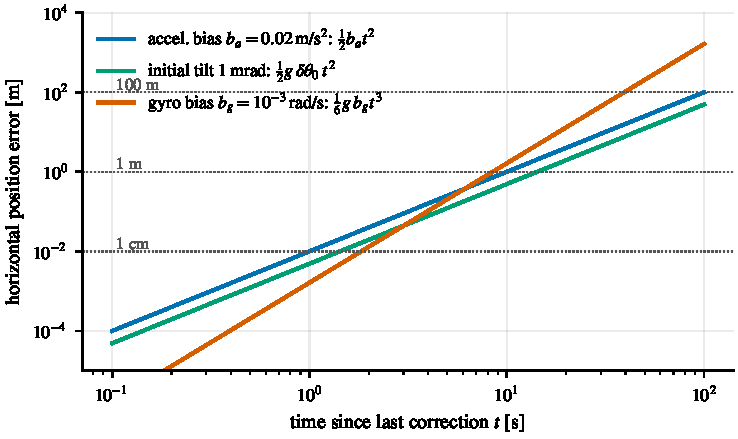
\includegraphics[width=0.86\textwidth]{fig_dr_drift.pdf}
  \caption{Deterministic dead-reckoning drift from three error sources of a consumer-grade IMU.
  A gyro bias of $10^{-3}$~rad/s ($\approx 0.06\,^\circ$/s) produces more than a meter of error
  after ten seconds and hundreds of meters after one minute. The cubic law is why attitude
  accuracy dominates inertial navigation.}
  \label{fig:dr-drift}
\end{figure}

With $b_g = 10^{-3}$~rad/s, a modest value for a MEMS gyroscope, the gyro term alone gives
$1.6$~m after 10~s and $353$~m after 60~s. Random sensor noise adds error that grows in a
similar way. \Cref{ch:errordyn} derives that the position \emph{standard deviation} due to
accelerometer white noise grows as $t^{3/2}$, due to gyroscope white noise as $t^{5/2}$, and due to
the gyroscope bias random walk as $t^{7/2}$.

\begin{keyidea}[inertial navigation is an attitude problem]
Because gravity is large (about $9.81~\mathrm{m/s^2}$) compared with typical accelerometer errors,
a tilt of one milliradian costs as much as an accelerometer bias of about
$10~\mathrm{mm/s^2}$. Position accuracy is therefore limited mostly by attitude accuracy. Any aiding
sensor that constrains roll and pitch, as a camera does, pays off enormously.
\end{keyidea}

\subsection{The camera}

A camera measures the \emph{directions} (bearings) of light rays arriving from the scene. A point
$p_f$ in the world appears in the image at the projection of its camera-frame coordinates
$p_c = (X_c, Y_c, Z_c)$:
\begin{equation}
  z = \begin{bmatrix} X_c/Z_c \\ Y_c/Z_c \end{bmatrix}.
\end{equation}
Because images are measurements of fixed scene geometry, they do not drift the way integrated
inertial data does. But a single camera has a fundamental blind spot.

\begin{proposition}[Monocular scale ambiguity]
\label{prop:scale-ambiguity}
Let a camera with poses $(R_i, p_i)$, $i = 1, \dots, M$, observe points $p_{f,j}$. For any $s > 0$, the
scaled configuration with poses $(R_i, s\,p_i)$ and points $s\,p_{f,j}$ produces exactly the same
images.
\end{proposition}
\begin{proof}
In camera $i$, the scaled point has coordinates
$R_i\T(s\,p_{f,j} - s\,p_i) = s\, R_i\T(p_{f,j} - p_i)$. The projection divides the first two
coordinates by the third, so the factor $s$ cancels.
\end{proof}

A camera alone therefore recovers the trajectory and the scene only up to an unknown global scale.
A photograph of a toy car from 10~cm can be identical to a photograph of a real car from 4~m. Cameras
also fail under motion blur, in darkness, against texture-less surfaces such as white walls, and in
scenes dominated by moving objects.

\subsection{Why the combination works}

\begin{table}[t]
\centering\small
\begin{tabularx}{\textwidth}{@{}>{\raggedright\arraybackslash}X >{\raggedright\arraybackslash}X >{\raggedright\arraybackslash}X@{}}
\toprule
 & \textbf{IMU} & \textbf{Monocular camera} \\
\midrule
Rate & 100--1000 Hz & 10--60 Hz \\
Measures & angular rate, specific force & bearings to scene points \\
Scale & metric & unknown (\cref{prop:scale-ambiguity}) \\
Drift & fast ($t^2$ to $t^3$) & slow, relative to the scene \\
Gravity direction & observable (at rest or on average) & not observable \\
Fails when & always drifts; saturates on impacts & blur, darkness, no texture, pure rotation \\
\bottomrule
\end{tabularx}
\caption{The IMU and the camera fail in complementary ways.}
\label{tab:sensor-complement}
\end{table}

\Cref{tab:sensor-complement} summarizes the complementarity. The camera bounds the inertial drift by
constraining the motion between images. The IMU supplies metric scale, the direction of gravity
(and hence absolute roll and pitch), high-rate motion between frames, and robustness during brief
visual outages. Scale becomes observable because the accelerometer measures acceleration in
$\mathrm{m/s^2}$: scaling a trajectory by $s$ scales its acceleration by $s$, which the
accelerometer would notice. The exception is unaccelerated motion. At constant velocity, the
scale is unobservable again, which is one of several \emph{degenerate motions} studied in
\cref{ch:observability}.

Even fused, four directions remain unobservable: the three components of global position, and the
rotation about the gravity vector (global yaw). Neither sensor senses where the origin is or which
way north is. VIO estimates these relative to the starting pose, and they drift.

\section{Why fusion is hard}

The difficulty of VIO comes from several sources acting at once.
\begin{enumerate}
  \item \textbf{Nonlinearity.} Rotations enter the equations through products and trigonometric
        functions, and the camera projection divides by depth.
  \item \textbf{Curved state spaces.} Orientations do not live in a vector space. You cannot add
        two rotations, and every estimator must deal with this (\cref{ch:lie}).
  \item \textbf{Multi-rate, asynchronous data.} The IMU runs at 200~Hz and the camera at 20~Hz,
        and every measurement must be processed in timestamp order.
  \item \textbf{Unknown scene.} The 3D positions of the visual features are unknown and must be
        estimated, or eliminated, along with the motion.
  \item \textbf{Outliers.} Feature tracks fail, latch onto moving objects, or slide along edges.
  \item \textbf{Unobservability.} Some directions of the state cannot be determined. A careless
        estimator can become falsely confident about them, which is the consistency problem of
        \cref{ch:observability}.
  \item \textbf{Real time.} All of this must run at camera rate, deterministically, on embedded
        processors.
\end{enumerate}

\section{A map of the field}

VIO algorithms differ along three main axes.

\paragraph{Loosely vs.\ tightly coupled.} A loosely coupled system runs a vision-only pipeline
that produces up-to-scale poses and fuses those poses with the IMU. A tightly coupled system feeds
the raw visual measurements (feature positions in the image) directly into a single estimator
together with the inertial data. Tight coupling is more accurate and more robust, because the IMU
helps the vision part and correlations are handled correctly. All modern high-accuracy systems,
and this project, are tightly coupled.

\paragraph{Filtering vs.\ optimization.} \emph{Filtering} approaches (EKF-based) process each
measurement once, keep a Gaussian belief over a bounded state, and discard the past. They are fast
and have predictable cost. \emph{Optimization} approaches solve a nonlinear least-squares problem
over a sliding window of recent states, relinearizing as needed, and summarize discarded states as
a prior (marginalization). They are typically more accurate per frame but more expensive and more
complex. The two families are closer than they appear: the MSCKF is equivalent to a single
Gauss--Newton iteration over a sliding window of poses with the landmarks marginalized
(\cref{ch:msckfupdate}).

\paragraph{Feature-based vs.\ direct.} Feature-based systems extract and track sparse keypoints and
use their image coordinates as measurements. Direct systems use pixel intensities themselves
(photometric error).

\begin{table}[t]
\centering\small
\begin{tabularx}{\textwidth}{@{}l l >{\raggedright\arraybackslash}X@{}}
\toprule
\textbf{System} & \textbf{Family} & \textbf{Notes} \\
\midrule
EKF-SLAM / MonoSLAM~\cite{davison2007monoslam} & filter, landmarks in state & cost grows quadratically with landmarks \\
MSCKF~\cite{mourikis2007msckf, li2013msckf2} & filter, poses in state & landmarks eliminated by nullspace projection; this project \\
MSCKF-VIO~\cite{sun2018msckfvio} & filter (stereo MSCKF) & open-source, fast flight; good engineering reference \\
OpenVINS~\cite{geneva2020openvins} & filter (MSCKF + SLAM features) & research platform with excellent documentation \\
ROVIO~\cite{bloesch2015rovio} & filter, direct & photometric patches in an iterated EKF \\
OKVIS~\cite{leutenegger2015okvis} & optimization, keyframes & sliding-window bundle adjustment \\
VINS-Mono~\cite{qin2018vins} & optimization & preintegration, robust initialization, loop closure \\
ORB-SLAM3~\cite{campos2021orbslam3} & optimization + map & full visual-inertial SLAM with relocalization \\
\bottomrule
\end{tabularx}
\caption{Representative visual-inertial estimators.}
\label{tab:vio-systems}
\end{table}

\section{Why the MSCKF}

In EKF-SLAM every tracked landmark adds three variables to the state. Covariance updates cost
$\mathcal{O}(n^2)$ to $\mathcal{O}(n^3)$ in the state size $n$, so a few hundred landmarks quickly
exhaust a real-time budget, and landmark initialization from a single camera is awkward because
depth is unknown at first sight.

The \textbf{Multi-State Constraint Kalman Filter} of Mourikis and Roumeliotis~\cite{mourikis2007msckf}
keeps instead a sliding window of past IMU poses, called \emph{clones}, taken at image times. When a
feature has been tracked across several clones, its observations constrain those poses relative to
one another. The feature's 3D position is triangulated temporarily, then algebraically
eliminated from the linearized equations by projecting onto the left nullspace of its Jacobian
(\cref{ch:msckfupdate}). The landmark never enters the state. The result:
\begin{itemize}
  \item cost linear in the number of features and bounded by the window size;
  \item no need to initialize landmark depth inside the filter;
  \item all the geometric information of each feature track is used exactly once.
\end{itemize}
These properties make the MSCKF the canonical filter-based VIO and an excellent vehicle for
learning, because it requires every ingredient of the field to be understood and nothing more.

\section{The estimator at a glance}

\begin{figure}[t]
\centering
\begin{tikzpicture}[node distance=7mm and 11mm]
  \node[block] (imu) {IMU\\ \footnotesize 200 Hz};
  \node[block, right=of imu] (prop) {Nominal propagation\\ \footnotesize Ch.~\ref{ch:strapdown}};
  \node[block, right=of prop] (cov) {Covariance propagation\\ \footnotesize Ch.~\ref{ch:errordyn}};
  \node[block, below=10mm of imu] (cam) {Camera\\ \footnotesize 20 Hz};
  \node[block, right=of cam] (front) {Front end: detect,\\ track, reject\\ \footnotesize Ch.~\ref{ch:frontend}};
  \node[block, right=of front] (clone) {Clone pose,\\ augment $P$\\ \footnotesize Ch.~\ref{ch:cloning}};
  \node[block, below=10mm of clone] (upd) {MSCKF update:\\ triangulate, project,\\ gate, update\\ \footnotesize Ch.~\ref{ch:msckfupdate}};
  \node[block, left=of upd] (inj) {Inject, reset,\\ marginalize\\ \footnotesize Ch.~\ref{ch:eskf}, \ref{ch:cloning}};
  \node[block, below=8mm of inj, fill=white] (out) {Pose, velocity,\\ biases, covariance};
  \coordinate (L) at ($(cam.west)+(-7mm,0)$);
  \coordinate (T) at ($(imu.north)+(0,6mm)$);
  \draw[->] (imu) -- (prop);
  \draw[->] (prop) -- (cov);
  \draw[->] (cam) -- (front);
  \draw[->] (front) -- node[note, above]{tracks} (clone);
  \draw[->] (cov) -- (clone);
  \draw[->] (clone) -- (upd);
  \draw[->] (upd) -- (inj);
  \draw[->] (inj) -- (out);
  \draw[->, dashed] (inj.west) -| (L) -- (L |- T) -| node[note, above, pos=0.25]{corrected state feeds back into propagation} (prop.north);
\end{tikzpicture}
\caption{Data flow of the monocular MSCKF built in these notes.}
\label{fig:pipeline}
\end{figure}

\Cref{fig:pipeline} shows the whole estimator. Between images, each IMU sample advances the nominal
state with the nonlinear kinematics and grows the error covariance. When an image arrives, the
filter propagates exactly to the image timestamp, appends a clone of the current pose, and updates
the feature tracks. Tracks that have ended, or whose oldest observation is about to leave the window,
are triangulated and converted into constraints between clones. The update corrects the IMU state and
all clones together, the correction is injected into the nominal state, and the oldest clone is
removed when the window is full. \Cref{ch:planar} builds a complete miniature of this pipeline for a robot moving in a plane,
small enough to derive by hand and to run as a short Python script; it is the place to look whenever the general chapters
feel abstract.

\begin{projectlink}[the road map]
The project builds this pipeline from the bottom up: the Lie group toolkit (M2), the data
stream (M3), inertial propagation (M4--M5), a filter tested against synthetic pose measurements
(M6--M7), the visual front end (M8--M9), and finally the MSCKF (M10a--M10b). Each layer is tested
in isolation before the next is added, so that any later failure can be localized.
\end{projectlink}

\section{The EuRoC benchmark}

The European Robotics Challenge (EuRoC) MAV dataset~\cite{burri2016euroc} is the standard VIO
benchmark. A hexacopter carries a stereo pair of global-shutter cameras ($752 \times 480$, 20~Hz)
and an ADIS16448 MEMS IMU (200~Hz), hardware-synchronized and calibrated. Eleven sequences fly
through an industrial machine hall (MH\_01 to MH\_05) and a motion-capture room (V1\_01 to V2\_03),
graded easy, medium and difficult by speed, lighting and texture. Ground truth comes from a laser
tracker or a motion-capture system. \Cref{app:euroc} documents the file formats and calibration
values the project uses.

\begin{takeaways}
\begin{itemize}
  \item VIO estimates pose, velocity and IMU biases from an IMU and a camera, with no map and no
        absolute positioning, and its error grows without bound.
  \item Inertial drift is dominated by attitude error: a gyro bias produces position error growing
        like $t^3$.
  \item A monocular camera observes the scene only up to scale. The accelerometer supplies the
        scale, provided the body accelerates.
  \item Global position and yaw remain unobservable even with both sensors.
  \item The MSCKF keeps a sliding window of past poses rather than landmarks, which bounds its cost
        while using every feature track.
\end{itemize}
\end{takeaways}

\begin{exercises}
  \item A MEMS accelerometer has a bias of $5~\mathrm{mg}$ ($1\,\mathrm{mg} = 9.81\times10^{-3}~\mathrm{m/s^2}$).
        How long can you dead-reckon before the position error exceeds 1~m? What gyro bias produces
        the same error at the same time?
  \item Prove that the gravity leak produced by a constant tilt error $\delta\theta_0$ is
        $g\,\delta\theta_0$ to first order. What is the exact expression, and at what tilt does the
        first-order formula err by 1\%?
  \item Extend \cref{prop:scale-ambiguity}: show that applying a common rigid transformation
        $(R, t)$ to all camera poses and points also leaves the images unchanged. How many
        unobservable degrees of freedom does a monocular camera have? Which of them does an IMU
        remove, and why?
  \item A drone hovers perfectly still for 30~s. Which states can a VIO system estimate during that
        time, and which cannot be distinguished from each other? (Revisit this after
        \cref{ch:observability}.)
  \item Read the abstract and introduction of~\cite{mourikis2007msckf}. In two sentences, state the
        problem with EKF-SLAM that the paper claims to solve, and the key idea of the solution.
\end{exercises}


\part{Mathematical Foundations}
\chapter{Linear Algebra for State Estimation}
\label{ch:linalg}

\begin{objectives}
\begin{itemize}
  \item Master the cross-product matrix $\sx{a}$ and the identities used in every Jacobian derivation.
  \item Understand the four fundamental subspaces, especially the \emph{left nullspace} on which the
        MSCKF rests.
  \item Know when and why to use Cholesky, LDL$^\mathsf{T}$, QR and SVD, and why a filter should never
        form an explicit inverse.
  \item Use block matrices, Schur complements and the Woodbury identity fluently.
  \item Understand the matrix exponential and floating-point arithmetic well enough to write
        numerically robust code.
\end{itemize}
\end{objectives}

Most of the computation in a Kalman filter is linear algebra: products of covariance matrices,
solutions of linear systems, and factorizations. This chapter collects the tools the rest of the
notes rely on and explains the numerical reasoning behind them. Readers fluent in numerical linear
algebra can skim it, but should not skip \cref{sec:skew,sec:subspaces,sec:floating}.

% ------------------------------------------------------------------------------
\section{Vectors, coordinates and the cross product}
\label{sec:skew}

\subsection{Vectors versus their coordinates}

A physical vector, such as a velocity or the direction of gravity, exists independently of any
coordinate system. To compute with it we express it in a \emph{frame}: an origin plus three
orthonormal, right-handed axes. The same physical vector $\vec{v}$ has different coordinate
triples $v_w \in \R^3$ and $v_b \in \R^3$ in the world and body frames, and the two are related by
a rotation matrix, $v_w = R_{wb}\,v_b$ (\cref{ch:rotations}). Confusing a vector with its
coordinates in some frame is the root of most frame bugs. Throughout these notes, a subscript on a
coordinate vector names the frame it is expressed in.

For coordinate vectors $a, b \in \R^3$ we use the standard inner product
$a\T b = \sum_i a_i b_i$, the Euclidean norm $\|a\| = \sqrt{a\T a}$, and the cross product
$a \times b$. The cross product is bilinear, anti-commutative ($a \times b = -b \times a$), and
orthogonal to both arguments. Its norm is $\|a\|\|b\|\sin\angle(a,b)$.

\subsection{The cross-product (skew-symmetric) matrix}

Because $a \times b$ is linear in $b$, it can be written as a matrix-vector product.

\begin{definition}[Skew-symmetric matrix]
For $a = (a_1, a_2, a_3)\T$, the \emph{cross-product matrix} of $a$ is
\begin{equation}
  \sx{a} = \begin{bmatrix} 0 & -a_3 & a_2 \\ a_3 & 0 & -a_1 \\ -a_2 & a_1 & 0 \end{bmatrix},
  \qquad\text{so that}\qquad \sx{a}\, b = a \times b \quad \forall\, b \in \R^3 .
  \label{eq:skew}
\end{equation}
It is skew-symmetric: $\sx{a}\T = -\sx{a}$. Conversely, every $3\times3$ skew-symmetric matrix
$S$ equals $\sx{s}$ for the unique vector $s = (S_{32}, S_{13}, S_{21})\T$. We write
$s = S\veeop$ for this inverse operation, the \emph{vee} map. In Lie theory, $\sx{\cdot}$ is
also written $(\cdot)\hatop$ and called the \emph{hat} map.
\end{definition}

The following identities are used constantly in derivations. Learn to recognize them on sight.

\begin{proposition}[Cross-product identities]
\label{prop:skew-identities}
For $a, b, c \in \R^3$ and $R \in \SO$ (a rotation matrix):
\begin{align}
  \sx{a}\, b &= -\sx{b}\, a, \label{eq:skew-anticomm}\\
  \sx{a}\, a &= 0, \label{eq:skew-self}\\
  \sx{a}^2 &= a a\T - \|a\|^2 I, \label{eq:skew-sq}\\
  \sx{a}^3 &= -\|a\|^2 \sx{a}, \label{eq:skew-cube}\\
  \sx{a}\sx{b} &= b a\T - (a\T b)\, I, \label{eq:skew-prod}\\
  \sx{a \times b} &= \sx{a}\sx{b} - \sx{b}\sx{a} = b a\T - a b\T, \label{eq:skew-commutator}\\
  \sx{R a} &= R \sx{a} R\T, \label{eq:skew-rot}\\
  R\,(a \times b) &= (Ra) \times (Rb). \label{eq:cross-rot}
\end{align}
\end{proposition}

\begin{proof}
\eqref{eq:skew-anticomm} and \eqref{eq:skew-self} restate $a\times b = -b\times a$ and
$a \times a = 0$. For \eqref{eq:skew-prod}, apply both sides to an arbitrary $c$ and use the
``BAC--CAB'' rule $a \times (b \times c) = b\,(a\T c) - c\,(a\T b)$:
$\sx{a}\sx{b}c = a\times(b\times c) = b a\T c - (a\T b) c$. Setting $b = a$ gives
\eqref{eq:skew-sq}, and multiplying \eqref{eq:skew-sq} by $\sx{a}$ and using \eqref{eq:skew-self}
gives \eqref{eq:skew-cube}. Subtracting \eqref{eq:skew-prod} from its version with $a, b$ swapped
gives the second equality of \eqref{eq:skew-commutator}. The first follows from the Jacobi identity
$a \times (b \times c) + b \times (c \times a) + c \times (a \times b) = 0$. For
\eqref{eq:cross-rot}, the cross product is defined by orientation and lengths, both preserved by a
proper rotation. Finally \eqref{eq:skew-rot} follows from \eqref{eq:cross-rot}:
$\sx{Ra}\, c = (Ra)\times c = (Ra)\times(R R\T c) = R\big(a \times R\T c\big) = R\sx{a}R\T c$.
\end{proof}

\begin{keyidea}[moving a vector out of a cross product]
Identity \eqref{eq:skew-anticomm} is how unknowns are isolated in Jacobian derivations. A
perturbation appears as $\sx{\delta\theta}\,v$, and the Jacobian with respect to $\delta\theta$ is
read off after rewriting it as $-\sx{v}\,\delta\theta$.
\end{keyidea}

Identity \eqref{eq:skew-cube} is what makes closed-form rotation formulas possible: every power of
$\sx{a}$ reduces to a multiple of $\sx{a}$ or $\sx{a}^2$, so infinite series in $\sx{a}$ collapse
to two terms (\cref{ch:rotations}).

% ------------------------------------------------------------------------------
\section{The four fundamental subspaces}
\label{sec:subspaces}

Let $A \in \R^{m\times n}$ have rank $r$. Four subspaces are associated with it:
\begin{center}
\begin{tabular}{@{}l l l l@{}}
\toprule
Subspace & Definition & Lives in & Dimension \\
\midrule
column space (range) & $\range(A) = \{Ax\}$ & $\R^m$ & $r$ \\
nullspace & $\nullsp(A) = \{x : Ax = 0\}$ & $\R^n$ & $n - r$ \\
row space & $\range(A\T)$ & $\R^n$ & $r$ \\
left nullspace & $\nullsp(A\T) = \{y : y\T A = 0\}$ & $\R^m$ & $m - r$ \\
\bottomrule
\end{tabular}
\end{center}

\begin{theorem}[Fundamental theorem of linear algebra]
\label{thm:fundamental}
$\nullsp(A) = \range(A\T)^\perp$ and $\nullsp(A\T) = \range(A)^\perp$. Consequently
$\R^n = \range(A\T) \oplus \nullsp(A)$ and $\R^m = \range(A) \oplus \nullsp(A\T)$, with
orthogonal direct sums.
\end{theorem}
\begin{proof}
$y \in \nullsp(A\T) \iff A\T y = 0 \iff x\T A\T y = 0\ \forall x \iff (Ax)\T y = 0\ \forall x
\iff y \perp \range(A)$. The first statement is the same argument applied to $A\T$.
\end{proof}

The \emph{left nullspace} deserves special attention because the MSCKF is built on it. Suppose a
stacked measurement depends on an unwanted variable $f$ through a tall matrix $H_f \in \R^{m\times
3}$ of full column rank:
\begin{equation}
  r = H_x\,\delta x + H_f\,\delta f + n .
\end{equation}
Take any matrix $A \in \R^{m\times(m-3)}$ whose columns form an orthonormal basis of
$\nullsp(H_f\T)$. Then $A\T H_f = 0$, and multiplying through by $A\T$ gives
$A\T r = A\T H_x\,\delta x + A\T n$: the unwanted variable has disappeared. \Cref{ch:msckfupdate}
shows that no information about $\delta x$ is lost in the process.

\begin{definition}[Orthogonal projector]
A matrix $\Pi$ is an orthogonal projector if $\Pi^2 = \Pi$ and $\Pi\T = \Pi$. If the columns of
$Q$ are an orthonormal basis of a subspace $\mathcal{S}$, the projector onto $\mathcal{S}$ is
$\Pi_{\mathcal{S}} = Q Q\T$. If $A$ has full column rank, the projector onto $\range(A)$ is
$A (A\T A)\inv A\T$, and $I - \Pi_{\mathcal{S}}$ projects onto $\mathcal{S}^\perp$.
\end{definition}

For the matrix $A$ spanning the left nullspace of $H_f$, these facts combine into an identity we
will use to prove the MSCKF's optimality:
\begin{equation}
  A A\T = I - H_f (H_f\T H_f)\inv H_f\T .
  \label{eq:nullspace-projector}
\end{equation}

% ------------------------------------------------------------------------------
\section{Symmetric and positive-definite matrices}

Covariance matrices are symmetric and positive semi-definite, and much of the numerical care in a
filter goes into keeping them that way.

\begin{definition}
A symmetric matrix $P = P\T \in \R^{n\times n}$ is \emph{positive semi-definite} (PSD, $P \succeq 0$) if
$x\T P x \ge 0$ for all $x$, and \emph{positive definite} (PD, $P \succ 0$) if $x\T P x > 0$
for all $x \ne 0$. We write $P_1 \succeq P_2$ (the Loewner order) if $P_1 - P_2 \succeq 0$.
\end{definition}

\begin{theorem}[Spectral theorem]
Every real symmetric matrix factors as $P = U \Lambda U\T$ with $U$ orthogonal and
$\Lambda = \diag(\lambda_1,\dots,\lambda_n)$ real. $P \succeq 0$ if and only if all
$\lambda_i \ge 0$, and $P \succ 0$ if and only if all $\lambda_i > 0$.
\end{theorem}

The geometric picture is an ellipsoid. For $P \succ 0$, the set $\{x : x\T P\inv x \le 1\}$ is an
ellipsoid with principal axes along the columns of $U$ and semi-axis lengths $\sqrt{\lambda_i}$.
This is the ``one-sigma'' uncertainty ellipsoid of a Gaussian with covariance $P$
(\cref{ch:prob}).

\begin{proposition}[Properties of PSD matrices]
\label{prop:psd}
Let $P, Q \succeq 0$ and let $A$ be any matrix of compatible size. Then
\begin{enumerate}
  \item $A P A\T \succeq 0$ (congruence preserves semi-definiteness);
  \item $P + Q \succeq 0$, and $P + Q \succ 0$ if either is PD;
  \item $P_{ii} \ge 0$ and $|P_{ij}| \le \sqrt{P_{ii} P_{jj}}$;
  \item every principal submatrix of $P$ is PSD.
\end{enumerate}
\end{proposition}
\begin{proof}
(1) $x\T A P A\T x = (A\T x)\T P (A\T x) \ge 0$. (2) is immediate. (3) and (4) follow from (1) with
$A$ a selection matrix, using the $2\times2$ determinant for the off-diagonal bound.
\end{proof}

Property (1) explains why the covariance updates $\Phi P \Phi\T + Q$ and the Joseph form
(\cref{ch:kf}) preserve semi-definiteness exactly in exact arithmetic: they are sums of congruences
of PSD matrices. The simpler update $(I - KH)P$ is \emph{not} a congruence, which is why it can lose
positive semi-definiteness under rounding.

% ------------------------------------------------------------------------------
\section{Matrix factorizations}

\subsection{Cholesky and LDL$^\mathsf{T}$}

\begin{theorem}[Cholesky factorization]
A symmetric matrix $S$ is positive definite if and only if $S = L L\T$ for a unique lower
triangular $L$ with positive diagonal.
\end{theorem}

The factor is computed column by column:
\begin{equation}
  L_{jj} = \Big( S_{jj} - \sum_{k<j} L_{jk}^2 \Big)^{1/2}, \qquad
  L_{ij} = \frac{1}{L_{jj}}\Big( S_{ij} - \sum_{k<j} L_{ik}L_{jk} \Big), \quad i > j,
\end{equation}
at a cost of about $n^3/3$ flops, half that of an LU factorization. The algorithm is backward
stable without pivoting, and it fails (a negative argument of the square root) exactly when $S$ is
not numerically positive definite. That makes it a useful diagnostic too. The variant
$S = L D L\T$ with unit-diagonal $L$ and diagonal $D$ avoids square roots, and with symmetric
pivoting (Eigen's \code{LDLT}) it also handles semi-definite matrices gracefully.

Cholesky factors \emph{whiten} correlated quantities. If $n \sim \N(0, S)$ and $S = LL\T$, then
$L\inv n \sim \N(0, I)$. This is how Mahalanobis distances are computed stably:
$r\T S\inv r = \|L\inv r\|^2$, with one triangular solve.

\subsection{QR factorization and Householder reflections}

\begin{definition}[Householder reflection]
For a nonzero $v \in \R^m$, the matrix $H_v = I - 2\, \dfrac{v v\T}{v\T v}$ reflects vectors across
the hyperplane orthogonal to $v$. It is symmetric and orthogonal, $H_v = H_v\T = H_v\inv$.
\end{definition}

Given any $x \in \R^m$, choosing $v = x + \operatorname{sign}(x_1)\|x\|\,e_1$ gives
$H_v x = -\operatorname{sign}(x_1)\|x\|\,e_1$: a single reflection zeroes every entry of $x$ below
the first. (The sign choice avoids cancellation when $x$ is already nearly parallel to $e_1$.)
Applying such reflections to the columns of $A \in \R^{m\times n}$, $m \ge n$, one after another
produces
\begin{equation}
  H_n \cdots H_2 H_1\, A = \begin{bmatrix} R_1 \\ 0 \end{bmatrix}
  \quad\Longleftrightarrow\quad
  A = Q \begin{bmatrix} R_1 \\ 0 \end{bmatrix} = \begin{bmatrix} Q_1 & Q_2 \end{bmatrix}
      \begin{bmatrix} R_1 \\ 0 \end{bmatrix} = Q_1 R_1,
  \label{eq:qr}
\end{equation}
with $Q = H_1 H_2\cdots H_n$ orthogonal, $R_1 \in \R^{n\times n}$ upper triangular, $Q_1 \in
\R^{m\times n}$ and $Q_2 \in \R^{m\times(m-n)}$. The cost is about $2mn^2 - \tfrac23 n^3$ flops.

\begin{proposition}[Nullspaces from QR]
\label{prop:qr-nullspace}
If $A$ has full column rank $n$ and $A = Q_1 R_1$ as in \eqref{eq:qr}, then the columns of $Q_1$
are an orthonormal basis of $\range(A)$ and the columns of $Q_2$ are an orthonormal basis of the
left nullspace $\nullsp(A\T)$. In particular $Q_2\T A = 0$.
\end{proposition}
\begin{proof}
$Q\T A = [R_1;\ 0]$, so $Q_2\T A = 0$. The columns of $Q_2$ are orthonormal and there are $m - n$ of
them, which is the dimension of $\nullsp(A\T)$.
\end{proof}

\begin{implnote}[never form $Q$]
$Q$ is $m\times m$ and dense, but it is defined by only $n$ reflection vectors. Libraries store
those vectors compactly in the lower triangle of the factored matrix. To compute $Q\T B$ for some
other matrix $B$, apply the $n$ reflections to $B$ one at a time, at a cost of $\mathcal{O}(mnk)$
for $B \in \R^{m\times k}$. Forming $Q$ explicitly would cost $\mathcal{O}(m^2 n)$ and $m^2$ storage.
In Eigen, \code{HouseholderQR::householderQ()} returns a lazy \code{HouseholderSequence} that can
be applied to $B$ without materializing $Q$. Whether a particular call allocates must be checked
with the allocation guard, not assumed.
\end{implnote}

A \emph{Givens rotation} zeroes a single entry by rotating two rows. It is the tool of choice when
the matrix is already nearly triangular or very sparse. The original MSCKF paper suggests Givens
rotations for its nullspace projection, because the feature Jacobian has a sparse block structure.

\subsection{The singular value decomposition}

\begin{theorem}[SVD]
Every $A \in \R^{m\times n}$ factors as $A = U \Sigma V\T$ with $U, V$ orthogonal and $\Sigma$
diagonal with entries $\sigma_1 \ge \sigma_2 \ge \dots \ge 0$, the \emph{singular values}.
\end{theorem}

The SVD reveals everything about $A$ at once. The rank is the number of nonzero singular values; the
first $r$ columns of $U$ and $V$ span the column and row spaces, and the remaining columns span the
left nullspace and the nullspace. The \emph{condition number} $\kappa(A) = \sigma_1/\sigma_n$
measures how much relative errors in the data can be amplified in the solution of a linear system.
The minimum-norm least-squares solution of $Ax \approx b$ is $x = A^+ b$ with the pseudo-inverse
$A^+ = V \Sigma^+ U\T$. The SVD is the most robust of the factorizations and also the most
expensive. In this project it appears in the linear triangulation of \cref{ch:multiview} and in
diagnostics.

% ------------------------------------------------------------------------------
\section{Solving linear systems and least squares}

\begin{pitfall}[explicit inverses]
Formulas such as $K = P H\T S\inv$ are notation, not algorithms. Computing $S\inv$ and then
multiplying costs about three times as much as solving, is less accurate, and destroys structure.
Factor $S$ once (Cholesky or LDL$^\mathsf{T}$) and solve: $S K\T = H P\T$ gives $K\T$ by two
triangular substitutions per column. Writing \code{S.ldlt().solve(Identity)} is still an explicit
inverse in disguise.
\end{pitfall}

\paragraph{Least squares.} Given an overdetermined system $Ax \approx b$ with $A \in \R^{m\times n}$
of full column rank, the least-squares solution minimizes $\|Ax - b\|^2$. Setting the gradient to zero
gives the \emph{normal equations} $A\T A x = A\T b$. They are cheap but square the condition number,
$\kappa(A\T A) = \kappa(A)^2$, which can lose half the significant digits. The QR approach is more
stable: with $A = Q_1R_1$, $\|Ax - b\|^2 = \|R_1 x - Q_1\T b\|^2 + \|Q_2\T b\|^2$, so
$x = R_1\inv Q_1\T b$ by back substitution, and the residual norm is $\|Q_2\T b\|$.

\paragraph{Weighted least squares.} If the errors have covariance $W$, minimize
$(Ax - b)\T W\inv (Ax - b)$. With $W = LL\T$ this is ordinary least squares on the whitened system
$L\inv A x \approx L\inv b$.

% ------------------------------------------------------------------------------
\section{Block matrices and the Schur complement}

Estimation constantly partitions vectors and matrices into blocks: IMU state versus clones, poses
versus landmarks. Block elimination is the basic tool.

\begin{proposition}[Block factorization and inverse]
\label{prop:block-inverse}
Let $M = \begin{bmatrix} A & B \\ C & D \end{bmatrix}$ with $A$ invertible, and define the
\emph{Schur complement} of $A$ in $M$, $M/A := D - C A\inv B$. Then
\begin{equation}
  M = \begin{bmatrix} I & 0 \\ C A\inv & I \end{bmatrix}
      \begin{bmatrix} A & 0 \\ 0 & M/A \end{bmatrix}
      \begin{bmatrix} I & A\inv B \\ 0 & I \end{bmatrix},
  \qquad \det M = \det A \cdot \det(M/A),
\end{equation}
and if $M/A$ is invertible,
\begin{equation}
  M\inv = \begin{bmatrix}
    A\inv + A\inv B\, (M/A)\inv\, C A\inv & -A\inv B\, (M/A)\inv \\
    -(M/A)\inv C A\inv & (M/A)\inv
  \end{bmatrix}.
\end{equation}
\end{proposition}
\begin{proof}
Multiply out the three factors. The inverse is the product of the inverses of the three factors in
reverse order, and the inverses of the unit-triangular block factors are obtained by negating their
off-diagonal blocks.
\end{proof}

For a symmetric $M$ with $A \succ 0$: $M \succ 0$ if and only if $M/A \succ 0$. The Schur
complement is the algebraic form of \emph{eliminating} a block of variables. \Cref{ch:prob} shows it
is exactly Gaussian marginalization in information form and conditioning in covariance form.

\begin{theorem}[Woodbury matrix identity]
\label{thm:woodbury}
For invertible $A$ and $C$ and conformable $U, V$,
\begin{equation}
  (A + U C V)\inv = A\inv - A\inv U \big( C\inv + V A\inv U \big)\inv V A\inv .
\end{equation}
\end{theorem}
\begin{proof}
Write the block matrix $\begin{bmatrix} A & U \\ V & -C\inv\end{bmatrix}$ and compute the
top-left block of its inverse in two ways with \cref{prop:block-inverse}: eliminating $A$ first gives
the right-hand side, and eliminating $-C\inv$ first gives $(A + UCV)\inv$.
\end{proof}

Woodbury connects the two forms of the Kalman update (\cref{ch:kf}). It says that a low-rank update
of a matrix gives a low-rank update of its inverse, which is why an update with $m$ measurements
needs only an $m\times m$ inverse no matter how large the state is.

% ------------------------------------------------------------------------------
\section{The matrix exponential}
\label{sec:matexp}

\begin{definition}
For $A \in \R^{n\times n}$, $\exp(A) = \sum_{k=0}^\infty \frac{A^k}{k!} = I + A + \tfrac12 A^2 + \tfrac16 A^3 + \cdots$.
The series converges absolutely for every $A$.
\end{definition}

\begin{proposition}[Properties of the matrix exponential]
\label{prop:matexp}
\begin{enumerate}
  \item $x(t) = \exp(tA)\, x_0$ is the unique solution of $\dot x = Ax$, $x(0) = x_0$.
  \item $\frac{\dd}{\dd t}\exp(tA) = A \exp(tA) = \exp(tA)\, A$.
  \item $\exp(A)\inv = \exp(-A)$, and $\det\exp(A) = e^{\tr A}$.
  \item $\exp(T A T\inv) = T \exp(A)\, T\inv$ for invertible $T$.
  \item If $AB = BA$ then $\exp(A + B) = \exp(A)\exp(B)$. \textbf{In general this fails.}
\end{enumerate}
\end{proposition}

The failure of property 5 for non-commuting matrices is the algebraic root of everything subtle
about rotations: two rotations generated by $\sx{a}$ and $\sx{b}$ do not compose into the rotation
generated by $\sx{a + b}$. \Cref{ch:lie} measures the discrepancy precisely.

\begin{example}[Nilpotent generator: the double integrator]
\label{ex:double-integrator}
For $F = \begin{bmatrix} 0 & 1 \\ 0 & 0 \end{bmatrix}$, $F^2 = 0$, so the series terminates:
$\exp(F\Dt) = \begin{bmatrix} 1 & \Dt \\ 0 & 1\end{bmatrix}$. This is the exact transition matrix of
position and velocity under zero acceleration. The inertial error dynamics of \cref{ch:errordyn}
have a similar nilpotent structure, so their exponentials can be written in closed form.
\end{example}

% ------------------------------------------------------------------------------
\section{Derivatives and Jacobians}

\begin{definition}[Jacobian layout]
For $f: \R^n \to \R^m$, the Jacobian $\frac{\partial f}{\partial x} \in \R^{m\times n}$ has
entries $\big[\frac{\partial f}{\partial x}\big]_{ij} = \frac{\partial f_i}{\partial x_j}$
(numerator layout), so that $f(x + \delta) = f(x) + \frac{\partial f}{\partial x}\delta +
o(\|\delta\|)$. Column $j$ is the sensitivity of the output to the $j$-th input direction. This
is exactly what a finite-difference test computes column by column.
\end{definition}

With this layout the chain rule reads
$\frac{\partial (g\circ f)}{\partial x} = \frac{\partial g}{\partial y}\big|_{y = f(x)}\frac{\partial f}{\partial x}$,
a product of matrices in the same order as the composition. A few derivatives recur:
\begin{equation}
  \frac{\partial (Ax)}{\partial x} = A, \qquad
  \frac{\partial (a \times x)}{\partial x} = \sx{a}, \qquad
  \frac{\partial (x \times a)}{\partial x} = -\sx{a}, \qquad
  \frac{\partial (x\T S x)}{\partial x} = x\T (S + S\T).
\end{equation}
\Cref{ch:lie} extends Jacobians to functions whose inputs or outputs are rotations.

% ------------------------------------------------------------------------------
\section{Floating-point arithmetic}
\label{sec:floating}

An IEEE~754 \code{double} stores a sign, an 11-bit exponent, and a 53-bit significand (52 stored
bits plus an implicit leading one). Two constants matter:
\begin{itemize}
  \item the \emph{machine epsilon} $\mach = 2^{-52} \approx 2.22\times10^{-16}$, the gap between $1$
        and the next larger double (\code{std::numeric\_limits<double>::epsilon()});
  \item the \emph{unit roundoff} $u = 2^{-53} \approx 1.11\times10^{-16}$: every basic operation
        satisfies $\mathrm{fl}(a \circ b) = (a\circ b)(1 + \delta)$ with $|\delta| \le u$.
\end{itemize}
Relative accuracy is therefore excellent for a single operation. Trouble comes from
\emph{cancellation}: subtracting two nearly equal numbers that each carry a rounding error leaves
a small result whose relative error can be enormous.

\begin{example}[Catastrophic cancellation in $1 - \cos\theta$]
\label{ex:cancellation}
For $\theta = 10^{-5}$, $\cos\theta = 1 - 5\times10^{-11} + \dots$. The stored value of
$\cos\theta$ has an absolute error up to $u \approx 10^{-16}$, so $1 - \cos\theta \approx
5\times 10^{-11}$ is computed with relative error up to $10^{-16}/(5\times10^{-11}) \approx 2\times
10^{-6}$. Dividing by $\theta^2$ to form $(1-\cos\theta)/\theta^2 \approx 1/2$ keeps that relative
error. At $\theta = 10^{-8}$, $\cos\theta$ rounds to exactly $1$, and the computed value is $0$
instead of $1/2$. The Taylor expansion $\tfrac12 - \tfrac{\theta^2}{24} + \cdots$ has no
cancellation at all. \Cref{fig:taylor} in \cref{ch:lie} shows this effect for all the coefficient
functions of the rotation group.
\end{example}

\begin{pitfall}[time stamps in floating point]
EuRoC timestamps are nanoseconds since the Unix epoch, about $1.4\times10^{18}$, which lies between
$2^{60}$ and $2^{61}$. A \code{double} near that value can only represent multiples of
$2^{60-52} = 256$~ns. Converting absolute timestamps to \code{double} therefore quantizes them to
256~ns, and accumulating time by repeated addition of $\Dt$ drifts further. Keep absolute time in
64-bit integers (\code{std::chrono::nanoseconds}) and convert only differences to \code{double}
(AGENTS.md C5).
\end{pitfall}

\paragraph{Finite-difference step size.} A finite-difference derivative is itself a cancellation.
For the central difference $\frac{f(x+h) - f(x-h)}{2h}$, the truncation error is about
$\frac{h^2}{6}|f'''|$ and the rounding error about $\frac{u |f|}{h}$. Their sum is minimized at
\begin{equation}
  h^\star = \left(\frac{3\,u\,|f|}{|f'''|}\right)^{1/3} \approx 10^{-5}\text{ to }10^{-6}
  \quad\text{(for quantities of order one)},
\end{equation}
with a total error of order $u^{2/3} \approx 10^{-11}$. For the one-sided difference the optimal step
is $\sim\sqrt{u} \approx 10^{-8}$ and the error is only $\sim 10^{-8}$. This is why Jacobian tests
use central differences with $h \approx 10^{-6}$ and tolerances around $10^{-6}$ to $10^{-8}$, scaled
to the magnitude of the quantities involved.

\paragraph{Conditioning versus stability.} A problem is \emph{ill-conditioned} if small changes in
its data produce large changes in its exact answer. An algorithm is \emph{unstable} if it produces
much larger errors than the conditioning of the problem justifies. Computing the rotation angle
from a rotation matrix with $\arccos$ near zero angle is an unstable algorithm for a
well-conditioned problem (\cref{ch:lie}). Triangulating a point seen with almost no parallax is an
ill-conditioned problem that no algorithm can rescue (\cref{ch:multiview}).

\begin{takeaways}
\begin{itemize}
  \item $\sx{a}b = a\times b = -\sx{b}a$, $\sx{a}^3 = -\|a\|^2\sx{a}$, and $\sx{Ra} = R\sx{a}R\T$ are
        the workhorses of every rotation derivation.
  \item The left nullspace of a tall matrix is the orthogonal complement of its column space.
        A full QR factorization delivers an orthonormal basis for it.
  \item Covariance updates should be congruences ($APA\T$) plus PSD terms, so that positive
        semi-definiteness is preserved structurally.
  \item Factor and solve; never form an explicit inverse, and never form $Q$ explicitly.
  \item Schur complements eliminate variables; Woodbury converts between large and small inverses.
  \item Cancellation, not single operations, destroys floating-point accuracy. Time stamps belong
        in 64-bit integers.
\end{itemize}
\end{takeaways}

\begin{exercises}
  \item Prove \eqref{eq:skew-commutator} directly from \eqref{eq:skew-prod}, and verify the Jacobi
        identity numerically for random vectors.
  \item Show that the eigenvalues of $\sx{a}$ are $0$ and $\pm i\|a\|$. Which eigenvector belongs to $0$?
  \item Let $H_f \in \R^{2M\times3}$ have full column rank. Compute the dimension of its left
        nullspace for $M = 2, 3, 10$. Prove \eqref{eq:nullspace-projector}.
  \item Show that if $P\succ0$ then $P - K S K\T \succeq 0$ for $S = HPH\T + R$, $K = PH\T S\inv$
        and $R \succ 0$. (Hint: Schur complement of a suitable $2\times2$ block matrix.)
  \item Implement Householder QR in Python for a $10\times3$ matrix and check
        \cref{prop:qr-nullspace} numerically. Then compare the accuracy of solving a least-squares
        problem with $\kappa(A) = 10^8$ by the normal equations and by QR.
  \item Use \cref{thm:woodbury} to show that
        $\big(P\inv + H\T R\inv H\big)\inv = P - PH\T(HPH\T + R)\inv HP$. Which side is cheaper to
        evaluate when $P$ is $75\times75$ and $R$ is $2\times2$? When $R$ is $500\times500$?
  \item What is the spacing of doubles near $2^{30}$ seconds expressed in nanoseconds? Would storing
        time as \code{double} seconds since the epoch be acceptable for a 200~Hz IMU?
  \item For $f(x) = \sin x$ at $x = 1$, plot the error of forward and central differences versus
        $h \in [10^{-16}, 10^{-1}]$ on log axes and locate the optimal step sizes. Compare with the
        formulas above.
\end{exercises}

\chapter{Numerical Linear Algebra}
\label{ch:numlinalg}

\begin{objectives}
\begin{itemize}
  \item Count the cost of matrix operations and understand why a filter must never form an explicit inverse.
  \item Derive the LU, Cholesky, QR and singular value decompositions, and know which one to use when.
  \item Solve least-squares problems stably, and compute nullspaces, projectors and pseudo-inverses.
  \item Use block matrices, Schur complements and the Woodbury identity fluently.
  \item Understand the matrix exponential, and why the exponential of a skew-symmetric matrix is a rotation.
  \item Understand floating-point arithmetic: rounding, cancellation, conditioning and stability.
\end{itemize}
\end{objectives}

\Cref{ch:linalg} described what matrices \emph{are}. This chapter is about computing with them reliably. A Kalman filter
spends nearly all of its time in a few operations: multiplying matrices, solving linear systems with a covariance matrix,
and factorizing Jacobians. Done naively, these operations are slow, lose accuracy, or silently destroy the symmetry and
positive definiteness of covariances. Done well, they are fast and accurate to nearly machine precision.

% ==============================================================================
\section{The cost of matrix operations}

Numerical analysts count \term{flops} (floating-point operations: one addition or multiplication each). Some basic costs
for $n\times n$ matrices:
\begin{center}\small
\begin{tabular}{@{}l l@{}}
\toprule
Operation & Approximate flops \\
\midrule
dot product of two $n$-vectors & $2n$ \\
matrix-vector product & $2n^2$ \\
matrix-matrix product & $2n^3$ \\
solving a triangular system & $n^2$ \\
LU factorization & $\tfrac23n^3$ \\
Cholesky factorization & $\tfrac13n^3$ \\
explicit inverse & $2n^3$ \\
\bottomrule
\end{tabular}
\end{center}
For the MSCKF with $n = 75$, a matrix product costs about $8\times10^5$ flops, a fraction of a millisecond. Costs grow with the cube of
the dimension, which is why filters keep their state small, exploit block structure, and update only the blocks that change.
We write $\mathcal{O}(n^3)$ (``order $n^3$'') to mean ``at most a constant times $n^3$ for large $n$''.

% ==============================================================================
\section{Triangular systems and the LU factorization}

\subsection{Forward and back substitution}

A triangular system is solved by direct substitution. For an upper-triangular $U$ with non-zero diagonal, the last equation
$U_{nn}x_n = b_n$ gives $x_n$, the previous one then gives $x_{n-1}$, and so on:
\begin{equation}
  x_i = \frac{1}{U_{ii}}\Big(b_i - \sum_{j>i}U_{ij}x_j\Big), \qquad i = n, n-1, \dots, 1 .
\end{equation}
This is \term{back substitution}; \emph{forward substitution} solves lower-triangular systems from the top. Each costs about $n^2$
flops. Every method in this chapter reduces a hard problem to one or two triangular solves.

\subsection{LU factorization}

Gaussian elimination (\cref{sec:linsys}) subtracts multiples $\ell_{ik}$ of row $k$ from the rows below it, column by column, until
the matrix is upper triangular. Recording the multipliers in a unit lower-triangular matrix $L$ gives the \term{LU factorization}
\begin{equation}
  A = LU .
\end{equation}
Then $Ax = b$ is solved by forward substitution $Ly = b$ and back substitution $Ux = y$. The factorization costs $\tfrac23n^3$ flops
once; every additional right-hand side costs only $2n^2$.

\paragraph{Pivoting.} Elimination divides by the pivots. A tiny pivot creates huge multipliers that amplify rounding errors.
The classic example is $\begin{bmatrix}10^{-20} & 1\\ 1 & 1\end{bmatrix}$: eliminating with the pivot $10^{-20}$ gives a multiplier
of $10^{20}$, and in double precision the computed solution of $Ax = (1, 2)$ is completely wrong, although the matrix is
perfectly well conditioned. Swapping the two rows first fixes it. \emph{Partial pivoting} always swaps the row with the largest
available pivot into place, giving $PA = LU$ with a permutation matrix $P$. Symmetric positive-definite matrices, which is
what filters mostly factor, need no pivoting at all, as the next section shows.

% ==============================================================================
\section{The Cholesky factorization}

\begin{theorem}[Cholesky factorization]
\label{thm:cholesky}
\index{Cholesky factorization}
A symmetric matrix $S$ is positive definite if and only if $S = LL\T$ for a lower-triangular $L$ with positive diagonal.
This $L$ is unique.
\end{theorem}
\begin{proof}
If $S = LL\T$ with $L$ invertible, then $x\T Sx = \|L\T x\|^2 > 0$ for $x \ne 0$. Conversely, partition
\begin{equation*}
  S = \begin{bmatrix} s_{11} & s\T \\ s & S_{22} \end{bmatrix}
    = \begin{bmatrix} \ell_{11} & 0 \\ \ell & L_{22} \end{bmatrix}\begin{bmatrix} \ell_{11} & \ell\T \\ 0 & L_{22}\T \end{bmatrix}
    = \begin{bmatrix} \ell_{11}^2 & \ell_{11}\ell\T \\ \ell_{11}\ell & \ell\ell\T + L_{22}L_{22}\T \end{bmatrix}.
\end{equation*}
Matching blocks: $\ell_{11} = \sqrt{s_{11}}$ (positive because $s_{11} = e_1\T Se_1 > 0$), $\ell = s/\ell_{11}$, and
$L_{22}L_{22}\T = S_{22} - ss\T/s_{11}$. The last matrix (a Schur complement, \cref{sec:schur}) is again positive definite, so the
construction continues recursively on a matrix one size smaller. Each step is forced, which proves uniqueness.
\end{proof}

Unrolling the recursion column by column gives the algorithm
\begin{equation}
  L_{jj} = \Big( S_{jj} - \sum_{k<j} L_{jk}^2 \Big)^{1/2}, \qquad
  L_{ij} = \frac{1}{L_{jj}}\Big( S_{ij} - \sum_{k<j} L_{ik}L_{jk} \Big), \quad i > j,
\end{equation}
at a cost of $\tfrac13n^3$ flops, half that of LU. The algorithm is backward stable without pivoting, and it fails (the argument
of a square root is not positive) exactly when $S$ is not numerically positive definite, which makes it a useful diagnostic
too. The variant $S = LDL\T$, with unit-diagonal $L$ and diagonal $D$, avoids square roots; with symmetric pivoting (Eigen's
\code{LDLT}) it also handles semi-definite and slightly indefinite matrices gracefully.

\paragraph{Uses of the Cholesky factor.}
\begin{itemize}
  \item \emph{Solving} $Sx = b$: forward-substitute $Ly = b$, back-substitute $L\T x = y$.
  \item \emph{Whitening}: if a random vector $n$ has covariance $S = LL\T$, then $L\inv n$ has covariance $I$ (\cref{ch:prob}).
        Mahalanobis distances are computed as $r\T S\inv r = \|L\inv r\|^2$ with a single triangular solve.
  \item \emph{Sampling}: if $s$ has covariance $I$, then $Ls$ has covariance $S$.
  \item \emph{Determinants}: $\det S = \prod_iL_{ii}^2$, and $\log\det S = 2\sum_i\log L_{ii}$ without overflow.
\end{itemize}

% ==============================================================================
\section{Orthogonal factorizations: QR}

Orthogonal transformations do not amplify errors (they preserve lengths), so factorizations built from them are the most
stable available.

\subsection{QR from Gram--Schmidt}

Applying Gram--Schmidt to the columns $a_1, \dots, a_n$ of a full-column-rank $A \in \R^{m\times n}$ produces orthonormal $q_1, \dots, q_n$
with $a_k = \sum_{j\le k}r_{jk}q_j$, where $r_{jk} = q_j\T a_k$ and $r_{kk} = \|\tilde q_k\|$. In matrix form
\begin{equation}
  A = Q_1R_1, \qquad Q_1 = [q_1 \cdots q_n] \in \R^{m\times n},\quad Q_1\T Q_1 = I,\quad R_1 \text{ upper triangular}.
\end{equation}
This is the \term{QR factorization}. Classical Gram--Schmidt, implemented literally, loses orthogonality in floating point when the
columns are nearly dependent; the computed $q$'s drift away from being orthogonal. Householder reflections avoid this problem.

\subsection{Householder reflections}

\begin{definition}[Householder reflection]
\index{Householder reflection}
For a non-zero $v \in \R^m$, the matrix $H_v = I - 2\, \dfrac{v v\T}{v\T v}$ reflects vectors across the hyperplane orthogonal to $v$:
it reverses the component along $v$ and leaves the orthogonal components unchanged. It is symmetric and orthogonal, and is its own
inverse: $H_v = H_v\T = H_v\inv$.
\end{definition}

\begin{proposition}[Zeroing a vector below its first entry]
For $x \in \R^m$ not a multiple of $e_1$, let $\alpha = -\operatorname{sign}(x_1)\|x\|$ and $v = x - \alpha e_1$. Then $H_vx = \alpha e_1$.
\end{proposition}
\begin{proof}
Because $\|x\| = \|\alpha e_1\|$, the vectors $x$ and $\alpha e_1$ have the same length, so the reflection across the
perpendicular bisector of the segment joining them swaps them. That bisecting hyperplane is orthogonal to $v = x - \alpha e_1$.
Algebraically: $v\T v = 2\|x\|^2 - 2\alpha x_1$ and $v\T x = \|x\|^2 - \alpha x_1 = \tfrac12v\T v$, so
$H_vx = x - 2v\,\frac{v\T x}{v\T v} = x - v = \alpha e_1$.
\end{proof}

The sign choice makes $v_1 = x_1 + \operatorname{sign}(x_1)\|x\|$ a sum of two numbers of the same sign, avoiding the cancellation
that the other choice would suffer when $x$ is nearly parallel to $e_1$.

\paragraph{Householder QR.} Apply a reflection $H_1$ that zeroes the first column of $A$ below the diagonal; then a reflection $H_2$,
acting on rows $2, \dots, m$, that zeroes the second column below the diagonal; and so on for all $n$ columns:
\begin{equation}
  H_n \cdots H_2 H_1\, A = \begin{bmatrix} R_1 \\ 0 \end{bmatrix}
  \quad\Longleftrightarrow\quad
  A = Q \begin{bmatrix} R_1 \\ 0 \end{bmatrix} = \begin{bmatrix} Q_1 & Q_2 \end{bmatrix}
      \begin{bmatrix} R_1 \\ 0 \end{bmatrix} = Q_1 R_1,
  \label{eq:qr}
\end{equation}
with $Q = H_1 H_2\cdots H_n$ orthogonal ($m\times m$), $R_1 \in \R^{n\times n}$ upper triangular, $Q_1 \in \R^{m\times n}$ and $Q_2 \in \R^{m\times(m-n)}$. The
cost is about $2mn^2 - \tfrac23 n^3$ flops. The form $A = Q[R_1; 0]$ is the \emph{full} QR factorization, and $A = Q_1R_1$ the
\emph{thin} one.

\paragraph{Applying $Q\T$ without forming $Q$.} Each $H_k$ is determined by its vector $v_k$, so $Q\T b = H_n\cdots H_1b$ is computed by
applying the reflections one at a time:
\begin{equation}
  b \;\gets\; b - v_k\,\frac{2\,v_k\T b}{v_k\T v_k}, \qquad k = 1, \dots, n,
\end{equation}
at a cost of $\mathcal{O}(m)$ per reflection. Forming $Q$ explicitly would cost $\mathcal{O}(m^2n)$ flops and $m^2$ storage.

\begin{proposition}[Nullspaces from QR]
\label{prop:qr-nullspace}
If $A$ has full column rank $n$ and $A = Q_1 R_1$ as in \eqref{eq:qr}, then the columns of $Q_1$ are an orthonormal basis of
$\range(A)$ and the columns of $Q_2$ are an orthonormal basis of the left nullspace $\nullsp(A\T)$. In particular $Q_2\T A = 0$.
\end{proposition}
\begin{proof}
$Q\T A = [R_1;\ 0]$, so $Q_2\T A = 0$, i.e.\ the columns of $Q_2$ lie in $\nullsp(A\T)$. They are orthonormal and there are $m - n$ of them,
which is the dimension of $\nullsp(A\T)$ by rank--nullity. Since $R_1$ is invertible, $\range(A) = \range(Q_1)$.
\end{proof}

\begin{implnote}[never form $Q$]
Libraries store the Householder vectors compactly in the lower triangle of the factored matrix. In Eigen,
\code{HouseholderQR::householderQ()} returns a lazy \code{HouseholderSequence} that can be applied to another matrix without
materializing $Q$. This is exactly what the MSCKF needs: it applies the reflections that triangularize a feature Jacobian to the
rest of the measurement equations (\cref{ch:msckfupdate}). Whether a particular call allocates must be checked with the allocation
guard, not assumed.
\end{implnote}

\subsection{Givens rotations}

A \term{Givens rotation} zeroes one entry at a time by rotating a pair of rows. To zero $b$ in the pair $(a, b)$, set
$r = \sqrt{a^2 + b^2}$, $c = a/r$ and $s = b/r$:
\begin{equation}
  \begin{bmatrix} c & s \\ -s & c \end{bmatrix}\begin{bmatrix} a \\ b \end{bmatrix} = \begin{bmatrix} r \\ 0 \end{bmatrix}.
\end{equation}
Embedded in an identity matrix, it acts on two rows of a larger matrix and leaves the others untouched. Givens rotations are
preferred when only a few entries need to be zeroed, when the matrix is sparse, or when rows arrive one at a time. The original
MSCKF paper suggests them for its nullspace projection, because the feature Jacobian has a sparse block structure.

% ==============================================================================
\section{Least squares}
\label{sec:least-squares}

\subsection{The problem and the normal equations}

An overdetermined system $Ax \approx b$, with $A \in \R^{m\times n}$, $m > n$, generally has no exact solution. The \term{least-squares}
solution minimizes the squared residual
\begin{equation}
  f(x) = \|Ax - b\|^2 = x\T A\T Ax - 2x\T A\T b + b\T b .
\end{equation}
Setting the gradient $2A\T Ax - 2A\T b$ to zero gives the \term{normal equations}
\begin{equation}
  A\T A\,x = A\T b .
  \label{eq:normal-equations}
\end{equation}
If $A$ has full column rank, $A\T A$ is positive definite (since $x\T A\T Ax = \|Ax\|^2 > 0$ for $x\ne0$), so the solution is unique and is
a minimum.

\paragraph{Geometric meaning.} The normal equations say $A\T(b - Ax) = 0$: the residual is orthogonal to every column of $A$. The fitted
vector $Ax$ is the orthogonal projection of $b$ onto $\range(A)$, the closest point to $b$ that the model can produce.

\begin{definition}[Orthogonal projector]
\index{projector}
A matrix $\Pi$ is an orthogonal projector if $\Pi^2 = \Pi$ and $\Pi\T = \Pi$. If the columns of $Q$ are an orthonormal basis of a subspace
$\mathcal{S}$, the projector onto $\mathcal{S}$ is $\Pi_{\mathcal{S}} = QQ\T$. For $A$ of full column rank the projector onto $\range(A)$ is
$A(A\T A)\inv A\T$, and $I - \Pi$ projects onto the orthogonal complement.
\end{definition}

Combining the two descriptions of the projector onto $\range(A)$, and recalling that the columns of $Q_2$ in \eqref{eq:qr} span its
complement $\nullsp(A\T)$, gives an identity we will use to prove the optimality of the MSCKF: for any $A_\perp$ whose columns are an
orthonormal basis of the left nullspace of a full-column-rank $H_f$,
\begin{equation}
  A_\perp A_\perp\T = I - H_f (H_f\T H_f)\inv H_f\T .
  \label{eq:nullspace-projector}
\end{equation}

\subsection{Three ways to solve}

\paragraph{Cholesky on the normal equations.} Form $A\T A$ ($mn^2$ flops) and factor it. This is the fastest method, but forming
$A\T A$ squares the condition number of the problem (\cref{sec:conditioning}): $\kappa(A\T A) = \kappa(A)^2$. When $\kappa(A) = 10^8$,
the normal equations lose essentially all sixteen significant digits.

\paragraph{QR.} With $A = Q[R_1; 0]$ and the invariance of lengths under $Q\T$,
\begin{equation}
  \|Ax - b\|^2 = \|Q\T(Ax - b)\|^2 = \|R_1x - Q_1\T b\|^2 + \|Q_2\T b\|^2 .
\end{equation}
The second term does not depend on $x$, and the first vanishes for $x = R_1\inv Q_1\T b$, computed by back substitution. The minimum
residual is $\|Q_2\T b\|$. This method works with the condition number of $A$ itself and is the standard choice.

\paragraph{SVD.} The most robust and most expensive method, required when $A$ may be rank deficient (\cref{sec:svd}).

\subsection{Weighted least squares}

When the equations have different reliabilities, with errors of covariance $W$, the right objective weights each residual by its
uncertainty (\cref{ch:estimation}):
\begin{equation}
  \min_x\ (Ax - b)\T W\inv(Ax - b) .
\end{equation}
With $W = LL\T$ this is ordinary least squares on the \emph{whitened} system $L\inv Ax \approx L\inv b$, and the normal equations become
$A\T W\inv A\,x = A\T W\inv b$.

% ==============================================================================
\section{The singular value decomposition}
\label{sec:svd}

\begin{theorem}[Singular value decomposition]
\label{thm:svd}
\index{singular value decomposition}
Every $A \in \R^{m\times n}$ can be written as $A = U\Sigma V\T$ with $U \in \R^{m\times m}$ and $V \in \R^{n\times n}$ orthogonal and
$\Sigma \in \R^{m\times n}$ diagonal with entries $\sigma_1 \ge \sigma_2 \ge \dots \ge 0$, the \term{singular values}.
\end{theorem}
\begin{proof}[Construction]
$A\T A$ is symmetric and PSD, so by the spectral theorem $A\T A = V\Lambda V\T$ with orthonormal $v_i$ and eigenvalues
$\lambda_1 \ge \dots \ge \lambda_n \ge 0$. Set $\sigma_i = \sqrt{\lambda_i}$. For each $\sigma_i > 0$ define $u_i = Av_i/\sigma_i$. These are
orthonormal: $u_i\T u_j = v_i\T A\T Av_j/(\sigma_i\sigma_j) = \lambda_jv_i\T v_j/(\sigma_i\sigma_j) = \delta_{ij}$. Complete them to an
orthonormal basis $u_1, \dots, u_m$ of $\R^m$. Then $Av_i = \sigma_iu_i$ for all $i$ (for $\sigma_i = 0$, $\|Av_i\|^2 = \lambda_i = 0$),
which in matrix form is $AV = U\Sigma$.
\end{proof}

\begin{figure}[t]
  \centering
  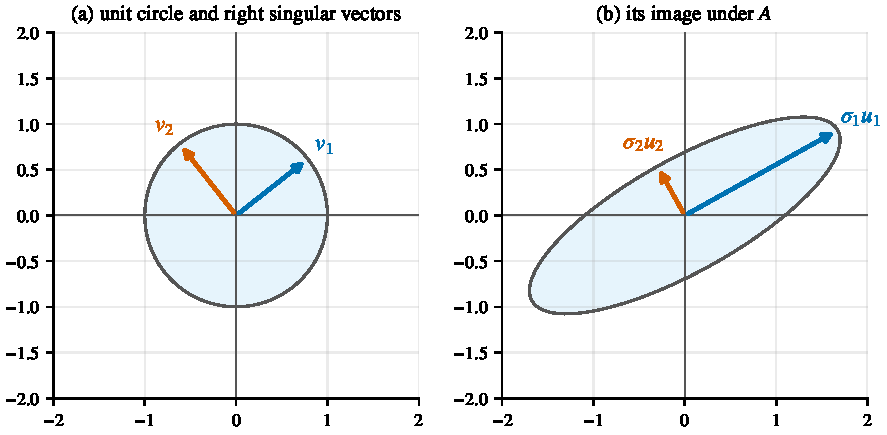
\includegraphics[width=0.9\textwidth]{fig_svd_geometry.pdf}
  \caption{Geometry of the SVD of a $2\times2$ matrix. The right singular vectors $v_1, v_2$ (left) form an orthonormal basis that $A$ maps
  to orthogonal vectors $\sigma_1u_1, \sigma_2u_2$ (right). The unit circle becomes an ellipse with semi-axes $\sigma_1$ and $\sigma_2$: every
  linear map is a rotation, an axis-aligned scaling, and another rotation.}
  \label{fig:svd}
\end{figure}

The SVD says that every linear map, in suitable orthonormal bases of its domain and codomain, is a pure scaling (\cref{fig:svd}). It
reveals everything about $A$ at once:
\begin{itemize}
  \item the rank $r$ is the number of non-zero singular values;
  \item $u_1, \dots, u_r$ span $\range(A)$, $u_{r+1}, \dots, u_m$ span $\nullsp(A\T)$, $v_1, \dots, v_r$ span $\range(A\T)$ and
        $v_{r+1}, \dots, v_n$ span $\nullsp(A)$;
  \item $\|A\|_2 = \sigma_1$ and $\|A\|_F^2 = \sum_i\sigma_i^2$.
\end{itemize}

\paragraph{Pseudo-inverse.} The \term{pseudo-inverse} $A^+ = V\Sigma^+U\T$, where $\Sigma^+$ inverts the non-zero singular values and transposes
the shape, gives the minimum-norm least-squares solution $x = A^+b$ of any system, including rank-deficient ones. For full column
rank, $A^+ = (A\T A)\inv A\T$.

\begin{proposition}[Homogeneous least squares]
\label{prop:homogeneous-ls}
\index{homogeneous least squares}
The unit vector $x$ minimizing $\|Ax\|$ is the right singular vector $v_n$ belonging to the smallest singular value, and the minimum is
$\sigma_n$.
\end{proposition}
\begin{proof}
$\|Ax\|^2 = x\T A\T Ax$, and by the Rayleigh quotient (\cref{prop:rayleigh}) its minimum over unit vectors is the smallest eigenvalue of
$A\T A$, $\sigma_n^2$, attained at the corresponding eigenvector $v_n$.
\end{proof}

Many geometric estimation problems have the form $Ax = 0$ with $x$ known only up to scale: estimating an essential matrix or a homography
from correspondences, or triangulating a point in homogeneous coordinates (\cref{ch:multiview}). With noisy data there is no exact
solution, and \cref{prop:homogeneous-ls} gives the best one.

\begin{theorem}[Best low-rank approximation, Eckart--Young]
\index{Eckart--Young theorem}
Among all matrices of rank at most $k$, the one closest to $A$ in the Frobenius or 2-norm is $A_k = \sum_{i\le k}\sigma_iu_iv_i\T$, obtained by
zeroing all but the $k$ largest singular values.
\end{theorem}

This is how an estimated matrix is projected onto a set defined by its singular values: for example, the nearest valid essential matrix to a
noisy estimate is obtained by replacing its singular values by $(1, 1, 0)$ (\cref{ch:multiview}).

% ==============================================================================
\section{Conditioning and stability}
\label{sec:conditioning}

Two different things can make a computed answer inaccurate: the problem itself may be sensitive to its data, or the algorithm may add more
error than necessary.

\begin{definition}[Condition number]
\index{condition number}
For an invertible (or full-column-rank) $A$, $\kappa(A) = \sigma_{\max}/\sigma_{\min} = \|A\|_2\,\|A^+\|_2$.
\end{definition}

\begin{proposition}[Sensitivity of linear systems]
If $Ax = b$ and $A(x + \delta x) = b + \delta b$, then $\dfrac{\|\delta x\|}{\|x\|} \le \kappa(A)\,\dfrac{\|\delta b\|}{\|b\|}$.
\end{proposition}
\begin{proof}
$\delta x = A\inv\delta b$ gives $\|\delta x\| \le \|A\inv\|\|\delta b\|$, and $b = Ax$ gives $\|b\| \le \|A\|\|x\|$. Multiply the two
inequalities.
\end{proof}

A problem with condition number $\kappa$ can lose about $\log_{10}\kappa$ significant digits whatever the algorithm; it is
\emph{ill-conditioned} when $\kappa$ is large. An algorithm is \emph{backward stable} if its computed answer is the exact answer to a
problem whose data differ from the true data by a few units of rounding error; such an algorithm never loses more than the
conditioning dictates. Householder QR, Cholesky on positive-definite matrices and LU with partial pivoting are backward stable in
practice; classical Gram--Schmidt and the normal equations for ill-conditioned least squares are not. In geometric terms:
triangulating a point seen with almost no parallax is an ill-conditioned problem that no algorithm can rescue
(\cref{ch:multiview}), while recovering the rotation angle from a rotation matrix with $\arccos$ is an unstable algorithm for a
well-conditioned problem (\cref{ch:lie}).

\begin{pitfall}[explicit inverses]
Formulas such as $K = P H\T S\inv$ are notation, not algorithms. Computing $S\inv$ and then multiplying costs about three times as much as
solving, is less accurate, and destroys structure. Factor $S$ once (Cholesky or LDL$^\mathsf{T}$) and solve: $S K\T = H P\T$ gives $K\T$
by two triangular substitutions per column. Writing \code{S.ldlt().solve(Identity)} is still an explicit inverse in disguise.
\end{pitfall}

% ==============================================================================
\section{Block matrices and the Schur complement}
\label{sec:schur}

Estimation constantly partitions vectors and matrices into blocks: IMU state versus clones, poses versus landmarks. Block elimination is
the basic tool.

\begin{proposition}[Block factorization and inverse]
\label{prop:block-inverse}
\index{Schur complement}
Let $M = \begin{bmatrix} A & B \\ C & D \end{bmatrix}$ with $A$ invertible, and define the \term{Schur complement} of $A$ in $M$,
$M/A := D - C A\inv B$. Then
\begin{equation}
  M = \begin{bmatrix} I & 0 \\ C A\inv & I \end{bmatrix}
      \begin{bmatrix} A & 0 \\ 0 & M/A \end{bmatrix}
      \begin{bmatrix} I & A\inv B \\ 0 & I \end{bmatrix},
  \qquad \det M = \det A \cdot \det(M/A),
\end{equation}
and if $M/A$ is invertible,
\begin{equation}
  M\inv = \begin{bmatrix}
    A\inv + A\inv B\, (M/A)\inv\, C A\inv & -A\inv B\, (M/A)\inv \\
    -(M/A)\inv C A\inv & (M/A)\inv
  \end{bmatrix}.
\end{equation}
\end{proposition}
\begin{proof}
Multiply out the three factors. The inverse is the product of the inverses of the three factors in reverse order, and the inverse of a
unit block-triangular factor is obtained by negating its off-diagonal block.
\end{proof}

The Schur complement is what remains of the equations for the second block of unknowns after the first block has been eliminated. To see
this, solve $\begin{bmatrix}A & B\\C & D\end{bmatrix}\begin{bmatrix}x\\y\end{bmatrix} = \begin{bmatrix}f\\g\end{bmatrix}$ by eliminating
$x = A\inv(f - By)$ from the second equation: $(D - CA\inv B)\,y = g - CA\inv f$. For symmetric $M$ with $A \succ 0$, $M \succ 0$ if and only if
$M/A \succ 0$. \Cref{ch:prob} shows that the Schur complement is exactly Gaussian conditioning in covariance form and marginalization in
information form, and \cref{ch:nlls} uses it to eliminate landmarks from bundle adjustment.

\begin{theorem}[Woodbury matrix identity]
\label{thm:woodbury}
\index{Woodbury identity}
For invertible $A$ and $C$ and conformable $U, V$,
\begin{equation}
  (A + U C V)\inv = A\inv - A\inv U \big( C\inv + V A\inv U \big)\inv V A\inv .
\end{equation}
\end{theorem}
\begin{proof}
Write the block matrix $M = \begin{bmatrix} A & U \\ V & -C\inv\end{bmatrix}$ and compute the top-left block of $M\inv$ in two ways with
\cref{prop:block-inverse}. Eliminating $A$ first gives $A\inv + A\inv U(-C\inv - VA\inv U)\inv VA\inv$, the right-hand side. Eliminating the
bottom-right block $-C\inv$ first (the same proposition with the roles of the blocks exchanged) gives the inverse of its Schur complement,
$(A - U(-C\inv)\inv V)\inv = (A + UCV)\inv$.
\end{proof}

Woodbury connects the two forms of the Kalman update (\cref{ch:kf}). It says that a low-rank update of a matrix gives a low-rank update of
its inverse, which is why an update with $m$ measurements needs only an $m\times m$ inverse no matter how large the state is. Its
determinant counterpart is the \emph{matrix determinant lemma} $\det(A + UCV) = \det(C\inv + VA\inv U)\det C\det A$.

% ==============================================================================
\section{The matrix exponential}
\label{sec:matexp}

\begin{definition}[Matrix exponential]
\index{matrix exponential}
For $A \in \R^{n\times n}$, $\exp(A) = \sum_{k=0}^\infty \frac{A^k}{k!} = I + A + \tfrac12 A^2 + \tfrac16 A^3 + \cdots$.
\end{definition}

The series converges for every $A$: the norm of the $k$-th term is at most $\|A\|^k/k!$, and $\sum_k\|A\|^k/k! = e^{\|A\|}$ is finite.

\begin{proposition}[Properties of the matrix exponential]
\label{prop:matexp}
\begin{enumerate}
  \item $\frac{\dd}{\dd t}\exp(tA) = A \exp(tA) = \exp(tA)\, A$.
  \item $x(t) = \exp(tA)\, x_0$ is the unique solution of $\dot x = Ax$, $x(0) = x_0$ (\cref{ch:calculus}).
  \item If $AB = BA$ then $\exp(A + B) = \exp(A)\exp(B)$. \textbf{In general this fails.}
  \item $\exp(A)\inv = \exp(-A)$, and $\exp(A\T) = \exp(A)\T$.
  \item $\exp(T A T\inv) = T \exp(A)\, T\inv$ for invertible $T$.
  \item $\det\exp(A) = e^{\tr A}$.
\end{enumerate}
\end{proposition}
\begin{proof}
(1) Differentiate the series term by term: $\frac{\dd}{\dd t}\frac{t^kA^k}{k!} = A\frac{t^{k-1}A^{k-1}}{(k-1)!}$.
(3) When $A$ and $B$ commute, the binomial theorem holds for $(A + B)^k$, and the Cauchy product of the two series reproduces the series of
$\exp(A + B)$, exactly as for numbers. (4) $A$ and $-A$ commute, so $\exp(A)\exp(-A) = \exp(0) = I$; transposing the series term by term
gives the second statement. (5) $(TAT\inv)^k = TA^kT\inv$. (6) For diagonalizable $A = V\Lambda V\inv$, (5) gives
$\exp(A) = V\exp(\Lambda)V\inv$ with $\exp(\Lambda) = \diag(e^{\lambda_i})$, so $\det\exp(A) = \prod_ie^{\lambda_i} = e^{\sum\lambda_i} = e^{\tr A}$;
the general case follows by continuity, since diagonalizable matrices are dense. Statement (2) is proved in \cref{ch:calculus}.
\end{proof}

The failure of property 3 for non-commuting matrices is the algebraic root of everything subtle about rotations: two rotations generated
by $\sx{a}$ and $\sx{b}$ do not compose into the rotation generated by $\sx{a + b}$. \Cref{ch:lie} measures the discrepancy precisely.

\begin{proposition}[Exponentials of skew-symmetric matrices are rotations]
\label{prop:exp-skew}
If $S\T = -S$ then $\exp(S)$ is a rotation matrix.
\end{proposition}
\begin{proof}
By property 4, $\exp(S)\T\exp(S) = \exp(S\T)\exp(S) = \exp(-S)\exp(S) = I$, so $\exp(S)$ is orthogonal; and
$\det\exp(S) = e^{\tr S} = e^0 = 1$ because a skew-symmetric matrix has a zero diagonal.
\end{proof}

This little proposition is the bridge between the flat world of vectors and the curved world of rotations: every vector $\phi \in \R^3$
defines the rotation $\exp(\sx{\phi})$, and \cref{ch:rotations,ch:lie} show that every rotation arises this way.

\paragraph{Computing the exponential.}
\begin{itemize}
  \item \emph{Nilpotent matrices} ($A^k = 0$ for some $k$): the series is a finite sum.
  \item \emph{Diagonalizable matrices}: $\exp(A) = V\diag(e^{\lambda_i})V\inv$.
  \item \emph{Structured matrices}: when powers of $A$ repeat, as for skew-symmetric $3\times3$ matrices, the series can be summed in closed form
        (Rodrigues' formula, \cref{ch:rotations}).
  \item \emph{General matrices}: \emph{scaling and squaring}. Choose $s$ such that $\|A\|/2^s$ is small, approximate $\exp(A/2^s)$ by a
        truncated series or a rational (Pad\'e) approximation, and square the result $s$ times, using $\exp(A) = \exp(A/2^s)^{2^s}$. This is what
        library routines such as \code{scipy.linalg.expm} do.
\end{itemize}

\begin{example}[Nilpotent generator: the double integrator]
\label{ex:double-integrator}
For $F = \begin{bmatrix} 0 & 1 \\ 0 & 0 \end{bmatrix}$, $F^2 = 0$, so the series terminates:
$\exp(F\Dt) = \begin{bmatrix} 1 & \Dt \\ 0 & 1\end{bmatrix}$. This is the exact transition matrix of position and velocity under zero
acceleration. The inertial error dynamics of \cref{ch:errordyn} have a similar nilpotent structure, so their exponentials can be written in
closed form.
\end{example}

% ==============================================================================
\section{Floating-point arithmetic}
\label{sec:floating}

\subsection{Representation}

\index{floating point}
An IEEE~754 \code{double} represents a number as $\pm1.f\times2^e$, with a sign bit, an 11-bit exponent $e$ and a 52-bit fraction $f$ (53
significant bits counting the implicit leading one). Its range is about $10^{-308}$ to $10^{308}$; results beyond the range \emph{overflow}
to $\pm\infty$, and results below it \emph{underflow} gradually to zero. Undefined operations such as $0/0$ or $\infty - \infty$ produce
\code{NaN} (``not a number''), which propagates through every subsequent operation and compares unequal to everything, including itself.
A single \code{NaN} in a covariance matrix contaminates the whole filter within one update.

\subsection{Rounding}

Two constants describe the precision:
\begin{itemize}
  \item the \term{machine epsilon} $\mach = 2^{-52} \approx 2.22\times10^{-16}$, the gap between $1$ and the next larger double
        (\code{std::numeric\_limits<double>::epsilon()});
  \item the \emph{unit roundoff} $u = 2^{-53} \approx 1.11\times10^{-16}$: every basic operation satisfies
        $\mathrm{fl}(a \circ b) = (a\circ b)(1 + \delta)$ with $|\delta| \le u$.
\end{itemize}
The spacing between consecutive doubles is proportional to their magnitude: near $x$ it is about $\mach|x|$. Relative accuracy is therefore
excellent for a single operation. Errors accumulate in long computations (a sum of $n$ terms can carry a relative error of order $nu$ in the
worst case, though typically $\sqrt n\,u$), but the dramatic losses come from \emph{cancellation}.

\subsection{Cancellation}

Subtracting two nearly equal numbers, each carrying a relative rounding error of size $u$, produces a small result whose \emph{absolute}
error is still of size $u$ times the operands, so its \emph{relative} error can be enormous. The subtraction itself is exact; it merely
exposes the errors already present.

\begin{example}[Catastrophic cancellation in $1 - \cos\theta$]
\label{ex:cancellation}
For $\theta = 10^{-5}$, $\cos\theta = 1 - 5\times10^{-11} + \dots$. The stored value of $\cos\theta$ has an absolute error up to
$u \approx 10^{-16}$, so $1 - \cos\theta \approx 5\times 10^{-11}$ is computed with relative error up to $10^{-16}/(5\times10^{-11}) \approx 2\times
10^{-6}$. Dividing by $\theta^2$ to form $(1-\cos\theta)/\theta^2 \approx 1/2$ keeps that relative error. At $\theta = 10^{-8}$, $\cos\theta$ rounds
to exactly $1$, and the computed value is $0$ instead of $1/2$. The Taylor expansion $\tfrac12 - \tfrac{\theta^2}{24} + \cdots$ has no
cancellation at all. \Cref{fig:taylor} in \cref{ch:lie} shows this effect for all the coefficient functions of the rotation group.
\end{example}

The remedies are always the same: rewrite the expression to avoid the subtraction (for example
$1 - \cos\theta = 2\sin^2(\theta/2)$), use a series expansion in the dangerous regime, or reorganize the algorithm (for example
\code{atan2} instead of \code{acos} for angles, \cref{ch:lie}).

\begin{pitfall}[time stamps in floating point]
EuRoC timestamps are nanoseconds since the Unix epoch, about $1.4\times10^{18}$, which lies between $2^{60}$ and $2^{61}$. A \code{double} near
that value can only represent multiples of $2^{60-52} = 256$~ns. Converting absolute timestamps to \code{double} therefore quantizes them to
256~ns, and accumulating time by repeated addition of $\Dt$ drifts further. Keep absolute time in 64-bit integers
(\code{std::chrono::nanoseconds}) and convert only differences to \code{double} (AGENTS.md C5).
\end{pitfall}

\begin{takeaways}
\begin{itemize}
  \item Costs grow as $n^3$; exploit structure and update only what changes.
  \item Cholesky ($S = LL\T$) is the factorization of choice for covariances: half the cost of LU, stable without pivoting, and a built-in test
        of positive definiteness.
  \item Householder QR is the stable way to solve least squares and to obtain orthonormal bases of a column space and of its complement,
        the left nullspace. Apply $Q\T$ through its reflections; never form $Q$.
  \item The SVD reveals rank, nullspaces and conditioning, and solves homogeneous least squares $\min\|Ax\|$, $\|x\| = 1$.
  \item Schur complements eliminate variables; Woodbury converts between large and small inverses.
  \item $\exp(A + B) \neq \exp(A)\exp(B)$ unless $A$ and $B$ commute; the exponential of a skew-symmetric matrix is a rotation.
  \item Cancellation, not single operations, destroys floating-point accuracy. Time stamps belong in 64-bit integers.
\end{itemize}
\end{takeaways}

\begin{exercises}
  \item Solve $\begin{bmatrix}10^{-20} & 1\\ 1 & 1\end{bmatrix}x = \begin{bmatrix}1\\2\end{bmatrix}$ in double precision by elimination without
        pivoting and with partial pivoting. Explain the difference.
  \item Compute the Cholesky factor of $\begin{bmatrix}4 & 2 & 2\\ 2 & 5 & 3\\ 2 & 3 & 6\end{bmatrix}$ by hand and use it to solve $Sx = (8, 10, 11)$.
  \item Show that if $P\succ0$ then $P - K S K\T \succeq 0$ for $S = HPH\T + R$, $K = PH\T S\inv$ and $R \succ 0$. (Hint: the Schur complement of
        $\begin{bmatrix}S & HP\\ PH\T & P\end{bmatrix}$.)
  \item Implement Householder QR in Python for a $10\times3$ matrix, check \cref{prop:qr-nullspace} numerically, and compare the accuracy of solving
        a least-squares problem with $\kappa(A) = 10^8$ by the normal equations and by QR.
  \item Prove \eqref{eq:nullspace-projector} using a full QR factorization of $H_f$.
  \item Use \cref{thm:woodbury} to show that $\big(P\inv + H\T R\inv H\big)\inv = P - PH\T(HPH\T + R)\inv HP$. Which side is cheaper to evaluate when
        $P$ is $75\times75$ and $R$ is $2\times2$? When $R$ is $500\times500$?
  \item Compute $\exp\big(\begin{bmatrix}0 & -\theta\\ \theta & 0\end{bmatrix}\big)$ by summing the series, and recognize the result.
  \item Show that for $A = \begin{bmatrix}0 & 1\\0 & 0\end{bmatrix}$ and $B = \begin{bmatrix}0 & 0\\1 & 0\end{bmatrix}$,
        $\exp(A + B) \ne \exp(A)\exp(B)$.
  \item What is the spacing of doubles near $2^{30}$ seconds expressed in nanoseconds? Would storing time as \code{double} seconds since the epoch
        be acceptable for a 200~Hz IMU?
  \item Rewrite $\sqrt{x^2 + 1} - x$ for large $x$ and $(1 - \cos x)/x^2$ for small $x$ so that they are computed accurately.
\end{exercises}

\chapter{Calculus, Differential Equations and Numerical Integration}
\label{ch:calculus}
\chaptermark{Calculus and ODEs} % short running header

\begin{objectives}
\begin{itemize}
  \item Use partial derivatives, gradients, Jacobians and Hessians, and the chain rule in matrix form.
  \item Use Taylor's theorem with explicit error terms; this is what ``linearization'' and ``first order'' mean.
  \item Differentiate common matrix expressions: inverses, quadratic forms, determinants.
  \item Solve linear ordinary differential equations, including time-varying ones, with the state transition matrix.
  \item Integrate differential equations numerically, predict the order of the error, and verify it.
  \item Compute derivatives numerically with a step size chosen from first principles.
\end{itemize}
\end{objectives}

A navigation filter is a differential equation (the vehicle's motion) integrated numerically from noisy derivatives (the IMU
readings), corrected with linearized measurement models. This chapter collects the calculus behind those three activities:
derivatives and linearization, differential equations and their solutions, and the numerical methods that approximate both.

% ==============================================================================
\section{Derivatives of functions of several variables}

\subsection{Partial derivatives, gradients and Jacobians}

For a scalar function $f(x_1, \dots, x_n)$, the \emph{partial derivative} $\partial f/\partial x_j$ is the ordinary derivative with respect to
$x_j$ with the other variables held fixed. The \term{gradient} collects them:
$\nabla f = (\partial f/\partial x_1, \dots, \partial f/\partial x_n)\T$. For a vector function $f: \R^n \to \R^m$ the partial derivatives form the
\term{Jacobian} matrix.

\begin{definition}[Jacobian, numerator layout]
For $f: \R^n \to \R^m$, the Jacobian $\frac{\partial f}{\partial x} \in \R^{m\times n}$ has entries
$\big[\frac{\partial f}{\partial x}\big]_{ij} = \frac{\partial f_i}{\partial x_j}$. Row $i$ is the gradient of the $i$-th output (transposed); column $j$ is
the sensitivity of all outputs to the $j$-th input.
\end{definition}

The Jacobian is the matrix of the best linear approximation of $f$ near $x$:
\begin{equation}
  f(x + \delta) = f(x) + \frac{\partial f}{\partial x}\,\delta + o(\|\delta\|),
  \label{eq:linearization}
\end{equation}
where $o(\|\delta\|)$ denotes a remainder that goes to zero faster than $\|\delta\|$. Column $j$ is exactly what a finite-difference
test computes by perturbing the $j$-th input (\cref{sec:numdiff}).

\begin{proposition}[Chain rule]
\label{prop:chain-rule}
\index{chain rule}
If $y = f(x)$ and $z = g(y)$, then $\dfrac{\partial z}{\partial x} = \dfrac{\partial g}{\partial y}\Big|_{y = f(x)}\,\dfrac{\partial f}{\partial x}$.
\end{proposition}
\begin{proof}
Substitute the linear approximation of $f$ into that of $g$:
$g(f(x + \delta)) = g\big(f(x) + J_f\delta + o(\|\delta\|)\big) = g(f(x)) + J_gJ_f\delta + o(\|\delta\|)$.
\end{proof}

With the numerator layout the factors appear in the same order as the composition $g\circ f$, which makes long chains easy to write: the
Jacobian of a camera measurement with respect to a pose is ``(projection) times (frame change) times (pose perturbation)''
(\cref{ch:msckfupdate}).

The \term{Hessian} of a scalar function is the matrix of second derivatives, $[\nabla^2f]_{ij} = \partial^2f/\partial x_i\partial x_j$. For smooth $f$ it is
symmetric. It describes curvature: the second-order behavior of $f$ near a point.

\subsection{Taylor's theorem}

\begin{theorem}[Taylor's theorem in one variable]
\label{thm:taylor}
\index{Taylor's theorem}
If $f$ has $n + 1$ continuous derivatives, then
\begin{equation}
  f(x + h) = \sum_{k=0}^n\frac{f^{(k)}(x)}{k!}h^k + \frac{f^{(n+1)}(\xi)}{(n+1)!}h^{n+1}
\end{equation}
for some $\xi$ between $x$ and $x + h$ (Lagrange form of the remainder).
\end{theorem}

The theorem says more than ``$f$ is close to its Taylor polynomial'': it bounds the error. If $|f^{(n+1)}| \le M$ on the interval, the
error of the degree-$n$ polynomial is at most $Mh^{n+1}/(n+1)!$. This is how we will judge every approximation in these notes.

\begin{figure}[t]
  \centering
  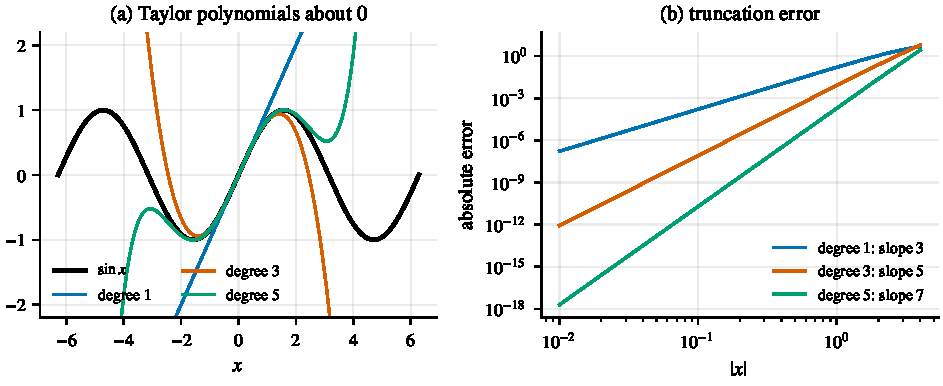
\includegraphics[width=0.95\textwidth]{fig_taylor_sin.pdf}
  \caption{Taylor polynomials of $\sin x$ about $0$ (left) and the absolute error of each (right, log-log scale). Near the expansion point the
  error of the degree-$n$ polynomial falls like $|x|^{n+1}$ or faster. Because the even-order terms of $\sin x$ vanish, the polynomials of degree 1, 3
  and 5 coincide with those of degree 2, 4 and 6, and their errors fall like $|x|^3$, $|x|^5$ and $|x|^7$ (slopes 3, 5 and 7). Far from the
  expansion point, every truncated series fails.}
  \label{fig:taylor-sin}
\end{figure}

\paragraph{Big-O and little-o.} We write $g(h) = O(h^p)$ if $|g(h)| \le Ch^p$ for some constant $C$ as $h\to0$, and $g(h) = o(h^p)$ if
$g(h)/h^p \to 0$. An approximation is \emph{first-order accurate} if its error is $O(h^2)$: the error of a linearization shrinks
quadratically with the size of the perturbation. ``Keeping terms to first order'' in a derivation means writing the result as
linear terms plus an $O(\|\delta\|^2)$ remainder, and then dropping the remainder.

For functions of several variables, Taylor's theorem to second order reads
\begin{equation}
  f(x + \delta) = f(x) + \nabla f(x)\T\delta + \tfrac12\delta\T\nabla^2f(x)\,\delta + O(\|\delta\|^3),
\end{equation}
and for vector functions each component expands this way. The size of the second-order term relative to the first measures how good a
linearization is: when uncertainties are small compared with the scale over which the Jacobian changes, linearization is accurate.
This is the quantitative content of the statement that an extended Kalman filter works well when errors are small (\cref{ch:nonlinear}).

\subsection{Matrix calculus}

A few derivatives recur throughout estimation. We write them as differentials ($\dd f$ = the linear change of $f$ for a small change of the
argument):
\begin{align}
  \dd(Ax) &= A\,\dd x, & \frac{\partial (Ax)}{\partial x} &= A, \\
  \dd(x\T Ax) &= x\T(A + A\T)\,\dd x, & \nabla_x(x\T Ax) &= (A + A\T)x \ \ (= 2Ax \text{ if } A \text{ symmetric}), \\
  \dd(a\times x) &= \sx{a}\,\dd x, & \dd(x \times a) &= -\sx{a}\,\dd x, \\
  \dd(A\inv) &= -A\inv(\dd A)A\inv, & \dd\log\det A &= \tr(A\inv\dd A) .
\end{align}
\begin{proof}[Derivations]
The first and third lines are linear maps, their own derivatives. For the quadratic form,
$(x + \dd x)\T A(x + \dd x) - x\T Ax = \dd x\T Ax + x\T A\,\dd x + O(\|\dd x\|^2) = x\T(A\T + A)\dd x + O(\|\dd x\|^2)$. For the inverse,
differentiate $AA\inv = I$: $(\dd A)A\inv + A\,\dd(A\inv) = 0$. For the log-determinant of a positive-definite $A = U\Lambda U\T$, a small
change $\dd A$ changes each eigenvalue by $u_i\T(\dd A)u_i$ to first order, so
$\dd\sum_i\log\lambda_i = \sum_iu_i\T(\dd A)u_i/\lambda_i = \tr(U\Lambda\inv U\T\dd A) = \tr(A\inv\dd A)$.
\end{proof}

\subsection{Stationary points}

A smooth function has a local minimum at $x^\star$ only if $\nabla f(x^\star) = 0$, and it does have one if, in addition,
$\nabla^2f(x^\star) \succ 0$: by the second-order Taylor expansion, $f(x^\star + \delta) - f(x^\star) = \tfrac12\delta\T\nabla^2f\,\delta + O(\|\delta\|^3) > 0$
for small $\delta \neq 0$. Every least-squares problem in these notes is solved by setting a gradient to zero; \cref{ch:nlls} develops the
iterative methods needed when the resulting equations are nonlinear.

% ==============================================================================
\section{Ordinary differential equations}

\subsection{What a differential equation is}

An \term{ordinary differential equation} (ODE) in state-space form is
\begin{equation}
  \dot x(t) = f\big(x(t), t\big), \qquad x(t_0) = x_0,
\end{equation}
where $x(t) \in \R^n$ is the \emph{state} and $\dot x = \dd x/\dd t$. Any higher-order equation can be put in this form by adding derivatives to
the state: Newton's law $\ddot p = a$ becomes the first-order system $\dot p = v$, $\dot v = a$ with state $(p, v)$. The kinematics of a
navigating vehicle are exactly such a system, with the IMU supplying the right-hand side.

\begin{theorem}[Existence and uniqueness, Picard--Lindel\"of]
\index{Picard--Lindel\"of theorem}
If $f$ is continuous in $t$ and Lipschitz continuous in $x$ (there is an $L$ with $\|f(x, t) - f(y, t)\| \le L\|x - y\|$), the initial value
problem has a unique solution on some interval around $t_0$.
\end{theorem}

Uniqueness is what makes prediction possible: the present state and the inputs determine the future. All the systems in these notes are
smooth enough for the theorem to apply. (A non-example is $\dot x = \sqrt{|x|}$, $x(0) = 0$, solved both by $x \equiv 0$ and by $x = t^2/4$.)

\subsection{Scalar linear equations}

The scalar equation $\dot x = ax + b(t)$ is solved with an \emph{integrating factor}. Multiplying by $e^{-at}$ gives
$\frac{\dd}{\dd t}\big(e^{-at}x\big) = e^{-at}b(t)$; integrating from $t_0$ to $t$,
\begin{equation}
  x(t) = e^{a(t - t_0)}x_0 + \int_{t_0}^t e^{a(t - s)}\,b(s)\,\dd s .
\end{equation}
The solution is the free response of the initial condition plus a weighted sum of the inputs, each propagated from the time it was applied.
Every linear system has this structure.

\subsection{Linear time-invariant systems}

\begin{theorem}[Solution of linear time-invariant systems]
\label{thm:lti-solution}
The solution of $\dot x = Ax + Bu(t)$, $x(t_0) = x_0$, is
\begin{equation}
  x(t) = e^{A(t - t_0)}x_0 + \int_{t_0}^t e^{A(t - s)}Bu(s)\,\dd s .
  \label{eq:lti-solution}
\end{equation}
In particular $\dot x = Ax$ has the unique solution $x(t) = e^{A(t - t_0)}x_0$.
\end{theorem}
\begin{proof}
By \cref{prop:matexp}, $\frac{\dd}{\dd t}\big(e^{-At}x\big) = e^{-At}(\dot x - Ax) = e^{-At}Bu$. Integrating from $t_0$ to $t$ and multiplying by $e^{At}$ gives
\eqref{eq:lti-solution}. The same computation shows that \emph{any} solution satisfies \eqref{eq:lti-solution}, which proves uniqueness.
\end{proof}

The matrix $e^{A\Dt}$ propagates the state over an interval $\Dt$. If $A = V\Lambda V\inv$, the solution is a combination of modes
$e^{\lambda_it}$: decaying for $\operatorname{Re}\lambda_i < 0$, growing for $\operatorname{Re}\lambda_i > 0$, oscillating for imaginary parts. Error
dynamics of inertial navigation have eigenvalues at zero, so their errors grow polynomially rather than exponentially
(\cref{ch:errordyn}).

\subsection{Linear time-varying systems and the state transition matrix}

When the system matrix changes with time, $\dot x = A(t)x$, the exponential no longer applies directly, but its key property survives.

\begin{definition}[State transition matrix]
\index{state transition matrix}
The \term{state transition matrix} $\Phi(t, s)$ of $\dot x = A(t)x$ is the solution of the matrix equation
$\frac{\partial}{\partial t}\Phi(t, s) = A(t)\Phi(t, s)$ with $\Phi(s, s) = I$.
\end{definition}

\begin{proposition}[Properties of the state transition matrix]
\label{prop:stm}
\begin{enumerate}
  \item $x(t) = \Phi(t, s)\,x(s)$ for every solution: $\Phi$ maps states at time $s$ to states at time $t$.
  \item $\Phi(t, s)\,\Phi(s, r) = \Phi(t, r)$ (the semigroup property) and $\Phi(t, s)\inv = \Phi(s, t)$.
  \item For constant $A$, $\Phi(t, s) = e^{A(t - s)}$.
  \item If $A(t)$ commutes with $A(s)$ for all $t, s$, then $\Phi(t, s) = \exp\big(\int_s^tA(\tau)\,\dd\tau\big)$. In general this formula is
        \emph{wrong}.
  \item The solution of $\dot x = A(t)x + B(t)u(t)$ is $x(t) = \Phi(t, t_0)x_0 + \int_{t_0}^t\Phi(t, s)B(s)u(s)\,\dd s$.
\end{enumerate}
\end{proposition}
\begin{proof}
(1) Both $x(t)$ and $\Phi(t, s)x(s)$ solve the ODE with the same value at $t = s$; by uniqueness they agree. (2) Both sides of the first
identity, as functions of $t$, solve the matrix ODE with the value $\Phi(s, r)$ at $t = s$. Setting $r = t$ gives the second. (3) Check that
$e^{A(t-s)}$ satisfies the definition. (4) If the $A(\tau)$ commute, so do $A(t)$ and $M(t) = \int_s^tA$, and then
$\frac{\dd}{\dd t}e^{M(t)} = A(t)e^{M(t)}$ by the commuting case of the series; without commutativity this derivative formula fails.
(5) Differentiate the right-hand side and use (1) and $\frac{\partial}{\partial t}\Phi = A\Phi$.
\end{proof}

Property 4 matters for attitude. The kinematics $\dot R = R\sx{\omega(t)}$ is a linear matrix ODE, and when the angular velocity changes
direction over time the rotation is \emph{not} $\exp\big(\int\sx{\omega}\big)$: rotations about different axes do not commute. Integrating
the angular velocity vector and exponentiating the result produces the ``coning'' error of \cref{ch:strapdown}.

A general series for $\Phi$, the \emph{Peano--Baker series}
\begin{equation*}
  \Phi(t,s) = I + \int_s^tA(\tau_1)\,\dd\tau_1 + \int_s^t\int_s^{\tau_1}A(\tau_1)A(\tau_2)\,\dd\tau_2\,\dd\tau_1 + \cdots,
\end{equation*}
obtained by repeatedly substituting the integral form of the ODE into itself, shows how products of non-commuting matrices enter. In practice $\Phi$ is approximated over short
intervals, where $A$ is nearly constant: $\Phi(t + \Dt, t) \approx \exp(A(t)\Dt) \approx I + A(t)\Dt$, the discretization used by every
filter in these notes.

% ==============================================================================
\section{Numerical integration of ODEs}
\label{sec:numint}

\subsection{Euler's method}

Truncating the Taylor expansion $x(t + h) = x(t) + h\dot x(t) + O(h^2)$ gives \term{Euler's method}:
\begin{equation}
  x_{k+1} = x_k + h\,f(x_k, t_k).
\end{equation}
Each step makes a \emph{local truncation error} of $O(h^2)$. Over a fixed interval $T$ there are $T/h$ steps, so one expects a
\emph{global error} of $O(h)$. The following proposition makes this precise; it also explains why local errors do not simply add up,
but can be amplified by the dynamics.

\begin{proposition}[Global error of Euler's method]
\index{Euler's method}
If $f$ is Lipschitz with constant $L$ and the exact solution has a bounded second derivative $\|\ddot x\| \le M$, the error
$e_k = x_k - x(t_k)$ of Euler's method satisfies $\|e_k\| \le \frac{Mh}{2L}\big(e^{L(t_k - t_0)} - 1\big)$.
\end{proposition}
\begin{proof}
The exact solution satisfies $x(t_{k+1}) = x(t_k) + hf(x(t_k)) + \tau_k$ with $\|\tau_k\| \le Mh^2/2$ by Taylor's theorem. Subtracting from the
numerical step, $e_{k+1} = e_k + h\big(f(x_k) - f(x(t_k))\big) - \tau_k$, so $\|e_{k+1}\| \le (1 + hL)\|e_k\| + Mh^2/2$. With $e_0 = 0$, induction gives
$\|e_k\| \le \frac{Mh^2}{2}\sum_{j<k}(1 + hL)^j = \frac{Mh}{2L}\big((1 + hL)^k - 1\big) \le \frac{Mh}{2L}\big(e^{Lkh} - 1\big)$.
\end{proof}

\begin{definition}[Order of a method]
A method has \emph{order} $p$ if its global error over a fixed interval is $O(h^p)$; equivalently its local error is $O(h^{p+1})$.
\end{definition}

\subsection{Higher-order methods}

\emph{Runge--Kutta} methods evaluate $f$ at several points inside the step and combine the results so that the Taylor expansion of the step
matches the true solution to higher order.
\begin{itemize}
  \item \textbf{Midpoint method} (order 2): $k_1 = f(x_k, t_k)$, $x_{k+1} = x_k + hf(x_k + \tfrac h2k_1, t_k + \tfrac h2)$.
  \item \textbf{Heun's method / trapezoidal rule} (order 2): $k_1 = f(x_k, t_k)$, $k_2 = f(x_k + hk_1, t_k + h)$,
        $x_{k+1} = x_k + \tfrac h2(k_1 + k_2)$.
  \item \textbf{Classical RK4} (order 4): $k_1 = f(x_k, t_k)$, $k_2 = f(x_k + \tfrac h2k_1, t_k + \tfrac h2)$,
        $k_3 = f(x_k + \tfrac h2k_2, t_k + \tfrac h2)$, $k_4 = f(x_k + hk_3, t_k + h)$, $x_{k+1} = x_k + \tfrac h6(k_1 + 2k_2 + 2k_3 + k_4)$.
\end{itemize}
Verifying the order means expanding both the numerical step and the exact solution in Taylor series and comparing coefficients. For Heun's
method on $\dot x = f(x)$: $k_2 = f(x + hf) = f + hf'f + O(h^2)$, so the step is $x + hf + \tfrac{h^2}2f'f + O(h^3)$, which matches
$x(t + h) = x + h\dot x + \tfrac{h^2}2\ddot x + O(h^3)$ because $\ddot x = f'f$.

\begin{figure}[t]
  \centering
  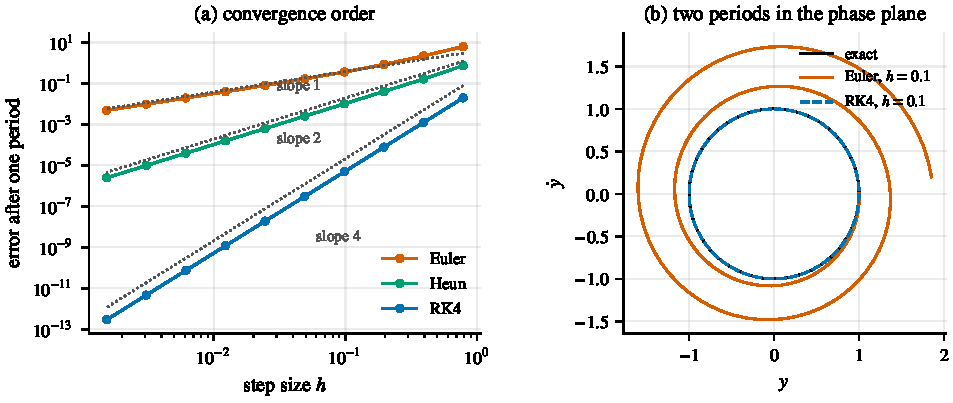
\includegraphics[width=\textwidth]{fig_ode_methods.pdf}
  \caption{Integrating the harmonic oscillator $\ddot y = -y$. (a) Global error after one period versus step size: slopes 1, 2 and 4 confirm the
  orders of Euler, Heun and RK4. (b) With $h = 0.1$, Euler's method spirals outward, gaining energy every step, while RK4 stays on the
  circle to plotting accuracy.}
  \label{fig:ode-methods}
\end{figure}

\paragraph{Verifying the order.} If the error behaves as $Ch^p$, then halving the step divides the error by $2^p$, and the order can be
\emph{measured}: $p \approx \log_2\big(e(h)/e(h/2)\big)$. \Cref{fig:ode-methods}(a) shows this for three methods. A convergence-order test of
this kind is one of the most powerful tests of an integrator: an implementation bug almost always destroys the expected order
(Milestone 4).

\paragraph{Stability.} Euler's method applied to the decaying equation $\dot x = -\lambda x$ gives $x_{k+1} = (1 - h\lambda)x_k$, which blows up
when $h > 2/\lambda$, although the true solution decays. Stiff systems, with very fast decaying modes, need tiny steps or implicit methods.
Applied to an oscillator, Euler's method multiplies the amplitude by $\sqrt{1 + h^2\omega^2} > 1$ per step and spirals outward
(\cref{fig:ode-methods}b). Inertial navigation is not stiff, but this effect is the reason a naive attitude integrator slowly inflates the
norm of its rotation matrix, as we now see.

\subsection{Integrating on a curved space}
\label{sec:lie-euler}

Apply Euler's method to the attitude kinematics $\dot R = R\sx{\omega}$: $R_{k+1} = R_k + hR_k\sx{\omega} = R_k(I + h\sx{\omega})$. The result
is not a rotation matrix:
\begin{equation}
  (I + h\sx{\omega})\T(I + h\sx{\omega}) = I - h^2\sx{\omega}^2 \neq I,
\end{equation}
so every step stretches vectors perpendicular to $\omega$ by a factor of about $1 + \tfrac12h^2\|\omega\|^2$, and the matrix drifts off the set of
rotations. The remedy is to integrate in a way that respects the structure of the space. For constant $\omega$ over the step, the exact
solution is $R_k\exp(h\sx{\omega})$ (\cref{thm:lti-solution}), so the \emph{Lie--Euler} method
\begin{equation}
  R_{k+1} = R_k\exp(h\sx{\omega_k})
\end{equation}
stays exactly on the set of rotations (\cref{prop:exp-skew}) and is first order in general, exact when $\omega$ is constant. Higher-order
generalizations (Runge--Kutta--Munthe-Kaas methods) apply Runge--Kutta to a vector-space parameterization of the increment. Every attitude
update in these notes is multiplicative in this sense (AGENTS.md F1).

% ==============================================================================
\section{Numerical differentiation}
\label{sec:numdiff}

Analytic Jacobians are derived by hand and verified numerically (AGENTS.md E6). Numerical differentiation is easy to write and easy to
get subtly wrong, because it is a subtraction of nearly equal numbers.

\paragraph{Forward differences.} By Taylor's theorem,
\begin{equation}
  \frac{f(x + h) - f(x)}{h} = f'(x) + \frac h2f''(\xi),
\end{equation}
so the \emph{truncation error} is about $\frac h2|f''|$. But $f(x + h)$ and $f(x)$ are each computed with a rounding error of about $u|f|$, and
their difference is divided by $h$, which adds a \emph{rounding error} of about $2u|f|/h$. The total $\frac h2|f''| + \frac{2u|f|}{h}$ is minimized at
$h^\star = 2\sqrt{u|f|/|f''|} \approx 10^{-8}$ for quantities of order one, with a total error of about $10^{-8}$.

\paragraph{Central differences.} Expanding both $f(x \pm h)$,
\begin{equation}
  \frac{f(x + h) - f(x - h)}{2h} = f'(x) + \frac{h^2}{6}f'''(\xi),
\end{equation}
because the even-order terms cancel. The total error $\frac{h^2}6|f'''| + \frac{u|f|}{h}$ is minimized at
\begin{equation}
  h^\star = \left(\frac{3\,u\,|f|}{|f'''|}\right)^{1/3} \approx 10^{-5}\text{ to }10^{-6},
\end{equation}
with a total error of order $u^{2/3} \approx 10^{-11}$.

\begin{figure}[t]
  \centering
  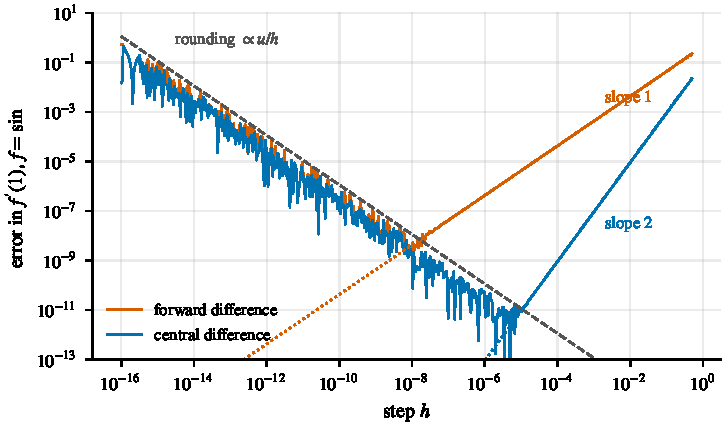
\includegraphics[width=0.85\textwidth]{fig_fd_error.pdf}
  \caption{Error of finite-difference derivatives of $\sin x$ at $x = 1$ versus step size. To the right of the optimum, truncation error
  dominates (slopes 1 and 2); to the left, rounding error grows like $u/h$. Central differences reach about $10^{-11}$; forward differences
  only about $10^{-8}$.}
  \label{fig:fd-error}
\end{figure}

\Cref{fig:fd-error} shows both error regimes. This is why the Jacobian tests of the project use central differences with $h \approx 10^{-6}$
and tolerances of about $10^{-6}$ to $10^{-8}$ relative to the size of the entries. A tolerance tighter than the achievable accuracy makes a
correct implementation fail; a much looser one lets a wrong implementation pass.

\paragraph{Jacobians.} For $f: \R^n \to \R^m$, column $j$ of the numerical Jacobian is
$\big(f(x + he_j) - f(x - he_j)\big)/2h$, costing $2n$ evaluations of $f$. On manifolds the perturbation and the difference are replaced by
$\bplus$ and $\bminus$ (\cref{ch:lie}); nothing else changes.

\begin{aside}[the complex-step derivative]
If $f$ is analytic and can be evaluated with complex arguments, $f'(x) = \operatorname{Im}f(x + ih)/h + O(h^2)$, with no subtraction at all.
With $h = 10^{-20}$ the result is exact to machine precision. The technique requires that every operation in $f$ be implemented for complex
numbers and avoid non-analytic functions (absolute values, comparisons), which rules it out for most estimator code. It is a superb way to
generate reference Jacobians in Python, though.
\end{aside}

\begin{takeaways}
\begin{itemize}
  \item The Jacobian is the matrix of the best linear approximation; the chain rule multiplies Jacobians in composition order.
  \item Taylor's theorem bounds approximation errors. ``First order'' means an error of $O(\|\delta\|^2)$.
  \item $\dd(A\inv) = -A\inv\dd A\,A\inv$ and $\dd\log\det A = \tr(A\inv\dd A)$.
  \item $\dot x = Ax + Bu$ is solved by $e^{At}$ plus a convolution of the inputs; time-varying systems use the state transition matrix,
        which is \emph{not} the exponential of the integrated system matrix unless the matrices commute.
  \item A method of order $p$ has global error $O(h^p)$; halving the step should divide the error by $2^p$. Measure it.
  \item Euler's method leaves the set of rotations; multiplicative updates $R\exp(h\sx{\omega})$ do not.
  \item Central differences with $h \approx 10^{-6}$ reach about $10^{-11}$ accuracy; forward differences only about $10^{-8}$.
\end{itemize}
\end{takeaways}

\begin{exercises}
  \item Compute the Jacobian of $f(x, y) = (x^2y, \sin(xy), e^x)$ and verify it with central differences.
  \item Use Taylor's theorem to bound the error of $\cos h \approx 1 - h^2/2$ for $|h| \le 0.1$.
  \item Show that $\nabla_x\|Ax - b\|^2 = 2A\T(Ax - b)$ and $\nabla_x^2\|Ax - b\|^2 = 2A\T A$.
  \item Solve $\dot x = -2x + 1$, $x(0) = 3$, and check the solution by substitution.
  \item For $A = \begin{bmatrix}0 & 1\\ -1 & 0\end{bmatrix}$, compute $e^{At}$ and interpret the solution of $\dot x = Ax$.
  \item Find the state transition matrix of $\dot x = \begin{bmatrix}0 & t\\0 & 0\end{bmatrix}x$. Do the matrices $A(t)$ commute?
  \item Construct two angular velocity profiles with the same integral $\int\omega\,\dd t$ that produce different final rotations.
  \item Implement Euler, Heun and RK4 for the harmonic oscillator and reproduce \cref{fig:ode-methods}(a).
  \item Show that one Euler step on $\dot R = R\sx{\omega}$ increases $\det R$ by a factor $1 + h^2\|\omega\|^2$, to leading order.
  \item Reproduce \cref{fig:fd-error} and compare the observed optimal step sizes with the formulas of \cref{sec:numdiff}.
\end{exercises}
% Solutions to the exercises of Chapter 4.
\begin{solutions}
  \item Differentiating each component with respect to $x$ and $y$,
        \[
          \frac{\partial f}{\partial(x, y)} = \begin{bmatrix} 2xy & x^2 \\ y\cos(xy) & x\cos(xy) \\ e^x & 0 \end{bmatrix}.
        \]
        At $(x, y) = (0.7, -1.3)$ this is $\begin{bmatrix}-1.82 & 0.49\\ -0.798 & 0.430\\ 2.014 & 0\end{bmatrix}$, and the central-difference Jacobian
        with $h = 10^{-6}$, column $j$ being $\big(f(x + he_j) - f(x - he_j)\big)/2h$, agrees to $10^{-10}$, the accuracy predicted in
        \cref{sec:numdiff}.

  \item The cubic Taylor term of $\cos$ at $0$ vanishes, so $1 - h^2/2$ is also the degree-3 Taylor polynomial, and \cref{thm:taylor} with $n = 3$
        gives the remainder $\cos(\xi)\,h^4/4!$. Hence $|\cos h - (1 - h^2/2)| \le h^4/24 \le 4.2\times10^{-6}$ for $|h| \le 0.1$. The bound is tight:
        at $h = 0.1$ the actual error is $4.165\times10^{-6}$. Using $n = 2$ instead would give the much weaker bound $|h|^3/6 \approx 1.7\times10^{-4}$;
        knowing which terms vanish pays off.

  \item Expand $f(x) = \|Ax - b\|^2 = x\T A\T Ax - 2b\T Ax + b\T b$. The quadratic-form rule with the symmetric matrix $A\T A$ gives
        $\nabla(x\T A\T Ax) = 2A\T Ax$, and $\nabla(b\T Ax) = A\T b$, so
        \[
          \nabla_xf = 2A\T Ax - 2A\T b = 2A\T(Ax - b), \qquad \nabla^2_xf = \frac{\partial}{\partial x}\big(2A\T Ax - 2A\T b\big) = 2A\T A .
        \]
        Setting the gradient to zero gives the normal equations; the Hessian $2A\T A \succeq 0$ shows that any such point is a minimum.

  \item With $a = -2$ and $b = 1$ the integrating-factor formula gives
        \[
          x(t) = 3e^{-2t} + \int_0^te^{-2(t-s)}\,\dd s = 3e^{-2t} + \tfrac12\big(1 - e^{-2t}\big) = \tfrac12 + \tfrac52e^{-2t}.
        \]
        Check: $\dot x = -5e^{-2t}$ and $-2x + 1 = -1 - 5e^{-2t} + 1 = -5e^{-2t}$; $x(0) = \tfrac12 + \tfrac52 = 3$. The solution decays from 3 to the
        equilibrium $\tfrac12$ with time constant $\tfrac12$.

  \item $A^2 = -I$, so as in the solution of Exercise 3.7 the series splits into the cosine and sine series:
        \[
          e^{At} = \cos t\,I + \sin t\,A = \begin{bmatrix}\cos t & \sin t\\ -\sin t & \cos t\end{bmatrix}.
        \]
        This is a rotation by $-t$. The system is $\dot x_1 = x_2$, $\dot x_2 = -x_1$, the harmonic oscillator $\ddot x_1 = -x_1$ with
        $x_1 = \text{position}$ and $x_2 = \text{velocity}$. Its solutions move clockwise around circles at unit angular rate; $\|x\|^2$, the energy, is
        conserved. (Euler's method fails to conserve it, \cref{fig:ode-methods}b.)

  \item The second equation gives $x_2(t) = x_2(s)$, and then $\dot x_1 = t\,x_2(s)$ integrates to $x_1(t) = x_1(s) + \tfrac12(t^2 - s^2)x_2(s)$, so
        \[
          \Phi(t, s) = \begin{bmatrix}1 & \tfrac12(t^2 - s^2)\\ 0 & 1\end{bmatrix}.
        \]
        The matrices do commute: $A(t)A(s) = \begin{bmatrix}0 & t\\0 & 0\end{bmatrix}\begin{bmatrix}0 & s\\0 & 0\end{bmatrix} = 0 = A(s)A(t)$.
        Accordingly property 4 of \cref{prop:stm} applies: $\int_s^tA = \begin{bmatrix}0 & \frac12(t^2 - s^2)\\0 & 0\end{bmatrix}$ is nilpotent and its
        exponential is exactly $\Phi(t, s)$.

  \item Profile A: rotate about $x$ at $\pi/2$~rad/s for one second, then about $y$ at $\pi/2$~rad/s for one second. Profile B: the same two
        segments in the opposite order. Both have $\int\omega\,\dd t = (\pi/2, \pi/2, 0)$. With body rates, $R = R(0)\exp(\cdot)\exp(\cdot)$, so the final
        rotations are
        \[
          R_A = R_x(90^\circ)R_y(90^\circ) = \begin{bmatrix}0 & 0 & 1\\ 1 & 0 & 0\\ 0 & 1 & 0\end{bmatrix}, \qquad
          R_B = R_y(90^\circ)R_x(90^\circ) = \begin{bmatrix}0 & 1 & 0\\ 0 & 0 & -1\\ -1 & 0 & 0\end{bmatrix},
        \]
        both $120^\circ$ rotations but about different axes, $120^\circ$ apart from each other. Neither equals $\exp(\sx{(\pi/2, \pi/2, 0)})$, a
        $127^\circ$ rotation about $(1, 1, 0)/\sqrt2$. The integral of $\omega$ does not determine the rotation; the order of the rotations does.

  \item The implementation follows the formulas of \cref{sec:numint}, with $f(y) = (y_2, -y_1)$, $y_0 = (1, 0)$, and $N$ steps of $h = 2\pi/N$ over one
        period:
\begin{lstlisting}[style=py]
def step(method, y, h):
    f = lambda y: np.array([y[1], -y[0]])
    if method == "Euler": return y + h * f(y)
    if method == "Heun":
        k1 = f(y); k2 = f(y + h * k1); return y + h / 2 * (k1 + k2)
    k1 = f(y); k2 = f(y + h/2 * k1); k3 = f(y + h/2 * k2); k4 = f(y + h * k3)
    return y + h / 6 * (k1 + 2 * k2 + 2 * k3 + k4)
\end{lstlisting}
        The final errors $\|y_N - y_0\|$ for $N = 32, 64, 128, 256$ are $0.84, 0.36, 0.17, 0.080$ (Euler), $4.1\times10^{-2}, 1.0\times10^{-2},
        2.5\times10^{-3}, 6.3\times10^{-4}$ (Heun) and $7.8\times10^{-5}, 4.9\times10^{-6}, 3.0\times10^{-7}, 1.9\times10^{-8}$ (RK4). The ratios between
        successive errors give measured orders $\log_2(e_h/e_{h/2}) \approx 1.1$, $2.0$ and $4.0$. Euler approaches order 1 only slowly because its
        errors are still large: at $N = 32$ the amplitude has already grown by $\big(1 + (2\pi/32)^2\big)^{16} \approx 1.8$.

  \item One Euler step is $R_{k+1} = R_k(I + h\sx{\omega})$, so $\det R_{k+1} = \det R_k\,\det(I + h\sx{\omega})$. The eigenvalues of $\sx{\omega}$ are $0$
        and $\pm i\|\omega\|$ (Exercise 2.7), so those of $I + h\sx{\omega}$ are $1$ and $1 \pm ih\|\omega\|$, and
        \[
          \det(I + h\sx{\omega}) = 1\cdot(1 + ih\|\omega\|)(1 - ih\|\omega\|) = 1 + h^2\|\omega\|^2 .
        \]
        The factor is in fact exact, not only leading order. After $n$ steps $\det R = (1 + h^2\|\omega\|^2)^n \approx e^{nh^2\|\omega\|^2}$: at 200~Hz and
        1~rad/s this is $e^{2.5\times10^{-5}\,n}$, a 2.5\% inflation per thousand steps. The Lie--Euler update $R_k\exp(h\sx{\omega})$ keeps $\det R = 1$ exactly.

  \item Evaluating the two formulas of \cref{sec:numdiff} on a log-spaced grid of $h$ for $f = \sin$ at $x = 1$ reproduces the figure. The theory
        predicts, with $u = 2^{-53}$, $|f| = \sin1 = 0.84$, $|f''| = 0.84$, $|f'''| = \cos1 = 0.54$:
        \begin{itemize}[leftmargin=1.2em]
          \item forward differences: $h^\star = 2\sqrt{u|f|/|f''|} = 2.1\times10^{-8}$, with error $2\sqrt{u|f||f''|} = 1.8\times10^{-8}$;
          \item central differences: $h^\star = (3u|f|/|f'''|)^{1/3} = 8.0\times10^{-6}$, with error $1.7\times10^{-11}$.
        \end{itemize}
        The observed minima (taking the median error in a small window of $h$, since the rounding part is erratic) lie at $h \approx 10^{-8}$ and
        $5\times10^{-6}$, with errors of about $3\times10^{-9}$ and $3\times10^{-12}$. The optimal steps agree with the formulas to within a factor of
        two, and the observed errors are a few times smaller than the predicted ones, because the formulas add worst-case rounding errors while
        the actual rounding errors of $f(x + h)$ and $f(x - h)$ are partly random and partly cancel.
\end{solutions}


\chapter{Probability and Random Vectors}
\label{ch:prob}

\begin{objectives}
\begin{itemize}
  \item Build probability from its axioms: conditional probability, independence and Bayes' rule.
  \item Work with random variables and random vectors: densities, expectations, covariances and changes of variables.
  \item Derive the Gaussian distribution and its key properties: affine maps, marginals, conditionals and the fusion of estimates.
  \item Understand the law of large numbers, the central limit theorem and Monte Carlo methods.
  \item Derive the $\chi^2$ distribution and use it for hypothesis tests, the basis of gating and consistency checks.
  \item Understand how nonlinear functions distort distributions, and what linearization keeps and loses.
\end{itemize}
\end{objectives}

A filter does not merely estimate the state; it maintains a probability distribution over it. The estimate is the center of
that distribution, and the covariance describes its spread. This chapter develops the probability theory that gives these words a
precise meaning.

% ==============================================================================
\section{Probability}

\subsection{Events and the axioms}

A random experiment has a set $\Omega$ of possible outcomes, the \term{sample space}. An \term{event} is a subset of outcomes, and a
\term{probability} assigns to each event $A$ a number $P(A)$ obeying three axioms (Kolmogorov):
\begin{enumerate}
  \item $P(A) \ge 0$ for every event;
  \item $P(\Omega) = 1$;
  \item if $A_1, A_2, \dots$ are mutually exclusive (pairwise disjoint), $P(A_1\cup A_2\cup\cdots) = \sum_iP(A_i)$.
\end{enumerate}
Everything else follows: $P(\text{not }A) = 1 - P(A)$, $P(A\cup B) = P(A) + P(B) - P(A\cap B)$, and so on. Probability can be read as a
long-run frequency (the fraction of repetitions in which $A$ occurs) or as a degree of belief; the mathematics is the same, and filters
use both readings.

\subsection{Conditional probability and independence}

\begin{definition}[Conditional probability]
For $P(B) > 0$, the probability of $A$ given $B$ is $P(A\mid B) = P(A\cap B)/P(B)$.
\end{definition}

Conditioning restricts attention to the outcomes in which $B$ happened and renormalizes. Two events are \term{independent} if
$P(A\cap B) = P(A)P(B)$, equivalently $P(A\mid B) = P(A)$: knowing that $B$ occurred tells nothing about $A$.

\begin{proposition}[Law of total probability and Bayes' rule]
\index{Bayes' rule}
If $B_1, \dots, B_n$ are mutually exclusive and cover $\Omega$, then $P(A) = \sum_iP(A\mid B_i)P(B_i)$, and
\begin{equation}
  P(B_i\mid A) = \frac{P(A\mid B_i)\,P(B_i)}{\sum_jP(A\mid B_j)\,P(B_j)} .
\end{equation}
\end{proposition}
\begin{proof}
$A$ is the disjoint union of the $A\cap B_i$, and $P(A\cap B_i) = P(A\mid B_i)P(B_i)$. Bayes' rule is the definition of conditional
probability applied twice: $P(B_i\mid A)P(A) = P(A\cap B_i) = P(A\mid B_i)P(B_i)$.
\end{proof}

Bayes' rule turns the probability of an observation given a hypothesis (which a sensor model provides) into the probability of the
hypothesis given the observation (which we want).

\begin{worked}[how informative is a passed test?]
Suppose 10\% of the feature tracks reaching an outlier test are wrong. The test rejects 90\% of wrong tracks, and (being a 95\% gate)
also rejects 5\% of correct ones. A track passes. What is the probability that it is wrong? With $W$ = ``wrong'' and $A$ = ``passes'':
$P(A\mid W) = 0.1$, $P(W) = 0.1$, $P(A\mid\text{correct}) = 0.95$, $P(\text{correct}) = 0.9$. Bayes' rule gives
\begin{equation*}
  P(W\mid A) = \frac{0.1\times0.1}{0.1\times0.1 + 0.95\times0.9} = \frac{0.01}{0.865} \approx 1.2\% .
\end{equation*}
The test reduces the outlier fraction from 10\% to about 1\%: very useful, but not perfect, which is why the estimator adds further
checks downstream.
\end{worked}

% ==============================================================================
\section{Random variables}

\subsection{Distributions, densities and expectations}

A \term{random variable} $X$ is a numerical quantity determined by the outcome of an experiment. Its \emph{cumulative distribution
function} is $F(x) = P(X \le x)$. A discrete random variable takes countably many values with probabilities $p(x) = P(X = x)$; a continuous
one has a \term{probability density function} (pdf) $p(x) \ge 0$ with
\begin{equation}
  P(a \le X \le b) = \int_a^bp(x)\,\dd x, \qquad \int_{-\infty}^\infty p(x)\,\dd x = 1 .
\end{equation}
A density is not a probability: $p(x)\,\dd x$ is the probability of falling in a small interval of width $\dd x$ around $x$, and a density
can exceed one.

\begin{definition}[Expectation and variance]
The \term{expectation} (mean) of $X$ is $\E[X] = \int x\,p(x)\,\dd x$ (a sum for discrete variables). The expectation of a function of $X$ is
$\E[g(X)] = \int g(x)p(x)\,\dd x$. The \term{variance} is $\Var(X) = \E[(X - \E X)^2] = \E[X^2] - (\E X)^2$, and its square root is the
\term{standard deviation} $\sigma$.
\end{definition}

Expectation is linear: $\E[aX + bY + c] = a\E[X] + b\E[Y] + c$ for any random variables, dependent or not. Variance scales quadratically and
ignores shifts: $\Var(aX + c) = a^2\Var(X)$. The standard deviation has the units of $X$ and measures its typical spread.

\begin{example}[Uniform distribution]
$X$ uniform on $[a, b]$ has $p(x) = 1/(b - a)$ there, mean $(a + b)/2$ and variance $(b - a)^2/12$. Rounding a reading to a resolution
$\Delta$ produces an error that is approximately uniform on $[-\Delta/2, \Delta/2]$, with standard deviation $\Delta/\sqrt{12}$: the
quantization noise of a sensor.
\end{example}

\subsection{The Gaussian distribution}

\begin{definition}[Gaussian distribution]
\index{Gaussian distribution}
$X \sim \N(\mu, \sigma^2)$ has density
\begin{equation}
  p(x) = \frac{1}{\sqrt{2\pi}\,\sigma}\exp\!\Big(-\frac{(x - \mu)^2}{2\sigma^2}\Big).
\end{equation}
The \emph{standard normal} distribution is $\N(0, 1)$.
\end{definition}

\begin{proposition}[Normalization]
$\int_{-\infty}^\infty e^{-x^2/2}\,\dd x = \sqrt{2\pi}$.
\end{proposition}
\begin{proof}
Let $I$ be the integral. Then $I^2 = \iint e^{-(x^2 + y^2)/2}\,\dd x\,\dd y$. In polar coordinates, with area element $r\,\dd r\,\dd\theta$,
$I^2 = \int_0^{2\pi}\!\int_0^\infty e^{-r^2/2}r\,\dd r\,\dd\theta = 2\pi\big[-e^{-r^2/2}\big]_0^\infty = 2\pi$.
\end{proof}

Substituting $x \to (x - \mu)/\sigma$ shows that the general density integrates to one, and similar integrals (using symmetry and
integration by parts) give $\E[X] = \mu$ and $\Var(X) = \sigma^2$. If $X \sim \N(\mu, \sigma^2)$ then $(X - \mu)/\sigma \sim \N(0, 1)$, and the
probabilities of falling within one, two and three standard deviations of the mean are $68.27\%$, $95.45\%$ and $99.73\%$. A Gaussian is
completely determined by its mean and variance, and is closed under the operations a linear filter performs, which is why Kalman
filters can work with means and covariances alone.

% ==============================================================================
\section{Several random variables}

\subsection{Joint, marginal and conditional densities}

Two random variables $X, Y$ have a \emph{joint density} $p(x, y)$, with $P((X, Y) \in A) = \iint_Ap(x, y)\,\dd x\,\dd y$. From it:
\begin{align}
  \text{marginal:}&\quad p(x) = \int p(x, y)\,\dd y, \\
  \text{conditional:}&\quad p(x\mid y) = \frac{p(x, y)}{p(y)}, \\
  \text{Bayes' rule:}&\quad p(x\mid y) = \frac{p(y\mid x)\,p(x)}{p(y)} = \frac{p(y\mid x)\,p(x)}{\int p(y\mid x')p(x')\,\dd x'} .
\end{align}
$X$ and $Y$ are independent if $p(x, y) = p(x)p(y)$. In estimation, $x$ is the unknown state and $y$ the measurement: $p(y\mid x)$ is the
sensor model (the \emph{likelihood}), $p(x)$ is the \emph{prior}, and $p(x\mid y)$ the \emph{posterior}.

\subsection{Covariance and correlation}

The \term{covariance} $\Cov(X, Y) = \E[(X - \E X)(Y - \E Y)]$ measures how two variables vary together, and the \term{correlation
coefficient} $\rho = \Cov(X, Y)/(\sigma_X\sigma_Y) \in [-1, 1]$ normalizes it (the bound is the Cauchy--Schwarz inequality). Independent
variables have zero covariance, and then $\Var(X + Y) = \Var(X) + \Var(Y)$: variances of independent errors add.

The converse fails: zero correlation does not imply independence. If $X \sim \N(0, 1)$ and $Y = X^2$, then $\Cov(X, Y) = \E[X^3] = 0$, yet $Y$
is a function of $X$. Correlation measures only \emph{linear} dependence. (For jointly Gaussian variables the converse does hold, as shown
below.)

% ==============================================================================
\section{Random vectors}

\subsection{Mean and covariance}

For a random vector $x \in \R^n$ with density $p(x)$, the mean and \term{covariance matrix} are
\begin{equation}
  \mu = \E[x], \qquad \Sigma = \Cov(x) = \E\big[(x - \mu)(x - \mu)\T\big] = \E[xx\T] - \mu\mu\T .
\end{equation}
The diagonal of $\Sigma$ holds the variances $\sigma_i^2$ and its off-diagonal entries the covariances. $\Sigma$ is symmetric and positive
semi-definite: for any fixed $a$, $a\T\Sigma a = \E\big[(a\T(x - \mu))^2\big] \ge 0$. The \emph{cross-covariance} of two random vectors is
$\Sigma_{xy} = \E[(x - \mu_x)(y - \mu_y)\T]$, and $\Sigma_{yx} = \Sigma_{xy}\T$.

\begin{proposition}[Affine transformations]
\label{prop:affine}
If $y = Ax + b$ then $\E[y] = A\mu + b$ and $\Cov(y) = A\Sigma A\T$. If $x$ and $w$ are uncorrelated, $\Cov(Ax + Bw) = A\Sigma_xA\T + B\Sigma_wB\T$.
\end{proposition}
\begin{proof}
Linearity of expectation gives the mean. Then $\Cov(y) = \E[A(x - \mu)(x - \mu)\T A\T] = A\Sigma A\T$. With uncorrelated $x$ and $w$, the cross terms
$A\Sigma_{xw}B\T$ vanish.
\end{proof}

This one proposition is the covariance propagation of the Kalman filter ($P \leftarrow \Phi P \Phi\T + Q$), the covariance of a stacked
measurement, and the augmentation formula of stochastic cloning ($P \leftarrow JPJ\T$).

\begin{proposition}[Expected value of a quadratic form]
\label{prop:quadratic-expectation}
For any matrix $A$, $\E[x\T Ax] = \tr(A\Sigma) + \mu\T A\mu$. In particular, if $\mu = 0$ then $\E[x\T\Sigma\inv x] = \tr(I_n) = n$.
\end{proposition}
\begin{proof}
$x\T Ax = \tr(Axx\T)$, and expectation commutes with the trace: $\E[x\T Ax] = \tr(A\,\E[xx\T]) = \tr(A(\Sigma + \mu\mu\T))$.
\end{proof}

The special case is the reason a consistent filter's normalized estimation error squared averages to the dimension of the state
(\cref{ch:consistency}).

\subsection{Changing variables}

\begin{proposition}[Change of variables]
\label{prop:change-of-variables}
If $y = g(x)$ with $g$ invertible and differentiable, the densities are related by
$p_y(y) = p_x\big(g\inv(y)\big)\,\big|\det\frac{\partial g\inv}{\partial y}\big|$.
\end{proposition}

In one dimension this follows from equating probabilities of corresponding small intervals, $p_y(y)\,|\dd y| = p_x(x)\,|\dd x|$; in several
dimensions the determinant measures how $g\inv$ stretches volumes (\cref{sec:determinants}). For an invertible linear map $y = Ax$ the factor
is the constant $1/|\det A|$.

% ==============================================================================
\section{The multivariate Gaussian}

\subsection{Definition}

\begin{definition}[Multivariate Gaussian]
\index{Gaussian distribution!multivariate}
A random vector $x \in \R^n$ is Gaussian, $x \sim \N(\mu, \Sigma)$, if it can be written as $x = \mu + Ls$ where $s$ has independent standard
normal components and $LL\T = \Sigma$. If $\Sigma \succ 0$ its density is
\begin{equation}
  p(x) = \frac{1}{\sqrt{(2\pi)^n \det\Sigma}}\exp\!\Big( -\tfrac12 (x - \mu)\T \Sigma\inv (x - \mu) \Big).
  \label{eq:gaussian-pdf}
\end{equation}
The quantity $d_M^2(x) = (x - \mu)\T\Sigma\inv(x - \mu)$ is the squared \term{Mahalanobis distance} of $x$ from the mean.
\end{definition}

\begin{proof}[Derivation of the density]
The density of $s$ is the product of $n$ standard normal densities, $(2\pi)^{-n/2}\exp(-\tfrac12s\T s)$. By \cref{prop:change-of-variables} with
$s = L\inv(x - \mu)$, $p(x) = (2\pi)^{-n/2}\exp\big(-\tfrac12(x - \mu)\T L\mT L\inv(x - \mu)\big)/|\det L|$. Since $L\mT L\inv = (LL\T)\inv = \Sigma\inv$ and
$|\det L| = \sqrt{\det\Sigma}$, this is \eqref{eq:gaussian-pdf}.
\end{proof}

By \cref{prop:affine}, the mean of $x$ is $\mu$ and its covariance is $L\,\E[ss\T]L\T = \Sigma$. The definition also handles singular
covariances (with $L$ not invertible), which arise naturally in stochastic cloning (\cref{ch:cloning}).

\begin{figure}[t]
  \centering
  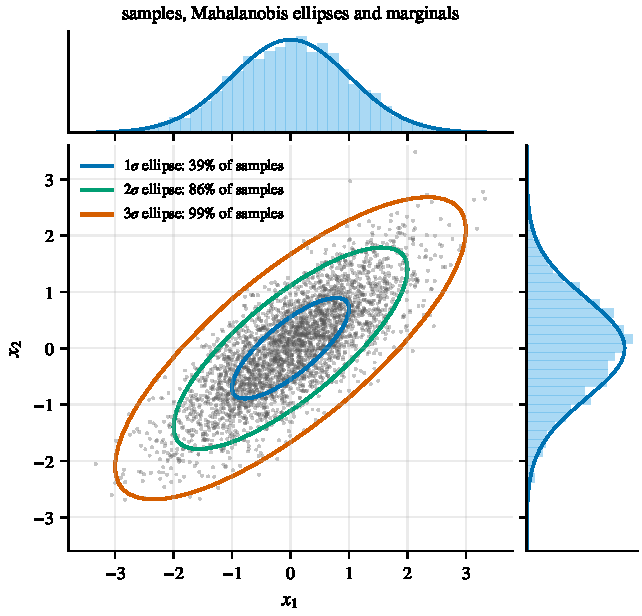
\includegraphics[width=0.92\textwidth]{fig_gauss2d.pdf}
  \caption{Samples of a correlated 2D Gaussian with the $1\sigma$, $2\sigma$ and $3\sigma$ Mahalanobis ellipses, and the two marginal densities.
  The ellipses are aligned with the eigenvectors of $\Sigma$. In two dimensions they contain 39\%, 86\% and 99\% of the probability, not
  the familiar 68--95--99.7\% of one dimension.}
  \label{fig:gauss2d}
\end{figure}

\paragraph{Geometry.} The density is constant on the ellipsoids $d_M^2(x) = c$, whose axes point along the eigenvectors of $\Sigma$ with lengths
proportional to the square roots of its eigenvalues (\cref{fig:ellipse,fig:gauss2d}). The Mahalanobis distance measures distance in units of
standard deviations along each principal axis, which makes it the natural way to ask whether a vector is ``far'' from a distribution.

\paragraph{Sampling.} To draw from $\N(\mu, \Sigma)$, factor $\Sigma = LL\T$ (Cholesky), draw $s \sim \N(0, I)$, and return $\mu + Ls$. Monte Carlo tests
of covariance propagation (Milestone 5) use exactly this.

\paragraph{Closure.} Affine maps of Gaussian vectors are Gaussian (directly from the definition). Marginals, conditionals and products of
Gaussian densities are Gaussian (next section). Hence a Gaussian belief propagated through a linear system with Gaussian noise remains
exactly Gaussian, and the Kalman filter is exact in that case. For jointly Gaussian vectors, uncorrelated implies independent: if the
covariance is block diagonal, the density factors.

\paragraph{Information form.} A Gaussian can equally be parameterized by the \term{information matrix} $\Lambda = \Sigma\inv$ and the
\emph{information vector} $\eta = \Sigma\inv\mu$. Then $-\log p(x) = \tfrac12 x\T\Lambda x - \eta\T x + \text{const}$. The information form is natural
for combining independent pieces of evidence, since their information adds, and it is the form in which optimization-based estimators work.

\subsection{Marginals and conditionals}

Partition a jointly Gaussian vector as
\begin{equation}
  \begin{bmatrix} a \\ b \end{bmatrix} \sim
  \N\!\left( \begin{bmatrix} \mu_a \\ \mu_b \end{bmatrix},
  \begin{bmatrix} \Sigma_{aa} & \Sigma_{ab} \\ \Sigma_{ba} & \Sigma_{bb} \end{bmatrix} \right),
  \qquad
  \Lambda = \Sigma\inv = \begin{bmatrix} \Lambda_{aa} & \Lambda_{ab} \\ \Lambda_{ba} & \Lambda_{bb} \end{bmatrix}.
\end{equation}

\begin{theorem}[Gaussian marginalization and conditioning]
\label{thm:gauss-cond}
\index{marginalization}\index{conditioning}
\begin{enumerate}
  \item The marginal of $a$ is $\N(\mu_a, \Sigma_{aa})$.
  \item The conditional of $a$ given $b$ is $\N(\mu_{a|b}, \Sigma_{a|b})$ with
  \begin{equation}
    \mu_{a|b} = \mu_a + \Sigma_{ab}\Sigma_{bb}\inv (b - \mu_b), \qquad
    \Sigma_{a|b} = \Sigma_{aa} - \Sigma_{ab}\Sigma_{bb}\inv\Sigma_{ba}.
    \label{eq:gauss-cond}
  \end{equation}
\end{enumerate}
\end{theorem}
\begin{proof}
The marginal follows from \cref{prop:affine} with the selection matrix $A = [I\ \ 0]$. For the conditional, define
$\tilde a = a - \Sigma_{ab}\Sigma_{bb}\inv b$. Then $\Cov(\tilde a, b) = \Sigma_{ab} - \Sigma_{ab}\Sigma_{bb}\inv\Sigma_{bb} = 0$, so $\tilde a$ and $b$ are uncorrelated,
and being jointly Gaussian they are independent. By \cref{prop:affine},
$\tilde a \sim \N(\mu_a - \Sigma_{ab}\Sigma_{bb}\inv\mu_b,\ \Sigma_{aa} - \Sigma_{ab}\Sigma_{bb}\inv\Sigma_{ba})$. Conditioning on $b$ leaves the distribution of
$\tilde a$ unchanged (independence), and $a = \tilde a + \Sigma_{ab}\Sigma_{bb}\inv b$, which gives \eqref{eq:gauss-cond}.
\end{proof}

The conditional mean moves away from $\mu_a$ in proportion to how far $b$ is from its mean, by the ``regression'' matrix $\Sigma_{ab}\Sigma_{bb}\inv$,
and the conditional covariance shrinks by a positive semi-definite amount. It does not depend on the observed value of $b$, only on the
fact that it was observed. The conditional covariance is the Schur complement $\Sigma/\Sigma_{bb}$; applying \cref{prop:block-inverse} to $\Sigma$
shows that $\Lambda_{aa} = \Sigma_{a|b}\inv$ and that the marginal information matrix is a Schur complement of $\Lambda$. The two parameterizations
therefore swap the roles of the two operations:

\begin{center}\small
\begin{tabular}{@{}lll@{}}
\toprule
 & covariance form $(\mu, \Sigma)$ & information form $(\eta, \Lambda)$ \\
\midrule
marginalize out $b$ & $\Sigma_{aa}$ \hfill(\textbf{delete rows/columns}) & $\Lambda_{aa} - \Lambda_{ab}\Lambda_{bb}\inv\Lambda_{ba}$ \hfill(Schur compl.) \\
condition on $b$ & $\Sigma_{aa} - \Sigma_{ab}\Sigma_{bb}\inv\Sigma_{ba}$ \hfill(Schur compl.) & $\Lambda_{aa}$ \hfill(\textbf{delete rows/columns}) \\
\bottomrule
\end{tabular}
\end{center}

\begin{keyidea}[marginalization is free in covariance form]
A Kalman filter stores covariances, so discarding a variable (the oldest clone of the MSCKF window) is literally deleting its rows and
columns from $P$. Optimization-based estimators store information matrices, so the same operation requires a Schur complement, which
creates fill-in and the ``marginalization prior'' of sliding-window smoothers (\cref{ch:nlls}).
\end{keyidea}

% ==============================================================================
\section{Fusing information: Bayes' rule for Gaussians}

\subsection{Combining two estimates}

Suppose two independent sensors measure the same scalar $x$, with readings $z_1 = x + n_1$ and $z_2 = x + n_2$ and noise variances $\sigma_1^2$ and
$\sigma_2^2$. With no other knowledge of $x$, the posterior density is proportional to the product of the two likelihoods,
\begin{equation}
  p(x\mid z_1, z_2) \propto \exp\!\Big(-\frac{(x - z_1)^2}{2\sigma_1^2}\Big)\exp\!\Big(-\frac{(x - z_2)^2}{2\sigma_2^2}\Big).
\end{equation}
The exponent is a quadratic in $x$; completing the square shows that the posterior is Gaussian with
\begin{equation}
  \frac{1}{\sigma^2} = \frac1{\sigma_1^2} + \frac1{\sigma_2^2}, \qquad
  \hat x = \sigma^2\Big(\frac{z_1}{\sigma_1^2} + \frac{z_2}{\sigma_2^2}\Big) = z_1 + \frac{\sigma_1^2}{\sigma_1^2 + \sigma_2^2}(z_2 - z_1).
  \label{eq:fusion}
\end{equation}
\emph{Inverse variances (information) add}, and the fused estimate is an information-weighted average. The second form already has the shape
of a Kalman update: start from $z_1$ and correct it by a gain times the discrepancy $z_2 - z_1$, with a gain between 0 and 1 that is large
when the first estimate is poor. The fused variance is smaller than both, so combining independent information always helps.

\subsection{The linear-Gaussian model}

\begin{proposition}[Linear-Gaussian posterior]
\label{prop:map-ls}
If $x \sim \N(\mu, P)$ and $z = Hx + n$ with $n \sim \N(0, R)$ independent of $x$, the posterior $p(x\mid z)$ is Gaussian, and its mean (which is
also its mode) solves the weighted least-squares problem
\begin{equation}
  \hat x = \argmin_x\ \|x - \mu\|^2_{P\inv} + \|z - Hx\|^2_{R\inv},
  \qquad \|e\|^2_{W} := e\T W e .
  \label{eq:map-ls}
\end{equation}
Its covariance is $(P\inv + H\T R\inv H)\inv$.
\end{proposition}
\begin{proof}
By Bayes' rule $p(x\mid z) \propto p(z\mid x)p(x)$, and
$-\log p(x\mid z) = \tfrac12\|x - \mu\|^2_{P\inv} + \tfrac12\|z - Hx\|^2_{R\inv} + \text{const}$. This is a convex quadratic in $x$ whose quadratic term is
$\tfrac12x\T(P\inv + H\T R\inv H)x$, so the posterior is Gaussian with that information matrix, and its mode, which for a Gaussian is the mean,
minimizes the quadratic.
\end{proof}

This is the scalar fusion rule in matrix form: the prior contributes information $P\inv$, the measurement contributes $H\T R\inv H$, and they add.
\Cref{ch:estimation} develops this into the general theory of estimators, and \cref{ch:kf} turns it into the Kalman filter.

% ==============================================================================
\section{Limit theorems and Monte Carlo}

\subsection{The law of large numbers}

Let $X_1, X_2, \dots$ be independent draws from the same distribution, with mean $\mu$ and variance $\sigma^2$, and let
$\bar X_N = \frac1N\sum_{i=1}^NX_i$ be their \term{sample mean}. Then $\E[\bar X_N] = \mu$ and, because variances of independent terms add,
$\Var(\bar X_N) = \sigma^2/N$.

\begin{theorem}[Weak law of large numbers]
\index{law of large numbers}
For every $\epsilon > 0$, $P(|\bar X_N - \mu| > \epsilon) \to 0$ as $N\to\infty$.
\end{theorem}
\begin{proof}
Chebyshev's inequality $P(|Y - \E Y| \ge \epsilon) \le \Var(Y)/\epsilon^2$ (which follows from
$\Var(Y) \ge \E[(Y - \E Y)^2\,\mathbf 1_{|Y - \E Y|\ge\epsilon}] \ge \epsilon^2P(|Y - \E Y|\ge\epsilon)$) applied to $\bar X_N$ gives the bound
$\sigma^2/(N\epsilon^2) \to 0$.
\end{proof}

The law of large numbers justifies \term{Monte Carlo} methods: to estimate an expectation, average many independent samples. The error
shrinks only like $\sigma/\sqrt N$, so each additional digit of accuracy costs a hundred times more samples.

\subsection{The central limit theorem}

\begin{theorem}[Central limit theorem]
\index{central limit theorem}
Under the same assumptions, the distribution of $\sqrt N(\bar X_N - \mu)/\sigma$ converges to $\N(0, 1)$.
\end{theorem}

\begin{figure}[t]
  \centering
  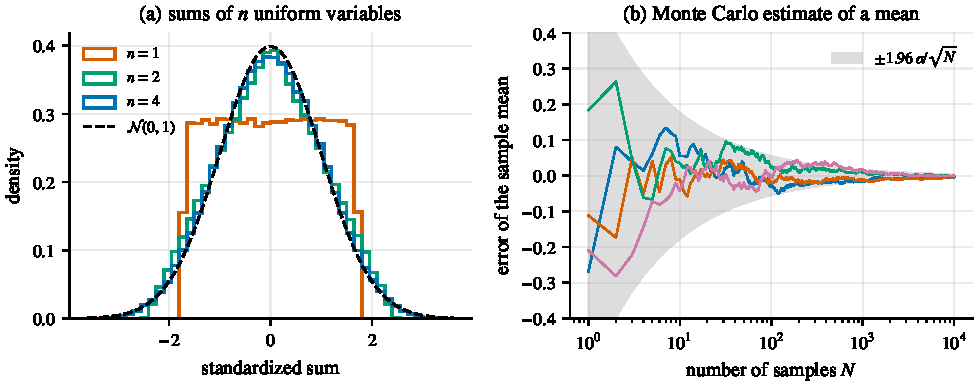
\includegraphics[width=\textwidth]{fig_clt.pdf}
  \caption{(a) The central limit theorem: histograms of the standardized sum of $n$ independent uniform variables approach the standard normal
  density already for $n = 4$. (b) Monte Carlo estimation of a mean: the error of the sample mean shrinks like $1/\sqrt N$ (gray band:
  $\pm1.96\,\sigma/\sqrt N$, the 95\% interval).}
  \label{fig:clt}
\end{figure}

Sums of many small independent effects are approximately Gaussian, whatever the distribution of each effect (\cref{fig:clt}). Electronic
sensor noise is the sum of many microscopic fluctuations, and integrating a noisy signal sums many samples; both are why Gaussian noise
models work well in navigation. They work less well for rare large errors (outliers), which is why estimators also need gating and robust
methods (\cref{ch:updates,ch:nlls}).

% ==============================================================================
\section{The chi-squared distribution}
\label{sec:chi2}

\begin{definition}
\index{chi-squared distribution}
If $s_1, \dots, s_k$ are independent standard normal variables, $\gamma = \sum_{i=1}^k s_i^2$ has the $\chi^2$ distribution with $k$ degrees of freedom,
written $\gamma \sim \chi^2_k$.
\end{definition}

\begin{proposition}[Properties of $\chi^2_k$]
$\E[\gamma] = k$ and $\Var(\gamma) = 2k$. Its density is
\begin{equation}
  p(\gamma) = \frac{\gamma^{k/2 - 1}e^{-\gamma/2}}{2^{k/2}\,\Gamma(k/2)}, \qquad \gamma > 0,
\end{equation}
where $\Gamma$ is the gamma function ($\Gamma(m) = (m - 1)!$ for integers, $\Gamma(\tfrac12) = \sqrt\pi$).
\end{proposition}
\begin{proof}[Proof of the moments and of the case $k = 1$]
For $s \sim \N(0, 1)$, $\E[s^2] = 1$ and $\E[s^4] = 3$ (integration by parts), so $\Var(s^2) = 2$; the moments of the sum follow by additivity
over independent terms. For $k = 1$, $\gamma = s^2$ takes the value $\gamma$ when $s = \pm\sqrt\gamma$, so
$p(\gamma) = 2\cdot\frac{1}{\sqrt{2\pi}}e^{-\gamma/2}\cdot\frac{\dd\sqrt\gamma}{\dd\gamma} = \frac{1}{\sqrt{2\pi\gamma}}e^{-\gamma/2}$, which is the formula with $k = 1$.
The general case follows by convolving densities (or by integrating the Gaussian density over spherical shells).
\end{proof}

\begin{theorem}[Mahalanobis distance of a Gaussian]
\label{thm:mahalanobis-chi2}
If $x \sim \N(\mu, \Sigma)$ in $\R^k$ with $\Sigma \succ 0$, then $(x-\mu)\T\Sigma\inv(x - \mu) \sim \chi^2_k$.
\end{theorem}
\begin{proof}
With $\Sigma = LL\T$, the whitened vector $s = L\inv(x - \mu)$ is $\N(0, I)$ by \cref{prop:affine}, and $(x - \mu)\T\Sigma\inv(x-\mu) = s\T s = \sum_is_i^2$.
\end{proof}

\begin{figure}[t]
  \centering
  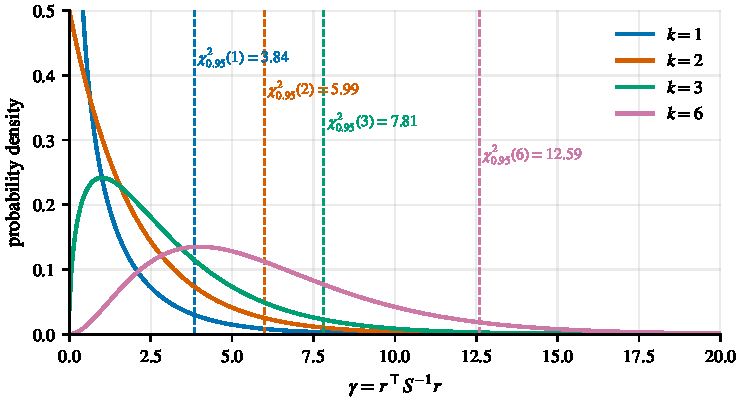
\includegraphics[width=0.84\textwidth]{fig_chi2.pdf}
  \caption{$\chi^2$ densities and their 95\% quantiles. A 2D image measurement whose normalized innovation squared exceeds $5.99$ would occur by
  chance only 5\% of the time if the filter's covariance were correct.}
  \label{fig:chi2}
\end{figure}

The \emph{quantile} $\chi^2_p(k)$ is the value below which a $\chi^2_k$ variable falls with probability $p$ (\cref{fig:chi2}; tables in
\cref{app:tables}). Because independent $\chi^2$ variables add, with their degrees of freedom adding, the sum of $N$ independent squared
Mahalanobis distances of $n$-dimensional Gaussians is $\chi^2_{Nn}$. As $k$ grows, $\chi^2_k$ is approximately $\N(k, 2k)$, so its quantiles approach
$k \pm 1.96\sqrt{2k}$.

% ==============================================================================
\section{Sample statistics and hypothesis tests}

\subsection{Estimating a mean and a variance}

Given independent samples $X_1, \dots, X_N$ of a distribution with unknown mean and variance, the natural estimates are the sample mean
$\bar X$ and the \term{sample variance}
\begin{equation}
  s^2 = \frac{1}{N - 1}\sum_{i=1}^N(X_i - \bar X)^2 .
\end{equation}
The divisor $N - 1$ makes $s^2$ unbiased. Expanding, $\sum_i(X_i - \bar X)^2 = \sum_i(X_i - \mu)^2 - N(\bar X - \mu)^2$, whose expectation is
$N\sigma^2 - N\cdot\sigma^2/N = (N - 1)\sigma^2$: one degree of freedom is used up by estimating the mean. For Gaussian samples one can show
moreover that $(N - 1)s^2/\sigma^2 \sim \chi^2_{N-1}$. This gives exact acceptance intervals for comparing a Monte Carlo sample variance with a
predicted variance, as Milestone 5 requires: the ratio $s^2/\sigma^2$ should lie between $\chi^2_{0.025}(N-1)/(N-1)$ and $\chi^2_{0.975}(N-1)/(N-1)$
95\% of the time (for $N = 500$, between $0.880$ and $1.128$; \cref{app:tables}).

\subsection{Hypothesis testing}

A \term{hypothesis test} decides whether data are compatible with a model. The recipe:
\begin{enumerate}
  \item State a \emph{null hypothesis} $H_0$, for example ``this measurement is consistent with the filter's prediction''.
  \item Choose a \emph{test statistic} whose distribution under $H_0$ is known, for example the squared Mahalanobis distance of the
        innovation, which is $\chi^2_m$ under $H_0$.
  \item Choose a \emph{significance level} $\alpha$ (often 5\%) and an \emph{acceptance region} that contains the statistic with probability
        $1 - \alpha$ under $H_0$.
  \item Reject $H_0$ if the statistic falls outside the region.
\end{enumerate}
Two errors are possible. A \emph{type I error} rejects a true $H_0$; by construction it happens with probability $\alpha$. A \emph{type II
error} accepts a false $H_0$; its probability depends on how different the truth is from $H_0$, and one minus it is the \emph{power} of the
test. Lowering $\alpha$ reduces false rejections at the price of more missed detections.

\emph{One-sided} tests reject only large values. Measurement gating is one-sided: a measurement is rejected when its Mahalanobis distance
exceeds $\chi^2_{1-\alpha}(m)$, because only large innovations indicate outliers (\cref{ch:updates}). \emph{Two-sided} tests reject both
unusually large and unusually small values. Filter consistency tests are two-sided: an average normalized error that is too small reveals an
underconfident filter just as one that is too large reveals an overconfident one (\cref{ch:consistency}).

\begin{pitfall}[a 5\% test rejects 5\% of good data]
At a 95\% gate, one in twenty perfectly good measurements is rejected. Over thousands of measurements this is expected and harmless,
provided rejections are counted. A rejection rate far from the design value is itself a symptom worth investigating.
\end{pitfall}

% ==============================================================================
\section{Nonlinear transformations}
\label{sec:linearization}

If $y = f(x)$ with $f$ nonlinear and $x \sim \N(\mu, \Sigma)$, then $y$ is generally \emph{not} Gaussian. The extended Kalman filter approximates it
by a Gaussian, linearizing $f$ about the mean:
\begin{equation}
  y \approx f(\mu) + J(x - \mu), \quad J = \frac{\partial f}{\partial x}\Big|_{\mu}
  \qquad\Longrightarrow\qquad
  y \mathrel{\dot\sim} \N\big(f(\mu),\ J\Sigma J\T\big).
\end{equation}
How much does this miss? In one dimension, Taylor expansion to second order gives
$f(x) \approx f(\mu) + f'(\mu)(x - \mu) + \tfrac12f''(\mu)(x - \mu)^2$, and taking expectations,
\begin{equation}
  \E[f(x)] \approx f(\mu) + \tfrac12f''(\mu)\,\sigma^2 .
\end{equation}
Linearization therefore ignores a \emph{bias} proportional to the curvature times the variance. The approximation is good when $f$ is nearly
linear over the region where $x$ has most of its probability mass, a few standard deviations around $\mu$.

\begin{figure}[t]
  \centering
  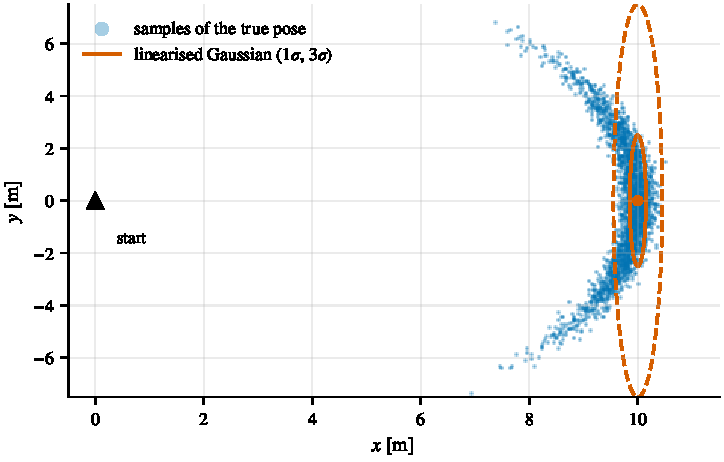
\includegraphics[width=0.84\textwidth]{fig_banana.pdf}
  \caption{A robot drives 10~m with a heading uncertainty of $\sigma_\psi = 0.25$~rad. The true distribution of its final position (samples) is a
  curved ``banana''. The linearized Gaussian (ellipses) matches its first two moments only locally, puts probability where the robot cannot be,
  and misses the curvature. Errors of this kind are why an estimator must keep its errors small, the central design principle of the
  error-state filter.}
  \label{fig:banana}
\end{figure}

\Cref{fig:banana} shows a classic failure. When heading uncertainty is large, positions are distributed along an arc, and the linearized Gaussian
is a poor description: its mean lies outside the arc, and it assigns probability to positions the robot cannot reach. Two remedies exist.
One is to reduce the uncertainty that must be linearized: the error-state filter of \cref{ch:eskf} keeps the estimation error, not the state,
as the quantity it linearizes, and continually resets it to zero. The other is to choose coordinates in which the distribution is close to
Gaussian: a Gaussian on the heading angle and travelled distance, pushed through the exact kinematics, reproduces the banana. \Cref{ch:lie}
develops that idea for rotations, and \cref{ch:nonlinear} presents a third remedy, sigma-point methods that propagate a few carefully chosen
samples instead of a linearization.

\begin{takeaways}
\begin{itemize}
  \item Bayes' rule converts a sensor model $p(z\mid x)$ and a prior $p(x)$ into the posterior $p(x\mid z)$.
  \item Affine maps propagate covariances as $A\Sigma A\T$. This single fact drives prediction, cloning and stacking.
  \item $\E[x\T Ax] = \tr(A\Sigma) + \mu\T A\mu$; the normalized squared error of an $n$-dimensional Gaussian averages to $n$.
  \item In covariance form, marginalization deletes rows and columns and conditioning takes a Schur complement. Information form is the reverse.
  \item Fusing independent Gaussian information adds inverse covariances; the result is a gain-weighted correction.
  \item Monte Carlo errors shrink like $1/\sqrt N$; sums of many small effects are nearly Gaussian.
  \item The squared Mahalanobis distance of an $n$-dimensional Gaussian is $\chi^2_n$: the basis of gating and consistency tests.
  \item Linearization ignores curvature-induced bias and fails when uncertainty is large relative to curvature.
\end{itemize}
\end{takeaways}

\begin{exercises}
  \item A gyro is either healthy (99\%) or faulty (1\%). A self-test flags 98\% of faulty units and 3\% of healthy ones. A unit is flagged; what is
        the probability that it is faulty?
  \item Let $x \sim \N(0, \diag(1, 4))$ and $y = Ax$ with $A$ a rotation by $30^\circ$. Compute $\Cov(y)$ and sketch the $1\sigma$ ellipses of $x$ and $y$.
  \item Prove that $\Sigma_{a|b} \preceq \Sigma_{aa}$: conditioning never increases uncertainty in the Loewner order. When is the inequality an equality?
  \item Derive the information-form marginal $\Lambda_{aa} - \Lambda_{ab}\Lambda_{bb}\inv\Lambda_{ba}$ from \cref{prop:block-inverse} and show that it equals $\Sigma_{aa}\inv$.
  \item Complete the square to derive \eqref{eq:fusion}.
  \item Solve \eqref{eq:map-ls} by setting the gradient to zero, and show that the solution can be written $\hat x = \mu + K(z - H\mu)$ for
        $K = (P\inv + H\T R\inv H)\inv H\T R\inv$.
  \item For $x \sim \N(0, \sigma^2)$ and $y = x^2$, compute the exact mean of $y$ and its first-order linearized prediction. Explain the discrepancy.
  \item What fraction of a 2D Gaussian's probability lies inside its $1\sigma$ Mahalanobis ellipse? (Hint: $P(\chi^2_2 \le 1)$.) Inside its $3\sigma$ ellipse?
  \item Show that $\E[s^4] = 3$ for $s \sim \N(0, 1)$ by integrating by parts.
  \item A Monte Carlo test with $N = 100$ runs finds a sample variance 25\% larger than predicted. Is this evidence of an error at the 5\% level?
\end{exercises}
% Solutions to the exercises of Chapter 5.
\begin{solutions}
  \item Let $F$ = faulty and $T$ = flagged. By the law of total probability $P(T) = 0.98\cdot0.01 + 0.03\cdot0.99 = 0.0098 + 0.0297 = 0.0395$, and by
        Bayes' rule
        \[
          P(F\mid T) = \frac{P(T\mid F)P(F)}{P(T)} = \frac{0.0098}{0.0395} = 0.248 .
        \]
        Only one flagged unit in four is actually faulty. The test is good, but faults are rare: the 3\% false-alarm rate applied to the 99\% of
        healthy units produces three times as many flags as the faulty units do. The prior matters as much as the likelihood.

  \item With $c = \cos30^\circ$ and $s = \sin30^\circ$, \cref{prop:affine} gives
        \[
          \Cov(y) = A\diag(1, 4)A\T = \begin{bmatrix} c^2 + 4s^2 & -3cs \\ -3cs & s^2 + 4c^2 \end{bmatrix}
          = \begin{bmatrix} 1.75 & -1.299 \\ -1.299 & 3.25 \end{bmatrix}.
        \]
        A rotation does not change the eigenvalues, still 1 and 4. The $1\sigma$ ellipse of $x$ has semi-axes 1 along $x_1$ and 2 along $x_2$; that
        of $y$ is the same ellipse rotated by $30^\circ$, its long axis (length 2) along $Ae_2 = (-\tfrac12, \tfrac{\sqrt3}{2})$, at $120^\circ$ from the
        first axis. The negative covariance says that $y_1$ and $y_2$ tend to have opposite signs, as the tilt of the ellipse shows.

  \item The difference is
        \[
          \Sigma_{aa} - \Sigma_{a|b} = \Sigma_{ab}\Sigma_{bb}\inv\Sigma_{ba} = \big(\Sigma_{bb}^{-1/2}\Sigma_{ba}\big)\T\big(\Sigma_{bb}^{-1/2}\Sigma_{ba}\big) \succeq 0,
        \]
        because $x\T\Sigma_{ab}\Sigma_{bb}\inv\Sigma_{ba}x = \|\Sigma_{bb}^{-1/2}\Sigma_{ba}x\|^2 \ge 0$ for every $x$ (with $\Sigma_{bb}^{-1/2}$ any square root of
        $\Sigma_{bb}\inv \succ 0$). Equality holds for all $x$ exactly when $\Sigma_{ba}x = 0$ for all $x$, i.e.\ when $\Sigma_{ab} = 0$: $a$ and $b$ are uncorrelated,
        hence (being jointly Gaussian) independent, and observing $b$ says nothing about $a$.

  \item Order the variables as $(b, a)$, so that $\Lambda$ becomes $\begin{bmatrix}\Lambda_{bb} & \Lambda_{ba}\\ \Lambda_{ab} & \Lambda_{aa}\end{bmatrix}$ and its inverse is
        $\begin{bmatrix}\Sigma_{bb} & \Sigma_{ba}\\ \Sigma_{ab} & \Sigma_{aa}\end{bmatrix}$. By \cref{prop:block-inverse}, with the top-left block $\Lambda_{bb}$ playing the
        role of $A$, the bottom-right block of the inverse is the inverse of the Schur complement:
        \[
          \Sigma_{aa} = \big(\Lambda_{aa} - \Lambda_{ab}\Lambda_{bb}\inv\Lambda_{ba}\big)\inv
          \quad\Longleftrightarrow\quad \Lambda_{aa} - \Lambda_{ab}\Lambda_{bb}\inv\Lambda_{ba} = \Sigma_{aa}\inv .
        \]
        The marginal of $a$ is $\N(\mu_a, \Sigma_{aa})$, whose information matrix is $\Sigma_{aa}\inv$: in information form, marginalization is this Schur
        complement. (The same proposition gives the marginal information vector $\eta_a - \Lambda_{ab}\Lambda_{bb}\inv\eta_b$.)

  \item Up to terms that do not involve $x$, the exponent is
        \[
          -\frac{(x - z_1)^2}{2\sigma_1^2} - \frac{(x - z_2)^2}{2\sigma_2^2}
          = -\frac12\Big(\frac{1}{\sigma_1^2} + \frac{1}{\sigma_2^2}\Big)x^2 + \Big(\frac{z_1}{\sigma_1^2} + \frac{z_2}{\sigma_2^2}\Big)x + \text{const}
          = -\frac{(x - \hat x)^2}{2\sigma^2} + \text{const},
        \]
        where matching the coefficient of $x^2$ gives $1/\sigma^2 = 1/\sigma_1^2 + 1/\sigma_2^2$ and matching that of $x$ gives
        $\hat x/\sigma^2 = z_1/\sigma_1^2 + z_2/\sigma_2^2$. A density proportional to $\exp(-(x - \hat x)^2/2\sigma^2)$ is $\N(\hat x, \sigma^2)$. Finally, with
        $\sigma^2 = \sigma_1^2\sigma_2^2/(\sigma_1^2 + \sigma_2^2)$,
        $\hat x = (\sigma_2^2z_1 + \sigma_1^2z_2)/(\sigma_1^2 + \sigma_2^2) = z_1 + \sigma_1^2(z_2 - z_1)/(\sigma_1^2 + \sigma_2^2)$, the second form of \eqref{eq:fusion}.

  \item The cost $J(x) = (x - \mu)\T P\inv(x - \mu) + (z - Hx)\T R\inv(z - Hx)$ has gradient $2P\inv(x - \mu) - 2H\T R\inv(z - Hx)$. Setting it to zero,
        \[
          \big(P\inv + H\T R\inv H\big)\hat x = P\inv\mu + H\T R\inv z .
        \]
        Write $\hat x = \mu + \delta$ and subtract $(P\inv + H\T R\inv H)\mu$ from both sides: $(P\inv + H\T R\inv H)\,\delta = H\T R\inv(z - H\mu)$, so
        $\hat x = \mu + K(z - H\mu)$ with $K = (P\inv + H\T R\inv H)\inv H\T R\inv$. The Hessian $2(P\inv + H\T R\inv H) \succ 0$ confirms a minimum. By the push-through
        identity $(P\inv + H\T R\inv H)\inv H\T R\inv = PH\T(HPH\T + R)\inv$ this is the Kalman gain of \cref{ch:kf}.

  \item Exactly, $\E[y] = \E[x^2] = \sigma^2$ (and $\Var(y) = \E[x^4] - \sigma^4 = 2\sigma^4$). Linearizing $f(x) = x^2$ at the mean $\mu = 0$ gives $f(0) = 0$ and $J = 2\mu = 0$:
        the predicted mean is $0$ and the predicted variance is $0$, a deterministic $y$. The linearization sees a function that is flat at the
        expansion point and misses the curvature entirely. The second-order correction $\tfrac12f''(\mu)\sigma^2 = \sigma^2$ of \cref{sec:linearization} accounts
        for the whole discrepancy (exactly, because $f$ is quadratic). This is the worst case for an EKF: linearizing at a stationary point of
        the measurement function.

  \item The squared Mahalanobis distance of a 2D Gaussian is $\chi^2_2$, whose density $\tfrac12e^{-\gamma/2}$ integrates to $P(\chi^2_2 \le c) = 1 - e^{-c/2}$.
        The $k\sigma$ ellipse is $d_M^2 = k^2$:
        \[
          P(1\sigma) = 1 - e^{-1/2} = 0.393, \qquad P(2\sigma) = 1 - e^{-2} = 0.865, \qquad P(3\sigma) = 1 - e^{-9/2} = 0.989 .
        \]
        Compare $0.683$, $0.954$ and $0.997$ in one dimension (and $0.199$, $0.739$, $0.971$ in three): the more dimensions, the more likely a sample lies outside
        the ``one-sigma'' region, because it must be close to the mean in every direction at once.

  \item With $\varphi(s) = e^{-s^2/2}/\sqrt{2\pi}$ we have $\varphi'(s) = -s\varphi(s)$. Integrating by parts with $u = s^3$ and $\dd v = s\varphi\,\dd s = -\dd\varphi$,
        \[
          \E[s^4] = \int_{-\infty}^{\infty}s^3\cdot s\varphi(s)\,\dd s = \big[-s^3\varphi(s)\big]_{-\infty}^{\infty} + 3\int_{-\infty}^{\infty}s^2\varphi(s)\,\dd s = 0 + 3\,\E[s^2] .
        \]
        The same step with $u = s$ gives $\E[s^2] = [-s\varphi]_{-\infty}^{\infty} + \int\varphi = 1$. Hence $\E[s^4] = 3$ and $\Var(s^2) = 3 - 1 = 2$, the variance used for $\chi^2_k$.

  \item Under the null hypothesis that the predicted variance is right, $99\,s^2/\sigma^2 \sim \chi^2_{99}$, so the ratio $s^2/\sigma^2$ lies in
        $[\chi^2_{0.025}(99), \chi^2_{0.975}(99)]/99 = [0.741, 1.297]$ with probability 95\% (\cref{app:tables}). The observed ratio $1.25$ is inside the
        interval: \emph{not} significant at the 5\% level (the two-sided $p$-value is about $0.09$). With 100 runs, a variance can be off by 25\%
        without the test noticing; the expected ratio $1.25$ would leave the interval only from about 140 runs, and a 10\% error needs
        roughly a thousand. Monte Carlo variance checks need many runs (Exercise 17.6).
\end{solutions}


\chapter{Random Processes, Spectra and Sensor Noise}
\label{ch:processes}
\chaptermark{Random Processes and Noise} % short running header

\begin{objectives}
\begin{itemize}
  \item Describe noise that evolves in time: random sequences, autocorrelation, stationarity, white noise and random walks.
  \item Understand power spectral densities and why sensor noise is specified in units per $\sqrt{\mathrm{Hz}}$.
  \item Understand continuous-time white noise, its sampling, and aliasing.
  \item Derive how integrated noise grows, and how covariance evolves in a linear stochastic system.
  \item Derive the Allan variance signatures used to identify IMU noise parameters.
  \item Model colored noise with shaping filters, the reason sensor biases become filter states.
\end{itemize}
\end{objectives}

\Cref{ch:prob} dealt with random vectors: a fixed number of uncertain quantities. Sensor noise is a different kind of object: a random
\emph{signal}, a function of time, whose values at different times may or may not be related. This chapter develops the theory of such
random processes, as far as it is needed to understand IMU datasheets, to model sensor errors in a filter, and to discretize those models
correctly.

% ==============================================================================
\section{Random sequences}

\subsection{Definitions}

A \term{random sequence} (discrete-time random process) is a sequence of random variables $x_0, x_1, x_2, \dots$, for example the noise
added to successive IMU samples. One run of the experiment produces one \emph{sample path}; repeating the experiment produces another.
Statistics are taken across this \emph{ensemble} of paths. The \emph{mean function} is $\mu_k = \E[x_k]$ and the \emph{autocovariance}
\begin{equation}
  C(k, j) = \E\big[(x_k - \mu_k)(x_j - \mu_j)\big]
\end{equation}
says how strongly the values at two times are related. A sequence is \term{wide-sense stationary} if its mean is constant and its
autocovariance depends only on the lag, $C(k, j) = C(k - j)$: its statistical character does not change with time.

\subsection{Three fundamental sequences}

\begin{figure}[t]
  \centering
  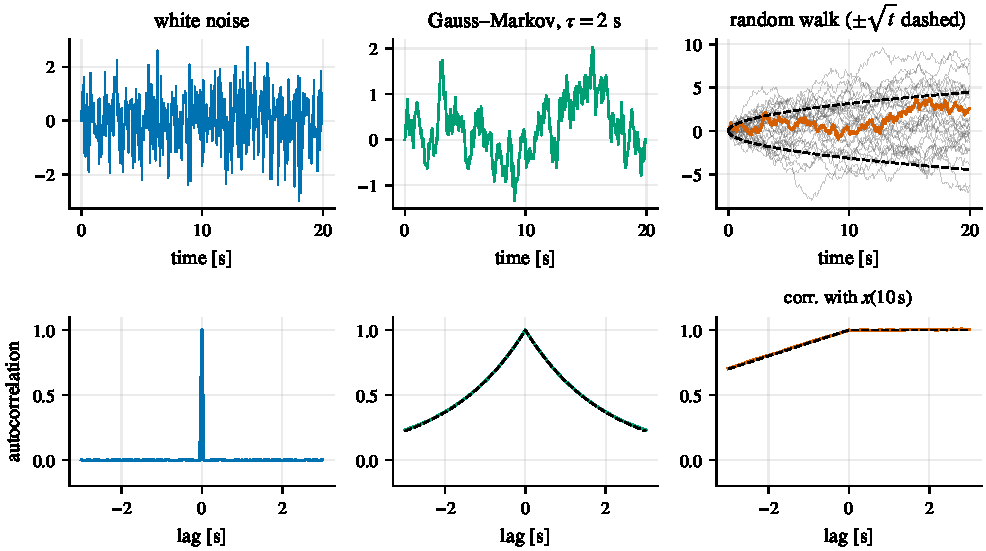
\includegraphics[width=\textwidth]{fig_processes.pdf}
  \caption{Sample paths (top) and autocorrelation functions (bottom) of white noise, a first-order Gauss--Markov sequence with correlation time
  $\tau = 2$~s, and a random walk, all driven by the same white sequence. White noise is uncorrelated with itself at any non-zero lag;
  the Gauss--Markov sequence forgets its past exponentially; the random walk never forgets and its spread grows like $\sqrt t$.}
  \label{fig:processes}
\end{figure}

\paragraph{White noise.} A \term{white sequence} has zero mean and uncorrelated values: $C(k) = \sigma^2$ for $k = 0$ and $0$ otherwise. Each
sample carries no information about the others. The measurement noise of a well-behaved sensor is approximately white.

\paragraph{Random walk.} Summing white noise gives a \term{random walk}: $x_{k+1} = x_k + w_k$, $x_0 = 0$, with $w_k$ white of variance $\sigma^2$. Then
$x_k = \sum_{j<k}w_j$ and, because variances of uncorrelated terms add,
\begin{equation}
  \Var(x_k) = k\sigma^2 .
\end{equation}
The spread grows like $\sqrt k$ without bound, and the sequence is not stationary. Its autocovariance $C(k, j) = \min(k, j)\sigma^2$ shows that
it remembers its whole past. Slowly drifting sensor biases are modeled as random walks.

\paragraph{First-order Gauss--Markov sequence.} Between the two lies $x_{k+1} = ax_k + w_k$ with $|a| < 1$. If the sequence is stationary, taking the
variance of both sides gives $V = a^2V + \sigma^2$, so
\begin{equation}
  \Var(x_k) = \frac{\sigma^2}{1 - a^2}, \qquad C(j) = \frac{\sigma^2}{1 - a^2}\,a^{|j|},
\end{equation}
the second because $x_{k+j} = a^jx_k + (\text{noise uncorrelated with } x_k)$. The sequence forgets its past exponentially, with a
\emph{correlation time} of about $1/(1 - a)$ steps. It is a bounded, slowly varying error: a useful model for biases that wander but do not
diverge, and for many environmental disturbances.

% ==============================================================================
\section{Frequency-domain description}

\subsection{Fourier analysis in brief}

Every reasonable signal is a superposition of sinusoids. The \term{Fourier transform}
\begin{equation}
  X(f) = \int_{-\infty}^{\infty}x(t)\,e^{-i2\pi ft}\,\dd t, \qquad x(t) = \int_{-\infty}^{\infty}X(f)\,e^{i2\pi ft}\,\dd f
\end{equation}
gives the complex amplitude $X(f)$ of the component at frequency $f$ (in Hz). Two facts are all we need. First, Parseval's theorem
$\int|x(t)|^2\dd t = \int|X(f)|^2\dd f$: energy can be counted in time or in frequency. Second, linear time-invariant systems (filters) act
on each frequency independently, multiplying $X(f)$ by a \emph{frequency response} $H(f)$. A low-pass filter has $|H(f)| \approx 1$ at low
frequencies and $|H(f)| \approx 0$ at high ones.

\subsection{Power spectral density}

A random signal has infinite energy (it goes on forever), but finite \emph{power}. Its \term{power spectral density} (PSD) describes how that
power is distributed over frequency.

\begin{definition}[Power spectral density]
For a wide-sense stationary process with autocovariance $C(\tau) = \E[x(t + \tau)x(t)]$ (zero mean), the (two-sided) PSD is
\begin{equation}
  S(f) = \int_{-\infty}^{\infty}C(\tau)\,e^{-i2\pi f\tau}\,\dd\tau .
\end{equation}
\end{definition}

This relation between the autocovariance and the PSD is the \emph{Wiener--Khinchin theorem}. Evaluating the inverse transform at $\tau = 0$ shows
that the variance is the total area under the PSD:
\begin{equation}
  \Var(x) = C(0) = \int_{-\infty}^\infty S(f)\,\dd f .
\end{equation}
So $S(f)\,\dd f$ is the contribution of the frequency band $[f, f + \dd f]$ to the variance, and the PSD has units of $[x]^2/\mathrm{Hz}$. Passing
the process through a filter with frequency response $H(f)$ multiplies its PSD by $|H(f)|^2$.

\begin{pitfall}[one-sided and two-sided PSDs]
Engineers often use a \emph{one-sided} PSD defined only for $f \ge 0$ and equal to twice the two-sided one, so that the variance is
$\int_0^\infty S_1(f)\,\dd f$. Datasheets rarely say which convention they use, and the two differ by a factor of $\sqrt2$ in the noise density.
These notes use the convention of the EuRoC calibration files and of most of the VIO literature: a continuous white noise $w$ with
$\E[w(t)w(s)] = \sigma^2\delta(t - s)$, i.e.\ two-sided PSD $\sigma^2$.
\end{pitfall}

% ==============================================================================
\section{Continuous-time white noise}
\label{sec:ct-noise}

\begin{definition}[Continuous-time white noise]
\index{white noise}
A zero-mean process $w(t) \in \R^n$ is white with \term{noise density} (intensity) $Q_c$ if
$\E[w(t)\,w(s)\T] = Q_c\,\delta(t - s)$, where $\delta$ is the Dirac delta. For a scalar process we write $Q_c = \sigma^2$ and call $\sigma$ the noise
density.
\end{definition}

Continuous white noise is an idealization: its PSD is flat at all frequencies, so its variance $\int S\,\dd f$ is infinite. Physical noise is
white only up to some bandwidth. What makes the idealization useful is that its \emph{integrals} are perfectly well behaved: the integral of
white noise over an interval of length $T$ is a zero-mean random variable with variance
\begin{equation}
  \Var\Big(\int_0^Tw(t)\,\dd t\Big) = \int_0^T\!\!\int_0^T\sigma^2\delta(t - s)\,\dd s\,\dd t = \sigma^2T .
\end{equation}
Since $\delta$ has units of 1/time, $\sigma$ has units of $[w]\cdot\sqrt{\mathrm s} = [w]/\sqrt{\mathrm{Hz}}$. For a gyroscope, $[w] = \mathrm{rad/s}$, so its
noise density is in $\mathrm{rad/s/\sqrt{Hz}}$, the units of \code{gyroscope\_noise\_density} in EuRoC's \code{sensor.yaml}.

\paragraph{From continuous to discrete noise.} A digital sensor reports samples every $\Dt$. If each sample is the average of the
continuous white input over its interval, which an anti-aliasing filter approximates, the sample noise has variance
\begin{equation}
  \Var\Big(\frac1\Dt\int_0^\Dt w(s)\,\dd s\Big) = \frac{\sigma^2}{\Dt}, \qquad \sigma_{\mathrm{discrete}} = \frac{\sigma}{\sqrt{\Dt}} .
  \label{eq:discrete-noise}
\end{equation}
The frequency-domain view agrees: an ideal low-pass filter that keeps the band $|f| < f_s/2$ (with $f_s = 1/\Dt$) passes a variance of
$\int_{-f_s/2}^{f_s/2}\sigma^2\,\dd f = \sigma^2f_s = \sigma^2/\Dt$. Sampling faster does not reduce the noise per unit time; it merely spreads it over
more samples, each noisier. For EuRoC's gyroscope, $\sigma_g = 1.6968\times10^{-4}~\mathrm{rad/s/\sqrt{Hz}}$ at 200~Hz gives a per-sample standard
deviation of $2.4\times10^{-3}$~rad/s.

Conversely, a random walk driven by white noise, $\dot b = w$, gains variance $\sigma^2\Dt$ over a step $\Dt$, so its exact discretization is
$b_{k+1} = b_k + \sqrt{\Dt}\,\sigma\,s_k$ with $s_k \sim \N(0, 1)$. The two conversions go in opposite directions, $\sigma/\sqrt\Dt$ for the sample noise
and $\sigma\sqrt\Dt$ for the walk; confusing them is a classic error in noise simulators.

% ==============================================================================
\section{Sampling and aliasing}

\begin{theorem}[Sampling theorem, Nyquist--Shannon]
\index{sampling theorem}
A signal containing no frequencies at or above $f_s/2$ is completely determined by its samples at rate $f_s$. The frequency $f_s/2$ is the
\term{Nyquist frequency}.
\end{theorem}

\begin{figure}[t]
  \centering
  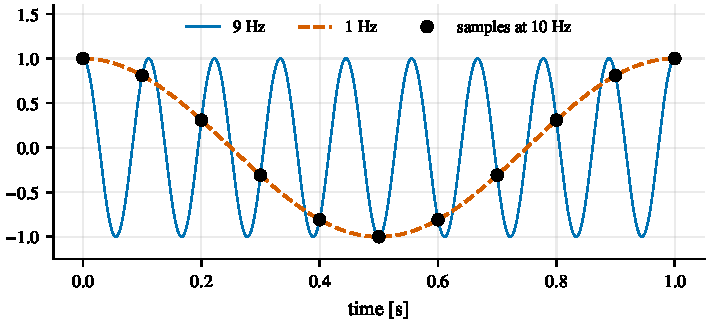
\includegraphics[width=0.9\textwidth]{fig_aliasing.pdf}
  \caption{Aliasing. A 9~Hz sinusoid sampled at 10~Hz (dots) produces exactly the same samples as a 1~Hz sinusoid (dashed). After sampling, the
  two are indistinguishable.}
  \label{fig:aliasing}
\end{figure}

A component at a frequency $f$ above the Nyquist frequency does not disappear when sampled: it masquerades as a lower frequency
$|f - kf_s|$ for the integer $k$ that brings it into $[0, f_s/2]$ (\cref{fig:aliasing}). This \term{aliasing} cannot be undone after sampling, so it
must be prevented before, by an analog or digital \emph{anti-aliasing} low-pass filter. IMUs contain such filters, but strong vibration near
or above the sampling rate (propellers at hundreds of Hz) can still alias into low frequencies and appear as bias-like errors. The same
principle governs images: a camera samples a scene spatially, and an image must be blurred before it is down-sampled, or fine textures turn
into false coarse patterns (\cref{ch:imageproc}).

% ==============================================================================
\section{Integrated noise}

\begin{proposition}[Integrated white noise]
\label{prop:integrated-noise}
Let $w$ be scalar white noise with density $\sigma$. The $m$-fold integral
$I_m(t) = \int_0^t \int_0^{t_1}\cdots\int_0^{t_{m-1}} w(t_m)\,\dd t_m \cdots \dd t_1$ has zero mean and
\begin{equation}
  \Var\big(I_m(t)\big) = \sigma^2\,\frac{t^{2m-1}}{(2m-1)\,\big((m-1)!\big)^2}.
  \label{eq:integrated-noise}
\end{equation}
For $m = 1, 2, 3, 4$ this gives $\sigma^2 t$, $\sigma^2 t^3/3$, $\sigma^2 t^5/20$ and $\sigma^2 t^7/252$.
\end{proposition}
\begin{proof}
By Cauchy's formula for repeated integration (proved by induction, exchanging the order of integration),
$I_m(t) = \int_0^t \frac{(t - s)^{m-1}}{(m-1)!}\,w(s)\,\dd s$. For a weighted integral $\int g(s)w(s)\,\dd s$ of white noise,
$\Var = \iint g(s)g(s')\,\sigma^2\delta(s - s')\,\dd s\,\dd s' = \sigma^2\int g(s)^2\,\dd s$. Here
$\int_0^t (t-s)^{2m-2}\,\dd s/((m-1)!)^2 = t^{2m-1}/((2m-1)((m-1)!)^2)$.
\end{proof}

The single integral $I_1$ is the continuous random walk, or \term{Wiener process}, whose standard deviation grows like $\sqrt t$. Integrating
accelerometer white noise twice into position gives $\sigma_a^2t^3/3$: position uncertainty grows like $t^{3/2}$. Each further integration adds
two powers of $t$ to the variance. \Cref{ch:errordyn} uses this proposition to explain how fast an inertial navigator degrades.

% ==============================================================================
\section{Linear stochastic differential equations}
\label{sec:lyapunov}

Most noise models in navigation are linear systems driven by white noise:
\begin{equation}
  \dot x(t) = F(t)\,x(t) + G(t)\,w(t), \qquad \E[w(t)w(s)\T] = Q_c\,\delta(t - s).
  \label{eq:linear-sde}
\end{equation}
Because white noise is so irregular, such equations are made rigorous by stochastic calculus. For linear systems, however, the results we
need follow from a simple limiting argument.

\begin{proposition}[Mean and covariance propagation]
\label{prop:lyapunov}
\index{Lyapunov equation}
For \eqref{eq:linear-sde}, the mean $m(t) = \E[x(t)]$ and covariance $P(t)$ evolve as
\begin{equation}
  \dot m = Fm, \qquad \dot P = FP + PF\T + GQ_cG\T,
  \label{eq:lyapunov-ode}
\end{equation}
with solution $P(t) = \Phi(t, t_0)P(t_0)\Phi(t, t_0)\T + \int_{t_0}^t\Phi(t, s)G(s)Q_cG(s)\T\Phi(t, s)\T\,\dd s$.
\end{proposition}
\begin{proof}
Over a short interval $h$, $x(t + h) = (I + Fh)x(t) + \int_t^{t+h}Gw\,\dd s + O(h^2)$, and the noise integral is zero-mean with covariance $GQ_cG\T h$ and
uncorrelated with $x(t)$. By \cref{prop:affine}, $P(t + h) = (I + Fh)P(I + Fh)\T + GQ_cG\T h + O(h^2) = P + (FP + PF\T + GQ_cG\T)h + O(h^2)$. Subtract
$P(t)$, divide by $h$ and let $h\to0$. The integral form is verified by differentiating it (\cref{prop:stm}).
\end{proof}

\Cref{eq:lyapunov-ode} is the \emph{Lyapunov differential equation}. The first two terms move and shape the existing uncertainty with the
dynamics; the last term pumps in new uncertainty from the noise. Its integral form over one time step is exactly the discrete process noise
covariance $Q_d$ of the Kalman filter (\cref{ch:linsys,ch:kf}). For a stable time-invariant system, $P$ approaches the solution of the
algebraic Lyapunov equation $0 = FP + PF\T + GQ_cG\T$.

\subsection{The continuous Gauss--Markov process}

The scalar system $\dot x = -x/\tau + w$ with noise density $\sigma$ is the continuous counterpart of the Gauss--Markov sequence. Its stationary
variance solves $0 = -2P/\tau + \sigma^2$:
\begin{equation}
  P_\infty = \frac{\sigma^2\tau}{2}, \qquad C(\Delta t) = P_\infty\,e^{-|\Delta t|/\tau}, \qquad S(f) = \frac{\sigma^2\tau^2}{1 + (2\pi f\tau)^2} .
\end{equation}
(The PSD is the white input PSD $\sigma^2$ times $|H(f)|^2$ for the system's frequency response $H(f) = 1/(i2\pi f + 1/\tau)$; integrating it over all
frequencies returns $P_\infty$.) The autocovariance decays with time constant $\tau$, and the PSD is flat up to the corner frequency $1/(2\pi\tau)$ and
falls off beyond it. Its exact discretization over $\Dt$ is $x_{k+1} = e^{-\Dt/\tau}x_k + w_k$ with $\Var(w_k) = P_\infty(1 - e^{-2\Dt/\tau})$. As
$\tau\to\infty$ it becomes a random walk; as $\tau\to0$ with the low-frequency level $\sigma^2\tau^2$ of its PSD held fixed, it becomes white noise.

% ==============================================================================
\section{Colored noise and state augmentation}

A Kalman filter assumes that its process and measurement noises are white. When a disturbance is \emph{colored} (correlated in time), the
standard remedy is to model it as the output of a linear system driven by white noise, a \emph{shaping filter}, and to add the state of that
system to the filter state. A sensor bias that drifts as a random walk is exactly this: $b$ is colored, but $\dot b = w_b$ is white-driven, so
$b$ becomes part of the state. This is why IMU biases appear in the state vector of every inertial filter (\cref{ch:imu}). Ignoring the
correlation, and treating a slowly varying error as white, makes the filter believe that errors average out when they do not, and leads to
overconfidence.

% ==============================================================================
\section{The Allan variance}
\label{sec:allan}

How are the noise densities of a sensor measured? Record it at rest for hours and compute its \term{Allan variance}, a tool developed for
characterizing atomic clocks that separates noise processes by their time scale.

\begin{definition}[Allan variance]
Split a record of rate samples $y(t)$ into consecutive clusters of duration $\tau$, and let $\bar y_k(\tau)$ be the average over cluster $k$. The
Allan variance is half the mean squared difference of consecutive cluster averages:
\begin{equation}
  \sigma_A^2(\tau) = \tfrac12\,\E\big[(\bar y_{k+1}(\tau) - \bar y_k(\tau))^2\big] .
\end{equation}
\end{definition}

In practice it is computed from the integrated signal $\theta(t) = \int_0^ty$ (for a gyroscope, the angle), since
$\bar y_{k+1} - \bar y_k = (\theta_{k+2} - 2\theta_{k+1} + \theta_k)/\tau$ with $\theta_j = \theta(j\tau)$. The \emph{overlapping} estimator averages over all
starting times rather than only disjoint clusters, which uses the data more efficiently.

\begin{proposition}[Allan variance signatures]
For white noise of density $\sigma$, $\sigma_A^2(\tau) = \sigma^2/\tau$. For a random walk $\dot b = w_b$ with density $\sigma_b$, $\sigma_A^2(\tau) = \sigma_b^2\tau/3$.
\end{proposition}
\begin{proof}
\emph{White noise.} Each cluster average is an integral of white noise divided by $\tau$, with variance $\sigma^2\tau/\tau^2 = \sigma^2/\tau$; consecutive
averages involve disjoint intervals and are uncorrelated, so their difference has variance $2\sigma^2/\tau$, and half of it is $\sigma^2/\tau$.
\emph{Random walk.} Write $b(t) = \int_0^tw_b$. The difference of two consecutive cluster averages is
$D = \frac1\tau\int_\tau^{2\tau}b\,\dd t - \frac1\tau\int_0^\tau b\,\dd t$. Substituting $b$ and exchanging the order of integration expresses $D$ as
$\frac1\tau\int_0^{2\tau}h(s)w_b(s)\,\dd s$ with $h(s) = s$ for $s \le \tau$ and $h(s) = 2\tau - s$ for $s > \tau$ (a triangular weight). Its variance is
$\frac{\sigma_b^2}{\tau^2}\big(\int_0^\tau s^2\dd s + \int_\tau^{2\tau}(2\tau - s)^2\dd s\big) = \frac{2}{3}\sigma_b^2\tau$, and half of it is $\sigma_b^2\tau/3$.
\end{proof}

On a log-log plot of the \emph{Allan deviation} $\sigma_A(\tau)$, independent noise processes therefore appear as straight lines with
characteristic slopes:
\begin{center}\small
\begin{tabular}{@{}l l l@{}}
\toprule
Process & $\sigma_A^2(\tau)$ & slope of $\sigma_A$ \\
\midrule
quantization noise & $3Q^2/\tau^2$ & $-1$ \\
white noise (density $\sigma$) & $\sigma^2/\tau$ & $-\tfrac12$ \\
bias instability ($B$) & $\approx (0.664 B)^2$ & $0$ \\
bias random walk (density $\sigma_b$) & $\sigma_b^2\tau/3$ & $+\tfrac12$ \\
rate ramp ($R$) & $R^2\tau^2/2$ & $+1$ \\
\bottomrule
\end{tabular}
\end{center}
The white-noise density is read off the $-\tfrac12$ line at $\tau = 1$~s, and the random-walk density off the $+\tfrac12$ line at $\tau = 3$~s. The
minimum of the curve marks the averaging time beyond which a stationary sensor's bias starts to wander; its height is related to the
\emph{bias instability}, a flicker-noise floor that neither white noise nor a random walk describes exactly.

\begin{figure}[t]
  \centering
  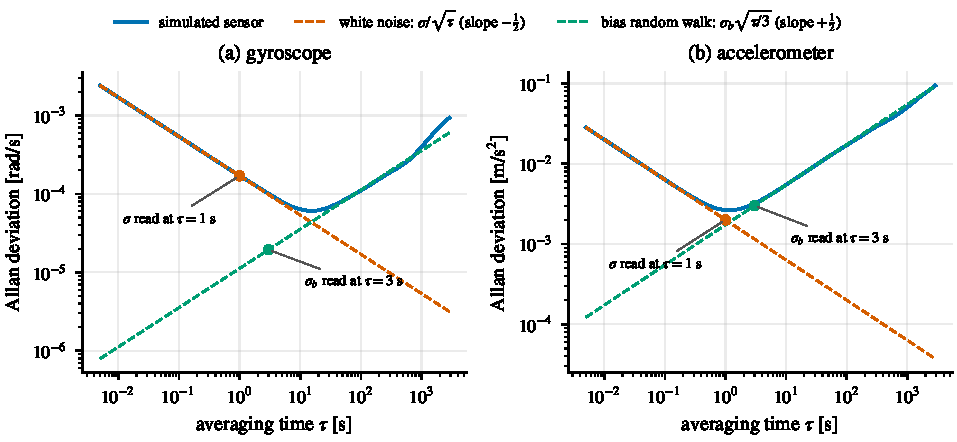
\includegraphics[width=\textwidth]{fig_allan.pdf}
  \caption{Allan deviation of a simulated 4-hour static recording with EuRoC's IMU noise parameters. The $-\tfrac12$ slope of white noise
  dominates short averaging times and the $+\tfrac12$ slope of the bias random walk dominates long ones. Reading the asymptotes at
  $\tau = 1$~s and $\tau = 3$~s recovers the densities.}
  \label{fig:allan}
\end{figure}

\Cref{fig:allan} shows the procedure on simulated data with the EuRoC parameters of \cref{ch:imu}. On real sensors, a flat bias-instability
region appears near the minimum, which the random-walk model only approximates. The IEEE standard procedure~\cite{ieee952} and El-Sheimy et
al.~\cite{elsheimy2008allan} give practical details.

\begin{takeaways}
\begin{itemize}
  \item White noise is uncorrelated in time; a random walk is its running sum, with variance growing linearly; a Gauss--Markov process
        forgets its past exponentially.
  \item The PSD distributes a process's variance over frequency; noise densities are square roots of PSDs, in units per $\sqrt{\mathrm{Hz}}$.
  \item Sampling white noise of density $\sigma$ at period $\Dt$ gives per-sample noise $\sigma/\sqrt\Dt$; a random walk gains $\sigma_b\sqrt\Dt$ per step.
  \item Frequencies above Nyquist alias; filter before you sample or down-sample.
  \item The $m$-fold integral of white noise has variance growing like $t^{2m-1}$.
  \item Covariance in a linear stochastic system obeys $\dot P = FP + PF\T + GQ_cG\T$.
  \item Colored noise is modeled with a shaping filter whose state joins the filter state: this is why biases are states.
  \item The Allan deviation separates white noise (slope $-\tfrac12$, read at 1~s) from bias random walk (slope $+\tfrac12$, read at 3~s).
\end{itemize}
\end{takeaways}

\begin{exercises}
  \item Show that the autocovariance of a random walk is $C(k, j) = \min(k, j)\,\sigma^2$.
  \item For the Gauss--Markov sequence with $a = 0.99$ and $\sigma = 1$, compute the stationary standard deviation and the lag at which the
        correlation drops below $1/e$.
  \item A 1~kHz accelerometer has white noise of $2\times10^{-3}~\mathrm{m/s^2/\sqrt{Hz}}$. What is the standard deviation of a single sample? Of the average
        of 1000 consecutive samples? Of a single sample of the same sensor read at 100~Hz?
  \item A 105~Hz vibration is sampled at 100~Hz. At what frequency does it appear?
  \item Verify \cref{prop:integrated-noise} by Monte Carlo for $m = 2$ and $m = 3$, simulating at 200~Hz for 10~s with 1000 runs.
  \item Solve the Lyapunov equation for the double integrator $\dot p = v$, $\dot v = w$ with $P(0) = 0$ and verify that $P_{pp}(t) = \sigma^2t^3/3$.
  \item Derive the stationary variance and the exact discretization of the continuous Gauss--Markov process.
  \item Simulate 2 hours of a gyro with EuRoC parameters, compute the overlapping Allan deviation, and recover $\sigma_g$ and $\sigma_{b_g}$ from the
        asymptotes. How long a recording is needed to estimate $\sigma_{b_g}$ to 10\%?
\end{exercises}

\chapter{Rotations, Quaternions and Rigid-Body Kinematics}
\label{ch:rotations}
\chaptermark{Rotations and Quaternions} % short running header

\begin{objectives}
\begin{itemize}
  \item Read and write frame-annotated transformations such as $R_{wb}$, $p_{wb}$ and $T_{bc}$ without ambiguity, and catch frame bugs
        with the adjacency rule.
  \item Understand rotations in the plane, then in space: rotation matrices, axis-angle and Rodrigues' formula.
  \item Understand Euler angles, intrinsic versus extrinsic sequences, their conversions, and why they are banned from the estimator.
  \item Derive Hamilton quaternion algebra and its rotation formula; convert between quaternions and matrices; interpolate; and
        translate formulas from the JPL convention.
  \item Derive the kinematics of rotating bodies: $\dot R = R\sx{\omega}$, $\dot q = \tfrac12 q\qprod[0,\omega]$, the transport theorem and the Coriolis
        acceleration, and quantify the effects of the Earth's rotation.
\end{itemize}
\end{objectives}

% ==============================================================================
\section{Frames and notation}

A \term{frame} is an origin together with three orthonormal, right-handed axes. Three frames appear in this project (\cref{fig:frames}).

\begin{convention}[frames, AGENTS.md C1]
\begin{itemize}
  \item $W$, the \textbf{world} frame: fixed, gravity-aligned with $z$ pointing up, the frame of the ground truth (EuRoC calls it
        \code{R}). Gravity is $g_w = [0, 0, -9.81]\T~\mathrm{m/s^2}$.
  \item $B$, the \textbf{body} frame: the IMU frame \code{imu0} (EuRoC's \code{S} in \code{imu0}).
  \item $C$, the left \textbf{camera} frame \code{cam0}: origin at the optical center, $z$ along the optical axis, $x$ to the right and $y$
        down in the image.
\end{itemize}
$R_{wb}$ (or $q_{wb}$) maps body-frame coordinates to world-frame coordinates, $v_w = R_{wb}v_b$. $p_{wb}$ is the position of the origin of $B$
expressed in $W$. $v_{wb}$ is the velocity of $B$ relative to $W$, expressed in $W$. $T_{bc} = (R_{bc}, p_{bc})$ maps camera points into the body
frame, $p_b = R_{bc}p_c + p_{bc}$; it is \code{T\_BS} from \code{cam0/sensor.yaml}. A world-to-body rotation is never used as a state.
\end{convention}

\begin{figure}[t]
\centering
\begin{tikzpicture}[scale=1.0]
  \coordinate (W) at (0,0);
  \draw[frameaxis, plotorange] (W) -- ++(1.4,0) node[right] {$x_w$};
  \draw[frameaxis, plotgreen] (W) -- ++(0.75,0.6) node[above right] {$y_w$};
  \draw[frameaxis, plotblue] (W) -- ++(0,1.4) node[above] {$z_w$};
  \node[below left] at (W) {$W$};
  \draw[->, thick, black!60] (-0.6,1.0) -- ++(0,-0.8) node[midway, left] {$g$};
  \coordinate (B) at (5.2,2.2);
  \begin{scope}[shift={(B)}, rotate=25]
    \draw[fill=primarylight, draw=primary, rounded corners=2pt] (-0.55,-0.25) rectangle (0.55,0.25);
    \draw[frameaxis, plotorange] (0,0) -- (1.3,0) node[right] {$x_b$};
    \draw[frameaxis, plotgreen] (0,0) -- (0.65,0.55) node[above right] {$y_b$};
    \draw[frameaxis, plotblue] (0,0) -- (0,1.3) node[above] {$z_b$};
    \node[below left] at (-0.2,-0.25) {$B$ (IMU)};
    \coordinate (C) at (2.0,-1.3);
    \draw[fill=white, draw=primary] ($(C)+(-0.15,0.15)$) rectangle ($(C)+(0.15,-0.15)$);
    \draw[frameaxis, plotblue] (C) -- ++(0,-0.9) node[below] {$z_c$};
    \draw[frameaxis, plotorange] (C) -- ++(0.8,0) node[right] {$x_c$};
    \draw[frameaxis, plotgreen] (C) -- ++(-0.45,-0.35) node[left] {$y_c$};
    \node[above right] at ($(C)+(0.1,0.1)$) {$C$};
    \draw[->, thick, conv] (0.3,-0.3) to[bend right=20] node[midway, below left=-1pt] {$T_{bc}$} ($(C)+(-0.2,0.05)$);
  \end{scope}
  \draw[->, thick, primary, dashed] (W) -- (B) node[midway, above left] {$p_{wb}$, $R_{wb}$};
\end{tikzpicture}
\caption{The world frame $W$ (gravity-aligned, $z$ up), the body/IMU frame $B$ moving with the vehicle, and the camera frame $C$ rigidly
attached to the body through the constant extrinsic calibration $T_{bc}$.}
\label{fig:frames}
\end{figure}

\subsection{Reading subscripts}

The naming rule \code{<quantity>\_<to><from>} makes products self-checking. $R_{wb}$ takes a vector \emph{from} $B$ \emph{to} $W$. Composition
chains frames like dominoes:
\begin{equation}
  R_{wc} = R_{wb}\,R_{bc}, \qquad v_w = R_{wb}\,R_{bc}\,v_c .
\end{equation}

\begin{keyidea}[the adjacency rule]
\index{adjacency rule}
In a valid product, adjacent subscripts match: $R_{w\underline{b}}\,R_{\underline{b}c}$. A product such as $R_{wb}R_{cb}$ has mismatched neighbors and is
a bug. The fix is a transpose, $R_{wb}R_{cb}\T = R_{wb}R_{bc}$, since $R_{bc} = R_{cb}\inv = R_{cb}\T$. Apply the rule to every line of code that
multiplies rotations or transforms points.
\end{keyidea}

\subsection{Active and passive views}

A rotation matrix can be read in two ways. In the \emph{passive} view, $R_{wb}$ re-expresses the same physical vector in another frame:
$v_w$ and $v_b$ are coordinates of one arrow (\cref{sec:orthogonal-matrices}). In the \emph{active} view, $R_{wb}$ rotates the world axes
onto the body axes: its columns are the body axes $x_b, y_b, z_b$ expressed in world coordinates. Both readings describe the same matrix:
\begin{equation}
  R_{wb} = \begin{bmatrix} x_b^{(w)} & y_b^{(w)} & z_b^{(w)} \end{bmatrix}.
\end{equation}
This gives a quick sanity check when debugging: the third column of $R_{wb}$ is the body $z$-axis in world coordinates. For a level
vehicle whose $z$-axis points up, it is $[0,0,1]\T$; its third row is the world vertical expressed in the body frame.

% ==============================================================================
\section{Rotations in the plane}

Planar rotations contain most of the ideas of this chapter in their simplest form. The rotation by $\theta$ is (\cref{ex:rot2d})
\begin{equation}
  R(\theta) = \begin{bmatrix} \cos\theta & -\sin\theta \\ \sin\theta & \cos\theta \end{bmatrix}.
\end{equation}
Rotations compose by adding angles, $R(\alpha)R(\beta) = R(\alpha + \beta)$ (multiply out and use the angle-addition formulas), so planar
rotations commute. The angle is a perfect coordinate: $R(\theta)$ is determined by $\theta$, and every planar rotation is $R(\theta)$ for a
$\theta$ that is unique up to multiples of $2\pi$. The only subtlety is wrap-around: angles must be compared modulo $2\pi$, which is why the
difference between two headings is computed as $\atantwo(\sin(\theta_2 - \theta_1), \cos(\theta_2 - \theta_1))$ rather than $\theta_2 - \theta_1$.

Identifying the plane with the complex numbers, rotation by $\theta$ is multiplication by $e^{i\theta} = \cos\theta + i\sin\theta$. Unit complex
numbers compose by multiplication, and their angles add. Quaternions (\cref{sec:quaternions}) are the three-dimensional generalization of
this idea, with one crucial difference: in three dimensions, rotations do not commute.

% ==============================================================================
\section{Rotation matrices and \texorpdfstring{$\SO$}{SO(3)}}

\begin{definition}[Special orthogonal group]
\index{special orthogonal group}
$\SO = \{ R \in \R^{3\times3} : R\T R = I,\ \det R = +1 \}$.
\end{definition}

Orthogonality ($R\T R = I$) means $R$ preserves lengths and angles; $\det R = +1$ excludes reflections, which would turn a right-handed
frame into a left-handed one (\cref{sec:orthogonal-matrices}). The set is closed under multiplication and inversion, $R\inv = R\T$, so it is
a \emph{group}. A rotation matrix has nine entries but only three degrees of freedom: orthonormality imposes six constraints (three unit
lengths, three orthogonalities). This redundancy is why $\SO$ is a curved three-dimensional surface inside the nine-dimensional space of
matrices rather than a vector space; the sum of two rotation matrices is not a rotation matrix.

The elementary rotations about the coordinate axes follow from the planar case:
\begin{equation}
  R_x(\alpha) = \begin{bmatrix} 1 & 0 & 0 \\ 0 & c_\alpha & -s_\alpha \\ 0 & s_\alpha & c_\alpha \end{bmatrix},\quad
  R_y(\alpha) = \begin{bmatrix} c_\alpha & 0 & s_\alpha \\ 0 & 1 & 0 \\ -s_\alpha & 0 & c_\alpha \end{bmatrix},\quad
  R_z(\alpha) = \begin{bmatrix} c_\alpha & -s_\alpha & 0 \\ s_\alpha & c_\alpha & 0 \\ 0 & 0 & 1 \end{bmatrix},
\end{equation}
with $c_\alpha = \cos\alpha$, $s_\alpha = \sin\alpha$. (The signs of $R_y$ look reversed but are not: in the $z$-$x$ plane, ordered cyclically
after $y$, it is the usual planar rotation.) Rotations in space do not commute: $R_x(90^\circ)R_y(90^\circ) \ne R_y(90^\circ)R_x(90^\circ)$. Try it
with a book.

\section{Axis-angle and Rodrigues' formula}

By Euler's theorem (\cref{thm:euler-axis}), every rotation is a rotation by some angle $\theta \in [0, \pi]$ about some unit axis $u$. The pair
$(u, \theta)$ is the \term{axis-angle} representation, and $\phi = \theta u \in \R^3$ is the \term{rotation vector}: its direction is the axis and its
length the angle. The rotation vector is the central object of \cref{ch:lie}.

\begin{theorem}[Rodrigues' rotation formula]
\label{thm:rodrigues}
\index{Rodrigues' formula}
The rotation by angle $\theta$ about the unit axis $u$ is
\begin{equation}
  R = I + \sin\theta\,\sx{u} + (1 - \cos\theta)\,\sx{u}^2
    = \cos\theta\, I + (1-\cos\theta)\,u u\T + \sin\theta\,\sx{u}.
  \label{eq:rodrigues}
\end{equation}
\end{theorem}
\begin{proof}[Geometric proof]
Split any vector into components parallel and perpendicular to the axis (\cref{prop:projection-line}), $v = v_\parallel + v_\perp$ with
$v_\parallel = u u\T v$. Rotation leaves $v_\parallel$ unchanged and rotates $v_\perp$ by $\theta$ within the plane spanned by $v_\perp$ and
$u \times v_\perp = u \times v$ (a vector of the same length, rotated $90^\circ$ about $u$):
\begin{equation*}
  Rv = v_\parallel + \cos\theta\, v_\perp + \sin\theta\, u \times v .
\end{equation*}
Substituting $v_\perp = v - uu\T v = -\sx{u}^2 v$ (from \eqref{eq:skew-sq} with $\|u\|=1$) and $u \times v = \sx{u}v$ gives
$Rv = (I + \sin\theta\sx{u} + (1 - \cos\theta)\sx{u}^2)v$.
\end{proof}
\begin{proof}[Algebraic proof]
The rotation about $u$ at unit angular rate satisfies $\dot R = \sx{u} R$ (\cref{sec:rot-kinematics}), so $R(\theta) = \exp(\theta\sx{u})$ by
\cref{thm:lti-solution}. With $\sx{u}^3 = -\sx{u}$ from \eqref{eq:skew-cube}, all odd powers of $\sx{u}$ are $\pm\sx{u}$ and all even powers
(except the zeroth) are $\pm\sx{u}^2$, so the exponential series regroups as
\begin{equation*}
  \exp(\theta\sx{u}) = I + \Big(\theta - \tfrac{\theta^3}{3!} + \tfrac{\theta^5}{5!} - \cdots\Big)\sx{u}
     + \Big(\tfrac{\theta^2}{2!} - \tfrac{\theta^4}{4!} + \cdots\Big)\sx{u}^2,
\end{equation*}
and the two series are $\sin\theta$ and $1 - \cos\theta$.
\end{proof}

Two consequences of \eqref{eq:rodrigues} recover $(u, \theta)$ from $R$. Taking the trace (using $\tr\sx{u} = 0$ and $\tr\sx{u}^2 = -2$) and the
skew-symmetric part,
\begin{equation}
  \tr R = 1 + 2\cos\theta, \qquad R - R\T = 2\sin\theta\,\sx{u}.
  \label{eq:trace-angle}
\end{equation}
\Cref{ch:lie} shows that \emph{how} these are combined numerically matters a great deal.

\begin{worked}[a quarter turn]
Rotate by $\theta = 90^\circ$ about $u = e_z$: $\sx{e_z} = \begin{bmatrix}0 & -1 & 0\\1 & 0 & 0\\0 & 0 & 0\end{bmatrix}$ and
$\sx{e_z}^2 = \diag(-1, -1, 0)$, so \eqref{eq:rodrigues} gives $R = \begin{bmatrix}0 & -1 & 0\\ 1 & 0 & 0\\ 0 & 0 & 1\end{bmatrix} = R_z(90^\circ)$, which
sends $e_x$ to $e_y$, as a counter-clockwise quarter turn about $z$ should. Its trace is $1 = 1 + 2\cos90^\circ$.
\end{worked}

% ==============================================================================
\section{Euler angles}

\subsection{Definition and the two readings}

\term{Euler angles} describe a rotation as three successive rotations about coordinate axes. The aerospace yaw-pitch-roll ($ZYX$)
convention writes
\begin{equation}
  R_{wb} = R_z(\psi)\,R_y(\vartheta)\,R_x(\varphi),
  \label{eq:zyx}
\end{equation}
with yaw $\psi$, pitch $\vartheta$ and roll $\varphi$. The same product can be read in two ways, which are a constant source of confusion:
\begin{itemize}
  \item \emph{Intrinsic} (rotating axes): start aligned with the world, yaw by $\psi$ about $z$, then pitch by $\vartheta$ about the \emph{new} $y$-axis,
        then roll by $\varphi$ about the \emph{newest} $x$-axis. This is how a pilot thinks.
  \item \emph{Extrinsic} (fixed axes): roll by $\varphi$ about the world $x$-axis, then pitch by $\vartheta$ about the world $y$-axis, then yaw by $\psi$ about
        the world $z$-axis.
\end{itemize}
Both readings produce the same matrix \eqref{eq:zyx}; the intrinsic sequence $z, y', x''$ equals the extrinsic sequence $x, y, z$ in reverse
order. Twelve different axis sequences are in use, and each library documents its own. Always check the convention against a known example
before trusting a conversion.

\subsection{Conversions}

Multiplying out \eqref{eq:zyx} gives the third row of $R$ as $(-\sin\vartheta,\ \cos\vartheta\sin\varphi,\ \cos\vartheta\cos\varphi)$ and the first column as
$\cos\vartheta(\cos\psi, \sin\psi, \cdot)$. Hence
\begin{equation}
  \vartheta = \atantwo\big(-R_{31},\ \sqrt{R_{11}^2 + R_{21}^2}\big), \qquad
  \varphi = \atantwo(R_{32},\ R_{33}), \qquad
  \psi = \atantwo(R_{21},\ R_{11}) .
\end{equation}
When $\cos\vartheta = 0$ ($\vartheta = \pm90^\circ$), the formulas for $\varphi$ and $\psi$ become $\atantwo(0, 0)$: only their sum or difference is determined.

\subsection{Gimbal lock}

The relation between the body angular velocity measured by a gyroscope and the rates of the Euler angles is
\begin{equation}
  \begin{bmatrix} \dot\varphi \\ \dot\vartheta \\ \dot\psi \end{bmatrix}
  = \begin{bmatrix}
      1 & \sin\varphi\tan\vartheta & \cos\varphi\tan\vartheta \\
      0 & \cos\varphi & -\sin\varphi \\
      0 & \sin\varphi/\cos\vartheta & \cos\varphi/\cos\vartheta
    \end{bmatrix} \omega_b ,
  \label{eq:euler-rates}
\end{equation}
obtained by differentiating \eqref{eq:zyx} and comparing with $\sx{\omega_b} = R\T\dot R$ (\cref{sec:rot-kinematics}). At $\vartheta = \pm90^\circ$ the
matrix blows up. Geometrically, when the nose points straight up, yaw and roll rotate about the same physical axis, so the three angles no
longer describe three independent motions. This is \term{gimbal lock}, named after mechanical gimbal platforms that physically jam in this
configuration. Near the singularity, small angular velocities produce enormous Euler-angle rates, and a filter that linearizes in Euler
angles becomes numerically meaningless.

\begin{convention}[AGENTS.md C2]
Euler angles never appear in the estimator. They may appear only in telemetry and plots.
\end{convention}

No three-parameter representation of $\SO$ is free of singularities everywhere: a topological fact (the space $\SO$ cannot be covered by a
single chart). The solution adopted by modern estimators is to store attitude in a singularity-free \emph{redundant} representation (a unit
quaternion or a rotation matrix) and to use three parameters only for \emph{small} deviations around the current estimate, where no
singularity is near. That is the content of \cref{ch:lie}.

% ==============================================================================
\section{Quaternions}
\label{sec:quaternions}

\subsection{Quaternion algebra}

\index{quaternion}
A \term{quaternion} is a four-component number $q = w + x\,i + y\,j + z\,k$, written as a scalar part and a vector part, $q = [w,\ v]$ with
$v = (x,y,z)\T$. Hamilton's multiplication rules for the three imaginary units are
\begin{equation}
  i^2 = j^2 = k^2 = ijk = -1,
\end{equation}
from which $ij = k = -ji$, $jk = i = -kj$ and $ki = j = -ik$. (For example, multiplying $ijk = -1$ on the right by $k$ gives $ij(-1) = -k$.)
Expanding the product of two quaternions term by term with these rules and collecting the scalar and vector parts gives
\begin{equation}
  p \qprod q = \begin{bmatrix} p_w q_w - p_v\T q_v \\ p_w q_v + q_w p_v + p_v \times q_v \end{bmatrix}.
  \label{eq:qprod}
\end{equation}
The products of imaginary units produce exactly the components of the cross product, which makes the product non-commutative:
$p\qprod q - q\qprod p = [0,\ 2p_v\times q_v]$. It is associative. Because it is linear in each factor, it can be written with matrices,
\begin{equation}
  p\qprod q = [p]_L\, q = [q]_R\, p, \qquad
  [p]_L = \begin{bmatrix} p_w & -p_v\T \\ p_v & p_w I + \sx{p_v} \end{bmatrix}, \quad
  [q]_R = \begin{bmatrix} q_w & -q_v\T \\ q_v & q_w I - \sx{q_v} \end{bmatrix},
\end{equation}
where quaternions are treated as 4-vectors $[q_w;\ q_v]$.

The \emph{conjugate} is $q^* = [w,\ -v]$ and the \emph{norm} is $\|q\| = \sqrt{w^2 + \|v\|^2}$. By \eqref{eq:qprod}, $q\qprod q^* = [\|q\|^2,\ 0]$, so the
inverse is $q\inv = q^*/\|q\|^2$. Conjugation reverses products, $(p\qprod q)^* = q^*\qprod p^*$, and norms multiply, $\|p\qprod q\| = \|p\|\|q\|$
(because $\|p\qprod q\|^2 = p\qprod q\qprod q^*\qprod p^* = \|q\|^2\,p\qprod p^* = \|p\|^2\|q\|^2$). Consequently the product of two \emph{unit}
quaternions is a unit quaternion: unit quaternions form a group, the three-dimensional sphere $S^3 \subset \R^4$.

\subsection{Unit quaternions represent rotations}

Identify a vector $a \in \R^3$ with the \emph{pure} quaternion $[0, a]$.

\begin{theorem}[Rotation by a unit quaternion]
\label{thm:quat-rotation}
For a unit quaternion $q = [w, v]$, the map $a \mapsto q\qprod[0, a]\qprod q^*$ sends pure quaternions to pure quaternions and acts on $a$ as the rotation
matrix
\begin{equation}
  R(q) = (w^2 - v\T v)\,I + 2\,v v\T + 2w\,\sx{v}
  = \begin{bmatrix}
    1 - 2(y^2 + z^2) & 2(xy - wz) & 2(xz + wy) \\
    2(xy + wz) & 1 - 2(x^2 + z^2) & 2(yz - wx) \\
    2(xz - wy) & 2(yz + wx) & 1 - 2(x^2 + y^2)
  \end{bmatrix}.
  \label{eq:quat-to-rot}
\end{equation}
The unit quaternion of a rotation by $\theta$ about the unit axis $u$ is
\begin{equation}
  q = \big[\cos(\theta/2),\ \sin(\theta/2)\,u\big].
  \label{eq:quat-axis-angle}
\end{equation}
\end{theorem}
\begin{proof}
By \eqref{eq:qprod}, $[0, a]\qprod q^* = [a\T v,\ wa - a\times v]$. Multiplying on the left by $q = [w, v]$:
the scalar part is $w\,a\T v - v\T(wa - a\times v) = 0$ (since $v\T(a\times v) = 0$), and the vector part is
$w(wa - a\times v) + (a\T v)v + v\times(wa - a\times v) = w^2a + 2w\,v\times a + (v\T a)v - v\times(a\times v)$. With the BAC--CAB rule,
$v\times(a\times v) = a\,(v\T v) - v\,(v\T a)$, so the vector part is $(w^2 - v\T v)a + 2(v\T a)v + 2w\,v\times a$, which is \eqref{eq:quat-to-rot}. This
matrix is orthogonal with determinant one (it preserves norms, because quaternion norms multiply, and depends continuously on $q$, equal to
$I$ at $q = [1, 0]$). For \eqref{eq:quat-axis-angle}, substitute $w = \cos\frac\theta2$, $v = \sin\frac\theta2 u$ and use the double-angle identities
$w^2 - v\T v = \cos\theta$, $2\sin^2\frac\theta2 = 1 - \cos\theta$ and $2\sin\frac\theta2\cos\frac\theta2 = \sin\theta$; the result is the second form of
Rodrigues' formula \eqref{eq:rodrigues}.
\end{proof}

The \emph{half} angle in \eqref{eq:quat-axis-angle} is the most common source of factor-of-two bugs. It arises because $q$ appears twice in the
sandwich product $q \qprod [0,a] \qprod q^*$, each occurrence contributing half of the rotation.

\begin{keyidea}[double cover]
\index{double cover}
$q$ and $-q$ give the same $R(q)$, since \eqref{eq:quat-to-rot} is quadratic in $q$. Every rotation has exactly two unit quaternions, at opposite
points of the sphere $S^3$. They correspond to rotating by $\theta$ about $u$, or by $2\pi - \theta$ about $-u$. Code that compares, averages,
interpolates or takes logarithms of quaternions must account for this. The project canonicalizes to $w \ge 0$ before taking $\Log_q$
(AGENTS.md C2).
\end{keyidea}

\subsection{Composition}

Because $(p\qprod q)\qprod[0, a]\qprod(p\qprod q)^* = p\qprod\big(q\qprod[0, a]\qprod q^*\big)\qprod p^*$, the Hamilton product composes rotations in the same order
as matrix multiplication:
\begin{equation}
  R(p \qprod q) = R(p)\,R(q), \qquad q_{wc} = q_{wb}\qprod q_{bc} \ \leftrightarrow\ R_{wc} = R_{wb}R_{bc}.
\end{equation}
The adjacency rule therefore applies to quaternions unchanged. Composing quaternions costs 16 multiplications and 12 additions, against 27 and
18 for matrices, and renormalizing a quaternion is trivial compared with re-orthogonalizing a matrix. These are the practical reasons to
store attitude as a quaternion.

\begin{worked}[composing two quarter turns]
The quarter turn about $z$ is $q_z = [\cos45^\circ,\ \sin45^\circ e_z] = \frac{1}{\sqrt2}[1, (0,0,1)]$, and about $x$ it is
$q_x = \frac{1}{\sqrt2}[1, (1,0,0)]$. By \eqref{eq:qprod}, $q_z\qprod q_x = \tfrac12\big[1,\ (1, 0, 1) + e_z\times e_x\big] = \tfrac12[1, (1, 1, 1)]$: a rotation by
$2\arccos\frac12 = 120^\circ$ about $(1,1,1)/\sqrt3$. (Check: it cycles the axes, $x\to y\to z\to x$.) In the other order,
$q_x\qprod q_z = \tfrac12[1, (1, -1, 1)]$, a different rotation.
\end{worked}

\subsection{Converting a rotation matrix to a quaternion}

Inverting \eqref{eq:quat-to-rot} naively via $w = \tfrac12\sqrt{1 + \tr R}$ and $v = (R - R\T)\veeop/(4w)$ divides by a number that vanishes for
$180^\circ$ rotations. \emph{Shepperd's method} avoids this. From \eqref{eq:quat-to-rot}, the four quantities
$4w^2 = 1 + \tr R$, $4x^2 = 1 + R_{11} - R_{22} - R_{33}$, $4y^2 = 1 - R_{11} + R_{22} - R_{33}$ and $4z^2 = 1 - R_{11} - R_{22} + R_{33}$ can all be computed
from the diagonal. Choose the largest (at least $1/4$, since $w^2 + x^2 + y^2 + z^2 = 1$), take its square root, and compute the other three components
from the off-diagonal sums and differences, for example $4wx = R_{32} - R_{23}$, $4xy = R_{21} + R_{12}$, $4xz = R_{13} + R_{31}$, dividing only by the large
component. Eigen implements this method.

\subsection{The Hamilton and JPL conventions}

Unfortunately, two incompatible quaternion conventions are in wide use. Much of the classic VIO literature, including the original MSCKF
paper~\cite{mourikis2007msckf} and the indirect Kalman filter report of Trawny and Roumeliotis~\cite{trawny2005indirect}, uses the
\emph{JPL} convention. Formulas cannot be copied between the two without translation~\cite{sommer2018flipped}.

\begin{table}[h]
\centering\small
\begin{tabularx}{\textwidth}{@{}l X X@{}}
\toprule
 & \textbf{Hamilton (this project)} & \textbf{JPL} \\
\midrule
Multiplication rule & $ij = k$ ($ijk = -1$) & $ij = -k$ ($ijk = +1$) \\
Component order & usually $[w, x, y, z]$ & usually $[x, y, z, w]$ \\
Typical meaning & body-to-world (active), $q_{wb}$ & world-to-body (passive), ${}^{B}_{W}\bar q$ \\
Composition & $q_{wc} = q_{wb}\qprod q_{bc}$ & ${}^{C}_{W}\bar q = {}^{C}_{B}\bar q\otimes{}^{B}_{W}\bar q$ \\
Rotation matrix & $R(q) = (w^2 - v\T v)I + 2vv\T + 2w\sx{v}$ & $C(\bar q) = (2q_4^2 - 1)I - 2q_4\sx{q} + 2qq\T$ \\
Used by & Eigen, ROS, Sol\`a~\cite{sola2017quaternion}, Ceres, Sophus & MSCKF papers, Trawny~\cite{trawny2005indirect}, NASA \\
\bottomrule
\end{tabularx}
\caption{Hamilton versus JPL quaternions. The JPL product of two quaternions equals the Hamilton product of the same numbers in reverse order.}
\label{tab:hamilton-jpl}
\end{table}

A useful fact for reading the JPL literature: the JPL quaternion ${}^B_W\bar q$ of the world-to-body rotation has \emph{the same four numbers} as the
Hamilton quaternion $q_{wb}$ of the body-to-world rotation, merely stored in the order $[x, y, z, w]$. (Substitute into the two rotation formulas of
\cref{tab:hamilton-jpl}: $C(\bar q) = R(q)\T$.) What changes is the meaning of products and of perturbations: a JPL error quaternion
$\delta\bar q$ in ${}^B_W\bar q = \delta\bar q\otimes{}^B_W\hat{\bar q}$ is a perturbation in the body frame, but written on the left, and its Jacobians differ in sign
and order from ours. Translate a JPL derivation by re-deriving it, not by pattern-matching symbols.

\begin{convention}[quaternions, AGENTS.md C2]
Hamilton quaternions, \code{Eigen::Quaterniond}, always of unit norm, normalized after every multiplicative update. Never substitute JPL
formulas, even when a paper you are reading uses them. Translate them first.
\end{convention}

\subsection{Quaternions in code and data}

\begin{pitfall}[coefficient order]
Three orderings meet at the project's input boundary:
\begin{itemize}
  \item \code{Eigen::Quaterniond(w, x, y, z)}: the constructor takes $w$ \emph{first};
  \item \code{q.coeffs()}: Eigen's storage is $[x, y, z, w]$, with $w$ \emph{last};
  \item EuRoC CSV files store \code{qw, qx, qy, qz}, with $w$ first.
\end{itemize}
Mapping a raw EuRoC row with \code{Eigen::Map<Quaterniond>} interprets it as $[x,y,z,w]$ and silently produces a different, valid-looking
rotation. Always construct explicitly, \code{Eigen::Quaterniond(row[0], row[1], row[2], row[3])}, and cover the parser with a fixture test.
\end{pitfall}

Other Eigen facts worth knowing: \code{q * v} for a \code{Vector3d} applies $R(q)$ to $v$; \code{q1 * q2} is the Hamilton product;
\code{q.conjugate()} is the inverse of a unit quaternion; \code{q.normalize()} works in place while \code{q.normalized()} returns a copy; and
\code{q.toRotationMatrix()} evaluates \eqref{eq:quat-to-rot}.

\paragraph{Normalization.} Each multiplicative update of a quaternion rounds its four components, so $\|q\|$ performs a slow random walk away
from $1$. A non-unit quaternion inserted into \eqref{eq:quat-to-rot} produces a matrix that scales vectors by $\|q\|^2$ as well as rotating them.
Dividing by the norm after every update costs a few flops and removes the problem. Milestone 4 checks that $|\|q\| - 1| < 10^{-12}$ after
$10^6$ updates.

\subsection{Distance and interpolation}

The angle of the relative rotation between two attitudes $q_1$ and $q_2$ is
\begin{equation}
  \theta_{12} = 2\arccos\big|q_1\T q_2\big| = \big\|\Log_q(q_1\inv\qprod q_2)\big\|,
\end{equation}
where $q_1\T q_2$ is the four-dimensional dot product (the scalar part of $q_1^*\qprod q_2$) and the absolute value accounts for the double cover.
(For small angles prefer the $\Log_q$ form, which avoids $\arccos$ near 1; \cref{ch:lie}.)

\begin{figure}[t]
  \centering
  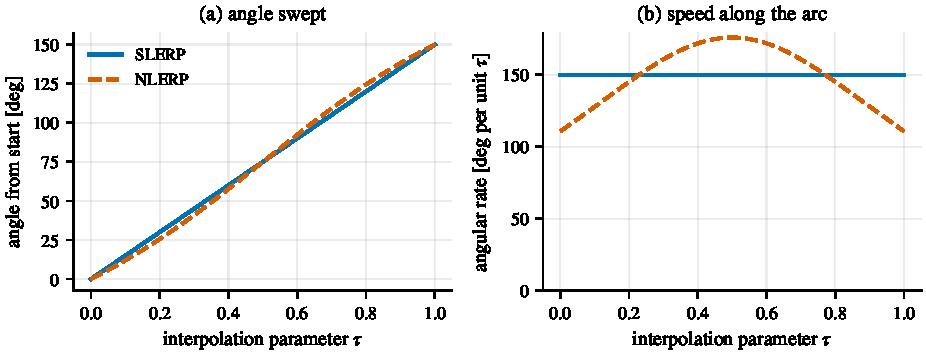
\includegraphics[width=0.84\textwidth]{fig_slerp.pdf}
  \caption{Interpolating between two attitudes $150^\circ$ apart. SLERP sweeps the angle uniformly in the interpolation parameter; normalized linear
  interpolation (NLERP) follows the same path but at a non-uniform speed, fastest in the middle.}
  \label{fig:slerp}
\end{figure}

Ground truth and IMU data rarely share timestamps with images, so attitudes must be interpolated. The correct interpolation follows the
shortest great arc at constant angular velocity: \term{spherical linear interpolation} (SLERP),
\begin{equation}
  q(\tau) = q_0 \qprod \Exp_q\!\big(\tau\,\Log_q(q_0\inv\qprod q_1)\big)
          = \frac{\sin((1 - \tau)\Omega)}{\sin\Omega}\,q_0 + \frac{\sin(\tau\Omega)}{\sin\Omega}\,q_1,
  \qquad \tau\in[0,1],
\end{equation}
with $\cos\Omega = q_0\T q_1$ after flipping the sign of $q_1$ if needed so that $q_0\T q_1 \ge 0$. The first form (using the exponential and
logarithm of \cref{ch:lie}) shows that the relative rotation is applied with a uniformly growing angle; the second is the formula for
interpolating along a great circle of the sphere. Component-wise linear interpolation followed by normalization (NLERP) follows the same
path at a non-uniform speed (\cref{fig:slerp}); it is acceptable only for small angles.

% ==============================================================================
\section{Rigid-body transformations}

A rigid transformation combines a rotation and a translation. Point coordinates transform as
\begin{equation}
  p_w = R_{wb}\,p_b + p_{wb}
  \quad\Longleftrightarrow\quad
  \begin{bmatrix} p_w \\ 1 \end{bmatrix} = \underbrace{\begin{bmatrix} R_{wb} & p_{wb} \\ 0 & 1 \end{bmatrix}}_{T_{wb}}
  \begin{bmatrix} p_b \\ 1 \end{bmatrix}.
\end{equation}
Appending a 1 to the point (\emph{homogeneous coordinates}, developed in \cref{ch:camera}) turns the affine map into a single matrix product.
The $4\times4$ matrices of this form make up the group $\SE$ of rigid motions. Composition and inversion follow from block multiplication:
\begin{equation}
  T_{wc} = T_{wb}T_{bc} = \begin{bmatrix} R_{wb}R_{bc} & R_{wb}p_{bc} + p_{wb} \\ 0 & 1\end{bmatrix},
  \qquad
  T_{wb}\inv = T_{bw} = \begin{bmatrix} R_{wb}\T & -R_{wb}\T p_{wb} \\ 0 & 1 \end{bmatrix}.
  \label{eq:se3-compose}
\end{equation}
The camera pose in the world therefore is $R_{wc} = R_{wb}R_{bc}$ and $p_{wc} = p_{wb} + R_{wb}p_{bc}$, and a world point $p_f$ has camera coordinates
\begin{equation}
  p_c = R_{bc}\T\big(R_{wb}\T(p_f - p_{wb}) - p_{bc}\big),
  \label{eq:world-to-camera}
\end{equation}
which is the first half of the camera measurement model (AGENTS.md C6).

\begin{pitfall}[points versus directions]
Translations apply to points, not to free vectors. A velocity, a gravity vector or a bearing direction transforms with the rotation only,
$v_w = R_{wb}v_b$. In homogeneous coordinates directions carry a $0$ in the fourth component, which drops the translation automatically.
\end{pitfall}

% ==============================================================================
\section{Rotational kinematics}
\label{sec:rot-kinematics}

\subsection{Angular velocity}

Let $R(t) = R_{wb}(t)$ describe a rotating body. Differentiating $R\T R = I$ gives $\dot R\T R + R\T\dot R = 0$, so $R\T\dot R$ is skew-symmetric and
equals $\sx{\omega_b}$ for a unique vector $\omega_b$:
\begin{equation}
  \dot R_{wb} = R_{wb}\,\sx{\omega_b} = \sx{\omega_w}\,R_{wb}, \qquad \omega_w = R_{wb}\,\omega_b ,
  \label{eq:rdot}
\end{equation}
where the second form uses \eqref{eq:skew-rot}. Why is $\omega$ an angular velocity? A point fixed in the body, with constant body coordinates $r_b$,
has world coordinates $r_w = R_{wb}r_b$ and velocity $\dot r_w = \dot R_{wb}r_b = \sx{\omega_w}R_{wb}r_b = \omega_w\times r_w$: every point moves as if the body
were spinning about the axis $\omega_w$ through the origin with angular speed $\|\omega\|$. $\omega_b$ is this angular velocity of $B$ relative to $W$,
expressed in $B$, and it is exactly what a strapdown gyroscope measures (up to bias and noise). The two forms of \eqref{eq:rdot} are the
kinematic origin of the two perturbation conventions of \cref{ch:lie}: a body-frame quantity multiplies on the right, a world-frame quantity on
the left.

\begin{proposition}[Constant body rate]
\label{prop:const-rate}
If $\omega_b$ is constant on $[t_0, t_0 + \Dt]$, then $R(t_0 + \Dt) = R(t_0)\exp(\Dt\sx{\omega_b})$.
\end{proposition}
\begin{proof}
$R(t) = R(t_0)\exp((t - t_0)\sx{\omega_b})$ satisfies \eqref{eq:rdot} by \cref{prop:matexp}, and the solution is unique (\cref{thm:lti-solution}).
\end{proof}

This exact solution is the basis of the multiplicative attitude update used in every integration scheme of \cref{ch:strapdown}. When the
rate varies, the update is still applied step by step with the rate held constant over each short step (\cref{sec:lie-euler}). Note that the
solution is \emph{not} $R(t_0) + \Dt\, R(t_0)\sx{\omega_b}$, which would leave $\SO$.

\subsection{Quaternion kinematics}

The quaternion counterpart of \eqref{eq:rdot} is
\begin{equation}
  \dot q_{wb} = \tfrac12\, q_{wb} \qprod [0,\ \omega_b] = \tfrac12\,\Omega(\omega_b)\,q_{wb},
  \qquad \Omega(\omega) = [\,[0, \omega]\,]_R = \begin{bmatrix} 0 & -\omega\T \\ \omega & -\sx{\omega}\end{bmatrix},
  \label{eq:qdot}
\end{equation}
with constant-rate solution $q(t_0 + \Dt) = q(t_0)\qprod\big[\cos\tfrac{\|\omega\|\Dt}{2},\ \sin\tfrac{\|\omega\|\Dt}{2}\,\tfrac{\omega}{\|\omega\|}\big]$. To derive
\eqref{eq:qdot}, compose $q(t + \dd t) = q(t) \qprod \dd q$, where $\dd q$ is the small body-frame rotation by $\omega_b\,\dd t$. By
\eqref{eq:quat-axis-angle}, $\dd q = [1,\ \tfrac12\omega_b\,\dd t] + O(\dd t^2)$, so $q(t + \dd t) - q(t) = q\qprod[0, \tfrac12\omega_b]\,\dd t$. The factor $\tfrac12$ is
the half angle again.

\subsection{Derivatives in a rotating frame}

Differentiating $v_w = R_{wb}v_b$ with \eqref{eq:rdot} gives the \term{transport theorem}
\begin{equation}
  \dot v_w = R_{wb}\big(\dot v_b + \omega_b \times v_b\big):
  \label{eq:transport}
\end{equation}
the rate of change seen from the fixed frame equals the rate seen in the rotating frame plus the change due to the rotation of the frame itself.
Applying it twice to the position $r$ of a particle relative to a frame rotating with angular velocity $\Omega$ (constant) gives the acceleration
in the fixed (inertial) frame, expressed in rotating coordinates:
\begin{equation}
  a_{\mathrm{inertial}} = \ddot r + 2\,\Omega\times\dot r + \Omega\times(\Omega\times r),
  \label{eq:coriolis}
\end{equation}
where $\ddot r$ and $\dot r$ are the acceleration and velocity seen in the rotating frame. The extra terms are the \term{Coriolis acceleration}
$2\Omega\times\dot r$ and the \term{centripetal acceleration} $\Omega\times(\Omega\times r)$. This formula is the working principle of the vibratory MEMS gyroscope
(\cref{ch:imu}), and it tells us what we neglect by treating the world frame as inertial.

\subsection{The Earth is not an inertial frame}

The world frame $W$ is fixed to the Earth, which rotates at $\Omega_e = 7.292\times10^{-5}$~rad/s. Three effects follow; their sizes justify the
project's simplifications.
\begin{itemize}
  \item \emph{Gyroscopes sense the Earth rate.} $7.3\times10^{-5}$~rad/s is comparable to the bias instability of the EuRoC ADIS16448 and far below its
        noise over short horizons. The project neglects it; its constant body-frame component (while the attitude changes little) is absorbed
        by the gyro bias estimate. High-grade systems model it explicitly and can even find north from it (gyrocompassing).
  \item \emph{Centripetal acceleration.} The term $\Omega_e\times(\Omega_e\times r)$ reaches $0.034~\mathrm{m/s^2}$ at the equator. It is absorbed into the
        local gravity vector: \emph{gravity}, as measured by a plumb line, is gravitation plus this centrifugal term. Its magnitude varies from
        $9.780~\mathrm{m/s^2}$ at the equator to $9.832~\mathrm{m/s^2}$ at the poles; the project uses a constant $9.81$ (AGENTS.md C5), accurate to about
        $10^{-3}$ relative in Zurich, where EuRoC was recorded.
  \item \emph{Coriolis acceleration.} $2\Omega_e\times v$ is about $1.5\times10^{-4}~\mathrm{m/s^2}$ at 1~m/s: below accelerometer noise and bias for a small
        drone, and neglected.
\end{itemize}
Over the minutes and hundreds of meters of a EuRoC sequence, the world frame may therefore be treated as inertial and flat, with constant
gravity.

\begin{takeaways}
\begin{itemize}
  \item $R_{wb}$ maps body coordinates to world coordinates; its columns are the body axes in the world. Adjacent subscripts must match.
  \item Every rotation is an axis-angle rotation, $R = I + \sin\theta\sx{u} + (1-\cos\theta)\sx{u}^2$; $\tr R = 1 + 2\cos\theta$.
  \item Euler angles have intrinsic and extrinsic readings and a singularity at $\pm90^\circ$ pitch; they stay out of the estimator.
  \item Hamilton unit quaternions compose like matrices; $q$ and $-q$ are the same rotation; the quaternion of a rotation by $\theta$ uses $\theta/2$.
  \item Eigen's constructor is $w$-first, its storage $w$-last, EuRoC is $w$-first. JPL formulas must be re-derived, not copied.
  \item $\dot R_{wb} = R_{wb}\sx{\omega_b}$; with constant $\omega_b$ the update $R \leftarrow R\exp(\Dt\sx{\omega_b})$ is exact.
  \item Derivatives in rotating frames pick up $\omega\times$ terms; for a small drone over minutes, the Earth's rotation is negligible.
\end{itemize}
\end{takeaways}

\begin{exercises}
  \item Show that the columns of any $R \in \SO$ are orthonormal and that $\det R = +1$ implies the third column is the cross product of the first two.
  \item Verify $R_x(90^\circ)R_y(90^\circ) \neq R_y(90^\circ)R_x(90^\circ)$ by computing both products, and describe each rotation physically.
  \item Derive \eqref{eq:euler-rates} from \eqref{eq:zyx} and $\sx{\omega_b} = R\T\dot R$.
  \item Convert the rotation of the worked example ($120^\circ$ about $(1,1,1)/\sqrt3$) to ZYX Euler angles.
  \item Prove that $[p]_L[q]_R = [q]_R[p]_L$. What does this say about associativity of the quaternion product?
  \item Show that $R(-q) = R(q)$ and compute the quaternion of a $270^\circ$ rotation about $z$ in its canonical form ($w \ge 0$). What rotation angle and
        axis does the canonical form describe?
  \item Implement Shepperd's method and test it on rotations by $0^\circ$, $90^\circ$, $179.9999^\circ$ and $180^\circ$.
  \item Write a function that converts a EuRoC ground-truth row into $p_{wb}$, $q_{wb}$, $v_{wb}$, $b_g$ and $b_a$. Design a fixture row whose values would
        expose a swapped $w/z$ and swapped biases.
  \item Given $T_{bc}$ from \code{cam0/sensor.yaml} (\cref{app:euroc}), compute the camera's optical axis in body coordinates.
  \item Show that if $\omega_b$ varies in time, $R(t) = R(0)\exp\big(\int_0^t\sx{\omega_b}\,\dd s\big)$ is in general \emph{wrong}. Construct a counterexample with
        piecewise-constant rates.
  \item Derive \eqref{eq:coriolis} by applying \eqref{eq:transport} twice.
\end{exercises}
% Solutions to the exercises of Chapter 7.
\begin{solutions}
  \item Write $R = [r_1\ r_2\ r_3]$. The entry $(i, j)$ of $R\T R = I$ is $r_i\T r_j = \delta_{ij}$: the columns are orthonormal. The unit vectors orthogonal
        to both $r_1$ and $r_2$ are exactly $\pm r_1\times r_2$ (a unit vector, by Lagrange's identity), so $r_3 = \pm r_1\times r_2$. The determinant is the
        triple product $\det R = r_3\T(r_1\times r_2) = \pm\|r_1\times r_2\|^2 = \pm1$, so $\det R = +1$ selects $r_3 = r_1\times r_2$: the body axes form a
        right-handed frame.

  \item From the elementary matrices,
        \[
          R_x(90^\circ)R_y(90^\circ) = \begin{bmatrix}0 & 0 & 1\\ 1 & 0 & 0\\ 0 & 1 & 0\end{bmatrix}, \qquad
          R_y(90^\circ)R_x(90^\circ) = \begin{bmatrix}0 & 1 & 0\\ 0 & 0 & -1\\ -1 & 0 & 0\end{bmatrix}.
        \]
        The first sends $e_x \to e_y$, $e_y \to e_z$, $e_z \to e_x$ (its columns): it cycles the axes, a $120^\circ$ rotation about $(1,1,1)/\sqrt3$. The
        second has trace 0 (angle $120^\circ$) and $(R - R\T)\veeop = (1, 1, -1)$, so it is a $120^\circ$ rotation about $(1, 1, -1)/\sqrt3$. Physically, read
        as intrinsic sequences: the first turns a book $90^\circ$ about its $x$-axis and then $90^\circ$ about its new $y$-axis; the second does the two
        quarter turns in the other order and leaves the book in a different orientation.

  \item Write $R = R_zR_yR_x$ with $\dot R_z = \dot\psi R_z\sx{e_z}$, $\dot R_y = \dot\vartheta R_y\sx{e_y}$, $\dot R_x = \dot\varphi R_x\sx{e_x}$. Then
        \[
          R\T\dot R = \dot\psi\,R_x\T R_y\T\sx{e_z}R_yR_x + \dot\vartheta\,R_x\T\sx{e_y}R_x + \dot\varphi\,\sx{e_x}
          = \big[\dot\psi\,R_x\T R_y\T e_z + \dot\vartheta\,R_x\T e_y + \dot\varphi\,e_x\big]_\times
        \]
        by \eqref{eq:skew-rot}. With $R_y\T e_z = (-s_\vartheta, 0, c_\vartheta)$, $R_x\T(-s_\vartheta, 0, c_\vartheta) = (-s_\vartheta, s_\varphi c_\vartheta, c_\varphi c_\vartheta)$ and
        $R_x\T e_y = (0, c_\varphi, -s_\varphi)$,
        \[
          \omega_b = \begin{bmatrix} 1 & 0 & -s_\vartheta \\ 0 & c_\varphi & s_\varphi c_\vartheta \\ 0 & -s_\varphi & c_\varphi c_\vartheta \end{bmatrix}
                     \begin{bmatrix}\dot\varphi\\ \dot\vartheta\\ \dot\psi\end{bmatrix}.
        \]
        The matrix has determinant $c_\vartheta$. Solving the last two rows gives $\dot\vartheta = c_\varphi\omega_y - s_\varphi\omega_z$ and
        $\dot\psi = (s_\varphi\omega_y + c_\varphi\omega_z)/c_\vartheta$, and the first row gives $\dot\varphi = \omega_x + s_\vartheta\dot\psi$, which is \eqref{eq:euler-rates}.
        The determinant $c_\vartheta$ vanishes at $\vartheta = \pm90^\circ$: gimbal lock.

  \item The rotation is the axis-cycling matrix of Exercise 7.2, $R = \begin{bmatrix}0 & 0 & 1\\ 1 & 0 & 0\\ 0 & 1 & 0\end{bmatrix}$. With the conversion formulas,
        $\vartheta = \atantwo(-R_{31}, \sqrt{R_{11}^2 + R_{21}^2}) = \atantwo(0, 1) = 0$, $\varphi = \atantwo(R_{32}, R_{33}) = \atantwo(1, 0) = 90^\circ$ and
        $\psi = \atantwo(R_{21}, R_{11}) = \atantwo(1, 0) = 90^\circ$: yaw $90^\circ$, pitch $0$, roll $90^\circ$. Check: $R_z(90^\circ)R_x(90^\circ)$ reproduces $R$, as the worked
        example $q_z\qprod q_x$ already showed.

  \item Apply both sides to an arbitrary quaternion $r$. By definition $[q]_Rr = r\qprod q$ and $[p]_Lr = p\qprod r$, so
        \[
          [p]_L[q]_R\,r = p\qprod(r\qprod q), \qquad [q]_R[p]_L\,r = (p\qprod r)\qprod q .
        \]
        The two agree for every $r$ exactly because the Hamilton product is associative, so the matrices are equal. (Multiplying out the blocks and
        using $\sx{a}\sx{b} = ba\T - (a\T b)I$ confirms it directly.) Conversely, the identity $[p]_L[q]_R = [q]_R[p]_L$ for all $p, q$ \emph{is} the
        statement of associativity: multiplying on the left and on the right are commuting operations.

  \item $R(q)$ in \eqref{eq:quat-to-rot} is a homogeneous quadratic in the components of $q$, so $R(-q) = (-1)^2R(q) = R(q)$. A $270^\circ$ rotation about
        $z$ has
        \[
          q = \big[\cos135^\circ,\ \sin135^\circ e_z\big] = \big[-\tfrac{\sqrt2}{2},\ (0, 0, \tfrac{\sqrt2}{2})\big].
        \]
        Its scalar part is negative, so the canonical form is $-q = [\tfrac{\sqrt2}{2},\ (0, 0, -\tfrac{\sqrt2}{2})]$. It describes a rotation by
        $2\arccos(\tfrac{\sqrt2}2) = 90^\circ$ about $-e_z$: the same rotation as $270^\circ$ about $+e_z$, reached the short way round. Canonicalization
        always yields an angle in $[0, \pi]$.

  \item A direct implementation picks the largest of the four squared components, computed from the diagonal:
\begin{lstlisting}[style=py]
def shepperd(R):
    t = np.trace(R)
    c = [1 + t, 1 + R[0,0] - R[1,1] - R[2,2], 1 - R[0,0] + R[1,1] - R[2,2], 1 - R[0,0] - R[1,1] + R[2,2]]
    i = int(np.argmax(c)); s = 2 * np.sqrt(c[i])          # s = 4 * (largest component)
    a, b, d = R[2,1] - R[1,2], R[0,2] - R[2,0], R[1,0] - R[0,1]   # 4wx, 4wy, 4wz
    e, f, g = R[0,1] + R[1,0], R[0,2] + R[2,0], R[1,2] + R[2,1]   # 4xy, 4xz, 4yz
    q = [[s/4, a/s, b/s, d/s], [a/s, s/4, e/s, f/s], [b/s, e/s, s/4, g/s], [d/s, f/s, g/s, s/4]][i]
    return np.array(q) if q[0] >= 0 else -np.array(q)
\end{lstlisting}
        Testing against the quaternion used to build each matrix (axis $(1, -2, 0.5)/\|\cdot\|$) gives errors of $0$, $3\times10^{-16}$, $2\times10^{-18}$ and
        $10^{-16}$ at $0^\circ$, $90^\circ$, $179.9999^\circ$ and $180^\circ$. The naive formula $w = \tfrac12\sqrt{1 + \tr R}$, $v = (R - R\T)\veeop/4w$ is exact at the first two,
        wrong by $9\times10^{-6}$ at $179.9999^\circ$ (it divides by $w \approx 9\times10^{-7}$, computed from the difference $1 + \tr R \approx 3\times10^{-12}$), and
        undefined at $180^\circ$.

  \item The ground-truth row is \code{timestamp, p\_x, p\_y, p\_z, q\_w, q\_x, q\_y, q\_z, v\_x, v\_y, v\_z, bw\_x, bw\_y, bw\_z, ba\_x, ba\_y, ba\_z} (AGENTS.md C7).
        In C++ the parser constructs each piece explicitly:
\begin{lstlisting}
p_wb = Eigen::Vector3d(r[1], r[2], r[3]);
q_wb = Eigen::Quaterniond(r[4], r[5], r[6], r[7]).normalized();  // w first
v_wb = Eigen::Vector3d(r[8], r[9], r[10]);
b_g  = Eigen::Vector3d(r[11], r[12], r[13]);   // gyro bias comes first
b_a  = Eigen::Vector3d(r[14], r[15], r[16]);
\end{lstlisting}
        A good fixture row makes every plausible mistake produce a detectably different result: all quaternion components distinct and of
        different signs, e.g.\ $q = (w, x, y, z) = (0.8, 0.2, -0.4, 0.4)$ (unit norm), so that reading it as $[x, y, z, w]$ gives a different rotation;
        biases of different magnitudes and signs, e.g.\ $b_g = (0.01, 0.02, 0.03)$ and $b_a = (-0.1, -0.2, -0.3)$, so that swapping them is visible;
        and position and velocity that differ in every component. The test asserts each field and also checks that $R(q)\,e_x$ equals the column
        computed by hand, which catches a wrong constructor order even when the norm is unchanged. A row with the identity quaternion, or with
        equal biases, would let all these bugs pass.

  \item The optical axis is the camera's $z$-axis; in body coordinates it is $R_{bc}e_z$, the third column of the rotation block of $T_{bc}$. With the
        values of \cref{app:euroc} it is $(0.0041, 0.0257, 0.9997)$: the camera looks along the body $+z$-axis, tilted by $\arccos(0.9997) = 1.5^\circ$. The
        other columns show the camera $x$-axis along body $+y$ and the camera $y$-axis along body $-x$; since the EuRoC IMU's $x$-axis points up at
        rest, the image $y$-axis (rows, increasing downwards) indeed points down.

  \item By \cref{prop:stm} the formula holds only if the matrices $\sx{\omega_b(t)}$ commute for all $t$, i.e.\ if $\omega_b(t)$ keeps a fixed direction. Counterexample:
        $\omega_b = (\pi/2, 0, 0)$ on $[0, 1)$ and $(0, \pi/2, 0)$ on $[1, 2)$. By \cref{prop:const-rate} applied to each segment the true attitude is
        $R(2) = R(0)R_x(90^\circ)R_y(90^\circ)$, a $120^\circ$ rotation relative to $R(0)$ (Exercise 7.2). The formula gives
        $R(0)\exp(\sx{(\pi/2, \pi/2, 0)})$, a $127^\circ$ rotation about $(1, 1, 0)/\sqrt2$, which is wrong by $1.1$~rad. This is the coning error in its
        crudest form (\cref{sec:coning}).

  \item Let $r_I = Rr$ be the particle's position in inertial coordinates, with $\dot R = R\sx{\Omega}$ and $\Omega$ constant. The transport theorem gives
        $\dot r_I = R(\dot r + \Omega\times r) = Ru$ with $u = \dot r + \Omega\times r$. Applying it again to $u$,
        \[
          \ddot r_I = R(\dot u + \Omega\times u) = R\big(\ddot r + \Omega\times\dot r + \Omega\times\dot r + \Omega\times(\Omega\times r)\big),
        \]
        using $\dot\Omega = 0$. Expressed in rotating coordinates ($R\T\ddot r_I$), the inertial acceleration is
        $\ddot r + 2\,\Omega\times\dot r + \Omega\times(\Omega\times r)$, which is \eqref{eq:coriolis}. The factor 2 comes from the two applications, each contributing
        one $\Omega\times\dot r$.
\end{solutions}


\chapter{Lie Theory for Rotations}
\label{ch:lie}

\begin{objectives}
\begin{itemize}
  \item Understand $\SO$ as a curved manifold with a flat tangent space, and why an estimator needs both.
  \item Use the exponential and logarithm maps, in matrix and quaternion form, and implement them robustly.
  \item Distinguish local (right) and global (left) perturbations, and move perturbations across a
        rotation with the adjoint.
  \item Define Jacobians of functions of rotations, derive the right Jacobian $\Jr$, and build a table
        of elementary Jacobians from which every Jacobian in the project can be assembled.
  \item Represent and propagate uncertainty on $\SO$, and test manifold Jacobians numerically.
\end{itemize}
\end{objectives}

This chapter is the mathematical core of the notes. Its conclusions fit in a few lines (the
$\bplus$/$\bminus$ operators of \cref{sec:boxplus} and the Jacobian table of \cref{tab:jacobians}),
but the reasoning behind them is what lets you derive any new Jacobian correctly. The treatment
follows the ``micro Lie theory'' of Solà et al.~\cite{sola2018micro}, specialized to $\SO$ with the
conventions of this project. Barfoot~\cite{barfoot2017state} covers the same material in greater depth.

% ------------------------------------------------------------------------------
\section{Why estimation needs Lie theory}

A Kalman filter represents uncertainty as a mean and a covariance and corrects the mean by adding
a vector. Both operations assume the state lives in a vector space. Attitude does not.
\begin{itemize}
  \item \textbf{Addition leaves the space.} If $\hat q$ is a unit quaternion and $\delta q$ a small
        4-vector, $\hat q + \delta q$ is generally not unit length. The same holds for rotation matrices.
  \item \textbf{Redundant parameters give singular covariances.} A unit quaternion has four
        components but three degrees of freedom. A $4\times4$ covariance of a unit quaternion must be
        singular along the radial direction, and keeping it exactly singular under rounding is hopeless.
  \item \textbf{Minimal parameters have singularities.} Euler angles (\cref{ch:rotations}) are minimal
        but singular at gimbal lock.
\end{itemize}

\begin{keyidea}[the Earth and its tangent planes]
The surface of the Earth is curved, yet a town map drawn on flat paper is perfectly accurate for a
walk across town. The map is the \emph{tangent plane} at your location. It works as long as you do
not walk too far, and when you move to a new town you draw a new map. An estimator does the same:
it stores the attitude on the curved space $\SO$ (the globe), and expresses small uncertainties and
corrections in the flat 3D tangent space at the current estimate (the town map). The exponential
map turns a step on the map into a point on the globe, and the logarithm map does the reverse.
\end{keyidea}

% ------------------------------------------------------------------------------
\section{Warm-up: rotations of the plane}
\label{sec:so2}

Every idea of this chapter appears, in its simplest form, for planar rotations $R(\theta)$. Work through them here; the rest of the chapter
asks only what changes in three dimensions.
\begin{itemize}
  \item \emph{The set.} Planar rotations form a circle: $R(\theta)$ and $R(\theta + 2\pi)$ are the same. The set is one-dimensional but curved, and it is
        not a vector space ($R(\alpha) + R(\beta)$ is not a rotation).
  \item \emph{The tangent space.} Differentiating $R(\theta)$ at $\theta = 0$ gives $\frac{\dd R}{\dd\theta}(0) = \begin{bmatrix}0 & -1\\ 1 & 0\end{bmatrix}$; every velocity at the
        identity is a multiple of this skew-symmetric matrix. The tangent space is a line, coordinatized by a single number.
  \item \emph{Exponential and logarithm.} $\exp\big(\theta\begin{bmatrix}0 & -1\\ 1 & 0\end{bmatrix}\big) = R(\theta)$ (sum the series, or solve
        $\dot R = R\begin{bmatrix}0&-1\\1&0\end{bmatrix}$), so ``$\Exp$'' maps an angle to a rotation. Its inverse ``$\Log$'' recovers the angle,
        $\theta = \atantwo(R_{21}, R_{11}) \in (-\pi, \pi]$, unique only up to the choice of branch.
  \item \emph{Perturbations.} An estimate $R(\hat\theta)$ with a small error is $R(\hat\theta)R(\delta\theta) = R(\hat\theta + \delta\theta)$. Because planar rotations commute,
        perturbing on the left or on the right is the same, and the error of the composition is just the sum of the angles.
  \item \emph{Jacobians.} The derivative of $\Exp$ is the identity (1), and nothing like the right Jacobian appears.
\end{itemize}
In the plane, therefore, one can simply estimate the angle as a scalar, as long as differences are wrapped to $(-\pi, \pi]$. In three dimensions
rotations do not commute, the identity $R(\alpha)R(\beta) = R(\alpha + \beta)$ fails for rotation vectors with different axes, and left and right
perturbations differ. Each of these failures produces a new object in this chapter: the adjoint, the Baker--Campbell--Hausdorff formula, and the
right and left Jacobians.

% ------------------------------------------------------------------------------
\section{Manifolds, groups and Lie groups}

\subsection{Manifolds and tangent spaces}

\index{manifold}
A smooth $n$-dimensional \term{manifold} is a space that looks like $\R^n$ near every point. Precisely, each point has a neighborhood that can be
mapped smoothly and invertibly onto an open set of $\R^n$ (a \emph{chart}), and where two charts overlap, the change of coordinates between them is
smooth. The surface of a sphere is a 2D manifold: latitude and longitude form a chart away from the poles, and a second chart covers the poles. A
manifold usually needs several charts; a single chart for the whole sphere does not exist, and neither does one for $\SO$, which is why every
three-number parameterization of attitude has singularities.

A \term{tangent vector} at a point $x$ of a manifold is the velocity $\dot\gamma(0)$ of a smooth curve $\gamma(t)$ through $\gamma(0) = x$. The tangent vectors
at $x$ form a vector space, the \term{tangent space} $T_x\mathcal M$, of the same dimension as the manifold. For a manifold that sits inside a larger
vector space (as $\SO$ sits inside $\R^{3\times3}$), tangent vectors are ordinary vectors tangent to the surface: the tangent plane of a sphere
in the Earth analogy.

\subsection{Groups}

\begin{definition}[Group]
\index{group}
A \term{group} $(\mathcal{G}, \circ)$ is a set with an operation $\circ$ that is associative, has an identity element $\mathcal{E}$
($\mathcal{E}\circ\mathcal{X} = \mathcal{X}\circ\mathcal{E} = \mathcal{X}$), and an inverse $\mathcal{X}\inv$ for every element
($\mathcal{X}\circ\mathcal{X}\inv = \mathcal{E}$).
\end{definition}

Commutativity is \emph{not} required. Examples: $(\R^n, +)$ (identity $0$, inverse $-x$); the invertible $n\times n$ matrices under multiplication;
$\SO$; the unit quaternions under the Hamilton product; the rigid motions $\SE$. A group can also \emph{act} on another set: a rotation acts on
vectors by $v \mapsto Rv$, and a rigid motion acts on points by $p \mapsto Rp + t$. These actions are how groups enter measurement models.

\begin{definition}[Lie group]
\index{Lie group}
A \term{Lie group} is a group that is also a smooth manifold, such that composition and inversion are smooth maps. A \emph{matrix Lie group} is a
Lie group whose elements are invertible matrices and whose operation is matrix multiplication.
\end{definition}

Being a group as well gives a Lie group a remarkable property. Multiplication by a fixed element maps a neighborhood of the identity smoothly onto
a neighborhood of that element: the space looks the same everywhere. All local calculus can therefore be done once, at the identity, and
carried to any other element by composition. This is what makes estimation on $\SO$ tractable: one tangent space (at the identity), one
exponential map, and one set of Jacobian formulas serve every attitude.

\begin{center}\small
\begin{tabular}{@{}l l l l@{}}
\toprule
Group & Elements & Dimension & Role in VIO \\
\midrule
$(\R^n, +)$ & vectors & $n$ & position, velocity, biases \\
$\mathrm{SO}(2)$ & planar rotations & 1 & toy examples \\
$\SO$ & $3\times3$ rotation matrices & 3 & attitude \\
$S^3$ & unit quaternions & 3 & attitude (double cover of $\SO$) \\
$\SE$ & rigid transformations & 6 & poses, extrinsics \\
\bottomrule
\end{tabular}
\end{center}

% ------------------------------------------------------------------------------
\section{The Lie algebra and tangent spaces}

Consider a smooth curve $R(t) \in \SO$ with $R(0) = I$. Differentiating $R\T R = I$ at $t = 0$ gives
$\dot R(0)\T + \dot R(0) = 0$: the velocity at the identity is skew-symmetric. The set of all such
velocities is the \emph{Lie algebra}
\begin{equation}
  \so = \{\, \Omega \in \R^{3\times3} : \Omega\T = -\Omega \,\} = \{\, \sx{\phi} : \phi \in \R^3 \,\},
\end{equation}
a three-dimensional vector space identified with $\R^3$ by the hat and vee maps,
$\phi\hatop = \sx{\phi}$ and $\sx{\phi}\veeop = \phi$. Unlike $\SO$ itself, the Lie algebra is flat:
we can add its elements, scale them, and put Gaussian distributions on them.

\index{Lie bracket}
The Lie algebra carries one more operation, the \emph{Lie bracket} (commutator) $[X, Y] = XY - YX$, which measures how much two infinitesimal
motions fail to commute. The commutator of two skew-symmetric matrices is skew-symmetric, and by \eqref{eq:skew-commutator}
\begin{equation}
  \big[\sx{a}, \sx{b}\big] = \sx{a \times b} .
\end{equation}
So $\so$ with its bracket is $\R^3$ with the cross product. The cross product, which is zero only for parallel vectors, is the infinitesimal
version of the non-commutativity of rotations: rotations about parallel axes commute, all others do not.

At a general point $R$, the tangent space consists of the velocities of curves through $R$. From
\eqref{eq:rdot}, every such velocity can be written in two ways,
\begin{equation}
  \dot R = R\,\sx{\omega_b} = \sx{\omega_w}\,R, \qquad \omega_w = R\,\omega_b,
\end{equation}
so the tangent space at $R$ can be identified with $\R^3$ in two ways: by a vector expressed in the
\emph{local} (body) frame, multiplying on the right, or by a vector expressed in the \emph{global}
(world) frame, multiplying on the left. This is the origin of the two perturbation conventions of
\cref{sec:perturbations}. The project uses the local one.

\begin{figure}[t]
\centering
\begin{tikzpicture}[scale=1.0]
  % manifold surface
  \shade[top color=white, bottom color=primary!22] (0,0) ellipse (4.4 and 2.4);
  \draw[primary, thick] (0,0) ellipse (4.4 and 2.4);
  \draw[primary!50, dashed] (-4.4,0) arc (180:360:4.4 and 0.8);
  \node[primary, font=\small] at (-3.0,-1.5) {$\SO$};
  % tangent plane at Rhat
  \coordinate (X) at (-0.9,2.0);
  \fill[white, opacity=0.85, draw=black!55] ($(X)+(-2.4,0.35)$) -- ($(X)+(3.0,0.85)$) -- ($(X)+(3.6,-0.15)$) -- ($(X)+(-1.8,-0.65)$) -- cycle;
  \node[font=\small, anchor=west] at ($(X)+(-2.25,0.25)$) {$T_{\hat R}\SO \cong \R^3$};
  \fill[black] (X) circle (1.8pt) node[below=2pt] {$\hat R$};
  % the tangent vector
  \coordinate (V) at ($(X)+(2.4,0.3)$);
  \draw[->, very thick, plotorange] (X) -- (V) node[above=1pt, font=\small] {$\delta\theta$};
  % point on the manifold
  \coordinate (Y) at (2.4,0.9);
  \fill[plotgreen] (Y) circle (1.8pt);
  \node[plotgreen!70!black, below right=1pt, font=\small, fill=white, fill opacity=0.85, text opacity=1, inner sep=1.5pt, rounded corners=1pt] at (Y) {$\hat R\,\Exp(\delta\theta)$};
  \draw[->, plotgreen, thick, dashed] ($(V)+(0.05,-0.08)$) to[bend left=30] node[right=1pt, font=\footnotesize, pos=0.6] {$\Exp$} ($(Y)+(0.02,0.08)$);
  % logarithm back to the tangent space
  \draw[->, plotpurple, thick] ($(Y)+(-0.1,-0.05)$) to[bend left=25] node[below=1pt, font=\footnotesize] {$\Log(\hat R\T\,\cdot\,)$} ($(X)+(0.05,-0.12)$);
\end{tikzpicture}
\caption{The manifold $\SO$ and its tangent space at the estimate $\hat R$. A small error or correction
$\delta\theta \in \R^3$ lives in the flat tangent space. The exponential map wraps it onto the manifold as
$\hat R\Exp(\delta\theta)$, and the logarithm recovers it.}
\label{fig:tangent-space}
\end{figure}

% ------------------------------------------------------------------------------
\section{The exponential map}

\begin{definition}[Exponential map of $\SO$]
$\exp: \so \to \SO$ is the matrix exponential. Composed with the hat map it gives the
\emph{capitalized} exponential
\begin{equation}
  \Exp: \R^3 \to \SO, \qquad \Exp(\phi) = \exp(\sx{\phi}).
\end{equation}
By Rodrigues' formula (\cref{thm:rodrigues}), with $\theta = \|\phi\|$,
\begin{equation}
  \Exp(\phi) = I + \frac{\sin\theta}{\theta}\,\sx{\phi} + \frac{1 - \cos\theta}{\theta^2}\,\sx{\phi}^2 .
  \label{eq:Exp}
\end{equation}
\end{definition}

$\Exp(\phi)$ is the rotation by angle $\|\phi\|$ about the axis $\phi/\|\phi\|$. Its main properties are
$\Exp(0) = I$, $\Exp(-\phi) = \Exp(\phi)\T$, and $\Exp(s\phi)\Exp(t\phi) = \Exp((s+t)\phi)$: rotations about a
\emph{common} axis compose by adding angles. $\Exp$ is onto $\SO$, and one-to-one on the open ball
$\|\phi\| < \pi$.

\paragraph{Why the exponential?} The curve $R(t) = \Exp(t\phi)$ is the motion of a body spinning at the constant body rate $\phi$: it solves
$\dot R = R\sx{\phi}$ with $R(0) = I$ (\cref{prop:const-rate}), and it is a \emph{one-parameter subgroup}, $R(s)R(t) = R(s + t)$. The exponential
map thus sends each tangent vector at the identity to the point reached by moving ``straight'' in that direction for unit time. In every Lie
group, the exponential is defined the same way, which is why the same machinery works for $\SO$, $\SE$ and the extended poses used by
invariant filters.

\paragraph{Quaternion exponential.} The unit quaternion corresponding to $\Exp(\phi)$ follows from
\eqref{eq:quat-axis-angle}:
\begin{equation}
  \Exp_q(\phi) = \begin{bmatrix} \cos(\theta/2) \\ \dfrac{\sin(\theta/2)}{\theta}\,\phi \end{bmatrix},
  \qquad R\big(\Exp_q(\phi)\big) = \Exp(\phi).
  \label{eq:Expq}
\end{equation}
This is the quaternion exponential of the pure quaternion $[0, \phi/2]$; the half angle is the double
cover again. Since $\Exp_q(\phi)$ has $w = \cos(\theta/2) \ge 0$ for $\theta \le \pi$, its output is
already in canonical form on that range.

\subsection{Numerical evaluation and the Taylor branches}
\label{sec:taylor}

Formulas \eqref{eq:Exp} and \eqref{eq:Expq}, and the Jacobian formulas later in this chapter, are built
from a handful of scalar \emph{coefficient functions} of $\theta$:
\begin{equation}
  A(\theta) = \frac{\sin\theta}{\theta},\quad
  B(\theta) = \frac{1-\cos\theta}{\theta^2},\quad
  C(\theta) = \frac{\theta - \sin\theta}{\theta^3},\quad
  D(\theta) = \frac{1}{\theta^2} - \frac{\cot(\theta/2)}{2\theta}.
\end{equation}
All four are smooth, even functions with finite limits at $\theta = 0$, but their formulas read $0/0$
there. Their Taylor series are
\begin{equation}
\begin{aligned}
  A &= 1 - \tfrac{\theta^2}{6} + \tfrac{\theta^4}{120} - \cdots, &
  B &= \tfrac12 - \tfrac{\theta^2}{24} + \tfrac{\theta^4}{720} - \cdots, \\
  C &= \tfrac16 - \tfrac{\theta^2}{120} + \tfrac{\theta^4}{5040} - \cdots, &
  D &= \tfrac1{12} + \tfrac{\theta^2}{720} + \tfrac{\theta^4}{30240} + \cdots,
\end{aligned}
\label{eq:coeff-taylor}
\end{equation}
and for the quaternion map
$\cos\frac\theta2 = 1 - \frac{\theta^2}{8} + \frac{\theta^4}{384} - \cdots$ and
$\frac{\sin(\theta/2)}{\theta} = \frac12 - \frac{\theta^2}{48} + \frac{\theta^4}{3840} - \cdots$.

There are two distinct numerical issues.
\begin{enumerate}
  \item \textbf{Division by zero.} At $\theta = 0$ exactly (a perfectly still IMU, or a zero
        correction), every formula evaluates to \code{NaN}, and a single \code{NaN} propagates through
        $P$ and destroys the filter. For tiny $\theta$, $\theta^2$ can also underflow to zero.
  \item \textbf{Cancellation.} $B$, $C$ and $D$ subtract nearly equal quantities. As
        \cref{fig:taylor}(a) shows, their naive evaluation has relative error of order $u/\theta^2$:
        about $10^{-8}$ at $\theta = 10^{-4}$, and complete loss below $\theta \approx 10^{-8}$.
        $A$ and the quaternion coefficients involve no subtraction and are accurate everywhere except at
        $0/0$.
\end{enumerate}

\begin{figure}[t]
  \centering
  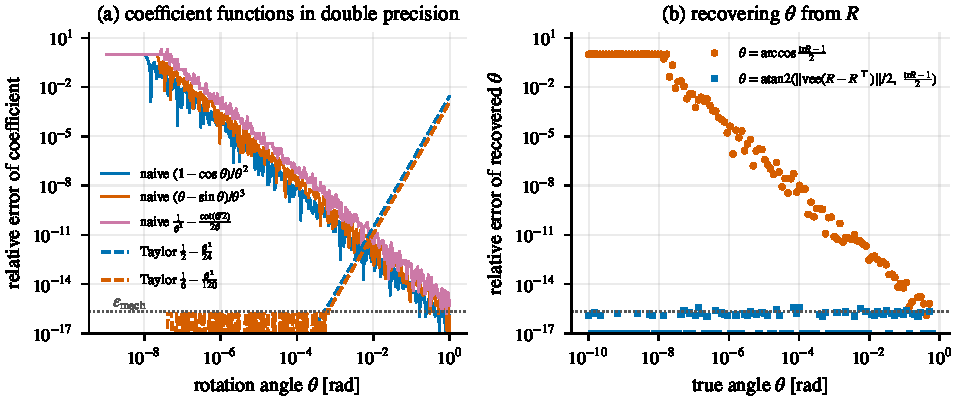
\includegraphics[width=\textwidth]{fig_taylor.pdf}
  \caption{(a) Relative error of the coefficient functions evaluated naively in double precision
  (solid) and with a two-term Taylor series (dashed), against a 60-digit reference. The naive error
  grows like $u/\theta^2$ as $\theta\to0$, and the truncation error of the series grows like $\theta^4$.
  (b) Recovering the angle from a rotation matrix: $\arccos$ loses accuracy like $u/\theta^2$ and
  returns exactly zero below $10^{-8}$, while the $\atantwo$ form is accurate to machine precision at
  every angle.}
  \label{fig:taylor}
\end{figure}

How much does the cancellation matter? It depends on what the coefficient multiplies. A coefficient
with absolute error $\epsilon_c$ that multiplies $\sx{\phi}^k$ contributes an error of about
$\epsilon_c\theta^k$ to the matrix. For $B$, $C$ and $D$, $\epsilon_c \approx u/\theta^2$, so:
\begin{center}\small
\begin{tabular}{@{}l l c l@{}}
\toprule
Function & cancelling coefficient & multiplies & naive absolute error \\
\midrule
$\Exp(\phi)$ & $B$ & $\sx{\phi}^2$ & $\approx u$ \quad (harmless) \\
$\Jr(\phi)$ & $B$ & $\sx{\phi}$ & $\approx u/\theta$ \quad (\textbf{harmful}: $3\times10^{-9}$ at $\theta = 10^{-8}$) \\
$\Jr(\phi)$ & $C$ & $\sx{\phi}^2$ & $\approx u$ \\
$\Jrinv(\phi)$ & $D$ & $\sx{\phi}^2$ & $\approx u$ \\
\bottomrule
\end{tabular}
\end{center}

\begin{keyidea}[why the Taylor branch exists, and how to choose its threshold]
Every function needs a guard against $0/0$. Beyond that, the branch matters for accuracy wherever a
cancelling coefficient multiplies a low power of $\sx{\phi}$, as in $\Jr$. To choose the threshold
$\theta_0$ and the number of terms, balance the two error curves of \cref{fig:taylor}(a): keeping terms
through $\theta^{2m}$ leaves a truncation error of order $\theta^{2m+2}$, and the exact formula has a
rounding error of order $u/\theta^2$. Below the crossing point use the series, above it the formula.
For two-term series ($m = 1$) the curves cross near $\theta \approx 3\times10^{-3}$, where both relative
errors are about $10^{-12}$; adding the $\theta^4$ term moves the crossing to larger angles and lowers
the error there. Remember to multiply by $\theta^k$ when translating a coefficient error into a matrix
error. Record the choice and this justification next to the code (Milestone 2).
\end{keyidea}

% ------------------------------------------------------------------------------
\section{The logarithm map}
\label{sec:log}

\begin{definition}[Logarithm map]
$\Log: \SO \to \R^3$ returns the rotation vector $\phi$ with $\|\phi\| \le \pi$ such that
$\Exp(\phi) = R$.
\end{definition}

For angles strictly between $0$ and $\pi$ the answer is unique. Combining the two equations of
\eqref{eq:trace-angle},
\begin{equation}
  \theta = \atantwo\!\Big( \tfrac12\big\|(R - R\T)\veeop\big\|,\ \tfrac12(\tr R - 1) \Big), \qquad
  \Log(R) = \frac{\theta}{2\sin\theta}\,(R - R\T)\veeop .
  \label{eq:Log}
\end{equation}
The $\atantwo$ form is essential. The common textbook formula $\theta = \arccos\big((\tr R - 1)/2\big)$ is
correct mathematically but numerically unstable near $\theta = 0$, where $\arccos$ has infinite slope,
and loses half the significant digits (\cref{fig:taylor}b). Three regimes need care in code.

\begin{enumerate}
  \item \textbf{Small angles.} $\theta/(2\sin\theta) \to \tfrac12$, so use
        $\Log(R) \approx \tfrac12(1 + \tfrac{\theta^2}{6})(R - R\T)\veeop$.
  \item \textbf{Generic angles.} Use \eqref{eq:Log} directly.
  \item \textbf{Angles near $\pi$.} $\sin\theta \to 0$ and $(R - R\T)\veeop = 2\sin\theta\,u$ vanishes, so
        the axis cannot be recovered from the skew-symmetric part. Use the symmetric part instead: from
        \eqref{eq:rodrigues}, $\tfrac12(R + R\T) = \cos\theta\,I + (1-\cos\theta)\,uu\T$, so
        $uu\T = \big(\tfrac12(R + R\T) - \cos\theta\, I\big)/(1 - \cos\theta)$. Take the column with the largest
        diagonal entry, normalize it to get $\pm u$, and fix the sign so that $u\T(R - R\T)\veeop \ge 0$.
\end{enumerate}

\begin{figure}[t]
\centering
\begin{tikzpicture}[scale=1.0]
  \fill[primarylight] (0,0) circle (2.0);
  \draw[primary, thick] (0,0) circle (2.0);
  \fill (0,0) circle (1.4pt) node[below right] {$I$};
  \draw[->, thick, plotorange] (0,0) -- (1.2,0.8) node[above right=-2pt] {$\phi$};
  \fill[plotgreen] (40:2.0) circle (2pt) node[above right] {$\pi u$};
  \fill[plotgreen] (220:2.0) circle (2pt) node[below left] {$-\pi u$};
  \draw[plotgreen, dashed, <->] (40:1.9) -- (220:1.9);
  \draw[->, plotpurple, thick] (-0.3,-1.2) .. controls (0.6,-1.4) and (1.4,-1.5) .. (330:2.0);
  \draw[->, plotpurple, thick] (150:2.0) .. controls (-1.2,0.6) .. (-0.6,0.4);
  \node[plotpurple, font=\footnotesize, align=left] at (3.6,-1.1) {a path leaving the ball\\re-enters at the\\antipodal point};
  \node[primary, font=\footnotesize] at (0,2.35) {$\|\phi\| \le \pi$};
\end{tikzpicture}
\caption{$\SO$ pictured as the ball of rotation vectors of radius $\pi$, with antipodal points on the
boundary identified ($\pi u$ and $-\pi u$ are the same rotation). $\Log$ is smooth inside the ball but
must jump when a rotation crosses $\theta = \pi$. Near the boundary a tiny change in $R$ can flip the
returned vector to the opposite side.}
\label{fig:so3-ball}
\end{figure}

\begin{remark}[why $\Log$ is ill-conditioned near $\pi$]
Near $\theta = \pi$ two different effects combine. Algebraically, the axis must be extracted from a
nearly vanishing skew-symmetric part, so the na\"ive formula amplifies rounding errors by
$1/\sin\theta$. Topologically, $\Log$ is discontinuous at $\theta = \pi$ (\cref{fig:so3-ball}): a
rotation by $\pi - \epsilon$ about $u$ and one by $\pi - \epsilon$ about $-u$ are close in $\SO$ but have
$\Log$ values $2\pi$ apart. No implementation can remove the second effect. In an estimator it rarely
matters, because $\Log$ is applied to \emph{differences} between nearby rotations, whose angles are
small. Milestone 2 nevertheless tests the near-$\pi$ regime, because a broken branch there produces
\code{NaN}.
\end{remark}

\paragraph{Quaternion logarithm.} For a unit quaternion $q = [w, v]$, first canonicalize to $w \ge 0$ (replace
$q$ by $-q$ if needed), then
\begin{equation}
  \Log_q(q) = 2\,\atantwo(\|v\|, w)\,\frac{v}{\|v\|}
  \ \approx\ \frac{2}{w}\Big(1 - \frac{\|v\|^2}{3w^2}\Big)\,v \quad\text{for small }\|v\|.
  \label{eq:Logq}
\end{equation}
Canonicalization guarantees $\|\Log_q(q)\| \le \pi$ and makes $\Log_q(q) = \Log_q(-q)$, so the double cover is
invisible to the estimator. The $\atantwo$ is well-conditioned at all angles, including near $\pi$ where
$w \approx 0$: the quaternion logarithm does not suffer the algebraic ill-conditioning of the matrix version.
The topological discontinuity at $\pi$ remains.

% ------------------------------------------------------------------------------
\section{The adjoint: moving a perturbation across a rotation}

\begin{proposition}[Adjoint of $\SO$]
\label{prop:adjoint}
For all $R \in \SO$ and $\phi \in \R^3$,
\begin{equation}
  R\,\Exp(\phi)\,R\T = \Exp(R\phi),
  \label{eq:adjoint}
\end{equation}
or equivalently $\Exp(\phi)\,R = R\,\Exp(R\T\phi)$ and $R\,\Exp(\phi) = \Exp(R\phi)\,R$.
\end{proposition}
\begin{proof}
By \eqref{eq:skew-rot}, $R\sx{\phi}R\T = \sx{R\phi}$. By property 4 of \cref{prop:matexp},
$R\exp(\sx{\phi})R\T = \exp(R\sx{\phi}R\T) = \exp(\sx{R\phi})$. The equivalent forms follow by
multiplying on the right or left by $R$ or $R\T$.
\end{proof}

The map $\phi \mapsto R\phi$ is the \emph{adjoint action} $\Ad_R$, which for $\SO$ is simply the rotation
matrix itself. Geometrically, a rotation about an axis $\phi$ expressed in one frame equals the rotation
about the same physical axis expressed in another frame. \Cref{eq:adjoint} is the single most used identity
in Jacobian derivations: it lets you slide a perturbation $\Exp(\delta)$ through other rotations until
it reaches the position the convention requires.

% ------------------------------------------------------------------------------
\section{Composition and the Baker--Campbell--Hausdorff formula}

Rotations about different axes do not commute, so $\Exp(a)\Exp(b) \neq \Exp(a + b)$ in general. The
Baker--Campbell--Hausdorff (BCH) formula quantifies the discrepancy. For matrices $X, Y$ near zero,
\begin{equation}
  \log\big(\exp X \exp Y\big) = X + Y + \tfrac12[X, Y] + \tfrac1{12}\big([X,[X,Y]] + [Y,[Y,X]]\big) + \cdots,
\end{equation}
where $[X, Y] = XY - YX$. For $\so$, \eqref{eq:skew-commutator} gives $[\sx{a}, \sx{b}] = \sx{a\times b}$, so
\begin{equation}
  \Log\big(\Exp(a)\Exp(b)\big) = a + b + \tfrac12\, a\times b
     + \tfrac1{12}\big( a\times(a\times b) + b\times(b\times a)\big) + \cdots .
  \label{eq:bch}
\end{equation}

\begin{proof}[Derivation of the second-order term]
Expand both exponentials to second order: $\exp X\exp Y = (I + X + \tfrac12X^2)(I + Y + \tfrac12Y^2) + O(3) = I + X + Y + \tfrac12X^2 + XY + \tfrac12Y^2 + O(3)$,
where $O(3)$ collects terms of third order in $X$ and $Y$. Write the result as $\exp Z$ with $Z = X + Y + Z_2 + O(3)$ and $Z_2$ of second order. Then
$\exp Z = I + Z + \tfrac12Z^2 + O(3) = I + X + Y + Z_2 + \tfrac12(X + Y)^2 + O(3)$. Comparing the two expansions,
$Z_2 = \tfrac12X^2 + XY + \tfrac12Y^2 - \tfrac12(X^2 + XY + YX + Y^2) = \tfrac12(XY - YX)$. The higher-order terms are obtained the same way, with
more patience; they involve only nested brackets, a theorem in itself.
\end{proof}
The first correction is second order. Two small rotations therefore compose approximately additively,
$\Exp(a)\Exp(b) \approx \Exp(a + b)$, with an error of order $\|a\|\|b\|$. When only one of them is small,
summing the BCH series in the large argument gives the two most important first-order formulas of
this chapter:
\begin{align}
  \Log\big(\Exp(\phi)\,\Exp(\delta)\big) &= \phi + \Jrinv(\phi)\,\delta + O(\|\delta\|^2), \label{eq:bch-right}\\
  \Log\big(\Exp(\delta)\,\Exp(\phi)\big) &= \phi + \Jlinv(\phi)\,\delta + O(\|\delta\|^2), \label{eq:bch-left}
\end{align}
with the Jacobians $\Jr$ and $\Jl$ defined in \cref{sec:jr}.

% ------------------------------------------------------------------------------
\section{Perturbations, \texorpdfstring{$\bplus$}{boxplus} and \texorpdfstring{$\bminus$}{boxminus}}
\label{sec:perturbations}
\label{sec:boxplus}

Let $\hat R$ be an estimate and $R$ the truth. There are two natural ways to write the small rotation
separating them:
\begin{equation}
  \underbrace{R = \hat R\,\Exp(\delta\theta_b)}_{\text{local (right) perturbation}}
  \qquad\qquad
  \underbrace{R = \Exp(\delta\theta_w)\,\hat R}_{\text{global (left) perturbation}} .
\end{equation}
By \cref{prop:adjoint} they describe the same error, related by $\delta\theta_w = \hat R\,\delta\theta_b$.
$\delta\theta_b$ is the error expressed in the estimated body frame, $\delta\theta_w$ the same error expressed in
the world frame. If $\delta\theta_b \sim \N(0, P_b)$, then $\delta\theta_w \sim \N(0, \hat R P_b \hat R\T)$.

\begin{figure}[t]
\centering
\begin{tikzpicture}[scale=1.0]
  % world frame
  \draw[frameaxis, black!60] (0,0) -- (1.1,0) node[right, font=\footnotesize] {$x_w$};
  \draw[frameaxis, black!60] (0,0) -- (0,1.1) node[above, font=\footnotesize] {$z_w$};
  \node[below left, font=\footnotesize] at (0,0) {$W$};
  % estimated and true body frames
  \begin{scope}[shift={(3.4,0.2)}]
    \begin{scope}[rotate=25]
      \draw[frameaxis, primary] (0,0) -- (1.5,0) node[right, font=\footnotesize] {$\hat x_b$};
      \draw[frameaxis, primary] (0,0) -- (0,1.5) node[above left=-2pt, font=\footnotesize] {$\hat z_b$};
    \end{scope}
    \begin{scope}[rotate=45]
      \draw[frameaxis, plotorange, dashed] (0,0) -- (1.5,0) node[above right=-1pt, font=\footnotesize] {$x_b$};
      \draw[frameaxis, plotorange, dashed] (0,0) -- (0,1.5) node[above left=-2pt, font=\footnotesize] {$z_b$};
    \end{scope}
    \draw[->, plotgreen, thick] (25:1.05) arc (25:45:1.05);
    \node[plotgreen, font=\footnotesize] at (35:1.45) {$\delta\theta_b$};
    \node[font=\footnotesize, align=center, below=4pt] at (0.4,0) {estimated frame $\hat R$ (solid)\\ and true frame $R$ (dashed)};
  \end{scope}
  % summary box
  \node[draw=conv, fill=convlight, rounded corners, align=left, font=\footnotesize, text width=5.4cm, anchor=west] at (6.6,0.6) {
    Local: $R = \hat R\Exp(\delta\theta_b)$ \textbf{(this project)}\\[2pt]
    Global: $R = \Exp(\delta\theta_w)\hat R$\\[2pt]
    Same error: $\delta\theta_w = \hat R\,\delta\theta_b$\\[2pt]
    Covariances: $P_w = \hat R P_b \hat R\T$};
\end{tikzpicture}
\caption{The local (right) perturbation measures the attitude error as a small rotation about the axes of
the \emph{estimated} body frame. The global (left) perturbation measures the same error about the world
axes.}
\label{fig:perturbations}
\end{figure}

Both conventions are mathematically valid and widely used, but they are not interchangeable. Every
Jacobian, covariance and residual depends on the choice. The project uses the local one for three
reasons.
\begin{enumerate}
  \item \textbf{It matches the sensor.} The gyroscope measures $\omega_b$ in the body frame and
        \eqref{eq:rdot} puts it on the right, so body-frame errors couple to body-frame quantities.
  \item \textbf{It is decoupled from global yaw.} The local attitude error dynamics
        (\cref{ch:errordyn}) depend on $\hat\omega$ and the biases but not on the absolute heading.
  \item \textbf{It is the convention of the standard ESKF reference~\cite{sola2017quaternion}}, which makes
        the literature easy to cross-check.
\end{enumerate}

\begin{convention}[retraction and local difference, AGENTS.md C4]
For the full state $x = (p, v, q, b_a, b_g, \{p_i, q_i\})$ and $\delta x \in \R^{15 + 6N}$:
\begin{align*}
  x = \hat x \bplus \delta x:&\quad p = \hat p + \delta p,\quad v = \hat v + \delta v,\quad
       q = \hat q\qprod\Exp_q(\delta\theta),\quad b = \hat b + \delta b, \\
  \delta x = x \bminus \hat x:&\quad \delta\theta = \Log_q(\hat q\inv\qprod q),\quad\text{all other blocks subtract.}
\end{align*}
Clone blocks follow the same rule. Every residual, Jacobian, injection and numerical-differentiation test
uses these two operators and nothing else.
\end{convention}

The operators satisfy the axioms that make them a consistent local parameterization:
\begin{equation}
  x \bplus 0 = x, \qquad (x \bplus \delta) \bminus x = \delta, \qquad x \bplus (y \bminus x) = y,
\end{equation}
the second for $\|\delta\theta\| < \pi$ and the third for any $y$. The state is a \emph{product manifold}
$\R^3\times\R^3\times\SO\times\R^3\times\R^3\times(\R^3\times\SO)^N$. Each factor has its own
$\bplus$, and the composite operator acts block-wise.

% ------------------------------------------------------------------------------
\section{Jacobians on manifolds}
\label{sec:jr}

\begin{definition}[Jacobian with respect to local perturbations]
\label{def:manifold-jacobian}
Let $f: \mathcal{M} \to \mathcal{N}$ map between manifolds with $\bplus$/$\bminus$ operators. Its
Jacobian at $x$ is the matrix
\begin{equation}
  J^f_x = \frac{\partial}{\partial\delta}\Big[ f(x\bplus\delta) \bminus f(x) \Big]_{\delta = 0},
  \qquad\text{so that}\qquad f(x\bplus\delta) = f(x)\bplus\big(J^f_x\,\delta + O(\|\delta\|^2)\big).
  \label{eq:manifold-jacobian}
\end{equation}
\end{definition}

When both spaces are vector spaces this is the ordinary Jacobian. The chain rule holds unchanged,
$J^{g\circ f}_x = J^g_{f(x)}\,J^f_x$, so complicated Jacobians are products of simple ones. The column
$j$ of $J^f_x$ is what a finite-difference test computes by perturbing direction $j$, which is how every
such Jacobian is verified.

\subsection{The right and left Jacobians of \texorpdfstring{$\SO$}{SO(3)}}

\begin{definition}[Right and left Jacobians]
The \emph{right Jacobian} $\Jr(\phi)$ is the Jacobian of $\Exp: \R^3 \to \SO$ with the local $\bminus$ on
$\SO$; the \emph{left Jacobian} $\Jl(\phi)$ uses the global one:
\begin{equation}
  \Exp(\phi + \delta) = \Exp(\phi)\,\Exp\big(\Jr(\phi)\,\delta\big) + O(\|\delta\|^2)
  = \Exp\big(\Jl(\phi)\,\delta\big)\,\Exp(\phi) + O(\|\delta\|^2).
  \label{eq:jr-def}
\end{equation}
\end{definition}

$\Jr(\phi)$ answers the question: if I change the rotation \emph{vector} $\phi$ by $\delta$, what small
\emph{body-frame} rotation does the rotation \emph{matrix} undergo? Only for $\phi = 0$ is the answer
$\delta$ itself.

\begin{theorem}[Closed forms]
\label{thm:jr}
With $\theta = \|\phi\|$,
\begin{align}
  \Jr(\phi) &= \int_0^1 \Exp(-s\phi)\,\dd s
             = I - \frac{1-\cos\theta}{\theta^2}\,\sx{\phi} + \frac{\theta - \sin\theta}{\theta^3}\,\sx{\phi}^2, \label{eq:jr}\\
  \Jrinv(\phi) &= I + \tfrac12\sx{\phi} + \Big(\frac{1}{\theta^2} - \frac{1 + \cos\theta}{2\theta\sin\theta}\Big)\sx{\phi}^2, \label{eq:jrinv}\\
  \Jl(\phi) &= \Jr(-\phi) = \Jr(\phi)\T = \Exp(\phi)\,\Jr(\phi), \qquad \Jlinv(\phi) = \Jrinv(-\phi). \label{eq:jl}
\end{align}
The coefficient in \eqref{eq:jrinv} equals $D(\theta) = \frac{1}{\theta^2} - \frac{\cot(\theta/2)}{2\theta}$,
which is finite at $\theta = \pi$ (where $D = 1/\pi^2$) and singular only at $\theta = 2\pi$.
\end{theorem}
\begin{proof}
\emph{Step 1: the derivative of the matrix exponential.} Let $K(t) = \exp\big(t(X + \epsilon Y)\big)$, which solves
$\dot K = (X + \epsilon Y)K$, $K(0) = I$. Its derivative with respect to $\epsilon$ at $\epsilon = 0$, $W(t) = \partial K/\partial\epsilon$, solves the equation obtained by
differentiating the ODE: $\dot W = XW + Y\exp(tX)$, $W(0) = 0$. This is a linear ODE with an input, so by variation of constants
(\cref{prop:stm}) $W(t) = \int_0^t\exp((t - s)X)\,Y\exp(sX)\,\dd s$. At $t = 1$, after substituting $s \to 1 - s$,
\begin{equation*}
  \frac{\dd}{\dd\epsilon}\exp(X + \epsilon Y)\Big|_{\epsilon=0} = \int_0^1 \exp(sX)\,Y\exp((1-s)X)\,\dd s .
\end{equation*}
\emph{Step 2: the integral form.} With $X = \sx{\phi}$ and $Y = \sx{\delta}$,
\begin{align*}
  \Exp(\phi)\inv\,\frac{\dd}{\dd\epsilon}\Exp(\phi + \epsilon\delta)\Big|_0
  &= \int_0^1 \Exp(-(1-s)\phi)\,\sx{\delta}\,\Exp((1-s)\phi)\,\dd s \\
  &= \Big[\int_0^1 \Exp(-s\phi)\,\dd s\ \delta\Big]_\times,
\end{align*}
using $R\sx{\delta}R\T = \sx{R\delta}$ with $R = \Exp(-(1-s)\phi)$ and substituting $s \to 1 - s$ again. Comparing with
$\Exp(\phi)\Exp(\epsilon\Jr\delta) = \Exp(\phi)(I + \epsilon\sx{\Jr\delta}) + O(\epsilon^2)$ gives $\Jr(\phi) = \int_0^1\Exp(-s\phi)\,\dd s$.

\emph{Step 3: the closed form.} With $u = \phi/\theta$, Rodrigues' formula gives
$\Exp(-s\phi) = I - \sin(s\theta)\sx{u} + (1 - \cos(s\theta))\sx{u}^2$. Integrating term by term, $\int_0^1\sin(s\theta)\,\dd s = (1 - \cos\theta)/\theta$ and
$\int_0^1(1 - \cos(s\theta))\,\dd s = 1 - \sin\theta/\theta$, so
$\Jr = I - \frac{1 - \cos\theta}{\theta}\sx{u} + \big(1 - \frac{\sin\theta}{\theta}\big)\sx{u}^2$; substituting $\sx{u} = \sx{\phi}/\theta$ gives \eqref{eq:jr}.

\emph{Step 4: the inverse.} Write $K = \sx{\phi}$, $\Jr = I - BK + CK^2$ with the coefficients $B$ and $C$ of \eqref{eq:jr}, and look for the inverse in the
same form, $I + aK + bK^2$. Multiplying out and reducing $K^3 = -\theta^2K$ and $K^4 = -\theta^2K^2$, the product equals $I$ exactly when
\begin{equation*}
  a - B + \theta^2(bB - aC) = 0, \qquad b - aB + C - \theta^2bC = 0 .
\end{equation*}
These two linear equations have the solution $a = \tfrac12$ and $b = D(\theta)$ (substitute the trigonometric expressions and simplify, or
check numerically), which is \eqref{eq:jrinv}; the identity $\frac{1+\cos\theta}{\sin\theta} = \cot\frac\theta2$ gives the form of $D$.

\emph{Step 5: the left Jacobian.} By \cref{prop:adjoint}, $\Exp(\phi)\Exp(\Jr\delta) = \Exp(\Exp(\phi)\Jr\delta)\Exp(\phi)$, so $\Jl = \Exp(\phi)\Jr$. Repeating
steps 1--3 with the perturbation on the left gives $\Jl = \int_0^1\Exp(s\phi)\,\dd s$, which is $\Jr(-\phi)$ and, since $\Exp(s\phi)\T = \Exp(-s\phi)$,
also $\Jr(\phi)\T$.
\end{proof}

The small-angle expansions are $\Jr(\phi) = I - \tfrac12\sx{\phi} + \tfrac16\sx{\phi}^2 + O(\theta^3)$ and
$\Jrinv(\phi) = I + \tfrac12\sx{\phi} + \tfrac1{12}\sx{\phi}^2 + O(\theta^4)$, with the coefficient series of
\eqref{eq:coeff-taylor}. Equations \eqref{eq:bch-right} and \eqref{eq:bch-left} follow from
\eqref{eq:jr-def} by inverting the relation.

\subsection{Elementary Jacobians}

\begin{table}[t]
\centering\small
\renewcommand{\arraystretch}{1.35}
\begin{tabular}{@{}l l l@{}}
\toprule
Function & Jacobian w.r.t.\ local perturbation & Note \\
\midrule
$f(R) = Rv$ & $\dfrac{\partial f}{\partial\delta\theta} = -R\sx{v}$ & rotate a body vector to world \\
$f(R) = R\T v$ & $\dfrac{\partial f}{\partial\delta\theta} = \sx{R\T v}$ & express a world vector in body \\
$f(R) = R\inv$ & $J = -R$ & output on $\SO$ (local) \\
$f(R_1, R_2) = R_1R_2$ & $J_{R_1} = R_2\T$, \quad $J_{R_2} = I$ & output on $\SO$ (local) \\
$f(\phi) = \Exp(\phi)$ & $J = \Jr(\phi)$ & vector to $\SO$ \\
$f(R) = \Log(R)$ & $J = \Jrinv(\Log R)$ & $\SO$ to vector \\
$f(\phi) = \Exp(\phi)\,v$ & $\dfrac{\partial f}{\partial\phi} = -\Exp(\phi)\sx{v}\Jr(\phi)$ & rotation vector acting on $v$ \\
$f(v) = Rv$ & $J = R$ & ordinary linear map \\
\bottomrule
\end{tabular}
\caption{Elementary Jacobians with respect to the local (right) perturbation $R \to R\Exp(\delta\theta)$. All
other Jacobians in these notes are products of these by the chain rule. Each entry has been checked
numerically by central differences.}
\label{tab:jacobians}
\end{table}

The entries of \cref{tab:jacobians} are derived in two or three lines each. The method is always the same:
\textbf{perturb, expand to first order, isolate the perturbation, and read off the coefficient.}

\begin{example}[Rotation action]
\label{ex:rotation-action}
For $f(R) = Rv$: $f(R\Exp(\delta\theta)) = R(I + \sx{\delta\theta})v + O(\|\delta\theta\|^2) = Rv + R\sx{\delta\theta}v$.
By \eqref{eq:skew-anticomm}, $\sx{\delta\theta}v = -\sx{v}\delta\theta$, so the Jacobian is $-R\sx{v}$.
\end{example}

\begin{example}[Inverse action]
For $f(R) = R\T v$: $(R\Exp(\delta\theta))\T v = \Exp(-\delta\theta)R\T v \approx (I - \sx{\delta\theta})R\T v =
R\T v + \sx{R\T v}\,\delta\theta$.
\end{example}

\begin{example}[Inverse and composition]
For $f(R) = R\inv$: $(R\Exp(\delta\theta))\inv = \Exp(-\delta\theta)R\T = R\T\Exp(-R\delta\theta)$ by
\eqref{eq:adjoint}, so $f(R)\inv f(R\bplus\delta\theta) = \Exp(-R\delta\theta)$ and the Jacobian is $-R$. For
$f = R_1R_2$ perturbed in $R_1$: $R_1\Exp(\delta\theta)R_2 = R_1R_2\Exp(R_2\T\delta\theta)$, so $J_{R_1} = R_2\T$.
Perturbing $R_2$ appends $\Exp(\delta\theta)$ directly, so $J_{R_2} = I$.
\end{example}

\begin{example}[Logarithm]
For $f(R) = \Log(R)$ with $\phi = \Log R$: $\Log(R\Exp(\delta\theta)) = \Log(\Exp(\phi)\Exp(\delta\theta)) \approx
\phi + \Jrinv(\phi)\delta\theta$ by \eqref{eq:bch-right}.
\end{example}

\begin{example}[A chain: a rotation vector acting on a vector]
For $f(\phi) = \Exp(\phi)v$, with $\phi$ an ordinary vector: $\Exp(\phi + \delta)v = \Exp(\phi)\Exp(\Jr\delta)v \approx \Exp(\phi)(v + \sx{\Jr\delta}v)
= \Exp(\phi)v - \Exp(\phi)\sx{v}\Jr(\phi)\delta$. This is the chain rule: the Jacobian of $\Exp$ (namely $\Jr$) followed by the Jacobian of the rotation action
(namely $-R\sx{v}$). It is the Jacobian one needs when a filter uses a rotation vector, rather than a perturbation of a rotation, as its state.
\end{example}

\begin{pitfall}[first-order expansions and products]
The expansion $\Exp(\delta\theta) \approx I + \sx{\delta\theta}$ is valid only when $\delta\theta$ is the
\emph{only} small quantity being differentiated. Products of two small quantities ($\sx{\delta\theta}\delta b$,
or $\sx{\delta\theta}n$ with noise $n$) are second order and are dropped. Large quantities such as the
nominal rotation, the angular rate or the specific force are never approximated.
\end{pitfall}

% ------------------------------------------------------------------------------
\section{Uncertainty on \texorpdfstring{$\SO$}{SO(3)}}

With the local perturbation, an uncertain attitude is the random rotation
\begin{equation}
  R = \hat R\,\Exp(\delta\theta), \qquad \delta\theta \sim \N(0, P_\theta),
\end{equation}
a ``Gaussian on the manifold'': the mean $\hat R$ lives on $\SO$ and the covariance $P_\theta$ lives in the
tangent space at $\hat R$, in body-frame coordinates. Its eigenvectors are body axes about which the
attitude is most or least certain. This distribution is not a Gaussian in any fixed coordinates of
$\SO$, which is exactly why it captures curved distributions such as the banana of \cref{fig:banana}
better than a Gaussian on Euler angles or matrix entries.

\paragraph{Propagation.} If $y = f(R)$ and $J$ is its manifold Jacobian, then to first order
$y = f(\hat R)\bplus\delta y$ with $\delta y \approx J\delta\theta \sim \N(0, JP_\theta J\T)$.

\paragraph{Compounding.} For independent uncertain rotations $R_1 = \hat R_1\Exp(\delta_1)$ and
$R_2 = \hat R_2\Exp(\delta_2)$, the composition is
$R_1R_2 = \hat R_1\hat R_2\Exp(\hat R_2\T\delta_1)\Exp(\delta_2) \approx \hat R_1\hat R_2\Exp(\hat R_2\T\delta_1 + \delta_2)$, so
\begin{equation}
  P_{12} = \hat R_2\T P_1\hat R_2 + P_2 .
\end{equation}

\begin{remark}[covariance entries rotate between axes]
\label{rem:cov-rotates}
Because $P_\theta$ is expressed in body axes, it changes when the body rotates even if no information is
gained or lost. Suppose the world yaw is uncertain and roll and pitch are perfectly known: in world
coordinates $P_w = \sigma^2 e_ze_z\T$. In body coordinates $P_b = \hat R\T P_w\hat R = \sigma^2 (\hat R\T e_z)(\hat R\T e_z)\T$.
If the vehicle rolls by $90^\circ$, the world vertical is the body $y$-axis, and the yaw uncertainty moves
from the $(z,z)$ to the $(y,y)$ entry of $P$. Individual diagonal entries of the attitude covariance
are therefore not monotonic during propagation (a Milestone 5 concept), although its trace and
eigenvalues behave as expected.
\end{remark}

\subsection{Averaging rotations}

\index{rotation averaging}
How should several noisy measurements $R_1, \dots, R_N$ of the same attitude be averaged? The arithmetic mean of matrices (or of
quaternions) is not a rotation, and the average of Euler angles is meaningless near wrap-around. The natural definition is the rotation that
minimizes the sum of squared tangent-space distances, $\bar R = \argmin\sum_i\|\Log(\bar R\T R_i)\|^2$. It is computed by the fixed-point iteration
\begin{equation}
  \bar R \gets \bar R\,\Exp\Big(\frac1N\sum_{i=1}^N\Log\big(\bar R\T R_i\big)\Big),
\end{equation}
which averages the residuals in the tangent space at the current estimate and moves the estimate by that average, exactly as one would
average vectors, but on the manifold. It converges in a few iterations when the rotations are within a few tens of degrees of each other.
A faster approximation projects the arithmetic mean $M = \frac1N\sum_iR_i$ onto $\SO$ with the SVD: if $M = U\Sigma V\T$, the closest rotation is
$U\diag(1, 1, \det(UV\T))V\T$ (the same construction as in \cref{sec:umeyama}).

% ------------------------------------------------------------------------------
\section{\texorpdfstring{$\SE$}{SE(3)} and the choice of state manifold}
\label{sec:se3}

The rigid transformations $T = \begin{bmatrix}R & p\\0 & 1\end{bmatrix}$ of \cref{ch:rotations} also form a Lie group, $\SE$, of dimension six.

\paragraph{Lie algebra.} Differentiating a curve $T(t)$ through the identity gives elements of the form
$\xi\hatop = \begin{bmatrix}\sx{\phi} & \rho\\ 0 & 0\end{bmatrix}$, parameterized by $\xi = (\rho, \phi) \in \R^6$: an angular velocity $\phi$ and a linear velocity $\rho$,
together a \emph{twist}.

\paragraph{Exponential.} The powers of $\xi\hatop$ are $\begin{bmatrix}K^k & K^{k-1}\rho\\0 & 0\end{bmatrix}$ for $k \ge 1$, with $K = \sx{\phi}$, so the exponential series gives
\begin{equation}
  \Exp(\rho, \phi) = \begin{bmatrix}\Exp(\phi) & \Jl(\phi)\,\rho \\ 0 & 1\end{bmatrix},
  \qquad \Jl(\phi) = \sum_{k\ge0}\frac{K^k}{(k + 1)!},
\end{equation}
where the series is the left Jacobian of \cref{thm:jr} (expand $\int_0^1\Exp(s\phi)\,\dd s$ term by term). Moving with a constant twist traces a
\emph{screw motion}: rotation about an axis combined with translation along it. The logarithm inverts the two blocks: $\phi = \Log(R)$ and
$\rho = \Jl(\phi)\inv p$.

\paragraph{Adjoint.} Conjugation $T\Exp(\xi)T\inv = \Exp(\Ad_T\xi)$ holds with the $6\times6$ matrix
\begin{equation}
  \Ad_T = \begin{bmatrix} R & \sx{p}R \\ 0 & R \end{bmatrix},
\end{equation}
obtained by multiplying out $T\xi\hatop T\inv$. It transforms twists between frames, and plays the same role for poses as $R$ does for rotation vectors.

\paragraph{Which manifold for the state?} Perturbing a pose on $\SE$, $T = \hat T\Exp(\delta\xi)$, expresses the translation error in the body frame
and couples it to the rotation error through $\Jl$. The project does \emph{not} do this: its state is the product manifold of
\cref{sec:boxplus}, in which the position error is a plain world-frame vector and the attitude error is a local rotation, independently.
To first order the two are related by a rotation of the translation error ($\delta p_w \approx \hat R\,\delta\rho$); they differ at second order. Both
choices are valid, but they produce different Jacobians and different covariances, and must never be mixed. A third choice, the
extended pose group $\mathrm{SE}_2(3)$ of $5\times5$ matrices $\begin{bmatrix}R & v & p\\0 & 1 & 0\\0 & 0 & 1\end{bmatrix}$ collecting attitude, velocity and
position, underlies the \emph{invariant} EKF, whose error dynamics have the striking property of not depending on the state at all
(\cref{ch:observability}).

% ------------------------------------------------------------------------------
\section{Verifying manifold Jacobians numerically}
\label{sec:numjac}

Every analytic Jacobian in the project is checked against a central difference built on the
$\bplus$/$\bminus$ operators (AGENTS.md E6). Column $j$ of the numerical Jacobian is
\begin{equation}
  J_{:,j} \approx \frac{ f(x\bplus h e_j) \bminus f(x\bplus(-h e_j)) }{2h},
  \qquad h \approx 10^{-6}.
  \label{eq:numjac}
\end{equation}
The central difference has truncation error $O(h^2)$ and rounding error $O(u/h)$
(\cref{sec:numdiff}), so analytic and numerical Jacobians should agree to about $10^{-8}$ relative
to the magnitude of the entries.

\begin{pitfall}[tests that cannot fail]
A Jacobian test evaluated at a trivial point proves little. At $R = I$, $R$ and $R\T$ are equal, so a
transpose bug is invisible; with zero angular rate, terms multiplied by $\hat\omega$ vanish; with zero
biases, bias-sign errors may hide. Always test at a random non-identity attitude, non-zero rates,
accelerations and biases, and ask of every test: \emph{would this still pass if I flipped the sign of
X?} A good habit is to temporarily break the analytic Jacobian and confirm that the test fails.
\end{pitfall}

\begin{projectlink}[Milestone 2]
\code{so3.hpp} implements \code{skew}, \code{Exp}/\code{Log}, \code{Exp\_q}/\code{Log\_q}, \code{J\_r} and
\code{J\_r\_inv} as derived here, and \code{numerical\_jacobian.hpp} implements \eqref{eq:numjac} generically
over $\bplus$/$\bminus$. The exit criteria test exactly the properties of this chapter: $\Exp(\phi) \in \SO$,
$\Log\circ\Exp = \mathrm{id}$ at zero, tiny, generic and near-$\pi$ angles, agreement of $\Exp_q$ and $\Exp$,
$\Log_q(q) = \Log_q(-q)$, the defining relation \eqref{eq:jr-def} of $\Jr$, and $\Jrinv\Jr = I$, all
without allocation.
\end{projectlink}

\begin{takeaways}
\begin{itemize}
  \item Attitude lives on the curved manifold $\SO$; its errors live in the flat tangent space $\R^3$.
        $\Exp$ and $\Log$ connect them.
  \item Compute angles with $\atantwo$, never with $\arccos$. Guard every coefficient function against
        $0/0$, and use Taylor branches wherever cancellation is amplified (notably in $\Jr$).
  \item Local (right) perturbation: $R = \hat R\Exp(\delta\theta)$, error in body axes. Global errors are
        $\hat R\,\delta\theta$.
  \item The adjoint identity $R\Exp(\phi)R\T = \Exp(R\phi)$ moves perturbations through rotations.
  \item $\Exp(\phi + \delta) \approx \Exp(\phi)\Exp(\Jr(\phi)\delta)$ and
        $\Log(\Exp(\phi)\Exp(\delta)) \approx \phi + \Jrinv(\phi)\delta$.
  \item Every project Jacobian is a chain-rule product of the entries of \cref{tab:jacobians}, and is
        verified by central differences at a non-trivial point.
\end{itemize}
\end{takeaways}

\begin{exercises}
  \item Show that $\so$ is closed under the commutator $[X, Y] = XY - YX$ and that
        $[\sx{a}, \sx{b}] = \sx{a\times b}$.
  \item Prove $\Exp(-\phi) = \Exp(\phi)\T$ and $\Exp(s\phi)\Exp(t\phi) = \Exp((s+t)\phi)$. Why does the second
        identity not contradict non-commutativity?
  \item Implement $\Log$ with both $\arccos$ and $\atantwo$ and reproduce \cref{fig:taylor}(b).
        Then construct a rotation within $10^{-6}$~rad of $\pi$ and test the near-$\pi$ branch.
  \item Using the coefficient series of \eqref{eq:coeff-taylor}, choose a threshold and a number of terms
        for $\Jr$ so that its absolute error stays below $10^{-14}$ for all $\theta \in [0, 0.1]$. Justify
        your choice with the error model of \cref{sec:taylor}.
  \item Derive the Jacobian of $f(R) = \Log(\hat R\T R)$ with respect to a local perturbation of $R$, and of
        $g(\hat R) = \Log(\hat R\T R)$ with respect to a local perturbation of $\hat R$. Evaluate both at
        $R = \hat R$. (These are the building blocks of attitude residuals.)
  \item Show that $\Jl(\phi) = \Exp(\phi)\Jr(\phi)$ and use it to prove \eqref{eq:bch-left} from
        \eqref{eq:bch-right}.
  \item A vehicle has attitude covariance $P_b = \diag(\sigma_r^2, \sigma_r^2, \sigma_y^2)$ in body axes while
        level. Compute $P_b$ after it pitches by $90^\circ$ with no new information, and interpret.
  \item Verify every row of \cref{tab:jacobians} with a 20-line Python script using central differences at
        a random point. Then flip one sign and confirm your script detects it.
\end{exercises}


\part{Estimation Theory}
\chapter{Estimation Fundamentals}
\label{ch:estimation}

\begin{objectives}
\begin{itemize}
  \item Define estimators, bias, variance and mean-square error.
  \item Derive linear and weighted least squares, the covariance of their estimates, and the Gauss--Markov theorem.
  \item Understand maximum likelihood, Fisher information and the Cram\'er--Rao bound: what ``information'' means.
  \item Derive the minimum mean-square-error and linear minimum mean-square-error estimators, and the orthogonality principle.
  \item Derive recursive least squares, the Kalman filter without dynamics.
  \item See that, for linear-Gaussian problems, all of these approaches give the same answer.
\end{itemize}
\end{objectives}

Before filtering, which estimates a changing state from a stream of measurements, comes \emph{estimation}: inferring unknown quantities
from noisy data. This chapter develops the classical theory. Its punchline is that several quite different philosophies (minimize squared
errors; maximize the probability of the data; compute the posterior mean) lead to the same formulas for linear-Gaussian problems, and those
formulas are the Kalman update.

% ==============================================================================
\section{Estimators and their errors}

\subsection{The setting}

An unknown quantity $x \in \R^n$ is to be inferred from data $z \in \R^m$ related to it by a model, typically
\begin{equation}
  z = h(x) + n, \qquad n \text{ random, zero mean, covariance } R .
\end{equation}
An \term{estimator} is a function $\hat x(z)$ of the data. Because the data are random, the estimate is random too, and its quality is judged
by the statistics of its \emph{error} $e = \hat x - x$ over repetitions of the experiment.

\begin{definition}[Bias, covariance and mean-square error]
The \term{bias} of an estimator is $b = \E[\hat x] - x$; it is \emph{unbiased} if $b = 0$. Its \term{mean-square error} matrix is
$\E[ee\T]$, and its scalar mean-square error is $\E[\|e\|^2] = \tr\E[ee\T]$.
\end{definition}

\begin{proposition}[Bias--variance decomposition]
$\E[ee\T] = \Cov(\hat x) + bb\T$, and hence $\E\|e\|^2 = \tr\Cov(\hat x) + \|b\|^2$.
\end{proposition}
\begin{proof}
Write $e = (\hat x - \E\hat x) + b$ and expand; the cross terms vanish because $\E[\hat x - \E\hat x] = 0$.
\end{proof}

An estimator can be accurate in two ways: by being unbiased, and by having a small covariance. A filter reports a covariance $P$ along with its
estimate, and a \emph{consistent} filter is one whose reported $P$ equals its actual mean-square error matrix (\cref{ch:consistency}).

% ==============================================================================
\section{Linear least squares}
\label{sec:linear-ls}

\subsection{The estimate}

Consider the linear model
\begin{equation}
  z = Hx + n, \qquad \E[n] = 0, \quad \Cov(n) = R,
  \label{eq:linear-model}
\end{equation}
with $H \in \R^{m\times n}$ of full column rank ($m \ge n$). The \term{weighted least-squares} (WLS) estimate minimizes the residuals weighted by the
inverse noise covariance, so that reliable measurements count more:
\begin{equation}
  \hat x = \argmin_x\ (z - Hx)\T R\inv(z - Hx) = \big(H\T R\inv H\big)\inv H\T R\inv z .
  \label{eq:wls}
\end{equation}
The formula comes from setting the gradient $-2H\T R\inv(z - Hx)$ to zero (\cref{sec:least-squares}).

\begin{proposition}[Statistics of the WLS estimate]
\label{prop:wls-cov}
The WLS estimate is unbiased, and its covariance is
\begin{equation}
  \Cov(\hat x) = \big(H\T R\inv H\big)\inv .
\end{equation}
\end{proposition}
\begin{proof}
Write $\hat x = Lz$ with $L = (H\T R\inv H)\inv H\T R\inv$. Then $LH = I$, so $\hat x = x + Ln$ and $\E\hat x = x$. By \cref{prop:affine},
$\Cov(\hat x) = LRL\T = (H\T R\inv H)\inv H\T R\inv RR\inv H(H\T R\inv H)\inv = (H\T R\inv H)\inv$.
\end{proof}

The matrix $H\T R\inv H$ is the \term{information} that the measurements carry about $x$, and its inverse is the uncertainty of the estimate.
Information from independent measurements adds: with stacked blocks $z_i = H_ix + n_i$ and block-diagonal $R$,
$H\T R\inv H = \sum_iH_i\T R_i\inv H_i$.

\begin{worked}[fitting a line]
A target moves along a line with unknown initial position $p_0$ and velocity $v$, and its position is measured at times $t_1, \dots, t_m$ with
independent noise of standard deviation $\sigma$: $z_i = p_0 + vt_i + n_i$. With $x = (p_0, v)$, $H$ has rows $(1, t_i)$ and $R = \sigma^2I$, so
\begin{equation*}
  H\T R\inv H = \frac{1}{\sigma^2}\begin{bmatrix} m & \sum t_i \\ \sum t_i & \sum t_i^2 \end{bmatrix}.
\end{equation*}
For $m$ measurements equally spaced over a duration $T$ with times centered on zero, the off-diagonal terms vanish and the velocity variance is
$\sigma^2/\sum t_i^2 \approx 12\sigma^2/(mT^2)$: velocity is determined more precisely when the measurements span a longer time, a first glimpse of how
dynamics turn position measurements into velocity information (\cref{fig:lsfit}).
\end{worked}

\begin{figure}[t]
  \centering
  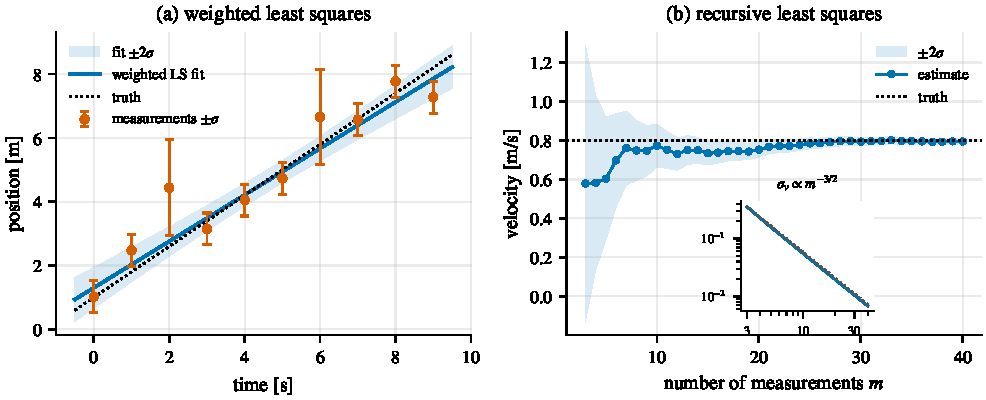
\includegraphics[width=\textwidth]{fig_lsfit.pdf}
  \caption{(a) Weighted least-squares fit of a line to noisy positions, with the $\pm2\sigma$ band of the fitted line from $(H\T R\inv H)\inv$.
  (b) Recursive least squares: the velocity estimate and its $\pm2\sigma$ bound as measurements arrive one at a time. The bound shrinks
  like $m^{-3/2}$ because later measurements also lengthen the time baseline.}
  \label{fig:lsfit}
\end{figure}

\subsection{The Gauss--Markov theorem}

Why weight by $R\inv$? Because it is the best possible linear choice.

\begin{theorem}[Gauss--Markov]
\label{thm:gauss-markov}
\index{Gauss--Markov theorem}
Among all linear unbiased estimators $\tilde x = Lz$ of $x$ in the model \eqref{eq:linear-model}, the WLS estimate \eqref{eq:wls} has the smallest
covariance: $\Cov(\tilde x) \succeq (H\T R\inv H)\inv$. It is the \term{best linear unbiased estimator} (BLUE).
\end{theorem}
\begin{proof}
Unbiasedness for every $x$ requires $LH = I$. Write $L = L_\star + D$ with $L_\star$ the WLS matrix; then $DH = 0$. The covariance is
$LRL\T = L_\star RL_\star\T + DRD\T + L_\star RD\T + DRL_\star\T$, and the cross terms vanish:
$L_\star RD\T = (H\T R\inv H)\inv H\T R\inv RD\T = (H\T R\inv H)\inv(DH)\T = 0$. So $\Cov(\tilde x) = \Cov(\hat x) + DRD\T \succeq \Cov(\hat x)$.
\end{proof}

The theorem needs no Gaussian assumption, only the first two moments of the noise. If the noise is Gaussian, more is true: WLS is the best of
\emph{all} unbiased estimators, linear or not, as the Cram\'er--Rao bound below shows.

% ==============================================================================
\section{Maximum likelihood}

\begin{definition}[Likelihood]
For a model with density $p(z\mid x)$, the \term{likelihood} of a value $x$ given observed data $z$ is $L(x) = p(z\mid x)$, viewed as a function of $x$.
The \term{maximum-likelihood} (ML) estimate maximizes it, equivalently minimizes the negative log-likelihood $-\log p(z\mid x)$.
\end{definition}

For Gaussian noise $n \sim \N(0, R)$ in $z = h(x) + n$,
\begin{equation}
  -\log p(z\mid x) = \tfrac12\big(z - h(x)\big)\T R\inv\big(z - h(x)\big) + \text{const},
\end{equation}
so ML estimation with Gaussian noise \emph{is} weighted least squares, linear or nonlinear. This is the justification of the least-squares
costs that pervade estimation, including the reprojection error of computer vision (\cref{ch:multiview}). For non-Gaussian noise, ML gives
other costs; heavy-tailed noise, for example, leads to the robust costs of \cref{ch:nlls}.

\subsection{Fisher information and the Cram\'er--Rao bound}

\begin{definition}[Fisher information]
\index{Fisher information}
For a model $p(z\mid x)$, the \term{Fisher information matrix} is
$\mathcal I(x) = \E\big[\nabla_x\log p(z\mid x)\,\nabla_x\log p(z\mid x)\T\big] = -\E\big[\nabla^2_x\log p(z\mid x)\big]$.
\end{definition}

The Fisher information measures how sharply the likelihood peaks around the true value: a likelihood that changes rapidly with $x$ pins $x$
down precisely. For the linear-Gaussian model, $\nabla^2_x\log p = -H\T R\inv H$, so $\mathcal I = H\T R\inv H$: the ``information matrix'' of WLS is the
Fisher information.

\begin{theorem}[Cram\'er--Rao lower bound]
\label{thm:crb}
\index{Cram\'er--Rao bound}
Under mild regularity conditions, every unbiased estimator satisfies $\Cov(\hat x) \succeq \mathcal I(x)\inv$.
\end{theorem}
\begin{proof}[Proof for a scalar parameter]
Let $s = \frac{\partial}{\partial x}\log p(z\mid x)$ (the \emph{score}). It has zero mean, since $\E[s] = \int\partial_xp\,\dd z = \partial_x\int p\,\dd z = 0$. Differentiating the
unbiasedness condition $\int\hat x(z)p(z\mid x)\,\dd z = x$ with respect to $x$ gives $\E[\hat x\,s] = 1$, hence $\Cov(\hat x, s) = 1$. By the
Cauchy--Schwarz inequality for covariances, $1 = \Cov(\hat x, s)^2 \le \Var(\hat x)\Var(s) = \Var(\hat x)\,\mathcal I(x)$.
\end{proof}

An unbiased estimator that attains the bound is \emph{efficient}. For the linear-Gaussian model, WLS attains it: $\Cov(\hat x) = (H\T R\inv H)\inv = \mathcal I\inv$.
No unbiased estimator can do better. This gives a precise meaning to the phrase used throughout these notes: \emph{information is inverse
covariance}, and independent measurements add their information.

% ==============================================================================
\section{Bayesian estimation}

\subsection{Priors and posteriors}

In the Bayesian view, the unknown $x$ is itself a random variable with a \emph{prior} density $p(x)$ that summarizes what is known before the
data. Bayes' rule gives the \emph{posterior} $p(x\mid z) \propto p(z\mid x)p(x)$, the complete description of what is known afterwards. Point estimates
summarize the posterior:
\begin{itemize}
  \item the \term{minimum mean-square error} (MMSE) estimate $\hat x = \E[x\mid z]$, the posterior mean;
  \item the \term{maximum a posteriori} (MAP) estimate, the posterior mode;
  \item and, ignoring the prior, the ML estimate.
\end{itemize}

\begin{theorem}[The conditional mean is optimal]
\label{thm:mmse}
Among all estimators $g(z)$, the conditional mean $\E[x\mid z]$ minimizes the Bayesian mean-square error $\E\|x - g(z)\|^2$, and indeed minimizes the
error matrix $\E[(x - g)(x - g)\T]$ in the Loewner order.
\end{theorem}
\begin{proof}
Fix $z$ and write $m = \E[x\mid z]$. For any value $g$, $\E\big[(x - g)(x - g)\T\mid z\big] = \Cov(x\mid z) + (m - g)(m - g)\T$ by the bias--variance decomposition
applied to the conditional distribution. The second term is PSD and vanishes exactly for $g = m$. Taking the expectation over $z$ preserves the
inequality.
\end{proof}

For a linear-Gaussian model the posterior is Gaussian (\cref{prop:map-ls}), so its mean and mode coincide: MMSE and MAP are the same estimate,
\begin{equation}
  \hat x = \big(P\inv + H\T R\inv H\big)\inv\big(P\inv\mu + H\T R\inv z\big), \qquad \Cov(x\mid z) = \big(P\inv + H\T R\inv H\big)\inv,
  \label{eq:bayes-linear}
\end{equation}
for a prior $\N(\mu, P)$. This is weighted least squares with one extra ``measurement'': the prior acts like a direct observation of $x$ with
value $\mu$ and covariance $P$. With an uninformative prior ($P\inv\to0$) it reduces to ML/WLS.

\subsection{Linear MMSE and the orthogonality principle}

The conditional mean can be hard to compute when distributions are not Gaussian. The best \emph{linear} (affine) estimator needs only means
and covariances.

\begin{theorem}[Linear minimum mean-square error estimator]
\label{thm:lmmse}
\index{linear MMSE estimator}\index{orthogonality principle}
Let $x$ and $z$ be random vectors with means $\mu_x$, $\mu_z$ and covariances $\Sigma_{xx}$, $\Sigma_{xz}$, $\Sigma_{zz} \succ 0$. Among estimators of the form
$\hat x = Az + b$, the mean-square error is minimized by
\begin{equation}
  \hat x = \mu_x + \Sigma_{xz}\Sigma_{zz}\inv(z - \mu_z),
  \qquad \E[(x - \hat x)(x - \hat x)\T] = \Sigma_{xx} - \Sigma_{xz}\Sigma_{zz}\inv\Sigma_{zx} .
\end{equation}
Its error is uncorrelated with the data: $\E\big[(x - \hat x)(z - \mu_z)\T\big] = 0$ (the \term{orthogonality principle}).
\end{theorem}
\begin{proof}
The error $e = x - Az - b$ has mean $\mu_x - A\mu_z - b$, which must vanish at the optimum (a non-zero mean only adds $bb\T$), so $b = \mu_x - A\mu_z$. Then
$e = (x - \mu_x) - A(z - \mu_z)$ and $\E[ee\T] = \Sigma_{xx} - A\Sigma_{zx} - \Sigma_{xz}A\T + A\Sigma_{zz}A\T$. Completing the square,
$\E[ee\T] = (A - A_\star)\Sigma_{zz}(A - A_\star)\T + \Sigma_{xx} - \Sigma_{xz}\Sigma_{zz}\inv\Sigma_{zx}$ with $A_\star = \Sigma_{xz}\Sigma_{zz}\inv$, which is minimal for $A = A_\star$. At the
optimum, $\E[e(z - \mu_z)\T] = \Sigma_{xz} - A_\star\Sigma_{zz} = 0$.
\end{proof}

The formulas are identical to Gaussian conditioning (\cref{thm:gauss-cond}): for jointly Gaussian variables the best linear estimator is the best
estimator of any kind, and for other distributions it is still the best linear one. The orthogonality principle has a geometric reading: the
estimate is the projection of $x$ onto the space of (affine) functions of the data, and the error is orthogonal to that space, exactly as a
least-squares residual is orthogonal to the column space (\cref{sec:least-squares}).

\paragraph{Application to the linear model.} For $z = Hx + n$ with prior mean $\mu$ and covariance $P$ for $x$, and noise uncorrelated with $x$:
$\mu_z = H\mu$, $\Sigma_{xz} = PH\T$, $\Sigma_{zz} = HPH\T + R$. \Cref{thm:lmmse} gives
\begin{equation}
  \hat x = \mu + K(z - H\mu), \qquad K = PH\T(HPH\T + R)\inv, \qquad \E[ee\T] = P - KHP .
  \label{eq:lmmse-update}
\end{equation}
This is the Kalman update (\cref{ch:kf}). By the Woodbury identity (\cref{thm:woodbury}) it equals \eqref{eq:bayes-linear}, but it requires
inverting an $m\times m$ matrix instead of an $n\times n$ one.

% ==============================================================================
\section{Recursive least squares}

Measurements often arrive one at a time, and recomputing \eqref{eq:wls} from scratch at each arrival would waste work. Since information adds,
the batch solution after $k$ measurements satisfies
\begin{equation}
  P_k\inv = P_{k-1}\inv + H_k\T R_k\inv H_k, \qquad P_k\inv\hat x_k = P_{k-1}\inv\hat x_{k-1} + H_k\T R_k\inv z_k,
\end{equation}
where $P_k$ is the covariance of $\hat x_k$. Rewriting this with the Woodbury identity gives the \term{recursive least squares} (RLS) update
\begin{equation}
  K_k = P_{k-1}H_k\T\big(H_kP_{k-1}H_k\T + R_k\big)\inv, \qquad
  \hat x_k = \hat x_{k-1} + K_k\big(z_k - H_k\hat x_{k-1}\big), \qquad
  P_k = (I - K_kH_k)P_{k-1} .
\end{equation}
Each step corrects the previous estimate by a gain times the \emph{innovation} $z_k - H_k\hat x_{k-1}$, the part of the new measurement that the old
estimate did not predict. It produces exactly the batch estimate at every step (\cref{fig:lsfit}b), at a cost that does not grow with the number
of measurements. RLS is the Kalman filter for a state that does not change; \cref{ch:kf} adds dynamics.

% ==============================================================================
\section{One answer, many derivations}

\begin{center}\small
\begin{tabularx}{\textwidth}{@{}l l >{\raggedright\arraybackslash}X@{}}
\toprule
Approach & Assumptions & Result for $z = Hx + n$ \\
\midrule
weighted least squares & second moments of the noise & $\hat x = (H\T R\inv H)\inv H\T R\inv z$ \\
Gauss--Markov (BLUE) & linear, unbiased & same \\
maximum likelihood & Gaussian noise & same \\
MAP / MMSE & Gaussian prior and noise & \eqref{eq:bayes-linear}: WLS with the prior as a measurement \\
linear MMSE & means and covariances only & \eqref{eq:lmmse-update}, equal to \eqref{eq:bayes-linear} \\
recursive LS & sequential data & same as batch, one measurement at a time \\
\bottomrule
\end{tabularx}
\end{center}

The Kalman filter inherits all of these interpretations. It is the exact Bayesian posterior for linear-Gaussian systems, the best linear
estimator when noises are merely uncorrelated, and a recursive least-squares solver. When models are nonlinear, these interpretations
separate, and the resulting approximations (\cref{ch:nlls,ch:nonlinear}) differ in which interpretation they try to preserve.

\begin{takeaways}
\begin{itemize}
  \item An estimator's error splits into bias and covariance: $\E[ee\T] = \Cov(\hat x) + bb\T$.
  \item Weighted least squares $\hat x = (H\T R\inv H)\inv H\T R\inv z$ has covariance $(H\T R\inv H)\inv$; information adds across independent measurements.
  \item Gauss--Markov: WLS with $R\inv$ weights is the best linear unbiased estimator.
  \item ML with Gaussian noise is least squares; the Fisher information bounds every unbiased estimator; information is inverse covariance.
  \item The conditional mean minimizes mean-square error; for Gaussians it equals the MAP estimate.
  \item The linear MMSE estimator $\mu + \Sigma_{xz}\Sigma_{zz}\inv(z - \mu_z)$ needs only second moments; its error is orthogonal to the data.
  \item Recursive least squares is the Kalman update without dynamics.
\end{itemize}
\end{takeaways}

\begin{exercises}
  \item Show that the sample mean of $m$ independent measurements of a scalar with variances $\sigma_i^2$ is not the BLUE unless all $\sigma_i$ are equal,
        and find the BLUE.
  \item For the line-fitting example with $m = 11$ measurements at $t = -5, \dots, 5$ and $\sigma = 1$, compute the covariance of $(p_0, v)$. How does it change
        if the times are $0, \dots, 10$? Interpret the off-diagonal term.
  \item Prove the matrix version of the Cram\'er--Rao bound for a linear-Gaussian model by computing $\nabla^2_x\log p$.
  \item Show that \eqref{eq:bayes-linear} and \eqref{eq:lmmse-update} agree, using \cref{thm:woodbury}.
  \item Derive the RLS update from the batch information form, and verify numerically that it reproduces the batch estimate at every step.
  \item Let $x \sim \mathcal U[-1, 1]$ and $z = x^3 + n$ with small Gaussian $n$. Compare the LMMSE estimate with the conditional mean, qualitatively. Why does
        the LMMSE estimate do poorly?
  \item A sensor reports a measurement with a bias $\beta$ that is not modeled. Show that the WLS estimate is biased by $(H\T R\inv H)\inv H\T R\inv\beta$, and explain
        why unmodeled biases are worse than large noise.
\end{exercises}
% Solutions to the exercises of Chapter 9.
\begin{solutions}
  \item The model is $z_i = x + n_i$, i.e.\ $H = \mathbf 1$ (a column of ones) and $R = \diag(\sigma_i^2)$. The WLS estimate is the BLUE
        (\cref{thm:gauss-markov}):
        \[
          \hat x = \big(\mathbf 1\T R\inv\mathbf 1\big)\inv\mathbf 1\T R\inv z = \frac{\sum_iz_i/\sigma_i^2}{\sum_i1/\sigma_i^2},
          \qquad \Var(\hat x) = \Big(\sum_i\frac{1}{\sigma_i^2}\Big)\inv,
        \]
        the inverse-variance weighted mean. The sample mean $\bar z = \frac1m\sum_iz_i$ is linear and unbiased with variance $\frac{1}{m^2}\sum_i\sigma_i^2$, and by the
        Cauchy--Schwarz inequality $\big(\sum_i\sigma_i^2\big)\big(\sum_i\sigma_i^{-2}\big) \ge m^2$, with equality only when all $\sigma_i$ are equal. So
        $\Var(\bar z) \ge \Var(\hat x)$, strictly unless the variances are equal: then (and only then) the two estimators coincide. One poor sensor can
        ruin a plain average; in the weighted one it simply counts for little.

  \item With $z_i = p_0 + vt_i + n_i$, $H$ has rows $(1, t_i)$ and $\Cov(\hat p_0, \hat v) = (H\T H)\inv$. For $t = -5, \dots, 5$, $\sum t_i = 0$ and $\sum t_i^2 = 110$, so
        \[
          (H\T H)\inv = \begin{bmatrix}11 & 0\\ 0 & 110\end{bmatrix}\inv = \diag\big(0.0909,\ 0.00909\big):
        \]
        $\sigma_{p_0} = 0.30$, $\sigma_v = 0.095$, uncorrelated. For $t = 0, \dots, 10$, $\sum t_i = 55$ and $\sum t_i^2 = 385$, and
        \[
          (H\T H)\inv = \frac{1}{1210}\begin{bmatrix}385 & -55\\ -55 & 11\end{bmatrix} = \begin{bmatrix}0.318 & -0.0455\\ -0.0455 & 0.00909\end{bmatrix}.
        \]
        The velocity variance is unchanged (it depends only on the spread of the times), but $p_0$ is now the value at the \emph{end} of the data,
        an extrapolation, with variance $3.5$ times larger and correlation $-0.85$ with $v$: a line that is too steep must start too low to pass
        through the data. The intercept is best determined at the centroid of the times, where the correlation vanishes.

  \item For $z = Hx + n$ with $n \sim \N(0, R)$, $\log p(z\mid x) = -\tfrac12(z - Hx)\T R\inv(z - Hx) + \text{const}$. Its gradient is
        $\nabla_x\log p = H\T R\inv(z - Hx)$ and its Hessian $\nabla_x^2\log p = -H\T R\inv H$, which does not depend on $z$, so
        $\mathcal I(x) = -\E[\nabla_x^2\log p] = H\T R\inv H$. (The outer-product definition agrees: $\E[H\T R\inv nn\T R\inv H] = H\T R\inv H$.) The matrix bound is
        proved like the scalar one: for an unbiased $\hat x$ and the score $s = \nabla_x\log p$, differentiating $\E[\hat x] = x$ gives $\Cov(\hat x, s) = I$, and
        the covariance matrix of $(\hat x, s)$,
        $\begin{bmatrix}\Cov(\hat x) & I\\ I & \mathcal I\end{bmatrix} \succeq 0$, has the PSD Schur complement $\Cov(\hat x) - \mathcal I\inv \succeq 0$ (Exercise 3.3's argument).
        WLS has covariance $(H\T R\inv H)\inv = \mathcal I\inv$ and attains the bound.

  \item Apply \cref{thm:woodbury} (as in Exercise 3.6) to the covariance of \eqref{eq:bayes-linear}:
        $(P\inv + H\T R\inv H)\inv = P - PH\T(HPH\T + R)\inv HP = P - KHP$ with $K = PH\T(HPH\T + R)\inv$, the covariance of \eqref{eq:lmmse-update}. For the mean,
        multiply out with this expression:
        \[
          (P - KHP)\big(P\inv\mu + H\T R\inv z\big) = \mu - KH\mu + \big(PH\T - KHPH\T\big)R\inv z .
        \]
        Since $K(HPH\T + R) = PH\T$, we have $PH\T - KHPH\T = KR$, so the last term is $Kz$, and the mean is $\mu + K(z - H\mu)$: the two forms agree.

  \item With prior $(\hat x_0, P_0)$, the batch estimate after $k$ measurements has information $P_k\inv = P_0\inv + \sum_{i\le k}H_i\T R_i\inv H_i$ and information
        vector $P_k\inv\hat x_k = P_0\inv\hat x_0 + \sum_{i\le k}H_i\T R_i\inv z_i$. Subtracting the expressions for $k - 1$ gives the recursion in information form
        stated in the chapter. Solving it for $\hat x_k$: $\hat x_k = P_k\big(P_{k-1}\inv\hat x_{k-1} + H_k\T R_k\inv z_k\big)$, and with
        $P_{k-1}\inv = P_k\inv - H_k\T R_k\inv H_k$ this is $\hat x_k = \hat x_{k-1} + P_kH_k\T R_k\inv(z_k - H_k\hat x_{k-1})$. Finally $P_kH_k\T R_k\inv = K_k$ (the
        push-through identity of Exercise 5.6) and $P_k = (I - K_kH_k)P_{k-1}$ by Woodbury. A numerical check with three unknowns, thirty scalar
        measurements of random variances and a weak prior: the RLS estimate and covariance agree with the batch solution after every
        measurement to $3\times10^{-12}$.

  \item The LMMSE estimate uses only second moments: with $\E[x] = \E[z] = 0$, $\Sigma_{xz} = \E[x^4] = \tfrac15$ and $\Sigma_{zz} = \E[x^6] + \sigma^2 = \tfrac17 + \sigma^2$,
        \[
          \hat x_{\mathrm{LMMSE}} = \frac{1/5}{1/7 + \sigma^2}\,z \approx 1.4\,z ,
        \]
        a straight line through a cube-root-shaped relation. The conditional mean $\E[x\mid z]$ follows the cube root, $\approx z^{1/3}$ wherever the noise is
        small compared with $z$. At $x = 0.5$ ($z = 0.125$) the LMMSE estimate is $0.17$, at $x = 0.9$ ($z = 0.73$) it is $1.02$, outside the support of $x$;
        the conditional mean gives $0.50$ and $0.90$. Overall, for $\sigma = 0.01$, the LMMSE root-mean-square error is $0.23$ against $0.075$ for the
        conditional mean (computed numerically). LMMSE does poorly because the dependence of $z$ on $x$ is strongly nonlinear: the best straight line
        fits neither small nor large values. This is the limitation the EKF inherits, mitigated by linearizing locally around the current estimate
        rather than globally.

  \item With $z = Hx + n + \beta$, the estimate $\hat x = Lz$ with $L = (H\T R\inv H)\inv H\T R\inv$ satisfies $LH = I$, so
        \[
          \hat x - x = Ln + L\beta, \qquad \E[\hat x] - x = (H\T R\inv H)\inv H\T R\inv\beta .
        \]
        The noise term has zero mean and covariance $(H\T R\inv H)\inv$, which shrinks as measurements accumulate ($\propto 1/m$ for $m$ comparable measurements).
        The bias term does not shrink: a constant offset in every measurement is averaged, not cancelled. The estimate therefore converges,
        with ever-smaller reported covariance, to the wrong value, and the filter becomes overconfident. Large noise is honest: it is in $R$, so it
        makes the covariance large. An unmodeled bias is invisible to the covariance and, if $\beta$ lies in the range of $H$, invisible in the residuals
        too, because it is indistinguishable from a different $x$. The cure is to model the bias as a state (\cref{ch:processes}), which is exactly
        why IMU biases are part of the filter state.
\end{solutions}


\chapter[Nonlinear Least Squares and Optimization]{Nonlinear Least Squares\\ and Optimization}
\label{ch:nlls}
\chaptermark{Nonlinear Least Squares} % short running header

\begin{objectives}
\begin{itemize}
  \item Formulate estimation problems with nonlinear models as nonlinear least-squares problems.
  \item Derive Newton, Gauss--Newton and Levenberg--Marquardt iterations, and understand when each converges.
  \item Optimize over manifolds such as $\SO$ by iterating in the tangent space.
  \item Make least squares robust to outliers with M-estimators and iteratively reweighted least squares.
  \item Exploit the structure of problems with poses and landmarks: the Schur complement and marginalization.
  \item See that an extended Kalman update is one Gauss--Newton step, the bridge between filtering and optimization.
\end{itemize}
\end{objectives}

Most measurement models in VIO are nonlinear: projections divide by depth, rotations enter through trigonometric functions. Maximum
likelihood with Gaussian noise then becomes a \emph{nonlinear} least-squares problem with no closed-form solution. This chapter develops the
iterative methods that solve such problems. They are used directly in this project for triangulation, and they explain what the extended
Kalman filter and the MSCKF are doing.

% ==============================================================================
\section{The problem}

Given residual functions $r_i(x)$ (measurement minus prediction) with noise covariances $R_i$, the maximum-likelihood estimate minimizes
\begin{equation}
  F(x) = \frac12\sum_i r_i(x)\T R_i\inv r_i(x) = \frac12\,r(x)\T W\,r(x),
  \label{eq:nlls}
\end{equation}
where $r$ stacks the residuals and $W = \blkdiag(R_i\inv)$. Examples in these notes:
\begin{itemize}
  \item \emph{Triangulation}: find a 3D point minimizing the reprojection errors in several images (\cref{ch:multiview}).
  \item \emph{Relative pose}: find the motion between two images that best explains point correspondences.
  \item \emph{Bundle adjustment}: find all camera poses and all points at once.
  \item \emph{Sliding-window VIO}: find a window of states minimizing visual and inertial residuals together.
\end{itemize}
Writing $W = L\T L$ (for instance $L$ the inverse of a Cholesky factor of the noise covariance) and replacing $r$ by $Lr$ \emph{whitens} the residuals,
so that $W = I$. We do this silently when convenient.

% ==============================================================================
\section{Descent methods}

The gradient and Hessian of $F$ follow from the chain rule. With $J = \partial r/\partial x$,
\begin{equation}
  \nabla F = J\T Wr, \qquad \nabla^2F = J\T WJ + \sum_k(Wr)_k\,\nabla^2r_k .
  \label{eq:nlls-derivatives}
\end{equation}

\paragraph{Gradient descent.} Step downhill, $x \gets x - \alpha\nabla F$, with a step length $\alpha$ chosen by a line search. It always makes progress for small
enough $\alpha$, but it ignores curvature and zig-zags slowly along narrow valleys.

\paragraph{Newton's method.} Minimize the quadratic Taylor model $F(x + \delta) \approx F + \nabla F\T\delta + \tfrac12\delta\T\nabla^2F\,\delta$ exactly:
\begin{equation}
  \nabla^2F\,\delta = -\nabla F .
\end{equation}
Near a minimum with positive-definite Hessian, Newton's method converges \emph{quadratically}: the number of correct digits roughly doubles each
iteration. But it needs second derivatives of every residual, and far from the minimum the Hessian may not be positive definite, in which case the
step can go uphill.

% ==============================================================================
\section{Gauss--Newton}
\label{sec:gauss-newton}

\index{Gauss--Newton method}
Least-squares problems allow a better compromise. Linearize the \emph{residuals} rather than the cost: $r(x + \delta) \approx r + J\delta$. The cost then
becomes a linear least-squares problem in $\delta$,
\begin{equation}
  \min_\delta\ \tfrac12\|r + J\delta\|_W^2
  \quad\Longrightarrow\quad
  \big(J\T WJ\big)\,\delta = -J\T Wr,
  \label{eq:gn-step}
\end{equation}
the \term{Gauss--Newton} step. Comparing with \eqref{eq:nlls-derivatives}, Gauss--Newton is Newton's method with the second term of the Hessian dropped.
That term is small when the residuals are small at the solution, or when the residuals are nearly linear, which is the common case for
well-modeled sensors. Then Gauss--Newton converges almost as fast as Newton, without second derivatives. The approximate Hessian $J\T WJ$ is
always positive semi-definite, so the step is always a descent direction (if $J$ has full column rank).

\begin{algorithm}[h]
\caption{Gauss--Newton}
\label{alg:gauss-newton}
\begin{algorithmic}[1]
\Require initial guess $x$, residual function $r(x)$ and its Jacobian $J(x)$
\Repeat
  \State evaluate $r$ and $J$ at $x$
  \State solve $(J\T WJ)\,\delta = -J\T Wr$ \Comment{Cholesky of $J\T WJ$, or QR of the whitened $J$}
  \State $x \gets x + \delta$
\Until{$\|\delta\|$ or the decrease of $F$ is below a tolerance}
\end{algorithmic}
\end{algorithm}

The linear system is the normal equation of a linear least-squares problem, so all the numerical advice of \cref{sec:least-squares} applies: for
small, well-conditioned problems Cholesky of $J\T WJ$ is fine; for ill-conditioned ones, QR of the whitened Jacobian is safer.

\paragraph{When Gauss--Newton fails.} With a poor initial guess, large residuals or strong nonlinearity, the linear model can be a bad
approximation, and a full step can increase the cost. If $J\T WJ$ is singular, some direction is not determined by the data (a \emph{gauge freedom}
or an unobservable direction), and the step is undefined.

\section{Levenberg--Marquardt}

\index{Levenberg--Marquardt method}
The \term{Levenberg--Marquardt} (LM) method damps the Gauss--Newton step:
\begin{equation}
  \big(J\T WJ + \lambda D\big)\,\delta = -J\T Wr, \qquad \lambda \ge 0,
\end{equation}
with $D = I$ or $D = \diag(J\T WJ)$. For $\lambda\to0$ it is Gauss--Newton; for large $\lambda$ the step becomes a short gradient-descent step. The damping is
adapted to how well the linear model predicted the actual change of cost. With the \emph{gain ratio}
\begin{equation}
  \rho = \frac{F(x) - F(x + \delta)}{F(x) - \tfrac12\|r + J\delta\|_W^2},
\end{equation}
a step with $\rho$ close to one is accepted and $\lambda$ decreased (trust the model more), while a step with small or negative $\rho$ is rejected and
$\lambda$ increased. LM is equivalent to a \emph{trust-region} method that restricts the step to a region where the linearization is trusted. It is
the default solver of most computer-vision and robotics libraries.

\begin{figure}[t]
  \centering
  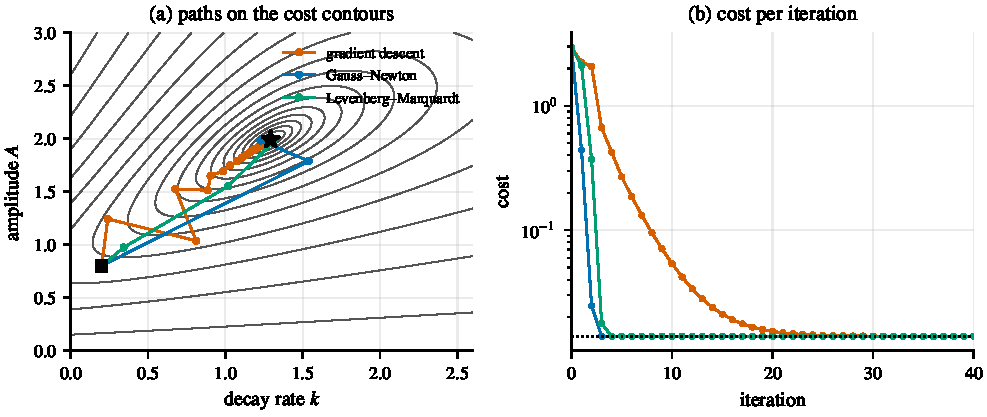
\includegraphics[width=\textwidth]{fig_gn_lm.pdf}
  \caption{Fitting the decay rate and amplitude of an exponential to noisy data. (a) Paths of gradient descent, Gauss--Newton and
  Levenberg--Marquardt on the contours of the cost, from the same starting point. (b) Cost versus iteration. Gradient descent crawls along the
  curved valley; Gauss--Newton and LM reach the minimum in a handful of iterations.}
  \label{fig:gn-lm}
\end{figure}

\section{Uncertainty of the solution}

At the minimum $\hat x$, the cost is approximately quadratic, $F(\hat x + \delta) \approx F(\hat x) + \tfrac12\delta\T(J\T WJ)\delta$, and with $W$ equal to the inverse
noise covariance the estimate has approximately the WLS covariance of the linearized problem (\cref{prop:wls-cov}):
\begin{equation}
  \Cov(\hat x) \approx \big(J\T WJ\big)\inv\Big|_{\hat x} .
\end{equation}
This is the \emph{Laplace approximation}: the posterior is replaced by a Gaussian fitted to its peak. It is accurate when the problem is nearly
linear over the region of uncertainty. A triangulated point, for example, gets a covariance from the Jacobians of its reprojection errors.

% ==============================================================================
\section{Optimization on manifolds}
\label{sec:manifold-opt}

When the unknown includes rotations, $x + \delta$ is replaced by the retraction $x\bplus\delta$ of \cref{ch:lie}. Linearize the residual in the tangent space,
$r(x\bplus\delta) \approx r(x) + J\delta$ with $J$ the manifold Jacobian (\cref{def:manifold-jacobian}), solve the same Gauss--Newton equation for $\delta$, and
update $x \gets x\bplus\delta$. The step is computed in a flat space and applied on the curved one, so the iterate never leaves the manifold and no
constraint ever needs enforcing. Covariances are then expressed in the tangent space at the solution, exactly as in a filter.

\begin{example}[Rotation averaging as Gauss--Newton]
Average rotations $R_1, \dots, R_N$ (\cref{ch:lie}) by minimizing $\tfrac12\sum_i\|r_i\|^2$ with $r_i(\bar R) = \Log(\bar R\T R_i)$. Perturbing
$\bar R\bplus\delta = \bar R\Exp(\delta)$ gives $r_i = \Log(\Exp(-\delta)\bar R\T R_i) \approx r_i(\bar R) - \Jlinv(r_i)\,\delta$ (\cref{eq:bch-left}). For small residuals
$\Jlinv \approx I$, so $J_i \approx -I$, and the Gauss--Newton step is $\delta = \frac1N\sum_ir_i$: exactly the averaging iteration of \cref{ch:lie}.
\end{example}

% ==============================================================================
\section{Robust estimation}
\label{sec:robust}

\subsection{Outliers break least squares}

A squared cost gives enormous influence to large residuals: a single wrong measurement, far from the others, can drag a least-squares estimate
arbitrarily far. Real data contain such \term{outliers}: misassociated features, reflections, moving objects. Two defenses exist: detect and
remove them (gating, RANSAC), or reduce their influence with a robust cost.

\subsection{M-estimators}

\index{M-estimator}\index{robust kernel}
An \term{M-estimator} replaces the quadratic by a function $\rho$ of the whitened residual norm $s_i = \|r_i\|_{R_i\inv}$:
\begin{equation}
  \min_x\ \sum_i\rho(s_i) .
\end{equation}

\begin{center}\small
\begin{tabular}{@{}l l l@{}}
\toprule
Kernel & $\rho(s)$ & weight $w(s) = \rho'(s)/s$ \\
\midrule
least squares & $\tfrac12s^2$ & $1$ \\
Huber & $\tfrac12s^2$ for $s\le c$;\ \ $c(s - \tfrac c2)$ otherwise & $1$ for $s \le c$;\ \ $c/s$ otherwise \\
Cauchy & $\tfrac{c^2}2\log(1 + s^2/c^2)$ & $1/(1 + s^2/c^2)$ \\
Tukey & $\tfrac{c^2}6\big(1 - (1 - s^2/c^2)^3\big)$ for $s \le c$;\ \ $c^2/6$ otherwise & $(1 - s^2/c^2)^2$ for $s \le c$;\ \ $0$ otherwise \\
\bottomrule
\end{tabular}
\end{center}

\begin{figure}[t]
  \centering
  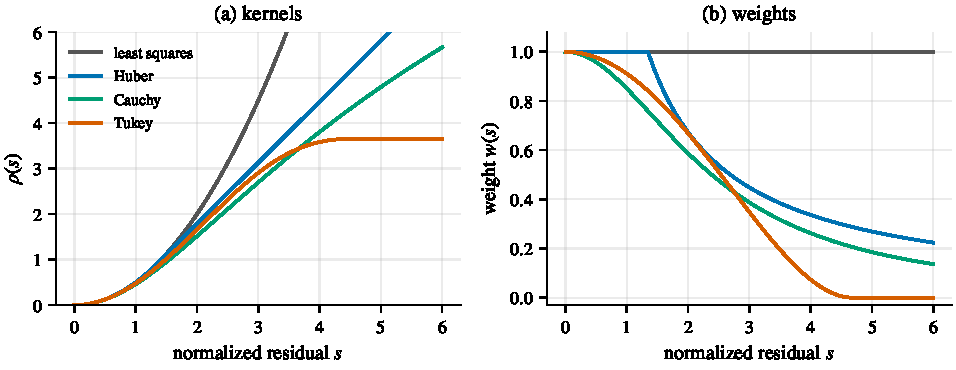
\includegraphics[width=\textwidth]{fig_robust_kernels.pdf}
  \caption{Robust kernels (left) and their weights (right) as functions of the normalized residual, for $c = 1.345$ (Huber), $2.385$ (Cauchy) and
  $4.685$ (Tukey). Huber grows linearly instead of quadratically for large residuals; Cauchy grows logarithmically; Tukey ignores residuals beyond
  $c$ entirely.}
  \label{fig:robust-kernels}
\end{figure}

The derivative $\psi = \rho'$ (the \emph{influence function}) measures how hard a residual pulls on the estimate: unbounded and linear for least squares,
bounded for Huber, decreasing to zero for Cauchy and Tukey (\cref{fig:robust-kernels}). The constants $c$ trade efficiency on clean Gaussian data against
robustness; the values in the figure keep 95\% of the efficiency of least squares on Gaussian noise.

\subsection{Iteratively reweighted least squares}

Setting the gradient of $\sum_i\rho(s_i)$ to zero gives $\sum_iw(s_i)J_i\T R_i\inv r_i = 0$ with $w(s) = \rho'(s)/s$: the normal equations of a \emph{weighted}
least-squares problem whose weights depend on the residuals. \emph{Iteratively reweighted least squares} (IRLS) alternates: compute the weights
from the current residuals, take a Gauss--Newton step with those weights, repeat. Outliers receive small weights and stop dominating. Robust
kernels need a reasonable initial guess, because with large initial errors every residual looks like an outlier; RANSAC (\cref{ch:multiview})
provides such guesses.

Gating, used in filters, is the hard-decision version of the same idea: a measurement whose normalized residual exceeds a threshold gets weight
zero, all others weight one, a ``truncated quadratic'' kernel.

% ==============================================================================
\section{Structure: poses, landmarks and the Schur complement}
\label{sec:schur-ba}

Many estimation problems have two kinds of unknowns. In bundle adjustment, the cameras $c$ and the landmarks $l$; in VIO smoothing, the states in
a window and the features. Each residual involves one camera and one landmark, so the normal equations have a special block structure:
\begin{equation}
  \begin{bmatrix} A & B \\ B\T & C \end{bmatrix}\begin{bmatrix}\delta c\\ \delta l\end{bmatrix} = \begin{bmatrix}g_c\\ g_l\end{bmatrix},
\end{equation}
where $C$, the landmark block of $J\T WJ$, is block diagonal with one $3\times3$ block per landmark (no residual involves two landmarks). Inverting $C$ is
therefore cheap. Eliminating the landmarks with the Schur complement (\cref{sec:schur}),
\begin{equation}
  \big(A - BC\inv B\T\big)\,\delta c = g_c - BC\inv g_l, \qquad \delta l = C\inv(g_l - B\T\delta c),
  \label{eq:reduced-camera-system}
\end{equation}
leaves a \emph{reduced camera system} whose size depends only on the number of cameras, often a hundred times smaller than the full problem.

\begin{figure}[t]
  \centering
  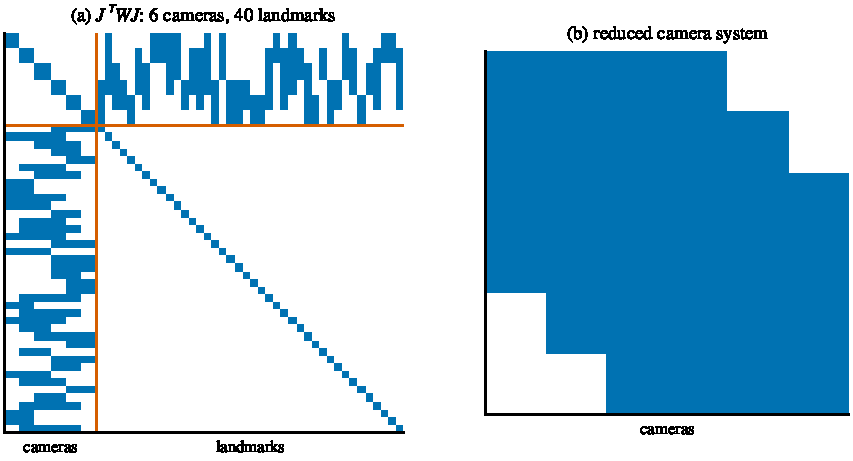
\includegraphics[width=\textwidth]{fig_ba_sparsity.pdf}
  \caption{Sparsity of the normal-equation matrix $J\T WJ$ for a toy bundle adjustment with 6 cameras and 40 landmarks (left), and of the reduced camera
  system after eliminating the landmarks (right). The landmark block is block-diagonal and cheap to eliminate; the reduced system is small but dense.}
  \label{fig:ba-sparsity}
\end{figure}

The same operation has a probabilistic meaning. $J\T WJ$ is the information matrix of the linearized problem, and the Schur complement is
\emph{marginalization in information form} (\cref{thm:gauss-cond}): the reduced system is the information that the measurements carry about the
cameras alone, after the landmarks have been integrated out. Sliding-window estimators use exactly this to discard old states, keeping their
information as a Gaussian prior on the remaining ones; the price is \emph{fill-in}, since the reduced matrix is dense (\cref{fig:ba-sparsity}). The
MSCKF performs the same elimination of each landmark, by a different algebraic route: the left-nullspace projection (\cref{ch:msckfupdate}).

% ==============================================================================
\section{Filtering as optimization}
\label{sec:filter-gn}

\begin{proposition}[The EKF update is one Gauss--Newton step]
\label{prop:ekf-gn}
\index{iterated EKF}
Consider the MAP cost of one measurement $z = h(x) + n$, $n \sim \N(0, R)$, with prior $\N(\mu, P)$:
\begin{equation*}
  F(x) = \tfrac12\|x - \mu\|^2_{P\inv} + \tfrac12\|z - h(x)\|^2_{R\inv}.
\end{equation*}
One Gauss--Newton step from $x = \mu$ gives $x^+ = \mu + K(z - h(\mu))$ with $K = PH\T(HPH\T + R)\inv$ and $H = \partial h/\partial x|_\mu$: the extended
Kalman update (\cref{ch:nonlinear}).
\end{proposition}
\begin{proof}
The stacked residual is $r(x) = \big(L_P(x - \mu),\ L_R(h(x) - z)\big)$ with $L_P\T L_P = P\inv$ and $L_R\T L_R = R\inv$. At $x = \mu$, $r = (0,\ L_R(h(\mu) - z))$ and
$J = (L_P,\ L_RH)$, so the Gauss--Newton equation \eqref{eq:gn-step} reads $(P\inv + H\T R\inv H)\delta = H\T R\inv(z - h(\mu))$. By the Woodbury identity,
$(P\inv + H\T R\inv H)\inv H\T R\inv = PH\T(HPH\T + R)\inv = K$.
\end{proof}

Iterating the Gauss--Newton step, re-linearizing $h$ at each new estimate while keeping the prior term, gives the \emph{iterated} EKF, which
handles strong measurement nonlinearities better. Sliding-window smoothers go further and re-linearize past measurements as well. The MSCKF update
is one Gauss--Newton step of a sliding-window problem whose landmarks have been eliminated (\cref{ch:msckfupdate}): filtering and optimization
are two ends of one spectrum, distinguished by how often they re-linearize and which variables they keep.

\begin{takeaways}
\begin{itemize}
  \item ML with Gaussian noise means minimizing $\tfrac12 r\T Wr$; the gradient is $J\T Wr$ and $J\T WJ$ approximates the Hessian.
  \item Gauss--Newton solves $(J\T WJ)\delta = -J\T Wr$ repeatedly; it converges fast when residuals are small or nearly linear.
  \item Levenberg--Marquardt damps the step adaptively and is robust to poor initial guesses.
  \item On manifolds, compute the step in the tangent space and apply it with $\bplus$.
  \item $(J\T WJ)\inv$ at the optimum approximates the covariance of the estimate.
  \item Robust kernels bound the influence of outliers; IRLS solves them; gating is the hard version.
  \item Eliminating landmarks with the Schur complement is marginalization in information form.
  \item An EKF update is one Gauss--Newton step on the MAP cost; iterating gives the iterated EKF.
\end{itemize}
\end{takeaways}

\begin{exercises}
  \item Derive the gradient and Hessian \eqref{eq:nlls-derivatives} of the least-squares cost.
  \item Implement Gauss--Newton and LM for fitting $y = ae^{-bt}$ to noisy data and reproduce \cref{fig:gn-lm}. Start from a poor initial guess and compare
        robustness.
  \item Show that for a zero-residual problem Gauss--Newton converges quadratically near the solution.
  \item Fit a line to data containing 20\% gross outliers with least squares, Huber IRLS and Cauchy IRLS. Compare the results.
  \item Implement the Schur-complement solution \eqref{eq:reduced-camera-system} for a random sparse problem and verify that it matches the full solve.
  \item Prove that the reduced camera system equals the inverse of the camera block of $(J\T WJ)\inv$, and interpret this as marginalization.
  \item Write out one iteration of the iterated EKF and show that it reduces to the standard EKF update after the first iteration.
\end{exercises}

\chapter{Linear Dynamical Systems}
\label{ch:linsys}

\begin{objectives}
\begin{itemize}
  \item Write physical systems in continuous- and discrete-time state-space form.
  \item Discretize deterministic inputs and white process noise exactly and approximately, including Van Loan's method.
  \item Understand stability, and why inertial errors grow polynomially.
  \item Define observability, test it with the observability matrix, and compute unobservable directions.
  \item Understand what observability means for the covariance of a Kalman filter.
\end{itemize}
\end{objectives}

The Kalman filter is built on a linear state-space model. This chapter collects the linear systems theory it needs: how to write a model, how
to turn a continuous-time model into the discrete-time form a computer processes, and how to decide whether the measurements can determine the
state at all.

% ==============================================================================
\section{State-space models}

A continuous-time linear \term{state-space model} has the form
\begin{equation}
  \dot x(t) = F(t)\,x(t) + B(t)\,u(t) + G(t)\,w(t), \qquad z(t) = H(t)\,x(t) + n(t),
  \label{eq:ct-model}
\end{equation}
with state $x$, known input $u$, white process noise $w$ (density $Q_c$), measurement $z$ and measurement noise $n$. The state is the smallest set of
numbers whose present value, together with future inputs and noises, determines the future. Its discrete-time counterpart is
\begin{equation}
  x_{k+1} = \Phi_k\,x_k + \Gamma_k\,u_k + w_k, \qquad z_k = H_k\,x_k + n_k,
  \qquad w_k \sim \N(0, Q_k),\ n_k \sim \N(0, R_k).
  \label{eq:dt-model}
\end{equation}

\begin{example}[Models used in these notes]
\label{ex:state-models}
\begin{itemize}
  \item \emph{Constant velocity}: $x = (p, v)$, $\dot p = v$, $\dot v = w$ (white acceleration). $F = \begin{bmatrix}0 & 1\\0 & 0\end{bmatrix}$, $G = \begin{bmatrix}0\\1\end{bmatrix}$.
  \item \emph{Random-walk bias}: $\dot b = w_b$. $F = 0$, $G = 1$.
  \item \emph{Inertial error model} (one axis, preview of \cref{ch:errordyn}): $\delta\dot p = \delta v$, $\delta\dot v = g\,\delta\theta - \delta b_a - n_a$,
        $\delta\dot\theta = -\delta b_g - n_g$, plus random-walk biases. A chain of integrators driven by noise.
\end{itemize}
\end{example}

The discrete-time solution follows by repeated substitution:
\begin{equation}
  x_k = \Phi(k, 0)\,x_0 + \sum_{j=0}^{k-1}\Phi(k, j+1)\big(\Gamma_ju_j + w_j\big), \qquad \Phi(k, j) = \Phi_{k-1}\Phi_{k-2}\cdots\Phi_j,
\end{equation}
the discrete analog of the variation-of-constants formula (\cref{prop:stm}).

% ==============================================================================
\section{Discretization}
\label{sec:discretization}

Physical laws are continuous, computers are discrete. Over a step $\Dt$ in which $F$, $B$ and $G$ are constant, the solution of \eqref{eq:ct-model}
(\cref{thm:lti-solution}) is
\begin{equation}
  x(t + \Dt) = \underbrace{e^{F\Dt}}_{\Phi}\,x(t) + \int_0^\Dt e^{Fs}B\,u(t + \Dt - s)\,\dd s + \underbrace{\int_0^\Dt e^{Fs}G\,w(t + \Dt - s)\,\dd s}_{w_k},
\end{equation}
which has exactly the discrete form \eqref{eq:dt-model}.

\paragraph{Deterministic inputs.} If the input is held constant over the step (a \emph{zero-order hold}, which is what a sampled IMU reading
means), the input term is $\Gamma u_k$ with $\Gamma = \int_0^\Dt e^{Fs}\,\dd s\,B$. Both $\Phi$ and $\Gamma$ come from one matrix exponential,
\begin{equation}
  \exp\!\Big(\begin{bmatrix} F & B \\ 0 & 0\end{bmatrix}\Dt\Big) = \begin{bmatrix} \Phi & \Gamma \\ 0 & I\end{bmatrix},
\end{equation}
which can be verified by noting that both sides solve the same matrix ODE in $\Dt$.

\paragraph{Process noise.} The discrete noise $w_k$ is a weighted integral of white noise, so it is zero-mean Gaussian with covariance (by the
same calculation as in \cref{prop:lyapunov})
\begin{equation}
  Q_d = \int_0^\Dt e^{Fs}\,GQ_cG\T\,e^{F\T s}\,\dd s .
  \label{eq:qd-exact}
\end{equation}

\subsection{Approximations}

Expanding to first order in $\Dt$ gives the approximations used by most real-time filters and frozen in AGENTS.md F2:
\begin{equation}
  \Phi \approx I + F\Dt, \qquad Q_d \approx GQ_cG\T\,\Dt .
  \label{eq:disc-first-order}
\end{equation}
Both are accurate to $O(\Dt^2)$ per step. The units confirm the second: a noise density $\sigma_a$ in $\mathrm{m/s^2/\sqrt{Hz}}$ gives $\sigma_a^2\Dt$ in
$\mathrm{m^2/s^2}$, a velocity variance. A second-order option adds $\tfrac12F^2\Dt^2$ to $\Phi$ and $\tfrac12(FGQ_cG\T + GQ_cG\T F\T)\Dt^2$ to $Q_d$.

\begin{example}[Double integrator]
\label{ex:double-integrator-qd}
For position and velocity driven by white acceleration of density $\sigma$, $F = \begin{bmatrix}0&1\\0&0\end{bmatrix}$, $G = \begin{bmatrix}0\\1\end{bmatrix}$, $Q_c = \sigma^2$.
\Cref{ex:double-integrator} gives $e^{Fs}G = [s;\ 1]$, so \eqref{eq:qd-exact} evaluates exactly to
\begin{equation}
  Q_d = \sigma^2\begin{bmatrix} \Dt^3/3 & \Dt^2/2 \\ \Dt^2/2 & \Dt \end{bmatrix}.
\end{equation}
The first-order approximation $Q_d \approx \diag(0, \sigma^2\Dt)$ puts no noise on position within a single step. Yet after $n$ steps of exact $\Phi$, the
accumulated position variance is $\sum_{k=1}^{n} (k\Dt)^2\sigma^2\Dt \to \sigma^2 t^3/3$ as $\Dt\to0$ (a Riemann sum), which is the exact answer of
\cref{prop:integrated-noise}. The per-step error of the approximation does not accumulate into a wrong growth law; it only introduces an $O(\Dt)$
relative error, negligible at 200~Hz.
\end{example}

\subsection{Van Loan's method}

When higher accuracy is wanted, \eqref{eq:qd-exact} can be computed exactly with a single matrix exponential~\cite{vanloan1978}.

\begin{proposition}[Van Loan]
\label{prop:vanloan}
\index{Van Loan's method}
Let $C = \exp\!\Big(\begin{bmatrix} -F & GQ_cG\T \\ 0 & F\T \end{bmatrix}\Dt\Big) = \begin{bmatrix} C_{11} & C_{12} \\ 0 & C_{22}\end{bmatrix}$. Then
$\Phi = C_{22}\T$ and $Q_d = \Phi\, C_{12}$.
\end{proposition}
\begin{proof}
For a block upper-triangular generator, the diagonal blocks of the exponential are the exponentials of the diagonal blocks, so $C_{22} = e^{F\T\Dt}$.
The off-diagonal block, as a function of $\Dt$, satisfies $\dot C_{12} = -FC_{12} + GQ_cG\T C_{22}$ with $C_{12}(0) = 0$, whose solution (variation of constants)
is $C_{12} = \int_0^\Dt e^{-F(\Dt - s)}\,GQ_cG\T\,e^{F\T s}\,\dd s$. Multiplying by $\Phi = e^{F\Dt}$ on the left, and using
$e^{F\Dt}e^{-F(\Dt - s)} = e^{Fs}$, gives $\Phi C_{12} = \int_0^\Dt e^{Fs}\,GQ_cG\T\,e^{F\T s}\,\dd s$, which is \eqref{eq:qd-exact}.
\end{proof}

For the 15-state inertial error model this costs a $30\times30$ matrix exponential per step, too expensive at 200~Hz but an excellent test oracle for the
closed forms of \cref{ch:errordyn}.

% ==============================================================================
\section{Stability}

A linear time-invariant system is \emph{stable} if its free response decays. For $\dot x = Fx$ the modes are $e^{\lambda_it}$ (\cref{thm:lti-solution}), so the
system is asymptotically stable when all eigenvalues of $F$ have negative real parts. For $x_{k+1} = \Phi x_k$ the modes are $\lambda_i^k$, so all eigenvalues of
$\Phi$ must lie strictly inside the unit circle; the two conditions correspond through $\lambda_\Phi = e^{\lambda_F\Dt}$.

Integrators have eigenvalues at zero (continuous) or one (discrete): they are \emph{marginally} stable. A single integrator holds its state; a chain of
integrators (a nilpotent $F$) makes initial errors grow \emph{polynomially}, like $t$, $t^2$, $t^3$. The error dynamics of inertial navigation are of this
kind (\cref{ex:state-models}), which is why IMU errors grow polynomially rather than exponentially, and why they never stop growing without aiding.

% ==============================================================================
\section{Observability}
\label{sec:observability-linear}

\subsection{Definition and the observability matrix}

\begin{definition}[Observability]
\index{observability}
A system is \term{observable} if the initial state $x_0$ can be determined from the inputs and the noise-free outputs over a finite time.
\end{definition}

Because the inputs are known, their contribution to the outputs can be subtracted, so observability depends only on $(\Phi, H)$. For a discrete
time-invariant system without noise, $z_k = H\Phi^kx_0$. Stacking the first $n$ outputs,
\begin{equation}
  \begin{bmatrix} z_0 \\ z_1 \\ \vdots \\ z_{n-1}\end{bmatrix} = \underbrace{\begin{bmatrix} H \\ H\Phi \\ \vdots \\ H\Phi^{n-1}\end{bmatrix}}_{\mathcal O}x_0 .
\end{equation}

\begin{theorem}[Observability rank test]
\label{thm:obs-rank}
\index{observability matrix}
The system is observable if and only if the \term{observability matrix} $\mathcal O$ has rank $n$. Its nullspace is the \term{unobservable subspace}: the
initial states that produce identically zero output forever.
\end{theorem}
\begin{proof}
If $\mathcal O$ has full column rank, $x_0$ is the unique solution of the stacked equations. If $\mathcal Ox_0 = 0$ for some $x_0 \ne 0$, then $H\Phi^kx_0 = 0$ for
$k < n$, and by the Cayley--Hamilton theorem ($\Phi^n$ is a linear combination of $I, \Phi, \dots, \Phi^{n-1}$) also for all $k \ge n$; such an $x_0$ is
indistinguishable from zero. More outputs never add rank beyond the first $n$.
\end{proof}

The unobservable subspace is invariant under $\Phi$: an unobservable error stays unobservable as the system evolves. For time-varying systems, the
same reasoning gives $\mathcal O = [H_0;\ H_1\Phi(1, 0);\ H_2\Phi(2, 0);\ \dots]$, and observability can depend on the trajectory, a fact that matters
greatly for VIO (\cref{ch:observability}).

\subsection{Examples}

\begin{example}[Position versus velocity measurements]
For the discretized constant-velocity model, $\Phi = \begin{bmatrix}1 & \Dt\\0 & 1\end{bmatrix}$.
\begin{itemize}
  \item Measuring position, $H = [1\ \ 0]$: $\mathcal O = \begin{bmatrix}1 & 0\\1 & \Dt\end{bmatrix}$ has rank 2. Velocity is observable, through the change of position.
  \item Measuring velocity, $H = [0\ \ 1]$: $\mathcal O = \begin{bmatrix}0 & 1\\0 & 1\end{bmatrix}$ has rank 1, with nullspace $(1, 0)$. Position is unobservable: shifting the whole
        trajectory changes no measurement. This is dead reckoning in one line.
\end{itemize}
\end{example}

\begin{example}[A bias that looks like the state]
Let $x = (p, b)$ with $\dot p = 0$, $\dot b = 0$ and $z = p + b$. Then $H = [1\ \ 1]$, $\Phi = I$, and $\mathcal O = \begin{bmatrix}1 & 1\\1 & 1\end{bmatrix}$ has nullspace $(1, -1)$: a
change of position compensated by an opposite change of bias is invisible. A sensor bias can be estimated only if something else breaks this
symmetry. In inertial navigation that something is motion: an accelerometer bias becomes separable from tilt once the vehicle rotates
(\cref{ch:strapdown}).
\end{example}

\begin{example}[An IMU along a line]
Let $x = (p, v, b_a)$ with $\dot p = v$, $\dot v = a_m - b_a$ ($a_m$ known) and $\dot b_a = 0$, and measure $p$. In continuous time,
$F = \begin{bmatrix}0&1&0\\0&0&-1\\0&0&0\end{bmatrix}$ and $H = [1\ 0\ 0]$, and the continuous-time observability matrix $[H;\ HF;\ HF^2]$ is
$\begin{bmatrix}1&0&0\\0&1&0\\0&0&-1\end{bmatrix}$, of full rank. Position measurements reveal velocity (one differentiation) and the accelerometer bias (two
differentiations): the reason a pose sensor makes all IMU states observable in Milestone 6.
\end{example}

\subsection{Duality and controllability}

The dual notion, \emph{controllability}, asks whether the inputs (or noises) can drive the state anywhere; its test matrix is
$[\Gamma,\ \Phi\Gamma,\ \dots,\ \Phi^{n-1}\Gamma]$, and $(\Phi, \Gamma)$ is controllable exactly when $(\Phi\T, \Gamma\T)$ is observable. For a Kalman filter,
controllability by the process noise means that every state is continually excited by noise, which keeps the filter from becoming certain
of anything and ignoring new data.

\subsection{What observability means for a filter}

For a time-invariant system that is observable from its measurements and controllable from its process noise, the Kalman filter covariance
converges to a unique, bounded steady state, whatever the initial covariance (\cref{ch:kf}). Along unobservable directions there is no such
bound: the covariance there can only grow with process noise or stay at its prior value, because no measurement reduces it. A filter must
respect this. If its linearized model makes an unobservable direction appear observable, it will \emph{reduce} the covariance along that direction
without justification, and become overconfident. This is precisely what happens to the standard EKF in VIO (\cref{ch:observability}).

\begin{takeaways}
\begin{itemize}
  \item State-space models collect everything needed to predict the future; discrete models follow from continuous ones by integrating over
        a step.
  \item $\Phi = e^{F\Dt}$, $Q_d = \int e^{Fs}GQ_cG\T e^{F\T s}\dd s$; to first order $\Phi \approx I + F\Dt$ and $Q_d \approx GQ_cG\T\Dt$. Van Loan computes both exactly.
  \item Chains of integrators are marginally stable: their errors grow polynomially.
  \item Observability: $\mathcal O = [H;\ H\Phi;\ \dots]$ must have full rank; its nullspace contains the directions the outputs cannot see.
  \item A filter may reduce uncertainty only in observable directions.
\end{itemize}
\end{takeaways}

\begin{exercises}
  \item Write the mass-spring-damper $m\ddot y + c\dot y + ky = u$ in state-space form and find its eigenvalues. When is it stable?
  \item Compute $\Gamma$ for the double integrator with a zero-order-hold acceleration input, and interpret its entries.
  \item Verify \cref{prop:vanloan} numerically for the double integrator.
  \item Find the unobservable subspace of the constant-velocity model with measurements of $p_1 - p_2$ for two independent targets.
  \item Show that the continuous-time system $\dot x = Fx$, $z = Hx$ is observable if and only if $[H;\ HF;\ \dots;\ HF^{n-1}]$ has full rank.
  \item A gyroscope measures $\omega + b_g$, and an inclinometer measures the integrated angle. Is the gyro bias observable? What if the inclinometer
        is replaced by a second gyroscope?
\end{exercises}
% Solutions to the exercises of Chapter 11.
\begin{solutions}
  \item With $x = (y, \dot y)$,
        \[
          \dot x = \begin{bmatrix}0 & 1\\ -k/m & -c/m\end{bmatrix}x + \begin{bmatrix}0\\ 1/m\end{bmatrix}u .
        \]
        The characteristic polynomial is $\lambda^2 + (c/m)\lambda + k/m$, so $\lambda = \big(-c \pm \sqrt{c^2 - 4km}\big)/2m$, or
        $\lambda = -\zeta\omega_n \pm \omega_n\sqrt{\zeta^2 - 1}$ with $\omega_n = \sqrt{k/m}$ and $\zeta = c/(2\sqrt{km})$. For $m > 0$ both roots have negative real parts
        exactly when $c > 0$ and $k > 0$ (a quadratic with positive coefficients): the system is asymptotically stable. Underdamped ($\zeta < 1$) it
        oscillates with decaying amplitude; with $c = 0$ the eigenvalues $\pm i\omega_n$ lie on the imaginary axis and the system is only marginally stable;
        with $k < 0$ (a negative spring) one eigenvalue is positive and it is unstable. This is the accelerometer model of \cref{ch:imu}.

  \item With $F = \begin{bmatrix}0 & 1\\0 & 0\end{bmatrix}$ and $B = \begin{bmatrix}0\\1\end{bmatrix}$, $e^{Fs}B = \begin{bmatrix}s\\1\end{bmatrix}$ (\cref{ex:double-integrator}), so
        \[
          \Gamma = \int_0^\Dt e^{Fs}B\,\dd s = \begin{bmatrix}\Dt^2/2\\ \Dt\end{bmatrix}.
        \]
        An acceleration $a$ held constant over the step adds $\tfrac12a\Dt^2$ to the position and $a\Dt$ to the velocity: the familiar kinematics of constant
        acceleration, exact for a zero-order-hold input. The block exponential $\exp\big(\begin{bmatrix}F & B\\0 & 0\end{bmatrix}\Dt\big)$, whose generator is nilpotent
        ($3\times3$ with cube zero), gives the same result after two terms.

  \item With $\Dt = 0.1$ and $\sigma = 1$, \code{scipy.linalg.expm} of $\begin{bmatrix}-F & GQ_cG\T\\ 0 & F\T\end{bmatrix}\Dt$ gives
        \[
          \Phi = C_{22}\T = \begin{bmatrix}1 & 0.1\\0 & 1\end{bmatrix}, \qquad
          Q_d = \Phi C_{12} = \begin{bmatrix}3.333\times10^{-4} & 5\times10^{-3}\\ 5\times10^{-3} & 0.1\end{bmatrix},
        \]
        which equals the exact $\sigma^2\begin{bmatrix}\Dt^3/3 & \Dt^2/2\\ \Dt^2/2 & \Dt\end{bmatrix}$ of \cref{ex:double-integrator-qd} to $10^{-18}$.

  \item With $x = (p_1, v_1, p_2, v_2)$, $\Phi = \blkdiag\big(\begin{bmatrix}1 & \Dt\\0 & 1\end{bmatrix}, \begin{bmatrix}1 & \Dt\\0 & 1\end{bmatrix}\big)$ and $H = [1\ \ 0\ \ {-1}\ \ 0]$, the rows
        of the observability matrix are $H\Phi^k = [1\ \ k\Dt\ \ {-1}\ \ {-k\Dt}]$, which span a two-dimensional space: $\rank\mathcal O = 2$. The unobservable subspace
        is
        \[
          \nullsp(\mathcal O) = \mathrm{span}\{(1, 0, 1, 0),\ (0, 1, 0, 1)\}:
        \]
        a common translation and a common velocity of both targets. The relative measurement reveals the relative position and the relative
        velocity, but nothing about where the pair is or how it moves as a whole: the one-dimensional version of the unobservable global position of
        VIO.

  \item For $\dot x = Fx$, $z(t) = He^{Ft}x_0$, and the derivatives of the output at $t = 0$ are $z^{(k)}(0) = HF^kx_0$. If $\mathcal O_c = [H;\ HF;\ \dots;\ HF^{n-1}]$ has
        full column rank, the noise-free output over any interval determines these derivatives and hence $x_0 = (\mathcal O_c\T\mathcal O_c)\inv\mathcal O_c\T
        (z(0), \dot z(0), \dots)$. Conversely, if $\mathcal O_cx_0 = 0$ for some $x_0 \ne 0$, then $HF^kx_0 = 0$ for $k < n$, and by the Cayley--Hamilton theorem for all
        $k$, so $z(t) = \sum_k\frac{t^k}{k!}HF^kx_0 = 0$ for all $t$: $x_0$ produces the same output as the zero state, and the system is unobservable.

  \item Let the state be $(\theta, b_g)$ with the gyro reading $\omega_m$ as the known input: $\dot\theta = \omega_m - b_g$, $\dot b_g = 0$, and the inclinometer
        measures $z = \theta$. Then $F = \begin{bmatrix}0 & -1\\0 & 0\end{bmatrix}$, $H = [1\ \ 0]$, and $\mathcal O = \begin{bmatrix}1 & 0\\0 & -1\end{bmatrix}$ has full rank: the bias is
        observable, as the slope of the difference between the integrated gyro and the inclinometer. With a second gyroscope instead, the two
        readings are $\omega + b_1$ and $\omega + b_2$ of the same unknown rate $\omega$. Shifting $\omega \to \omega + c$, $b_1 \to b_1 - c$, $b_2 \to b_2 - c$ leaves both readings
        unchanged for every $c$, so only the difference $b_1 - b_2$ is observable: neither bias, nor the angle, can be recovered. Observing a bias
        needs an independent measurement of the quantity the sensor integrates, not another copy of the same sensor.
\end{solutions}


\chapter{The Kalman Filter}
\label{ch:kf}

\begin{objectives}
\begin{itemize}
  \item Derive the Kalman filter from Bayes' rule and Gaussian conditioning, and recognize it as linear MMSE estimation and recursive
        least squares with dynamics.
  \item Understand the gain, the innovation and its covariance, the several equivalent forms of the covariance update, and the information form.
  \item Prove that the innovations of a correct filter are white, and use this to test filters without ground truth.
  \item Know why the Joseph form is used and how to implement the update without explicit inverses.
  \item Understand steady-state behavior, sequential updates, colored noise, continuous-time filtering and smoothing.
  \item Work a filter through by hand.
\end{itemize}
\end{objectives}

Rudolf Kálmán's 1960 paper~\cite{kalman1960} gave a recursive solution to linear estimation that needs only the current estimate and covariance.
It flew on Apollo and remains the backbone of navigation. This chapter derives it for linear systems; \cref{ch:nonlinear,ch:eskf} extend it to the
nonlinear, manifold-valued state of VIO.

% ==============================================================================
\section{The model}

A discrete-time linear system with Gaussian noise is described by (\cref{ch:linsys})
\begin{align}
  x_k &= \Phi_{k}\, x_{k-1} + w_k, & w_k &\sim \N(0, Q_k), \label{eq:lin-process}\\
  z_k &= H_k\, x_k + n_k, & n_k &\sim \N(0, R_k), \label{eq:lin-meas}
\end{align}
with $x_0 \sim \N(\hat x_0, P_0)$, and with $x_0$, $\{w_k\}$ and $\{n_k\}$ mutually independent and white. $\Phi_k$ is the state transition matrix, $Q_k$ the
process noise covariance, $H_k$ the measurement matrix and $R_k$ the measurement noise covariance; known inputs add a term $\Gamma_ku_k$ that only shifts
the mean. Continuous-time models are discretized as in \cref{sec:discretization}. The goal is the posterior $p(x_k \mid z_{1:k})$ given all
measurements up to time $k$.

% ==============================================================================
\section{The Bayes filter}

Two structural assumptions make recursion possible. The state is \emph{Markov}: given $x_{k-1}$, the earlier states and measurements carry no
further information about $x_k$. And each measurement depends only on the current state. Then the posterior can be computed recursively in two
steps:
\begin{align}
  \textbf{predict:}&\quad p(x_k \mid z_{1:k-1}) = \int p(x_k \mid x_{k-1})\, p(x_{k-1}\mid z_{1:k-1})\,\dd x_{k-1}, \\
  \textbf{update:}&\quad p(x_k \mid z_{1:k}) = \frac{p(z_k \mid x_k)\, p(x_k \mid z_{1:k-1})}{p(z_k\mid z_{1:k-1})}.
\end{align}
The prediction marginalizes the previous state out of the joint density $p(x_k, x_{k-1}\mid z_{1:k-1}) = p(x_k\mid x_{k-1})p(x_{k-1}\mid z_{1:k-1})$ (using the
Markov property); the update is Bayes' rule, with the new measurement independent of the past given the current state. For a linear-Gaussian
model all of these densities are Gaussian, so each step reduces to updating a mean and a covariance. We write $\hat x_k^-$, $P_k^-$ for the predicted
(prior) moments and $\hat x_k^+$, $P_k^+$ for the updated (posterior) moments.

% ==============================================================================
\section{Derivation}

\subsection{Prediction}

By \cref{prop:affine} applied to \eqref{eq:lin-process}, with $x_{k-1}$ and $w_k$ independent,
\begin{equation}
  \hat x_k^- = \Phi_k\,\hat x_{k-1}^+, \qquad P_k^- = \Phi_k P_{k-1}^+\Phi_k\T + Q_k .
  \label{eq:kf-predict}
\end{equation}
Prediction moves the error with the dynamics and adds process noise; it never decreases uncertainty in the directions excited by $Q_k$.

\subsection{Update}

Before the measurement arrives, the state and the measurement are jointly Gaussian. From \eqref{eq:lin-meas}, dropping the time index,
\begin{equation}
  \begin{bmatrix} x \\ z \end{bmatrix} \sim \N\!\left(
    \begin{bmatrix} \hat x^- \\ H\hat x^- \end{bmatrix},
    \begin{bmatrix} P^- & P^-H\T \\ HP^- & HP^-H\T + R \end{bmatrix} \right).
\end{equation}
Conditioning on the observed $z$ with \cref{thm:gauss-cond} gives the update directly.

\begin{theorem}[Kalman update]
\label{thm:kf-update}
\index{Kalman filter!update}\index{innovation}\index{Kalman gain}
Define the \term{innovation} (residual) $r = z - H\hat x^-$, its covariance $S = HP^-H\T + R$, and the \term{Kalman gain} $K = P^-H\T S\inv$. Then
\begin{equation}
  \hat x^+ = \hat x^- + K r, \qquad P^+ = P^- - K S K\T = (I - KH)\,P^- .
  \label{eq:kf-update}
\end{equation}
\end{theorem}
\begin{proof}
\Cref{eq:gauss-cond} with $\Sigma_{ab} = P^-H\T$ and $\Sigma_{bb} = S$ gives $\hat x^+ = \hat x^- + P^-H\T S\inv(z - H\hat x^-)$ and $P^+ = P^- - P^-H\T S\inv HP^-$. Since
$KSK\T = P^-H\T S\inv HP^- = KHP^-$, both covariance forms agree.
\end{proof}

The same formulas arise from the other routes of \cref{ch:estimation}: they are the linear MMSE estimate \eqref{eq:lmmse-update} (so the Kalman filter is the
best \emph{linear} filter even for non-Gaussian noise with the same second moments), the MAP estimate of \cref{prop:map-ls}, and recursive least squares
with a prediction step inserted between measurements.

\begin{keyidea}[the gain is a ratio of uncertainties]
For a scalar state measured directly ($H = 1$), $K = \frac{P^-}{P^- + R}$ and $P^+ = \frac{P^- R}{P^- + R}$. If the prior is much more uncertain than the
sensor ($P^- \gg R$), $K \to 1$ and the estimate jumps to the measurement. If the sensor is much worse ($R \gg P^-$), $K \to 0$ and the measurement is
nearly ignored. The posterior variance is always smaller than both. In general, $K$ maps the innovation, which lives in measurement space, into a
correction in state space, including corrections to states that are not measured directly but are correlated with measured ones through
$P^-$. This is how a pose measurement corrects velocity and biases.
\end{keyidea}

\subsection{The information form}

Applying the Woodbury identity (\cref{thm:woodbury}) to $P^+ = P^- - P^-H\T(HP^-H\T + R)\inv HP^-$ gives
\begin{equation}
  (P^+)\inv = (P^-)\inv + H\T R\inv H, \qquad K = P^+ H\T R\inv .
  \label{eq:kf-info}
\end{equation}
Information adds: each independent measurement contributes $H\T R\inv H$. The covariance form \eqref{eq:kf-update} inverts an $m\times m$ matrix ($m$ =
measurement dimension); the information form inverts an $n\times n$ matrix ($n$ = state dimension). Filters use the former when $m < n$; the
\emph{information filter}, which propagates $(P\inv, P\inv\hat x)$ instead, is preferred when measurements are many and large and the prediction step is
simple.

% ==============================================================================
\section{A worked example by hand}

\begin{worked}[a random walk observed directly]
A scalar state follows $x_k = x_{k-1} + w_k$ with $Q = 1$ and is measured as $z_k = x_k + n_k$ with $R = 2$. Start from $\hat x_0 = 0$, $P_0 = 4$, and receive
$z_1 = 1.5$, $z_2 = 2.0$.
\begin{center}\small
\begin{tabular}{@{}l l l@{}}
\toprule
 & $k = 1$ & $k = 2$ \\
\midrule
predict & $\hat x_1^- = 0$, $P_1^- = 4 + 1 = 5$ & $\hat x_2^- = 1.071$, $P_2^- = 1.429 + 1 = 2.429$ \\
innovation & $r_1 = 1.5$, $S_1 = 5 + 2 = 7$ & $r_2 = 2.0 - 1.071 = 0.929$, $S_2 = 4.429$ \\
gain & $K_1 = 5/7 = 0.714$ & $K_2 = 2.429/4.429 = 0.548$ \\
update & $\hat x_1^+ = 1.071$, $P_1^+ = 5\cdot2/7 = 1.429$ & $\hat x_2^+ = 1.071 + 0.548\cdot0.929 = 1.581$, $P_2^+ = 1.097$ \\
\bottomrule
\end{tabular}
\end{center}
The variance falls from 4 to about 1.1 in two steps and then settles where the information gained per measurement balances the uncertainty added per
step: solving $P^- = P^-R/(P^- + R) + Q$ gives $P^-_\infty = \tfrac12(Q + \sqrt{Q^2 + 4QR}) = 2$, $K_\infty = 0.5$, $P^+_\infty = 1$.
\end{worked}

% ==============================================================================
\section{Properties}

\begin{proposition}[Optimality]
For the linear-Gaussian model, $\hat x_k^+ = \E[x_k\mid z_{1:k}]$: the Kalman filter is the minimum mean-square error estimator among \emph{all} estimators,
linear or not (\cref{thm:mmse}). If the noises are not Gaussian but have the stated means and covariances, it remains the best \emph{linear}
estimator (\cref{thm:lmmse}).
\end{proposition}

\begin{proposition}[Innovation properties]
\label{prop:innovation}
If the model is correct, the innovations $r_k$ are zero-mean, Gaussian, with covariance $S_k$, and uncorrelated across time. Consequently
$r_k\T S_k\inv r_k \sim \chi^2_{m_k}$.
\end{proposition}
\begin{proof}
$r_k = H_k(x_k - \hat x_k^-) + n_k$ is a linear combination of zero-mean Gaussians; its two terms are independent, giving covariance
$H_kP_k^-H_k\T + R_k = S_k$. For whiteness, take $j < k$. The innovation $r_j$ is a linear function of $z_1, \dots, z_j$. The prediction error
$x_k - \hat x_k^-$ is uncorrelated with every past measurement by the orthogonality principle (\cref{thm:lmmse}), and $n_k$ is independent of the past;
hence $\E[r_kr_j\T] = H_k\E[(x_k - \hat x_k^-)r_j\T] + \E[n_kr_j\T] = 0$. The $\chi^2$ statement is \cref{thm:mahalanobis-chi2}.
\end{proof}

\Cref{prop:innovation} is the most useful diagnostic in filtering, because it can be checked on real data without ground truth. The \term{normalized
innovation squared} (NIS) $r\T S\inv r$ should look like a $\chi^2_m$ sample, and the innovation sequence should look white. Values that are
systematically too large mean the filter is overconfident or the model is wrong; systematically too small means it is underconfident;
correlation in time reveals unmodeled dynamics. Gating (\cref{ch:updates}) uses the same statistic one measurement at a time.

\subsection{Steady state}

For a time-invariant model, the covariance recursion does not depend on the measurements at all: it can be computed in advance. Substituting the
update into the prediction gives the \emph{discrete Riccati equation}
\begin{equation}
  P_{k+1}^- = \Phi\big(P_k^- - P_k^-H\T(HP_k^-H\T + R)\inv HP_k^-\big)\Phi\T + Q .
\end{equation}
If $(\Phi, H)$ is observable (more precisely, detectable) and $(\Phi, Q^{1/2})$ is controllable (stabilizable), $P_k^-$ converges to the unique positive
semi-definite solution of the algebraic Riccati equation obtained by setting $P_{k+1}^- = P_k^-$, from any initial $P_0$, and the gain converges to a constant.
The worked example shows this convergence. Navigation filters are not time-invariant, but the same balance between injected and gained
information governs them: in observable directions the covariance settles to a level set by the noise; in unobservable directions it does not
(\cref{sec:observability-linear}).

% ==============================================================================
\section{The Joseph form}
\label{sec:joseph}

\begin{proposition}[Joseph form]
\label{prop:joseph}
\index{Joseph form}
For \emph{any} gain $K$ (optimal or not), the error covariance after the update $\hat x^+ = \hat x^- + K(z - H\hat x^-)$ is
\begin{equation}
  P^+ = (I - KH)\,P^-\,(I - KH)\T + K R K\T .
  \label{eq:joseph}
\end{equation}
For the optimal gain it equals $(I - KH)P^-$.
\end{proposition}
\begin{proof}
The posterior error is $e^+ = x - \hat x^+ = (I - KH)(x - \hat x^-) - Kn$. Its two terms are independent, so by \cref{prop:affine} its covariance is
\eqref{eq:joseph}. Expanding with $K = P^-H\T S\inv$:
$(I-KH)P^-(I-KH)\T + KRK\T = (I-KH)P^- - (I-KH)P^-H\T K\T + KRK\T = (I-KH)P^- - P^-H\T K\T + K S K\T$, and the last two terms cancel because
$KSK\T = P^-H\T K\T$.
\end{proof}

Why use the longer formula? In floating point, $(I - KH)P^-$ is the difference of two nearly equal matrices when the update is informative, and it is not
symmetric. Rounding can push small eigenvalues negative, after which the filter is broken: variances become negative, Cholesky fails, gates
misbehave. The Joseph form is a sum of a congruence of $P^-$ and a congruence of $R$, so by \cref{prop:psd} it is PSD whenever $P^-$ and $R$ are,
regardless of rounding in $K$. It also remains correct when $K$ is deliberately suboptimal (for example, a gain computed with a slightly stale $P$).
AGENTS.md F3 mandates it.

\begin{implnote}[cost of the Joseph form]
With $n$ states and $m$ measurements, $(I - KH)P(I-KH)\T$ costs $\mathcal{O}(n^3)$ if done naively. For the MSCKF ($n = 75$) this is fine. If it ever
matters, note that the update can be rearranged as $P^+ = P - KHP - (KHP)\T + K S K\T$, which costs $\mathcal{O}(n^2 m)$ and is algebraically identical to the
Joseph form for any gain. It no longer has the sum-of-congruences structure that guarantees positive semi-definiteness under rounding, though, so
keep the symmetrization and monitor the smallest eigenvalue in tests. Profile before optimizing.
\end{implnote}

% ==============================================================================
\section{Implementing the update}

\begin{algorithm}[t]
\caption{Numerically careful Kalman update}
\label{alg:kf-update}
\begin{algorithmic}[1]
\Require prior $(\hat x, P)$, measurement $z$, model $(H, R)$
\State $r \gets z - H\hat x$ \Comment{innovation}
\State $S \gets HPH\T + R$; \quad $S \gets \tfrac12(S + S\T)$
\State $L \gets \mathrm{chol}(S)$ \Comment{or LDL$^\mathsf{T}$; failure means $S$ is not PD}
\State $\gamma \gets \|L\inv r\|^2$ \Comment{NIS, for gating and logging}
\If{$\gamma > \chi^2_{0.95}(\dim r)$} \State \Return reject (and count it) \EndIf
\State solve $S\,K\T = HP$ for $K\T$ using $L$ \Comment{never form $S\inv$}
\State $\hat x \gets \hat x + Kr$
\State $P \gets (I - KH)P(I - KH)\T + KRK\T$; \quad $P \gets \tfrac12(P + P\T)$
\end{algorithmic}
\end{algorithm}

\Cref{alg:kf-update} collects the numerical rules of the previous sections. Two details deserve comment. The gain is obtained by solving
$SK\T = HP\T = HP$ (since $P$ is symmetric), so the Cholesky factor of $S$ is reused for both the gate and the gain. And symmetrization after each step
removes the asymmetry that rounding introduces, which otherwise slowly accumulates (AGENTS.md F2).

\subsection{Sequential updates}

\begin{proposition}[Sequential processing]
If a stacked measurement $z = (z_1, z_2)$ has block-diagonal noise covariance $R = \blkdiag(R_1, R_2)$, updating with $z_1$ and then with $z_2$ gives
exactly the same posterior as a single update with $z$.
\end{proposition}
\begin{proof}
With independent noise blocks, the likelihood factorizes, $p(z\mid x) = p(z_1\mid x)p(z_2\mid x)$, so
$p(x\mid z) \propto p(z_2\mid x)\,\big[p(z_1\mid x)p(x)\big] \propto p(z_2\mid x)\,p(x\mid z_1)$: updating with $z_2$ the posterior after $z_1$. Both updates are exact for linear-Gaussian
models. (In information form: the information contributions $H_1\T R_1\inv H_1 + H_2\T R_2\inv H_2$ simply add.)
\end{proof}

Sequential processing can reduce cost (several small inversions instead of one large one) and allows per-block gating. If the blocks share errors
(correlated $R$), sequential processing without accounting for the correlation is wrong. For nonlinear models the two orders differ slightly,
because the second update is linearized at the estimate produced by the first.

% ==============================================================================
\section{Extensions}

\paragraph{Colored noise.} The derivation assumed white process and measurement noise. Time-correlated disturbances are handled by adding the state of
a shaping filter to the filter state (\cref{ch:processes}): this is why IMU biases, which are random walks, are state variables.

\paragraph{Continuous time: the Kalman--Bucy filter.} For continuous measurements $z(t) = Hx + n$ with white $n$ of density $R_c$, the limit of the discrete
filter as the sampling period goes to zero is
\begin{equation}
  \dot{\hat x} = F\hat x + K\big(z - H\hat x\big), \qquad K = PH\T R_c\inv, \qquad \dot P = FP + PF\T + GQ_cG\T - PH\T R_c\inv HP,
\end{equation}
a Lyapunov equation (\cref{prop:lyapunov}) with an information term subtracted. Navigation filters process sampled measurements and use the discrete
form, but the continuous form gives insight into steady-state behavior.

\paragraph{Smoothing.} A filter estimates $x_k$ from measurements up to time $k$. A \emph{smoother} also uses later measurements, which can only improve the
estimate. The Rauch--Tung--Striebel smoother runs a Kalman filter forward, storing $\hat x_k^\pm$ and $P_k^\pm$, and then sweeps backward:
\begin{equation}
  C_k = P_k^+\Phi_{k+1}\T(P_{k+1}^-)\inv, \qquad \hat x_{k|N} = \hat x_k^+ + C_k(\hat x_{k+1|N} - \hat x_{k+1}^-), \qquad P_{k|N} = P_k^+ + C_k(P_{k+1|N} - P_{k+1}^-)C_k\T .
\end{equation}
Real-time VIO is a filtering problem, but the MSCKF smooths in a limited sense: the past poses kept as clones in its sliding window are corrected by
every later update that involves them.

% ==============================================================================
\section{A simulated example}

\begin{figure}[t]
  \centering
  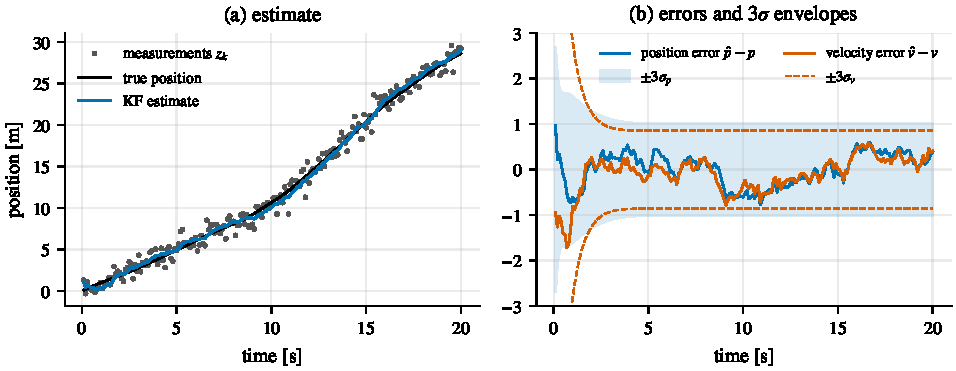
\includegraphics[width=\textwidth]{fig_kf1d.pdf}
  \caption{A constant-velocity Kalman filter tracking a 1D target from noisy position measurements. (a) The estimate smooths the measurements.
  (b) The errors stay inside the $\pm3\sigma$ envelopes, which shrink quickly from the uninformative prior and settle at the steady-state values set by
  the balance between process noise and measurement noise. The velocity is never measured, yet it is estimated through its correlation with
  position.}
  \label{fig:kf1d}
\end{figure}

\Cref{fig:kf1d} shows the filter on the constant-velocity model (\cref{ex:double-integrator-qd}), with position measurements at 10~Hz. Three behaviors
generalize to VIO. The covariance converges from its initial value to a steady state determined only by $Q$, $R$ and the geometry, not by the
data. The unmeasured state (velocity) is estimated through the correlation that the dynamics build up between position and velocity. And the errors
stay inside the $3\sigma$ envelope about 99.7\% of the time, the visual signature of a consistent filter.

\begin{takeaways}
\begin{itemize}
  \item Predict: $\hat x \gets \Phi\hat x$, $P \gets \Phi P\Phi\T + Q$. Update: condition the joint Gaussian of state and measurement.
  \item $K = PH\T S\inv$ maps innovations into state corrections, including corrections to unmeasured but correlated states.
  \item The Kalman filter is the exact Bayesian filter for linear-Gaussian models and the best linear filter otherwise.
  \item Innovations of a correct filter are white with covariance $S$; their NIS is $\chi^2$. This is testable without ground truth.
  \item Time-invariant observable systems reach a steady state set by the balance of process and measurement noise.
  \item Use the Joseph form, solve rather than invert, and symmetrize. Independent measurement blocks may be processed sequentially.
\end{itemize}
\end{takeaways}

\begin{exercises}
  \item Derive \eqref{eq:kf-update} for a scalar state measured twice by independent sensors of variances $R_1$ and $R_2$, first sequentially, then as a
        stacked 2D measurement. Show that the results agree.
  \item Show that $P^+ \preceq P^-$ for the optimal gain. Is this still true for an arbitrary gain in the Joseph form?
  \item Construct a $2\times2$ example in which $(I - KH)P^-$ computed in single precision is not positive semi-definite while the Joseph form is.
  \item Continue the worked example for five more steps and verify that $P_k^-$ converges to 2.
  \item For the scalar random walk with process variance $q$ and measurement variance $r$, derive $P^-_\infty = \tfrac12(q + \sqrt{q^2 + 4qr})$ and the
        steady-state gain. What happens as $q/r \to 0$ and $q/r \to \infty$?
  \item Implement \cref{alg:kf-update} in Python, reproduce \cref{fig:kf1d}, and compute the fraction of time steps where the position error lies outside
        $\pm3\sigma$.
  \item Test the whiteness of the innovations of your filter by computing their sample autocorrelation. Then mis-tune $Q$ and repeat.
\end{exercises}

\chapter{Nonlinear Filtering}
\label{ch:nonlinear}

\begin{objectives}
\begin{itemize}
  \item Derive the extended Kalman filter by linearization, and identify every approximation it makes.
  \item Understand the iterated EKF as Gauss--Newton.
  \item Understand the unscented transform and the unscented Kalman filter.
  \item Understand particle filters and why they do not scale to VIO.
  \item Know why VIO filters are EKFs, and what that implies for how they must be designed.
\end{itemize}
\end{objectives}

Real systems are nonlinear: rotations enter through trigonometric functions, projections divide by depth. A Gaussian pushed through a
nonlinear function is no longer Gaussian (\cref{sec:linearization}), so the exact Bayes filter of \cref{ch:kf} no longer has a finite-dimensional
form. This chapter presents the three main families of approximations. The extended Kalman filter, the basis of this project, is treated in
detail; the others are presented so that the choice is understood.

% ==============================================================================
\section{The extended Kalman filter}

\subsection{The model}

A nonlinear discrete-time model reads
\begin{equation}
  x_k = f(x_{k-1}, u_k, w_k), \qquad z_k = h(x_k) + n_k,
  \label{eq:nonlinear-model}
\end{equation}
with known input $u_k$ (an IMU reading, for instance), process noise $w_k \sim \N(0, Q_k)$ and measurement noise $n_k \sim \N(0, R_k)$.

\subsection{Derivation}

The \term{extended Kalman filter} (EKF) applies the Kalman filter to a linearization of the model about the current estimate.

\paragraph{Prediction.} Expand $f$ to first order around the previous estimate and zero noise:
\begin{equation}
  x_k \approx f(\hat x_{k-1}^+, u_k, 0) + F_k\,(x_{k-1} - \hat x_{k-1}^+) + L_kw_k,
  \qquad F_k = \frac{\partial f}{\partial x}\Big|_{\hat x_{k-1}^+},\quad L_k = \frac{\partial f}{\partial w}\Big|_{\hat x_{k-1}^+} .
\end{equation}
Taking the mean and covariance of the right-hand side (\cref{prop:affine}):
\begin{equation}
  \hat x_k^- = f(\hat x_{k-1}^+, u_k, 0), \qquad P_k^- = F_kP_{k-1}^+F_k\T + L_kQ_kL_k\T .
\end{equation}
The mean is propagated through the \emph{nonlinear} function, the covariance through its Jacobian.

\paragraph{Update.} Expand $h$ around the prediction, $h(x_k) \approx h(\hat x_k^-) + H_k(x_k - \hat x_k^-)$ with $H_k = \partial h/\partial x|_{\hat x_k^-}$, and apply the linear update with
the innovation computed from the nonlinear prediction:
\begin{equation}
\begin{gathered}
  r_k = z_k - h(\hat x_k^-), \qquad S_k = H_kP_k^-H_k\T + R_k, \qquad K_k = P_k^-H_k\T S_k\inv, \\
  \hat x_k^+ = \hat x_k^- + K_kr_k, \qquad P_k^+ = (I - K_kH_k)P_k^-(I - K_kH_k)\T + K_kR_kK_k\T .
\end{gathered}
\end{equation}

\subsection{What the EKF gets wrong}

Every step above is exact for linear models. For nonlinear models the EKF makes three approximations:
\begin{enumerate}
  \item \emph{Gaussianity}: the true prior and posterior are not Gaussian, but are represented by a mean and a covariance.
  \item \emph{Mean bias}: the predicted mean is $f(\hat x)$, not $\E[f(x)]$. By \cref{sec:linearization} the difference is about
        $\tfrac12\sum_ie_i\tr(\nabla^2f_i\,P)$, proportional to the curvature times the covariance.
  \item \emph{Covariance error}: $FPF\T$ ignores higher-order terms, and the Jacobians are evaluated at the \emph{estimate}, not at the unknown true state.
\end{enumerate}
All three errors grow with the size of the uncertainty relative to the scale over which the functions curve. When errors are small, the EKF is
excellent; when they are large, it can be badly wrong, and in particular it can become \emph{inconsistent}: report a covariance smaller than its
actual errors. The third approximation has a subtle long-term consequence in VIO, a spurious gain of information about unobservable directions
(\cref{ch:observability}).

\subsection{The iterated EKF}

By \cref{prop:ekf-gn}, the EKF update is one Gauss--Newton step on the MAP cost $\tfrac12\|x - \hat x^-\|^2_{(P^-)\inv} + \tfrac12\|z - h(x)\|^2_{R\inv}$, linearized at the prior
mean. When the measurement function is strongly nonlinear, that single step can be inaccurate. The \term{iterated EKF} (IEKF) repeats it,
re-linearizing at the latest iterate $x^{(i)}$ while keeping the prior term:
\begin{equation}
  x^{(i+1)} = \hat x^- + K^{(i)}\big(z - h(x^{(i)}) - H^{(i)}(\hat x^- - x^{(i)})\big), \qquad K^{(i)} = P^-H^{(i)\T}\big(H^{(i)}P^-H^{(i)\T} + R\big)\inv,
\end{equation}
with $H^{(i)}$ evaluated at $x^{(i)}$ and $x^{(0)} = \hat x^-$. The first iteration is the EKF. The covariance is computed with the last Jacobian. Iteration
helps when the measurement is very informative relative to the prior, so that the posterior lies far from the prior mean, where the first
linearization is poor.

% ==============================================================================
\section{Sigma-point filters}

\subsection{The unscented transform}

Linearization approximates the \emph{function}. The \term{unscented transform} approximates the \emph{distribution} instead, by a small set of
deterministically chosen \emph{sigma points} that have the right mean and covariance, and pushes each point through the exact nonlinear function.

For $x \in \R^n$ with mean $\mu$ and covariance $P = LL\T$ (Cholesky), choose $\lambda = \alpha^2(n + \kappa) - n$ and the $2n + 1$ points
\begin{equation}
  \chi_0 = \mu, \qquad \chi_i = \mu + \sqrt{n + \lambda}\,\ell_i, \qquad \chi_{n+i} = \mu - \sqrt{n + \lambda}\,\ell_i, \qquad i = 1, \dots, n,
\end{equation}
where $\ell_i$ is the $i$-th column of $L$, with weights
\begin{equation}
  W_0^{(m)} = \frac{\lambda}{n + \lambda}, \quad W_0^{(c)} = \frac{\lambda}{n + \lambda} + (1 - \alpha^2 + \beta), \quad W_i^{(m)} = W_i^{(c)} = \frac{1}{2(n + \lambda)} .
\end{equation}
Propagate $\gamma_i = f(\chi_i)$ and recombine:
\begin{equation}
  \bar y = \sum_iW_i^{(m)}\gamma_i, \qquad P_y = \sum_iW_i^{(c)}(\gamma_i - \bar y)(\gamma_i - \bar y)\T .
\end{equation}
The points are placed symmetrically along the principal axes of the uncertainty, so the weighted points reproduce $\mu$ and $P$ exactly. Expanding $f$
in a Taylor series about $\mu$ shows that $\bar y$ captures the second-order (curvature) term of the mean that linearization misses, and that
$P_y$ is correct to second order, without computing any derivatives. The parameters $\alpha$, $\beta$, $\kappa$ control the spread of the points
($\beta = 2$ is optimal for Gaussians).

\begin{figure}[t]
  \centering
  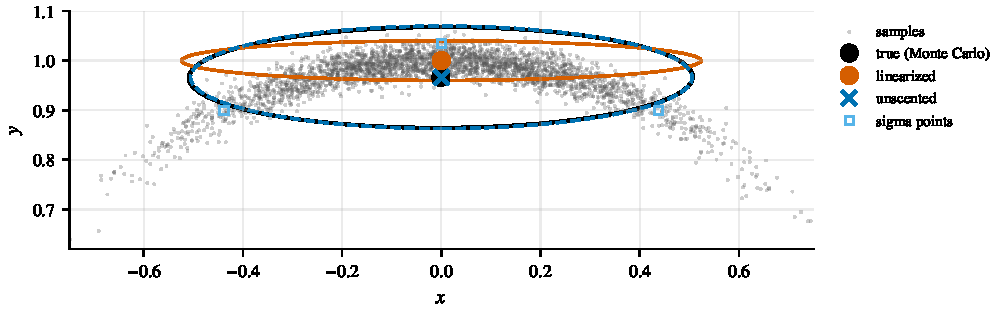
\includegraphics[width=\textwidth]{fig_ut.pdf}
  \caption{A range-bearing measurement converted to Cartesian coordinates, with $\sigma_r = 0.02$ and $\sigma_\phi = 15^\circ$. Monte Carlo samples of the true
  distribution (dots), its true mean and covariance (black), the linearized approximation (orange), and the unscented transform (blue, dashed), with the five
  sigma points; ellipses are $2\sigma$. Linearization places the mean on the circle, where it should not be; the unscented transform recovers the inward shift of the
  mean and a better covariance.}
  \label{fig:ut}
\end{figure}

\subsection{The unscented Kalman filter}

The \emph{unscented Kalman filter} (UKF) uses the unscented transform for both steps. Prediction: generate sigma points from $(\hat x^+, P^+)$, propagate them
through $f$, and recombine into $(\hat x^-, P^-)$, adding $Q$. Update: generate sigma points from $(\hat x^-, P^-)$, push them through $h$ to get the predicted
measurement $\bar z$ and its covariance $S$ (adding $R$), and the cross-covariance $P_{xz} = \sum_iW_i^{(c)}(\chi_i - \hat x^-)(\gamma_i - \bar z)\T$; then
$K = P_{xz}S\inv$, $\hat x^+ = \hat x^- + K(z - \bar z)$ and $P^+ = P^- - KSK\T$. These are the LMMSE formulas of \cref{thm:lmmse} with moments estimated by the
sigma points rather than by linearization. On manifolds, sigma points are generated in the tangent space and mapped with $\bplus$, and their mean is
computed iteratively as in \cref{ch:lie}.

The UKF costs about $2n + 1$ evaluations of $f$ and $h$ per step instead of Jacobians, which is attractive when Jacobians are hard to derive. For VIO
with a 75-dimensional state, the $151$ propagations of the full state per IMU sample are expensive, and the accuracy gain over a well-designed
error-state EKF is small, because the error-state formulation already keeps the nonlinearity mild.

% ==============================================================================
\section{Particle filters}

A \term{particle filter} represents the posterior by $N$ weighted samples (particles) $\{x^{(j)}, w^{(j)}\}$, which can represent any distribution,
multi-modal ones included. The basic \emph{sequential importance resampling} (SIR) algorithm:
\begin{enumerate}
  \item \emph{Predict}: move each particle through the dynamics with a random noise sample, $x_k^{(j)} = f(x_{k-1}^{(j)}, u_k, w^{(j)})$.
  \item \emph{Weight}: multiply each weight by the likelihood of the measurement, $w^{(j)} \gets w^{(j)}p(z_k\mid x_k^{(j)})$, and normalize.
  \item \emph{Resample}: when the effective sample size $N_{\mathrm{eff}} = 1/\sum_j(w^{(j)})^2$ falls too low, draw $N$ new particles with probabilities $w^{(j)}$ and
        reset the weights to $1/N$, so that particles concentrate where the posterior mass is.
\end{enumerate}
Particle filters are exact as $N\to\infty$ and excel at low-dimensional problems with multi-modal posteriors, such as localizing a robot in a known
map. Their weakness is dimension: the number of particles needed to cover a distribution grows roughly exponentially with the state dimension.
For the 15 to 75 dimensions of VIO they are impractical, except in hybrid forms that sample only a few variables.

% ==============================================================================
\section{Why VIO uses the EKF}

\begin{center}\small
\begin{tabularx}{\textwidth}{@{}>{\raggedright\arraybackslash}p{0.2\textwidth}>{\raggedright\arraybackslash}X>{\raggedright\arraybackslash}X>{\raggedright\arraybackslash}X@{}}
\toprule
 & EKF & UKF & particle filter \\
\midrule
cost per step & Jacobians, $\mathcal{O}(n^3)$ & $2n + 1$ propagations, $\mathcal{O}(n^3)$ & $N$ propagations, $N$ huge for large $n$ \\
derivatives needed & yes & no & no \\
non-Gaussian posteriors & no & no & yes \\
accuracy for small errors & excellent & excellent & good (noisy) \\
used in VIO & MSCKF, OpenVINS, ROVIO (iterated) & rarely & no \\
\bottomrule
\end{tabularx}
\end{center}

Visual-inertial odometry has a high-dimensional state, a fast prediction rate (hundreds of Hz), and uncertainties that, once the filter is initialized,
are small compared with the curvature of its models. Those are exactly the conditions under which the EKF is accurate and the alternatives are
expensive. The design principle that makes this work is to keep the linearized errors small: estimate the \emph{error} of a nominal state that
absorbs the large nonlinear motion, and reset it after every correction. That is the error-state Kalman filter of the next chapter.

\begin{takeaways}
\begin{itemize}
  \item The EKF propagates the mean through the nonlinear model and the covariance through its Jacobians, evaluated at the estimate.
  \item Its errors (non-Gaussianity, mean bias, covariance error, estimate-dependent Jacobians) grow with uncertainty relative to curvature.
  \item The iterated EKF is Gauss--Newton on the MAP cost; it helps when measurements are very informative.
  \item The unscented transform propagates sigma points through the exact function and captures second-order effects without derivatives.
  \item Particle filters handle any distribution but scale exponentially with dimension.
  \item VIO uses EKFs with small, frequently reset errors: the error-state formulation.
\end{itemize}
\end{takeaways}

\begin{exercises}
  \item Write the EKF for a planar robot with state $(x, y, \psi)$ driven by speed and turn rate and measured by range to a known beacon. Identify where
        linearization error enters.
  \item Reproduce \cref{fig:ut}. Increase $\sigma_\phi$ until the linearized mean lies outside the $1\sigma$ ellipse of the true distribution.
  \item Show that the unscented transform reproduces the mean and covariance exactly for a linear function.
  \item Show that for a scalar $x \sim \N(\mu, \sigma^2)$ and $f(x) = x^2$, the unscented transform with $n = 1$, $\kappa = 2$, $\alpha = 1$ gives the exact mean $\mu^2 + \sigma^2$.
  \item Implement a particle filter for a 1D robot localizing itself from range measurements to two landmarks, and observe a bimodal posterior.
\end{exercises}
% Solutions to the exercises of Chapter 13.
\begin{solutions}
  \item State $x = (p_x, p_y, \psi)$, inputs $(v, \omega)$ with noise $(n_v, n_\omega)$, beacon at $b = (b_x, b_y)$ with known position.
        \begin{itemize}[leftmargin=1.2em]
          \item \emph{Prediction}: $f(x) = \big(p_x + v\Dt\cos\psi,\ p_y + v\Dt\sin\psi,\ \psi + \omega\Dt\big)$, with Jacobians
                \[
                  F = \begin{bmatrix}1 & 0 & -v\Dt\sin\hat\psi\\ 0 & 1 & v\Dt\cos\hat\psi\\ 0 & 0 & 1\end{bmatrix}, \qquad
                  L = \begin{bmatrix}\Dt\cos\hat\psi & 0\\ \Dt\sin\hat\psi & 0\\ 0 & \Dt\end{bmatrix},
                \]
                and $P^- = FPF\T + L\diag(\sigma_v^2, \sigma_\omega^2)L\T$.
          \item \emph{Update}: $h(x) = \rho = \|p - b\|$, $H = \big[(\hat p_x - b_x)/\hat\rho,\ (\hat p_y - b_y)/\hat\rho,\ 0\big]$, then the standard update.
        \end{itemize}
        Linearization error enters in three places. (i) In the prediction through $\cos\psi$ and $\sin\psi$: with a large heading uncertainty the predicted
        positions spread along an arc, the banana of \cref{fig:banana}, which $FPF\T$ approximates by an ellipse. (ii) In the update through the curvature of the
        range: $\nabla^2h$ has the eigenvalue $1/\rho$ in the direction perpendicular to the line of sight, so the neglected second-order term is about
        $\sigma_\perp^2/(2\rho)$, harmless far from the beacon and large close to it (and $H$ is undefined at $\rho = 0$). (iii) In the heading: the range does not
        depend on $\psi$ ($H_\psi = 0$), so the heading is corrected only through the position-heading correlation that motion builds in $P$, which is
        itself a linearized quantity. When the heading error is large, those correlations are wrong and the corrections are too.

  \item With the figure's $\sigma_r = 0.02$, the true distribution of $(x, y) = (r\cos\phi, r\sin\phi)$ for $\phi \sim \N(\pi/2, \sigma_\phi^2)$ has mean $(0, e^{-\sigma_\phi^2/2})$ and
        $\Var(y) = (1 + \sigma_r^2)(1 + e^{-2\sigma_\phi^2})/2 - e^{-\sigma_\phi^2}$, while linearization predicts the mean $(0, 1)$. The covariance is diagonal by symmetry,
        so the Mahalanobis distance of the linearized mean is $d = (1 - e^{-\sigma_\phi^2/2})/\sqrt{\Var(y)}$:
        \begin{center}\small
        \begin{tabular}{@{}l c c c c c c@{}}
        \toprule
        $\sigma_\phi$ & $15^\circ$ & $30^\circ$ & $45^\circ$ & $60^\circ$ & $75^\circ$ & $90^\circ$ \\
        \midrule
        $d$ & 0.67 & 0.75 & 0.81 & 0.90 & 0.99 & 1.10 \\
        \bottomrule
        \end{tabular}
        \end{center}
        The linearized mean leaves the $1\sigma$ ellipse at $\sigma_\phi \approx 76^\circ$ (confirmed by Monte Carlo). Notice that it never gets very far: in the
        small-angle regime $d^2 \approx (\sigma_\phi^4/4)/(\sigma_r^2 + \sigma_\phi^4/2) < \tfrac12$, because the true distribution spreads along the arc as fast as its mean moves
        inward. The more telling failure is the shape: the true distribution is a thin curved arc, and the linearized ellipse puts most of its
        probability where the true one has none.

  \item For $f(x) = Ax + b$ the transformed sigma points are $y_0 = A\mu + b$ and $y_{i}, y_{n+i} = A\mu + b \pm\sqrt{n + \lambda}\,A\ell_i$. The mean weights sum to
        one ($\frac{\lambda}{n + \lambda} + \frac{2n}{2(n + \lambda)} = 1$) and the $\pm$ pairs cancel, so $\bar y = \sum_iW_i^{(m)}y_i = A\mu + b$. In the covariance the central point
        contributes nothing ($y_0 - \bar y = 0$, so the value of $W_0^{(c)}$ and of $\beta$ is irrelevant), and each pair contributes
        $2\cdot\frac{1}{2(n + \lambda)}(n + \lambda)A\ell_i\ell_i\T A\T$:
        \[
          \sum_iW_i^{(c)}(y_i - \bar y)(y_i - \bar y)\T = A\Big(\sum_{i=1}^n\ell_i\ell_i\T\Big)A\T = ALL\T A\T = APA\T .
        \]
        The unscented transform is exact for linear functions, as it must be to be consistent with the Kalman filter.

  \item With $n = 1$, $\kappa = 2$ and $\alpha = 1$: $\lambda = 1\cdot3 - 1 = 2$, $n + \lambda = 3$, sigma points $\mu$ and $\mu \pm \sqrt3\,\sigma$, weights $W_0^{(m)} = \tfrac23$ and
        $W_{1,2}^{(m)} = \tfrac16$. For $f(x) = x^2$,
        \[
          \tfrac23\mu^2 + \tfrac16\big((\mu + \sqrt3\sigma)^2 + (\mu - \sqrt3\sigma)^2\big) = \tfrac23\mu^2 + \tfrac16\big(2\mu^2 + 6\sigma^2\big) = \mu^2 + \sigma^2 = \E[x^2],
        \]
        exactly, whereas linearization gives $\mu^2$. (The choice $\kappa = 3 - n$ also makes the sigma points reproduce the fourth moment $3\sigma^4$ of a scalar
        Gaussian: $\tfrac16\cdot2\cdot9\sigma^4 = 3\sigma^4$.)

  \item A simple model that produces bimodality: landmarks at $0$ and $10$ on a line, and a sensor that reports the range to the \emph{nearest} landmark
        without saying which one it is ($z = \min(|x|, |x - 10|) + n$, $\sigma_z = 0.1$). The robot starts at $x = 2$ with a uniform prior on $[0, 10]$ and
        then moves right by $0.5$ per step (odometry noise $0.05$). A bootstrap particle filter with 2000 particles: propagate each particle with the
        odometry plus sampled noise, multiply its weight by the likelihood $\exp(-(z - h(x_i))^2/2\sigma_z^2)$, normalize, and resample when the effective
        sample size $1/\sum_iw_i^2$ drops below $N/2$. After the first measurement ($z = 1.87$) the posterior has two equal modes, near $1.9$ and near $8.1$
        (weights $0.52$ and $0.48$), symmetric about $5$; its mean, $4.9$, is a place where the robot certainly is not, which is what a Gaussian filter
        would report. After the first move the mirror hypothesis predicts a range of about $1.4$ (it approaches the landmark at 10) while the
        measurement says $2.3$; its weight drops to zero and the filter tracks the true position from then on. A Kalman-type filter cannot represent
        the bimodal stage at all: it would either lock onto one mode, possibly the wrong one, or average them.
\end{solutions}


\chapter{The Error-State Kalman Filter}
\label{ch:eskf}

\begin{objectives}
\begin{itemize}
  \item Understand the three-way split into true, nominal and error state, and why it is the right way to filter on a manifold.
  \item Derive the linearized error dynamics with a mechanical recipe.
  \item Define measurement residuals and Jacobians on the manifold with the correct sign convention.
  \item Derive the injection and reset steps, including the reset Jacobian $G$.
  \item Assemble the complete error-state Kalman filter loop, and follow it through a complete attitude-estimation example.
\end{itemize}
\end{objectives}

% ==============================================================================
\section{Filtering on a manifold}

The EKF of \cref{ch:nonlinear} assumes the state lives in $\R^n$, so that $\hat x + Kr$ makes sense. For VIO, the state contains a rotation, which does
not live in a vector space (\cref{ch:lie}). Three quantities must therefore be distinguished.

\begin{definition}[True, nominal and error state]
\index{error state}\index{nominal state}
\begin{itemize}
  \item The \textbf{true state} $x$ is the unknown physical state, a point on the state manifold $\mathcal{M}$.
  \item The \textbf{nominal state} $\hat x \in \mathcal{M}$ is the current best estimate, propagated with the full nonlinear model and no noise.
  \item The \textbf{error state} $\delta x = x \bminus \hat x \in \R^{n}$ is the small, minimal-dimension difference, defined with the operators of
        \cref{sec:boxplus}.
\end{itemize}
The filter's Gaussian belief is over the error state: $\delta x \sim \N(\delta\hat x, P)$, so that $x = \hat x \bplus \delta x$.
\end{definition}

For the IMU state this means 16 nominal numbers (quaternion included) but a 15-dimensional error and a $15\times15$ covariance, with no redundant
directions and no constraints. The Kalman filter operates only on the error state, which is a vector, so all of \cref{ch:kf} applies to it. This
design is called the \term{error-state Kalman filter} (ESKF), or \emph{indirect} Kalman filter. In aerospace the same idea for attitude is the
\emph{multiplicative} EKF.

\begin{keyidea}[why the error state]
\begin{itemize}
  \item \textbf{Minimal and unconstrained.} The error has exactly as many components as degrees of freedom, so its covariance is non-singular and
        needs no constraint handling.
  \item \textbf{Always near the origin.} After every update the error is reset to zero, so it never approaches the singularities of
        three-parameter rotations, and the small-angle approximations used to derive its dynamics remain valid.
  \item \textbf{Nearly linear.} The large, fast, nonlinear motion is carried by the nominal state, which is integrated exactly. The error evolves
        slowly and is small, so its dynamics are almost linear and linearization is accurate (\cref{ch:nonlinear}).
  \item \textbf{Slow.} Error dynamics are governed by sensor errors, not by vehicle motion, so the covariance could even be propagated at a lower rate
        than the nominal state if computation were scarce.
\end{itemize}
\end{keyidea}

% ==============================================================================
\section{The ESKF cycle}

\begin{figure}[t]
\centering
\begin{tikzpicture}[node distance=14mm and 30mm]
  \node[block, minimum width=40mm] (nom) {\textbf{1. Nominal propagation}\\ $\hat x \gets f(\hat x, u)$, noise-free, nonlinear};
  \node[block, minimum width=40mm, right=of nom] (cov) {\textbf{2. Covariance propagation}\\ $P \gets \Phi P\Phi\T + Q_d$};
  \node[block, minimum width=40mm, below=of cov] (upd) {\textbf{3. Update}\\ $r = z\bminus h(\hat x)$, \ $\delta\hat x = Kr$\\ $P \gets$ Joseph form};
  \node[block, minimum width=40mm, below=of nom] (inj) {\textbf{4. Inject and reset}\\ $\hat x \gets \hat x\bplus\delta\hat x$, \ $\delta\hat x \gets 0$\\ $P \gets GPG\T$};
  \draw[->, thick] (nom) -- node[note, above]{every IMU} node[note, below]{sample} (cov);
  \draw[->, thick] (cov) -- node[note, right, align=left]{measurement\\arrives} (upd);
  \draw[->, thick] (upd) -- (inj);
  \draw[->, thick] (inj) -- (nom);
  \draw[->, thick, dashed] (cov.north) to[out=135, in=45] node[note, above]{no measurement: next IMU sample} (nom.north);
\end{tikzpicture}
\caption{The error-state Kalman filter cycle. The error-state mean is zero throughout propagation, so only the covariance is propagated in step 2. It
becomes non-zero in step 3 and is transferred to the nominal state and zeroed in step 4.}
\label{fig:eskf-cycle}
\end{figure}

\Cref{fig:eskf-cycle} shows the four steps.
\begin{enumerate}
  \item \textbf{Nominal propagation.} At each IMU sample, integrate the nonlinear kinematics with the measured inputs, ignoring noise
        (\cref{ch:strapdown}).
  \item \textbf{Error covariance propagation.} Propagate $P$ with the linearized error dynamics (\cref{ch:errordyn}).
  \item \textbf{Update.} When a measurement arrives, compute the residual and its Jacobian on the manifold, and compute the Kalman estimate of the
        error, $\delta\hat x = Kr$, and the posterior covariance.
  \item \textbf{Injection and reset.} Move the estimated error into the nominal state with $\bplus$, set the error mean back to zero, and correct the
        covariance for the change of reference point.
\end{enumerate}

\begin{proposition}[The error mean needs no propagation]
If $\delta\hat x = 0$ after a reset, and the error obeys linear dynamics $\dot{\delta x} = F_c\delta x + G_cw$ with zero-mean noise, then $\E[\delta x] = 0$ until the
next update.
\end{proposition}
\begin{proof}
The mean obeys $\frac{\dd}{\dd t}\E[\delta x] = F_c\,\E[\delta x]$ (\cref{prop:lyapunov}) with initial value zero, whose unique solution is zero.
\end{proof}

This is why step 2 propagates only the covariance: all the knowledge of the error state's mean has been transferred into the nominal state.

% ==============================================================================
\section{Linearized error dynamics: the recipe}
\label{sec:error-dyn-recipe}

Suppose the true state obeys $\dot x = f(x, u, w)$ with noise $w$, and the nominal state obeys $\dot{\hat x} = f(\hat x, u, 0)$. The error dynamics are
derived in four mechanical steps.
\begin{enumerate}
  \item Write the true dynamics block by block.
  \item Substitute $x = \hat x\bplus\delta x$ in every block. For the attitude, $R = \hat R\Exp(\delta\theta)$ (or $\Exp(\delta\theta)\hat R$ for a global perturbation).
  \item Subtract the nominal dynamics.
  \item Keep only terms of first order in the small quantities ($\delta x$ and $w$), using $\Exp(\delta\theta) \approx I + \sx{\delta\theta}$ and dropping their
        products.
\end{enumerate}
The result is a linear time-varying system
\begin{equation}
  \dot{\delta x} = F_c(\hat x, u)\,\delta x + G_c(\hat x)\,w,
\end{equation}
which \cref{sec:discretization} turns into $\Phi$ and $Q_d$. The attitude block needs the time derivative of the perturbation itself, worked out in
\cref{lem:dexp}. \Cref{sec:ahrs} applies the recipe to a complete small filter, and \cref{ch:errordyn} to the inertial navigation equations.

% ==============================================================================
\section{Measurement updates on the manifold}
\label{sec:manifold-update}

Let a sensor produce a measurement $z$ on a manifold $\mathcal{Z}$ (a vector space, $\SO$, a pose, \dots) according to the generative model
\begin{equation}
  z = h(x)\bplus n, \qquad n \sim \N(0, R_z).
\end{equation}
The ESKF compares the measurement with its prediction from the nominal state,
\begin{equation}
  r = z \bminus h(\hat x),
  \label{eq:manifold-residual}
\end{equation}
and models how the residual depends on the unknown true error $\delta x$. Substituting $z = h(\hat x\bplus\delta x)\bplus n$ and linearizing,
\begin{equation}
  r \approx H\,\delta x + n, \qquad
  H = \frac{\partial}{\partial\delta x}\Big[ h(\hat x\bplus\delta x)\bminus h(\hat x) \Big]_{\delta x = 0}.
  \label{eq:manifold-H}
\end{equation}
$H$ is the manifold Jacobian of $h$ (\cref{def:manifold-jacobian}). With $r$ and $H$, the update is the ordinary Kalman update of the error state
with prior $\N(0, P)$:
\begin{equation}
  S = HPH\T + R_z,\qquad K = PH\T S\inv,\qquad \delta\hat x = Kr,\qquad P^+ = (I - KH)P(I - KH)\T + KR_zK\T.
\end{equation}

\begin{pitfall}[the sign of $H$]
There are two ways to set up the linearization, and they differ by a sign. The generative view above differentiates the \emph{prediction} with
respect to the \emph{true} error: $r \approx +H\delta x$. An optimization view instead writes the residual as a function of a correction $\delta$ to the
estimate, $e(\delta) = z\bminus h(\hat x\bplus\delta)$, whose Jacobian is $-H$ (to first order). Both lead to the same correction if used consistently.
Mixing them flips every correction. In this project, $H$ is always \eqref{eq:manifold-H}, and its finite-difference test perturbs the nominal state:
$r(\delta x) := h(\hat x\bplus\delta x)\bminus h(\hat x)$ and $H \approx \partial r/\partial\delta x$.
\end{pitfall}

For a vector-valued measurement, $\bminus$ is subtraction and this reduces to the EKF. For a rotation-valued measurement such as the pose
measurement of Milestone 6, the attitude part of the residual is $\Log_q(\hat q\inv\qprod q_{meas})$ (AGENTS.md F3).

% ==============================================================================
\section{Injection and reset}
\label{sec:reset}

After the update, the error estimate $\delta\hat x = Kr$ is non-zero. Injection moves it into the nominal state:
\begin{equation}
  \hat x^+ = \hat x\bplus\delta\hat x:\quad
  \hat p \gets \hat p + \delta\hat p,\quad \hat v \gets \hat v + \delta\hat v,\quad
  \hat q \gets \hat q\qprod\Exp_q(\delta\hat\theta),\quad \hat b \gets \hat b + \delta\hat b,
\end{equation}
followed by normalization of every quaternion that was touched, for the IMU and every clone (AGENTS.md F4).

The error is now defined relative to the new nominal state, $\delta x^+ = x\bminus\hat x^+$, and its mean is zero. But its covariance is not exactly $P^+$,
because the reference point of the tangent space has moved.

\begin{proposition}[Reset Jacobian]
\label{prop:reset}
\index{reset Jacobian}
Let $\delta x \sim \N(\delta\hat x, P^+)$ be the error relative to $\hat x$ after the update, and $\delta x^+ = x\bminus(\hat x\bplus\delta\hat x)$ the error relative to the
injected nominal state. To first order, $\delta x^+ \sim \N(0, GP^+G\T)$ with $G = \partial\delta x^+/\partial\delta x$ evaluated at $\delta\hat x$. For the vector blocks
$G = I$, and for each attitude block
\begin{equation}
  G_\theta = I - \tfrac12\sx{\delta\hat\theta}.
  \label{eq:reset-G}
\end{equation}
\end{proposition}
\begin{proof}
For vector blocks $\delta x^+ = \delta x - \delta\hat x$, whose Jacobian is $I$. For the attitude, $q = \hat q\qprod\Exp_q(\delta\theta)$ and
$q = \hat q^+\qprod\Exp_q(\delta\theta^+)$ with $\hat q^+ = \hat q\qprod\Exp_q(\delta\hat\theta)$, so
\begin{equation*}
  \Exp(\delta\theta^+) = \Exp(-\delta\hat\theta)\,\Exp(\delta\theta).
\end{equation*}
By the BCH formula \eqref{eq:bch}, $\delta\theta^+ = \delta\theta - \delta\hat\theta - \tfrac12\,\delta\hat\theta\times\delta\theta + \cdots$, whose derivative with respect to $\delta\theta$ is
$I - \tfrac12\sx{\delta\hat\theta}$. At $\delta\theta = \delta\hat\theta$ the value is exactly zero, so the new error has zero mean. Linearizing $\delta x^+$ about $\delta\hat x$ and applying
\cref{prop:affine} gives the covariance.
\end{proof}

\begin{remark}[relation to the right Jacobian]
The derivative of $\Log(\Exp(-\delta\hat\theta)\Exp(\delta\theta))$ at $\delta\theta = \delta\hat\theta$ can be computed exactly with \eqref{eq:jr-def}: it is
$\Jr(\delta\hat\theta) = I - \tfrac12\sx{\delta\hat\theta} + O(\|\delta\hat\theta\|^2)$. The frozen specification (AGENTS.md F4) uses the first-order form \eqref{eq:reset-G}. For a
typical correction of a few milliradians the two differ by about $10^{-6}$ and the difference is irrelevant. Changing it would be a logged
convention change, not a silent substitution.
\end{remark}

The covariance reset is therefore
\begin{equation}
  P \gets G P G\T, \qquad G = \blkdiag\big(I_6,\ I - \tfrac12\sx{\delta\hat\theta},\ I_6,\ \ldots\big),
\end{equation}
with one $I - \tfrac12\sx{\delta\hat\theta_i}$ block for each clone's attitude and identity elsewhere.

\begin{convention}[injection and reset, AGENTS.md F4]
Inject with $\bplus$ into the IMU block and every clone; normalize every touched quaternion; reset $\delta\hat x \gets 0$ and $P \gets GPG\T$ with $G$
implemented exactly as above. Using $G \approx I$ is a deviation that must be logged.
\end{convention}

How much does $G$ matter? It rotates the attitude covariance by half the injected correction, a first-order effect in $\|\delta\hat\theta\|$. With small
corrections at high rate the effect is tiny, and many implementations use $G = I$. Large corrections (after a long outage, or a loop closure) make it
noticeable. It costs almost nothing, and implementing it exactly removes one approximation from the consistency analysis of Milestone 7.

% ==============================================================================
\section{The complete error-state filter}

\begin{algorithm}[t]
\caption{Error-state Kalman filter (one IMU step and an optional update)}
\label{alg:eskf}
\begin{algorithmic}[1]
\Require nominal $\hat x$, covariance $P$, IMU sample at $t_k$, optional measurement $z$ at $t_k$
\State $\Dt \gets t_k - t_{k-1}$ \Comment{from integer nanosecond timestamps}
\State $\hat x \gets f(\hat x, u_k, \Dt)$; normalize $\hat q$ \Comment{nominal propagation}
\State $\Phi \gets I + F_c\Dt$; \quad $Q_d \gets G_cQ_cG_c\T\Dt$
\State $P \gets \Phi P\Phi\T + Q_d$; \quad $P \gets \tfrac12(P + P\T)$
\If{measurement $z$ available}
  \State $r \gets z\bminus h(\hat x)$; \quad $H \gets \partial[h(\hat x\bplus\delta x)\bminus h(\hat x)]/\partial\delta x$
  \State $S \gets HPH\T + R_z$; factor $S$; gate on $r\T S\inv r$
  \State $K \gets PH\T S\inv$ (by solving); \quad $\delta\hat x \gets Kr$
  \State $P \gets (I-KH)P(I-KH)\T + KR_zK\T$
  \State $\hat x \gets \hat x\bplus\delta\hat x$; normalize quaternions \Comment{inject}
  \State $P \gets GPG\T$; \quad $P \gets \tfrac12(P + P\T)$ \Comment{reset}
\EndIf
\end{algorithmic}
\end{algorithm}

\Cref{alg:eskf} assembles the pieces. It is generic: \cref{ch:strapdown,ch:errordyn} supply $f$, $F_c$ and $G_c$ for the IMU, \cref{ch:updates} supplies $h$ and $H$ for a
pose sensor, and \cref{ch:msckfupdate} supplies them for a camera. When measurements arrive between IMU samples, the filter first propagates to the
measurement time by splitting the IMU interval (\cref{ch:strapdown}).

% ==============================================================================
\section{A complete example: attitude estimation}
\label{sec:ahrs}

\index{attitude estimation}
To see every step of \cref{alg:eskf} at work on a problem small enough to follow completely, consider an \emph{attitude and heading reference system}
(AHRS) without a magnetometer: estimate the attitude $R = R_{wb}$ of a slowly moving device and the bias $b$ of its gyroscope, using the gyroscope for
propagation and the accelerometer as an inclinometer (it measures the reaction to gravity when linear accelerations are small).

To avoid solving the project's own derivation exercise, this example uses the \textbf{global} perturbation $R = \Exp(\delta\theta)\hat R$, with the error
expressed in the world frame. The project's state uses the local perturbation; its forms are the subject of the derivation exercises of \cref{ch:errordyn}\ifsolutions{}
(solutions in \cref{app:solutions})\fi.

\paragraph{State and error state.} Nominal $(\hat R, \hat b)$; error $\delta x = (\delta\theta, \delta b) \in \R^6$ with $R = \Exp(\delta\theta)\hat R$ and $b = \hat b + \delta b$.

\paragraph{Models.} Gyroscope $\omega_m = \omega + b + n_g$; bias random walk $\dot b = n_b$; accelerometer at rest $a_m = R\T v + n_a$ with $v = -g_w = (0, 0, 9.81)$.

\paragraph{Nominal propagation.} $\hat R \gets \hat R\Exp\big((\omega_m - \hat b)\Dt\big)$, $\hat b$ unchanged.

\paragraph{Error dynamics.} By \cref{ex:global-attitude} (in \cref{ch:errordyn}), $\dot{\delta\theta} = -\hat R\,\delta b - \hat R\,n_g$, and $\dot{\delta b} = n_b$. Hence
\begin{equation}
  F_c = \begin{bmatrix} 0 & -\hat R \\ 0 & 0\end{bmatrix}, \qquad G_c = \begin{bmatrix} -\hat R & 0 \\ 0 & I\end{bmatrix}, \qquad Q_c = \diag(\sigma_g^2I, \sigma_b^2I).
\end{equation}

\paragraph{Measurement Jacobian.} $h(x) = R\T v$. Perturbing, $h(\Exp(\delta\theta)\hat R) = \hat R\T\Exp(-\delta\theta)v \approx \hat R\T(v - \delta\theta\times v) = \hat R\T v + \hat R\T\sx{v}\,\delta\theta$, so
\begin{equation}
  H = \begin{bmatrix} \hat R\T\sx{v} & 0 \end{bmatrix}, \qquad r = a_m - \hat R\T v .
\end{equation}
$\sx{v}$ has rank two: the measurement observes the two components of $\delta\theta$ perpendicular to gravity (roll and pitch) but not the component along it
(yaw). It does not observe the bias directly at all.

\paragraph{Injection and reset.} $\hat R \gets \Exp(\delta\hat\theta)\hat R$, $\hat b \gets \hat b + \delta\hat b$. Repeating the reset derivation for the global perturbation,
$\Exp(\delta\theta^+) = \Exp(\delta\theta)\Exp(-\delta\hat\theta)$, gives $G_\theta = I + \tfrac12\sx{\delta\hat\theta}$: the same magnitude as \eqref{eq:reset-G}, opposite sign.

\begin{figure}[t]
  \centering
  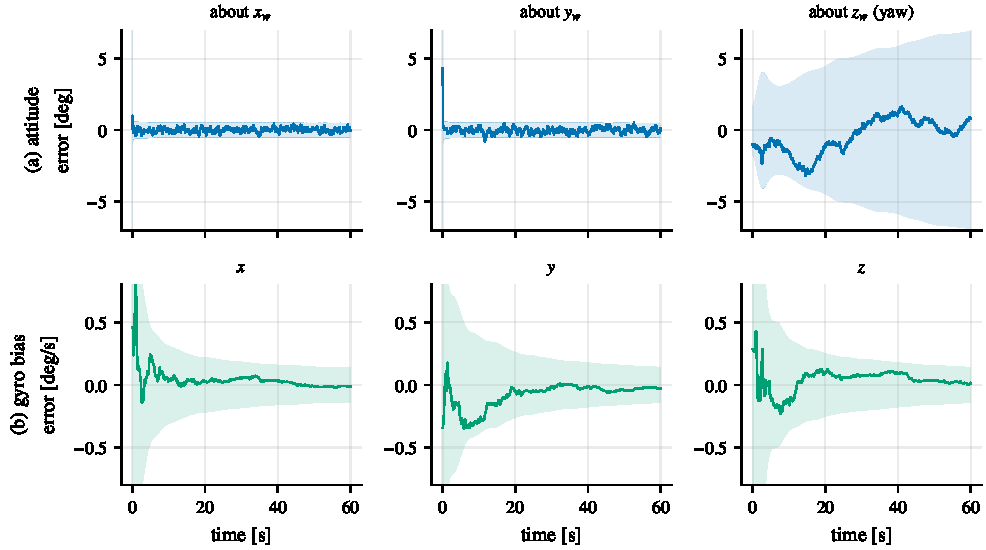
\includegraphics[width=\textwidth]{fig_ahrs.pdf}
  \caption{The attitude ESKF of \cref{sec:ahrs} on a simulated tumbling device: gyroscope at 100~Hz with a constant bias, accelerometer used as an
  inclinometer at 10~Hz. (a) Attitude errors about the world axes with their $\pm3\sigma$ bounds. Tilt (about $x$ and $y$) is quickly bounded by the
  accelerometer; the error about the vertical (yaw) is unobservable, and its bound grows. (b) Gyro bias errors with $\pm3\sigma$ bounds. The bias
  is never measured directly, yet all three components converge, because the device's rotation makes each body axis horizontal at some time.}
  \label{fig:ahrs}
\end{figure}

\Cref{fig:ahrs} shows the filter on simulated data. Several lessons of this chapter are visible in it. The errors stay inside their $3\sigma$
bounds: the filter is consistent. Tilt becomes accurate within seconds, through the accelerometer. Yaw is unobservable without a magnetometer
or vision, so its uncertainty only grows. And the gyro bias, although never measured, is estimated through its correlation with the tilt error
it causes: the cross-covariance built by propagation lets the gain correct it. This is exactly how the full VIO filter estimates IMU biases from
camera measurements.

\begin{projectlink}[Milestones 4--6]
M4 implements step 2 of \cref{alg:eskf}, M5 steps 3--4, and M6 the update, injection and reset with a pose measurement. Testing them separately
localizes bugs: if propagation is exact on synthetic data, and the covariance matches Monte Carlo statistics, then any later inconsistency is in
the update.
\end{projectlink}

\begin{takeaways}
\begin{itemize}
  \item The ESKF splits the state into a nonlinear nominal part and a small, minimal, nearly linear error part. The Kalman filter only ever sees the
        error.
  \item The error mean is zero during propagation; only $P$ is propagated.
  \item Residual $r = z\bminus h(\hat x) \approx H\delta x + n$ with $H$ the manifold Jacobian of $h$ at $\hat x$.
  \item After injection, reset $P \gets GPG\T$ with $G_\theta = I - \tfrac12\sx{\delta\hat\theta}$ for every (local) attitude block.
  \item The attitude example shows observability at work: gravity bounds tilt, yaw drifts, and unmeasured biases are estimated through
        correlations.
\end{itemize}
\end{takeaways}

\begin{exercises}
  \item Derive the reset Jacobian for the global perturbation $R = \Exp(\delta\theta)\hat R$ and confirm $G_\theta = I + \tfrac12\sx{\delta\hat\theta}$.
  \item Suppose $\delta\hat\theta = (0, 0, 0.1)$~rad and $P_{\theta\theta} = \diag(10^{-4}, 10^{-4}, 10^{-2})$. Compute $GP_{\theta\theta}G\T$ and compare with
        $\Jr(\delta\hat\theta)P_{\theta\theta}\Jr(\delta\hat\theta)\T$. When is the difference noticeable?
  \item An iterated ESKF repeats the update with $H$ re-evaluated at $\hat x\bplus\delta\hat x$. Show that one iteration is a Gauss--Newton step on the MAP cost
        $\|\delta x\|^2_{P\inv} + \|z\bminus h(\hat x\bplus\delta x)\|^2_{R_z\inv}$.
  \item Implement the attitude filter of \cref{sec:ahrs} and reproduce \cref{fig:ahrs}. Then hold the device still and observe which bias component stops
        converging. Explain why.
  \item Rewrite the attitude filter with the local perturbation $R = \hat R\Exp(\delta\theta)$: derive $F_c$, $G_c$, $H$ and $G$. (This is a small version of the project's
        derivation exercise.)
\end{exercises}
% Solutions to the exercises of Chapter 14.
\begin{solutions}
  \item With the global perturbation the true attitude is $R = \Exp(\delta\theta)\hat R$ before injection and $R = \Exp(\delta\theta^+)\hat R^+$ after it, with
        $\hat R^+ = \Exp(\delta\hat\theta)\hat R$. Equating, $\Exp(\delta\theta^+) = \Exp(\delta\theta)\Exp(-\delta\hat\theta)$, and the BCH formula \eqref{eq:bch} gives
        \[
          \delta\theta^+ = \delta\theta - \delta\hat\theta - \tfrac12\,\delta\theta\times\delta\hat\theta + \cdots = \delta\theta - \delta\hat\theta + \tfrac12\,\delta\hat\theta\times\delta\theta + \cdots,
        \]
        whose derivative with respect to $\delta\theta$ is $G_\theta = I + \tfrac12\sx{\delta\hat\theta}$. The sign is opposite to the local case
        (\cref{prop:reset}), because the correction now multiplies on the left. (Exactly, the derivative at $\delta\theta = \delta\hat\theta$ is $\Jl(\delta\hat\theta)$.)

  \item Here $\sx{\delta\hat\theta}$ mixes only $x$ and $y$, and $P_{\theta\theta}$ is isotropic in that plane, so both products stay diagonal:
        \begin{align*}
          GP_{\theta\theta}G\T &= \diag\big(1.0025,\ 1.0025,\ 100\big)\times10^{-4}, \\
          \Jr P_{\theta\theta}\Jr\T &= \diag\big(0.9992,\ 0.9992,\ 100\big)\times10^{-4}.
        \end{align*}
        The difference, $0.33\%$ of the $x$ and $y$ variances, is second order: $G$ and $\Jr(\delta\hat\theta) = I - \tfrac12\sx{\delta\hat\theta} + O(\|\delta\hat\theta\|^2)$ agree to
        first order, and their products differ by about $\|\delta\hat\theta\|^2/3$. For anisotropic covariances the first-order rotation of the covariance is the
        same in both, and the relative difference is about $3\times10^{-6}$, $3\times10^{-4}$, $3\%$ and $40\%$ for corrections of $0.003$, $0.03$, $0.3$ and $1$~rad. It
        is negligible for the milliradian corrections of a running filter and noticeable only after very large corrections, such as the first updates
        after a poor initialization.

  \item Let $\delta x$ be the error-state variable with prior $\N(0, P)$ in the tangent space at $\hat x$, and $r(\delta x) = z\bminus h(\hat x\bplus\delta x)$, so that the MAP
        cost is $F(\delta x) = \|\delta x\|^2_{P\inv} + \|r(\delta x)\|^2_{R_z\inv}$. Near an iterate $\delta x_i$, $r(\delta x) \approx r_i - H_i(\delta x - \delta x_i)$ with $r_i = r(\delta x_i)$ and $H_i$ the
        manifold Jacobian of $h$ at $\hat x\bplus\delta x_i$. Minimizing the resulting quadratic gives the Gauss--Newton iterate (the algebra of Exercise 10.7 with
        $\mu = 0$)
        \[
          \delta x_{i+1} = K_i\big(r_i + H_i\,\delta x_i\big), \qquad K_i = PH_i\T\big(H_iPH_i\T + R_z\big)\inv .
        \]
        From $\delta x_0 = 0$ the first iterate is $\delta x_1 = K_0r(0)$ with $H_0$ evaluated at $\hat x$: exactly the ESKF update $\delta\hat x = Kr$. One ESKF update is
        therefore one Gauss--Newton step on the MAP cost; the iterated ESKF re-evaluates $h$ and $H$ at $\hat x\bplus\delta x_i$ and repeats, then injects the final
        $\delta x$ and resets once.

  \item The code of \cref{fig:ahrs} is \code{fig\_ahrs} in \code{scripts/figures\_extra.py}. With the tumbling motion all three bias errors converge,
        ending with standard deviations of about $8\times10^{-4}$~rad/s and errors within them. Holding the device still and level (zero rate) instead, the
        two horizontal components still converge ($\sigma \approx 6.5\times10^{-4}$~rad/s, errors consistent with it), but the vertical component, along the measured
        gravity, does not: its error stays near its initial $0.01$~rad/s. A bias about the vertical integrates into a yaw error, and an inclinometer
        cannot see yaw; to first order that bias is unobservable. Under rotation, every body axis is horizontal at some time, and a bias about a
        horizontal axis produces a tilt that the accelerometer does see. (The filter's own $\sigma$ for the vertical component nevertheless shrinks to about
        $0.004$~rad/s, so its error sits near $2.7\sigma$. With the bias unobservable the yaw estimate drifts far from the truth, $0.3$~rad in a minute, and
        Jacobians evaluated at that drifting estimate inject information the data do not contain. Evaluated at the true attitude, the same filter's
        error is consistent with its $\sigma$. This is a first encounter with the mechanism analyzed in \cref{ch:observability}.)

  \item \ifsolutions
        With $R = \hat R\Exp(\delta\theta)$, $\hat\omega = \omega_m - \hat b$ and $\omega = \omega_m - b - n_g = \hat\omega - \delta b - n_g$, \cref{lem:dexp} applied to
        $\dot R = R\sx{\omega}$ gives, to first order, $\dot{\delta\theta} = -\sx{\hat\omega}\delta\theta - \delta b - n_g$; and $\dot{\delta b} = n_b$. Hence
        \[
          F_c = \begin{bmatrix}-\sx{\hat\omega} & -I\\ 0 & 0\end{bmatrix}, \qquad G_c = \begin{bmatrix}-I & 0\\ 0 & I\end{bmatrix}.
        \]
        For the inclinometer, $h = R\T v$, and the inverse-action row of \cref{tab:jacobians} gives
        \[
          h(\hat R\Exp(\delta\theta)) \approx \hat R\T v + \sx{\hat R\T v}\,\delta\theta, \qquad\text{so}\qquad H = \big[\sx{\hat R\T v}\ \ 0\big].
        \] The reset is $G = \blkdiag\big(I - \tfrac12\sx{\delta\hat\theta},\ I\big)$ (\cref{prop:reset}). Compared with the global version of
        \cref{sec:ahrs}, the heading-dependent $\hat R$ has disappeared from $F_c$ and $G_c$ and moved into $H$, and the error is coupled to the rotation through
        $-\sx{\hat\omega}$: a body-frame error appears to rotate backwards as the body turns. These are exactly the attitude rows of the project's $F_c$ and $G_c$.
        \else\withheldsolution\fi
\end{solutions}



\part{Inertial Navigation}
\chapter{Inertial Sensors and Their Errors}
\label{ch:imu}

\begin{objectives}
\begin{itemize}
  \item Understand how MEMS accelerometers and gyroscopes work, from Newton's law and the Coriolis effect.
  \item Understand specific force: what an accelerometer measures, and why it reads $+g$ at rest.
  \item State the IMU measurement model of the project, and the fuller error model of which it is a simplification.
  \item Know how IMUs are calibrated and how their noise parameters are measured and tuned.
  \item Convert between continuous-time noise densities, discrete per-sample noise, and datasheet units.
\end{itemize}
\end{objectives}

% ==============================================================================
\section{How a MEMS accelerometer works}

A MEMS (micro-electro-mechanical system) \term{accelerometer} is a tiny proof mass, a few micrograms of silicon, suspended on silicon springs inside a
case, with capacitive electrodes that measure its displacement relative to the case.

\begin{figure}[t]
\centering
\begin{tikzpicture}[scale=1.0]
  \draw[thick] (0,0) rectangle (6,2.4);
  \node[font=\small] at (0.55,2.1) {case};
  \draw[decorate, decoration={zigzag, amplitude=2.5mm, segment length=3mm}] (0,1.2) -- (2.2,1.2);
  \node[font=\footnotesize, above] at (1.1,1.45) {spring $k$};
  \draw[fill=primarylight, draw=primary, thick] (2.2,0.7) rectangle (3.4,1.7) node[pos=0.5] {$m$};
  \draw (3.4,1.2) -- (4.2,1.2);
  \draw (4.2,0.95) -- (4.2,1.45); \draw (4.0,0.85) -- (4.6,0.85) -- (4.6,1.55) -- (4.0,1.55);
  \draw (4.6,1.2) -- (6,1.2);
  \node[font=\footnotesize, above] at (4.4,1.6) {damper $c$};
  \draw[<->, conv] (2.2,0.45) -- (2.8,0.45) node[midway, below, font=\footnotesize] {$x$};
  \draw[dashed, conv] (2.2,0.35) -- (2.2,0.75);
  \draw[->, very thick, plotorange] (6.4,1.2) -- (7.6,1.2) node[right, font=\small] {$a_{\mathrm{case}}$};
  \draw[->, thick, black!60] (3.0,-0.2) -- (3.0,-0.9) node[right, font=\small] {$g$ (along the axis if tilted)};
\end{tikzpicture}
\caption{The spring-mass-damper model of an accelerometer. The displacement $x$ of the proof mass relative to the case is proportional, at low frequencies,
to the specific force along the sensitive axis.}
\label{fig:accel-model}
\end{figure}

\subsection{The spring-mass model}

Let the case have acceleration $a$ along the sensitive axis, let $g$ be the component of gravitational acceleration along that axis, and let $x$ be the
displacement of the mass relative to the case. The absolute acceleration of the mass is $a + \ddot x$, and the forces on it are the spring, the damper
and gravity (\cref{fig:accel-model}). Newton's law gives
\begin{equation}
  m(a + \ddot x) = -kx - c\dot x + mg
  \quad\Longrightarrow\quad
  \ddot x + 2\zeta\omega_n\dot x + \omega_n^2x = -(a - g),
  \label{eq:accel-dynamics}
\end{equation}
with natural frequency $\omega_n = \sqrt{k/m}$ and damping ratio $\zeta = c/(2\sqrt{km})$. At frequencies well below $\omega_n$ the derivative terms are negligible and
\begin{equation}
  x \approx -\frac{a - g}{\omega_n^2} .
\end{equation}
The deflection measures $a - g$, not $a$. Its frequency response, the ratio of $x$ to $-(a - g)/\omega_n^2$ for a sinusoidal input at angular frequency $\omega$, is
$1/(1 - (\omega/\omega_n)^2 + 2i\zeta\omega/\omega_n)$: flat below the resonance, peaked at it for small damping, falling off above it (\cref{fig:accel-bode}).
MEMS accelerometers resonate in the kHz range, and their electronics low-pass filter the output well below that, which also serves as the
anti-aliasing filter (\cref{ch:processes}).

\begin{figure}[t]
  \centering
  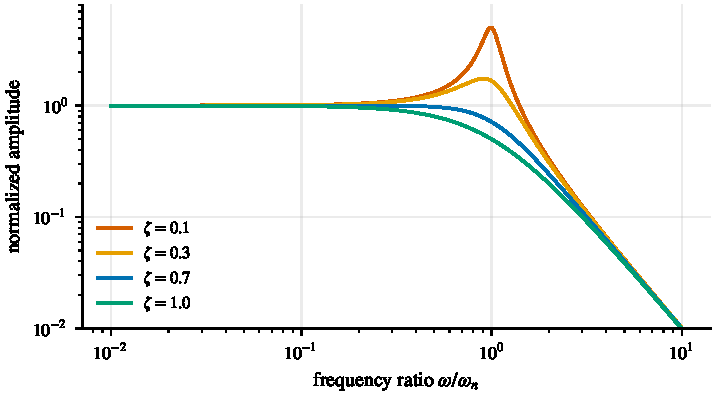
\includegraphics[width=0.84\textwidth]{fig_accel_bode.pdf}
  \caption{Frequency response of the spring-mass accelerometer model for several damping ratios. Below the natural frequency the response is flat: the
  deflection is proportional to specific force. A damping ratio near 0.7 gives the widest flat band without a resonant peak.}
  \label{fig:accel-bode}
\end{figure}

\subsection{Specific force}

\index{specific force}
The quantity measured is the \term{specific force}
\begin{equation}
  f = a - g,
\end{equation}
the non-gravitational force per unit mass acting on the sensor (the spring force divided by $m$). Gravity acts on the mass and the case equally
and cannot be felt directly: this is Einstein's equivalence principle. Two cases build intuition.
\begin{itemize}
  \item \textbf{At rest on a table}, $a = 0$, so $f = -g$. With $g_w = [0, 0, -9.81]\T$, the accelerometer reads $+9.81~\mathrm{m/s^2}$ \emph{upward}: it senses the table
        pushing it up.
  \item \textbf{In free fall}, $a = g$, so $f = 0$. A falling IMU reads zero, whatever its velocity.
\end{itemize}
To recover the kinematic acceleration from the measurement, the estimator rotates the specific force into the world frame and \emph{adds gravity back}:
$a_w = R_{wb}f_b + g_w$. A sign error here produces a vertical acceleration error of $2g \approx 20~\mathrm{m/s^2}$ and an obviously diverging altitude, which is
fortunately easy to recognize.

\paragraph{Noise.} Even a perfect mechanical sensor is noisy: the proof mass is jostled by the thermal motion of the surrounding gas, a
\emph{thermo-mechanical} noise whose acceleration density is about $\sqrt{4k_BT\omega_n/(mQ)}$ (with $k_B$ Boltzmann's constant, $T$ the temperature and $Q$ the
mechanical quality factor). Tiny masses are noisier, which is the basic trade-off of MEMS inertial sensing. Readout electronics add their own noise.

% ==============================================================================
\section{How a MEMS gyroscope works}

A MEMS \term{gyroscope} has no spinning wheel. It keeps a proof mass vibrating and detects the Coriolis force that rotation induces. Let the mass be
driven along the $x$-axis of the sensor at frequency $\omega_d$, so its velocity relative to the sensor is $v = A\omega_d\cos(\omega_dt)\,e_x$. If the sensor
rotates with angular velocity $\Omega$, then in the sensor frame the mass experiences the Coriolis acceleration $-2\Omega\times v$ (\cref{eq:coriolis}).
For a rotation about the $z$-axis this acceleration points along $y$:
\begin{equation}
  a_y = -2\,\Omega_z\,A\omega_d\cos(\omega_dt) .
\end{equation}
The resulting vibration along $y$ (the \emph{sense} mode) has an amplitude proportional to the rate $\Omega_z$ and oscillates at the drive frequency, so
the electronics recover $\Omega_z$ by demodulating the sense signal synchronously with the drive. The sensitive axis is perpendicular to both the drive and
the sense directions.

Real designs use two or four masses vibrating in anti-phase (a \emph{tuning fork}): their Coriolis forces are opposite and add in the differential
readout, while linear accelerations and vibrations push all masses the same way and cancel. Imperfect cancellation leaves a small sensitivity of the
gyro output to acceleration ($g$-sensitivity). Manufacturing asymmetries couple the drive into the sense mode (\emph{quadrature}), and their drift with
temperature is a major source of gyro bias.

% ==============================================================================
\section{The measurement model}

\subsection{The project's model}

\begin{convention}[IMU model, AGENTS.md C6]
\begin{equation}
  \omega_m = \omega_b + b_g + n_g, \qquad
  a_m = R_{wb}\T\big(a_w - g_w\big) + b_a + n_a, \qquad
  \dot b_g = n_{b_g}, \quad \dot b_a = n_{b_a},
  \label{eq:imu-model}
\end{equation}
with $\omega_m$, $a_m$ the gyroscope and accelerometer readings in the body frame, $\omega_b$ the true angular rate, $a_w$ the true acceleration of the body in the
world frame, $b_g$, $b_a$ the biases (body frame), and $n_g, n_a, n_{b_g}, n_{b_a}$ zero-mean white noises with densities $\sigma_g, \sigma_a, \sigma_{b_g}, \sigma_{b_a}$. The
noise vector is ordered $w = [n_a, n_g, n_{b_a}, n_{b_g}] \in \R^{12}$.
\end{convention}

The model has two kinds of error. \emph{White noise} ($n_g$, $n_a$) is independent from sample to sample and averages out. \emph{Bias} ($b_g$, $b_a$) is a slowly
varying offset that does not average out and is therefore estimated as part of the state (a shaping filter, \cref{ch:processes}). Its slow drift is
modeled as a random walk driven by $n_{b_g}$, $n_{b_a}$. Over the minutes of a EuRoC sequence the biases change little but measurably.

\subsection{A fuller error model}

High-accuracy inertial systems use a richer model, of which \eqref{eq:imu-model} is the special case $S = M = G = 0$:
\begin{equation}
  a_m = (I + S_a)M_a\,f_b + b_a + n_a, \qquad \omega_m = (I + S_g)M_g\,\omega_b + G_g\,f_b + b_g + n_g .
\end{equation}
Here $S$ is a diagonal matrix of \emph{scale-factor} errors (the output is $(1 + s)$ times the input), $M$ a near-identity matrix describing \emph{axis
misalignment and non-orthogonality} (the three sensing axes are neither exactly perpendicular nor exactly aligned with the body frame), and $G_g$ the
$g$-sensitivity of the gyroscope. Each of these parameters can be calibrated, estimated online as additional states, or ignored, at the cost of
some unmodeled error.

\begin{table}[t]
\centering\small
\begin{tabularx}{\textwidth}{@{}l X l@{}}
\toprule
\textbf{Error} & \textbf{Description} & \textbf{In the model?} \\
\midrule
White noise & sample-to-sample electronic and thermo-mechanical noise (angle/velocity random walk) & yes, $n_g$, $n_a$ \\
Turn-on bias & constant offset that differs at each power-up & yes, initial $b$ and $P_0$ \\
In-run bias drift & slow wandering of the offset & yes, random walk \\
Bias instability & flicker ($1/f$) noise floor of the bias & approximated by the random walk \\
Scale factor & output $= (1 + s)\times$ input & no \\
Axis misalignment & sensing axes not exactly orthogonal / aligned with the case & no \\
$g$-sensitivity & gyro output depends on acceleration & no \\
Temperature effects & bias and scale factor change with temperature & no (absorbed by bias walk) \\
Quantization & finite resolution of the ADC & no (below white noise) \\
Saturation, vibration & clipping on impacts; aliasing of high-frequency vibration & no \\
Earth rotation & gyros sense $7.3\times10^{-5}$~rad/s & no (\cref{ch:rotations}) \\
\bottomrule
\end{tabularx}
\caption{IMU error sources and how the project's model treats them.}
\label{tab:imu-errors}
\end{table}

\Cref{tab:imu-errors} lists the main error sources. Unmodeled errors do not disappear: they appear as apparent extra noise or apparent bias drift. A filter
that ignores them must compensate with larger noise parameters than the white-noise floor alone would suggest, which is why tuning is needed even with a
well-calibrated sensor. The size of the effect is easy to estimate: a scale-factor error of $10^{-3}$ on a gyro turning at 1~rad/s is an apparent bias of
$10^{-3}$~rad/s, as large as a poor bias and much larger than the EuRoC gyro's noise.

% ==============================================================================
\section{Calibration}

\paragraph{Gyroscope bias.} At rest, the gyroscope should read zero (or the Earth rate). Averaging a few seconds of data gives the bias, with a standard
deviation of $\sigma_g/\sqrt T$ after $T$ seconds (\cref{ch:processes}): for EuRoC, $10^{-4}$~rad/s after 3~s.

\paragraph{Accelerometer bias and scale: the six-position test.} Place the IMU with each axis pointing straight up and then straight down. For an axis with
bias $b$ and scale factor $1 + s$, the two readings are $(1 + s)g + b$ and $-(1 + s)g + b$, so
\begin{equation}
  b = \frac{a_{\mathrm{up}} + a_{\mathrm{down}}}{2}, \qquad 1 + s = \frac{a_{\mathrm{up}} - a_{\mathrm{down}}}{2g} .
\end{equation}
Using more orientations and a least-squares fit (\cref{ch:estimation}) also yields the misalignments.

\paragraph{Gyroscope scale and misalignment.} These require known rotations, from a rate table, or from a known sequence of orientations measured by an
accelerometer.

\paragraph{Camera--IMU calibration.} The extrinsic transform $T_{bc}$, the time offset between the sensors, and optionally the IMU's own scale and misalignment
are estimated jointly by moving the rig in front of a calibration target. The Kalibr toolbox~\cite{furgale2013kalibr}, which produced EuRoC's calibration,
represents the trajectory as a continuous-time B-spline and solves one large nonlinear least-squares problem (\cref{ch:nlls}) combining camera
reprojection errors and IMU residuals.

\paragraph{Temperature.} Biases and scale factors depend on temperature. Industrial IMUs are calibrated at several temperatures and compensated with an
on-board temperature sensor; consumer IMUs often are not, and a filter must track the resulting drift as bias random walk.

% ==============================================================================
\section{Noise parameters and their units}

The noise densities are continuous-time quantities (\cref{sec:ct-noise}). For EuRoC's ADIS16448, the \code{imu0/sensor.yaml} file gives the values in
\cref{tab:euroc-imu}.

\begin{table}[h]
\centering\small
\begin{tabular}{@{}l l l l@{}}
\toprule
YAML key & Symbol & Value & Units \\
\midrule
\code{gyroscope\_noise\_density} & $\sigma_g$ & $1.6968\times10^{-4}$ & $\mathrm{rad/s/\sqrt{Hz}}$ \\
\code{accelerometer\_noise\_density} & $\sigma_a$ & $2.0\times10^{-3}$ & $\mathrm{m/s^2/\sqrt{Hz}}$ \\
\code{gyroscope\_random\_walk} & $\sigma_{b_g}$ & $1.9393\times10^{-5}$ & $\mathrm{rad/s^2/\sqrt{Hz}}$ \\
\code{accelerometer\_random\_walk} & $\sigma_{b_a}$ & $3.0\times10^{-3}$ & $\mathrm{m/s^3/\sqrt{Hz}}$ \\
\code{rate\_hz} & $1/\Dt$ & 200 & Hz \\
\bottomrule
\end{tabular}
\caption{EuRoC IMU noise parameters (\code{imu0/sensor.yaml}). Verify against your copy of the dataset.}
\label{tab:euroc-imu}
\end{table}

The units follow from the definitions. A gyro rate in rad/s with a white noise density has units $\mathrm{rad/s}\cdot\sqrt{\mathrm{s}} = \mathrm{rad/s/\sqrt{Hz}}$. A gyro
bias random walk is the integral of white noise with units of $\mathrm{rad/s^2}$, so its density is in $\mathrm{rad/s^2/\sqrt{Hz}}$, and after $t$ seconds the
bias has standard deviation $\sigma_{b_g}\sqrt t$ in rad/s.

\paragraph{Discrete equivalents.} At sample period $\Dt$ (\cref{eq:discrete-noise}):
\begin{equation}
  \sigma_{g,d} = \frac{\sigma_g}{\sqrt\Dt}, \qquad \sigma_{a,d} = \frac{\sigma_a}{\sqrt\Dt}, \qquad
  \sigma_{b_g,d} = \sigma_{b_g}\sqrt\Dt, \qquad \sigma_{b_a,d} = \sigma_{b_a}\sqrt\Dt .
\end{equation}
For EuRoC: $\sigma_{g,d} = 2.4\times10^{-3}$~rad/s per sample, $\sigma_{a,d} = 2.8\times10^{-2}~\mathrm{m/s^2}$ per sample, and the gyro bias diffuses by
$1.4\times10^{-6}$~rad/s per sample. In the filter you never need these directly, because $Q_d = G_cQ_cG_c\T\Dt$ uses the densities, but they are what a synthetic
data generator must add to each sample.

\paragraph{Datasheet units.} Manufacturers often quote angle random walk (ARW) in $^\circ/\sqrt{\mathrm{h}}$ and velocity random walk (VRW) in $\mathrm{m/s/\sqrt{h}}$.
Since $1\ ^\circ/\sqrt{\mathrm{h}} = \frac{\pi/180}{60}~\mathrm{rad/\sqrt{s}} = 2.909\times10^{-4}~\mathrm{rad/s/\sqrt{Hz}}$, EuRoC's $\sigma_g$ is an ARW of $0.58\ ^\circ/\sqrt{\mathrm{h}}$,
and its $\sigma_a$ is a VRW of $0.12~\mathrm{m/s/\sqrt{h}}$. Bias instability is quoted in $^\circ/\mathrm{h}$ and is \emph{not} the same thing as the random walk
density.

\paragraph{Measuring them.} The densities are measured from a long static recording with the Allan variance (\cref{sec:allan,fig:allan}): white noise is read
off the slope $-\tfrac12$ at $\tau = 1$~s, and the bias random walk off the slope $+\tfrac12$ at $\tau = 3$~s.

% ==============================================================================
\section{Tuning in practice}

The densities from an Allan analysis describe a stationary sensor in a quiet lab. On a flying vehicle, vibration, temperature changes, scale-factor and
misalignment errors, timing jitter and integration error all add to the effective noise. Common practice is to start from the Allan values (or the
dataset's values) and inflate them by a modest factor until the filter is consistent, as judged by the statistical tests of \cref{ch:consistency}. Two
rules keep tuning honest.
\begin{enumerate}
  \item \textbf{Change physically meaningful parameters only}, and keep them within a plausible range of their measured values.
  \item \textbf{Judge on consistency statistics} (NEES on synthetic data, NIS and $3\sigma$ coverage on real data), not on trajectory error alone. Tuning for
        the lowest trajectory error on the test sequence is overfitting.
\end{enumerate}

\begin{pitfall}[mixing up the two discretizations]
The white-noise variance per sample is $\sigma^2/\Dt$ (larger at higher rate), while the random-walk variance per step is $\sigma_b^2\Dt$ (smaller at higher rate).
Swapping them is a common bug in synthetic data generators, and it produces noise that is wrong by a factor of $1/\Dt^2 = 40\,000$ at 200~Hz.
\end{pitfall}

\section{The EuRoC IMU stream}

EuRoC's \code{imu0/data.csv} contains one row per sample: \code{timestamp [ns], w\_x, w\_y, w\_z [rad/s], a\_x, a\_y, a\_z [m/s\textsuperscript{2}]}, i.e.\ $\omega_m$
and $a_m$ in $B$ (AGENTS.md C7). Samples arrive at nominally 200~Hz, hardware-synchronized with the cameras. The filter must nevertheless take $\Dt$ from
consecutive timestamps (AGENTS.md C5): real data has jitter and occasional gaps, which Milestone 3 logs. The ground-truth file starts later than the IMU
file, so the filter is initialized at the first ground-truth sample at or after the stream start.

\begin{projectlink}[Milestones 3 and 4]
M3 parses \code{sensor.yaml} into exactly the parameters of \cref{tab:euroc-imu} and builds the event stream. M4's synthetic trajectory generator produces
noise-free IMU data from \eqref{eq:imu-model}; adding noise with the discrete equivalents above turns it into the Monte Carlo generator of M5.
\end{projectlink}

\begin{takeaways}
\begin{itemize}
  \item An accelerometer is a spring-mass system whose deflection, below resonance, is proportional to specific force $f = a - g$: it reads $+g$ upward at rest
        and zero in free fall.
  \item A MEMS gyroscope measures the Coriolis force on a vibrating mass.
  \item $\omega_m = \omega_b + b_g + n_g$ and $a_m = R_{wb}\T(a_w - g_w) + b_a + n_a$, with random-walk biases; scale factors and misalignments are neglected.
  \item Biases and scale factors can be calibrated with static multi-position tests; camera--IMU extrinsics with a target and a continuous-time solver.
  \item Noise densities have units of $[u]/\sqrt{\mathrm{Hz}}$; per-sample white noise is $\sigma/\sqrt\Dt$, per-step bias diffusion is $\sigma_b\sqrt\Dt$.
  \item Unmodeled errors force noise inflation; tune on consistency, not on accuracy.
\end{itemize}
\end{takeaways}

\begin{exercises}
  \item An IMU lies on a table tilted by $10^\circ$ about its $x$-axis. Compute the ideal accelerometer reading. Which component reveals the tilt, and with what sign?
  \item A MEMS accelerometer has a resonance at 5~kHz. How large is its static deflection per $\mathrm{m/s^2}$? Compare with the size of a silicon atom
        ($\approx 0.2$~nm) and comment.
  \item Derive the gyroscope's Coriolis acceleration from \eqref{eq:coriolis}, and explain why a tuning-fork design rejects linear acceleration.
  \item A six-position test gives $a_{\mathrm{up}} = 9.83$ and $a_{\mathrm{down}} = -9.79~\mathrm{m/s^2}$ on one axis. Compute the bias and scale factor.
  \item A gyroscope datasheet gives ARW $= 0.2\ ^\circ/\sqrt{\mathrm{h}}$. Convert it to $\mathrm{rad/s/\sqrt{Hz}}$ and to the per-sample standard deviation at 400~Hz.
  \item A scale-factor error of $s = 10^{-3}$ affects a gyro on a vehicle spinning at 1~rad/s. What equivalent bias does it produce? Why can't a constant-bias model
        absorb it during maneuvers?
\end{exercises}

\chapter{Strapdown Propagation of the Nominal State}
\label{ch:strapdown}
\chaptermark{Strapdown Propagation} % short running header

\begin{objectives}
\begin{itemize}
  \item State the continuous-time nominal kinematics and understand each term.
  \item Derive the exact solution of the kinematics for constant inputs over a step.
  \item Compare Euler, midpoint and Runge--Kutta integration, and predict their convergence orders.
  \item Propagate to arbitrary timestamps, handle gaps, and initialize the nominal state.
  \item Understand IMU preintegration as used by optimization-based estimators.
\end{itemize}
\end{objectives}

A \emph{strapdown} inertial system has its sensors rigidly attached (strapped down) to the vehicle, as
opposed to mounted on a stabilized gimbal platform. All the work of keeping track of orientation is done in
software, by integrating the gyroscope. This chapter is about that integration.

% ------------------------------------------------------------------------------
\section{Continuous-time kinematics}

\subsection{The navigation equations}

\index{strapdown mechanization}
The \emph{mechanization equations} follow from three facts established earlier. The position changes with the velocity, $\dot p_{wb} = v_{wb}$. The
velocity changes with the acceleration, which by the definition of specific force (\cref{ch:imu}) is the measured specific force rotated into the world
frame plus gravity, $\dot v_{wb} = a_w = R_{wb}f_b + g_w$. And the attitude changes with the body angular velocity, $\dot R_{wb} = R_{wb}\sx{\omega_b}$
(\cref{sec:rot-kinematics}). Here the world frame is treated as inertial, with the effects of the Earth's rotation neglected or absorbed into gravity
and the gyro bias; \cref{ch:rotations} showed that they are tiny over the scales of a EuRoC flight. Substituting the IMU model,
$f_b = a_m - b_a - n_a$ and $\omega_b = \omega_m - b_g - n_g$, gives the true kinematics of \cref{ch:errordyn}, and replacing the unknown biases by their estimates and
setting the noise to zero gives the nominal kinematics.

\begin{convention}[nominal propagation, AGENTS.md F1]
\begin{equation}
  \hat a = a_m - \hat b_a,\quad \hat\omega = \omega_m - \hat b_g;\qquad
  \dot{\hat p} = \hat v,\quad \dot{\hat v} = \hat R_{wb}\,\hat a + g_w,\quad
  \dot{\hat q} = \tfrac12\,\hat q\qprod[0,\ \hat\omega],\quad \dot{\hat b}_a = \dot{\hat b}_g = 0 .
  \label{eq:nominal-ct}
\end{equation}
The attitude update is always multiplicative, $\hat q \gets \hat q\qprod\Exp_q(\hat\omega\Dt)$, followed by
normalization. The integration scheme for $p$ and $v$ is chosen and justified in Milestone 4 and logged
in \texttt{PROGRESS.md}.
\end{convention}

The equations form a cascade: attitude depends on the gyroscope only; velocity depends on attitude and the
accelerometer; position depends on velocity. Errors cascade the same way, which is the origin of the
$t^2$ and $t^3$ growth laws of \cref{ch:intro}.

% ------------------------------------------------------------------------------
\section{Exact solution for constant inputs}

Suppose $\hat\omega$ and $\hat a$ are constant over $[t_k, t_k + \Dt]$, which is what a zero-order hold of one
IMU sample assumes. Then the kinematics can be solved in closed form.

\begin{proposition}[Constant-input propagation]
\label{prop:exact-prop}
With $\hat\omega$, $\hat a$ constant over the step and $\phi = \hat\omega\Dt$,
\begin{align}
  \hat R_{k+1} &= \hat R_k\,\Exp(\phi), \\
  \hat v_{k+1} &= \hat v_k + g_w\Dt + \hat R_k\,\Dt\,\Jl(\phi)\,\hat a, \\
  \hat p_{k+1} &= \hat p_k + \hat v_k\Dt + \tfrac12 g_w\Dt^2 + \hat R_k\,\Dt^2\,N(\phi)\,\hat a,
\end{align}
where $N(\phi) = \sum_{j\ge0}\sx{\phi}^j/(j+2)! = \tfrac12 I + \frac{\theta - \sin\theta}{\theta^3}\sx{\phi} +
\frac{\theta^2/2 + \cos\theta - 1}{\theta^4}\sx{\phi}^2$ and $\theta = \|\phi\|$.
\end{proposition}
\begin{proof}
The attitude is \cref{prop:const-rate}. During the step $\hat R(t_k + s) = \hat R_k\Exp(\hat\omega s)$, so
$\hat v_{k+1} - \hat v_k = g_w\Dt + \hat R_k\int_0^\Dt\Exp(\hat\omega s)\,\dd s\,\hat a$, and
$\int_0^\Dt\Exp(\hat\omega s)\,\dd s = \Dt\int_0^1\Exp(u\phi)\,\dd u = \Dt\,\Jl(\phi)$ by \cref{thm:jr}. Integrating once more
gives the position, with $\int_0^\Dt\!\int_0^s\Exp(\hat\omega u)\,\dd u\,\dd s = \Dt^2N(\phi)$ by term-wise integration of
the exponential series, and the closed form follows from $\sx{\phi}^3 = -\theta^2\sx{\phi}$.
\end{proof}

For small $\phi$, $\Jl(\phi) \approx I + \tfrac12\sx{\phi}$ and $N(\phi) \approx \tfrac12 I + \tfrac16\sx{\phi}$. The
correction terms account for the rotation of the specific-force vector during the step. At 200~Hz and
1~rad/s, $\|\phi\| = 0.005$, so they change the velocity increment by about 0.25\%: small, but systematic.

% ------------------------------------------------------------------------------
\section{Numerical integration schemes}

Real inputs are not constant over a step: the IMU provides samples at $t_k$ and $t_{k+1}$, and the true signal
varies between them. Three families of schemes are common. All of them update the attitude
multiplicatively.

\paragraph{Euler with zero-order hold.} Use the sample at the start of the step for the whole step:
\begin{equation}
  \hat R_{k+1} = \hat R_k\Exp(\hat\omega_k\Dt), \quad
  \hat v_{k+1} = \hat v_k + (\hat R_k\hat a_k + g_w)\Dt, \quad
  \hat p_{k+1} = \hat p_k + \hat v_k\Dt + \tfrac12(\hat R_k\hat a_k + g_w)\Dt^2 .
\end{equation}
Local error $O(\Dt^2)$, global error $O(\Dt)$. The dominant error is essentially a \emph{half-sample time
shift}: using the sample from the start of the interval for the whole interval delays the signal by
$\Dt/2$ on average. To see the local error, expand the true velocity increment $\int_{t_k}^{t_{k+1}}a_w(t)\,\dd t = a_w(t_k)\Dt + \tfrac12\dot a_w(t_k)\Dt^2 + O(\Dt^3)$; Euler keeps
only the first term, so each step errs by $\tfrac12\dot a_w\Dt^2$, and the errors of the $T/\Dt$ steps accumulate to $O(\Dt)$.

\paragraph{Midpoint (trapezoidal).} Use the average of the two bounding samples:
\begin{equation}
  \hat R_{k+1} = \hat R_k\Exp\big(\tfrac12(\hat\omega_k + \hat\omega_{k+1})\Dt\big),\quad
  \bar a_w = \tfrac12\big(\hat R_k\hat a_k + \hat R_{k+1}\hat a_{k+1}\big) + g_w,
\end{equation}
\begin{equation*}
  \hat v_{k+1} = \hat v_k + \bar a_w\Dt, \qquad \hat p_{k+1} = \hat p_k + \hat v_k\Dt + \tfrac12\bar a_w\Dt^2 .
\end{equation*}
Local error $O(\Dt^3)$, global $O(\Dt^2)$, at the cost of having to wait for the next sample before
completing the step.

\paragraph{Runge--Kutta 4.} RK4 evaluates the dynamics at the start, twice at the middle, and at the end of
the step. Its global error is $O(\Dt^4)$ \emph{if} the inputs at mid-step are known exactly. With an IMU
they are not, and must be interpolated from the bounding samples. Linear interpolation is only
second-order accurate, which caps the whole scheme at $O(\Dt^2)$.

\begin{figure}[t]
  \centering
  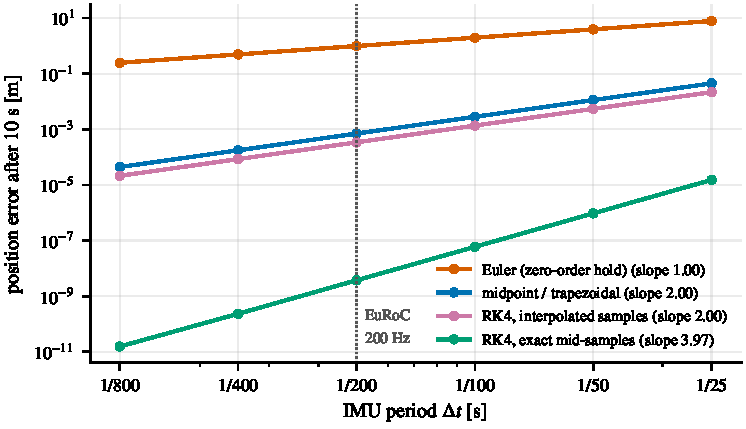
\includegraphics[width=0.86\textwidth]{fig_integration_order.pdf}
  \caption{Position error after 10~s of noise-free integration on a synthetic trajectory (2~m circle at
  0.8~rad/s with $\pm23^\circ$ roll oscillations), as a function of the IMU period. The measured slopes
  match the predicted global orders. RK4 reaches fourth order only with exact mid-step inputs, which a
  real IMU does not provide; with interpolated inputs it is no better than the midpoint rule.}
  \label{fig:integration-order}
\end{figure}

\Cref{fig:integration-order} confirms the predicted orders. Halving $\Dt$ divides the error by 2 for Euler and
by 4 for the midpoint rule, which is exactly the convergence-order test of Milestone 4. The magnitudes
matter as much as the slopes. At 200~Hz on this fairly dynamic trajectory, the Euler scheme accumulates
about a meter of error in 10~s, far more than the sensor noise would cause (\cref{fig:cov-growth}), because the
half-sample delay of the attitude creates a tilt error of order $\tfrac12\omega\Dt$, which leaks gravity. The
midpoint rule is three orders of magnitude better. On gentler motion the difference shrinks, and frequent
visual updates bound integration error in any case, but the integration error should be well below the
noise-induced error, or it becomes an unmodeled error that the filter cannot account for.

\begin{keyidea}[choosing a scheme]
The integration error is a deterministic, unmodeled error. The scheme should make it small compared with
the stochastic error the filter does model. Whichever scheme Milestone 4 adopts, document its order and
verify it with the halving test on a trajectory with closed-form ground truth.
\end{keyidea}

% ------------------------------------------------------------------------------
\section{Coning, sculling and the rotation-vector equation}
\label{sec:coning}

\subsection{The rotation vector of a step}

The attitude update over a step is a rotation $\Delta R = R(t_k)\T R(t_{k+1})$, which we can write as $\Exp(\phi)$ for a rotation vector $\phi$. If the angular
velocity keeps a fixed direction during the step, $\phi = \int\omega\,\dd t$. If its direction changes, this is wrong (\cref{prop:stm}), and the correct $\phi$
obeys a differential equation of its own.

\begin{proposition}[Bortz equation]
\label{prop:bortz}
\index{Bortz equation}
The rotation vector $\phi(t)$ with $\Exp(\phi(t)) = R(t_k)\T R(t)$ satisfies
\begin{equation}
  \dot\phi = \Jrinv(\phi)\,\omega = \omega + \tfrac12\,\phi\times\omega + D(\|\phi\|)\,\phi\times(\phi\times\omega),
\end{equation}
with $D$ the coefficient function of \cref{thm:jr}.
\end{proposition}
\begin{proof}
Over an instant $\dd t$, $\Exp(\phi + \dot\phi\,\dd t) = \Exp(\phi)\Exp(\omega\,\dd t)$. By the definition of the right Jacobian \eqref{eq:jr-def}, the left side is
$\Exp(\phi)\Exp(\Jr(\phi)\dot\phi\,\dd t)$, so $\Jr(\phi)\dot\phi = \omega$. Expand $\Jrinv$ with \eqref{eq:jrinv}.
\end{proof}

The term $\tfrac12\phi\times\omega$ is non-zero only when $\omega$ is not parallel to the rotation already accumulated: it is the \emph{non-commutativity
correction}. Under \emph{coning motion}, in which the angular velocity vector itself rotates (for example $\omega = (a\cos\Omega t,\ a\sin\Omega t,\ 0)$, the motion of
a vibrating or wobbling body), this correction does not average to zero. Integrating the rate vector alone then produces a steady, spurious
rotation about the cone axis, a drift that no amount of averaging removes.

\subsection{The two-sample coning correction}

Given the integrated gyro increments $\alpha_1$ and $\alpha_2$ over the two halves of a step (which a high-rate IMU, or two consecutive samples, provides),
the rotation vector of the whole step is, to third order,
\begin{equation}
  \phi \approx \alpha_1 + \alpha_2 + \tfrac23\,\alpha_1\times\alpha_2 .
  \label{eq:coning}
\end{equation}
\begin{proof}[Derivation]
Keep the first-order Bortz equation $\dot\phi \approx \omega + \tfrac12\phi\times\omega$ and suppose the rate varies linearly over the step, $\omega(s) = a + bs$ for
$s \in [0, h]$. To the needed order $\phi(s) \approx \int_0^s\omega = as + \tfrac12bs^2$, so
\begin{align*}
  \phi(h) &\approx \int_0^h\omega\,\dd s + \frac12\int_0^h\big(as + \tfrac12bs^2\big)\times(a + bs)\,\dd s \\
       &= \int_0^h\omega\,\dd s + \frac12(a\times b)\int_0^h\big(s^2 - \tfrac12s^2\big)\dd s
       = \alpha_1 + \alpha_2 + \frac{h^3}{12}\,a\times b .
\end{align*}
The half-step increments are $\alpha_1 = \tfrac h2a + \tfrac{h^2}8b$ and $\alpha_2 = \tfrac h2a + \tfrac{3h^2}8b$, whose cross product is $\alpha_1\times\alpha_2 = \tfrac{h^3}8\,a\times b$.
Hence $\tfrac{h^3}{12}a\times b = \tfrac23\alpha_1\times\alpha_2$.
\end{proof}

\begin{figure}[t]
  \centering
  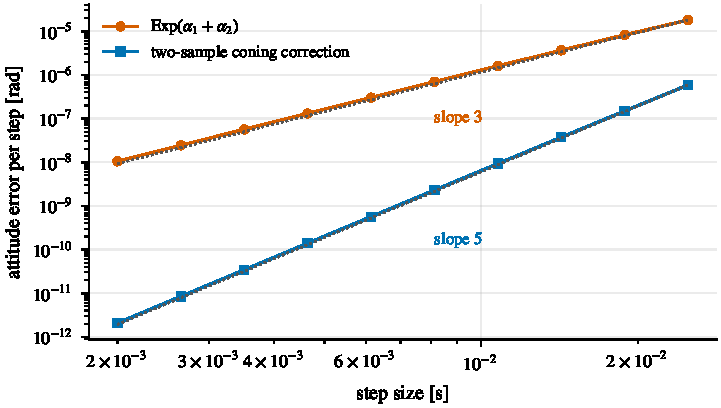
\includegraphics[width=0.84\textwidth]{fig_coning.pdf}
  \caption{Attitude error over one step under coning motion (rate amplitude 0.5~rad/s, coning frequency 10~Hz), as a function of the step size.
  Exponentiating the integrated rate errs at third order; the two-sample correction \eqref{eq:coning} reduces the error to fifth order.}
  \label{fig:coning}
\end{figure}

\Cref{fig:coning} confirms the orders. \emph{Sculling} is the analogous effect for velocity: when rotation and acceleration oscillate in phase, the
specific force is rotated while it is being integrated, and the error rectifies into a velocity drift; it has similar multi-sample corrections. High-end
inertial systems, with gyros sampled at kHz rates on vibrating platforms, rely on such algorithms~\cite{groves2013principles}. For a MEMS IMU sampled at
200~Hz, with vibration filtered by the sensor's own electronics, the effects are small compared with the sensor noise, and the project's single-sample
schemes suffice. The analysis still matters: it tells you what you are neglecting, and how to check that it is negligible.

% ------------------------------------------------------------------------------
\section{Timing}

\subsection{Propagating to an arbitrary time}

Images arrive between IMU samples. To clone the state at an image time $t_c \in (t_k, t_{k+1})$ (AGENTS.md F5), the
filter must propagate exactly to $t_c$: interpolate the IMU reading at $t_c$ linearly between samples $k$ and
$k+1$, propagate from $t_k$ to $t_c$ with the interpolated input, clone, and then propagate from $t_c$ to $t_{k+1}$.
The covariance follows the same split, with $\Dt$ replaced by the two partial intervals.

\subsection{Event ordering and gaps}

Measurements must be processed in timestamp order, and the state must be propagated to a measurement's time
before the measurement is applied (\cref{ch:fullalgo}). Milestone 3 fixes the tie rule: an IMU sample precedes a
measurement with an equal timestamp, so the state is propagated to that time first. Gaps in the IMU stream
(intervals larger than about $1.5$ nominal periods) must not be assumed away. $\Dt$ always comes from the
timestamps, and a long gap simply produces a long step with a correspondingly large $Q_d$.

% ------------------------------------------------------------------------------
\section{Initialization}

\subsection{From ground truth}

The project initializes the nominal state from the first ground-truth sample at or after the start of the
stream (Milestone 4): $p$, $v$, $q$, $b_a$ and $b_g$ all come from the ground-truth columns, mapped with the
column order of AGENTS.md C7. This isolates propagation from the initialization problem. The use of ground
truth for initialization is logged when the full VIO runs (Milestone 10b).

\subsection{Static initialization}

A real system initializes from its own sensors. If the vehicle is at rest for about a second,
\begin{equation}
  \bar a_m = \mathrm{mean}(a_m) \approx R_{wb}\T(-g_w) + b_a, \qquad \bar\omega_m = \mathrm{mean}(\omega_m) \approx b_g .
\end{equation}
The gyro bias is the mean rate. Neglecting $b_a$, the unit vector $u_b = \bar a_m/\|\bar a_m\|$ is the world
``up'' direction expressed in the body frame, $u_b = R_{wb}\T e_z$. Any rotation with $R_{wb}u_b = e_z$ is consistent
with it. One such rotation turns $u_b$ onto $e_z$ about the axis perpendicular to both:
\begin{equation}
  R_{wb} = \Exp\!\Big(\atantwo\big(\|u_b\times e_z\|,\ u_b\T e_z\big)\,\frac{u_b\times e_z}{\|u_b\times e_z\|}\Big),
\end{equation}
(with $R_{wb} = I$ if $u_b = e_z$ already), and composing it on the left with any rotation $R_z(\psi)$ about the vertical gives all the others. Roll and pitch are
determined; yaw is arbitrary, and is set to zero (or to the ground-truth yaw for evaluation).

\begin{pitfall}[tilt and accelerometer bias are indistinguishable at rest]
A horizontal accelerometer bias $b_a$ produces the same reading as a tilt of $\|b_a\|/g$: a bias of
$10~\mathrm{mm/s^2}$ looks exactly like a tilt of $1$~mrad. At rest the filter cannot separate them, and the initial
covariance must say so (large $\sigma_{b_a}$, correlated with the tilt). They become separable once the vehicle
rotates, because the bias rotates with the body while gravity does not.
\end{pitfall}

Initial covariances should reflect real uncertainty: a few milliradians in roll and pitch, a large or
unknown yaw, the turn-on bias range from the datasheet, and a small but non-zero velocity uncertainty at rest.
\emph{Dynamic} initialization from a moving start, as in VINS-Mono~\cite{qin2018vins}, first solves a
vision-only structure-from-motion problem and then aligns it with preintegrated IMU data to recover scale,
gravity and velocity.

% ------------------------------------------------------------------------------
\section{Sidebar: IMU preintegration}

An optimization-based estimator may relinearize a window of states many times. Re-integrating every IMU
sample between keyframes $i$ and $j$ each time the estimate of state $i$ changes would be wasteful.
\emph{Preintegration}~\cite{lupton2012visual, forster2017preintegration} integrates the measurements in the body frame
of keyframe $i$, so that the result does not depend on the state at $i$:
\begin{equation}
  \Delta R_{ij} = \prod_{k=i}^{j-1}\Exp(\hat\omega_k\Dt), \quad
  \Delta v_{ij} = \sum_{k=i}^{j-1}\Delta R_{ik}\,\hat a_k\Dt, \quad
  \Delta p_{ij} = \sum_{k=i}^{j-1}\Big(\Delta v_{ik}\Dt + \tfrac12\Delta R_{ik}\,\hat a_k\Dt^2\Big).
\end{equation}
These relate the two keyframe states through
$R_j = R_i\Delta R_{ij}$, $v_j = v_i + g\Delta t_{ij} + R_i\Delta v_{ij}$ and
$p_j = p_i + v_i\Delta t_{ij} + \tfrac12g\Delta t_{ij}^2 + R_i\Delta p_{ij}$. The preintegrated quantities depend on the
bias estimate, and first-order bias Jacobians avoid re-integration when the bias estimate changes. A filter
like the MSCKF does not need preintegration, because it integrates each sample exactly once.

\begin{projectlink}[Milestone 4]
Exit criteria: a stationary input keeps the state constant to $10^{-9}$ for 60~s; a constant rate reproduces
$q_0\qprod\Exp_q(\omega t)$; a circular trajectory converges at the predicted order; the quaternion norm stays
within $10^{-12}$ of one after $10^6$ steps; propagation does not allocate; and 10~s of dead reckoning on
MH\_01 produce no NaN.
\end{projectlink}

\begin{takeaways}
\begin{itemize}
  \item $\dot p = v$, $\dot v = R\hat a + g$, $\dot q = \tfrac12 q\qprod[0,\hat\omega]$; attitude updates are multiplicative.
  \item For constant inputs the solution is exact: $R\Exp(\phi)$, $v + g\Dt + R\Dt\Jl(\phi)\hat a$, and a similar
        position formula.
  \item Euler is first order (a half-sample delay), midpoint second order. RK4 is limited to second order by
        input interpolation.
  \item Integration error is unmodeled error; keep it well below sensor-noise error and verify the order.
  \item Propagate exactly to measurement times by splitting the IMU interval.
  \item At rest, gravity gives roll and pitch, the mean gyro gives $b_g$, and tilt and horizontal $b_a$ are
        indistinguishable.
\end{itemize}
\end{takeaways}

\begin{exercises}
  \item Verify \cref{prop:exact-prop} numerically by comparing with an ODE solver at tight tolerance.
  \item Show that the Euler scheme applied to a constant rotation rate is exact for the attitude, but not for
        the velocity, and quantify the velocity error per step in terms of $\|\hat\omega\|\Dt$.
  \item Reproduce \cref{fig:integration-order}. Then add gyro noise and plot the noise-induced position error
        on the same axes. At what IMU rate does integration error fall below noise error for each scheme?
  \item Implement the static initializer and test it on synthetic data with a known tilt. Add a horizontal
        accelerometer bias and show that it biases the estimated tilt by $\|b_a\|/g$.
  \item Why must the propagation to an image timestamp interpolate the IMU sample instead of using the
        nearest sample? Estimate the attitude error from using the nearest sample at 1~rad/s and 200~Hz.
\end{exercises}
% Solutions to the exercises of Chapter 16.
\begin{solutions}
  \item Choose a non-trivial initial state ($R_0 = \Exp(0.2, -0.1, 0.4)$, $v_0 = (1, 0.5, -0.2)$, $p_0 = (0.1, 0.2, 0.3)$), constant inputs
        $\hat\omega = (0.3, -0.5, 0.8)$~rad/s and $\hat a = (1, -2, 9)~\mathrm{m/s^2}$, and a long step $\Dt = 0.5$~s so that $\|\phi\| = 0.5$~rad and the correction terms
        are large. Integrating $\dot R = R\sx{\hat\omega}$, $\dot v = R\hat a + g_w$, $\dot p = v$ with \code{scipy.integrate.solve\_ivp} (DOP853, tolerances $10^{-13}$) and
        comparing with \cref{prop:exact-prop} gives differences of $2\times10^{-15}$ in $R$ and $8\times10^{-15}$ in $v$ and $p$: the closed forms are exact. Setting
        $\Jl = I$ and $N = \tfrac12I$ instead produces errors of order $\tfrac12\|\phi\|\,\|\hat a\|\Dt$, many orders of magnitude larger.

  \item With constant $\hat\omega$ the Euler scheme's attitude update $\hat R_k\Exp(\hat\omega\Dt)$ is exactly \cref{prop:const-rate}. Its velocity update uses
        $\hat R_k\hat a\,\Dt$, while the exact increment is $\hat R_k\Dt\Jl(\phi)\hat a$ with $\Jl(\phi) = I + \tfrac12\sx{\phi} + O(\|\phi\|^2)$. The error per step is
        \[
          \hat R_k\Dt\big(\Jl(\phi) - I\big)\hat a = \tfrac12\hat R_k\,\Dt^2\,\hat\omega\times\hat a + O(\Dt^3),
        \]
        a fraction $\tfrac12\|\hat\omega\|\Dt\sin\angle(\hat\omega, \hat a)$ of the step's velocity increment: $0.25\%$ at 1~rad/s and 200~Hz (a numerical check gives
        exactly $0.0025$). It is the effect of holding the specific force fixed in the body frame at the start of the step while the body rotates;
        it is systematic, so it accumulates.

  \item Running the code of \cref{fig:integration-order} gives position errors after 10~s at 200~Hz of $1.0$~m (Euler), $7\times10^{-4}$~m (midpoint) and
        $3\times10^{-4}$~m (RK4 with interpolated mid-samples), each scaling with its order. Adding EuRoC's gyro and accelerometer white noise to the
        samples and repeating 40 times gives a noise-induced RMS position error of about $0.17$--$0.19$~m after 10~s, the same at 100, 200 and 800~Hz:
        sampling faster does not reduce the noise per unit time (\cref{sec:ct-noise}). The noise error is therefore a horizontal line on the plot, and
        each integration error curve crosses it where:
        \begin{itemize}[leftmargin=1.2em]
          \item Euler: its error $\approx 1.0~\mathrm m\times(200/f)$ falls below $0.18$~m only above about $1.1$~kHz, faster than most MEMS IMUs deliver;
          \item midpoint and interpolated RK4: their errors are below the noise at every rate tested, down to 25~Hz ($0.045$ and $0.022$~m).
        \end{itemize}
        At EuRoC's 200~Hz a second-order scheme makes the integration error two to three orders of magnitude smaller than the noise, which is the
        requirement of \cref{ch:strapdown}.

  \item Generate one second of static accelerometer samples at 200~Hz for a known tilt (roll $5^\circ$, pitch $-3^\circ$) with EuRoC noise, average them, and apply
        the initializer. The estimated ``up'' direction is within $0.2$~mrad of the truth (the residual is the noise of the average,
        $\sigma_a/\sqrt{1\,\mathrm s}/g$ per axis). Adding a body-frame bias $b_a = (0.05, 0, 0)~\mathrm{m/s^2}$, almost horizontal for this attitude, moves the estimate by
        $4.9$~mrad, against the prediction $\|b_{a,\perp}\|/g = 5.1$~mrad, where $b_{a,\perp}$ is the component perpendicular to gravity (the difference is the noise
        of the average). The reason: the initializer takes the direction of $R\T(-g_w) + b_a$ to be ``up''; a horizontal bias tilts that vector by
        $\arctan(\|b_{a,\perp}\|/g) \approx \|b_{a,\perp}\|/g$, and nothing in a static recording distinguishes it from a real tilt.

  \item The clone must be the pose at the image timestamp $t_c$. Propagating only to the nearest IMU sample makes the clone the pose at a time that
        differs from $t_c$ by up to half a sample period, $\Dt/2 = 2.5$~ms at 200~Hz (1.25~ms on average, for a uniformly distributed offset). At 1~rad/s
        the attitude error is up to $2.5$~mrad, comparable to the angle subtended by one pixel of the EuRoC camera ($1/458 \approx 2.2$~mrad), and at 1~m/s the
        position error is up to $2.5$~mm. Unlike pixel noise this error is not random from the filter's point of view: it is correlated with the motion,
        so it biases every visual constraint during fast rotations. Interpolating the IMU sample at $t_c$ and propagating exactly to it removes the error
        at no cost.
\end{solutions}


\chapter{Error-State Dynamics and Covariance Propagation}
\label{ch:errordyn}
\chaptermark{Error-State Dynamics} % short running header

\begin{objectives}
\begin{itemize}
  \item Set up the 15-dimensional IMU error state with the frozen index layout.
  \item Derive linearized error dynamics with the four-step recipe, including the attitude error under a
        perturbation convention.
  \item Discretize into $\Phi$ and $Q_d$ and propagate the covariance of the IMU state and its clones.
  \item Predict analytically how fast each noise source inflates the position uncertainty.
  \item Validate the propagation by finite differences and by Monte Carlo simulation.
\end{itemize}
\end{objectives}

% ------------------------------------------------------------------------------
\section{True and nominal systems}

The true state evolves under the IMU model \eqref{eq:imu-model} solved for the physical quantities. With
$\omega = \omega_m - b_g - n_g$ and $a = a_m - b_a - n_a$ the true body rate and specific force,
\begin{equation}
  \dot p = v, \qquad \dot v = R\,(a_m - b_a - n_a) + g_w, \qquad \dot R = R\,\sx{\omega_m - b_g - n_g},
  \qquad \dot b_a = n_{b_a}, \qquad \dot b_g = n_{b_g},
  \label{eq:true-ct}
\end{equation}
where $R = R_{wb}$. The nominal state follows \eqref{eq:nominal-ct}, which is \eqref{eq:true-ct} with the biases replaced
by their estimates and the noise set to zero. The error state measures their difference.

\begin{convention}[error-state layout, AGENTS.md C3]
\begin{center}\small
\begin{tabular}{@{}c c l@{}}
\toprule
Indices & Block & Meaning \\
\midrule
0--2 & $\delta p$ & position error, world frame \\
3--5 & $\delta v$ & velocity error, world frame \\
6--8 & $\delta\theta$ & attitude error, \textbf{body frame (local)}: $R = \hat R\Exp(\delta\theta)$ \\
9--11 & $\delta b_a$ & accelerometer bias error \\
12--14 & $\delta b_g$ & gyroscope bias error \\
$15+6i$ \dots $+2$ & $\delta p_i$ & clone $i$ position error \\
$18+6i$ \dots $+2$ & $\delta\theta_i$ & clone $i$ attitude error (local) \\
\bottomrule
\end{tabular}
\end{center}
Noise ordering: $w = [n_a, n_g, n_{b_a}, n_{b_g}] \in \R^{12}$.
\end{convention}

Index constants belong in one place in the code (\code{constexpr} offsets in \code{types.hpp}), and every block
access goes through them. Hard-coded literals such as \code{P.block<3,3>(6,6)} scattered through the code are how
layout bugs are born.

% ------------------------------------------------------------------------------
\section{Deriving the error dynamics}
\label{sec:deriving-Fc}

The goal is the linear system
\begin{equation}
  \dot{\delta x}_I = F_c\,\delta x_I + G_c\,w, \qquad F_c \in \R^{15\times15},\quad G_c \in \R^{15\times12},
\end{equation}
obtained with the recipe of \cref{sec:error-dyn-recipe}. Two of the five blocks are immediate.

\paragraph{Position.} Substituting $p = \hat p + \delta p$ and $v = \hat v + \delta v$ into $\dot p = v$ and subtracting
$\dot{\hat p} = \hat v$ gives $\dot{\delta p} = \delta v$ exactly. No linearization is needed.

\paragraph{Biases.} $\dot b_a = n_{b_a}$ and $\dot{\hat b}_a = 0$ give $\dot{\delta b}_a = n_{b_a}$, and likewise
$\dot{\delta b}_g = n_{b_g}$.

The velocity and attitude blocks involve the rotation and require the Lie tools of \cref{ch:lie}. One lemma
handles the time derivative of the perturbation itself.

\begin{lemma}[Time derivative of a perturbation]
\label{lem:dexp}
For a differentiable $\delta\theta(t)$,
$\frac{\dd}{\dd t}\Exp(\delta\theta) = \Exp(\delta\theta)\sx{\Jr(\delta\theta)\,\dot{\delta\theta}} = \sx{\Jl(\delta\theta)\,\dot{\delta\theta}}\Exp(\delta\theta)$.
To first order in $\delta\theta$, both reduce to $\sx{\dot{\delta\theta}}$ multiplying $\Exp(\delta\theta)$ on the corresponding side.
\end{lemma}
\begin{proof}
Apply the definition \eqref{eq:jr-def} of $\Jr$ and $\Jl$ with $\delta = \dot{\delta\theta}\,\dd t$.
\end{proof}

\subsection{Worked example: attitude error under the global perturbation}

To demonstrate the method without solving the project's exercise, we first derive the attitude error
dynamics for the \emph{global} perturbation $R = \Exp(\delta\theta_g)\hat R$. This is \textbf{not} the project's
convention; it is here for contrast.

\begin{example}[Global attitude error dynamics]
\label{ex:global-attitude}
Differentiate both sides of $R = \Exp(\delta\theta_g)\hat R$ using \cref{lem:dexp} to first order and the kinematics
$\dot R = R\sx{\omega}$, $\dot{\hat R} = \hat R\sx{\hat\omega}$:
\begin{equation*}
  \underbrace{\Exp(\delta\theta_g)\hat R\sx{\omega}}_{\dot R}
  \approx \sx{\dot{\delta\theta}_g}\Exp(\delta\theta_g)\hat R + \Exp(\delta\theta_g)\hat R\sx{\hat\omega}.
\end{equation*}
Move the last term to the left and use $\omega - \hat\omega = -\delta b_g - n_g$:
\begin{equation*}
  \sx{\dot{\delta\theta}_g}\Exp(\delta\theta_g)\hat R \approx \Exp(\delta\theta_g)\hat R\sx{-\delta b_g - n_g}.
\end{equation*}
Multiply on the right by $(\Exp(\delta\theta_g)\hat R)\T$ and apply \eqref{eq:skew-rot} with the rotation $\Exp(\delta\theta_g)\hat R$:
\begin{equation*}
  \sx{\dot{\delta\theta}_g} \approx \sx{\Exp(\delta\theta_g)\hat R(-\delta b_g - n_g)} \approx \sx{-\hat R\,\delta b_g - \hat R\, n_g},
\end{equation*}
where the last step drops the product of $\delta\theta_g$ with $\delta b_g$ and $n_g$, both small. Hence
\begin{equation}
  \dot{\delta\theta}_g = -\hat R\,\delta b_g - \hat R\,n_g .
\end{equation}
The global attitude error does not depend on itself at all: the world-frame error is constant unless driven by
gyro errors, which are rotated into the world by $\hat R$.
\end{example}

\subsection{Your turn: the local (right) perturbation}

\begin{derivex}{attitude and velocity rows of $F_c$ and $G_c$}{sol:Fc}
Derive $\dot{\delta\theta}$ and $\dot{\delta v}$ under the project's local perturbation $R = \hat R\Exp(\delta\theta)$.
\begin{enumerate}
  \item \textbf{Attitude.} Differentiate $R = \hat R\Exp(\delta\theta)$ with \cref{lem:dexp} (right form). Cancel the nominal
        term, then use $\Exp(-\delta\theta)\sx{\hat\omega}\Exp(\delta\theta) = \sx{\Exp(-\delta\theta)\hat\omega}$ and
        $\Exp(-\delta\theta)\hat\omega \approx \hat\omega - \delta\theta\times\hat\omega$. You should find a term proportional to $\delta\theta$ that the global
        version lacks. Explain it physically: what happens to a body-frame error when the body rotates?
  \item \textbf{Velocity.} Substitute $R = \hat R\Exp(\delta\theta) \approx \hat R(I + \sx{\delta\theta})$ and
        $a_m - b_a - n_a = \hat a - \delta b_a - n_a$ into $\dot v = R(a_m - b_a - n_a) + g_w$, subtract
        $\dot{\hat v} = \hat R\hat a + g_w$, drop second-order products, and use \eqref{eq:skew-anticomm} to move $\delta\theta$ to the
        right.
  \item \textbf{Assemble} $F_c$ and $G_c$ in the frozen order of AGENTS.md C3. Before filling any block, predict
        from the cascade structure of the kinematics which blocks must be zero.
\end{enumerate}
\textbf{Check:} build $\Phi \approx I + F_c\Dt$ and compare each column with
$\big(f(\hat x\bplus\epsilon e_i)\bminus f(\hat x)\big)/\epsilon$ for one step $f$ of your nominal integrator, at a state with
non-identity attitude, non-zero rates, specific force and biases (Milestone 5). Agreement must be at the level
of the $O(\Dt^2)$ terms neglected by $I + F_c\Dt$. Then record the result in \code{DOCS/derivations.md}.
\end{derivex}

Physically, the velocity row you will find encodes the most important coupling in inertial navigation: an
attitude error tilts the computed specific force, so a fraction of the large vector $\hat a$ (dominated by the
reaction to gravity, $9.81~\mathrm{m/s^2}$) leaks into the velocity error. That single term is behind the
$t^3$ law of \cref{ch:intro}.

% ------------------------------------------------------------------------------
\section{Discretization}

Over one IMU step the error dynamics are discretized as in \cref{sec:discretization} (AGENTS.md F2):
\begin{equation}
  \Phi \approx I_{15} + F_c\Dt, \qquad
  Q_c = \diag\big(\sigma_a^2 I_3,\ \sigma_g^2 I_3,\ \sigma_{b_a}^2 I_3,\ \sigma_{b_g}^2 I_3\big), \qquad
  Q_d \approx G_c Q_c G_c\T\Dt ,
  \label{eq:imu-discretization}
\end{equation}
with $F_c$ and $G_c$ evaluated at the nominal state and the bias-corrected IMU inputs at the beginning of the
step (or at the midpoint, consistently with the chosen integration scheme). The densities are the
continuous-time values of \cref{tab:euroc-imu}; the $\Dt$ in $Q_d$ converts them into variances
accumulated during the step.

\begin{remark}[higher-order options]
$F_c$ is block upper-triangular with a large nilpotent part, so $\exp(F_c\Dt)$ has a closed form. In particular the
attitude block of the exact $\Phi$ is a rotation matrix, while the first-order block is not exactly orthogonal. At
200~Hz and 1~rad/s the difference per step is about $(\|\hat\omega\|\Dt)^2/2 \approx 10^{-5}$, below the noise.
Adopting a higher-order $\Phi$ is allowed if it is logged (AGENTS.md F2). Van Loan's method
(\cref{prop:vanloan}) gives exact reference values for testing whichever form is used.
\ifsolutions The closed-form blocks are listed with the solutions in \cref{sol:Phi}.\fi
\end{remark}

\paragraph{The continuous-time view.} The discrete recursion is a numerical integration of a differential equation for the covariance.
For the linear stochastic system $\dot{\delta x} = F_c\,\delta x + G_c\,w$, the covariance obeys the Lyapunov differential equation of
\cref{prop:lyapunov},
\begin{equation}
  \dot P = F_cP + PF_c\T + G_cQ_cG_c\T .
  \label{eq:imu-lyapunov}
\end{equation}
Substituting $\Phi = I + F_c\Dt$ and $Q_d = G_cQ_cG_c\T\Dt$ into one step gives
$\Phi P\Phi\T + Q_d = P + \big(F_cP + PF_c\T + G_cQ_cG_c\T\big)\Dt + F_cPF_c\T\Dt^2$: the filter's propagation is Euler's method applied to
\eqref{eq:imu-lyapunov}, with a local error of $O(\Dt^2)$. Each term has a meaning. $G_cQ_cG_c\T$ injects uncertainty where the noise enters (velocity,
attitude and the biases), and $F_cP + PF_c\T$ transports it along the couplings of $F_c$: from biases into attitude and velocity, from attitude into
velocity, from velocity into position. The growth laws of \cref{prop:growth-laws} below are exact solutions of \eqref{eq:imu-lyapunov} for a level,
stationary IMU, and they are the reference against which the discrete propagation is tested in Milestone 5.

% ------------------------------------------------------------------------------
\section{Propagating the full covariance}

With $N$ clones the state has dimension $n = 15 + 6N$, and the covariance is partitioned as
\begin{equation}
  P = \begin{bmatrix} P_{II} & P_{IC} \\ P_{CI} & P_{CC} \end{bmatrix},
  \qquad P_{II}\in\R^{15\times15},\ P_{IC}\in\R^{15\times6N},\ P_{CC}\in\R^{6N\times6N}.
\end{equation}
Clones are frozen copies of past poses, so their error dynamics are zero: $\dot{\delta x}_C = 0$. The full
transition matrix is $\blkdiag(\Phi, I_{6N})$, and the full process noise is $\blkdiag(Q_d, 0)$. Multiplying out:

\begin{convention}[covariance propagation, AGENTS.md F2]
\begin{equation}
  P_{II} \gets \Phi P_{II}\Phi\T + Q_d, \qquad P_{IC} \gets \Phi P_{IC}, \qquad P_{CI} = P_{IC}\T, \qquad P_{CC}\ \text{unchanged},
\end{equation}
followed by $P \gets \tfrac12(P + P\T)$.
\end{convention}

The block form is not only a convenience. Updating only the affected blocks costs $\mathcal{O}(15^2\cdot 6N)$ per step
instead of $\mathcal{O}(n^3)$, and it never touches the large $P_{CC}$ block between images. The cross-covariance
$P_{IC}$ is what remembers that the clones and the current state share a history. It is what lets a visual
constraint between two past poses correct the current velocity and biases.

\begin{implnote}[allocation-free propagation]
$P$ is a fixed-\emph{max}-size Eigen matrix (\cref{ch:engineering}). Write the block updates with \code{.noalias()} into
preallocated member workspaces, e.g.\ a $15\times15$ temporary for $\Phi P_{II}$ and a $15\times6N_{max}$ temporary for
$\Phi P_{IC}$, because the product reads the block it overwrites. Avoid \code{auto} with Eigen expressions.
\end{implnote}

% ------------------------------------------------------------------------------
\section{How uncertainty grows}
\label{sec:cov-growth}

The structure of $F_c$ explains how quickly an IMU-only solution degrades. Consider a level, stationary IMU,
and one horizontal axis. Three couplings act in cascade.
\begin{itemize}
  \item A gyro error (white noise or bias error) integrates into a tilt error $\delta\theta$.
  \item A tilt of $\delta\theta$ rotates the measured reaction to gravity, producing a horizontal specific-force error of
        magnitude $g\,\delta\theta$, which integrates into velocity error.
  \item Velocity error integrates into position error.
\end{itemize}
Each noise source therefore reaches position after a known number of integrations, and
\cref{prop:integrated-noise} gives its contribution to the position variance directly.

\begin{figure}[t]
  \centering
  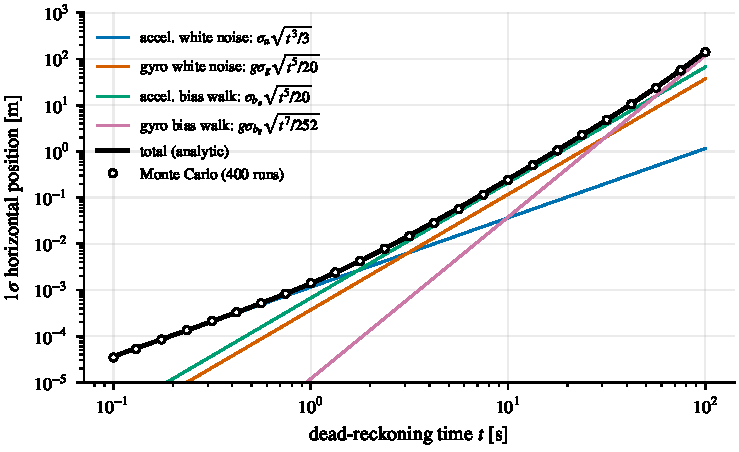
\includegraphics[width=0.88\textwidth]{fig_cov_growth.pdf}
  \caption{Horizontal position standard deviation of a dead-reckoning IMU with EuRoC noise parameters,
  from \eqref{eq:growth-laws}, with a Monte Carlo check (400 runs of the discretized error equations at
  200~Hz). Accelerometer white noise dominates for the first two seconds, the accelerometer bias walk from
  there to about a minute, and then the gyro bias walk takes over with its $t^{7/2}$ growth.}
  \label{fig:cov-growth}
\end{figure}

\begin{proposition}[Dead-reckoning growth laws]
\label{prop:growth-laws}
For a level, stationary IMU with zero initial uncertainty, the horizontal position variance grows as
\begin{equation}
  \sigma_p^2(t) = \underbrace{\frac{\sigma_a^2 t^3}{3}}_{\text{accel.\ white}}
  + \underbrace{\frac{g^2\sigma_g^2 t^5}{20}}_{\text{gyro white}}
  + \underbrace{\frac{\sigma_{b_a}^2 t^5}{20}}_{\text{accel.\ bias walk}}
  + \underbrace{\frac{g^2\sigma_{b_g}^2 t^7}{252}}_{\text{gyro bias walk}} .
  \label{eq:growth-laws}
\end{equation}
\end{proposition}
\begin{proof}
Accelerometer white noise is integrated twice ($m = 2$ in \cref{prop:integrated-noise}). Gyro white noise is integrated
once into tilt, scaled by $g$, and integrated twice more ($m = 3$). The accelerometer bias random walk is
itself integrated white noise, then integrated twice ($m = 3$). The gyro bias random walk adds one more
integration ($m = 4$). The sources are independent, so their variances add.
\end{proof}



\Cref{fig:cov-growth} evaluates \eqref{eq:growth-laws} with EuRoC's parameters. After one second of blind flight the
position uncertainty is about 1~mm, after ten seconds about 25~cm, and after a minute more than 10~m. The
camera's job is to keep the filter permanently in the left part of this plot.

\begin{projectlink}[Milestone 5]
The analytic check of M5 isolates the first term of \eqref{eq:growth-laws}: with $P_0 = 0$, only accelerometer noise and a
fixed orientation, the horizontal position variance must equal $\sigma_a^2t^3/3$. Because $\Phi$ and $Q_d$ are first-order
approximations, the agreement improves as $\Dt\to0$ (\cref{ex:double-integrator-qd}), and the test tolerance should reflect
that.
\end{projectlink}

\paragraph{Why diagonal entries need not grow monotonically.} The attitude covariance is expressed in body axes
(\cref{rem:cov-rotates}). When the vehicle rotates, the attitude block of $\Phi$ rotates the covariance between axes, so an
individual diagonal entry can shrink during pure propagation even though no information is gained. Monotonicity
holds for invariant quantities, such as the eigenvalues of $P_{\theta\theta}$ when the vehicle is not rotating, but not for
individual entries.

% ------------------------------------------------------------------------------
\section{Validating covariance propagation}

Two independent tests catch nearly all propagation bugs.

\paragraph{Finite differences on the discrete propagation.} The Jacobian of one step of the nominal integrator,
computed numerically with $\bplus/\bminus$, must match $\Phi$ column by column (the derivation exercise above). This
catches sign errors, transposes, and blocks placed at wrong indices. The test must use a non-trivial state.

\paragraph{Monte Carlo.} Simulate $M$ noisy IMU sequences from a known trajectory, integrate each with the nominal
equations from a perturbed initial state drawn from $P_0$, and compute the errors
$e^{(j)} = x_{\text{true}}\bminus\hat x^{(j)}$. Their sample covariance must agree with the propagated $P$. If the filter is
correct, the ratio of a sample variance to the predicted variance is distributed as $\chi^2_{M-1}/(M-1)$, so for
$M = 500$ it should lie in $[0.88, 1.13]$ with 95\% probability for each diagonal entry. Larger deviations, or many
entries near the bounds in the same direction, indicate an error in $G_c$, $Q_c$ or the units. This catches errors
that finite differences cannot, such as a wrong noise density or a missing $\Dt$.

\begin{takeaways}
\begin{itemize}
  \item The error state is 15-dimensional with the frozen layout $[\delta p, \delta v, \delta\theta, \delta b_a, \delta b_g]$.
  \item Error dynamics follow from substituting $x = \hat x\bplus\delta x$, subtracting the nominal dynamics, and keeping
        first-order terms. The perturbation convention changes the result.
  \item $\Phi \approx I + F_c\Dt$, $Q_d \approx G_cQ_cG_c\T\Dt$ with continuous densities; clones have identity dynamics.
  \item Position variance grows like $t^3$ (accel.\ noise), $t^5$ (gyro noise, accel.\ bias walk) and $t^7$ (gyro bias walk).
  \item Validate $\Phi$ by finite differences and $P$ by Monte Carlo with statistically justified bounds.
\end{itemize}
\end{takeaways}

\begin{exercises}
  \item Derive the velocity error dynamics for the global perturbation, and compare its structure with your local
        result. Which one depends on the vehicle's heading?
  \item Using your $F_c$, show that $\delta\theta$ is decoupled from $\delta p$ and $\delta v$, and explain this from the cascade structure.
  \item Starting from \eqref{eq:imu-discretization}, write $Q_d$ block by block and check its units.
  \item Implement covariance propagation for the 15-state system in Python and reproduce \cref{fig:cov-growth}, including
        the Monte Carlo points.
  \item For a vehicle rotating about its $z$-axis at 1~rad/s with $P_{\theta\theta} = \diag(10^{-4}, 10^{-6}, 10^{-6})$, propagate
        $P_{\theta\theta}$ for a quarter turn with no noise and observe the diagonal entries.
  \item How large must $M$ be for a Monte Carlo variance check to detect a 10\% error in $\sigma_a$ with high probability?
\end{exercises}


\part{The Error-State Filter in Practice}
\chapter{Measurement Updates, Gating and the Pose Sensor}
\label{ch:updates}
\chaptermark{Measurement Updates} % short running header

\begin{objectives}
\begin{itemize}
  \item Apply the generic manifold update to concrete sensors, deriving $H$ by the elementary Jacobians.
  \item Understand which state directions a measurement observes, from the nullspace of $H$.
  \item Implement the mock pose sensor of Milestone 6 and derive its Jacobian.
  \item Gate measurements with the $\chi^2$ test, and understand how gating fails in an overconfident filter.
  \item Understand how a pose sensor makes velocity and biases observable.
\end{itemize}
\end{objectives}

% ------------------------------------------------------------------------------
\section{The generic update}

\begin{convention}[measurement update, AGENTS.md F3]
\begin{enumerate}
  \item Residual $r = z\bminus h(\hat x)$: plain subtraction for vector measurements; for the pose measurement
        $r = [\,p_{meas} - \hat p;\ \Log_q(\hat q\inv\qprod q_{meas})\,]$.
  \item $H = \partial r/\partial\delta x$ at $\delta x = 0$ using C4 (\cref{sec:manifold-update}), derived by hand and verified by
        finite differences.
  \item $S = HPH\T + R_z$; $K = PH\T S\inv$ by a Cholesky/LDL$^\mathsf{T}$ solve, never an explicit inverse.
  \item Mahalanobis gate $r\T S\inv r < \chi^2_{0.95}(\dim r)$ from a \code{constexpr} table. Rejections are counted and
        logged, never silently dropped.
  \item Joseph form $P \gets (I - KH)P(I - KH)\T + KR_zK\T$, then injection and reset (\cref{sec:reset}).
\end{enumerate}
\end{convention}

Everything specific to a sensor is in $h$ and $H$. The rest of this section derives them for two sensors that the
project does not use, to demonstrate the technique, before turning to the pose sensor it does use.

% ------------------------------------------------------------------------------
\section{Worked example: position with a lever arm}

A GNSS antenna mounted at a known offset $\ell_b$ from the IMU, expressed in the body frame, measures the
antenna position:
\begin{equation}
  z = h(x) + n = p_{wb} + R_{wb}\,\ell_b + n, \qquad n \sim \N(0, \sigma^2I_3).
\end{equation}
The residual is a plain difference, $r = z - (\hat p + \hat R\ell_b)$. To find $H$, perturb the nominal state with
$\bplus$ and expand:
\begin{equation*}
  h(\hat x\bplus\delta x) = \hat p + \delta p + \hat R\Exp(\delta\theta)\ell_b
  \approx \hat p + \delta p + \hat R\ell_b + \hat R\sx{\delta\theta}\ell_b
  = h(\hat x) + \delta p - \hat R\sx{\ell_b}\delta\theta .
\end{equation*}
Reading off the coefficients (the rotation-action row of \cref{tab:jacobians}),
\begin{equation}
  H = \begin{bmatrix} I_3 & 0_3 & -\hat R\sx{\ell_b} & 0_3 & 0_3 \end{bmatrix}.
\end{equation}
The attitude column is non-zero because the antenna swings around the IMU when the body rotates. A
lever-arm position measurement therefore carries attitude information, but only about rotations that move
the antenna: the nullspace of $-\hat R\sx{\ell_b}$ is the direction $\ell_b$, since rotating about the lever arm itself
does not move the antenna.

% ------------------------------------------------------------------------------
\section{Worked example: a direction sensor}

A magnetometer, or an accelerometer used as an inclinometer at rest, measures a known world vector $m_w$ in
body coordinates:
\begin{equation}
  z = R_{wb}\T m_w + n .
\end{equation}
With the inverse-action row of \cref{tab:jacobians}, $h(\hat x\bplus\delta x) = \Exp(-\delta\theta)\hat R\T m_w \approx \hat R\T m_w +
\sx{\hat R\T m_w}\delta\theta$, so
\begin{equation}
  H = \begin{bmatrix} 0_3 & 0_3 & \sx{\hat R\T m_w} & 0_3 & 0_3 \end{bmatrix}.
\end{equation}
$\sx{v}$ has rank two and nullspace $\mathrm{span}(v)$, so a direction measurement observes two of the three attitude
degrees of freedom. The rotation about the measured direction is unobservable. For gravity this is the
familiar statement that an accelerometer at rest gives roll and pitch but not yaw.

\begin{keyidea}[the nullspace of $H$ tells you what a sensor cannot see]
Any error direction $\delta x \in \nullsp(H)$ produces no change in the predicted measurement, so the update cannot
correct it. Reading the nullspace of each new $H$ is a quick sanity check of both the derivation and your
intuition about the sensor.
\end{keyidea}

% ------------------------------------------------------------------------------
\section{The pose sensor of Milestone 6}

Before introducing a camera, the project tests the whole ESKF with a ``mock sensor'' that measures the pose
directly. Ground-truth poses, decimated to about 10~Hz, are corrupted with synthetic noise of known statistics.

\begin{convention}[pose measurement, AGENTS.md C6]
\begin{equation}
  p_{meas} = p_{wb} + n_p, \qquad q_{meas} = q_{wb}\qprod\Exp_q(n_\theta), \qquad
  R_z = \diag(\sigma_p^2 I_3,\ \sigma_\theta^2 I_3).
\end{equation}
\end{convention}

The attitude noise is applied on the right, in the body frame, which is exactly the local perturbation. That
choice makes the residual \eqref{eq:manifold-residual} statistically clean: if the nominal state were exact, the
attitude residual would be exactly $n_\theta$. To generate the noise, draw $n_p$ and $n_\theta$ from seeded
\code{std::mt19937\_64} generators (AGENTS.md E5) with the same $\sigma_p$, $\sigma_\theta$ that appear in $R_z$.

\begin{derivex}{the pose measurement Jacobian $H \in \R^{6\times15}$}{sol:Hpose}
Using \eqref{eq:manifold-H}, derive $H$ for $h(x) = (p_{wb}, q_{wb})$ with the residual of AGENTS.md F3.
\begin{enumerate}
  \item The position rows are a plain difference. Which state blocks does $\hat p + \delta p$ depend on?
  \item For the attitude rows, evaluate $\Log_q\big(\hat q\inv\qprod(\hat q\qprod\Exp_q(\delta\theta))\big)$ and simplify.
        Which elementary Jacobian applies if you instead linearize around a non-zero residual?
  \item Write $H$ in the frozen column order and state its nullspace. Which states are \emph{not} directly measured,
        and how can they still be corrected?
\end{enumerate}
\textbf{Check:} the finite-difference test of $r(\delta x) = h(\hat x\bplus\delta x)\bminus h(\hat x)$ at a non-trivial state, as
required by Milestone 6.
\end{derivex}

\paragraph{How unmeasured states get corrected.} The pose sensor measures neither velocity nor biases, yet the
update corrects both. The mechanism is the cross-covariance built up by propagation. Between updates, a velocity
error produces a growing position error, so $P_{pv}$ becomes large; an accelerometer bias produces a velocity error
and then a position error, so $P_{p b_a}$ grows; a gyro bias produces an attitude error, so $P_{\theta b_g}$ grows. The gain
$K = PH\T S\inv$ has non-zero rows for every state correlated with the measured ones, so each pose update corrects
them in proportion to those correlations.

\paragraph{Why the biases converge.} Observability here has an intuitive reading. The gyro bias is the slope of the
difference between the integrated gyro and the measured attitude, which a sequence of attitude measurements reveals.
The velocity is the slope of the measured position. The accelerometer bias is the difference between the
acceleration implied by successive velocities and the specific force rotated with the (measured) attitude, so it
too becomes observable. Even at rest it is separable from tilt, because the attitude is measured directly. With
pose measurements every state of the IMU error state is observable, and their covariances converge.

% ------------------------------------------------------------------------------
\section{Gating}
\label{sec:gating}

Real measurements include outliers: a misassociated feature, a reflection, a moving object. A single outlier with a
large residual can drag the estimate far away and corrupt the covariance. The $\chi^2$ test of \cref{prop:innovation}
rejects measurements that are statistically implausible given the filter's own uncertainty:
\begin{equation}
  \gamma = r\T S\inv r \ \stackrel{?}{<}\ \chi^2_{1-\alpha}(\dim r).
\end{equation}

\begin{table}[h]
\centering\small
\begin{tabular}{@{}c c c c c c c@{}}
\toprule
$\dim r$ & 1 & 2 & 3 & 4 & 5 & 6 \\
\midrule
$\chi^2_{0.95}$ & 3.841 & 5.991 & 7.815 & 9.488 & 11.070 & 12.592 \\
$\chi^2_{0.99}$ & 6.635 & 9.210 & 11.345 & 13.277 & 15.086 & 16.812 \\
\bottomrule
\end{tabular}
\caption{Gate thresholds. A longer table, up to 600 degrees of freedom, is in \cref{app:tables}.}
\label{tab:chi2-short}
\end{table}

With a 95\% gate, a consistent filter rejects 5\% of perfectly good measurements. That is the price of rejecting
most outliers, and it is why rejections are counted and logged: a rejection rate close to 5\% is a sign of
health, a rate near zero suggests an underconfident filter (or a gate that is too loose to be useful), and a
rate far above 5\% indicates overconfidence or a model error.

\begin{pitfall}[the death spiral]
Gating assumes the filter is consistent. If $P$ is too small, good measurements produce large $\gamma$ and are
rejected; with no corrections $P$ should grow, but if the model's process noise is also too small it grows slowly
while the true error grows quickly, and more measurements are rejected. The filter then dead-reckons with false
confidence until it diverges. When the rejection rate jumps, suspect overconfidence before suspecting outliers.
\end{pitfall}

The threshold depends on the dimension of $r$. A pose measurement uses $\chi^2_{0.95}(6)$, a single image
observation $\chi^2_{0.95}(2)$, and a projected MSCKF feature residual $\chi^2_{0.95}(2M-3)$, where $M$ is the number of
observations (\cref{ch:msckfupdate}). Because the quantiles grow with the dimension, the table is generated offline
and stored as a \code{constexpr} array, which avoids depending on a statistics library in the core.

% ------------------------------------------------------------------------------
\section{Pseudo-measurements and timing}

\paragraph{Pseudo-measurements.} Knowledge that is not a sensor reading can be fed to the filter as if it were one. The most useful is the \term{zero-velocity
update} (ZUPT): when the vehicle is known to be at rest (detected, for example, from a very small variance of the accelerometer and gyroscope readings over
a window), apply the measurement $z = 0 = v_{wb} + n$ with $H = [0\ \ I_3\ \ 0\ \ 0\ \ 0]$ and a small noise covariance. It stops velocity drift, and through the
correlations it also refines tilt and biases. A ZUPT applied when the vehicle is in fact moving is a large, confident, wrong measurement; the detection must
be conservative. Similar pseudo-measurements express a known constant altitude, a non-holonomic constraint (a car does not slide sideways), or a
known landmark.

\paragraph{Measurement timing.} A measurement taken at time $t_z$ must be applied to the state at $t_z$, after propagating exactly to that time
(\cref{ch:strapdown}). Measurements that arrive \emph{late}, after the filter has already propagated past their timestamp, are a problem for every filter:
either the filter buffers the IMU data and re-propagates from $t_z$, or it uses a stochastic clone of the state at $t_z$ (\cref{ch:cloning}), which is exactly the
MSCKF's approach for camera measurements. On EuRoC, data are processed offline in timestamp order, so late measurements do not occur.

% ------------------------------------------------------------------------------
\section{Testing the update}

\begin{projectlink}[Milestone 6]
The exit criteria test properties that hold for any correct implementation:
\begin{itemize}
  \item $H$ passes the finite-difference test at a non-trivial state;
  \item $P_{prior} - P_{post}$ is positive semi-definite (an update never adds uncertainty);
  \item after injection and reset all quaternions are unit, and a second update with the same $z$ produces a residual
        consistent with the first correction;
  \item as $R_z \to 0$ the posterior pose converges to $z$;
  \item with constant synthetic biases, the bias estimates converge to within their own $3\sigma$;
  \item update, injection and reset do not allocate;
  \item a full MH\_01 run with noisy ground-truth updates neither diverges nor produces NaN, and the $\chi^2$ rejection
        count is logged.
\end{itemize}
\end{projectlink}

The ``second update'' test is subtle and worth understanding. After the first update, the nominal pose has moved
toward $z$ by $K r$, so the second residual should be approximately $(I - HK)r$, which is smaller. If it is instead
larger, or has the opposite sign, the injection used the wrong side of the quaternion product or the wrong sign of
$H$.

\begin{takeaways}
\begin{itemize}
  \item Derive $H$ by perturbing $h(\hat x\bplus\delta x)$, expanding to first order and reading off coefficients.
  \item The nullspace of $H$ lists the error directions a sensor cannot see.
  \item The pose sensor's attitude noise is a local perturbation, matching the residual $\Log_q(\hat q\inv\qprod q_{meas})$.
  \item Unmeasured states are corrected through cross-covariances built up by propagation.
  \item Gate with $\chi^2_{0.95}(\dim r)$, log the rejections, and treat a high rejection rate as a symptom of overconfidence.
\end{itemize}
\end{takeaways}

\begin{exercises}
  \item For the lever-arm example, compute $S$ and $K$ for a state with
        \[ P = \diag(\sigma_p^2I,\ \sigma_v^2I,\ \sigma_\theta^2I,\ \sigma_{b_a}^2I,\ \sigma_{b_g}^2I). \]
        Which components of $\delta\theta$ does the update correct?
  \item Derive $H$ for a range measurement to a known beacon $b_w$: $z = \|p_{wb} - b_w\| + n$. What is its nullspace?
  \item Simulate the death spiral: run a 1D constant-velocity filter with $Q$ underestimated by a factor of 100 and a
        95\% gate. Plot the rejection rate and the error over time.
  \item Show that with a pose measurement of a static vehicle, the horizontal accelerometer bias is observable.
        (Hint: what does the attitude measurement remove from the tilt/bias ambiguity of \cref{ch:strapdown}?)
  \item Prove that $P_{prior} - P_{post} = KSK\T \succeq 0$ for the optimal gain, and explain why this test can fail in floating
        point if the simple covariance update is used.
\end{exercises}
% Solutions to the exercises of Chapter 18.
\begin{solutions}
  \item With $H = [\,I_3\ \ 0\ \ {-\hat R\sx{\ell_b}}\ \ 0\ \ 0\,]$ and the block-diagonal $P$, only the position and attitude blocks contribute:
        \[
          S = \sigma_p^2I + \sigma_\theta^2\hat R\sx{\ell_b}\sx{\ell_b}\T\hat R\T + \sigma^2I = \alpha\,I - \sigma_\theta^2\,(\hat R\ell_b)(\hat R\ell_b)\T,
          \qquad \alpha = \sigma_p^2 + \sigma^2 + \sigma_\theta^2\|\ell_b\|^2,
        \]
        using $\sx{\ell}\sx{\ell}\T = -\sx{\ell}^2 = \|\ell\|^2I - \ell\ell\T$. The gain blocks are $K_p = \sigma_p^2S\inv$, $K_\theta = \sigma_\theta^2(-\hat R\sx{\ell_b})\T S\inv = \sigma_\theta^2\sx{\ell_b}\hat R\T S\inv$,
        and zero for velocity and biases. Since $S\inv(\hat R\ell_b) \propto \hat R\ell_b$ and $\sx{\ell_b}\hat R\T\hat R\ell_b = 0$, the attitude gain simplifies to
        \[
          K_\theta = \frac{\sigma_\theta^2}{\sigma_p^2 + \sigma^2 + \sigma_\theta^2\|\ell_b\|^2}\,\sx{\ell_b}\hat R\T .
        \]
        Its range is the range of $\sx{\ell_b}$: the update corrects only the attitude components perpendicular to the lever arm, never the rotation
        about $\ell_b$ itself, which does not move the antenna. Velocity and biases are not corrected here because this prior has no cross-covariances;
        after some propagation they would be.

  \item With $h(x) = \|p - b_w\|$ and $\hat\rho = \|\hat p - b_w\|$, perturbing $p = \hat p + \delta p$ gives $h \approx \hat\rho + u\T\delta p$ with $u = (\hat p - b_w)/\hat\rho$, so
        \[
          H = [\,u\T\ \ 0\ \ 0\ \ 0\ \ 0\,] \in \R^{1\times15} .
        \]
        Its nullspace is 14-dimensional: the two position directions perpendicular to the line of sight (moving on the sphere around the beacon), and
        all velocity, attitude and bias errors. One range observes one number; position perpendicular to the line of sight becomes observable only
        through several beacons or through motion and the correlations it builds.

  \item Simulate a constant-velocity target (acceleration density $\sqrt{0.5}$, position measurements at 10~Hz with unit variance) and run the
        filter with $Q$ divided by 100 and a $\chi^2_{0.95}(1)$ gate. Typical results, per 30-second window:
        \begin{center}\small
        \begin{tabular}{@{}l l l@{}}
        \toprule
        filter & rejection rate & RMS position error \\
        \midrule
        correct $Q$, gated & 2--8\% & 0.4--0.65~m \\
        $Q/100$, gated & 79\%, then 100\% & 26, 126, 243, \dots, 3246~m \\
        $Q/100$, not gated & 0\% & 0.8--1.7~m \\
        \bottomrule
        \end{tabular}
        \end{center}
        The overconfident filter predicts innovations that are far too small, so good measurements fail the gate; each rejection removes the
        correction the filter needed, the error grows, more measurements are rejected, and within half a minute the filter ignores all data and
        dead-reckons. Its reported $\sigma$ (about 200~m at the end) stays far below its actual error. Without the gate the same mistuned filter is
        merely suboptimal: its error stays bounded. A rejection rate far above the design value is the alarm signal (\cref{sec:gating}).

  \item At rest, the accelerometer measures $\hat R\T(-g_w) + b_a$, and to first order a tilt error and a horizontal bias change this reading in the same way:
        in the velocity error dynamics both enter through the horizontal specific-force error, so from accelerations alone only their combination is
        observable (\cref{ch:strapdown}). With a pose sensor, the position measurements make the velocity error and its rate observable (two
        differentiations, as in \cref{sec:observability-linear}), while the attitude measurement observes $\delta\theta$ directly. The rate of the velocity
        error is (tilt term) $+$ (bias term); with the tilt term known from the attitude measurement, the bias term, and hence the horizontal bias, is
        determined. The vertical bias was observable already (it changes the measured magnitude of gravity, which the position measurements expose),
        and the gyro bias is observable from the drift of the attitude between measurements. With a pose sensor, every IMU state is observable,
        which is why the covariances converge in Milestone 6.

  \item For the optimal gain, $P_{\mathrm{prior}} - P_{\mathrm{post}} = KHP = KSK\T$ (\cref{thm:kf-update}), and $KSK\T \succeq 0$ because it is a congruence of $S \succ 0$
        (\cref{prop:psd}). In floating point the simple update $P_{\mathrm{post}} = (I - KH)P$ is neither symmetric nor guaranteed PSD (Exercise 12.3), and
        $P_{\mathrm{prior}} - P_{\mathrm{post}}$ then has rounding-level asymmetry and can have slightly negative eigenvalues, notably in directions the
        measurement does not observe, where the true difference is exactly zero and the computed one is $\pm u\|P\|$. A test must therefore symmetrize the
        difference and allow a tolerance: $\lambda_{\min}\big(\tfrac12(D + D\T)\big) \ge -c\,u\,\|P\|$ with a small constant $c$. Using the Joseph form and
        symmetrizing after each update makes $P_{\mathrm{post}}$ itself PSD, but the difference still needs the tolerance.
\end{solutions}


\chapter{Consistency and Evaluation}
\label{ch:consistency}

\begin{objectives}
\begin{itemize}
  \item Test whether a filter's covariance tells the truth, with NEES, NIS and $3\sigma$ coverage.
  \item Compute exact statistical bounds for single-run and Monte Carlo tests.
  \item Diagnose over- and under-confidence and tune noise parameters without cheating.
  \item Measure trajectory accuracy with ATE and RPE, using the alignment appropriate for VIO.
\end{itemize}
\end{objectives}

A filter produces two things: an estimate and a covariance. Most evaluations look only at the first. But a
filter with good average accuracy and a covariance that is too small is dangerous: it rejects valid measurements,
it reports false confidence to whatever consumes its output, and it eventually diverges. This chapter is about
checking the second output.

% ------------------------------------------------------------------------------
\section{What consistency means}

Recall from \cref{ch:prob} that a filter reporting $(\hat x_k, P_k)$ is consistent if its error $e_k = x_k\bminus\hat x_k$ has
zero mean and covariance $P_k$. Together with \cref{prop:innovation}, a consistent, correctly modeled filter
satisfies three testable properties:
\begin{enumerate}
  \item estimation errors are compatible with $P_k$ (tested with NEES, needs ground truth);
  \item innovations are compatible with $S_k$ (tested with NIS, needs no ground truth);
  \item innovations are white (tested with autocorrelation, needs no ground truth).
\end{enumerate}
The error must be computed with the manifold difference $\bminus$, using exactly the same convention as the
filter's covariance. Comparing a local-perturbation covariance with a global attitude error, or with an Euler
angle difference, produces meaningless statistics.

% ------------------------------------------------------------------------------
\section{Normalized estimation error squared}

\begin{definition}[NEES]
The normalized estimation error squared at time $k$ is
\begin{equation}
  \epsilon_k = e_k\T P_k\inv e_k, \qquad e_k = x_k\bminus\hat x_k .
\end{equation}
\end{definition}

If the filter is consistent and its errors are Gaussian, $\epsilon_k \sim \chi^2_n$ with $n = \dim e$ by
\cref{thm:mahalanobis-chi2}: its expected value is $n$. A single run gives one sample per time step, which is noisy.
Monte Carlo runs average it out. With $N$ independent runs, the average NEES
$\bar\epsilon_k = \frac1N\sum_{j=1}^N\epsilon_k^{(j)}$ satisfies $N\bar\epsilon_k \sim \chi^2_{Nn}$, so the two-sided 95\% interval is
\begin{equation}
  \left[\ \frac{\chi^2_{0.025}(Nn)}{N},\ \frac{\chi^2_{0.975}(Nn)}{N}\ \right].
  \label{eq:anees-bounds}
\end{equation}
For the 15-state IMU filter with $N = 50$ runs this is $[13.52, 16.56]$; for $N = 100$, $[13.95, 16.09]$.
\Cref{app:tables} lists more. Average NEES above the interval means overconfidence (errors larger than claimed);
below means underconfidence.

\begin{figure}[t]
  \centering
  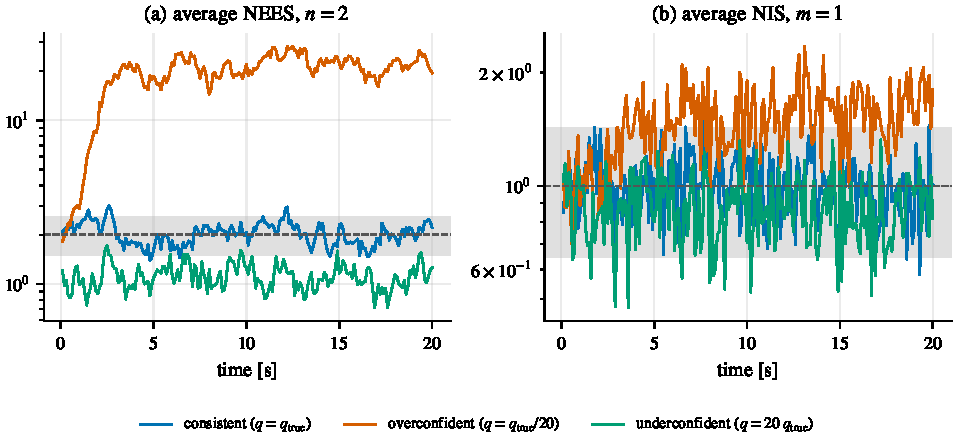
\includegraphics[width=\textwidth]{fig_nees.pdf}
  \caption{Consistency statistics of a constant-velocity filter over 50 Monte Carlo runs, with the 95\%
  acceptance region (gray) of \eqref{eq:anees-bounds}. Underestimating the process noise by a factor of 20 makes the
  filter overconfident: the NEES leaves the region by an order of magnitude, and the NIS rises above it. Overestimating
  it makes the filter underconfident: the NEES falls below the region. Note that the NIS of the underconfident filter
  is less clearly abnormal: NIS alone is a weak detector of underconfidence.}
  \label{fig:nees}
\end{figure}

\paragraph{Block NEES.} The NEES of the full state mixes well-estimated and poorly estimated blocks. Computing it
separately for position, velocity, attitude and biases, each with its own $3\times3$ block of $P$ and $\chi^2_3$ bounds, points
directly at the misbehaving part.

% ------------------------------------------------------------------------------
\section{Normalized innovation squared}

\begin{definition}[NIS]
$\nu_k = r_k\T S_k\inv r_k$, the same quantity the gate computes.
\end{definition}

Under consistency $\nu_k \sim \chi^2_m$ with $m = \dim r_k$. NIS needs no ground truth, so it is the main consistency
monitor on real data. Two summaries are useful: the fraction of updates with $\nu_k$ below its 95\% quantile, which
should be close to 95\% (Milestone 7), and the time-average of $\nu_k$, which should be close to $m$. If measurements have
different dimensions, normalize by $m_k$ or compare each against its own quantile.

\paragraph{$3\sigma$ coverage.} For each scalar component $i$, a consistent Gaussian error lies within $\pm3\sqrt{P_{ii}}$
99.7\% of the time. Plotting errors against their $3\sigma$ envelopes is the most readable diagnostic, and the coverage
fraction is a simple scalar summary. On EuRoC, Milestone 7 requires at least 95\% coverage for velocity and biases.
These states are not measured by the pose sensor, so their consistency is not circular.

% ------------------------------------------------------------------------------
\section{Diagnosing inconsistency}

\begin{table}[t]
\centering\small
\begin{tabularx}{\textwidth}{@{}l l X@{}}
\toprule
\textbf{NEES} & \textbf{NIS} & \textbf{Likely causes} \\
\midrule
high & high & process noise too small; wrong noise units (missing $\Dt$ or $\sqrt{\Dt}$); unmodeled IMU errors; integration error \\
high & normal & errors in directions the measurement does not see (unobservable states, e.g.\ yaw in VIO); wrong $\bminus$ convention in the evaluation \\
normal & high & measurement noise too small; outliers passing the gate; wrong $H$ \\
low & low & process or measurement noise too large \\
high, growing & normal & spurious information along unobservable directions (EKF inconsistency, \cref{ch:observability}) \\
spikes & spikes & time-synchronization errors; wrong extrinsics; bad initialization \\
\bottomrule
\end{tabularx}
\caption{Reading consistency statistics. Combinations narrow the search for the bug.}
\label{tab:consistency-diagnosis}
\end{table}

\Cref{tab:consistency-diagnosis} is a starting point for debugging. Two additional checks are valuable. First, plot each
residual component over time: a non-zero mean reveals a bias (wrong extrinsics, a wrong sign in $h$); slow oscillation
reveals correlated errors (a coloured noise the filter assumes white). Second, compare the covariance with Monte
Carlo statistics on synthetic data, where the truth is known exactly and the noise is exactly as modeled. If the filter
is inconsistent on synthetic data, the bug is in the filter. If it is consistent there but not on real data, the problem is
the model.

\subsection{Tuning without cheating}

\begin{enumerate}
  \item \textbf{Synthetic first.} With synthetic data generated with exactly the filter's noise parameters, there is
        nothing to tune: a consistent implementation must pass. Any failure is a bug.
  \item \textbf{Physically meaningful knobs only.} On real data, adjust the IMU noise densities (start from
        \cref{tab:euroc-imu}, inflate modestly for unmodeled effects) and the measurement noise (start from the pixel
        noise of the detector). Do not add arbitrary noise to arbitrary states.
  \item \textbf{Judge on consistency, not accuracy.} Choose parameters that make NIS and coverage statistics correct.
        Lower trajectory error obtained by making the filter inconsistent will not generalize.
  \item \textbf{Separate tuning from evaluation.} Tune on some sequences and report results on others.
  \item \textbf{Ground truth never enters the filter} except where explicitly allowed and logged (initialization).
\end{enumerate}

% ------------------------------------------------------------------------------
\section{Trajectory accuracy}

Consistency says whether the covariance is honest; accuracy says how small the errors are. VIO accuracy is
reported with two metrics~\cite{sturm2012tum, zhang2018tutorial}.

\subsection{Absolute trajectory error}

The estimated trajectory lives in a world frame that is only defined up to the unobservable directions, so it must
be aligned with the ground truth before comparing. Given time-associated positions $p_i$ (ground truth) and
$\hat p_i$ (estimate), find the transformation that best maps the estimate onto the truth, then compute
\begin{equation}
  \mathrm{ATE}_{\mathrm{RMSE}} = \Big(\frac1N\sum_{i=1}^N\big\|p_i - (R^\star\hat p_i + t^\star)\big\|^2\Big)^{1/2}.
\end{equation}
For rigid alignment, the optimal transformation has a closed form (Kabsch/Umeyama~\cite{umeyama1991}).

\begin{proposition}[Optimal rigid alignment]
\label{prop:umeyama}\label{sec:umeyama}
\index{Umeyama alignment}
Let $\mu$ and $\hat\mu$ be the means of the two point sets, $a_i = p_i - \mu$ and $b_i = \hat p_i - \hat\mu$ the centered points, and
$\Sigma_{ab} = \frac1N\sum_ia_ib_i\T = UDV\T$ an SVD. The minimizer of $\sum_i\|p_i - (R\hat p_i + t)\|^2$ over rotations $R$ and translations $t$ is
\begin{equation}
  R^\star = U\diag\big(1, 1, \det(UV\T)\big)V\T, \qquad t^\star = \mu - R^\star\hat\mu .
\end{equation}
\end{proposition}
\begin{proof}
For fixed $R$, the cost is a quadratic in $t$ minimized where its gradient vanishes, $\sum_i(p_i - R\hat p_i - t) = 0$, i.e.\ $t = \mu - R\hat\mu$: the alignment maps
centroid onto centroid. Substituting, the cost becomes $\sum_i\|a_i - Rb_i\|^2 = \sum_i(\|a_i\|^2 + \|b_i\|^2) - 2\sum_ia_i\T Rb_i$, so we must maximize
$\sum_ia_i\T Rb_i = \tr\big(R\sum_ib_ia_i\T\big) = N\tr(R\,VDU\T) = N\tr(D\,Z)$ with $Z = U\T RV$. $Z$ is orthogonal, so its diagonal entries are at most one in
magnitude, and $\tr(DZ) = \sum_id_iZ_{ii} \le \sum_id_i$, with equality for $Z = I$, i.e.\ $R = UV\T$. If $\det(UV\T) = -1$ this is a reflection, not a rotation; the
best rotation then flips the axis with the smallest singular value, $Z = \diag(1, 1, -1)$, which gives the stated formula.
\end{proof}

If the scale is also free (a similarity transform, needed for monocular vision without an IMU), the optimal scale is
$s^\star = \tr(D\,\diag(1, 1, \det(UV\T)))\big/\frac1N\sum_i\|b_i\|^2$, applied as $s^\star R^\star\hat p_i + t^\star$ with $t^\star = \mu - s^\star R^\star\hat\mu$.

\begin{keyidea}[align only what is unobservable]
Which transformation to allow depends on the estimator. Monocular vision alone has a free scale, so it uses a
similarity transform (7 DOF). VIO has metric scale and observable roll and pitch: its unobservable directions are
exactly translation and yaw. The appropriate alignment is therefore 4-DOF (translation plus a rotation about
gravity)~\cite{zhang2018tutorial}. A full 6-DOF alignment would also remove roll and pitch errors that the
estimator was responsible for.
\end{keyidea}

The 4-DOF alignment follows the same proof with $R$ restricted to rotations $R_z(\psi)$ about the vertical. For centered points $a = (x, y, z)$ (truth)
and $b = (\hat x, \hat y, \hat z)$ (estimate), $a\T R_z(\psi)b = (x\hat x + y\hat y)\cos\psi + (y\hat x - x\hat y)\sin\psi + z\hat z$, whose sum over the points is maximized by
\begin{equation}
  \psi^\star = \atantwo\Big(\sum_i(y_i\hat x_i - x_i\hat y_i),\ \sum_i(x_i\hat x_i + y_i\hat y_i)\Big),
  \label{eq:4dof-yaw}
\end{equation}
again with $t^\star = \mu - R_z(\psi^\star)\hat\mu$.

Milestone 10b reports ATE after SE(3) alignment, as in most published benchmarks; reporting the 4-DOF result
alongside it is more faithful to what VIO can know.

\subsection{Relative pose error}

ATE is dominated by the largest drift and depends on trajectory length and shape. The relative pose error (RPE)
compares relative motions over a fixed distance or time $\Delta$:
\begin{equation}
  E_i = \big(T_{i}\inv T_{i+\Delta}\big)\inv\big(\hat T_i\inv\hat T_{i+\Delta}\big),
\end{equation}
and reports statistics of the translation and rotation parts of $E_i$, often as a percentage of distance traveled. It
needs no global alignment and measures local drift, which is what odometry is about. The \code{evo}
package~\cite{grupp2017evo} computes both metrics with all the alignment variants.

\begin{projectlink}[Milestone 7]
M7 logs $\hat x$, $\diag(P)$, ground truth, NIS and NEES to a preallocated buffer, flushes it outside the hot loop, and
plots $3\sigma$ envelopes and NEES/NIS against their $\chi^2$ bounds from a single script. Exit criteria: average NEES inside
the 95\% interval for 15 DOF over most of a $\geq50$-run synthetic Monte Carlo; NIS within its per-update bound for about
95\% of updates; at least 95\% $3\sigma$ coverage of velocity and biases on MH\_01; zero allocations while logging.
\end{projectlink}

\begin{takeaways}
\begin{itemize}
  \item A filter must be judged on the honesty of its covariance as well as its accuracy.
  \item NEES needs ground truth and tests $P$; NIS needs none and tests $S$. Both are $\chi^2$ under consistency.
  \item Monte Carlo averages have exact bounds $[\chi^2_{0.025}(Nn), \chi^2_{0.975}(Nn)]/N$.
  \item Overconfidence (NEES too high) is the dangerous failure; NIS alone detects underconfidence poorly.
  \item Tune physically meaningful parameters for consistency, on synthetic data first.
  \item Report ATE after an alignment matched to the unobservable directions, and RPE for local drift.
\end{itemize}
\end{takeaways}

\begin{exercises}
  \item Show that the single-run NEES of a consistent 15-state filter exceeds its 95\% quantile 5\% of the time. Why
        is the Monte Carlo average a much sharper test?
  \item Reproduce \cref{fig:nees}. Then make only the measurement noise wrong instead of the process noise and compare
        the signatures.
  \item Derive the closed-form 4-DOF alignment above by maximizing $\sum_i p_i\T R_z(\psi)\hat p_i$ over $\psi$.
  \item Explain why the NEES of yaw in a VIO run on real data tends to grow over time even when the NIS looks
        healthy. (Revisit after \cref{ch:observability}.)
  \item Compute the RPE over 10~m segments for a trajectory with a constant yaw drift of $1^\circ$ per minute flying at
        1~m/s. How does it compare with the ATE after a 10-minute flight?
\end{exercises}
% Solutions to the exercises of Chapter 19.
\begin{solutions}
  \item If the filter is consistent and its errors Gaussian, $\epsilon_k = e_k\T P_k\inv e_k \sim \chi^2_{15}$ (\cref{thm:mahalanobis-chi2}). The 95\% quantile $\chi^2_{0.95}(15) = 25.0$ is
        by definition the value exceeded with probability 5\%, so a single run exceeds it at 5\% of its time steps. A single sample is a weak test:
        its two-sided 95\% range is $[6.3, 27.5]$, a factor of more than four, and a filter whose covariance is too small by 30\% still produces values
        inside it most of the time. Averaging over $N$ independent runs shrinks the spread: $N\bar\epsilon \sim \chi^2_{15N}$ has relative standard deviation
        $\sqrt{2/(15N)}$, and for $N = 50$ the interval is $[13.5, 16.6]$, about $\pm10\%$. A 30\% error now moves the average far outside it.

  \item In a simulation of the same kind as \cref{fig:nees} ($q = r = 1$, 50 runs of 200 steps), the average NEES ($n = 2$) and NIS ($m = 1$) after the
        transient are:
        \begin{center}\small
        \begin{tabular}{@{}l c c@{}}
        \toprule
        filter & NEES (band $[1.48, 2.59]$) & NIS (band $[0.65, 1.43]$) \\
        \midrule
        consistent & 1.9 & 1.00 \\
        $Q/20$ & 20.0 & 1.5 \\
        $20\,Q$ & 1.1 & 0.87 \\
        $R/20$ & 21.7 & 17.5 \\
        $20\,R$ & 1.0 & 0.08 \\
        \bottomrule
        \end{tabular}
        \end{center}
        Both kinds of error make the filter over- or underconfident in the NEES, but the NIS separates them. A wrong measurement noise enters $S$
        directly, so the NIS is wildly off ($17.5$ and $0.08$). A wrong process noise affects $S$ only through $HP^-H\T$, which the measurement noise partly
        masks, so the NIS moves much less ($1.5$ and $0.87$, the latter inside the band). Rule of thumb: NIS problems point at $R$ (or at outliers and
        wrong measurement models), NEES problems with a healthy NIS point at $Q$ or at unobservable directions (\cref{tab:consistency-diagnosis}).

  \item With centered points $a_i = (x_i, y_i, z_i)$ (truth) and $b_i = (\hat x_i, \hat y_i, \hat z_i)$ (estimate),
        \[
          \sum_ia_i\T R_z(\psi)b_i = \cos\psi\underbrace{\sum_i(x_i\hat x_i + y_i\hat y_i)}_{A} + \sin\psi\underbrace{\sum_i(y_i\hat x_i - x_i\hat y_i)}_{B} + \sum_iz_i\hat z_i .
        \]
        As a function of $\psi$ this is $\sqrt{A^2 + B^2}\cos(\psi - \psi_0) + \text{const}$ with $(\cos\psi_0, \sin\psi_0) \propto (A, B)$, so it is maximized at
        $\psi^\star = \atantwo(B, A)$, which is \eqref{eq:4dof-yaw}. (Setting the derivative $-A\sin\psi + B\cos\psi$
        to zero gives $\tan\psi = B/A$, which has two solutions; the $\atantwo$ picks the maximum rather than the minimum.) The translation follows
        as before: $t^\star = \mu - R_z(\psi^\star)\hat\mu$, which maps centroid onto centroid.

  \item The standard EKF linearizes at estimates that change over time, which makes the global yaw appear observable in its linearized model
        (\cref{ch:observability}). The filter then extracts spurious yaw information from measurements that contain none: its yaw variance shrinks,
        or grows more slowly than the true yaw error, which in VIO drifts like a random walk because nothing measures it. The NEES of yaw,
        $e_\psi^2/\sigma_\psi^2$, therefore grows steadily. The NIS stays healthy because innovations depend only on observable quantities (relative motion,
        roll, pitch, scale): an error along an unobservable direction changes no predicted measurement, so it cannot show up in the residuals
        (\cref{tab:consistency-diagnosis}, ``high, growing / normal'').

  \item A yaw drift of $1^\circ$ per minute is $\omega_d = 2.9\times10^{-4}$~rad/s. A 10~m segment takes 10~s at 1~m/s, during which the heading drifts by
        $0.167^\circ$: that is the rotational RPE. The translational RPE is the lateral offset accumulated within the segment, about
        $\tfrac12\omega_dv\,\Delta t^2 = 1.5$~cm (a simulation gives $1.4$~cm), i.e.\ $0.15\%$ of the distance travelled, and it is the same for every segment of the
        flight. For a straight 10-minute flight, by contrast, the estimated path bends into an arc of radius $v/\omega_d = 3.4$~km: the final position error is
        $\tfrac12\omega_dvT^2 = 52$~m, the RMS error without alignment 23~m, and after the best rigid alignment still $3.9$~m. The ATE grows quadratically
        with the duration and depends on the trajectory and on the alignment; the RPE does not grow and measures the drift rate itself, which is why
        odometry is compared with RPE and full trajectories with ATE.
\end{solutions}



\part{Computer Vision}
\chapter{Image Formation and Camera Models}
\label{ch:camera}
\chaptermark{Image Formation} % short running header

\begin{objectives}
\begin{itemize}
  \item Understand how a camera forms an image: pinholes, lenses, focus, sensors, exposure and shutters.
  \item Derive the pinhole projection, the intrinsic matrix and normalized image coordinates.
  \item Use homogeneous coordinates and the basic projective geometry of points, lines and homographies.
  \item Model and invert the radial-tangential lens distortion used by EuRoC, and know the fisheye alternative.
  \item Understand how cameras are calibrated.
  \item State the project's camera measurement model with its noise, derive the projection Jacobian, and understand extrinsics and time offsets.
\end{itemize}
\end{objectives}

% ==============================================================================
\section{How a camera forms an image}

\subsection{From pinhole to lens}

A camera measures the \emph{directions} of light rays. In a \emph{camera obscura}, light from the scene enters a dark box through a tiny hole and
forms an inverted image on the opposite wall: every point of the wall receives light only from the scene point on the straight line through the
hole. This is the \term{pinhole model}, and it is geometrically perfect. It is also impractical: a hole small enough to give a sharp image lets in
very little light.

A lens gathers light through a large aperture and bends it so that all rays from one scene point converge again at one image point. For an ideal
\emph{thin lens} of focal length $f_L$, a point at distance $z_o$ in front of the lens is imaged sharply at distance $z_i$ behind it, where
\begin{equation}
  \frac1{f_L} = \frac1{z_o} + \frac1{z_i} .
\end{equation}
For distant scenes ($z_o \gg f_L$) the image forms at $z_i \approx f_L$, which is where the sensor sits in a camera focused at infinity. Points at other
distances form slightly blurred spots; the range of distances that stays acceptably sharp is the \emph{depth of field}, larger for small apertures and
short focal lengths. The central ray through the lens center is not bent, so the geometry of a focused lens camera is exactly that of a pinhole at
the lens center: the pinhole model describes it, and lens imperfections are added as \emph{distortion} (\cref{sec:distortion}).

\subsection{The image sensor}

The sensor is a grid of light-sensitive \emph{pixels}. Each accumulates charge in proportion to the light it receives during the \emph{exposure time},
and the charge is converted into a number, typically 8 bits per pixel for the monochrome cameras of EuRoC. Several properties of the sensor matter to an
estimator.
\begin{itemize}
  \item \emph{Exposure and motion blur.} A camera rotating at $\omega$ rad/s during an exposure of $T$ seconds smears each point over about $f\omega T$ pixels, with
        $f$ the focal length in pixels. At 1~rad/s, 5~ms and $f = 458$~px this is 2.3~px, enough to degrade feature tracking. EuRoC's difficult
        sequences contain exactly such blur.
  \item \emph{Global versus rolling shutter.} A global shutter exposes all pixels at the same instant, as EuRoC's cameras do. A rolling shutter (common in
        phones) exposes rows one after another, so each row is captured at a different time and, on a moving camera, from a different pose. Rolling-shutter
        images need an extended measurement model.
  \item \emph{Noise and dynamic range.} Pixel values carry photon and electronic noise, and scenes brighter or darker than the sensor's range saturate. Auto
        exposure changes the brightness of the same scene point between frames, which matters for intensity-based tracking (\cref{ch:frontend}).
\end{itemize}

\paragraph{Pixel coordinates.} We write pixel coordinates as $(u, v)$, with $u$ increasing to the right and $v$ increasing downward, and the origin at the
top-left of the image. In OpenCV's convention, integer coordinates are pixel \emph{centers}. The camera frame $C$ is aligned with this: $x_c$ to the right, $y_c$
down, $z_c$ along the optical axis into the scene.

% ==============================================================================
\section{The pinhole projection}

An ideal pinhole camera lets light through a single point, the optical center. A scene point with camera-frame coordinates $p_c = (X, Y, Z)$, with $Z$ along the
optical axis, projects through the center onto an image plane. Placing a virtual image plane at unit distance \emph{in front of} the center (which avoids
the inversion of the physical image) and using similar triangles, the image of the point is
\begin{equation}
  \pi(p_c) = \begin{bmatrix} x \\ y \end{bmatrix} = \begin{bmatrix} X/Z \\ Y/Z \end{bmatrix}.
  \label{eq:pinhole}
\end{equation}
These are the \term{normalized image coordinates}: dimensionless, independent of the lens, and equal to the tangents of the ray's angles from the optical axis.
The vector $\bar x = (x, y, 1)$ is the \term{bearing} of the point, defined up to scale.

\begin{figure}[t]
\centering
\begin{tikzpicture}[scale=1.0]
  \coordinate (O) at (0,0);
  \draw[frameaxis, plotblue] (O) -- (6.2,0) node[right] {$z_c$ (optical axis)};
  \draw[frameaxis, plotorange] (O) -- (0,-1.6) node[below] {$y_c$};
  \fill (O) circle (1.6pt) node[above left] {$C$};
  \draw[thick, primary] (2,1.8) -- (2,-1.4);
  \node[primary, font=\footnotesize, align=center] at (2,2.15) {normalized plane $Z = 1$};
  \coordinate (P) at (5.6,-1.25);
  \fill[plotgreen] (P) circle (2pt) node[right] {$p_c = (X, Y, Z)$};
  \draw[plotgreen, dashed] (O) -- (P);
  \coordinate (I) at (2,{-1.25*2/5.6});
  \fill[conv] (I) circle (1.8pt);
  \node[conv, font=\footnotesize, right] at (2.05,-0.18) {$y = Y/Z$};
  \draw[<->, black!60] (0,0.5) -- (2,0.5) node[midway, above, font=\footnotesize] {$1$};
  \draw[<->, black!60] (0,0.95) -- (5.6,0.95) node[midway, above, font=\footnotesize] {$Z$};
\end{tikzpicture}
\caption{Pinhole projection in the $y$-$z$ plane. The ray from the optical center $C$ to the point intersects the plane $Z = 1$ at height $Y/Z$. All points
along the ray project to the same image point, so depth is lost.}
\label{fig:pinhole}
\end{figure}

\subsection{Intrinsic parameters}

Pixels are obtained by scaling and shifting the normalized coordinates with the \term{intrinsic matrix}:
\begin{equation}
  \begin{bmatrix} u \\ v \\ 1 \end{bmatrix} = K\begin{bmatrix} x \\ y \\ 1 \end{bmatrix}, \qquad
  K = \begin{bmatrix} f_u & s & c_u \\ 0 & f_v & c_v \\ 0 & 0 & 1 \end{bmatrix},
\end{equation}
with focal lengths $f_u, f_v$ in pixels, principal point $(c_u, c_v)$ (where the optical axis pierces the image), and skew $s$ (zero for modern sensors). The
focal length in pixels is the physical focal length divided by the pixel pitch; $f_u \neq f_v$ if pixels are not square. Inverting $K$ turns a pixel into a bearing,
$\bar x = K\inv(u, v, 1)\T$. The horizontal \emph{field of view} of a $W$-pixel-wide image is $2\arctan\big(W/(2f_u)\big)$, ignoring distortion. EuRoC's \code{cam0} has
$f_u = 458.654$, $f_v = 457.296$, $c_u = 367.215$, $c_v = 248.375$ on a $752\times480$ sensor: a horizontal field of view of about $79^\circ$.

% ==============================================================================
\section{Homogeneous coordinates and projective geometry}
\label{sec:homogeneous}

\subsection{Points and lines in the image}

\index{homogeneous coordinates}
The image point $(x, y)$ corresponds to the whole ray of 3D vectors $\lambda(x, y, 1)$, $\lambda \ne 0$. \term{Homogeneous coordinates} make this explicit: a point of the
plane is represented by any non-zero 3-vector $\tilde x = (x_1, x_2, x_3)$, with $\tilde x$ and $\lambda\tilde x$ representing the same point, and the ordinary coordinates
are recovered as $(x_1/x_3, x_2/x_3)$. Vectors with $x_3 = 0$ represent \emph{points at infinity}: directions, where parallel lines meet.

A line $ax + by + c = 0$ is represented by the 3-vector $l = (a, b, c)$, also up to scale, and a point lies on it exactly when
\begin{equation}
  l\T\tilde x = 0 .
\end{equation}
This symmetric relation makes two constructions one-liners:
\begin{itemize}
  \item the line through two points is $l = \tilde x_1\times\tilde x_2$ (it is orthogonal to both, so both lie on it);
  \item the intersection of two lines is $\tilde x = l_1\times l_2$ (by the same argument).
\end{itemize}
Two parallel lines $(a, b, c_1)$ and $(a, b, c_2)$ intersect at $(b, -a, 0)$ times a constant: a point at infinity in their common direction. In an image of a
3D scene, parallel 3D lines are generally not parallel in the image and meet at a finite \emph{vanishing point}, the image of their common direction.

\subsection{Homographies}

\begin{definition}[Homography]
\index{homography}
A \term{homography} (projective transformation) of the plane is a map $\tilde x \mapsto H\tilde x$ for an invertible $3\times3$ matrix $H$, defined up to scale (eight
degrees of freedom).
\end{definition}

Homographies map lines to lines (if $l\T\tilde x = 0$ then $(H\mT l)\T(H\tilde x) = 0$) but do not preserve parallelism, lengths or angles. Two situations in
which they arise are central to vision:
\begin{itemize}
  \item the images of a \emph{plane} in two views are related by a homography (\cref{ch:multiview}), which is the basis of camera calibration below;
  \item two images taken by a camera that only \emph{rotates} are related by the homography $KRK\inv$, independently of the scene (\cref{ch:multiview,ch:frontend}).
\end{itemize}

\subsection{The projection matrix}

In homogeneous coordinates the complete projection of a world point $p_w$ (with homogeneous coordinates $\tilde p_w = (p_w, 1)$) into pixels is a single linear map,
\begin{equation}
  \lambda\begin{bmatrix} u \\ v \\ 1\end{bmatrix} = K\begin{bmatrix} R_{cw} & p_{cw}\end{bmatrix}\tilde p_w = P\,\tilde p_w,
  \qquad P = K\,[R_{cw}\ \ p_{cw}] \in \R^{3\times4},
\end{equation}
where $(R_{cw}, p_{cw})$ maps world coordinates into the camera frame and $\lambda = Z$ is the depth. The \emph{camera matrix} $P$ has eleven degrees of freedom (twelve
entries up to scale): five intrinsic and six extrinsic. Linear methods that estimate $P$, $H$ or the essential matrix from correspondences
(\cref{ch:multiview}) all exploit the fact that projection is linear in homogeneous coordinates.

% ==============================================================================
\section{Lens distortion}
\label{sec:distortion}

Real lenses bend rays, most strongly near the image edges, so the image of a straight line is curved. The \term{radial-tangential} (Brown--Conrady) model
used by EuRoC maps ideal normalized coordinates $(x, y)$ to distorted ones $(x_d, y_d)$:
\begin{align}
  x_d &= x\,(1 + k_1r^2 + k_2r^4) + 2p_1xy + p_2(r^2 + 2x^2), \\
  y_d &= y\,(1 + k_1r^2 + k_2r^4) + p_1(r^2 + 2y^2) + 2p_2xy, \qquad r^2 = x^2 + y^2,
\end{align}
after which $K$ is applied to $(x_d, y_d)$. The \emph{radial} terms ($k_1, k_2$) model the dominant symmetric distortion of a lens; the \emph{tangential} terms ($p_1, p_2$)
model a lens slightly tilted or decentered relative to the sensor. For \code{cam0}, $(k_1, k_2, p_1, p_2) = (-0.2834, 0.07396, 1.94\times10^{-4}, 1.76\times10^{-5})$. The negative
$k_1$ produces \emph{barrel} distortion (\cref{fig:distortion}). At the middle of the left and right image edges the radial factor $1 + k_1r^2 + k_2r^4$ is about $0.79$,
which moves points by about 100 pixels; at the corners it is about $0.73$, a shift of about 160 pixels. Ignoring distortion is therefore not an option.

\begin{figure}[t]
  \centering
  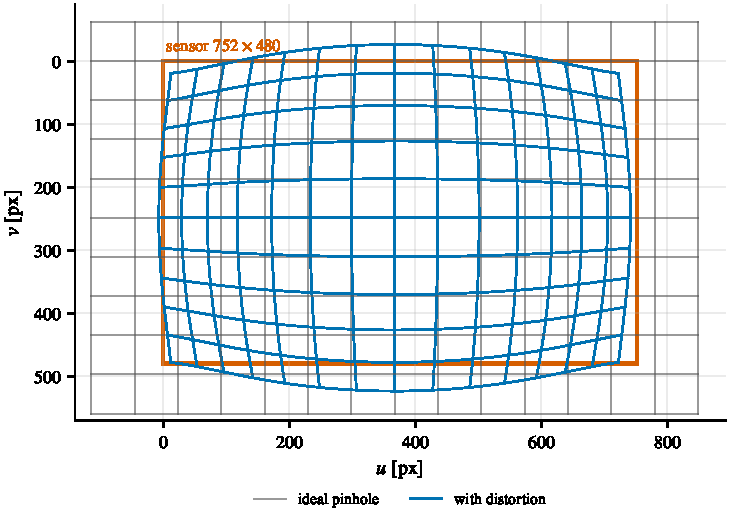
\includegraphics[width=0.84\textwidth]{fig_distortion.pdf}
  \caption{EuRoC \code{cam0} lens distortion. A regular grid in normalized coordinates (gray) is imaged by the real lens as the curved blue grid. Distortion pulls
  points toward the center, increasingly toward the edges, so the sensor (orange) sees a wider field than an ideal pinhole with the same focal length would.}
  \label{fig:distortion}
\end{figure}

\paragraph{Undistortion.} The front end measures distorted pixels and needs ideal normalized coordinates. The model has no closed-form inverse, but a fixed-point
iteration converges quickly for moderate distortion: starting from $x^{(0)} = x_d$,
\begin{equation}
  x^{(j+1)} = \frac{x_d - \Delta_x(x^{(j)}, y^{(j)})}{1 + k_1r_j^2 + k_2r_j^4},\qquad
  y^{(j+1)} = \frac{y_d - \Delta_y(x^{(j)}, y^{(j)})}{1 + k_1r_j^2 + k_2r_j^4},
\end{equation}
where $\Delta$ denotes the tangential terms. A Gauss--Newton iteration (\cref{ch:nlls}) with the $2\times2$ Jacobian of the distortion converges faster and more
reliably near the edges. OpenCV's \code{cv::undistortPoints} implements the iterative scheme. Milestone 8 checks undistortion by distorting and undistorting a
grid of points.

\begin{keyidea}[undistort points, not images]
The estimator needs a few hundred feature locations, not a rectified image. Undistorting only the tracked points costs microseconds; remapping a full image
costs milliseconds, resamples the pixels (blurring them), and changes the noise of the feature detector in a position-dependent way. Track in the raw image and
undistort the tracks.
\end{keyidea}

\paragraph{Wide-angle lenses.} Beyond about $120^\circ$ of field of view, the pinhole model itself breaks down (a ray at $90^\circ$ from the axis would have infinite
normalized coordinates). \emph{Fisheye} models parameterize the image radius as a function of the angle $\vartheta$ of the incoming ray, for example the
equidistant (Kannala--Brandt) model $r_d = \vartheta(1 + k_1\vartheta^2 + k_2\vartheta^4 + \cdots)$. The rest of the pipeline is unchanged: everything downstream of
undistortion works with bearings, which can be represented as unit vectors when they are far from the optical axis.

% ==============================================================================
\section{Camera calibration}

How were EuRoC's intrinsics and distortion coefficients obtained? By observing a known calibration target (a checkerboard or grid of markers) in many
images and fitting the camera model to the observed corner positions.

\paragraph{Zhang's method.} Place the target in the plane $Z = 0$ of its own frame. A target point $(X, Y, 0)$ then projects as
$\lambda\tilde u = K[r_1\ r_2\ r_3\ t](X, Y, 0, 1)\T = K[r_1\ r_2\ t](X, Y, 1)\T$: each image of the target is a homography $H = [h_1\ h_2\ h_3] \propto K[r_1\ r_2\ t]$, estimable from
four or more corner correspondences (\cref{ch:multiview}). Because $r_1$ and $r_2$ are orthonormal, $r_1 = \lambda K\inv h_1$ and $r_2 = \lambda K\inv h_2$ give two
constraints on the matrix $\omega = K\mT K\inv$:
\begin{equation}
  h_1\T\omega h_2 = 0, \qquad h_1\T\omega h_1 = h_2\T\omega h_2 .
\end{equation}
These are linear in the entries of the symmetric $\omega$, so three or more images determine it; $K$ follows from a Cholesky factorization of $\omega$. The linear
estimate is then refined, together with the distortion coefficients and each image's pose, by Levenberg--Marquardt (\cref{ch:nlls}) minimizing the
\emph{reprojection error}, the distance between observed and predicted corners. The residual reprojection error after calibration, typically a few tenths of a
pixel, is the standard measure of calibration quality.

\paragraph{Camera--IMU calibration.} The extrinsics $T_{bc}$ and the time offset are calibrated jointly with the IMU, by moving the rig in front of the target
(\cref{ch:imu}).

% ==============================================================================
\section{The measurement model}

\begin{convention}[camera model, AGENTS.md C6]
In normalized, undistorted image coordinates,
\begin{equation}
  p_c = R_{bc}\T\big(R_{wb}\T(p_f - p_{wb}) - p_{bc}\big), \qquad
  z = \begin{bmatrix} p_{c,x}/p_{c,z} \\ p_{c,y}/p_{c,z} \end{bmatrix} + n_{uv},
  \qquad \sigma_{uv} \approx \sigma_{px}/f .
\end{equation}
\end{convention}

The first equation chains the world-to-body and body-to-camera transformations of \eqref{eq:world-to-camera}. The noise model follows from $u = f_u x + c_u$: a pixel
error $\delta u$ corresponds to a normalized error $\delta u/f_u$. With $\sigma_{px} = 1$~px and $f \approx 458$~px, $\sigma_{uv} \approx 2.2\times10^{-3}$. Strictly, distortion makes the
mapping from pixel noise to normalized noise position-dependent, by the inverse of the distortion Jacobian, and $f_u \neq f_v$. Both effects are small for EuRoC and
conventionally ignored, but they are a legitimate refinement.

% ==============================================================================
\section{The projection Jacobian}

\begin{proposition}[Jacobian of the pinhole projection]
\label{prop:proj-jacobian}
\begin{equation}
  \frac{\partial\pi}{\partial p_c} = \frac{1}{Z}\begin{bmatrix} 1 & 0 & -X/Z \\ 0 & 1 & -Y/Z \end{bmatrix}
  = \frac1Z\begin{bmatrix} I_2 & -\pi(p_c) \end{bmatrix}.
\end{equation}
\end{proposition}
\begin{proof}
Differentiate $X/Z$ and $Y/Z$ with the quotient rule: $\partial(X/Z)/\partial X = 1/Z$, $\partial(X/Z)/\partial Z = -X/Z^2$, and similarly for $Y/Z$.
\end{proof}

The Jacobian has rank two, and its nullspace is spanned by $p_c$ itself: moving the point along its viewing ray does not change its image. This is the single-view
loss of depth in differential form, and it is why a feature must be observed from at least two sufficiently different viewpoints before it constrains anything
(\cref{ch:multiview}). The factor $1/Z$ says that distant points have small image motion for a given change in position. They constrain rotation well and
translation poorly.

The full measurement Jacobian with respect to the filter state is the chain-rule product of this matrix with the Jacobian of $p_c$ with respect to the clone pose
and the feature position. Deriving those is part of \cref{ch:msckfupdate}.

\begin{pitfall}[points behind the camera]
\eqref{eq:pinhole} happily projects points with $Z < 0$, flipping their image through the center. A triangulation or linearization that produces a negative depth must
be rejected (the \emph{cheirality} check), not projected. Points with very small positive $Z$ produce huge Jacobians and should be rejected too.
\end{pitfall}

% ==============================================================================
\section{Extrinsics and time offset}

\paragraph{Extrinsic calibration.} The transformation $T_{bc}$ between the IMU and the camera is estimated offline, for EuRoC with Kalibr~\cite{furgale2013kalibr}, and
stored as \code{T\_BS} in \code{cam0/sensor.yaml}. Its rotation is close to a permutation of axes, and its translation is a few centimeters (\cref{app:euroc}). An error of
$\delta\phi$ in the extrinsic rotation biases every predicted bearing by about $\delta\phi$, which looks to the filter like a systematic residual. A translation error matters
mostly for near points. The project treats $T_{bc}$ as exact (AGENTS.md C3). Estimating it online is a stretch goal.

\paragraph{Time offset.} If the camera timestamp differs from the IMU clock by $t_d$, a feature moving across the image at velocity $\dot z$ is measured with an error of
about $\dot z\,t_d$. A 1~ms offset at an image-plane velocity of 0.5 normalized units per second (fast rotation) is an error of $5\times10^{-4}$, a quarter of a pixel.
EuRoC is hardware synchronized, so $t_d \approx 0$; consumer devices can have offsets of tens of milliseconds and must estimate it online~\cite{li2014timeoffset}.

\begin{takeaways}
\begin{itemize}
  \item A focused lens camera has the geometry of a pinhole at the lens center; lens imperfections are modeled as distortion.
  \item Exposure time causes motion blur of about $f\omega T$ pixels; EuRoC's global shutter exposes all pixels at once.
  \item Normalized coordinates $(X/Z, Y/Z)$ are lens-independent bearings; $K$ maps them to pixels.
  \item Homogeneous coordinates make projection linear; lines through points and intersections of lines are cross products; homographies map planes and pure
        rotations between views.
  \item EuRoC's lens has strong barrel distortion; undistort the tracked points, not the images.
  \item Cameras are calibrated by fitting the model to images of a known target, minimizing reprojection error.
  \item $\partial\pi/\partial p_c = \frac1Z[I_2\ \ {-\pi(p_c)}]$; its nullspace is the viewing ray.
\end{itemize}
\end{takeaways}

\begin{exercises}
  \item A lens with $f_L = 4$~mm is focused at infinity. How far must the sensor move to focus on an object at 0.5~m?
  \item Compute the horizontal and vertical fields of view of \code{cam0} with and without distortion.
  \item Compute the intersection of the lines $x + y = 1$ and $x - y = 0$ with homogeneous coordinates, and the line through $(1, 2)$ and $(3, 1)$.
  \item Show that two parallel lines intersect at a point at infinity, and find the vanishing point of the image of a family of parallel 3D lines with
        direction $d$ under the camera $P = K[I\ \ 0]$.
  \item Implement distortion and fixed-point undistortion for the EuRoC model. How many iterations are needed for $10^{-6}$ accuracy at the image corners? Compare
        with Gauss--Newton.
  \item Derive the two linear constraints of Zhang's method from the orthonormality of $r_1$ and $r_2$.
  \item A point at depth 10~m is observed by a camera translating sideways at 1~m/s and rotating at 1~rad/s. Which motion dominates its image velocity? What does
        this imply for the observability of translation from distant points?
\end{exercises}

\chapter{Digital Image Processing}
\label{ch:imageproc}

\begin{objectives}
\begin{itemize}
  \item Treat an image as a sampled function, and filter it by convolution.
  \item Smooth images with Gaussian kernels, and understand separability and cost.
  \item Compute image gradients robustly with derivative-of-smoothing kernels such as Sobel and Scharr.
  \item Understand why images must be blurred before they are down-sampled, and build Gaussian pyramids.
  \item Interpolate images at sub-pixel positions, find local maxima, and refine them to sub-pixel accuracy.
  \item Know how photometric changes affect intensity-based methods.
\end{itemize}
\end{objectives}

Feature detection and tracking (\cref{ch:frontend}) operate on raw pixel arrays: they smooth them, differentiate them, shrink them and sample them between
pixels. This chapter develops these operations from first principles, as far as the front end needs them.

% ==============================================================================
\section{Images as functions}

A grayscale image is a function $I(u, v)$ giving the brightness at image position $(u, v)$, sampled on the integer grid of pixel centers and quantized,
typically to integers between 0 and 255. In memory it is a 2D array indexed by row and column, $I[\text{row}, \text{col}] = I(u = \text{col}, v = \text{row})$; mixing up the
two orders is a classic bug. Color images have three such channels; a monochrome image can be formed as a weighted sum of them. EuRoC's cameras are
monochrome.

Between pixels, $I$ is undefined until we decide how to interpolate it (\cref{sec:interpolation}). Its derivatives must be approximated by differences of
nearby pixels (\cref{sec:image-derivatives}). Both operations are sensitive to noise and to aliasing, which is what the rest of this chapter is about.

% ==============================================================================
\section{Linear filtering}

\subsection{Correlation and convolution}

\index{convolution}
\termi{Linear filtering}{linear filtering} replaces each pixel by a weighted sum of its neighbors, with the weights given by a small array $h$, the \emph{kernel}. Two closely related
forms exist:
\begin{equation}
\begin{aligned}
  \text{correlation:}&\quad (h\star I)[u, v] = \sum_{i,j}h[i, j]\,I[u + i, v + j], \\
  \text{convolution:}&\quad (h * I)[u, v] = \sum_{i,j}h[i, j]\,I[u - i, v - j] .
\end{aligned}
\end{equation}
Convolution flips the kernel; for symmetric kernels the two coincide. Both are \emph{linear} and \emph{shift-invariant}: filtering a shifted image gives the shifted
filtered image. Convolution is also commutative and associative, so a cascade of filters equals a single filter, $h_2 * (h_1 * I) = (h_2 * h_1) * I$. Near the image
border the kernel extends past the edge, and the missing pixels must be invented: by zeros, by replicating the border, or by reflecting the image. Results
within a kernel radius of the border are always less reliable, which is why detectors ignore a margin there.

A $k\times k$ kernel costs $k^2$ multiplications per pixel. A kernel that factors as an outer product of a column and a row, $h = h_vh_u\T$, is \emph{separable}: filtering
with $h$ equals filtering the rows with $h_u$ and then the columns with $h_v$, at a cost of $2k$ per pixel.

\subsection{Smoothing}

Averaging neighbors reduces noise. The simplest kernel, the \emph{box filter}, averages a $k\times k$ square. The \term{Gaussian filter} weights neighbors by
\begin{equation}
  G_\sigma(u, v) = \frac{1}{2\pi\sigma^2}\exp\!\Big(-\frac{u^2 + v^2}{2\sigma^2}\Big) = g_\sigma(u)\,g_\sigma(v), \qquad g_\sigma(x) = \frac{1}{\sqrt{2\pi}\sigma}e^{-x^2/2\sigma^2},
\end{equation}
sampled at integer offsets, truncated at about $\pm3\sigma$ and renormalized to sum to one. The factorization shows that it is separable. The Gaussian is preferred
over the box because it has no sharp edges: its frequency response is itself a Gaussian, which removes high frequencies smoothly without the ripples of the
box filter. Cascading two Gaussian filters gives a Gaussian whose variances add, $G_{\sigma_1}*G_{\sigma_2} = G_{\sqrt{\sigma_1^2 + \sigma_2^2}}$. Small Gaussians are well
approximated by binomial kernels, $\tfrac14[1, 2, 1]$ and $\tfrac1{16}[1, 4, 6, 4, 1]$ in each direction.

% ==============================================================================
\section{Image derivatives}
\label{sec:image-derivatives}

\index{image gradient}
The \term{image gradient} $\nabla I = (I_u, I_v)$ points in the direction of fastest brightness increase, and its magnitude measures the local contrast. It is
approximated by differences, for example the central difference $I_u[u, v] \approx \tfrac12(I[u + 1, v] - I[u - 1, v])$, a correlation with $\tfrac12[-1, 0, 1]$.

Differentiation amplifies noise: a derivative multiplies each frequency component by its frequency, so pixel-to-pixel noise, the highest frequency present,
is amplified most. The remedy is to smooth before differentiating, and since both are convolutions, to combine them into one kernel. The \emph{Sobel}
operator smooths across the derivative direction with $[1, 2, 1]$ and differentiates along it:
\begin{equation}
  S_u = \begin{bmatrix} 1 \\ 2 \\ 1 \end{bmatrix}\begin{bmatrix} -1 & 0 & 1 \end{bmatrix} = \begin{bmatrix} -1 & 0 & 1 \\ -2 & 0 & 2 \\ -1 & 0 & 1 \end{bmatrix},
  \qquad S_v = S_u\T .
\end{equation}
The \emph{Scharr} operator uses $[3, 10, 3]$ instead of $[1, 2, 1]$, which gives gradient directions that are more accurate for all orientations; OpenCV's
Lucas--Kanade tracker uses it. More generally, the \emph{derivative of a Gaussian}, $\partial G_\sigma/\partial u$, smooths and differentiates at a chosen scale $\sigma$.
Whatever the kernel, it is a weighted difference: its entries sum to zero, so it ignores uniform brightness, and its scale must be divided out when absolute
gradient values matter (Sobel's sum of positive weights is 4 times the step, so $S_u\star I \approx 8I_u$).

\begin{figure}[t]
  \centering
  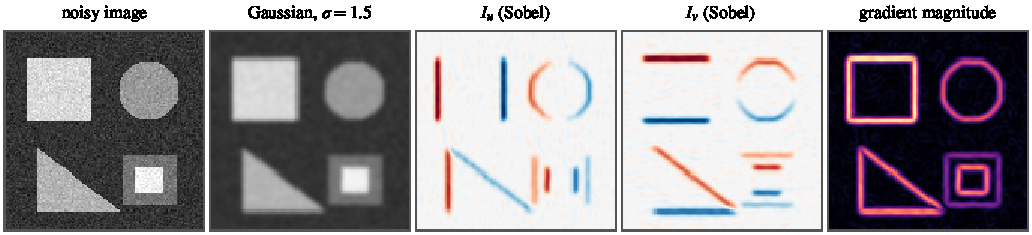
\includegraphics[width=\textwidth]{fig_image_filters.pdf}
  \caption{A synthetic noisy image, its Gaussian smoothing ($\sigma = 1.5$~px), its Sobel derivatives $I_u$ and $I_v$, and the gradient magnitude. Vertical edges respond in
  $I_u$, horizontal edges in $I_v$; corners respond in both, which is what corner detectors look for.}
  \label{fig:image-filters}
\end{figure}

% ==============================================================================
\section{Sampling, aliasing and pyramids}
\label{sec:pyramids}

\subsection{Aliasing in images}

An image is a sampled signal, and the sampling theorem (\cref{ch:processes}) applies in each direction: a pixel grid can represent spatial frequencies up to half a
cycle per pixel. Shrinking an image by keeping every other pixel halves the representable frequency. Any finer detail does not vanish: it \emph{aliases} into false
coarse patterns (moir\'e). The cure is the same as for any sampled signal: low-pass filter, by blurring, before down-sampling.

\begin{figure}[t]
  \centering
  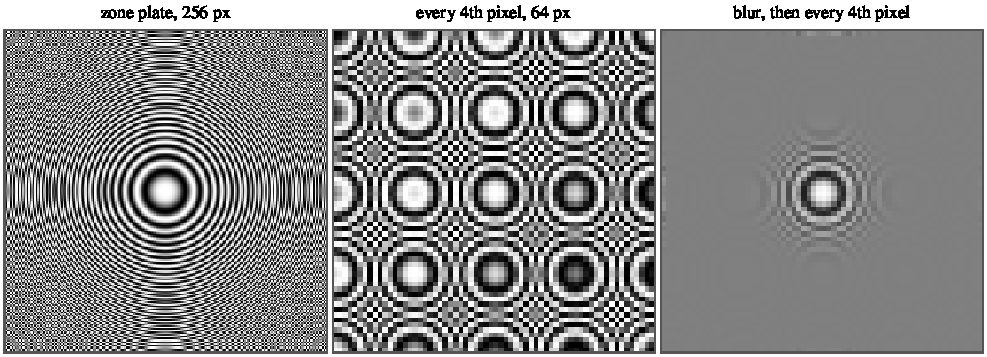
\includegraphics[width=\textwidth]{fig_aliasing_image.pdf}
  \caption{Aliasing in images. A ``zone plate'', whose spatial frequency increases away from the center (left), is shrunk four times by keeping every fourth pixel
  (middle) and by Gaussian blurring first (right). Naive sub-sampling creates false ring patterns; blurring removes the frequencies that cannot be represented.}
  \label{fig:aliasing-image}
\end{figure}

\subsection{Gaussian pyramids}

\index{image pyramid}
A \term{Gaussian pyramid} is a sequence of images, each a blurred and half-resolution copy of the previous one:
\begin{equation}
  I_{\ell+1} = \downarrow_2\big(G * I_\ell\big),
\end{equation}
where $G$ is a small Gaussian (OpenCV's \code{pyrDown} uses the binomial kernel $\tfrac1{16}[1, 4, 6, 4, 1]$ in each direction) and $\downarrow_2$ keeps every second row and
column. Level $\ell$ has $2^{-\ell}$ of the original resolution in each direction, so a pixel position $u_0$ at level 0 corresponds to $u_\ell \approx u_0/2^\ell$ at level $\ell$ (up
to half-pixel conventions). The whole pyramid costs only a third more memory than the original image ($1 + \tfrac14 + \tfrac1{16} + \cdots = \tfrac43$).

\begin{figure}[t]
  \centering
  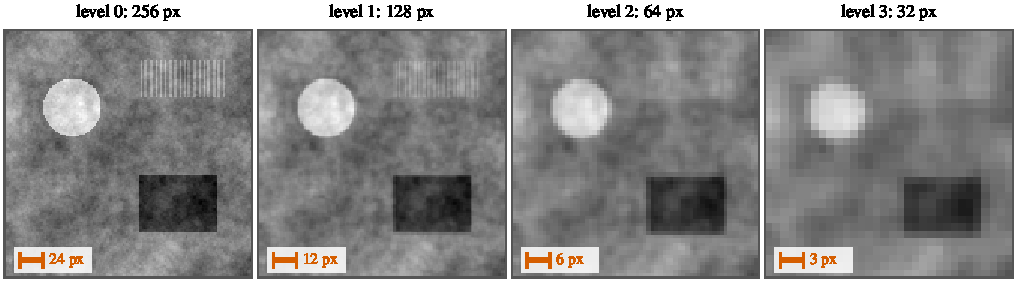
\includegraphics[width=\textwidth]{fig_pyramid.pdf}
  \caption{Four levels of a Gaussian pyramid of a textured synthetic image, displayed at a common size. Fine texture disappears level by level; coarse structure
  survives. A displacement of 24~px at level 0 is a displacement of 3~px at level 3.}
  \label{fig:pyramid-levels}
\end{figure}

Pyramids serve two purposes in the front end. Motion that is large in pixels at full resolution is small at coarse levels, where an iterative tracker can
capture it (\cref{ch:frontend}). And structures of different sizes are best detected at different scales.

% ==============================================================================
\section{Interpolation}
\label{sec:interpolation}

\index{bilinear interpolation}
Sub-pixel tracking needs image values and gradients at non-integer positions. Writing a position as $(u_0 + a, v_0 + b)$ with integer $(u_0, v_0)$ and fractional parts
$a, b \in [0, 1)$:
\begin{itemize}
  \item \emph{nearest neighbor} takes the closest pixel: fast, but the result jumps as the position moves, which ruins sub-pixel accuracy;
  \item \term{bilinear interpolation} interpolates linearly in $u$ along the two neighboring rows and then linearly in $v$ between the results:
  \begin{equation}
    I(u_0 + a, v_0 + b) = (1 - a)(1 - b)\,I_{00} + a(1 - b)\,I_{10} + (1 - a)b\,I_{01} + ab\,I_{11},
  \end{equation}
  with $I_{ij} = I[u_0 + i, v_0 + j]$. The result is continuous, and the weights are the areas of the rectangles opposite each corner;
  \item \emph{bicubic} interpolation fits a smooth cubic patch to a $4\times4$ neighborhood; it has continuous derivatives at the cost of 16 pixels per sample.
\end{itemize}
Lucas--Kanade trackers use bilinear interpolation for both the image and its gradients. With images represented as 8-bit integers, implementations use fixed-point
weights for speed, which limits the attainable sub-pixel resolution to a few hundredths of a pixel, well below the noise of real tracking.

% ==============================================================================
\section{Finding local maxima}

Detectors compute a response map (corner strength, for example) and select the pixels where it is large \emph{and} locally maximal. \termi{Non-maximum suppression}{non-maximum suppression}
keeps a pixel only if its response exceeds a threshold and is the largest in its neighborhood (a $3\times3$ window, or a larger radius to enforce spacing between
detections). The location of a maximum can then be refined below the pixel grid by fitting a parabola through the response $r_{-1}, r_0, r_1$ at the maximum and its two
neighbors in each direction; the vertex lies at the offset
\begin{equation}
  \delta = \frac{r_{-1} - r_{1}}{2\,(r_{-1} - 2r_0 + r_{1})}
\end{equation}
pixels from the center. Sub-pixel accuracy at the detection stage is less important for tracking-based front ends, whose tracker refines positions anyway.

% ==============================================================================
\section{Photometric changes}

Intensity-based methods assume that a scene point keeps its brightness between frames (\cref{ch:frontend}). Auto-exposure, lighting changes and non-Lambertian
surfaces violate this. A common model is an affine change, $I_2 \approx \alpha I_1 + \beta$. Gradients are unaffected by $\beta$, and comparing patches after subtracting their
means and dividing by their standard deviations (\emph{zero-mean normalized cross-correlation}) is unaffected by both. Some trackers estimate $\alpha$ and $\beta$
along with the motion; others pre-process images, for example with histogram equalization, to reduce the variation.

\begin{takeaways}
\begin{itemize}
  \item Filtering is convolution with a kernel; separable kernels cost $2k$ instead of $k^2$ per pixel.
  \item Gaussian smoothing reduces noise without ringing; variances of cascaded Gaussians add.
  \item Derivatives amplify noise; Sobel, Scharr and derivative-of-Gaussian kernels smooth and differentiate at once.
  \item Down-sampling without blurring aliases; a Gaussian pyramid blurs and halves the resolution at each level.
  \item Bilinear interpolation gives continuous sub-pixel samples; non-maximum suppression and parabola fits localize detections.
  \item Normalize patches when brightness may change between frames.
\end{itemize}
\end{takeaways}

\begin{exercises}
  \item Show that the 2D Gaussian kernel is separable, and that filtering with it costs $2k$ operations per pixel for a $k$-tap kernel.
  \item Show that convolving $\tfrac12[1, 1]$ with itself repeatedly produces the binomial kernels, and that their variance grows linearly with the number of
        convolutions.
  \item Compute the response of the Sobel kernel $S_u$ to a linear ramp $I(u, v) = cu$, and explain the factor 8.
  \item Generate a zone plate and reproduce \cref{fig:aliasing-image}. How large must the blur be before shrinking by 4?
  \item Derive the bilinear interpolation formula by interpolating first along $u$ and then along $v$, and show that the result does not depend on the order.
  \item Derive the parabola-vertex formula for sub-pixel peak refinement.
\end{exercises}
% Solutions to the exercises of Chapter 21.
\begin{solutions}
  \item The exponent splits, $e^{-(u^2 + v^2)/2\sigma^2} = e^{-u^2/2\sigma^2}e^{-v^2/2\sigma^2}$, and so does the constant, $\frac1{2\pi\sigma^2} = \frac1{\sqrt{2\pi}\sigma}\cdot\frac1{\sqrt{2\pi}\sigma}$, so
        $G_\sigma(u, v) = g_\sigma(u)g_\sigma(v)$. Sampled on a square $k\times k$ grid the kernel is the outer product $h = gg\T$ of the sampled 1D kernel, and normalizing
        each 1D kernel to unit sum normalizes the product too. Then
        \[
          (h * I)[u, v] = \sum_jg[j]\Big(\sum_ig[i]\,I[u - i, v - j]\Big):
        \]
        the inner sum filters every row with $g$ ($k$ multiplications per pixel) and the outer sum filters the columns of the result ($k$ more), $2k$ in total
        instead of $k^2$. For $\sigma = 1.5$ truncated at $\pm3\sigma$ ($k = 11$) this is 22 instead of 121. Truncating to a \emph{disk} instead of a square would destroy
        the factorization.

  \item The kernel $[a_0, \dots, a_n]$ corresponds to the polynomial $\sum_ia_iz^i$, and convolution of kernels is multiplication of polynomials. Convolving
        $\tfrac12[1, 1]$ with itself $n$ times gives $\big(\tfrac12(1 + z)\big)^n = 2^{-n}\sum_i\binom{n}{i}z^i$: the binomial kernels $\tfrac14[1, 2, 1]$, $\tfrac18[1, 3, 3, 1]$, $\tfrac1{16}[1, 4, 6, 4, 1]$, \dots.
        A non-negative kernel with unit sum is a probability distribution, and the convolution of two distributions is the distribution of the sum of
        independent variables, whose variances add (\cref{ch:prob}). The two-point kernel $\tfrac12[1, 1]$ has variance $\tfrac14$, so the $n$-fold kernel has variance $n/4$:
        $\tfrac12$ for $[1, 2, 1]$, $1$ for $[1, 4, 6, 4, 1]$. By the central limit theorem the binomial kernels approach Gaussians with $\sigma = \sqrt n/2$; OpenCV's
        \code{pyrDown} kernel is a Gaussian with $\sigma = 1$~px.

  \item At pixel $(u, v)$ the correlation sums $S_u[j, i]\,c\,(u + i)$. In each row the weights $-1, 0, 1$ give $c(u + 1) - c(u - 1) = 2c$, and the three rows are
        weighted $1, 2, 1$, so
        \[
          (S_u\star I)[u, v] = (1 + 2 + 1)\cdot2c = 8c,
        \]
        everywhere, for a true derivative $I_u = c$. The factor 8 is the product of the smoothing kernel's sum (4) and the distance between the differenced
        pixels (2). Divide by 8 to obtain the gradient (by 32 for Scharr, whose smoothing kernel sums to 16). With convolution instead of correlation the
        kernel is flipped and the response is $-8c$: check the sign convention of whatever library you use.

  \item A zone plate $I = \tfrac12 + \tfrac12\cos(\pi r^2/n)$ on an $n\times n$ grid (the figure uses $n = 256$) has phase $\pi r^2/n$, hence local frequency $r/n$ cycles per pixel. After
        keeping every fourth pixel the representable limit is $\tfrac18$ cycle per original pixel, so the true rings beyond $r = n/8 = 32$ cannot be represented
        and should become uniform gray; instead, naive sub-sampling folds them into false rings, with new ``centers'' where the frequency is a multiple of the
        new sampling rate $\tfrac14$. A Gaussian blur multiplies frequency $f$ by $e^{-2\pi^2\sigma^2f^2}$. Measuring the false pattern in the region $48 < r < 128$:
        \begin{center}\small
        \begin{tabular}{@{}l c c c c c@{}}
        \toprule
        blur $\sigma$ (px) & 0 & 1 & 1.5 & 2 & 3 \\
        \midrule
        RMS of false pattern & 0.353 & 0.061 & 0.018 & 0.005 & 0.002 \\
        response at $f = \tfrac18$ (kept detail) & 1 & 0.73 & 0.50 & 0.29 & 0.06 \\
        response at $f = \tfrac14$ (aliases to DC) & 1 & 0.29 & 0.06 & 0.007 & $10^{-5}$ \\
        \bottomrule
        \end{tabular}
        \end{center}
        A blur of $\sigma \approx 2$~px, half the shrink factor, removes the aliasing (as in \cref{fig:aliasing-image}); much more also removes detail the smaller image could
        have kept. The same rule, $\sigma \approx s/2$ for a shrink by $s$, gives \code{pyrDown}'s $\sigma = 1$ for $s = 2$.

  \item Along the row $v_0$, linear interpolation gives $(1 - a)I_{00} + aI_{10}$, and along the row $v_0 + 1$, $(1 - a)I_{01} + aI_{11}$. Interpolating these linearly in $v$ with
        weights $1 - b$ and $b$ gives the formula of \cref{sec:interpolation}. In the other order, the columns give $(1 - b)I_{00} + bI_{01}$ and $(1 - b)I_{10} + bI_{11}$, and
        interpolating in $u$ gives $(1 - a)(1 - b)I_{00} + (1 - a)bI_{01} + a(1 - b)I_{10} + abI_{11}$, the same four products. Without expanding: both results have the form
        $c_0 + c_1a + c_2b + c_3ab$ and take the four corner values at the corners, and those four conditions determine the four coefficients uniquely. The
        interpolant is linear along every row and column but quadratic along diagonals, and its derivatives jump at pixel boundaries.

  \item Fit $r(x) = Ax^2 + Bx + C$ through $(-1, r_{-1})$, $(0, r_0)$, $(1, r_1)$: $C = r_0$, $A + B + C = r_1$ and $A - B + C = r_{-1}$, so
        $B = \tfrac12(r_1 - r_{-1})$ and $A = \tfrac12(r_{-1} - 2r_0 + r_1)$. The vertex is at
        \[
          \delta = -\frac{B}{2A} = \frac{r_{-1} - r_1}{2(r_{-1} - 2r_0 + r_1)} .
        \]
        If $r_0$ is the largest of the three, $A < 0$ (a maximum), and $|r_{-1} - r_1| \le (r_0 - r_{-1}) + (r_0 - r_1) = 2|A|$, so $|\delta| \le \tfrac12$: the refined peak stays within
        the pixel. Real peaks are not parabolas, and the fit is biased toward the pixel center: for a Gaussian peak of width $\sigma = 1$~px at a true
        offset of $0.3$~px it returns $0.25$, a bias of up to $0.05$~px, larger for sharper peaks.
\end{solutions}


\chapter{Feature Detection and Tracking}
\label{ch:frontend}

\begin{objectives}
\begin{itemize}
  \item Derive the structure tensor from the auto-correlation of an image patch, and understand corner detectors (Harris, Shi--Tomasi, FAST).
  \item Derive Lucas--Kanade optical flow from brightness constancy, as a Gauss--Newton problem, including the aperture problem.
  \item Implement iterative, pyramidal Lucas--Kanade tracking, and know its failure modes.
  \item Build a robust tracking pipeline: bucketing, forward-backward checks, IMU-aided prediction and geometric verification.
  \item Manage feature tracks through their life cycle with bounded memory.
\end{itemize}
\end{objectives}

The front end turns a stream of images into \emph{feature tracks}: for each tracked scene point, the list of its undistorted normalized coordinates in the images
where it was seen, with the image timestamps. Everything the MSCKF knows about the scene comes from these tracks, so their quality bounds the quality of the
estimator.

\begin{figure}[h]
\centering
\begin{tikzpicture}[node distance=4mm and 5mm, every node/.style={block, font=\footnotesize, minimum width=19mm}]
  \node (img) {image $k$};
  \node (pyr) [right=of img] {build\\pyramid};
  \node (lk) [right=of pyr] {track with\\pyramidal LK};
  \node (fb) [right=of lk] {forward-\\backward check};
  \node (und) [below=of fb] {undistort\\points};
  \node (ran) [left=of und] {RANSAC\\(E or 2-pt)};
  \node (det) [left=of ran] {detect new\\corners (grid)};
  \node (out) [left=of det, fill=white] {tracks to\\estimator};
  \draw[->] (img) -- (pyr); \draw[->] (pyr) -- (lk); \draw[->] (lk) -- (fb);
  \draw[->] (fb) -- (und); \draw[->] (und) -- (ran); \draw[->] (ran) -- (det); \draw[->] (det) -- (out);
\end{tikzpicture}
\caption{A KLT-based front end, as used by MSCKF-style estimators.}
\label{fig:frontend-pipeline}
\end{figure}

% ==============================================================================
\section{What makes a good feature}

\subsection{The auto-correlation of a patch}

A feature is useful if it can be found again, precisely, in the next image. Consider a small window $W$ around a point and ask how much the window changes when
shifted by a small displacement $d$. Measure the change by the weighted sum of squared differences
\begin{equation}
  E(d) = \sum_{x\in W}w(x)\,\big(I(x + d) - I(x)\big)^2,
\end{equation}
with a window function $w$ (uniform, or a Gaussian that emphasizes the center). By a first-order Taylor expansion $I(x + d) \approx I(x) + \nabla I(x)\T d$, so
\begin{equation}
  E(d) \approx \sum_{x\in W}w(x)\,\big(\nabla I(x)\T d\big)^2 = d\T M\,d,
  \qquad
  M = \sum_{x\in W}w(x)\begin{bmatrix} I_u^2 & I_uI_v \\ I_uI_v & I_v^2 \end{bmatrix},
  \label{eq:structure-tensor}
\end{equation}
with the gradients $I_u$, $I_v$ computed as in \cref{sec:image-derivatives}. $M$ is the \term{structure tensor} (second-moment matrix) of the window: a symmetric PSD
$2\times2$ matrix, so $E(d)$ is a quadratic form whose level sets are ellipses (\cref{fig:ellipse}). Its eigenvalues $\lambda_1 \ge \lambda_2 \ge 0$ describe how distinctive the
window is.
\begin{itemize}
  \item Both small: the window is \emph{flat}; it looks the same after any small shift.
  \item One large, one small: an \emph{edge}; shifting along the edge (the eigenvector of $\lambda_2$) changes nothing.
  \item Both large: a \emph{corner}; every shift changes the window, so its position is well defined in two dimensions.
\end{itemize}
By the Rayleigh quotient (\cref{prop:rayleigh}), $\lambda_2$ is the smallest change $E(d)$ caused by any unit shift: the worst-case distinctiveness.

\subsection{Corner detectors}

\index{Harris detector}\index{Shi--Tomasi detector}
The \term{Harris detector}~\cite{harris1988corner} scores each pixel with $\det M - k(\tr M)^2 = \lambda_1\lambda_2 - k(\lambda_1 + \lambda_2)^2$, with $k \approx 0.04$--$0.06$, which avoids computing
eigenvalues. The \term{Shi--Tomasi detector}~\cite{shi1994good} scores $\lambda_2 = \min(\lambda_1, \lambda_2)$ directly (\cref{fig:structure-tensor}), computed in closed form for a $2\times2$
matrix as $\tfrac12\big(\tr M - \sqrt{(\tr M)^2 - 4\det M}\big)$. Both are followed by thresholding and non-maximum suppression. Shi--Tomasi has a deeper justification: it
selects exactly the windows for which the tracker of the next section is well conditioned.

\begin{figure}[t]
  \centering
  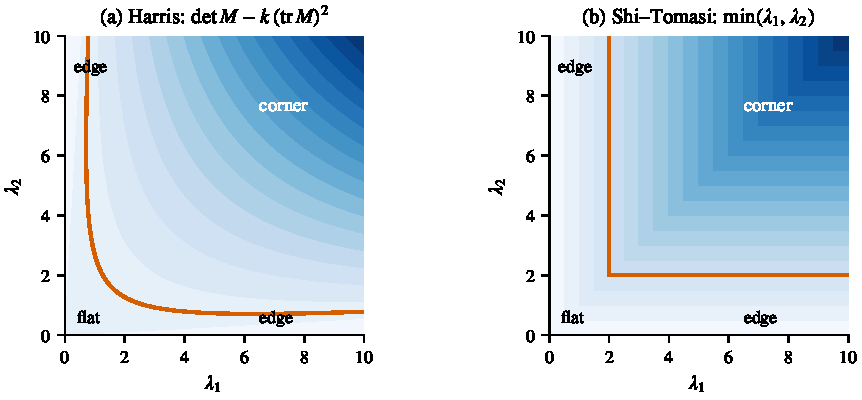
\includegraphics[width=\textwidth]{fig_structure_tensor.pdf}
  \caption{Corner scores over the plane of structure-tensor eigenvalues, with a threshold contour (orange). Both scores accept only windows with two large
  eigenvalues. Shi--Tomasi's $\min(\lambda_1, \lambda_2)$ is exactly the quantity that makes the Lucas--Kanade system well conditioned.}
  \label{fig:structure-tensor}
\end{figure}

\begin{figure}[t]
  \centering
  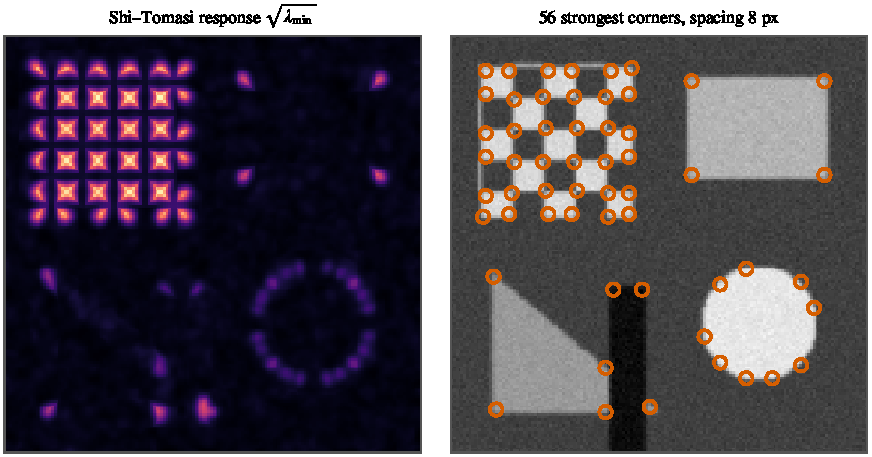
\includegraphics[width=\textwidth]{fig_harris.pdf}
  \caption{Shi--Tomasi corner response on a synthetic image (left), and the strongest corners after non-maximum suppression with a minimum spacing of 8~px (right).
  Edges and flat regions get low scores; corners and blob-like texture get high ones.}
  \label{fig:harris}
\end{figure}

Other detectors trade quality for speed. FAST classifies a pixel as a corner if a long enough arc of the 16 pixels on a circle around it is uniformly brighter or
darker than the center, using only comparisons; it is very fast but noisier. Detectors used for matching across large viewpoint changes add \emph{scale}
selection (detecting at several pyramid levels) and an \emph{orientation} for each feature, as ORB does. A frame-to-frame tracker needs neither.

% ==============================================================================
\section{Lucas--Kanade optical flow}

\subsection{Brightness constancy and the aperture problem}

Assume that a scene point keeps its brightness between consecutive frames, $I_{k+1}(x + d) = I_k(x)$, where $d$ is the image motion of the point. Linearizing in $d$,
\begin{equation}
  I_{k+1}(x) + \nabla I\T d \approx I_k(x)
  \quad\Longleftrightarrow\quad
  I_u\,d_u + I_v\,d_v + I_t = 0, \qquad I_t = I_{k+1}(x) - I_k(x).
  \label{eq:ofc}
\end{equation}
This \emph{optical-flow constraint} is one equation in two unknowns. It determines only the component of $d$ along the gradient: motion along an edge is invisible.
This is the \term{aperture problem}, the same phenomenon seen through a small hole when a long line slides past: only its perpendicular motion is visible.

\subsection{The Lucas--Kanade solution}

\index{Lucas--Kanade tracker}
Lucas and Kanade~\cite{lucas1981iterative} assume the displacement is the same for all pixels of a small window, which provides many equations for the two
unknowns, and solve \eqref{eq:ofc} for all of them in the least-squares sense:
\begin{equation}
  \min_d \sum_{x\in W}w(x)\big(\nabla I(x)\T d + I_t(x)\big)^2
  \quad\Longrightarrow\quad
  M\,d = -\sum_{x\in W}w(x)\,I_t(x)\,\nabla I(x),
  \label{eq:lk}
\end{equation}
with the structure tensor $M$ of \eqref{eq:structure-tensor} as the normal matrix (\cref{sec:least-squares}). The system is solvable and well conditioned exactly when both
eigenvalues of $M$ are large compared with the image noise: Shi and Tomasi's insight was to select features by the very criterion that makes them trackable. With
image noise of variance $\sigma_I^2$ per pixel, the covariance of the estimated displacement is approximately $\sigma_I^2M\inv$ (\cref{prop:wls-cov}), so $1/\sqrt{\lambda_2}$ measures
how precisely the worst direction is tracked.

\subsection{Iterative refinement}

\Cref{eq:lk} rests on a linearization that holds only for small $d$. The full problem, minimizing $\sum_xw(x)(I_{k+1}(x + d) - I_k(x))^2$ over $d$, is a nonlinear least-squares
problem, and Lucas--Kanade is its Gauss--Newton solution (\cref{ch:nlls}):

\begin{algorithm}[h]
\caption{Iterative Lucas--Kanade for one feature}
\label{alg:lk}
\begin{algorithmic}[1]
\Require images $I_k$, $I_{k+1}$; feature position $x_0$; initial guess $d$ (zero, or a prediction)
\State compute the template $T(x) = I_k(x)$ and its gradients over the window around $x_0$; compute $M$ and factor it
\Repeat
  \State sample $I_{k+1}(x + d)$ over the window with bilinear interpolation (\cref{sec:interpolation})
  \State $e(x) \gets I_{k+1}(x + d) - T(x)$ \Comment{residual image}
  \State solve $M\,\Delta d = -\sum_xw(x)\,e(x)\,\nabla T(x)$
  \State $d \gets d + \Delta d$
\Until{$\|\Delta d\| < 0.01$~px or the iteration limit is reached}
\end{algorithmic}
\end{algorithm}

Using the gradients of the \emph{template} $T = I_k$ rather than of the warped image lets $M$ be computed and factored once per feature (the \emph{inverse
compositional} idea, analyzed by Baker and Matthews~\cite{baker2004lk}). Sub-pixel accuracy comes from the bilinear interpolation. A few iterations usually
suffice when the initial guess is within the window radius.

\subsection{Pyramids}

The linearization is valid only for displacements smaller than the scale over which the image gradient is roughly constant, about the window radius. Fast motion
violates this: at 1~rad/s and 20~Hz, the image moves by about 23~px between frames. The remedy is a Gaussian pyramid (\cref{sec:pyramids}). Tracking starts at the
coarsest level, where a 24-pixel motion becomes a 3-pixel motion; the result, doubled, initializes the next finer level, and so on down to full resolution
(\cref{fig:pyramid})~\cite{bouguet2001pyramidal}. With $L$ levels above the base, the trackable displacement grows by about $2^L$.

\begin{figure}[t]
\centering
\begin{tikzpicture}[scale=0.9]
  \foreach \l/\s/\y in {0/3.2/0, 1/1.6/2.0, 2/0.8/3.2, 3/0.4/3.95} {
    \draw[fill=primarylight, draw=primary] (-\s, \y) -- (\s, \y) -- ({\s*0.75}, {\y + 0.35}) -- ({-\s*0.75}, {\y + 0.35}) -- cycle;
    \node[font=\footnotesize, right] at ({\s + 0.2}, {\y + 0.15}) {level \l: $\frac{1}{2^{\l}}$ resolution};
  }
  \draw[->, plotorange, thick] (-0.3,4.2) -- (-0.15,3.55) -- (0.2,2.4) -- (0.9,0.25);
  \node[plotorange, font=\footnotesize, align=right, left] at (-2.0,3.2) {coarse estimate,\\refined at each level};
\end{tikzpicture}
\caption{Pyramidal tracking. A displacement that is too large to linearize at full resolution is small at the top level; each level doubles the estimate and refines
it.}
\label{fig:pyramid}
\end{figure}

\begin{figure}[t]
  \centering
  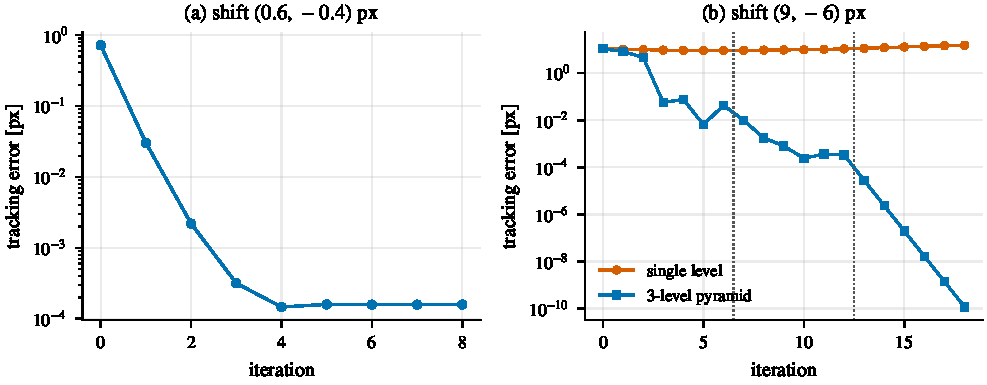
\includegraphics[width=\textwidth]{fig_lk.pdf}
  \caption{Lucas--Kanade on a synthetic textured image. (a) For a small shift of $(0.6, -0.4)$~px, the tracking error falls by orders of magnitude in a few
  Gauss--Newton iterations. (b) For a shift of $(9, -6)$~px, single-level tracking stalls in a wrong local minimum, while a three-level pyramid converges.}
  \label{fig:lk}
\end{figure}

\subsection{When tracking fails}

Lucas--Kanade fails when its assumptions fail: on edges and flat regions (an ill-conditioned $M$, the aperture problem); under occlusion, when the point disappears
behind another object; under strong brightness changes (\cref{ch:imageproc}); under motion blur, which smears the texture the tracker relies on; and when the
window straddles a depth discontinuity, where the two halves move differently. Most failures go undetected by the tracker itself, which returns a confident but wrong
position. Hence the checks of the next section.

% ==============================================================================
\section{Making tracking robust}

Optical flow optimizes photometric similarity, not physical correctness. It will track the shadow of a moving object, a specular highlight, or a T-junction formed by
two objects at different depths. Several layers of checks remove such tracks.
\begin{enumerate}
  \item \textbf{Forward-backward consistency.} Track each point from frame $k$ to $k+1$, then back to $k$. A correct track returns to its starting point; reject it if
        the round-trip error exceeds a fraction of a pixel.
  \item \textbf{IMU-aided prediction.} The gyroscope predicts the rotation between frames, $R_{c_2c_1} = R_{bc}\T R_{b_1b_2}\T R_{bc}$, where $R_{b_1b_2}$ is the integrated gyro rotation.
        For distant points, or a purely rotating camera, image points move by the infinite homography (\cref{ch:camera}): in pixels,
        $\tilde u_2 \propto KR_{c_2c_1}K\inv\tilde u_1$ (after undistortion). Starting LK from this prediction gives it a much better initial guess, and allows smaller windows and
        fewer pyramid levels.
  \item \textbf{Geometric verification.} Reject tracks that violate the epipolar constraint, with essential-matrix or two-point RANSAC, or the rotation-only constraint under
        low parallax (\cref{ch:multiview}).
  \item \textbf{Statistical gating in the filter.} Tracks that pass all of the above are still gated by the $\chi^2$ test of the MSCKF update (\cref{ch:msckfupdate}).
\end{enumerate}

\subsection{Feature distribution}

Asking a detector for the 200 strongest corners typically returns clusters on the most textured object in view. Clustered features constrain the motion poorly:
features in a small patch of the image make rotation and translation hard to separate. The standard remedy is \emph{grid bucketing}: divide the image into cells
(for example $8\times6$) and cap the number of features per cell, plus a minimum distance between features. New features are detected only in cells that have fallen
below their quota, using a mask around existing tracks. A uniform distribution of bearings makes the stacked measurement Jacobian better conditioned, which is
exactly what the estimator needs.

% ==============================================================================
\section{The feature life cycle}

\begin{figure}[h]
\centering
\begin{tikzpicture}[node distance=13mm and 34mm, every node/.style={font=\small}]
  \node[block] (new) {NEW};
  \node[block, right=of new] (trk) {TRACKED};
  \node[block, right=of trk] (lost) {LOST};
  \node[block, below=of trk, fill=white] (used) {consumed by update\\or discarded};
  \draw[->, thick] (new) -- node[above, font=\footnotesize]{tracked} (trk);
  \draw[->, thick] (trk) edge[loop above] node[above, font=\footnotesize]{tracked again} (trk);
  \draw[->, thick] (trk) -- node[above, font=\footnotesize]{track fails} (lost);
  \draw[->, thick] (lost) |- (used);
  \draw[->, thick] (trk) -- node[right, font=\footnotesize, align=left]{oldest observation's\\clone leaving the window} (used);
  \draw[->, thick] (new) |- node[left, font=\footnotesize, pos=0.25]{rejected} (used);
\end{tikzpicture}
\caption{Feature life cycle. A track is handed to the MSCKF update when it is lost, or when its oldest observation is about to leave the sliding window
(AGENTS.md F5). Its observations are used once and then discarded.}
\label{fig:lifecycle}
\end{figure}

Each feature has a persistent ID and a history of observations: (clone index or image timestamp, normalized coordinates). Since the estimator can only use
observations made at times that still have a clone in the window, the history never needs to exceed \code{kMaxClones} entries. That makes it possible to store all
tracks in a fixed-capacity pool with fixed-capacity histories, so the steady state of the front end performs no allocation for its bookkeeping (Milestone 9).

\begin{pitfall}[using a measurement twice]
Once a track's observations have been used in an MSCKF update, they must never be used again, not even partially. Re-using them double counts the same information
and makes the filter overconfident. If a track continues after being used (because its oldest clone was marginalized), its subsequent observations start a fresh
track.
\end{pitfall}

% ==============================================================================
\section{Engineering the front end}

The front end is the one component allowed to allocate (AGENTS.md E4), because OpenCV allocates internally, but it must reuse its buffers. In practice: keep the
previous pyramid and swap it with the new one instead of rebuilding storage; preallocate point vectors with \code{reserve}; keep the \code{cv::Mat} objects as members
so that their memory is reused when sizes do not change; and \emph{measure} the remaining allocations with the allocation guard rather than claiming they are zero.
Feature tracking is typically the most expensive part of the pipeline in time, too, so bucketing parameters, window size and pyramid depth are the main
performance knobs.

Descriptor-based front ends (ORB, BRIEF) describe each feature by a binary string of intensity comparisons in its neighborhood and match features across frames by
the Hamming distance between descriptors, rejecting ambiguous matches whose best and second-best distances are similar (the \emph{ratio test}). They handle large
viewpoint changes and re-detection after occlusion, which matters for loop closure, but for frame-to-frame VIO at 20~Hz KLT tracking is cheaper and more accurate.
Direct methods skip features altogether and use photometric error in the estimator itself.

\begin{projectlink}[Milestones 8 and 9]
M8 builds detection, bucketing, pyramidal LK with forward-backward checks, persistent IDs and point undistortion, and tests them on synthetic images with known
sub-pixel motion. M9 adds the life-cycle manager with a fixed-capacity pool and essential-matrix RANSAC in normalized coordinates, including the documented
pure-rotation behavior.
\end{projectlink}

\begin{takeaways}
\begin{itemize}
  \item The structure tensor $M$, from a first-order expansion of the patch auto-correlation, measures how well a window's position is defined; corners have two
        large eigenvalues.
  \item Lucas--Kanade is Gauss--Newton on the patch alignment error; its normal matrix is $M$, so good corners are exactly the trackable windows.
  \item The aperture problem: a single pixel constrains only the flow along the gradient.
  \item Pyramids extend the trackable displacement; gyro prediction makes tracking cheaper and more robust.
  \item Bucketing spreads features for good geometry; forward-backward checks and RANSAC remove bad tracks.
  \item Tracks are consumed exactly once and their histories are bounded by the window size.
\end{itemize}
\end{takeaways}

\begin{exercises}
  \item Compute the structure tensor of an ideal step edge and of an ideal corner, and verify the eigenvalue picture.
  \item Derive the closed-form smallest eigenvalue of a symmetric $2\times2$ matrix used by the Shi--Tomasi detector.
  \item Implement \cref{alg:lk} for a synthetic textured image translated by $(0.3, -0.7)$ pixels and reproduce \cref{fig:lk}(a). What happens with a translation of
        8~pixels, and how many pyramid levels fix it?
  \item Show that the forward-backward error of a correct track is due only to noise and interpolation, and estimate a sensible threshold.
  \item Compute the pixel displacement predicted by the gyroscope for a feature at the image center when the camera rotates by $0.05$~rad about its $y$-axis between frames.
  \item Implement grid bucketing and plot the feature distribution with and without it on a EuRoC image.
  \item Design the data structure for the feature pool with fixed capacity and per-feature histories bounded by \code{kMaxClones}. What happens when the pool is full?
\end{exercises}
% Solutions to the exercises of Chapter 22.
\begin{solutions}
  \item For a straight edge with unit normal $n$, every gradient in the window is parallel to $n$, $\nabla I = g(x)\,n$, so
        \[
          M = \Big(\sum_xw(x)g(x)^2\Big)\,nn\T,
        \]
        of rank one: eigenvalues $\lambda_1 = \sum_xwg^2$ and $\lambda_2 = 0$, with the null eigenvector along the edge. For a vertical step of height $h$ in a $15\times15$ uniform window with
        central differences, each row has two pixels with $I_u = h/2$, so $M = \diag(7.5h^2, 0)$. For an ideal corner (a bright quadrant) with the window centered on
        its tip, each edge covers half the window: $M = h^2\big[\begin{smallmatrix} 4 & 0.25 \\ 0.25 & 4\end{smallmatrix}\big]$ with eigenvalues $3.75h^2$ and $4.25h^2$, both large; the small
        off-diagonal entry comes from the tip pixel, where both gradients are non-zero. More generally, two edges of equal strength $c$ with normals at an
        angle $\alpha$ give $M = c(n_1n_1\T + n_2n_2\T)$ with eigenvalues $c(1 \pm \cos\alpha)$: a right-angle corner is ideal, while a sharp wedge (normals $20^\circ$ apart,
        $\lambda_2 = 0.06c$) is poorly localized along its bisector.

  \item The characteristic polynomial of $M = \big[\begin{smallmatrix} a & b \\ b & c\end{smallmatrix}\big]$ is $\lambda^2 - (\tr M)\lambda + \det M$, so $\lambda = \tfrac12\big(\tr M \pm \sqrt{(\tr M)^2 - 4\det M}\big)$.
        The discriminant is
        \[
          (a + c)^2 - 4(ac - b^2) = (a - c)^2 + 4b^2 \ge 0,
        \]
        so both roots are real (as they must be for a symmetric matrix) and
        $\lambda_{\min} = \tfrac12\big(a + c - \sqrt{(a - c)^2 + 4b^2}\big)$. Use the second form in code: $(\tr M)^2 - 4\det M$ subtracts two nearly equal numbers when the eigenvalues
        are close, and rounding can make it slightly negative, which turns the square root into a NaN.

  \item On a texture smoothed with $\sigma = 2$~px (as in \cref{fig:lk}) and a $21\times21$ window, the shift $(0.3, -0.7)$ gives errors of $0.76$, $0.022$ and $0.010$~px after
        zero, one and two iterations, and then stalls at $0.010$~px. The floor is the bias of bilinear interpolation, since the shifted image was generated with
        cubic interpolation. With cubic sampling the error keeps falling, as in the figure. For a shift of 8~px and a $15\times15$ window, single-level tracking is correct to
        $0.1$~px from only 30--45\% of window positions: elsewhere it converges to a wrong local minimum. The texture decorrelates over a few pixels (the
        autocorrelation is $0.58$ at 3~px and $0.26$ at 5~px), so the linearization holds only for displacements of about 2--3~px. With one pyramid level above the
        base, the displacement there is 4~px and 93--98\% succeed; with two levels it is 2~px and all succeed. The rule: choose $L$ so that the largest expected
        displacement divided by $2^L$ is within the texture's correlation length.

  \item Let the true motion be $d$. The forward track returns $\hat d_f = d + e_f$ and the backward track, started at $x + \hat d_f$, returns $\hat d_b = -d + e_b$, where $e_f$ and $e_b$
        are the estimation errors of the two tracks. The round-trip error is $\hat d_f + \hat d_b = e_f + e_b$: the true motion cancels exactly, whatever its size. For a track
        that converged to the right minimum, only the causes of estimation error remain: image noise, interpolation and the convergence tolerance. Without them,
        both tracks would be exact. Moreover, $e_b \approx -e_f$: the backward window is centered on $x + \hat d_f$, so both directions compare the same pixel pairs of
        the same two images. In a simulation with noise of 1\% of the intensity range ($15\times15$ window), the forward tracking error has a median of $0.03$~px,
        but the round-trip error only $0.001$~px (99th percentile $0.005$~px), and $10^{-4}$~px without noise. The check tests self-consistency, not accuracy. Failures are a different matter: when half of the window is occluded in the
        second image, the median round-trip error is $1.7$~px, and 97\% exceed $0.1$~px. Real images add deformation, blur and brightness change, which
        raise the errors of correct tracks, so a threshold of a few tenths of a pixel keeps a wide margin while catching most failures. Better still, set it
        from a histogram of round-trip errors on a real sequence: correct tracks form a sharp peak near zero and failures a long tail.

  \item A rotation by $\theta = 0.05$~rad about the camera's $y$-axis turns the optical axis toward $+x_c$, so $R_{c_2c_1} = R_y(\theta)\T$. The feature at the principal point has
        bearing $(0, 0, 1)$, which becomes $R_y(\theta)\T(0, 0, 1)\T = (-\sin\theta, 0, \cos\theta)$, so
        \[
          u_2 = c_u - f_u\tan\theta = c_u - 22.95, \qquad v_2 = c_v :
        \]
        the feature moves 23~px to the left, the same as $KR_{c_2c_1}K\inv\tilde u_1$ gives. The prediction does not depend on depth; the neglected translation, 1~m/s
        over 50~ms at 5~m depth for example, adds only $f_u\cdot0.05/5 \approx 4.6$~px, which LK recovers easily from the predicted start.

  \item Divide the image into cells (for example $8\times6$ cells of $94\times80$~px for EuRoC). Compute the corner response once, with non-maximum suppression and
        one global threshold. Then take candidates strongest first, skipping any in a cell that has reached its quota or within the minimum distance of an
        existing track or an already chosen corner. Count the existing features per cell before detecting, so that only depleted cells receive new ones. To
        evaluate, report two numbers: the fraction of occupied cells, and the spread of the feature bearings (the standard deviations along the principal
        axes of their covariance, after undistortion). The script \code{scripts/solutions/ch22\_bucketing.py} does this for 150 corners, 10~px apart, with and
        without a quota of 4 per cell. It uses the first frame of \code{data/MH\_01\_easy} when the dataset is present. On a synthetic $752\times480$ image with one strongly
        textured region and weak texture elsewhere (one fifth of the contrast):
        \begin{center}\small
        \begin{tabular}{@{}l c c c@{}}
        \toprule
        selection & occupied cells & most corners in a cell & bearing spread (rad) \\
        \midrule
        strongest 150 & 46\% & 18 & 0.26 / 0.21 \\
        bucketed, at most 4 per cell & 96\% & 4 & 0.55 / 0.32 \\
        \bottomrule
        \end{tabular}
        \end{center}
        Without bucketing, every corner lies on the textured region and half of the view is empty. With bucketing, the corners cover nearly every cell, and
        the bearings spread twice as wide along the long axis of the image, which is what conditions the stacked Jacobian. Bucketing redistributes corners
        but cannot create texture: with a global threshold, cells whose texture is below it stay empty. That is the right outcome, since a corner too weak
        to pass the threshold is also too weak to track.

  \item A pool of fixed capacity $F_{\max}$ (at least the per-cell quota times the number of cells, plus room for tracks that are lost but not yet processed):
        \begin{itemize}
          \item an array of $F_{\max}$ track slots, each with a 64-bit ID, a status (free, new, tracked, lost), a count, and a fixed array of \code{kMaxClones}
                observations $\{$clone ID or timestamp, normalized $(x, y)\}$;
          \item a stack of free slot indices, so allocation and release are $O(1)$, and parallel fixed-capacity arrays of the current pixel positions and slot
                indices, which are what the LK call consumes;
          \item IDs that increase monotonically and are never reused, so stale references are detectable.
        \end{itemize}
        The history cannot overflow: when the oldest clone of a track leaves the window, the track is consumed (AGENTS.md F5), and any continuation starts a new
        history. If the pool is full, the simplest correct policy is to detect no new features until slots free up; the alternative is to evict the weakest
        (shortest or lowest-score) tracks. Either way the event is counted and logged, and the capacity is sized so that it does not happen in normal
        operation. Discarding a track loses information but never corrupts the estimate, unlike reusing one.
\end{solutions}


\chapter{Multiple-View Geometry}
\label{ch:multiview}

\begin{objectives}
\begin{itemize}
  \item Derive the epipolar constraint, the essential and fundamental matrices, epipoles and epipolar lines.
  \item Recover relative motion from correspondences: the eight-point algorithm with normalization, the five-point and two-point methods, and the
        decomposition of the essential matrix.
  \item Understand homographies between views, the pure-rotation case, and the degeneracies of relative-pose estimation.
  \item Use RANSAC to reject outliers, size its iteration count, and set thresholds in the right units.
  \item Triangulate points by midpoint, linear and Gauss--Newton methods, and quantify triangulation accuracy.
  \item Understand bundle adjustment, its sparsity and its gauge freedom: the batch problem the MSCKF approximates.
\end{itemize}
\end{objectives}

% ==============================================================================
\section{Epipolar geometry}

\subsection{The epipolar constraint}

Two cameras observe the same 3D point. Let the coordinates of the point in the two camera frames be $X_1$ and $X_2$, related by the rigid motion
\begin{equation}
  X_2 = R\,X_1 + t, \qquad R = R_{c_2c_1},\quad t = p_{c_2c_1},
\end{equation}
and let $\bar x_1 = X_1/Z_1$ and $\bar x_2 = X_2/Z_2$ be the bearings (homogeneous normalized coordinates).

\begin{theorem}[Epipolar constraint]
\label{thm:epipolar}
\index{epipolar constraint}\index{essential matrix}
Every correspondence of a rigid point satisfies
\begin{equation}
  \bar x_2\T\,E\,\bar x_1 = 0, \qquad E = \sx{t}\,R .
  \label{eq:epipolar}
\end{equation}
\end{theorem}
\begin{proof}
Cross both sides of $X_2 = RX_1 + t$ with $t$: $\sx{t}X_2 = \sx{t}RX_1$. The left side is orthogonal to $X_2$, so $X_2\T\sx{t}RX_1 = 0$. Dividing by $Z_1Z_2 > 0$ gives
\eqref{eq:epipolar}.
\end{proof}

Geometrically, the two camera centers and the 3D point span a plane, the \emph{epipolar plane}, and the constraint states that the two viewing rays and the baseline
are coplanar (\cref{fig:epipolar}). The constraint involves no depth: it is a statement about bearings only, which is why it is the natural tool for checking tracks
before any 3D reconstruction exists.

\begin{figure}[t]
\centering
\begin{tikzpicture}[scale=1.0]
  \coordinate (C1) at (0,0); \coordinate (C2) at (5,0.3); \coordinate (P) at (2.7,3.4);
  \fill[primarylight, opacity=0.7] (C1) -- (C2) -- (P) -- cycle;
  \draw[thick] (C1) -- (C2) node[midway, below] {baseline $t$};
  \draw[plotgreen, thick] (C1) -- (P); \draw[plotgreen, thick] (C2) -- (P);
  \fill (C1) circle (1.8pt) node[below left] {$C_1$};
  \fill (C2) circle (1.8pt) node[below right] {$C_2$};
  \fill[conv] (P) circle (2pt) node[above] {$p_f$};
  \draw[primary, thick] (0.3,1.5) -- (1.6,1.2) -- (1.6,0.2) -- (0.3,0.5) -- cycle;
  \draw[primary, thick] (3.5,1.3) -- (4.8,1.7) -- (4.8,0.7) -- (3.5,0.3) -- cycle;
  \fill[plotgreen] ($(C1)!0.3!(P)$) circle (1.5pt) node[left, font=\footnotesize] {$\bar x_1$};
  \fill[plotgreen] ($(C2)!0.3!(P)$) circle (1.5pt) node[right, font=\footnotesize] {$\bar x_2$};
  \draw[conv, dashed] (3.6,0.65) -- (4.75,1.45);
  \node[conv, font=\footnotesize, anchor=west] at (5.0,1.25) {epipolar line $E\bar x_1$};
  \node[font=\footnotesize, primary] at (2.6,1.7) {epipolar plane};
\end{tikzpicture}
\caption{Epipolar geometry. The camera centers, the point and both viewing rays lie in one plane. The image of the point in the second camera must therefore lie on
the line where that plane cuts the second image.}
\label{fig:epipolar}
\end{figure}

\subsection{Epipolar lines and epipoles}

Given $\bar x_1$, the vector $\ell_2 = E\bar x_1$ represents a line in the second image (\cref{sec:homogeneous}), the \term{epipolar line}: the corresponding point must lie on
it. Searching for a match can be restricted to this line. All epipolar lines in the second image pass through the \term{epipole} $e_2$, the image of the first camera
center, which satisfies $e_2\T E = 0$ (it is proportional to $t$); symmetrically $Ee_1 = 0$ with $e_1 \propto R\T t$. When the camera moves forward, the epipole is the
\emph{focus of expansion} from which image points flow outward.

\begin{proposition}[Properties of the essential matrix]
\label{prop:essential}
For $t \ne 0$, $E = \sx{t}R$ has rank two and two equal non-zero singular values, $(\|t\|, \|t\|, 0)$. It has five degrees of freedom: three for the rotation and two for the
direction of $t$. Its overall scale, like the scale of $t$, is unobservable.
\end{proposition}
\begin{proof}
$EE\T = \sx{t}RR\T\sx{t}\T = -\sx{t}^2 = \|t\|^2I - tt\T$ by \eqref{eq:skew-sq}, whose eigenvalues are $\|t\|^2$ (twice, on the plane orthogonal to $t$) and $0$ (along $t$). The
singular values of $E$ are their square roots.
\end{proof}

In pixel coordinates, with $\tilde u_i = K\bar x_i$, the constraint reads $\tilde u_2\T F\tilde u_1 = 0$ with the \term{fundamental matrix} $F = K\mT EK\inv$ (seven degrees of freedom,
rank two). The project works with undistorted normalized coordinates throughout, so it uses $E$ directly (Milestone 9).

% ==============================================================================
\section{Estimating relative motion}

\subsection{The eight-point algorithm}

\Cref{eq:epipolar} is linear in the nine entries of $E$. Writing $\bar x_1 = (x_1, y_1, 1)$ and $\bar x_2 = (x_2, y_2, 1)$, each correspondence gives one equation
\begin{equation}
  a\T e = 0, \qquad a = (x_2x_1,\ x_2y_1,\ x_2,\ y_2x_1,\ y_2y_1,\ y_2,\ x_1,\ y_1,\ 1), \qquad e = \vect_{\text{rows}}(E).
\end{equation}
With eight or more correspondences, stack them into $Ae = 0$ and take the unit vector minimizing $\|Ae\|$: the right singular vector of $A$ with the smallest
singular value (\cref{prop:homogeneous-ls}). Noise makes the result an invalid essential matrix, which is projected onto the nearest valid one by replacing its
singular values with $(1, 1, 0)$ (\cref{thm:svd} and Eckart--Young). When the algorithm is applied to pixel coordinates (to estimate $F$), the coordinates must first
be \emph{normalized} (translated to zero mean and scaled to unit average distance from the origin), or the matrix $A$, whose entries range from 1 to $10^5$, is so
badly conditioned that the result is unusable; this is Hartley's normalization.

\subsection{Decomposing the essential matrix}

\begin{proposition}[Motion from the essential matrix]
\label{prop:e-decomposition}
Let $E = U\diag(1, 1, 0)V\T$ with $U, V$ rotations (flip their signs if needed), and $W = \begin{bmatrix}0 & -1 & 0\\ 1 & 0 & 0\\ 0 & 0 & 1\end{bmatrix}$. The rotation and translation
direction are one of the four combinations
\begin{equation}
  R \in \{UWV\T,\ UW\T V\T\}, \qquad t \in \{+u_3,\ -u_3\},
\end{equation}
where $u_3$ is the third column of $U$. Exactly one of the four places triangulated points in front of both cameras.
\end{proposition}

The proof checks that $\sx{u_3}UWV\T$ and $\sx{u_3}UW\T V\T$ both equal $E$ up to sign, and that no other factorizations exist. The four solutions correspond to the second
camera being on either side of the first, facing either forward or backward; the \emph{cheirality} test (positive depth of a triangulated point in both views)
selects the physical one.

\subsection{The five-point and two-point methods}

Five correspondences are the minimum, since $E$ has five degrees of freedom. Nistér's algorithm~\cite{nister2004five} combines the linear constraints of five
correspondences with the cubic constraints that characterize essential matrices ($\det E = 0$ and $2EE\T E - \tr(EE\T)E = 0$) and solves the resulting polynomial system,
returning up to ten candidates. Fewer points per hypothesis means fewer RANSAC iterations, which is why \code{cv::findEssentialMat} uses it.

In VIO the gyroscope supplies the relative rotation $R$ between consecutive frames with high accuracy. With $R$ known, \eqref{eq:epipolar} becomes linear in $t$:
\begin{equation}
  \bar x_2\T\sx{t}R\bar x_1 = t\T\big(R\bar x_1\times\bar x_2\big) = 0 .
\end{equation}
Each correspondence says that $t$ is orthogonal to the vector $c_i = R\bar x_1^{(i)}\times\bar x_2^{(i)}$, so two correspondences determine the direction of $t$ as $c_1\times c_2$. A two-point
hypothesis needs far fewer RANSAC iterations than a five-point one, and it is the outlier-rejection strategy of MSCKF-VIO~\cite{sun2018msckfvio}.

\subsection{Measuring the residual}

The algebraic residual $\bar x_2\T E\bar x_1$ has no geometric meaning. The geometric error of a correspondence is the smallest displacement of $\bar x_1$ and $\bar x_2$ that
makes the constraint hold exactly. Linearizing the constraint in that displacement gives the \emph{Sampson distance}
\begin{equation}
  d_S = \frac{(\bar x_2\T E\bar x_1)^2}{(E\bar x_1)_1^2 + (E\bar x_1)_2^2 + (E\T\bar x_2)_1^2 + (E\T\bar x_2)_2^2},
\end{equation}
the squared residual divided by the squared norm of its gradient with respect to the four image coordinates: the first-order squared distance to the constraint
surface. It is in the units of the coordinates used. With normalized coordinates, a pixel threshold $\tau_{px}$ must be converted to $\tau_{px}/f$ (Milestone 9).

\begin{pitfall}[thresholds in the wrong units]
Calling \code{cv::findEssentialMat} on normalized coordinates with an identity camera matrix and a threshold of ``1.0'' accepts residuals of 1 normalized unit, about
450 pixels: every track becomes an inlier. The threshold must be $\tau_{px}/f$, e.g.\ $1/458 \approx 2.2\times10^{-3}$.
\end{pitfall}

% ==============================================================================
\section{Homographies between views}
\label{sec:homographies}

\paragraph{Planar scenes.} If all points lie on a plane $n\T X_1 = d$ (unit normal $n$ and distance $d$ in the first camera's frame), then $1 = n\T X_1/d$ and
$X_2 = RX_1 + t\,n\T X_1/d$, so
\begin{equation}
  X_2 = \Big(R + \frac{t\,n\T}{d}\Big)X_1, \qquad \bar x_2 \propto H\bar x_1, \quad H = R + \frac{tn\T}{d} .
\end{equation}
\paragraph{Pure rotation.} If $t = 0$, $X_2 = RX_1$ for every point, at any depth: $\bar x_2 \propto R\bar x_1$, the \emph{infinite homography}. In pixels it is $KRK\inv$.

A homography has eight degrees of freedom and is estimated from four or more correspondences by a direct linear transform: each correspondence gives two linear
equations in the nine entries of $H$ (from $\tilde x_2\times H\tilde x_1 = 0$), solved by \cref{prop:homogeneous-ls}.

% ==============================================================================
\section{RANSAC}

Random Sample Consensus~\cite{fischler1981ransac} estimates a model from data containing outliers by hypothesis and verification.

\begin{algorithm}[h]
\caption{RANSAC}
\begin{algorithmic}[1]
\Require data, minimal sample size $s$, threshold $\tau$, confidence $p$
\State best $\gets \emptyset$; $N \gets \infty$; $k \gets 0$
\While{$k < N$}
  \State draw $s$ data points at random; fit candidate models
  \State count inliers with residual $< \tau$; keep the model with the most inliers
  \State update $N$ from the current inlier ratio $w$ with \eqref{eq:ransac-n}; $k \gets k + 1$
\EndWhile
\State refit the model on all inliers of the best hypothesis (least squares)
\end{algorithmic}
\end{algorithm}

If a fraction $w$ of the data are inliers, a random minimal sample is outlier-free with probability $w^s$, and $N$ independent samples all contain an outlier with probability
$(1 - w^s)^N$. Requiring this to be at most $1 - p$ gives the number of iterations
\begin{equation}
  N = \frac{\log(1 - p)}{\log(1 - w^s)} .
  \label{eq:ransac-n}
\end{equation}
\begin{center}\small
\begin{tabular}{@{}l c c c@{}}
\toprule
$p = 0.99$ & $w = 0.9$ & $w = 0.7$ & $w = 0.5$ \\
\midrule
8-point ($s = 8$) & 9 & 78 & 1177 \\
5-point ($s = 5$) & 6 & 26 & 146 \\
2-point ($s = 2$) & 3 & 7 & 17 \\
\bottomrule
\end{tabular}
\end{center}
The exponential dependence on $s$ is why minimal solvers matter, and why using the gyroscope to remove three unknowns pays off. Since $w$ is unknown in advance, the
algorithm starts pessimistic and updates $N$ from the best inlier ratio found so far (adaptive termination). Variants score hypotheses by the sum of truncated
residuals (MSAC) rather than the inlier count, or refine the best hypothesis locally (LO-RANSAC).

\begin{figure}[t]
  \centering
  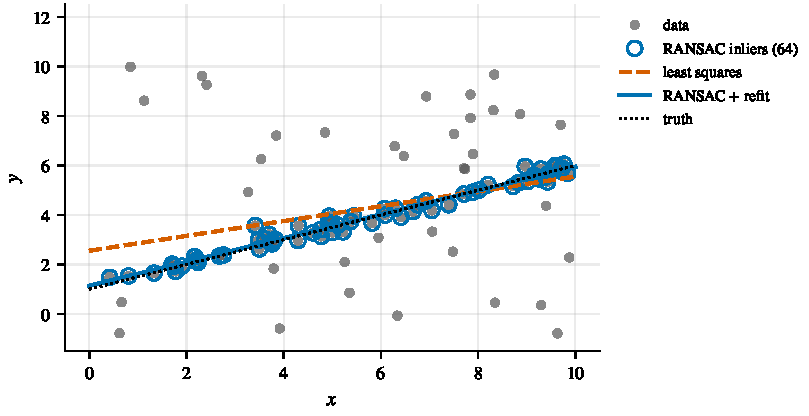
\includegraphics[width=0.86\textwidth]{fig_ransac.pdf}
  \caption{Fitting a line to data with 40\% gross outliers. Least squares is dragged away by the outliers; RANSAC finds the line supported by the most inliers
  (circled) and refits it to them.}
  \label{fig:ransac}
\end{figure}

% ==============================================================================
\section{Degeneracies}

\subsection{Pure rotation}

If the camera only rotates, $t = 0$ and $E = \sx{0}R = 0$: the epipolar constraint is satisfied by every pair of points, inlier or not. Under small translation the problem is
not degenerate but badly conditioned: $t$ is poorly determined, inlier sets fluctuate, and RANSAC may reject good tracks or accept bad ones. Hovering drones rotate in
place often, so this case must be handled (Milestone 9).

Under pure rotation the correspondences satisfy the stronger constraint $\bar x_2 \propto R\bar x_1$ (\cref{sec:homographies}), which does not involve $t$ at all. A robust front end
measures the parallax remaining after rotation compensation, for example the median of $\|\pi(R\bar x_1) - \pi(\bar x_2)\|$ over the tracks:
\begin{itemize}
  \item if it is large, run essential-matrix (or two-point) RANSAC;
  \item if it is tiny, skip epipolar RANSAC and reject only tracks that violate the rotation-only prediction $\bar x_2 \propto R\bar x_1$, with $R$ from the gyroscope.
\end{itemize}
Either way the system keeps tracking: low parallax means the features carry little information about translation, not that they are wrong. The MSCKF update
handles them gracefully, because their nullspace-projected residuals simply contribute little.

\subsection{Other degeneracies}

The eight-point algorithm is degenerate when all points lie on a plane, a common situation (floors, walls), because a homography then explains the data equally well;
the five-point algorithm is not. Very distant points behave like points at infinity and carry only rotational information. Moving objects form a second, consistent
rigid motion that RANSAC can mistake for the dominant one if they fill the image.

% ==============================================================================
\section{Triangulation}
\label{sec:triangulation}

Given observations $z_i$ of a point in cameras with known poses $(R_{wc_i}, p_{wc_i})$, triangulation estimates its world position $p_f$.

\subsection{The midpoint method}

Each observation defines a ray $p_{wc_i} + \lambda_ir_i$ with direction $r_i = R_{wc_i}\bar x_i$. With noise the rays do not intersect. The midpoint method finds the point
closest to all rays in the least-squares sense: the distance of $p$ from ray $i$ is $\|(I - \hat r_i\hat r_i\T)(p - p_{wc_i})\|$ with $\hat r_i$ the unit direction, so
\begin{equation}
  \Big(\sum_i(I - \hat r_i\hat r_i\T)\Big)\,p = \sum_i(I - \hat r_i\hat r_i\T)\,p_{wc_i} .
\end{equation}
It is simple and geometric, but it minimizes 3D distances rather than image errors, which weights distant views wrongly.

\subsection{Linear triangulation}

In camera $i$ the point has coordinates $X_i = R_{wc_i}\T(p_f - p_{wc_i})$, which must be parallel to the bearing $\bar x_i = (z_i, 1)$: $\sx{\bar x_i}X_i = 0$. Substituting,
\begin{equation}
  \sx{\bar x_i}R_{wc_i}\T\, p_f = \sx{\bar x_i}R_{wc_i}\T\, p_{wc_i}, \qquad i = 1,\dots,M .
  \label{eq:dlt}
\end{equation}
Each view contributes three equations of rank two. Stacking all views gives an overdetermined linear system $A p_f = b$ that is solved in the least-squares sense with
QR or SVD. With two views and noise-free data the solution is exact. This is the linear initialization of AGENTS.md F5. It minimizes an algebraic error, not the
reprojection error, so it is refined next.

\subsection{Nonlinear refinement with inverse depth}

The maximum-likelihood estimate minimizes the reprojection error (\cref{ch:nlls})
\begin{equation}
  \min_{p_f}\ \sum_{i=1}^M \big\| z_i - \pi(X_i(p_f)) \big\|^2 .
\end{equation}
The MSCKF~\cite{mourikis2007msckf} parameterizes the point in an \emph{anchor} camera $A$ (for example the first observation) by inverse depth~\cite{civera2008inverse}:
\begin{equation}
  X_A = \frac1\rho\begin{bmatrix} \alpha \\ \beta \\ 1 \end{bmatrix}, \qquad
  X_i = R_{iA}X_A + p_{iA}
  \quad\Longrightarrow\quad
  h_i := \rho X_i = R_{iA}\begin{bmatrix}\alpha\\ \beta\\ 1\end{bmatrix} + \rho\,p_{iA}, \quad z_i = \pi(h_i),
\end{equation}
where $(R_{iA}, p_{iA})$ is the transformation from the anchor camera to camera $i$, computed from the clone poses, and $\pi(h_i) = \pi(X_i)$ because projection ignores scale.
The parameters $(\alpha, \beta)$ are the normalized coordinates in the anchor view and $\rho = 1/Z_A$ is the inverse depth. This parameterization behaves well for distant points
($\rho\to0$ is a regular point), and the measurement function is nearly linear in $(\alpha, \beta, \rho)$. Its Jacobian follows from the chain rule:
\begin{equation}
  \frac{\partial z_i}{\partial(\alpha, \beta, \rho)} = \frac{\partial\pi}{\partial h}\Big|_{h_i}\,
  \begin{bmatrix} r_1 & r_2 & p_{iA} \end{bmatrix},
\end{equation}
where $r_1, r_2$ are the first two columns of $R_{iA}$ and $\partial\pi/\partial h$ is \cref{prop:proj-jacobian}. Gauss--Newton (\cref{alg:gauss-newton}) iterates
$\delta y = -(J\T J)\inv J\T e$ with the stacked Jacobian $J$ and residual $e$, usually converging in a few iterations from the linear initialization. Levenberg--Marquardt
damping adds robustness.

\subsection{How accurate is triangulation?}

For two views separated by a baseline $b$ perpendicular to the viewing direction, the depth is $Z = b/d$ with $d$ the disparity in normalized coordinates. With
independent noise $\sigma_{uv}$ in each view, $\sigma_d = \sqrt2\sigma_{uv}$, and since $\partial Z/\partial d = -b/d^2 = -Z^2/b$, to first order
\begin{equation}
  \sigma_Z \approx \frac{Z^2}{b}\sqrt2\,\sigma_{uv} .
  \label{eq:depth-sigma}
\end{equation}
Depth error grows quadratically with depth and inversely with baseline. Equivalently, the relative depth error is inversely proportional to the parallax angle $\approx b/Z$.

\begin{figure}[t]
  \centering
  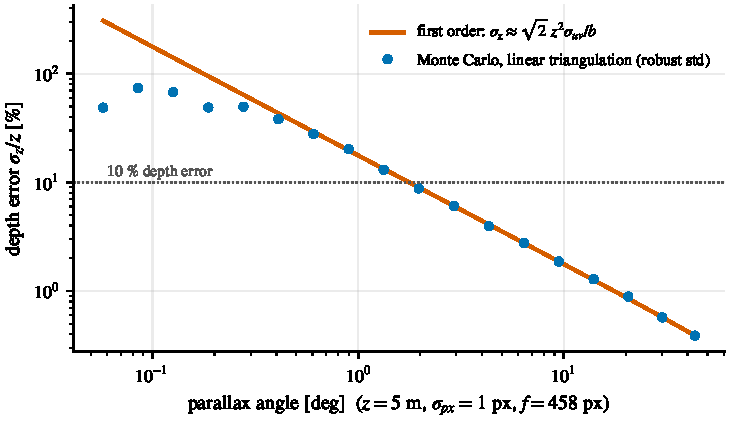
\includegraphics[width=0.86\textwidth]{fig_triangulation.pdf}
  \caption{Relative depth error of two-view triangulation at $Z = 5$~m with 1-pixel noise, versus parallax angle. Down to about $1^\circ$ the first-order formula \eqref{eq:depth-sigma}
  describes the spread accurately. Below that the error distribution becomes heavy-tailed (depths can even become negative), and the estimate is unusable.}
  \label{fig:triangulation}
\end{figure}

\Cref{fig:triangulation} shows that 10\% depth accuracy needs about $2^\circ$ of parallax, a baseline of 17~cm at 5~m. Down to about $1^\circ$ \eqref{eq:depth-sigma} still
describes the bulk of the estimates; below that, outliers take over. At $0.5^\circ$, 4\% of the estimates are off by more than five standard deviations, and at
$0.25^\circ$, 8\% of the depths come out negative. A triangulation module must therefore check its own result before handing it to the filter:
\begin{itemize}
  \item positive depth in every view (cheirality);
  \item sufficient parallax (or baseline relative to depth), or equivalently a well-conditioned Gauss--Newton Hessian;
  \item small reprojection error in every view after refinement;
  \item a plausible depth range.
\end{itemize}
Features that fail are discarded, not fed to the update (AGENTS.md F5, Milestone 10b).

% ==============================================================================
\section{Bundle adjustment}
\label{sec:bundle-adjustment}

\termi{Bundle adjustment}{bundle adjustment} estimates all camera poses and all 3D points at once by minimizing the total reprojection error,
\begin{equation}
  \min_{\{T_i\},\{p_j\}}\ \sum_{(i,j)\text{ observed}}\big\|z_{ij} - \pi\big(T_i\inv p_j\big)\big\|^2_{R\inv},
\end{equation}
with Gauss--Newton or Levenberg--Marquardt on the manifold of poses (\cref{ch:nlls}). It is the gold standard of geometric vision. Two of its properties illuminate
VIO.
\begin{itemize}
  \item \emph{Structure.} Each residual involves one camera and one point, so the normal equations have the block structure of \cref{sec:schur-ba}: eliminating the
        points with the Schur complement leaves a small \emph{reduced camera system} (\cref{fig:ba-sparsity}).
  \item \emph{Gauge freedom.} Moving and rotating everything together, or (for a monocular camera) scaling everything, leaves all reprojection errors unchanged: the
        problem has seven unobservable directions, and $J\T WJ$ is singular along them. Solvers fix the gauge by holding the first camera fixed and the scale constant, or
        by adding a weak prior. With an IMU, scale and two rotation directions (roll and pitch) become observable, and the gauge shrinks to the four directions of
        \cref{ch:observability}.
\end{itemize}
The MSCKF can be understood as a fast, filtered approximation of bundle adjustment over a sliding window: it eliminates each point exactly as the Schur complement
does (\cref{ch:msckfupdate}), takes a single Gauss--Newton step, and summarizes the past by the filter's Gaussian prior instead of relinearizing it.

\paragraph{Pose from known points.} Finally, when the 3D points are known (a map), a single image determines the camera pose: the
\emph{perspective-$n$-point} (PnP) problem, solved minimally from three points and refined by Gauss--Newton. It is the core of relocalization against a map, a
capability that odometry lacks.

\begin{takeaways}
\begin{itemize}
  \item Rigid correspondences satisfy $\bar x_2\T\sx{t}R\bar x_1 = 0$; $E$ has 5 DOF, singular values $(\|t\|, \|t\|, 0)$, and an unobservable scale.
  \item The eight-point algorithm is linear (normalize pixel coordinates first); $E$ decomposes into four motions, one of which passes the cheirality test.
  \item With the rotation from the gyroscope, two correspondences determine the translation direction.
  \item Planes and pure rotations relate views by homographies; under pure rotation $E$ vanishes and the rotation-only constraint takes over.
  \item RANSAC iterations grow as $w^{-s}$: prefer minimal solvers. Thresholds in normalized units are $\tau_{px}/f$.
  \item Triangulate linearly, refine by Gauss--Newton with inverse depth, and reject low-parallax or negative-depth points; depth error grows as $Z^2/b$.
  \item Bundle adjustment is the batch problem; the MSCKF approximates it with exact landmark elimination and a single Gauss--Newton step.
\end{itemize}
\end{takeaways}

\begin{exercises}
  \item Verify \cref{thm:epipolar} numerically for random points and a random relative pose, then show that adding an outlier breaks it.
  \item Prove \cref{prop:essential} and show that $e_2 \propto t$ is the left null vector of $E$.
  \item Implement the eight-point algorithm with and without Hartley normalization on pixel coordinates, and compare the errors.
  \item Implement the decomposition of \cref{prop:e-decomposition} and the cheirality test, and verify on synthetic data that the correct solution is selected.
  \item Implement the two-point method with known rotation inside RANSAC on synthetic data with 30\% outliers. Compare the number of iterations needed with the five-point
        method.
  \item Generate a pure-rotation sequence, observe what \code{cv::findEssentialMat} returns, and implement the parallax test.
  \item Show that \eqref{eq:dlt} has rank two per view and that two views with non-parallel rays give a unique solution.
  \item Derive \eqref{eq:depth-sigma}, reproduce \cref{fig:triangulation}, and repeat with three views over the same baseline.
  \item Count the gauge freedoms of monocular bundle adjustment and of visual-inertial bundle adjustment, and explain the difference.
\end{exercises}
% Solutions to the exercises of Chapter 23.
\begin{solutions}
  \item With 20 random points at 3--8~m and a random relative pose, $|\bar x_2\T E\bar x_1| \le 3\times10^{-17}$: rounding error. Moving one observation in the second image
        by 27~px gives an algebraic residual of $8\times10^{-3}$ and a Sampson distance $\sqrt{d_S}$ of $5.4$~px. Only the component of the error perpendicular to the
        epipolar line is visible (7.7~px of the 27~px here), and the Sampson distance spreads it over both images ($7.7/\sqrt2 = 5.4$). A two-view check cannot
        detect an error \emph{along} the epipolar line at all; a third view, or the filter's own gating, must catch those.

  \item Since $RR\T = I$ and $\sx{t}\T = -\sx{t}$, $EE\T = -\sx{t}^2 = \|t\|^2I - tt\T$ (\eqref{eq:skew-sq}). Every vector orthogonal to $t$ is an eigenvector with eigenvalue
        $\|t\|^2$, and $t$ itself has eigenvalue 0, so the singular values of $E$ are $(\|t\|, \|t\|, 0)$ and its rank is two. Degrees of freedom: $R$ has three and $t$ three,
        but the constraint $\bar x_2\T E\bar x_1 = 0$ is homogeneous, so $E$ and $\lambda E$ (i.e.\ $t$ and $\lambda t$) are indistinguishable: $3 + 2 = 5$. Scaling the scene and
        the baseline together leaves every bearing unchanged, so the scale of $t$ cannot be recovered from images. For the epipoles,
        \[
          t\T E = t\T\sx{t}R = -(\sx{t}t)\T R = -(t\times t)\T R = 0, \qquad E(R\T t) = \sx{t}t = 0 .
        \]
        The left null vector is $t$, the coordinates of the first camera center in the second frame ($X_1 = 0 \Rightarrow X_2 = t$), so $e_2 \propto t$ is its image. Likewise
        $e_1 \propto R\T t$ is the image of the second center ($X_2 = 0 \Rightarrow X_1 = -R\T t$).

  \item With 60 points, 0.5~px noise and 200 random scenes, recovering $(R, t)$ from $E = K\T FK$:
        \begin{center}\small
        \begin{tabular}{@{}l c c c@{}}
        \toprule
        & $\sigma_1/\sigma_8$ of $A$ & rotation error & direction of $t$ \\
        & & median / 90\% & median / 90\% \\
        \midrule
        raw pixels & $1.5\times10^5$ & $0.33^\circ$ / $1.6^\circ$ & $2.5^\circ$ / $11^\circ$ \\
        Hartley-normalized & 66 & $0.16^\circ$ / $0.34^\circ$ & $1.1^\circ$ / $2.4^\circ$ \\
        \bottomrule
        \end{tabular}
        \end{center}
        In pixels, the columns of $A$ range from $1$ to $10^5$, so the smallest singular vector is dominated by rounding and by the noise in the large entries.
        Normalization makes all columns comparable. It halves the typical error and removes the bad cases, which matter most inside RANSAC.

  \item Take the SVD of $E$, flip the sign of $U$ or $V$ if its determinant is $-1$ (allowed, since $E$ is defined up to sign), and form the four candidates. For each,
        triangulate every correspondence (two depths from $\lambda_2\bar x_2 = \lambda_1R\bar x_1 + t$ by least squares) and count the points with both depths positive. In 500 random
        scenes, the true solution won every time, with all points in front of both cameras. For each wrong candidate, \emph{all} points failed: in a typical scene one
        candidate put them in front of the first camera but behind the second, and the other two put them behind the first. With noisy data, use the count, not
        a requirement that every point pass.

  \item With $R$ known, each correspondence gives $c_i = R\bar x_1^{(i)}\times\bar x_2^{(i)}$, the hypothesis is $t \propto c_i\times c_j$, and inliers have $\sqrt{d_S}$ below the threshold (2~px).
        For 100 correspondences with 1-pixel noise and 30\% outliers, adaptive RANSAC stopped after 9.8 iterations on average ($\lceil\log0.01/\log(1 - 0.7^2)\rceil = 7$
        at the true ratio; the observed ratio is slightly lower because the threshold rejects some inliers). After refitting $t$ to all inliers (the unit $t$
        minimizing $\sum(t\T c_i)^2$), the median direction error was $0.6^\circ$; 4.6\% of the inliers were rejected (the expected rate of a $2\sigma$ threshold) and 1.3\% of the
        outliers accepted (those lying near their epipolar line by chance). The five-point method needs $\lceil\log0.01/\log(1 - 0.7^5)\rceil = 26$ iterations at the same confidence,
        each solving a degree-10 polynomial and scoring up to ten candidates, against one cross product. The price of the two-point method is its dependence
        on the gyroscope: a rotation error $\delta$ shifts predicted points by about $f\delta$ pixels, so the threshold must cover the gyro error accumulated between
        frames.

  \item With $t = 0$, every correspondence satisfies $\bar x_2 \propto R\bar x_1$, so $\bar x_2\T\sx{t}R\bar x_1 = \bar x_2\T(t\times R\bar x_1) = 0$ for \emph{every} $t$. The data fit the
        whole family $E = \sx{t}R$, and the eight-point matrix $A$ has three singular values at the noise level instead of one. In simulation, a randomly chosen
        $t$ combined with the true $R$ fits 68--70\% of the tracks to within 1~px, exactly the fraction the true model fits with 1-pixel noise. Whatever
        \code{cv::findEssentialMat} returns therefore has an arbitrary translation direction that changes from run to run, and its inlier set is no test of the
        tracks, since the free $t$ can turn epipolar lines through outliers. The parallax test: the median of $\|\pi(R\bar x_1) - \pi(\bar x_2)\|$ over the tracks was
        $1.6$~px under pure rotation (noise only) and $8.8$~px for a 10~cm sideways motion with points at 3--8~m. A threshold of a few pixels separates the two
        regimes. Below it, check tracks only against $\bar x_2 \propto R\bar x_1$.

  \item The matrix $\sx{\bar x_i}$ has rank two (its nullspace is $\bar x_i$), and multiplying by the invertible $R_{wc_i}\T$ keeps the rank, so each view contributes three
        equations of rank two. For two views, $p$ is in the nullspace of the stacked matrix if and only if $R_{wc_i}\T p \parallel \bar x_i$ for both views, i.e.\ $p$ is parallel to both ray
        directions $r_i = R_{wc_i}\bar x_i$. If the rays are not parallel, only $p = 0$ qualifies: the $6\times3$ matrix has full column rank, and the least-squares solution
        is unique. Parallel rays (zero parallax) leave a one-dimensional nullspace, the position along the ray.

  \item With the baseline perpendicular to the viewing direction, $Z = b/d$ with disparity $d = x_1 - x_2$. The two noises are independent, so $\sigma_d = \sqrt2\sigma_{uv}$, and to first
        order $\sigma_Z = |\partial Z/\partial d|\,\sigma_d = (b/d^2)\sqrt2\sigma_{uv} = (Z^2/b)\sqrt2\sigma_{uv}$. A Monte Carlo at $Z = 5$~m with 1-pixel noise reproduces the figure: relative errors
        of $17.7\%$, $8.8\%$, $3.5\%$, $1.8\%$ at parallax angles of $1^\circ$, $2^\circ$, $5^\circ$, $10^\circ$, matching the formula. For three views at $0$, $b/2$ and $b$, write the
        observations as $x_i = X/Z - s_i/Z + n_i$, with $s_i$ the camera positions along the baseline. The inverse depth $1/Z$ is the \emph{slope} of a straight-line fit of $x_i$
        against $s_i$, with variance $\sigma_{uv}^2/\sum_i(s_i - \bar s)^2$. A view at the mean position $\bar s$ adds nothing to this sum: three views give the same depth accuracy as
        two (simulation: within 2\%), and five equally spaced views improve it by only 11\%. Depth accuracy is bought with baseline; intermediate views
        add redundancy, which is what outlier detection and the MSCKF's nullspace projection need.

  \item Monocular bundle adjustment has seven gauge freedoms: a global translation (3), a global rotation (3) and a global scale (1) leave all reprojection errors
        unchanged. Visual--inertial bundle adjustment has four: translation (3) and rotation about the gravity direction (1). The accelerometer measures
        specific force in the body frame, and the residuals compare it with $R_{wb}\T(a_w - g_w)$ for the fixed $g_w$. A global rotation about a horizontal axis would tilt the
        trajectory relative to gravity and change these residuals, so roll and pitch are observable. A rotation about the vertical leaves $g_w$ invariant and
        changes nothing. Scale becomes observable because the IMU measures metric accelerations, which a scaled trajectory would contradict, provided
        the motion actually accelerates (at constant velocity, scale is unobservable again). Consequently, fix the gauge of a visual--inertial problem with
        the first position and yaw only: fixing roll and pitch as well would inject false information.
\end{solutions}



\part{The Multi-State Constraint Kalman Filter}
\chapter{From EKF-SLAM to the MSCKF}
\label{ch:msckfintro}

\begin{objectives}
\begin{itemize}
  \item Understand how EKF-SLAM uses visual landmarks, and why it scales poorly.
  \item Understand the central idea of the MSCKF: constraints between multiple past poses instead of landmarks.
  \item See why past poses must be kept in the state, with their correlations.
  \item Relate the MSCKF to sliding-window optimization.
\end{itemize}
\end{objectives}

% ------------------------------------------------------------------------------
\section{EKF-SLAM}

\index{EKF-SLAM}
The most direct way to use a camera in an EKF is to put the landmarks in the state. With $L$ landmarks,
\begin{equation}
  x = \big(x_I,\ p_{f_1},\ \dots,\ p_{f_L}\big), \qquad \dim\delta x = 15 + 3L,
\end{equation}
and each image observation $z = \pi(p_c(x_I, p_{f_j})) + n$ is an ordinary EKF measurement of the IMU state and one
landmark. This is EKF-SLAM, and MonoSLAM~\cite{davison2007monoslam} showed it can run in real time with a single camera.

\subsection{How it works}

\paragraph{Prediction.} Landmarks are static, so only the IMU block is propagated: exactly the block structure of clones in \cref{ch:errordyn},
$P_{II} \gets \Phi P_{II}\Phi\T + Q_d$, $P_{IL} \gets \Phi P_{IL}$, with the landmark block unchanged.

\paragraph{Update.} An observation of landmark $j$ has a Jacobian with two non-zero blocks: one for the IMU pose and one for landmark $j$,
$H = [H_I\ \ 0\ \cdots\ 0\ \ H_{f_j}\ \ 0\ \cdots]$. The gain $K = PH\T S\inv$ is nevertheless dense: every landmark correlated with the robot or with landmark $j$ is corrected.
This is how EKF-SLAM ``closes loops'': re-observing an old landmark corrects the robot, which through the correlations corrects every other landmark. It is also
what makes it expensive.

\paragraph{Landmark initialization.} A new landmark enters the state as a function of the current state and the first measurement, $p_f = g(x_I, z)$. This is the
state augmentation of \cref{prop:augmentation}: $P \gets JPJ\T + J_zRJ_z\T$ with $J = [I;\ \partial g/\partial x]$ and $J_z = [0;\ \partial g/\partial z]$. For a monocular camera, $g$
needs a depth that a single measurement does not provide, which leads to the initialization problem below.

\subsection{Why it scales poorly}

EKF-SLAM has three structural problems.
\begin{enumerate}
  \item \textbf{Cost.} The covariance has $(15 + 3L)^2$ entries, and every update touches all of them: the Joseph update costs $\mathcal{O}(n^2)$ per scalar measurement at
        best. Tracking 200 landmarks gives a $615\times615$ covariance; updating it at 20~Hz with hundreds of observations per frame is expensive, and the cost
        grows quadratically with the map.
  \item \textbf{Initialization.} A single monocular observation says nothing about depth. A new landmark must be
        initialized with a huge depth uncertainty, which is highly non-Gaussian in Euclidean coordinates, or its
        initialization must be delayed until it has been seen from several viewpoints. Inverse-depth
        parameterizations~\cite{civera2008inverse} help, but add complexity.
  \item \textbf{Housekeeping.} Landmarks that leave the field of view must either stay in the state, growing it, or be
        marginalized, which in covariance form is cheap but discards their future value.
\end{enumerate}

% ------------------------------------------------------------------------------
\section{The multi-state constraint}
\index{multi-state constraint}\index{MSCKF}

Consider a feature observed in $M$ images taken at times $t_1, \dots, t_M$. Each observation constrains the pose at its
time and the feature position. Taken together, after the unknown feature position is eliminated, the $2M$ observations
impose $2M - 3$ constraints \emph{on the $M$ poses alone}. This is the \emph{multi-state constraint}: geometric information
about how the camera moved between the images, with the scene point serving only as an intermediary.

\begin{keyidea}[the MSCKF in one sentence]
Keep a sliding window of past poses in the state instead of landmarks; when a feature track is complete,
triangulate it, linearize its observations, and eliminate the feature by projecting onto the left nullspace of its
Jacobian, leaving a residual that depends only on the poses; then update.
\end{keyidea}

Mourikis and Roumeliotis~\cite{mourikis2007msckf} showed that this uses all the information that the observations carry about
the poses (under linearization), at a cost linear in the number of features. Feature positions are never part of the
state, so there is no landmark initialization problem inside the filter, and features leaving the view simply trigger an
update.

\section{Why past poses must be in the state}

Why not keep only the current IMU state and use the constraint between the current pose and the past ones? Because the
past poses are \emph{estimated} quantities, with errors correlated with the current state's error: they were all produced by
the same propagation from the same measurements. A measurement relating the current pose to a past pose estimate, which
treats that past estimate as fixed or independent, double counts information and makes the filter overconfident.

The cure is \emph{stochastic cloning}~\cite{roumeliotis2002cloning}. When an image is captured, a copy of the current pose (a
clone) is appended to the state, together with its exact correlations to everything else. From then on the clone is a
state variable whose estimate can be corrected by later measurements, and whose correlation with the evolving IMU state is
propagated exactly. \Cref{ch:cloning} develops this in detail.

\begin{figure}[t]
\centering
\begin{tikzpicture}[scale=1.0]
  % trajectory
  \draw[->, thick, black!50] (-0.5,-0.2) .. controls (2,0.6) and (5,0.7) .. (9.4,0.1) node[right, font=\footnotesize] {time};
  % clones
  \foreach \x/\y/\a/\n in {0.3/0.02/12/1, 1.8/0.33/9/2, 3.3/0.5/5/3, 4.8/0.56/0/4, 6.3/0.5/-5/5, 7.8/0.33/-10/6} {
    \begin{scope}[shift={(\x,\y)}, rotate=\a]
      \draw[fill=primarylight, draw=primary] (-0.2,0) -- (0.2,0) -- (0.3,0.42) -- (-0.3,0.42) -- cycle;
    \end{scope}
    \node[font=\scriptsize, below=2pt] at (\x,\y) {$C_\n$};
  }
  % current IMU
  \fill[conv] (9.0,0.15) circle (2.5pt) node[below=3pt, font=\scriptsize] {IMU state};
  % features
  \coordinate (F1) at (2.4,3.2); \coordinate (F2) at (5.6,3.6); \coordinate (F3) at (7.6,2.9);
  \fill[plotgreen] (F1) circle (2.3pt) node[above] {\footnotesize $f_1$};
  \fill[plotgreen] (F2) circle (2.3pt) node[above] {\footnotesize $f_2$};
  \fill[plotgreen] (F3) circle (2.3pt) node[above] {\footnotesize $f_3$};
  \foreach \x/\y in {0.3/0.44, 1.8/0.75, 3.3/0.92} \draw[plotgreen, dashed] (\x,\y) -- (F1);
  \foreach \x/\y in {3.3/0.92, 4.8/0.98, 6.3/0.92, 7.8/0.75} \draw[plotgreen!60!black, dashed] (\x,\y) -- (F2);
  \foreach \x/\y in {6.3/0.92, 7.8/0.75} \draw[plotorange, dashed] (\x,\y) -- (F3);
  \draw[decorate, decoration={brace, amplitude=5pt, mirror}] (0,-0.55) -- (8.1,-0.55) node[midway, below=6pt, font=\footnotesize] {sliding window of $N$ clones (poses at image times), all in the state};
\end{tikzpicture}
\caption{The MSCKF state: the current IMU state plus clones of past camera poses. Feature $f_1$ is seen by clones 1--3
and constrains them; $f_2$ by clones 3--6. Neither feature is in the state. Feature $f_3$ has only two observations so far
and keeps being tracked.}
\label{fig:msckf-window}
\end{figure}

% ------------------------------------------------------------------------------
\section{The MSCKF state}

The project's state (AGENTS.md C3) is the IMU state plus $N \le$ \code{kMaxClones} clones, each holding the IMU pose
$(p_{wb}, q_{wb})$ at an image timestamp:
\begin{equation}
  x = \big(\,p,\ v,\ q,\ b_a,\ b_g,\ \ p_1, q_1,\ \dots,\ p_N, q_N\,\big),\qquad \dim\delta x = 15 + 6N .
\end{equation}
The camera pose of clone $i$ is derived through the fixed extrinsics,
$R_{wc_i} = R_{wb_i}R_{bc}$ and $p_{wc_i} = p_{wb_i} + R_{wb_i}p_{bc}$. With \code{kMaxClones} $= 10$, the error state has 75
dimensions, independent of how many features are tracked.

% ------------------------------------------------------------------------------
\section{Relation to sliding-window optimization}

Optimization-based VIO (OKVIS~\cite{leutenegger2015okvis}, VINS-Mono~\cite{qin2018vins}) keeps a similar window of poses and
minimizes the sum of squared reprojection and IMU residuals over poses \emph{and} landmarks, relinearizing at every
iteration, then marginalizes old states into a Gaussian prior. The MSCKF update is equivalent to a single Gauss--Newton
iteration of such a problem, with the landmarks eliminated by a Schur complement and the prior given by the filter's
covariance. Eliminating a landmark by nullspace projection and by Schur complement give the same information about the
poses (\cref{thm:nullspace-optimal}). The differences are that the MSCKF never relinearizes past measurements, and
processes each feature track exactly once, which makes it cheaper and more predictable, at some cost in accuracy under
strong nonlinearity.

\section{Variants}

The basic MSCKF has been refined in many directions. MSCKF 2.0~\cite{li2013msckf2} added First-Estimates Jacobians for
consistency and online calibration of extrinsics and time offset. Hybrid filters keep long-lived features in the state as
SLAM landmarks while processing short tracks MSCKF-style. MSCKF-VIO~\cite{sun2018msckfvio} uses a stereo camera and
two-point RANSAC for fast flight, and OpenVINS~\cite{geneva2020openvins} is a modular research platform that implements most of
these options and documents them carefully.

\begin{takeaways}
\begin{itemize}
  \item EKF-SLAM keeps landmarks in the state; its cost grows quadratically with the map.
  \item The MSCKF keeps past poses (clones) instead; each feature track is turned into constraints on those poses.
  \item Past poses must be in the state, with their correlations, or information is double counted.
  \item The MSCKF update is equivalent to one Gauss--Newton step of sliding-window bundle adjustment with landmarks
        marginalized.
\end{itemize}
\end{takeaways}

\begin{exercises}
  \item Estimate the memory and the per-update flop count of EKF-SLAM with 200 landmarks and of the MSCKF with 10 clones.
  \item A feature is observed in $M$ images. How many scalar constraints does it impose on the poses? Why does the count
        start being useful only at $M = 2$, and why does the project require $M \ge 3$?
  \item Explain in your own words why using a past pose estimate as if it were known exactly makes the filter
        overconfident. Construct a scalar example.
\end{exercises}

\chapter{Stochastic Cloning and the Sliding Window}
\label{ch:cloning}
\chaptermark{Stochastic Cloning} % short running header

\begin{objectives}
\begin{itemize}
  \item See, on a scalar example, why relative measurements require cloned states with correlations.
  \item Derive the general state-augmentation formula $P \gets JPJ\T$.
  \item Derive the project's cloning Jacobian and the invariance property of cloning.
  \item Marginalize the oldest clone in place without allocation, and choose a window policy and size.
\end{itemize}
\end{objectives}

% ------------------------------------------------------------------------------
\section{A scalar example}

Let $x$ be a scalar position that performs a random walk, $x_{k+1} = x_k + w_k$ with $\Var(w_k) = Q$, and suppose its
current estimate has variance $P$. At time 1 we \emph{clone} it, $x_c := x_1$; between times 1 and 2 the state moves; then a
sensor measures the displacement:
\begin{equation}
  z = x_2 - x_c + n, \qquad \Var(n) = R .
\end{equation}
Augmenting the state with the clone gives the vector $(x, x_c)$. At the moment of cloning both entries are the \emph{same}
random variable, so their joint covariance is $\begin{bmatrix} P & P \\ P & P\end{bmatrix}$, which is singular. Propagating $x$ but
not $x_c$ gives
\begin{equation}
  P_{\mathrm{aug}} = \begin{bmatrix} P + Q & P \\ P & P \end{bmatrix}, \qquad H = \begin{bmatrix} 1 & -1 \end{bmatrix}.
\end{equation}
The innovation covariance and gain are
\begin{equation}
  S = (P + Q) - 2P + P + R = Q + R, \qquad K = \frac{1}{Q + R}\begin{bmatrix} Q \\ 0 \end{bmatrix}.
\end{equation}
The result is exactly right: a displacement measurement is informative only about what happened \emph{between} the two
times, so $S$ involves only $Q$ and $R$. The update corrects the current state by the part of its uncertainty that arose
after the clone, and leaves the clone untouched. The posterior variance of $x_2$ is $P + Q - Q^2/(Q + R)$, which stays
large if $P$ is large, as it must: a relative measurement cannot reveal absolute position.

Now suppose we had treated the past estimate as known (no clone, zero variance). Then $S = P + Q + R$ and the posterior
variance of $x_2$ would be $(P + Q)R/(P + Q + R)$, which tends to $R$ when $P$ is large. The filter would believe it had
learned the absolute position to within the sensor noise from a displacement measurement: a severe overconfidence.
Treating the past estimate as an independent random variable is wrong in a different way. Only the exact
cross-covariance gives the right answer, and stochastic cloning~\cite{roumeliotis2002cloning} is the mechanism that keeps it.

% ------------------------------------------------------------------------------
\section{State augmentation}

\begin{proposition}[Augmentation with a function of the state]
\label{prop:augmentation}
Let $x$ have error covariance $P$, and append a new variable $y = g(x)$ whose error satisfies $\delta y \approx J_g\,\delta x$. The
augmented error $(\delta x, \delta y) = J\,\delta x$ with $J = \begin{bmatrix} I \\ J_g\end{bmatrix}$ has covariance
\begin{equation}
  P \gets J P J\T = \begin{bmatrix} P & PJ_g\T \\ J_gP & J_gPJ_g\T \end{bmatrix}.
  \label{eq:augmentation}
\end{equation}
\end{proposition}
\begin{proof}
\Cref{prop:affine} with the linear map $J$.
\end{proof}

The augmented covariance has rank $\dim x$: it is singular, because $y$ is a deterministic function of $x$ at the moment of
augmentation. This is correct and harmless. Propagation adds process noise to the IMU block only, after which the clone and
the current state are no longer perfectly correlated. The Joseph form and symmetrization keep the matrix positive
semi-definite throughout.

\section{The project's clone}

At an image timestamp, after propagating the IMU state to exactly that time, the filter appends a clone holding the current
pose $(p_{wb}, q_{wb})$, and augments the covariance with the cloning Jacobian (AGENTS.md F5).

\begin{derivex}{the cloning Jacobian $J$}{sol:clone}
The clone's error is defined with the same retraction as the IMU pose (AGENTS.md C4): $p_c = \hat p_c + \delta p_c$ and
$q_c = \hat q_c\qprod\Exp_q(\delta\theta_c)$, with $\hat p_c = \hat p$ and $\hat q_c = \hat q$ at cloning time.
\begin{enumerate}
  \item At the moment of cloning the true clone equals the true IMU pose. Express $\delta p_c$ and $\delta\theta_c$ in terms of the IMU
        error state. Is any linearization needed?
  \item Write $J_g \in \R^{6\times(15+6N)}$ and then $J \in \R^{(21+6N)\times(15+6N)}$, with the new clone appended at the end of the
        state.
  \item What would change if the clone stored the \emph{camera} pose $(p_{wc}, q_{wc})$ instead of the IMU pose? (The project
        deliberately does not do this.)
\end{enumerate}
\textbf{Check:} Milestone 10a requires that after cloning, the new clone's covariance block and its cross-covariances equal the
corresponding IMU pose blocks \emph{exactly}, and that a run with cloning enabled but only pose updates reproduces the
IMU estimate and covariance of a run without cloning to $10^{-10}$.
\end{derivex}

\begin{proposition}[Cloning does not change the IMU marginal]
\label{prop:clone-invariance}
Augmentation, propagation with static clones, and marginalization of clones leave the marginal distribution of the IMU state
unchanged, provided no measurement involves the clones.
\end{proposition}
\begin{proof}
Augmentation leaves the $P_{II}$ block unchanged by \eqref{eq:augmentation}. Propagation updates $P_{II}$ by $\Phi P_{II}\Phi\T + Q_d$
regardless of the clones. Marginalization deletes clone rows and columns. A measurement that involves only the IMU state
has a Jacobian with zero clone columns; its gain for the IMU block, $P_{II}H_I\T S\inv$, and $S = H_IP_{II}H_I\T + R_z$ do not
involve the clones either.
\end{proof}

This is the invariance test of Milestone 10a. It is a powerful end-to-end check of the augmentation, propagation and
marginalization code, because any indexing error in the clone blocks leaks into the IMU block and breaks the equality.

% ------------------------------------------------------------------------------
\section{Clones in propagation and updates}

Clones are static (\cref{ch:errordyn}): propagation multiplies their cross-covariance with the IMU state by $\Phi$ and leaves the
clone-clone block alone. Visual measurements depend only on clone states, so their Jacobians are zero in the IMU columns.
The update nevertheless corrects the IMU state, through the gain rows $P_{IC}H_C\T S\inv$: information about relative motion
between past poses corrects the current velocity, attitude and biases through the correlations built up by propagation.
Injection and reset (\cref{sec:reset}) apply to every clone, each with its own $I - \tfrac12\sx{\delta\hat\theta_i}$ block.

% ------------------------------------------------------------------------------
\section{Marginalizing the oldest clone}

When the window holds \code{kMaxClones} clones and a new image arrives, the oldest clone must go. In covariance form,
marginalization is deletion of its six rows and columns (\cref{thm:gauss-cond}). Before deleting it, the filter must process
every feature that has an observation at that clone (AGENTS.md F5), because those observations become unusable once
the clone is gone.

\begin{implnote}[in-place deletion without allocation]
$P$ is stored in a fixed-max-size matrix whose active part is the top-left $n\times n$ corner. Deleting the block at offset $o$
means shifting every row below it up by six and every column to its right left by six, then reducing $n$ by six. The source
and destination regions overlap. Copying toward lower indices in ascending order is safe, because each element is read
before it is overwritten (\code{std::copy} permits overlapping ranges when the destination begins before the source), but an
Eigen block assignment between overlapping blocks of the same matrix is an aliasing hazard whose traversal order is not
guaranteed. Write the shift explicitly, or through a preallocated member workspace, and test it against a reference built
with a dynamic matrix (Milestone 10a).
\end{implnote}

The clone states themselves are stored in a fixed-capacity container, such as a ring buffer of $N_{max}$ poses with
timestamps, so that removing the oldest is a pointer move. If the covariance blocks are kept in the same order as the
container, a ring-buffer layout could even avoid the shift, at the cost of more complex index arithmetic. Simplicity is
usually the better choice here: the shift costs $\mathcal{O}(n^2)$ once per image.

% ------------------------------------------------------------------------------
\section{Window policy and size}

The project uses the simplest policy: first in, first out. Each image creates a clone, and the oldest is marginalized when
the window is full. More elaborate policies keep clones that are geometrically useful: if the vehicle barely moved since the
previous image, marginalize the second-newest clone instead of the oldest, so that the window spans a longer baseline.

The window size trades accuracy for cost.
\begin{itemize}
  \item \textbf{Longer windows} let longer tracks be used in full, with more parallax, and give each update more
        constraints.
  \item \textbf{Cost} grows as $\mathcal{O}(n^3)$ per update with $n = 15 + 6N$, and as $\mathcal{O}(n^2)$ per IMU step for the
        cross-covariance propagation.
  \item \textbf{Memory}: a fixed-max covariance of doubles occupies $8(15 + 6N_{max})^2$ bytes: 45~kB for $N_{max} = 10$, 146~kB for
        20, 304~kB for 30. Workspaces for $H$, $S$ and $K$ add similar amounts.
\end{itemize}

\begin{pitfall}[the stack budget]
Fixed-max-size Eigen matrices store their maximum-size buffer \emph{inline}, with no heap allocation. That is what makes them
allocation-free, but it also means a filter object constructed on the stack carries all of its matrices on the stack. With
the default 1~MB main-thread stack on Windows, a filter with a few hundred kilobytes of workspaces can overflow it. Construct
the filter once, during the load phase, as a heap object (for example with \code{std::make\_unique}), which the memory tiers
allow, and keep the large matrices as members rather than function-local temporaries (AGENTS.md E4, Milestone 10a).
\end{pitfall}

\begin{takeaways}
\begin{itemize}
  \item A relative measurement between a past and a present state needs the past state in the filter, with its exact
        correlations. Treating the past estimate as known makes the filter overconfident.
  \item Augmentation with $y = g(x)$ uses $P \gets JPJ\T$, $J = [I; J_g]$; the result is singular at first and becomes regular
        after propagation.
  \item Cloning, static propagation and marginalization leave the IMU marginal unchanged; this is a strong test.
  \item Marginalizing a clone deletes its rows and columns, after first processing its features. Shift in place carefully.
  \item Fixed-max matrices live inline: keep them as members of a heap-allocated filter.
\end{itemize}
\end{takeaways}

\begin{exercises}
  \item In the scalar example, compute the posterior covariance of $(x_2, x_c)$ and verify that the clone's variance is
        unchanged. When would a relative measurement change the clone's estimate?
  \item Extend the scalar example to two clones and two displacement measurements, and show that processing them gives the
        same result as one measurement of $x_2 - x_{c_1}$ followed by one of $x_{c_2} - x_{c_1}$, if correlations are kept.
  \item Implement in-place deletion of a $6\times6$ block from a $75\times75$ symmetric matrix stored in a larger buffer, and test it
        against a reference.
  \item For $N_{max} = 10, 20, 30$, estimate the flop count of one MSCKF update with 50 features of 6 observations each, with and
        without QR compression (\cref{ch:msckfupdate}).
\end{exercises}
% Solutions to the exercises of Chapter 25.
\begin{solutions}
  \item With $H = [1\ \ -1]$, $HP_{\mathrm{aug}} = [\,Q\ \ 0\,]$ and $K = [Q\ \ 0]\T/(Q + R)$, so
        \[
          P^+ = P_{\mathrm{aug}} - KHP_{\mathrm{aug}} = \begin{bmatrix} P + Q - \dfrac{Q^2}{Q + R} & P \\[1ex] P & P \end{bmatrix}.
        \]
        The clone's variance and its covariance with $x_2$ are unchanged ($P = Q = R = 1$ gives $\big[\begin{smallmatrix} 1.5 & 1 \\ 1 & 1\end{smallmatrix}\big]$). The clone's gain is
        $\Cov(x_c, x_2 - x_c)/S$, and here $x_2 - x_c = w$ is independent of $x_c$. A relative measurement corrects the clone whenever this covariance is not zero:
        if an absolute measurement of $x_2$ was made after cloning, if the dynamics are not a pure random walk ($x_2 = ax_1 + w$ with $a \ne 1$), or if other correlated
        states such as a velocity link them. For example, after an absolute fix of $x_2$ with unit variance the covariance is $\tfrac13\big[\begin{smallmatrix} 2 & 1 \\ 1 & 2\end{smallmatrix}\big]$, the
        relative measurement's gain is $(0.2, -0.2)$, and the clone's variance falls from $0.67$ to $0.6$: information flows back in time, as in a smoother. In the
        MSCKF this is the normal case: a feature seen by several clones corrects all of them.

  \item Clone $x_{c_1}$ at time 1, propagate, clone $x_{c_2}$ at time 2, propagate to the current state $x$ at time 3 (the exercise's $x_2$ is this current state). With
        $P = Q = R = 1$ the covariance of $(x, x_{c_1}, x_{c_2})$ is $\left[\begin{smallmatrix} 3 & 1 & 2 \\ 1 & 1 & 1 \\ 2 & 1 & 2\end{smallmatrix}\right]$. The two displacement measurements
        are $z_a = x_{c_2} - x_{c_1} + n_a$ and $z_b = x - x_{c_2} + n_b$, with independent noises. Processing them one after the other (in either order), or stacked, gives
        posterior variances $(2, 1, 1.5)$. The alternative pair is anchored at the first clone:
        \[
          z_1' = z_a + z_b = x - x_{c_1} + (n_a + n_b), \qquad z_2' = z_a = x_{c_2} - x_{c_1} + n_a,
        \]
        i.e.\ $z' = Tz$ with $T = \big[\begin{smallmatrix} 1 & 1 \\ 1 & 0\end{smallmatrix}\big]$. The two share $n_a$, so their noise covariance is $TRT\T = \big[\begin{smallmatrix} 2 & 1 \\ 1 & 1\end{smallmatrix}\big]$. An invertible
        $T$ changes neither $H\T R\inv H$ nor $H\T R\inv z$, so the update with $(TH, TRT\T)$ is identical: posterior variances $(2, 1, 1.5)$ again. To process the anchored pair
        sequentially, decorrelate first: after $z_1'$, use $z_2' - \tfrac12z_1'$, with Jacobian $(-\tfrac12, -\tfrac12, 1)$ and variance $\tfrac12$. Both kinds of correlation must be kept,
        those between the states (the clones) and those between the noises. Dropping the noise correlation gives variances $(1.86, 1, 1.43)$: overconfident, because
        $n_a$ is counted twice.

  \item With column-major storage, the active $n\times n$ block in a buffer of leading dimension $N_{\max}$, and the block to delete at offset $o$:
        \begin{enumerate}[label=(\alph*)]
          \item for $j = o, \dots, n - 7$ in ascending order, copy column $j + 6$ into column $j$ (rows $0, \dots, n - 1$);
          \item for $i = o, \dots, n - 7$ in ascending order, copy row $i + 6$ into row $i$ (columns $0, \dots, n - 7$);
          \item set $n \gets n - 6$ (and optionally zero the vacated strip, which makes stale reads visible).
        \end{enumerate}
        Each copy reads an element before anything overwrites it, because sources always lie after their destinations. Copying one whole row or column into
        a \emph{different} one never overlaps, so Eigen row and column assignments are safe. Assigning a block to an overlapping block of the same matrix is
        not. A simulation of exactly this element order reproduces the reference bit for bit, while the descending order corrupts it. Test it against a
        reference built by index selection (\code{P(idx, idx)} into a dynamic matrix, which may allocate in the test): random SPD $75\times75$ matrices, deleting the
        first clone (offset 15), a middle one and the last one (offset 69). Require exact equality and symmetry. Run the deletion inside the allocation
        guard with Eigen's allocations forbidden (\code{EIGEN\_RUNTIME\_NO\_MALLOC}), since the guard alone cannot see them (\cref{ch:engineering}).

  \item With 50 features of 6 observations, $d = 50\cdot(2\cdot6 - 3) = 450$ rows. Counting $HP$, $HPH\T$, the Cholesky factorization of $S$, the gain solve and the Joseph
        update in the leading-order flop counts, and the QR compression of the $d\times(n + 1)$ matrix $[H\ r]$ to $n$ rows:
        \begin{center}\small
        \begin{tabular}{@{}c c c c c@{}}
        \toprule
        $N_{\max}$ & $n = 15 + 6N_{\max}$ & without QR & with QR & saving \\
        \midrule
        10 & 75 & 108~Mflop & 11~Mflop & $\times10$ \\
        20 & 135 & 199~Mflop & 50~Mflop & $\times4$ \\
        30 & 195 & 321~Mflop & 136~Mflop & $\times2.4$ \\
        \bottomrule
        \end{tabular}
        \end{center}
        The per-feature projections cost only $0.3$~Mflop in total. Without compression, the $d^3/3$ factorization and the $d^2n$ products dominate. With it, everything is
        $\mathcal{O}(n^3)$ after an $\mathcal{O}(dn^2)$ QR, and the saving shrinks as $n$ approaches $d$. Note also the $n^3$ growth: tripling the window costs more than ten times as much.
\end{solutions}


\chapter{The MSCKF Visual Update}
\label{ch:msckfupdate}

\begin{objectives}
\begin{itemize}
  \item Build the linearized measurement model of a feature track over the clones that observed it.
  \item Eliminate the feature by left-nullspace projection, and prove that no information about the poses is lost.
  \item Compute the projection efficiently with Householder reflections.
  \item Gate features, stack them, compress the stack with QR, and apply the update to the IMU state and all clones.
\end{itemize}
\end{objectives}

% ------------------------------------------------------------------------------
\section{A feature track}

A feature $j$ has been observed at the clones $\mathcal{S}_j = \{i_1, \dots, i_M\}$, with undistorted normalized observations
$z_{j,i}$. The update is triggered when the track is lost or when its oldest observation's clone is about to be marginalized,
and requires $M \ge 3$ (AGENTS.md F5). The first step is to estimate the feature position $\hat p_f$ in the world frame by
triangulation from the clone camera poses
\begin{equation}
  \hat R_{wc_i} = \hat R_{wb_i}R_{bc}, \qquad \hat p_{wc_i} = \hat p_{wb_i} + \hat R_{wb_i}p_{bc},
\end{equation}
using the linear initialization and Gauss--Newton refinement of \cref{sec:triangulation}, with the positive-depth, parallax and
reprojection checks. Features that fail are discarded.

% ------------------------------------------------------------------------------
\section{Residuals and Jacobians}

For each observation, the predicted measurement uses the clone estimate and the triangulated point,
\begin{equation}
  \hat p_{c_i} = R_{bc}\T\big(\hat R_{wb_i}\T(\hat p_f - \hat p_{wb_i}) - p_{bc}\big), \qquad
  r_{j,i} = z_{j,i} - \pi(\hat p_{c_i}) .
\end{equation}
Linearizing with respect to the error state $\delta x$ (IMU and clones) and the feature position error $\delta p_f = p_f - \hat p_f$,
\begin{equation}
  r_{j,i} \approx H_{x,ji}\,\delta x + H_{f,ji}\,\delta p_f + n_{j,i}, \qquad n_{j,i} \sim \N(0, \sigma_{uv}^2I_2).
\end{equation}
The structure of these Jacobians follows from the chain rule
\begin{equation}
  H_{x,ji} = \frac{\partial\pi}{\partial p_c}\Big|_{\hat p_{c_i}}\frac{\partial p_{c_i}}{\partial\delta x},\qquad
  H_{f,ji} = \frac{\partial\pi}{\partial p_c}\Big|_{\hat p_{c_i}}\frac{\partial p_{c_i}}{\partial p_f},
\end{equation}
with the projection Jacobian of \cref{prop:proj-jacobian}. The observation at clone $i$ depends only on that clone's pose, so
$H_{x,ji}$ is zero except in the six columns of $(\delta p_i, \delta\theta_i)$. In particular it is zero in all IMU columns.

\begin{derivex}{the visual measurement Jacobians $H_{x,ji}$ and $H_{f,ji}$}{sol:Hcam}
With $p_{c_i} = R_{bc}\T\big(R_{wb_i}\T(p_f - p_{wb_i}) - p_{bc}\big)$, the local perturbation $R_{wb_i} = \hat R_{wb_i}\Exp(\delta\theta_i)$ and
$p_{wb_i} = \hat p_{wb_i} + \delta p_i$:
\begin{enumerate}
  \item Derive $\partial p_{c_i}/\partial\delta\theta_i$ with the inverse-action row of \cref{tab:jacobians}. Be careful about which
        vector the rotation acts on.
  \item Derive $\partial p_{c_i}/\partial\delta p_i$ and $\partial p_{c_i}/\partial p_f$. How are they related, and why does that make physical sense?
  \item Multiply by $\partial\pi/\partial p_c$ and place the blocks in the frozen column layout. State the sparsity pattern of the stacked
        $H_{x,j}$.
\end{enumerate}
\textbf{Check:} Milestone 10b requires finite-difference tests of the projection Jacobians with respect to the clone
$\delta p$, the clone $\delta\theta$ and $p_f$, at a non-trivial clone pose with non-trivial extrinsics.
\end{derivex}

Stacking the $M$ observations of feature $j$,
\begin{equation}
  r_j \approx H_{x,j}\,\delta x + H_{f,j}\,\delta p_f + n_j, \qquad
  r_j, n_j \in \R^{2M},\quad H_{x,j} \in \R^{2M\times(15+6N)},\quad H_{f,j} \in \R^{2M\times3}.
  \label{eq:stacked-feature}
\end{equation}

\begin{figure}[t]
\centering
\begin{tikzpicture}[scale=0.42]
  % H_x
  \draw[black!40] (0,0) rectangle (15,-10);
  \fill[black!8] (0,0) rectangle (3.75,-10);
  \node[font=\scriptsize] at (1.875,0.6) {IMU (15)};
  \foreach \k in {0,...,4} {
    \fill[primary!70] ({3.75 + 1.5*(\k+2)}, {-2*\k}) rectangle ({3.75 + 1.5*(\k+3)}, {-2*\k-2});
  }
  \foreach \k in {0,...,6} \draw[black!25] ({3.75 + 1.5*\k}, 0) -- ({3.75 + 1.5*\k}, -10);
  \node[font=\scriptsize] at (9.4,0.6) {clones (6 columns each)};
  \node[font=\small] at (7.5,-11) {$H_{x,j}$};
  % H_f
  \draw[black!40] (16.5,0) rectangle (18,-10);
  \fill[plotgreen!70] (16.5,0) rectangle (18,-10);
  \node[font=\small] at (17.25,-11) {$H_{f,j}$};
  % r
  \draw[black!40] (19.5,0) rectangle (20.2,-10);
  \fill[plotorange!60] (19.5,0) rectangle (20.2,-10);
  \node[font=\small] at (19.85,-11) {$r_j$};
  \draw[decorate, decoration={brace, amplitude=4pt}] (-0.4,-10) -- (-0.4,0) node[midway, left=4pt, font=\scriptsize] {$2M$ rows};
\end{tikzpicture}
\caption{Sparsity of the stacked feature Jacobian for a feature seen by five consecutive clones. Each pair of rows depends
on one clone; the IMU columns are zero. $H_{f,j}$ is dense.}
\label{fig:hx-sparsity}
\end{figure}

\section{The problem with the feature}

\Cref{eq:stacked-feature} cannot be used directly in an update. The feature error $\delta p_f$ is not part of the state, so there is
nothing to correct. Worse, $\hat p_f$ was computed from the same measurements $z_{j,i}$ and the same clone estimates, so its error is
correlated with both $n_j$ and $\delta x$ in a way the filter's covariance does not describe. Treating $\hat p_f$ as known would
double count the measurements. EKF-SLAM resolves this by putting $p_f$ in the state. The MSCKF eliminates it.

% ------------------------------------------------------------------------------
\section{Left-nullspace projection}
\index{left-nullspace projection}\index{MSCKF!visual update}

$H_{f,j}$ is a tall $2M\times3$ matrix. If the feature is well triangulated it has full column rank 3, and its left nullspace
has dimension $2M - 3$ (\cref{sec:subspaces}). Let $A_j \in \R^{2M\times(2M-3)}$ have orthonormal columns spanning
$\nullsp(H_{f,j}\T)$, so that $A_j\T H_{f,j} = 0$ and $A_j\T A_j = I$. Multiplying \eqref{eq:stacked-feature} by $A_j\T$,
\begin{equation}
  r_{o,j} := A_j\T r_j \approx \underbrace{A_j\T H_{x,j}}_{H_{o,j}}\,\delta x + \underbrace{A_j\T H_{f,j}}_{=\,0}\,\delta p_f + A_j\T n_j
  = H_{o,j}\,\delta x + n_{o,j} .
  \label{eq:projected}
\end{equation}
The feature has disappeared, and the projected noise is still white with the same variance:
$\Cov(n_{o,j}) = \sigma_{uv}^2A_j\T A_j = \sigma_{uv}^2 I_{2M-3}$. \Cref{eq:projected} is a standard EKF measurement of the state alone,
of dimension $2M - 3$.

\begin{figure}[t]
\centering
\begin{tikzpicture}[scale=1.0]
  \fill[plotgreen!15] (-2.8,-0.9) -- (1.8,-0.9) -- (3.0,0.9) -- (-1.6,0.9) -- cycle;
  \node[plotgreen!60!black, font=\footnotesize, align=center] at (-1.6,-0.55) {$\range(H_f)$: residual directions\\ explainable by moving the feature};
  \draw[->, thick, primary] (0,0) -- (0,2.6) node[above, font=\footnotesize] {$\nullsp(H_f\T)$: what only the poses can explain};
  \draw[->, very thick, plotorange] (0,0) -- (1.6,1.9) node[right, font=\footnotesize] {$r_j$};
  \draw[dashed, black!50] (1.6,1.9) -- (0,1.9);
  \draw[->, very thick, conv] (0,0) -- (0,1.9) node[left, font=\footnotesize] {$A_jA_j\T r_j$};
  \draw[dashed, black!50] (1.6,1.9) -- (1.6,0.0);
  \fill (0,0) circle (1.5pt);
\end{tikzpicture}
\caption{Geometry of the nullspace projection. Residual components inside the column space of $H_f$ can be absorbed by an
adjustment of the unknown feature position, so they say nothing about the poses. The component orthogonal to it, in the
left nullspace, cannot be explained by any feature position and must be explained by the poses.}
\label{fig:nullspace}
\end{figure}

\begin{theorem}[Nullspace projection loses no information]
\label{thm:nullspace-optimal}
Suppose $\delta p_f$ has no prior information and $H_{f,j}$ has full column rank. Then the information about $\delta x$ in the
projected measurement \eqref{eq:projected} equals the information about $\delta x$ in \eqref{eq:stacked-feature} after $\delta p_f$ is marginalized
out:
\begin{equation}
  H_{o,j}\T H_{o,j} = H_{x,j}\T\Big(I - H_{f,j}(H_{f,j}\T H_{f,j})\inv H_{f,j}\T\Big)H_{x,j},
\end{equation}
and likewise for the information vectors $H_{o,j}\T r_{o,j}$. The two formulations therefore produce identical updates.
\end{theorem}
\begin{proof}
The joint information matrix of $(\delta x, \delta p_f)$ contributed by \eqref{eq:stacked-feature} is
$\sigma^{-2}\begin{bmatrix} H_x\T H_x & H_x\T H_f \\ H_f\T H_x & H_f\T H_f\end{bmatrix}$. Marginalizing $\delta p_f$ in information form is the Schur
complement (\cref{thm:gauss-cond}), $\sigma^{-2}\big(H_x\T H_x - H_x\T H_f(H_f\T H_f)\inv H_f\T H_x\big)$, and by the projector identity
\eqref{eq:nullspace-projector}, $I - H_f(H_f\T H_f)\inv H_f\T = A A\T$. The same algebra applies to the information vector
$\sigma^{-2}H_x\T(I - H_f(H_f\T H_f)\inv H_f\T)r$.
\end{proof}

An equivalent way to see this: complete $A_j$ to an orthogonal matrix $Q = [Q_1\ \ A_j]$. Multiplying by $Q\T$ splits the equations
into three that involve $\delta p_f$ (through the invertible $3\times3$ matrix $Q_1\T H_f$) and $2M - 3$ that do not. Since $\delta p_f$ is free,
the first three can always be satisfied by choosing $\delta p_f$, so they carry no information about $\delta x$. The rest carry all
of it.

\begin{worked}[what survives the projection for two views]
Let two cameras with identity orientation observe a point straight ahead of the first, $p_f = (0, 0, Z)$, the second camera being displaced sideways by $b$. In
camera coordinates the point is at $(0, 0, Z)$ and $(-b, 0, Z)$, and by \cref{prop:proj-jacobian} the feature Jacobian (the derivative of the four image coordinates with
respect to $p_f$) is
\begin{equation*}
  H_f = \frac1Z\begin{bmatrix} 1 & 0 & 0 \\ 0 & 1 & 0 \\ 1 & 0 & b/Z \\ 0 & 1 & 0 \end{bmatrix}.
\end{equation*}
A vector $a$ in its left nullspace must satisfy $a_1 + a_3 = 0$, $a_2 + a_4 = 0$ and $a_3b/Z = 0$, so $a = (0, 1, 0, -1)/\sqrt2$. The projected residual is
$r_o = (r_{1,y} - r_{2,y})/\sqrt2$: \emph{the point must appear at the same height in both images}. That is the epipolar constraint for a sideways baseline, the condition that
stereo rectification exploits. The two horizontal residuals are absorbed by the unknown lateral position and depth (through the disparity), and one vertical
residual by the unknown height; only the difference of heights says anything about the cameras.
\end{worked}

\begin{remark}[how many observations]
Two observations ($M = 2$) leave $2M - 3 = 1$ constraint, the epipolar constraint between two clones, as the example shows. It is weak and
sensitive to triangulation error, so the project requires $M \ge 3$ (AGENTS.md F5), which gives at least three constraints and
a better-conditioned triangulation. If the triangulation is poor (low parallax), $H_{f,j}$ is close to rank-deficient, the
projection is ill-defined, and the feature should have been rejected by the triangulation checks.
\end{remark}

\subsection{Computing the projection}

$A_j$ is never formed. By \cref{prop:qr-nullspace}, the last $2M - 3$ columns of the $Q$ factor of a full QR decomposition of $H_{f,j}$
span its left nullspace. Householder QR of the $2M\times3$ matrix $H_{f,j}$ uses exactly three reflections. Applying the same three
reflections to $H_{x,j}$ and $r_j$, and keeping the last $2M - 3$ rows of the results, gives $H_{o,j}$ and $r_{o,j}$ directly:

\begin{algorithm}[h]
\caption{Left-nullspace projection by Householder reflections}
\label{alg:nullspace-householder}
\begin{algorithmic}[1]
\Require $H_f \in \R^{m\times3}$ ($m = 2M$), $H_x \in \R^{m\times k}$ (only the non-zero clone columns), $r \in \R^m$, stored side by side as $[H_f\ |\ H_x\ |\ r]$
\For{$c = 1, 2, 3$}
  \State $x \gets$ entries $c, \dots, m$ of column $c$ of $H_f$
  \State $v \gets x$; \quad $v_1 \gets v_1 + \operatorname{sign}(x_1)\|x\|$ \Comment{\cref{ch:numlinalg}}
  \State apply $I - 2vv\T/(v\T v)$ to rows $c, \dots, m$ of every column of $[H_f\ |\ H_x\ |\ r]$
\EndFor
\State $H_o \gets$ rows $4, \dots, m$ of $H_x$; \quad $r_o \gets$ rows $4, \dots, m$ of $r$ \Comment{rows $4..m$ of $H_f$ are now zero}
\end{algorithmic}
\end{algorithm}

The cost is $\mathcal{O}(M\cdot k)$ for $k$ columns, and only the $6M$ non-zero clone columns of $H_{x,j}$ need processing. Givens rotations achieve the
same with finer control over sparsity and were suggested in the original paper. Milestone 10b checks
$\|A\T H_f\| < 10^{-10}$ and the orthonormality of $A$ in a test, where forming $A$ explicitly is acceptable.

% ------------------------------------------------------------------------------
\section{Gating, stacking and compression}

\paragraph{Per-feature gating.} Each projected residual is gated before it is accepted (AGENTS.md F5):
\begin{equation}
  \gamma_j = r_{o,j}\T\big(H_{o,j}PH_{o,j}\T + \sigma_{uv}^2I\big)\inv r_{o,j} < \chi^2_{0.95}(2M - 3).
\end{equation}
This rejects tracks that passed the front end's checks but are inconsistent with the filter's current belief: tracks on moving
objects, slowly drifting tracks, and features with wrong associations.

\paragraph{Stacking.} The accepted features are stacked into one measurement,
\begin{equation}
  r_o = H_o\,\delta x + n_o, \qquad r_o \in \R^d,\quad d = \sum_j (2M_j - 3),
\end{equation}
with the number of rows capped at a compile-time maximum so that the stacked workspace is fixed-size. With 50 features of 6
observations each, $d = 450$, much larger than the state dimension $n = 75$.

\paragraph{QR compression.}\index{measurement compression} When $d > n$, the update can be made cheaper without approximation.

\begin{proposition}[Measurement compression]
\label{prop:compression}
Let $H_o = Q_1T_H$ be a thin QR decomposition, with $T_H \in \R^{n\times n}$ upper triangular, and define $r_n = Q_1\T r_o$. Then the
measurement $r_n = T_H\,\delta x + n_n$ with $n_n \sim \N(0, \sigma_{uv}^2I_n)$ yields exactly the same update as $(r_o, H_o)$.
\end{proposition}
\begin{proof}
The update depends on the measurement only through the information $H_o\T H_o/\sigma^2$ and the information vector $H_o\T r_o/\sigma^2$
(\cref{eq:kf-info}). Since $Q_1\T Q_1 = I$, $T_H\T T_H = H_o\T Q_1Q_1\T H_o = H_o\T H_o$ (as $Q_1Q_1\T$ projects onto $\range(H_o)$, which contains
the columns of $H_o$), and $T_H\T r_n = H_o\T Q_1Q_1\T r_o = H_o\T r_o$. The discarded components $Q_2\T r_o$ are pure noise, independent of $\delta x$.
\end{proof}

Compression reduces the innovation covariance from $d\times d$ to at most $n\times n$, and the Joseph update from
$\mathcal{O}(dn^2 + d^3)$ to $\mathcal{O}(n^3)$ after an $\mathcal{O}(dn^2)$ QR. Only the non-zero columns of $H_o$ (the clone columns) need to
take part in the decomposition. Compression is optional in the project (AGENTS.md F5); it is worthwhile when $d \gg n$.

% ------------------------------------------------------------------------------
\section{The update}

The stacked (and possibly compressed) measurement is applied with the generic update of \cref{ch:updates}: $S = HPH\T +
\sigma_{uv}^2I$, gain by Cholesky solve, Joseph form, then injection into the IMU state and \emph{every} clone, normalization of every
touched quaternion, and the reset with one $I - \tfrac12\sx{\delta\hat\theta_i}$ block per attitude. Corrections to the clones are
real: they improve the poses that future features will be triangulated from.

\begin{algorithm}[t]
\caption{MSCKF visual update}
\label{alg:msckf-update}
\begin{algorithmic}[1]
\Require filter state with clones, set of feature tracks ready for update
\State $d \gets 0$
\For{each ready feature $j$ with $M_j \ge 3$ observations}
  \State triangulate $\hat p_f$ (linear + Gauss--Newton); \textbf{if} checks fail \textbf{then} discard, \textbf{continue}
  \State build $r_j$, $H_{x,j}$ (clone columns only), $H_{f,j}$
  \State apply Householder QR of $H_{f,j}$ to $[H_{x,j}\ \ r_j]$; keep rows $4\dots2M_j$ $\to$ $H_{o,j}$, $r_{o,j}$
  \If{$\gamma_j < \chi^2_{0.95}(2M_j - 3)$ \textbf{and} $d + 2M_j - 3 \le d_{max}$}
    \State append $H_{o,j}$, $r_{o,j}$ to the stacked workspace; $d \gets d + 2M_j - 3$
  \Else \State count the rejection \EndIf
  \State mark the track's observations as consumed
\EndFor
\If{$d > 0$}
  \State optionally compress with QR if $d > n$
  \State EKF update (Joseph), inject into IMU and all clones, normalize, reset with $G$
\EndIf
\end{algorithmic}
\end{algorithm}

\begin{projectlink}[Milestone 10b]
The exit criteria test every link of \cref{alg:msckf-update}: projection Jacobians by finite differences; triangulation exact on
noise-free data and bounded under noise, rejecting negative-depth and low-parallax features; $\|A\T H_f\| < 10^{-10}$ with
orthonormal $A$; a full synthetic VIO run without divergence, with NEES reported (yaw inconsistency expected and documented);
zero allocations with fixed-max workspaces; and MH\_01 end to end with ATE reported.
\end{projectlink}

\begin{takeaways}
\begin{itemize}
  \item Each observation depends on one clone; $H_{x,j}$ is zero in the IMU columns and dense in the feature's $H_{f,j}$.
  \item Projecting onto the left nullspace of $H_{f,j}$ removes the feature, keeps the noise white, and loses no information about
        the poses (it equals Schur-complement marginalization).
  \item Three Householder reflections applied to $[H_{x,j}\ r_j]$ compute the projection without forming $A_j$.
  \item Gate each feature with $\chi^2_{0.95}(2M - 3)$, stack, compress with QR if $d > n$, and update IMU and clones together.
\end{itemize}
\end{takeaways}

\begin{exercises}
  \item Verify \cref{thm:nullspace-optimal} numerically: compare the posterior covariance of $\delta x$ from the projected update with
        that from an update of the augmented state $(\delta x, \delta p_f)$ with a very large prior on $\delta p_f$.
  \item Show that the three discarded rows $Q_1\T r_j$ determine the correction to $\hat p_f$ given $\delta x$. How would you recover an
        updated feature estimate if you wanted one?
  \item For $M = 2$, compute $A_j$ explicitly and interpret the single projected residual geometrically.
  \item Implement the Householder application of \cref{alg:msckf-update} and compare its cost and result with forming $A_j$ from a full QR.
  \item Prove that the projected noise vectors $n_{o,j}$ of two different features are independent if their raw noises are,
        so that stacking them with a block-diagonal (here scalar) noise covariance is correct. Why are the projected
        \emph{residuals} themselves correlated?
\end{exercises}

\chapter{A Complete MSCKF in the Plane}
\label{ch:planar}

\begin{objectives}
\begin{itemize}
  \item Build a complete MSCKF for a robot moving in a plane, small enough that every Jacobian can be derived by hand in a few lines.
  \item Meet every ingredient of the full filter in its simplest form: nominal and error state, propagation, cloning, triangulation,
        nullspace projection, gating, update and marginalization.
  \item See, in a three-view example, what the projected residual actually measures.
  \item Run the filter in simulation and check its accuracy and consistency.
  \item Identify the unobservable directions, and list exactly what changes in three dimensions.
\end{itemize}
\end{objectives}

The previous three chapters described the MSCKF in full generality. This chapter does something different: it builds the whole
filter for a toy problem in which nothing is hidden. A robot drives on a plane, measures its speed and turn rate, and carries a
camera that sees the world as a line of pixels. Every equation is derived, every Jacobian is checked against geometric
intuition, and the result is run in a simulation whose code accompanies these notes
(\code{scripts/planar\_sims.py}, about two hundred lines of Python). If the general chapters felt abstract, work through this one with a
pencil; afterwards, the three-dimensional filter differs only in details that \cref{sec:planar-to-3d} lists one by one.

\begin{projectlink}[what this chapter does and does not give away]
The planar Jacobians below are derived in full because the planar system is not the project's system. The three-dimensional Jacobians
($F_c$, $G_c$, the pose and camera $H$, the cloning $J$) differ precisely where the difficulty lies: rotations that do not commute, the frozen local
perturbation, gravity, biases, and the reset Jacobian. Deriving them remains your task (AGENTS.md Guardrail 4). Use this chapter as the
template: the same procedure (perturb, expand to first order, read off the coefficient), and the same finite-difference checks.
\end{projectlink}

% ------------------------------------------------------------------------------
\section{The planar world}
\label{sec:planar-world}
\index{MSCKF!planar}\index{planar MSCKF}

\subsection{Frames and pose}

The world frame $W$ is a fixed plane with axes $x_w, y_w$. The robot carries a body frame $B$ with $x_b$ pointing forward and
$y_b$ to the left. Its pose is the position $p \in \R^2$ of the body origin in $W$ and the heading $\psi$, the angle from $x_w$ to $x_b$. The
rotation
\begin{equation}
  R(\psi) = \begin{bmatrix} \cos\psi & -\sin\psi \\ \sin\psi & \cos\psi \end{bmatrix}
\end{equation}
maps body-frame vectors to the world frame, $v_w = R(\psi)\,v_b$: it plays the role of $R_{wb}$ (AGENTS.md C1). A point $p_f$ given in $W$ has
body coordinates $p_b = R(\psi)\T(p_f - p)$.

\subsection{The planar skew matrix}

The matrix\index{planar skew matrix}
\begin{equation}
  \Omega = \begin{bmatrix} 0 & -1 \\ 1 & 0 \end{bmatrix}
\end{equation}
rotates a vector by $+90^\circ$: $\Omega\,(a_1, a_2) = (-a_2, a_1)$. It is the planar version of the skew matrix: for a rotation about the
$z$-axis, $\sx{\omega e_z}$ acts on the $xy$-plane exactly as $\omega\,\Omega$ (compare \cref{sec:so2}).

\begin{lemma}[Properties of $\Omega$]
\label{lem:omega}
For all $\psi$, $\delta$ and $a \in \R^2$:
\begin{enumerate}
  \item $\Omega\T = -\Omega$, $\Omega^2 = -I$, and $a\T\Omega a = 0$;
  \item $R(\psi) = \cos\psi\,I + \sin\psi\,\Omega = \exp(\psi\,\Omega)$;
  \item $R(\psi)\,\Omega = \Omega\,R(\psi)$ and $R(\psi)\T\Omega = \Omega R(\psi)\T$;
  \item $\dfrac{\dd}{\dd\psi}R(\psi) = \Omega R(\psi)$, and $R(\psi + \delta) = R(\psi)\big(I + \delta\,\Omega\big) + O(\delta^2)$;
  \item $R(\psi + \delta)\T = (I - \delta\,\Omega)\,R(\psi)\T + O(\delta^2)$.
\end{enumerate}
\end{lemma}
\begin{proof}
(1) Direct multiplication; $a\T\Omega a = -a_1a_2 + a_2a_1 = 0$. (2) Read off the entries of $\cos\psi\,I + \sin\psi\,\Omega$. For the exponential,
$\Omega^2 = -I$ gives $\Omega^{2k} = (-1)^kI$ and $\Omega^{2k+1} = (-1)^k\Omega$, so the series splits into the cosine and sine series. (3) By (2),
$R(\psi)$ is a combination of $I$ and $\Omega$, and both commute with $\Omega$; transpose for the second identity. (4) Differentiate (2):
$-\sin\psi\,I + \cos\psi\,\Omega = \Omega(\cos\psi\,I + \sin\psi\,\Omega)$, using $\Omega^2 = -I$. Then $R(\psi + \delta) = R(\psi)R(\delta)$ and
$R(\delta) = I + \delta\,\Omega + O(\delta^2)$ by (2). (5) Transpose (4) and use $\Omega\T = -\Omega$.
\end{proof}

Property (3) is the reason the plane is easy: rotations commute with each other and with $\Omega$, so $R(\hat\psi)R(\delta) = R(\delta)R(\hat\psi)$
and a heading error can be added on either side. In three dimensions neither is true, and the frozen local perturbation of AGENTS.md C4 is a
real choice with real consequences.

% ------------------------------------------------------------------------------
\section{Sensors}

\subsection{Odometry}

Wheel odometry plays the part of the IMU. It measures the forward speed $v$ and the turn rate $\omega$ in the body frame, with white noise:
\begin{equation}
  v_m = v + n_v, \qquad \omega_m = \omega + n_\omega, \qquad
  \E[n_v(t)n_v(s)] = \sigma_v^2\,\delta(t - s),\quad \E[n_\omega(t)n_\omega(s)] = \sigma_\omega^2\,\delta(t - s).
  \label{eq:planar-odometry}
\end{equation}
As for the IMU (\cref{sec:ct-noise}), $\sigma_v$ and $\sigma_\omega$ are continuous-time noise densities, in $\mathrm{m/s/\sqrt{Hz}}$ and
$\mathrm{rad/s/\sqrt{Hz}}$; a sample at period $\Dt$ has standard deviation $\sigma/\sqrt{\Dt}$. The robot does not slip sideways, so the
kinematics are
\begin{equation}
  \dot p = R(\psi)\,e_1\,v, \qquad \dot\psi = \omega, \qquad e_1 = (1, 0).
  \label{eq:planar-kinematics}
\end{equation}
There are no biases and no gravity. Both appear in the exercises.

\subsection{A one-dimensional camera}

The camera sits at the body origin and looks along $x_b$. A planar pinhole camera has a one-dimensional image: the point
$p_b = (x, y)$ in front of the camera ($x > 0$) is projected onto the \emph{image line} $x = 1$ at the normalized coordinate
\begin{equation}
  z = \pi(p_b) + n_z = \frac{y}{x} + n_z, \qquad n_z \sim \N(0, \sigma_z^2).
  \label{eq:planar-camera}
\end{equation}
This is the planar analog of the normalized image coordinates of \cref{ch:camera}: a real 1D sensor with focal length $f$ (in pixels) and
principal point $c$ would report $u = fz + c$, so a pixel noise $\sigma_{px}$ corresponds to $\sigma_z = \sigma_{px}/f$. The camera measures only the
\emph{bearing}\index{bearing} $\beta = \arctan z$ of the point; its range is invisible, exactly as depth is invisible to a monocular camera in space.

\begin{figure}[t]
\centering
\begin{tikzpicture}[scale=1.3, >=stealth]
  % world frame
  \draw[->, black!60] (0,0) -- (0.9,0) node[right, font=\footnotesize] {$x_w$};
  \draw[->, black!60] (0,0) -- (0,0.9) node[above, font=\footnotesize] {$y_w$};
  \node[below left, font=\footnotesize, black!60] at (0,0) {$W$};
  % robot position and heading
  \coordinate (B) at (2.2,0.5);
  \draw[->, black!70] (0,0) -- (B) node[pos=0.5, above left=-1pt, font=\footnotesize] {$p$};
  \draw[dashed, black!40] (B) -- ++(1.3,0);
  \draw[->, black!70] ($(B)+(1.0,0)$) arc (0:25:1.0) node[pos=0.5, right, font=\footnotesize] {$\psi$};
  \begin{scope}[shift={(B)}, rotate=25]
    % body axes
    \draw[->, thick, primary] (0,0) -- (1.55,0) node[pos=1, above=1pt, font=\footnotesize] {$x_b$};
    \draw[->, thick, primary] (0,0) -- (0,1.0) node[above, font=\footnotesize] {$y_b$};
    \fill[primary] (0,0) circle (1.6pt);
    % image line x_b = 1
    \draw[very thick, plotorange] (1,-0.3) -- (1,1.25) node[above, font=\footnotesize] {image line $x_b = 1$};
    % feature and its ray
    \coordinate (F) at (3.6,1.5);
    \draw[dashed, plotgreen!60!black] (0,0) -- (F);
    \fill[plotgreen!70!black] (F) circle (2pt) node[right=2pt, font=\footnotesize] {$p_f$};
    % image point
    \fill[plotorange] (1,{1.5/3.6}) circle (1.6pt);
    \node[font=\footnotesize, plotorange!80!black, anchor=east] at (0.97,{1.5/3.6 + 0.1}) {$z$};
    % bearing angle
    \draw[black!60] (0.6,0) arc (0:22.6:0.6);
    \node[font=\scriptsize, black!70] at (0.78,0.14) {$\beta$};
    % depth and lateral offset of the feature
    \draw[|<->|, black!50] (0,-0.55) -- (3.6,-0.55) node[pos=1, right=2pt, font=\scriptsize, black!70] {$x$ (depth, not observed)};
    \draw[dotted, black!40] (3.6,-0.55) -- (3.6,1.5);
    \node[font=\scriptsize, black!70, anchor=west] at (3.62,0.6) {$y$};
  \end{scope}
\end{tikzpicture}
\caption{The planar robot and its one-dimensional camera. The feature $p_f$ has body coordinates $(x, y)$; the camera reports where the ray to it
crosses the image line $x_b = 1$, the normalized coordinate $z = y/x = \tan\beta$. Moving the feature along the ray does not change $z$.}
\label{fig:planar-setup}
\end{figure}

% ------------------------------------------------------------------------------
\section{State, error state and propagation}

\subsection{The state}

The filter state is the current robot pose followed by $N$ clones of past poses, taken at image times:
\begin{equation}
  x = \big(p,\ \psi,\ \ p_1, \psi_1,\ \dots,\ p_N, \psi_N\big) \in \R^{3 + 3N}.
\end{equation}
Because planar rotations commute, the retraction is ordinary addition (wrapping angles to $(-\pi, \pi]$): $p = \hat p + \delta p$ and
$\psi = \hat\psi + \delta\psi$, which is simultaneously the local and the global perturbation, and
$\delta x = (\delta p, \delta\psi, \delta p_1, \delta\psi_1, \dots)$. The state has no velocity block, since speed is measured directly rather than
integrated from accelerations.

\subsection{Nominal propagation}

Between odometry samples the inputs are held constant. The nominal state is integrated with the midpoint rule for the heading,
\begin{equation}
  \hat p_{k+1} = \hat p_k + R\big(\hat\psi_k + \tfrac12\omega_m\Dt\big)\,e_1\,v_m\Dt, \qquad \hat\psi_{k+1} = \hat\psi_k + \omega_m\Dt,
  \label{eq:planar-nominal}
\end{equation}
which is the exact solution for an arc travelled at constant speed and turn rate, up to the factor $\sin(\omega\Dt/2)/(\omega\Dt/2) = 1 - O(\Dt^2)$
on its length. Clones do not move.

\subsection{Error dynamics}

\begin{proposition}[Planar error dynamics]
\label{prop:planar-error}
To first order in the errors and the noise, the robot error obeys $\dot{\delta x}_R = F_c\,\delta x_R + G_c\,n$ with
$\delta x_R = (\delta p, \delta\psi)$, $n = (n_v, n_\omega)$ and
\begin{equation}
  F_c = \begin{bmatrix} 0_{2\times2} & \Omega\,R(\hat\psi)\,e_1\,v_m \\ 0_{1\times2} & 0 \end{bmatrix}, \qquad
  G_c = \begin{bmatrix} -R(\hat\psi)\,e_1 & 0_{2\times1} \\ 0 & -1 \end{bmatrix}.
  \label{eq:planar-FG}
\end{equation}
The top-right block equals $\Omega\,\dot{\hat p}$: a heading error $\delta\psi$ makes the position error grow perpendicular to the direction of travel.
\end{proposition}
\begin{proof}
Write the true quantities as nominal plus error, $\psi = \hat\psi + \delta\psi$, and the true inputs as measured minus noise,
$v = v_m - n_v$, $\omega = \omega_m - n_\omega$. For the heading, $\dot{\delta\psi} = \dot\psi - \dot{\hat\psi} = (\omega_m - n_\omega) - \omega_m = -n_\omega$.
For the position, by \cref{lem:omega}(4),
\begin{align*}
  \dot p &= R(\hat\psi + \delta\psi)\,e_1\,(v_m - n_v) = R(\hat\psi)(I + \delta\psi\,\Omega)\,e_1\,(v_m - n_v) + O(\delta\psi^2) \\
  &= R(\hat\psi)e_1v_m + \delta\psi\,R(\hat\psi)\Omega e_1\,v_m - R(\hat\psi)e_1\,n_v + \dots,
\end{align*}
dropping the product $\delta\psi\,n_v$. Subtracting $\dot{\hat p} = R(\hat\psi)e_1v_m$ and using $R\Omega = \Omega R$ gives
$\dot{\delta p} = \Omega R(\hat\psi)e_1v_m\,\delta\psi - R(\hat\psi)e_1\,n_v$, which is the first block row.
\end{proof}

Discretization follows \cref{ch:linsys} exactly: $\Phi \approx I + F_c\Dt$, and $Q_d \approx G_c Q_c G_c\T\Dt$ with $Q_c = \mathrm{diag}(\sigma_v^2, \sigma_\omega^2)$.
The covariance is propagated block by block, with static clones:
\begin{equation}
  P_{RR} \gets \Phi P_{RR}\Phi\T + Q_d, \qquad P_{RC} \gets \Phi P_{RC}, \qquad P_{CC} \text{ unchanged},
\end{equation}
followed by symmetrization.

For the observability analysis we also need the transition matrix of the discrete integrator \eqref{eq:planar-nominal} itself, without the
$O(\Dt^2)$ truncation of $I + F_c\Dt$.

\begin{proposition}[Exact discrete error transition]
\label{prop:planar-phi}
Linearizing \eqref{eq:planar-nominal} in the errors gives $\delta p_{k+1} = \delta p_k + \Omega\,(\hat p_{k+1} - \hat p_k)\,\delta\psi_k + (\text{noise})$ and
$\delta\psi_{k+1} = \delta\psi_k + (\text{noise})$, that is
\begin{equation}
  \Phi_k = \begin{bmatrix} I_2 & \Omega\,(\hat p_{k+1} - \hat p_k) \\ 0 & 1 \end{bmatrix}.
  \label{eq:planar-phi}
\end{equation}
\end{proposition}
\begin{proof}
The true state obeys the same recursion with the true heading and inputs. A heading error $\delta\psi_k$ rotates the step
$s = R(\hat\psi_k + \tfrac12\omega_m\Dt)e_1v_m\Dt$ into $R(\delta\psi_k)s \approx s + \delta\psi_k\,\Omega s$, and $s = \hat p_{k+1} - \hat p_k$.
\end{proof}

The transition depends on the estimates only through the displacement $\hat p_{k+1} - \hat p_k$. Over many steps the products of such matrices
telescope, $\Phi_{k-1}\cdots\Phi_0 = \begin{bmatrix} I & \Omega(\hat p_k - \hat p_0) \\ 0 & 1\end{bmatrix}$, provided each displacement is computed from
\emph{the same} estimates; \cref{ch:observability} shows what happens when it is not.

% ------------------------------------------------------------------------------
\section{Cloning and marginalization}

At an image time the robot pose is copied into a new clone. The clone is an exact copy, so its error is the robot's error:
$\delta p_{N+1} = \delta p$, $\delta\psi_{N+1} = \delta\psi$. With the robot block first, \cref{prop:augmentation} gives
\begin{equation}
  P \gets JPJ\T, \qquad J = \begin{bmatrix} I_{3+3N} \\ \begin{bmatrix} I_3 & 0_{3\times3N} \end{bmatrix} \end{bmatrix}.
\end{equation}
No linearization is involved: the copy is exact, which is why the new clone's covariance block and its cross-covariances equal the robot's
\emph{exactly}. When the window is full, the features that the oldest clone observed are processed first, then the clone is marginalized by
deleting its three rows and columns, as in \cref{ch:cloning}.

% ------------------------------------------------------------------------------
\section{The feature measurement}

\subsection{Residual and Jacobians}

Feature $j$, at the unknown position $p_f$, is observed by clone $i$ at the coordinate $z_i$. With the triangulated estimate $\hat p_f$ and
the clone estimate $(\hat p_i, \hat\psi_i)$, the predicted body-frame point and the residual are
\begin{equation}
  \hat p_{b,i} = R(\hat\psi_i)\T(\hat p_f - \hat p_i) = (\hat x_i, \hat y_i), \qquad r_i = z_i - \hat y_i/\hat x_i .
\end{equation}

\begin{proposition}[Planar camera Jacobians]
\label{prop:planar-H}
Let $\hat z_i = \hat y_i/\hat x_i$ and $J_\pi = \frac{1}{\hat x_i}\begin{bmatrix} -\hat z_i & 1\end{bmatrix}$, the derivative of $y/x$ with respect to $(x, y)$.
To first order, $r_i \approx H_{x,i}\,\delta x + H_{f,i}\,\delta p_f + n_{z,i}$, where $H_{x,i}$ is zero except in the three columns of clone $i$, and
\begin{equation}
  \frac{\partial r_i}{\partial\delta p_i} = -J_\pi R(\hat\psi_i)\T, \qquad
  \frac{\partial r_i}{\partial\delta\psi_i} = -J_\pi\Omega\,\hat p_{b,i} = -\big(1 + \hat z_i^2\big), \qquad
  H_{f,i} = \frac{\partial r_i}{\partial\delta p_f} = J_\pi R(\hat\psi_i)\T .
  \label{eq:planar-H}
\end{equation}
\end{proposition}
\begin{proof}
The measurement is $z_i = \pi(p_{b,i}) + n_{z,i}$ with $p_{b,i} = R(\psi_i)\T(p_f - p_i)$, so $r_i = z_i - \pi(\hat p_{b,i}) \approx J_\pi\,(p_{b,i} - \hat p_{b,i}) + n_{z,i}$:
we need the first-order change of $p_{b,i}$. Substituting $p_i = \hat p_i + \delta p_i$, $p_f = \hat p_f + \delta p_f$ and, by \cref{lem:omega}(5),
$R(\hat\psi_i + \delta\psi_i)\T \approx (I - \delta\psi_i\Omega)R(\hat\psi_i)\T$,
\begin{equation*}
  p_{b,i} \approx (I - \delta\psi_i\Omega)\,R(\hat\psi_i)\T(\hat p_f - \hat p_i + \delta p_f - \delta p_i)
  \approx \hat p_{b,i} - \delta\psi_i\,\Omega\,\hat p_{b,i} + R(\hat\psi_i)\T(\delta p_f - \delta p_i).
\end{equation*}
Multiplying by $J_\pi$ gives the three Jacobians. For the heading term,
$J_\pi\Omega\hat p_{b,i} = \frac{1}{\hat x}\begin{bmatrix} -\hat z & 1\end{bmatrix}\begin{bmatrix} -\hat y \\ \hat x\end{bmatrix} = \frac{\hat z\hat y + \hat x}{\hat x} = \hat z^2 + 1$,
using $\hat y = \hat z\hat x$.
\end{proof}

Each block has a clear meaning.
\begin{itemize}
  \item \textbf{Rotation} shifts every bearing by the same angle: turning the robot left by $\delta\psi$ decreases every bearing by $\delta\psi$, and since
        $z = \tan\beta$, $\dd z = (1 + z^2)\,\dd\beta$. The heading column does not depend on the depth at all. This is why a camera measures
        rotation so well, even from points at infinity.
  \item \textbf{Translation} enters through $J_\pi$, which carries the factor $1/\hat x$: moving the robot shifts near points a lot and far points
        hardly at all. This is \emph{parallax}\index{parallax}, the only way a camera senses translation.
  \item \textbf{The feature} enters with the opposite sign of the clone position: moving the feature by $\delta p_f$ looks, to this camera, exactly like
        moving the robot by $-\delta p_f$. Only the relative position $p_f - p_i$ matters.
\end{itemize}

\begin{implnote}[check the Jacobians numerically anyway]
Even a three-line derivation deserves a finite-difference check (\cref{sec:numdiff}). Perturb each clone coordinate and the feature by
$\varepsilon = 10^{-6}$, recompute $\pi(R(\psi_i)\T(p_f - p_i))$, and compare the difference quotients with \eqref{eq:planar-H}; agreement to
about $10^{-8}$ is expected. Flip the sign of the heading term and the check fails at once, which is the point.
\end{implnote}

\subsection{Triangulation}
\index{triangulation!planar}

To linearize we need $\hat p_f$. Observation $i$ says that $p_f$ lies on the ray from $\hat p_i$ in the direction $d_i = R(\hat\psi_i)\,(1, z_i)$,
that is $p_f - \hat p_i = \lambda_i d_i$ for some depth $\lambda_i > 0$. The depth is eliminated with the normal $n_i = \Omega d_i$, which is perpendicular to the ray
(\cref{lem:omega}(1)):
\begin{equation}
  n_i\T(p_f - \hat p_i) = 0, \qquad i = 1, \dots, M \qquad\Longrightarrow\qquad
  \underbrace{\begin{bmatrix} n_1\T \\ \vdots \\ n_M\T\end{bmatrix}}_{A}\,p_f = \underbrace{\begin{bmatrix} n_1\T\hat p_1 \\ \vdots \\ n_M\T\hat p_M\end{bmatrix}}_{b}.
  \label{eq:planar-tri}
\end{equation}
Two non-parallel rays determine $p_f$, and more rays give an overdetermined system solved by least squares (\cref{sec:least-squares}).
If the rays are nearly parallel (too little parallax), $A$ is ill-conditioned and the feature is rejected; the simulation rejects
features with $\kappa(A) > 10^4$. The linear solution minimizes algebraic distances, not the measurement errors, so it is refined by a few
Gauss--Newton iterations (\cref{sec:gauss-newton}) on $\sum_i (z_i - \pi(R(\hat\psi_i)\T(p_f - \hat p_i)))^2$, whose Jacobian rows are exactly the
$H_{f,i}$ of \eqref{eq:planar-H}. Finally every depth $\hat x_i$ must be positive (in the simulation, at least \SI{0.2}{m}): a point behind a
camera is a failed triangulation, not a measurement.

% ------------------------------------------------------------------------------
\section{Eliminating the feature}

Stacking the $M$ observations of feature $j$ gives $r_j \approx H_{x,j}\,\delta x + H_{f,j}\,\delta p_f + n_j$ with $H_{f,j} \in \R^{M\times2}$. If the
rays are not parallel, $H_{f,j}$ has rank 2 and its left nullspace has dimension $M - 2$: \emph{a feature seen $M$ times gives $M - 2$ constraints on
the poses}. Two observations give none, because two rays in a plane always intersect, so any pair of bearings is consistent with some
feature position. With $A_j$ an orthonormal basis of the left nullspace (computed by QR, \cref{prop:qr-nullspace}),
\begin{equation}
  r_{o,j} = A_j\T r_j \approx A_j\T H_{x,j}\,\delta x + A_j\T n_j, \qquad \Cov(A_j\T n_j) = \sigma_z^2 I_{M-2},
\end{equation}
exactly as in \cref{ch:msckfupdate}. For three observations the nullspace is a single vector, and in $\R^3$ there is a closed form for it.

\begin{proposition}[Three views]
\label{prop:three-views}
If $M = 3$ and the columns $h_1, h_2 \in \R^3$ of $H_{f,j}$ are linearly independent, the left nullspace of $H_{f,j}$ is spanned by the cross product
$a = h_1\times h_2$.
\end{proposition}
\begin{proof}
$a\T h_1 = (h_1\times h_2)\cdot h_1 = 0$ and likewise for $h_2$ (\cref{sec:skew}), and $a \ne 0$ because the columns are independent. The
nullspace has dimension $3 - 2 = 1$, so $a$ spans it.
\end{proof}

\begin{worked}[what three views measure]
Let the robot face along $x_w$ ($\hat\psi_i = 0$) at the three positions $\hat p_1 = (0, -1)$, $\hat p_2 = (0, 0)$, $\hat p_3 = (0, 1)$, a sideways motion with two
equal baselines, and let the feature be at $\hat p_f = (4, 0)$. The body-frame points are $(4, 1)$, $(4, 0)$ and $(4, -1)$, so
$\hat z = (\tfrac14, 0, -\tfrac14)$ and, by \eqref{eq:planar-H},
\begin{equation*}
  H_f = \begin{bmatrix} -\tfrac{1}{16} & \tfrac14 \\ 0 & \tfrac14 \\ \tfrac{1}{16} & \tfrac14 \end{bmatrix}, \qquad
  h_1\times h_2 = \tfrac{1}{64}(-1, 2, -1), \qquad a = \tfrac{1}{\sqrt6}(1, -2, 1).
\end{equation*}
The projected residual is $r_o = (r_1 - 2r_2 + r_3)/\sqrt6$, a \emph{second difference}. The reason is visible in the geometry: for cameras translating
sideways at a fixed heading, $z_i = (y_f - y_i)/x_f$ is a linear function of the camera position $y_i$, whatever the feature. A feature can absorb
any offset and any slope of the three residuals; only their curvature is left for the poses to explain.

The projected Jacobian is $H_o = a\T H_x$, with clone blocks $(\delta p_x, \delta p_y, \delta\psi)$
\begin{equation*}
  H_o = \tfrac{1}{\sqrt6}\Big[\ \big(\tfrac{1}{16}, -\tfrac14, -\tfrac{17}{16}\big)\ \ \big(0, \tfrac12, 2\big)\ \ \big(-\tfrac{1}{16}, -\tfrac14, -\tfrac{17}{16}\big)\ \Big],
\end{equation*}
since the clone blocks of $H_x$ are $\big(\tfrac{1}{16}, -\tfrac14, -\tfrac{17}{16}\big)$, $\big(0, -\tfrac14, -1\big)$ and $\big(-\tfrac{1}{16}, -\tfrac14, -\tfrac{17}{16}\big)$.
Now test what it can see by multiplying $H_o$ by a pose perturbation:
\begin{itemize}
  \item \emph{Translate all three clones} by the same $(\delta_x, \delta_y)$: $H_o\,\delta x = \tfrac{1}{\sqrt6}\big[\tfrac{1}{16} - \tfrac{1}{16}\big]\delta_x + \tfrac{1}{\sqrt6}\big[-\tfrac14 + \tfrac12 - \tfrac14\big]\delta_y = 0$. Invisible.
  \item \emph{Rotate everything} about the origin by $\delta$: each clone moves by $\delta\,\Omega\hat p_i$, that is $(\delta, 0)$, $(0, 0)$, $(-\delta, 0)$, and turns by $\delta$.
        The result is $\tfrac{\delta}{\sqrt6}\big[\tfrac{1}{16} - \tfrac{17}{16} + 2 + \tfrac{1}{16} - \tfrac{17}{16}\big] = 0$. Invisible.
  \item \emph{Scale} the configuration about the origin: $\delta p_1 = (0, -s)$, $\delta p_3 = (0, s)$, $\delta p_2 = 0$, giving $\tfrac{s}{\sqrt6}\big[\tfrac14 - \tfrac14\big] = 0$. Invisible:
        a camera cannot measure scale.
  \item \emph{Move only the middle clone} sideways by $\delta_y$: $H_o\,\delta x = \delta_y/(2\sqrt6) \ne 0$. Visible: the camera measures the \emph{ratio} of the two baselines.
  \item \emph{Turn only the middle clone} by $\delta$: $H_o\,\delta x = 2\delta/\sqrt6 \ne 0$. Visible: relative headings are measured directly.
\end{itemize}
This small example contains the whole story of monocular visual odometry: relative rotations and the shape of the trajectory are observed, while
the global position, the global heading and the scale are not. In the filter, the odometry speed supplies the scale, and nothing supplies the
global pose.
\end{worked}

\paragraph{Gating, stacking and the update.} Each projected residual is gated with $\gamma_j = r_{o,j}\T(H_{o,j}PH_{o,j}\T + \sigma_z^2I)\inv r_{o,j}
< \chi^2_{0.95}(M - 2)$, the survivors are stacked into one measurement, and the update is the generic one of \cref{ch:updates}: $S = HPH\T + \sigma_z^2I$, the
gain by a linear solve, the Joseph form, symmetrization. Injection adds the correction to the robot and to every clone,
$\hat p_i \gets \hat p_i + \delta\hat p_i$, $\hat\psi_i \gets \hat\psi_i + \delta\hat\psi_i$ (wrapped). There is no reset Jacobian: after injection the new error is
$\psi - (\hat\psi + \delta\hat\psi) = \delta\psi - \delta\hat\psi$, whose derivative with respect to $\delta\psi$ is exactly 1. In three dimensions the corresponding
derivative is $I - \tfrac12\sx{\delta\hat\theta}$ (\cref{sec:reset}), because rotations do not commute.

% ------------------------------------------------------------------------------
\section{The complete filter}

\Cref{alg:planar-msckf} collects the steps; it is the full MSCKF of \cref{ch:fullalgo} with the planar models substituted.

\begin{algorithm}[t]
\caption{Planar MSCKF}
\label{alg:planar-msckf}
\begin{algorithmic}[1]
\Require initial pose estimate and covariance, window size $N_{\max}$
\For{each odometry sample $(v_m, \omega_m)$ with period $\Dt$}
  \State propagate $P$ with $\Phi = I + F_c\Dt$, $Q_d = G_cQ_cG_c\T\Dt$ (\cref{prop:planar-error}); clones static
  \State propagate the nominal pose with \eqref{eq:planar-nominal}
  \If{an image arrives at this time}
    \State collect tracks that ended (feature not seen in this image)
    \If{$N = N_{\max}$} also collect tracks whose first observation is the oldest clone \EndIf
    \For{each collected track with $M \ge 3$}
      \State triangulate \eqref{eq:planar-tri} + Gauss--Newton; reject on parallax or negative depth
      \State build $r_j, H_{x,j}, H_{f,j}$ with \eqref{eq:planar-H}; project onto the left nullspace of $H_{f,j}$
      \State gate with $\chi^2_{0.95}(M - 2)$; keep or count the rejection
    \EndFor
    \State stack the survivors; EKF update (Joseph); inject into the robot and all clones
    \If{$N = N_{\max}$} marginalize the oldest clone \EndIf
    \State clone the current pose; append this image's observations to their tracks
  \EndIf
\EndFor
\end{algorithmic}
\end{algorithm}

The heart of the filter, the per-feature residual, is short enough to show in full. It mirrors \eqref{eq:planar-H} line by line;
\code{OM} is $\Omega$ and \code{rot(psi)} is $R(\psi)$.

\begin{lstlisting}[style=py]
def feature_residual(self, obs):              # obs: list of (clone id, z)
    pf = self.triangulate(obs)                # linear + Gauss-Newton, with checks
    if pf is None:
        return None
    m = len(obs)
    Hx, Hf, r = np.zeros((m, self.n)), np.zeros((m, 2)), np.zeros(m)
    for row, (cid, z) in enumerate(obs):
        k = self.clone_index(cid)
        _, p_i, psi_i = self.clones[k]
        Rt = rot(psi_i).T
        pb = Rt @ (pf - p_i)                  # feature in the body frame of the clone
        Jpi = np.array([-pb[1] / pb[0]**2, 1.0 / pb[0]])   # d(y/x)/d(x, y)
        col = 3 + 3 * k                       # columns of clone k
        Hx[row, col:col + 2] = -Jpi @ Rt      # clone position
        Hx[row, col + 2] = -Jpi @ (OM @ pb)   # clone heading: -(1 + z^2)
        Hf[row] = Jpi @ Rt                    # feature position
        r[row] = z - pb[1] / pb[0]
    Q, _ = qr(Hf, mode="full")
    A = Q[:, 2:]                              # orthonormal basis of the left nullspace
    Ho, ro = A.T @ Hx, A.T @ r
    S = Ho @ self.P @ Ho.T + self.sig_z**2 * np.eye(m - 2)
    if ro @ np.linalg.solve(S, ro) > chi2.ppf(0.95, m - 2):
        self.rejected += 1                    # gated out: counted, never silent
        return None
    return Ho, ro
\end{lstlisting}

A production implementation would not form \code{A}; it would apply the Householder reflections of \cref{alg:nullspace-householder} to
$[H_f\ |\ H_x\ |\ r]$, and it would work only with the non-zero clone columns of $H_x$.

% ------------------------------------------------------------------------------
\section{Simulation results}

\begin{table}[t]
\centering
\small
\caption{Planar simulation parameters.}
\label{tab:planar-sim}
\begin{tabular}{@{}ll@{}}
\toprule
Trajectory & circle of radius \SI{10}{m} at \SI{1}{m/s} and \SI{0.1}{rad/s}, \SI{90}{s} (1.4 laps) \\
Odometry & \SI{100}{Hz}; $\sigma_v = 0.01~\mathrm{m/s/\sqrt{Hz}}$, $\sigma_\omega = 0.02~\mathrm{rad/s/\sqrt{Hz}}$ \\
Camera & \SI{10}{Hz}; field of view $\pm50^\circ$; depths \SIrange{1}{15}{m}; $\sigma_z = 0.003$ (\SI{1.5}{px} at $f = \SI{500}{px}$) \\
Landmarks & 260, in two rings (radii \SIrange{3}{7}{m} and \SIrange{13}{19}{m}) \\
Window & $N_{\max} = 10$ clones (\SI{1}{s}) \\
Initial uncertainty & $\sigma_p = \SI{1}{cm}$ per axis, $\sigma_\psi = \SI{3}{mrad}$ \\
\bottomrule
\end{tabular}
\end{table}

\Cref{tab:planar-sim} lists the simulation set-up. The truth moves exactly on the circle; odometry samples are drawn with the noise densities
of the table, and each landmark inside the field of view and depth range produces a bearing with noise $\sigma_z$. Dead reckoning, the same nominal
integration without any camera update, serves as the baseline.

\begin{figure}[t]
\centering
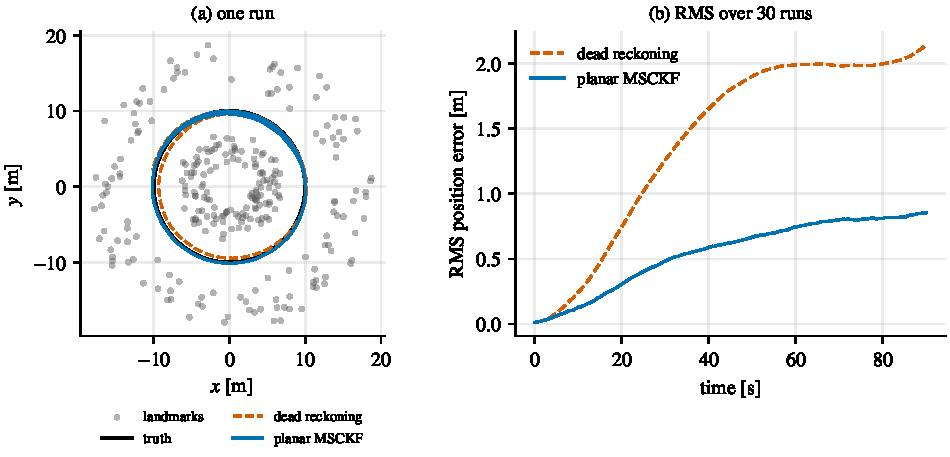
\includegraphics[width=\linewidth]{fig_planar_traj.pdf}
\caption{Planar MSCKF versus dead reckoning. (a) One run. (b) Root-mean-square position error over 30 Monte Carlo runs: after
\SI{90}{s}, \SI{0.85}{m} for the MSCKF against \SI{2.1}{m} for odometry alone.}
\label{fig:planar-traj}
\end{figure}

\begin{figure}[t]
\centering
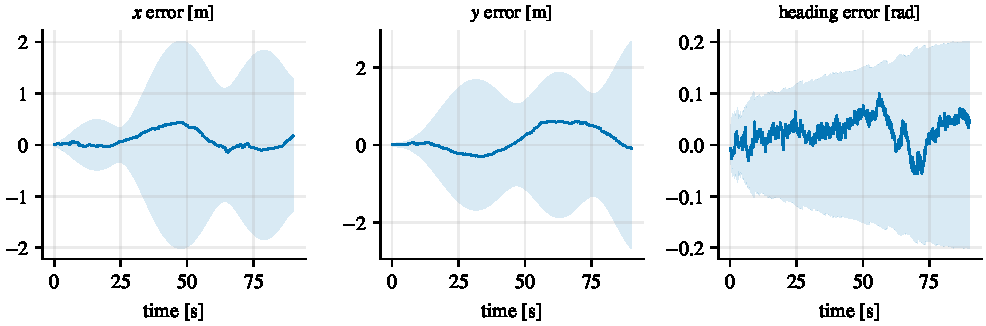
\includegraphics[width=\linewidth]{fig_planar_err.pdf}
\caption{Estimation errors of one run with the filter's $\pm3\sigma$ envelopes (shaded). The position envelopes oscillate because most of the position
uncertainty is perpendicular to the direction of travel, which rotates as the robot circles.}
\label{fig:planar-err}
\end{figure}

\begin{figure}[t]
\centering
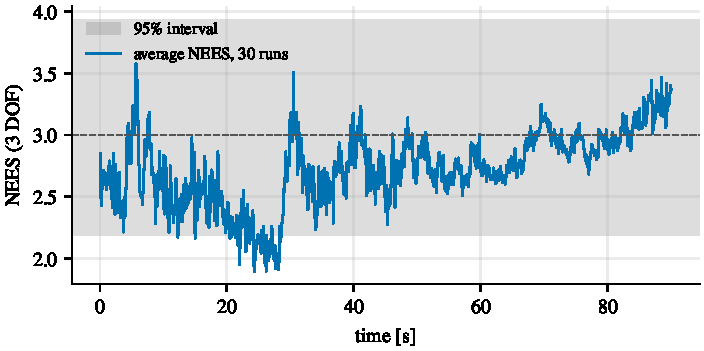
\includegraphics[width=0.8\linewidth]{fig_planar_nees.pdf}
\caption{Average NEES of the robot pose over 30 runs, with the 95\% acceptance interval of \cref{eq:anees-bounds}.}
\label{fig:planar-nees}
\end{figure}

The results (\cref{fig:planar-traj,fig:planar-err,fig:planar-nees}) illustrate four points.
\begin{enumerate}
  \item \textbf{The camera helps, mostly through the heading.} Odometry alone accumulates a heading error with standard deviation
        $\sigma_\omega\sqrt{t} = \SI{0.19}{rad}$ after \SI{90}{s}. The MSCKF ends at about \SI{0.07}{rad}: the camera measures the relative rotation between clones far
        better than the gyro-like turn rate, and because heading errors turn into cross-track position errors, the position error drops by a
        factor of 2.5.
  \item \textbf{The error still grows.} Even with the camera, the heading and position uncertainties grow without bound (\cref{fig:planar-err}).
        This is not a failure: global position and heading are unobservable (\cref{sec:planar-unobservable}), and an odometry filter without loop
        closures can only slow their drift, never stop it. The along-track error is set by the odometry speed noise alone, since a monocular camera
        cannot measure scale (the worked example above).
  \item \textbf{The filter is consistent.} The errors stay inside their $3\sigma$ envelopes, and the average NEES stays inside its acceptance
        interval, apart from mildly conservative dips below it between about 12 and \SI{28}{s}. The gate rejected 5.2\% of the features, close to the 5\% that a $\chi^2_{0.95}$ gate should reject when the filter is
        consistent and every feature is a good one; a much larger rate would signal an overconfident filter or bad data.
  \item \textbf{But the NEES creeps upward.} In the second half of the run its 15-second averages rise steadily, from 2.75 to 2.86 to 3.05, with peaks near 3.5. It is still inside the
        interval, but the trend is systematic: the filter is beginning to believe it knows the heading better than it does. The mechanism, and its cure, are the subject of \cref{ch:observability}.
\end{enumerate}

% ------------------------------------------------------------------------------
\section{The unobservable directions}
\label{sec:planar-unobservable}
\index{unobservable directions!planar}

Suppose we rotate the entire world, the trajectory and every feature, about the origin by a small angle, or translate it. Odometry measures
speed and turn rate in the body frame and does not notice. The camera measures bearings relative to the robot and does not notice either. No
sensor can therefore distinguish the true world from the rotated or translated one: these three directions are \emph{unobservable}
(\cref{sec:observability-linear}), and the filter should never gain information along them.

In error-state coordinates the three directions are the columns of
\begin{equation}
  N = \begin{bmatrix} N_t & N_r \end{bmatrix}, \qquad
  N_t = \begin{bmatrix} I_2 \\ 0 \\ I_2 \\ 0 \\ \vdots \end{bmatrix}, \qquad
  N_r = \begin{bmatrix} \Omega\hat p \\ 1 \\ \Omega\hat p_1 \\ 1 \\ \vdots \end{bmatrix},
  \label{eq:planar-nullspace}
\end{equation}
with one block pair for the robot and one for each clone. $N_t$ shifts every position by the same vector. $N_r$ is the derivative of a rotation
about the origin: a point $p$ moves by $\delta\,\Omega p$, and every heading increases by $\delta$.

\begin{proposition}[The planar nullspace]
\label{prop:planar-nullspace}
If all Jacobians are evaluated at one common set of estimates, then:
\begin{enumerate}
  \item every feature Jacobian satisfies $H_{x,j}N_t + H_{f,j} = 0$ and $H_{x,j}N_r + H_{f,j}\,\Omega\hat p_f = 0$, and therefore the projected Jacobian
        satisfies $H_{o,j}N = 0$;
  \item the exact transition \eqref{eq:planar-phi} maps the nullspace at step $k$ to the nullspace at step $k+1$, $\Phi_kN(\hat x_k) = N(\hat x_{k+1})$;
  \item cloning maps $N$ to the nullspace of the augmented state, $JN = N_{\text{aug}}$.
\end{enumerate}
\end{proposition}
\begin{proof}
(1) Row $i$, translation: $-J_\pi R_i\T + J_\pi R_i\T = 0$. Rotation: using $R_i\T\Omega = \Omega R_i\T$ (\cref{lem:omega}(3)),
\begin{equation*}
  -J_\pi R_i\T\Omega\hat p_i - J_\pi\Omega\hat p_{b,i} + J_\pi R_i\T\Omega\hat p_f = J_\pi\big(\Omega R_i\T(\hat p_f - \hat p_i) - \Omega\hat p_{b,i}\big) = J_\pi(\Omega\hat p_{b,i} - \Omega\hat p_{b,i}) = 0 .
\end{equation*}
Multiplying by $A_j\T$ and using $A_j\T H_{f,j} = 0$ gives $A_j\T H_{x,j}N = 0$.
(2) On the robot block, $\Phi_k(I_2, 0) = (I_2, 0)$, and $\Phi_k(\Omega\hat p_k, 1) = (\Omega\hat p_k + \Omega(\hat p_{k+1} - \hat p_k), 1) = (\Omega\hat p_{k+1}, 1)$; clone blocks are untouched.
(3) The new clone copies the robot's rows of $N$, which are exactly the rows a clone at $\hat p$ should have.
\end{proof}

In words: the linearized filter has the same three unobservable directions as the real system, \emph{as long as every Jacobian uses the same
estimate of each quantity}. A real filter cannot honour this condition. The transition $\Phi_k$ uses $\hat p_{k+1} - \hat p_k$ computed from the
estimate before the update at step $k+1$, while the next transition starts from the corrected estimate; and a clone is linearized at its
current, corrected estimate, not at the value it had when it was created. The identities of \cref{prop:planar-nullspace} then hold only
approximately, the linearized system has an observable heading that the real system does not, and the filter slowly gains spurious heading
information. That is the upward creep in \cref{fig:planar-nees}. \Cref{ch:observability} analyses it in the planar EKF-SLAM setting, where it is most
visible, and shows how First-Estimates Jacobians restore the nullspace.

% ------------------------------------------------------------------------------
\section{From the plane to three dimensions}
\label{sec:planar-to-3d}

\Cref{tab:planar-to-3d} lists every difference between the planar filter and the project's filter. None of them changes the structure of
\cref{alg:planar-msckf}; each changes a formula inside it.

\begin{table}[t]
\centering
\small
\caption{The planar MSCKF and its three-dimensional counterpart.}
\label{tab:planar-to-3d}
\begin{tabularx}{\linewidth}{@{}>{\raggedright\arraybackslash}p{0.2\linewidth}>{\raggedright\arraybackslash}X>{\raggedright\arraybackslash}X@{}}
\toprule
& Plane & Project (AGENTS.md) \\
\midrule
Attitude & heading $\psi$, $R(\psi) = \exp(\psi\Omega)$ & $q_{wb}$, $R_{wb}$, $\Exp$ (\cref{ch:lie}) \\
Error and retraction & $\delta\psi = \psi - \hat\psi$; local and global coincide & local (right) perturbation $q = \hat q\otimes\Exp_q(\delta\theta)$ (C4) \\
Skew operator & $\Omega$, commutes with every $R(\psi)$ & $\sx{\cdot}$; $R\sx{v}R\T = \sx{Rv}$, no commutation \\
Jacobian of $R\T a$ w.r.t.\ the rotation error & $-\Omega R\T a$ & the inverse-action row of \cref{tab:jacobians} \\
Motion sensor & odometry $(v, \omega)$, no biases & IMU $(a_m, \omega_m)$ with gravity and biases (C6) \\
State & $(p, \psi)$ + clones, $3 + 3N$ & $(p, v, q, b_a, b_g)$ + clones, $15 + 6N$ (C3) \\
Camera & 1D bearing $z = y/x$ & 2D normalized $(x/z, y/z)$, through $T_{bc}$ (C6) \\
Constraints per feature & $M - 2$ & $2M - 3$ \\
Reset Jacobian & $1$ & $I - \tfrac12\sx{\delta\hat\theta}$ per attitude (F4) \\
Unobservable directions & 2 translations + heading & 3 translations + yaw (roll and pitch are observable through gravity) \\
\bottomrule
\end{tabularx}
\end{table}

\begin{takeaways}
\begin{itemize}
  \item In the plane every MSCKF Jacobian takes a line: $\partial z/\partial\delta\psi_i = -(1 + z^2)$, $\partial z/\partial\delta p_i = -J_\pi R_i\T$, $H_f = J_\pi R_i\T$.
  \item A camera measures rotation independently of depth, and translation only through parallax ($1/x$).
  \item A feature seen $M$ times gives $M - 2$ constraints in the plane ($2M - 3$ in space); for three views the constraint is a second difference
        that measures the ratio of baselines and the relative headings, but not scale, global position or global heading.
  \item The planar filter is consistent and reduces the dead-reckoning error by a factor of about 2.5, yet its NEES creeps upward: the first sign
        of the spurious heading information studied in \cref{ch:observability}.
  \item The step to three dimensions changes formulas, not structure: non-commuting rotations, the local perturbation, gravity, biases and the reset Jacobian.
\end{itemize}
\end{takeaways}

\begin{exercises}
  \item Verify \cref{prop:planar-H} by finite differences at a random clone pose and feature. Then explain $\partial z/\partial\delta\psi = -(1 + z^2)$ using
        only the bearing angle $\beta = \arctan z$.
  \item Show that $I + F_c\Dt$ and the exact $\Phi_k$ of \eqref{eq:planar-phi} differ by $O(\Dt^2)$, and identify the term.
  \item Add a turn-rate bias $b_\omega$ ($\omega_m = \omega + b_\omega + n_\omega$, $\dot b_\omega = n_b$) to the planar state. Derive the new column of $F_c$ and the new
        row of $G_c$, and show that the bias is observable once the camera sees features. Compare with the gyroscope-bias block of the
        three-dimensional filter.
  \item Repeat the worked example with unequal baselines, $\hat p_3 = (0, 2)$. Find $a$, and show that the projected residual measures the
        ratio of the two baselines.
  \item In the worked example, show that moving the \emph{middle} clone along the viewing direction $x_w$ is invisible to $H_o$, while moving the
        \emph{first} clone along $x_w$ is visible. Interpret the difference in terms of the bearing each clone has to the feature.
  \item Why does a 1D camera need three views of a feature to say anything about the poses, while a 2D camera needs only two? Relate the answer
        to the dimensions of $H_f$.
  \item Run \code{scripts/planar\_sims.py} with window sizes $N_{\max} = 3, 5, 10, 20$ and plot the final RMS position error. Explain the trend, and what
        limits the benefit of a longer window.
  \item Prove part (1) of \cref{prop:planar-nullspace} without using the closed-form Jacobians: argue directly that a measurement function that depends only
        on $R(\psi_i)\T(p_f - p_i)$ cannot change under a common rotation or translation of all positions.
  \item Replace the bearing camera by a range-and-bearing sensor. How many constraints does a feature seen $M$ times give? Which of the unobservable
        directions of \eqref{eq:planar-nullspace} become observable, if any?
\end{exercises}
% Solutions to the exercises of Chapter 27.
\begin{solutions}
  \item At a random clone pose and a feature with $\hat z = 0.3$, central differences with $\varepsilon = 10^{-6}$ agree with \eqref{eq:planar-H} to $10^{-10}$ in all five entries. For the
        heading entry, $\beta = \arctan z$ is the angle between the body axis $x_b$ and the ray to the feature. Turning the robot left by $\delta\psi$ turns the body axis
        toward the ray, so every bearing \emph{decreases} by exactly $\delta\psi$, whatever the depth: $\delta\beta = -\delta\psi$. Since $z = \tan\beta$,
        \[
          \frac{\partial z}{\partial\delta\psi} = \frac{\dd z}{\dd\beta}\,\frac{\partial\beta}{\partial\delta\psi} = \frac{1}{\cos^2\beta}\,(-1) = -(1 + \tan^2\beta) = -(1 + z^2).
        \]
        The factor $1 + z^2$ only converts angle to normalized coordinate: at the edge of the $\pm50^\circ$ field of view it is $2.4$, while in angle every point moves
        by the same $\delta\psi$.

  \item The top-right block of $I + F_c\Dt$ is $\Omega R(\hat\psi_k)e_1v_m\Dt$, while that of $\Phi_k$ is $\Omega(\hat p_{k+1} - \hat p_k) = \Omega R(\hat\psi_k + \tfrac12\omega_m\Dt)e_1v_m\Dt$. With
        $R(\hat\psi_k + \tfrac12\omega_m\Dt) = R(\hat\psi_k)(I + \tfrac12\omega_m\Dt\,\Omega) + O(\Dt^2)$ and $\Omega^2 = -I$,
        \[
          \Phi_k - (I + F_c\Dt) = \begin{bmatrix} 0 & -\tfrac12v_m\omega_m\Dt^2\,R(\hat\psi_k)e_1 \\ 0 & 0\end{bmatrix} + O(\Dt^3).
        \]
        The term is $\tfrac12\Dt^2\,\Omega\ddot{\hat p}$: the nominal path turns during the step, so its displacement is not $\dot{\hat p}_k\Dt$. Note that $F_c^2 = 0$, so for a
        \emph{constant} $F_c$ the matrix exponential would add nothing. The whole difference comes from $F_c$ changing during the step: $I + F_c\Dt$ is the rectangle rule for
        $I + \int F_c\,\dd t$. For the simulation ($v = 1$~m/s, $\omega = 0.1$~rad/s, $\Dt = 0.01$~s) it is $5\times10^{-6}$ per step, relative size $\tfrac12\omega\Dt = 5\times10^{-4}$. It is small,
        but it means the approximate transitions no longer telescope exactly into $\Omega(\hat p_k - \hat p_0)$ (\cref{ch:observability}).

  \item With $\omega = \omega_m - b_\omega - n_\omega$ and the nominal $\dot{\hat\psi} = \omega_m - \hat b_\omega$, $\dot{\delta\psi} = -\delta b_\omega - n_\omega$ and $\dot{\delta b}_\omega = n_b$; the position row is unchanged. For
        $\delta x_R = (\delta p, \delta\psi, \delta b_\omega)$ and $n = (n_v, n_\omega, n_b)$,
        \[
          F_c = \begin{bmatrix} 0_{2\times2} & \Omega R(\hat\psi)e_1v_m & 0_{2\times1} \\ 0 & 0 & -1 \\ 0 & 0 & 0 \end{bmatrix}, \qquad
          G_c = \begin{bmatrix} -R(\hat\psi)e_1 & 0 & 0 \\ 0 & -1 & 0 \\ 0 & 0 & 1 \end{bmatrix},
        \]
        with $Q_c = \diag(\sigma_v^2, \sigma_\omega^2, \sigma_b^2)$: the new column of $F_c$ is $(0, 0, -1, 0)\T$ and the new row of $G_c$ is $(0, 0, 1)$. The camera measures relative headings of
        the clones directly: the heading column $-(1 + z^2)$ does not depend on depth, and turning a single clone is visible. A bias error makes the heading error grow
        linearly across the window, $\delta\psi(t) = \delta\psi_0 - t\,\delta b_\omega$. The unobservable directions cannot produce such a ramp: a global rotation adds the same constant to every
        heading, and translations and scale leave headings unchanged. So the ramp changes the projected residuals, and the bias is observable. Numerically: on
        the simulated circle with ten clones and six landmarks, the observability matrix of $(\delta p, \delta\psi, \delta b_\omega)$ at the first clone time has rank one. Its
        three-dimensional nullspace (the two translations and the rotation) has bias components of $10^{-14}$.
        \ifsolutions
        In three dimensions the attitude row is $\dot{\delta\theta} = -\sx{\hat\omega}\delta\theta - \delta b_g - n_g$ and the bias row $\dot{\delta b}_g = n_{b_g}$. The $-I$ in the gyro-bias columns is the exact
        counterpart of the $-1$ here. The extra term $-\sx{\hat\omega}\delta\theta$ has no planar analog, because a planar heading error does not rotate with the body. For the same
        reason as here, all three gyroscope-bias components are observable once the camera measures relative attitudes: even the bias about the vertical,
        although the global yaw is not.
        \else
        In three dimensions the same mechanism makes all three gyroscope-bias components observable once the camera measures relative attitudes: even the bias
        about the vertical, although the global yaw is not. (The corresponding block of $F_c$ is part of the derivation exercises of \cref{ch:errordyn}.)
        \fi

  \item The body-frame points are $(4, 1)$, $(4, 0)$, $(4, -2)$, so $\hat z = (\tfrac14, 0, -\tfrac12)$ and
        \[
          H_f = \begin{bmatrix} -\tfrac1{16} & \tfrac14 \\ 0 & \tfrac14 \\ \tfrac18 & \tfrac14 \end{bmatrix}, \qquad
          h_1\times h_2 = \tfrac1{64}(-2, 3, -1), \qquad a = \tfrac1{\sqrt{14}}(2, -3, 1),
        \]
        so $r_o = (2r_1 - 3r_2 + r_3)/\sqrt{14}$. For sideways motion at a fixed heading, $z_i = (y_f - y_i)/x_f$ is a linear function of the camera position $y_i = (-1, 0, 2)$, and
        the weights annihilate exactly the constants and the linear functions: $\sum_ia_i = 0$ and $\sum_ia_iy_i = 0$. For baselines $b_1 = y_2 - y_1$ and $b_2 = y_3 - y_2$, the weights are
        $(b_2, -(b_1 + b_2), b_1)$, and $r_o = 0$ exactly when
        \[
          \frac{z_1 - z_2}{z_2 - z_3} = \frac{b_1}{b_2} .
        \]
        The depth $x_f$ cancels in the ratio of image displacements, so the residual compares the observed ratio with the estimated ratio of the baselines, and
        nothing else. If the middle clone were really at $y = 0.1$, the observed ratio would be $1.1/1.9 = 0.58$ instead of $\tfrac12$, and $r_o = -0.020$. The projected Jacobian
        is $H_o = \tfrac1{\sqrt{14}}\big[(\tfrac18, -\tfrac12, -\tfrac{17}8)\ \ (0, \tfrac34, 3)\ \ (-\tfrac18, -\tfrac14, -\tfrac54)\big]$; translation, rotation and scale of the configuration give zero, as before.

  \item With $a = (1, -2, 1)/\sqrt6$, the $\delta p_x$ entries of $H_o$ are $\tfrac{1}{16\sqrt6}$, $0$ and $-\tfrac{1}{16\sqrt6}$. Moving the middle clone along $x_w$ is invisible; moving the first clone
        along $x_w$ is visible, though weakly. The middle clone looks straight at the feature ($\hat z_2 = 0$), so $x_w$ is its own viewing ray, the nullspace of its projection
        Jacobian: moving along the ray changes the depth, which one view cannot see, and leaves the bearing unchanged. The first clone sees the feature at
        $\hat z_1 = \tfrac14$ ($14^\circ$). Moving it along $x_w$ changes that bearing by $\tfrac{1}{16}$ per meter, and the feature cannot absorb the change without disturbing the other two bearings. In
        general, moving a clone along its ray to a feature is invisible in that feature's residual. Other directions are visible, with a sensitivity
        proportional to the sine of the angle between motion and ray, divided by the depth.

  \item Each observation gives as many numbers as the image has dimensions, and the feature has as many unknowns as the space. A 1D camera in the plane: $H_{f,j}$ is
        $M\times2$ of rank 2, leaving $M - 2$ constraints, so $M = 2$ gives none. Two rays in a plane always intersect (unless parallel), so any two bearings are consistent with some
        feature. A 2D camera in space: $H_{f,j}$ is $2M\times3$ of rank 3, leaving $2M - 3$, so $M = 2$ gives one. Two rays in space are generically skew, and requiring them to intersect,
        i.e.\ to be coplanar with the baseline, is the epipolar constraint (Exercise~26.3).

  \item Final RMS errors after 90~s over 30 runs (dead reckoning: $2.80$~m):
        \begin{center}\small
        \begin{tabular}{@{}l c c c c@{}}
        \toprule
        $N_{\max}$ (window length) & 3 (0.3~s) & 5 (0.5~s) & 10 (1~s) & 20 (2~s) \\
        \midrule
        position & 2.23~m & 2.13~m & 0.85~m & 0.33~m \\
        heading & 0.19~rad & 0.17~rad & 0.069~rad & 0.025~rad \\
        average NEES (last 9~s, 3 DOF) & 2.65 & 2.97 & 3.14 & 3.20 \\
        \bottomrule
        \end{tabular}
        \end{center}
        The position error follows the heading error, which turns into cross-track error. The key quantity is how well one window determines the heading
        change across it, a heading ramp, which the camera sees only through parallax. With the scenario's landmarks, a single window determines it with a
        standard deviation of $0.05$, $0.022$, $0.008$ and $0.003$~rad for $N_{\max} = 3$, 5, 10, 20. Odometry alone has $\sigma_\omega\sqrt T = 0.009$, $0.013$, $0.019$ and $0.028$~rad over the same spans.
        Short windows are worse than odometry at exactly the quantity that drives the drift; the camera wins only for windows longer than about half a second,
        which is where the error drops. The benefit then levels off: $0.18$~m at $N_{\max} = 40$ and $0.17$~m at 80. Several things limit it:
        \begin{itemize}
          \item once the window pins the heading change far better than odometry, the remaining error is the unobservable drift of global heading and
                position, which no window removes;
          \item tracks end (here a landmark stays in view for a median of 6.8~s), so a longer window cannot lengthen them;
          \item the cost grows as $n^3$ with $n = 3 + 3N_{\max}$;
          \item old clones are never relinearized;
          \item the NEES creeps upward ($3.24$ at $N_{\max} = 80$), as more constraints feed more spurious heading information (\cref{ch:observability}).
        \end{itemize}

  \item Let $h(x, p_f) = \pi\big(R(\psi_i)\T(p_f - p_i)\big)$, or any function of $R(\psi_i)\T(p_f - p_i)$. Translating everything by $t$ ($p_i \to p_i + t$, $p_f \to p_f + t$) leaves $p_f - p_i$ unchanged.
        Rotating everything about the origin by $\delta$ ($p_i \to R(\delta)p_i$, $\psi_i \to \psi_i + \delta$, $p_f \to R(\delta)p_f$) gives
        $R(\psi_i + \delta)\T R(\delta)(p_f - p_i) = R(\psi_i)\T R(\delta)\T R(\delta)(p_f - p_i) = R(\psi_i)\T(p_f - p_i)$. So $h$ is constant along both families, identically in $t$ and $\delta$.
        Differentiating at $t = 0$ and $\delta = 0$, at the common linearization point $(\hat x, \hat p_f)$: the state moves along $N_t$ and the feature by $I$, or the state along $N_r$ and the
        feature by $\Omega\hat p_f$. Hence
        \[
          H_{x,j}N_t + H_{f,j} = 0, \qquad H_{x,j}N_r + H_{f,j}\,\Omega\hat p_f = 0,
        \]
        and multiplying by $A_j\T$ gives $H_{o,j}N = 0$. Nothing about $\pi$ was used. The proof also shows why the hypothesis matters: the identities come from differentiating one
        function at one point, so they hold only if every block of $H_{x,j}$ and $H_{f,j}$ is evaluated at the same estimates.

  \item Each observation $(\|d_i\|, \atantwo(d_y, d_x))$ now gives two numbers for two unknowns of the feature, so a feature seen $M$ times gives $2M - 2$ constraints. A single
        observation determines the feature and constrains nothing; two observations already give two constraints. None of the directions of
        \eqref{eq:planar-nullspace} becomes observable: the measurement is still a function of $R(\psi_i)\T(p_f - p_i)$ alone, so the argument of Exercise~8 applies unchanged, and global
        translation and heading remain invisible. What changes is scale. The range measures distances, so the shape \emph{and size} of the trajectory are now
        observable from the camera alone, and the along-track error no longer depends on the odometry speed noise only.
\end{solutions}


\chapter{The Complete Algorithm}
\label{ch:fullalgo}

\begin{objectives}
\begin{itemize}
  \item Assemble every component into one event-driven estimator, with the correct order of operations.
  \item Estimate the computational budget and map the algorithm onto the project's software architecture.
  \item Diagnose the most common failures from their symptoms.
\end{itemize}
\end{objectives}

% ------------------------------------------------------------------------------
\section{The event loop}

The estimator consumes a single, time-ordered stream of sensor events. Milestone 3 builds it by merging the presorted IMU,
image (and, for testing, pose) arrays with a two-pointer merge, with the rule that an IMU sample precedes any other event
with the same timestamp. \Cref{alg:msckf} shows the loop.

\begin{algorithm}[t]
\caption{Monocular MSCKF}
\label{alg:msckf}
\begin{algorithmic}[1]
\Require event stream, calibration, noise parameters
\LineComment{load phase: allocation allowed}
\State parse data and calibration; build the event arrays; construct the filter and front end with fixed-max workspaces
\State initialize $(\hat x, P)$ (ground truth in the project, logged; static initialization otherwise)
\LineComment{streaming phase: no allocation in the core}
\For{each event $e$ in timestamp order}
  \If{$e$ is an IMU sample at $t$}
    \State propagate nominal state and covariance from $t_{prev}$ to $t$ \Comment{\cref{ch:strapdown,ch:errordyn}}
  \ElsIf{$e$ is an image at $t_c$}
    \State propagate to $t_c$ (interpolated IMU) \Comment{exact image time}
    \State front end: track, verify, undistort; update track histories \Comment{\cref{ch:frontend}}
    \State process tracks that were lost in this image \Comment{\cref{alg:msckf-update}}
    \If{$N = $ \code{kMaxClones}}
      \State process tracks with an observation at the oldest clone
      \State marginalize the oldest clone in place \Comment{\cref{ch:cloning}}
    \EndIf
    \State clone $(\hat p, \hat q)$; $P \gets JPJ\T$; attach this image's observations to the new clone
  \EndIf
  \State log state, $\diag(P)$, NIS and gate statistics to the preallocated buffer
\EndFor
\end{algorithmic}
\end{algorithm}

Three ordering rules are essential.
\begin{enumerate}
  \item \textbf{Propagate before you update.} A measurement at time $t$ must be applied to the state at time $t$, never to the
        state at the previous IMU sample.
  \item \textbf{Use a clone's observations before you delete it.} Every feature with an observation at the oldest clone is
        processed before that clone is marginalized; otherwise its information is lost.
  \item \textbf{Use each observation once.} After a track has been used, its observations are discarded. If the feature keeps
        being tracked, later observations form a new track.
\end{enumerate}
With the order of \cref{alg:msckf}, the window never holds more than \code{kMaxClones} clones, which keeps the covariance within its
fixed maximum size. A feature processed because its oldest clone is leaving cannot use the current image's observation in that
update, because the new clone does not exist yet. Implementations that clone first need room for one extra clone. Either
choice is valid; the storage bound must match it.
The planar filter of \cref{ch:planar} runs exactly this loop (\cref{alg:planar-msckf}) in a few lines of Python, which makes it a
convenient place to experiment with the ordering rules before committing to them in C++.

\begin{figure}[t]
\centering
\begin{tikzpicture}[xscale=0.9, yscale=1.0]
  \draw[->, thick] (0,0) -- (15.5,0) node[right, font=\footnotesize] {$t$};
  \foreach \x in {0,0.25,...,15.0} \draw[black!45] (\x,-0.08) -- (\x,0.08);
  \node[font=\scriptsize, black!60, below] at (0.6,-0.15) {IMU, 200 Hz};
  \foreach \k/\x in {1/1.25, 2/3.75, 3/6.25, 4/8.75, 5/11.25, 6/13.75} {
    \draw[primary, thick] (\x,-0.25) -- (\x,0.6);
    \draw[fill=primarylight, draw=primary] (\x-0.25,0.6) rectangle (\x+0.25,1.0);
    \node[font=\scriptsize] at (\x,0.8) {$C_\k$};
  }
  \node[font=\scriptsize, primary, below] at (3.75,-0.25) {image (20 Hz)};
  % features
  \draw[plotgreen, very thick] (1.25,1.35) -- (8.75,1.35) node[right, font=\scriptsize] {track $f_1$ lost $\Rightarrow$ update};
  \fill[plotgreen] (1.25,1.35) circle (2pt) (3.75,1.35) circle (2pt) (6.25,1.35) circle (2pt) (8.75,1.35) circle (2pt);
  \draw[plotorange, very thick] (3.75,1.85) -- (13.75,1.85);
  \fill[plotorange] (3.75,1.85) circle (2pt) (6.25,1.85) circle (2pt) (8.75,1.85) circle (2pt) (11.25,1.85) circle (2pt) (13.75,1.85) circle (2pt);
  \node[font=\scriptsize, plotorange, align=left, right] at (13.85,1.95) {$f_2$: oldest clone\\leaving $\Rightarrow$ update};
  \draw[decorate, decoration={brace, amplitude=4pt}] (3.5,2.25) -- (14.0,2.25) node[midway, above=5pt, font=\scriptsize] {window (example \code{kMaxClones} = 5)};
  \draw[conv, ->] (1.25,2.5) -- (1.25,1.1) node[pos=0, above, font=\scriptsize, align=center] {$C_1$ marginalized\\when $C_6$ arrives};
\end{tikzpicture}
\caption{Timeline of the MSCKF. The IMU propagates at 200~Hz; each image creates a clone; feature tracks are processed when
they end or when the clone holding their oldest observation is about to leave the window.}
\label{fig:timeline}
\end{figure}

% ------------------------------------------------------------------------------
\section{Initialization and the first seconds}

The project initializes from ground truth, which removes the hardest failure mode from early testing and is logged as a use of
ground truth (Milestone 10b). With static initialization (\cref{ch:strapdown}), the first seconds are delicate: the yaw is
arbitrary, the accelerometer bias is entangled with tilt, and the window contains few clones with little parallax. Generous
initial covariances, and a check that enough features with sufficient parallax exist before trusting visual updates, avoid
early divergence. Inspect the IMU data of each EuRoC sequence before running on it: a static start followed by vigorous
motion is the easiest case for initialization, and a fast start the hardest.

% ------------------------------------------------------------------------------
\section{Computational budget}

With $N = 10$ clones the error state has $n = 75$ dimensions. Rough flop counts per operation:
\begin{center}\small
\begin{tabular}{@{}l l r@{}}
\toprule
Operation & Frequency & Cost (flops) \\
\midrule
Nominal propagation & 200 Hz & $\sim10^2$ \\
$P_{II}$, $P_{IC}$ propagation & 200 Hz & $\sim4\times10^4$ \\
Cloning ($P \gets JPJ\T$ as block copies) & 20 Hz & $\sim10^4$ \\
Per feature: triangulation, projection, gating ($M = 6$) & per track & $\sim10^5$ \\
QR compression of $d = 450$ rows & per update & $\sim5\times10^6$ \\
Update ($S$, gain, Joseph) with $n = 75$ & per update & $\sim6\times10^6$ \\
Front end (KLT on 150 features) & 20 Hz & dominant in time \\
\bottomrule
\end{tabular}
\end{center}
The filter core needs on the order of $10^7$ flops per image, a few milliseconds on an embedded processor and well under a
millisecond on a desktop. The front end is usually the bottleneck in wall-clock time. The cubic growth with $n$ is why the window
is short and why QR compression matters for large stacks.

% ------------------------------------------------------------------------------
\section{Software architecture}

\begin{figure}[t]
\centering
\begin{tikzpicture}[node distance=8mm and 10mm]
  \node[block, minimum width=48mm, align=left] (core) {\textbf{vio\_core} (static, Eigen only)\\ \footnotesize so3, imu\_integrator, es\_ekf,\\ \footnotesize camera\_model, triangulation, msckf\_update};
  \node[block, minimum width=34mm, above left=10mm and -14mm of core, align=left] (io) {\textbf{vio\_io}\\ \footnotesize dataset\_loader, telemetry\\ \footnotesize + YAML parser};
  \node[block, minimum width=34mm, above right=10mm and -14mm of core, align=left] (fe) {\textbf{vio\_frontend}\\ \footnotesize visual\_frontend\\ \footnotesize + OpenCV};
  \node[block, minimum width=30mm, above=24mm of core, fill=white] (app) {\textbf{vio\_app}\\ \footnotesize main.cpp};
  \draw[->, thick] (io) -- (core); \draw[->, thick] (fe) -- (core);
  \draw[->, thick] (app) -- (io); \draw[->, thick] (app) -- (fe); \draw[->, thick] (app) -- (core);
  \node[font=\footnotesize, align=center, below=2mm of core] {arrows: ``depends on''. OpenCV never reaches \code{vio\_core};\\ each test links only the library it tests.};
\end{tikzpicture}
\caption{Library targets of the project (AGENTS.md). Dependencies point one way, so the estimator core can be built, tested and
reasoned about without the I/O and vision libraries.}
\label{fig:architecture}
\end{figure}

\Cref{fig:architecture} shows how the algorithm maps to the project's targets. The zero-allocation discipline applies to
\code{vio\_core}, which contains everything executed per IMU sample and per update. The front end may allocate but must reuse its
buffers, and the I/O layer allocates freely during loading.

% ------------------------------------------------------------------------------
\section{Debugging guide}

\begin{table}[t]
\centering\small
\begin{tabularx}{\textwidth}{@{}>{\raggedright\arraybackslash}p{4.4cm} X@{}}
\toprule
\textbf{Symptom} & \textbf{Likely causes} \\
\midrule
Altitude diverges at about $2g$ in IMU-only propagation & gravity or specific-force sign; $g_w$ added twice \\
Position diverges within seconds even with ground-truth init & $R_{wb}$ used as $R_{bw}$; quaternion $w/z$ swapped at load; gyro and accel columns or biases swapped; degrees vs radians \\
Rotation matrices slowly scale vectors & missing quaternion normalization \\
NaN after a while & missing Taylor branch; $\Log$ near $\pi$; $\Jrinv$ evaluated beyond $\pi$; feature at zero depth; Cholesky of a non-PD $S$ \\
Corrections systematically make things worse & sign of $H$ or of the residual; injection on the wrong side of the quaternion; global vs local convention mixed \\
Covariance loses symmetry or positive definiteness & simple update form instead of Joseph; missing symmetrization; aliasing in Eigen block products \\
Nearly all features fail the gate & overconfident $P$; $T_{bc}$ inverted; pixel noise used in normalized units (or vice versa); distortion not removed; timestamps misaligned \\
Gate rejects nothing & $R_z$ or $\sigma_{uv}$ far too large; gate threshold indexed with the wrong dimension \\
Slowly growing yaw error with healthy NIS & expected EKF inconsistency along unobservable yaw (\cref{ch:observability}) \\
Scale drift & little acceleration (degenerate motion); accelerometer noise or bias badly tuned \\
Works on synthetic data, fails on EuRoC & extrinsics, time offset, distortion, noise inflation, initialization, IMU gaps \\
Results differ between runs & uninitialized memory (run the sanitizers); unseeded random generators \\
\bottomrule
\end{tabularx}
\caption{Symptoms and their most frequent causes.}
\label{tab:debugging}
\end{table}

\Cref{tab:debugging} collects the failures that experience shows are most common. The milestone structure of the project is itself
the most effective debugging tool: each layer is verified against known truth before the next is built on top of it, so a new
failure is almost always in the newest layer.

\section{What to expect on EuRoC}

Published monocular filter-based estimators reach absolute trajectory errors of the order of 0.1 to 0.5~m on the machine-hall
sequences, depending on features, tuning and initialization, with the difficult sequences (fast motion, motion blur, dark
regions) considerably worse~\cite{delmerico2018benchmark}. Milestone 10b sets a first-pass target of 0.5~m on MH\_01 and a stretch target of
0.2~m. Yaw and position drift without bound; roll and pitch remain accurate throughout; velocity and biases converge within the
first seconds of excitation.

\begin{takeaways}
\begin{itemize}
  \item One time-ordered stream; propagate to each event's time before applying it.
  \item At each image: process lost tracks; if the window is full, process the oldest clone's tracks and marginalize it; then clone.
  \item The core costs about $10^7$ flops per image; the front end usually dominates the run time.
  \item Dependencies point one way: \code{vio\_core} knows nothing about files, YAML or OpenCV.
  \item Most failures map to a small set of sign, frame, unit and timing errors; test each layer against truth.
\end{itemize}
\end{takeaways}

\begin{exercises}
  \item Write the event-loop pseudocode for the alternative ordering (clone first, then process and marginalize). What capacity
        does it require, and what does it gain?
  \item Instrument a run to record the number of features processed per update, their observation counts, and the stacked row
        count $d$. Choose the compile-time row cap from the distribution.
  \item For each row of \cref{tab:debugging}, design a unit or integration test that would have caught the cause before the full
        system was assembled.
\end{exercises}
% Solutions to the exercises of Chapter 28.
\begin{solutions}
  \item With the clone created first, an image at $t_c$ is handled as follows:
        \begin{enumerate}[label=\arabic*:, leftmargin=2.2em, itemsep=0pt]
          \item propagate to $t_c$; run the front end;
          \item clone $(\hat p, \hat q)$; $P \gets JPJ\T$; attach this image's observations to the new clone (now $N + 1$ clones);
          \item process the tracks lost in this image;
          \item \textbf{if} $N + 1 > $ \code{kMaxClones}: process the tracks with an observation at the oldest clone (including the current observation), then
                marginalize the oldest clone.
        \end{enumerate}
        The window transiently holds \code{kMaxClones}$\,+\,1$ clones, so every fixed-max buffer ($P$, the stacked $H$, the clone container) must be sized for
        $15 + 6(\text{\code{kMaxClones}} + 1)$ states. The gain: a track processed because its oldest clone is leaving can include the current image's observation. That is
        its newest view and usually the one with the most parallax relative to the oldest, so it adds two rows per track and lengthens the baseline. The price
        is an update on a state six dimensions larger, about $(81/75)^3 \approx 1.26$ times the cost for \code{kMaxClones}$\,= 10$.

  \item Log, for every update, the number of features processed, each feature's $M_j$, and $d = \sum_j(2M_j - 3)$, and plot the distribution over all sequences. The
        planar filter of \cref{ch:planar} ($N_{\max} = 10$, 4\,500 updates) shows the typical shape. On average 2.4 features are processed per update. Most tracks reach the full
        window ($M = 10$ for 90\% of them), because they are processed when their oldest clone leaves. The rows per update have median 16 and 99th percentile 56,
        but the maximum is 175. The tail comes from bursts: when the window first fills, or when many features leave the view together, nearly every visible
        feature is processed at once. The worst case is therefore (visible features)$\,\times\,$(rows per full track): $150\times(2\cdot10 - 3) = 2550$ rows for the
        project. There are two sound ways to set the cap:
        \begin{itemize}
          \item size the workspace for the worst case: $2550\times76$ doubles are 1.5~MB, allocated once at load time;
          \item better, compress incrementally: append features until the next one would not fit, QR-compress the stack to $n$ rows
                (\cref{prop:compression}), and continue. The workspace then needs only $n$ plus one feature's rows ($75 + 17$), and no feature is ever dropped.
        \end{itemize}
        A cap at a percentile of the distribution without either measure would silently discard information in exactly the bursts that matter. If it is used,
        the dropped features must be counted and logged.

  \item One test per row of \cref{tab:debugging}:
        \begin{itemize}
          \item \emph{$2g$ altitude divergence:} propagate a level, stationary IMU ($a_m = (0, 0, 9.81)$, $\omega_m = 0$) for 10~s from rest; position and velocity must stay
                zero to rounding. Then propagate free fall ($a_m = 0$) and require $v_z = -9.81\,t$.
          \item \emph{Divergence within seconds:} loader tests on a fixture row with distinct values in every column (catching $w$/$z$ swaps, gyro/accel and bias column
                order, degrees). A coning test against an analytic attitude. On EuRoC, propagate IMU-only from ground truth for 1~s and compare with ground truth.
          \item \emph{Vectors slowly scaled:} after $10^6$ random multiplicative updates, $\big|\|q\| - 1\big| < 10^{-12}$.
          \item \emph{NaN:} $\Exp$, $\Log$ and $\Jrinv$ at $0$, $10^{-12}$, $\pi - 10^{-9}$ and exactly $\pi$; triangulation must reject zero and negative depths; feeding a non-PD $S$ must return an
                error, not a NaN; a randomized test asserting finite outputs.
          \item \emph{Corrections make things worse:} finite-difference tests of every Jacobian on $\bplus/\bminus$. An update with a noise-free measurement must reduce the
                error. A mutation check: flip a sign in $H$ and confirm the test fails.
          \item \emph{Covariance loses symmetry or definiteness:} after $10^4$ random updates, $\|P - P\T\| < 10^{-12}\|P\|$ and $\lambda_{\min}(P) \ge 0$. Compare in-place block products with an
                out-of-place reference.
          \item \emph{All features gated out:} a synthetic VIO run with the true noise must reject about 5\% of the features (say 3--8\%). A camera-model test projects a hand-computed
                point through $T_{bc}$ from \code{sensor.yaml}. A unit test checks $\sigma_{uv} = \sigma_{px}/f$.
          \item \emph{Gate rejects nothing:} the same run, with a lower bound on the rejection rate; the $\chi^2$ table checked against reference values, indexed by
                $\dim r$.
          \item \emph{Growing yaw error:} per-component NEES on synthetic data; position, roll and pitch must be consistent, and yaw growth is documented as expected.
          \item \emph{Scale drift:} two synthetic runs, with low and high acceleration; the scale error must be bounded in the excited run.
          \item \emph{Synthetic fine, EuRoC fails:} parse the real \code{T\_BS} (row-major) and intrinsics, and compare with hand-copied values; distortion round trip at the corners and
                edges (Exercise~20.5); merge-order test (IMU before image at equal times); IMU-gap detection ($\Dt > 2\times$ nominal flagged).
          \item \emph{Run-to-run differences:} run the pipeline twice in one test and compare outputs bitwise; sanitizers in CI; seeded generators.
        \end{itemize}
\end{solutions}



\part{Beyond the Baseline}
\chapter{Observability and Consistency of VIO}
\label{ch:observability}
\chaptermark{Observability and Consistency} % short running header

\begin{objectives}
\begin{itemize}
  \item Define observability for nonlinear systems, and test it with Lie derivatives.
  \item Prove that VIO has four unobservable directions and write them in the project's error coordinates.
  \item Show, in the planar EKF-SLAM problem where every step can be computed, exactly how the standard EKF acquires spurious information,
        and see it happen in a Monte Carlo simulation.
  \item Prove that First-Estimates Jacobians restore the correct unobservable subspace, and understand the alternatives: the
        observability-constrained EKF, the invariant EKF and robocentric formulations.
  \item Know the degenerate motions that remove further information.
\end{itemize}
\end{objectives}

The planar MSCKF of \cref{ch:planar} was consistent, but its NEES crept upward. This chapter explains the creep. The explanation needs one
new idea, observability, and one careful computation, the observability matrix of a linearized filter. The computation is done in full for
planar EKF-SLAM, the setting in which the effect was first understood~\cite{julier2001counter, bailey2006consistency, huang2010observability},
and then carried over to VIO.

% ------------------------------------------------------------------------------
\section{Observability}

\subsection{Indistinguishable states}

Consider a system $\dot x = f(x, u)$ with output $y = h(x)$. Two initial states $x_0$ and $x_0'$ are \term{indistinguishable} if, for every input
signal $u(\cdot)$, they produce the same output signal $y(\cdot)$. No estimator, however clever, can tell them apart: the data are identical. A
system is \emph{observable} at $x_0$ if no other state is indistinguishable from it. Since estimators work locally, the useful notion is
local: $x_0$ is \termi{locally weakly observable}{observability!local weak} if it can be distinguished, over arbitrarily short time intervals, from
every state in some neighborhood of it.

For linear systems the question is settled by the observability matrix (\cref{thm:obs-rank}). For a time-varying linear system
$\delta x_{k+1} = \Phi_k\delta x_k$, $r_k = H_k\delta x_k$ the same object reads as follows.

\begin{definition}[Observability matrix]
\label{def:obs-matrix}
The observability matrix over steps $1, \dots, k$ is
\begin{equation}
  \mathcal{O} = \begin{bmatrix} H_1 \\ H_2\Phi_1 \\ H_3\Phi_2\Phi_1 \\ \vdots \\ H_k\Phi_{k-1}\cdots\Phi_1 \end{bmatrix}.
\end{equation}
An initial error $\delta x_1 \in \nullsp(\mathcal{O})$ produces no change in any measurement, so it cannot be detected.
$\nullsp(\mathcal{O})$ is the \term{unobservable subspace}.
\end{definition}

A Kalman filter can gain information only in directions outside $\nullsp(\mathcal{O})$. Along unobservable directions its covariance may grow
(from process noise) but must never shrink. This is the property that the standard EKF violates.

\subsection{Nonlinear observability and Lie derivatives}

For a nonlinear system the observability matrix is replaced by derivatives of the output along the dynamics. Suppose the dynamics are
\emph{control-affine}, $\dot x = f_0(x) + \sum_i f_i(x)\,u_i$, as kinematic models usually are (the inputs are the measured rates and
accelerations). The \termi{Lie derivative}{Lie derivative} of a scalar function $\varphi$ along a vector field $f$ is its rate of change along the flow of $f$,
\begin{equation}
  L_f\varphi(x) = \nabla\varphi(x)\cdot f(x),
\end{equation}
and repeated derivatives are written $L_gL_f\varphi = \nabla(L_f\varphi)\cdot g$. Differentiating the output along a trajectory gives
\begin{equation}
  y = h(x), \qquad \dot y = L_{f_0}h + \sum_i u_i\,L_{f_i}h, \qquad \ddot y = \dots
\end{equation}
Because the inputs can be varied freely, each Lie derivative $L_{f_i}h$ is, in effect, a separate measured function of the state, and so are
the higher ones. If enough of them are available, their values pin down the state.

\begin{theorem}[Observability rank condition~\cite{hermann1977nonlinear}]
\label{thm:obs-rank-nonlinear}
Let $d\mathcal{O}(x)$ be the span of the gradients of $h$ and of all its repeated Lie derivatives $L_{f_{i_1}}\cdots L_{f_{i_m}}h$ along the vector fields of
the system. If $\dim d\mathcal{O}(x_0) = n$, the system is locally weakly observable at $x_0$.
\end{theorem}
\begin{proof}[Idea of the proof]
Choose $n$ of the functions whose gradients are independent at $x_0$ and stack them into $\Psi(x) \in \R^n$. Each is determined by the output
and the inputs (by differentiation), and $\Psi$ has an invertible Jacobian at $x_0$, so by the inverse function theorem it is one-to-one near $x_0$.
Two nearby states with the same outputs would have the same $\Psi$, hence coincide.
\end{proof}

For a linear system, $f_0 = Ax$ and $h = Cx$, the gradients are $C, CA, CA^2, \dots$: the rank condition is \cref{thm:obs-rank}. For analytic systems the
condition is also necessary in a generic sense, so a rank deficiency at typical states signals a genuine family of indistinguishable states.

\begin{worked}[a planar robot and a landmark]
A planar robot (\cref{ch:planar}) with pose $(p, \psi)$ measures the position of a landmark $\ell$ in its body frame, $h = R(\psi)\T(\ell - p) \in \R^2$. Its kinematics
are $\dot p = R(\psi)e_1\,v$ and $\dot\psi = \omega$, that is $f_v = (R(\psi)e_1, 0)$ and $f_\omega = (0, 1)$ with inputs $v$ and $\omega$.

\emph{Unknown landmark.} The state is $x = (p, \psi, \ell) \in \R^5$. With $\partial(R\T a)/\partial\psi = -\Omega R\T a$ (\cref{lem:omega}),
\begin{equation*}
  \nabla h = \begin{bmatrix} -R\T & -\Omega h & R\T \end{bmatrix}, \qquad
  L_{f_v}h = -R\T Re_1 = -e_1, \qquad L_{f_\omega}h = -\Omega h .
\end{equation*}
The first Lie derivative is constant (its gradient is zero), and $\nabla(L_{f_\omega}h) = -\Omega\nabla h$ has the same row space as $\nabla h$. Every further
derivative repeats the pattern, so $\dim d\mathcal{O} = 2$: three of the five directions are unobservable. They are the two global translations and the
global rotation, exactly the directions of \cref{sec:planar-unobservable}.

\emph{Known landmark.} If $\ell$ is known, $x = (p, \psi) \in \R^3$, the gradients are $[-R\T\ \ {-\Omega h}]$ and its multiples by $\Omega$, and the rank is 2: one
direction is unobservable. It is the rotation of the robot about the landmark, which leaves the body-frame landmark position unchanged. One known
landmark fixes position but not heading; two fix both.
\end{worked}

% ------------------------------------------------------------------------------
\section{The four unobservable directions of VIO}
\index{unobservable directions!VIO}

\begin{theorem}[Unobservable directions of VIO]
\label{thm:vio-unobservable}
For monocular VIO with point features, applying the same global translation $t$ and the same rotation $R_z(\alpha)$ about the
gravity direction to all positions, velocities, attitudes, clones and features leaves every IMU and camera measurement
unchanged. The state is therefore unobservable along these four directions.
\end{theorem}
\begin{proof}
Under $p \mapsto R_zp + t$, $v \mapsto R_zv$, $R_{wb} \mapsto R_zR_{wb}$, $p_f \mapsto R_zp_f + t$, with biases unchanged:
\begin{itemize}
  \item the gyroscope measures $\sx{\omega_b} = R_{wb}\T\dot R_{wb}$, which is invariant because $R_z$ is constant;
  \item the accelerometer measures $R_{wb}\T R_z\T(R_za_w - g_w) = R_{wb}\T(a_w - R_z\T g_w) = R_{wb}\T(a_w - g_w)$, because a rotation about
        gravity leaves $g_w$ unchanged;
  \item the camera sees $R_{bc}\T\big(R_{wb}\T R_z\T(R_zp_f + t - R_zp - t) - p_{bc}\big) = R_{bc}\T\big(R_{wb}\T(p_f - p) - p_{bc}\big)$.
\end{itemize}
All measurements are identical, so the transformed and original trajectories cannot be distinguished.
\end{proof}

Rotations about horizontal axes are \emph{not} in this family, because they would rotate gravity in the accelerometer equation;
roll and pitch are observable. Scaling is not either, because it would scale the accelerations the accelerometer measures;
scale is observable as long as the vehicle accelerates. That the remaining directions (velocity, roll, pitch, scale, biases) \emph{are}
observable under general motion is proved with the rank condition of \cref{thm:obs-rank-nonlinear}; see~\cite{hesch2014consistency} for the
computation.

Linearizing the transformation gives the unobservable directions in the project's error coordinates. With $e_z$ the vertical
unit vector, a small yaw rotation $\alpha$ and a small translation $t$ change the state by (verified numerically):
\begin{equation}
  \underbrace{\begin{bmatrix} \delta p \\ \delta v \\ \delta\theta \\ \delta b_a \\ \delta b_g \\ \delta p_i \\ \delta\theta_i \\ \delta p_f \end{bmatrix}}_{\text{error state}}
  = \underbrace{\begin{bmatrix}
    I_3 & -\sx{\hat p}\,e_z \\
    0 & -\sx{\hat v}\,e_z \\
    0 & \hat R\T e_z \\
    0 & 0 \\
    0 & 0 \\
    I_3 & -\sx{\hat p_i}\,e_z \\
    0 & \hat R_i\T e_z \\
    I_3 & -\sx{\hat p_f}\,e_z
  \end{bmatrix}}_{N}
  \begin{bmatrix} t \\ \alpha \end{bmatrix}.
  \label{eq:nullspace-N}
\end{equation}
The last row applies only to formulations that keep features in the state. The position entries follow from
$R_z(\alpha)p \approx p + \alpha\,e_z\times p = p - \alpha\sx{p}e_z$; the attitude entry is $\hat R\T e_z$ because the error is
local: $\Exp(\alpha e_z)\hat R = \hat R\,\Exp(\alpha\hat R\T e_z)$, a rotation about the world vertical expressed in body axes. Every column of $N$ \emph{depends on
the estimate}: the yaw column involves $\hat p$, $\hat v$, $\hat R$ and the clone and feature estimates. That dependence is the root of the problem.
\Cref{eq:planar-nullspace} is the planar version, with $\Omega\hat p$ in place of $-\sx{\hat p}e_z$.

% ------------------------------------------------------------------------------
\section{Why the standard EKF becomes overconfident}

If every Jacobian were evaluated at the true state, the linearized system would satisfy $\mathcal{O}N = 0$ at all times, and the
filter would never gain information along $N$. The EKF instead evaluates each Jacobian at the best estimate available when it is
computed. The transition matrix $\Phi_k$ is evaluated at the estimate after the update at step $k$, while the measurement Jacobian at step $k$ was evaluated
at the estimate before that update. The same physical state enters the observability matrix linearized at two different points, and the products
$H_k\Phi_{k-1}\cdots\Phi_1N$ no longer cancel. The planar EKF-SLAM problem shows this in a computation short enough to do completely.

\subsection{Planar EKF-SLAM}
\index{EKF-SLAM!inconsistency}\index{inconsistency!EKF}

The state is the robot pose and $L$ landmarks, $x = (p, \psi, \ell_1, \dots, \ell_L)$, with additive errors. Odometry propagates the robot
($p_{k+1} = p_k + R(\psi_k)e_1v_m\Dt$, $\psi_{k+1} = \psi_k + \omega_m\Dt$), landmarks are static, and an observation of landmark $j$ is its position in the
body frame, $z = R(\psi)\T(\ell_j - p) + n$. Writing $\hat x_{k|k-1}$ for the propagated estimate at step $k$ and $\hat x_{k|k}$ for the updated one, the EKF uses
\begin{align}
  \Phi_k &= \begin{bmatrix} I_2 & \Omega\,(\hat p_{k+1|k} - \hat p_{k|k}) \\ 0 & 1 \end{bmatrix} \oplus I_{2L}, \label{eq:slam-phi} \\
  H_k &= \begin{bmatrix} -\hat R_k\T & -\Omega\hat R_k\T(\hat\ell_j - \hat p_{k|k-1}) & 0 \cdots 0 & \hat R_k\T & 0 \cdots 0 \end{bmatrix},
  \qquad \hat R_k = R(\hat\psi_{k|k-1}), \label{eq:slam-H}
\end{align}
where $\Phi_k$ follows from \cref{prop:planar-phi} (the step starts from the updated estimate), $H_k$ from the derivation of \cref{prop:planar-H} without the
projection, and $\hat\ell_j$ is the landmark estimate at the time of the update. The candidate unobservable directions, by the argument of
\cref{sec:planar-unobservable}, are the translations $N_t = (I_2, 0, I_2, \dots, I_2)$ and the rotation
\begin{equation}
  N_r(\bar p, \bar\ell) = \big(\Omega\bar p,\ 1,\ \Omega\bar\ell_1,\ \dots,\ \Omega\bar\ell_L\big),
\end{equation}
built from some reference values $\bar p$, $\bar\ell_j$ of the positions.

\begin{theorem}[Observability of linearized planar EKF-SLAM]
\label{thm:slam-obs}
Let $\Delta_i = \hat p_{i|i} - \hat p_{i|i-1}$ be the correction of the robot position by the update at step $i$, and $D_k = \sum_{i=1}^{k-1}\Delta_i$ (with $D_1 = 0$).
For every $k$, $H_k\Phi_{k-1}\cdots\Phi_1N_t = 0$, while
\begin{equation}
  H_k\Phi_{k-1}\cdots\Phi_1\,N_r(\hat p_{1|0}, \bar\ell) = \hat R_k\T\,\Omega\,\big(D_k + \bar\ell_j - \hat\ell_j\big).
  \label{eq:slam-leak}
\end{equation}
\end{theorem}
\begin{proof}
Each $\Phi_i$ is the identity plus a term in the heading column, so the product is
$\Phi_{k-1}\cdots\Phi_1 = \begin{bmatrix} I & \Omega\,s_k \\ 0 & 1\end{bmatrix} \oplus I$ with
\begin{equation*}
  s_k = \sum_{i=1}^{k-1}\big(\hat p_{i+1|i} - \hat p_{i|i}\big)
      = \sum_{i=1}^{k-1}\big(\hat p_{i+1|i} - \hat p_{i|i-1}\big) - \sum_{i=1}^{k-1}\big(\hat p_{i|i} - \hat p_{i|i-1}\big)
      = \hat p_{k|k-1} - \hat p_{1|0} - D_k ,
\end{equation*}
since the first sum telescopes. Translations: the product leaves $N_t$ unchanged and $H_kN_t = -\hat R_k\T + \hat R_k\T = 0$. Rotation: the product
maps the robot entries $(\Omega\hat p_{1|0}, 1)$ to $(\Omega\hat p_{1|0} + \Omega s_k, 1) = (\Omega(\hat p_{k|k-1} - D_k), 1)$ and leaves the landmark entries alone, so
\begin{equation*}
  H_k(\cdot) = -\hat R_k\T\Omega(\hat p_{k|k-1} - D_k) - \Omega\hat R_k\T(\hat\ell_j - \hat p_{k|k-1}) + \hat R_k\T\Omega\bar\ell_j
  = \hat R_k\T\Omega\big(D_k + \bar\ell_j - \hat\ell_j\big),
\end{equation*}
using $\hat R_k\T\Omega = \Omega\hat R_k\T$; the $\hat p_{k|k-1}$ terms cancel.
\end{proof}

\Cref{eq:slam-leak} is the whole story. The rotation direction stays in the nullspace only if two things vanish:
\begin{itemize}
  \item $D_k$, the accumulated corrections of the robot position. They vanish only if the transition matrices telescope, which requires each $\Phi_i$
        to start where the previous one ended. The EKF starts each $\Phi_i$ from the \emph{updated} estimate $\hat p_{i|i}$, while the previous one ended at the
        \emph{propagated} estimate $\hat p_{i|i-1}$.
  \item $\bar\ell_j - \hat\ell_j$, the change of the landmark estimate between its linearization points. A single fixed reference $\bar\ell_j$ cannot match an
        estimate that every update moves.
\end{itemize}
For generic estimates no other choice of reference values makes \eqref{eq:slam-leak} vanish for all $k$, and the unobservable subspace of the EKF's
linearized model shrinks from three dimensions to two~\cite{huang2010observability}: the heading has become observable. The filter then extracts
\emph{spurious information} about the global heading from measurements that contain none. The size of the leak is set by the size of the
corrections and of the landmark estimate changes; it is largest at loop closures, when a robot that has drifted re-observes old landmarks
and receives large corrections.

\subsection{From planar SLAM to VIO}

The same mechanism operates in VIO. The translation columns of \eqref{eq:nullspace-N} survive, because all Jacobians depend only on
\emph{differences} of positions. The yaw column does not: with estimate-dependent Jacobians $\mathcal{O}N_{\text{yaw}} \neq 0$, and the unobservable
subspace of the EKF's linearized model has dimension three instead of four~\cite{li2013msckf2, hesch2014consistency}. In the MSCKF, the
clones play the role of the landmarks: a clone is created from the propagated estimate, and every later update moves it, so its linearization
point in a measurement Jacobian differs from the one at which it entered the filter. The filter becomes overconfident in yaw, and because
yaw errors couple into position through the trajectory, its position covariance becomes too small as well. On long trajectories the NEES of
yaw and position grows steadily while the NIS can look perfectly healthy: the inconsistency lives in directions the measurements do not see
(\cref{tab:consistency-diagnosis}).

\begin{keyidea}[an inconsistency that no unit test catches]
EKF yaw inconsistency is not a bug in the usual sense: every Jacobian can pass its finite-difference test. It is a property of
linearizing at estimates that change over time. Milestone 10b therefore expects it, and asks for it to be measured and documented
rather than fixed.
\end{keyidea}

% ------------------------------------------------------------------------------
\section{First-Estimates Jacobians}
\label{sec:fej}
\index{First-Estimates Jacobians}\index{FEJ|see{First-Estimates Jacobians}}

The cure suggested by \eqref{eq:slam-leak} is to make both terms vanish by construction: evaluate every Jacobian that involves a state at the
\emph{first} estimate of that state, the value it had when it entered the filter, rather than at the latest one~\cite{huang2008fej, huang2010observability}.

\begin{proposition}[FEJ restores the nullspace]
\label{prop:fej}
In planar EKF-SLAM, evaluate the transition matrix with the propagated estimates at both ends,
\begin{equation}
  \Phi_k^{\mathrm{FEJ}} = \begin{bmatrix} I_2 & \Omega\,(\hat p_{k+1|k} - \hat p_{k|k-1}) \\ 0 & 1 \end{bmatrix} \oplus I,
\end{equation}
and the measurement Jacobian at the propagated robot estimate $\hat x_{k|k-1}$ and at the \emph{first estimate} $\hat\ell_j^{(1)}$ of each landmark. Initialize
each landmark from the propagated robot estimate, $\hat\ell_j^{(1)} = \hat p_{k|k-1} + R(\hat\psi_{k|k-1})z$, with the augmentation Jacobian evaluated there.
Then $\mathcal{O}N = 0$ for all $k$, with $N = [N_t\ \ N_r(\hat p_{1|0}, \hat\ell^{(1)})]$.
\end{proposition}
\begin{proof}
The transition matrices now telescope: $\sum_i(\hat p_{i+1|i} - \hat p_{i|i-1}) = \hat p_{k|k-1} - \hat p_{1|0}$, so $D_k$ is replaced by zero. The landmark linearization
point is fixed at $\hat\ell_j^{(1)}$, which is also the reference value in $N_r$, so $\bar\ell_j - \hat\ell_j = 0$. Both terms of \eqref{eq:slam-leak} vanish.
For a landmark initialized at step $k$, the augmentation Jacobian $[I_2\ \ \Omega R(\hat\psi_{k|k-1})z\ \ 0]$ maps the robot part of $N_r$, $(\Omega\hat p_{k|k-1}, 1)$, to
$\Omega(\hat p_{k|k-1} + R(\hat\psi_{k|k-1})z) = \Omega\hat\ell_j^{(1)}$: exactly the entry $N_r$ needs for the new landmark.
\end{proof}

Only the \emph{Jacobians} change. The residuals are still computed with the latest estimates, the mean is still propagated and updated as
before, and the filter still uses all its information. The price is that each Jacobian is evaluated slightly away from the best estimate,
which adds linearization error; when the first estimates are poor this can matter, but in practice FEJ filters are markedly more consistent and
usually more accurate.

\begin{figure}[t]
\centering
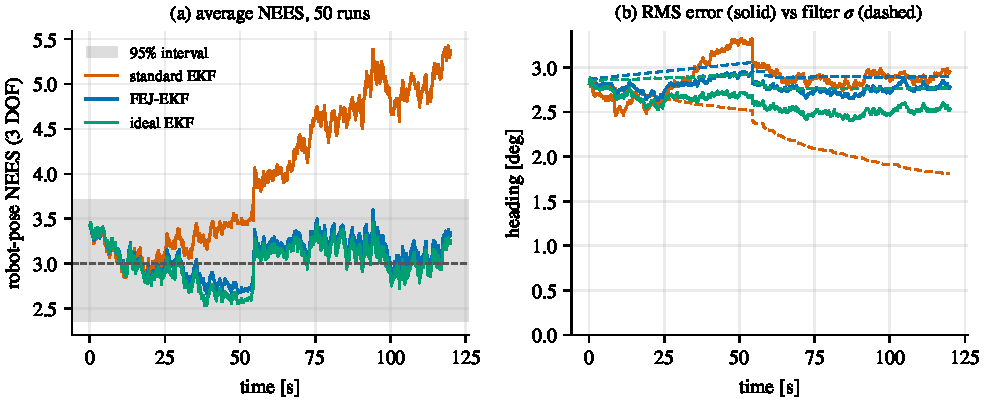
\includegraphics[width=\linewidth]{fig_fej.pdf}
\caption{Planar EKF-SLAM, 50 Monte Carlo runs. (a) Average NEES of the robot pose: the standard EKF leaves the 95\% interval after the first loop
closure (about \SI{55}{s}) and keeps rising, while the FEJ-EKF and the ideal EKF stay consistent. (b) Heading: actual RMS error (solid) and the
filter's own standard deviation (dashed). The initial heading is unobservable, so a consistent, realizable filter keeps reporting about its initial
\SI{2.9}{\degree}, as the FEJ-EKF does. The standard EKF's reported uncertainty falls to \SI{1.8}{\degree} while its actual error stays near \SI{3}{\degree}.}
\label{fig:fej}
\end{figure}

\subsection{A numerical demonstration}

\Cref{fig:fej} compares three filters on the same simulated data (\code{scripts/planar\_sims.py}). A robot drives almost twice around a circle of
radius \SI{10}{m} at \SI{1}{m/s} (\SI{120}{s}), sampling odometry at \SI{10}{Hz} (per-sample noise \SI{0.05}{m/s} in speed and \SI{0.01}{rad/s} in turn
rate), and measures the body-frame position of every landmark within \SI{5}{m} (20 landmarks are scattered around the circle), with \SI{0.1}{m} noise
per axis. The initial pose estimate has \SI{0.1}{m} position and
\SI{0.05}{rad} heading uncertainty. The three filters differ only in where they evaluate their Jacobians:
\begin{itemize}
  \item the \emph{standard EKF} uses the latest estimates, \eqref{eq:slam-phi}--\eqref{eq:slam-H};
  \item the \emph{FEJ-EKF} follows \cref{prop:fej};
  \item the \emph{ideal EKF} evaluates every Jacobian at the true state. It is not realizable, but it is the benchmark for consistency, since its
        linearized model has the true nullspace.
\end{itemize}
The heading panel makes the failure concrete. The initial heading error is unobservable, so no realizable filter can reduce it: the RMS heading
error of the standard and FEJ filters stays near its initial value of about \SI{2.9}{\degree}. (The ideal EKF reduces it slightly, to \SI{2.5}{\degree}, because
its Jacobians are evaluated at the true state, which leaks information that no real filter has.) The FEJ and ideal filters report standard
deviations that match their errors. The standard EKF reports a standard deviation that shrinks steadily, fastest at the loop closure, until its
variance is less than 40\% of its actual mean squared error. It has ``learned'' the global heading from relative measurements, which is impossible. Its NEES grows accordingly, and nothing in its
innovations reveals the problem.

\subsection{FEJ in the MSCKF}

The rule generalizes directly~\cite{li2013msckf2}: \emph{every state appears in the observability matrix at a single linearization point}. Concretely:
\begin{enumerate}
  \item \textbf{Propagation.} The transition matrix from $t_k$ to $t_{k+1}$ is evaluated with the propagated estimates at both ends,
        $\hat x_{k|k-1}$ and $\hat x_{k+1|k}$, wherever it depends on the state (positions, velocities, attitudes). The test is the planar one: the product of
        consecutive transition matrices must telescope.
  \item \textbf{Measurement.} Each clone enters the camera Jacobians at its \emph{first estimate}, the pose it had when it was cloned, not its
        current corrected value. The residual still uses the current value.
  \item \textbf{Feature.} The feature position used in $H_{x,j}$ and $H_{f,j}$ can be any single estimate (for example the triangulation from the
        current clone estimates), because the feature is eliminated: $A_j\T H_{f,j}N_f = 0$ for whatever $N_f$ the chosen value implies.
\end{enumerate}
The precise formulas depend on the error parameterization. For yours, the systematic procedure is: write $N$ in your error coordinates
(\eqref{eq:nullspace-N}), then choose the linearization points so that $\Phi_kN_k = N_{k+1}$ and $H_kN_k = 0$ hold \emph{exactly}, with $N_k$ built from the
first estimates. Even attitude blocks that do not seem to depend on the state may need attention: with a local attitude error, the yaw entry
$\hat R\T e_z$ of $N$ depends on the attitude estimate, so the attitude block of $\Phi_k$ must map $\hat R_{k|k-1}\T e_z$ to $\hat R_{k+1|k}\T e_z$.

\begin{implnote}[storing first estimates without allocation]
FEJ needs, for each clone, a second copy of its pose (the first estimate) next to the current one, and for the IMU state the propagated
estimate of the previous step. Both fit in fixed-size arrays sized by \code{kMaxClones}, so the zero-allocation rules of AGENTS.md E4 are
unaffected. A direct test: on a synthetic run, compute $\|\mathcal{O}N\|$ (or simply $\|H_kN_k\|$ and $\|\Phi_kN_k - N_{k+1}\|$ at every step) for the
standard and the FEJ filter. The FEJ values should be at rounding level, the standard ones visibly larger.
\end{implnote}

% ------------------------------------------------------------------------------
\section{Other remedies}

\subsection{Observability-constrained EKF}
\index{observability-constrained EKF}

Instead of choosing linearization points, the observability-constrained EKF (OC-EKF)~\cite{hesch2014consistency} computes Jacobians at
the latest estimates and then modifies them minimally so that the nullspace conditions hold.

\begin{proposition}[Minimal Jacobian corrections]
\label{prop:oc-ekf}
Let $N_k$ have full column rank. The matrix closest to $H$ in the Frobenius norm that satisfies $H^*N_k = 0$ is
\begin{equation}
  H^* = H\big(I - N_k(N_k\T N_k)\inv N_k\T\big),
\end{equation}
and the matrix closest to $\Phi$ that satisfies $\Phi^*N_k = N_{k+1}$ is
\begin{equation}
  \Phi^* = \Phi + (N_{k+1} - \Phi N_k)(N_k\T N_k)\inv N_k\T .
\end{equation}
\end{proposition}
\begin{proof}
The Frobenius norm is the sum of the squared norms of the rows, and the constraints act on each row separately: row $h$ must satisfy
$h^*N_k = c$ for a given row vector $c$ ($c = 0$ for $H$, a row of $N_{k+1}$ for $\Phi$). Minimizing $\|h^* - h\|^2$ subject to $h^*N_k = c$ is a least-norm problem
for the correction $d = h^* - h$: $dN_k = c - hN_k$. Its minimum-norm solution is $d = (c - hN_k)(N_k\T N_k)\inv N_k\T$ (\cref{sec:least-squares}), which gives both
formulas.
\end{proof}

The OC-EKF thus projects the information along $N$ out of every measurement and enforces the correct propagation of $N$, so the linearized
model has the correct unobservable subspace by construction. The choice of $N_k$ (which estimates to build it from) still matters; Hesch et
al.\ build it from the propagated estimates.

\subsection{Invariant EKF}
\index{invariant EKF}\index{extended pose group}

The invariant EKF~\cite{barrau2017invariant} attacks the root cause: the estimate dependence of $N$. It represents the IMU state as one element
of the \emph{extended pose group} $\mathrm{SE}_2(3)$,
\begin{equation}
  X = \begin{bmatrix} R & v & p \\ 0 & 1 & 0 \\ 0 & 0 & 1 \end{bmatrix} \in \R^{5\times5}, \qquad
  X\inv = \begin{bmatrix} R\T & -R\T v & -R\T p \\ 0 & 1 & 0 \\ 0 & 0 & 1 \end{bmatrix},
\end{equation}
a generalization of $\SE$ (\cref{sec:se3}) with two translation-like columns (features can be appended as further columns), and it defines the
error as the \emph{right-invariant} group error $\eta = \hat XX\inv = \Exp(\xi)$, with $\xi = (\xi_R, \xi_v, \xi_p) \in \R^9$.

\begin{proposition}[Constant unobservable directions]
\label{prop:invariant-nullspace}
In right-invariant error coordinates, the four unobservable directions of \cref{thm:vio-unobservable} are the constant vectors
$\xi = (e_z, 0, 0)$ (yaw) and $\xi = (0, 0, t)$, $t \in \R^3$ (translation), independent of the estimate.
\end{proposition}
\begin{proof}
A global yaw and translation act on the true state from the left: $X \mapsto GX$ with $G = \begin{bmatrix} R_z & 0 & t \\ 0 & 1 & 0 \\ 0 & 0 & 1\end{bmatrix}$, which is
$p \mapsto R_zp + t$, $v \mapsto R_zv$, $R \mapsto R_zR$. The error becomes $\hat X(GX)\inv = \hat XX\inv G\inv = \eta\,G\inv$. For small errors and a small
$G = \Exp(\epsilon)$, with $\epsilon = (\alpha e_z, 0, t)$, the product $\Exp(\xi)\Exp(-\epsilon)$ is $\Exp(\xi - \epsilon)$ to first order. The family of
indistinguishable states therefore differs, in error coordinates, by the constant vectors $\epsilon$.
\end{proof}

Compare \eqref{eq:nullspace-N}, where the yaw direction involves $\hat p$, $\hat v$ and $\hat R$. Because the group structure couples rotation with velocity
and position, a global yaw is a pure rotation error in these coordinates. Two consequences follow. The linearized error dynamics of the IMU (without
biases) are independent of the estimate, $\dot\xi = A\xi + \dots$ with
$A = \begin{bmatrix} 0 & 0 & 0 \\ \sx{g_w} & 0 & 0 \\ 0 & I & 0 \end{bmatrix}$, and $AN = 0$ because $\sx{g_w}e_z = 0$; and since every measurement is invariant under
$X \mapsto GX$, every measurement Jacobian, evaluated at \emph{any} estimate, annihilates the constant $N$. The linearized filter has the correct
unobservable subspace by construction, with no bookkeeping of first estimates. Biases break the exact estimate-independence of the error dynamics,
but not this nullspace property, since $N$ has no bias components. The price is a different state representation, different Jacobians, and a different reset;
it is a deviation from AGENTS.md C3--C4 that this project does not take.

\subsection{Robocentric formulations}
\index{robocentric filter}

A robocentric filter expresses everything relative to the current body frame, so the unobservable global quantities are not estimated at all,
and the global pose is recovered by composing relative motions outside the filter. The nullspace problem disappears with the unobservable states,
at the cost of a more complex propagation in which every state moves when the body moves.

\begin{center}\small
\begin{tabularx}{\linewidth}{@{}l>{\raggedright\arraybackslash}X>{\raggedright\arraybackslash}X@{}}
\toprule
Remedy & What changes & Cost \\
\midrule
FEJ & linearization points of $\Phi$ and $H$ & store first estimates; slightly larger linearization error \\
OC-EKF & Jacobians projected onto the constraint & build $N_k$ each step; extra products \\
Invariant EKF & state representation and error definition & new derivations; leaves the frozen conventions \\
Robocentric & state is relative to the body & more complex propagation \\
\bottomrule
\end{tabularx}
\end{center}

% ------------------------------------------------------------------------------
\section{Degenerate motions}
\index{degenerate motions}

\Cref{thm:vio-unobservable} assumes \emph{general} motion. Some motions remove further directions~\cite{yang2019degenerate}.
\begin{center}\small
\begin{tabular}{@{}l l@{}}
\toprule
Motion & What becomes unobservable \\
\midrule
constant velocity (no acceleration) & metric scale \\
pure rotation (no translation) & feature depths and translation scale \\
no rotation & accelerometer bias inseparable from the gravity direction (tilt) \\
at rest & both of the above, plus everything that needs parallax \\
\bottomrule
\end{tabular}
\end{center}
Each row has a short explanation. At constant velocity the accelerometer measures only gravity and bias, so nothing ties the size of the
camera's (scale-free) motion estimate to meters. Without translation there is no parallax, so depths, and with them the scale of the
translation, cannot be triangulated. Without rotation the gravity direction in the body frame is constant, and a constant error in it is
indistinguishable from a constant accelerometer bias; rotation makes gravity sweep through the body axes while the bias stays fixed, which
separates them.

The filter does not fail during such motions, provided it is consistent: its covariance simply stops shrinking along the
affected directions until informative motion returns. An inconsistent filter, by contrast, may ``learn'' these quantities from
noise. When a vehicle is known to be stationary, a \emph{zero-velocity update} (the pseudo-measurement $v = 0$, \cref{ch:updates}) supplies real
information and stops drift, which is why many systems detect stillness explicitly.

\begin{takeaways}
\begin{itemize}
  \item The unobservable subspace is the nullspace of the observability matrix; a filter must not gain information along it. For nonlinear
        systems, the gradients of the output's Lie derivatives play the role of the observability matrix.
  \item VIO has four unobservable directions: global translation and rotation about gravity. Roll, pitch and scale are observable
        under general motion.
  \item In local error coordinates the yaw direction is $\hat R\T e_z$ for the attitude and $-\sx{\hat p}e_z$ for positions: it depends on
        the estimate.
  \item Linearizing the same state at different estimates makes the global heading spuriously observable: in planar SLAM the leak is
        $\hat R_k\T\Omega(D_k + \bar\ell_j - \hat\ell_j)$, driven by the accumulated corrections and the drift of the landmark estimates.
  \item FEJ restores the nullspace by fixing each state's linearization point; OC-EKF projects the Jacobians; the invariant EKF makes the
        unobservable directions constant; degenerate motions remove further directions.
\end{itemize}
\end{takeaways}

\begin{exercises}
  \item Verify \eqref{eq:nullspace-N} numerically: apply a small yaw rotation and translation to a random state and compute
        $x'\bminus x$.
  \item Show that the translation columns of $N$ remain in the nullspace of the EKF's observability matrix even when Jacobians are
        evaluated at changing estimates.
  \item Redo the worked example on Lie derivatives with two unknown landmarks. What is the rank of $d\mathcal{O}$, and what are the unobservable
        directions?
  \item Repeat \cref{thm:slam-obs} for range-and-bearing measurements, $z = (\|d\|, \atantwo(d_y, d_x))$ with $d = R(\psi)\T(\ell_j - p)$. Show that the leak
        has the same form.
  \item Modify \code{scripts/planar\_sims.py} to print $\|H_k\Phi_{k-1}\cdots\Phi_1N\|$ for the three filters of \cref{fig:fej}, and confirm that only the
        standard EKF violates the nullspace condition.
  \item Prove that the minimum-norm solution used in \cref{prop:oc-ekf} is indeed the minimizer, by writing $d = d_\parallel + d_\perp$ with $d_\parallel$ in the row space of
        $N_k\T$.
  \item Implement a zero-velocity update as an EKF measurement and derive its $H$. When is it safe to apply?
  \item Read~\cite{li2013msckf2} and list which Jacobians must be evaluated at first estimates in the MSCKF. Sketch how you would store
        the first estimates in the project's data structures without allocation.
\end{exercises}

\chapter{Engineering a Real-Time Estimator in C++20}
\label{ch:engineering}
\chaptermark{Engineering in C++20} % short running header
\sloppy % long code identifiers cannot be hyphenated

\begin{objectives}
\begin{itemize}
  \item Know the C++ facts an estimator depends on: stack and heap, object lifetime, and the C++20 features the project uses.
  \item Understand why a real-time estimator must be deterministic, and how the project's memory tiers achieve it.
  \item Know how Eigen represents matrices, blocks and expressions, and use fixed-max-size matrices, member workspaces and
        allocation guards correctly.
  \item Avoid the Eigen pitfalls that silently corrupt numbers: dangling expression templates and aliasing.
  \item Understand what the sanitizers check and how, and how a target-based CMake build is organized.
  \item Design a test strategy in which every test can fail, and a systematic procedure for debugging a diverging filter.
\end{itemize}
\end{objectives}

The mathematics of the previous chapters is necessary but not sufficient. An estimator that is mathematically correct can still
miss its deadline because of an allocation, produce garbage because of an Eigen expression template, or pass all its tests because
the tests cannot fail. This chapter collects the engineering practices that the project encodes in AGENTS.md.

% ------------------------------------------------------------------------------
\section{C++ essentials for estimator code}
\label{sec:cpp-essentials}

\subsection{Stack, heap and object lifetime}

A C++ program keeps its data in two kinds of memory. The \term{stack} holds the local variables of the functions currently running. Entering a
function reserves a block of it by moving a pointer, and leaving the function releases the block by moving the pointer back: the cost is a
few instructions, it is the same every time, and the size of each block is fixed at compile time. The \term{heap} holds objects whose size or
lifetime is decided at run time. Obtaining heap memory (\code{new}, \code{std::vector} growth, a dynamic-size Eigen matrix) calls the memory
allocator, which must find a free block of the right size, may take a lock shared with other threads, and occasionally asks the operating
system for more pages. Its cost is usually modest and occasionally large, which is exactly what a real-time loop cannot afford.

Every C++ object has a lifetime that ends at a precisely defined point: a local variable when its scope closes, a member when its owner is
destroyed. At that point its destructor runs. Tying resources (memory, files, locks) to object lifetime is called \term{RAII} (resource
acquisition is initialization): a \code{std::vector} frees its heap block in its destructor, so it cannot leak. The project uses RAII
everywhere and never calls \code{delete} by hand. The stack is small (typically \SI{1}{MB} on Windows, \SI{8}{MB} on Linux), so large
matrices belong in class members created once, not in function locals.

\subsection{The C++20 features the project uses}

\begin{lstlisting}
inline constexpr int kImuDim = 15;   // compile-time constant, one definition

[[nodiscard]] bool update(const PoseMeasurement& z) noexcept; // result must be used
void ingest(std::span<const ImuSample> samples) noexcept;     // view of contiguous data
\end{lstlisting}

\begin{itemize}
  \item \code{constexpr} values are computed at compile time and can size arrays and Eigen matrices; \code{inline constexpr} in a header gives one
        shared definition. Dimensions, indices (AGENTS.md C3) and the $\chi^2$ table are \code{constexpr}.
  \item \code{[[nodiscard]]} makes the compiler warn (with \code{-Werror}, fail) when a caller ignores the return value: a rejected update or a failed
        factorization must not be silently dropped.
  \item \code{noexcept} promises that a function throws no exception. If one escapes anyway the program terminates, so the promise is only made
        on the hot path, where errors are reported through return values instead.
  \item \code{std::span<const T>} is a non-owning view (a pointer and a length) of contiguous elements. A function taking a span accepts an array, a
        \code{std::vector} or part of one without copying and without caring who owns the memory.
  \item \code{std::variant<A, B>} holds exactly one of several types, without heap allocation. \code{std::visit} calls the matching overload:
\end{itemize}

\begin{lstlisting}
template <class... Ts> struct Overloaded : Ts... { using Ts::operator()...; };
template <class... Ts> Overloaded(Ts...) -> Overloaded<Ts...>;

for (const SensorEvent& event : events) {           // one presorted stream
  std::visit(Overloaded{
      [&](const ImuSample& s)  { filter.propagate(s); },
      [&](const ImageEvent& e) { pipeline.on_image(e); },
  }, event);
}
\end{lstlisting}

\code{Overloaded} inherits the call operators of all the lambdas passed to it, so \code{std::visit} finds the one whose parameter type matches the
alternative currently stored. Adding a new event type to the variant without handling it is a compile error, not a silent omission.

% ------------------------------------------------------------------------------
\section{Determinism and the memory tiers}

A flight controller consumes the estimator's output at a fixed rate. A late estimate is a wrong estimate. The main source of
unpredictable latency in C++ is dynamic memory allocation: \code{new}, a \code{std::vector} that grows, a dynamic-size Eigen temporary. The
allocator may take locks, search free lists or ask the operating system for pages, with latency that is usually small and
occasionally large. The project therefore separates three tiers (AGENTS.md E4).

\begin{center}\small
\begin{tabularx}{\textwidth}{@{}l X X@{}}
\toprule
Tier & Scope & Rule \\
\midrule
Load & parsing, building event arrays, constructing the filter & allocate freely, before streaming starts \\
Core & \code{vio\_core}, per IMU sample and per update & zero heap allocations \\
Frontend & OpenCV tracking & may allocate, must reuse buffers; allocations are measured and logged \\
\bottomrule
\end{tabularx}
\end{center}

\subsection{Fixed-max-size matrices}

The MSCKF covariance changes size as clones come and go, but never exceeds $15 + 6N_{max}$. Eigen supports exactly this case: a
matrix whose \emph{runtime} size is dynamic but whose \emph{maximum} size is a compile-time constant. Its storage is an inline array of the
maximum size, so resizing within the bound never allocates.

\begin{lstlisting}
inline constexpr int kMaxClones = 10;                  // decided in M10a
inline constexpr int kMaxDim    = 15 + 6 * kMaxClones;

using CovMatrix = Eigen::Matrix<double, Eigen::Dynamic, Eigen::Dynamic,
                                Eigen::ColMajor, kMaxDim, kMaxDim>;

CovMatrix P;          // inline storage for 75 x 75 doubles, no heap
P.resize(15, 15);     // allowed: within the compile-time maximum
\end{lstlisting}

Large workspaces ($S$, $K$, stacked $H$, temporaries for $\Phi P$) are class members, created once, rather than function-local
variables. Function-local fixed-max matrices would not allocate either, but they would live on the stack, and several of them at
once can exceed it (\cref{ch:cloning}).

\subsection{Proving it: allocation guards}

``It shouldn't allocate'' is not evidence. The project overrides the global \code{operator new} in its tests to count allocations
(\code{tests/support/alloc\_guard.hpp}), and wraps every core hot-path test with a guard that asserts a count of zero. In debug builds,
\code{EIGEN\_RUNTIME\_NO\_MALLOC} together with \code{Eigen::internal::set\_is\_malloc\_allowed(false)} makes Eigen itself abort on any internal
allocation and reports where it happened. Both mechanisms are needed, because they see different allocations. The guard sees everything that goes
through \code{operator new}: \code{std::vector} growth, \code{std::string}, \code{std::function}, \code{std::make\_unique}. Eigen, however, obtains its heap memory
directly from \code{std::malloc} through its own aligned allocator, so a dynamic \code{Eigen::MatrixXd} is invisible to the guard. Only Eigen's flag catches it,
and only in the \code{debug-sanitize} preset, where the flag is defined.

% ------------------------------------------------------------------------------
\section{Eigen in brief}
\label{sec:eigen-basics}
\index{Eigen}\index{expression templates}

\paragraph{The matrix type.} Every dense Eigen matrix is an instance of one class template,
\begin{lstlisting}
Eigen::Matrix<Scalar, Rows, Cols, Options, MaxRows, MaxCols>
\end{lstlisting}
\code{Rows} and \code{Cols} are either compile-time numbers (a \emph{fixed-size} matrix such as \code{Eigen::Matrix3d}, stored inline with no heap) or
\code{Eigen::Dynamic} (size chosen at run time, normally on the heap, such as \code{Eigen::MatrixXd}). \code{MaxRows} and \code{MaxCols} give a dynamic
matrix a compile-time upper bound, which turns its storage into an inline array: the fixed-max-size matrices used below. \code{Options} chooses the
storage order.

\paragraph{Storage order.} Memory is one-dimensional. A \emph{column-major} matrix (Eigen's default) stores column after column, so entry $(i, j)$ of
an $m\times n$ matrix lives at offset $i + jm$; a \emph{row-major} matrix stores row after row, offset $j + in$. Loops are fastest when they walk
memory contiguously, so with column-major storage the inner loop should run down a column. Mixing orders is legal but may force copies.

\paragraph{Blocks.} \code{P.block(i, j, r, c)}, \code{P.topLeftCorner(15, 15)}, \code{v.segment<3>(6)} and their relatives return \emph{views}: they refer to
the original storage, copy nothing, and can be assigned to. \code{P.block<3, 3>(6, 6) = ...} writes the attitude block of $P$ in place. The fixed-size
forms (template arguments) let Eigen unroll small operations completely.

\paragraph{Passing matrices and blocks to functions.} A parameter of type \code{const Eigen::Matrix3d\&} accepts only that exact type. To accept any
matrix or block of compatible layout, use \code{Eigen::Ref<const Eigen::MatrixXd>} (read-only) or \code{Eigen::Ref<Eigen::MatrixXd>} (writable). A
read-only \code{Ref} quietly makes a temporary copy when the argument's layout is incompatible, and for a dynamic type that copy allocates; a writable
\code{Ref} refuses to compile instead. The quiet copy is an Eigen allocation, so \code{EIGEN\_RUNTIME\_NO\_MALLOC} catches it and the
\code{operator new} guard does not.

\paragraph{Wrapping existing memory.} \code{Eigen::Map<const Eigen::Vector3d> v(ptr)} views three doubles at \code{ptr} as a vector, without copying.
It is the right tool for parsed buffers, and the wrong one for quaternions read from EuRoC: \code{Eigen::Map<Eigen::Quaterniond>} interprets memory as
$(x, y, z, w)$, while the CSV stores $(w, x, y, z)$ (AGENTS.md C2).

\paragraph{Expression templates.} \code{A + B} does not compute a matrix. It returns a small object recording ``the sum of \code{A} and \code{B}''. Only when
that object is assigned to a matrix does Eigen run a loop, and it fuses the whole expression into it: \code{D = A + B + C} is one loop with no
temporaries. Products are the exception: they are evaluated into a temporary unless told otherwise (below). This design makes Eigen fast, and it
is also the source of the \code{auto} pitfall described next.

\paragraph{Decompositions.} Linear systems are solved through decomposition objects: \code{S.llt().solve(B)} (Cholesky, for symmetric positive definite
$S$), \code{.ldlt()} (robust for semi-definite), \code{.householderQr()} and \code{.colPivHouseholderQr()} (QR, \cref{ch:numlinalg}). A decomposition object owns
a copy of the factor; for fixed-max matrices that copy is inline. \code{Eigen::LLT<Eigen::Ref<Eigen::MatrixXd>{}> llt(A)} factors \code{A} \emph{in place},
overwriting it with the factor and allocating nothing. Symmetric structure can be exploited with \code{P.selfadjointView<Eigen::Lower>()}, which reads
only one triangle.

% ------------------------------------------------------------------------------
\section{Eigen pitfalls}

\paragraph{Expression templates and \code{auto}.} Eigen operations return lightweight \emph{expression} objects that are evaluated
lazily, when they are assigned to a matrix. An expression holds the matrices it uses by reference and nested expressions by value. Storing one
with \code{auto} therefore has two dangers. If a referenced matrix is a temporary (made by \code{.eval()}, or returned by value from a function),
the reference dangles. And even if every operand still exists, the computation happens only at the later assignment, with whatever values
the operands have then.

\begin{lstlisting}
auto bad = (a + b).eval().transpose(); // refers to the temporary made by eval()
Eigen::RowVector3d x = bad;            // undefined behavior: that temporary is gone
Eigen::RowVector3d good = (a + b).transpose(); // concrete type: evaluated now

auto lazy = A * v;                     // nothing is computed here
A(0, 0) = 10.0;
Eigen::Vector3d y = lazy;              // computed now, with the modified A
\end{lstlisting}

The rule is simple: never use \code{auto} with Eigen expressions (AGENTS.md E5). Name the concrete type, or call \code{.eval()} when a
temporary really is wanted. AddressSanitizer reports the dangling case (as a use after scope), but not the stale one, which reads only valid
memory (Exercise~30.2).

\paragraph{Aliasing.} Eigen assumes that the destination of a matrix product may alias its operands and evaluates products into a
temporary. With dynamic sizes that temporary allocates. When the destination is known not to alias, \code{.noalias()} writes directly
into it. When it does alias, the temporary is required: write into a member workspace explicitly.

\begin{lstlisting}
tmp_15xN_.noalias() = Phi * P.topRightCorner(15, nc);  // reads P, writes workspace
P.topRightCorner(15, nc) = tmp_15xN_;                   // copy back
P.bottomLeftCorner(nc, 15) = tmp_15xN_.transpose();     // keep symmetry
\end{lstlisting}

Coefficient-wise operations do not alias-check. \code{A = A.transpose()} is the classic bug; use \code{A.transposeInPlace()} or symmetrize
with a workspace.

\paragraph{Passing and alignment.} Pass Eigen objects by \code{const\&} (or \code{Eigen::Ref} for blocks). Do not add
\code{EIGEN\_MAKE\_ALIGNED\_OPERATOR\_NEW}: since C++17, aligned \code{new} handles over-aligned types. The real alignment hazard is mixing
\code{-march} or alignment-changing flags between translation units or with dependencies, which the project forbids.

\paragraph{Decompositions without allocation.} Eigen's decompositions normally own their storage. Fixed-max decomposition objects held as
members, or the in-place variants that factor a matrix in its own storage, avoid per-call allocation. Whatever the API, verify with
\code{EIGEN\_RUNTIME\_NO\_MALLOC}, which sees Eigen's allocations where the \code{operator new} guard cannot.

% ------------------------------------------------------------------------------
\section{Time and events}

\begin{lstlisting}
using Clock = std::chrono::nanoseconds;
struct ImuSample   { Clock t; Eigen::Vector3d gyro, accel; };
struct ImageEvent  { Clock t; int index; };
using SensorEvent = std::variant<ImuSample, ImageEvent /*, PoseMeasurement */>;

// Delta t: subtract in integers, convert only the difference.
const double dt = std::chrono::duration<double>(t1 - t0).count();
\end{lstlisting}

Absolute time stays in 64-bit integer nanoseconds (\cref{sec:floating}). Events form one presorted sequence built at load time, so the
streaming loop is a single pass over contiguous memory, dispatched with \code{std::visit} as in \cref{sec:cpp-essentials}: no priority queue, no
allocation, no reordering surprises.

% ------------------------------------------------------------------------------
\section{Numerical robustness checklist}

\begin{itemize}
  \item Normalize every quaternion after every multiplicative update (propagation, injection, cloning).
  \item Symmetrize $P$ after propagation and after every update.
  \item Use the Joseph form; factor $S$ with Cholesky or LDL$^\mathsf{T}$; treat a failed factorization as an error to report, not to hide.
  \item Guard every $0/0$ with Taylor branches; use $\atantwo$ for angles; handle $\Log$ near $\pi$.
  \item Reject features with non-positive or tiny depth, poor parallax or large reprojection error before linearizing.
  \item Count and log gate rejections and triangulation failures.
  \item Never clamp negative eigenvalues of $P$ to hide a problem; find out why they appeared.
  \item In debug builds, assert finiteness at module boundaries so that a \code{NaN} is caught where it is born.
\end{itemize}

% ------------------------------------------------------------------------------
\section{Sanitizers}
\label{sec:sanitizers}
\index{sanitizers}\index{AddressSanitizer}\index{UndefinedBehaviorSanitizer}

C++ leaves many errors undefined: reading past the end of an array, using memory after freeing it, overflowing a signed integer. Undefined
behavior does not mean a crash; it means the compiler may assume it never happens, so the program can produce plausible wrong numbers, behave
differently between builds, or fail far from the bug. Sanitizers are compiler-inserted checks that turn these silent errors into immediate,
precise reports.
\begin{itemize}
  \item \textbf{AddressSanitizer} (ASan, \code{-fsanitize=address}) keeps a \emph{shadow memory}, one byte for every eight bytes of program memory,
        recording which bytes may be accessed. Every heap block, stack variable and global is surrounded by poisoned \emph{redzones}, and freed
        memory stays poisoned for a while. The compiler inserts a shadow check before every load and store. ASan reports heap, stack and
        global buffer overflows, use after free, use after scope and double frees, with stack traces of the access and of the allocation. The
        cost is roughly a factor of two in speed and three in memory.
  \item \textbf{UndefinedBehaviorSanitizer} (UBSan, \code{-fsanitize=undefined}) inserts checks for signed integer overflow, out-of-range shifts, integer
        division by zero, null and misaligned pointer use, invalid \code{bool} and \code{enum} values, and floating-point-to-integer conversions that
        overflow.
\end{itemize}
By default UBSan prints a message and \emph{continues}, so a test that triggers it still passes. \code{-fno-sanitize-recover=all} makes every report
abort the process, and the test preset sets \code{UBSAN\_OPTIONS=print\_stacktrace=1:halt\_on\_error=1} so the report carries a stack trace
(AGENTS.md E3). Frame pointers (\code{-fno-omit-frame-pointer}) make those traces reliable. On Windows, LeakSanitizer does not exist, so leaks are
not detected (RAII makes them rare), and an instrumented executable needs the ASan runtime DLL from \code{C:\textbackslash msys64\textbackslash clang64\textbackslash bin}
on its \code{PATH}. Sanitizers are a debug-build tool: the \code{release} preset builds without them, and both presets must pass.

% ------------------------------------------------------------------------------
\section{Modern CMake in brief}
\label{sec:cmake}
\index{CMake}

CMake describes a build as a set of \emph{targets} (libraries and executables) with properties. Modern CMake attaches every setting to a target
rather than to global variables, and lets settings propagate along the dependency graph through three keywords:
\code{PRIVATE} (used to build this target only), \code{INTERFACE} (used only by targets that link to this one) and \code{PUBLIC} (both). A library's public
include directory is \code{PUBLIC}, because its users include its headers; a warning flag is \code{PRIVATE}, because it concerns only the library's
own code.

\begin{lstlisting}
add_library(vio_warnings INTERFACE)            # carries flags, builds nothing
target_compile_options(vio_warnings INTERFACE -Wall -Wextra -Wconversion -Werror)

add_library(vio_core STATIC src/so3.cpp src/es_ekf.cpp)
target_include_directories(vio_core PUBLIC include)
target_link_libraries(vio_core PUBLIC Eigen3::Eigen PRIVATE vio_warnings)
\end{lstlisting}

The \code{vio\_warnings} target is how warnings stay off the dependencies (AGENTS.md E3): only project targets link it. Dependencies fetched with
\code{FetchContent} at a pinned tag are declared \code{SYSTEM}, so their headers are included with \code{-isystem} and do not trigger the project's warnings.
\code{CMakePresets.json} stores named configurations (generator, compiler, build type, flags, test environment), so that
\code{cmake --preset debug-sanitize}, \code{cmake --build --preset debug-sanitize} and \code{ctest --preset debug-sanitize} reproduce exactly the same build
on every machine. Catch2's \code{catch\_discover\_tests} registers each \code{TEST\_CASE} as a separate CTest test.

% ------------------------------------------------------------------------------
\section{Testing}

\begin{keyidea}[a test must be able to fail]
For every test, ask: would it still pass if I flipped the sign of X, transposed Y, or swapped two blocks? If yes, the test is
decoration. Run it once against a deliberately broken implementation to make sure it fails.
\end{keyidea}

The project's test strategy layers several kinds of evidence.
\begin{enumerate}
  \item \textbf{Algebraic unit tests}: identities such as $\Log(\Exp(\phi)) = \phi$ at zero, tiny, generic and near-$\pi$ angles.
  \item \textbf{Finite-difference Jacobian tests} built on $\bplus/\bminus$, at non-trivial states, with tolerances justified in a comment.
  \item \textbf{Closed-form trajectory tests}: synthetic trajectories with analytic IMU data and convergence-order checks.
  \item \textbf{Statistical tests}: Monte Carlo covariance checks and NEES/NIS with $\chi^2$ bounds, seeded with
        \code{std::mt19937\_64}. Because \code{std::normal\_distribution} differs between standard libraries, never hard-code values from one
        run; test statistical properties.
  \item \textbf{Invariance tests}: cloning enabled versus disabled must give identical IMU estimates when no visual updates occur.
  \item \textbf{Resource tests}: allocation guards around every core hot path.
  \item \textbf{Sanitizers}: ASan and UBSan builds with \code{-fno-sanitize-recover=all}, so that any report fails the test run
        (\cref{sec:sanitizers}).
\end{enumerate}

% ------------------------------------------------------------------------------
\section{Debugging a diverging filter}

When the full system misbehaves, resist the urge to tune. Work down the layers instead.
\begin{enumerate}
  \item Run on \textbf{synthetic data} with exactly modeled noise. If it fails there, the bug is in the code.
  \item Disable visual updates. Does IMU-only propagation from ground truth behave as \cref{fig:cov-growth} predicts, with errors
        inside $3\sigma$?
  \item Replace visual updates by \textbf{pose updates} (Milestone 6). If those are consistent, the back end is sound.
  \item Feed the MSCKF \textbf{ground-truth feature tracks} from a synthetic scene. If that works, the problem is in the front end or the
        calibration.
  \item On real data, plot each residual component over time and look for bias, oscillation or outliers.
  \item Only then adjust noise parameters, and judge the result on consistency statistics.
\end{enumerate}

\section{Going further}

Once the baseline MSCKF runs, natural extensions are First-Estimates Jacobians (\cref{ch:observability}); online calibration of the
camera-IMU extrinsics and time offset~\cite{li2013msckf2, li2014timeoffset}; stereo observations from \code{cam1}; keeping long-lived
features as SLAM landmarks; zero-velocity updates; and evaluation on the harder EuRoC sequences (V1\_03, MH\_05) and other
datasets. Each extension adds states and Jacobians, and each Jacobian gets its derivation and its finite-difference test.

\begin{takeaways}
\begin{itemize}
  \item Heap allocation has unpredictable cost; the stack is cheap but small. Large workspaces are members, created once.
  \item Determinism requires zero allocation in the core: fixed-max-size matrices, member workspaces, proven by allocation guards and
        \code{EIGEN\_RUNTIME\_NO\_MALLOC} (Eigen allocates with \code{malloc}, which the guard does not see).
  \item Never use \code{auto} with Eigen expressions; use \code{.noalias()} only when there is no aliasing.
  \item Keep time in integer nanoseconds and process one presorted event stream.
  \item Sanitizers turn undefined behavior into reports; without \code{-fno-sanitize-recover=all} UBSan reports do not fail tests.
  \item Every test must be able to fail; layer algebraic, Jacobian, closed-form, statistical and resource tests.
  \item Debug by removing layers until the failure disappears, not by tuning.
\end{itemize}
\end{takeaways}

\begin{exercises}
  \item Write a minimal allocation guard by overriding the global \code{operator new} and \code{operator delete}, and show that it detects a
        \code{std::vector::push\_back} beyond capacity but not a fixed-max Eigen \code{resize}.
  \item Construct an example in which \code{auto} with an Eigen expression produces wrong numbers without crashing. Does
        AddressSanitizer report it?
  \item Measure the time of 10\,000 covariance propagation steps with fixed-max and with fully dynamic Eigen matrices, in both build
        presets. Explain the difference.
  \item Take one of your Jacobian tests, break the Jacobian in three different ways, and record which breakages the test detects.
  \item Write a function that reads one element past the end of a \code{std::array} and another that overflows an \code{int}. Build both presets and
        record what each sanitizer reports, and what the release build does.
  \item Pass a row-major block to a function taking \code{Eigen::Ref<const Eigen::MatrixXd>} inside an allocation guard. What happens, and what
        happens if the parameter is a writable \code{Ref}?
  \item Add a third alternative to the \code{SensorEvent} variant without handling it in the \code{Overloaded} visitor. Read the compiler error.
\end{exercises}
% Solutions to the exercises of Chapter 30.
\begin{solutions}
  \item The core of a minimal guard:
\begin{lstlisting}
inline int g_allocations = 0;                  // reset before, check after
void* operator new(std::size_t n) {
  ++g_allocations;
  if (void* p = std::malloc(n)) return p;
  throw std::bad_alloc();
}
void operator delete(void* p) noexcept { std::free(p); }
void operator delete(void* p, std::size_t) noexcept { std::free(p); }
\end{lstlisting}
        Reset the counter immediately before the code under test and read it immediately after, because the test framework allocates too. Measured
        with clang/libc++:
        \begin{itemize}
          \item four \code{push\_back} calls into a vector with \code{reserve(4)}: 0 allocations; the fifth: 1 (the reallocation);
          \item resizing a fixed-max $75\times75$ matrix from $15\times15$ to $75\times75$: 0, because the storage is inline;
          \item a dynamic \code{Eigen::MatrixXd(10, 10)}: also 0. This is not because it does not allocate, but because Eigen allocates with \code{std::malloc}
                through its own aligned allocator, which never calls \code{operator new}.
        \end{itemize}
        With \code{EIGEN\_RUNTIME\_NO\_MALLOC} and \code{set\_is\_malloc\_allowed(false)}, the same \code{MatrixXd} aborts with Eigen's assertion ``heap allocation is forbidden''. The guard and
        the flag are therefore both needed. Since the flag is defined only in the \code{debug-sanitize} preset, Eigen allocations are caught only there. Defining it for the
        test targets of both presets would close that gap; it is a design decision to record in \code{PROGRESS.md}. A complete guard also overrides the aligned
        forms \code{operator new(std::size\_t, std::align\_val\_t)}, which the library implements without calling the plain one. The C++ experiments of these
        solutions are in \code{scripts/solutions/cpp}, with \code{build\_and\_run.ps1} to build and run them in both configurations.

  \item Five candidates, each assigned afterwards to a concrete type and built in both presets:
        \begin{itemize}
          \item \code{auto e = R * (a + b);} gives correct numbers in both builds. The sum is a nested expression, which Eigen stores by value, so nothing dangles.
          \item \code{auto e = (a + b).eval().transpose();} prints the right numbers in release, by luck. ASan reports \code{stack-use-after-scope}.
          \item \code{auto e = make().head<2>();}, with \code{make()} returning a \code{Vector3d} by value, behaves the same way: right by luck in release, reported by ASan.
          \item \code{auto e = (X * 2.0).eval().block(0, 0, 2, 2);} with a dynamic \code{X} prints garbage ($10^{-311}$ entries) in release without crashing.
                ASan reports \code{stack-use-after-scope}.
          \item \code{auto e = A * v;} followed by a change to \code{A} produces the product with the \emph{new} \code{A} in both builds, and no sanitizer reports anything.
        \end{itemize}
        Dangling references are undefined behavior: the optimized build may print the right numbers because
        the dead temporary's stack slot has not been reused yet, or garbage, as in the dynamic case. AddressSanitizer reports them reliably, as a read of a variable
        whose scope has ended. The stale expression is not undefined behavior at all, since every access is to valid memory. The expression is simply evaluated
        later than the reader assumed, so no sanitizer can report it. Only the rule ``no \code{auto} with Eigen'' prevents it.

  \item Ten thousand propagation steps of a $75\times75$ covariance (the $15\times15$ block with $\Phi P\Phi\T + Q$, the $15\times60$ cross block with $\Phi P_{IC}$), per step:
        \begin{center}\small
        \begin{tabular}{@{}l c c@{}}
        \toprule
        implementation & release & debug-sanitize \\
        \midrule
        fixed-max, member workspaces & \SI{3.0}{\micro\second} & \SI{500}{\micro\second} \\
        dynamic, temporaries in expressions & \SI{3.3}{\micro\second} & \SI{525}{\micro\second} \\
        dynamic, preallocated workspaces & \SI{3.3}{\micro\second} & \SI{505}{\micro\second} \\
        \bottomrule
        \end{tabular}
        \end{center}
        In release, the arithmetic (about $4\times10^4$ flops) dominates. The three small heap allocations per step of the naive dynamic version cost a few hundred
        nanoseconds, and fixed sizes let Eigen unroll the $15\times15$ parts. That gives a 10\% difference, not an order of magnitude. The dynamic version with workspaces does not allocate
        either (it ran with Eigen allocations forbidden). The case for fixed-max matrices is therefore not average speed but the \emph{guarantee}: the storage is
        inline, its bound is checked, and no forgotten \code{.noalias()} or temporary can allocate in the hot path. That is what makes the worst case predictable. The
        sanitizer build is about 170 times slower. At \code{-O0} none of Eigen's small template functions is inlined, and ASan checks every load and store. Use it to
        prove correctness (both allocation-free versions ran with \code{malloc} forbidden), never to measure speed.

  \item With the right Jacobian $\Jr$ of \cref{ch:lie}, tested against central differences of $\Log(\Exp(\phi)\T\Exp(\phi + \delta))$ ($h = 10^{-6}$, so the correct version agrees to $10^{-10}$), the
        largest error of three broken versions at four test points is:
        \begin{center}\small
        \begin{tabular}{@{}l c c c c@{}}
        \toprule
        breakage & $\phi = 0$ & $\|\phi\| = 0.05$ & $\|\phi\| = 0.5$ & $\|\phi\| = 2.5$ \\
        \midrule
        sign of the $\sx{\phi}$ term flipped (this is $\Jl$) & 0 & $4\times10^{-2}$ & $0.4$ & $1.1$ \\
        second-order term dropped & 0 & $4\times10^{-4}$ & $4\times10^{-2}$ & $0.65$ \\
        Taylor branch used below $0.1$~rad & 0 & $4\times10^{-4}$ & $8\times10^{-11}$ & $9\times10^{-11}$ \\
        \bottomrule
        \end{tabular}
        \end{center}
        A test at $\phi = 0$ detects nothing, since every version equals $I$ there. A test at a single generic angle misses the wrong branch threshold. A loose tolerance
        ($10^{-3}$, say) misses the dropped term at small angles. Hence the rules: several random points spanning the regimes (tiny, inside every branch, generic, near
        $\pi$), and a tolerance derived from the finite-difference error rather than chosen for comfort.

  \item Reading \code{a[4]} of a \code{std::array<int, 4>} and computing \code{INT\_MAX + 1}:
        \begin{itemize}
          \item \emph{release}: the read returned 1634890337 (whatever lay next on the stack) and the addition printed $-2147483648$. No crash and no message.
                Neither result is guaranteed: both are undefined behavior, and the optimizer may, for example, fold \code{x + 1 > x} to \code{true};
          \item \emph{debug-sanitize}: ASan stops at the read with \code{stack-buffer-overflow ... READ of size 4} and the file and line of the access. UBSan stops at the
                addition with \code{runtime error: signed integer overflow: 2147483647 + 1 cannot be represented in type 'int'}. With \code{-fno-sanitize-recover=all}
                both abort, so a test that triggers them fails.
        \end{itemize}
        Note that \code{std::array::operator[]} does not check bounds. ASan caught the read because the array lives on the stack between redzones. Compiling with libc++'s
        hardening (\code{-D\_LIBCPP\_HARDENING\_MODE=\_LIBCPP\_HARDENING\_MODE\_FAST}) adds a cheap bounds check that traps even in an optimized build: the process stopped with an
        illegal-instruction exception.

  \item Binding a $3\times3$ block of a row-major matrix to \code{Eigen::Ref<const Eigen::MatrixXd>} compiles and gives the right result, but \code{Ref} cannot describe a row-major block
        with column-major strides, so it copies the block into an internal \code{MatrixXd}. The operator-new guard counts 0 allocations, because the copy is an Eigen
        allocation through \code{malloc}. With \code{set\_is\_malloc\_allowed(false)} the call aborts with Eigen's assertion. A column-major block binds without any copy (it passes with
        allocations forbidden). With a writable \code{Eigen::Ref<Eigen::MatrixXd>}, the call does not compile: \code{no matching function for call to 'scale'}. A writable reference cannot
        silently redirect writes into a copy. Keep one storage order throughout the core (column-major, Eigen's default), or write the \code{Ref} type for the layout
        actually passed.

  \item With \code{PoseEvent} added to the variant and no lambda for it, libc++ stops with
\begin{lstlisting}[language={}, basicstyle=\ttfamily\footnotesize]
error: static assertion failed due to requirement
  'is_invocable_v<Overloaded<...>, const PoseEvent &>':
  std::visit requires the visitor to be exhaustive.
\end{lstlisting}
        This is followed by notes leading back to the \code{std::visit} call. Every dispatch site that forgot the new event type fails to compile, which is the point of the
        design. The one way to defeat it is a catch-all generic lambda, \code{[](const auto\&) \{\}}, which silently swallows new alternatives. Do not put one in the
        event dispatch.
\end{solutions}

\fussy


% ------------------------------------------------------------------ appendices
\appendix
\crefalias{chapter}{appendix}
\crefalias{section}{subappendix}
\part*{Appendices} % titlesec adds the TOC entry for starred parts
\chapter{Notation and Conventions}
\label{app:notation}

This appendix restates the frozen conventions of \texttt{AGENTS.md} in one place, together with the notation of these notes.

\section*{Frames and transformations}

\begin{center}\small
\begin{tabularx}{\textwidth}{@{}l l X@{}}
\toprule
Symbol & Code name & Meaning \\
\midrule
$W$ & --- & world frame: fixed, gravity-aligned, $z$ up; EuRoC \code{R} \\
$B$ & --- & body frame = IMU \code{imu0}; EuRoC \code{S} in \code{imu0} \\
$C$ & --- & left camera \code{cam0}: $z$ optical axis, $x$ right, $y$ down \\
$R_{wb}$, $q_{wb}$ & \code{R\_wb}, \code{q\_wb} & attitude, maps body to world: $v_w = R_{wb}v_b$ \\
$p_{wb}$ & \code{p\_wb} & position of $B$'s origin in $W$ \\
$v_{wb}$ & \code{v\_wb} & velocity of $B$ relative to $W$, expressed in $W$ \\
$T_{bc} = (R_{bc}, p_{bc})$ & \code{T\_bc} & camera-to-body: $p_b = R_{bc}p_c + p_{bc}$; EuRoC \code{T\_BS} of \code{cam0} \\
$g_w$ & --- & gravity, $[0, 0, -9.81]\T~\mathrm{m/s^2}$ \\
\bottomrule
\end{tabularx}
\end{center}

Naming rule: \code{<quantity>\_<to><from>}; adjacent subscripts of a product must match ($R_{wb}R_{bc} = R_{wc}$).

\section*{State, error state and noise}

\begin{center}\small
\begin{tabular}{@{}l l l@{}}
\toprule
Error index & Block & Definition \\
\midrule
0--2 & $\delta p$ & $p = \hat p + \delta p$ (world) \\
3--5 & $\delta v$ & $v = \hat v + \delta v$ (world) \\
6--8 & $\delta\theta$ & $q = \hat q\qprod\Exp_q(\delta\theta)$ (body, local) \\
9--11 & $\delta b_a$ & $b_a = \hat b_a + \delta b_a$ \\
12--14 & $\delta b_g$ & $b_g = \hat b_g + \delta b_g$ \\
$15+6i$\dots & $\delta p_i$ & clone $i$ position \\
$18+6i$\dots & $\delta\theta_i$ & clone $i$ attitude (local) \\
\bottomrule
\end{tabular}
\qquad
\begin{tabular}{@{}l l@{}}
\toprule
Noise index & Block \\
\midrule
0--2 & $n_a$ \\
3--5 & $n_g$ \\
6--8 & $n_{b_a}$ \\
9--11 & $n_{b_g}$ \\
\bottomrule
\end{tabular}
\end{center}

\section*{Operators and symbols}

\begin{center}\small
\begin{tabularx}{\textwidth}{@{}l X@{}}
\toprule
Symbol & Meaning \\
\midrule
$a\T$, $A\inv$, $A\mT$ & transpose, inverse, inverse transpose \\
$\sx{a}$, $a\hatop$ & skew-symmetric (cross-product) matrix of $a\in\R^3$ \\
$(\cdot)\veeop$ & inverse of the hat map \\
$\qprod$ & Hamilton quaternion product \\
$q^*$ & quaternion conjugate \\
$\exp$, $\log$ & matrix exponential and logarithm \\
$\Exp$, $\Log$ & $\R^3\leftrightarrow\SO$; $\Exp_q$, $\Log_q$ for unit quaternions \\
$\Jr$, $\Jl$ & right and left Jacobians of $\SO$ \\
$\bplus$, $\bminus$ & retraction and local difference (AGENTS.md C4) \\
$\hat x$, $\delta x$, $x$ & nominal (estimated), error, and true state \\
$P$, $Q_c$, $Q_d$, $R_z$ & error covariance, continuous and discrete process noise, measurement noise \\
$F_c$, $G_c$, $\Phi$ & continuous error dynamics, noise input matrix, discrete transition \\
$H$, $S$, $K$, $r$ & measurement Jacobian, innovation covariance, gain, residual \\
$\N(\mu, \Sigma)$ & Gaussian distribution \\
$\chi^2_k$, $\chi^2_p(k)$ & chi-squared distribution with $k$ DOF; its quantile at probability $p$ \\
$\pi(\cdot)$ & pinhole projection $(X/Z, Y/Z)$ \\
$u$, $\mach$ & unit roundoff $2^{-53}$, machine epsilon $2^{-52}$ \\
\bottomrule
\end{tabularx}
\end{center}

\section*{Abbreviations}

\begin{center}\small
\begin{tabularx}{\textwidth}{@{}l X@{}}
\toprule
ATE / RPE & absolute trajectory error / relative pose error \\
BCH & Baker--Campbell--Hausdorff formula \\
DOF & degrees of freedom \\
EKF / ESKF & extended / error-state Kalman filter \\
FEJ & first-estimates Jacobians \\
IMU & inertial measurement unit \\
KLT / LK & Kanade--Lucas--Tomasi tracker / Lucas--Kanade optical flow \\
MSCKF & multi-state constraint Kalman filter \\
NEES / NIS & normalized estimation error squared / normalized innovation squared \\
PSD / PD & positive semi-definite / positive definite \\
RANSAC & random sample consensus \\
SLAM & simultaneous localization and mapping \\
VIO & visual-inertial odometry \\
\bottomrule
\end{tabularx}
\end{center}

\chapter{Formula Sheet}
\label{app:formulas}

Every formula below follows the project conventions (Hamilton quaternions, local perturbations) and was verified numerically. Let
$\theta = \|\phi\|$.

\section*{Cross products}
\begin{gather*}
  \sx{a}b = a\times b = -\sx{b}a, \qquad \sx{a}\T = -\sx{a}, \qquad \sx{a}^2 = aa\T - \|a\|^2I, \qquad \sx{a}^3 = -\|a\|^2\sx{a}, \\
  \sx{a}\sx{b} = ba\T - (a\T b)I, \qquad \sx{a\times b} = \sx{a}\sx{b} - \sx{b}\sx{a}, \qquad \sx{Ra} = R\sx{a}R\T .
\end{gather*}

\section*{Exponential and logarithm}
\begin{gather*}
  \Exp(\phi) = I + \frac{\sin\theta}{\theta}\sx{\phi} + \frac{1 - \cos\theta}{\theta^2}\sx{\phi}^2, \qquad
  \Exp_q(\phi) = \Big[\cos\tfrac\theta2,\ \tfrac{\sin(\theta/2)}{\theta}\phi\Big], \\
  \theta = \atantwo\big(\tfrac12\|(R - R\T)\veeop\|,\ \tfrac12(\tr R - 1)\big), \qquad
  \Log(R) = \frac{\theta}{2\sin\theta}(R - R\T)\veeop \quad (0 < \theta < \pi), \\
  \text{near }\pi:\ uu\T = \frac{\tfrac12(R + R\T) - \cos\theta\,I}{1 - \cos\theta}, \qquad
  \Log_q(q) = 2\atantwo(\|v\|, w)\frac{v}{\|v\|}\ \text{ after } w \ge 0 .
\end{gather*}

\section*{Coefficient functions and their series}
\begin{center}\small
\begin{tabular}{@{}l l l@{}}
\toprule
Function & Closed form & Series \\
\midrule
$A(\theta)$ & $\sin\theta/\theta$ & $1 - \theta^2/6 + \theta^4/120$ \\
$B(\theta)$ & $(1 - \cos\theta)/\theta^2$ & $1/2 - \theta^2/24 + \theta^4/720$ \\
$C(\theta)$ & $(\theta - \sin\theta)/\theta^3$ & $1/6 - \theta^2/120 + \theta^4/5040$ \\
$D(\theta)$ & $1/\theta^2 - \cot(\theta/2)/(2\theta)$ & $1/12 + \theta^2/720 + \theta^4/30240$ \\
$\cos(\theta/2)$ & & $1 - \theta^2/8 + \theta^4/384$ \\
$\sin(\theta/2)/\theta$ & & $1/2 - \theta^2/48 + \theta^4/3840$ \\
$\theta/\sin\theta$ & & $1 + \theta^2/6 + 7\theta^4/360$ \\
\bottomrule
\end{tabular}
\end{center}

\section*{Jacobians of \texorpdfstring{$\SO$}{SO(3)}}
\begin{gather*}
  \Jr(\phi) = I - B\,\sx{\phi} + C\,\sx{\phi}^2, \qquad \Jrinv(\phi) = I + \tfrac12\sx{\phi} + D\,\sx{\phi}^2, \\
  \Jl(\phi) = \Jr(-\phi) = \Jr(\phi)\T = \Exp(\phi)\Jr(\phi), \qquad \Jr(\phi) = \int_0^1\Exp(-s\phi)\,\dd s, \\
  \Exp(\phi + \delta) \approx \Exp(\phi)\Exp(\Jr(\phi)\delta), \qquad
  \Log(\Exp(\phi)\Exp(\delta)) \approx \phi + \Jrinv(\phi)\delta, \\
  R\Exp(\phi)R\T = \Exp(R\phi), \qquad \Log(\Exp(a)\Exp(b)) = a + b + \tfrac12 a\times b + \cdots
\end{gather*}

\section*{Elementary Jacobians (local perturbation \texorpdfstring{$R\Exp(\delta\theta)$}{R Exp(dtheta)})}
\begin{center}\small
\begin{tabular}{@{}l l@{\qquad}l l@{}}
\toprule
$Rv$ & $-R\sx{v}$ & $R\inv$ & $-R$ \\
$R\T v$ & $\sx{R\T v}$ & $R_1R_2$ & $R_2\T$ (w.r.t.\ $R_1$), $I$ (w.r.t.\ $R_2$) \\
$\Exp(\phi)$ & $\Jr(\phi)$ & $\Log(R)$ & $\Jrinv(\Log R)$ \\
\bottomrule
\end{tabular}
\end{center}

\section*{Quaternions}
\begin{gather*}
  p\qprod q = \big[p_wq_w - p_v\T q_v,\ \ p_wq_v + q_wp_v + p_v\times q_v\big], \qquad
  R(q) = (w^2 - v\T v)I + 2vv\T + 2w\sx{v}, \\
  \dot q = \tfrac12 q\qprod[0, \omega_b], \qquad \dot R = R\sx{\omega_b}, \qquad R(p\qprod q) = R(p)R(q).
\end{gather*}

\section*{Kalman filter}
\begin{gather*}
  P \gets \Phi P\Phi\T + Q_d, \qquad \Phi \approx I + F_c\Dt, \qquad Q_d \approx G_cQ_cG_c\T\Dt, \\
  r = z\bminus h(\hat x), \quad H = \tfrac{\partial}{\partial\delta x}\big[h(\hat x\bplus\delta x)\bminus h(\hat x)\big]_0, \quad
  S = HPH\T + R_z, \quad K = PH\T S\inv, \\
  P \gets (I - KH)P(I - KH)\T + KR_zK\T, \qquad \hat x \gets \hat x\bplus Kr, \qquad P \gets GPG\T,\ G_\theta = I - \tfrac12\sx{\delta\hat\theta}.
\end{gather*}

\section*{Strapdown propagation with constant inputs (\texorpdfstring{$\phi = \hat\omega\Dt$}{phi = omega dt})}
\begin{gather*}
  R_{k+1} = R_k\Exp(\phi), \qquad v_{k+1} = v_k + g\Dt + R_k\Dt\Jl(\phi)\hat a, \\
  p_{k+1} = p_k + v_k\Dt + \tfrac12g\Dt^2 + R_k\Dt^2N(\phi)\hat a, \\
  N(\phi) = \tfrac12I + \frac{\theta - \sin\theta}{\theta^3}\sx{\phi} + \frac{\theta^2/2 + \cos\theta - 1}{\theta^4}\sx{\phi}^2 .
\end{gather*}

\section*{Noise}
\begin{gather*}
  \sigma_d = \sigma/\sqrt\Dt\ \ \text{(white, per sample)}, \qquad \sigma_{b,d} = \sigma_b\sqrt\Dt\ \ \text{(random walk, per step)}, \\
  \Var(m\text{-fold integral of white noise}) = \sigma^2\frac{t^{2m-1}}{(2m-1)((m-1)!)^2}, \\
  1\ ^\circ/\sqrt{\mathrm h} = 2.909\times10^{-4}~\mathrm{rad/s/\sqrt{Hz}} .
\end{gather*}

\section*{Geometry}
\begin{gather*}
  \bar x_2\T\sx{t}R\bar x_1 = 0, \qquad \frac{\partial\pi}{\partial p_c} = \frac1Z\begin{bmatrix} 1 & 0 & -X/Z \\ 0 & 1 & -Y/Z\end{bmatrix}, \\
  \sigma_Z \approx \sqrt2\frac{Z^2}{b}\sigma_{uv}, \qquad N_{\mathrm{RANSAC}} = \frac{\log(1-p)}{\log(1 - w^s)} .
\end{gather*}

\chapter{Statistical and Numerical Tables}
\label{app:tables}

The tables are generated by \code{scripts/make\_tables.py} with SciPy, so they can be regenerated or extended. The project's
\code{constexpr} $\chi^2$ table (AGENTS.md F3) should be generated the same way, offline, rather than typed by hand.

\section*{Quantiles of the \texorpdfstring{$\chi^2$}{chi-squared} distribution}

$\chi^2_p(k)$ is the value below which a $\chi^2_k$ variable falls with probability $p$. Gates use $\chi^2_{0.95}$ or $\chi^2_{0.99}$; two-sided
95\% intervals use $\chi^2_{0.025}$ and $\chi^2_{0.975}$. For other probability levels, rerun the script. An MSCKF feature with $M$
observations has $k = 2M - 3$.

\begin{center}
\footnotesize\setlength{\tabcolsep}{3.2pt}
\begin{tabular}{@{}rrrrrcrrrrr@{}}
\toprule
$k$ & $\chi^2_{0.025}$ & $\chi^2_{0.95}$ & $\chi^2_{0.975}$ & $\chi^2_{0.99}$ & & $k$ & $\chi^2_{0.025}$ & $\chi^2_{0.95}$ & $\chi^2_{0.975}$ & $\chi^2_{0.99}$ \\
\midrule
1 & 0.001 & 3.841 & 5.024 & 6.635 & \hspace{4pt} & 26 & 13.844 & 38.885 & 41.923 & 45.642 \\
2 & 0.051 & 5.991 & 7.378 & 9.210 & \hspace{4pt} & 27 & 14.573 & 40.113 & 43.195 & 46.963 \\
3 & 0.216 & 7.815 & 9.348 & 11.345 & \hspace{4pt} & 28 & 15.308 & 41.337 & 44.461 & 48.278 \\
4 & 0.484 & 9.488 & 11.143 & 13.277 & \hspace{4pt} & 29 & 16.047 & 42.557 & 45.722 & 49.588 \\
5 & 0.831 & 11.070 & 12.833 & 15.086 & \hspace{4pt} & 30 & 16.791 & 43.773 & 46.979 & 50.892 \\
6 & 1.237 & 12.592 & 14.449 & 16.812 & \hspace{4pt} & 31 & 17.539 & 44.985 & 48.232 & 52.191 \\
7 & 1.690 & 14.067 & 16.013 & 18.475 & \hspace{4pt} & 32 & 18.291 & 46.194 & 49.480 & 53.486 \\
8 & 2.180 & 15.507 & 17.535 & 20.090 & \hspace{4pt} & 33 & 19.047 & 47.400 & 50.725 & 54.776 \\
9 & 2.700 & 16.919 & 19.023 & 21.666 & \hspace{4pt} & 34 & 19.806 & 48.602 & 51.966 & 56.061 \\
10 & 3.247 & 18.307 & 20.483 & 23.209 & \hspace{4pt} & 35 & 20.569 & 49.802 & 53.203 & 57.342 \\
11 & 3.816 & 19.675 & 21.920 & 24.725 & \hspace{4pt} & 36 & 21.336 & 50.998 & 54.437 & 58.619 \\
12 & 4.404 & 21.026 & 23.337 & 26.217 & \hspace{4pt} & 37 & 22.106 & 52.192 & 55.668 & 59.893 \\
13 & 5.009 & 22.362 & 24.736 & 27.688 & \hspace{4pt} & 38 & 22.878 & 53.384 & 56.896 & 61.162 \\
14 & 5.629 & 23.685 & 26.119 & 29.141 & \hspace{4pt} & 39 & 23.654 & 54.572 & 58.120 & 62.428 \\
15 & 6.262 & 24.996 & 27.488 & 30.578 & \hspace{4pt} & 40 & 24.433 & 55.758 & 59.342 & 63.691 \\
16 & 6.908 & 26.296 & 28.845 & 32.000 & \hspace{4pt} & 45 & 28.366 & 61.656 & 65.410 & 69.957 \\
17 & 7.564 & 27.587 & 30.191 & 33.409 & \hspace{4pt} & 50 & 32.357 & 67.505 & 71.420 & 76.154 \\
18 & 8.231 & 28.869 & 31.526 & 34.805 & \hspace{4pt} & 60 & 40.482 & 79.082 & 83.298 & 88.379 \\
19 & 8.907 & 30.144 & 32.852 & 36.191 & \hspace{4pt} & 75 & 52.942 & 96.217 & 100.839 & 106.393 \\
20 & 9.591 & 31.410 & 34.170 & 37.566 & \hspace{4pt} & 100 & 74.222 & 124.342 & 129.561 & 135.807 \\
21 & 10.283 & 32.671 & 35.479 & 38.932 & \hspace{4pt} & 150 & 117.985 & 179.581 & 185.800 & 193.208 \\
22 & 10.982 & 33.924 & 36.781 & 40.289 & \hspace{4pt} & 200 & 162.728 & 233.994 & 241.058 & 249.445 \\
23 & 11.689 & 35.172 & 38.076 & 41.638 & \hspace{4pt} & 300 & 253.912 & 341.395 & 349.874 & 359.906 \\
24 & 12.401 & 36.415 & 39.364 & 42.980 & \hspace{4pt} & 450 & 393.118 & 500.456 & 510.670 & 522.717 \\
25 & 13.120 & 37.652 & 40.646 & 44.314 & \hspace{4pt} & 600 & 534.019 & 658.094 & 669.769 & 683.516 \\
\bottomrule
\end{tabular}

\end{center}

\section*{Average NEES acceptance intervals}

Two-sided 95\% interval $\big[\chi^2_{0.025}(Nn)/N,\ \chi^2_{0.975}(Nn)/N\big]$ for the average NEES of an $n$-dimensional error over $N$ independent
Monte Carlo runs (\cref{ch:consistency}). The same intervals apply to the time-average of $N$ independent NIS values of dimension $n$.

\begin{center}
\small\setlength{\tabcolsep}{4pt}
\begin{tabular}{@{}rcccccc@{}}
\toprule
$n \backslash N$ & 1 & 10 & 25 & 50 & 100 & 200 \\
\midrule
1 & [0.00, 5.02] & [0.32, 2.05] & [0.52, 1.63] & [0.65, 1.43] & [0.74, 1.30] & [0.81, 1.21] \\
2 & [0.05, 7.38] & [0.96, 3.42] & [1.29, 2.86] & [1.48, 2.59] & [1.63, 2.41] & [1.73, 2.29] \\
3 & [0.22, 9.35] & [1.68, 4.70] & [2.12, 4.03] & [2.36, 3.72] & [2.54, 3.50] & [2.67, 3.35] \\
6 & [1.24, 14.45] & [4.05, 8.33] & [4.72, 7.43] & [5.08, 7.00] & [5.34, 6.70] & [5.53, 6.49] \\
9 & [2.70, 19.02] & [6.56, 11.81] & [7.41, 10.74] & [7.86, 10.21] & [8.19, 9.85] & [8.42, 9.60] \\
15 & [6.26, 27.49] & [11.80, 18.58] & [12.93, 17.22] & [13.52, 16.56] & [13.95, 16.09] & [14.25, 15.77] \\
\bottomrule
\end{tabular}

\end{center}

\section*{Monte Carlo variance ratio}

If $M$ runs produce a sample variance $s^2$ of an error whose true variance is $\sigma^2$, then $s^2/\sigma^2 \sim \chi^2_{M-1}/(M-1)$. The 95\%
intervals below are the acceptance bounds for a covariance-propagation check (Milestone 5).

\begin{center}
\small\setlength{\tabcolsep}{4pt}
\begin{tabular}{@{}rcc@{}}
\toprule
runs $M$ & lower bound & upper bound \\
\midrule
50 & 0.644 & 1.433 \\
100 & 0.741 & 1.297 \\
200 & 0.813 & 1.206 \\
500 & 0.880 & 1.128 \\
1000 & 0.914 & 1.090 \\
2000 & 0.939 & 1.063 \\
\bottomrule
\end{tabular}

\end{center}

\section*{RANSAC iterations}

Number of iterations $N = \lceil\log(1 - p)/\log(1 - w^s)\rceil$ for confidence $p = 0.99$, minimal sample size $s$ and inlier ratio $w$.

\begin{center}
\small
\begin{tabular}{@{}rrrrrrrr@{}}
\toprule
$s \backslash w$ & 0.9 & 0.8 & 0.7 & 0.6 & 0.5 & 0.4 & 0.3 \\
\midrule
1 & 2 & 3 & 4 & 6 & 7 & 10 & 13 \\
2 & 3 & 5 & 7 & 11 & 17 & 27 & 49 \\
3 & 4 & 7 & 11 & 19 & 35 & 70 & 169 \\
5 & 6 & 12 & 26 & 57 & 146 & 448 & 1893 \\
7 & 8 & 20 & 54 & 163 & 588 & 2809 & 21055 \\
8 & 9 & 26 & 78 & 272 & 1177 & 7025 & 70188 \\
\bottomrule
\end{tabular}

\end{center}

\chapter{The EuRoC MAV Dataset}
\label{app:euroc}

The EuRoC MAV dataset~\cite{burri2016euroc} was recorded with an AscTec Firefly hexacopter carrying a VI-Sensor: two global-shutter
MT9V034 cameras ($752\times480$, 20~Hz) and an ADIS16448 MEMS IMU (200~Hz), hardware time-synchronized and calibrated with Kalibr.
The values below are those of the published calibration files; check them against your copy.

\section*{Directory layout}

The project keeps sequences under \code{data/<sequence>/mav0/} (git-ignored). Each sequence contains:
\begin{center}\small
\begin{tabularx}{\textwidth}{@{}l X@{}}
\toprule
Path & Content \\
\midrule
\code{imu0/data.csv} & \code{timestamp [ns], w\_x, w\_y, w\_z [rad/s], a\_x, a\_y, a\_z [m/s\textsuperscript{2}]}: $\omega_m$, $a_m$ in $B$ \\
\code{imu0/sensor.yaml} & IMU noise densities (continuous time), rate, \code{T\_BS} (identity for the IMU) \\
\code{cam0/data.csv} & \code{timestamp [ns], filename} \\
\code{cam0/data/} & PNG images named by timestamp \\
\code{cam0/sensor.yaml} & \code{T\_BS} (row-major $4\times4$), \code{intrinsics}, \code{distortion\_coefficients}, resolution, rate \\
\code{cam1/} & right camera (unused; stereo is a stretch goal) \\
\code{state\_groundtruth\_estimate0/data.csv} & \code{timestamp, p\_RS\_R (3), q\_RS (w,x,y,z), v\_RS\_R (3), b\_w\_RS\_S (3), b\_a\_RS\_S (3)} \\
\bottomrule
\end{tabularx}
\end{center}

\begin{pitfall}[ground-truth column order]
In the ground-truth file the quaternion is stored $w$ first, and the \emph{gyroscope} bias precedes the \emph{accelerometer} bias. The file
starts later than the IMU file, and its velocities and biases come from the dataset authors' own estimator that fused the
tracking-system data with the IMU, so they are reference values, not perfect truth. The project maps the columns to
$p_{wb}, q_{wb}, v_{wb}, b_g, b_a$ (AGENTS.md C7).
\end{pitfall}

\section*{IMU parameters (\texttt{imu0/sensor.yaml})}

\begin{center}\small
\begin{tabular}{@{}l l l@{}}
\toprule
Key & Value & Units \\
\midrule
\code{gyroscope\_noise\_density} & $1.6968\times10^{-4}$ & $\mathrm{rad/s/\sqrt{Hz}}$ \\
\code{gyroscope\_random\_walk} & $1.9393\times10^{-5}$ & $\mathrm{rad/s^2/\sqrt{Hz}}$ \\
\code{accelerometer\_noise\_density} & $2.0\times10^{-3}$ & $\mathrm{m/s^2/\sqrt{Hz}}$ \\
\code{accelerometer\_random\_walk} & $3.0\times10^{-3}$ & $\mathrm{m/s^3/\sqrt{Hz}}$ \\
\code{rate\_hz} & 200 & Hz \\
\bottomrule
\end{tabular}
\end{center}

\section*{Camera parameters (\texttt{cam0/sensor.yaml})}

\begin{center}\small
\begin{tabular}{@{}l l@{}}
\toprule
\code{intrinsics} $[f_u, f_v, c_u, c_v]$ & $[458.654,\ 457.296,\ 367.215,\ 248.375]$ \\
\code{distortion\_model} & \code{radial-tangential} \\
\code{distortion\_coefficients} $[k_1, k_2, p_1, p_2]$ & $[-0.28340811,\ 0.07395907,\ 0.00019359,\ 1.76187114\times10^{-5}]$ \\
\code{resolution} & $752\times480$ \\
\code{rate\_hz} & 20 \\
\bottomrule
\end{tabular}
\end{center}

The extrinsic calibration \code{T\_BS} of \code{cam0} is the project's $T_{bc}$:
\begin{equation*}
  T_{bc} \approx \begin{bmatrix}
    0.0148655 & -0.9998809 & 0.0041403 & -0.0216401 \\
    0.9995572 & 0.0149672 & 0.0257155 & -0.0646770 \\
    -0.0257744 & 0.0037562 & 0.9996607 & 0.0098107 \\
    0 & 0 & 0 & 1
  \end{bmatrix}.
\end{equation*}
Its third column shows that the optical axis $z_c$ is almost exactly the body $z$-axis, and its first two columns that the camera
$x$-axis is close to body $y$ and the camera $y$-axis close to body $-x$. The camera center sits about 7~cm from the IMU. At rest, the
EuRoC accelerometer reads close to $+g$ on its $x$-axis, so the body $x$-axis points roughly up. Verify both facts on your data: they are
exactly the kind of sanity check that catches a transposed extrinsic.

\section*{Sequences}

\begin{center}\small
\begin{tabular}{@{}l l l l@{}}
\toprule
Sequence & Environment & Difficulty & Ground truth \\
\midrule
MH\_01\_easy, MH\_02\_easy & machine hall & easy & laser tracker (position) \\
MH\_03\_medium & machine hall & medium & laser tracker (position) \\
MH\_04\_difficult, MH\_05\_difficult & machine hall & difficult (fast, dark) & laser tracker (position) \\
V1\_01\_easy, V2\_01\_easy & Vicon room & easy & motion capture (pose) \\
V1\_02\_medium, V2\_02\_medium & Vicon room & medium & motion capture (pose) \\
V1\_03\_difficult, V2\_03\_difficult & Vicon room & difficult (fast, blur) & motion capture (pose) \\
\bottomrule
\end{tabular}
\end{center}

MH\_01\_easy is the project's development sequence. The difficult sequences contain fast rotations, motion blur and poorly lit
regions; they are where robust front ends and consistent estimators make the difference.

\ifsolutions
\chapter{Solutions to the Project Derivation Exercises}
\label{app:solutions}

\begin{pitfall}[read this first]
These are the Jacobians that \texttt{AGENTS.md} (Guardrail 4) asks you to derive yourself. Attempt each exercise first, check your
result numerically, and only then compare. Every result below was verified against central finite differences built on the project's
$\bplus/\bminus$ operators.
\end{pitfall}

% ------------------------------------------------------------------------------
\section{Error-state dynamics \texorpdfstring{$F_c$}{Fc} and \texorpdfstring{$G_c$}{Gc}}
\label{sol:Fc}

\paragraph{Attitude.} Differentiate $R = \hat R\Exp(\delta\theta)$ with \cref{lem:dexp}, to first order:
\begin{equation*}
  \dot R = \dot{\hat R}\Exp(\delta\theta) + \hat R\Exp(\delta\theta)\sx{\dot{\delta\theta}}
         = \hat R\sx{\hat\omega}\Exp(\delta\theta) + \hat R\Exp(\delta\theta)\sx{\dot{\delta\theta}} .
\end{equation*}
The true kinematics give $\dot R = R\sx{\omega} = \hat R\Exp(\delta\theta)\sx{\omega}$. Equate and multiply on the left by $(\hat R\Exp(\delta\theta))\T$:
\begin{equation*}
  \sx{\omega} = \Exp(-\delta\theta)\sx{\hat\omega}\Exp(\delta\theta) + \sx{\dot{\delta\theta}} = \sx{\Exp(-\delta\theta)\hat\omega} + \sx{\dot{\delta\theta}} .
\end{equation*}
With $\Exp(-\delta\theta)\hat\omega \approx \hat\omega - \delta\theta\times\hat\omega = \hat\omega + \hat\omega\times\delta\theta$ and $\omega - \hat\omega = -\delta b_g - n_g$:
\begin{equation}
  \dot{\delta\theta} = -\sx{\hat\omega}\,\delta\theta - \delta b_g - n_g .
\end{equation}
The term $-\sx{\hat\omega}\delta\theta$, absent in the global version (\cref{ex:global-attitude}), appears because the error is expressed in body axes
that rotate with angular velocity $\hat\omega$. An error fixed in the world appears to rotate backwards in the body frame.

\paragraph{Velocity.} With $R \approx \hat R(I + \sx{\delta\theta})$ and $a_m - b_a - n_a = \hat a - \delta b_a - n_a$:
\begin{equation*}
  \dot{\hat v} + \dot{\delta v} \approx \hat R\hat a + \hat R\sx{\delta\theta}\hat a - \hat R\delta b_a - \hat Rn_a + g_w,
\end{equation*}
dropping the second-order products $\sx{\delta\theta}\delta b_a$ and $\sx{\delta\theta}n_a$. Subtracting $\dot{\hat v} = \hat R\hat a + g_w$ and using
$\sx{\delta\theta}\hat a = -\sx{\hat a}\delta\theta$:
\begin{equation}
  \dot{\delta v} = -\hat R\sx{\hat a}\,\delta\theta - \hat R\,\delta b_a - \hat R\,n_a .
\end{equation}

\paragraph{Assembly.} With the frozen orders $\delta x = [\delta p, \delta v, \delta\theta, \delta b_a, \delta b_g]$ and $w = [n_a, n_g, n_{b_a}, n_{b_g}]$:
\begin{equation}
  F_c = \begin{bmatrix}
    0 & I & 0 & 0 & 0 \\
    0 & 0 & -\hat R\sx{\hat a} & -\hat R & 0 \\
    0 & 0 & -\sx{\hat\omega} & 0 & -I \\
    0 & 0 & 0 & 0 & 0 \\
    0 & 0 & 0 & 0 & 0
  \end{bmatrix}, \qquad
  G_c = \begin{bmatrix}
    0 & 0 & 0 & 0 \\
    -\hat R & 0 & 0 & 0 \\
    0 & -I & 0 & 0 \\
    0 & 0 & I & 0 \\
    0 & 0 & 0 & I
  \end{bmatrix},
\end{equation}
all blocks $3\times3$, with $\hat R = \hat R_{wb}$, $\hat a = a_m - \hat b_a$, $\hat\omega = \omega_m - \hat b_g$. The structural zeros follow from the cascade: position
depends only on velocity; attitude does not depend on position, velocity or the accelerometer bias; the biases are driven only by
their own noise. Since $Q_c$ is block-diagonal and $\hat R\hat R\T = I$,
$Q_d \approx G_cQ_cG_c\T\Dt = \diag(0,\ \sigma_a^2I,\ \sigma_g^2I,\ \sigma_{b_a}^2I,\ \sigma_{b_g}^2I)\,\Dt$.

\paragraph{Checking the signs.} Rotating a positive error $\delta\theta$ about $\hat\omega$ itself gives $-\sx{\hat\omega}\hat\omega = 0$: an error about the rotation axis
does not move, as it should. A positive gyro bias error makes the true rate smaller than the estimated one, so the true attitude
lags and $\dot{\delta\theta} = -\delta b_g$. For a level, static IMU, $\hat a = [0, 0, g]$, and $-\sx{\hat a}\delta\theta = g\,(\delta\theta_y, -\delta\theta_x, 0)$: a tilt about $y$
produces a velocity error along $x$, the gravity leak.

% ------------------------------------------------------------------------------
\section{Closed-form blocks of \texorpdfstring{$\Phi$}{Phi}}
\label{sol:Phi}

The project's default is $\Phi \approx I + F_c\Dt$. If a higher-order transition is adopted (and logged), the exact solution of the error
dynamics over a step with constant $\hat\omega$, $\hat a$, and with $\hat R(s) = \hat R_k\Exp(\hat\omega s)$ evolving inside the step, has these blocks,
with $\phi = \hat\omega\Dt$ and $N(\phi)$ from \cref{prop:exact-prop}:
\begin{align*}
  \Phi_{\theta\theta} &= \Exp(-\phi) = \Exp(\phi)\T, & \Phi_{\theta b_g} &= -\Dt\,\Jr(\phi), \\
  \Phi_{v\theta} &= -\hat R_k\sx{\Dt\,\Jl(\phi)\hat a}, & \Phi_{vb_a} &= -\hat R_k\,\Dt\,\Jl(\phi), \\
  \Phi_{p\theta} &= -\hat R_k\sx{\Dt^2N(\phi)\hat a}, & \Phi_{pb_a} &= -\hat R_k\,\Dt^2N(\phi), \qquad \Phi_{pv} = \Dt\,I .
\end{align*}
The remaining coupling blocks ($\Phi_{vb_g}$, $\Phi_{pb_g}$) have no compact closed form; compute them by series or numerically, and use
Van Loan's method (\cref{prop:vanloan}) or a fine numerical integration of $\dot\Phi = F_c(s)\Phi$ as the test oracle. To first order in
$\Dt$, every block reduces to the corresponding block of $I + F_c\Dt$.

% ------------------------------------------------------------------------------
\section{Pose measurement Jacobian}
\label{sol:Hpose}

With $h(x) = (p_{wb}, q_{wb})$ and $r(\delta x) = h(\hat x\bplus\delta x)\bminus h(\hat x)$:
\begin{equation*}
  r_p = (\hat p + \delta p) - \hat p = \delta p, \qquad
  r_\theta = \Log_q\big(\hat q\inv\qprod\hat q\qprod\Exp_q(\delta\theta)\big) = \delta\theta .
\end{equation*}
Both are exact, so
\begin{equation}
  H = \begin{bmatrix} I_3 & 0 & 0 & 0 & 0 \\ 0 & 0 & I_3 & 0 & 0 \end{bmatrix} \in \R^{6\times15}.
\end{equation}
Its nullspace is spanned by $\delta v$, $\delta b_a$ and $\delta b_g$: these are not measured directly and are corrected through their
cross-covariances with $\delta p$ and $\delta\theta$. The simplicity of the attitude block is a consequence of the noise model
$q_{meas} = q\qprod\Exp_q(n_\theta)$ matching the local perturbation, which makes $r_\theta = \Log(\Exp(\delta\theta)\Exp(n_\theta)) \approx \delta\theta + n_\theta$.
If the residual is instead linearized around a non-zero value $r_0$ (an iterated update, or the optimization view of
\cref{sec:manifold-update}), the derivative of $\Log(\Exp(-\delta\theta)\Exp(r_0))$ with respect to $\delta\theta$ is $-\Jlinv(r_0)$, which reduces to $-I$ for small
$r_0$, the sign being that of the optimization convention.

% ------------------------------------------------------------------------------
\section{Cloning Jacobian}
\label{sol:clone}

At cloning time the true clone equals the true IMU pose and the clone's nominal equals the IMU nominal, so
\begin{equation*}
  \delta p_c = p - \hat p = \delta p, \qquad \Exp(\delta\theta_c) = \hat q\inv\qprod q = \Exp(\delta\theta)\ \Rightarrow\ \delta\theta_c = \delta\theta,
\end{equation*}
exactly, without linearization. With the new clone appended at the end of an $n = 15 + 6N$ dimensional state,
\begin{equation}
  J_g = \begin{bmatrix} I_3 & 0 & 0 & 0 & 0 & 0_{3\times6N} \\ 0 & 0 & I_3 & 0 & 0 & 0_{3\times6N} \end{bmatrix}\in\R^{6\times n},
  \qquad J = \begin{bmatrix} I_n \\ J_g \end{bmatrix}.
\end{equation}
Consequently $JPJ\T$ copies blocks: the new clone's covariance is
$\begin{bmatrix} P_{pp} & P_{p\theta} \\ P_{\theta p} & P_{\theta\theta}\end{bmatrix}$, and its cross-covariance with every other state is the stacked $p$ and $\theta$ rows of $P$.
No matrix product is needed in the implementation.

If the clone stored the camera pose, $R_{wc} = R_{wb}R_{bc}$ and $p_{wc} = p_{wb} + R_{wb}p_{bc}$ would give
$\delta\theta_c = R_{bc}\T\delta\theta$ and $\delta p_c = \delta p - \hat R\sx{p_{bc}}\delta\theta$, by the composition and rotation-action rows of \cref{tab:jacobians}. Storing the
IMU pose keeps $J$ trivial and moves the extrinsics into the measurement model.

% ------------------------------------------------------------------------------
\section{Visual measurement Jacobians}
\label{sol:Hcam}

Write $\hat d_i = \hat R_{wb_i}\T(\hat p_f - \hat p_{wb_i})$, the feature in the clone's body frame. Perturbing the clone and the feature,
\begin{equation*}
  R_{wb_i}\T(p_f - p_{wb_i}) \approx (I - \sx{\delta\theta_i})\hat R_{wb_i}\T(\hat p_f + \delta p_f - \hat p_{wb_i} - \delta p_i)
  \approx \hat d_i + \sx{\hat d_i}\delta\theta_i - \hat R_{wb_i}\T\delta p_i + \hat R_{wb_i}\T\delta p_f ,
\end{equation*}
using the inverse-action row of \cref{tab:jacobians}. Applying $R_{bc}\T$ (the subtraction of $p_{bc}$ is constant):
\begin{equation}
  \frac{\partial p_{c_i}}{\partial\delta\theta_i} = R_{bc}\T\sx{\hat d_i}, \qquad
  \frac{\partial p_{c_i}}{\partial\delta p_i} = -R_{bc}\T\hat R_{wb_i}\T, \qquad
  \frac{\partial p_{c_i}}{\partial p_f} = R_{bc}\T\hat R_{wb_i}\T .
\end{equation}
Moving the clone by $\delta$ is equivalent to moving the feature by $-\delta$, hence the opposite signs. With
$J_\pi = \frac1{\hat Z}\begin{bmatrix} I_2 & -\pi(\hat p_{c_i})\end{bmatrix}$ from \cref{prop:proj-jacobian}:
\begin{equation}
  H_{x,ji} = \Big[\ 0_{2\times15}\ \ \cdots\ \ \underbrace{-J_\pi R_{bc}\T\hat R_{wb_i}\T}_{\delta p_i}\ \ \underbrace{J_\pi R_{bc}\T\sx{\hat d_i}}_{\delta\theta_i}\ \ \cdots\ \Big],
  \qquad
  H_{f,ji} = J_\pi R_{bc}\T\hat R_{wb_i}\T ,
\end{equation}
with the two non-zero blocks in clone $i$'s columns $15 + 6i \dots 20 + 6i$, and zeros in the IMU columns and in every other clone's columns.
The stacked $H_{x,j}$ therefore has one $2\times6$ non-zero block per observation (\cref{fig:hx-sparsity}).

\paragraph{Checking the signs.} Translate the clone along the camera's optical axis toward the feature: the feature gets closer, so its
image moves away from the principal point, and $-J_\pi R_{bc}\T\hat R_{wb_i}\T\delta p_i$ predicts exactly that. Rotate the clone about the camera's
$y$-axis by a small positive angle ($\delta\theta_i = \alpha R_{bc}e_y$): the image of a distant point on the optical axis moves in $-x$, which the
$\delta\theta_i$ block reproduces (for a near point, the lever arm $p_{bc}$ adds a small translation of the camera center).

\fi

\backmatter
\chapter*{Further Reading}
\addcontentsline{toc}{chapter}{Further Reading}
\markboth{Further Reading}{}

\paragraph{Estimation theory.} Bar-Shalom, Li and Kirubarajan~\cite{barshalom2001} is the standard reference for Kalman filtering,
consistency testing (NEES, NIS) and tracking practice. Maybeck~\cite{maybeck1979} remains the clearest treatment of continuous-time
stochastic models and their discretization, and Simon~\cite{simon2006} is a modern, readable textbook.

\paragraph{Rotations and Lie theory.} Solà's quaternion notes~\cite{sola2017quaternion} derive the error-state filter with exactly the
conventions of this project and are the best single companion to \cref{ch:eskf,ch:errordyn}. The micro Lie theory
paper~\cite{sola2018micro} is a short, practical introduction to manifolds, Jacobians and $\bplus/\bminus$. Barfoot~\cite{barfoot2017state}
develops estimation on matrix Lie groups in depth. Sommer et al.~\cite{sommer2018flipped} explain the Hamilton/JPL confusion once and for all.

\paragraph{Inertial navigation.} Groves~\cite{groves2013principles} covers inertial sensors, error models and strapdown algorithms
comprehensively. El-Sheimy et al.~\cite{elsheimy2008allan} is a good introduction to the Allan variance.

\paragraph{Computer vision.} Hartley and Zisserman~\cite{hartley2004} is the reference for multi-view geometry; Ma et
al.~\cite{ma2004invitation} gives a more geometric, calibrated-camera treatment closer to how VIO uses vision. Baker and
Matthews~\cite{baker2004lk} unify the many variants of Lucas--Kanade.

\paragraph{Visual-inertial odometry.} Read the original MSCKF paper~\cite{mourikis2007msckf} first, then MSCKF 2.0~\cite{li2013msckf2}
for consistency and calibration. Huang's review~\cite{huang2019review} and Scaramuzza and Zhang~\cite{scaramuzza2019vio} survey the
field. The OpenVINS documentation and paper~\cite{geneva2020openvins} and the MSCKF-VIO code~\cite{sun2018msckfvio} are excellent
engineering references. For the optimization-based alternative, start with preintegration~\cite{forster2017preintegration}, VINS-Mono
\cite{qin2018vins} and the factor-graph tutorial of Dellaert and Kaess~\cite{dellaert2017factor}.

\paragraph{Numerical linear algebra.} Golub and Van Loan~\cite{golub2013} for factorizations, Higham~\cite{higham2002} for floating-point
error analysis.

\renewcommand{\bibname}{References}
\begin{thebibliography}{99}
\addcontentsline{toc}{chapter}{References}
\small

\bibitem{baker2004lk} S.~Baker and I.~Matthews. Lucas--Kanade 20 years on: A unifying framework. \emph{International Journal of Computer Vision}, 56(3):221--255, 2004.

\bibitem{barshalom2001} Y.~Bar-Shalom, X.~R. Li, and T.~Kirubarajan. \emph{Estimation with Applications to Tracking and Navigation}. Wiley, 2001.

\bibitem{barfoot2017state} T.~D. Barfoot. \emph{State Estimation for Robotics}. Cambridge University Press, 2017 (2nd ed.\ 2024).

\bibitem{barrau2017invariant} A.~Barrau and S.~Bonnabel. The invariant extended Kalman filter as a stable observer. \emph{IEEE Transactions on Automatic Control}, 62(4):1797--1812, 2017.

\bibitem{bloesch2015rovio} M.~Bloesch, S.~Omari, M.~Hutter, and R.~Siegwart. Robust visual inertial odometry using a direct EKF-based approach. In \emph{IEEE/RSJ International Conference on Intelligent Robots and Systems (IROS)}, 2015.

\bibitem{bouguet2001pyramidal} J.-Y. Bouguet. Pyramidal implementation of the affine Lucas Kanade feature tracker: description of the algorithm. Technical report, Intel Corporation, Microprocessor Research Labs, 2001.

\bibitem{burri2016euroc} M.~Burri, J.~Nikolic, P.~Gohl, T.~Schneider, J.~Rehder, S.~Omari, M.~W. Achtelik, and R.~Siegwart. The EuRoC micro aerial vehicle datasets. \emph{The International Journal of Robotics Research}, 35(10):1157--1163, 2016.

\bibitem{campos2021orbslam3} C.~Campos, R.~Elvira, J.~J. G\'omez Rodr\'iguez, J.~M.~M. Montiel, and J.~D. Tard\'os. ORB-SLAM3: An accurate open-source library for visual, visual-inertial, and multimap SLAM. \emph{IEEE Transactions on Robotics}, 37(6):1874--1890, 2021.

\bibitem{civera2008inverse} J.~Civera, A.~J. Davison, and J.~M.~M. Montiel. Inverse depth parametrization for monocular SLAM. \emph{IEEE Transactions on Robotics}, 24(5):932--945, 2008.

\bibitem{davison2007monoslam} A.~J. Davison, I.~D. Reid, N.~D. Molton, and O.~Stasse. MonoSLAM: Real-time single camera SLAM. \emph{IEEE Transactions on Pattern Analysis and Machine Intelligence}, 29(6):1052--1067, 2007.

\bibitem{dellaert2017factor} F.~Dellaert and M.~Kaess. Factor graphs for robot perception. \emph{Foundations and Trends in Robotics}, 6(1--2):1--139, 2017.

\bibitem{delmerico2018benchmark} J.~Delmerico and D.~Scaramuzza. A benchmark comparison of monocular visual-inertial odometry algorithms for flying robots. In \emph{IEEE International Conference on Robotics and Automation (ICRA)}, 2018.

\bibitem{elsheimy2008allan} N.~El-Sheimy, H.~Hou, and X.~Niu. Analysis and modeling of inertial sensors using Allan variance. \emph{IEEE Transactions on Instrumentation and Measurement}, 57(1):140--149, 2008.

\bibitem{fischler1981ransac} M.~A. Fischler and R.~C. Bolles. Random sample consensus: A paradigm for model fitting with applications to image analysis and automated cartography. \emph{Communications of the ACM}, 24(6):381--395, 1981.

\bibitem{forster2017preintegration} C.~Forster, L.~Carlone, F.~Dellaert, and D.~Scaramuzza. On-manifold preintegration for real-time visual-inertial odometry. \emph{IEEE Transactions on Robotics}, 33(1):1--21, 2017.

\bibitem{furgale2013kalibr} P.~Furgale, J.~Rehder, and R.~Siegwart. Unified temporal and spatial calibration for multi-sensor systems. In \emph{IEEE/RSJ International Conference on Intelligent Robots and Systems (IROS)}, 2013.

\bibitem{geneva2020openvins} P.~Geneva, K.~Eckenhoff, W.~Lee, Y.~Yang, and G.~Huang. OpenVINS: A research platform for visual-inertial estimation. In \emph{IEEE International Conference on Robotics and Automation (ICRA)}, 2020.

\bibitem{golub2013} G.~H. Golub and C.~F. Van Loan. \emph{Matrix Computations}. Johns Hopkins University Press, 4th edition, 2013.

\bibitem{groves2013principles} P.~D. Groves. \emph{Principles of GNSS, Inertial, and Multisensor Integrated Navigation Systems}. Artech House, 2nd edition, 2013.

\bibitem{grupp2017evo} M.~Grupp. evo: Python package for the evaluation of odometry and SLAM. \url{https://github.com/MichaelGrupp/evo}, 2017.

\bibitem{harris1988corner} C.~Harris and M.~Stephens. A combined corner and edge detector. In \emph{Proceedings of the Alvey Vision Conference}, 1988.

\bibitem{hartley2004} R.~Hartley and A.~Zisserman. \emph{Multiple View Geometry in Computer Vision}. Cambridge University Press, 2nd edition, 2004.

\bibitem{hesch2014consistency} J.~A. Hesch, D.~G. Kottas, S.~L. Bowman, and S.~I. Roumeliotis. Consistency analysis and improvement of vision-aided inertial navigation. \emph{IEEE Transactions on Robotics}, 30(1):158--176, 2014.

\bibitem{higham2002} N.~J. Higham. \emph{Accuracy and Stability of Numerical Algorithms}. SIAM, 2nd edition, 2002.

\bibitem{huang2008fej} G.~P. Huang, A.~I. Mourikis, and S.~I. Roumeliotis. A first-estimates Jacobian EKF for improving SLAM consistency. In \emph{Experimental Robotics (ISER 2008)}, Springer Tracts in Advanced Robotics, vol.~54, 2009.

\bibitem{huang2010observability} G.~P. Huang, A.~I. Mourikis, and S.~I. Roumeliotis. Observability-based rules for designing consistent EKF SLAM estimators. \emph{The International Journal of Robotics Research}, 29(5):502--528, 2010.

\bibitem{huang2019review} G.~Huang. Visual-inertial navigation: A concise review. In \emph{IEEE International Conference on Robotics and Automation (ICRA)}, 2019.

\bibitem{ieee952} IEEE Std 952-1997. \emph{IEEE Standard Specification Format Guide and Test Procedure for Single-Axis Interferometric Fiber Optic Gyros} (includes the Allan variance method). IEEE, 1997.

\bibitem{kalman1960} R.~E. Kalman. A new approach to linear filtering and prediction problems. \emph{Transactions of the ASME, Journal of Basic Engineering}, 82(1):35--45, 1960.

\bibitem{leutenegger2015okvis} S.~Leutenegger, S.~Lynen, M.~Bosse, R.~Siegwart, and P.~Furgale. Keyframe-based visual-inertial odometry using nonlinear optimization. \emph{The International Journal of Robotics Research}, 34(3):314--334, 2015.

\bibitem{li2013msckf2} M.~Li and A.~I. Mourikis. High-precision, consistent EKF-based visual-inertial odometry. \emph{The International Journal of Robotics Research}, 32(6):690--711, 2013.

\bibitem{li2014timeoffset} M.~Li and A.~I. Mourikis. Online temporal calibration for camera-IMU systems: Theory and algorithms. \emph{The International Journal of Robotics Research}, 33(7):947--964, 2014.

\bibitem{lucas1981iterative} B.~D. Lucas and T.~Kanade. An iterative image registration technique with an application to stereo vision. In \emph{International Joint Conference on Artificial Intelligence (IJCAI)}, 1981.

\bibitem{lupton2012visual} T.~Lupton and S.~Sukkarieh. Visual-inertial-aided navigation for high-dynamic motion in built environments without initial conditions. \emph{IEEE Transactions on Robotics}, 28(1):61--76, 2012.

\bibitem{ma2004invitation} Y.~Ma, S.~Soatto, J.~Ko\v{s}eck\'a, and S.~S. Sastry. \emph{An Invitation to 3-D Vision}. Springer, 2004.

\bibitem{maybeck1979} P.~S. Maybeck. \emph{Stochastic Models, Estimation, and Control}, volume~1. Academic Press, 1979.

\bibitem{mourikis2007msckf} A.~I. Mourikis and S.~I. Roumeliotis. A multi-state constraint Kalman filter for vision-aided inertial navigation. In \emph{IEEE International Conference on Robotics and Automation (ICRA)}, pages 3565--3572, 2007.

\bibitem{nister2004five} D.~Nist\'er. An efficient solution to the five-point relative pose problem. \emph{IEEE Transactions on Pattern Analysis and Machine Intelligence}, 26(6):756--770, 2004.

\bibitem{qin2018vins} T.~Qin, P.~Li, and S.~Shen. VINS-Mono: A robust and versatile monocular visual-inertial state estimator. \emph{IEEE Transactions on Robotics}, 34(4):1004--1020, 2018.

\bibitem{roumeliotis2002cloning} S.~I. Roumeliotis and J.~W. Burdick. Stochastic cloning: A generalized framework for processing relative state measurements. In \emph{IEEE International Conference on Robotics and Automation (ICRA)}, 2002.

\bibitem{scaramuzza2019vio} D.~Scaramuzza and Z.~Zhang. Visual-inertial odometry of aerial robots. In \emph{Encyclopedia of Robotics}. Springer, 2019. arXiv:1906.03289.

\bibitem{shi1994good} J.~Shi and C.~Tomasi. Good features to track. In \emph{IEEE Conference on Computer Vision and Pattern Recognition (CVPR)}, 1994.

\bibitem{simon2006} D.~Simon. \emph{Optimal State Estimation: Kalman, $H_\infty$, and Nonlinear Approaches}. Wiley, 2006.

\bibitem{sola2017quaternion} J.~Sol\`a. Quaternion kinematics for the error-state Kalman filter. arXiv:1711.02508, 2017.

\bibitem{sola2018micro} J.~Sol\`a, J.~Deray, and D.~Atchuthan. A micro Lie theory for state estimation in robotics. arXiv:1812.01537, 2018.

\bibitem{sommer2018flipped} H.~Sommer, I.~Gilitschenski, M.~Bloesch, S.~Weiss, R.~Siegwart, and J.~Nieto. Why and how to avoid the flipped quaternion multiplication. \emph{Aerospace}, 5(3):72, 2018.

\bibitem{sturm2012tum} J.~Sturm, N.~Engelhard, F.~Endres, W.~Burgard, and D.~Cremers. A benchmark for the evaluation of RGB-D SLAM systems. In \emph{IEEE/RSJ International Conference on Intelligent Robots and Systems (IROS)}, 2012.

\bibitem{sun2018msckfvio} K.~Sun, K.~Mohta, B.~Pfrommer, M.~Watterson, S.~Liu, Y.~Mulgaonkar, C.~J. Taylor, and V.~Kumar. Robust stereo visual inertial odometry for fast autonomous flight. \emph{IEEE Robotics and Automation Letters}, 3(2):965--972, 2018.

\bibitem{trawny2005indirect} N.~Trawny and S.~I. Roumeliotis. Indirect Kalman filter for 3D attitude estimation. Technical Report 2005-002, University of Minnesota, 2005.

\bibitem{umeyama1991} S.~Umeyama. Least-squares estimation of transformation parameters between two point patterns. \emph{IEEE Transactions on Pattern Analysis and Machine Intelligence}, 13(4):376--380, 1991.

\bibitem{vanloan1978} C.~F. Van Loan. Computing integrals involving the matrix exponential. \emph{IEEE Transactions on Automatic Control}, 23(3):395--404, 1978.

\bibitem{yang2019degenerate} Y.~Yang, P.~Geneva, K.~Eckenhoff, and G.~Huang. Degenerate motion analysis for aided INS with online spatial and temporal sensor calibration. \emph{IEEE Robotics and Automation Letters}, 4(2):2070--2077, 2019.

\bibitem{zhang2018tutorial} Z.~Zhang and D.~Scaramuzza. A tutorial on quantitative trajectory evaluation for visual(-inertial) odometry. In \emph{IEEE/RSJ International Conference on Intelligent Robots and Systems (IROS)}, 2018.

\end{thebibliography}

\printindex

\end{document}
